\chapter{Resultados obtenidos}

\section{Consideraciones previas}

\subsection{Juegos de pruebas}
Para realizar las pruebas de reconocimiento facial se han empleado las imágenes que la universidad tecnológica de California alberga en 
\begin{verbatim}
http://www.vision.caltech.edu/Image_Datasets/faces/faces.tar 
\end{verbatim}
Es un fichero tar que cuenta con 451 imágenes frontales de aproximadamente 27 individuos (32 si contamos varios dibujos e individuos sin suficientes fotografías como para poder comprobar problemas intragrupo). Se ha decidido emplear este conjunto de imágenes por los siguientes motivos:
\begin{itemize}
	\item{Número suficiente de imágenes y de individuos como para poder considerar los resultados aceptables mediante estadística.}
	\item{Condiciones variables de luminosidad y de enfoque. Tenemos la posibilidad de comprobar la robustez del reconocimiento facial en condiciones variadas.}
	\item{Fondos de la fotografía variados. Gracias a esta característica podemos comprobar con facilidad la tasa de falsos positivos en la detección facial.}
	\item{Buena resolución de las imágenes capturadas: cada fotografía es un JPG de 896x592 píxeles, que es una mayor resolución incluso que la que obtenemos con la cámara empleada (640x480), así que el tiempo de procesado es comparable al de la imagen capturada.\footnote{El tiempo de captura de imagen vía cámara no es despreciable y añade un overheading al respecto.} }
\end{itemize}

Sobre este subconjunto de imágenes se tomarán las estadísticas de calidad de funcionamiento (Tasa de falsos rechazos/Tasa de falsos aciertos) y rendimiento (Tiempo de ejecución).

\subsection{Conceptos estadísticos empleados}
Para el análisis estadístico realizado se han empleado los conceptos definidos a continuación:
\begin{itemize}
	\item{La \textbf{tasa de falsa aceptación (TFA)}\footnote{En inglés conocida como \textbf{False acceptation rate (FAR)}.} se define como el porcentaje de muestras en las que se ha extraído un falso positivo o una falsa identificación. La TFA mide la robustez del sistema.}
	\item{La \textbf{tasa de falso error o rechazo (TFE)}\footnote{En inglés conocida como \textbf{False rejection rate (FRR)}.} se define como el porcentaje de muestras en las que debiendo dar un resultado positivo, se devuelve un resultado negativo. La TFE mide la "comodidad de uso" del sistema en el sentido de que por parte del usuario no sea necesaria mayor interacción de la requerida. }
\end {itemize}

Cuando ambos porcentajes dependen de una variable (supongamos un umbral cualquiera como pueda ser grado de igualdad, tamaño de muestra, etc.) se representan en gráficas TFA/TFE. El punto óptimo de trabajo es aquel en el que se minimiza la TFA mientras la TFE se mantiene en valores aceptables. Sacrificando uno de los dos aspectos se puede adaptar el sistema a otros entornos: para mayor seguridad se puede minimizar la TFA y para que los usuarios no necesiten tomar varias muestras se puede reducir la TFE.

En este caso, la variable sobre la que se calcula la TFA/TFE es la distancia entre dos individuos, teniendo por un lado los percentiles de la distancia intragrupo (imágenes del mismo individuo) y por otro lado la distancia extragrupo (imágenes de distintos individuos). En la figura \ref{fig:example_TFA} tenemos un ejemplo de gráfica TFA/TFE con una distancia Euclídea. Nótese lo siguiente:
\begin{itemize}
	\item{En el eje X tenemos las probabilidades acumuladas (percentiles) de las medidas. En el eje Y tenemos el valor de la distancia para el que tenemos ese percentil. La distancia extragrupo está invertida (1-probabilidad), mientras que la intragrupo está ordenada de manera normal.}
	\item{El cuadrado azul es el punto bajo el que la $TFA\approx5\%$, lo que quiere decir que todas las muestras que se encuentren a una distancia inferior a la proyección de este sobre el eje Y pertenecerán al mismo individuo.}
	\item{En la proyección sobre el eje X del punto de cruce (la línea naranja) tenemos la TFA y la TFE de ese punto. La proyección sobre el eje Y nos da el valor de la distancia de corte con la que podemos determinar si un individuo es quien tenemos en la BBDD o no.}
	\item{La línea naranja que cruza el 'Valor óptimo' con el eje $Y$ es el valor de la distancia donde tenemos una $TFA\approx5\%$ \footnote{Aquí se considera $TFA\approx5$ por los efectos de inferencia estadística.}. En este caso, al ser una distancia euclídea (medida de disimilitud) el valor de corte está por debajo \footnote{Si hablamos de una medida de disimilitud (distancia euclídea, distancia xor/or) el valor de corte está por debajo. Si la medida fuese de similitud (distancia and), el valor de corte estaría por encima.} del cual se consideran dos muestras del mismo individuo. }
	\item{El cuadrado verde nos da el rango de posibles valores para ajustar la distancia y con los que obtendríamos mejor o peor TFA o TFE. Por ejemplo, si pusiésemos la distancia de corte en 30, tendríamos aproximadamente una $TFE\approx40\%$ (proyección de la probabilidad intragrupo acumulada sobre el eje X) y una $TFA\approx20\%$ ($(1-P)$ donde $P$ es la proyección de la probabilidad intergrupo sobre el eje X).} 
\end{itemize}

\begin{figure}[h!]
	\centering
	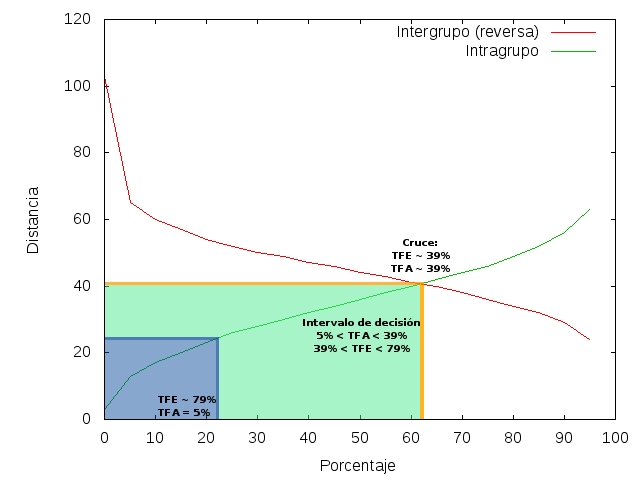
\includegraphics[width=12cm]{imagenes/grafica_TFA.png}
	\caption{Explicación de gráfica TFA/TFE}
	\label{fig:example_TFA}
\end{figure}


\section{Estadísticas}

Las estadísticas a tomar son las siguientes:

\subsection{Estadísticas en localización facial}
El algoritmo empleado es eficiente y eficaz. Hubo 5 falsos negativos sobre 451 imágenes. Sobre las 446 restantes, se hallaron 69 falsos positivos. 

\subsection{Estadísticas de funcionamiento}

\begin{figure}[h!]
	\centering
			\resizebox{7.25cm}{!}{% GNUPLOT: LaTeX picture
\setlength{\unitlength}{0.240900pt}
\ifx\plotpoint\undefined\newsavebox{\plotpoint}\fi
\sbox{\plotpoint}{\rule[-0.200pt]{0.400pt}{0.400pt}}%
\begin{picture}(1500,900)(0,0)
\sbox{\plotpoint}{\rule[-0.200pt]{0.400pt}{0.400pt}}%
\put(211.0,131.0){\rule[-0.200pt]{4.818pt}{0.400pt}}
\put(191,131){\makebox(0,0)[r]{ 0}}
\put(1430.0,131.0){\rule[-0.200pt]{4.818pt}{0.400pt}}
\put(211.0,212.0){\rule[-0.200pt]{4.818pt}{0.400pt}}
\put(191,212){\makebox(0,0)[r]{ 0.1}}
\put(1430.0,212.0){\rule[-0.200pt]{4.818pt}{0.400pt}}
\put(211.0,293.0){\rule[-0.200pt]{4.818pt}{0.400pt}}
\put(191,293){\makebox(0,0)[r]{ 0.2}}
\put(1430.0,293.0){\rule[-0.200pt]{4.818pt}{0.400pt}}
\put(211.0,374.0){\rule[-0.200pt]{4.818pt}{0.400pt}}
\put(191,374){\makebox(0,0)[r]{ 0.3}}
\put(1430.0,374.0){\rule[-0.200pt]{4.818pt}{0.400pt}}
\put(211.0,455.0){\rule[-0.200pt]{4.818pt}{0.400pt}}
\put(191,455){\makebox(0,0)[r]{ 0.4}}
\put(1430.0,455.0){\rule[-0.200pt]{4.818pt}{0.400pt}}
\put(211.0,536.0){\rule[-0.200pt]{4.818pt}{0.400pt}}
\put(191,536){\makebox(0,0)[r]{ 0.5}}
\put(1430.0,536.0){\rule[-0.200pt]{4.818pt}{0.400pt}}
\put(211.0,617.0){\rule[-0.200pt]{4.818pt}{0.400pt}}
\put(191,617){\makebox(0,0)[r]{ 0.6}}
\put(1430.0,617.0){\rule[-0.200pt]{4.818pt}{0.400pt}}
\put(211.0,698.0){\rule[-0.200pt]{4.818pt}{0.400pt}}
\put(191,698){\makebox(0,0)[r]{ 0.7}}
\put(1430.0,698.0){\rule[-0.200pt]{4.818pt}{0.400pt}}
\put(211.0,779.0){\rule[-0.200pt]{4.818pt}{0.400pt}}
\put(191,779){\makebox(0,0)[r]{ 0.8}}
\put(1430.0,779.0){\rule[-0.200pt]{4.818pt}{0.400pt}}
\put(211.0,860.0){\rule[-0.200pt]{4.818pt}{0.400pt}}
\put(191,860){\makebox(0,0)[r]{ 0.9}}
\put(1430.0,860.0){\rule[-0.200pt]{4.818pt}{0.400pt}}
\put(211.0,131.0){\rule[-0.200pt]{0.400pt}{4.818pt}}
\put(211,90){\makebox(0,0){ 0}}
\put(211.0,840.0){\rule[-0.200pt]{0.400pt}{4.818pt}}
\put(335.0,131.0){\rule[-0.200pt]{0.400pt}{4.818pt}}
\put(335,90){\makebox(0,0){ 10}}
\put(335.0,840.0){\rule[-0.200pt]{0.400pt}{4.818pt}}
\put(459.0,131.0){\rule[-0.200pt]{0.400pt}{4.818pt}}
\put(459,90){\makebox(0,0){ 20}}
\put(459.0,840.0){\rule[-0.200pt]{0.400pt}{4.818pt}}
\put(583.0,131.0){\rule[-0.200pt]{0.400pt}{4.818pt}}
\put(583,90){\makebox(0,0){ 30}}
\put(583.0,840.0){\rule[-0.200pt]{0.400pt}{4.818pt}}
\put(707.0,131.0){\rule[-0.200pt]{0.400pt}{4.818pt}}
\put(707,90){\makebox(0,0){ 40}}
\put(707.0,840.0){\rule[-0.200pt]{0.400pt}{4.818pt}}
\put(831.0,131.0){\rule[-0.200pt]{0.400pt}{4.818pt}}
\put(831,90){\makebox(0,0){ 50}}
\put(831.0,840.0){\rule[-0.200pt]{0.400pt}{4.818pt}}
\put(954.0,131.0){\rule[-0.200pt]{0.400pt}{4.818pt}}
\put(954,90){\makebox(0,0){ 60}}
\put(954.0,840.0){\rule[-0.200pt]{0.400pt}{4.818pt}}
\put(1078.0,131.0){\rule[-0.200pt]{0.400pt}{4.818pt}}
\put(1078,90){\makebox(0,0){ 70}}
\put(1078.0,840.0){\rule[-0.200pt]{0.400pt}{4.818pt}}
\put(1202.0,131.0){\rule[-0.200pt]{0.400pt}{4.818pt}}
\put(1202,90){\makebox(0,0){ 80}}
\put(1202.0,840.0){\rule[-0.200pt]{0.400pt}{4.818pt}}
\put(1326.0,131.0){\rule[-0.200pt]{0.400pt}{4.818pt}}
\put(1326,90){\makebox(0,0){ 90}}
\put(1326.0,840.0){\rule[-0.200pt]{0.400pt}{4.818pt}}
\put(1450.0,131.0){\rule[-0.200pt]{0.400pt}{4.818pt}}
\put(1450,90){\makebox(0,0){ 100}}
\put(1450.0,840.0){\rule[-0.200pt]{0.400pt}{4.818pt}}
\put(211.0,131.0){\rule[-0.200pt]{0.400pt}{175.616pt}}
\put(211.0,131.0){\rule[-0.200pt]{298.475pt}{0.400pt}}
\put(1450.0,131.0){\rule[-0.200pt]{0.400pt}{175.616pt}}
\put(211.0,860.0){\rule[-0.200pt]{298.475pt}{0.400pt}}
\put(70,495){\makebox(0,0){\rotatebox{90}{\textsf{\small{Distancia}}}}}
\put(830,29){\makebox(0,0){\textsf{\small{Porcentaje}}}}
\sbox{\plotpoint}{\rule[-0.400pt]{0.800pt}{0.800pt}}%
\sbox{\plotpoint}{\rule[-0.200pt]{0.400pt}{0.400pt}}%
\put(1290,820){\makebox(0,0)[r]{\textsf{\small{Intergrupo (reversa)}}}}
\sbox{\plotpoint}{\rule[-0.400pt]{0.800pt}{0.800pt}}%
\put(1310.0,820.0){\rule[-0.400pt]{24.090pt}{0.800pt}}
\put(211,782){\usebox{\plotpoint}}
\multiput(212.41,770.67)(0.502,-1.592){117}{\rule{0.121pt}{2.729pt}}
\multiput(209.34,776.34)(62.000,-190.336){2}{\rule{0.800pt}{1.365pt}}
\multiput(273.00,584.09)(0.543,-0.502){107}{\rule{1.070pt}{0.121pt}}
\multiput(273.00,584.34)(59.779,-57.000){2}{\rule{0.535pt}{0.800pt}}
\multiput(335.00,527.09)(1.315,-0.504){41}{\rule{2.267pt}{0.122pt}}
\multiput(335.00,527.34)(57.295,-24.000){2}{\rule{1.133pt}{0.800pt}}
\multiput(397.00,503.09)(2.013,-0.507){25}{\rule{3.300pt}{0.122pt}}
\multiput(397.00,503.34)(55.151,-16.000){2}{\rule{1.650pt}{0.800pt}}
\multiput(459.00,487.08)(2.751,-0.511){17}{\rule{4.333pt}{0.123pt}}
\multiput(459.00,487.34)(53.006,-12.000){2}{\rule{2.167pt}{0.800pt}}
\multiput(521.00,475.08)(3.382,-0.514){13}{\rule{5.160pt}{0.124pt}}
\multiput(521.00,475.34)(51.290,-10.000){2}{\rule{2.580pt}{0.800pt}}
\multiput(583.00,465.08)(4.429,-0.520){9}{\rule{6.400pt}{0.125pt}}
\multiput(583.00,465.34)(48.716,-8.000){2}{\rule{3.200pt}{0.800pt}}
\multiput(645.00,457.08)(5.293,-0.526){7}{\rule{7.286pt}{0.127pt}}
\multiput(645.00,457.34)(46.878,-7.000){2}{\rule{3.643pt}{0.800pt}}
\multiput(707.00,450.07)(6.714,-0.536){5}{\rule{8.467pt}{0.129pt}}
\multiput(707.00,450.34)(44.427,-6.000){2}{\rule{4.233pt}{0.800pt}}
\multiput(769.00,444.08)(5.293,-0.526){7}{\rule{7.286pt}{0.127pt}}
\multiput(769.00,444.34)(46.878,-7.000){2}{\rule{3.643pt}{0.800pt}}
\multiput(831.00,437.06)(9.828,-0.560){3}{\rule{9.960pt}{0.135pt}}
\multiput(831.00,437.34)(40.328,-5.000){2}{\rule{4.980pt}{0.800pt}}
\multiput(892.00,432.07)(6.714,-0.536){5}{\rule{8.467pt}{0.129pt}}
\multiput(892.00,432.34)(44.427,-6.000){2}{\rule{4.233pt}{0.800pt}}
\multiput(954.00,426.07)(6.714,-0.536){5}{\rule{8.467pt}{0.129pt}}
\multiput(954.00,426.34)(44.427,-6.000){2}{\rule{4.233pt}{0.800pt}}
\multiput(1016.00,420.07)(6.714,-0.536){5}{\rule{8.467pt}{0.129pt}}
\multiput(1016.00,420.34)(44.427,-6.000){2}{\rule{4.233pt}{0.800pt}}
\multiput(1078.00,414.07)(6.714,-0.536){5}{\rule{8.467pt}{0.129pt}}
\multiput(1078.00,414.34)(44.427,-6.000){2}{\rule{4.233pt}{0.800pt}}
\multiput(1140.00,408.07)(6.714,-0.536){5}{\rule{8.467pt}{0.129pt}}
\multiput(1140.00,408.34)(44.427,-6.000){2}{\rule{4.233pt}{0.800pt}}
\multiput(1202.00,402.08)(4.429,-0.520){9}{\rule{6.400pt}{0.125pt}}
\multiput(1202.00,402.34)(48.716,-8.000){2}{\rule{3.200pt}{0.800pt}}
\multiput(1264.00,394.08)(3.829,-0.516){11}{\rule{5.711pt}{0.124pt}}
\multiput(1264.00,394.34)(50.146,-9.000){2}{\rule{2.856pt}{0.800pt}}
\multiput(1326.00,385.08)(2.751,-0.511){17}{\rule{4.333pt}{0.123pt}}
\multiput(1326.00,385.34)(53.006,-12.000){2}{\rule{2.167pt}{0.800pt}}
\sbox{\plotpoint}{\rule[-0.600pt]{1.200pt}{1.200pt}}%
\sbox{\plotpoint}{\rule[-0.200pt]{0.400pt}{0.400pt}}%
\put(1290,779){\makebox(0,0)[r]{\textsf{\small{Intragrupo}}}}
\sbox{\plotpoint}{\rule[-0.600pt]{1.200pt}{1.200pt}}%
\put(1310.0,779.0){\rule[-0.600pt]{24.090pt}{1.200pt}}
\put(211,203){\usebox{\plotpoint}}
\multiput(213.24,203.00)(0.500,0.648){114}{\rule{0.120pt}{1.868pt}}
\multiput(208.51,203.00)(62.000,77.123){2}{\rule{1.200pt}{0.934pt}}
\multiput(273.00,286.24)(1.744,0.501){26}{\rule{4.433pt}{0.121pt}}
\multiput(273.00,281.51)(52.798,18.000){2}{\rule{2.217pt}{1.200pt}}
\multiput(335.00,304.24)(2.694,0.501){14}{\rule{6.500pt}{0.121pt}}
\multiput(335.00,299.51)(48.509,12.000){2}{\rule{3.250pt}{1.200pt}}
\multiput(397.00,316.24)(3.319,0.502){10}{\rule{7.740pt}{0.121pt}}
\multiput(397.00,311.51)(45.935,10.000){2}{\rule{3.870pt}{1.200pt}}
\multiput(459.00,326.24)(4.430,0.503){6}{\rule{9.600pt}{0.121pt}}
\multiput(459.00,321.51)(42.075,8.000){2}{\rule{4.800pt}{1.200pt}}
\multiput(521.00,334.24)(3.777,0.502){8}{\rule{8.567pt}{0.121pt}}
\multiput(521.00,329.51)(44.219,9.000){2}{\rule{4.283pt}{1.200pt}}
\multiput(583.00,343.24)(5.545,0.505){4}{\rule{10.929pt}{0.122pt}}
\multiput(583.00,338.51)(39.317,7.000){2}{\rule{5.464pt}{1.200pt}}
\multiput(645.00,350.24)(4.430,0.503){6}{\rule{9.600pt}{0.121pt}}
\multiput(645.00,345.51)(42.075,8.000){2}{\rule{4.800pt}{1.200pt}}
\multiput(707.00,358.24)(5.545,0.505){4}{\rule{10.929pt}{0.122pt}}
\multiput(707.00,353.51)(39.317,7.000){2}{\rule{5.464pt}{1.200pt}}
\multiput(769.00,365.24)(4.430,0.503){6}{\rule{9.600pt}{0.121pt}}
\multiput(769.00,360.51)(42.075,8.000){2}{\rule{4.800pt}{1.200pt}}
\multiput(831.00,373.24)(4.354,0.503){6}{\rule{9.450pt}{0.121pt}}
\multiput(831.00,368.51)(41.386,8.000){2}{\rule{4.725pt}{1.200pt}}
\multiput(892.00,381.24)(5.545,0.505){4}{\rule{10.929pt}{0.122pt}}
\multiput(892.00,376.51)(39.317,7.000){2}{\rule{5.464pt}{1.200pt}}
\multiput(954.00,388.24)(4.430,0.503){6}{\rule{9.600pt}{0.121pt}}
\multiput(954.00,383.51)(42.075,8.000){2}{\rule{4.800pt}{1.200pt}}
\multiput(1016.00,396.24)(3.319,0.502){10}{\rule{7.740pt}{0.121pt}}
\multiput(1016.00,391.51)(45.935,10.000){2}{\rule{3.870pt}{1.200pt}}
\multiput(1078.00,406.24)(2.694,0.501){14}{\rule{6.500pt}{0.121pt}}
\multiput(1078.00,401.51)(48.509,12.000){2}{\rule{3.250pt}{1.200pt}}
\multiput(1140.00,418.24)(2.114,0.501){20}{\rule{5.260pt}{0.121pt}}
\multiput(1140.00,413.51)(51.083,15.000){2}{\rule{2.630pt}{1.200pt}}
\multiput(1202.00,433.24)(1.352,0.501){36}{\rule{3.535pt}{0.121pt}}
\multiput(1202.00,428.51)(54.663,23.000){2}{\rule{1.767pt}{1.200pt}}
\multiput(1264.00,456.24)(1.066,0.500){48}{\rule{2.866pt}{0.121pt}}
\multiput(1264.00,451.51)(56.052,29.000){2}{\rule{1.433pt}{1.200pt}}
\multiput(1328.24,483.00)(0.500,0.551){114}{\rule{0.120pt}{1.635pt}}
\multiput(1323.51,483.00)(62.000,65.605){2}{\rule{1.200pt}{0.818pt}}
\sbox{\plotpoint}{\rule[-0.200pt]{0.400pt}{0.400pt}}%
\put(211.0,131.0){\rule[-0.200pt]{0.400pt}{175.616pt}}
\put(211.0,131.0){\rule[-0.200pt]{298.475pt}{0.400pt}}
\put(1450.0,131.0){\rule[-0.200pt]{0.400pt}{175.616pt}}
\put(211.0,860.0){\rule[-0.200pt]{298.475pt}{0.400pt}}
\end{picture}
}
			\resizebox{7.25cm}{!}{% GNUPLOT: LaTeX picture
\setlength{\unitlength}{0.240900pt}
\ifx\plotpoint\undefined\newsavebox{\plotpoint}\fi
\begin{picture}(1500,900)(0,0)
\sbox{\plotpoint}{\rule[-0.200pt]{0.400pt}{0.400pt}}%
\put(211.0,131.0){\rule[-0.200pt]{4.818pt}{0.400pt}}
\put(191,131){\makebox(0,0)[r]{ 0}}
\put(1430.0,131.0){\rule[-0.200pt]{4.818pt}{0.400pt}}
\put(211.0,212.0){\rule[-0.200pt]{4.818pt}{0.400pt}}
\put(191,212){\makebox(0,0)[r]{ 0.1}}
\put(1430.0,212.0){\rule[-0.200pt]{4.818pt}{0.400pt}}
\put(211.0,293.0){\rule[-0.200pt]{4.818pt}{0.400pt}}
\put(191,293){\makebox(0,0)[r]{ 0.2}}
\put(1430.0,293.0){\rule[-0.200pt]{4.818pt}{0.400pt}}
\put(211.0,374.0){\rule[-0.200pt]{4.818pt}{0.400pt}}
\put(191,374){\makebox(0,0)[r]{ 0.3}}
\put(1430.0,374.0){\rule[-0.200pt]{4.818pt}{0.400pt}}
\put(211.0,455.0){\rule[-0.200pt]{4.818pt}{0.400pt}}
\put(191,455){\makebox(0,0)[r]{ 0.4}}
\put(1430.0,455.0){\rule[-0.200pt]{4.818pt}{0.400pt}}
\put(211.0,536.0){\rule[-0.200pt]{4.818pt}{0.400pt}}
\put(191,536){\makebox(0,0)[r]{ 0.5}}
\put(1430.0,536.0){\rule[-0.200pt]{4.818pt}{0.400pt}}
\put(211.0,617.0){\rule[-0.200pt]{4.818pt}{0.400pt}}
\put(191,617){\makebox(0,0)[r]{ 0.6}}
\put(1430.0,617.0){\rule[-0.200pt]{4.818pt}{0.400pt}}
\put(211.0,698.0){\rule[-0.200pt]{4.818pt}{0.400pt}}
\put(191,698){\makebox(0,0)[r]{ 0.7}}
\put(1430.0,698.0){\rule[-0.200pt]{4.818pt}{0.400pt}}
\put(211.0,779.0){\rule[-0.200pt]{4.818pt}{0.400pt}}
\put(191,779){\makebox(0,0)[r]{ 0.8}}
\put(1430.0,779.0){\rule[-0.200pt]{4.818pt}{0.400pt}}
\put(211.0,860.0){\rule[-0.200pt]{4.818pt}{0.400pt}}
\put(191,860){\makebox(0,0)[r]{ 0.9}}
\put(1430.0,860.0){\rule[-0.200pt]{4.818pt}{0.400pt}}
\put(211.0,131.0){\rule[-0.200pt]{0.400pt}{4.818pt}}
\put(211,90){\makebox(0,0){ 0}}
\put(211.0,840.0){\rule[-0.200pt]{0.400pt}{4.818pt}}
\put(335.0,131.0){\rule[-0.200pt]{0.400pt}{4.818pt}}
\put(335,90){\makebox(0,0){ 10}}
\put(335.0,840.0){\rule[-0.200pt]{0.400pt}{4.818pt}}
\put(459.0,131.0){\rule[-0.200pt]{0.400pt}{4.818pt}}
\put(459,90){\makebox(0,0){ 20}}
\put(459.0,840.0){\rule[-0.200pt]{0.400pt}{4.818pt}}
\put(583.0,131.0){\rule[-0.200pt]{0.400pt}{4.818pt}}
\put(583,90){\makebox(0,0){ 30}}
\put(583.0,840.0){\rule[-0.200pt]{0.400pt}{4.818pt}}
\put(707.0,131.0){\rule[-0.200pt]{0.400pt}{4.818pt}}
\put(707,90){\makebox(0,0){ 40}}
\put(707.0,840.0){\rule[-0.200pt]{0.400pt}{4.818pt}}
\put(831.0,131.0){\rule[-0.200pt]{0.400pt}{4.818pt}}
\put(831,90){\makebox(0,0){ 50}}
\put(831.0,840.0){\rule[-0.200pt]{0.400pt}{4.818pt}}
\put(954.0,131.0){\rule[-0.200pt]{0.400pt}{4.818pt}}
\put(954,90){\makebox(0,0){ 60}}
\put(954.0,840.0){\rule[-0.200pt]{0.400pt}{4.818pt}}
\put(1078.0,131.0){\rule[-0.200pt]{0.400pt}{4.818pt}}
\put(1078,90){\makebox(0,0){ 70}}
\put(1078.0,840.0){\rule[-0.200pt]{0.400pt}{4.818pt}}
\put(1202.0,131.0){\rule[-0.200pt]{0.400pt}{4.818pt}}
\put(1202,90){\makebox(0,0){ 80}}
\put(1202.0,840.0){\rule[-0.200pt]{0.400pt}{4.818pt}}
\put(1326.0,131.0){\rule[-0.200pt]{0.400pt}{4.818pt}}
\put(1326,90){\makebox(0,0){ 90}}
\put(1326.0,840.0){\rule[-0.200pt]{0.400pt}{4.818pt}}
\put(1450.0,131.0){\rule[-0.200pt]{0.400pt}{4.818pt}}
\put(1450,90){\makebox(0,0){ 100}}
\put(1450.0,840.0){\rule[-0.200pt]{0.400pt}{4.818pt}}
\put(211.0,131.0){\rule[-0.200pt]{0.400pt}{175.616pt}}
\put(211.0,131.0){\rule[-0.200pt]{298.475pt}{0.400pt}}
\put(1450.0,131.0){\rule[-0.200pt]{0.400pt}{175.616pt}}
\put(211.0,860.0){\rule[-0.200pt]{298.475pt}{0.400pt}}
\put(70,495){\makebox(0,0){\rotatebox{90}{\textsf{\small{Distancia}}}}}
\put(830,29){\makebox(0,0){\textsf{\small{Porcentaje}}}}
\sbox{\plotpoint}{\rule[-0.400pt]{0.800pt}{0.800pt}}%
\sbox{\plotpoint}{\rule[-0.200pt]{0.400pt}{0.400pt}}%
\put(1290,820){\makebox(0,0)[r]{\textsf{\small{Intergrupo (reversa)}}}}
\sbox{\plotpoint}{\rule[-0.400pt]{0.800pt}{0.800pt}}%
\put(1310.0,820.0){\rule[-0.400pt]{24.090pt}{0.800pt}}
\put(211,856){\usebox{\plotpoint}}
\multiput(212.41,843.23)(0.502,-1.812){117}{\rule{0.121pt}{3.077pt}}
\multiput(209.34,849.61)(62.000,-216.613){2}{\rule{0.800pt}{1.539pt}}
\multiput(273.00,631.09)(1.210,-0.504){45}{\rule{2.108pt}{0.121pt}}
\multiput(273.00,631.34)(57.625,-26.000){2}{\rule{1.054pt}{0.800pt}}
\multiput(335.00,605.09)(1.887,-0.507){27}{\rule{3.118pt}{0.122pt}}
\multiput(335.00,605.34)(55.529,-17.000){2}{\rule{1.559pt}{0.800pt}}
\multiput(397.00,588.08)(2.518,-0.509){19}{\rule{4.015pt}{0.123pt}}
\multiput(397.00,588.34)(53.666,-13.000){2}{\rule{2.008pt}{0.800pt}}
\multiput(459.00,575.08)(3.032,-0.512){15}{\rule{4.709pt}{0.123pt}}
\multiput(459.00,575.34)(52.226,-11.000){2}{\rule{2.355pt}{0.800pt}}
\multiput(521.00,564.08)(3.829,-0.516){11}{\rule{5.711pt}{0.124pt}}
\multiput(521.00,564.34)(50.146,-9.000){2}{\rule{2.856pt}{0.800pt}}
\multiput(583.00,555.08)(3.829,-0.516){11}{\rule{5.711pt}{0.124pt}}
\multiput(583.00,555.34)(50.146,-9.000){2}{\rule{2.856pt}{0.800pt}}
\multiput(645.00,546.08)(4.429,-0.520){9}{\rule{6.400pt}{0.125pt}}
\multiput(645.00,546.34)(48.716,-8.000){2}{\rule{3.200pt}{0.800pt}}
\multiput(707.00,538.08)(3.829,-0.516){11}{\rule{5.711pt}{0.124pt}}
\multiput(707.00,538.34)(50.146,-9.000){2}{\rule{2.856pt}{0.800pt}}
\multiput(769.00,529.08)(5.293,-0.526){7}{\rule{7.286pt}{0.127pt}}
\multiput(769.00,529.34)(46.878,-7.000){2}{\rule{3.643pt}{0.800pt}}
\multiput(831.00,522.08)(4.356,-0.520){9}{\rule{6.300pt}{0.125pt}}
\multiput(831.00,522.34)(47.924,-8.000){2}{\rule{3.150pt}{0.800pt}}
\multiput(892.00,514.08)(4.429,-0.520){9}{\rule{6.400pt}{0.125pt}}
\multiput(892.00,514.34)(48.716,-8.000){2}{\rule{3.200pt}{0.800pt}}
\multiput(954.00,506.08)(4.429,-0.520){9}{\rule{6.400pt}{0.125pt}}
\multiput(954.00,506.34)(48.716,-8.000){2}{\rule{3.200pt}{0.800pt}}
\multiput(1016.00,498.08)(3.829,-0.516){11}{\rule{5.711pt}{0.124pt}}
\multiput(1016.00,498.34)(50.146,-9.000){2}{\rule{2.856pt}{0.800pt}}
\multiput(1078.00,489.08)(3.829,-0.516){11}{\rule{5.711pt}{0.124pt}}
\multiput(1078.00,489.34)(50.146,-9.000){2}{\rule{2.856pt}{0.800pt}}
\multiput(1140.00,480.08)(3.032,-0.512){15}{\rule{4.709pt}{0.123pt}}
\multiput(1140.00,480.34)(52.226,-11.000){2}{\rule{2.355pt}{0.800pt}}
\multiput(1202.00,469.08)(3.032,-0.512){15}{\rule{4.709pt}{0.123pt}}
\multiput(1202.00,469.34)(52.226,-11.000){2}{\rule{2.355pt}{0.800pt}}
\multiput(1264.00,458.09)(2.323,-0.509){21}{\rule{3.743pt}{0.123pt}}
\multiput(1264.00,458.34)(54.232,-14.000){2}{\rule{1.871pt}{0.800pt}}
\multiput(1326.00,444.09)(1.511,-0.505){35}{\rule{2.562pt}{0.122pt}}
\multiput(1326.00,444.34)(56.683,-21.000){2}{\rule{1.281pt}{0.800pt}}
\sbox{\plotpoint}{\rule[-0.600pt]{1.200pt}{1.200pt}}%
\sbox{\plotpoint}{\rule[-0.200pt]{0.400pt}{0.400pt}}%
\put(1290,779){\makebox(0,0)[r]{\textsf{\small{Intragrupo}}}}
\sbox{\plotpoint}{\rule[-0.600pt]{1.200pt}{1.200pt}}%
\put(1310.0,779.0){\rule[-0.600pt]{24.090pt}{1.200pt}}
\put(211,180){\usebox{\plotpoint}}
\multiput(213.24,180.00)(0.500,0.933){114}{\rule{0.120pt}{2.545pt}}
\multiput(208.51,180.00)(62.000,110.717){2}{\rule{1.200pt}{1.273pt}}
\multiput(273.00,298.24)(1.105,0.500){46}{\rule{2.957pt}{0.121pt}}
\multiput(273.00,293.51)(55.862,28.000){2}{\rule{1.479pt}{1.200pt}}
\multiput(335.00,326.24)(1.974,0.501){22}{\rule{4.950pt}{0.121pt}}
\multiput(335.00,321.51)(51.726,16.000){2}{\rule{2.475pt}{1.200pt}}
\multiput(397.00,342.24)(2.114,0.501){20}{\rule{5.260pt}{0.121pt}}
\multiput(397.00,337.51)(51.083,15.000){2}{\rule{2.630pt}{1.200pt}}
\multiput(459.00,357.24)(2.467,0.501){16}{\rule{6.023pt}{0.121pt}}
\multiput(459.00,352.51)(49.499,13.000){2}{\rule{3.012pt}{1.200pt}}
\multiput(521.00,370.24)(2.276,0.501){18}{\rule{5.614pt}{0.121pt}}
\multiput(521.00,365.51)(50.347,14.000){2}{\rule{2.807pt}{1.200pt}}
\multiput(583.00,384.24)(2.971,0.502){12}{\rule{7.064pt}{0.121pt}}
\multiput(583.00,379.51)(47.339,11.000){2}{\rule{3.532pt}{1.200pt}}
\multiput(645.00,395.24)(2.276,0.501){18}{\rule{5.614pt}{0.121pt}}
\multiput(645.00,390.51)(50.347,14.000){2}{\rule{2.807pt}{1.200pt}}
\multiput(707.00,409.24)(2.694,0.501){14}{\rule{6.500pt}{0.121pt}}
\multiput(707.00,404.51)(48.509,12.000){2}{\rule{3.250pt}{1.200pt}}
\multiput(769.00,421.24)(2.694,0.501){14}{\rule{6.500pt}{0.121pt}}
\multiput(769.00,416.51)(48.509,12.000){2}{\rule{3.250pt}{1.200pt}}
\multiput(831.00,433.24)(2.921,0.502){12}{\rule{6.955pt}{0.121pt}}
\multiput(831.00,428.51)(46.565,11.000){2}{\rule{3.477pt}{1.200pt}}
\multiput(892.00,444.24)(2.467,0.501){16}{\rule{6.023pt}{0.121pt}}
\multiput(892.00,439.51)(49.499,13.000){2}{\rule{3.012pt}{1.200pt}}
\multiput(954.00,457.24)(2.276,0.501){18}{\rule{5.614pt}{0.121pt}}
\multiput(954.00,452.51)(50.347,14.000){2}{\rule{2.807pt}{1.200pt}}
\multiput(1016.00,471.24)(2.114,0.501){20}{\rule{5.260pt}{0.121pt}}
\multiput(1016.00,466.51)(51.083,15.000){2}{\rule{2.630pt}{1.200pt}}
\multiput(1078.00,486.24)(2.114,0.501){20}{\rule{5.260pt}{0.121pt}}
\multiput(1078.00,481.51)(51.083,15.000){2}{\rule{2.630pt}{1.200pt}}
\multiput(1140.00,501.24)(1.744,0.501){26}{\rule{4.433pt}{0.121pt}}
\multiput(1140.00,496.51)(52.798,18.000){2}{\rule{2.217pt}{1.200pt}}
\multiput(1202.00,519.24)(1.563,0.501){30}{\rule{4.020pt}{0.121pt}}
\multiput(1202.00,514.51)(53.656,20.000){2}{\rule{2.010pt}{1.200pt}}
\multiput(1264.00,539.24)(1.105,0.500){46}{\rule{2.957pt}{0.121pt}}
\multiput(1264.00,534.51)(55.862,28.000){2}{\rule{1.479pt}{1.200pt}}
\multiput(1326.00,567.24)(0.698,0.500){78}{\rule{1.991pt}{0.121pt}}
\multiput(1326.00,562.51)(57.868,44.000){2}{\rule{0.995pt}{1.200pt}}
\sbox{\plotpoint}{\rule[-0.200pt]{0.400pt}{0.400pt}}%
\put(211.0,131.0){\rule[-0.200pt]{0.400pt}{175.616pt}}
\put(211.0,131.0){\rule[-0.200pt]{298.475pt}{0.400pt}}
\put(1450.0,131.0){\rule[-0.200pt]{0.400pt}{175.616pt}}
\put(211.0,860.0){\rule[-0.200pt]{298.475pt}{0.400pt}}
\end{picture}
}
			\resizebox{7.25cm}{!}{% GNUPLOT: LaTeX picture
\setlength{\unitlength}{0.240900pt}
\ifx\plotpoint\undefined\newsavebox{\plotpoint}\fi
\begin{picture}(1500,900)(0,0)
\sbox{\plotpoint}{\rule[-0.200pt]{0.400pt}{0.400pt}}%
\put(211.0,131.0){\rule[-0.200pt]{4.818pt}{0.400pt}}
\put(191,131){\makebox(0,0)[r]{ 0}}
\put(1430.0,131.0){\rule[-0.200pt]{4.818pt}{0.400pt}}
\put(211.0,212.0){\rule[-0.200pt]{4.818pt}{0.400pt}}
\put(191,212){\makebox(0,0)[r]{ 20}}
\put(1430.0,212.0){\rule[-0.200pt]{4.818pt}{0.400pt}}
\put(211.0,293.0){\rule[-0.200pt]{4.818pt}{0.400pt}}
\put(191,293){\makebox(0,0)[r]{ 40}}
\put(1430.0,293.0){\rule[-0.200pt]{4.818pt}{0.400pt}}
\put(211.0,374.0){\rule[-0.200pt]{4.818pt}{0.400pt}}
\put(191,374){\makebox(0,0)[r]{ 60}}
\put(1430.0,374.0){\rule[-0.200pt]{4.818pt}{0.400pt}}
\put(211.0,455.0){\rule[-0.200pt]{4.818pt}{0.400pt}}
\put(191,455){\makebox(0,0)[r]{ 80}}
\put(1430.0,455.0){\rule[-0.200pt]{4.818pt}{0.400pt}}
\put(211.0,536.0){\rule[-0.200pt]{4.818pt}{0.400pt}}
\put(191,536){\makebox(0,0)[r]{ 100}}
\put(1430.0,536.0){\rule[-0.200pt]{4.818pt}{0.400pt}}
\put(211.0,617.0){\rule[-0.200pt]{4.818pt}{0.400pt}}
\put(191,617){\makebox(0,0)[r]{ 120}}
\put(1430.0,617.0){\rule[-0.200pt]{4.818pt}{0.400pt}}
\put(211.0,698.0){\rule[-0.200pt]{4.818pt}{0.400pt}}
\put(191,698){\makebox(0,0)[r]{ 140}}
\put(1430.0,698.0){\rule[-0.200pt]{4.818pt}{0.400pt}}
\put(211.0,779.0){\rule[-0.200pt]{4.818pt}{0.400pt}}
\put(191,779){\makebox(0,0)[r]{ 160}}
\put(1430.0,779.0){\rule[-0.200pt]{4.818pt}{0.400pt}}
\put(211.0,860.0){\rule[-0.200pt]{4.818pt}{0.400pt}}
\put(191,860){\makebox(0,0)[r]{ 180}}
\put(1430.0,860.0){\rule[-0.200pt]{4.818pt}{0.400pt}}
\put(211.0,131.0){\rule[-0.200pt]{0.400pt}{4.818pt}}
\put(211,90){\makebox(0,0){ 0}}
\put(211.0,840.0){\rule[-0.200pt]{0.400pt}{4.818pt}}
\put(335.0,131.0){\rule[-0.200pt]{0.400pt}{4.818pt}}
\put(335,90){\makebox(0,0){ 10}}
\put(335.0,840.0){\rule[-0.200pt]{0.400pt}{4.818pt}}
\put(459.0,131.0){\rule[-0.200pt]{0.400pt}{4.818pt}}
\put(459,90){\makebox(0,0){ 20}}
\put(459.0,840.0){\rule[-0.200pt]{0.400pt}{4.818pt}}
\put(583.0,131.0){\rule[-0.200pt]{0.400pt}{4.818pt}}
\put(583,90){\makebox(0,0){ 30}}
\put(583.0,840.0){\rule[-0.200pt]{0.400pt}{4.818pt}}
\put(707.0,131.0){\rule[-0.200pt]{0.400pt}{4.818pt}}
\put(707,90){\makebox(0,0){ 40}}
\put(707.0,840.0){\rule[-0.200pt]{0.400pt}{4.818pt}}
\put(831.0,131.0){\rule[-0.200pt]{0.400pt}{4.818pt}}
\put(831,90){\makebox(0,0){ 50}}
\put(831.0,840.0){\rule[-0.200pt]{0.400pt}{4.818pt}}
\put(954.0,131.0){\rule[-0.200pt]{0.400pt}{4.818pt}}
\put(954,90){\makebox(0,0){ 60}}
\put(954.0,840.0){\rule[-0.200pt]{0.400pt}{4.818pt}}
\put(1078.0,131.0){\rule[-0.200pt]{0.400pt}{4.818pt}}
\put(1078,90){\makebox(0,0){ 70}}
\put(1078.0,840.0){\rule[-0.200pt]{0.400pt}{4.818pt}}
\put(1202.0,131.0){\rule[-0.200pt]{0.400pt}{4.818pt}}
\put(1202,90){\makebox(0,0){ 80}}
\put(1202.0,840.0){\rule[-0.200pt]{0.400pt}{4.818pt}}
\put(1326.0,131.0){\rule[-0.200pt]{0.400pt}{4.818pt}}
\put(1326,90){\makebox(0,0){ 90}}
\put(1326.0,840.0){\rule[-0.200pt]{0.400pt}{4.818pt}}
\put(1450.0,131.0){\rule[-0.200pt]{0.400pt}{4.818pt}}
\put(1450,90){\makebox(0,0){ 100}}
\put(1450.0,840.0){\rule[-0.200pt]{0.400pt}{4.818pt}}
\put(211.0,131.0){\rule[-0.200pt]{0.400pt}{175.616pt}}
\put(211.0,131.0){\rule[-0.200pt]{298.475pt}{0.400pt}}
\put(1450.0,131.0){\rule[-0.200pt]{0.400pt}{175.616pt}}
\put(211.0,860.0){\rule[-0.200pt]{298.475pt}{0.400pt}}
\put(70,495){\makebox(0,0){\rotatebox{90}{\textsf{\small{Distancia}}}}}
\put(830,29){\makebox(0,0){\textsf{\small{Porcentaje}}}}
\sbox{\plotpoint}{\rule[-0.400pt]{0.800pt}{0.800pt}}%
\sbox{\plotpoint}{\rule[-0.200pt]{0.400pt}{0.400pt}}%
\put(1290,820){\makebox(0,0)[r]{\textsf{\small{Intergrupo (reversa)}}}}
\sbox{\plotpoint}{\rule[-0.400pt]{0.800pt}{0.800pt}}%
\put(1310.0,820.0){\rule[-0.400pt]{24.090pt}{0.800pt}}
\put(211,840){\usebox{\plotpoint}}
\multiput(212.41,830.06)(0.502,-1.380){117}{\rule{0.121pt}{2.394pt}}
\multiput(209.34,835.03)(62.000,-165.032){2}{\rule{0.800pt}{1.197pt}}
\multiput(273.00,668.09)(1.081,-0.504){51}{\rule{1.910pt}{0.121pt}}
\multiput(273.00,668.34)(58.035,-29.000){2}{\rule{0.955pt}{0.800pt}}
\multiput(335.00,639.09)(1.315,-0.504){41}{\rule{2.267pt}{0.122pt}}
\multiput(335.00,639.34)(57.295,-24.000){2}{\rule{1.133pt}{0.800pt}}
\multiput(397.00,615.09)(1.590,-0.505){33}{\rule{2.680pt}{0.122pt}}
\multiput(397.00,615.34)(56.438,-20.000){2}{\rule{1.340pt}{0.800pt}}
\multiput(459.00,595.08)(2.751,-0.511){17}{\rule{4.333pt}{0.123pt}}
\multiput(459.00,595.34)(53.006,-12.000){2}{\rule{2.167pt}{0.800pt}}
\multiput(521.00,583.08)(2.518,-0.509){19}{\rule{4.015pt}{0.123pt}}
\multiput(521.00,583.34)(53.666,-13.000){2}{\rule{2.008pt}{0.800pt}}
\multiput(583.00,570.08)(2.751,-0.511){17}{\rule{4.333pt}{0.123pt}}
\multiput(583.00,570.34)(53.006,-12.000){2}{\rule{2.167pt}{0.800pt}}
\multiput(645.00,558.08)(2.751,-0.511){17}{\rule{4.333pt}{0.123pt}}
\multiput(645.00,558.34)(53.006,-12.000){2}{\rule{2.167pt}{0.800pt}}
\multiput(707.00,546.08)(4.429,-0.520){9}{\rule{6.400pt}{0.125pt}}
\multiput(707.00,546.34)(48.716,-8.000){2}{\rule{3.200pt}{0.800pt}}
\multiput(769.00,538.08)(2.751,-0.511){17}{\rule{4.333pt}{0.123pt}}
\multiput(769.00,538.34)(53.006,-12.000){2}{\rule{2.167pt}{0.800pt}}
\multiput(831.00,526.08)(4.356,-0.520){9}{\rule{6.300pt}{0.125pt}}
\multiput(831.00,526.34)(47.924,-8.000){2}{\rule{3.150pt}{0.800pt}}
\multiput(892.00,518.08)(2.751,-0.511){17}{\rule{4.333pt}{0.123pt}}
\multiput(892.00,518.34)(53.006,-12.000){2}{\rule{2.167pt}{0.800pt}}
\multiput(954.00,506.08)(4.429,-0.520){9}{\rule{6.400pt}{0.125pt}}
\multiput(954.00,506.34)(48.716,-8.000){2}{\rule{3.200pt}{0.800pt}}
\multiput(1016.00,498.08)(2.518,-0.509){19}{\rule{4.015pt}{0.123pt}}
\multiput(1016.00,498.34)(53.666,-13.000){2}{\rule{2.008pt}{0.800pt}}
\multiput(1078.00,485.08)(2.751,-0.511){17}{\rule{4.333pt}{0.123pt}}
\multiput(1078.00,485.34)(53.006,-12.000){2}{\rule{2.167pt}{0.800pt}}
\multiput(1140.00,473.08)(2.751,-0.511){17}{\rule{4.333pt}{0.123pt}}
\multiput(1140.00,473.34)(53.006,-12.000){2}{\rule{2.167pt}{0.800pt}}
\multiput(1202.00,461.08)(2.751,-0.511){17}{\rule{4.333pt}{0.123pt}}
\multiput(1202.00,461.34)(53.006,-12.000){2}{\rule{2.167pt}{0.800pt}}
\multiput(1264.00,449.09)(1.590,-0.505){33}{\rule{2.680pt}{0.122pt}}
\multiput(1264.00,449.34)(56.438,-20.000){2}{\rule{1.340pt}{0.800pt}}
\multiput(1326.00,429.09)(1.260,-0.504){43}{\rule{2.184pt}{0.121pt}}
\multiput(1326.00,429.34)(57.467,-25.000){2}{\rule{1.092pt}{0.800pt}}
\sbox{\plotpoint}{\rule[-0.600pt]{1.200pt}{1.200pt}}%
\sbox{\plotpoint}{\rule[-0.200pt]{0.400pt}{0.400pt}}%
\put(1290,779){\makebox(0,0)[r]{\textsf{\small{Intragrupo}}}}
\sbox{\plotpoint}{\rule[-0.600pt]{1.200pt}{1.200pt}}%
\put(1310.0,779.0){\rule[-0.600pt]{24.090pt}{1.200pt}}
\put(211,200){\usebox{\plotpoint}}
\multiput(213.24,200.00)(0.500,0.551){114}{\rule{0.120pt}{1.635pt}}
\multiput(208.51,200.00)(62.000,65.605){2}{\rule{1.200pt}{0.818pt}}
\multiput(273.00,271.24)(1.563,0.501){30}{\rule{4.020pt}{0.121pt}}
\multiput(273.00,266.51)(53.656,20.000){2}{\rule{2.010pt}{1.200pt}}
\multiput(335.00,291.24)(1.974,0.501){22}{\rule{4.950pt}{0.121pt}}
\multiput(335.00,286.51)(51.726,16.000){2}{\rule{2.475pt}{1.200pt}}
\multiput(397.00,307.24)(1.974,0.501){22}{\rule{4.950pt}{0.121pt}}
\multiput(397.00,302.51)(51.726,16.000){2}{\rule{2.475pt}{1.200pt}}
\multiput(459.00,323.24)(2.467,0.501){16}{\rule{6.023pt}{0.121pt}}
\multiput(459.00,318.51)(49.499,13.000){2}{\rule{3.012pt}{1.200pt}}
\multiput(521.00,336.24)(1.974,0.501){22}{\rule{4.950pt}{0.121pt}}
\multiput(521.00,331.51)(51.726,16.000){2}{\rule{2.475pt}{1.200pt}}
\multiput(583.00,352.24)(2.694,0.501){14}{\rule{6.500pt}{0.121pt}}
\multiput(583.00,347.51)(48.509,12.000){2}{\rule{3.250pt}{1.200pt}}
\multiput(645.00,364.24)(2.694,0.501){14}{\rule{6.500pt}{0.121pt}}
\multiput(645.00,359.51)(48.509,12.000){2}{\rule{3.250pt}{1.200pt}}
\multiput(707.00,376.24)(2.694,0.501){14}{\rule{6.500pt}{0.121pt}}
\multiput(707.00,371.51)(48.509,12.000){2}{\rule{3.250pt}{1.200pt}}
\multiput(769.00,388.24)(1.974,0.501){22}{\rule{4.950pt}{0.121pt}}
\multiput(769.00,383.51)(51.726,16.000){2}{\rule{2.475pt}{1.200pt}}
\multiput(831.00,404.24)(1.821,0.501){24}{\rule{4.606pt}{0.121pt}}
\multiput(831.00,399.51)(51.440,17.000){2}{\rule{2.303pt}{1.200pt}}
\multiput(892.00,421.24)(2.694,0.501){14}{\rule{6.500pt}{0.121pt}}
\multiput(892.00,416.51)(48.509,12.000){2}{\rule{3.250pt}{1.200pt}}
\multiput(954.00,433.24)(1.974,0.501){22}{\rule{4.950pt}{0.121pt}}
\multiput(954.00,428.51)(51.726,16.000){2}{\rule{2.475pt}{1.200pt}}
\multiput(1016.00,449.24)(1.563,0.501){30}{\rule{4.020pt}{0.121pt}}
\multiput(1016.00,444.51)(53.656,20.000){2}{\rule{2.010pt}{1.200pt}}
\multiput(1078.00,469.24)(1.563,0.501){30}{\rule{4.020pt}{0.121pt}}
\multiput(1078.00,464.51)(53.656,20.000){2}{\rule{2.010pt}{1.200pt}}
\multiput(1140.00,489.24)(1.485,0.501){32}{\rule{3.843pt}{0.121pt}}
\multiput(1140.00,484.51)(54.024,21.000){2}{\rule{1.921pt}{1.200pt}}
\multiput(1202.00,510.24)(1.105,0.500){46}{\rule{2.957pt}{0.121pt}}
\multiput(1202.00,505.51)(55.862,28.000){2}{\rule{1.479pt}{1.200pt}}
\multiput(1264.00,538.24)(0.750,0.500){72}{\rule{2.115pt}{0.121pt}}
\multiput(1264.00,533.51)(57.611,41.000){2}{\rule{1.057pt}{1.200pt}}
\multiput(1326.00,579.24)(0.510,0.500){110}{\rule{1.540pt}{0.120pt}}
\multiput(1326.00,574.51)(58.804,60.000){2}{\rule{0.770pt}{1.200pt}}
\sbox{\plotpoint}{\rule[-0.200pt]{0.400pt}{0.400pt}}%
\put(211.0,131.0){\rule[-0.200pt]{0.400pt}{175.616pt}}
\put(211.0,131.0){\rule[-0.200pt]{298.475pt}{0.400pt}}
\put(1450.0,131.0){\rule[-0.200pt]{0.400pt}{175.616pt}}
\put(211.0,860.0){\rule[-0.200pt]{298.475pt}{0.400pt}}
\end{picture}
}
			\resizebox{7.25cm}{!}{% GNUPLOT: LaTeX picture
\setlength{\unitlength}{0.240900pt}
\ifx\plotpoint\undefined\newsavebox{\plotpoint}\fi
\begin{picture}(1500,900)(0,0)
\sbox{\plotpoint}{\rule[-0.200pt]{0.400pt}{0.400pt}}%
\put(211.0,131.0){\rule[-0.200pt]{4.818pt}{0.400pt}}
\put(191,131){\makebox(0,0)[r]{ 0}}
\put(1430.0,131.0){\rule[-0.200pt]{4.818pt}{0.400pt}}
\put(211.0,235.0){\rule[-0.200pt]{4.818pt}{0.400pt}}
\put(191,235){\makebox(0,0)[r]{ 0.1}}
\put(1430.0,235.0){\rule[-0.200pt]{4.818pt}{0.400pt}}
\put(211.0,339.0){\rule[-0.200pt]{4.818pt}{0.400pt}}
\put(191,339){\makebox(0,0)[r]{ 0.2}}
\put(1430.0,339.0){\rule[-0.200pt]{4.818pt}{0.400pt}}
\put(211.0,443.0){\rule[-0.200pt]{4.818pt}{0.400pt}}
\put(191,443){\makebox(0,0)[r]{ 0.3}}
\put(1430.0,443.0){\rule[-0.200pt]{4.818pt}{0.400pt}}
\put(211.0,548.0){\rule[-0.200pt]{4.818pt}{0.400pt}}
\put(191,548){\makebox(0,0)[r]{ 0.4}}
\put(1430.0,548.0){\rule[-0.200pt]{4.818pt}{0.400pt}}
\put(211.0,652.0){\rule[-0.200pt]{4.818pt}{0.400pt}}
\put(191,652){\makebox(0,0)[r]{ 0.5}}
\put(1430.0,652.0){\rule[-0.200pt]{4.818pt}{0.400pt}}
\put(211.0,756.0){\rule[-0.200pt]{4.818pt}{0.400pt}}
\put(191,756){\makebox(0,0)[r]{ 0.6}}
\put(1430.0,756.0){\rule[-0.200pt]{4.818pt}{0.400pt}}
\put(211.0,860.0){\rule[-0.200pt]{4.818pt}{0.400pt}}
\put(191,860){\makebox(0,0)[r]{ 0.7}}
\put(1430.0,860.0){\rule[-0.200pt]{4.818pt}{0.400pt}}
\put(211.0,131.0){\rule[-0.200pt]{0.400pt}{4.818pt}}
\put(211,90){\makebox(0,0){ 0}}
\put(211.0,840.0){\rule[-0.200pt]{0.400pt}{4.818pt}}
\put(335.0,131.0){\rule[-0.200pt]{0.400pt}{4.818pt}}
\put(335,90){\makebox(0,0){ 10}}
\put(335.0,840.0){\rule[-0.200pt]{0.400pt}{4.818pt}}
\put(459.0,131.0){\rule[-0.200pt]{0.400pt}{4.818pt}}
\put(459,90){\makebox(0,0){ 20}}
\put(459.0,840.0){\rule[-0.200pt]{0.400pt}{4.818pt}}
\put(583.0,131.0){\rule[-0.200pt]{0.400pt}{4.818pt}}
\put(583,90){\makebox(0,0){ 30}}
\put(583.0,840.0){\rule[-0.200pt]{0.400pt}{4.818pt}}
\put(707.0,131.0){\rule[-0.200pt]{0.400pt}{4.818pt}}
\put(707,90){\makebox(0,0){ 40}}
\put(707.0,840.0){\rule[-0.200pt]{0.400pt}{4.818pt}}
\put(831.0,131.0){\rule[-0.200pt]{0.400pt}{4.818pt}}
\put(831,90){\makebox(0,0){ 50}}
\put(831.0,840.0){\rule[-0.200pt]{0.400pt}{4.818pt}}
\put(954.0,131.0){\rule[-0.200pt]{0.400pt}{4.818pt}}
\put(954,90){\makebox(0,0){ 60}}
\put(954.0,840.0){\rule[-0.200pt]{0.400pt}{4.818pt}}
\put(1078.0,131.0){\rule[-0.200pt]{0.400pt}{4.818pt}}
\put(1078,90){\makebox(0,0){ 70}}
\put(1078.0,840.0){\rule[-0.200pt]{0.400pt}{4.818pt}}
\put(1202.0,131.0){\rule[-0.200pt]{0.400pt}{4.818pt}}
\put(1202,90){\makebox(0,0){ 80}}
\put(1202.0,840.0){\rule[-0.200pt]{0.400pt}{4.818pt}}
\put(1326.0,131.0){\rule[-0.200pt]{0.400pt}{4.818pt}}
\put(1326,90){\makebox(0,0){ 90}}
\put(1326.0,840.0){\rule[-0.200pt]{0.400pt}{4.818pt}}
\put(1450.0,131.0){\rule[-0.200pt]{0.400pt}{4.818pt}}
\put(1450,90){\makebox(0,0){ 100}}
\put(1450.0,840.0){\rule[-0.200pt]{0.400pt}{4.818pt}}
\put(211.0,131.0){\rule[-0.200pt]{0.400pt}{175.616pt}}
\put(211.0,131.0){\rule[-0.200pt]{298.475pt}{0.400pt}}
\put(1450.0,131.0){\rule[-0.200pt]{0.400pt}{175.616pt}}
\put(211.0,860.0){\rule[-0.200pt]{298.475pt}{0.400pt}}
\put(70,495){\makebox(0,0){\rotatebox{90}{\textsf{\small{Distancia}}}}}
\put(830,29){\makebox(0,0){\textsf{\small{Porcentaje}}}}
\sbox{\plotpoint}{\rule[-0.400pt]{0.800pt}{0.800pt}}%
\sbox{\plotpoint}{\rule[-0.200pt]{0.400pt}{0.400pt}}%
\put(1290,820){\makebox(0,0)[r]{\textsf{\small{Intergrupo (reversa)}}}}
\sbox{\plotpoint}{\rule[-0.400pt]{0.800pt}{0.800pt}}%
\put(1310.0,820.0){\rule[-0.400pt]{24.090pt}{0.800pt}}
\put(211,821){\usebox{\plotpoint}}
\multiput(212.41,805.39)(0.502,-2.245){117}{\rule{0.121pt}{3.761pt}}
\multiput(209.34,813.19)(62.000,-268.193){2}{\rule{0.800pt}{1.881pt}}
\multiput(273.00,543.09)(0.740,-0.502){77}{\rule{1.381pt}{0.121pt}}
\multiput(273.00,543.34)(59.134,-42.000){2}{\rule{0.690pt}{0.800pt}}
\multiput(335.00,501.09)(1.081,-0.504){51}{\rule{1.910pt}{0.121pt}}
\multiput(335.00,501.34)(58.035,-29.000){2}{\rule{0.955pt}{0.800pt}}
\multiput(397.00,472.09)(1.374,-0.505){39}{\rule{2.357pt}{0.122pt}}
\multiput(397.00,472.34)(57.109,-23.000){2}{\rule{1.178pt}{0.800pt}}
\multiput(459.00,449.09)(1.511,-0.505){35}{\rule{2.562pt}{0.122pt}}
\multiput(459.00,449.34)(56.683,-21.000){2}{\rule{1.281pt}{0.800pt}}
\multiput(521.00,428.09)(1.678,-0.506){31}{\rule{2.811pt}{0.122pt}}
\multiput(521.00,428.34)(56.167,-19.000){2}{\rule{1.405pt}{0.800pt}}
\multiput(583.00,409.09)(1.887,-0.507){27}{\rule{3.118pt}{0.122pt}}
\multiput(583.00,409.34)(55.529,-17.000){2}{\rule{1.559pt}{0.800pt}}
\multiput(645.00,392.09)(2.013,-0.507){25}{\rule{3.300pt}{0.122pt}}
\multiput(645.00,392.34)(55.151,-16.000){2}{\rule{1.650pt}{0.800pt}}
\multiput(707.00,376.09)(2.013,-0.507){25}{\rule{3.300pt}{0.122pt}}
\multiput(707.00,376.34)(55.151,-16.000){2}{\rule{1.650pt}{0.800pt}}
\multiput(769.00,360.09)(2.323,-0.509){21}{\rule{3.743pt}{0.123pt}}
\multiput(769.00,360.34)(54.232,-14.000){2}{\rule{1.871pt}{0.800pt}}
\multiput(831.00,346.09)(2.121,-0.508){23}{\rule{3.453pt}{0.122pt}}
\multiput(831.00,346.34)(53.832,-15.000){2}{\rule{1.727pt}{0.800pt}}
\multiput(892.00,331.09)(2.157,-0.508){23}{\rule{3.507pt}{0.122pt}}
\multiput(892.00,331.34)(54.722,-15.000){2}{\rule{1.753pt}{0.800pt}}
\multiput(954.00,316.09)(2.157,-0.508){23}{\rule{3.507pt}{0.122pt}}
\multiput(954.00,316.34)(54.722,-15.000){2}{\rule{1.753pt}{0.800pt}}
\multiput(1016.00,301.09)(2.157,-0.508){23}{\rule{3.507pt}{0.122pt}}
\multiput(1016.00,301.34)(54.722,-15.000){2}{\rule{1.753pt}{0.800pt}}
\multiput(1078.00,286.09)(2.013,-0.507){25}{\rule{3.300pt}{0.122pt}}
\multiput(1078.00,286.34)(55.151,-16.000){2}{\rule{1.650pt}{0.800pt}}
\multiput(1140.00,270.09)(2.013,-0.507){25}{\rule{3.300pt}{0.122pt}}
\multiput(1140.00,270.34)(55.151,-16.000){2}{\rule{1.650pt}{0.800pt}}
\multiput(1202.00,254.09)(1.776,-0.506){29}{\rule{2.956pt}{0.122pt}}
\multiput(1202.00,254.34)(55.866,-18.000){2}{\rule{1.478pt}{0.800pt}}
\multiput(1264.00,236.09)(1.590,-0.505){33}{\rule{2.680pt}{0.122pt}}
\multiput(1264.00,236.34)(56.438,-20.000){2}{\rule{1.340pt}{0.800pt}}
\multiput(1326.00,216.09)(1.164,-0.504){47}{\rule{2.037pt}{0.121pt}}
\multiput(1326.00,216.34)(57.772,-27.000){2}{\rule{1.019pt}{0.800pt}}
\sbox{\plotpoint}{\rule[-0.600pt]{1.200pt}{1.200pt}}%
\sbox{\plotpoint}{\rule[-0.200pt]{0.400pt}{0.400pt}}%
\put(1290,779){\makebox(0,0)[r]{\textsf{\small{Intragrupo}}}}
\sbox{\plotpoint}{\rule[-0.600pt]{1.200pt}{1.200pt}}%
\put(1310.0,779.0){\rule[-0.600pt]{24.090pt}{1.200pt}}
\put(211,131){\usebox{\plotpoint}}
\multiput(213.24,131.00)(0.500,0.819){114}{\rule{0.120pt}{2.274pt}}
\multiput(208.51,131.00)(62.000,97.280){2}{\rule{1.200pt}{1.137pt}}
\multiput(273.00,235.24)(0.613,0.500){90}{\rule{1.788pt}{0.120pt}}
\multiput(273.00,230.51)(58.289,50.000){2}{\rule{0.894pt}{1.200pt}}
\multiput(335.00,285.24)(0.682,0.500){80}{\rule{1.953pt}{0.121pt}}
\multiput(335.00,280.51)(57.946,45.000){2}{\rule{0.977pt}{1.200pt}}
\multiput(397.00,330.24)(0.750,0.500){72}{\rule{2.115pt}{0.121pt}}
\multiput(397.00,325.51)(57.611,41.000){2}{\rule{1.057pt}{1.200pt}}
\multiput(459.00,371.24)(0.832,0.500){64}{\rule{2.311pt}{0.121pt}}
\multiput(459.00,366.51)(57.204,37.000){2}{\rule{1.155pt}{1.200pt}}
\multiput(521.00,408.24)(0.996,0.500){52}{\rule{2.700pt}{0.121pt}}
\multiput(521.00,403.51)(56.396,31.000){2}{\rule{1.350pt}{1.200pt}}
\multiput(583.00,439.24)(1.147,0.500){44}{\rule{3.056pt}{0.121pt}}
\multiput(583.00,434.51)(55.658,27.000){2}{\rule{1.528pt}{1.200pt}}
\multiput(645.00,466.24)(1.192,0.500){42}{\rule{3.162pt}{0.121pt}}
\multiput(645.00,461.51)(55.438,26.000){2}{\rule{1.581pt}{1.200pt}}
\multiput(707.00,492.24)(1.294,0.500){38}{\rule{3.400pt}{0.121pt}}
\multiput(707.00,487.51)(54.943,24.000){2}{\rule{1.700pt}{1.200pt}}
\multiput(769.00,516.24)(1.192,0.500){42}{\rule{3.162pt}{0.121pt}}
\multiput(769.00,511.51)(55.438,26.000){2}{\rule{1.581pt}{1.200pt}}
\multiput(831.00,542.24)(1.461,0.501){32}{\rule{3.786pt}{0.121pt}}
\multiput(831.00,537.51)(53.143,21.000){2}{\rule{1.893pt}{1.200pt}}
\multiput(892.00,563.24)(1.416,0.501){34}{\rule{3.682pt}{0.121pt}}
\multiput(892.00,558.51)(54.358,22.000){2}{\rule{1.841pt}{1.200pt}}
\multiput(954.00,585.24)(1.563,0.501){30}{\rule{4.020pt}{0.121pt}}
\multiput(954.00,580.51)(53.656,20.000){2}{\rule{2.010pt}{1.200pt}}
\multiput(1016.00,605.24)(1.352,0.501){36}{\rule{3.535pt}{0.121pt}}
\multiput(1016.00,600.51)(54.663,23.000){2}{\rule{1.767pt}{1.200pt}}
\multiput(1078.00,628.24)(1.192,0.500){42}{\rule{3.162pt}{0.121pt}}
\multiput(1078.00,623.51)(55.438,26.000){2}{\rule{1.581pt}{1.200pt}}
\multiput(1140.00,654.24)(1.147,0.500){44}{\rule{3.056pt}{0.121pt}}
\multiput(1140.00,649.51)(55.658,27.000){2}{\rule{1.528pt}{1.200pt}}
\multiput(1202.00,681.24)(0.996,0.500){52}{\rule{2.700pt}{0.121pt}}
\multiput(1202.00,676.51)(56.396,31.000){2}{\rule{1.350pt}{1.200pt}}
\multiput(1264.00,712.24)(0.880,0.500){60}{\rule{2.426pt}{0.121pt}}
\multiput(1264.00,707.51)(56.965,35.000){2}{\rule{1.213pt}{1.200pt}}
\multiput(1326.00,747.24)(0.510,0.500){110}{\rule{1.540pt}{0.120pt}}
\multiput(1326.00,742.51)(58.804,60.000){2}{\rule{0.770pt}{1.200pt}}
\sbox{\plotpoint}{\rule[-0.200pt]{0.400pt}{0.400pt}}%
\put(211.0,131.0){\rule[-0.200pt]{0.400pt}{175.616pt}}
\put(211.0,131.0){\rule[-0.200pt]{298.475pt}{0.400pt}}
\put(1450.0,131.0){\rule[-0.200pt]{0.400pt}{175.616pt}}
\put(211.0,860.0){\rule[-0.200pt]{298.475pt}{0.400pt}}
\end{picture}
}
			\resizebox{7.25cm}{!}{% GNUPLOT: LaTeX picture
\setlength{\unitlength}{0.240900pt}
\ifx\plotpoint\undefined\newsavebox{\plotpoint}\fi
\begin{picture}(1500,900)(0,0)
\sbox{\plotpoint}{\rule[-0.200pt]{0.400pt}{0.400pt}}%
\put(211.0,131.0){\rule[-0.200pt]{4.818pt}{0.400pt}}
\put(191,131){\makebox(0,0)[r]{ 0}}
\put(1430.0,131.0){\rule[-0.200pt]{4.818pt}{0.400pt}}
\put(211.0,253.0){\rule[-0.200pt]{4.818pt}{0.400pt}}
\put(191,253){\makebox(0,0)[r]{ 20}}
\put(1430.0,253.0){\rule[-0.200pt]{4.818pt}{0.400pt}}
\put(211.0,374.0){\rule[-0.200pt]{4.818pt}{0.400pt}}
\put(191,374){\makebox(0,0)[r]{ 40}}
\put(1430.0,374.0){\rule[-0.200pt]{4.818pt}{0.400pt}}
\put(211.0,496.0){\rule[-0.200pt]{4.818pt}{0.400pt}}
\put(191,496){\makebox(0,0)[r]{ 60}}
\put(1430.0,496.0){\rule[-0.200pt]{4.818pt}{0.400pt}}
\put(211.0,617.0){\rule[-0.200pt]{4.818pt}{0.400pt}}
\put(191,617){\makebox(0,0)[r]{ 80}}
\put(1430.0,617.0){\rule[-0.200pt]{4.818pt}{0.400pt}}
\put(211.0,739.0){\rule[-0.200pt]{4.818pt}{0.400pt}}
\put(191,739){\makebox(0,0)[r]{ 100}}
\put(1430.0,739.0){\rule[-0.200pt]{4.818pt}{0.400pt}}
\put(211.0,860.0){\rule[-0.200pt]{4.818pt}{0.400pt}}
\put(191,860){\makebox(0,0)[r]{ 120}}
\put(1430.0,860.0){\rule[-0.200pt]{4.818pt}{0.400pt}}
\put(211.0,131.0){\rule[-0.200pt]{0.400pt}{4.818pt}}
\put(211,90){\makebox(0,0){ 0}}
\put(211.0,840.0){\rule[-0.200pt]{0.400pt}{4.818pt}}
\put(335.0,131.0){\rule[-0.200pt]{0.400pt}{4.818pt}}
\put(335,90){\makebox(0,0){ 10}}
\put(335.0,840.0){\rule[-0.200pt]{0.400pt}{4.818pt}}
\put(459.0,131.0){\rule[-0.200pt]{0.400pt}{4.818pt}}
\put(459,90){\makebox(0,0){ 20}}
\put(459.0,840.0){\rule[-0.200pt]{0.400pt}{4.818pt}}
\put(583.0,131.0){\rule[-0.200pt]{0.400pt}{4.818pt}}
\put(583,90){\makebox(0,0){ 30}}
\put(583.0,840.0){\rule[-0.200pt]{0.400pt}{4.818pt}}
\put(707.0,131.0){\rule[-0.200pt]{0.400pt}{4.818pt}}
\put(707,90){\makebox(0,0){ 40}}
\put(707.0,840.0){\rule[-0.200pt]{0.400pt}{4.818pt}}
\put(831.0,131.0){\rule[-0.200pt]{0.400pt}{4.818pt}}
\put(831,90){\makebox(0,0){ 50}}
\put(831.0,840.0){\rule[-0.200pt]{0.400pt}{4.818pt}}
\put(954.0,131.0){\rule[-0.200pt]{0.400pt}{4.818pt}}
\put(954,90){\makebox(0,0){ 60}}
\put(954.0,840.0){\rule[-0.200pt]{0.400pt}{4.818pt}}
\put(1078.0,131.0){\rule[-0.200pt]{0.400pt}{4.818pt}}
\put(1078,90){\makebox(0,0){ 70}}
\put(1078.0,840.0){\rule[-0.200pt]{0.400pt}{4.818pt}}
\put(1202.0,131.0){\rule[-0.200pt]{0.400pt}{4.818pt}}
\put(1202,90){\makebox(0,0){ 80}}
\put(1202.0,840.0){\rule[-0.200pt]{0.400pt}{4.818pt}}
\put(1326.0,131.0){\rule[-0.200pt]{0.400pt}{4.818pt}}
\put(1326,90){\makebox(0,0){ 90}}
\put(1326.0,840.0){\rule[-0.200pt]{0.400pt}{4.818pt}}
\put(1450.0,131.0){\rule[-0.200pt]{0.400pt}{4.818pt}}
\put(1450,90){\makebox(0,0){ 100}}
\put(1450.0,840.0){\rule[-0.200pt]{0.400pt}{4.818pt}}
\put(211.0,131.0){\rule[-0.200pt]{0.400pt}{175.616pt}}
\put(211.0,131.0){\rule[-0.200pt]{298.475pt}{0.400pt}}
\put(1450.0,131.0){\rule[-0.200pt]{0.400pt}{175.616pt}}
\put(211.0,860.0){\rule[-0.200pt]{298.475pt}{0.400pt}}
\put(70,495){\makebox(0,0){\rotatebox{90}{\textsf{\small{Distancia}}}}}
\put(830,29){\makebox(0,0){\textsf{\small{Porcentaje}}}}
\sbox{\plotpoint}{\rule[-0.400pt]{0.800pt}{0.800pt}}%
\sbox{\plotpoint}{\rule[-0.200pt]{0.400pt}{0.400pt}}%
\put(1290,820){\makebox(0,0)[r]{\textsf{\small{Intergrupo (reversa)}}}}
\sbox{\plotpoint}{\rule[-0.400pt]{0.800pt}{0.800pt}}%
\put(1310.0,820.0){\rule[-0.400pt]{24.090pt}{0.800pt}}
\put(211,757){\usebox{\plotpoint}}
\multiput(212.41,743.80)(0.502,-1.878){117}{\rule{0.121pt}{3.181pt}}
\multiput(209.34,750.40)(62.000,-224.398){2}{\rule{0.800pt}{1.590pt}}
\multiput(273.00,524.09)(0.843,-0.503){67}{\rule{1.541pt}{0.121pt}}
\multiput(273.00,524.34)(58.803,-37.000){2}{\rule{0.770pt}{0.800pt}}
\multiput(335.00,487.09)(1.044,-0.503){53}{\rule{1.853pt}{0.121pt}}
\multiput(335.00,487.34)(58.153,-30.000){2}{\rule{0.927pt}{0.800pt}}
\multiput(397.00,457.09)(1.776,-0.506){29}{\rule{2.956pt}{0.122pt}}
\multiput(397.00,457.34)(55.866,-18.000){2}{\rule{1.478pt}{0.800pt}}
\multiput(459.00,439.09)(1.776,-0.506){29}{\rule{2.956pt}{0.122pt}}
\multiput(459.00,439.34)(55.866,-18.000){2}{\rule{1.478pt}{0.800pt}}
\multiput(521.00,421.08)(2.518,-0.509){19}{\rule{4.015pt}{0.123pt}}
\multiput(521.00,421.34)(53.666,-13.000){2}{\rule{2.008pt}{0.800pt}}
\multiput(583.00,408.08)(2.751,-0.511){17}{\rule{4.333pt}{0.123pt}}
\multiput(583.00,408.34)(53.006,-12.000){2}{\rule{2.167pt}{0.800pt}}
\multiput(645.00,396.07)(6.714,-0.536){5}{\rule{8.467pt}{0.129pt}}
\multiput(645.00,396.34)(44.427,-6.000){2}{\rule{4.233pt}{0.800pt}}
\multiput(707.00,390.08)(2.751,-0.511){17}{\rule{4.333pt}{0.123pt}}
\multiput(707.00,390.34)(53.006,-12.000){2}{\rule{2.167pt}{0.800pt}}
\multiput(769.00,378.08)(2.751,-0.511){17}{\rule{4.333pt}{0.123pt}}
\multiput(769.00,378.34)(53.006,-12.000){2}{\rule{2.167pt}{0.800pt}}
\multiput(831.00,366.07)(6.602,-0.536){5}{\rule{8.333pt}{0.129pt}}
\multiput(831.00,366.34)(43.704,-6.000){2}{\rule{4.167pt}{0.800pt}}
\multiput(892.00,360.08)(2.751,-0.511){17}{\rule{4.333pt}{0.123pt}}
\multiput(892.00,360.34)(53.006,-12.000){2}{\rule{2.167pt}{0.800pt}}
\multiput(954.00,348.08)(2.751,-0.511){17}{\rule{4.333pt}{0.123pt}}
\multiput(954.00,348.34)(53.006,-12.000){2}{\rule{2.167pt}{0.800pt}}
\multiput(1016.00,336.08)(5.293,-0.526){7}{\rule{7.286pt}{0.127pt}}
\multiput(1016.00,336.34)(46.878,-7.000){2}{\rule{3.643pt}{0.800pt}}
\multiput(1078.00,329.08)(2.751,-0.511){17}{\rule{4.333pt}{0.123pt}}
\multiput(1078.00,329.34)(53.006,-12.000){2}{\rule{2.167pt}{0.800pt}}
\multiput(1140.00,317.08)(2.751,-0.511){17}{\rule{4.333pt}{0.123pt}}
\multiput(1140.00,317.34)(53.006,-12.000){2}{\rule{2.167pt}{0.800pt}}
\multiput(1202.00,305.08)(2.751,-0.511){17}{\rule{4.333pt}{0.123pt}}
\multiput(1202.00,305.34)(53.006,-12.000){2}{\rule{2.167pt}{0.800pt}}
\multiput(1264.00,293.08)(2.751,-0.511){17}{\rule{4.333pt}{0.123pt}}
\multiput(1264.00,293.34)(53.006,-12.000){2}{\rule{2.167pt}{0.800pt}}
\multiput(1326.00,281.09)(1.315,-0.504){41}{\rule{2.267pt}{0.122pt}}
\multiput(1326.00,281.34)(57.295,-24.000){2}{\rule{1.133pt}{0.800pt}}
\sbox{\plotpoint}{\rule[-0.600pt]{1.200pt}{1.200pt}}%
\sbox{\plotpoint}{\rule[-0.200pt]{0.400pt}{0.400pt}}%
\put(1290,779){\makebox(0,0)[r]{\textsf{\small{Intragrupo}}}}
\sbox{\plotpoint}{\rule[-0.600pt]{1.200pt}{1.200pt}}%
\put(1310.0,779.0){\rule[-0.600pt]{24.090pt}{1.200pt}}
\put(211,131){\usebox{\plotpoint}}
\multiput(211.00,133.24)(0.502,0.500){112}{\rule{1.520pt}{0.120pt}}
\multiput(211.00,128.51)(58.846,61.000){2}{\rule{0.760pt}{1.200pt}}
\multiput(273.00,194.24)(2.694,0.501){14}{\rule{6.500pt}{0.121pt}}
\multiput(273.00,189.51)(48.509,12.000){2}{\rule{3.250pt}{1.200pt}}
\multiput(335.00,206.24)(2.694,0.501){14}{\rule{6.500pt}{0.121pt}}
\multiput(335.00,201.51)(48.509,12.000){2}{\rule{3.250pt}{1.200pt}}
\multiput(397.00,218.24)(2.694,0.501){14}{\rule{6.500pt}{0.121pt}}
\multiput(397.00,213.51)(48.509,12.000){2}{\rule{3.250pt}{1.200pt}}
\multiput(459.00,230.24)(2.694,0.501){14}{\rule{6.500pt}{0.121pt}}
\multiput(459.00,225.51)(48.509,12.000){2}{\rule{3.250pt}{1.200pt}}
\multiput(521.00,242.24)(2.467,0.501){16}{\rule{6.023pt}{0.121pt}}
\multiput(521.00,237.51)(49.499,13.000){2}{\rule{3.012pt}{1.200pt}}
\multiput(583.00,255.24)(9.281,0.509){2}{\rule{12.700pt}{0.123pt}}
\multiput(583.00,250.51)(35.641,6.000){2}{\rule{6.350pt}{1.200pt}}
\multiput(645.00,261.24)(2.694,0.501){14}{\rule{6.500pt}{0.121pt}}
\multiput(645.00,256.51)(48.509,12.000){2}{\rule{3.250pt}{1.200pt}}
\multiput(707.00,273.24)(9.281,0.509){2}{\rule{12.700pt}{0.123pt}}
\multiput(707.00,268.51)(35.641,6.000){2}{\rule{6.350pt}{1.200pt}}
\multiput(769.00,279.24)(9.281,0.509){2}{\rule{12.700pt}{0.123pt}}
\multiput(769.00,274.51)(35.641,6.000){2}{\rule{6.350pt}{1.200pt}}
\multiput(831.00,285.24)(1.715,0.501){26}{\rule{4.367pt}{0.121pt}}
\multiput(831.00,280.51)(51.937,18.000){2}{\rule{2.183pt}{1.200pt}}
\multiput(892.00,303.24)(9.281,0.509){2}{\rule{12.700pt}{0.123pt}}
\multiput(892.00,298.51)(35.641,6.000){2}{\rule{6.350pt}{1.200pt}}
\multiput(954.00,309.24)(2.694,0.501){14}{\rule{6.500pt}{0.121pt}}
\multiput(954.00,304.51)(48.509,12.000){2}{\rule{3.250pt}{1.200pt}}
\multiput(1016.00,321.24)(1.648,0.501){28}{\rule{4.216pt}{0.121pt}}
\multiput(1016.00,316.51)(53.250,19.000){2}{\rule{2.108pt}{1.200pt}}
\multiput(1078.00,340.24)(1.744,0.501){26}{\rule{4.433pt}{0.121pt}}
\multiput(1078.00,335.51)(52.798,18.000){2}{\rule{2.217pt}{1.200pt}}
\multiput(1140.00,358.24)(1.744,0.501){26}{\rule{4.433pt}{0.121pt}}
\multiput(1140.00,353.51)(52.798,18.000){2}{\rule{2.217pt}{1.200pt}}
\multiput(1202.00,376.24)(1.294,0.500){38}{\rule{3.400pt}{0.121pt}}
\multiput(1202.00,371.51)(54.943,24.000){2}{\rule{1.700pt}{1.200pt}}
\multiput(1264.00,400.24)(0.996,0.500){52}{\rule{2.700pt}{0.121pt}}
\multiput(1264.00,395.51)(56.396,31.000){2}{\rule{1.350pt}{1.200pt}}
\multiput(1326.00,431.24)(0.567,0.500){98}{\rule{1.678pt}{0.120pt}}
\multiput(1326.00,426.51)(58.518,54.000){2}{\rule{0.839pt}{1.200pt}}
\sbox{\plotpoint}{\rule[-0.200pt]{0.400pt}{0.400pt}}%
\put(211.0,131.0){\rule[-0.200pt]{0.400pt}{175.616pt}}
\put(211.0,131.0){\rule[-0.200pt]{298.475pt}{0.400pt}}
\put(1450.0,131.0){\rule[-0.200pt]{0.400pt}{175.616pt}}
\put(211.0,860.0){\rule[-0.200pt]{298.475pt}{0.400pt}}
\end{picture}
}
			\resizebox{7.25cm}{!}{% GNUPLOT: LaTeX picture
\setlength{\unitlength}{0.240900pt}
\ifx\plotpoint\undefined\newsavebox{\plotpoint}\fi
\begin{picture}(1500,900)(0,0)
\sbox{\plotpoint}{\rule[-0.200pt]{0.400pt}{0.400pt}}%
\put(211.0,131.0){\rule[-0.200pt]{4.818pt}{0.400pt}}
\put(191,131){\makebox(0,0)[r]{ 0}}
\put(1430.0,131.0){\rule[-0.200pt]{4.818pt}{0.400pt}}
\put(211.0,253.0){\rule[-0.200pt]{4.818pt}{0.400pt}}
\put(191,253){\makebox(0,0)[r]{ 20}}
\put(1430.0,253.0){\rule[-0.200pt]{4.818pt}{0.400pt}}
\put(211.0,374.0){\rule[-0.200pt]{4.818pt}{0.400pt}}
\put(191,374){\makebox(0,0)[r]{ 40}}
\put(1430.0,374.0){\rule[-0.200pt]{4.818pt}{0.400pt}}
\put(211.0,496.0){\rule[-0.200pt]{4.818pt}{0.400pt}}
\put(191,496){\makebox(0,0)[r]{ 60}}
\put(1430.0,496.0){\rule[-0.200pt]{4.818pt}{0.400pt}}
\put(211.0,617.0){\rule[-0.200pt]{4.818pt}{0.400pt}}
\put(191,617){\makebox(0,0)[r]{ 80}}
\put(1430.0,617.0){\rule[-0.200pt]{4.818pt}{0.400pt}}
\put(211.0,739.0){\rule[-0.200pt]{4.818pt}{0.400pt}}
\put(191,739){\makebox(0,0)[r]{ 100}}
\put(1430.0,739.0){\rule[-0.200pt]{4.818pt}{0.400pt}}
\put(211.0,860.0){\rule[-0.200pt]{4.818pt}{0.400pt}}
\put(191,860){\makebox(0,0)[r]{ 120}}
\put(1430.0,860.0){\rule[-0.200pt]{4.818pt}{0.400pt}}
\put(211.0,131.0){\rule[-0.200pt]{0.400pt}{4.818pt}}
\put(211,90){\makebox(0,0){ 0}}
\put(211.0,840.0){\rule[-0.200pt]{0.400pt}{4.818pt}}
\put(335.0,131.0){\rule[-0.200pt]{0.400pt}{4.818pt}}
\put(335,90){\makebox(0,0){ 10}}
\put(335.0,840.0){\rule[-0.200pt]{0.400pt}{4.818pt}}
\put(459.0,131.0){\rule[-0.200pt]{0.400pt}{4.818pt}}
\put(459,90){\makebox(0,0){ 20}}
\put(459.0,840.0){\rule[-0.200pt]{0.400pt}{4.818pt}}
\put(583.0,131.0){\rule[-0.200pt]{0.400pt}{4.818pt}}
\put(583,90){\makebox(0,0){ 30}}
\put(583.0,840.0){\rule[-0.200pt]{0.400pt}{4.818pt}}
\put(707.0,131.0){\rule[-0.200pt]{0.400pt}{4.818pt}}
\put(707,90){\makebox(0,0){ 40}}
\put(707.0,840.0){\rule[-0.200pt]{0.400pt}{4.818pt}}
\put(831.0,131.0){\rule[-0.200pt]{0.400pt}{4.818pt}}
\put(831,90){\makebox(0,0){ 50}}
\put(831.0,840.0){\rule[-0.200pt]{0.400pt}{4.818pt}}
\put(954.0,131.0){\rule[-0.200pt]{0.400pt}{4.818pt}}
\put(954,90){\makebox(0,0){ 60}}
\put(954.0,840.0){\rule[-0.200pt]{0.400pt}{4.818pt}}
\put(1078.0,131.0){\rule[-0.200pt]{0.400pt}{4.818pt}}
\put(1078,90){\makebox(0,0){ 70}}
\put(1078.0,840.0){\rule[-0.200pt]{0.400pt}{4.818pt}}
\put(1202.0,131.0){\rule[-0.200pt]{0.400pt}{4.818pt}}
\put(1202,90){\makebox(0,0){ 80}}
\put(1202.0,840.0){\rule[-0.200pt]{0.400pt}{4.818pt}}
\put(1326.0,131.0){\rule[-0.200pt]{0.400pt}{4.818pt}}
\put(1326,90){\makebox(0,0){ 90}}
\put(1326.0,840.0){\rule[-0.200pt]{0.400pt}{4.818pt}}
\put(1450.0,131.0){\rule[-0.200pt]{0.400pt}{4.818pt}}
\put(1450,90){\makebox(0,0){ 100}}
\put(1450.0,840.0){\rule[-0.200pt]{0.400pt}{4.818pt}}
\put(211.0,131.0){\rule[-0.200pt]{0.400pt}{175.616pt}}
\put(211.0,131.0){\rule[-0.200pt]{298.475pt}{0.400pt}}
\put(1450.0,131.0){\rule[-0.200pt]{0.400pt}{175.616pt}}
\put(211.0,860.0){\rule[-0.200pt]{298.475pt}{0.400pt}}
\put(70,495){\makebox(0,0){\rotatebox{90}{\textsf{\small{Distancia}}}}}
\put(830,29){\makebox(0,0){\textsf{\small{Porcentaje}}}}
\sbox{\plotpoint}{\rule[-0.400pt]{0.800pt}{0.800pt}}%
\sbox{\plotpoint}{\rule[-0.200pt]{0.400pt}{0.400pt}}%
\put(1290,820){\makebox(0,0)[r]{\textsf{\small{Intergrupo (reversa)}}}}
\sbox{\plotpoint}{\rule[-0.400pt]{0.800pt}{0.800pt}}%
\put(1310.0,820.0){\rule[-0.400pt]{24.090pt}{0.800pt}}
\put(211,793){\usebox{\plotpoint}}
\multiput(212.41,769.41)(0.502,-3.460){117}{\rule{0.121pt}{5.684pt}}
\multiput(209.34,781.20)(62.000,-413.203){2}{\rule{0.800pt}{2.842pt}}
\multiput(273.00,366.09)(1.044,-0.503){53}{\rule{1.853pt}{0.121pt}}
\multiput(273.00,366.34)(58.153,-30.000){2}{\rule{0.927pt}{0.800pt}}
\multiput(335.00,336.09)(1.678,-0.506){31}{\rule{2.811pt}{0.122pt}}
\multiput(335.00,336.34)(56.167,-19.000){2}{\rule{1.405pt}{0.800pt}}
\multiput(397.00,317.08)(2.751,-0.511){17}{\rule{4.333pt}{0.123pt}}
\multiput(397.00,317.34)(53.006,-12.000){2}{\rule{2.167pt}{0.800pt}}
\multiput(459.00,305.08)(2.751,-0.511){17}{\rule{4.333pt}{0.123pt}}
\multiput(459.00,305.34)(53.006,-12.000){2}{\rule{2.167pt}{0.800pt}}
\multiput(521.00,293.07)(6.714,-0.536){5}{\rule{8.467pt}{0.129pt}}
\multiput(521.00,293.34)(44.427,-6.000){2}{\rule{4.233pt}{0.800pt}}
\multiput(583.00,287.07)(6.714,-0.536){5}{\rule{8.467pt}{0.129pt}}
\multiput(583.00,287.34)(44.427,-6.000){2}{\rule{4.233pt}{0.800pt}}
\multiput(645.00,281.08)(2.751,-0.511){17}{\rule{4.333pt}{0.123pt}}
\multiput(645.00,281.34)(53.006,-12.000){2}{\rule{2.167pt}{0.800pt}}
\multiput(707.00,269.07)(6.714,-0.536){5}{\rule{8.467pt}{0.129pt}}
\multiput(707.00,269.34)(44.427,-6.000){2}{\rule{4.233pt}{0.800pt}}
\multiput(769.00,263.07)(6.714,-0.536){5}{\rule{8.467pt}{0.129pt}}
\multiput(769.00,263.34)(44.427,-6.000){2}{\rule{4.233pt}{0.800pt}}
\multiput(831.00,257.07)(6.602,-0.536){5}{\rule{8.333pt}{0.129pt}}
\multiput(831.00,257.34)(43.704,-6.000){2}{\rule{4.167pt}{0.800pt}}
\multiput(892.00,251.08)(5.293,-0.526){7}{\rule{7.286pt}{0.127pt}}
\multiput(892.00,251.34)(46.878,-7.000){2}{\rule{3.643pt}{0.800pt}}
\multiput(954.00,244.07)(6.714,-0.536){5}{\rule{8.467pt}{0.129pt}}
\multiput(954.00,244.34)(44.427,-6.000){2}{\rule{4.233pt}{0.800pt}}
\multiput(1016.00,238.07)(6.714,-0.536){5}{\rule{8.467pt}{0.129pt}}
\multiput(1016.00,238.34)(44.427,-6.000){2}{\rule{4.233pt}{0.800pt}}
\multiput(1078.00,232.07)(6.714,-0.536){5}{\rule{8.467pt}{0.129pt}}
\multiput(1078.00,232.34)(44.427,-6.000){2}{\rule{4.233pt}{0.800pt}}
\multiput(1140.00,226.08)(2.751,-0.511){17}{\rule{4.333pt}{0.123pt}}
\multiput(1140.00,226.34)(53.006,-12.000){2}{\rule{2.167pt}{0.800pt}}
\multiput(1202.00,214.07)(6.714,-0.536){5}{\rule{8.467pt}{0.129pt}}
\multiput(1202.00,214.34)(44.427,-6.000){2}{\rule{4.233pt}{0.800pt}}
\multiput(1264.00,208.08)(2.751,-0.511){17}{\rule{4.333pt}{0.123pt}}
\multiput(1264.00,208.34)(53.006,-12.000){2}{\rule{2.167pt}{0.800pt}}
\multiput(1326.00,196.08)(2.751,-0.511){17}{\rule{4.333pt}{0.123pt}}
\multiput(1326.00,196.34)(53.006,-12.000){2}{\rule{2.167pt}{0.800pt}}
\sbox{\plotpoint}{\rule[-0.600pt]{1.200pt}{1.200pt}}%
\sbox{\plotpoint}{\rule[-0.200pt]{0.400pt}{0.400pt}}%
\put(1290,779){\makebox(0,0)[r]{\textsf{\small{Intragrupo}}}}
\sbox{\plotpoint}{\rule[-0.600pt]{1.200pt}{1.200pt}}%
\put(1310.0,779.0){\rule[-0.600pt]{24.090pt}{1.200pt}}
\put(211,131){\usebox{\plotpoint}}
\multiput(211.00,133.24)(1.294,0.500){38}{\rule{3.400pt}{0.121pt}}
\multiput(211.00,128.51)(54.943,24.000){2}{\rule{1.700pt}{1.200pt}}
\multiput(273.00,157.24)(2.694,0.501){14}{\rule{6.500pt}{0.121pt}}
\multiput(273.00,152.51)(48.509,12.000){2}{\rule{3.250pt}{1.200pt}}
\multiput(335.00,169.24)(5.545,0.505){4}{\rule{10.929pt}{0.122pt}}
\multiput(335.00,164.51)(39.317,7.000){2}{\rule{5.464pt}{1.200pt}}
\multiput(397.00,176.24)(9.281,0.509){2}{\rule{12.700pt}{0.123pt}}
\multiput(397.00,171.51)(35.641,6.000){2}{\rule{6.350pt}{1.200pt}}
\multiput(459.00,182.24)(9.281,0.509){2}{\rule{12.700pt}{0.123pt}}
\multiput(459.00,177.51)(35.641,6.000){2}{\rule{6.350pt}{1.200pt}}
\multiput(521.00,188.24)(9.281,0.509){2}{\rule{12.700pt}{0.123pt}}
\multiput(521.00,183.51)(35.641,6.000){2}{\rule{6.350pt}{1.200pt}}
\multiput(583.00,194.24)(9.281,0.509){2}{\rule{12.700pt}{0.123pt}}
\multiput(583.00,189.51)(35.641,6.000){2}{\rule{6.350pt}{1.200pt}}
\multiput(645.00,200.24)(9.281,0.509){2}{\rule{12.700pt}{0.123pt}}
\multiput(645.00,195.51)(35.641,6.000){2}{\rule{6.350pt}{1.200pt}}
\multiput(707.00,206.24)(9.281,0.509){2}{\rule{12.700pt}{0.123pt}}
\multiput(707.00,201.51)(35.641,6.000){2}{\rule{6.350pt}{1.200pt}}
\multiput(769.00,212.24)(9.281,0.509){2}{\rule{12.700pt}{0.123pt}}
\multiput(769.00,207.51)(35.641,6.000){2}{\rule{6.350pt}{1.200pt}}
\multiput(831.00,218.24)(9.111,0.509){2}{\rule{12.500pt}{0.123pt}}
\multiput(831.00,213.51)(35.056,6.000){2}{\rule{6.250pt}{1.200pt}}
\multiput(892.00,224.24)(2.694,0.501){14}{\rule{6.500pt}{0.121pt}}
\multiput(892.00,219.51)(48.509,12.000){2}{\rule{3.250pt}{1.200pt}}
\multiput(954.00,236.24)(9.281,0.509){2}{\rule{12.700pt}{0.123pt}}
\multiput(954.00,231.51)(35.641,6.000){2}{\rule{6.350pt}{1.200pt}}
\multiput(1016.00,242.24)(2.467,0.501){16}{\rule{6.023pt}{0.121pt}}
\multiput(1016.00,237.51)(49.499,13.000){2}{\rule{3.012pt}{1.200pt}}
\multiput(1078.00,255.24)(9.281,0.509){2}{\rule{12.700pt}{0.123pt}}
\multiput(1078.00,250.51)(35.641,6.000){2}{\rule{6.350pt}{1.200pt}}
\multiput(1140.00,261.24)(2.694,0.501){14}{\rule{6.500pt}{0.121pt}}
\multiput(1140.00,256.51)(48.509,12.000){2}{\rule{3.250pt}{1.200pt}}
\multiput(1202.00,273.24)(1.294,0.500){38}{\rule{3.400pt}{0.121pt}}
\multiput(1202.00,268.51)(54.943,24.000){2}{\rule{1.700pt}{1.200pt}}
\multiput(1264.00,297.24)(1.030,0.500){50}{\rule{2.780pt}{0.121pt}}
\multiput(1264.00,292.51)(56.230,30.000){2}{\rule{1.390pt}{1.200pt}}
\multiput(1326.00,327.24)(0.714,0.500){76}{\rule{2.030pt}{0.121pt}}
\multiput(1326.00,322.51)(57.786,43.000){2}{\rule{1.015pt}{1.200pt}}
\sbox{\plotpoint}{\rule[-0.200pt]{0.400pt}{0.400pt}}%
\put(211.0,131.0){\rule[-0.200pt]{0.400pt}{175.616pt}}
\put(211.0,131.0){\rule[-0.200pt]{298.475pt}{0.400pt}}
\put(1450.0,131.0){\rule[-0.200pt]{0.400pt}{175.616pt}}
\put(211.0,860.0){\rule[-0.200pt]{298.475pt}{0.400pt}}
\end{picture}
}
        \caption{TFA/TFE usando distancia XOR/OR (ojo derecho)}
        \label{fig:superp-xor-od}
\end{figure}

\newpage
\begin{figure}[h!]
	\centering
			\resizebox{7.25cm}{!}{% GNUPLOT: LaTeX picture
\setlength{\unitlength}{0.240900pt}
\ifx\plotpoint\undefined\newsavebox{\plotpoint}\fi
\begin{picture}(1500,900)(0,0)
\sbox{\plotpoint}{\rule[-0.200pt]{0.400pt}{0.400pt}}%
\put(211.0,131.0){\rule[-0.200pt]{4.818pt}{0.400pt}}
\put(191,131){\makebox(0,0)[r]{ 20}}
\put(1430.0,131.0){\rule[-0.200pt]{4.818pt}{0.400pt}}
\put(211.0,222.0){\rule[-0.200pt]{4.818pt}{0.400pt}}
\put(191,222){\makebox(0,0)[r]{ 40}}
\put(1430.0,222.0){\rule[-0.200pt]{4.818pt}{0.400pt}}
\put(211.0,313.0){\rule[-0.200pt]{4.818pt}{0.400pt}}
\put(191,313){\makebox(0,0)[r]{ 60}}
\put(1430.0,313.0){\rule[-0.200pt]{4.818pt}{0.400pt}}
\put(211.0,404.0){\rule[-0.200pt]{4.818pt}{0.400pt}}
\put(191,404){\makebox(0,0)[r]{ 80}}
\put(1430.0,404.0){\rule[-0.200pt]{4.818pt}{0.400pt}}
\put(211.0,496.0){\rule[-0.200pt]{4.818pt}{0.400pt}}
\put(191,496){\makebox(0,0)[r]{ 100}}
\put(1430.0,496.0){\rule[-0.200pt]{4.818pt}{0.400pt}}
\put(211.0,587.0){\rule[-0.200pt]{4.818pt}{0.400pt}}
\put(191,587){\makebox(0,0)[r]{ 120}}
\put(1430.0,587.0){\rule[-0.200pt]{4.818pt}{0.400pt}}
\put(211.0,678.0){\rule[-0.200pt]{4.818pt}{0.400pt}}
\put(191,678){\makebox(0,0)[r]{ 140}}
\put(1430.0,678.0){\rule[-0.200pt]{4.818pt}{0.400pt}}
\put(211.0,769.0){\rule[-0.200pt]{4.818pt}{0.400pt}}
\put(191,769){\makebox(0,0)[r]{ 160}}
\put(1430.0,769.0){\rule[-0.200pt]{4.818pt}{0.400pt}}
\put(211.0,860.0){\rule[-0.200pt]{4.818pt}{0.400pt}}
\put(191,860){\makebox(0,0)[r]{ 180}}
\put(1430.0,860.0){\rule[-0.200pt]{4.818pt}{0.400pt}}
\put(211.0,131.0){\rule[-0.200pt]{0.400pt}{4.818pt}}
\put(211,90){\makebox(0,0){ 0}}
\put(211.0,840.0){\rule[-0.200pt]{0.400pt}{4.818pt}}
\put(335.0,131.0){\rule[-0.200pt]{0.400pt}{4.818pt}}
\put(335,90){\makebox(0,0){ 10}}
\put(335.0,840.0){\rule[-0.200pt]{0.400pt}{4.818pt}}
\put(459.0,131.0){\rule[-0.200pt]{0.400pt}{4.818pt}}
\put(459,90){\makebox(0,0){ 20}}
\put(459.0,840.0){\rule[-0.200pt]{0.400pt}{4.818pt}}
\put(583.0,131.0){\rule[-0.200pt]{0.400pt}{4.818pt}}
\put(583,90){\makebox(0,0){ 30}}
\put(583.0,840.0){\rule[-0.200pt]{0.400pt}{4.818pt}}
\put(707.0,131.0){\rule[-0.200pt]{0.400pt}{4.818pt}}
\put(707,90){\makebox(0,0){ 40}}
\put(707.0,840.0){\rule[-0.200pt]{0.400pt}{4.818pt}}
\put(831.0,131.0){\rule[-0.200pt]{0.400pt}{4.818pt}}
\put(831,90){\makebox(0,0){ 50}}
\put(831.0,840.0){\rule[-0.200pt]{0.400pt}{4.818pt}}
\put(954.0,131.0){\rule[-0.200pt]{0.400pt}{4.818pt}}
\put(954,90){\makebox(0,0){ 60}}
\put(954.0,840.0){\rule[-0.200pt]{0.400pt}{4.818pt}}
\put(1078.0,131.0){\rule[-0.200pt]{0.400pt}{4.818pt}}
\put(1078,90){\makebox(0,0){ 70}}
\put(1078.0,840.0){\rule[-0.200pt]{0.400pt}{4.818pt}}
\put(1202.0,131.0){\rule[-0.200pt]{0.400pt}{4.818pt}}
\put(1202,90){\makebox(0,0){ 80}}
\put(1202.0,840.0){\rule[-0.200pt]{0.400pt}{4.818pt}}
\put(1326.0,131.0){\rule[-0.200pt]{0.400pt}{4.818pt}}
\put(1326,90){\makebox(0,0){ 90}}
\put(1326.0,840.0){\rule[-0.200pt]{0.400pt}{4.818pt}}
\put(1450.0,131.0){\rule[-0.200pt]{0.400pt}{4.818pt}}
\put(1450,90){\makebox(0,0){ 100}}
\put(1450.0,840.0){\rule[-0.200pt]{0.400pt}{4.818pt}}
\put(211.0,131.0){\rule[-0.200pt]{0.400pt}{175.616pt}}
\put(211.0,131.0){\rule[-0.200pt]{298.475pt}{0.400pt}}
\put(1450.0,131.0){\rule[-0.200pt]{0.400pt}{175.616pt}}
\put(211.0,860.0){\rule[-0.200pt]{298.475pt}{0.400pt}}
\put(70,495){\makebox(0,0){\rotatebox{90}{\textsf{\small{Distancia}}}}}
\put(830,29){\makebox(0,0){\textsf{\small{Porcentaje}}}}
\sbox{\plotpoint}{\rule[-0.400pt]{0.800pt}{0.800pt}}%
\sbox{\plotpoint}{\rule[-0.200pt]{0.400pt}{0.400pt}}%
\put(1290,820){\makebox(0,0)[r]{\textsf{\small{Intergrupo (reversa)}}}}
\sbox{\plotpoint}{\rule[-0.400pt]{0.800pt}{0.800pt}}%
\put(1310.0,820.0){\rule[-0.400pt]{24.090pt}{0.800pt}}
\put(211,860){\usebox{\plotpoint}}
\multiput(212.41,843.05)(0.502,-2.449){117}{\rule{0.121pt}{4.084pt}}
\multiput(209.34,851.52)(62.000,-292.524){2}{\rule{0.800pt}{2.042pt}}
\multiput(273.00,557.09)(0.866,-0.503){65}{\rule{1.578pt}{0.121pt}}
\multiput(273.00,557.34)(58.725,-36.000){2}{\rule{0.789pt}{0.800pt}}
\multiput(335.00,521.09)(1.374,-0.505){39}{\rule{2.357pt}{0.122pt}}
\multiput(335.00,521.34)(57.109,-23.000){2}{\rule{1.178pt}{0.800pt}}
\multiput(397.00,498.09)(2.323,-0.509){21}{\rule{3.743pt}{0.123pt}}
\multiput(397.00,498.34)(54.232,-14.000){2}{\rule{1.871pt}{0.800pt}}
\multiput(459.00,484.08)(3.829,-0.516){11}{\rule{5.711pt}{0.124pt}}
\multiput(459.00,484.34)(50.146,-9.000){2}{\rule{2.856pt}{0.800pt}}
\multiput(521.00,475.08)(3.829,-0.516){11}{\rule{5.711pt}{0.124pt}}
\multiput(521.00,475.34)(50.146,-9.000){2}{\rule{2.856pt}{0.800pt}}
\multiput(583.00,466.08)(3.829,-0.516){11}{\rule{5.711pt}{0.124pt}}
\multiput(583.00,466.34)(50.146,-9.000){2}{\rule{2.856pt}{0.800pt}}
\multiput(645.00,457.06)(9.995,-0.560){3}{\rule{10.120pt}{0.135pt}}
\multiput(645.00,457.34)(40.995,-5.000){2}{\rule{5.060pt}{0.800pt}}
\multiput(707.00,452.08)(3.829,-0.516){11}{\rule{5.711pt}{0.124pt}}
\multiput(707.00,452.34)(50.146,-9.000){2}{\rule{2.856pt}{0.800pt}}
\put(769,441.34){\rule{12.600pt}{0.800pt}}
\multiput(769.00,443.34)(35.848,-4.000){2}{\rule{6.300pt}{0.800pt}}
\multiput(831.00,439.08)(3.766,-0.516){11}{\rule{5.622pt}{0.124pt}}
\multiput(831.00,439.34)(49.331,-9.000){2}{\rule{2.811pt}{0.800pt}}
\multiput(892.00,430.06)(9.995,-0.560){3}{\rule{10.120pt}{0.135pt}}
\multiput(892.00,430.34)(40.995,-5.000){2}{\rule{5.060pt}{0.800pt}}
\put(954,423.34){\rule{12.600pt}{0.800pt}}
\multiput(954.00,425.34)(35.848,-4.000){2}{\rule{6.300pt}{0.800pt}}
\multiput(1016.00,421.08)(3.382,-0.514){13}{\rule{5.160pt}{0.124pt}}
\multiput(1016.00,421.34)(51.290,-10.000){2}{\rule{2.580pt}{0.800pt}}
\put(1078,409.34){\rule{12.600pt}{0.800pt}}
\multiput(1078.00,411.34)(35.848,-4.000){2}{\rule{6.300pt}{0.800pt}}
\multiput(1140.00,407.08)(3.829,-0.516){11}{\rule{5.711pt}{0.124pt}}
\multiput(1140.00,407.34)(50.146,-9.000){2}{\rule{2.856pt}{0.800pt}}
\multiput(1202.00,398.08)(3.829,-0.516){11}{\rule{5.711pt}{0.124pt}}
\multiput(1202.00,398.34)(50.146,-9.000){2}{\rule{2.856pt}{0.800pt}}
\multiput(1264.00,389.08)(3.829,-0.516){11}{\rule{5.711pt}{0.124pt}}
\multiput(1264.00,389.34)(50.146,-9.000){2}{\rule{2.856pt}{0.800pt}}
\multiput(1326.00,380.09)(1.678,-0.506){31}{\rule{2.811pt}{0.122pt}}
\multiput(1326.00,380.34)(56.167,-19.000){2}{\rule{1.405pt}{0.800pt}}
\sbox{\plotpoint}{\rule[-0.600pt]{1.200pt}{1.200pt}}%
\sbox{\plotpoint}{\rule[-0.200pt]{0.400pt}{0.400pt}}%
\put(1290,779){\makebox(0,0)[r]{\textsf{\small{Intragrupo}}}}
\sbox{\plotpoint}{\rule[-0.600pt]{1.200pt}{1.200pt}}%
\put(1310.0,779.0){\rule[-0.600pt]{24.090pt}{1.200pt}}
\put(211,149){\usebox{\plotpoint}}
\multiput(213.24,149.00)(0.500,0.624){114}{\rule{0.120pt}{1.810pt}}
\multiput(208.51,149.00)(62.000,74.244){2}{\rule{1.200pt}{0.905pt}}
\multiput(273.00,229.24)(1.416,0.501){34}{\rule{3.682pt}{0.121pt}}
\multiput(273.00,224.51)(54.358,22.000){2}{\rule{1.841pt}{1.200pt}}
\multiput(335.00,251.24)(1.648,0.501){28}{\rule{4.216pt}{0.121pt}}
\multiput(335.00,246.51)(53.250,19.000){2}{\rule{2.108pt}{1.200pt}}
\multiput(397.00,270.24)(2.467,0.501){16}{\rule{6.023pt}{0.121pt}}
\multiput(397.00,265.51)(49.499,13.000){2}{\rule{3.012pt}{1.200pt}}
\multiput(459.00,283.24)(2.276,0.501){18}{\rule{5.614pt}{0.121pt}}
\multiput(459.00,278.51)(50.347,14.000){2}{\rule{2.807pt}{1.200pt}}
\multiput(521.00,297.24)(3.777,0.502){8}{\rule{8.567pt}{0.121pt}}
\multiput(521.00,292.51)(44.219,9.000){2}{\rule{4.283pt}{1.200pt}}
\multiput(583.00,306.24)(3.777,0.502){8}{\rule{8.567pt}{0.121pt}}
\multiput(583.00,301.51)(44.219,9.000){2}{\rule{4.283pt}{1.200pt}}
\multiput(645.00,315.24)(3.777,0.502){8}{\rule{8.567pt}{0.121pt}}
\multiput(645.00,310.51)(44.219,9.000){2}{\rule{4.283pt}{1.200pt}}
\multiput(707.00,324.24)(3.777,0.502){8}{\rule{8.567pt}{0.121pt}}
\multiput(707.00,319.51)(44.219,9.000){2}{\rule{4.283pt}{1.200pt}}
\multiput(769.00,333.24)(3.319,0.502){10}{\rule{7.740pt}{0.121pt}}
\multiput(769.00,328.51)(45.935,10.000){2}{\rule{3.870pt}{1.200pt}}
\multiput(831.00,343.24)(3.713,0.502){8}{\rule{8.433pt}{0.121pt}}
\multiput(831.00,338.51)(43.496,9.000){2}{\rule{4.217pt}{1.200pt}}
\multiput(892.00,352.24)(3.777,0.502){8}{\rule{8.567pt}{0.121pt}}
\multiput(892.00,347.51)(44.219,9.000){2}{\rule{4.283pt}{1.200pt}}
\multiput(954.00,361.24)(2.467,0.501){16}{\rule{6.023pt}{0.121pt}}
\multiput(954.00,356.51)(49.499,13.000){2}{\rule{3.012pt}{1.200pt}}
\multiput(1016.00,374.24)(3.319,0.502){10}{\rule{7.740pt}{0.121pt}}
\multiput(1016.00,369.51)(45.935,10.000){2}{\rule{3.870pt}{1.200pt}}
\multiput(1078.00,384.24)(2.467,0.501){16}{\rule{6.023pt}{0.121pt}}
\multiput(1078.00,379.51)(49.499,13.000){2}{\rule{3.012pt}{1.200pt}}
\multiput(1140.00,397.24)(2.276,0.501){18}{\rule{5.614pt}{0.121pt}}
\multiput(1140.00,392.51)(50.347,14.000){2}{\rule{2.807pt}{1.200pt}}
\multiput(1202.00,411.24)(1.147,0.500){44}{\rule{3.056pt}{0.121pt}}
\multiput(1202.00,406.51)(55.658,27.000){2}{\rule{1.528pt}{1.200pt}}
\multiput(1264.00,438.24)(1.352,0.501){36}{\rule{3.535pt}{0.121pt}}
\multiput(1264.00,433.51)(54.663,23.000){2}{\rule{1.767pt}{1.200pt}}
\multiput(1328.24,459.00)(0.500,0.624){114}{\rule{0.120pt}{1.810pt}}
\multiput(1323.51,459.00)(62.000,74.244){2}{\rule{1.200pt}{0.905pt}}
\sbox{\plotpoint}{\rule[-0.200pt]{0.400pt}{0.400pt}}%
\put(211.0,131.0){\rule[-0.200pt]{0.400pt}{175.616pt}}
\put(211.0,131.0){\rule[-0.200pt]{298.475pt}{0.400pt}}
\put(1450.0,131.0){\rule[-0.200pt]{0.400pt}{175.616pt}}
\put(211.0,860.0){\rule[-0.200pt]{298.475pt}{0.400pt}}
\end{picture}
}
			\resizebox{7.25cm}{!}{% GNUPLOT: LaTeX picture
\setlength{\unitlength}{0.240900pt}
\ifx\plotpoint\undefined\newsavebox{\plotpoint}\fi
\begin{picture}(1500,900)(0,0)
\sbox{\plotpoint}{\rule[-0.200pt]{0.400pt}{0.400pt}}%
\put(211.0,131.0){\rule[-0.200pt]{4.818pt}{0.400pt}}
\put(191,131){\makebox(0,0)[r]{ 20}}
\put(1430.0,131.0){\rule[-0.200pt]{4.818pt}{0.400pt}}
\put(211.0,222.0){\rule[-0.200pt]{4.818pt}{0.400pt}}
\put(191,222){\makebox(0,0)[r]{ 40}}
\put(1430.0,222.0){\rule[-0.200pt]{4.818pt}{0.400pt}}
\put(211.0,313.0){\rule[-0.200pt]{4.818pt}{0.400pt}}
\put(191,313){\makebox(0,0)[r]{ 60}}
\put(1430.0,313.0){\rule[-0.200pt]{4.818pt}{0.400pt}}
\put(211.0,404.0){\rule[-0.200pt]{4.818pt}{0.400pt}}
\put(191,404){\makebox(0,0)[r]{ 80}}
\put(1430.0,404.0){\rule[-0.200pt]{4.818pt}{0.400pt}}
\put(211.0,496.0){\rule[-0.200pt]{4.818pt}{0.400pt}}
\put(191,496){\makebox(0,0)[r]{ 100}}
\put(1430.0,496.0){\rule[-0.200pt]{4.818pt}{0.400pt}}
\put(211.0,587.0){\rule[-0.200pt]{4.818pt}{0.400pt}}
\put(191,587){\makebox(0,0)[r]{ 120}}
\put(1430.0,587.0){\rule[-0.200pt]{4.818pt}{0.400pt}}
\put(211.0,678.0){\rule[-0.200pt]{4.818pt}{0.400pt}}
\put(191,678){\makebox(0,0)[r]{ 140}}
\put(1430.0,678.0){\rule[-0.200pt]{4.818pt}{0.400pt}}
\put(211.0,769.0){\rule[-0.200pt]{4.818pt}{0.400pt}}
\put(191,769){\makebox(0,0)[r]{ 160}}
\put(1430.0,769.0){\rule[-0.200pt]{4.818pt}{0.400pt}}
\put(211.0,860.0){\rule[-0.200pt]{4.818pt}{0.400pt}}
\put(191,860){\makebox(0,0)[r]{ 180}}
\put(1430.0,860.0){\rule[-0.200pt]{4.818pt}{0.400pt}}
\put(211.0,131.0){\rule[-0.200pt]{0.400pt}{4.818pt}}
\put(211,90){\makebox(0,0){ 0}}
\put(211.0,840.0){\rule[-0.200pt]{0.400pt}{4.818pt}}
\put(335.0,131.0){\rule[-0.200pt]{0.400pt}{4.818pt}}
\put(335,90){\makebox(0,0){ 10}}
\put(335.0,840.0){\rule[-0.200pt]{0.400pt}{4.818pt}}
\put(459.0,131.0){\rule[-0.200pt]{0.400pt}{4.818pt}}
\put(459,90){\makebox(0,0){ 20}}
\put(459.0,840.0){\rule[-0.200pt]{0.400pt}{4.818pt}}
\put(583.0,131.0){\rule[-0.200pt]{0.400pt}{4.818pt}}
\put(583,90){\makebox(0,0){ 30}}
\put(583.0,840.0){\rule[-0.200pt]{0.400pt}{4.818pt}}
\put(707.0,131.0){\rule[-0.200pt]{0.400pt}{4.818pt}}
\put(707,90){\makebox(0,0){ 40}}
\put(707.0,840.0){\rule[-0.200pt]{0.400pt}{4.818pt}}
\put(831.0,131.0){\rule[-0.200pt]{0.400pt}{4.818pt}}
\put(831,90){\makebox(0,0){ 50}}
\put(831.0,840.0){\rule[-0.200pt]{0.400pt}{4.818pt}}
\put(954.0,131.0){\rule[-0.200pt]{0.400pt}{4.818pt}}
\put(954,90){\makebox(0,0){ 60}}
\put(954.0,840.0){\rule[-0.200pt]{0.400pt}{4.818pt}}
\put(1078.0,131.0){\rule[-0.200pt]{0.400pt}{4.818pt}}
\put(1078,90){\makebox(0,0){ 70}}
\put(1078.0,840.0){\rule[-0.200pt]{0.400pt}{4.818pt}}
\put(1202.0,131.0){\rule[-0.200pt]{0.400pt}{4.818pt}}
\put(1202,90){\makebox(0,0){ 80}}
\put(1202.0,840.0){\rule[-0.200pt]{0.400pt}{4.818pt}}
\put(1326.0,131.0){\rule[-0.200pt]{0.400pt}{4.818pt}}
\put(1326,90){\makebox(0,0){ 90}}
\put(1326.0,840.0){\rule[-0.200pt]{0.400pt}{4.818pt}}
\put(1450.0,131.0){\rule[-0.200pt]{0.400pt}{4.818pt}}
\put(1450,90){\makebox(0,0){ 100}}
\put(1450.0,840.0){\rule[-0.200pt]{0.400pt}{4.818pt}}
\put(211.0,131.0){\rule[-0.200pt]{0.400pt}{175.616pt}}
\put(211.0,131.0){\rule[-0.200pt]{298.475pt}{0.400pt}}
\put(1450.0,131.0){\rule[-0.200pt]{0.400pt}{175.616pt}}
\put(211.0,860.0){\rule[-0.200pt]{298.475pt}{0.400pt}}
\put(70,495){\makebox(0,0){\rotatebox{90}{\textsf{\small{Distancia}}}}}
\put(830,29){\makebox(0,0){\textsf{\small{Porcentaje}}}}
\sbox{\plotpoint}{\rule[-0.400pt]{0.800pt}{0.800pt}}%
\sbox{\plotpoint}{\rule[-0.200pt]{0.400pt}{0.400pt}}%
\put(1290,820){\makebox(0,0)[r]{\textsf{\small{Intergrupo (reversa)}}}}
\sbox{\plotpoint}{\rule[-0.400pt]{0.800pt}{0.800pt}}%
\put(1310.0,820.0){\rule[-0.400pt]{24.090pt}{0.800pt}}
\put(211,824){\usebox{\plotpoint}}
\multiput(212.41,810.96)(0.502,-1.853){117}{\rule{0.121pt}{3.142pt}}
\multiput(209.34,817.48)(62.000,-221.479){2}{\rule{0.800pt}{1.571pt}}
\multiput(273.00,594.09)(1.121,-0.504){49}{\rule{1.971pt}{0.121pt}}
\multiput(273.00,594.34)(57.908,-28.000){2}{\rule{0.986pt}{0.800pt}}
\multiput(335.00,566.08)(2.518,-0.509){19}{\rule{4.015pt}{0.123pt}}
\multiput(335.00,566.34)(53.666,-13.000){2}{\rule{2.008pt}{0.800pt}}
\multiput(397.00,553.09)(2.323,-0.509){21}{\rule{3.743pt}{0.123pt}}
\multiput(397.00,553.34)(54.232,-14.000){2}{\rule{1.871pt}{0.800pt}}
\multiput(459.00,539.08)(3.829,-0.516){11}{\rule{5.711pt}{0.124pt}}
\multiput(459.00,539.34)(50.146,-9.000){2}{\rule{2.856pt}{0.800pt}}
\multiput(521.00,530.08)(3.829,-0.516){11}{\rule{5.711pt}{0.124pt}}
\multiput(521.00,530.34)(50.146,-9.000){2}{\rule{2.856pt}{0.800pt}}
\multiput(583.00,521.08)(3.829,-0.516){11}{\rule{5.711pt}{0.124pt}}
\multiput(583.00,521.34)(50.146,-9.000){2}{\rule{2.856pt}{0.800pt}}
\multiput(645.00,512.08)(3.829,-0.516){11}{\rule{5.711pt}{0.124pt}}
\multiput(645.00,512.34)(50.146,-9.000){2}{\rule{2.856pt}{0.800pt}}
\multiput(707.00,503.06)(9.995,-0.560){3}{\rule{10.120pt}{0.135pt}}
\multiput(707.00,503.34)(40.995,-5.000){2}{\rule{5.060pt}{0.800pt}}
\multiput(769.00,498.08)(3.829,-0.516){11}{\rule{5.711pt}{0.124pt}}
\multiput(769.00,498.34)(50.146,-9.000){2}{\rule{2.856pt}{0.800pt}}
\multiput(831.00,489.08)(3.766,-0.516){11}{\rule{5.622pt}{0.124pt}}
\multiput(831.00,489.34)(49.331,-9.000){2}{\rule{2.811pt}{0.800pt}}
\multiput(892.00,480.06)(9.995,-0.560){3}{\rule{10.120pt}{0.135pt}}
\multiput(892.00,480.34)(40.995,-5.000){2}{\rule{5.060pt}{0.800pt}}
\multiput(954.00,475.08)(3.829,-0.516){11}{\rule{5.711pt}{0.124pt}}
\multiput(954.00,475.34)(50.146,-9.000){2}{\rule{2.856pt}{0.800pt}}
\put(1016,464.34){\rule{12.600pt}{0.800pt}}
\multiput(1016.00,466.34)(35.848,-4.000){2}{\rule{6.300pt}{0.800pt}}
\multiput(1078.00,462.08)(3.382,-0.514){13}{\rule{5.160pt}{0.124pt}}
\multiput(1078.00,462.34)(51.290,-10.000){2}{\rule{2.580pt}{0.800pt}}
\multiput(1140.00,452.08)(3.829,-0.516){11}{\rule{5.711pt}{0.124pt}}
\multiput(1140.00,452.34)(50.146,-9.000){2}{\rule{2.856pt}{0.800pt}}
\multiput(1202.00,443.08)(2.518,-0.509){19}{\rule{4.015pt}{0.123pt}}
\multiput(1202.00,443.34)(53.666,-13.000){2}{\rule{2.008pt}{0.800pt}}
\multiput(1264.00,430.09)(2.323,-0.509){21}{\rule{3.743pt}{0.123pt}}
\multiput(1264.00,430.34)(54.232,-14.000){2}{\rule{1.871pt}{0.800pt}}
\multiput(1326.00,416.09)(1.776,-0.506){29}{\rule{2.956pt}{0.122pt}}
\multiput(1326.00,416.34)(55.866,-18.000){2}{\rule{1.478pt}{0.800pt}}
\sbox{\plotpoint}{\rule[-0.600pt]{1.200pt}{1.200pt}}%
\sbox{\plotpoint}{\rule[-0.200pt]{0.400pt}{0.400pt}}%
\put(1290,779){\makebox(0,0)[r]{\textsf{\small{Intragrupo}}}}
\sbox{\plotpoint}{\rule[-0.600pt]{1.200pt}{1.200pt}}%
\put(1310.0,779.0){\rule[-0.600pt]{24.090pt}{1.200pt}}
\put(211,149){\usebox{\plotpoint}}
\multiput(213.24,149.00)(0.500,0.656){114}{\rule{0.120pt}{1.887pt}}
\multiput(208.51,149.00)(62.000,78.083){2}{\rule{1.200pt}{0.944pt}}
\multiput(273.00,233.24)(1.105,0.500){46}{\rule{2.957pt}{0.121pt}}
\multiput(273.00,228.51)(55.862,28.000){2}{\rule{1.479pt}{1.200pt}}
\multiput(335.00,261.24)(1.744,0.501){26}{\rule{4.433pt}{0.121pt}}
\multiput(335.00,256.51)(52.798,18.000){2}{\rule{2.217pt}{1.200pt}}
\multiput(397.00,279.24)(1.744,0.501){26}{\rule{4.433pt}{0.121pt}}
\multiput(397.00,274.51)(52.798,18.000){2}{\rule{2.217pt}{1.200pt}}
\multiput(459.00,297.24)(2.276,0.501){18}{\rule{5.614pt}{0.121pt}}
\multiput(459.00,292.51)(50.347,14.000){2}{\rule{2.807pt}{1.200pt}}
\multiput(521.00,311.24)(2.467,0.501){16}{\rule{6.023pt}{0.121pt}}
\multiput(521.00,306.51)(49.499,13.000){2}{\rule{3.012pt}{1.200pt}}
\multiput(583.00,324.24)(2.276,0.501){18}{\rule{5.614pt}{0.121pt}}
\multiput(583.00,319.51)(50.347,14.000){2}{\rule{2.807pt}{1.200pt}}
\multiput(645.00,338.24)(3.777,0.502){8}{\rule{8.567pt}{0.121pt}}
\multiput(645.00,333.51)(44.219,9.000){2}{\rule{4.283pt}{1.200pt}}
\multiput(707.00,347.24)(2.276,0.501){18}{\rule{5.614pt}{0.121pt}}
\multiput(707.00,342.51)(50.347,14.000){2}{\rule{2.807pt}{1.200pt}}
\multiput(769.00,361.24)(3.777,0.502){8}{\rule{8.567pt}{0.121pt}}
\multiput(769.00,356.51)(44.219,9.000){2}{\rule{4.283pt}{1.200pt}}
\multiput(831.00,370.24)(2.238,0.501){18}{\rule{5.529pt}{0.121pt}}
\multiput(831.00,365.51)(49.525,14.000){2}{\rule{2.764pt}{1.200pt}}
\multiput(892.00,384.24)(2.467,0.501){16}{\rule{6.023pt}{0.121pt}}
\multiput(892.00,379.51)(49.499,13.000){2}{\rule{3.012pt}{1.200pt}}
\multiput(954.00,397.24)(2.276,0.501){18}{\rule{5.614pt}{0.121pt}}
\multiput(954.00,392.51)(50.347,14.000){2}{\rule{2.807pt}{1.200pt}}
\multiput(1016.00,411.24)(2.276,0.501){18}{\rule{5.614pt}{0.121pt}}
\multiput(1016.00,406.51)(50.347,14.000){2}{\rule{2.807pt}{1.200pt}}
\multiput(1078.00,425.24)(3.777,0.502){8}{\rule{8.567pt}{0.121pt}}
\multiput(1078.00,420.51)(44.219,9.000){2}{\rule{4.283pt}{1.200pt}}
\multiput(1140.00,434.24)(1.416,0.501){34}{\rule{3.682pt}{0.121pt}}
\multiput(1140.00,429.51)(54.358,22.000){2}{\rule{1.841pt}{1.200pt}}
\multiput(1202.00,456.24)(1.648,0.501){28}{\rule{4.216pt}{0.121pt}}
\multiput(1202.00,451.51)(53.250,19.000){2}{\rule{2.108pt}{1.200pt}}
\multiput(1264.00,475.24)(0.855,0.500){62}{\rule{2.367pt}{0.121pt}}
\multiput(1264.00,470.51)(57.088,36.000){2}{\rule{1.183pt}{1.200pt}}
\multiput(1326.00,511.24)(0.613,0.500){90}{\rule{1.788pt}{0.120pt}}
\multiput(1326.00,506.51)(58.289,50.000){2}{\rule{0.894pt}{1.200pt}}
\sbox{\plotpoint}{\rule[-0.200pt]{0.400pt}{0.400pt}}%
\put(211.0,131.0){\rule[-0.200pt]{0.400pt}{175.616pt}}
\put(211.0,131.0){\rule[-0.200pt]{298.475pt}{0.400pt}}
\put(1450.0,131.0){\rule[-0.200pt]{0.400pt}{175.616pt}}
\put(211.0,860.0){\rule[-0.200pt]{298.475pt}{0.400pt}}
\end{picture}
}
			\resizebox{7.25cm}{!}{% GNUPLOT: LaTeX picture
\setlength{\unitlength}{0.240900pt}
\ifx\plotpoint\undefined\newsavebox{\plotpoint}\fi
\begin{picture}(1500,900)(0,0)
\sbox{\plotpoint}{\rule[-0.200pt]{0.400pt}{0.400pt}}%
\put(211.0,131.0){\rule[-0.200pt]{4.818pt}{0.400pt}}
\put(191,131){\makebox(0,0)[r]{ 0}}
\put(1430.0,131.0){\rule[-0.200pt]{4.818pt}{0.400pt}}
\put(211.0,222.0){\rule[-0.200pt]{4.818pt}{0.400pt}}
\put(191,222){\makebox(0,0)[r]{ 0.1}}
\put(1430.0,222.0){\rule[-0.200pt]{4.818pt}{0.400pt}}
\put(211.0,313.0){\rule[-0.200pt]{4.818pt}{0.400pt}}
\put(191,313){\makebox(0,0)[r]{ 0.2}}
\put(1430.0,313.0){\rule[-0.200pt]{4.818pt}{0.400pt}}
\put(211.0,404.0){\rule[-0.200pt]{4.818pt}{0.400pt}}
\put(191,404){\makebox(0,0)[r]{ 0.3}}
\put(1430.0,404.0){\rule[-0.200pt]{4.818pt}{0.400pt}}
\put(211.0,496.0){\rule[-0.200pt]{4.818pt}{0.400pt}}
\put(191,496){\makebox(0,0)[r]{ 0.4}}
\put(1430.0,496.0){\rule[-0.200pt]{4.818pt}{0.400pt}}
\put(211.0,587.0){\rule[-0.200pt]{4.818pt}{0.400pt}}
\put(191,587){\makebox(0,0)[r]{ 0.5}}
\put(1430.0,587.0){\rule[-0.200pt]{4.818pt}{0.400pt}}
\put(211.0,678.0){\rule[-0.200pt]{4.818pt}{0.400pt}}
\put(191,678){\makebox(0,0)[r]{ 0.6}}
\put(1430.0,678.0){\rule[-0.200pt]{4.818pt}{0.400pt}}
\put(211.0,769.0){\rule[-0.200pt]{4.818pt}{0.400pt}}
\put(191,769){\makebox(0,0)[r]{ 0.7}}
\put(1430.0,769.0){\rule[-0.200pt]{4.818pt}{0.400pt}}
\put(211.0,860.0){\rule[-0.200pt]{4.818pt}{0.400pt}}
\put(191,860){\makebox(0,0)[r]{ 0.8}}
\put(1430.0,860.0){\rule[-0.200pt]{4.818pt}{0.400pt}}
\put(211.0,131.0){\rule[-0.200pt]{0.400pt}{4.818pt}}
\put(211,90){\makebox(0,0){ 0}}
\put(211.0,840.0){\rule[-0.200pt]{0.400pt}{4.818pt}}
\put(335.0,131.0){\rule[-0.200pt]{0.400pt}{4.818pt}}
\put(335,90){\makebox(0,0){ 10}}
\put(335.0,840.0){\rule[-0.200pt]{0.400pt}{4.818pt}}
\put(459.0,131.0){\rule[-0.200pt]{0.400pt}{4.818pt}}
\put(459,90){\makebox(0,0){ 20}}
\put(459.0,840.0){\rule[-0.200pt]{0.400pt}{4.818pt}}
\put(583.0,131.0){\rule[-0.200pt]{0.400pt}{4.818pt}}
\put(583,90){\makebox(0,0){ 30}}
\put(583.0,840.0){\rule[-0.200pt]{0.400pt}{4.818pt}}
\put(707.0,131.0){\rule[-0.200pt]{0.400pt}{4.818pt}}
\put(707,90){\makebox(0,0){ 40}}
\put(707.0,840.0){\rule[-0.200pt]{0.400pt}{4.818pt}}
\put(831.0,131.0){\rule[-0.200pt]{0.400pt}{4.818pt}}
\put(831,90){\makebox(0,0){ 50}}
\put(831.0,840.0){\rule[-0.200pt]{0.400pt}{4.818pt}}
\put(954.0,131.0){\rule[-0.200pt]{0.400pt}{4.818pt}}
\put(954,90){\makebox(0,0){ 60}}
\put(954.0,840.0){\rule[-0.200pt]{0.400pt}{4.818pt}}
\put(1078.0,131.0){\rule[-0.200pt]{0.400pt}{4.818pt}}
\put(1078,90){\makebox(0,0){ 70}}
\put(1078.0,840.0){\rule[-0.200pt]{0.400pt}{4.818pt}}
\put(1202.0,131.0){\rule[-0.200pt]{0.400pt}{4.818pt}}
\put(1202,90){\makebox(0,0){ 80}}
\put(1202.0,840.0){\rule[-0.200pt]{0.400pt}{4.818pt}}
\put(1326.0,131.0){\rule[-0.200pt]{0.400pt}{4.818pt}}
\put(1326,90){\makebox(0,0){ 90}}
\put(1326.0,840.0){\rule[-0.200pt]{0.400pt}{4.818pt}}
\put(1450.0,131.0){\rule[-0.200pt]{0.400pt}{4.818pt}}
\put(1450,90){\makebox(0,0){ 100}}
\put(1450.0,840.0){\rule[-0.200pt]{0.400pt}{4.818pt}}
\put(211.0,131.0){\rule[-0.200pt]{0.400pt}{175.616pt}}
\put(211.0,131.0){\rule[-0.200pt]{298.475pt}{0.400pt}}
\put(1450.0,131.0){\rule[-0.200pt]{0.400pt}{175.616pt}}
\put(211.0,860.0){\rule[-0.200pt]{298.475pt}{0.400pt}}
\put(70,495){\makebox(0,0){\rotatebox{90}{\textsf{\small{Distancia}}}}}
\put(830,29){\makebox(0,0){\textsf{\small{Porcentaje}}}}
\sbox{\plotpoint}{\rule[-0.400pt]{0.800pt}{0.800pt}}%
\sbox{\plotpoint}{\rule[-0.200pt]{0.400pt}{0.400pt}}%
\put(1290,820){\makebox(0,0)[r]{\textsf{\small{Intergrupo (reversa)}}}}
\sbox{\plotpoint}{\rule[-0.400pt]{0.800pt}{0.800pt}}%
\put(1310.0,820.0){\rule[-0.400pt]{24.090pt}{0.800pt}}
\put(211,744){\usebox{\plotpoint}}
\multiput(212.41,734.60)(0.502,-1.298){117}{\rule{0.121pt}{2.265pt}}
\multiput(209.34,739.30)(62.000,-155.300){2}{\rule{0.800pt}{1.132pt}}
\multiput(273.00,582.09)(1.164,-0.504){47}{\rule{2.037pt}{0.121pt}}
\multiput(273.00,582.34)(57.772,-27.000){2}{\rule{1.019pt}{0.800pt}}
\multiput(335.00,555.09)(1.776,-0.506){29}{\rule{2.956pt}{0.122pt}}
\multiput(335.00,555.34)(55.866,-18.000){2}{\rule{1.478pt}{0.800pt}}
\multiput(397.00,537.09)(2.157,-0.508){23}{\rule{3.507pt}{0.122pt}}
\multiput(397.00,537.34)(54.722,-15.000){2}{\rule{1.753pt}{0.800pt}}
\multiput(459.00,522.08)(2.751,-0.511){17}{\rule{4.333pt}{0.123pt}}
\multiput(459.00,522.34)(53.006,-12.000){2}{\rule{2.167pt}{0.800pt}}
\multiput(521.00,510.08)(2.751,-0.511){17}{\rule{4.333pt}{0.123pt}}
\multiput(521.00,510.34)(53.006,-12.000){2}{\rule{2.167pt}{0.800pt}}
\multiput(583.00,498.08)(3.829,-0.516){11}{\rule{5.711pt}{0.124pt}}
\multiput(583.00,498.34)(50.146,-9.000){2}{\rule{2.856pt}{0.800pt}}
\multiput(645.00,489.08)(3.382,-0.514){13}{\rule{5.160pt}{0.124pt}}
\multiput(645.00,489.34)(51.290,-10.000){2}{\rule{2.580pt}{0.800pt}}
\multiput(707.00,479.08)(3.829,-0.516){11}{\rule{5.711pt}{0.124pt}}
\multiput(707.00,479.34)(50.146,-9.000){2}{\rule{2.856pt}{0.800pt}}
\multiput(769.00,470.08)(3.829,-0.516){11}{\rule{5.711pt}{0.124pt}}
\multiput(769.00,470.34)(50.146,-9.000){2}{\rule{2.856pt}{0.800pt}}
\multiput(831.00,461.08)(3.766,-0.516){11}{\rule{5.622pt}{0.124pt}}
\multiput(831.00,461.34)(49.331,-9.000){2}{\rule{2.811pt}{0.800pt}}
\multiput(892.00,452.08)(3.382,-0.514){13}{\rule{5.160pt}{0.124pt}}
\multiput(892.00,452.34)(51.290,-10.000){2}{\rule{2.580pt}{0.800pt}}
\multiput(954.00,442.08)(3.382,-0.514){13}{\rule{5.160pt}{0.124pt}}
\multiput(954.00,442.34)(51.290,-10.000){2}{\rule{2.580pt}{0.800pt}}
\multiput(1016.00,432.08)(3.382,-0.514){13}{\rule{5.160pt}{0.124pt}}
\multiput(1016.00,432.34)(51.290,-10.000){2}{\rule{2.580pt}{0.800pt}}
\multiput(1078.00,422.08)(2.751,-0.511){17}{\rule{4.333pt}{0.123pt}}
\multiput(1078.00,422.34)(53.006,-12.000){2}{\rule{2.167pt}{0.800pt}}
\multiput(1140.00,410.09)(2.323,-0.509){21}{\rule{3.743pt}{0.123pt}}
\multiput(1140.00,410.34)(54.232,-14.000){2}{\rule{1.871pt}{0.800pt}}
\multiput(1202.00,396.09)(2.013,-0.507){25}{\rule{3.300pt}{0.122pt}}
\multiput(1202.00,396.34)(55.151,-16.000){2}{\rule{1.650pt}{0.800pt}}
\multiput(1264.00,380.09)(1.511,-0.505){35}{\rule{2.562pt}{0.122pt}}
\multiput(1264.00,380.34)(56.683,-21.000){2}{\rule{1.281pt}{0.800pt}}
\multiput(1326.00,359.09)(0.947,-0.503){59}{\rule{1.703pt}{0.121pt}}
\multiput(1326.00,359.34)(58.465,-33.000){2}{\rule{0.852pt}{0.800pt}}
\sbox{\plotpoint}{\rule[-0.600pt]{1.200pt}{1.200pt}}%
\sbox{\plotpoint}{\rule[-0.200pt]{0.400pt}{0.400pt}}%
\put(1290,779){\makebox(0,0)[r]{\textsf{\small{Intragrupo}}}}
\sbox{\plotpoint}{\rule[-0.600pt]{1.200pt}{1.200pt}}%
\put(1310.0,779.0){\rule[-0.600pt]{24.090pt}{1.200pt}}
\put(211,148){\usebox{\plotpoint}}
\multiput(213.24,148.00)(0.500,1.763){114}{\rule{0.120pt}{4.519pt}}
\multiput(208.51,148.00)(62.000,208.620){2}{\rule{1.200pt}{2.260pt}}
\multiput(273.00,368.24)(0.567,0.500){98}{\rule{1.678pt}{0.120pt}}
\multiput(273.00,363.51)(58.518,54.000){2}{\rule{0.839pt}{1.200pt}}
\multiput(335.00,422.24)(0.996,0.500){52}{\rule{2.700pt}{0.121pt}}
\multiput(335.00,417.51)(56.396,31.000){2}{\rule{1.350pt}{1.200pt}}
\multiput(397.00,453.24)(1.147,0.500){44}{\rule{3.056pt}{0.121pt}}
\multiput(397.00,448.51)(55.658,27.000){2}{\rule{1.528pt}{1.200pt}}
\multiput(459.00,480.24)(1.485,0.501){32}{\rule{3.843pt}{0.121pt}}
\multiput(459.00,475.51)(54.024,21.000){2}{\rule{1.921pt}{1.200pt}}
\multiput(521.00,501.24)(1.485,0.501){32}{\rule{3.843pt}{0.121pt}}
\multiput(521.00,496.51)(54.024,21.000){2}{\rule{1.921pt}{1.200pt}}
\multiput(583.00,522.24)(1.744,0.501){26}{\rule{4.433pt}{0.121pt}}
\multiput(583.00,517.51)(52.798,18.000){2}{\rule{2.217pt}{1.200pt}}
\multiput(645.00,540.24)(1.744,0.501){26}{\rule{4.433pt}{0.121pt}}
\multiput(645.00,535.51)(52.798,18.000){2}{\rule{2.217pt}{1.200pt}}
\multiput(707.00,558.24)(2.114,0.501){20}{\rule{5.260pt}{0.121pt}}
\multiput(707.00,553.51)(51.083,15.000){2}{\rule{2.630pt}{1.200pt}}
\multiput(769.00,573.24)(1.974,0.501){22}{\rule{4.950pt}{0.121pt}}
\multiput(769.00,568.51)(51.726,16.000){2}{\rule{2.475pt}{1.200pt}}
\multiput(831.00,589.24)(1.941,0.501){22}{\rule{4.875pt}{0.121pt}}
\multiput(831.00,584.51)(50.882,16.000){2}{\rule{2.438pt}{1.200pt}}
\multiput(892.00,605.24)(2.114,0.501){20}{\rule{5.260pt}{0.121pt}}
\multiput(892.00,600.51)(51.083,15.000){2}{\rule{2.630pt}{1.200pt}}
\multiput(954.00,620.24)(1.744,0.501){26}{\rule{4.433pt}{0.121pt}}
\multiput(954.00,615.51)(52.798,18.000){2}{\rule{2.217pt}{1.200pt}}
\multiput(1016.00,638.24)(1.852,0.501){24}{\rule{4.676pt}{0.121pt}}
\multiput(1016.00,633.51)(52.294,17.000){2}{\rule{2.338pt}{1.200pt}}
\multiput(1078.00,655.24)(1.563,0.501){30}{\rule{4.020pt}{0.121pt}}
\multiput(1078.00,650.51)(53.656,20.000){2}{\rule{2.010pt}{1.200pt}}
\multiput(1140.00,675.24)(1.648,0.501){28}{\rule{4.216pt}{0.121pt}}
\multiput(1140.00,670.51)(53.250,19.000){2}{\rule{2.108pt}{1.200pt}}
\multiput(1202.00,694.24)(1.352,0.501){36}{\rule{3.535pt}{0.121pt}}
\multiput(1202.00,689.51)(54.663,23.000){2}{\rule{1.767pt}{1.200pt}}
\multiput(1264.00,717.24)(1.066,0.500){48}{\rule{2.866pt}{0.121pt}}
\multiput(1264.00,712.51)(56.052,29.000){2}{\rule{1.433pt}{1.200pt}}
\multiput(1326.00,746.24)(0.880,0.500){60}{\rule{2.426pt}{0.121pt}}
\multiput(1326.00,741.51)(56.965,35.000){2}{\rule{1.213pt}{1.200pt}}
\sbox{\plotpoint}{\rule[-0.200pt]{0.400pt}{0.400pt}}%
\put(211.0,131.0){\rule[-0.200pt]{0.400pt}{175.616pt}}
\put(211.0,131.0){\rule[-0.200pt]{298.475pt}{0.400pt}}
\put(1450.0,131.0){\rule[-0.200pt]{0.400pt}{175.616pt}}
\put(211.0,860.0){\rule[-0.200pt]{298.475pt}{0.400pt}}
\end{picture}
}
			\resizebox{7.25cm}{!}{% GNUPLOT: LaTeX picture
\setlength{\unitlength}{0.240900pt}
\ifx\plotpoint\undefined\newsavebox{\plotpoint}\fi
\begin{picture}(1500,900)(0,0)
\sbox{\plotpoint}{\rule[-0.200pt]{0.400pt}{0.400pt}}%
\put(211.0,131.0){\rule[-0.200pt]{4.818pt}{0.400pt}}
\put(191,131){\makebox(0,0)[r]{ 0}}
\put(1430.0,131.0){\rule[-0.200pt]{4.818pt}{0.400pt}}
\put(211.0,222.0){\rule[-0.200pt]{4.818pt}{0.400pt}}
\put(191,222){\makebox(0,0)[r]{ 20}}
\put(1430.0,222.0){\rule[-0.200pt]{4.818pt}{0.400pt}}
\put(211.0,313.0){\rule[-0.200pt]{4.818pt}{0.400pt}}
\put(191,313){\makebox(0,0)[r]{ 40}}
\put(1430.0,313.0){\rule[-0.200pt]{4.818pt}{0.400pt}}
\put(211.0,404.0){\rule[-0.200pt]{4.818pt}{0.400pt}}
\put(191,404){\makebox(0,0)[r]{ 60}}
\put(1430.0,404.0){\rule[-0.200pt]{4.818pt}{0.400pt}}
\put(211.0,496.0){\rule[-0.200pt]{4.818pt}{0.400pt}}
\put(191,496){\makebox(0,0)[r]{ 80}}
\put(1430.0,496.0){\rule[-0.200pt]{4.818pt}{0.400pt}}
\put(211.0,587.0){\rule[-0.200pt]{4.818pt}{0.400pt}}
\put(191,587){\makebox(0,0)[r]{ 100}}
\put(1430.0,587.0){\rule[-0.200pt]{4.818pt}{0.400pt}}
\put(211.0,678.0){\rule[-0.200pt]{4.818pt}{0.400pt}}
\put(191,678){\makebox(0,0)[r]{ 120}}
\put(1430.0,678.0){\rule[-0.200pt]{4.818pt}{0.400pt}}
\put(211.0,769.0){\rule[-0.200pt]{4.818pt}{0.400pt}}
\put(191,769){\makebox(0,0)[r]{ 140}}
\put(1430.0,769.0){\rule[-0.200pt]{4.818pt}{0.400pt}}
\put(211.0,860.0){\rule[-0.200pt]{4.818pt}{0.400pt}}
\put(191,860){\makebox(0,0)[r]{ 160}}
\put(1430.0,860.0){\rule[-0.200pt]{4.818pt}{0.400pt}}
\put(211.0,131.0){\rule[-0.200pt]{0.400pt}{4.818pt}}
\put(211,90){\makebox(0,0){ 0}}
\put(211.0,840.0){\rule[-0.200pt]{0.400pt}{4.818pt}}
\put(335.0,131.0){\rule[-0.200pt]{0.400pt}{4.818pt}}
\put(335,90){\makebox(0,0){ 10}}
\put(335.0,840.0){\rule[-0.200pt]{0.400pt}{4.818pt}}
\put(459.0,131.0){\rule[-0.200pt]{0.400pt}{4.818pt}}
\put(459,90){\makebox(0,0){ 20}}
\put(459.0,840.0){\rule[-0.200pt]{0.400pt}{4.818pt}}
\put(583.0,131.0){\rule[-0.200pt]{0.400pt}{4.818pt}}
\put(583,90){\makebox(0,0){ 30}}
\put(583.0,840.0){\rule[-0.200pt]{0.400pt}{4.818pt}}
\put(707.0,131.0){\rule[-0.200pt]{0.400pt}{4.818pt}}
\put(707,90){\makebox(0,0){ 40}}
\put(707.0,840.0){\rule[-0.200pt]{0.400pt}{4.818pt}}
\put(831.0,131.0){\rule[-0.200pt]{0.400pt}{4.818pt}}
\put(831,90){\makebox(0,0){ 50}}
\put(831.0,840.0){\rule[-0.200pt]{0.400pt}{4.818pt}}
\put(954.0,131.0){\rule[-0.200pt]{0.400pt}{4.818pt}}
\put(954,90){\makebox(0,0){ 60}}
\put(954.0,840.0){\rule[-0.200pt]{0.400pt}{4.818pt}}
\put(1078.0,131.0){\rule[-0.200pt]{0.400pt}{4.818pt}}
\put(1078,90){\makebox(0,0){ 70}}
\put(1078.0,840.0){\rule[-0.200pt]{0.400pt}{4.818pt}}
\put(1202.0,131.0){\rule[-0.200pt]{0.400pt}{4.818pt}}
\put(1202,90){\makebox(0,0){ 80}}
\put(1202.0,840.0){\rule[-0.200pt]{0.400pt}{4.818pt}}
\put(1326.0,131.0){\rule[-0.200pt]{0.400pt}{4.818pt}}
\put(1326,90){\makebox(0,0){ 90}}
\put(1326.0,840.0){\rule[-0.200pt]{0.400pt}{4.818pt}}
\put(1450.0,131.0){\rule[-0.200pt]{0.400pt}{4.818pt}}
\put(1450,90){\makebox(0,0){ 100}}
\put(1450.0,840.0){\rule[-0.200pt]{0.400pt}{4.818pt}}
\put(211.0,131.0){\rule[-0.200pt]{0.400pt}{175.616pt}}
\put(211.0,131.0){\rule[-0.200pt]{298.475pt}{0.400pt}}
\put(1450.0,131.0){\rule[-0.200pt]{0.400pt}{175.616pt}}
\put(211.0,860.0){\rule[-0.200pt]{298.475pt}{0.400pt}}
\put(70,495){\makebox(0,0){\rotatebox{90}{\textsf{\small{Distancia}}}}}
\put(830,29){\makebox(0,0){\textsf{\small{Porcentaje}}}}
\sbox{\plotpoint}{\rule[-0.400pt]{0.800pt}{0.800pt}}%
\sbox{\plotpoint}{\rule[-0.200pt]{0.400pt}{0.400pt}}%
\put(1290,820){\makebox(0,0)[r]{\textsf{\small{Intergrupo (reversa)}}}}
\sbox{\plotpoint}{\rule[-0.400pt]{0.800pt}{0.800pt}}%
\put(1310.0,820.0){\rule[-0.400pt]{24.090pt}{0.800pt}}
\put(211,773){\usebox{\plotpoint}}
\multiput(212.41,760.49)(0.502,-1.771){117}{\rule{0.121pt}{3.013pt}}
\multiput(209.34,766.75)(62.000,-211.747){2}{\rule{0.800pt}{1.506pt}}
\multiput(273.00,553.09)(0.977,-0.503){57}{\rule{1.750pt}{0.121pt}}
\multiput(273.00,553.34)(58.368,-32.000){2}{\rule{0.875pt}{0.800pt}}
\multiput(335.00,521.09)(1.776,-0.506){29}{\rule{2.956pt}{0.122pt}}
\multiput(335.00,521.34)(55.866,-18.000){2}{\rule{1.478pt}{0.800pt}}
\multiput(397.00,503.09)(1.678,-0.506){31}{\rule{2.811pt}{0.122pt}}
\multiput(397.00,503.34)(56.167,-19.000){2}{\rule{1.405pt}{0.800pt}}
\multiput(459.00,484.08)(2.518,-0.509){19}{\rule{4.015pt}{0.123pt}}
\multiput(459.00,484.34)(53.666,-13.000){2}{\rule{2.008pt}{0.800pt}}
\multiput(521.00,471.09)(2.323,-0.509){21}{\rule{3.743pt}{0.123pt}}
\multiput(521.00,471.34)(54.232,-14.000){2}{\rule{1.871pt}{0.800pt}}
\multiput(583.00,457.08)(3.829,-0.516){11}{\rule{5.711pt}{0.124pt}}
\multiput(583.00,457.34)(50.146,-9.000){2}{\rule{2.856pt}{0.800pt}}
\multiput(645.00,448.08)(3.829,-0.516){11}{\rule{5.711pt}{0.124pt}}
\multiput(645.00,448.34)(50.146,-9.000){2}{\rule{2.856pt}{0.800pt}}
\multiput(707.00,439.08)(3.829,-0.516){11}{\rule{5.711pt}{0.124pt}}
\multiput(707.00,439.34)(50.146,-9.000){2}{\rule{2.856pt}{0.800pt}}
\multiput(769.00,430.09)(2.323,-0.509){21}{\rule{3.743pt}{0.123pt}}
\multiput(769.00,430.34)(54.232,-14.000){2}{\rule{1.871pt}{0.800pt}}
\multiput(831.00,416.08)(3.766,-0.516){11}{\rule{5.622pt}{0.124pt}}
\multiput(831.00,416.34)(49.331,-9.000){2}{\rule{2.811pt}{0.800pt}}
\multiput(892.00,407.08)(3.829,-0.516){11}{\rule{5.711pt}{0.124pt}}
\multiput(892.00,407.34)(50.146,-9.000){2}{\rule{2.856pt}{0.800pt}}
\multiput(954.00,398.08)(3.829,-0.516){11}{\rule{5.711pt}{0.124pt}}
\multiput(954.00,398.34)(50.146,-9.000){2}{\rule{2.856pt}{0.800pt}}
\multiput(1016.00,389.08)(3.829,-0.516){11}{\rule{5.711pt}{0.124pt}}
\multiput(1016.00,389.34)(50.146,-9.000){2}{\rule{2.856pt}{0.800pt}}
\multiput(1078.00,380.08)(3.382,-0.514){13}{\rule{5.160pt}{0.124pt}}
\multiput(1078.00,380.34)(51.290,-10.000){2}{\rule{2.580pt}{0.800pt}}
\multiput(1140.00,370.08)(2.518,-0.509){19}{\rule{4.015pt}{0.123pt}}
\multiput(1140.00,370.34)(53.666,-13.000){2}{\rule{2.008pt}{0.800pt}}
\multiput(1202.00,357.09)(2.323,-0.509){21}{\rule{3.743pt}{0.123pt}}
\multiput(1202.00,357.34)(54.232,-14.000){2}{\rule{1.871pt}{0.800pt}}
\multiput(1264.00,343.09)(1.776,-0.506){29}{\rule{2.956pt}{0.122pt}}
\multiput(1264.00,343.34)(55.866,-18.000){2}{\rule{1.478pt}{0.800pt}}
\multiput(1326.00,325.09)(1.776,-0.506){29}{\rule{2.956pt}{0.122pt}}
\multiput(1326.00,325.34)(55.866,-18.000){2}{\rule{1.478pt}{0.800pt}}
\sbox{\plotpoint}{\rule[-0.600pt]{1.200pt}{1.200pt}}%
\sbox{\plotpoint}{\rule[-0.200pt]{0.400pt}{0.400pt}}%
\put(1290,779){\makebox(0,0)[r]{\textsf{\small{Intragrupo}}}}
\sbox{\plotpoint}{\rule[-0.600pt]{1.200pt}{1.200pt}}%
\put(1310.0,779.0){\rule[-0.600pt]{24.090pt}{1.200pt}}
\put(211,163){\usebox{\plotpoint}}
\multiput(211.00,165.24)(0.519,0.500){108}{\rule{1.561pt}{0.120pt}}
\multiput(211.00,160.51)(58.760,59.000){2}{\rule{0.781pt}{1.200pt}}
\multiput(273.00,224.24)(1.744,0.501){26}{\rule{4.433pt}{0.121pt}}
\multiput(273.00,219.51)(52.798,18.000){2}{\rule{2.217pt}{1.200pt}}
\multiput(335.00,242.24)(2.276,0.501){18}{\rule{5.614pt}{0.121pt}}
\multiput(335.00,237.51)(50.347,14.000){2}{\rule{2.807pt}{1.200pt}}
\multiput(397.00,256.24)(2.276,0.501){18}{\rule{5.614pt}{0.121pt}}
\multiput(397.00,251.51)(50.347,14.000){2}{\rule{2.807pt}{1.200pt}}
\multiput(459.00,270.24)(3.777,0.502){8}{\rule{8.567pt}{0.121pt}}
\multiput(459.00,265.51)(44.219,9.000){2}{\rule{4.283pt}{1.200pt}}
\multiput(521.00,279.24)(3.777,0.502){8}{\rule{8.567pt}{0.121pt}}
\multiput(521.00,274.51)(44.219,9.000){2}{\rule{4.283pt}{1.200pt}}
\multiput(583.00,288.24)(3.777,0.502){8}{\rule{8.567pt}{0.121pt}}
\multiput(583.00,283.51)(44.219,9.000){2}{\rule{4.283pt}{1.200pt}}
\multiput(645.00,297.24)(3.777,0.502){8}{\rule{8.567pt}{0.121pt}}
\multiput(645.00,292.51)(44.219,9.000){2}{\rule{4.283pt}{1.200pt}}
\multiput(707.00,306.24)(2.276,0.501){18}{\rule{5.614pt}{0.121pt}}
\multiput(707.00,301.51)(50.347,14.000){2}{\rule{2.807pt}{1.200pt}}
\multiput(769.00,320.24)(3.777,0.502){8}{\rule{8.567pt}{0.121pt}}
\multiput(769.00,315.51)(44.219,9.000){2}{\rule{4.283pt}{1.200pt}}
\multiput(831.00,329.24)(2.238,0.501){18}{\rule{5.529pt}{0.121pt}}
\multiput(831.00,324.51)(49.525,14.000){2}{\rule{2.764pt}{1.200pt}}
\multiput(892.00,343.24)(3.777,0.502){8}{\rule{8.567pt}{0.121pt}}
\multiput(892.00,338.51)(44.219,9.000){2}{\rule{4.283pt}{1.200pt}}
\multiput(954.00,352.24)(2.467,0.501){16}{\rule{6.023pt}{0.121pt}}
\multiput(954.00,347.51)(49.499,13.000){2}{\rule{3.012pt}{1.200pt}}
\multiput(1016.00,365.24)(2.276,0.501){18}{\rule{5.614pt}{0.121pt}}
\multiput(1016.00,360.51)(50.347,14.000){2}{\rule{2.807pt}{1.200pt}}
\multiput(1078.00,379.24)(2.276,0.501){18}{\rule{5.614pt}{0.121pt}}
\multiput(1078.00,374.51)(50.347,14.000){2}{\rule{2.807pt}{1.200pt}}
\multiput(1140.00,393.24)(1.744,0.501){26}{\rule{4.433pt}{0.121pt}}
\multiput(1140.00,388.51)(52.798,18.000){2}{\rule{2.217pt}{1.200pt}}
\multiput(1202.00,411.24)(1.352,0.501){36}{\rule{3.535pt}{0.121pt}}
\multiput(1202.00,406.51)(54.663,23.000){2}{\rule{1.767pt}{1.200pt}}
\multiput(1264.00,434.24)(0.964,0.500){54}{\rule{2.625pt}{0.121pt}}
\multiput(1264.00,429.51)(56.552,32.000){2}{\rule{1.313pt}{1.200pt}}
\multiput(1326.00,466.24)(0.682,0.500){80}{\rule{1.953pt}{0.121pt}}
\multiput(1326.00,461.51)(57.946,45.000){2}{\rule{0.977pt}{1.200pt}}
\sbox{\plotpoint}{\rule[-0.200pt]{0.400pt}{0.400pt}}%
\put(211.0,131.0){\rule[-0.200pt]{0.400pt}{175.616pt}}
\put(211.0,131.0){\rule[-0.200pt]{298.475pt}{0.400pt}}
\put(1450.0,131.0){\rule[-0.200pt]{0.400pt}{175.616pt}}
\put(211.0,860.0){\rule[-0.200pt]{298.475pt}{0.400pt}}
\end{picture}
}
			\resizebox{7.25cm}{!}{% GNUPLOT: LaTeX picture
\setlength{\unitlength}{0.240900pt}
\ifx\plotpoint\undefined\newsavebox{\plotpoint}\fi
\begin{picture}(1500,900)(0,0)
\sbox{\plotpoint}{\rule[-0.200pt]{0.400pt}{0.400pt}}%
\put(211.0,131.0){\rule[-0.200pt]{4.818pt}{0.400pt}}
\put(191,131){\makebox(0,0)[r]{ 0}}
\put(1430.0,131.0){\rule[-0.200pt]{4.818pt}{0.400pt}}
\put(211.0,235.0){\rule[-0.200pt]{4.818pt}{0.400pt}}
\put(191,235){\makebox(0,0)[r]{ 20}}
\put(1430.0,235.0){\rule[-0.200pt]{4.818pt}{0.400pt}}
\put(211.0,339.0){\rule[-0.200pt]{4.818pt}{0.400pt}}
\put(191,339){\makebox(0,0)[r]{ 40}}
\put(1430.0,339.0){\rule[-0.200pt]{4.818pt}{0.400pt}}
\put(211.0,443.0){\rule[-0.200pt]{4.818pt}{0.400pt}}
\put(191,443){\makebox(0,0)[r]{ 60}}
\put(1430.0,443.0){\rule[-0.200pt]{4.818pt}{0.400pt}}
\put(211.0,548.0){\rule[-0.200pt]{4.818pt}{0.400pt}}
\put(191,548){\makebox(0,0)[r]{ 80}}
\put(1430.0,548.0){\rule[-0.200pt]{4.818pt}{0.400pt}}
\put(211.0,652.0){\rule[-0.200pt]{4.818pt}{0.400pt}}
\put(191,652){\makebox(0,0)[r]{ 100}}
\put(1430.0,652.0){\rule[-0.200pt]{4.818pt}{0.400pt}}
\put(211.0,756.0){\rule[-0.200pt]{4.818pt}{0.400pt}}
\put(191,756){\makebox(0,0)[r]{ 120}}
\put(1430.0,756.0){\rule[-0.200pt]{4.818pt}{0.400pt}}
\put(211.0,860.0){\rule[-0.200pt]{4.818pt}{0.400pt}}
\put(191,860){\makebox(0,0)[r]{ 140}}
\put(1430.0,860.0){\rule[-0.200pt]{4.818pt}{0.400pt}}
\put(211.0,131.0){\rule[-0.200pt]{0.400pt}{4.818pt}}
\put(211,90){\makebox(0,0){ 0}}
\put(211.0,840.0){\rule[-0.200pt]{0.400pt}{4.818pt}}
\put(335.0,131.0){\rule[-0.200pt]{0.400pt}{4.818pt}}
\put(335,90){\makebox(0,0){ 10}}
\put(335.0,840.0){\rule[-0.200pt]{0.400pt}{4.818pt}}
\put(459.0,131.0){\rule[-0.200pt]{0.400pt}{4.818pt}}
\put(459,90){\makebox(0,0){ 20}}
\put(459.0,840.0){\rule[-0.200pt]{0.400pt}{4.818pt}}
\put(583.0,131.0){\rule[-0.200pt]{0.400pt}{4.818pt}}
\put(583,90){\makebox(0,0){ 30}}
\put(583.0,840.0){\rule[-0.200pt]{0.400pt}{4.818pt}}
\put(707.0,131.0){\rule[-0.200pt]{0.400pt}{4.818pt}}
\put(707,90){\makebox(0,0){ 40}}
\put(707.0,840.0){\rule[-0.200pt]{0.400pt}{4.818pt}}
\put(831.0,131.0){\rule[-0.200pt]{0.400pt}{4.818pt}}
\put(831,90){\makebox(0,0){ 50}}
\put(831.0,840.0){\rule[-0.200pt]{0.400pt}{4.818pt}}
\put(954.0,131.0){\rule[-0.200pt]{0.400pt}{4.818pt}}
\put(954,90){\makebox(0,0){ 60}}
\put(954.0,840.0){\rule[-0.200pt]{0.400pt}{4.818pt}}
\put(1078.0,131.0){\rule[-0.200pt]{0.400pt}{4.818pt}}
\put(1078,90){\makebox(0,0){ 70}}
\put(1078.0,840.0){\rule[-0.200pt]{0.400pt}{4.818pt}}
\put(1202.0,131.0){\rule[-0.200pt]{0.400pt}{4.818pt}}
\put(1202,90){\makebox(0,0){ 80}}
\put(1202.0,840.0){\rule[-0.200pt]{0.400pt}{4.818pt}}
\put(1326.0,131.0){\rule[-0.200pt]{0.400pt}{4.818pt}}
\put(1326,90){\makebox(0,0){ 90}}
\put(1326.0,840.0){\rule[-0.200pt]{0.400pt}{4.818pt}}
\put(1450.0,131.0){\rule[-0.200pt]{0.400pt}{4.818pt}}
\put(1450,90){\makebox(0,0){ 100}}
\put(1450.0,840.0){\rule[-0.200pt]{0.400pt}{4.818pt}}
\put(211.0,131.0){\rule[-0.200pt]{0.400pt}{175.616pt}}
\put(211.0,131.0){\rule[-0.200pt]{298.475pt}{0.400pt}}
\put(1450.0,131.0){\rule[-0.200pt]{0.400pt}{175.616pt}}
\put(211.0,860.0){\rule[-0.200pt]{298.475pt}{0.400pt}}
\put(70,495){\makebox(0,0){\rotatebox{90}{\textsf{\small{Distancia}}}}}
\put(830,29){\makebox(0,0){\textsf{\small{Porcentaje}}}}
\sbox{\plotpoint}{\rule[-0.400pt]{0.800pt}{0.800pt}}%
\sbox{\plotpoint}{\rule[-0.200pt]{0.400pt}{0.400pt}}%
\put(1290,820){\makebox(0,0)[r]{\textsf{\small{Intergrupo (reversa)}}}}
\sbox{\plotpoint}{\rule[-0.400pt]{0.800pt}{0.800pt}}%
\put(1310.0,820.0){\rule[-0.400pt]{24.090pt}{0.800pt}}
\put(211,787){\usebox{\plotpoint}}
\multiput(212.41,768.87)(0.502,-2.628){117}{\rule{0.121pt}{4.368pt}}
\multiput(209.34,777.93)(62.000,-313.935){2}{\rule{0.800pt}{2.184pt}}
\multiput(273.00,462.09)(1.010,-0.503){55}{\rule{1.800pt}{0.121pt}}
\multiput(273.00,462.34)(58.264,-31.000){2}{\rule{0.900pt}{0.800pt}}
\multiput(335.00,431.09)(1.210,-0.504){45}{\rule{2.108pt}{0.121pt}}
\multiput(335.00,431.34)(57.625,-26.000){2}{\rule{1.054pt}{0.800pt}}
\multiput(397.00,405.09)(2.013,-0.507){25}{\rule{3.300pt}{0.122pt}}
\multiput(397.00,405.34)(55.151,-16.000){2}{\rule{1.650pt}{0.800pt}}
\multiput(459.00,389.08)(3.382,-0.514){13}{\rule{5.160pt}{0.124pt}}
\multiput(459.00,389.34)(51.290,-10.000){2}{\rule{2.580pt}{0.800pt}}
\multiput(521.00,379.09)(2.013,-0.507){25}{\rule{3.300pt}{0.122pt}}
\multiput(521.00,379.34)(55.151,-16.000){2}{\rule{1.650pt}{0.800pt}}
\multiput(583.00,363.08)(3.382,-0.514){13}{\rule{5.160pt}{0.124pt}}
\multiput(583.00,363.34)(51.290,-10.000){2}{\rule{2.580pt}{0.800pt}}
\multiput(645.00,353.08)(3.032,-0.512){15}{\rule{4.709pt}{0.123pt}}
\multiput(645.00,353.34)(52.226,-11.000){2}{\rule{2.355pt}{0.800pt}}
\multiput(707.00,342.06)(9.995,-0.560){3}{\rule{10.120pt}{0.135pt}}
\multiput(707.00,342.34)(40.995,-5.000){2}{\rule{5.060pt}{0.800pt}}
\multiput(769.00,337.08)(3.382,-0.514){13}{\rule{5.160pt}{0.124pt}}
\multiput(769.00,337.34)(51.290,-10.000){2}{\rule{2.580pt}{0.800pt}}
\multiput(831.00,327.08)(2.982,-0.512){15}{\rule{4.636pt}{0.123pt}}
\multiput(831.00,327.34)(51.377,-11.000){2}{\rule{2.318pt}{0.800pt}}
\multiput(892.00,316.06)(9.995,-0.560){3}{\rule{10.120pt}{0.135pt}}
\multiput(892.00,316.34)(40.995,-5.000){2}{\rule{5.060pt}{0.800pt}}
\multiput(954.00,311.08)(3.382,-0.514){13}{\rule{5.160pt}{0.124pt}}
\multiput(954.00,311.34)(51.290,-10.000){2}{\rule{2.580pt}{0.800pt}}
\multiput(1016.00,301.08)(3.032,-0.512){15}{\rule{4.709pt}{0.123pt}}
\multiput(1016.00,301.34)(52.226,-11.000){2}{\rule{2.355pt}{0.800pt}}
\multiput(1078.00,290.06)(9.995,-0.560){3}{\rule{10.120pt}{0.135pt}}
\multiput(1078.00,290.34)(40.995,-5.000){2}{\rule{5.060pt}{0.800pt}}
\multiput(1140.00,285.08)(3.382,-0.514){13}{\rule{5.160pt}{0.124pt}}
\multiput(1140.00,285.34)(51.290,-10.000){2}{\rule{2.580pt}{0.800pt}}
\multiput(1202.00,275.08)(3.032,-0.512){15}{\rule{4.709pt}{0.123pt}}
\multiput(1202.00,275.34)(52.226,-11.000){2}{\rule{2.355pt}{0.800pt}}
\multiput(1264.00,264.09)(2.157,-0.508){23}{\rule{3.507pt}{0.122pt}}
\multiput(1264.00,264.34)(54.722,-15.000){2}{\rule{1.753pt}{0.800pt}}
\multiput(1326.00,249.09)(2.013,-0.507){25}{\rule{3.300pt}{0.122pt}}
\multiput(1326.00,249.34)(55.151,-16.000){2}{\rule{1.650pt}{0.800pt}}
\sbox{\plotpoint}{\rule[-0.600pt]{1.200pt}{1.200pt}}%
\sbox{\plotpoint}{\rule[-0.200pt]{0.400pt}{0.400pt}}%
\put(1290,779){\makebox(0,0)[r]{\textsf{\small{Intragrupo}}}}
\sbox{\plotpoint}{\rule[-0.600pt]{1.200pt}{1.200pt}}%
\put(1310.0,779.0){\rule[-0.600pt]{24.090pt}{1.200pt}}
\put(211,131){\usebox{\plotpoint}}
\multiput(211.00,133.24)(0.537,0.500){104}{\rule{1.605pt}{0.120pt}}
\multiput(211.00,128.51)(58.668,57.000){2}{\rule{0.803pt}{1.200pt}}
\multiput(273.00,190.24)(2.971,0.502){12}{\rule{7.064pt}{0.121pt}}
\multiput(273.00,185.51)(47.339,11.000){2}{\rule{3.532pt}{1.200pt}}
\multiput(335.00,201.24)(3.319,0.502){10}{\rule{7.740pt}{0.121pt}}
\multiput(335.00,196.51)(45.935,10.000){2}{\rule{3.870pt}{1.200pt}}
\multiput(397.00,211.24)(2.971,0.502){12}{\rule{7.064pt}{0.121pt}}
\multiput(397.00,206.51)(47.339,11.000){2}{\rule{3.532pt}{1.200pt}}
\put(459,220.01){\rule{14.936pt}{1.200pt}}
\multiput(459.00,217.51)(31.000,5.000){2}{\rule{7.468pt}{1.200pt}}
\put(521,225.01){\rule{14.936pt}{1.200pt}}
\multiput(521.00,222.51)(31.000,5.000){2}{\rule{7.468pt}{1.200pt}}
\put(583,230.01){\rule{14.936pt}{1.200pt}}
\multiput(583.00,227.51)(31.000,5.000){2}{\rule{7.468pt}{1.200pt}}
\multiput(645.00,237.24)(2.971,0.502){12}{\rule{7.064pt}{0.121pt}}
\multiput(645.00,232.51)(47.339,11.000){2}{\rule{3.532pt}{1.200pt}}
\put(707,246.01){\rule{14.936pt}{1.200pt}}
\multiput(707.00,243.51)(31.000,5.000){2}{\rule{7.468pt}{1.200pt}}
\multiput(769.00,253.24)(3.319,0.502){10}{\rule{7.740pt}{0.121pt}}
\multiput(769.00,248.51)(45.935,10.000){2}{\rule{3.870pt}{1.200pt}}
\multiput(831.00,263.24)(2.921,0.502){12}{\rule{6.955pt}{0.121pt}}
\multiput(831.00,258.51)(46.565,11.000){2}{\rule{3.477pt}{1.200pt}}
\put(892,272.01){\rule{14.936pt}{1.200pt}}
\multiput(892.00,269.51)(31.000,5.000){2}{\rule{7.468pt}{1.200pt}}
\multiput(954.00,279.24)(3.319,0.502){10}{\rule{7.740pt}{0.121pt}}
\multiput(954.00,274.51)(45.935,10.000){2}{\rule{3.870pt}{1.200pt}}
\multiput(1016.00,289.24)(1.974,0.501){22}{\rule{4.950pt}{0.121pt}}
\multiput(1016.00,284.51)(51.726,16.000){2}{\rule{2.475pt}{1.200pt}}
\multiput(1078.00,305.24)(2.114,0.501){20}{\rule{5.260pt}{0.121pt}}
\multiput(1078.00,300.51)(51.083,15.000){2}{\rule{2.630pt}{1.200pt}}
\multiput(1140.00,320.24)(1.485,0.501){32}{\rule{3.843pt}{0.121pt}}
\multiput(1140.00,315.51)(54.024,21.000){2}{\rule{1.921pt}{1.200pt}}
\multiput(1202.00,341.24)(1.192,0.500){42}{\rule{3.162pt}{0.121pt}}
\multiput(1202.00,336.51)(55.438,26.000){2}{\rule{1.581pt}{1.200pt}}
\multiput(1264.00,367.24)(0.832,0.500){64}{\rule{2.311pt}{0.121pt}}
\multiput(1264.00,362.51)(57.204,37.000){2}{\rule{1.155pt}{1.200pt}}
\multiput(1326.00,404.24)(0.537,0.500){104}{\rule{1.605pt}{0.120pt}}
\multiput(1326.00,399.51)(58.668,57.000){2}{\rule{0.803pt}{1.200pt}}
\sbox{\plotpoint}{\rule[-0.200pt]{0.400pt}{0.400pt}}%
\put(211.0,131.0){\rule[-0.200pt]{0.400pt}{175.616pt}}
\put(211.0,131.0){\rule[-0.200pt]{298.475pt}{0.400pt}}
\put(1450.0,131.0){\rule[-0.200pt]{0.400pt}{175.616pt}}
\put(211.0,860.0){\rule[-0.200pt]{298.475pt}{0.400pt}}
\end{picture}
}
			\resizebox{7.25cm}{!}{% GNUPLOT: LaTeX picture
\setlength{\unitlength}{0.240900pt}
\ifx\plotpoint\undefined\newsavebox{\plotpoint}\fi
\begin{picture}(1500,900)(0,0)
\sbox{\plotpoint}{\rule[-0.200pt]{0.400pt}{0.400pt}}%
\put(211.0,131.0){\rule[-0.200pt]{4.818pt}{0.400pt}}
\put(191,131){\makebox(0,0)[r]{ 0}}
\put(1430.0,131.0){\rule[-0.200pt]{4.818pt}{0.400pt}}
\put(211.0,204.0){\rule[-0.200pt]{4.818pt}{0.400pt}}
\put(191,204){\makebox(0,0)[r]{ 0.1}}
\put(1430.0,204.0){\rule[-0.200pt]{4.818pt}{0.400pt}}
\put(211.0,277.0){\rule[-0.200pt]{4.818pt}{0.400pt}}
\put(191,277){\makebox(0,0)[r]{ 0.2}}
\put(1430.0,277.0){\rule[-0.200pt]{4.818pt}{0.400pt}}
\put(211.0,350.0){\rule[-0.200pt]{4.818pt}{0.400pt}}
\put(191,350){\makebox(0,0)[r]{ 0.3}}
\put(1430.0,350.0){\rule[-0.200pt]{4.818pt}{0.400pt}}
\put(211.0,423.0){\rule[-0.200pt]{4.818pt}{0.400pt}}
\put(191,423){\makebox(0,0)[r]{ 0.4}}
\put(1430.0,423.0){\rule[-0.200pt]{4.818pt}{0.400pt}}
\put(211.0,496.0){\rule[-0.200pt]{4.818pt}{0.400pt}}
\put(191,496){\makebox(0,0)[r]{ 0.5}}
\put(1430.0,496.0){\rule[-0.200pt]{4.818pt}{0.400pt}}
\put(211.0,568.0){\rule[-0.200pt]{4.818pt}{0.400pt}}
\put(191,568){\makebox(0,0)[r]{ 0.6}}
\put(1430.0,568.0){\rule[-0.200pt]{4.818pt}{0.400pt}}
\put(211.0,641.0){\rule[-0.200pt]{4.818pt}{0.400pt}}
\put(191,641){\makebox(0,0)[r]{ 0.7}}
\put(1430.0,641.0){\rule[-0.200pt]{4.818pt}{0.400pt}}
\put(211.0,714.0){\rule[-0.200pt]{4.818pt}{0.400pt}}
\put(191,714){\makebox(0,0)[r]{ 0.8}}
\put(1430.0,714.0){\rule[-0.200pt]{4.818pt}{0.400pt}}
\put(211.0,787.0){\rule[-0.200pt]{4.818pt}{0.400pt}}
\put(191,787){\makebox(0,0)[r]{ 0.9}}
\put(1430.0,787.0){\rule[-0.200pt]{4.818pt}{0.400pt}}
\put(211.0,860.0){\rule[-0.200pt]{4.818pt}{0.400pt}}
\put(191,860){\makebox(0,0)[r]{ 1}}
\put(1430.0,860.0){\rule[-0.200pt]{4.818pt}{0.400pt}}
\put(211.0,131.0){\rule[-0.200pt]{0.400pt}{4.818pt}}
\put(211,90){\makebox(0,0){ 0}}
\put(211.0,840.0){\rule[-0.200pt]{0.400pt}{4.818pt}}
\put(335.0,131.0){\rule[-0.200pt]{0.400pt}{4.818pt}}
\put(335,90){\makebox(0,0){ 10}}
\put(335.0,840.0){\rule[-0.200pt]{0.400pt}{4.818pt}}
\put(459.0,131.0){\rule[-0.200pt]{0.400pt}{4.818pt}}
\put(459,90){\makebox(0,0){ 20}}
\put(459.0,840.0){\rule[-0.200pt]{0.400pt}{4.818pt}}
\put(583.0,131.0){\rule[-0.200pt]{0.400pt}{4.818pt}}
\put(583,90){\makebox(0,0){ 30}}
\put(583.0,840.0){\rule[-0.200pt]{0.400pt}{4.818pt}}
\put(707.0,131.0){\rule[-0.200pt]{0.400pt}{4.818pt}}
\put(707,90){\makebox(0,0){ 40}}
\put(707.0,840.0){\rule[-0.200pt]{0.400pt}{4.818pt}}
\put(831.0,131.0){\rule[-0.200pt]{0.400pt}{4.818pt}}
\put(831,90){\makebox(0,0){ 50}}
\put(831.0,840.0){\rule[-0.200pt]{0.400pt}{4.818pt}}
\put(954.0,131.0){\rule[-0.200pt]{0.400pt}{4.818pt}}
\put(954,90){\makebox(0,0){ 60}}
\put(954.0,840.0){\rule[-0.200pt]{0.400pt}{4.818pt}}
\put(1078.0,131.0){\rule[-0.200pt]{0.400pt}{4.818pt}}
\put(1078,90){\makebox(0,0){ 70}}
\put(1078.0,840.0){\rule[-0.200pt]{0.400pt}{4.818pt}}
\put(1202.0,131.0){\rule[-0.200pt]{0.400pt}{4.818pt}}
\put(1202,90){\makebox(0,0){ 80}}
\put(1202.0,840.0){\rule[-0.200pt]{0.400pt}{4.818pt}}
\put(1326.0,131.0){\rule[-0.200pt]{0.400pt}{4.818pt}}
\put(1326,90){\makebox(0,0){ 90}}
\put(1326.0,840.0){\rule[-0.200pt]{0.400pt}{4.818pt}}
\put(1450.0,131.0){\rule[-0.200pt]{0.400pt}{4.818pt}}
\put(1450,90){\makebox(0,0){ 100}}
\put(1450.0,840.0){\rule[-0.200pt]{0.400pt}{4.818pt}}
\put(211.0,131.0){\rule[-0.200pt]{0.400pt}{175.616pt}}
\put(211.0,131.0){\rule[-0.200pt]{298.475pt}{0.400pt}}
\put(1450.0,131.0){\rule[-0.200pt]{0.400pt}{175.616pt}}
\put(211.0,860.0){\rule[-0.200pt]{298.475pt}{0.400pt}}
\put(70,495){\makebox(0,0){\rotatebox{90}{\textsf{\small{Distancia}}}}}
\put(830,29){\makebox(0,0){\textsf{\small{Porcentaje}}}}
\sbox{\plotpoint}{\rule[-0.400pt]{0.800pt}{0.800pt}}%
\sbox{\plotpoint}{\rule[-0.200pt]{0.400pt}{0.400pt}}%
\put(1290,820){\makebox(0,0)[r]{\textsf{\small{Intergrupo (reversa)}}}}
\sbox{\plotpoint}{\rule[-0.400pt]{0.800pt}{0.800pt}}%
\put(1310.0,820.0){\rule[-0.400pt]{24.090pt}{0.800pt}}
\put(211,860){\usebox{\plotpoint}}
\multiput(211.00,858.08)(3.382,-0.514){13}{\rule{5.160pt}{0.124pt}}
\multiput(211.00,858.34)(51.290,-10.000){2}{\rule{2.580pt}{0.800pt}}
\multiput(273.00,848.08)(2.518,-0.509){19}{\rule{4.015pt}{0.123pt}}
\multiput(273.00,848.34)(53.666,-13.000){2}{\rule{2.008pt}{0.800pt}}
\multiput(335.00,835.08)(4.429,-0.520){9}{\rule{6.400pt}{0.125pt}}
\multiput(335.00,835.34)(48.716,-8.000){2}{\rule{3.200pt}{0.800pt}}
\multiput(397.00,827.08)(5.293,-0.526){7}{\rule{7.286pt}{0.127pt}}
\multiput(397.00,827.34)(46.878,-7.000){2}{\rule{3.643pt}{0.800pt}}
\multiput(459.00,820.07)(6.714,-0.536){5}{\rule{8.467pt}{0.129pt}}
\multiput(459.00,820.34)(44.427,-6.000){2}{\rule{4.233pt}{0.800pt}}
\multiput(521.00,814.06)(9.995,-0.560){3}{\rule{10.120pt}{0.135pt}}
\multiput(521.00,814.34)(40.995,-5.000){2}{\rule{5.060pt}{0.800pt}}
\multiput(583.00,809.07)(6.714,-0.536){5}{\rule{8.467pt}{0.129pt}}
\multiput(583.00,809.34)(44.427,-6.000){2}{\rule{4.233pt}{0.800pt}}
\multiput(645.00,803.06)(9.995,-0.560){3}{\rule{10.120pt}{0.135pt}}
\multiput(645.00,803.34)(40.995,-5.000){2}{\rule{5.060pt}{0.800pt}}
\multiput(707.00,798.06)(9.995,-0.560){3}{\rule{10.120pt}{0.135pt}}
\multiput(707.00,798.34)(40.995,-5.000){2}{\rule{5.060pt}{0.800pt}}
\multiput(769.00,793.07)(6.714,-0.536){5}{\rule{8.467pt}{0.129pt}}
\multiput(769.00,793.34)(44.427,-6.000){2}{\rule{4.233pt}{0.800pt}}
\multiput(831.00,787.07)(6.602,-0.536){5}{\rule{8.333pt}{0.129pt}}
\multiput(831.00,787.34)(43.704,-6.000){2}{\rule{4.167pt}{0.800pt}}
\multiput(892.00,781.06)(9.995,-0.560){3}{\rule{10.120pt}{0.135pt}}
\multiput(892.00,781.34)(40.995,-5.000){2}{\rule{5.060pt}{0.800pt}}
\multiput(954.00,776.08)(5.293,-0.526){7}{\rule{7.286pt}{0.127pt}}
\multiput(954.00,776.34)(46.878,-7.000){2}{\rule{3.643pt}{0.800pt}}
\multiput(1016.00,769.08)(5.293,-0.526){7}{\rule{7.286pt}{0.127pt}}
\multiput(1016.00,769.34)(46.878,-7.000){2}{\rule{3.643pt}{0.800pt}}
\multiput(1078.00,762.08)(4.429,-0.520){9}{\rule{6.400pt}{0.125pt}}
\multiput(1078.00,762.34)(48.716,-8.000){2}{\rule{3.200pt}{0.800pt}}
\multiput(1140.00,754.08)(3.829,-0.516){11}{\rule{5.711pt}{0.124pt}}
\multiput(1140.00,754.34)(50.146,-9.000){2}{\rule{2.856pt}{0.800pt}}
\multiput(1202.00,745.08)(3.032,-0.512){15}{\rule{4.709pt}{0.123pt}}
\multiput(1202.00,745.34)(52.226,-11.000){2}{\rule{2.355pt}{0.800pt}}
\multiput(1264.00,734.09)(2.157,-0.508){23}{\rule{3.507pt}{0.122pt}}
\multiput(1264.00,734.34)(54.722,-15.000){2}{\rule{1.753pt}{0.800pt}}
\multiput(1326.00,719.09)(1.374,-0.505){39}{\rule{2.357pt}{0.122pt}}
\multiput(1326.00,719.34)(57.109,-23.000){2}{\rule{1.178pt}{0.800pt}}
\sbox{\plotpoint}{\rule[-0.600pt]{1.200pt}{1.200pt}}%
\sbox{\plotpoint}{\rule[-0.200pt]{0.400pt}{0.400pt}}%
\put(1290,779){\makebox(0,0)[r]{\textsf{\small{Intragrupo}}}}
\sbox{\plotpoint}{\rule[-0.600pt]{1.200pt}{1.200pt}}%
\put(1310.0,779.0){\rule[-0.600pt]{24.090pt}{1.200pt}}
\put(211,131){\usebox{\plotpoint}}
\multiput(213.24,131.00)(0.500,2.951){114}{\rule{0.120pt}{7.345pt}}
\multiput(208.51,131.00)(62.000,348.755){2}{\rule{1.200pt}{3.673pt}}
\multiput(273.00,497.24)(0.601,0.500){92}{\rule{1.759pt}{0.120pt}}
\multiput(273.00,492.51)(58.349,51.000){2}{\rule{0.879pt}{1.200pt}}
\multiput(335.00,548.24)(0.964,0.500){54}{\rule{2.625pt}{0.121pt}}
\multiput(335.00,543.51)(56.552,32.000){2}{\rule{1.313pt}{1.200pt}}
\multiput(397.00,580.24)(1.294,0.500){38}{\rule{3.400pt}{0.121pt}}
\multiput(397.00,575.51)(54.943,24.000){2}{\rule{1.700pt}{1.200pt}}
\multiput(459.00,604.24)(1.648,0.501){28}{\rule{4.216pt}{0.121pt}}
\multiput(459.00,599.51)(53.250,19.000){2}{\rule{2.108pt}{1.200pt}}
\multiput(521.00,623.24)(1.852,0.501){24}{\rule{4.676pt}{0.121pt}}
\multiput(521.00,618.51)(52.294,17.000){2}{\rule{2.338pt}{1.200pt}}
\multiput(583.00,640.24)(1.974,0.501){22}{\rule{4.950pt}{0.121pt}}
\multiput(583.00,635.51)(51.726,16.000){2}{\rule{2.475pt}{1.200pt}}
\multiput(645.00,656.24)(1.852,0.501){24}{\rule{4.676pt}{0.121pt}}
\multiput(645.00,651.51)(52.294,17.000){2}{\rule{2.338pt}{1.200pt}}
\multiput(707.00,673.24)(2.467,0.501){16}{\rule{6.023pt}{0.121pt}}
\multiput(707.00,668.51)(49.499,13.000){2}{\rule{3.012pt}{1.200pt}}
\multiput(769.00,686.24)(2.694,0.501){14}{\rule{6.500pt}{0.121pt}}
\multiput(769.00,681.51)(48.509,12.000){2}{\rule{3.250pt}{1.200pt}}
\multiput(831.00,698.24)(2.425,0.501){16}{\rule{5.931pt}{0.121pt}}
\multiput(831.00,693.51)(48.690,13.000){2}{\rule{2.965pt}{1.200pt}}
\multiput(892.00,711.24)(2.467,0.501){16}{\rule{6.023pt}{0.121pt}}
\multiput(892.00,706.51)(49.499,13.000){2}{\rule{3.012pt}{1.200pt}}
\multiput(954.00,724.24)(2.467,0.501){16}{\rule{6.023pt}{0.121pt}}
\multiput(954.00,719.51)(49.499,13.000){2}{\rule{3.012pt}{1.200pt}}
\multiput(1016.00,737.24)(2.467,0.501){16}{\rule{6.023pt}{0.121pt}}
\multiput(1016.00,732.51)(49.499,13.000){2}{\rule{3.012pt}{1.200pt}}
\multiput(1078.00,750.24)(1.974,0.501){22}{\rule{4.950pt}{0.121pt}}
\multiput(1078.00,745.51)(51.726,16.000){2}{\rule{2.475pt}{1.200pt}}
\multiput(1140.00,766.24)(2.467,0.501){16}{\rule{6.023pt}{0.121pt}}
\multiput(1140.00,761.51)(49.499,13.000){2}{\rule{3.012pt}{1.200pt}}
\multiput(1202.00,779.24)(1.852,0.501){24}{\rule{4.676pt}{0.121pt}}
\multiput(1202.00,774.51)(52.294,17.000){2}{\rule{2.338pt}{1.200pt}}
\multiput(1264.00,796.24)(1.485,0.501){32}{\rule{3.843pt}{0.121pt}}
\multiput(1264.00,791.51)(54.024,21.000){2}{\rule{1.921pt}{1.200pt}}
\multiput(1326.00,817.24)(1.241,0.500){40}{\rule{3.276pt}{0.121pt}}
\multiput(1326.00,812.51)(55.200,25.000){2}{\rule{1.638pt}{1.200pt}}
\sbox{\plotpoint}{\rule[-0.200pt]{0.400pt}{0.400pt}}%
\put(211.0,131.0){\rule[-0.200pt]{0.400pt}{175.616pt}}
\put(211.0,131.0){\rule[-0.200pt]{298.475pt}{0.400pt}}
\put(1450.0,131.0){\rule[-0.200pt]{0.400pt}{175.616pt}}
\put(211.0,860.0){\rule[-0.200pt]{298.475pt}{0.400pt}}
\end{picture}
}
        \caption{TFA/TFE usando distancia XOR/OR (ojo izquierdo)}
        \label{fig:superp-xor-oi}
\end{figure}

\newpage
\begin{figure}[h!]
	\centering
			\resizebox{7.25cm}{!}{% GNUPLOT: LaTeX picture
\setlength{\unitlength}{0.240900pt}
\ifx\plotpoint\undefined\newsavebox{\plotpoint}\fi
\begin{picture}(1500,900)(0,0)
\sbox{\plotpoint}{\rule[-0.200pt]{0.400pt}{0.400pt}}%
\put(211.0,131.0){\rule[-0.200pt]{4.818pt}{0.400pt}}
\put(191,131){\makebox(0,0)[r]{ 0}}
\put(1430.0,131.0){\rule[-0.200pt]{4.818pt}{0.400pt}}
\put(211.0,222.0){\rule[-0.200pt]{4.818pt}{0.400pt}}
\put(191,222){\makebox(0,0)[r]{ 20}}
\put(1430.0,222.0){\rule[-0.200pt]{4.818pt}{0.400pt}}
\put(211.0,313.0){\rule[-0.200pt]{4.818pt}{0.400pt}}
\put(191,313){\makebox(0,0)[r]{ 40}}
\put(1430.0,313.0){\rule[-0.200pt]{4.818pt}{0.400pt}}
\put(211.0,404.0){\rule[-0.200pt]{4.818pt}{0.400pt}}
\put(191,404){\makebox(0,0)[r]{ 60}}
\put(1430.0,404.0){\rule[-0.200pt]{4.818pt}{0.400pt}}
\put(211.0,496.0){\rule[-0.200pt]{4.818pt}{0.400pt}}
\put(191,496){\makebox(0,0)[r]{ 80}}
\put(1430.0,496.0){\rule[-0.200pt]{4.818pt}{0.400pt}}
\put(211.0,587.0){\rule[-0.200pt]{4.818pt}{0.400pt}}
\put(191,587){\makebox(0,0)[r]{ 100}}
\put(1430.0,587.0){\rule[-0.200pt]{4.818pt}{0.400pt}}
\put(211.0,678.0){\rule[-0.200pt]{4.818pt}{0.400pt}}
\put(191,678){\makebox(0,0)[r]{ 120}}
\put(1430.0,678.0){\rule[-0.200pt]{4.818pt}{0.400pt}}
\put(211.0,769.0){\rule[-0.200pt]{4.818pt}{0.400pt}}
\put(191,769){\makebox(0,0)[r]{ 140}}
\put(1430.0,769.0){\rule[-0.200pt]{4.818pt}{0.400pt}}
\put(211.0,860.0){\rule[-0.200pt]{4.818pt}{0.400pt}}
\put(191,860){\makebox(0,0)[r]{ 160}}
\put(1430.0,860.0){\rule[-0.200pt]{4.818pt}{0.400pt}}
\put(211.0,131.0){\rule[-0.200pt]{0.400pt}{4.818pt}}
\put(211,90){\makebox(0,0){ 0}}
\put(211.0,840.0){\rule[-0.200pt]{0.400pt}{4.818pt}}
\put(335.0,131.0){\rule[-0.200pt]{0.400pt}{4.818pt}}
\put(335,90){\makebox(0,0){ 10}}
\put(335.0,840.0){\rule[-0.200pt]{0.400pt}{4.818pt}}
\put(459.0,131.0){\rule[-0.200pt]{0.400pt}{4.818pt}}
\put(459,90){\makebox(0,0){ 20}}
\put(459.0,840.0){\rule[-0.200pt]{0.400pt}{4.818pt}}
\put(583.0,131.0){\rule[-0.200pt]{0.400pt}{4.818pt}}
\put(583,90){\makebox(0,0){ 30}}
\put(583.0,840.0){\rule[-0.200pt]{0.400pt}{4.818pt}}
\put(707.0,131.0){\rule[-0.200pt]{0.400pt}{4.818pt}}
\put(707,90){\makebox(0,0){ 40}}
\put(707.0,840.0){\rule[-0.200pt]{0.400pt}{4.818pt}}
\put(831.0,131.0){\rule[-0.200pt]{0.400pt}{4.818pt}}
\put(831,90){\makebox(0,0){ 50}}
\put(831.0,840.0){\rule[-0.200pt]{0.400pt}{4.818pt}}
\put(954.0,131.0){\rule[-0.200pt]{0.400pt}{4.818pt}}
\put(954,90){\makebox(0,0){ 60}}
\put(954.0,840.0){\rule[-0.200pt]{0.400pt}{4.818pt}}
\put(1078.0,131.0){\rule[-0.200pt]{0.400pt}{4.818pt}}
\put(1078,90){\makebox(0,0){ 70}}
\put(1078.0,840.0){\rule[-0.200pt]{0.400pt}{4.818pt}}
\put(1202.0,131.0){\rule[-0.200pt]{0.400pt}{4.818pt}}
\put(1202,90){\makebox(0,0){ 80}}
\put(1202.0,840.0){\rule[-0.200pt]{0.400pt}{4.818pt}}
\put(1326.0,131.0){\rule[-0.200pt]{0.400pt}{4.818pt}}
\put(1326,90){\makebox(0,0){ 90}}
\put(1326.0,840.0){\rule[-0.200pt]{0.400pt}{4.818pt}}
\put(1450.0,131.0){\rule[-0.200pt]{0.400pt}{4.818pt}}
\put(1450,90){\makebox(0,0){ 100}}
\put(1450.0,840.0){\rule[-0.200pt]{0.400pt}{4.818pt}}
\put(211.0,131.0){\rule[-0.200pt]{0.400pt}{175.616pt}}
\put(211.0,131.0){\rule[-0.200pt]{298.475pt}{0.400pt}}
\put(1450.0,131.0){\rule[-0.200pt]{0.400pt}{175.616pt}}
\put(211.0,860.0){\rule[-0.200pt]{298.475pt}{0.400pt}}
\put(70,495){\makebox(0,0){\rotatebox{90}{\textsf{\small{Distancia}}}}}
\put(830,29){\makebox(0,0){\textsf{\small{Porcentaje}}}}
\sbox{\plotpoint}{\rule[-0.400pt]{0.800pt}{0.800pt}}%
\sbox{\plotpoint}{\rule[-0.200pt]{0.400pt}{0.400pt}}%
\put(1290,820){\makebox(0,0)[r]{\textsf{\small{Intergrupo (reversa)}}}}
\sbox{\plotpoint}{\rule[-0.400pt]{0.800pt}{0.800pt}}%
\put(1310.0,820.0){\rule[-0.400pt]{24.090pt}{0.800pt}}
\put(211,828){\usebox{\plotpoint}}
\multiput(212.41,815.23)(0.502,-1.812){117}{\rule{0.121pt}{3.077pt}}
\multiput(209.34,821.61)(62.000,-216.613){2}{\rule{0.800pt}{1.539pt}}
\multiput(273.00,603.09)(1.164,-0.504){47}{\rule{2.037pt}{0.121pt}}
\multiput(273.00,603.34)(57.772,-27.000){2}{\rule{1.019pt}{0.800pt}}
\multiput(335.00,576.09)(1.374,-0.505){39}{\rule{2.357pt}{0.122pt}}
\multiput(335.00,576.34)(57.109,-23.000){2}{\rule{1.178pt}{0.800pt}}
\multiput(397.00,553.09)(2.323,-0.509){21}{\rule{3.743pt}{0.123pt}}
\multiput(397.00,553.34)(54.232,-14.000){2}{\rule{1.871pt}{0.800pt}}
\multiput(459.00,539.09)(2.323,-0.509){21}{\rule{3.743pt}{0.123pt}}
\multiput(459.00,539.34)(54.232,-14.000){2}{\rule{1.871pt}{0.800pt}}
\multiput(521.00,525.08)(2.518,-0.509){19}{\rule{4.015pt}{0.123pt}}
\multiput(521.00,525.34)(53.666,-13.000){2}{\rule{2.008pt}{0.800pt}}
\multiput(583.00,512.08)(3.829,-0.516){11}{\rule{5.711pt}{0.124pt}}
\multiput(583.00,512.34)(50.146,-9.000){2}{\rule{2.856pt}{0.800pt}}
\multiput(645.00,503.09)(2.323,-0.509){21}{\rule{3.743pt}{0.123pt}}
\multiput(645.00,503.34)(54.232,-14.000){2}{\rule{1.871pt}{0.800pt}}
\multiput(707.00,489.08)(3.829,-0.516){11}{\rule{5.711pt}{0.124pt}}
\multiput(707.00,489.34)(50.146,-9.000){2}{\rule{2.856pt}{0.800pt}}
\multiput(769.00,480.08)(3.829,-0.516){11}{\rule{5.711pt}{0.124pt}}
\multiput(769.00,480.34)(50.146,-9.000){2}{\rule{2.856pt}{0.800pt}}
\multiput(831.00,471.09)(2.285,-0.509){21}{\rule{3.686pt}{0.123pt}}
\multiput(831.00,471.34)(53.350,-14.000){2}{\rule{1.843pt}{0.800pt}}
\multiput(892.00,457.08)(3.829,-0.516){11}{\rule{5.711pt}{0.124pt}}
\multiput(892.00,457.34)(50.146,-9.000){2}{\rule{2.856pt}{0.800pt}}
\multiput(954.00,448.09)(2.323,-0.509){21}{\rule{3.743pt}{0.123pt}}
\multiput(954.00,448.34)(54.232,-14.000){2}{\rule{1.871pt}{0.800pt}}
\multiput(1016.00,434.08)(3.829,-0.516){11}{\rule{5.711pt}{0.124pt}}
\multiput(1016.00,434.34)(50.146,-9.000){2}{\rule{2.856pt}{0.800pt}}
\multiput(1078.00,425.09)(2.323,-0.509){21}{\rule{3.743pt}{0.123pt}}
\multiput(1078.00,425.34)(54.232,-14.000){2}{\rule{1.871pt}{0.800pt}}
\multiput(1140.00,411.08)(2.518,-0.509){19}{\rule{4.015pt}{0.123pt}}
\multiput(1140.00,411.34)(53.666,-13.000){2}{\rule{2.008pt}{0.800pt}}
\multiput(1202.00,398.09)(1.776,-0.506){29}{\rule{2.956pt}{0.122pt}}
\multiput(1202.00,398.34)(55.866,-18.000){2}{\rule{1.478pt}{0.800pt}}
\multiput(1264.00,380.09)(1.678,-0.506){31}{\rule{2.811pt}{0.122pt}}
\multiput(1264.00,380.34)(56.167,-19.000){2}{\rule{1.405pt}{0.800pt}}
\multiput(1326.00,361.09)(1.164,-0.504){47}{\rule{2.037pt}{0.121pt}}
\multiput(1326.00,361.34)(57.772,-27.000){2}{\rule{1.019pt}{0.800pt}}
\sbox{\plotpoint}{\rule[-0.600pt]{1.200pt}{1.200pt}}%
\sbox{\plotpoint}{\rule[-0.200pt]{0.400pt}{0.400pt}}%
\put(1290,779){\makebox(0,0)[r]{\textsf{\small{Intragrupo}}}}
\sbox{\plotpoint}{\rule[-0.600pt]{1.200pt}{1.200pt}}%
\put(1310.0,779.0){\rule[-0.600pt]{24.090pt}{1.200pt}}
\put(211,190){\usebox{\plotpoint}}
\multiput(213.24,190.00)(0.500,0.583){114}{\rule{0.120pt}{1.713pt}}
\multiput(208.51,190.00)(62.000,69.445){2}{\rule{1.200pt}{0.856pt}}
\multiput(273.00,265.24)(1.352,0.501){36}{\rule{3.535pt}{0.121pt}}
\multiput(273.00,260.51)(54.663,23.000){2}{\rule{1.767pt}{1.200pt}}
\multiput(335.00,288.24)(1.744,0.501){26}{\rule{4.433pt}{0.121pt}}
\multiput(335.00,283.51)(52.798,18.000){2}{\rule{2.217pt}{1.200pt}}
\multiput(397.00,306.24)(2.276,0.501){18}{\rule{5.614pt}{0.121pt}}
\multiput(397.00,301.51)(50.347,14.000){2}{\rule{2.807pt}{1.200pt}}
\multiput(459.00,320.24)(1.744,0.501){26}{\rule{4.433pt}{0.121pt}}
\multiput(459.00,315.51)(52.798,18.000){2}{\rule{2.217pt}{1.200pt}}
\multiput(521.00,338.24)(3.777,0.502){8}{\rule{8.567pt}{0.121pt}}
\multiput(521.00,333.51)(44.219,9.000){2}{\rule{4.283pt}{1.200pt}}
\multiput(583.00,347.24)(1.744,0.501){26}{\rule{4.433pt}{0.121pt}}
\multiput(583.00,342.51)(52.798,18.000){2}{\rule{2.217pt}{1.200pt}}
\multiput(645.00,365.24)(3.777,0.502){8}{\rule{8.567pt}{0.121pt}}
\multiput(645.00,360.51)(44.219,9.000){2}{\rule{4.283pt}{1.200pt}}
\multiput(707.00,374.24)(2.276,0.501){18}{\rule{5.614pt}{0.121pt}}
\multiput(707.00,369.51)(50.347,14.000){2}{\rule{2.807pt}{1.200pt}}
\multiput(769.00,388.24)(2.276,0.501){18}{\rule{5.614pt}{0.121pt}}
\multiput(769.00,383.51)(50.347,14.000){2}{\rule{2.807pt}{1.200pt}}
\multiput(831.00,402.24)(2.425,0.501){16}{\rule{5.931pt}{0.121pt}}
\multiput(831.00,397.51)(48.690,13.000){2}{\rule{2.965pt}{1.200pt}}
\multiput(892.00,415.24)(1.648,0.501){28}{\rule{4.216pt}{0.121pt}}
\multiput(892.00,410.51)(53.250,19.000){2}{\rule{2.108pt}{1.200pt}}
\multiput(954.00,434.24)(1.744,0.501){26}{\rule{4.433pt}{0.121pt}}
\multiput(954.00,429.51)(52.798,18.000){2}{\rule{2.217pt}{1.200pt}}
\multiput(1016.00,452.24)(1.352,0.501){36}{\rule{3.535pt}{0.121pt}}
\multiput(1016.00,447.51)(54.663,23.000){2}{\rule{1.767pt}{1.200pt}}
\multiput(1078.00,475.24)(1.352,0.501){36}{\rule{3.535pt}{0.121pt}}
\multiput(1078.00,470.51)(54.663,23.000){2}{\rule{1.767pt}{1.200pt}}
\multiput(1140.00,498.24)(1.416,0.501){34}{\rule{3.682pt}{0.121pt}}
\multiput(1140.00,493.51)(54.358,22.000){2}{\rule{1.841pt}{1.200pt}}
\multiput(1202.00,520.24)(1.352,0.501){36}{\rule{3.535pt}{0.121pt}}
\multiput(1202.00,515.51)(54.663,23.000){2}{\rule{1.767pt}{1.200pt}}
\multiput(1264.00,543.24)(0.964,0.500){54}{\rule{2.625pt}{0.121pt}}
\multiput(1264.00,538.51)(56.552,32.000){2}{\rule{1.313pt}{1.200pt}}
\multiput(1326.00,575.24)(0.750,0.500){72}{\rule{2.115pt}{0.121pt}}
\multiput(1326.00,570.51)(57.611,41.000){2}{\rule{1.057pt}{1.200pt}}
\sbox{\plotpoint}{\rule[-0.200pt]{0.400pt}{0.400pt}}%
\put(211.0,131.0){\rule[-0.200pt]{0.400pt}{175.616pt}}
\put(211.0,131.0){\rule[-0.200pt]{298.475pt}{0.400pt}}
\put(1450.0,131.0){\rule[-0.200pt]{0.400pt}{175.616pt}}
\put(211.0,860.0){\rule[-0.200pt]{298.475pt}{0.400pt}}
\end{picture}
}
			\resizebox{7.25cm}{!}{% GNUPLOT: LaTeX picture
\setlength{\unitlength}{0.240900pt}
\ifx\plotpoint\undefined\newsavebox{\plotpoint}\fi
\begin{picture}(1500,900)(0,0)
\sbox{\plotpoint}{\rule[-0.200pt]{0.400pt}{0.400pt}}%
\put(211.0,131.0){\rule[-0.200pt]{4.818pt}{0.400pt}}
\put(191,131){\makebox(0,0)[r]{ 0}}
\put(1430.0,131.0){\rule[-0.200pt]{4.818pt}{0.400pt}}
\put(211.0,204.0){\rule[-0.200pt]{4.818pt}{0.400pt}}
\put(191,204){\makebox(0,0)[r]{ 20}}
\put(1430.0,204.0){\rule[-0.200pt]{4.818pt}{0.400pt}}
\put(211.0,277.0){\rule[-0.200pt]{4.818pt}{0.400pt}}
\put(191,277){\makebox(0,0)[r]{ 40}}
\put(1430.0,277.0){\rule[-0.200pt]{4.818pt}{0.400pt}}
\put(211.0,350.0){\rule[-0.200pt]{4.818pt}{0.400pt}}
\put(191,350){\makebox(0,0)[r]{ 60}}
\put(1430.0,350.0){\rule[-0.200pt]{4.818pt}{0.400pt}}
\put(211.0,423.0){\rule[-0.200pt]{4.818pt}{0.400pt}}
\put(191,423){\makebox(0,0)[r]{ 80}}
\put(1430.0,423.0){\rule[-0.200pt]{4.818pt}{0.400pt}}
\put(211.0,496.0){\rule[-0.200pt]{4.818pt}{0.400pt}}
\put(191,496){\makebox(0,0)[r]{ 100}}
\put(1430.0,496.0){\rule[-0.200pt]{4.818pt}{0.400pt}}
\put(211.0,568.0){\rule[-0.200pt]{4.818pt}{0.400pt}}
\put(191,568){\makebox(0,0)[r]{ 120}}
\put(1430.0,568.0){\rule[-0.200pt]{4.818pt}{0.400pt}}
\put(211.0,641.0){\rule[-0.200pt]{4.818pt}{0.400pt}}
\put(191,641){\makebox(0,0)[r]{ 140}}
\put(1430.0,641.0){\rule[-0.200pt]{4.818pt}{0.400pt}}
\put(211.0,714.0){\rule[-0.200pt]{4.818pt}{0.400pt}}
\put(191,714){\makebox(0,0)[r]{ 160}}
\put(1430.0,714.0){\rule[-0.200pt]{4.818pt}{0.400pt}}
\put(211.0,787.0){\rule[-0.200pt]{4.818pt}{0.400pt}}
\put(191,787){\makebox(0,0)[r]{ 180}}
\put(1430.0,787.0){\rule[-0.200pt]{4.818pt}{0.400pt}}
\put(211.0,860.0){\rule[-0.200pt]{4.818pt}{0.400pt}}
\put(191,860){\makebox(0,0)[r]{ 200}}
\put(1430.0,860.0){\rule[-0.200pt]{4.818pt}{0.400pt}}
\put(211.0,131.0){\rule[-0.200pt]{0.400pt}{4.818pt}}
\put(211,90){\makebox(0,0){ 0}}
\put(211.0,840.0){\rule[-0.200pt]{0.400pt}{4.818pt}}
\put(335.0,131.0){\rule[-0.200pt]{0.400pt}{4.818pt}}
\put(335,90){\makebox(0,0){ 10}}
\put(335.0,840.0){\rule[-0.200pt]{0.400pt}{4.818pt}}
\put(459.0,131.0){\rule[-0.200pt]{0.400pt}{4.818pt}}
\put(459,90){\makebox(0,0){ 20}}
\put(459.0,840.0){\rule[-0.200pt]{0.400pt}{4.818pt}}
\put(583.0,131.0){\rule[-0.200pt]{0.400pt}{4.818pt}}
\put(583,90){\makebox(0,0){ 30}}
\put(583.0,840.0){\rule[-0.200pt]{0.400pt}{4.818pt}}
\put(707.0,131.0){\rule[-0.200pt]{0.400pt}{4.818pt}}
\put(707,90){\makebox(0,0){ 40}}
\put(707.0,840.0){\rule[-0.200pt]{0.400pt}{4.818pt}}
\put(831.0,131.0){\rule[-0.200pt]{0.400pt}{4.818pt}}
\put(831,90){\makebox(0,0){ 50}}
\put(831.0,840.0){\rule[-0.200pt]{0.400pt}{4.818pt}}
\put(954.0,131.0){\rule[-0.200pt]{0.400pt}{4.818pt}}
\put(954,90){\makebox(0,0){ 60}}
\put(954.0,840.0){\rule[-0.200pt]{0.400pt}{4.818pt}}
\put(1078.0,131.0){\rule[-0.200pt]{0.400pt}{4.818pt}}
\put(1078,90){\makebox(0,0){ 70}}
\put(1078.0,840.0){\rule[-0.200pt]{0.400pt}{4.818pt}}
\put(1202.0,131.0){\rule[-0.200pt]{0.400pt}{4.818pt}}
\put(1202,90){\makebox(0,0){ 80}}
\put(1202.0,840.0){\rule[-0.200pt]{0.400pt}{4.818pt}}
\put(1326.0,131.0){\rule[-0.200pt]{0.400pt}{4.818pt}}
\put(1326,90){\makebox(0,0){ 90}}
\put(1326.0,840.0){\rule[-0.200pt]{0.400pt}{4.818pt}}
\put(1450.0,131.0){\rule[-0.200pt]{0.400pt}{4.818pt}}
\put(1450,90){\makebox(0,0){ 100}}
\put(1450.0,840.0){\rule[-0.200pt]{0.400pt}{4.818pt}}
\put(211.0,131.0){\rule[-0.200pt]{0.400pt}{175.616pt}}
\put(211.0,131.0){\rule[-0.200pt]{298.475pt}{0.400pt}}
\put(1450.0,131.0){\rule[-0.200pt]{0.400pt}{175.616pt}}
\put(211.0,860.0){\rule[-0.200pt]{298.475pt}{0.400pt}}
\put(70,495){\makebox(0,0){\rotatebox{90}{\textsf{\small{Distancia}}}}}
\put(830,29){\makebox(0,0){\textsf{\small{Porcentaje}}}}
\sbox{\plotpoint}{\rule[-0.400pt]{0.800pt}{0.800pt}}%
\sbox{\plotpoint}{\rule[-0.200pt]{0.400pt}{0.400pt}}%
\put(1290,820){\makebox(0,0)[r]{\textsf{\small{Intergrupo (reversa)}}}}
\sbox{\plotpoint}{\rule[-0.400pt]{0.800pt}{0.800pt}}%
\put(1310.0,820.0){\rule[-0.400pt]{24.090pt}{0.800pt}}
\put(211,805){\usebox{\plotpoint}}
\multiput(212.41,795.60)(0.502,-1.298){117}{\rule{0.121pt}{2.265pt}}
\multiput(209.34,800.30)(62.000,-155.300){2}{\rule{0.800pt}{1.132pt}}
\multiput(273.00,643.09)(1.210,-0.504){45}{\rule{2.108pt}{0.121pt}}
\multiput(273.00,643.34)(57.625,-26.000){2}{\rule{1.054pt}{0.800pt}}
\multiput(335.00,617.09)(1.776,-0.506){29}{\rule{2.956pt}{0.122pt}}
\multiput(335.00,617.34)(55.866,-18.000){2}{\rule{1.478pt}{0.800pt}}
\multiput(397.00,599.08)(3.032,-0.512){15}{\rule{4.709pt}{0.123pt}}
\multiput(397.00,599.34)(52.226,-11.000){2}{\rule{2.355pt}{0.800pt}}
\multiput(459.00,588.08)(3.032,-0.512){15}{\rule{4.709pt}{0.123pt}}
\multiput(459.00,588.34)(52.226,-11.000){2}{\rule{2.355pt}{0.800pt}}
\multiput(521.00,577.08)(3.032,-0.512){15}{\rule{4.709pt}{0.123pt}}
\multiput(521.00,577.34)(52.226,-11.000){2}{\rule{2.355pt}{0.800pt}}
\multiput(583.00,566.08)(3.032,-0.512){15}{\rule{4.709pt}{0.123pt}}
\multiput(583.00,566.34)(52.226,-11.000){2}{\rule{2.355pt}{0.800pt}}
\multiput(645.00,555.08)(3.382,-0.514){13}{\rule{5.160pt}{0.124pt}}
\multiput(645.00,555.34)(51.290,-10.000){2}{\rule{2.580pt}{0.800pt}}
\multiput(707.00,545.08)(4.429,-0.520){9}{\rule{6.400pt}{0.125pt}}
\multiput(707.00,545.34)(48.716,-8.000){2}{\rule{3.200pt}{0.800pt}}
\multiput(769.00,537.08)(3.032,-0.512){15}{\rule{4.709pt}{0.123pt}}
\multiput(769.00,537.34)(52.226,-11.000){2}{\rule{2.355pt}{0.800pt}}
\multiput(831.00,526.08)(5.205,-0.526){7}{\rule{7.171pt}{0.127pt}}
\multiput(831.00,526.34)(46.115,-7.000){2}{\rule{3.586pt}{0.800pt}}
\multiput(892.00,519.08)(3.032,-0.512){15}{\rule{4.709pt}{0.123pt}}
\multiput(892.00,519.34)(52.226,-11.000){2}{\rule{2.355pt}{0.800pt}}
\multiput(954.00,508.08)(5.293,-0.526){7}{\rule{7.286pt}{0.127pt}}
\multiput(954.00,508.34)(46.878,-7.000){2}{\rule{3.643pt}{0.800pt}}
\multiput(1016.00,501.08)(3.032,-0.512){15}{\rule{4.709pt}{0.123pt}}
\multiput(1016.00,501.34)(52.226,-11.000){2}{\rule{2.355pt}{0.800pt}}
\multiput(1078.00,490.08)(3.032,-0.512){15}{\rule{4.709pt}{0.123pt}}
\multiput(1078.00,490.34)(52.226,-11.000){2}{\rule{2.355pt}{0.800pt}}
\multiput(1140.00,479.08)(3.032,-0.512){15}{\rule{4.709pt}{0.123pt}}
\multiput(1140.00,479.34)(52.226,-11.000){2}{\rule{2.355pt}{0.800pt}}
\multiput(1202.00,468.09)(2.157,-0.508){23}{\rule{3.507pt}{0.122pt}}
\multiput(1202.00,468.34)(54.722,-15.000){2}{\rule{1.753pt}{0.800pt}}
\multiput(1264.00,453.09)(2.323,-0.509){21}{\rule{3.743pt}{0.123pt}}
\multiput(1264.00,453.34)(54.232,-14.000){2}{\rule{1.871pt}{0.800pt}}
\multiput(1326.00,439.09)(1.439,-0.505){37}{\rule{2.455pt}{0.122pt}}
\multiput(1326.00,439.34)(56.905,-22.000){2}{\rule{1.227pt}{0.800pt}}
\sbox{\plotpoint}{\rule[-0.600pt]{1.200pt}{1.200pt}}%
\sbox{\plotpoint}{\rule[-0.200pt]{0.400pt}{0.400pt}}%
\put(1290,779){\makebox(0,0)[r]{\textsf{\small{Intragrupo}}}}
\sbox{\plotpoint}{\rule[-0.600pt]{1.200pt}{1.200pt}}%
\put(1310.0,779.0){\rule[-0.600pt]{24.090pt}{1.200pt}}
\put(211,200){\usebox{\plotpoint}}
\multiput(213.24,200.00)(0.500,0.795){114}{\rule{0.120pt}{2.216pt}}
\multiput(208.51,200.00)(62.000,94.400){2}{\rule{1.200pt}{1.108pt}}
\multiput(273.00,301.24)(1.241,0.500){40}{\rule{3.276pt}{0.121pt}}
\multiput(273.00,296.51)(55.200,25.000){2}{\rule{1.638pt}{1.200pt}}
\multiput(335.00,326.24)(1.416,0.501){34}{\rule{3.682pt}{0.121pt}}
\multiput(335.00,321.51)(54.358,22.000){2}{\rule{1.841pt}{1.200pt}}
\multiput(397.00,348.24)(1.744,0.501){26}{\rule{4.433pt}{0.121pt}}
\multiput(397.00,343.51)(52.798,18.000){2}{\rule{2.217pt}{1.200pt}}
\multiput(459.00,366.24)(2.114,0.501){20}{\rule{5.260pt}{0.121pt}}
\multiput(459.00,361.51)(51.083,15.000){2}{\rule{2.630pt}{1.200pt}}
\multiput(521.00,381.24)(2.276,0.501){18}{\rule{5.614pt}{0.121pt}}
\multiput(521.00,376.51)(50.347,14.000){2}{\rule{2.807pt}{1.200pt}}
\multiput(583.00,395.24)(2.114,0.501){20}{\rule{5.260pt}{0.121pt}}
\multiput(583.00,390.51)(51.083,15.000){2}{\rule{2.630pt}{1.200pt}}
\multiput(645.00,410.24)(2.114,0.501){20}{\rule{5.260pt}{0.121pt}}
\multiput(645.00,405.51)(51.083,15.000){2}{\rule{2.630pt}{1.200pt}}
\multiput(707.00,425.24)(2.971,0.502){12}{\rule{7.064pt}{0.121pt}}
\multiput(707.00,420.51)(47.339,11.000){2}{\rule{3.532pt}{1.200pt}}
\multiput(769.00,436.24)(3.319,0.502){10}{\rule{7.740pt}{0.121pt}}
\multiput(769.00,431.51)(45.935,10.000){2}{\rule{3.870pt}{1.200pt}}
\multiput(831.00,446.24)(2.079,0.501){20}{\rule{5.180pt}{0.121pt}}
\multiput(831.00,441.51)(50.249,15.000){2}{\rule{2.590pt}{1.200pt}}
\multiput(892.00,461.24)(2.114,0.501){20}{\rule{5.260pt}{0.121pt}}
\multiput(892.00,456.51)(51.083,15.000){2}{\rule{2.630pt}{1.200pt}}
\multiput(954.00,476.24)(2.276,0.501){18}{\rule{5.614pt}{0.121pt}}
\multiput(954.00,471.51)(50.347,14.000){2}{\rule{2.807pt}{1.200pt}}
\multiput(1016.00,490.24)(2.114,0.501){20}{\rule{5.260pt}{0.121pt}}
\multiput(1016.00,485.51)(51.083,15.000){2}{\rule{2.630pt}{1.200pt}}
\multiput(1078.00,505.24)(1.744,0.501){26}{\rule{4.433pt}{0.121pt}}
\multiput(1078.00,500.51)(52.798,18.000){2}{\rule{2.217pt}{1.200pt}}
\multiput(1140.00,523.24)(1.416,0.501){34}{\rule{3.682pt}{0.121pt}}
\multiput(1140.00,518.51)(54.358,22.000){2}{\rule{1.841pt}{1.200pt}}
\multiput(1202.00,545.24)(1.416,0.501){34}{\rule{3.682pt}{0.121pt}}
\multiput(1202.00,540.51)(54.358,22.000){2}{\rule{1.841pt}{1.200pt}}
\multiput(1264.00,567.24)(1.416,0.501){34}{\rule{3.682pt}{0.121pt}}
\multiput(1264.00,562.51)(54.358,22.000){2}{\rule{1.841pt}{1.200pt}}
\multiput(1326.00,589.24)(0.855,0.500){62}{\rule{2.367pt}{0.121pt}}
\multiput(1326.00,584.51)(57.088,36.000){2}{\rule{1.183pt}{1.200pt}}
\sbox{\plotpoint}{\rule[-0.200pt]{0.400pt}{0.400pt}}%
\put(211.0,131.0){\rule[-0.200pt]{0.400pt}{175.616pt}}
\put(211.0,131.0){\rule[-0.200pt]{298.475pt}{0.400pt}}
\put(1450.0,131.0){\rule[-0.200pt]{0.400pt}{175.616pt}}
\put(211.0,860.0){\rule[-0.200pt]{298.475pt}{0.400pt}}
\end{picture}
}
			\resizebox{7.25cm}{!}{% GNUPLOT: LaTeX picture
\setlength{\unitlength}{0.240900pt}
\ifx\plotpoint\undefined\newsavebox{\plotpoint}\fi
\begin{picture}(1500,900)(0,0)
\sbox{\plotpoint}{\rule[-0.200pt]{0.400pt}{0.400pt}}%
\put(211.0,131.0){\rule[-0.200pt]{4.818pt}{0.400pt}}
\put(191,131){\makebox(0,0)[r]{ 0}}
\put(1430.0,131.0){\rule[-0.200pt]{4.818pt}{0.400pt}}
\put(211.0,212.0){\rule[-0.200pt]{4.818pt}{0.400pt}}
\put(191,212){\makebox(0,0)[r]{ 20}}
\put(1430.0,212.0){\rule[-0.200pt]{4.818pt}{0.400pt}}
\put(211.0,293.0){\rule[-0.200pt]{4.818pt}{0.400pt}}
\put(191,293){\makebox(0,0)[r]{ 40}}
\put(1430.0,293.0){\rule[-0.200pt]{4.818pt}{0.400pt}}
\put(211.0,374.0){\rule[-0.200pt]{4.818pt}{0.400pt}}
\put(191,374){\makebox(0,0)[r]{ 60}}
\put(1430.0,374.0){\rule[-0.200pt]{4.818pt}{0.400pt}}
\put(211.0,455.0){\rule[-0.200pt]{4.818pt}{0.400pt}}
\put(191,455){\makebox(0,0)[r]{ 80}}
\put(1430.0,455.0){\rule[-0.200pt]{4.818pt}{0.400pt}}
\put(211.0,536.0){\rule[-0.200pt]{4.818pt}{0.400pt}}
\put(191,536){\makebox(0,0)[r]{ 100}}
\put(1430.0,536.0){\rule[-0.200pt]{4.818pt}{0.400pt}}
\put(211.0,617.0){\rule[-0.200pt]{4.818pt}{0.400pt}}
\put(191,617){\makebox(0,0)[r]{ 120}}
\put(1430.0,617.0){\rule[-0.200pt]{4.818pt}{0.400pt}}
\put(211.0,698.0){\rule[-0.200pt]{4.818pt}{0.400pt}}
\put(191,698){\makebox(0,0)[r]{ 140}}
\put(1430.0,698.0){\rule[-0.200pt]{4.818pt}{0.400pt}}
\put(211.0,779.0){\rule[-0.200pt]{4.818pt}{0.400pt}}
\put(191,779){\makebox(0,0)[r]{ 160}}
\put(1430.0,779.0){\rule[-0.200pt]{4.818pt}{0.400pt}}
\put(211.0,860.0){\rule[-0.200pt]{4.818pt}{0.400pt}}
\put(191,860){\makebox(0,0)[r]{ 180}}
\put(1430.0,860.0){\rule[-0.200pt]{4.818pt}{0.400pt}}
\put(211.0,131.0){\rule[-0.200pt]{0.400pt}{4.818pt}}
\put(211,90){\makebox(0,0){ 0}}
\put(211.0,840.0){\rule[-0.200pt]{0.400pt}{4.818pt}}
\put(335.0,131.0){\rule[-0.200pt]{0.400pt}{4.818pt}}
\put(335,90){\makebox(0,0){ 10}}
\put(335.0,840.0){\rule[-0.200pt]{0.400pt}{4.818pt}}
\put(459.0,131.0){\rule[-0.200pt]{0.400pt}{4.818pt}}
\put(459,90){\makebox(0,0){ 20}}
\put(459.0,840.0){\rule[-0.200pt]{0.400pt}{4.818pt}}
\put(583.0,131.0){\rule[-0.200pt]{0.400pt}{4.818pt}}
\put(583,90){\makebox(0,0){ 30}}
\put(583.0,840.0){\rule[-0.200pt]{0.400pt}{4.818pt}}
\put(707.0,131.0){\rule[-0.200pt]{0.400pt}{4.818pt}}
\put(707,90){\makebox(0,0){ 40}}
\put(707.0,840.0){\rule[-0.200pt]{0.400pt}{4.818pt}}
\put(831.0,131.0){\rule[-0.200pt]{0.400pt}{4.818pt}}
\put(831,90){\makebox(0,0){ 50}}
\put(831.0,840.0){\rule[-0.200pt]{0.400pt}{4.818pt}}
\put(954.0,131.0){\rule[-0.200pt]{0.400pt}{4.818pt}}
\put(954,90){\makebox(0,0){ 60}}
\put(954.0,840.0){\rule[-0.200pt]{0.400pt}{4.818pt}}
\put(1078.0,131.0){\rule[-0.200pt]{0.400pt}{4.818pt}}
\put(1078,90){\makebox(0,0){ 70}}
\put(1078.0,840.0){\rule[-0.200pt]{0.400pt}{4.818pt}}
\put(1202.0,131.0){\rule[-0.200pt]{0.400pt}{4.818pt}}
\put(1202,90){\makebox(0,0){ 80}}
\put(1202.0,840.0){\rule[-0.200pt]{0.400pt}{4.818pt}}
\put(1326.0,131.0){\rule[-0.200pt]{0.400pt}{4.818pt}}
\put(1326,90){\makebox(0,0){ 90}}
\put(1326.0,840.0){\rule[-0.200pt]{0.400pt}{4.818pt}}
\put(1450.0,131.0){\rule[-0.200pt]{0.400pt}{4.818pt}}
\put(1450,90){\makebox(0,0){ 100}}
\put(1450.0,840.0){\rule[-0.200pt]{0.400pt}{4.818pt}}
\put(211.0,131.0){\rule[-0.200pt]{0.400pt}{175.616pt}}
\put(211.0,131.0){\rule[-0.200pt]{298.475pt}{0.400pt}}
\put(1450.0,131.0){\rule[-0.200pt]{0.400pt}{175.616pt}}
\put(211.0,860.0){\rule[-0.200pt]{298.475pt}{0.400pt}}
\put(70,495){\makebox(0,0){\rotatebox{90}{\textsf{\small{Distancia}}}}}
\put(830,29){\makebox(0,0){\textsf{\small{Porcentaje}}}}
\sbox{\plotpoint}{\rule[-0.400pt]{0.800pt}{0.800pt}}%
\sbox{\plotpoint}{\rule[-0.200pt]{0.400pt}{0.400pt}}%
\put(1290,820){\makebox(0,0)[r]{\textsf{\small{Intergrupo (reversa)}}}}
\sbox{\plotpoint}{\rule[-0.400pt]{0.800pt}{0.800pt}}%
\put(1310.0,820.0){\rule[-0.400pt]{24.090pt}{0.800pt}}
\put(211,856){\usebox{\plotpoint}}
\multiput(212.41,847.56)(0.502,-1.151){117}{\rule{0.121pt}{2.032pt}}
\multiput(209.34,851.78)(62.000,-137.782){2}{\rule{0.800pt}{1.016pt}}
\multiput(273.00,712.09)(1.121,-0.504){49}{\rule{1.971pt}{0.121pt}}
\multiput(273.00,712.34)(57.908,-28.000){2}{\rule{0.986pt}{0.800pt}}
\multiput(335.00,684.09)(1.590,-0.505){33}{\rule{2.680pt}{0.122pt}}
\multiput(335.00,684.34)(56.438,-20.000){2}{\rule{1.340pt}{0.800pt}}
\multiput(397.00,664.09)(1.887,-0.507){27}{\rule{3.118pt}{0.122pt}}
\multiput(397.00,664.34)(55.529,-17.000){2}{\rule{1.559pt}{0.800pt}}
\multiput(459.00,647.08)(2.751,-0.511){17}{\rule{4.333pt}{0.123pt}}
\multiput(459.00,647.34)(53.006,-12.000){2}{\rule{2.167pt}{0.800pt}}
\multiput(521.00,635.08)(2.751,-0.511){17}{\rule{4.333pt}{0.123pt}}
\multiput(521.00,635.34)(53.006,-12.000){2}{\rule{2.167pt}{0.800pt}}
\multiput(583.00,623.08)(2.751,-0.511){17}{\rule{4.333pt}{0.123pt}}
\multiput(583.00,623.34)(53.006,-12.000){2}{\rule{2.167pt}{0.800pt}}
\multiput(645.00,611.08)(2.751,-0.511){17}{\rule{4.333pt}{0.123pt}}
\multiput(645.00,611.34)(53.006,-12.000){2}{\rule{2.167pt}{0.800pt}}
\multiput(707.00,599.08)(4.429,-0.520){9}{\rule{6.400pt}{0.125pt}}
\multiput(707.00,599.34)(48.716,-8.000){2}{\rule{3.200pt}{0.800pt}}
\multiput(769.00,591.08)(2.751,-0.511){17}{\rule{4.333pt}{0.123pt}}
\multiput(769.00,591.34)(53.006,-12.000){2}{\rule{2.167pt}{0.800pt}}
\multiput(831.00,579.08)(3.766,-0.516){11}{\rule{5.622pt}{0.124pt}}
\multiput(831.00,579.34)(49.331,-9.000){2}{\rule{2.811pt}{0.800pt}}
\multiput(892.00,570.08)(2.751,-0.511){17}{\rule{4.333pt}{0.123pt}}
\multiput(892.00,570.34)(53.006,-12.000){2}{\rule{2.167pt}{0.800pt}}
\multiput(954.00,558.08)(2.751,-0.511){17}{\rule{4.333pt}{0.123pt}}
\multiput(954.00,558.34)(53.006,-12.000){2}{\rule{2.167pt}{0.800pt}}
\multiput(1016.00,546.08)(2.751,-0.511){17}{\rule{4.333pt}{0.123pt}}
\multiput(1016.00,546.34)(53.006,-12.000){2}{\rule{2.167pt}{0.800pt}}
\multiput(1078.00,534.08)(2.751,-0.511){17}{\rule{4.333pt}{0.123pt}}
\multiput(1078.00,534.34)(53.006,-12.000){2}{\rule{2.167pt}{0.800pt}}
\multiput(1140.00,522.08)(2.751,-0.511){17}{\rule{4.333pt}{0.123pt}}
\multiput(1140.00,522.34)(53.006,-12.000){2}{\rule{2.167pt}{0.800pt}}
\multiput(1202.00,510.09)(1.511,-0.505){35}{\rule{2.562pt}{0.122pt}}
\multiput(1202.00,510.34)(56.683,-21.000){2}{\rule{1.281pt}{0.800pt}}
\multiput(1264.00,489.09)(1.590,-0.505){33}{\rule{2.680pt}{0.122pt}}
\multiput(1264.00,489.34)(56.438,-20.000){2}{\rule{1.340pt}{0.800pt}}
\multiput(1326.00,469.09)(1.121,-0.504){49}{\rule{1.971pt}{0.121pt}}
\multiput(1326.00,469.34)(57.908,-28.000){2}{\rule{0.986pt}{0.800pt}}
\sbox{\plotpoint}{\rule[-0.600pt]{1.200pt}{1.200pt}}%
\sbox{\plotpoint}{\rule[-0.200pt]{0.400pt}{0.400pt}}%
\put(1290,779){\makebox(0,0)[r]{\textsf{\small{Intragrupo}}}}
\sbox{\plotpoint}{\rule[-0.600pt]{1.200pt}{1.200pt}}%
\put(1310.0,779.0){\rule[-0.600pt]{24.090pt}{1.200pt}}
\put(211,188){\usebox{\plotpoint}}
\multiput(213.24,188.00)(0.500,0.941){114}{\rule{0.120pt}{2.565pt}}
\multiput(208.51,188.00)(62.000,111.677){2}{\rule{1.200pt}{1.282pt}}
\multiput(273.00,307.24)(0.832,0.500){64}{\rule{2.311pt}{0.121pt}}
\multiput(273.00,302.51)(57.204,37.000){2}{\rule{1.155pt}{1.200pt}}
\multiput(335.00,344.24)(1.105,0.500){46}{\rule{2.957pt}{0.121pt}}
\multiput(335.00,339.51)(55.862,28.000){2}{\rule{1.479pt}{1.200pt}}
\multiput(397.00,372.24)(1.563,0.501){30}{\rule{4.020pt}{0.121pt}}
\multiput(397.00,367.51)(53.656,20.000){2}{\rule{2.010pt}{1.200pt}}
\multiput(459.00,392.24)(1.563,0.501){30}{\rule{4.020pt}{0.121pt}}
\multiput(459.00,387.51)(53.656,20.000){2}{\rule{2.010pt}{1.200pt}}
\multiput(521.00,412.24)(1.485,0.501){32}{\rule{3.843pt}{0.121pt}}
\multiput(521.00,407.51)(54.024,21.000){2}{\rule{1.921pt}{1.200pt}}
\multiput(583.00,433.24)(2.694,0.501){14}{\rule{6.500pt}{0.121pt}}
\multiput(583.00,428.51)(48.509,12.000){2}{\rule{3.250pt}{1.200pt}}
\multiput(645.00,445.24)(1.974,0.501){22}{\rule{4.950pt}{0.121pt}}
\multiput(645.00,440.51)(51.726,16.000){2}{\rule{2.475pt}{1.200pt}}
\multiput(707.00,461.24)(1.974,0.501){22}{\rule{4.950pt}{0.121pt}}
\multiput(707.00,456.51)(51.726,16.000){2}{\rule{2.475pt}{1.200pt}}
\multiput(769.00,477.24)(2.694,0.501){14}{\rule{6.500pt}{0.121pt}}
\multiput(769.00,472.51)(48.509,12.000){2}{\rule{3.250pt}{1.200pt}}
\multiput(831.00,489.24)(1.821,0.501){24}{\rule{4.606pt}{0.121pt}}
\multiput(831.00,484.51)(51.440,17.000){2}{\rule{2.303pt}{1.200pt}}
\multiput(892.00,506.24)(1.974,0.501){22}{\rule{4.950pt}{0.121pt}}
\multiput(892.00,501.51)(51.726,16.000){2}{\rule{2.475pt}{1.200pt}}
\multiput(954.00,522.24)(2.694,0.501){14}{\rule{6.500pt}{0.121pt}}
\multiput(954.00,517.51)(48.509,12.000){2}{\rule{3.250pt}{1.200pt}}
\multiput(1016.00,534.24)(1.974,0.501){22}{\rule{4.950pt}{0.121pt}}
\multiput(1016.00,529.51)(51.726,16.000){2}{\rule{2.475pt}{1.200pt}}
\multiput(1078.00,550.24)(1.563,0.501){30}{\rule{4.020pt}{0.121pt}}
\multiput(1078.00,545.51)(53.656,20.000){2}{\rule{2.010pt}{1.200pt}}
\multiput(1140.00,570.24)(1.852,0.501){24}{\rule{4.676pt}{0.121pt}}
\multiput(1140.00,565.51)(52.294,17.000){2}{\rule{2.338pt}{1.200pt}}
\multiput(1202.00,587.24)(1.563,0.501){30}{\rule{4.020pt}{0.121pt}}
\multiput(1202.00,582.51)(53.656,20.000){2}{\rule{2.010pt}{1.200pt}}
\multiput(1264.00,607.24)(1.294,0.500){38}{\rule{3.400pt}{0.121pt}}
\multiput(1264.00,602.51)(54.943,24.000){2}{\rule{1.700pt}{1.200pt}}
\multiput(1326.00,631.24)(0.682,0.500){80}{\rule{1.953pt}{0.121pt}}
\multiput(1326.00,626.51)(57.946,45.000){2}{\rule{0.977pt}{1.200pt}}
\sbox{\plotpoint}{\rule[-0.200pt]{0.400pt}{0.400pt}}%
\put(211.0,131.0){\rule[-0.200pt]{0.400pt}{175.616pt}}
\put(211.0,131.0){\rule[-0.200pt]{298.475pt}{0.400pt}}
\put(1450.0,131.0){\rule[-0.200pt]{0.400pt}{175.616pt}}
\put(211.0,860.0){\rule[-0.200pt]{298.475pt}{0.400pt}}
\end{picture}
}
			\resizebox{7.25cm}{!}{% GNUPLOT: LaTeX picture
\setlength{\unitlength}{0.240900pt}
\ifx\plotpoint\undefined\newsavebox{\plotpoint}\fi
\begin{picture}(1500,900)(0,0)
\sbox{\plotpoint}{\rule[-0.200pt]{0.400pt}{0.400pt}}%
\put(211.0,131.0){\rule[-0.200pt]{4.818pt}{0.400pt}}
\put(191,131){\makebox(0,0)[r]{ 0}}
\put(1430.0,131.0){\rule[-0.200pt]{4.818pt}{0.400pt}}
\put(211.0,222.0){\rule[-0.200pt]{4.818pt}{0.400pt}}
\put(191,222){\makebox(0,0)[r]{ 0.1}}
\put(1430.0,222.0){\rule[-0.200pt]{4.818pt}{0.400pt}}
\put(211.0,313.0){\rule[-0.200pt]{4.818pt}{0.400pt}}
\put(191,313){\makebox(0,0)[r]{ 0.2}}
\put(1430.0,313.0){\rule[-0.200pt]{4.818pt}{0.400pt}}
\put(211.0,404.0){\rule[-0.200pt]{4.818pt}{0.400pt}}
\put(191,404){\makebox(0,0)[r]{ 0.3}}
\put(1430.0,404.0){\rule[-0.200pt]{4.818pt}{0.400pt}}
\put(211.0,496.0){\rule[-0.200pt]{4.818pt}{0.400pt}}
\put(191,496){\makebox(0,0)[r]{ 0.4}}
\put(1430.0,496.0){\rule[-0.200pt]{4.818pt}{0.400pt}}
\put(211.0,587.0){\rule[-0.200pt]{4.818pt}{0.400pt}}
\put(191,587){\makebox(0,0)[r]{ 0.5}}
\put(1430.0,587.0){\rule[-0.200pt]{4.818pt}{0.400pt}}
\put(211.0,678.0){\rule[-0.200pt]{4.818pt}{0.400pt}}
\put(191,678){\makebox(0,0)[r]{ 0.6}}
\put(1430.0,678.0){\rule[-0.200pt]{4.818pt}{0.400pt}}
\put(211.0,769.0){\rule[-0.200pt]{4.818pt}{0.400pt}}
\put(191,769){\makebox(0,0)[r]{ 0.7}}
\put(1430.0,769.0){\rule[-0.200pt]{4.818pt}{0.400pt}}
\put(211.0,860.0){\rule[-0.200pt]{4.818pt}{0.400pt}}
\put(191,860){\makebox(0,0)[r]{ 0.8}}
\put(1430.0,860.0){\rule[-0.200pt]{4.818pt}{0.400pt}}
\put(211.0,131.0){\rule[-0.200pt]{0.400pt}{4.818pt}}
\put(211,90){\makebox(0,0){ 0}}
\put(211.0,840.0){\rule[-0.200pt]{0.400pt}{4.818pt}}
\put(335.0,131.0){\rule[-0.200pt]{0.400pt}{4.818pt}}
\put(335,90){\makebox(0,0){ 10}}
\put(335.0,840.0){\rule[-0.200pt]{0.400pt}{4.818pt}}
\put(459.0,131.0){\rule[-0.200pt]{0.400pt}{4.818pt}}
\put(459,90){\makebox(0,0){ 20}}
\put(459.0,840.0){\rule[-0.200pt]{0.400pt}{4.818pt}}
\put(583.0,131.0){\rule[-0.200pt]{0.400pt}{4.818pt}}
\put(583,90){\makebox(0,0){ 30}}
\put(583.0,840.0){\rule[-0.200pt]{0.400pt}{4.818pt}}
\put(707.0,131.0){\rule[-0.200pt]{0.400pt}{4.818pt}}
\put(707,90){\makebox(0,0){ 40}}
\put(707.0,840.0){\rule[-0.200pt]{0.400pt}{4.818pt}}
\put(831.0,131.0){\rule[-0.200pt]{0.400pt}{4.818pt}}
\put(831,90){\makebox(0,0){ 50}}
\put(831.0,840.0){\rule[-0.200pt]{0.400pt}{4.818pt}}
\put(954.0,131.0){\rule[-0.200pt]{0.400pt}{4.818pt}}
\put(954,90){\makebox(0,0){ 60}}
\put(954.0,840.0){\rule[-0.200pt]{0.400pt}{4.818pt}}
\put(1078.0,131.0){\rule[-0.200pt]{0.400pt}{4.818pt}}
\put(1078,90){\makebox(0,0){ 70}}
\put(1078.0,840.0){\rule[-0.200pt]{0.400pt}{4.818pt}}
\put(1202.0,131.0){\rule[-0.200pt]{0.400pt}{4.818pt}}
\put(1202,90){\makebox(0,0){ 80}}
\put(1202.0,840.0){\rule[-0.200pt]{0.400pt}{4.818pt}}
\put(1326.0,131.0){\rule[-0.200pt]{0.400pt}{4.818pt}}
\put(1326,90){\makebox(0,0){ 90}}
\put(1326.0,840.0){\rule[-0.200pt]{0.400pt}{4.818pt}}
\put(1450.0,131.0){\rule[-0.200pt]{0.400pt}{4.818pt}}
\put(1450,90){\makebox(0,0){ 100}}
\put(1450.0,840.0){\rule[-0.200pt]{0.400pt}{4.818pt}}
\put(211.0,131.0){\rule[-0.200pt]{0.400pt}{175.616pt}}
\put(211.0,131.0){\rule[-0.200pt]{298.475pt}{0.400pt}}
\put(1450.0,131.0){\rule[-0.200pt]{0.400pt}{175.616pt}}
\put(211.0,860.0){\rule[-0.200pt]{298.475pt}{0.400pt}}
\put(70,495){\makebox(0,0){\rotatebox{90}{\textsf{\small{Distancia}}}}}
\put(830,29){\makebox(0,0){\textsf{\small{Porcentaje}}}}
\sbox{\plotpoint}{\rule[-0.400pt]{0.800pt}{0.800pt}}%
\sbox{\plotpoint}{\rule[-0.200pt]{0.400pt}{0.400pt}}%
\put(1290,820){\makebox(0,0)[r]{\textsf{\small{Intergrupo (reversa)}}}}
\sbox{\plotpoint}{\rule[-0.400pt]{0.800pt}{0.800pt}}%
\put(1310.0,820.0){\rule[-0.400pt]{24.090pt}{0.800pt}}
\put(211,778){\usebox{\plotpoint}}
\multiput(212.41,757.73)(0.502,-2.955){117}{\rule{0.121pt}{4.884pt}}
\multiput(209.34,767.86)(62.000,-352.863){2}{\rule{0.800pt}{2.442pt}}
\multiput(273.00,413.09)(0.706,-0.502){81}{\rule{1.327pt}{0.121pt}}
\multiput(273.00,413.34)(59.245,-44.000){2}{\rule{0.664pt}{0.800pt}}
\multiput(335.00,369.09)(1.081,-0.504){51}{\rule{1.910pt}{0.121pt}}
\multiput(335.00,369.34)(58.035,-29.000){2}{\rule{0.955pt}{0.800pt}}
\multiput(397.00,340.09)(1.315,-0.504){41}{\rule{2.267pt}{0.122pt}}
\multiput(397.00,340.34)(57.295,-24.000){2}{\rule{1.133pt}{0.800pt}}
\multiput(459.00,316.09)(1.678,-0.506){31}{\rule{2.811pt}{0.122pt}}
\multiput(459.00,316.34)(56.167,-19.000){2}{\rule{1.405pt}{0.800pt}}
\multiput(521.00,297.09)(1.887,-0.507){27}{\rule{3.118pt}{0.122pt}}
\multiput(521.00,297.34)(55.529,-17.000){2}{\rule{1.559pt}{0.800pt}}
\multiput(583.00,280.09)(2.013,-0.507){25}{\rule{3.300pt}{0.122pt}}
\multiput(583.00,280.34)(55.151,-16.000){2}{\rule{1.650pt}{0.800pt}}
\multiput(645.00,264.09)(2.157,-0.508){23}{\rule{3.507pt}{0.122pt}}
\multiput(645.00,264.34)(54.722,-15.000){2}{\rule{1.753pt}{0.800pt}}
\multiput(707.00,249.09)(2.323,-0.509){21}{\rule{3.743pt}{0.123pt}}
\multiput(707.00,249.34)(54.232,-14.000){2}{\rule{1.871pt}{0.800pt}}
\multiput(769.00,235.08)(2.518,-0.509){19}{\rule{4.015pt}{0.123pt}}
\multiput(769.00,235.34)(53.666,-13.000){2}{\rule{2.008pt}{0.800pt}}
\multiput(831.00,222.08)(2.477,-0.509){19}{\rule{3.954pt}{0.123pt}}
\multiput(831.00,222.34)(52.794,-13.000){2}{\rule{1.977pt}{0.800pt}}
\multiput(892.00,209.08)(2.751,-0.511){17}{\rule{4.333pt}{0.123pt}}
\multiput(892.00,209.34)(53.006,-12.000){2}{\rule{2.167pt}{0.800pt}}
\multiput(954.00,197.08)(3.382,-0.514){13}{\rule{5.160pt}{0.124pt}}
\multiput(954.00,197.34)(51.290,-10.000){2}{\rule{2.580pt}{0.800pt}}
\multiput(1016.00,187.08)(3.382,-0.514){13}{\rule{5.160pt}{0.124pt}}
\multiput(1016.00,187.34)(51.290,-10.000){2}{\rule{2.580pt}{0.800pt}}
\multiput(1078.00,177.08)(3.382,-0.514){13}{\rule{5.160pt}{0.124pt}}
\multiput(1078.00,177.34)(51.290,-10.000){2}{\rule{2.580pt}{0.800pt}}
\multiput(1140.00,167.08)(3.829,-0.516){11}{\rule{5.711pt}{0.124pt}}
\multiput(1140.00,167.34)(50.146,-9.000){2}{\rule{2.856pt}{0.800pt}}
\multiput(1202.00,158.08)(3.829,-0.516){11}{\rule{5.711pt}{0.124pt}}
\multiput(1202.00,158.34)(50.146,-9.000){2}{\rule{2.856pt}{0.800pt}}
\multiput(1264.00,149.08)(3.382,-0.514){13}{\rule{5.160pt}{0.124pt}}
\multiput(1264.00,149.34)(51.290,-10.000){2}{\rule{2.580pt}{0.800pt}}
\multiput(1326.00,139.08)(3.382,-0.514){13}{\rule{5.160pt}{0.124pt}}
\multiput(1326.00,139.34)(51.290,-10.000){2}{\rule{2.580pt}{0.800pt}}
\sbox{\plotpoint}{\rule[-0.600pt]{1.200pt}{1.200pt}}%
\sbox{\plotpoint}{\rule[-0.200pt]{0.400pt}{0.400pt}}%
\put(1290,779){\makebox(0,0)[r]{\textsf{\small{Intragrupo}}}}
\sbox{\plotpoint}{\rule[-0.600pt]{1.200pt}{1.200pt}}%
\put(1310.0,779.0){\rule[-0.600pt]{24.090pt}{1.200pt}}
\put(211,131){\usebox{\plotpoint}}
\multiput(211.00,133.24)(5.545,0.505){4}{\rule{10.929pt}{0.122pt}}
\multiput(211.00,128.51)(39.317,7.000){2}{\rule{5.464pt}{1.200pt}}
\multiput(273.00,140.24)(1.485,0.501){32}{\rule{3.843pt}{0.121pt}}
\multiput(273.00,135.51)(54.024,21.000){2}{\rule{1.921pt}{1.200pt}}
\multiput(335.00,161.24)(1.648,0.501){28}{\rule{4.216pt}{0.121pt}}
\multiput(335.00,156.51)(53.250,19.000){2}{\rule{2.108pt}{1.200pt}}
\multiput(397.00,180.24)(1.852,0.501){24}{\rule{4.676pt}{0.121pt}}
\multiput(397.00,175.51)(52.294,17.000){2}{\rule{2.338pt}{1.200pt}}
\multiput(459.00,197.24)(1.563,0.501){30}{\rule{4.020pt}{0.121pt}}
\multiput(459.00,192.51)(53.656,20.000){2}{\rule{2.010pt}{1.200pt}}
\multiput(521.00,217.24)(1.852,0.501){24}{\rule{4.676pt}{0.121pt}}
\multiput(521.00,212.51)(52.294,17.000){2}{\rule{2.338pt}{1.200pt}}
\multiput(583.00,234.24)(1.648,0.501){28}{\rule{4.216pt}{0.121pt}}
\multiput(583.00,229.51)(53.250,19.000){2}{\rule{2.108pt}{1.200pt}}
\multiput(645.00,253.24)(1.648,0.501){28}{\rule{4.216pt}{0.121pt}}
\multiput(645.00,248.51)(53.250,19.000){2}{\rule{2.108pt}{1.200pt}}
\multiput(707.00,272.24)(1.648,0.501){28}{\rule{4.216pt}{0.121pt}}
\multiput(707.00,267.51)(53.250,19.000){2}{\rule{2.108pt}{1.200pt}}
\multiput(769.00,291.24)(1.485,0.501){32}{\rule{3.843pt}{0.121pt}}
\multiput(769.00,286.51)(54.024,21.000){2}{\rule{1.921pt}{1.200pt}}
\multiput(831.00,312.24)(1.621,0.501){28}{\rule{4.153pt}{0.121pt}}
\multiput(831.00,307.51)(52.381,19.000){2}{\rule{2.076pt}{1.200pt}}
\multiput(892.00,331.24)(1.241,0.500){40}{\rule{3.276pt}{0.121pt}}
\multiput(892.00,326.51)(55.200,25.000){2}{\rule{1.638pt}{1.200pt}}
\multiput(954.00,356.24)(1.294,0.500){38}{\rule{3.400pt}{0.121pt}}
\multiput(954.00,351.51)(54.943,24.000){2}{\rule{1.700pt}{1.200pt}}
\multiput(1016.00,380.24)(1.147,0.500){44}{\rule{3.056pt}{0.121pt}}
\multiput(1016.00,375.51)(55.658,27.000){2}{\rule{1.528pt}{1.200pt}}
\multiput(1078.00,407.24)(1.105,0.500){46}{\rule{2.957pt}{0.121pt}}
\multiput(1078.00,402.51)(55.862,28.000){2}{\rule{1.479pt}{1.200pt}}
\multiput(1140.00,435.24)(1.147,0.500){44}{\rule{3.056pt}{0.121pt}}
\multiput(1140.00,430.51)(55.658,27.000){2}{\rule{1.528pt}{1.200pt}}
\multiput(1202.00,462.24)(0.880,0.500){60}{\rule{2.426pt}{0.121pt}}
\multiput(1202.00,457.51)(56.965,35.000){2}{\rule{1.213pt}{1.200pt}}
\multiput(1264.00,497.24)(0.653,0.500){84}{\rule{1.883pt}{0.121pt}}
\multiput(1264.00,492.51)(58.092,47.000){2}{\rule{0.941pt}{1.200pt}}
\multiput(1328.24,542.00)(0.500,0.559){114}{\rule{0.120pt}{1.655pt}}
\multiput(1323.51,542.00)(62.000,66.565){2}{\rule{1.200pt}{0.827pt}}
\sbox{\plotpoint}{\rule[-0.200pt]{0.400pt}{0.400pt}}%
\put(211.0,131.0){\rule[-0.200pt]{0.400pt}{175.616pt}}
\put(211.0,131.0){\rule[-0.200pt]{298.475pt}{0.400pt}}
\put(1450.0,131.0){\rule[-0.200pt]{0.400pt}{175.616pt}}
\put(211.0,860.0){\rule[-0.200pt]{298.475pt}{0.400pt}}
\end{picture}
}
			\resizebox{7.25cm}{!}{% GNUPLOT: LaTeX picture
\setlength{\unitlength}{0.240900pt}
\ifx\plotpoint\undefined\newsavebox{\plotpoint}\fi
\begin{picture}(1500,900)(0,0)
\sbox{\plotpoint}{\rule[-0.200pt]{0.400pt}{0.400pt}}%
\put(211.0,131.0){\rule[-0.200pt]{4.818pt}{0.400pt}}
\put(191,131){\makebox(0,0)[r]{ 0}}
\put(1430.0,131.0){\rule[-0.200pt]{4.818pt}{0.400pt}}
\put(211.0,204.0){\rule[-0.200pt]{4.818pt}{0.400pt}}
\put(191,204){\makebox(0,0)[r]{ 0.1}}
\put(1430.0,204.0){\rule[-0.200pt]{4.818pt}{0.400pt}}
\put(211.0,277.0){\rule[-0.200pt]{4.818pt}{0.400pt}}
\put(191,277){\makebox(0,0)[r]{ 0.2}}
\put(1430.0,277.0){\rule[-0.200pt]{4.818pt}{0.400pt}}
\put(211.0,350.0){\rule[-0.200pt]{4.818pt}{0.400pt}}
\put(191,350){\makebox(0,0)[r]{ 0.3}}
\put(1430.0,350.0){\rule[-0.200pt]{4.818pt}{0.400pt}}
\put(211.0,423.0){\rule[-0.200pt]{4.818pt}{0.400pt}}
\put(191,423){\makebox(0,0)[r]{ 0.4}}
\put(1430.0,423.0){\rule[-0.200pt]{4.818pt}{0.400pt}}
\put(211.0,496.0){\rule[-0.200pt]{4.818pt}{0.400pt}}
\put(191,496){\makebox(0,0)[r]{ 0.5}}
\put(1430.0,496.0){\rule[-0.200pt]{4.818pt}{0.400pt}}
\put(211.0,568.0){\rule[-0.200pt]{4.818pt}{0.400pt}}
\put(191,568){\makebox(0,0)[r]{ 0.6}}
\put(1430.0,568.0){\rule[-0.200pt]{4.818pt}{0.400pt}}
\put(211.0,641.0){\rule[-0.200pt]{4.818pt}{0.400pt}}
\put(191,641){\makebox(0,0)[r]{ 0.7}}
\put(1430.0,641.0){\rule[-0.200pt]{4.818pt}{0.400pt}}
\put(211.0,714.0){\rule[-0.200pt]{4.818pt}{0.400pt}}
\put(191,714){\makebox(0,0)[r]{ 0.8}}
\put(1430.0,714.0){\rule[-0.200pt]{4.818pt}{0.400pt}}
\put(211.0,787.0){\rule[-0.200pt]{4.818pt}{0.400pt}}
\put(191,787){\makebox(0,0)[r]{ 0.9}}
\put(1430.0,787.0){\rule[-0.200pt]{4.818pt}{0.400pt}}
\put(211.0,860.0){\rule[-0.200pt]{4.818pt}{0.400pt}}
\put(191,860){\makebox(0,0)[r]{ 1}}
\put(1430.0,860.0){\rule[-0.200pt]{4.818pt}{0.400pt}}
\put(211.0,131.0){\rule[-0.200pt]{0.400pt}{4.818pt}}
\put(211,90){\makebox(0,0){ 0}}
\put(211.0,840.0){\rule[-0.200pt]{0.400pt}{4.818pt}}
\put(335.0,131.0){\rule[-0.200pt]{0.400pt}{4.818pt}}
\put(335,90){\makebox(0,0){ 10}}
\put(335.0,840.0){\rule[-0.200pt]{0.400pt}{4.818pt}}
\put(459.0,131.0){\rule[-0.200pt]{0.400pt}{4.818pt}}
\put(459,90){\makebox(0,0){ 20}}
\put(459.0,840.0){\rule[-0.200pt]{0.400pt}{4.818pt}}
\put(583.0,131.0){\rule[-0.200pt]{0.400pt}{4.818pt}}
\put(583,90){\makebox(0,0){ 30}}
\put(583.0,840.0){\rule[-0.200pt]{0.400pt}{4.818pt}}
\put(707.0,131.0){\rule[-0.200pt]{0.400pt}{4.818pt}}
\put(707,90){\makebox(0,0){ 40}}
\put(707.0,840.0){\rule[-0.200pt]{0.400pt}{4.818pt}}
\put(831.0,131.0){\rule[-0.200pt]{0.400pt}{4.818pt}}
\put(831,90){\makebox(0,0){ 50}}
\put(831.0,840.0){\rule[-0.200pt]{0.400pt}{4.818pt}}
\put(954.0,131.0){\rule[-0.200pt]{0.400pt}{4.818pt}}
\put(954,90){\makebox(0,0){ 60}}
\put(954.0,840.0){\rule[-0.200pt]{0.400pt}{4.818pt}}
\put(1078.0,131.0){\rule[-0.200pt]{0.400pt}{4.818pt}}
\put(1078,90){\makebox(0,0){ 70}}
\put(1078.0,840.0){\rule[-0.200pt]{0.400pt}{4.818pt}}
\put(1202.0,131.0){\rule[-0.200pt]{0.400pt}{4.818pt}}
\put(1202,90){\makebox(0,0){ 80}}
\put(1202.0,840.0){\rule[-0.200pt]{0.400pt}{4.818pt}}
\put(1326.0,131.0){\rule[-0.200pt]{0.400pt}{4.818pt}}
\put(1326,90){\makebox(0,0){ 90}}
\put(1326.0,840.0){\rule[-0.200pt]{0.400pt}{4.818pt}}
\put(1450.0,131.0){\rule[-0.200pt]{0.400pt}{4.818pt}}
\put(1450,90){\makebox(0,0){ 100}}
\put(1450.0,840.0){\rule[-0.200pt]{0.400pt}{4.818pt}}
\put(211.0,131.0){\rule[-0.200pt]{0.400pt}{175.616pt}}
\put(211.0,131.0){\rule[-0.200pt]{298.475pt}{0.400pt}}
\put(1450.0,131.0){\rule[-0.200pt]{0.400pt}{175.616pt}}
\put(211.0,860.0){\rule[-0.200pt]{298.475pt}{0.400pt}}
\put(70,495){\makebox(0,0){\rotatebox{90}{\textsf{\small{Distancia}}}}}
\put(830,29){\makebox(0,0){\textsf{\small{Porcentaje}}}}
\sbox{\plotpoint}{\rule[-0.400pt]{0.800pt}{0.800pt}}%
\sbox{\plotpoint}{\rule[-0.200pt]{0.400pt}{0.400pt}}%
\put(1290,820){\makebox(0,0)[r]{\textsf{\small{Intergrupo (reversa)}}}}
\sbox{\plotpoint}{\rule[-0.400pt]{0.800pt}{0.800pt}}%
\put(1310.0,820.0){\rule[-0.400pt]{24.090pt}{0.800pt}}
\put(211,860){\usebox{\plotpoint}}
\multiput(831.00,858.08)(5.205,-0.526){7}{\rule{7.171pt}{0.127pt}}
\multiput(831.00,858.34)(46.115,-7.000){2}{\rule{3.586pt}{0.800pt}}
\multiput(892.00,851.07)(6.714,-0.536){5}{\rule{8.467pt}{0.129pt}}
\multiput(892.00,851.34)(44.427,-6.000){2}{\rule{4.233pt}{0.800pt}}
\multiput(954.00,845.08)(5.293,-0.526){7}{\rule{7.286pt}{0.127pt}}
\multiput(954.00,845.34)(46.878,-7.000){2}{\rule{3.643pt}{0.800pt}}
\multiput(1016.00,838.08)(3.829,-0.516){11}{\rule{5.711pt}{0.124pt}}
\multiput(1016.00,838.34)(50.146,-9.000){2}{\rule{2.856pt}{0.800pt}}
\multiput(1078.00,829.08)(3.032,-0.512){15}{\rule{4.709pt}{0.123pt}}
\multiput(1078.00,829.34)(52.226,-11.000){2}{\rule{2.355pt}{0.800pt}}
\multiput(1140.00,818.09)(2.157,-0.508){23}{\rule{3.507pt}{0.122pt}}
\multiput(1140.00,818.34)(54.722,-15.000){2}{\rule{1.753pt}{0.800pt}}
\multiput(1202.00,803.09)(1.776,-0.506){29}{\rule{2.956pt}{0.122pt}}
\multiput(1202.00,803.34)(55.866,-18.000){2}{\rule{1.478pt}{0.800pt}}
\multiput(1264.00,785.09)(1.210,-0.504){45}{\rule{2.108pt}{0.121pt}}
\multiput(1264.00,785.34)(57.625,-26.000){2}{\rule{1.054pt}{0.800pt}}
\multiput(1326.00,759.09)(0.759,-0.502){75}{\rule{1.410pt}{0.121pt}}
\multiput(1326.00,759.34)(59.074,-41.000){2}{\rule{0.705pt}{0.800pt}}
\put(211.0,860.0){\rule[-0.400pt]{149.358pt}{0.800pt}}
\sbox{\plotpoint}{\rule[-0.600pt]{1.200pt}{1.200pt}}%
\sbox{\plotpoint}{\rule[-0.200pt]{0.400pt}{0.400pt}}%
\put(1290,779){\makebox(0,0)[r]{\textsf{\small{Intragrupo}}}}
\sbox{\plotpoint}{\rule[-0.600pt]{1.200pt}{1.200pt}}%
\put(1310.0,779.0){\rule[-0.600pt]{24.090pt}{1.200pt}}
\put(211,192){\usebox{\plotpoint}}
\multiput(213.24,192.00)(0.500,3.049){114}{\rule{0.120pt}{7.577pt}}
\multiput(208.51,192.00)(62.000,360.273){2}{\rule{1.200pt}{3.789pt}}
\multiput(275.24,568.00)(0.500,0.526){114}{\rule{0.120pt}{1.577pt}}
\multiput(270.51,568.00)(62.000,62.726){2}{\rule{1.200pt}{0.789pt}}
\multiput(335.00,636.24)(0.653,0.500){84}{\rule{1.883pt}{0.121pt}}
\multiput(335.00,631.51)(58.092,47.000){2}{\rule{0.941pt}{1.200pt}}
\multiput(397.00,683.24)(0.934,0.500){56}{\rule{2.555pt}{0.121pt}}
\multiput(397.00,678.51)(56.698,33.000){2}{\rule{1.277pt}{1.200pt}}
\multiput(459.00,716.24)(1.192,0.500){42}{\rule{3.162pt}{0.121pt}}
\multiput(459.00,711.51)(55.438,26.000){2}{\rule{1.581pt}{1.200pt}}
\multiput(521.00,742.24)(1.352,0.501){36}{\rule{3.535pt}{0.121pt}}
\multiput(521.00,737.51)(54.663,23.000){2}{\rule{1.767pt}{1.200pt}}
\multiput(583.00,765.24)(1.485,0.501){32}{\rule{3.843pt}{0.121pt}}
\multiput(583.00,760.51)(54.024,21.000){2}{\rule{1.921pt}{1.200pt}}
\multiput(645.00,786.24)(1.744,0.501){26}{\rule{4.433pt}{0.121pt}}
\multiput(645.00,781.51)(52.798,18.000){2}{\rule{2.217pt}{1.200pt}}
\multiput(707.00,804.24)(1.974,0.501){22}{\rule{4.950pt}{0.121pt}}
\multiput(707.00,799.51)(51.726,16.000){2}{\rule{2.475pt}{1.200pt}}
\multiput(769.00,820.24)(2.694,0.501){14}{\rule{6.500pt}{0.121pt}}
\multiput(769.00,815.51)(48.509,12.000){2}{\rule{3.250pt}{1.200pt}}
\multiput(831.00,832.24)(2.649,0.501){14}{\rule{6.400pt}{0.121pt}}
\multiput(831.00,827.51)(47.716,12.000){2}{\rule{3.200pt}{1.200pt}}
\multiput(892.00,844.24)(2.971,0.502){12}{\rule{7.064pt}{0.121pt}}
\multiput(892.00,839.51)(47.339,11.000){2}{\rule{3.532pt}{1.200pt}}
\multiput(954.00,855.24)(5.545,0.505){4}{\rule{10.929pt}{0.122pt}}
\multiput(954.00,850.51)(39.317,7.000){2}{\rule{5.464pt}{1.200pt}}
\put(1016.0,860.0){\rule[-0.600pt]{89.615pt}{1.200pt}}
\sbox{\plotpoint}{\rule[-0.200pt]{0.400pt}{0.400pt}}%
\put(211.0,131.0){\rule[-0.200pt]{0.400pt}{175.616pt}}
\put(211.0,131.0){\rule[-0.200pt]{298.475pt}{0.400pt}}
\put(1450.0,131.0){\rule[-0.200pt]{0.400pt}{175.616pt}}
\put(211.0,860.0){\rule[-0.200pt]{298.475pt}{0.400pt}}
\end{picture}
}
			\resizebox{7.25cm}{!}{% GNUPLOT: LaTeX picture
\setlength{\unitlength}{0.240900pt}
\ifx\plotpoint\undefined\newsavebox{\plotpoint}\fi
\begin{picture}(1500,900)(0,0)
\sbox{\plotpoint}{\rule[-0.200pt]{0.400pt}{0.400pt}}%
\put(211.0,131.0){\rule[-0.200pt]{4.818pt}{0.400pt}}
\put(191,131){\makebox(0,0)[r]{ 0}}
\put(1430.0,131.0){\rule[-0.200pt]{4.818pt}{0.400pt}}
\put(211.0,204.0){\rule[-0.200pt]{4.818pt}{0.400pt}}
\put(191,204){\makebox(0,0)[r]{ 0.1}}
\put(1430.0,204.0){\rule[-0.200pt]{4.818pt}{0.400pt}}
\put(211.0,277.0){\rule[-0.200pt]{4.818pt}{0.400pt}}
\put(191,277){\makebox(0,0)[r]{ 0.2}}
\put(1430.0,277.0){\rule[-0.200pt]{4.818pt}{0.400pt}}
\put(211.0,350.0){\rule[-0.200pt]{4.818pt}{0.400pt}}
\put(191,350){\makebox(0,0)[r]{ 0.3}}
\put(1430.0,350.0){\rule[-0.200pt]{4.818pt}{0.400pt}}
\put(211.0,423.0){\rule[-0.200pt]{4.818pt}{0.400pt}}
\put(191,423){\makebox(0,0)[r]{ 0.4}}
\put(1430.0,423.0){\rule[-0.200pt]{4.818pt}{0.400pt}}
\put(211.0,496.0){\rule[-0.200pt]{4.818pt}{0.400pt}}
\put(191,496){\makebox(0,0)[r]{ 0.5}}
\put(1430.0,496.0){\rule[-0.200pt]{4.818pt}{0.400pt}}
\put(211.0,568.0){\rule[-0.200pt]{4.818pt}{0.400pt}}
\put(191,568){\makebox(0,0)[r]{ 0.6}}
\put(1430.0,568.0){\rule[-0.200pt]{4.818pt}{0.400pt}}
\put(211.0,641.0){\rule[-0.200pt]{4.818pt}{0.400pt}}
\put(191,641){\makebox(0,0)[r]{ 0.7}}
\put(1430.0,641.0){\rule[-0.200pt]{4.818pt}{0.400pt}}
\put(211.0,714.0){\rule[-0.200pt]{4.818pt}{0.400pt}}
\put(191,714){\makebox(0,0)[r]{ 0.8}}
\put(1430.0,714.0){\rule[-0.200pt]{4.818pt}{0.400pt}}
\put(211.0,787.0){\rule[-0.200pt]{4.818pt}{0.400pt}}
\put(191,787){\makebox(0,0)[r]{ 0.9}}
\put(1430.0,787.0){\rule[-0.200pt]{4.818pt}{0.400pt}}
\put(211.0,860.0){\rule[-0.200pt]{4.818pt}{0.400pt}}
\put(191,860){\makebox(0,0)[r]{ 1}}
\put(1430.0,860.0){\rule[-0.200pt]{4.818pt}{0.400pt}}
\put(211.0,131.0){\rule[-0.200pt]{0.400pt}{4.818pt}}
\put(211,90){\makebox(0,0){ 0}}
\put(211.0,840.0){\rule[-0.200pt]{0.400pt}{4.818pt}}
\put(335.0,131.0){\rule[-0.200pt]{0.400pt}{4.818pt}}
\put(335,90){\makebox(0,0){ 10}}
\put(335.0,840.0){\rule[-0.200pt]{0.400pt}{4.818pt}}
\put(459.0,131.0){\rule[-0.200pt]{0.400pt}{4.818pt}}
\put(459,90){\makebox(0,0){ 20}}
\put(459.0,840.0){\rule[-0.200pt]{0.400pt}{4.818pt}}
\put(583.0,131.0){\rule[-0.200pt]{0.400pt}{4.818pt}}
\put(583,90){\makebox(0,0){ 30}}
\put(583.0,840.0){\rule[-0.200pt]{0.400pt}{4.818pt}}
\put(707.0,131.0){\rule[-0.200pt]{0.400pt}{4.818pt}}
\put(707,90){\makebox(0,0){ 40}}
\put(707.0,840.0){\rule[-0.200pt]{0.400pt}{4.818pt}}
\put(831.0,131.0){\rule[-0.200pt]{0.400pt}{4.818pt}}
\put(831,90){\makebox(0,0){ 50}}
\put(831.0,840.0){\rule[-0.200pt]{0.400pt}{4.818pt}}
\put(954.0,131.0){\rule[-0.200pt]{0.400pt}{4.818pt}}
\put(954,90){\makebox(0,0){ 60}}
\put(954.0,840.0){\rule[-0.200pt]{0.400pt}{4.818pt}}
\put(1078.0,131.0){\rule[-0.200pt]{0.400pt}{4.818pt}}
\put(1078,90){\makebox(0,0){ 70}}
\put(1078.0,840.0){\rule[-0.200pt]{0.400pt}{4.818pt}}
\put(1202.0,131.0){\rule[-0.200pt]{0.400pt}{4.818pt}}
\put(1202,90){\makebox(0,0){ 80}}
\put(1202.0,840.0){\rule[-0.200pt]{0.400pt}{4.818pt}}
\put(1326.0,131.0){\rule[-0.200pt]{0.400pt}{4.818pt}}
\put(1326,90){\makebox(0,0){ 90}}
\put(1326.0,840.0){\rule[-0.200pt]{0.400pt}{4.818pt}}
\put(1450.0,131.0){\rule[-0.200pt]{0.400pt}{4.818pt}}
\put(1450,90){\makebox(0,0){ 100}}
\put(1450.0,840.0){\rule[-0.200pt]{0.400pt}{4.818pt}}
\put(211.0,131.0){\rule[-0.200pt]{0.400pt}{175.616pt}}
\put(211.0,131.0){\rule[-0.200pt]{298.475pt}{0.400pt}}
\put(1450.0,131.0){\rule[-0.200pt]{0.400pt}{175.616pt}}
\put(211.0,860.0){\rule[-0.200pt]{298.475pt}{0.400pt}}
\put(70,495){\makebox(0,0){\rotatebox{90}{\textsf{\small{Distancia}}}}}
\put(830,29){\makebox(0,0){\textsf{\small{Porcentaje}}}}
\sbox{\plotpoint}{\rule[-0.400pt]{0.800pt}{0.800pt}}%
\sbox{\plotpoint}{\rule[-0.200pt]{0.400pt}{0.400pt}}%
\put(1290,820){\makebox(0,0)[r]{\textsf{\small{Intergrupo (reversa)}}}}
\sbox{\plotpoint}{\rule[-0.400pt]{0.800pt}{0.800pt}}%
\put(1310.0,820.0){\rule[-0.400pt]{24.090pt}{0.800pt}}
\put(211,859){\usebox{\plotpoint}}
\multiput(212.41,820.19)(0.502,-5.778){117}{\rule{0.121pt}{9.348pt}}
\multiput(209.34,839.60)(62.000,-689.597){2}{\rule{0.800pt}{4.674pt}}
\multiput(273.00,148.09)(1.678,-0.506){31}{\rule{2.811pt}{0.122pt}}
\multiput(273.00,148.34)(56.167,-19.000){2}{\rule{1.405pt}{0.800pt}}
\put(335.0,131.0){\rule[-0.400pt]{253.668pt}{0.800pt}}
\sbox{\plotpoint}{\rule[-0.600pt]{1.200pt}{1.200pt}}%
\sbox{\plotpoint}{\rule[-0.200pt]{0.400pt}{0.400pt}}%
\put(1290,779){\makebox(0,0)[r]{\textsf{\small{Intragrupo}}}}
\sbox{\plotpoint}{\rule[-0.600pt]{1.200pt}{1.200pt}}%
\put(1310.0,779.0){\rule[-0.600pt]{24.090pt}{1.200pt}}
\put(211,131){\usebox{\plotpoint}}
\multiput(1202.00,133.24)(1.852,0.501){24}{\rule{4.676pt}{0.121pt}}
\multiput(1202.00,128.51)(52.294,17.000){2}{\rule{2.338pt}{1.200pt}}
\multiput(1264.00,150.24)(0.626,0.500){88}{\rule{1.818pt}{0.121pt}}
\multiput(1264.00,145.51)(58.226,49.000){2}{\rule{0.909pt}{1.200pt}}
\multiput(1328.24,197.00)(0.500,0.648){114}{\rule{0.120pt}{1.868pt}}
\multiput(1323.51,197.00)(62.000,77.123){2}{\rule{1.200pt}{0.934pt}}
\put(211.0,131.0){\rule[-0.600pt]{238.732pt}{1.200pt}}
\sbox{\plotpoint}{\rule[-0.200pt]{0.400pt}{0.400pt}}%
\put(211.0,131.0){\rule[-0.200pt]{0.400pt}{175.616pt}}
\put(211.0,131.0){\rule[-0.200pt]{298.475pt}{0.400pt}}
\put(1450.0,131.0){\rule[-0.200pt]{0.400pt}{175.616pt}}
\put(211.0,860.0){\rule[-0.200pt]{298.475pt}{0.400pt}}
\end{picture}
}
        \caption{TFA/TFE usando distancia XOR/OR(nariz)}
        \label{fig:superp-xor-n}
\end{figure}
\newpage

\begin{figure}[h!]
	\centering
			\resizebox{7.25cm}{!}{% GNUPLOT: LaTeX picture
\setlength{\unitlength}{0.240900pt}
\ifx\plotpoint\undefined\newsavebox{\plotpoint}\fi
\begin{picture}(1500,900)(0,0)
\sbox{\plotpoint}{\rule[-0.200pt]{0.400pt}{0.400pt}}%
\put(231.0,131.0){\rule[-0.200pt]{4.818pt}{0.400pt}}
\put(211,131){\makebox(0,0)[r]{ 0.3}}
\put(1430.0,131.0){\rule[-0.200pt]{4.818pt}{0.400pt}}
\put(231.0,197.0){\rule[-0.200pt]{4.818pt}{0.400pt}}
\put(211,197){\makebox(0,0)[r]{ 0.35}}
\put(1430.0,197.0){\rule[-0.200pt]{4.818pt}{0.400pt}}
\put(231.0,264.0){\rule[-0.200pt]{4.818pt}{0.400pt}}
\put(211,264){\makebox(0,0)[r]{ 0.4}}
\put(1430.0,264.0){\rule[-0.200pt]{4.818pt}{0.400pt}}
\put(231.0,330.0){\rule[-0.200pt]{4.818pt}{0.400pt}}
\put(211,330){\makebox(0,0)[r]{ 0.45}}
\put(1430.0,330.0){\rule[-0.200pt]{4.818pt}{0.400pt}}
\put(231.0,396.0){\rule[-0.200pt]{4.818pt}{0.400pt}}
\put(211,396){\makebox(0,0)[r]{ 0.5}}
\put(1430.0,396.0){\rule[-0.200pt]{4.818pt}{0.400pt}}
\put(231.0,462.0){\rule[-0.200pt]{4.818pt}{0.400pt}}
\put(211,462){\makebox(0,0)[r]{ 0.55}}
\put(1430.0,462.0){\rule[-0.200pt]{4.818pt}{0.400pt}}
\put(231.0,529.0){\rule[-0.200pt]{4.818pt}{0.400pt}}
\put(211,529){\makebox(0,0)[r]{ 0.6}}
\put(1430.0,529.0){\rule[-0.200pt]{4.818pt}{0.400pt}}
\put(231.0,595.0){\rule[-0.200pt]{4.818pt}{0.400pt}}
\put(211,595){\makebox(0,0)[r]{ 0.65}}
\put(1430.0,595.0){\rule[-0.200pt]{4.818pt}{0.400pt}}
\put(231.0,661.0){\rule[-0.200pt]{4.818pt}{0.400pt}}
\put(211,661){\makebox(0,0)[r]{ 0.7}}
\put(1430.0,661.0){\rule[-0.200pt]{4.818pt}{0.400pt}}
\put(231.0,727.0){\rule[-0.200pt]{4.818pt}{0.400pt}}
\put(211,727){\makebox(0,0)[r]{ 0.75}}
\put(1430.0,727.0){\rule[-0.200pt]{4.818pt}{0.400pt}}
\put(231.0,794.0){\rule[-0.200pt]{4.818pt}{0.400pt}}
\put(211,794){\makebox(0,0)[r]{ 0.8}}
\put(1430.0,794.0){\rule[-0.200pt]{4.818pt}{0.400pt}}
\put(231.0,860.0){\rule[-0.200pt]{4.818pt}{0.400pt}}
\put(211,860){\makebox(0,0)[r]{ 0.85}}
\put(1430.0,860.0){\rule[-0.200pt]{4.818pt}{0.400pt}}
\put(231.0,131.0){\rule[-0.200pt]{0.400pt}{4.818pt}}
\put(231,90){\makebox(0,0){ 0}}
\put(231.0,840.0){\rule[-0.200pt]{0.400pt}{4.818pt}}
\put(353.0,131.0){\rule[-0.200pt]{0.400pt}{4.818pt}}
\put(353,90){\makebox(0,0){ 10}}
\put(353.0,840.0){\rule[-0.200pt]{0.400pt}{4.818pt}}
\put(475.0,131.0){\rule[-0.200pt]{0.400pt}{4.818pt}}
\put(475,90){\makebox(0,0){ 20}}
\put(475.0,840.0){\rule[-0.200pt]{0.400pt}{4.818pt}}
\put(597.0,131.0){\rule[-0.200pt]{0.400pt}{4.818pt}}
\put(597,90){\makebox(0,0){ 30}}
\put(597.0,840.0){\rule[-0.200pt]{0.400pt}{4.818pt}}
\put(719.0,131.0){\rule[-0.200pt]{0.400pt}{4.818pt}}
\put(719,90){\makebox(0,0){ 40}}
\put(719.0,840.0){\rule[-0.200pt]{0.400pt}{4.818pt}}
\put(841.0,131.0){\rule[-0.200pt]{0.400pt}{4.818pt}}
\put(841,90){\makebox(0,0){ 50}}
\put(841.0,840.0){\rule[-0.200pt]{0.400pt}{4.818pt}}
\put(962.0,131.0){\rule[-0.200pt]{0.400pt}{4.818pt}}
\put(962,90){\makebox(0,0){ 60}}
\put(962.0,840.0){\rule[-0.200pt]{0.400pt}{4.818pt}}
\put(1084.0,131.0){\rule[-0.200pt]{0.400pt}{4.818pt}}
\put(1084,90){\makebox(0,0){ 70}}
\put(1084.0,840.0){\rule[-0.200pt]{0.400pt}{4.818pt}}
\put(1206.0,131.0){\rule[-0.200pt]{0.400pt}{4.818pt}}
\put(1206,90){\makebox(0,0){ 80}}
\put(1206.0,840.0){\rule[-0.200pt]{0.400pt}{4.818pt}}
\put(1328.0,131.0){\rule[-0.200pt]{0.400pt}{4.818pt}}
\put(1328,90){\makebox(0,0){ 90}}
\put(1328.0,840.0){\rule[-0.200pt]{0.400pt}{4.818pt}}
\put(1450.0,131.0){\rule[-0.200pt]{0.400pt}{4.818pt}}
\put(1450,90){\makebox(0,0){ 100}}
\put(1450.0,840.0){\rule[-0.200pt]{0.400pt}{4.818pt}}
\put(231.0,131.0){\rule[-0.200pt]{0.400pt}{175.616pt}}
\put(231.0,131.0){\rule[-0.200pt]{293.657pt}{0.400pt}}
\put(1450.0,131.0){\rule[-0.200pt]{0.400pt}{175.616pt}}
\put(231.0,860.0){\rule[-0.200pt]{293.657pt}{0.400pt}}
\put(70,495){\makebox(0,0){\rotatebox{90}{\textsf{\small{Distancia}}}}}
\put(840,29){\makebox(0,0){\textsf{\small{Porcentaje}}}}
\sbox{\plotpoint}{\rule[-0.400pt]{0.800pt}{0.800pt}}%
\sbox{\plotpoint}{\rule[-0.200pt]{0.400pt}{0.400pt}}%
\put(1290,820){\makebox(0,0)[r]{\textsf{\small{Intergrupo (reversa)}}}}
\sbox{\plotpoint}{\rule[-0.400pt]{0.800pt}{0.800pt}}%
\put(1310.0,820.0){\rule[-0.400pt]{24.090pt}{0.800pt}}
\put(231,817){\usebox{\plotpoint}}
\multiput(232.41,805.50)(0.502,-1.618){115}{\rule{0.121pt}{2.770pt}}
\multiput(229.34,811.25)(61.000,-190.250){2}{\rule{0.800pt}{1.385pt}}
\multiput(292.00,619.09)(1.064,-0.504){51}{\rule{1.883pt}{0.121pt}}
\multiput(292.00,619.34)(57.092,-29.000){2}{\rule{0.941pt}{0.800pt}}
\multiput(353.00,590.09)(1.650,-0.506){31}{\rule{2.768pt}{0.122pt}}
\multiput(353.00,590.34)(55.254,-19.000){2}{\rule{1.384pt}{0.800pt}}
\multiput(414.00,571.09)(1.980,-0.507){25}{\rule{3.250pt}{0.122pt}}
\multiput(414.00,571.34)(54.254,-16.000){2}{\rule{1.625pt}{0.800pt}}
\multiput(475.00,555.08)(2.477,-0.509){19}{\rule{3.954pt}{0.123pt}}
\multiput(475.00,555.34)(52.794,-13.000){2}{\rule{1.977pt}{0.800pt}}
\multiput(536.00,542.09)(2.285,-0.509){21}{\rule{3.686pt}{0.123pt}}
\multiput(536.00,542.34)(53.350,-14.000){2}{\rule{1.843pt}{0.800pt}}
\multiput(597.00,528.08)(2.706,-0.511){17}{\rule{4.267pt}{0.123pt}}
\multiput(597.00,528.34)(52.144,-12.000){2}{\rule{2.133pt}{0.800pt}}
\multiput(658.00,516.08)(2.982,-0.512){15}{\rule{4.636pt}{0.123pt}}
\multiput(658.00,516.34)(51.377,-11.000){2}{\rule{2.318pt}{0.800pt}}
\multiput(719.00,505.08)(2.982,-0.512){15}{\rule{4.636pt}{0.123pt}}
\multiput(719.00,505.34)(51.377,-11.000){2}{\rule{2.318pt}{0.800pt}}
\multiput(780.00,494.08)(2.982,-0.512){15}{\rule{4.636pt}{0.123pt}}
\multiput(780.00,494.34)(51.377,-11.000){2}{\rule{2.318pt}{0.800pt}}
\multiput(841.00,483.08)(2.933,-0.512){15}{\rule{4.564pt}{0.123pt}}
\multiput(841.00,483.34)(50.528,-11.000){2}{\rule{2.282pt}{0.800pt}}
\multiput(901.00,472.08)(2.706,-0.511){17}{\rule{4.267pt}{0.123pt}}
\multiput(901.00,472.34)(52.144,-12.000){2}{\rule{2.133pt}{0.800pt}}
\multiput(962.00,460.08)(2.477,-0.509){19}{\rule{3.954pt}{0.123pt}}
\multiput(962.00,460.34)(52.794,-13.000){2}{\rule{1.977pt}{0.800pt}}
\multiput(1023.00,447.08)(2.477,-0.509){19}{\rule{3.954pt}{0.123pt}}
\multiput(1023.00,447.34)(52.794,-13.000){2}{\rule{1.977pt}{0.800pt}}
\multiput(1084.00,434.09)(2.285,-0.509){21}{\rule{3.686pt}{0.123pt}}
\multiput(1084.00,434.34)(53.350,-14.000){2}{\rule{1.843pt}{0.800pt}}
\multiput(1145.00,420.09)(2.121,-0.508){23}{\rule{3.453pt}{0.122pt}}
\multiput(1145.00,420.34)(53.832,-15.000){2}{\rule{1.727pt}{0.800pt}}
\multiput(1206.00,405.09)(1.650,-0.506){31}{\rule{2.768pt}{0.122pt}}
\multiput(1206.00,405.34)(55.254,-19.000){2}{\rule{1.384pt}{0.800pt}}
\multiput(1267.00,386.09)(1.352,-0.505){39}{\rule{2.322pt}{0.122pt}}
\multiput(1267.00,386.34)(56.181,-23.000){2}{\rule{1.161pt}{0.800pt}}
\multiput(1328.00,363.09)(0.852,-0.503){65}{\rule{1.556pt}{0.121pt}}
\multiput(1328.00,363.34)(57.771,-36.000){2}{\rule{0.778pt}{0.800pt}}
\sbox{\plotpoint}{\rule[-0.600pt]{1.200pt}{1.200pt}}%
\sbox{\plotpoint}{\rule[-0.200pt]{0.400pt}{0.400pt}}%
\put(1290,779){\makebox(0,0)[r]{\textsf{\small{Intragrupo}}}}
\sbox{\plotpoint}{\rule[-0.600pt]{1.200pt}{1.200pt}}%
\put(1310.0,779.0){\rule[-0.600pt]{24.090pt}{1.200pt}}
\put(231,162){\usebox{\plotpoint}}
\multiput(233.24,162.00)(0.500,1.412){112}{\rule{0.120pt}{3.684pt}}
\multiput(228.51,162.00)(61.000,164.354){2}{\rule{1.200pt}{1.842pt}}
\multiput(292.00,336.24)(0.629,0.500){86}{\rule{1.825pt}{0.121pt}}
\multiput(292.00,331.51)(57.212,48.000){2}{\rule{0.913pt}{1.200pt}}
\multiput(353.00,384.24)(1.013,0.500){50}{\rule{2.740pt}{0.121pt}}
\multiput(353.00,379.51)(55.313,30.000){2}{\rule{1.370pt}{1.200pt}}
\multiput(414.00,414.24)(1.392,0.501){34}{\rule{3.627pt}{0.121pt}}
\multiput(414.00,409.51)(53.471,22.000){2}{\rule{1.814pt}{1.200pt}}
\multiput(475.00,436.24)(1.537,0.501){30}{\rule{3.960pt}{0.121pt}}
\multiput(475.00,431.51)(52.781,20.000){2}{\rule{1.980pt}{1.200pt}}
\multiput(536.00,456.24)(1.715,0.501){26}{\rule{4.367pt}{0.121pt}}
\multiput(536.00,451.51)(51.937,18.000){2}{\rule{2.183pt}{1.200pt}}
\multiput(597.00,474.24)(1.821,0.501){24}{\rule{4.606pt}{0.121pt}}
\multiput(597.00,469.51)(51.440,17.000){2}{\rule{2.303pt}{1.200pt}}
\multiput(658.00,491.24)(1.941,0.501){22}{\rule{4.875pt}{0.121pt}}
\multiput(658.00,486.51)(50.882,16.000){2}{\rule{2.438pt}{1.200pt}}
\multiput(719.00,507.24)(1.621,0.501){28}{\rule{4.153pt}{0.121pt}}
\multiput(719.00,502.51)(52.381,19.000){2}{\rule{2.076pt}{1.200pt}}
\multiput(780.00,526.24)(1.821,0.501){24}{\rule{4.606pt}{0.121pt}}
\multiput(780.00,521.51)(51.440,17.000){2}{\rule{2.303pt}{1.200pt}}
\multiput(841.00,543.24)(1.908,0.501){22}{\rule{4.800pt}{0.121pt}}
\multiput(841.00,538.51)(50.037,16.000){2}{\rule{2.400pt}{1.200pt}}
\multiput(901.00,559.24)(1.821,0.501){24}{\rule{4.606pt}{0.121pt}}
\multiput(901.00,554.51)(51.440,17.000){2}{\rule{2.303pt}{1.200pt}}
\multiput(962.00,576.24)(1.941,0.501){22}{\rule{4.875pt}{0.121pt}}
\multiput(962.00,571.51)(50.882,16.000){2}{\rule{2.438pt}{1.200pt}}
\multiput(1023.00,592.24)(1.392,0.501){34}{\rule{3.627pt}{0.121pt}}
\multiput(1023.00,587.51)(53.471,22.000){2}{\rule{1.814pt}{1.200pt}}
\multiput(1084.00,614.24)(1.392,0.501){34}{\rule{3.627pt}{0.121pt}}
\multiput(1084.00,609.51)(53.471,22.000){2}{\rule{1.814pt}{1.200pt}}
\multiput(1145.00,636.24)(1.273,0.500){38}{\rule{3.350pt}{0.121pt}}
\multiput(1145.00,631.51)(54.047,24.000){2}{\rule{1.675pt}{1.200pt}}
\multiput(1206.00,660.24)(0.892,0.500){58}{\rule{2.453pt}{0.121pt}}
\multiput(1206.00,655.51)(55.909,34.000){2}{\rule{1.226pt}{1.200pt}}
\multiput(1267.00,694.24)(0.866,0.500){60}{\rule{2.391pt}{0.121pt}}
\multiput(1267.00,689.51)(56.036,35.000){2}{\rule{1.196pt}{1.200pt}}
\multiput(1328.00,729.24)(0.686,0.500){78}{\rule{1.964pt}{0.121pt}}
\multiput(1328.00,724.51)(56.924,44.000){2}{\rule{0.982pt}{1.200pt}}
\sbox{\plotpoint}{\rule[-0.200pt]{0.400pt}{0.400pt}}%
\put(231.0,131.0){\rule[-0.200pt]{0.400pt}{175.616pt}}
\put(231.0,131.0){\rule[-0.200pt]{293.657pt}{0.400pt}}
\put(1450.0,131.0){\rule[-0.200pt]{0.400pt}{175.616pt}}
\put(231.0,860.0){\rule[-0.200pt]{293.657pt}{0.400pt}}
\end{picture}
}
			\resizebox{7.25cm}{!}{% GNUPLOT: LaTeX picture
\setlength{\unitlength}{0.240900pt}
\ifx\plotpoint\undefined\newsavebox{\plotpoint}\fi
\begin{picture}(1500,900)(0,0)
\sbox{\plotpoint}{\rule[-0.200pt]{0.400pt}{0.400pt}}%
\put(211.0,131.0){\rule[-0.200pt]{4.818pt}{0.400pt}}
\put(191,131){\makebox(0,0)[r]{ 0.1}}
\put(1430.0,131.0){\rule[-0.200pt]{4.818pt}{0.400pt}}
\put(211.0,235.0){\rule[-0.200pt]{4.818pt}{0.400pt}}
\put(191,235){\makebox(0,0)[r]{ 0.2}}
\put(1430.0,235.0){\rule[-0.200pt]{4.818pt}{0.400pt}}
\put(211.0,339.0){\rule[-0.200pt]{4.818pt}{0.400pt}}
\put(191,339){\makebox(0,0)[r]{ 0.3}}
\put(1430.0,339.0){\rule[-0.200pt]{4.818pt}{0.400pt}}
\put(211.0,443.0){\rule[-0.200pt]{4.818pt}{0.400pt}}
\put(191,443){\makebox(0,0)[r]{ 0.4}}
\put(1430.0,443.0){\rule[-0.200pt]{4.818pt}{0.400pt}}
\put(211.0,548.0){\rule[-0.200pt]{4.818pt}{0.400pt}}
\put(191,548){\makebox(0,0)[r]{ 0.5}}
\put(1430.0,548.0){\rule[-0.200pt]{4.818pt}{0.400pt}}
\put(211.0,652.0){\rule[-0.200pt]{4.818pt}{0.400pt}}
\put(191,652){\makebox(0,0)[r]{ 0.6}}
\put(1430.0,652.0){\rule[-0.200pt]{4.818pt}{0.400pt}}
\put(211.0,756.0){\rule[-0.200pt]{4.818pt}{0.400pt}}
\put(191,756){\makebox(0,0)[r]{ 0.7}}
\put(1430.0,756.0){\rule[-0.200pt]{4.818pt}{0.400pt}}
\put(211.0,860.0){\rule[-0.200pt]{4.818pt}{0.400pt}}
\put(191,860){\makebox(0,0)[r]{ 0.8}}
\put(1430.0,860.0){\rule[-0.200pt]{4.818pt}{0.400pt}}
\put(211.0,131.0){\rule[-0.200pt]{0.400pt}{4.818pt}}
\put(211,90){\makebox(0,0){ 0}}
\put(211.0,840.0){\rule[-0.200pt]{0.400pt}{4.818pt}}
\put(335.0,131.0){\rule[-0.200pt]{0.400pt}{4.818pt}}
\put(335,90){\makebox(0,0){ 10}}
\put(335.0,840.0){\rule[-0.200pt]{0.400pt}{4.818pt}}
\put(459.0,131.0){\rule[-0.200pt]{0.400pt}{4.818pt}}
\put(459,90){\makebox(0,0){ 20}}
\put(459.0,840.0){\rule[-0.200pt]{0.400pt}{4.818pt}}
\put(583.0,131.0){\rule[-0.200pt]{0.400pt}{4.818pt}}
\put(583,90){\makebox(0,0){ 30}}
\put(583.0,840.0){\rule[-0.200pt]{0.400pt}{4.818pt}}
\put(707.0,131.0){\rule[-0.200pt]{0.400pt}{4.818pt}}
\put(707,90){\makebox(0,0){ 40}}
\put(707.0,840.0){\rule[-0.200pt]{0.400pt}{4.818pt}}
\put(831.0,131.0){\rule[-0.200pt]{0.400pt}{4.818pt}}
\put(831,90){\makebox(0,0){ 50}}
\put(831.0,840.0){\rule[-0.200pt]{0.400pt}{4.818pt}}
\put(954.0,131.0){\rule[-0.200pt]{0.400pt}{4.818pt}}
\put(954,90){\makebox(0,0){ 60}}
\put(954.0,840.0){\rule[-0.200pt]{0.400pt}{4.818pt}}
\put(1078.0,131.0){\rule[-0.200pt]{0.400pt}{4.818pt}}
\put(1078,90){\makebox(0,0){ 70}}
\put(1078.0,840.0){\rule[-0.200pt]{0.400pt}{4.818pt}}
\put(1202.0,131.0){\rule[-0.200pt]{0.400pt}{4.818pt}}
\put(1202,90){\makebox(0,0){ 80}}
\put(1202.0,840.0){\rule[-0.200pt]{0.400pt}{4.818pt}}
\put(1326.0,131.0){\rule[-0.200pt]{0.400pt}{4.818pt}}
\put(1326,90){\makebox(0,0){ 90}}
\put(1326.0,840.0){\rule[-0.200pt]{0.400pt}{4.818pt}}
\put(1450.0,131.0){\rule[-0.200pt]{0.400pt}{4.818pt}}
\put(1450,90){\makebox(0,0){ 100}}
\put(1450.0,840.0){\rule[-0.200pt]{0.400pt}{4.818pt}}
\put(211.0,131.0){\rule[-0.200pt]{0.400pt}{175.616pt}}
\put(211.0,131.0){\rule[-0.200pt]{298.475pt}{0.400pt}}
\put(1450.0,131.0){\rule[-0.200pt]{0.400pt}{175.616pt}}
\put(211.0,860.0){\rule[-0.200pt]{298.475pt}{0.400pt}}
\put(70,495){\makebox(0,0){\rotatebox{90}{\textsf{\small{Distancia}}}}}
\put(830,29){\makebox(0,0){\textsf{\small{Porcentaje}}}}
\sbox{\plotpoint}{\rule[-0.400pt]{0.800pt}{0.800pt}}%
\sbox{\plotpoint}{\rule[-0.200pt]{0.400pt}{0.400pt}}%
\put(1290,820){\makebox(0,0)[r]{\textsf{\small{Intergrupo (reversa)}}}}
\sbox{\plotpoint}{\rule[-0.400pt]{0.800pt}{0.800pt}}%
\put(1310.0,820.0){\rule[-0.400pt]{24.090pt}{0.800pt}}
\put(211,744){\usebox{\plotpoint}}
\multiput(212.41,733.42)(0.502,-1.478){117}{\rule{0.121pt}{2.548pt}}
\multiput(209.34,738.71)(62.000,-176.711){2}{\rule{0.800pt}{1.274pt}}
\multiput(273.00,560.09)(1.044,-0.503){53}{\rule{1.853pt}{0.121pt}}
\multiput(273.00,560.34)(58.153,-30.000){2}{\rule{0.927pt}{0.800pt}}
\multiput(335.00,530.09)(1.678,-0.506){31}{\rule{2.811pt}{0.122pt}}
\multiput(335.00,530.34)(56.167,-19.000){2}{\rule{1.405pt}{0.800pt}}
\multiput(397.00,511.09)(1.887,-0.507){27}{\rule{3.118pt}{0.122pt}}
\multiput(397.00,511.34)(55.529,-17.000){2}{\rule{1.559pt}{0.800pt}}
\multiput(459.00,494.08)(2.518,-0.509){19}{\rule{4.015pt}{0.123pt}}
\multiput(459.00,494.34)(53.666,-13.000){2}{\rule{2.008pt}{0.800pt}}
\multiput(521.00,481.08)(2.751,-0.511){17}{\rule{4.333pt}{0.123pt}}
\multiput(521.00,481.34)(53.006,-12.000){2}{\rule{2.167pt}{0.800pt}}
\multiput(583.00,469.08)(3.032,-0.512){15}{\rule{4.709pt}{0.123pt}}
\multiput(583.00,469.34)(52.226,-11.000){2}{\rule{2.355pt}{0.800pt}}
\multiput(645.00,458.08)(3.032,-0.512){15}{\rule{4.709pt}{0.123pt}}
\multiput(645.00,458.34)(52.226,-11.000){2}{\rule{2.355pt}{0.800pt}}
\multiput(707.00,447.08)(3.032,-0.512){15}{\rule{4.709pt}{0.123pt}}
\multiput(707.00,447.34)(52.226,-11.000){2}{\rule{2.355pt}{0.800pt}}
\multiput(769.00,436.08)(3.382,-0.514){13}{\rule{5.160pt}{0.124pt}}
\multiput(769.00,436.34)(51.290,-10.000){2}{\rule{2.580pt}{0.800pt}}
\multiput(831.00,426.08)(3.326,-0.514){13}{\rule{5.080pt}{0.124pt}}
\multiput(831.00,426.34)(50.456,-10.000){2}{\rule{2.540pt}{0.800pt}}
\multiput(892.00,416.08)(3.382,-0.514){13}{\rule{5.160pt}{0.124pt}}
\multiput(892.00,416.34)(51.290,-10.000){2}{\rule{2.580pt}{0.800pt}}
\multiput(954.00,406.08)(3.032,-0.512){15}{\rule{4.709pt}{0.123pt}}
\multiput(954.00,406.34)(52.226,-11.000){2}{\rule{2.355pt}{0.800pt}}
\multiput(1016.00,395.08)(3.032,-0.512){15}{\rule{4.709pt}{0.123pt}}
\multiput(1016.00,395.34)(52.226,-11.000){2}{\rule{2.355pt}{0.800pt}}
\multiput(1078.00,384.08)(2.751,-0.511){17}{\rule{4.333pt}{0.123pt}}
\multiput(1078.00,384.34)(53.006,-12.000){2}{\rule{2.167pt}{0.800pt}}
\multiput(1140.00,372.09)(2.323,-0.509){21}{\rule{3.743pt}{0.123pt}}
\multiput(1140.00,372.34)(54.232,-14.000){2}{\rule{1.871pt}{0.800pt}}
\multiput(1202.00,358.09)(2.157,-0.508){23}{\rule{3.507pt}{0.122pt}}
\multiput(1202.00,358.34)(54.722,-15.000){2}{\rule{1.753pt}{0.800pt}}
\multiput(1264.00,343.09)(1.590,-0.505){33}{\rule{2.680pt}{0.122pt}}
\multiput(1264.00,343.34)(56.438,-20.000){2}{\rule{1.340pt}{0.800pt}}
\multiput(1326.00,323.09)(1.044,-0.503){53}{\rule{1.853pt}{0.121pt}}
\multiput(1326.00,323.34)(58.153,-30.000){2}{\rule{0.927pt}{0.800pt}}
\sbox{\plotpoint}{\rule[-0.600pt]{1.200pt}{1.200pt}}%
\sbox{\plotpoint}{\rule[-0.200pt]{0.400pt}{0.400pt}}%
\put(1290,779){\makebox(0,0)[r]{\textsf{\small{Intragrupo}}}}
\sbox{\plotpoint}{\rule[-0.600pt]{1.200pt}{1.200pt}}%
\put(1310.0,779.0){\rule[-0.600pt]{24.090pt}{1.200pt}}
\put(211,165){\usebox{\plotpoint}}
\multiput(213.24,165.00)(0.500,1.161){114}{\rule{0.120pt}{3.087pt}}
\multiput(208.51,165.00)(62.000,137.593){2}{\rule{1.200pt}{1.544pt}}
\multiput(273.00,311.24)(0.855,0.500){62}{\rule{2.367pt}{0.121pt}}
\multiput(273.00,306.51)(57.088,36.000){2}{\rule{1.183pt}{1.200pt}}
\multiput(335.00,347.24)(1.352,0.501){36}{\rule{3.535pt}{0.121pt}}
\multiput(335.00,342.51)(54.663,23.000){2}{\rule{1.767pt}{1.200pt}}
\multiput(397.00,370.24)(1.648,0.501){28}{\rule{4.216pt}{0.121pt}}
\multiput(397.00,365.51)(53.250,19.000){2}{\rule{2.108pt}{1.200pt}}
\multiput(459.00,389.24)(1.648,0.501){28}{\rule{4.216pt}{0.121pt}}
\multiput(459.00,384.51)(53.250,19.000){2}{\rule{2.108pt}{1.200pt}}
\multiput(521.00,408.24)(1.974,0.501){22}{\rule{4.950pt}{0.121pt}}
\multiput(521.00,403.51)(51.726,16.000){2}{\rule{2.475pt}{1.200pt}}
\multiput(583.00,424.24)(1.852,0.501){24}{\rule{4.676pt}{0.121pt}}
\multiput(583.00,419.51)(52.294,17.000){2}{\rule{2.338pt}{1.200pt}}
\multiput(645.00,441.24)(1.974,0.501){22}{\rule{4.950pt}{0.121pt}}
\multiput(645.00,436.51)(51.726,16.000){2}{\rule{2.475pt}{1.200pt}}
\multiput(707.00,457.24)(1.852,0.501){24}{\rule{4.676pt}{0.121pt}}
\multiput(707.00,452.51)(52.294,17.000){2}{\rule{2.338pt}{1.200pt}}
\multiput(769.00,474.24)(1.974,0.501){22}{\rule{4.950pt}{0.121pt}}
\multiput(769.00,469.51)(51.726,16.000){2}{\rule{2.475pt}{1.200pt}}
\multiput(831.00,490.24)(1.537,0.501){30}{\rule{3.960pt}{0.121pt}}
\multiput(831.00,485.51)(52.781,20.000){2}{\rule{1.980pt}{1.200pt}}
\multiput(892.00,510.24)(1.744,0.501){26}{\rule{4.433pt}{0.121pt}}
\multiput(892.00,505.51)(52.798,18.000){2}{\rule{2.217pt}{1.200pt}}
\multiput(954.00,528.24)(1.352,0.501){36}{\rule{3.535pt}{0.121pt}}
\multiput(954.00,523.51)(54.663,23.000){2}{\rule{1.767pt}{1.200pt}}
\multiput(1016.00,551.24)(1.563,0.501){30}{\rule{4.020pt}{0.121pt}}
\multiput(1016.00,546.51)(53.656,20.000){2}{\rule{2.010pt}{1.200pt}}
\multiput(1078.00,571.24)(1.105,0.500){46}{\rule{2.957pt}{0.121pt}}
\multiput(1078.00,566.51)(55.862,28.000){2}{\rule{1.479pt}{1.200pt}}
\multiput(1140.00,599.24)(1.030,0.500){50}{\rule{2.780pt}{0.121pt}}
\multiput(1140.00,594.51)(56.230,30.000){2}{\rule{1.390pt}{1.200pt}}
\multiput(1202.00,629.24)(0.880,0.500){60}{\rule{2.426pt}{0.121pt}}
\multiput(1202.00,624.51)(56.965,35.000){2}{\rule{1.213pt}{1.200pt}}
\multiput(1264.00,664.24)(0.789,0.500){68}{\rule{2.208pt}{0.121pt}}
\multiput(1264.00,659.51)(57.418,39.000){2}{\rule{1.104pt}{1.200pt}}
\multiput(1328.24,701.00)(0.500,0.502){114}{\rule{0.120pt}{1.519pt}}
\multiput(1323.51,701.00)(62.000,59.847){2}{\rule{1.200pt}{0.760pt}}
\sbox{\plotpoint}{\rule[-0.200pt]{0.400pt}{0.400pt}}%
\put(211.0,131.0){\rule[-0.200pt]{0.400pt}{175.616pt}}
\put(211.0,131.0){\rule[-0.200pt]{298.475pt}{0.400pt}}
\put(1450.0,131.0){\rule[-0.200pt]{0.400pt}{175.616pt}}
\put(211.0,860.0){\rule[-0.200pt]{298.475pt}{0.400pt}}
\end{picture}
}
			\resizebox{7.25cm}{!}{% GNUPLOT: LaTeX picture
\setlength{\unitlength}{0.240900pt}
\ifx\plotpoint\undefined\newsavebox{\plotpoint}\fi
\begin{picture}(1500,900)(0,0)
\sbox{\plotpoint}{\rule[-0.200pt]{0.400pt}{0.400pt}}%
\put(211.0,131.0){\rule[-0.200pt]{4.818pt}{0.400pt}}
\put(191,131){\makebox(0,0)[r]{ 0}}
\put(1430.0,131.0){\rule[-0.200pt]{4.818pt}{0.400pt}}
\put(211.0,253.0){\rule[-0.200pt]{4.818pt}{0.400pt}}
\put(191,253){\makebox(0,0)[r]{ 0.1}}
\put(1430.0,253.0){\rule[-0.200pt]{4.818pt}{0.400pt}}
\put(211.0,374.0){\rule[-0.200pt]{4.818pt}{0.400pt}}
\put(191,374){\makebox(0,0)[r]{ 0.2}}
\put(1430.0,374.0){\rule[-0.200pt]{4.818pt}{0.400pt}}
\put(211.0,496.0){\rule[-0.200pt]{4.818pt}{0.400pt}}
\put(191,496){\makebox(0,0)[r]{ 0.3}}
\put(1430.0,496.0){\rule[-0.200pt]{4.818pt}{0.400pt}}
\put(211.0,617.0){\rule[-0.200pt]{4.818pt}{0.400pt}}
\put(191,617){\makebox(0,0)[r]{ 0.4}}
\put(1430.0,617.0){\rule[-0.200pt]{4.818pt}{0.400pt}}
\put(211.0,738.0){\rule[-0.200pt]{4.818pt}{0.400pt}}
\put(191,738){\makebox(0,0)[r]{ 0.5}}
\put(1430.0,738.0){\rule[-0.200pt]{4.818pt}{0.400pt}}
\put(211.0,860.0){\rule[-0.200pt]{4.818pt}{0.400pt}}
\put(191,860){\makebox(0,0)[r]{ 0.6}}
\put(1430.0,860.0){\rule[-0.200pt]{4.818pt}{0.400pt}}
\put(211.0,131.0){\rule[-0.200pt]{0.400pt}{4.818pt}}
\put(211,90){\makebox(0,0){ 0}}
\put(211.0,840.0){\rule[-0.200pt]{0.400pt}{4.818pt}}
\put(335.0,131.0){\rule[-0.200pt]{0.400pt}{4.818pt}}
\put(335,90){\makebox(0,0){ 10}}
\put(335.0,840.0){\rule[-0.200pt]{0.400pt}{4.818pt}}
\put(459.0,131.0){\rule[-0.200pt]{0.400pt}{4.818pt}}
\put(459,90){\makebox(0,0){ 20}}
\put(459.0,840.0){\rule[-0.200pt]{0.400pt}{4.818pt}}
\put(583.0,131.0){\rule[-0.200pt]{0.400pt}{4.818pt}}
\put(583,90){\makebox(0,0){ 30}}
\put(583.0,840.0){\rule[-0.200pt]{0.400pt}{4.818pt}}
\put(707.0,131.0){\rule[-0.200pt]{0.400pt}{4.818pt}}
\put(707,90){\makebox(0,0){ 40}}
\put(707.0,840.0){\rule[-0.200pt]{0.400pt}{4.818pt}}
\put(831.0,131.0){\rule[-0.200pt]{0.400pt}{4.818pt}}
\put(831,90){\makebox(0,0){ 50}}
\put(831.0,840.0){\rule[-0.200pt]{0.400pt}{4.818pt}}
\put(954.0,131.0){\rule[-0.200pt]{0.400pt}{4.818pt}}
\put(954,90){\makebox(0,0){ 60}}
\put(954.0,840.0){\rule[-0.200pt]{0.400pt}{4.818pt}}
\put(1078.0,131.0){\rule[-0.200pt]{0.400pt}{4.818pt}}
\put(1078,90){\makebox(0,0){ 70}}
\put(1078.0,840.0){\rule[-0.200pt]{0.400pt}{4.818pt}}
\put(1202.0,131.0){\rule[-0.200pt]{0.400pt}{4.818pt}}
\put(1202,90){\makebox(0,0){ 80}}
\put(1202.0,840.0){\rule[-0.200pt]{0.400pt}{4.818pt}}
\put(1326.0,131.0){\rule[-0.200pt]{0.400pt}{4.818pt}}
\put(1326,90){\makebox(0,0){ 90}}
\put(1326.0,840.0){\rule[-0.200pt]{0.400pt}{4.818pt}}
\put(1450.0,131.0){\rule[-0.200pt]{0.400pt}{4.818pt}}
\put(1450,90){\makebox(0,0){ 100}}
\put(1450.0,840.0){\rule[-0.200pt]{0.400pt}{4.818pt}}
\put(211.0,131.0){\rule[-0.200pt]{0.400pt}{175.616pt}}
\put(211.0,131.0){\rule[-0.200pt]{298.475pt}{0.400pt}}
\put(1450.0,131.0){\rule[-0.200pt]{0.400pt}{175.616pt}}
\put(211.0,860.0){\rule[-0.200pt]{298.475pt}{0.400pt}}
\put(70,495){\makebox(0,0){\rotatebox{90}{\textsf{\small{Distancia}}}}}
\put(830,29){\makebox(0,0){\textsf{\small{Porcentaje}}}}
\sbox{\plotpoint}{\rule[-0.400pt]{0.800pt}{0.800pt}}%
\sbox{\plotpoint}{\rule[-0.200pt]{0.400pt}{0.400pt}}%
\put(1290,820){\makebox(0,0)[r]{\textsf{\small{Intergrupo (reversa)}}}}
\sbox{\plotpoint}{\rule[-0.400pt]{0.800pt}{0.800pt}}%
\put(1310.0,820.0){\rule[-0.400pt]{24.090pt}{0.800pt}}
\put(211,835){\usebox{\plotpoint}}
\multiput(212.41,820.08)(0.502,-2.139){117}{\rule{0.121pt}{3.594pt}}
\multiput(209.34,827.54)(62.000,-255.541){2}{\rule{0.800pt}{1.797pt}}
\multiput(273.00,570.09)(0.646,-0.502){89}{\rule{1.233pt}{0.121pt}}
\multiput(273.00,570.34)(59.440,-48.000){2}{\rule{0.617pt}{0.800pt}}
\multiput(335.00,522.09)(1.010,-0.503){55}{\rule{1.800pt}{0.121pt}}
\multiput(335.00,522.34)(58.264,-31.000){2}{\rule{0.900pt}{0.800pt}}
\multiput(397.00,491.09)(1.315,-0.504){41}{\rule{2.267pt}{0.122pt}}
\multiput(397.00,491.34)(57.295,-24.000){2}{\rule{1.133pt}{0.800pt}}
\multiput(459.00,467.09)(1.590,-0.505){33}{\rule{2.680pt}{0.122pt}}
\multiput(459.00,467.34)(56.438,-20.000){2}{\rule{1.340pt}{0.800pt}}
\multiput(521.00,447.09)(1.887,-0.507){27}{\rule{3.118pt}{0.122pt}}
\multiput(521.00,447.34)(55.529,-17.000){2}{\rule{1.559pt}{0.800pt}}
\multiput(583.00,430.09)(2.013,-0.507){25}{\rule{3.300pt}{0.122pt}}
\multiput(583.00,430.34)(55.151,-16.000){2}{\rule{1.650pt}{0.800pt}}
\multiput(645.00,414.09)(2.013,-0.507){25}{\rule{3.300pt}{0.122pt}}
\multiput(645.00,414.34)(55.151,-16.000){2}{\rule{1.650pt}{0.800pt}}
\multiput(707.00,398.09)(2.157,-0.508){23}{\rule{3.507pt}{0.122pt}}
\multiput(707.00,398.34)(54.722,-15.000){2}{\rule{1.753pt}{0.800pt}}
\multiput(769.00,383.09)(2.323,-0.509){21}{\rule{3.743pt}{0.123pt}}
\multiput(769.00,383.34)(54.232,-14.000){2}{\rule{1.871pt}{0.800pt}}
\multiput(831.00,369.09)(2.285,-0.509){21}{\rule{3.686pt}{0.123pt}}
\multiput(831.00,369.34)(53.350,-14.000){2}{\rule{1.843pt}{0.800pt}}
\multiput(892.00,355.09)(2.323,-0.509){21}{\rule{3.743pt}{0.123pt}}
\multiput(892.00,355.34)(54.232,-14.000){2}{\rule{1.871pt}{0.800pt}}
\multiput(954.00,341.09)(2.157,-0.508){23}{\rule{3.507pt}{0.122pt}}
\multiput(954.00,341.34)(54.722,-15.000){2}{\rule{1.753pt}{0.800pt}}
\multiput(1016.00,326.09)(2.323,-0.509){21}{\rule{3.743pt}{0.123pt}}
\multiput(1016.00,326.34)(54.232,-14.000){2}{\rule{1.871pt}{0.800pt}}
\multiput(1078.00,312.09)(2.013,-0.507){25}{\rule{3.300pt}{0.122pt}}
\multiput(1078.00,312.34)(55.151,-16.000){2}{\rule{1.650pt}{0.800pt}}
\multiput(1140.00,296.09)(2.013,-0.507){25}{\rule{3.300pt}{0.122pt}}
\multiput(1140.00,296.34)(55.151,-16.000){2}{\rule{1.650pt}{0.800pt}}
\multiput(1202.00,280.09)(1.776,-0.506){29}{\rule{2.956pt}{0.122pt}}
\multiput(1202.00,280.34)(55.866,-18.000){2}{\rule{1.478pt}{0.800pt}}
\multiput(1264.00,262.09)(1.590,-0.505){33}{\rule{2.680pt}{0.122pt}}
\multiput(1264.00,262.34)(56.438,-20.000){2}{\rule{1.340pt}{0.800pt}}
\multiput(1326.00,242.09)(1.164,-0.504){47}{\rule{2.037pt}{0.121pt}}
\multiput(1326.00,242.34)(57.772,-27.000){2}{\rule{1.019pt}{0.800pt}}
\sbox{\plotpoint}{\rule[-0.600pt]{1.200pt}{1.200pt}}%
\sbox{\plotpoint}{\rule[-0.200pt]{0.400pt}{0.400pt}}%
\put(1290,779){\makebox(0,0)[r]{\textsf{\small{Intragrupo}}}}
\sbox{\plotpoint}{\rule[-0.600pt]{1.200pt}{1.200pt}}%
\put(1310.0,779.0){\rule[-0.600pt]{24.090pt}{1.200pt}}
\put(211,146){\usebox{\plotpoint}}
\multiput(213.24,146.00)(0.500,0.754){114}{\rule{0.120pt}{2.119pt}}
\multiput(208.51,146.00)(62.000,89.601){2}{\rule{1.200pt}{1.060pt}}
\multiput(273.00,242.24)(0.907,0.500){58}{\rule{2.488pt}{0.121pt}}
\multiput(273.00,237.51)(56.836,34.000){2}{\rule{1.244pt}{1.200pt}}
\multiput(335.00,276.24)(0.996,0.500){52}{\rule{2.700pt}{0.121pt}}
\multiput(335.00,271.51)(56.396,31.000){2}{\rule{1.350pt}{1.200pt}}
\multiput(397.00,307.24)(1.192,0.500){42}{\rule{3.162pt}{0.121pt}}
\multiput(397.00,302.51)(55.438,26.000){2}{\rule{1.581pt}{1.200pt}}
\multiput(459.00,333.24)(1.485,0.501){32}{\rule{3.843pt}{0.121pt}}
\multiput(459.00,328.51)(54.024,21.000){2}{\rule{1.921pt}{1.200pt}}
\multiput(521.00,354.24)(1.485,0.501){32}{\rule{3.843pt}{0.121pt}}
\multiput(521.00,349.51)(54.024,21.000){2}{\rule{1.921pt}{1.200pt}}
\multiput(583.00,375.24)(1.744,0.501){26}{\rule{4.433pt}{0.121pt}}
\multiput(583.00,370.51)(52.798,18.000){2}{\rule{2.217pt}{1.200pt}}
\multiput(645.00,393.24)(1.485,0.501){32}{\rule{3.843pt}{0.121pt}}
\multiput(645.00,388.51)(54.024,21.000){2}{\rule{1.921pt}{1.200pt}}
\multiput(707.00,414.24)(1.416,0.501){34}{\rule{3.682pt}{0.121pt}}
\multiput(707.00,409.51)(54.358,22.000){2}{\rule{1.841pt}{1.200pt}}
\multiput(769.00,436.24)(1.563,0.501){30}{\rule{4.020pt}{0.121pt}}
\multiput(769.00,431.51)(53.656,20.000){2}{\rule{2.010pt}{1.200pt}}
\multiput(831.00,456.24)(1.128,0.500){44}{\rule{3.011pt}{0.121pt}}
\multiput(831.00,451.51)(54.750,27.000){2}{\rule{1.506pt}{1.200pt}}
\multiput(892.00,483.24)(0.996,0.500){52}{\rule{2.700pt}{0.121pt}}
\multiput(892.00,478.51)(56.396,31.000){2}{\rule{1.350pt}{1.200pt}}
\multiput(954.00,514.24)(0.907,0.500){58}{\rule{2.488pt}{0.121pt}}
\multiput(954.00,509.51)(56.836,34.000){2}{\rule{1.244pt}{1.200pt}}
\multiput(1016.00,548.24)(0.964,0.500){54}{\rule{2.625pt}{0.121pt}}
\multiput(1016.00,543.51)(56.552,32.000){2}{\rule{1.313pt}{1.200pt}}
\multiput(1078.00,580.24)(0.880,0.500){60}{\rule{2.426pt}{0.121pt}}
\multiput(1078.00,575.51)(56.965,35.000){2}{\rule{1.213pt}{1.200pt}}
\multiput(1140.00,615.24)(0.789,0.500){68}{\rule{2.208pt}{0.121pt}}
\multiput(1140.00,610.51)(57.418,39.000){2}{\rule{1.104pt}{1.200pt}}
\multiput(1202.00,654.24)(0.682,0.500){80}{\rule{1.953pt}{0.121pt}}
\multiput(1202.00,649.51)(57.946,45.000){2}{\rule{0.977pt}{1.200pt}}
\multiput(1264.00,699.24)(0.537,0.500){104}{\rule{1.605pt}{0.120pt}}
\multiput(1264.00,694.51)(58.668,57.000){2}{\rule{0.803pt}{1.200pt}}
\multiput(1328.24,754.00)(0.500,0.624){114}{\rule{0.120pt}{1.810pt}}
\multiput(1323.51,754.00)(62.000,74.244){2}{\rule{1.200pt}{0.905pt}}
\sbox{\plotpoint}{\rule[-0.200pt]{0.400pt}{0.400pt}}%
\put(211.0,131.0){\rule[-0.200pt]{0.400pt}{175.616pt}}
\put(211.0,131.0){\rule[-0.200pt]{298.475pt}{0.400pt}}
\put(1450.0,131.0){\rule[-0.200pt]{0.400pt}{175.616pt}}
\put(211.0,860.0){\rule[-0.200pt]{298.475pt}{0.400pt}}
\end{picture}
}
			\resizebox{7.25cm}{!}{% GNUPLOT: LaTeX picture
\setlength{\unitlength}{0.240900pt}
\ifx\plotpoint\undefined\newsavebox{\plotpoint}\fi
\begin{picture}(1500,900)(0,0)
\sbox{\plotpoint}{\rule[-0.200pt]{0.400pt}{0.400pt}}%
\put(211.0,131.0){\rule[-0.200pt]{4.818pt}{0.400pt}}
\put(191,131){\makebox(0,0)[r]{ 0}}
\put(1430.0,131.0){\rule[-0.200pt]{4.818pt}{0.400pt}}
\put(211.0,222.0){\rule[-0.200pt]{4.818pt}{0.400pt}}
\put(191,222){\makebox(0,0)[r]{ 0.1}}
\put(1430.0,222.0){\rule[-0.200pt]{4.818pt}{0.400pt}}
\put(211.0,313.0){\rule[-0.200pt]{4.818pt}{0.400pt}}
\put(191,313){\makebox(0,0)[r]{ 0.2}}
\put(1430.0,313.0){\rule[-0.200pt]{4.818pt}{0.400pt}}
\put(211.0,404.0){\rule[-0.200pt]{4.818pt}{0.400pt}}
\put(191,404){\makebox(0,0)[r]{ 0.3}}
\put(1430.0,404.0){\rule[-0.200pt]{4.818pt}{0.400pt}}
\put(211.0,496.0){\rule[-0.200pt]{4.818pt}{0.400pt}}
\put(191,496){\makebox(0,0)[r]{ 0.4}}
\put(1430.0,496.0){\rule[-0.200pt]{4.818pt}{0.400pt}}
\put(211.0,587.0){\rule[-0.200pt]{4.818pt}{0.400pt}}
\put(191,587){\makebox(0,0)[r]{ 0.5}}
\put(1430.0,587.0){\rule[-0.200pt]{4.818pt}{0.400pt}}
\put(211.0,678.0){\rule[-0.200pt]{4.818pt}{0.400pt}}
\put(191,678){\makebox(0,0)[r]{ 0.6}}
\put(1430.0,678.0){\rule[-0.200pt]{4.818pt}{0.400pt}}
\put(211.0,769.0){\rule[-0.200pt]{4.818pt}{0.400pt}}
\put(191,769){\makebox(0,0)[r]{ 0.7}}
\put(1430.0,769.0){\rule[-0.200pt]{4.818pt}{0.400pt}}
\put(211.0,860.0){\rule[-0.200pt]{4.818pt}{0.400pt}}
\put(191,860){\makebox(0,0)[r]{ 0.8}}
\put(1430.0,860.0){\rule[-0.200pt]{4.818pt}{0.400pt}}
\put(211.0,131.0){\rule[-0.200pt]{0.400pt}{4.818pt}}
\put(211,90){\makebox(0,0){ 0}}
\put(211.0,840.0){\rule[-0.200pt]{0.400pt}{4.818pt}}
\put(335.0,131.0){\rule[-0.200pt]{0.400pt}{4.818pt}}
\put(335,90){\makebox(0,0){ 10}}
\put(335.0,840.0){\rule[-0.200pt]{0.400pt}{4.818pt}}
\put(459.0,131.0){\rule[-0.200pt]{0.400pt}{4.818pt}}
\put(459,90){\makebox(0,0){ 20}}
\put(459.0,840.0){\rule[-0.200pt]{0.400pt}{4.818pt}}
\put(583.0,131.0){\rule[-0.200pt]{0.400pt}{4.818pt}}
\put(583,90){\makebox(0,0){ 30}}
\put(583.0,840.0){\rule[-0.200pt]{0.400pt}{4.818pt}}
\put(707.0,131.0){\rule[-0.200pt]{0.400pt}{4.818pt}}
\put(707,90){\makebox(0,0){ 40}}
\put(707.0,840.0){\rule[-0.200pt]{0.400pt}{4.818pt}}
\put(831.0,131.0){\rule[-0.200pt]{0.400pt}{4.818pt}}
\put(831,90){\makebox(0,0){ 50}}
\put(831.0,840.0){\rule[-0.200pt]{0.400pt}{4.818pt}}
\put(954.0,131.0){\rule[-0.200pt]{0.400pt}{4.818pt}}
\put(954,90){\makebox(0,0){ 60}}
\put(954.0,840.0){\rule[-0.200pt]{0.400pt}{4.818pt}}
\put(1078.0,131.0){\rule[-0.200pt]{0.400pt}{4.818pt}}
\put(1078,90){\makebox(0,0){ 70}}
\put(1078.0,840.0){\rule[-0.200pt]{0.400pt}{4.818pt}}
\put(1202.0,131.0){\rule[-0.200pt]{0.400pt}{4.818pt}}
\put(1202,90){\makebox(0,0){ 80}}
\put(1202.0,840.0){\rule[-0.200pt]{0.400pt}{4.818pt}}
\put(1326.0,131.0){\rule[-0.200pt]{0.400pt}{4.818pt}}
\put(1326,90){\makebox(0,0){ 90}}
\put(1326.0,840.0){\rule[-0.200pt]{0.400pt}{4.818pt}}
\put(1450.0,131.0){\rule[-0.200pt]{0.400pt}{4.818pt}}
\put(1450,90){\makebox(0,0){ 100}}
\put(1450.0,840.0){\rule[-0.200pt]{0.400pt}{4.818pt}}
\put(211.0,131.0){\rule[-0.200pt]{0.400pt}{175.616pt}}
\put(211.0,131.0){\rule[-0.200pt]{298.475pt}{0.400pt}}
\put(1450.0,131.0){\rule[-0.200pt]{0.400pt}{175.616pt}}
\put(211.0,860.0){\rule[-0.200pt]{298.475pt}{0.400pt}}
\put(70,495){\makebox(0,0){\rotatebox{90}{\textsf{\small{Distancia}}}}}
\put(830,29){\makebox(0,0){\textsf{\small{Porcentaje}}}}
\sbox{\plotpoint}{\rule[-0.400pt]{0.800pt}{0.800pt}}%
\sbox{\plotpoint}{\rule[-0.200pt]{0.400pt}{0.400pt}}%
\put(1290,820){\makebox(0,0)[r]{\textsf{\small{Intergrupo (reversa)}}}}
\sbox{\plotpoint}{\rule[-0.400pt]{0.800pt}{0.800pt}}%
\put(1310.0,820.0){\rule[-0.400pt]{24.090pt}{0.800pt}}
\put(211,789){\usebox{\plotpoint}}
\multiput(212.41,769.85)(0.502,-2.783){117}{\rule{0.121pt}{4.613pt}}
\multiput(209.34,779.43)(62.000,-332.426){2}{\rule{0.800pt}{2.306pt}}
\multiput(273.00,445.09)(0.499,-0.502){117}{\rule{1.000pt}{0.121pt}}
\multiput(273.00,445.34)(59.924,-62.000){2}{\rule{0.500pt}{0.800pt}}
\multiput(335.00,383.09)(0.778,-0.502){73}{\rule{1.440pt}{0.121pt}}
\multiput(335.00,383.34)(59.011,-40.000){2}{\rule{0.720pt}{0.800pt}}
\multiput(397.00,343.09)(1.010,-0.503){55}{\rule{1.800pt}{0.121pt}}
\multiput(397.00,343.34)(58.264,-31.000){2}{\rule{0.900pt}{0.800pt}}
\multiput(459.00,312.09)(1.374,-0.505){39}{\rule{2.357pt}{0.122pt}}
\multiput(459.00,312.34)(57.109,-23.000){2}{\rule{1.178pt}{0.800pt}}
\multiput(521.00,289.09)(1.678,-0.506){31}{\rule{2.811pt}{0.122pt}}
\multiput(521.00,289.34)(56.167,-19.000){2}{\rule{1.405pt}{0.800pt}}
\multiput(583.00,270.09)(1.887,-0.507){27}{\rule{3.118pt}{0.122pt}}
\multiput(583.00,270.34)(55.529,-17.000){2}{\rule{1.559pt}{0.800pt}}
\multiput(645.00,253.09)(2.157,-0.508){23}{\rule{3.507pt}{0.122pt}}
\multiput(645.00,253.34)(54.722,-15.000){2}{\rule{1.753pt}{0.800pt}}
\multiput(707.00,238.08)(2.518,-0.509){19}{\rule{4.015pt}{0.123pt}}
\multiput(707.00,238.34)(53.666,-13.000){2}{\rule{2.008pt}{0.800pt}}
\multiput(769.00,225.08)(2.751,-0.511){17}{\rule{4.333pt}{0.123pt}}
\multiput(769.00,225.34)(53.006,-12.000){2}{\rule{2.167pt}{0.800pt}}
\multiput(831.00,213.08)(2.477,-0.509){19}{\rule{3.954pt}{0.123pt}}
\multiput(831.00,213.34)(52.794,-13.000){2}{\rule{1.977pt}{0.800pt}}
\multiput(892.00,200.08)(3.032,-0.512){15}{\rule{4.709pt}{0.123pt}}
\multiput(892.00,200.34)(52.226,-11.000){2}{\rule{2.355pt}{0.800pt}}
\multiput(954.00,189.08)(2.751,-0.511){17}{\rule{4.333pt}{0.123pt}}
\multiput(954.00,189.34)(53.006,-12.000){2}{\rule{2.167pt}{0.800pt}}
\multiput(1016.00,177.08)(3.032,-0.512){15}{\rule{4.709pt}{0.123pt}}
\multiput(1016.00,177.34)(52.226,-11.000){2}{\rule{2.355pt}{0.800pt}}
\multiput(1078.00,166.08)(3.382,-0.514){13}{\rule{5.160pt}{0.124pt}}
\multiput(1078.00,166.34)(51.290,-10.000){2}{\rule{2.580pt}{0.800pt}}
\multiput(1140.00,156.08)(3.829,-0.516){11}{\rule{5.711pt}{0.124pt}}
\multiput(1140.00,156.34)(50.146,-9.000){2}{\rule{2.856pt}{0.800pt}}
\multiput(1202.00,147.08)(4.429,-0.520){9}{\rule{6.400pt}{0.125pt}}
\multiput(1202.00,147.34)(48.716,-8.000){2}{\rule{3.200pt}{0.800pt}}
\multiput(1264.00,139.08)(5.293,-0.526){7}{\rule{7.286pt}{0.127pt}}
\multiput(1264.00,139.34)(46.878,-7.000){2}{\rule{3.643pt}{0.800pt}}
\put(1326,130.84){\rule{14.936pt}{0.800pt}}
\multiput(1326.00,132.34)(31.000,-3.000){2}{\rule{7.468pt}{0.800pt}}
\sbox{\plotpoint}{\rule[-0.600pt]{1.200pt}{1.200pt}}%
\sbox{\plotpoint}{\rule[-0.200pt]{0.400pt}{0.400pt}}%
\put(1290,779){\makebox(0,0)[r]{\textsf{\small{Intragrupo}}}}
\sbox{\plotpoint}{\rule[-0.600pt]{1.200pt}{1.200pt}}%
\put(1310.0,779.0){\rule[-0.600pt]{24.090pt}{1.200pt}}
\put(211,131){\usebox{\plotpoint}}
\multiput(273.00,133.24)(2.467,0.501){16}{\rule{6.023pt}{0.121pt}}
\multiput(273.00,128.51)(49.499,13.000){2}{\rule{3.012pt}{1.200pt}}
\multiput(335.00,146.24)(2.694,0.501){14}{\rule{6.500pt}{0.121pt}}
\multiput(335.00,141.51)(48.509,12.000){2}{\rule{3.250pt}{1.200pt}}
\multiput(397.00,158.24)(2.467,0.501){16}{\rule{6.023pt}{0.121pt}}
\multiput(397.00,153.51)(49.499,13.000){2}{\rule{3.012pt}{1.200pt}}
\multiput(459.00,171.24)(1.974,0.501){22}{\rule{4.950pt}{0.121pt}}
\multiput(459.00,166.51)(51.726,16.000){2}{\rule{2.475pt}{1.200pt}}
\multiput(521.00,187.24)(2.276,0.501){18}{\rule{5.614pt}{0.121pt}}
\multiput(521.00,182.51)(50.347,14.000){2}{\rule{2.807pt}{1.200pt}}
\multiput(583.00,201.24)(2.276,0.501){18}{\rule{5.614pt}{0.121pt}}
\multiput(583.00,196.51)(50.347,14.000){2}{\rule{2.807pt}{1.200pt}}
\multiput(645.00,215.24)(2.114,0.501){20}{\rule{5.260pt}{0.121pt}}
\multiput(645.00,210.51)(51.083,15.000){2}{\rule{2.630pt}{1.200pt}}
\multiput(707.00,230.24)(1.852,0.501){24}{\rule{4.676pt}{0.121pt}}
\multiput(707.00,225.51)(52.294,17.000){2}{\rule{2.338pt}{1.200pt}}
\multiput(769.00,247.24)(1.852,0.501){24}{\rule{4.676pt}{0.121pt}}
\multiput(769.00,242.51)(52.294,17.000){2}{\rule{2.338pt}{1.200pt}}
\multiput(831.00,264.24)(1.461,0.501){32}{\rule{3.786pt}{0.121pt}}
\multiput(831.00,259.51)(53.143,21.000){2}{\rule{1.893pt}{1.200pt}}
\multiput(892.00,285.24)(1.192,0.500){42}{\rule{3.162pt}{0.121pt}}
\multiput(892.00,280.51)(55.438,26.000){2}{\rule{1.581pt}{1.200pt}}
\multiput(954.00,311.24)(1.147,0.500){44}{\rule{3.056pt}{0.121pt}}
\multiput(954.00,306.51)(55.658,27.000){2}{\rule{1.528pt}{1.200pt}}
\multiput(1016.00,338.24)(1.030,0.500){50}{\rule{2.780pt}{0.121pt}}
\multiput(1016.00,333.51)(56.230,30.000){2}{\rule{1.390pt}{1.200pt}}
\multiput(1078.00,368.24)(0.832,0.500){64}{\rule{2.311pt}{0.121pt}}
\multiput(1078.00,363.51)(57.204,37.000){2}{\rule{1.155pt}{1.200pt}}
\multiput(1140.00,405.24)(0.667,0.500){82}{\rule{1.917pt}{0.121pt}}
\multiput(1140.00,400.51)(58.020,46.000){2}{\rule{0.959pt}{1.200pt}}
\multiput(1202.00,451.24)(0.567,0.500){98}{\rule{1.678pt}{0.120pt}}
\multiput(1202.00,446.51)(58.518,54.000){2}{\rule{0.839pt}{1.200pt}}
\multiput(1266.24,503.00)(0.500,0.551){114}{\rule{0.120pt}{1.635pt}}
\multiput(1261.51,503.00)(62.000,65.605){2}{\rule{1.200pt}{0.818pt}}
\multiput(1328.24,572.00)(0.500,0.681){114}{\rule{0.120pt}{1.945pt}}
\multiput(1323.51,572.00)(62.000,80.963){2}{\rule{1.200pt}{0.973pt}}
\put(211.0,131.0){\rule[-0.600pt]{14.936pt}{1.200pt}}
\sbox{\plotpoint}{\rule[-0.200pt]{0.400pt}{0.400pt}}%
\put(211.0,131.0){\rule[-0.200pt]{0.400pt}{175.616pt}}
\put(211.0,131.0){\rule[-0.200pt]{298.475pt}{0.400pt}}
\put(1450.0,131.0){\rule[-0.200pt]{0.400pt}{175.616pt}}
\put(211.0,860.0){\rule[-0.200pt]{298.475pt}{0.400pt}}
\end{picture}
}
			\resizebox{7.25cm}{!}{% GNUPLOT: LaTeX picture
\setlength{\unitlength}{0.240900pt}
\ifx\plotpoint\undefined\newsavebox{\plotpoint}\fi
\begin{picture}(1500,900)(0,0)
\sbox{\plotpoint}{\rule[-0.200pt]{0.400pt}{0.400pt}}%
\put(211.0,131.0){\rule[-0.200pt]{4.818pt}{0.400pt}}
\put(191,131){\makebox(0,0)[r]{ 0}}
\put(1430.0,131.0){\rule[-0.200pt]{4.818pt}{0.400pt}}
\put(211.0,222.0){\rule[-0.200pt]{4.818pt}{0.400pt}}
\put(191,222){\makebox(0,0)[r]{ 0.1}}
\put(1430.0,222.0){\rule[-0.200pt]{4.818pt}{0.400pt}}
\put(211.0,313.0){\rule[-0.200pt]{4.818pt}{0.400pt}}
\put(191,313){\makebox(0,0)[r]{ 0.2}}
\put(1430.0,313.0){\rule[-0.200pt]{4.818pt}{0.400pt}}
\put(211.0,404.0){\rule[-0.200pt]{4.818pt}{0.400pt}}
\put(191,404){\makebox(0,0)[r]{ 0.3}}
\put(1430.0,404.0){\rule[-0.200pt]{4.818pt}{0.400pt}}
\put(211.0,496.0){\rule[-0.200pt]{4.818pt}{0.400pt}}
\put(191,496){\makebox(0,0)[r]{ 0.4}}
\put(1430.0,496.0){\rule[-0.200pt]{4.818pt}{0.400pt}}
\put(211.0,587.0){\rule[-0.200pt]{4.818pt}{0.400pt}}
\put(191,587){\makebox(0,0)[r]{ 0.5}}
\put(1430.0,587.0){\rule[-0.200pt]{4.818pt}{0.400pt}}
\put(211.0,678.0){\rule[-0.200pt]{4.818pt}{0.400pt}}
\put(191,678){\makebox(0,0)[r]{ 0.6}}
\put(1430.0,678.0){\rule[-0.200pt]{4.818pt}{0.400pt}}
\put(211.0,769.0){\rule[-0.200pt]{4.818pt}{0.400pt}}
\put(191,769){\makebox(0,0)[r]{ 0.7}}
\put(1430.0,769.0){\rule[-0.200pt]{4.818pt}{0.400pt}}
\put(211.0,860.0){\rule[-0.200pt]{4.818pt}{0.400pt}}
\put(191,860){\makebox(0,0)[r]{ 0.8}}
\put(1430.0,860.0){\rule[-0.200pt]{4.818pt}{0.400pt}}
\put(211.0,131.0){\rule[-0.200pt]{0.400pt}{4.818pt}}
\put(211,90){\makebox(0,0){ 0}}
\put(211.0,840.0){\rule[-0.200pt]{0.400pt}{4.818pt}}
\put(335.0,131.0){\rule[-0.200pt]{0.400pt}{4.818pt}}
\put(335,90){\makebox(0,0){ 10}}
\put(335.0,840.0){\rule[-0.200pt]{0.400pt}{4.818pt}}
\put(459.0,131.0){\rule[-0.200pt]{0.400pt}{4.818pt}}
\put(459,90){\makebox(0,0){ 20}}
\put(459.0,840.0){\rule[-0.200pt]{0.400pt}{4.818pt}}
\put(583.0,131.0){\rule[-0.200pt]{0.400pt}{4.818pt}}
\put(583,90){\makebox(0,0){ 30}}
\put(583.0,840.0){\rule[-0.200pt]{0.400pt}{4.818pt}}
\put(707.0,131.0){\rule[-0.200pt]{0.400pt}{4.818pt}}
\put(707,90){\makebox(0,0){ 40}}
\put(707.0,840.0){\rule[-0.200pt]{0.400pt}{4.818pt}}
\put(831.0,131.0){\rule[-0.200pt]{0.400pt}{4.818pt}}
\put(831,90){\makebox(0,0){ 50}}
\put(831.0,840.0){\rule[-0.200pt]{0.400pt}{4.818pt}}
\put(954.0,131.0){\rule[-0.200pt]{0.400pt}{4.818pt}}
\put(954,90){\makebox(0,0){ 60}}
\put(954.0,840.0){\rule[-0.200pt]{0.400pt}{4.818pt}}
\put(1078.0,131.0){\rule[-0.200pt]{0.400pt}{4.818pt}}
\put(1078,90){\makebox(0,0){ 70}}
\put(1078.0,840.0){\rule[-0.200pt]{0.400pt}{4.818pt}}
\put(1202.0,131.0){\rule[-0.200pt]{0.400pt}{4.818pt}}
\put(1202,90){\makebox(0,0){ 80}}
\put(1202.0,840.0){\rule[-0.200pt]{0.400pt}{4.818pt}}
\put(1326.0,131.0){\rule[-0.200pt]{0.400pt}{4.818pt}}
\put(1326,90){\makebox(0,0){ 90}}
\put(1326.0,840.0){\rule[-0.200pt]{0.400pt}{4.818pt}}
\put(1450.0,131.0){\rule[-0.200pt]{0.400pt}{4.818pt}}
\put(1450,90){\makebox(0,0){ 100}}
\put(1450.0,840.0){\rule[-0.200pt]{0.400pt}{4.818pt}}
\put(211.0,131.0){\rule[-0.200pt]{0.400pt}{175.616pt}}
\put(211.0,131.0){\rule[-0.200pt]{298.475pt}{0.400pt}}
\put(1450.0,131.0){\rule[-0.200pt]{0.400pt}{175.616pt}}
\put(211.0,860.0){\rule[-0.200pt]{298.475pt}{0.400pt}}
\put(70,495){\makebox(0,0){\rotatebox{90}{\textsf{\small{Distancia}}}}}
\put(830,29){\makebox(0,0){\textsf{\small{Porcentaje}}}}
\sbox{\plotpoint}{\rule[-0.400pt]{0.800pt}{0.800pt}}%
\sbox{\plotpoint}{\rule[-0.200pt]{0.400pt}{0.400pt}}%
\put(1290,820){\makebox(0,0)[r]{\textsf{\small{Intergrupo (reversa)}}}}
\sbox{\plotpoint}{\rule[-0.400pt]{0.800pt}{0.800pt}}%
\put(1310.0,820.0){\rule[-0.400pt]{24.090pt}{0.800pt}}
\put(211,843){\usebox{\plotpoint}}
\multiput(212.41,818.17)(0.502,-3.648){117}{\rule{0.121pt}{5.981pt}}
\multiput(209.34,830.59)(62.000,-435.587){2}{\rule{0.800pt}{2.990pt}}
\multiput(274.41,390.42)(0.502,-0.564){117}{\rule{0.121pt}{1.103pt}}
\multiput(271.34,392.71)(62.000,-67.710){2}{\rule{0.800pt}{0.552pt}}
\multiput(335.00,323.09)(0.759,-0.502){75}{\rule{1.410pt}{0.121pt}}
\multiput(335.00,323.34)(59.074,-41.000){2}{\rule{0.705pt}{0.800pt}}
\multiput(397.00,282.09)(1.044,-0.503){53}{\rule{1.853pt}{0.121pt}}
\multiput(397.00,282.34)(58.153,-30.000){2}{\rule{0.927pt}{0.800pt}}
\multiput(459.00,252.09)(1.374,-0.505){39}{\rule{2.357pt}{0.122pt}}
\multiput(459.00,252.34)(57.109,-23.000){2}{\rule{1.178pt}{0.800pt}}
\multiput(521.00,229.09)(1.678,-0.506){31}{\rule{2.811pt}{0.122pt}}
\multiput(521.00,229.34)(56.167,-19.000){2}{\rule{1.405pt}{0.800pt}}
\multiput(583.00,210.09)(2.157,-0.508){23}{\rule{3.507pt}{0.122pt}}
\multiput(583.00,210.34)(54.722,-15.000){2}{\rule{1.753pt}{0.800pt}}
\multiput(645.00,195.09)(2.323,-0.509){21}{\rule{3.743pt}{0.123pt}}
\multiput(645.00,195.34)(54.232,-14.000){2}{\rule{1.871pt}{0.800pt}}
\multiput(707.00,181.08)(2.751,-0.511){17}{\rule{4.333pt}{0.123pt}}
\multiput(707.00,181.34)(53.006,-12.000){2}{\rule{2.167pt}{0.800pt}}
\multiput(769.00,169.08)(3.032,-0.512){15}{\rule{4.709pt}{0.123pt}}
\multiput(769.00,169.34)(52.226,-11.000){2}{\rule{2.355pt}{0.800pt}}
\multiput(831.00,158.08)(3.326,-0.514){13}{\rule{5.080pt}{0.124pt}}
\multiput(831.00,158.34)(50.456,-10.000){2}{\rule{2.540pt}{0.800pt}}
\multiput(892.00,148.08)(5.293,-0.526){7}{\rule{7.286pt}{0.127pt}}
\multiput(892.00,148.34)(46.878,-7.000){2}{\rule{3.643pt}{0.800pt}}
\multiput(954.00,141.08)(5.293,-0.526){7}{\rule{7.286pt}{0.127pt}}
\multiput(954.00,141.34)(46.878,-7.000){2}{\rule{3.643pt}{0.800pt}}
\multiput(1016.00,134.06)(9.995,-0.560){3}{\rule{10.120pt}{0.135pt}}
\multiput(1016.00,134.34)(40.995,-5.000){2}{\rule{5.060pt}{0.800pt}}
\put(1078.0,131.0){\rule[-0.400pt]{74.679pt}{0.800pt}}
\sbox{\plotpoint}{\rule[-0.600pt]{1.200pt}{1.200pt}}%
\sbox{\plotpoint}{\rule[-0.200pt]{0.400pt}{0.400pt}}%
\put(1290,779){\makebox(0,0)[r]{\textsf{\small{Intragrupo}}}}
\sbox{\plotpoint}{\rule[-0.600pt]{1.200pt}{1.200pt}}%
\put(1310.0,779.0){\rule[-0.600pt]{24.090pt}{1.200pt}}
\put(211,131){\usebox{\plotpoint}}
\put(459,130.51){\rule{14.936pt}{1.200pt}}
\multiput(459.00,128.51)(31.000,4.000){2}{\rule{7.468pt}{1.200pt}}
\multiput(521.00,137.24)(5.545,0.505){4}{\rule{10.929pt}{0.122pt}}
\multiput(521.00,132.51)(39.317,7.000){2}{\rule{5.464pt}{1.200pt}}
\multiput(583.00,144.24)(4.430,0.503){6}{\rule{9.600pt}{0.121pt}}
\multiput(583.00,139.51)(42.075,8.000){2}{\rule{4.800pt}{1.200pt}}
\multiput(645.00,152.24)(2.694,0.501){14}{\rule{6.500pt}{0.121pt}}
\multiput(645.00,147.51)(48.509,12.000){2}{\rule{3.250pt}{1.200pt}}
\multiput(707.00,164.24)(2.467,0.501){16}{\rule{6.023pt}{0.121pt}}
\multiput(707.00,159.51)(49.499,13.000){2}{\rule{3.012pt}{1.200pt}}
\multiput(769.00,177.24)(2.467,0.501){16}{\rule{6.023pt}{0.121pt}}
\multiput(769.00,172.51)(49.499,13.000){2}{\rule{3.012pt}{1.200pt}}
\multiput(831.00,190.24)(1.941,0.501){22}{\rule{4.875pt}{0.121pt}}
\multiput(831.00,185.51)(50.882,16.000){2}{\rule{2.438pt}{1.200pt}}
\multiput(892.00,206.24)(1.648,0.501){28}{\rule{4.216pt}{0.121pt}}
\multiput(892.00,201.51)(53.250,19.000){2}{\rule{2.108pt}{1.200pt}}
\multiput(954.00,225.24)(1.241,0.500){40}{\rule{3.276pt}{0.121pt}}
\multiput(954.00,220.51)(55.200,25.000){2}{\rule{1.638pt}{1.200pt}}
\multiput(1016.00,250.24)(1.066,0.500){48}{\rule{2.866pt}{0.121pt}}
\multiput(1016.00,245.51)(56.052,29.000){2}{\rule{1.433pt}{1.200pt}}
\multiput(1078.00,279.24)(0.769,0.500){70}{\rule{2.160pt}{0.121pt}}
\multiput(1078.00,274.51)(57.517,40.000){2}{\rule{1.080pt}{1.200pt}}
\multiput(1140.00,319.24)(0.732,0.500){74}{\rule{2.071pt}{0.121pt}}
\multiput(1140.00,314.51)(57.701,42.000){2}{\rule{1.036pt}{1.200pt}}
\multiput(1202.00,361.24)(0.567,0.500){98}{\rule{1.678pt}{0.120pt}}
\multiput(1202.00,356.51)(58.518,54.000){2}{\rule{0.839pt}{1.200pt}}
\multiput(1266.24,413.00)(0.500,0.551){114}{\rule{0.120pt}{1.635pt}}
\multiput(1261.51,413.00)(62.000,65.605){2}{\rule{1.200pt}{0.818pt}}
\multiput(1328.24,482.00)(0.500,0.844){114}{\rule{0.120pt}{2.332pt}}
\multiput(1323.51,482.00)(62.000,100.159){2}{\rule{1.200pt}{1.166pt}}
\put(211.0,131.0){\rule[-0.600pt]{59.743pt}{1.200pt}}
\sbox{\plotpoint}{\rule[-0.200pt]{0.400pt}{0.400pt}}%
\put(211.0,131.0){\rule[-0.200pt]{0.400pt}{175.616pt}}
\put(211.0,131.0){\rule[-0.200pt]{298.475pt}{0.400pt}}
\put(1450.0,131.0){\rule[-0.200pt]{0.400pt}{175.616pt}}
\put(211.0,860.0){\rule[-0.200pt]{298.475pt}{0.400pt}}
\end{picture}
}
			\resizebox{7.25cm}{!}{% GNUPLOT: LaTeX picture
\setlength{\unitlength}{0.240900pt}
\ifx\plotpoint\undefined\newsavebox{\plotpoint}\fi
\begin{picture}(1500,900)(0,0)
\sbox{\plotpoint}{\rule[-0.200pt]{0.400pt}{0.400pt}}%
\put(211.0,131.0){\rule[-0.200pt]{4.818pt}{0.400pt}}
\put(191,131){\makebox(0,0)[r]{ 0}}
\put(1430.0,131.0){\rule[-0.200pt]{4.818pt}{0.400pt}}
\put(211.0,204.0){\rule[-0.200pt]{4.818pt}{0.400pt}}
\put(191,204){\makebox(0,0)[r]{ 0.1}}
\put(1430.0,204.0){\rule[-0.200pt]{4.818pt}{0.400pt}}
\put(211.0,277.0){\rule[-0.200pt]{4.818pt}{0.400pt}}
\put(191,277){\makebox(0,0)[r]{ 0.2}}
\put(1430.0,277.0){\rule[-0.200pt]{4.818pt}{0.400pt}}
\put(211.0,350.0){\rule[-0.200pt]{4.818pt}{0.400pt}}
\put(191,350){\makebox(0,0)[r]{ 0.3}}
\put(1430.0,350.0){\rule[-0.200pt]{4.818pt}{0.400pt}}
\put(211.0,423.0){\rule[-0.200pt]{4.818pt}{0.400pt}}
\put(191,423){\makebox(0,0)[r]{ 0.4}}
\put(1430.0,423.0){\rule[-0.200pt]{4.818pt}{0.400pt}}
\put(211.0,496.0){\rule[-0.200pt]{4.818pt}{0.400pt}}
\put(191,496){\makebox(0,0)[r]{ 0.5}}
\put(1430.0,496.0){\rule[-0.200pt]{4.818pt}{0.400pt}}
\put(211.0,568.0){\rule[-0.200pt]{4.818pt}{0.400pt}}
\put(191,568){\makebox(0,0)[r]{ 0.6}}
\put(1430.0,568.0){\rule[-0.200pt]{4.818pt}{0.400pt}}
\put(211.0,641.0){\rule[-0.200pt]{4.818pt}{0.400pt}}
\put(191,641){\makebox(0,0)[r]{ 0.7}}
\put(1430.0,641.0){\rule[-0.200pt]{4.818pt}{0.400pt}}
\put(211.0,714.0){\rule[-0.200pt]{4.818pt}{0.400pt}}
\put(191,714){\makebox(0,0)[r]{ 0.8}}
\put(1430.0,714.0){\rule[-0.200pt]{4.818pt}{0.400pt}}
\put(211.0,787.0){\rule[-0.200pt]{4.818pt}{0.400pt}}
\put(191,787){\makebox(0,0)[r]{ 0.9}}
\put(1430.0,787.0){\rule[-0.200pt]{4.818pt}{0.400pt}}
\put(211.0,860.0){\rule[-0.200pt]{4.818pt}{0.400pt}}
\put(191,860){\makebox(0,0)[r]{ 1}}
\put(1430.0,860.0){\rule[-0.200pt]{4.818pt}{0.400pt}}
\put(211.0,131.0){\rule[-0.200pt]{0.400pt}{4.818pt}}
\put(211,90){\makebox(0,0){ 0}}
\put(211.0,840.0){\rule[-0.200pt]{0.400pt}{4.818pt}}
\put(335.0,131.0){\rule[-0.200pt]{0.400pt}{4.818pt}}
\put(335,90){\makebox(0,0){ 10}}
\put(335.0,840.0){\rule[-0.200pt]{0.400pt}{4.818pt}}
\put(459.0,131.0){\rule[-0.200pt]{0.400pt}{4.818pt}}
\put(459,90){\makebox(0,0){ 20}}
\put(459.0,840.0){\rule[-0.200pt]{0.400pt}{4.818pt}}
\put(583.0,131.0){\rule[-0.200pt]{0.400pt}{4.818pt}}
\put(583,90){\makebox(0,0){ 30}}
\put(583.0,840.0){\rule[-0.200pt]{0.400pt}{4.818pt}}
\put(707.0,131.0){\rule[-0.200pt]{0.400pt}{4.818pt}}
\put(707,90){\makebox(0,0){ 40}}
\put(707.0,840.0){\rule[-0.200pt]{0.400pt}{4.818pt}}
\put(831.0,131.0){\rule[-0.200pt]{0.400pt}{4.818pt}}
\put(831,90){\makebox(0,0){ 50}}
\put(831.0,840.0){\rule[-0.200pt]{0.400pt}{4.818pt}}
\put(954.0,131.0){\rule[-0.200pt]{0.400pt}{4.818pt}}
\put(954,90){\makebox(0,0){ 60}}
\put(954.0,840.0){\rule[-0.200pt]{0.400pt}{4.818pt}}
\put(1078.0,131.0){\rule[-0.200pt]{0.400pt}{4.818pt}}
\put(1078,90){\makebox(0,0){ 70}}
\put(1078.0,840.0){\rule[-0.200pt]{0.400pt}{4.818pt}}
\put(1202.0,131.0){\rule[-0.200pt]{0.400pt}{4.818pt}}
\put(1202,90){\makebox(0,0){ 80}}
\put(1202.0,840.0){\rule[-0.200pt]{0.400pt}{4.818pt}}
\put(1326.0,131.0){\rule[-0.200pt]{0.400pt}{4.818pt}}
\put(1326,90){\makebox(0,0){ 90}}
\put(1326.0,840.0){\rule[-0.200pt]{0.400pt}{4.818pt}}
\put(1450.0,131.0){\rule[-0.200pt]{0.400pt}{4.818pt}}
\put(1450,90){\makebox(0,0){ 100}}
\put(1450.0,840.0){\rule[-0.200pt]{0.400pt}{4.818pt}}
\put(211.0,131.0){\rule[-0.200pt]{0.400pt}{175.616pt}}
\put(211.0,131.0){\rule[-0.200pt]{298.475pt}{0.400pt}}
\put(1450.0,131.0){\rule[-0.200pt]{0.400pt}{175.616pt}}
\put(211.0,860.0){\rule[-0.200pt]{298.475pt}{0.400pt}}
\put(70,495){\makebox(0,0){\rotatebox{90}{\textsf{\small{Distancia}}}}}
\put(830,29){\makebox(0,0){\textsf{\small{Porcentaje}}}}
\sbox{\plotpoint}{\rule[-0.400pt]{0.800pt}{0.800pt}}%
\sbox{\plotpoint}{\rule[-0.200pt]{0.400pt}{0.400pt}}%
\put(1290,820){\makebox(0,0)[r]{\textsf{\small{Intergrupo (reversa)}}}}
\sbox{\plotpoint}{\rule[-0.400pt]{0.800pt}{0.800pt}}%
\put(1310.0,820.0){\rule[-0.400pt]{24.090pt}{0.800pt}}
\put(211,860){\usebox{\plotpoint}}
\multiput(1016.00,858.08)(3.032,-0.512){15}{\rule{4.709pt}{0.123pt}}
\multiput(1016.00,858.34)(52.226,-11.000){2}{\rule{2.355pt}{0.800pt}}
\multiput(1078.00,847.08)(3.382,-0.514){13}{\rule{5.160pt}{0.124pt}}
\multiput(1078.00,847.34)(51.290,-10.000){2}{\rule{2.580pt}{0.800pt}}
\multiput(1140.00,837.08)(2.518,-0.509){19}{\rule{4.015pt}{0.123pt}}
\multiput(1140.00,837.34)(53.666,-13.000){2}{\rule{2.008pt}{0.800pt}}
\multiput(1202.00,824.09)(1.590,-0.505){33}{\rule{2.680pt}{0.122pt}}
\multiput(1202.00,824.34)(56.438,-20.000){2}{\rule{1.340pt}{0.800pt}}
\multiput(1264.00,804.09)(1.044,-0.503){53}{\rule{1.853pt}{0.121pt}}
\multiput(1264.00,804.34)(58.153,-30.000){2}{\rule{0.927pt}{0.800pt}}
\multiput(1326.00,774.09)(0.563,-0.502){103}{\rule{1.102pt}{0.121pt}}
\multiput(1326.00,774.34)(59.713,-55.000){2}{\rule{0.551pt}{0.800pt}}
\put(211.0,860.0){\rule[-0.400pt]{193.924pt}{0.800pt}}
\sbox{\plotpoint}{\rule[-0.600pt]{1.200pt}{1.200pt}}%
\sbox{\plotpoint}{\rule[-0.200pt]{0.400pt}{0.400pt}}%
\put(1290,779){\makebox(0,0)[r]{\textsf{\small{Intragrupo}}}}
\sbox{\plotpoint}{\rule[-0.600pt]{1.200pt}{1.200pt}}%
\put(1310.0,779.0){\rule[-0.600pt]{24.090pt}{1.200pt}}
\put(211,131){\usebox{\plotpoint}}
\multiput(213.24,131.00)(0.500,3.684){114}{\rule{0.120pt}{9.087pt}}
\multiput(208.51,131.00)(62.000,435.139){2}{\rule{1.200pt}{4.544pt}}
\multiput(275.24,585.00)(0.500,0.787){114}{\rule{0.120pt}{2.197pt}}
\multiput(270.51,585.00)(62.000,93.440){2}{\rule{1.200pt}{1.098pt}}
\multiput(335.00,685.24)(0.567,0.500){98}{\rule{1.678pt}{0.120pt}}
\multiput(335.00,680.51)(58.518,54.000){2}{\rule{0.839pt}{1.200pt}}
\multiput(397.00,739.24)(0.810,0.500){66}{\rule{2.258pt}{0.121pt}}
\multiput(397.00,734.51)(57.314,38.000){2}{\rule{1.129pt}{1.200pt}}
\multiput(459.00,777.24)(1.147,0.500){44}{\rule{3.056pt}{0.121pt}}
\multiput(459.00,772.51)(55.658,27.000){2}{\rule{1.528pt}{1.200pt}}
\multiput(521.00,804.24)(1.648,0.501){28}{\rule{4.216pt}{0.121pt}}
\multiput(521.00,799.51)(53.250,19.000){2}{\rule{2.108pt}{1.200pt}}
\multiput(583.00,823.24)(2.114,0.501){20}{\rule{5.260pt}{0.121pt}}
\multiput(583.00,818.51)(51.083,15.000){2}{\rule{2.630pt}{1.200pt}}
\multiput(645.00,838.24)(2.467,0.501){16}{\rule{6.023pt}{0.121pt}}
\multiput(645.00,833.51)(49.499,13.000){2}{\rule{3.012pt}{1.200pt}}
\multiput(707.00,851.24)(3.319,0.502){10}{\rule{7.740pt}{0.121pt}}
\multiput(707.00,846.51)(45.935,10.000){2}{\rule{3.870pt}{1.200pt}}
\put(769,857.01){\rule{14.936pt}{1.200pt}}
\multiput(769.00,856.51)(31.000,1.000){2}{\rule{7.468pt}{1.200pt}}
\put(831.0,860.0){\rule[-0.600pt]{134.181pt}{1.200pt}}
\sbox{\plotpoint}{\rule[-0.200pt]{0.400pt}{0.400pt}}%
\put(211.0,131.0){\rule[-0.200pt]{0.400pt}{175.616pt}}
\put(211.0,131.0){\rule[-0.200pt]{298.475pt}{0.400pt}}
\put(1450.0,131.0){\rule[-0.200pt]{0.400pt}{175.616pt}}
\put(211.0,860.0){\rule[-0.200pt]{298.475pt}{0.400pt}}
\end{picture}
}
        \caption{TFA/TFE usando distancia XOR/OR (boca)}
        \label{fig:superp-xor-b}
\end{figure}

\newpage
\begin{figure}[h!]
	\centering
			\resizebox{7.25cm}{!}{% GNUPLOT: LaTeX picture
\setlength{\unitlength}{0.240900pt}
\ifx\plotpoint\undefined\newsavebox{\plotpoint}\fi
\sbox{\plotpoint}{\rule[-0.200pt]{0.400pt}{0.400pt}}%
\begin{picture}(1500,900)(0,0)
\sbox{\plotpoint}{\rule[-0.200pt]{0.400pt}{0.400pt}}%
\put(211.0,131.0){\rule[-0.200pt]{4.818pt}{0.400pt}}
\put(191,131){\makebox(0,0)[r]{ 0}}
\put(1430.0,131.0){\rule[-0.200pt]{4.818pt}{0.400pt}}
\put(211.0,212.0){\rule[-0.200pt]{4.818pt}{0.400pt}}
\put(191,212){\makebox(0,0)[r]{ 0.1}}
\put(1430.0,212.0){\rule[-0.200pt]{4.818pt}{0.400pt}}
\put(211.0,293.0){\rule[-0.200pt]{4.818pt}{0.400pt}}
\put(191,293){\makebox(0,0)[r]{ 0.2}}
\put(1430.0,293.0){\rule[-0.200pt]{4.818pt}{0.400pt}}
\put(211.0,374.0){\rule[-0.200pt]{4.818pt}{0.400pt}}
\put(191,374){\makebox(0,0)[r]{ 0.3}}
\put(1430.0,374.0){\rule[-0.200pt]{4.818pt}{0.400pt}}
\put(211.0,455.0){\rule[-0.200pt]{4.818pt}{0.400pt}}
\put(191,455){\makebox(0,0)[r]{ 0.4}}
\put(1430.0,455.0){\rule[-0.200pt]{4.818pt}{0.400pt}}
\put(211.0,536.0){\rule[-0.200pt]{4.818pt}{0.400pt}}
\put(191,536){\makebox(0,0)[r]{ 0.5}}
\put(1430.0,536.0){\rule[-0.200pt]{4.818pt}{0.400pt}}
\put(211.0,617.0){\rule[-0.200pt]{4.818pt}{0.400pt}}
\put(191,617){\makebox(0,0)[r]{ 0.6}}
\put(1430.0,617.0){\rule[-0.200pt]{4.818pt}{0.400pt}}
\put(211.0,698.0){\rule[-0.200pt]{4.818pt}{0.400pt}}
\put(191,698){\makebox(0,0)[r]{ 0.7}}
\put(1430.0,698.0){\rule[-0.200pt]{4.818pt}{0.400pt}}
\put(211.0,779.0){\rule[-0.200pt]{4.818pt}{0.400pt}}
\put(191,779){\makebox(0,0)[r]{ 0.8}}
\put(1430.0,779.0){\rule[-0.200pt]{4.818pt}{0.400pt}}
\put(211.0,860.0){\rule[-0.200pt]{4.818pt}{0.400pt}}
\put(191,860){\makebox(0,0)[r]{ 0.9}}
\put(1430.0,860.0){\rule[-0.200pt]{4.818pt}{0.400pt}}
\put(211.0,131.0){\rule[-0.200pt]{0.400pt}{4.818pt}}
\put(211,90){\makebox(0,0){ 0}}
\put(211.0,840.0){\rule[-0.200pt]{0.400pt}{4.818pt}}
\put(335.0,131.0){\rule[-0.200pt]{0.400pt}{4.818pt}}
\put(335,90){\makebox(0,0){ 10}}
\put(335.0,840.0){\rule[-0.200pt]{0.400pt}{4.818pt}}
\put(459.0,131.0){\rule[-0.200pt]{0.400pt}{4.818pt}}
\put(459,90){\makebox(0,0){ 20}}
\put(459.0,840.0){\rule[-0.200pt]{0.400pt}{4.818pt}}
\put(583.0,131.0){\rule[-0.200pt]{0.400pt}{4.818pt}}
\put(583,90){\makebox(0,0){ 30}}
\put(583.0,840.0){\rule[-0.200pt]{0.400pt}{4.818pt}}
\put(707.0,131.0){\rule[-0.200pt]{0.400pt}{4.818pt}}
\put(707,90){\makebox(0,0){ 40}}
\put(707.0,840.0){\rule[-0.200pt]{0.400pt}{4.818pt}}
\put(831.0,131.0){\rule[-0.200pt]{0.400pt}{4.818pt}}
\put(831,90){\makebox(0,0){ 50}}
\put(831.0,840.0){\rule[-0.200pt]{0.400pt}{4.818pt}}
\put(954.0,131.0){\rule[-0.200pt]{0.400pt}{4.818pt}}
\put(954,90){\makebox(0,0){ 60}}
\put(954.0,840.0){\rule[-0.200pt]{0.400pt}{4.818pt}}
\put(1078.0,131.0){\rule[-0.200pt]{0.400pt}{4.818pt}}
\put(1078,90){\makebox(0,0){ 70}}
\put(1078.0,840.0){\rule[-0.200pt]{0.400pt}{4.818pt}}
\put(1202.0,131.0){\rule[-0.200pt]{0.400pt}{4.818pt}}
\put(1202,90){\makebox(0,0){ 80}}
\put(1202.0,840.0){\rule[-0.200pt]{0.400pt}{4.818pt}}
\put(1326.0,131.0){\rule[-0.200pt]{0.400pt}{4.818pt}}
\put(1326,90){\makebox(0,0){ 90}}
\put(1326.0,840.0){\rule[-0.200pt]{0.400pt}{4.818pt}}
\put(1450.0,131.0){\rule[-0.200pt]{0.400pt}{4.818pt}}
\put(1450,90){\makebox(0,0){ 100}}
\put(1450.0,840.0){\rule[-0.200pt]{0.400pt}{4.818pt}}
\put(211.0,131.0){\rule[-0.200pt]{0.400pt}{175.616pt}}
\put(211.0,131.0){\rule[-0.200pt]{298.475pt}{0.400pt}}
\put(1450.0,131.0){\rule[-0.200pt]{0.400pt}{175.616pt}}
\put(211.0,860.0){\rule[-0.200pt]{298.475pt}{0.400pt}}
\put(70,495){\makebox(0,0){\rotatebox{90}{\textsf{\small{Distancia}}}}}
\put(830,29){\makebox(0,0){\textsf{\small{Porcentaje}}}}
\sbox{\plotpoint}{\rule[-0.400pt]{0.800pt}{0.800pt}}%
\sbox{\plotpoint}{\rule[-0.200pt]{0.400pt}{0.400pt}}%
\put(1290,820){\makebox(0,0)[r]{\textsf{\small{Intergrupo (reversa)}}}}
\sbox{\plotpoint}{\rule[-0.400pt]{0.800pt}{0.800pt}}%
\put(1310.0,820.0){\rule[-0.400pt]{24.090pt}{0.800pt}}
\put(211,782){\usebox{\plotpoint}}
\multiput(212.41,770.67)(0.502,-1.592){117}{\rule{0.121pt}{2.729pt}}
\multiput(209.34,776.34)(62.000,-190.336){2}{\rule{0.800pt}{1.365pt}}
\multiput(273.00,584.09)(0.543,-0.502){107}{\rule{1.070pt}{0.121pt}}
\multiput(273.00,584.34)(59.779,-57.000){2}{\rule{0.535pt}{0.800pt}}
\multiput(335.00,527.09)(1.315,-0.504){41}{\rule{2.267pt}{0.122pt}}
\multiput(335.00,527.34)(57.295,-24.000){2}{\rule{1.133pt}{0.800pt}}
\multiput(397.00,503.09)(2.013,-0.507){25}{\rule{3.300pt}{0.122pt}}
\multiput(397.00,503.34)(55.151,-16.000){2}{\rule{1.650pt}{0.800pt}}
\multiput(459.00,487.08)(2.751,-0.511){17}{\rule{4.333pt}{0.123pt}}
\multiput(459.00,487.34)(53.006,-12.000){2}{\rule{2.167pt}{0.800pt}}
\multiput(521.00,475.08)(3.382,-0.514){13}{\rule{5.160pt}{0.124pt}}
\multiput(521.00,475.34)(51.290,-10.000){2}{\rule{2.580pt}{0.800pt}}
\multiput(583.00,465.08)(4.429,-0.520){9}{\rule{6.400pt}{0.125pt}}
\multiput(583.00,465.34)(48.716,-8.000){2}{\rule{3.200pt}{0.800pt}}
\multiput(645.00,457.08)(5.293,-0.526){7}{\rule{7.286pt}{0.127pt}}
\multiput(645.00,457.34)(46.878,-7.000){2}{\rule{3.643pt}{0.800pt}}
\multiput(707.00,450.07)(6.714,-0.536){5}{\rule{8.467pt}{0.129pt}}
\multiput(707.00,450.34)(44.427,-6.000){2}{\rule{4.233pt}{0.800pt}}
\multiput(769.00,444.08)(5.293,-0.526){7}{\rule{7.286pt}{0.127pt}}
\multiput(769.00,444.34)(46.878,-7.000){2}{\rule{3.643pt}{0.800pt}}
\multiput(831.00,437.06)(9.828,-0.560){3}{\rule{9.960pt}{0.135pt}}
\multiput(831.00,437.34)(40.328,-5.000){2}{\rule{4.980pt}{0.800pt}}
\multiput(892.00,432.07)(6.714,-0.536){5}{\rule{8.467pt}{0.129pt}}
\multiput(892.00,432.34)(44.427,-6.000){2}{\rule{4.233pt}{0.800pt}}
\multiput(954.00,426.07)(6.714,-0.536){5}{\rule{8.467pt}{0.129pt}}
\multiput(954.00,426.34)(44.427,-6.000){2}{\rule{4.233pt}{0.800pt}}
\multiput(1016.00,420.07)(6.714,-0.536){5}{\rule{8.467pt}{0.129pt}}
\multiput(1016.00,420.34)(44.427,-6.000){2}{\rule{4.233pt}{0.800pt}}
\multiput(1078.00,414.07)(6.714,-0.536){5}{\rule{8.467pt}{0.129pt}}
\multiput(1078.00,414.34)(44.427,-6.000){2}{\rule{4.233pt}{0.800pt}}
\multiput(1140.00,408.07)(6.714,-0.536){5}{\rule{8.467pt}{0.129pt}}
\multiput(1140.00,408.34)(44.427,-6.000){2}{\rule{4.233pt}{0.800pt}}
\multiput(1202.00,402.08)(4.429,-0.520){9}{\rule{6.400pt}{0.125pt}}
\multiput(1202.00,402.34)(48.716,-8.000){2}{\rule{3.200pt}{0.800pt}}
\multiput(1264.00,394.08)(3.829,-0.516){11}{\rule{5.711pt}{0.124pt}}
\multiput(1264.00,394.34)(50.146,-9.000){2}{\rule{2.856pt}{0.800pt}}
\multiput(1326.00,385.08)(2.751,-0.511){17}{\rule{4.333pt}{0.123pt}}
\multiput(1326.00,385.34)(53.006,-12.000){2}{\rule{2.167pt}{0.800pt}}
\sbox{\plotpoint}{\rule[-0.600pt]{1.200pt}{1.200pt}}%
\sbox{\plotpoint}{\rule[-0.200pt]{0.400pt}{0.400pt}}%
\put(1290,779){\makebox(0,0)[r]{\textsf{\small{Intragrupo}}}}
\sbox{\plotpoint}{\rule[-0.600pt]{1.200pt}{1.200pt}}%
\put(1310.0,779.0){\rule[-0.600pt]{24.090pt}{1.200pt}}
\put(211,203){\usebox{\plotpoint}}
\multiput(213.24,203.00)(0.500,0.648){114}{\rule{0.120pt}{1.868pt}}
\multiput(208.51,203.00)(62.000,77.123){2}{\rule{1.200pt}{0.934pt}}
\multiput(273.00,286.24)(1.744,0.501){26}{\rule{4.433pt}{0.121pt}}
\multiput(273.00,281.51)(52.798,18.000){2}{\rule{2.217pt}{1.200pt}}
\multiput(335.00,304.24)(2.694,0.501){14}{\rule{6.500pt}{0.121pt}}
\multiput(335.00,299.51)(48.509,12.000){2}{\rule{3.250pt}{1.200pt}}
\multiput(397.00,316.24)(3.319,0.502){10}{\rule{7.740pt}{0.121pt}}
\multiput(397.00,311.51)(45.935,10.000){2}{\rule{3.870pt}{1.200pt}}
\multiput(459.00,326.24)(4.430,0.503){6}{\rule{9.600pt}{0.121pt}}
\multiput(459.00,321.51)(42.075,8.000){2}{\rule{4.800pt}{1.200pt}}
\multiput(521.00,334.24)(3.777,0.502){8}{\rule{8.567pt}{0.121pt}}
\multiput(521.00,329.51)(44.219,9.000){2}{\rule{4.283pt}{1.200pt}}
\multiput(583.00,343.24)(5.545,0.505){4}{\rule{10.929pt}{0.122pt}}
\multiput(583.00,338.51)(39.317,7.000){2}{\rule{5.464pt}{1.200pt}}
\multiput(645.00,350.24)(4.430,0.503){6}{\rule{9.600pt}{0.121pt}}
\multiput(645.00,345.51)(42.075,8.000){2}{\rule{4.800pt}{1.200pt}}
\multiput(707.00,358.24)(5.545,0.505){4}{\rule{10.929pt}{0.122pt}}
\multiput(707.00,353.51)(39.317,7.000){2}{\rule{5.464pt}{1.200pt}}
\multiput(769.00,365.24)(4.430,0.503){6}{\rule{9.600pt}{0.121pt}}
\multiput(769.00,360.51)(42.075,8.000){2}{\rule{4.800pt}{1.200pt}}
\multiput(831.00,373.24)(4.354,0.503){6}{\rule{9.450pt}{0.121pt}}
\multiput(831.00,368.51)(41.386,8.000){2}{\rule{4.725pt}{1.200pt}}
\multiput(892.00,381.24)(5.545,0.505){4}{\rule{10.929pt}{0.122pt}}
\multiput(892.00,376.51)(39.317,7.000){2}{\rule{5.464pt}{1.200pt}}
\multiput(954.00,388.24)(4.430,0.503){6}{\rule{9.600pt}{0.121pt}}
\multiput(954.00,383.51)(42.075,8.000){2}{\rule{4.800pt}{1.200pt}}
\multiput(1016.00,396.24)(3.319,0.502){10}{\rule{7.740pt}{0.121pt}}
\multiput(1016.00,391.51)(45.935,10.000){2}{\rule{3.870pt}{1.200pt}}
\multiput(1078.00,406.24)(2.694,0.501){14}{\rule{6.500pt}{0.121pt}}
\multiput(1078.00,401.51)(48.509,12.000){2}{\rule{3.250pt}{1.200pt}}
\multiput(1140.00,418.24)(2.114,0.501){20}{\rule{5.260pt}{0.121pt}}
\multiput(1140.00,413.51)(51.083,15.000){2}{\rule{2.630pt}{1.200pt}}
\multiput(1202.00,433.24)(1.352,0.501){36}{\rule{3.535pt}{0.121pt}}
\multiput(1202.00,428.51)(54.663,23.000){2}{\rule{1.767pt}{1.200pt}}
\multiput(1264.00,456.24)(1.066,0.500){48}{\rule{2.866pt}{0.121pt}}
\multiput(1264.00,451.51)(56.052,29.000){2}{\rule{1.433pt}{1.200pt}}
\multiput(1328.24,483.00)(0.500,0.551){114}{\rule{0.120pt}{1.635pt}}
\multiput(1323.51,483.00)(62.000,65.605){2}{\rule{1.200pt}{0.818pt}}
\sbox{\plotpoint}{\rule[-0.200pt]{0.400pt}{0.400pt}}%
\put(211.0,131.0){\rule[-0.200pt]{0.400pt}{175.616pt}}
\put(211.0,131.0){\rule[-0.200pt]{298.475pt}{0.400pt}}
\put(1450.0,131.0){\rule[-0.200pt]{0.400pt}{175.616pt}}
\put(211.0,860.0){\rule[-0.200pt]{298.475pt}{0.400pt}}
\end{picture}
}
			\resizebox{7.25cm}{!}{% GNUPLOT: LaTeX picture
\setlength{\unitlength}{0.240900pt}
\ifx\plotpoint\undefined\newsavebox{\plotpoint}\fi
\begin{picture}(1500,900)(0,0)
\sbox{\plotpoint}{\rule[-0.200pt]{0.400pt}{0.400pt}}%
\put(211.0,131.0){\rule[-0.200pt]{4.818pt}{0.400pt}}
\put(191,131){\makebox(0,0)[r]{ 0}}
\put(1430.0,131.0){\rule[-0.200pt]{4.818pt}{0.400pt}}
\put(211.0,212.0){\rule[-0.200pt]{4.818pt}{0.400pt}}
\put(191,212){\makebox(0,0)[r]{ 0.1}}
\put(1430.0,212.0){\rule[-0.200pt]{4.818pt}{0.400pt}}
\put(211.0,293.0){\rule[-0.200pt]{4.818pt}{0.400pt}}
\put(191,293){\makebox(0,0)[r]{ 0.2}}
\put(1430.0,293.0){\rule[-0.200pt]{4.818pt}{0.400pt}}
\put(211.0,374.0){\rule[-0.200pt]{4.818pt}{0.400pt}}
\put(191,374){\makebox(0,0)[r]{ 0.3}}
\put(1430.0,374.0){\rule[-0.200pt]{4.818pt}{0.400pt}}
\put(211.0,455.0){\rule[-0.200pt]{4.818pt}{0.400pt}}
\put(191,455){\makebox(0,0)[r]{ 0.4}}
\put(1430.0,455.0){\rule[-0.200pt]{4.818pt}{0.400pt}}
\put(211.0,536.0){\rule[-0.200pt]{4.818pt}{0.400pt}}
\put(191,536){\makebox(0,0)[r]{ 0.5}}
\put(1430.0,536.0){\rule[-0.200pt]{4.818pt}{0.400pt}}
\put(211.0,617.0){\rule[-0.200pt]{4.818pt}{0.400pt}}
\put(191,617){\makebox(0,0)[r]{ 0.6}}
\put(1430.0,617.0){\rule[-0.200pt]{4.818pt}{0.400pt}}
\put(211.0,698.0){\rule[-0.200pt]{4.818pt}{0.400pt}}
\put(191,698){\makebox(0,0)[r]{ 0.7}}
\put(1430.0,698.0){\rule[-0.200pt]{4.818pt}{0.400pt}}
\put(211.0,779.0){\rule[-0.200pt]{4.818pt}{0.400pt}}
\put(191,779){\makebox(0,0)[r]{ 0.8}}
\put(1430.0,779.0){\rule[-0.200pt]{4.818pt}{0.400pt}}
\put(211.0,860.0){\rule[-0.200pt]{4.818pt}{0.400pt}}
\put(191,860){\makebox(0,0)[r]{ 0.9}}
\put(1430.0,860.0){\rule[-0.200pt]{4.818pt}{0.400pt}}
\put(211.0,131.0){\rule[-0.200pt]{0.400pt}{4.818pt}}
\put(211,90){\makebox(0,0){ 0}}
\put(211.0,840.0){\rule[-0.200pt]{0.400pt}{4.818pt}}
\put(335.0,131.0){\rule[-0.200pt]{0.400pt}{4.818pt}}
\put(335,90){\makebox(0,0){ 10}}
\put(335.0,840.0){\rule[-0.200pt]{0.400pt}{4.818pt}}
\put(459.0,131.0){\rule[-0.200pt]{0.400pt}{4.818pt}}
\put(459,90){\makebox(0,0){ 20}}
\put(459.0,840.0){\rule[-0.200pt]{0.400pt}{4.818pt}}
\put(583.0,131.0){\rule[-0.200pt]{0.400pt}{4.818pt}}
\put(583,90){\makebox(0,0){ 30}}
\put(583.0,840.0){\rule[-0.200pt]{0.400pt}{4.818pt}}
\put(707.0,131.0){\rule[-0.200pt]{0.400pt}{4.818pt}}
\put(707,90){\makebox(0,0){ 40}}
\put(707.0,840.0){\rule[-0.200pt]{0.400pt}{4.818pt}}
\put(831.0,131.0){\rule[-0.200pt]{0.400pt}{4.818pt}}
\put(831,90){\makebox(0,0){ 50}}
\put(831.0,840.0){\rule[-0.200pt]{0.400pt}{4.818pt}}
\put(954.0,131.0){\rule[-0.200pt]{0.400pt}{4.818pt}}
\put(954,90){\makebox(0,0){ 60}}
\put(954.0,840.0){\rule[-0.200pt]{0.400pt}{4.818pt}}
\put(1078.0,131.0){\rule[-0.200pt]{0.400pt}{4.818pt}}
\put(1078,90){\makebox(0,0){ 70}}
\put(1078.0,840.0){\rule[-0.200pt]{0.400pt}{4.818pt}}
\put(1202.0,131.0){\rule[-0.200pt]{0.400pt}{4.818pt}}
\put(1202,90){\makebox(0,0){ 80}}
\put(1202.0,840.0){\rule[-0.200pt]{0.400pt}{4.818pt}}
\put(1326.0,131.0){\rule[-0.200pt]{0.400pt}{4.818pt}}
\put(1326,90){\makebox(0,0){ 90}}
\put(1326.0,840.0){\rule[-0.200pt]{0.400pt}{4.818pt}}
\put(1450.0,131.0){\rule[-0.200pt]{0.400pt}{4.818pt}}
\put(1450,90){\makebox(0,0){ 100}}
\put(1450.0,840.0){\rule[-0.200pt]{0.400pt}{4.818pt}}
\put(211.0,131.0){\rule[-0.200pt]{0.400pt}{175.616pt}}
\put(211.0,131.0){\rule[-0.200pt]{298.475pt}{0.400pt}}
\put(1450.0,131.0){\rule[-0.200pt]{0.400pt}{175.616pt}}
\put(211.0,860.0){\rule[-0.200pt]{298.475pt}{0.400pt}}
\put(70,495){\makebox(0,0){\rotatebox{90}{\textsf{\small{Distancia}}}}}
\put(830,29){\makebox(0,0){\textsf{\small{Porcentaje}}}}
\sbox{\plotpoint}{\rule[-0.400pt]{0.800pt}{0.800pt}}%
\sbox{\plotpoint}{\rule[-0.200pt]{0.400pt}{0.400pt}}%
\put(1290,820){\makebox(0,0)[r]{\textsf{\small{Intergrupo (reversa)}}}}
\sbox{\plotpoint}{\rule[-0.400pt]{0.800pt}{0.800pt}}%
\put(1310.0,820.0){\rule[-0.400pt]{24.090pt}{0.800pt}}
\put(211,856){\usebox{\plotpoint}}
\multiput(212.41,843.23)(0.502,-1.812){117}{\rule{0.121pt}{3.077pt}}
\multiput(209.34,849.61)(62.000,-216.613){2}{\rule{0.800pt}{1.539pt}}
\multiput(273.00,631.09)(1.210,-0.504){45}{\rule{2.108pt}{0.121pt}}
\multiput(273.00,631.34)(57.625,-26.000){2}{\rule{1.054pt}{0.800pt}}
\multiput(335.00,605.09)(1.887,-0.507){27}{\rule{3.118pt}{0.122pt}}
\multiput(335.00,605.34)(55.529,-17.000){2}{\rule{1.559pt}{0.800pt}}
\multiput(397.00,588.08)(2.518,-0.509){19}{\rule{4.015pt}{0.123pt}}
\multiput(397.00,588.34)(53.666,-13.000){2}{\rule{2.008pt}{0.800pt}}
\multiput(459.00,575.08)(3.032,-0.512){15}{\rule{4.709pt}{0.123pt}}
\multiput(459.00,575.34)(52.226,-11.000){2}{\rule{2.355pt}{0.800pt}}
\multiput(521.00,564.08)(3.829,-0.516){11}{\rule{5.711pt}{0.124pt}}
\multiput(521.00,564.34)(50.146,-9.000){2}{\rule{2.856pt}{0.800pt}}
\multiput(583.00,555.08)(3.829,-0.516){11}{\rule{5.711pt}{0.124pt}}
\multiput(583.00,555.34)(50.146,-9.000){2}{\rule{2.856pt}{0.800pt}}
\multiput(645.00,546.08)(4.429,-0.520){9}{\rule{6.400pt}{0.125pt}}
\multiput(645.00,546.34)(48.716,-8.000){2}{\rule{3.200pt}{0.800pt}}
\multiput(707.00,538.08)(3.829,-0.516){11}{\rule{5.711pt}{0.124pt}}
\multiput(707.00,538.34)(50.146,-9.000){2}{\rule{2.856pt}{0.800pt}}
\multiput(769.00,529.08)(5.293,-0.526){7}{\rule{7.286pt}{0.127pt}}
\multiput(769.00,529.34)(46.878,-7.000){2}{\rule{3.643pt}{0.800pt}}
\multiput(831.00,522.08)(4.356,-0.520){9}{\rule{6.300pt}{0.125pt}}
\multiput(831.00,522.34)(47.924,-8.000){2}{\rule{3.150pt}{0.800pt}}
\multiput(892.00,514.08)(4.429,-0.520){9}{\rule{6.400pt}{0.125pt}}
\multiput(892.00,514.34)(48.716,-8.000){2}{\rule{3.200pt}{0.800pt}}
\multiput(954.00,506.08)(4.429,-0.520){9}{\rule{6.400pt}{0.125pt}}
\multiput(954.00,506.34)(48.716,-8.000){2}{\rule{3.200pt}{0.800pt}}
\multiput(1016.00,498.08)(3.829,-0.516){11}{\rule{5.711pt}{0.124pt}}
\multiput(1016.00,498.34)(50.146,-9.000){2}{\rule{2.856pt}{0.800pt}}
\multiput(1078.00,489.08)(3.829,-0.516){11}{\rule{5.711pt}{0.124pt}}
\multiput(1078.00,489.34)(50.146,-9.000){2}{\rule{2.856pt}{0.800pt}}
\multiput(1140.00,480.08)(3.032,-0.512){15}{\rule{4.709pt}{0.123pt}}
\multiput(1140.00,480.34)(52.226,-11.000){2}{\rule{2.355pt}{0.800pt}}
\multiput(1202.00,469.08)(3.032,-0.512){15}{\rule{4.709pt}{0.123pt}}
\multiput(1202.00,469.34)(52.226,-11.000){2}{\rule{2.355pt}{0.800pt}}
\multiput(1264.00,458.09)(2.323,-0.509){21}{\rule{3.743pt}{0.123pt}}
\multiput(1264.00,458.34)(54.232,-14.000){2}{\rule{1.871pt}{0.800pt}}
\multiput(1326.00,444.09)(1.511,-0.505){35}{\rule{2.562pt}{0.122pt}}
\multiput(1326.00,444.34)(56.683,-21.000){2}{\rule{1.281pt}{0.800pt}}
\sbox{\plotpoint}{\rule[-0.600pt]{1.200pt}{1.200pt}}%
\sbox{\plotpoint}{\rule[-0.200pt]{0.400pt}{0.400pt}}%
\put(1290,779){\makebox(0,0)[r]{\textsf{\small{Intragrupo}}}}
\sbox{\plotpoint}{\rule[-0.600pt]{1.200pt}{1.200pt}}%
\put(1310.0,779.0){\rule[-0.600pt]{24.090pt}{1.200pt}}
\put(211,180){\usebox{\plotpoint}}
\multiput(213.24,180.00)(0.500,0.933){114}{\rule{0.120pt}{2.545pt}}
\multiput(208.51,180.00)(62.000,110.717){2}{\rule{1.200pt}{1.273pt}}
\multiput(273.00,298.24)(1.105,0.500){46}{\rule{2.957pt}{0.121pt}}
\multiput(273.00,293.51)(55.862,28.000){2}{\rule{1.479pt}{1.200pt}}
\multiput(335.00,326.24)(1.974,0.501){22}{\rule{4.950pt}{0.121pt}}
\multiput(335.00,321.51)(51.726,16.000){2}{\rule{2.475pt}{1.200pt}}
\multiput(397.00,342.24)(2.114,0.501){20}{\rule{5.260pt}{0.121pt}}
\multiput(397.00,337.51)(51.083,15.000){2}{\rule{2.630pt}{1.200pt}}
\multiput(459.00,357.24)(2.467,0.501){16}{\rule{6.023pt}{0.121pt}}
\multiput(459.00,352.51)(49.499,13.000){2}{\rule{3.012pt}{1.200pt}}
\multiput(521.00,370.24)(2.276,0.501){18}{\rule{5.614pt}{0.121pt}}
\multiput(521.00,365.51)(50.347,14.000){2}{\rule{2.807pt}{1.200pt}}
\multiput(583.00,384.24)(2.971,0.502){12}{\rule{7.064pt}{0.121pt}}
\multiput(583.00,379.51)(47.339,11.000){2}{\rule{3.532pt}{1.200pt}}
\multiput(645.00,395.24)(2.276,0.501){18}{\rule{5.614pt}{0.121pt}}
\multiput(645.00,390.51)(50.347,14.000){2}{\rule{2.807pt}{1.200pt}}
\multiput(707.00,409.24)(2.694,0.501){14}{\rule{6.500pt}{0.121pt}}
\multiput(707.00,404.51)(48.509,12.000){2}{\rule{3.250pt}{1.200pt}}
\multiput(769.00,421.24)(2.694,0.501){14}{\rule{6.500pt}{0.121pt}}
\multiput(769.00,416.51)(48.509,12.000){2}{\rule{3.250pt}{1.200pt}}
\multiput(831.00,433.24)(2.921,0.502){12}{\rule{6.955pt}{0.121pt}}
\multiput(831.00,428.51)(46.565,11.000){2}{\rule{3.477pt}{1.200pt}}
\multiput(892.00,444.24)(2.467,0.501){16}{\rule{6.023pt}{0.121pt}}
\multiput(892.00,439.51)(49.499,13.000){2}{\rule{3.012pt}{1.200pt}}
\multiput(954.00,457.24)(2.276,0.501){18}{\rule{5.614pt}{0.121pt}}
\multiput(954.00,452.51)(50.347,14.000){2}{\rule{2.807pt}{1.200pt}}
\multiput(1016.00,471.24)(2.114,0.501){20}{\rule{5.260pt}{0.121pt}}
\multiput(1016.00,466.51)(51.083,15.000){2}{\rule{2.630pt}{1.200pt}}
\multiput(1078.00,486.24)(2.114,0.501){20}{\rule{5.260pt}{0.121pt}}
\multiput(1078.00,481.51)(51.083,15.000){2}{\rule{2.630pt}{1.200pt}}
\multiput(1140.00,501.24)(1.744,0.501){26}{\rule{4.433pt}{0.121pt}}
\multiput(1140.00,496.51)(52.798,18.000){2}{\rule{2.217pt}{1.200pt}}
\multiput(1202.00,519.24)(1.563,0.501){30}{\rule{4.020pt}{0.121pt}}
\multiput(1202.00,514.51)(53.656,20.000){2}{\rule{2.010pt}{1.200pt}}
\multiput(1264.00,539.24)(1.105,0.500){46}{\rule{2.957pt}{0.121pt}}
\multiput(1264.00,534.51)(55.862,28.000){2}{\rule{1.479pt}{1.200pt}}
\multiput(1326.00,567.24)(0.698,0.500){78}{\rule{1.991pt}{0.121pt}}
\multiput(1326.00,562.51)(57.868,44.000){2}{\rule{0.995pt}{1.200pt}}
\sbox{\plotpoint}{\rule[-0.200pt]{0.400pt}{0.400pt}}%
\put(211.0,131.0){\rule[-0.200pt]{0.400pt}{175.616pt}}
\put(211.0,131.0){\rule[-0.200pt]{298.475pt}{0.400pt}}
\put(1450.0,131.0){\rule[-0.200pt]{0.400pt}{175.616pt}}
\put(211.0,860.0){\rule[-0.200pt]{298.475pt}{0.400pt}}
\end{picture}
}
			\resizebox{7.25cm}{!}{% GNUPLOT: LaTeX picture
\setlength{\unitlength}{0.240900pt}
\ifx\plotpoint\undefined\newsavebox{\plotpoint}\fi
\begin{picture}(1500,900)(0,0)
\sbox{\plotpoint}{\rule[-0.200pt]{0.400pt}{0.400pt}}%
\put(211.0,131.0){\rule[-0.200pt]{4.818pt}{0.400pt}}
\put(191,131){\makebox(0,0)[r]{ 0}}
\put(1430.0,131.0){\rule[-0.200pt]{4.818pt}{0.400pt}}
\put(211.0,212.0){\rule[-0.200pt]{4.818pt}{0.400pt}}
\put(191,212){\makebox(0,0)[r]{ 20}}
\put(1430.0,212.0){\rule[-0.200pt]{4.818pt}{0.400pt}}
\put(211.0,293.0){\rule[-0.200pt]{4.818pt}{0.400pt}}
\put(191,293){\makebox(0,0)[r]{ 40}}
\put(1430.0,293.0){\rule[-0.200pt]{4.818pt}{0.400pt}}
\put(211.0,374.0){\rule[-0.200pt]{4.818pt}{0.400pt}}
\put(191,374){\makebox(0,0)[r]{ 60}}
\put(1430.0,374.0){\rule[-0.200pt]{4.818pt}{0.400pt}}
\put(211.0,455.0){\rule[-0.200pt]{4.818pt}{0.400pt}}
\put(191,455){\makebox(0,0)[r]{ 80}}
\put(1430.0,455.0){\rule[-0.200pt]{4.818pt}{0.400pt}}
\put(211.0,536.0){\rule[-0.200pt]{4.818pt}{0.400pt}}
\put(191,536){\makebox(0,0)[r]{ 100}}
\put(1430.0,536.0){\rule[-0.200pt]{4.818pt}{0.400pt}}
\put(211.0,617.0){\rule[-0.200pt]{4.818pt}{0.400pt}}
\put(191,617){\makebox(0,0)[r]{ 120}}
\put(1430.0,617.0){\rule[-0.200pt]{4.818pt}{0.400pt}}
\put(211.0,698.0){\rule[-0.200pt]{4.818pt}{0.400pt}}
\put(191,698){\makebox(0,0)[r]{ 140}}
\put(1430.0,698.0){\rule[-0.200pt]{4.818pt}{0.400pt}}
\put(211.0,779.0){\rule[-0.200pt]{4.818pt}{0.400pt}}
\put(191,779){\makebox(0,0)[r]{ 160}}
\put(1430.0,779.0){\rule[-0.200pt]{4.818pt}{0.400pt}}
\put(211.0,860.0){\rule[-0.200pt]{4.818pt}{0.400pt}}
\put(191,860){\makebox(0,0)[r]{ 180}}
\put(1430.0,860.0){\rule[-0.200pt]{4.818pt}{0.400pt}}
\put(211.0,131.0){\rule[-0.200pt]{0.400pt}{4.818pt}}
\put(211,90){\makebox(0,0){ 0}}
\put(211.0,840.0){\rule[-0.200pt]{0.400pt}{4.818pt}}
\put(335.0,131.0){\rule[-0.200pt]{0.400pt}{4.818pt}}
\put(335,90){\makebox(0,0){ 10}}
\put(335.0,840.0){\rule[-0.200pt]{0.400pt}{4.818pt}}
\put(459.0,131.0){\rule[-0.200pt]{0.400pt}{4.818pt}}
\put(459,90){\makebox(0,0){ 20}}
\put(459.0,840.0){\rule[-0.200pt]{0.400pt}{4.818pt}}
\put(583.0,131.0){\rule[-0.200pt]{0.400pt}{4.818pt}}
\put(583,90){\makebox(0,0){ 30}}
\put(583.0,840.0){\rule[-0.200pt]{0.400pt}{4.818pt}}
\put(707.0,131.0){\rule[-0.200pt]{0.400pt}{4.818pt}}
\put(707,90){\makebox(0,0){ 40}}
\put(707.0,840.0){\rule[-0.200pt]{0.400pt}{4.818pt}}
\put(831.0,131.0){\rule[-0.200pt]{0.400pt}{4.818pt}}
\put(831,90){\makebox(0,0){ 50}}
\put(831.0,840.0){\rule[-0.200pt]{0.400pt}{4.818pt}}
\put(954.0,131.0){\rule[-0.200pt]{0.400pt}{4.818pt}}
\put(954,90){\makebox(0,0){ 60}}
\put(954.0,840.0){\rule[-0.200pt]{0.400pt}{4.818pt}}
\put(1078.0,131.0){\rule[-0.200pt]{0.400pt}{4.818pt}}
\put(1078,90){\makebox(0,0){ 70}}
\put(1078.0,840.0){\rule[-0.200pt]{0.400pt}{4.818pt}}
\put(1202.0,131.0){\rule[-0.200pt]{0.400pt}{4.818pt}}
\put(1202,90){\makebox(0,0){ 80}}
\put(1202.0,840.0){\rule[-0.200pt]{0.400pt}{4.818pt}}
\put(1326.0,131.0){\rule[-0.200pt]{0.400pt}{4.818pt}}
\put(1326,90){\makebox(0,0){ 90}}
\put(1326.0,840.0){\rule[-0.200pt]{0.400pt}{4.818pt}}
\put(1450.0,131.0){\rule[-0.200pt]{0.400pt}{4.818pt}}
\put(1450,90){\makebox(0,0){ 100}}
\put(1450.0,840.0){\rule[-0.200pt]{0.400pt}{4.818pt}}
\put(211.0,131.0){\rule[-0.200pt]{0.400pt}{175.616pt}}
\put(211.0,131.0){\rule[-0.200pt]{298.475pt}{0.400pt}}
\put(1450.0,131.0){\rule[-0.200pt]{0.400pt}{175.616pt}}
\put(211.0,860.0){\rule[-0.200pt]{298.475pt}{0.400pt}}
\put(70,495){\makebox(0,0){\rotatebox{90}{\textsf{\small{Distancia}}}}}
\put(830,29){\makebox(0,0){\textsf{\small{Porcentaje}}}}
\sbox{\plotpoint}{\rule[-0.400pt]{0.800pt}{0.800pt}}%
\sbox{\plotpoint}{\rule[-0.200pt]{0.400pt}{0.400pt}}%
\put(1290,820){\makebox(0,0)[r]{\textsf{\small{Intergrupo (reversa)}}}}
\sbox{\plotpoint}{\rule[-0.400pt]{0.800pt}{0.800pt}}%
\put(1310.0,820.0){\rule[-0.400pt]{24.090pt}{0.800pt}}
\put(211,840){\usebox{\plotpoint}}
\multiput(212.41,830.06)(0.502,-1.380){117}{\rule{0.121pt}{2.394pt}}
\multiput(209.34,835.03)(62.000,-165.032){2}{\rule{0.800pt}{1.197pt}}
\multiput(273.00,668.09)(1.081,-0.504){51}{\rule{1.910pt}{0.121pt}}
\multiput(273.00,668.34)(58.035,-29.000){2}{\rule{0.955pt}{0.800pt}}
\multiput(335.00,639.09)(1.315,-0.504){41}{\rule{2.267pt}{0.122pt}}
\multiput(335.00,639.34)(57.295,-24.000){2}{\rule{1.133pt}{0.800pt}}
\multiput(397.00,615.09)(1.590,-0.505){33}{\rule{2.680pt}{0.122pt}}
\multiput(397.00,615.34)(56.438,-20.000){2}{\rule{1.340pt}{0.800pt}}
\multiput(459.00,595.08)(2.751,-0.511){17}{\rule{4.333pt}{0.123pt}}
\multiput(459.00,595.34)(53.006,-12.000){2}{\rule{2.167pt}{0.800pt}}
\multiput(521.00,583.08)(2.518,-0.509){19}{\rule{4.015pt}{0.123pt}}
\multiput(521.00,583.34)(53.666,-13.000){2}{\rule{2.008pt}{0.800pt}}
\multiput(583.00,570.08)(2.751,-0.511){17}{\rule{4.333pt}{0.123pt}}
\multiput(583.00,570.34)(53.006,-12.000){2}{\rule{2.167pt}{0.800pt}}
\multiput(645.00,558.08)(2.751,-0.511){17}{\rule{4.333pt}{0.123pt}}
\multiput(645.00,558.34)(53.006,-12.000){2}{\rule{2.167pt}{0.800pt}}
\multiput(707.00,546.08)(4.429,-0.520){9}{\rule{6.400pt}{0.125pt}}
\multiput(707.00,546.34)(48.716,-8.000){2}{\rule{3.200pt}{0.800pt}}
\multiput(769.00,538.08)(2.751,-0.511){17}{\rule{4.333pt}{0.123pt}}
\multiput(769.00,538.34)(53.006,-12.000){2}{\rule{2.167pt}{0.800pt}}
\multiput(831.00,526.08)(4.356,-0.520){9}{\rule{6.300pt}{0.125pt}}
\multiput(831.00,526.34)(47.924,-8.000){2}{\rule{3.150pt}{0.800pt}}
\multiput(892.00,518.08)(2.751,-0.511){17}{\rule{4.333pt}{0.123pt}}
\multiput(892.00,518.34)(53.006,-12.000){2}{\rule{2.167pt}{0.800pt}}
\multiput(954.00,506.08)(4.429,-0.520){9}{\rule{6.400pt}{0.125pt}}
\multiput(954.00,506.34)(48.716,-8.000){2}{\rule{3.200pt}{0.800pt}}
\multiput(1016.00,498.08)(2.518,-0.509){19}{\rule{4.015pt}{0.123pt}}
\multiput(1016.00,498.34)(53.666,-13.000){2}{\rule{2.008pt}{0.800pt}}
\multiput(1078.00,485.08)(2.751,-0.511){17}{\rule{4.333pt}{0.123pt}}
\multiput(1078.00,485.34)(53.006,-12.000){2}{\rule{2.167pt}{0.800pt}}
\multiput(1140.00,473.08)(2.751,-0.511){17}{\rule{4.333pt}{0.123pt}}
\multiput(1140.00,473.34)(53.006,-12.000){2}{\rule{2.167pt}{0.800pt}}
\multiput(1202.00,461.08)(2.751,-0.511){17}{\rule{4.333pt}{0.123pt}}
\multiput(1202.00,461.34)(53.006,-12.000){2}{\rule{2.167pt}{0.800pt}}
\multiput(1264.00,449.09)(1.590,-0.505){33}{\rule{2.680pt}{0.122pt}}
\multiput(1264.00,449.34)(56.438,-20.000){2}{\rule{1.340pt}{0.800pt}}
\multiput(1326.00,429.09)(1.260,-0.504){43}{\rule{2.184pt}{0.121pt}}
\multiput(1326.00,429.34)(57.467,-25.000){2}{\rule{1.092pt}{0.800pt}}
\sbox{\plotpoint}{\rule[-0.600pt]{1.200pt}{1.200pt}}%
\sbox{\plotpoint}{\rule[-0.200pt]{0.400pt}{0.400pt}}%
\put(1290,779){\makebox(0,0)[r]{\textsf{\small{Intragrupo}}}}
\sbox{\plotpoint}{\rule[-0.600pt]{1.200pt}{1.200pt}}%
\put(1310.0,779.0){\rule[-0.600pt]{24.090pt}{1.200pt}}
\put(211,200){\usebox{\plotpoint}}
\multiput(213.24,200.00)(0.500,0.551){114}{\rule{0.120pt}{1.635pt}}
\multiput(208.51,200.00)(62.000,65.605){2}{\rule{1.200pt}{0.818pt}}
\multiput(273.00,271.24)(1.563,0.501){30}{\rule{4.020pt}{0.121pt}}
\multiput(273.00,266.51)(53.656,20.000){2}{\rule{2.010pt}{1.200pt}}
\multiput(335.00,291.24)(1.974,0.501){22}{\rule{4.950pt}{0.121pt}}
\multiput(335.00,286.51)(51.726,16.000){2}{\rule{2.475pt}{1.200pt}}
\multiput(397.00,307.24)(1.974,0.501){22}{\rule{4.950pt}{0.121pt}}
\multiput(397.00,302.51)(51.726,16.000){2}{\rule{2.475pt}{1.200pt}}
\multiput(459.00,323.24)(2.467,0.501){16}{\rule{6.023pt}{0.121pt}}
\multiput(459.00,318.51)(49.499,13.000){2}{\rule{3.012pt}{1.200pt}}
\multiput(521.00,336.24)(1.974,0.501){22}{\rule{4.950pt}{0.121pt}}
\multiput(521.00,331.51)(51.726,16.000){2}{\rule{2.475pt}{1.200pt}}
\multiput(583.00,352.24)(2.694,0.501){14}{\rule{6.500pt}{0.121pt}}
\multiput(583.00,347.51)(48.509,12.000){2}{\rule{3.250pt}{1.200pt}}
\multiput(645.00,364.24)(2.694,0.501){14}{\rule{6.500pt}{0.121pt}}
\multiput(645.00,359.51)(48.509,12.000){2}{\rule{3.250pt}{1.200pt}}
\multiput(707.00,376.24)(2.694,0.501){14}{\rule{6.500pt}{0.121pt}}
\multiput(707.00,371.51)(48.509,12.000){2}{\rule{3.250pt}{1.200pt}}
\multiput(769.00,388.24)(1.974,0.501){22}{\rule{4.950pt}{0.121pt}}
\multiput(769.00,383.51)(51.726,16.000){2}{\rule{2.475pt}{1.200pt}}
\multiput(831.00,404.24)(1.821,0.501){24}{\rule{4.606pt}{0.121pt}}
\multiput(831.00,399.51)(51.440,17.000){2}{\rule{2.303pt}{1.200pt}}
\multiput(892.00,421.24)(2.694,0.501){14}{\rule{6.500pt}{0.121pt}}
\multiput(892.00,416.51)(48.509,12.000){2}{\rule{3.250pt}{1.200pt}}
\multiput(954.00,433.24)(1.974,0.501){22}{\rule{4.950pt}{0.121pt}}
\multiput(954.00,428.51)(51.726,16.000){2}{\rule{2.475pt}{1.200pt}}
\multiput(1016.00,449.24)(1.563,0.501){30}{\rule{4.020pt}{0.121pt}}
\multiput(1016.00,444.51)(53.656,20.000){2}{\rule{2.010pt}{1.200pt}}
\multiput(1078.00,469.24)(1.563,0.501){30}{\rule{4.020pt}{0.121pt}}
\multiput(1078.00,464.51)(53.656,20.000){2}{\rule{2.010pt}{1.200pt}}
\multiput(1140.00,489.24)(1.485,0.501){32}{\rule{3.843pt}{0.121pt}}
\multiput(1140.00,484.51)(54.024,21.000){2}{\rule{1.921pt}{1.200pt}}
\multiput(1202.00,510.24)(1.105,0.500){46}{\rule{2.957pt}{0.121pt}}
\multiput(1202.00,505.51)(55.862,28.000){2}{\rule{1.479pt}{1.200pt}}
\multiput(1264.00,538.24)(0.750,0.500){72}{\rule{2.115pt}{0.121pt}}
\multiput(1264.00,533.51)(57.611,41.000){2}{\rule{1.057pt}{1.200pt}}
\multiput(1326.00,579.24)(0.510,0.500){110}{\rule{1.540pt}{0.120pt}}
\multiput(1326.00,574.51)(58.804,60.000){2}{\rule{0.770pt}{1.200pt}}
\sbox{\plotpoint}{\rule[-0.200pt]{0.400pt}{0.400pt}}%
\put(211.0,131.0){\rule[-0.200pt]{0.400pt}{175.616pt}}
\put(211.0,131.0){\rule[-0.200pt]{298.475pt}{0.400pt}}
\put(1450.0,131.0){\rule[-0.200pt]{0.400pt}{175.616pt}}
\put(211.0,860.0){\rule[-0.200pt]{298.475pt}{0.400pt}}
\end{picture}
}
			\resizebox{7.25cm}{!}{% GNUPLOT: LaTeX picture
\setlength{\unitlength}{0.240900pt}
\ifx\plotpoint\undefined\newsavebox{\plotpoint}\fi
\begin{picture}(1500,900)(0,0)
\sbox{\plotpoint}{\rule[-0.200pt]{0.400pt}{0.400pt}}%
\put(211.0,131.0){\rule[-0.200pt]{4.818pt}{0.400pt}}
\put(191,131){\makebox(0,0)[r]{ 0}}
\put(1430.0,131.0){\rule[-0.200pt]{4.818pt}{0.400pt}}
\put(211.0,235.0){\rule[-0.200pt]{4.818pt}{0.400pt}}
\put(191,235){\makebox(0,0)[r]{ 0.1}}
\put(1430.0,235.0){\rule[-0.200pt]{4.818pt}{0.400pt}}
\put(211.0,339.0){\rule[-0.200pt]{4.818pt}{0.400pt}}
\put(191,339){\makebox(0,0)[r]{ 0.2}}
\put(1430.0,339.0){\rule[-0.200pt]{4.818pt}{0.400pt}}
\put(211.0,443.0){\rule[-0.200pt]{4.818pt}{0.400pt}}
\put(191,443){\makebox(0,0)[r]{ 0.3}}
\put(1430.0,443.0){\rule[-0.200pt]{4.818pt}{0.400pt}}
\put(211.0,548.0){\rule[-0.200pt]{4.818pt}{0.400pt}}
\put(191,548){\makebox(0,0)[r]{ 0.4}}
\put(1430.0,548.0){\rule[-0.200pt]{4.818pt}{0.400pt}}
\put(211.0,652.0){\rule[-0.200pt]{4.818pt}{0.400pt}}
\put(191,652){\makebox(0,0)[r]{ 0.5}}
\put(1430.0,652.0){\rule[-0.200pt]{4.818pt}{0.400pt}}
\put(211.0,756.0){\rule[-0.200pt]{4.818pt}{0.400pt}}
\put(191,756){\makebox(0,0)[r]{ 0.6}}
\put(1430.0,756.0){\rule[-0.200pt]{4.818pt}{0.400pt}}
\put(211.0,860.0){\rule[-0.200pt]{4.818pt}{0.400pt}}
\put(191,860){\makebox(0,0)[r]{ 0.7}}
\put(1430.0,860.0){\rule[-0.200pt]{4.818pt}{0.400pt}}
\put(211.0,131.0){\rule[-0.200pt]{0.400pt}{4.818pt}}
\put(211,90){\makebox(0,0){ 0}}
\put(211.0,840.0){\rule[-0.200pt]{0.400pt}{4.818pt}}
\put(335.0,131.0){\rule[-0.200pt]{0.400pt}{4.818pt}}
\put(335,90){\makebox(0,0){ 10}}
\put(335.0,840.0){\rule[-0.200pt]{0.400pt}{4.818pt}}
\put(459.0,131.0){\rule[-0.200pt]{0.400pt}{4.818pt}}
\put(459,90){\makebox(0,0){ 20}}
\put(459.0,840.0){\rule[-0.200pt]{0.400pt}{4.818pt}}
\put(583.0,131.0){\rule[-0.200pt]{0.400pt}{4.818pt}}
\put(583,90){\makebox(0,0){ 30}}
\put(583.0,840.0){\rule[-0.200pt]{0.400pt}{4.818pt}}
\put(707.0,131.0){\rule[-0.200pt]{0.400pt}{4.818pt}}
\put(707,90){\makebox(0,0){ 40}}
\put(707.0,840.0){\rule[-0.200pt]{0.400pt}{4.818pt}}
\put(831.0,131.0){\rule[-0.200pt]{0.400pt}{4.818pt}}
\put(831,90){\makebox(0,0){ 50}}
\put(831.0,840.0){\rule[-0.200pt]{0.400pt}{4.818pt}}
\put(954.0,131.0){\rule[-0.200pt]{0.400pt}{4.818pt}}
\put(954,90){\makebox(0,0){ 60}}
\put(954.0,840.0){\rule[-0.200pt]{0.400pt}{4.818pt}}
\put(1078.0,131.0){\rule[-0.200pt]{0.400pt}{4.818pt}}
\put(1078,90){\makebox(0,0){ 70}}
\put(1078.0,840.0){\rule[-0.200pt]{0.400pt}{4.818pt}}
\put(1202.0,131.0){\rule[-0.200pt]{0.400pt}{4.818pt}}
\put(1202,90){\makebox(0,0){ 80}}
\put(1202.0,840.0){\rule[-0.200pt]{0.400pt}{4.818pt}}
\put(1326.0,131.0){\rule[-0.200pt]{0.400pt}{4.818pt}}
\put(1326,90){\makebox(0,0){ 90}}
\put(1326.0,840.0){\rule[-0.200pt]{0.400pt}{4.818pt}}
\put(1450.0,131.0){\rule[-0.200pt]{0.400pt}{4.818pt}}
\put(1450,90){\makebox(0,0){ 100}}
\put(1450.0,840.0){\rule[-0.200pt]{0.400pt}{4.818pt}}
\put(211.0,131.0){\rule[-0.200pt]{0.400pt}{175.616pt}}
\put(211.0,131.0){\rule[-0.200pt]{298.475pt}{0.400pt}}
\put(1450.0,131.0){\rule[-0.200pt]{0.400pt}{175.616pt}}
\put(211.0,860.0){\rule[-0.200pt]{298.475pt}{0.400pt}}
\put(70,495){\makebox(0,0){\rotatebox{90}{\textsf{\small{Distancia}}}}}
\put(830,29){\makebox(0,0){\textsf{\small{Porcentaje}}}}
\sbox{\plotpoint}{\rule[-0.400pt]{0.800pt}{0.800pt}}%
\sbox{\plotpoint}{\rule[-0.200pt]{0.400pt}{0.400pt}}%
\put(1290,820){\makebox(0,0)[r]{\textsf{\small{Intergrupo (reversa)}}}}
\sbox{\plotpoint}{\rule[-0.400pt]{0.800pt}{0.800pt}}%
\put(1310.0,820.0){\rule[-0.400pt]{24.090pt}{0.800pt}}
\put(211,821){\usebox{\plotpoint}}
\multiput(212.41,805.39)(0.502,-2.245){117}{\rule{0.121pt}{3.761pt}}
\multiput(209.34,813.19)(62.000,-268.193){2}{\rule{0.800pt}{1.881pt}}
\multiput(273.00,543.09)(0.740,-0.502){77}{\rule{1.381pt}{0.121pt}}
\multiput(273.00,543.34)(59.134,-42.000){2}{\rule{0.690pt}{0.800pt}}
\multiput(335.00,501.09)(1.081,-0.504){51}{\rule{1.910pt}{0.121pt}}
\multiput(335.00,501.34)(58.035,-29.000){2}{\rule{0.955pt}{0.800pt}}
\multiput(397.00,472.09)(1.374,-0.505){39}{\rule{2.357pt}{0.122pt}}
\multiput(397.00,472.34)(57.109,-23.000){2}{\rule{1.178pt}{0.800pt}}
\multiput(459.00,449.09)(1.511,-0.505){35}{\rule{2.562pt}{0.122pt}}
\multiput(459.00,449.34)(56.683,-21.000){2}{\rule{1.281pt}{0.800pt}}
\multiput(521.00,428.09)(1.678,-0.506){31}{\rule{2.811pt}{0.122pt}}
\multiput(521.00,428.34)(56.167,-19.000){2}{\rule{1.405pt}{0.800pt}}
\multiput(583.00,409.09)(1.887,-0.507){27}{\rule{3.118pt}{0.122pt}}
\multiput(583.00,409.34)(55.529,-17.000){2}{\rule{1.559pt}{0.800pt}}
\multiput(645.00,392.09)(2.013,-0.507){25}{\rule{3.300pt}{0.122pt}}
\multiput(645.00,392.34)(55.151,-16.000){2}{\rule{1.650pt}{0.800pt}}
\multiput(707.00,376.09)(2.013,-0.507){25}{\rule{3.300pt}{0.122pt}}
\multiput(707.00,376.34)(55.151,-16.000){2}{\rule{1.650pt}{0.800pt}}
\multiput(769.00,360.09)(2.323,-0.509){21}{\rule{3.743pt}{0.123pt}}
\multiput(769.00,360.34)(54.232,-14.000){2}{\rule{1.871pt}{0.800pt}}
\multiput(831.00,346.09)(2.121,-0.508){23}{\rule{3.453pt}{0.122pt}}
\multiput(831.00,346.34)(53.832,-15.000){2}{\rule{1.727pt}{0.800pt}}
\multiput(892.00,331.09)(2.157,-0.508){23}{\rule{3.507pt}{0.122pt}}
\multiput(892.00,331.34)(54.722,-15.000){2}{\rule{1.753pt}{0.800pt}}
\multiput(954.00,316.09)(2.157,-0.508){23}{\rule{3.507pt}{0.122pt}}
\multiput(954.00,316.34)(54.722,-15.000){2}{\rule{1.753pt}{0.800pt}}
\multiput(1016.00,301.09)(2.157,-0.508){23}{\rule{3.507pt}{0.122pt}}
\multiput(1016.00,301.34)(54.722,-15.000){2}{\rule{1.753pt}{0.800pt}}
\multiput(1078.00,286.09)(2.013,-0.507){25}{\rule{3.300pt}{0.122pt}}
\multiput(1078.00,286.34)(55.151,-16.000){2}{\rule{1.650pt}{0.800pt}}
\multiput(1140.00,270.09)(2.013,-0.507){25}{\rule{3.300pt}{0.122pt}}
\multiput(1140.00,270.34)(55.151,-16.000){2}{\rule{1.650pt}{0.800pt}}
\multiput(1202.00,254.09)(1.776,-0.506){29}{\rule{2.956pt}{0.122pt}}
\multiput(1202.00,254.34)(55.866,-18.000){2}{\rule{1.478pt}{0.800pt}}
\multiput(1264.00,236.09)(1.590,-0.505){33}{\rule{2.680pt}{0.122pt}}
\multiput(1264.00,236.34)(56.438,-20.000){2}{\rule{1.340pt}{0.800pt}}
\multiput(1326.00,216.09)(1.164,-0.504){47}{\rule{2.037pt}{0.121pt}}
\multiput(1326.00,216.34)(57.772,-27.000){2}{\rule{1.019pt}{0.800pt}}
\sbox{\plotpoint}{\rule[-0.600pt]{1.200pt}{1.200pt}}%
\sbox{\plotpoint}{\rule[-0.200pt]{0.400pt}{0.400pt}}%
\put(1290,779){\makebox(0,0)[r]{\textsf{\small{Intragrupo}}}}
\sbox{\plotpoint}{\rule[-0.600pt]{1.200pt}{1.200pt}}%
\put(1310.0,779.0){\rule[-0.600pt]{24.090pt}{1.200pt}}
\put(211,131){\usebox{\plotpoint}}
\multiput(213.24,131.00)(0.500,0.819){114}{\rule{0.120pt}{2.274pt}}
\multiput(208.51,131.00)(62.000,97.280){2}{\rule{1.200pt}{1.137pt}}
\multiput(273.00,235.24)(0.613,0.500){90}{\rule{1.788pt}{0.120pt}}
\multiput(273.00,230.51)(58.289,50.000){2}{\rule{0.894pt}{1.200pt}}
\multiput(335.00,285.24)(0.682,0.500){80}{\rule{1.953pt}{0.121pt}}
\multiput(335.00,280.51)(57.946,45.000){2}{\rule{0.977pt}{1.200pt}}
\multiput(397.00,330.24)(0.750,0.500){72}{\rule{2.115pt}{0.121pt}}
\multiput(397.00,325.51)(57.611,41.000){2}{\rule{1.057pt}{1.200pt}}
\multiput(459.00,371.24)(0.832,0.500){64}{\rule{2.311pt}{0.121pt}}
\multiput(459.00,366.51)(57.204,37.000){2}{\rule{1.155pt}{1.200pt}}
\multiput(521.00,408.24)(0.996,0.500){52}{\rule{2.700pt}{0.121pt}}
\multiput(521.00,403.51)(56.396,31.000){2}{\rule{1.350pt}{1.200pt}}
\multiput(583.00,439.24)(1.147,0.500){44}{\rule{3.056pt}{0.121pt}}
\multiput(583.00,434.51)(55.658,27.000){2}{\rule{1.528pt}{1.200pt}}
\multiput(645.00,466.24)(1.192,0.500){42}{\rule{3.162pt}{0.121pt}}
\multiput(645.00,461.51)(55.438,26.000){2}{\rule{1.581pt}{1.200pt}}
\multiput(707.00,492.24)(1.294,0.500){38}{\rule{3.400pt}{0.121pt}}
\multiput(707.00,487.51)(54.943,24.000){2}{\rule{1.700pt}{1.200pt}}
\multiput(769.00,516.24)(1.192,0.500){42}{\rule{3.162pt}{0.121pt}}
\multiput(769.00,511.51)(55.438,26.000){2}{\rule{1.581pt}{1.200pt}}
\multiput(831.00,542.24)(1.461,0.501){32}{\rule{3.786pt}{0.121pt}}
\multiput(831.00,537.51)(53.143,21.000){2}{\rule{1.893pt}{1.200pt}}
\multiput(892.00,563.24)(1.416,0.501){34}{\rule{3.682pt}{0.121pt}}
\multiput(892.00,558.51)(54.358,22.000){2}{\rule{1.841pt}{1.200pt}}
\multiput(954.00,585.24)(1.563,0.501){30}{\rule{4.020pt}{0.121pt}}
\multiput(954.00,580.51)(53.656,20.000){2}{\rule{2.010pt}{1.200pt}}
\multiput(1016.00,605.24)(1.352,0.501){36}{\rule{3.535pt}{0.121pt}}
\multiput(1016.00,600.51)(54.663,23.000){2}{\rule{1.767pt}{1.200pt}}
\multiput(1078.00,628.24)(1.192,0.500){42}{\rule{3.162pt}{0.121pt}}
\multiput(1078.00,623.51)(55.438,26.000){2}{\rule{1.581pt}{1.200pt}}
\multiput(1140.00,654.24)(1.147,0.500){44}{\rule{3.056pt}{0.121pt}}
\multiput(1140.00,649.51)(55.658,27.000){2}{\rule{1.528pt}{1.200pt}}
\multiput(1202.00,681.24)(0.996,0.500){52}{\rule{2.700pt}{0.121pt}}
\multiput(1202.00,676.51)(56.396,31.000){2}{\rule{1.350pt}{1.200pt}}
\multiput(1264.00,712.24)(0.880,0.500){60}{\rule{2.426pt}{0.121pt}}
\multiput(1264.00,707.51)(56.965,35.000){2}{\rule{1.213pt}{1.200pt}}
\multiput(1326.00,747.24)(0.510,0.500){110}{\rule{1.540pt}{0.120pt}}
\multiput(1326.00,742.51)(58.804,60.000){2}{\rule{0.770pt}{1.200pt}}
\sbox{\plotpoint}{\rule[-0.200pt]{0.400pt}{0.400pt}}%
\put(211.0,131.0){\rule[-0.200pt]{0.400pt}{175.616pt}}
\put(211.0,131.0){\rule[-0.200pt]{298.475pt}{0.400pt}}
\put(1450.0,131.0){\rule[-0.200pt]{0.400pt}{175.616pt}}
\put(211.0,860.0){\rule[-0.200pt]{298.475pt}{0.400pt}}
\end{picture}
}
			\resizebox{7.25cm}{!}{% GNUPLOT: LaTeX picture
\setlength{\unitlength}{0.240900pt}
\ifx\plotpoint\undefined\newsavebox{\plotpoint}\fi
\begin{picture}(1500,900)(0,0)
\sbox{\plotpoint}{\rule[-0.200pt]{0.400pt}{0.400pt}}%
\put(211.0,131.0){\rule[-0.200pt]{4.818pt}{0.400pt}}
\put(191,131){\makebox(0,0)[r]{ 0}}
\put(1430.0,131.0){\rule[-0.200pt]{4.818pt}{0.400pt}}
\put(211.0,253.0){\rule[-0.200pt]{4.818pt}{0.400pt}}
\put(191,253){\makebox(0,0)[r]{ 20}}
\put(1430.0,253.0){\rule[-0.200pt]{4.818pt}{0.400pt}}
\put(211.0,374.0){\rule[-0.200pt]{4.818pt}{0.400pt}}
\put(191,374){\makebox(0,0)[r]{ 40}}
\put(1430.0,374.0){\rule[-0.200pt]{4.818pt}{0.400pt}}
\put(211.0,496.0){\rule[-0.200pt]{4.818pt}{0.400pt}}
\put(191,496){\makebox(0,0)[r]{ 60}}
\put(1430.0,496.0){\rule[-0.200pt]{4.818pt}{0.400pt}}
\put(211.0,617.0){\rule[-0.200pt]{4.818pt}{0.400pt}}
\put(191,617){\makebox(0,0)[r]{ 80}}
\put(1430.0,617.0){\rule[-0.200pt]{4.818pt}{0.400pt}}
\put(211.0,739.0){\rule[-0.200pt]{4.818pt}{0.400pt}}
\put(191,739){\makebox(0,0)[r]{ 100}}
\put(1430.0,739.0){\rule[-0.200pt]{4.818pt}{0.400pt}}
\put(211.0,860.0){\rule[-0.200pt]{4.818pt}{0.400pt}}
\put(191,860){\makebox(0,0)[r]{ 120}}
\put(1430.0,860.0){\rule[-0.200pt]{4.818pt}{0.400pt}}
\put(211.0,131.0){\rule[-0.200pt]{0.400pt}{4.818pt}}
\put(211,90){\makebox(0,0){ 0}}
\put(211.0,840.0){\rule[-0.200pt]{0.400pt}{4.818pt}}
\put(335.0,131.0){\rule[-0.200pt]{0.400pt}{4.818pt}}
\put(335,90){\makebox(0,0){ 10}}
\put(335.0,840.0){\rule[-0.200pt]{0.400pt}{4.818pt}}
\put(459.0,131.0){\rule[-0.200pt]{0.400pt}{4.818pt}}
\put(459,90){\makebox(0,0){ 20}}
\put(459.0,840.0){\rule[-0.200pt]{0.400pt}{4.818pt}}
\put(583.0,131.0){\rule[-0.200pt]{0.400pt}{4.818pt}}
\put(583,90){\makebox(0,0){ 30}}
\put(583.0,840.0){\rule[-0.200pt]{0.400pt}{4.818pt}}
\put(707.0,131.0){\rule[-0.200pt]{0.400pt}{4.818pt}}
\put(707,90){\makebox(0,0){ 40}}
\put(707.0,840.0){\rule[-0.200pt]{0.400pt}{4.818pt}}
\put(831.0,131.0){\rule[-0.200pt]{0.400pt}{4.818pt}}
\put(831,90){\makebox(0,0){ 50}}
\put(831.0,840.0){\rule[-0.200pt]{0.400pt}{4.818pt}}
\put(954.0,131.0){\rule[-0.200pt]{0.400pt}{4.818pt}}
\put(954,90){\makebox(0,0){ 60}}
\put(954.0,840.0){\rule[-0.200pt]{0.400pt}{4.818pt}}
\put(1078.0,131.0){\rule[-0.200pt]{0.400pt}{4.818pt}}
\put(1078,90){\makebox(0,0){ 70}}
\put(1078.0,840.0){\rule[-0.200pt]{0.400pt}{4.818pt}}
\put(1202.0,131.0){\rule[-0.200pt]{0.400pt}{4.818pt}}
\put(1202,90){\makebox(0,0){ 80}}
\put(1202.0,840.0){\rule[-0.200pt]{0.400pt}{4.818pt}}
\put(1326.0,131.0){\rule[-0.200pt]{0.400pt}{4.818pt}}
\put(1326,90){\makebox(0,0){ 90}}
\put(1326.0,840.0){\rule[-0.200pt]{0.400pt}{4.818pt}}
\put(1450.0,131.0){\rule[-0.200pt]{0.400pt}{4.818pt}}
\put(1450,90){\makebox(0,0){ 100}}
\put(1450.0,840.0){\rule[-0.200pt]{0.400pt}{4.818pt}}
\put(211.0,131.0){\rule[-0.200pt]{0.400pt}{175.616pt}}
\put(211.0,131.0){\rule[-0.200pt]{298.475pt}{0.400pt}}
\put(1450.0,131.0){\rule[-0.200pt]{0.400pt}{175.616pt}}
\put(211.0,860.0){\rule[-0.200pt]{298.475pt}{0.400pt}}
\put(70,495){\makebox(0,0){\rotatebox{90}{\textsf{\small{Distancia}}}}}
\put(830,29){\makebox(0,0){\textsf{\small{Porcentaje}}}}
\sbox{\plotpoint}{\rule[-0.400pt]{0.800pt}{0.800pt}}%
\sbox{\plotpoint}{\rule[-0.200pt]{0.400pt}{0.400pt}}%
\put(1290,820){\makebox(0,0)[r]{\textsf{\small{Intergrupo (reversa)}}}}
\sbox{\plotpoint}{\rule[-0.400pt]{0.800pt}{0.800pt}}%
\put(1310.0,820.0){\rule[-0.400pt]{24.090pt}{0.800pt}}
\put(211,757){\usebox{\plotpoint}}
\multiput(212.41,743.80)(0.502,-1.878){117}{\rule{0.121pt}{3.181pt}}
\multiput(209.34,750.40)(62.000,-224.398){2}{\rule{0.800pt}{1.590pt}}
\multiput(273.00,524.09)(0.843,-0.503){67}{\rule{1.541pt}{0.121pt}}
\multiput(273.00,524.34)(58.803,-37.000){2}{\rule{0.770pt}{0.800pt}}
\multiput(335.00,487.09)(1.044,-0.503){53}{\rule{1.853pt}{0.121pt}}
\multiput(335.00,487.34)(58.153,-30.000){2}{\rule{0.927pt}{0.800pt}}
\multiput(397.00,457.09)(1.776,-0.506){29}{\rule{2.956pt}{0.122pt}}
\multiput(397.00,457.34)(55.866,-18.000){2}{\rule{1.478pt}{0.800pt}}
\multiput(459.00,439.09)(1.776,-0.506){29}{\rule{2.956pt}{0.122pt}}
\multiput(459.00,439.34)(55.866,-18.000){2}{\rule{1.478pt}{0.800pt}}
\multiput(521.00,421.08)(2.518,-0.509){19}{\rule{4.015pt}{0.123pt}}
\multiput(521.00,421.34)(53.666,-13.000){2}{\rule{2.008pt}{0.800pt}}
\multiput(583.00,408.08)(2.751,-0.511){17}{\rule{4.333pt}{0.123pt}}
\multiput(583.00,408.34)(53.006,-12.000){2}{\rule{2.167pt}{0.800pt}}
\multiput(645.00,396.07)(6.714,-0.536){5}{\rule{8.467pt}{0.129pt}}
\multiput(645.00,396.34)(44.427,-6.000){2}{\rule{4.233pt}{0.800pt}}
\multiput(707.00,390.08)(2.751,-0.511){17}{\rule{4.333pt}{0.123pt}}
\multiput(707.00,390.34)(53.006,-12.000){2}{\rule{2.167pt}{0.800pt}}
\multiput(769.00,378.08)(2.751,-0.511){17}{\rule{4.333pt}{0.123pt}}
\multiput(769.00,378.34)(53.006,-12.000){2}{\rule{2.167pt}{0.800pt}}
\multiput(831.00,366.07)(6.602,-0.536){5}{\rule{8.333pt}{0.129pt}}
\multiput(831.00,366.34)(43.704,-6.000){2}{\rule{4.167pt}{0.800pt}}
\multiput(892.00,360.08)(2.751,-0.511){17}{\rule{4.333pt}{0.123pt}}
\multiput(892.00,360.34)(53.006,-12.000){2}{\rule{2.167pt}{0.800pt}}
\multiput(954.00,348.08)(2.751,-0.511){17}{\rule{4.333pt}{0.123pt}}
\multiput(954.00,348.34)(53.006,-12.000){2}{\rule{2.167pt}{0.800pt}}
\multiput(1016.00,336.08)(5.293,-0.526){7}{\rule{7.286pt}{0.127pt}}
\multiput(1016.00,336.34)(46.878,-7.000){2}{\rule{3.643pt}{0.800pt}}
\multiput(1078.00,329.08)(2.751,-0.511){17}{\rule{4.333pt}{0.123pt}}
\multiput(1078.00,329.34)(53.006,-12.000){2}{\rule{2.167pt}{0.800pt}}
\multiput(1140.00,317.08)(2.751,-0.511){17}{\rule{4.333pt}{0.123pt}}
\multiput(1140.00,317.34)(53.006,-12.000){2}{\rule{2.167pt}{0.800pt}}
\multiput(1202.00,305.08)(2.751,-0.511){17}{\rule{4.333pt}{0.123pt}}
\multiput(1202.00,305.34)(53.006,-12.000){2}{\rule{2.167pt}{0.800pt}}
\multiput(1264.00,293.08)(2.751,-0.511){17}{\rule{4.333pt}{0.123pt}}
\multiput(1264.00,293.34)(53.006,-12.000){2}{\rule{2.167pt}{0.800pt}}
\multiput(1326.00,281.09)(1.315,-0.504){41}{\rule{2.267pt}{0.122pt}}
\multiput(1326.00,281.34)(57.295,-24.000){2}{\rule{1.133pt}{0.800pt}}
\sbox{\plotpoint}{\rule[-0.600pt]{1.200pt}{1.200pt}}%
\sbox{\plotpoint}{\rule[-0.200pt]{0.400pt}{0.400pt}}%
\put(1290,779){\makebox(0,0)[r]{\textsf{\small{Intragrupo}}}}
\sbox{\plotpoint}{\rule[-0.600pt]{1.200pt}{1.200pt}}%
\put(1310.0,779.0){\rule[-0.600pt]{24.090pt}{1.200pt}}
\put(211,131){\usebox{\plotpoint}}
\multiput(211.00,133.24)(0.502,0.500){112}{\rule{1.520pt}{0.120pt}}
\multiput(211.00,128.51)(58.846,61.000){2}{\rule{0.760pt}{1.200pt}}
\multiput(273.00,194.24)(2.694,0.501){14}{\rule{6.500pt}{0.121pt}}
\multiput(273.00,189.51)(48.509,12.000){2}{\rule{3.250pt}{1.200pt}}
\multiput(335.00,206.24)(2.694,0.501){14}{\rule{6.500pt}{0.121pt}}
\multiput(335.00,201.51)(48.509,12.000){2}{\rule{3.250pt}{1.200pt}}
\multiput(397.00,218.24)(2.694,0.501){14}{\rule{6.500pt}{0.121pt}}
\multiput(397.00,213.51)(48.509,12.000){2}{\rule{3.250pt}{1.200pt}}
\multiput(459.00,230.24)(2.694,0.501){14}{\rule{6.500pt}{0.121pt}}
\multiput(459.00,225.51)(48.509,12.000){2}{\rule{3.250pt}{1.200pt}}
\multiput(521.00,242.24)(2.467,0.501){16}{\rule{6.023pt}{0.121pt}}
\multiput(521.00,237.51)(49.499,13.000){2}{\rule{3.012pt}{1.200pt}}
\multiput(583.00,255.24)(9.281,0.509){2}{\rule{12.700pt}{0.123pt}}
\multiput(583.00,250.51)(35.641,6.000){2}{\rule{6.350pt}{1.200pt}}
\multiput(645.00,261.24)(2.694,0.501){14}{\rule{6.500pt}{0.121pt}}
\multiput(645.00,256.51)(48.509,12.000){2}{\rule{3.250pt}{1.200pt}}
\multiput(707.00,273.24)(9.281,0.509){2}{\rule{12.700pt}{0.123pt}}
\multiput(707.00,268.51)(35.641,6.000){2}{\rule{6.350pt}{1.200pt}}
\multiput(769.00,279.24)(9.281,0.509){2}{\rule{12.700pt}{0.123pt}}
\multiput(769.00,274.51)(35.641,6.000){2}{\rule{6.350pt}{1.200pt}}
\multiput(831.00,285.24)(1.715,0.501){26}{\rule{4.367pt}{0.121pt}}
\multiput(831.00,280.51)(51.937,18.000){2}{\rule{2.183pt}{1.200pt}}
\multiput(892.00,303.24)(9.281,0.509){2}{\rule{12.700pt}{0.123pt}}
\multiput(892.00,298.51)(35.641,6.000){2}{\rule{6.350pt}{1.200pt}}
\multiput(954.00,309.24)(2.694,0.501){14}{\rule{6.500pt}{0.121pt}}
\multiput(954.00,304.51)(48.509,12.000){2}{\rule{3.250pt}{1.200pt}}
\multiput(1016.00,321.24)(1.648,0.501){28}{\rule{4.216pt}{0.121pt}}
\multiput(1016.00,316.51)(53.250,19.000){2}{\rule{2.108pt}{1.200pt}}
\multiput(1078.00,340.24)(1.744,0.501){26}{\rule{4.433pt}{0.121pt}}
\multiput(1078.00,335.51)(52.798,18.000){2}{\rule{2.217pt}{1.200pt}}
\multiput(1140.00,358.24)(1.744,0.501){26}{\rule{4.433pt}{0.121pt}}
\multiput(1140.00,353.51)(52.798,18.000){2}{\rule{2.217pt}{1.200pt}}
\multiput(1202.00,376.24)(1.294,0.500){38}{\rule{3.400pt}{0.121pt}}
\multiput(1202.00,371.51)(54.943,24.000){2}{\rule{1.700pt}{1.200pt}}
\multiput(1264.00,400.24)(0.996,0.500){52}{\rule{2.700pt}{0.121pt}}
\multiput(1264.00,395.51)(56.396,31.000){2}{\rule{1.350pt}{1.200pt}}
\multiput(1326.00,431.24)(0.567,0.500){98}{\rule{1.678pt}{0.120pt}}
\multiput(1326.00,426.51)(58.518,54.000){2}{\rule{0.839pt}{1.200pt}}
\sbox{\plotpoint}{\rule[-0.200pt]{0.400pt}{0.400pt}}%
\put(211.0,131.0){\rule[-0.200pt]{0.400pt}{175.616pt}}
\put(211.0,131.0){\rule[-0.200pt]{298.475pt}{0.400pt}}
\put(1450.0,131.0){\rule[-0.200pt]{0.400pt}{175.616pt}}
\put(211.0,860.0){\rule[-0.200pt]{298.475pt}{0.400pt}}
\end{picture}
}
			\resizebox{7.25cm}{!}{% GNUPLOT: LaTeX picture
\setlength{\unitlength}{0.240900pt}
\ifx\plotpoint\undefined\newsavebox{\plotpoint}\fi
\begin{picture}(1500,900)(0,0)
\sbox{\plotpoint}{\rule[-0.200pt]{0.400pt}{0.400pt}}%
\put(211.0,131.0){\rule[-0.200pt]{4.818pt}{0.400pt}}
\put(191,131){\makebox(0,0)[r]{ 0}}
\put(1430.0,131.0){\rule[-0.200pt]{4.818pt}{0.400pt}}
\put(211.0,253.0){\rule[-0.200pt]{4.818pt}{0.400pt}}
\put(191,253){\makebox(0,0)[r]{ 20}}
\put(1430.0,253.0){\rule[-0.200pt]{4.818pt}{0.400pt}}
\put(211.0,374.0){\rule[-0.200pt]{4.818pt}{0.400pt}}
\put(191,374){\makebox(0,0)[r]{ 40}}
\put(1430.0,374.0){\rule[-0.200pt]{4.818pt}{0.400pt}}
\put(211.0,496.0){\rule[-0.200pt]{4.818pt}{0.400pt}}
\put(191,496){\makebox(0,0)[r]{ 60}}
\put(1430.0,496.0){\rule[-0.200pt]{4.818pt}{0.400pt}}
\put(211.0,617.0){\rule[-0.200pt]{4.818pt}{0.400pt}}
\put(191,617){\makebox(0,0)[r]{ 80}}
\put(1430.0,617.0){\rule[-0.200pt]{4.818pt}{0.400pt}}
\put(211.0,739.0){\rule[-0.200pt]{4.818pt}{0.400pt}}
\put(191,739){\makebox(0,0)[r]{ 100}}
\put(1430.0,739.0){\rule[-0.200pt]{4.818pt}{0.400pt}}
\put(211.0,860.0){\rule[-0.200pt]{4.818pt}{0.400pt}}
\put(191,860){\makebox(0,0)[r]{ 120}}
\put(1430.0,860.0){\rule[-0.200pt]{4.818pt}{0.400pt}}
\put(211.0,131.0){\rule[-0.200pt]{0.400pt}{4.818pt}}
\put(211,90){\makebox(0,0){ 0}}
\put(211.0,840.0){\rule[-0.200pt]{0.400pt}{4.818pt}}
\put(335.0,131.0){\rule[-0.200pt]{0.400pt}{4.818pt}}
\put(335,90){\makebox(0,0){ 10}}
\put(335.0,840.0){\rule[-0.200pt]{0.400pt}{4.818pt}}
\put(459.0,131.0){\rule[-0.200pt]{0.400pt}{4.818pt}}
\put(459,90){\makebox(0,0){ 20}}
\put(459.0,840.0){\rule[-0.200pt]{0.400pt}{4.818pt}}
\put(583.0,131.0){\rule[-0.200pt]{0.400pt}{4.818pt}}
\put(583,90){\makebox(0,0){ 30}}
\put(583.0,840.0){\rule[-0.200pt]{0.400pt}{4.818pt}}
\put(707.0,131.0){\rule[-0.200pt]{0.400pt}{4.818pt}}
\put(707,90){\makebox(0,0){ 40}}
\put(707.0,840.0){\rule[-0.200pt]{0.400pt}{4.818pt}}
\put(831.0,131.0){\rule[-0.200pt]{0.400pt}{4.818pt}}
\put(831,90){\makebox(0,0){ 50}}
\put(831.0,840.0){\rule[-0.200pt]{0.400pt}{4.818pt}}
\put(954.0,131.0){\rule[-0.200pt]{0.400pt}{4.818pt}}
\put(954,90){\makebox(0,0){ 60}}
\put(954.0,840.0){\rule[-0.200pt]{0.400pt}{4.818pt}}
\put(1078.0,131.0){\rule[-0.200pt]{0.400pt}{4.818pt}}
\put(1078,90){\makebox(0,0){ 70}}
\put(1078.0,840.0){\rule[-0.200pt]{0.400pt}{4.818pt}}
\put(1202.0,131.0){\rule[-0.200pt]{0.400pt}{4.818pt}}
\put(1202,90){\makebox(0,0){ 80}}
\put(1202.0,840.0){\rule[-0.200pt]{0.400pt}{4.818pt}}
\put(1326.0,131.0){\rule[-0.200pt]{0.400pt}{4.818pt}}
\put(1326,90){\makebox(0,0){ 90}}
\put(1326.0,840.0){\rule[-0.200pt]{0.400pt}{4.818pt}}
\put(1450.0,131.0){\rule[-0.200pt]{0.400pt}{4.818pt}}
\put(1450,90){\makebox(0,0){ 100}}
\put(1450.0,840.0){\rule[-0.200pt]{0.400pt}{4.818pt}}
\put(211.0,131.0){\rule[-0.200pt]{0.400pt}{175.616pt}}
\put(211.0,131.0){\rule[-0.200pt]{298.475pt}{0.400pt}}
\put(1450.0,131.0){\rule[-0.200pt]{0.400pt}{175.616pt}}
\put(211.0,860.0){\rule[-0.200pt]{298.475pt}{0.400pt}}
\put(70,495){\makebox(0,0){\rotatebox{90}{\textsf{\small{Distancia}}}}}
\put(830,29){\makebox(0,0){\textsf{\small{Porcentaje}}}}
\sbox{\plotpoint}{\rule[-0.400pt]{0.800pt}{0.800pt}}%
\sbox{\plotpoint}{\rule[-0.200pt]{0.400pt}{0.400pt}}%
\put(1290,820){\makebox(0,0)[r]{\textsf{\small{Intergrupo (reversa)}}}}
\sbox{\plotpoint}{\rule[-0.400pt]{0.800pt}{0.800pt}}%
\put(1310.0,820.0){\rule[-0.400pt]{24.090pt}{0.800pt}}
\put(211,793){\usebox{\plotpoint}}
\multiput(212.41,769.41)(0.502,-3.460){117}{\rule{0.121pt}{5.684pt}}
\multiput(209.34,781.20)(62.000,-413.203){2}{\rule{0.800pt}{2.842pt}}
\multiput(273.00,366.09)(1.044,-0.503){53}{\rule{1.853pt}{0.121pt}}
\multiput(273.00,366.34)(58.153,-30.000){2}{\rule{0.927pt}{0.800pt}}
\multiput(335.00,336.09)(1.678,-0.506){31}{\rule{2.811pt}{0.122pt}}
\multiput(335.00,336.34)(56.167,-19.000){2}{\rule{1.405pt}{0.800pt}}
\multiput(397.00,317.08)(2.751,-0.511){17}{\rule{4.333pt}{0.123pt}}
\multiput(397.00,317.34)(53.006,-12.000){2}{\rule{2.167pt}{0.800pt}}
\multiput(459.00,305.08)(2.751,-0.511){17}{\rule{4.333pt}{0.123pt}}
\multiput(459.00,305.34)(53.006,-12.000){2}{\rule{2.167pt}{0.800pt}}
\multiput(521.00,293.07)(6.714,-0.536){5}{\rule{8.467pt}{0.129pt}}
\multiput(521.00,293.34)(44.427,-6.000){2}{\rule{4.233pt}{0.800pt}}
\multiput(583.00,287.07)(6.714,-0.536){5}{\rule{8.467pt}{0.129pt}}
\multiput(583.00,287.34)(44.427,-6.000){2}{\rule{4.233pt}{0.800pt}}
\multiput(645.00,281.08)(2.751,-0.511){17}{\rule{4.333pt}{0.123pt}}
\multiput(645.00,281.34)(53.006,-12.000){2}{\rule{2.167pt}{0.800pt}}
\multiput(707.00,269.07)(6.714,-0.536){5}{\rule{8.467pt}{0.129pt}}
\multiput(707.00,269.34)(44.427,-6.000){2}{\rule{4.233pt}{0.800pt}}
\multiput(769.00,263.07)(6.714,-0.536){5}{\rule{8.467pt}{0.129pt}}
\multiput(769.00,263.34)(44.427,-6.000){2}{\rule{4.233pt}{0.800pt}}
\multiput(831.00,257.07)(6.602,-0.536){5}{\rule{8.333pt}{0.129pt}}
\multiput(831.00,257.34)(43.704,-6.000){2}{\rule{4.167pt}{0.800pt}}
\multiput(892.00,251.08)(5.293,-0.526){7}{\rule{7.286pt}{0.127pt}}
\multiput(892.00,251.34)(46.878,-7.000){2}{\rule{3.643pt}{0.800pt}}
\multiput(954.00,244.07)(6.714,-0.536){5}{\rule{8.467pt}{0.129pt}}
\multiput(954.00,244.34)(44.427,-6.000){2}{\rule{4.233pt}{0.800pt}}
\multiput(1016.00,238.07)(6.714,-0.536){5}{\rule{8.467pt}{0.129pt}}
\multiput(1016.00,238.34)(44.427,-6.000){2}{\rule{4.233pt}{0.800pt}}
\multiput(1078.00,232.07)(6.714,-0.536){5}{\rule{8.467pt}{0.129pt}}
\multiput(1078.00,232.34)(44.427,-6.000){2}{\rule{4.233pt}{0.800pt}}
\multiput(1140.00,226.08)(2.751,-0.511){17}{\rule{4.333pt}{0.123pt}}
\multiput(1140.00,226.34)(53.006,-12.000){2}{\rule{2.167pt}{0.800pt}}
\multiput(1202.00,214.07)(6.714,-0.536){5}{\rule{8.467pt}{0.129pt}}
\multiput(1202.00,214.34)(44.427,-6.000){2}{\rule{4.233pt}{0.800pt}}
\multiput(1264.00,208.08)(2.751,-0.511){17}{\rule{4.333pt}{0.123pt}}
\multiput(1264.00,208.34)(53.006,-12.000){2}{\rule{2.167pt}{0.800pt}}
\multiput(1326.00,196.08)(2.751,-0.511){17}{\rule{4.333pt}{0.123pt}}
\multiput(1326.00,196.34)(53.006,-12.000){2}{\rule{2.167pt}{0.800pt}}
\sbox{\plotpoint}{\rule[-0.600pt]{1.200pt}{1.200pt}}%
\sbox{\plotpoint}{\rule[-0.200pt]{0.400pt}{0.400pt}}%
\put(1290,779){\makebox(0,0)[r]{\textsf{\small{Intragrupo}}}}
\sbox{\plotpoint}{\rule[-0.600pt]{1.200pt}{1.200pt}}%
\put(1310.0,779.0){\rule[-0.600pt]{24.090pt}{1.200pt}}
\put(211,131){\usebox{\plotpoint}}
\multiput(211.00,133.24)(1.294,0.500){38}{\rule{3.400pt}{0.121pt}}
\multiput(211.00,128.51)(54.943,24.000){2}{\rule{1.700pt}{1.200pt}}
\multiput(273.00,157.24)(2.694,0.501){14}{\rule{6.500pt}{0.121pt}}
\multiput(273.00,152.51)(48.509,12.000){2}{\rule{3.250pt}{1.200pt}}
\multiput(335.00,169.24)(5.545,0.505){4}{\rule{10.929pt}{0.122pt}}
\multiput(335.00,164.51)(39.317,7.000){2}{\rule{5.464pt}{1.200pt}}
\multiput(397.00,176.24)(9.281,0.509){2}{\rule{12.700pt}{0.123pt}}
\multiput(397.00,171.51)(35.641,6.000){2}{\rule{6.350pt}{1.200pt}}
\multiput(459.00,182.24)(9.281,0.509){2}{\rule{12.700pt}{0.123pt}}
\multiput(459.00,177.51)(35.641,6.000){2}{\rule{6.350pt}{1.200pt}}
\multiput(521.00,188.24)(9.281,0.509){2}{\rule{12.700pt}{0.123pt}}
\multiput(521.00,183.51)(35.641,6.000){2}{\rule{6.350pt}{1.200pt}}
\multiput(583.00,194.24)(9.281,0.509){2}{\rule{12.700pt}{0.123pt}}
\multiput(583.00,189.51)(35.641,6.000){2}{\rule{6.350pt}{1.200pt}}
\multiput(645.00,200.24)(9.281,0.509){2}{\rule{12.700pt}{0.123pt}}
\multiput(645.00,195.51)(35.641,6.000){2}{\rule{6.350pt}{1.200pt}}
\multiput(707.00,206.24)(9.281,0.509){2}{\rule{12.700pt}{0.123pt}}
\multiput(707.00,201.51)(35.641,6.000){2}{\rule{6.350pt}{1.200pt}}
\multiput(769.00,212.24)(9.281,0.509){2}{\rule{12.700pt}{0.123pt}}
\multiput(769.00,207.51)(35.641,6.000){2}{\rule{6.350pt}{1.200pt}}
\multiput(831.00,218.24)(9.111,0.509){2}{\rule{12.500pt}{0.123pt}}
\multiput(831.00,213.51)(35.056,6.000){2}{\rule{6.250pt}{1.200pt}}
\multiput(892.00,224.24)(2.694,0.501){14}{\rule{6.500pt}{0.121pt}}
\multiput(892.00,219.51)(48.509,12.000){2}{\rule{3.250pt}{1.200pt}}
\multiput(954.00,236.24)(9.281,0.509){2}{\rule{12.700pt}{0.123pt}}
\multiput(954.00,231.51)(35.641,6.000){2}{\rule{6.350pt}{1.200pt}}
\multiput(1016.00,242.24)(2.467,0.501){16}{\rule{6.023pt}{0.121pt}}
\multiput(1016.00,237.51)(49.499,13.000){2}{\rule{3.012pt}{1.200pt}}
\multiput(1078.00,255.24)(9.281,0.509){2}{\rule{12.700pt}{0.123pt}}
\multiput(1078.00,250.51)(35.641,6.000){2}{\rule{6.350pt}{1.200pt}}
\multiput(1140.00,261.24)(2.694,0.501){14}{\rule{6.500pt}{0.121pt}}
\multiput(1140.00,256.51)(48.509,12.000){2}{\rule{3.250pt}{1.200pt}}
\multiput(1202.00,273.24)(1.294,0.500){38}{\rule{3.400pt}{0.121pt}}
\multiput(1202.00,268.51)(54.943,24.000){2}{\rule{1.700pt}{1.200pt}}
\multiput(1264.00,297.24)(1.030,0.500){50}{\rule{2.780pt}{0.121pt}}
\multiput(1264.00,292.51)(56.230,30.000){2}{\rule{1.390pt}{1.200pt}}
\multiput(1326.00,327.24)(0.714,0.500){76}{\rule{2.030pt}{0.121pt}}
\multiput(1326.00,322.51)(57.786,43.000){2}{\rule{1.015pt}{1.200pt}}
\sbox{\plotpoint}{\rule[-0.200pt]{0.400pt}{0.400pt}}%
\put(211.0,131.0){\rule[-0.200pt]{0.400pt}{175.616pt}}
\put(211.0,131.0){\rule[-0.200pt]{298.475pt}{0.400pt}}
\put(1450.0,131.0){\rule[-0.200pt]{0.400pt}{175.616pt}}
\put(211.0,860.0){\rule[-0.200pt]{298.475pt}{0.400pt}}
\end{picture}
}
        \caption{TFA/TFE usando distancia AND/OR (ojo derecho)}
        \label{fig:superp-and-od}
\end{figure}

\newpage
\begin{figure}[h!]
	\centering
			\resizebox{7.25cm}{!}{% GNUPLOT: LaTeX picture
\setlength{\unitlength}{0.240900pt}
\ifx\plotpoint\undefined\newsavebox{\plotpoint}\fi
\begin{picture}(1500,900)(0,0)
\sbox{\plotpoint}{\rule[-0.200pt]{0.400pt}{0.400pt}}%
\put(211.0,131.0){\rule[-0.200pt]{4.818pt}{0.400pt}}
\put(191,131){\makebox(0,0)[r]{ 20}}
\put(1430.0,131.0){\rule[-0.200pt]{4.818pt}{0.400pt}}
\put(211.0,222.0){\rule[-0.200pt]{4.818pt}{0.400pt}}
\put(191,222){\makebox(0,0)[r]{ 40}}
\put(1430.0,222.0){\rule[-0.200pt]{4.818pt}{0.400pt}}
\put(211.0,313.0){\rule[-0.200pt]{4.818pt}{0.400pt}}
\put(191,313){\makebox(0,0)[r]{ 60}}
\put(1430.0,313.0){\rule[-0.200pt]{4.818pt}{0.400pt}}
\put(211.0,404.0){\rule[-0.200pt]{4.818pt}{0.400pt}}
\put(191,404){\makebox(0,0)[r]{ 80}}
\put(1430.0,404.0){\rule[-0.200pt]{4.818pt}{0.400pt}}
\put(211.0,496.0){\rule[-0.200pt]{4.818pt}{0.400pt}}
\put(191,496){\makebox(0,0)[r]{ 100}}
\put(1430.0,496.0){\rule[-0.200pt]{4.818pt}{0.400pt}}
\put(211.0,587.0){\rule[-0.200pt]{4.818pt}{0.400pt}}
\put(191,587){\makebox(0,0)[r]{ 120}}
\put(1430.0,587.0){\rule[-0.200pt]{4.818pt}{0.400pt}}
\put(211.0,678.0){\rule[-0.200pt]{4.818pt}{0.400pt}}
\put(191,678){\makebox(0,0)[r]{ 140}}
\put(1430.0,678.0){\rule[-0.200pt]{4.818pt}{0.400pt}}
\put(211.0,769.0){\rule[-0.200pt]{4.818pt}{0.400pt}}
\put(191,769){\makebox(0,0)[r]{ 160}}
\put(1430.0,769.0){\rule[-0.200pt]{4.818pt}{0.400pt}}
\put(211.0,860.0){\rule[-0.200pt]{4.818pt}{0.400pt}}
\put(191,860){\makebox(0,0)[r]{ 180}}
\put(1430.0,860.0){\rule[-0.200pt]{4.818pt}{0.400pt}}
\put(211.0,131.0){\rule[-0.200pt]{0.400pt}{4.818pt}}
\put(211,90){\makebox(0,0){ 0}}
\put(211.0,840.0){\rule[-0.200pt]{0.400pt}{4.818pt}}
\put(335.0,131.0){\rule[-0.200pt]{0.400pt}{4.818pt}}
\put(335,90){\makebox(0,0){ 10}}
\put(335.0,840.0){\rule[-0.200pt]{0.400pt}{4.818pt}}
\put(459.0,131.0){\rule[-0.200pt]{0.400pt}{4.818pt}}
\put(459,90){\makebox(0,0){ 20}}
\put(459.0,840.0){\rule[-0.200pt]{0.400pt}{4.818pt}}
\put(583.0,131.0){\rule[-0.200pt]{0.400pt}{4.818pt}}
\put(583,90){\makebox(0,0){ 30}}
\put(583.0,840.0){\rule[-0.200pt]{0.400pt}{4.818pt}}
\put(707.0,131.0){\rule[-0.200pt]{0.400pt}{4.818pt}}
\put(707,90){\makebox(0,0){ 40}}
\put(707.0,840.0){\rule[-0.200pt]{0.400pt}{4.818pt}}
\put(831.0,131.0){\rule[-0.200pt]{0.400pt}{4.818pt}}
\put(831,90){\makebox(0,0){ 50}}
\put(831.0,840.0){\rule[-0.200pt]{0.400pt}{4.818pt}}
\put(954.0,131.0){\rule[-0.200pt]{0.400pt}{4.818pt}}
\put(954,90){\makebox(0,0){ 60}}
\put(954.0,840.0){\rule[-0.200pt]{0.400pt}{4.818pt}}
\put(1078.0,131.0){\rule[-0.200pt]{0.400pt}{4.818pt}}
\put(1078,90){\makebox(0,0){ 70}}
\put(1078.0,840.0){\rule[-0.200pt]{0.400pt}{4.818pt}}
\put(1202.0,131.0){\rule[-0.200pt]{0.400pt}{4.818pt}}
\put(1202,90){\makebox(0,0){ 80}}
\put(1202.0,840.0){\rule[-0.200pt]{0.400pt}{4.818pt}}
\put(1326.0,131.0){\rule[-0.200pt]{0.400pt}{4.818pt}}
\put(1326,90){\makebox(0,0){ 90}}
\put(1326.0,840.0){\rule[-0.200pt]{0.400pt}{4.818pt}}
\put(1450.0,131.0){\rule[-0.200pt]{0.400pt}{4.818pt}}
\put(1450,90){\makebox(0,0){ 100}}
\put(1450.0,840.0){\rule[-0.200pt]{0.400pt}{4.818pt}}
\put(211.0,131.0){\rule[-0.200pt]{0.400pt}{175.616pt}}
\put(211.0,131.0){\rule[-0.200pt]{298.475pt}{0.400pt}}
\put(1450.0,131.0){\rule[-0.200pt]{0.400pt}{175.616pt}}
\put(211.0,860.0){\rule[-0.200pt]{298.475pt}{0.400pt}}
\put(70,495){\makebox(0,0){\rotatebox{90}{\textsf{\small{Distancia}}}}}
\put(830,29){\makebox(0,0){\textsf{\small{Porcentaje}}}}
\sbox{\plotpoint}{\rule[-0.400pt]{0.800pt}{0.800pt}}%
\sbox{\plotpoint}{\rule[-0.200pt]{0.400pt}{0.400pt}}%
\put(1290,820){\makebox(0,0)[r]{\textsf{\small{Intergrupo (reversa)}}}}
\sbox{\plotpoint}{\rule[-0.400pt]{0.800pt}{0.800pt}}%
\put(1310.0,820.0){\rule[-0.400pt]{24.090pt}{0.800pt}}
\put(211,860){\usebox{\plotpoint}}
\multiput(212.41,843.05)(0.502,-2.449){117}{\rule{0.121pt}{4.084pt}}
\multiput(209.34,851.52)(62.000,-292.524){2}{\rule{0.800pt}{2.042pt}}
\multiput(273.00,557.09)(0.866,-0.503){65}{\rule{1.578pt}{0.121pt}}
\multiput(273.00,557.34)(58.725,-36.000){2}{\rule{0.789pt}{0.800pt}}
\multiput(335.00,521.09)(1.374,-0.505){39}{\rule{2.357pt}{0.122pt}}
\multiput(335.00,521.34)(57.109,-23.000){2}{\rule{1.178pt}{0.800pt}}
\multiput(397.00,498.09)(2.323,-0.509){21}{\rule{3.743pt}{0.123pt}}
\multiput(397.00,498.34)(54.232,-14.000){2}{\rule{1.871pt}{0.800pt}}
\multiput(459.00,484.08)(3.829,-0.516){11}{\rule{5.711pt}{0.124pt}}
\multiput(459.00,484.34)(50.146,-9.000){2}{\rule{2.856pt}{0.800pt}}
\multiput(521.00,475.08)(3.829,-0.516){11}{\rule{5.711pt}{0.124pt}}
\multiput(521.00,475.34)(50.146,-9.000){2}{\rule{2.856pt}{0.800pt}}
\multiput(583.00,466.08)(3.829,-0.516){11}{\rule{5.711pt}{0.124pt}}
\multiput(583.00,466.34)(50.146,-9.000){2}{\rule{2.856pt}{0.800pt}}
\multiput(645.00,457.06)(9.995,-0.560){3}{\rule{10.120pt}{0.135pt}}
\multiput(645.00,457.34)(40.995,-5.000){2}{\rule{5.060pt}{0.800pt}}
\multiput(707.00,452.08)(3.829,-0.516){11}{\rule{5.711pt}{0.124pt}}
\multiput(707.00,452.34)(50.146,-9.000){2}{\rule{2.856pt}{0.800pt}}
\put(769,441.34){\rule{12.600pt}{0.800pt}}
\multiput(769.00,443.34)(35.848,-4.000){2}{\rule{6.300pt}{0.800pt}}
\multiput(831.00,439.08)(3.766,-0.516){11}{\rule{5.622pt}{0.124pt}}
\multiput(831.00,439.34)(49.331,-9.000){2}{\rule{2.811pt}{0.800pt}}
\multiput(892.00,430.06)(9.995,-0.560){3}{\rule{10.120pt}{0.135pt}}
\multiput(892.00,430.34)(40.995,-5.000){2}{\rule{5.060pt}{0.800pt}}
\put(954,423.34){\rule{12.600pt}{0.800pt}}
\multiput(954.00,425.34)(35.848,-4.000){2}{\rule{6.300pt}{0.800pt}}
\multiput(1016.00,421.08)(3.382,-0.514){13}{\rule{5.160pt}{0.124pt}}
\multiput(1016.00,421.34)(51.290,-10.000){2}{\rule{2.580pt}{0.800pt}}
\put(1078,409.34){\rule{12.600pt}{0.800pt}}
\multiput(1078.00,411.34)(35.848,-4.000){2}{\rule{6.300pt}{0.800pt}}
\multiput(1140.00,407.08)(3.829,-0.516){11}{\rule{5.711pt}{0.124pt}}
\multiput(1140.00,407.34)(50.146,-9.000){2}{\rule{2.856pt}{0.800pt}}
\multiput(1202.00,398.08)(3.829,-0.516){11}{\rule{5.711pt}{0.124pt}}
\multiput(1202.00,398.34)(50.146,-9.000){2}{\rule{2.856pt}{0.800pt}}
\multiput(1264.00,389.08)(3.829,-0.516){11}{\rule{5.711pt}{0.124pt}}
\multiput(1264.00,389.34)(50.146,-9.000){2}{\rule{2.856pt}{0.800pt}}
\multiput(1326.00,380.09)(1.678,-0.506){31}{\rule{2.811pt}{0.122pt}}
\multiput(1326.00,380.34)(56.167,-19.000){2}{\rule{1.405pt}{0.800pt}}
\sbox{\plotpoint}{\rule[-0.600pt]{1.200pt}{1.200pt}}%
\sbox{\plotpoint}{\rule[-0.200pt]{0.400pt}{0.400pt}}%
\put(1290,779){\makebox(0,0)[r]{\textsf{\small{Intragrupo}}}}
\sbox{\plotpoint}{\rule[-0.600pt]{1.200pt}{1.200pt}}%
\put(1310.0,779.0){\rule[-0.600pt]{24.090pt}{1.200pt}}
\put(211,149){\usebox{\plotpoint}}
\multiput(213.24,149.00)(0.500,0.624){114}{\rule{0.120pt}{1.810pt}}
\multiput(208.51,149.00)(62.000,74.244){2}{\rule{1.200pt}{0.905pt}}
\multiput(273.00,229.24)(1.416,0.501){34}{\rule{3.682pt}{0.121pt}}
\multiput(273.00,224.51)(54.358,22.000){2}{\rule{1.841pt}{1.200pt}}
\multiput(335.00,251.24)(1.648,0.501){28}{\rule{4.216pt}{0.121pt}}
\multiput(335.00,246.51)(53.250,19.000){2}{\rule{2.108pt}{1.200pt}}
\multiput(397.00,270.24)(2.467,0.501){16}{\rule{6.023pt}{0.121pt}}
\multiput(397.00,265.51)(49.499,13.000){2}{\rule{3.012pt}{1.200pt}}
\multiput(459.00,283.24)(2.276,0.501){18}{\rule{5.614pt}{0.121pt}}
\multiput(459.00,278.51)(50.347,14.000){2}{\rule{2.807pt}{1.200pt}}
\multiput(521.00,297.24)(3.777,0.502){8}{\rule{8.567pt}{0.121pt}}
\multiput(521.00,292.51)(44.219,9.000){2}{\rule{4.283pt}{1.200pt}}
\multiput(583.00,306.24)(3.777,0.502){8}{\rule{8.567pt}{0.121pt}}
\multiput(583.00,301.51)(44.219,9.000){2}{\rule{4.283pt}{1.200pt}}
\multiput(645.00,315.24)(3.777,0.502){8}{\rule{8.567pt}{0.121pt}}
\multiput(645.00,310.51)(44.219,9.000){2}{\rule{4.283pt}{1.200pt}}
\multiput(707.00,324.24)(3.777,0.502){8}{\rule{8.567pt}{0.121pt}}
\multiput(707.00,319.51)(44.219,9.000){2}{\rule{4.283pt}{1.200pt}}
\multiput(769.00,333.24)(3.319,0.502){10}{\rule{7.740pt}{0.121pt}}
\multiput(769.00,328.51)(45.935,10.000){2}{\rule{3.870pt}{1.200pt}}
\multiput(831.00,343.24)(3.713,0.502){8}{\rule{8.433pt}{0.121pt}}
\multiput(831.00,338.51)(43.496,9.000){2}{\rule{4.217pt}{1.200pt}}
\multiput(892.00,352.24)(3.777,0.502){8}{\rule{8.567pt}{0.121pt}}
\multiput(892.00,347.51)(44.219,9.000){2}{\rule{4.283pt}{1.200pt}}
\multiput(954.00,361.24)(2.467,0.501){16}{\rule{6.023pt}{0.121pt}}
\multiput(954.00,356.51)(49.499,13.000){2}{\rule{3.012pt}{1.200pt}}
\multiput(1016.00,374.24)(3.319,0.502){10}{\rule{7.740pt}{0.121pt}}
\multiput(1016.00,369.51)(45.935,10.000){2}{\rule{3.870pt}{1.200pt}}
\multiput(1078.00,384.24)(2.467,0.501){16}{\rule{6.023pt}{0.121pt}}
\multiput(1078.00,379.51)(49.499,13.000){2}{\rule{3.012pt}{1.200pt}}
\multiput(1140.00,397.24)(2.276,0.501){18}{\rule{5.614pt}{0.121pt}}
\multiput(1140.00,392.51)(50.347,14.000){2}{\rule{2.807pt}{1.200pt}}
\multiput(1202.00,411.24)(1.147,0.500){44}{\rule{3.056pt}{0.121pt}}
\multiput(1202.00,406.51)(55.658,27.000){2}{\rule{1.528pt}{1.200pt}}
\multiput(1264.00,438.24)(1.352,0.501){36}{\rule{3.535pt}{0.121pt}}
\multiput(1264.00,433.51)(54.663,23.000){2}{\rule{1.767pt}{1.200pt}}
\multiput(1328.24,459.00)(0.500,0.624){114}{\rule{0.120pt}{1.810pt}}
\multiput(1323.51,459.00)(62.000,74.244){2}{\rule{1.200pt}{0.905pt}}
\sbox{\plotpoint}{\rule[-0.200pt]{0.400pt}{0.400pt}}%
\put(211.0,131.0){\rule[-0.200pt]{0.400pt}{175.616pt}}
\put(211.0,131.0){\rule[-0.200pt]{298.475pt}{0.400pt}}
\put(1450.0,131.0){\rule[-0.200pt]{0.400pt}{175.616pt}}
\put(211.0,860.0){\rule[-0.200pt]{298.475pt}{0.400pt}}
\end{picture}
}
			\resizebox{7.25cm}{!}{% GNUPLOT: LaTeX picture
\setlength{\unitlength}{0.240900pt}
\ifx\plotpoint\undefined\newsavebox{\plotpoint}\fi
\begin{picture}(1500,900)(0,0)
\sbox{\plotpoint}{\rule[-0.200pt]{0.400pt}{0.400pt}}%
\put(211.0,131.0){\rule[-0.200pt]{4.818pt}{0.400pt}}
\put(191,131){\makebox(0,0)[r]{ 20}}
\put(1430.0,131.0){\rule[-0.200pt]{4.818pt}{0.400pt}}
\put(211.0,222.0){\rule[-0.200pt]{4.818pt}{0.400pt}}
\put(191,222){\makebox(0,0)[r]{ 40}}
\put(1430.0,222.0){\rule[-0.200pt]{4.818pt}{0.400pt}}
\put(211.0,313.0){\rule[-0.200pt]{4.818pt}{0.400pt}}
\put(191,313){\makebox(0,0)[r]{ 60}}
\put(1430.0,313.0){\rule[-0.200pt]{4.818pt}{0.400pt}}
\put(211.0,404.0){\rule[-0.200pt]{4.818pt}{0.400pt}}
\put(191,404){\makebox(0,0)[r]{ 80}}
\put(1430.0,404.0){\rule[-0.200pt]{4.818pt}{0.400pt}}
\put(211.0,496.0){\rule[-0.200pt]{4.818pt}{0.400pt}}
\put(191,496){\makebox(0,0)[r]{ 100}}
\put(1430.0,496.0){\rule[-0.200pt]{4.818pt}{0.400pt}}
\put(211.0,587.0){\rule[-0.200pt]{4.818pt}{0.400pt}}
\put(191,587){\makebox(0,0)[r]{ 120}}
\put(1430.0,587.0){\rule[-0.200pt]{4.818pt}{0.400pt}}
\put(211.0,678.0){\rule[-0.200pt]{4.818pt}{0.400pt}}
\put(191,678){\makebox(0,0)[r]{ 140}}
\put(1430.0,678.0){\rule[-0.200pt]{4.818pt}{0.400pt}}
\put(211.0,769.0){\rule[-0.200pt]{4.818pt}{0.400pt}}
\put(191,769){\makebox(0,0)[r]{ 160}}
\put(1430.0,769.0){\rule[-0.200pt]{4.818pt}{0.400pt}}
\put(211.0,860.0){\rule[-0.200pt]{4.818pt}{0.400pt}}
\put(191,860){\makebox(0,0)[r]{ 180}}
\put(1430.0,860.0){\rule[-0.200pt]{4.818pt}{0.400pt}}
\put(211.0,131.0){\rule[-0.200pt]{0.400pt}{4.818pt}}
\put(211,90){\makebox(0,0){ 0}}
\put(211.0,840.0){\rule[-0.200pt]{0.400pt}{4.818pt}}
\put(335.0,131.0){\rule[-0.200pt]{0.400pt}{4.818pt}}
\put(335,90){\makebox(0,0){ 10}}
\put(335.0,840.0){\rule[-0.200pt]{0.400pt}{4.818pt}}
\put(459.0,131.0){\rule[-0.200pt]{0.400pt}{4.818pt}}
\put(459,90){\makebox(0,0){ 20}}
\put(459.0,840.0){\rule[-0.200pt]{0.400pt}{4.818pt}}
\put(583.0,131.0){\rule[-0.200pt]{0.400pt}{4.818pt}}
\put(583,90){\makebox(0,0){ 30}}
\put(583.0,840.0){\rule[-0.200pt]{0.400pt}{4.818pt}}
\put(707.0,131.0){\rule[-0.200pt]{0.400pt}{4.818pt}}
\put(707,90){\makebox(0,0){ 40}}
\put(707.0,840.0){\rule[-0.200pt]{0.400pt}{4.818pt}}
\put(831.0,131.0){\rule[-0.200pt]{0.400pt}{4.818pt}}
\put(831,90){\makebox(0,0){ 50}}
\put(831.0,840.0){\rule[-0.200pt]{0.400pt}{4.818pt}}
\put(954.0,131.0){\rule[-0.200pt]{0.400pt}{4.818pt}}
\put(954,90){\makebox(0,0){ 60}}
\put(954.0,840.0){\rule[-0.200pt]{0.400pt}{4.818pt}}
\put(1078.0,131.0){\rule[-0.200pt]{0.400pt}{4.818pt}}
\put(1078,90){\makebox(0,0){ 70}}
\put(1078.0,840.0){\rule[-0.200pt]{0.400pt}{4.818pt}}
\put(1202.0,131.0){\rule[-0.200pt]{0.400pt}{4.818pt}}
\put(1202,90){\makebox(0,0){ 80}}
\put(1202.0,840.0){\rule[-0.200pt]{0.400pt}{4.818pt}}
\put(1326.0,131.0){\rule[-0.200pt]{0.400pt}{4.818pt}}
\put(1326,90){\makebox(0,0){ 90}}
\put(1326.0,840.0){\rule[-0.200pt]{0.400pt}{4.818pt}}
\put(1450.0,131.0){\rule[-0.200pt]{0.400pt}{4.818pt}}
\put(1450,90){\makebox(0,0){ 100}}
\put(1450.0,840.0){\rule[-0.200pt]{0.400pt}{4.818pt}}
\put(211.0,131.0){\rule[-0.200pt]{0.400pt}{175.616pt}}
\put(211.0,131.0){\rule[-0.200pt]{298.475pt}{0.400pt}}
\put(1450.0,131.0){\rule[-0.200pt]{0.400pt}{175.616pt}}
\put(211.0,860.0){\rule[-0.200pt]{298.475pt}{0.400pt}}
\put(70,495){\makebox(0,0){\rotatebox{90}{\textsf{\small{Distancia}}}}}
\put(830,29){\makebox(0,0){\textsf{\small{Porcentaje}}}}
\sbox{\plotpoint}{\rule[-0.400pt]{0.800pt}{0.800pt}}%
\sbox{\plotpoint}{\rule[-0.200pt]{0.400pt}{0.400pt}}%
\put(1290,820){\makebox(0,0)[r]{\textsf{\small{Intergrupo (reversa)}}}}
\sbox{\plotpoint}{\rule[-0.400pt]{0.800pt}{0.800pt}}%
\put(1310.0,820.0){\rule[-0.400pt]{24.090pt}{0.800pt}}
\put(211,824){\usebox{\plotpoint}}
\multiput(212.41,810.96)(0.502,-1.853){117}{\rule{0.121pt}{3.142pt}}
\multiput(209.34,817.48)(62.000,-221.479){2}{\rule{0.800pt}{1.571pt}}
\multiput(273.00,594.09)(1.121,-0.504){49}{\rule{1.971pt}{0.121pt}}
\multiput(273.00,594.34)(57.908,-28.000){2}{\rule{0.986pt}{0.800pt}}
\multiput(335.00,566.08)(2.518,-0.509){19}{\rule{4.015pt}{0.123pt}}
\multiput(335.00,566.34)(53.666,-13.000){2}{\rule{2.008pt}{0.800pt}}
\multiput(397.00,553.09)(2.323,-0.509){21}{\rule{3.743pt}{0.123pt}}
\multiput(397.00,553.34)(54.232,-14.000){2}{\rule{1.871pt}{0.800pt}}
\multiput(459.00,539.08)(3.829,-0.516){11}{\rule{5.711pt}{0.124pt}}
\multiput(459.00,539.34)(50.146,-9.000){2}{\rule{2.856pt}{0.800pt}}
\multiput(521.00,530.08)(3.829,-0.516){11}{\rule{5.711pt}{0.124pt}}
\multiput(521.00,530.34)(50.146,-9.000){2}{\rule{2.856pt}{0.800pt}}
\multiput(583.00,521.08)(3.829,-0.516){11}{\rule{5.711pt}{0.124pt}}
\multiput(583.00,521.34)(50.146,-9.000){2}{\rule{2.856pt}{0.800pt}}
\multiput(645.00,512.08)(3.829,-0.516){11}{\rule{5.711pt}{0.124pt}}
\multiput(645.00,512.34)(50.146,-9.000){2}{\rule{2.856pt}{0.800pt}}
\multiput(707.00,503.06)(9.995,-0.560){3}{\rule{10.120pt}{0.135pt}}
\multiput(707.00,503.34)(40.995,-5.000){2}{\rule{5.060pt}{0.800pt}}
\multiput(769.00,498.08)(3.829,-0.516){11}{\rule{5.711pt}{0.124pt}}
\multiput(769.00,498.34)(50.146,-9.000){2}{\rule{2.856pt}{0.800pt}}
\multiput(831.00,489.08)(3.766,-0.516){11}{\rule{5.622pt}{0.124pt}}
\multiput(831.00,489.34)(49.331,-9.000){2}{\rule{2.811pt}{0.800pt}}
\multiput(892.00,480.06)(9.995,-0.560){3}{\rule{10.120pt}{0.135pt}}
\multiput(892.00,480.34)(40.995,-5.000){2}{\rule{5.060pt}{0.800pt}}
\multiput(954.00,475.08)(3.829,-0.516){11}{\rule{5.711pt}{0.124pt}}
\multiput(954.00,475.34)(50.146,-9.000){2}{\rule{2.856pt}{0.800pt}}
\put(1016,464.34){\rule{12.600pt}{0.800pt}}
\multiput(1016.00,466.34)(35.848,-4.000){2}{\rule{6.300pt}{0.800pt}}
\multiput(1078.00,462.08)(3.382,-0.514){13}{\rule{5.160pt}{0.124pt}}
\multiput(1078.00,462.34)(51.290,-10.000){2}{\rule{2.580pt}{0.800pt}}
\multiput(1140.00,452.08)(3.829,-0.516){11}{\rule{5.711pt}{0.124pt}}
\multiput(1140.00,452.34)(50.146,-9.000){2}{\rule{2.856pt}{0.800pt}}
\multiput(1202.00,443.08)(2.518,-0.509){19}{\rule{4.015pt}{0.123pt}}
\multiput(1202.00,443.34)(53.666,-13.000){2}{\rule{2.008pt}{0.800pt}}
\multiput(1264.00,430.09)(2.323,-0.509){21}{\rule{3.743pt}{0.123pt}}
\multiput(1264.00,430.34)(54.232,-14.000){2}{\rule{1.871pt}{0.800pt}}
\multiput(1326.00,416.09)(1.776,-0.506){29}{\rule{2.956pt}{0.122pt}}
\multiput(1326.00,416.34)(55.866,-18.000){2}{\rule{1.478pt}{0.800pt}}
\sbox{\plotpoint}{\rule[-0.600pt]{1.200pt}{1.200pt}}%
\sbox{\plotpoint}{\rule[-0.200pt]{0.400pt}{0.400pt}}%
\put(1290,779){\makebox(0,0)[r]{\textsf{\small{Intragrupo}}}}
\sbox{\plotpoint}{\rule[-0.600pt]{1.200pt}{1.200pt}}%
\put(1310.0,779.0){\rule[-0.600pt]{24.090pt}{1.200pt}}
\put(211,149){\usebox{\plotpoint}}
\multiput(213.24,149.00)(0.500,0.656){114}{\rule{0.120pt}{1.887pt}}
\multiput(208.51,149.00)(62.000,78.083){2}{\rule{1.200pt}{0.944pt}}
\multiput(273.00,233.24)(1.105,0.500){46}{\rule{2.957pt}{0.121pt}}
\multiput(273.00,228.51)(55.862,28.000){2}{\rule{1.479pt}{1.200pt}}
\multiput(335.00,261.24)(1.744,0.501){26}{\rule{4.433pt}{0.121pt}}
\multiput(335.00,256.51)(52.798,18.000){2}{\rule{2.217pt}{1.200pt}}
\multiput(397.00,279.24)(1.744,0.501){26}{\rule{4.433pt}{0.121pt}}
\multiput(397.00,274.51)(52.798,18.000){2}{\rule{2.217pt}{1.200pt}}
\multiput(459.00,297.24)(2.276,0.501){18}{\rule{5.614pt}{0.121pt}}
\multiput(459.00,292.51)(50.347,14.000){2}{\rule{2.807pt}{1.200pt}}
\multiput(521.00,311.24)(2.467,0.501){16}{\rule{6.023pt}{0.121pt}}
\multiput(521.00,306.51)(49.499,13.000){2}{\rule{3.012pt}{1.200pt}}
\multiput(583.00,324.24)(2.276,0.501){18}{\rule{5.614pt}{0.121pt}}
\multiput(583.00,319.51)(50.347,14.000){2}{\rule{2.807pt}{1.200pt}}
\multiput(645.00,338.24)(3.777,0.502){8}{\rule{8.567pt}{0.121pt}}
\multiput(645.00,333.51)(44.219,9.000){2}{\rule{4.283pt}{1.200pt}}
\multiput(707.00,347.24)(2.276,0.501){18}{\rule{5.614pt}{0.121pt}}
\multiput(707.00,342.51)(50.347,14.000){2}{\rule{2.807pt}{1.200pt}}
\multiput(769.00,361.24)(3.777,0.502){8}{\rule{8.567pt}{0.121pt}}
\multiput(769.00,356.51)(44.219,9.000){2}{\rule{4.283pt}{1.200pt}}
\multiput(831.00,370.24)(2.238,0.501){18}{\rule{5.529pt}{0.121pt}}
\multiput(831.00,365.51)(49.525,14.000){2}{\rule{2.764pt}{1.200pt}}
\multiput(892.00,384.24)(2.467,0.501){16}{\rule{6.023pt}{0.121pt}}
\multiput(892.00,379.51)(49.499,13.000){2}{\rule{3.012pt}{1.200pt}}
\multiput(954.00,397.24)(2.276,0.501){18}{\rule{5.614pt}{0.121pt}}
\multiput(954.00,392.51)(50.347,14.000){2}{\rule{2.807pt}{1.200pt}}
\multiput(1016.00,411.24)(2.276,0.501){18}{\rule{5.614pt}{0.121pt}}
\multiput(1016.00,406.51)(50.347,14.000){2}{\rule{2.807pt}{1.200pt}}
\multiput(1078.00,425.24)(3.777,0.502){8}{\rule{8.567pt}{0.121pt}}
\multiput(1078.00,420.51)(44.219,9.000){2}{\rule{4.283pt}{1.200pt}}
\multiput(1140.00,434.24)(1.416,0.501){34}{\rule{3.682pt}{0.121pt}}
\multiput(1140.00,429.51)(54.358,22.000){2}{\rule{1.841pt}{1.200pt}}
\multiput(1202.00,456.24)(1.648,0.501){28}{\rule{4.216pt}{0.121pt}}
\multiput(1202.00,451.51)(53.250,19.000){2}{\rule{2.108pt}{1.200pt}}
\multiput(1264.00,475.24)(0.855,0.500){62}{\rule{2.367pt}{0.121pt}}
\multiput(1264.00,470.51)(57.088,36.000){2}{\rule{1.183pt}{1.200pt}}
\multiput(1326.00,511.24)(0.613,0.500){90}{\rule{1.788pt}{0.120pt}}
\multiput(1326.00,506.51)(58.289,50.000){2}{\rule{0.894pt}{1.200pt}}
\sbox{\plotpoint}{\rule[-0.200pt]{0.400pt}{0.400pt}}%
\put(211.0,131.0){\rule[-0.200pt]{0.400pt}{175.616pt}}
\put(211.0,131.0){\rule[-0.200pt]{298.475pt}{0.400pt}}
\put(1450.0,131.0){\rule[-0.200pt]{0.400pt}{175.616pt}}
\put(211.0,860.0){\rule[-0.200pt]{298.475pt}{0.400pt}}
\end{picture}
}
			\resizebox{7.25cm}{!}{% GNUPLOT: LaTeX picture
\setlength{\unitlength}{0.240900pt}
\ifx\plotpoint\undefined\newsavebox{\plotpoint}\fi
\begin{picture}(1500,900)(0,0)
\sbox{\plotpoint}{\rule[-0.200pt]{0.400pt}{0.400pt}}%
\put(211.0,131.0){\rule[-0.200pt]{4.818pt}{0.400pt}}
\put(191,131){\makebox(0,0)[r]{ 0}}
\put(1430.0,131.0){\rule[-0.200pt]{4.818pt}{0.400pt}}
\put(211.0,222.0){\rule[-0.200pt]{4.818pt}{0.400pt}}
\put(191,222){\makebox(0,0)[r]{ 0.1}}
\put(1430.0,222.0){\rule[-0.200pt]{4.818pt}{0.400pt}}
\put(211.0,313.0){\rule[-0.200pt]{4.818pt}{0.400pt}}
\put(191,313){\makebox(0,0)[r]{ 0.2}}
\put(1430.0,313.0){\rule[-0.200pt]{4.818pt}{0.400pt}}
\put(211.0,404.0){\rule[-0.200pt]{4.818pt}{0.400pt}}
\put(191,404){\makebox(0,0)[r]{ 0.3}}
\put(1430.0,404.0){\rule[-0.200pt]{4.818pt}{0.400pt}}
\put(211.0,496.0){\rule[-0.200pt]{4.818pt}{0.400pt}}
\put(191,496){\makebox(0,0)[r]{ 0.4}}
\put(1430.0,496.0){\rule[-0.200pt]{4.818pt}{0.400pt}}
\put(211.0,587.0){\rule[-0.200pt]{4.818pt}{0.400pt}}
\put(191,587){\makebox(0,0)[r]{ 0.5}}
\put(1430.0,587.0){\rule[-0.200pt]{4.818pt}{0.400pt}}
\put(211.0,678.0){\rule[-0.200pt]{4.818pt}{0.400pt}}
\put(191,678){\makebox(0,0)[r]{ 0.6}}
\put(1430.0,678.0){\rule[-0.200pt]{4.818pt}{0.400pt}}
\put(211.0,769.0){\rule[-0.200pt]{4.818pt}{0.400pt}}
\put(191,769){\makebox(0,0)[r]{ 0.7}}
\put(1430.0,769.0){\rule[-0.200pt]{4.818pt}{0.400pt}}
\put(211.0,860.0){\rule[-0.200pt]{4.818pt}{0.400pt}}
\put(191,860){\makebox(0,0)[r]{ 0.8}}
\put(1430.0,860.0){\rule[-0.200pt]{4.818pt}{0.400pt}}
\put(211.0,131.0){\rule[-0.200pt]{0.400pt}{4.818pt}}
\put(211,90){\makebox(0,0){ 0}}
\put(211.0,840.0){\rule[-0.200pt]{0.400pt}{4.818pt}}
\put(335.0,131.0){\rule[-0.200pt]{0.400pt}{4.818pt}}
\put(335,90){\makebox(0,0){ 10}}
\put(335.0,840.0){\rule[-0.200pt]{0.400pt}{4.818pt}}
\put(459.0,131.0){\rule[-0.200pt]{0.400pt}{4.818pt}}
\put(459,90){\makebox(0,0){ 20}}
\put(459.0,840.0){\rule[-0.200pt]{0.400pt}{4.818pt}}
\put(583.0,131.0){\rule[-0.200pt]{0.400pt}{4.818pt}}
\put(583,90){\makebox(0,0){ 30}}
\put(583.0,840.0){\rule[-0.200pt]{0.400pt}{4.818pt}}
\put(707.0,131.0){\rule[-0.200pt]{0.400pt}{4.818pt}}
\put(707,90){\makebox(0,0){ 40}}
\put(707.0,840.0){\rule[-0.200pt]{0.400pt}{4.818pt}}
\put(831.0,131.0){\rule[-0.200pt]{0.400pt}{4.818pt}}
\put(831,90){\makebox(0,0){ 50}}
\put(831.0,840.0){\rule[-0.200pt]{0.400pt}{4.818pt}}
\put(954.0,131.0){\rule[-0.200pt]{0.400pt}{4.818pt}}
\put(954,90){\makebox(0,0){ 60}}
\put(954.0,840.0){\rule[-0.200pt]{0.400pt}{4.818pt}}
\put(1078.0,131.0){\rule[-0.200pt]{0.400pt}{4.818pt}}
\put(1078,90){\makebox(0,0){ 70}}
\put(1078.0,840.0){\rule[-0.200pt]{0.400pt}{4.818pt}}
\put(1202.0,131.0){\rule[-0.200pt]{0.400pt}{4.818pt}}
\put(1202,90){\makebox(0,0){ 80}}
\put(1202.0,840.0){\rule[-0.200pt]{0.400pt}{4.818pt}}
\put(1326.0,131.0){\rule[-0.200pt]{0.400pt}{4.818pt}}
\put(1326,90){\makebox(0,0){ 90}}
\put(1326.0,840.0){\rule[-0.200pt]{0.400pt}{4.818pt}}
\put(1450.0,131.0){\rule[-0.200pt]{0.400pt}{4.818pt}}
\put(1450,90){\makebox(0,0){ 100}}
\put(1450.0,840.0){\rule[-0.200pt]{0.400pt}{4.818pt}}
\put(211.0,131.0){\rule[-0.200pt]{0.400pt}{175.616pt}}
\put(211.0,131.0){\rule[-0.200pt]{298.475pt}{0.400pt}}
\put(1450.0,131.0){\rule[-0.200pt]{0.400pt}{175.616pt}}
\put(211.0,860.0){\rule[-0.200pt]{298.475pt}{0.400pt}}
\put(70,495){\makebox(0,0){\rotatebox{90}{\textsf{\small{Distancia}}}}}
\put(830,29){\makebox(0,0){\textsf{\small{Porcentaje}}}}
\sbox{\plotpoint}{\rule[-0.400pt]{0.800pt}{0.800pt}}%
\sbox{\plotpoint}{\rule[-0.200pt]{0.400pt}{0.400pt}}%
\put(1290,820){\makebox(0,0)[r]{\textsf{\small{Intergrupo (reversa)}}}}
\sbox{\plotpoint}{\rule[-0.400pt]{0.800pt}{0.800pt}}%
\put(1310.0,820.0){\rule[-0.400pt]{24.090pt}{0.800pt}}
\put(211,744){\usebox{\plotpoint}}
\multiput(212.41,734.60)(0.502,-1.298){117}{\rule{0.121pt}{2.265pt}}
\multiput(209.34,739.30)(62.000,-155.300){2}{\rule{0.800pt}{1.132pt}}
\multiput(273.00,582.09)(1.164,-0.504){47}{\rule{2.037pt}{0.121pt}}
\multiput(273.00,582.34)(57.772,-27.000){2}{\rule{1.019pt}{0.800pt}}
\multiput(335.00,555.09)(1.776,-0.506){29}{\rule{2.956pt}{0.122pt}}
\multiput(335.00,555.34)(55.866,-18.000){2}{\rule{1.478pt}{0.800pt}}
\multiput(397.00,537.09)(2.157,-0.508){23}{\rule{3.507pt}{0.122pt}}
\multiput(397.00,537.34)(54.722,-15.000){2}{\rule{1.753pt}{0.800pt}}
\multiput(459.00,522.08)(2.751,-0.511){17}{\rule{4.333pt}{0.123pt}}
\multiput(459.00,522.34)(53.006,-12.000){2}{\rule{2.167pt}{0.800pt}}
\multiput(521.00,510.08)(2.751,-0.511){17}{\rule{4.333pt}{0.123pt}}
\multiput(521.00,510.34)(53.006,-12.000){2}{\rule{2.167pt}{0.800pt}}
\multiput(583.00,498.08)(3.829,-0.516){11}{\rule{5.711pt}{0.124pt}}
\multiput(583.00,498.34)(50.146,-9.000){2}{\rule{2.856pt}{0.800pt}}
\multiput(645.00,489.08)(3.382,-0.514){13}{\rule{5.160pt}{0.124pt}}
\multiput(645.00,489.34)(51.290,-10.000){2}{\rule{2.580pt}{0.800pt}}
\multiput(707.00,479.08)(3.829,-0.516){11}{\rule{5.711pt}{0.124pt}}
\multiput(707.00,479.34)(50.146,-9.000){2}{\rule{2.856pt}{0.800pt}}
\multiput(769.00,470.08)(3.829,-0.516){11}{\rule{5.711pt}{0.124pt}}
\multiput(769.00,470.34)(50.146,-9.000){2}{\rule{2.856pt}{0.800pt}}
\multiput(831.00,461.08)(3.766,-0.516){11}{\rule{5.622pt}{0.124pt}}
\multiput(831.00,461.34)(49.331,-9.000){2}{\rule{2.811pt}{0.800pt}}
\multiput(892.00,452.08)(3.382,-0.514){13}{\rule{5.160pt}{0.124pt}}
\multiput(892.00,452.34)(51.290,-10.000){2}{\rule{2.580pt}{0.800pt}}
\multiput(954.00,442.08)(3.382,-0.514){13}{\rule{5.160pt}{0.124pt}}
\multiput(954.00,442.34)(51.290,-10.000){2}{\rule{2.580pt}{0.800pt}}
\multiput(1016.00,432.08)(3.382,-0.514){13}{\rule{5.160pt}{0.124pt}}
\multiput(1016.00,432.34)(51.290,-10.000){2}{\rule{2.580pt}{0.800pt}}
\multiput(1078.00,422.08)(2.751,-0.511){17}{\rule{4.333pt}{0.123pt}}
\multiput(1078.00,422.34)(53.006,-12.000){2}{\rule{2.167pt}{0.800pt}}
\multiput(1140.00,410.09)(2.323,-0.509){21}{\rule{3.743pt}{0.123pt}}
\multiput(1140.00,410.34)(54.232,-14.000){2}{\rule{1.871pt}{0.800pt}}
\multiput(1202.00,396.09)(2.013,-0.507){25}{\rule{3.300pt}{0.122pt}}
\multiput(1202.00,396.34)(55.151,-16.000){2}{\rule{1.650pt}{0.800pt}}
\multiput(1264.00,380.09)(1.511,-0.505){35}{\rule{2.562pt}{0.122pt}}
\multiput(1264.00,380.34)(56.683,-21.000){2}{\rule{1.281pt}{0.800pt}}
\multiput(1326.00,359.09)(0.947,-0.503){59}{\rule{1.703pt}{0.121pt}}
\multiput(1326.00,359.34)(58.465,-33.000){2}{\rule{0.852pt}{0.800pt}}
\sbox{\plotpoint}{\rule[-0.600pt]{1.200pt}{1.200pt}}%
\sbox{\plotpoint}{\rule[-0.200pt]{0.400pt}{0.400pt}}%
\put(1290,779){\makebox(0,0)[r]{\textsf{\small{Intragrupo}}}}
\sbox{\plotpoint}{\rule[-0.600pt]{1.200pt}{1.200pt}}%
\put(1310.0,779.0){\rule[-0.600pt]{24.090pt}{1.200pt}}
\put(211,148){\usebox{\plotpoint}}
\multiput(213.24,148.00)(0.500,1.763){114}{\rule{0.120pt}{4.519pt}}
\multiput(208.51,148.00)(62.000,208.620){2}{\rule{1.200pt}{2.260pt}}
\multiput(273.00,368.24)(0.567,0.500){98}{\rule{1.678pt}{0.120pt}}
\multiput(273.00,363.51)(58.518,54.000){2}{\rule{0.839pt}{1.200pt}}
\multiput(335.00,422.24)(0.996,0.500){52}{\rule{2.700pt}{0.121pt}}
\multiput(335.00,417.51)(56.396,31.000){2}{\rule{1.350pt}{1.200pt}}
\multiput(397.00,453.24)(1.147,0.500){44}{\rule{3.056pt}{0.121pt}}
\multiput(397.00,448.51)(55.658,27.000){2}{\rule{1.528pt}{1.200pt}}
\multiput(459.00,480.24)(1.485,0.501){32}{\rule{3.843pt}{0.121pt}}
\multiput(459.00,475.51)(54.024,21.000){2}{\rule{1.921pt}{1.200pt}}
\multiput(521.00,501.24)(1.485,0.501){32}{\rule{3.843pt}{0.121pt}}
\multiput(521.00,496.51)(54.024,21.000){2}{\rule{1.921pt}{1.200pt}}
\multiput(583.00,522.24)(1.744,0.501){26}{\rule{4.433pt}{0.121pt}}
\multiput(583.00,517.51)(52.798,18.000){2}{\rule{2.217pt}{1.200pt}}
\multiput(645.00,540.24)(1.744,0.501){26}{\rule{4.433pt}{0.121pt}}
\multiput(645.00,535.51)(52.798,18.000){2}{\rule{2.217pt}{1.200pt}}
\multiput(707.00,558.24)(2.114,0.501){20}{\rule{5.260pt}{0.121pt}}
\multiput(707.00,553.51)(51.083,15.000){2}{\rule{2.630pt}{1.200pt}}
\multiput(769.00,573.24)(1.974,0.501){22}{\rule{4.950pt}{0.121pt}}
\multiput(769.00,568.51)(51.726,16.000){2}{\rule{2.475pt}{1.200pt}}
\multiput(831.00,589.24)(1.941,0.501){22}{\rule{4.875pt}{0.121pt}}
\multiput(831.00,584.51)(50.882,16.000){2}{\rule{2.438pt}{1.200pt}}
\multiput(892.00,605.24)(2.114,0.501){20}{\rule{5.260pt}{0.121pt}}
\multiput(892.00,600.51)(51.083,15.000){2}{\rule{2.630pt}{1.200pt}}
\multiput(954.00,620.24)(1.744,0.501){26}{\rule{4.433pt}{0.121pt}}
\multiput(954.00,615.51)(52.798,18.000){2}{\rule{2.217pt}{1.200pt}}
\multiput(1016.00,638.24)(1.852,0.501){24}{\rule{4.676pt}{0.121pt}}
\multiput(1016.00,633.51)(52.294,17.000){2}{\rule{2.338pt}{1.200pt}}
\multiput(1078.00,655.24)(1.563,0.501){30}{\rule{4.020pt}{0.121pt}}
\multiput(1078.00,650.51)(53.656,20.000){2}{\rule{2.010pt}{1.200pt}}
\multiput(1140.00,675.24)(1.648,0.501){28}{\rule{4.216pt}{0.121pt}}
\multiput(1140.00,670.51)(53.250,19.000){2}{\rule{2.108pt}{1.200pt}}
\multiput(1202.00,694.24)(1.352,0.501){36}{\rule{3.535pt}{0.121pt}}
\multiput(1202.00,689.51)(54.663,23.000){2}{\rule{1.767pt}{1.200pt}}
\multiput(1264.00,717.24)(1.066,0.500){48}{\rule{2.866pt}{0.121pt}}
\multiput(1264.00,712.51)(56.052,29.000){2}{\rule{1.433pt}{1.200pt}}
\multiput(1326.00,746.24)(0.880,0.500){60}{\rule{2.426pt}{0.121pt}}
\multiput(1326.00,741.51)(56.965,35.000){2}{\rule{1.213pt}{1.200pt}}
\sbox{\plotpoint}{\rule[-0.200pt]{0.400pt}{0.400pt}}%
\put(211.0,131.0){\rule[-0.200pt]{0.400pt}{175.616pt}}
\put(211.0,131.0){\rule[-0.200pt]{298.475pt}{0.400pt}}
\put(1450.0,131.0){\rule[-0.200pt]{0.400pt}{175.616pt}}
\put(211.0,860.0){\rule[-0.200pt]{298.475pt}{0.400pt}}
\end{picture}
}
			\resizebox{7.25cm}{!}{% GNUPLOT: LaTeX picture
\setlength{\unitlength}{0.240900pt}
\ifx\plotpoint\undefined\newsavebox{\plotpoint}\fi
\begin{picture}(1500,900)(0,0)
\sbox{\plotpoint}{\rule[-0.200pt]{0.400pt}{0.400pt}}%
\put(211.0,131.0){\rule[-0.200pt]{4.818pt}{0.400pt}}
\put(191,131){\makebox(0,0)[r]{ 0}}
\put(1430.0,131.0){\rule[-0.200pt]{4.818pt}{0.400pt}}
\put(211.0,222.0){\rule[-0.200pt]{4.818pt}{0.400pt}}
\put(191,222){\makebox(0,0)[r]{ 20}}
\put(1430.0,222.0){\rule[-0.200pt]{4.818pt}{0.400pt}}
\put(211.0,313.0){\rule[-0.200pt]{4.818pt}{0.400pt}}
\put(191,313){\makebox(0,0)[r]{ 40}}
\put(1430.0,313.0){\rule[-0.200pt]{4.818pt}{0.400pt}}
\put(211.0,404.0){\rule[-0.200pt]{4.818pt}{0.400pt}}
\put(191,404){\makebox(0,0)[r]{ 60}}
\put(1430.0,404.0){\rule[-0.200pt]{4.818pt}{0.400pt}}
\put(211.0,496.0){\rule[-0.200pt]{4.818pt}{0.400pt}}
\put(191,496){\makebox(0,0)[r]{ 80}}
\put(1430.0,496.0){\rule[-0.200pt]{4.818pt}{0.400pt}}
\put(211.0,587.0){\rule[-0.200pt]{4.818pt}{0.400pt}}
\put(191,587){\makebox(0,0)[r]{ 100}}
\put(1430.0,587.0){\rule[-0.200pt]{4.818pt}{0.400pt}}
\put(211.0,678.0){\rule[-0.200pt]{4.818pt}{0.400pt}}
\put(191,678){\makebox(0,0)[r]{ 120}}
\put(1430.0,678.0){\rule[-0.200pt]{4.818pt}{0.400pt}}
\put(211.0,769.0){\rule[-0.200pt]{4.818pt}{0.400pt}}
\put(191,769){\makebox(0,0)[r]{ 140}}
\put(1430.0,769.0){\rule[-0.200pt]{4.818pt}{0.400pt}}
\put(211.0,860.0){\rule[-0.200pt]{4.818pt}{0.400pt}}
\put(191,860){\makebox(0,0)[r]{ 160}}
\put(1430.0,860.0){\rule[-0.200pt]{4.818pt}{0.400pt}}
\put(211.0,131.0){\rule[-0.200pt]{0.400pt}{4.818pt}}
\put(211,90){\makebox(0,0){ 0}}
\put(211.0,840.0){\rule[-0.200pt]{0.400pt}{4.818pt}}
\put(335.0,131.0){\rule[-0.200pt]{0.400pt}{4.818pt}}
\put(335,90){\makebox(0,0){ 10}}
\put(335.0,840.0){\rule[-0.200pt]{0.400pt}{4.818pt}}
\put(459.0,131.0){\rule[-0.200pt]{0.400pt}{4.818pt}}
\put(459,90){\makebox(0,0){ 20}}
\put(459.0,840.0){\rule[-0.200pt]{0.400pt}{4.818pt}}
\put(583.0,131.0){\rule[-0.200pt]{0.400pt}{4.818pt}}
\put(583,90){\makebox(0,0){ 30}}
\put(583.0,840.0){\rule[-0.200pt]{0.400pt}{4.818pt}}
\put(707.0,131.0){\rule[-0.200pt]{0.400pt}{4.818pt}}
\put(707,90){\makebox(0,0){ 40}}
\put(707.0,840.0){\rule[-0.200pt]{0.400pt}{4.818pt}}
\put(831.0,131.0){\rule[-0.200pt]{0.400pt}{4.818pt}}
\put(831,90){\makebox(0,0){ 50}}
\put(831.0,840.0){\rule[-0.200pt]{0.400pt}{4.818pt}}
\put(954.0,131.0){\rule[-0.200pt]{0.400pt}{4.818pt}}
\put(954,90){\makebox(0,0){ 60}}
\put(954.0,840.0){\rule[-0.200pt]{0.400pt}{4.818pt}}
\put(1078.0,131.0){\rule[-0.200pt]{0.400pt}{4.818pt}}
\put(1078,90){\makebox(0,0){ 70}}
\put(1078.0,840.0){\rule[-0.200pt]{0.400pt}{4.818pt}}
\put(1202.0,131.0){\rule[-0.200pt]{0.400pt}{4.818pt}}
\put(1202,90){\makebox(0,0){ 80}}
\put(1202.0,840.0){\rule[-0.200pt]{0.400pt}{4.818pt}}
\put(1326.0,131.0){\rule[-0.200pt]{0.400pt}{4.818pt}}
\put(1326,90){\makebox(0,0){ 90}}
\put(1326.0,840.0){\rule[-0.200pt]{0.400pt}{4.818pt}}
\put(1450.0,131.0){\rule[-0.200pt]{0.400pt}{4.818pt}}
\put(1450,90){\makebox(0,0){ 100}}
\put(1450.0,840.0){\rule[-0.200pt]{0.400pt}{4.818pt}}
\put(211.0,131.0){\rule[-0.200pt]{0.400pt}{175.616pt}}
\put(211.0,131.0){\rule[-0.200pt]{298.475pt}{0.400pt}}
\put(1450.0,131.0){\rule[-0.200pt]{0.400pt}{175.616pt}}
\put(211.0,860.0){\rule[-0.200pt]{298.475pt}{0.400pt}}
\put(70,495){\makebox(0,0){\rotatebox{90}{\textsf{\small{Distancia}}}}}
\put(830,29){\makebox(0,0){\textsf{\small{Porcentaje}}}}
\sbox{\plotpoint}{\rule[-0.400pt]{0.800pt}{0.800pt}}%
\sbox{\plotpoint}{\rule[-0.200pt]{0.400pt}{0.400pt}}%
\put(1290,820){\makebox(0,0)[r]{\textsf{\small{Intergrupo (reversa)}}}}
\sbox{\plotpoint}{\rule[-0.400pt]{0.800pt}{0.800pt}}%
\put(1310.0,820.0){\rule[-0.400pt]{24.090pt}{0.800pt}}
\put(211,773){\usebox{\plotpoint}}
\multiput(212.41,760.49)(0.502,-1.771){117}{\rule{0.121pt}{3.013pt}}
\multiput(209.34,766.75)(62.000,-211.747){2}{\rule{0.800pt}{1.506pt}}
\multiput(273.00,553.09)(0.977,-0.503){57}{\rule{1.750pt}{0.121pt}}
\multiput(273.00,553.34)(58.368,-32.000){2}{\rule{0.875pt}{0.800pt}}
\multiput(335.00,521.09)(1.776,-0.506){29}{\rule{2.956pt}{0.122pt}}
\multiput(335.00,521.34)(55.866,-18.000){2}{\rule{1.478pt}{0.800pt}}
\multiput(397.00,503.09)(1.678,-0.506){31}{\rule{2.811pt}{0.122pt}}
\multiput(397.00,503.34)(56.167,-19.000){2}{\rule{1.405pt}{0.800pt}}
\multiput(459.00,484.08)(2.518,-0.509){19}{\rule{4.015pt}{0.123pt}}
\multiput(459.00,484.34)(53.666,-13.000){2}{\rule{2.008pt}{0.800pt}}
\multiput(521.00,471.09)(2.323,-0.509){21}{\rule{3.743pt}{0.123pt}}
\multiput(521.00,471.34)(54.232,-14.000){2}{\rule{1.871pt}{0.800pt}}
\multiput(583.00,457.08)(3.829,-0.516){11}{\rule{5.711pt}{0.124pt}}
\multiput(583.00,457.34)(50.146,-9.000){2}{\rule{2.856pt}{0.800pt}}
\multiput(645.00,448.08)(3.829,-0.516){11}{\rule{5.711pt}{0.124pt}}
\multiput(645.00,448.34)(50.146,-9.000){2}{\rule{2.856pt}{0.800pt}}
\multiput(707.00,439.08)(3.829,-0.516){11}{\rule{5.711pt}{0.124pt}}
\multiput(707.00,439.34)(50.146,-9.000){2}{\rule{2.856pt}{0.800pt}}
\multiput(769.00,430.09)(2.323,-0.509){21}{\rule{3.743pt}{0.123pt}}
\multiput(769.00,430.34)(54.232,-14.000){2}{\rule{1.871pt}{0.800pt}}
\multiput(831.00,416.08)(3.766,-0.516){11}{\rule{5.622pt}{0.124pt}}
\multiput(831.00,416.34)(49.331,-9.000){2}{\rule{2.811pt}{0.800pt}}
\multiput(892.00,407.08)(3.829,-0.516){11}{\rule{5.711pt}{0.124pt}}
\multiput(892.00,407.34)(50.146,-9.000){2}{\rule{2.856pt}{0.800pt}}
\multiput(954.00,398.08)(3.829,-0.516){11}{\rule{5.711pt}{0.124pt}}
\multiput(954.00,398.34)(50.146,-9.000){2}{\rule{2.856pt}{0.800pt}}
\multiput(1016.00,389.08)(3.829,-0.516){11}{\rule{5.711pt}{0.124pt}}
\multiput(1016.00,389.34)(50.146,-9.000){2}{\rule{2.856pt}{0.800pt}}
\multiput(1078.00,380.08)(3.382,-0.514){13}{\rule{5.160pt}{0.124pt}}
\multiput(1078.00,380.34)(51.290,-10.000){2}{\rule{2.580pt}{0.800pt}}
\multiput(1140.00,370.08)(2.518,-0.509){19}{\rule{4.015pt}{0.123pt}}
\multiput(1140.00,370.34)(53.666,-13.000){2}{\rule{2.008pt}{0.800pt}}
\multiput(1202.00,357.09)(2.323,-0.509){21}{\rule{3.743pt}{0.123pt}}
\multiput(1202.00,357.34)(54.232,-14.000){2}{\rule{1.871pt}{0.800pt}}
\multiput(1264.00,343.09)(1.776,-0.506){29}{\rule{2.956pt}{0.122pt}}
\multiput(1264.00,343.34)(55.866,-18.000){2}{\rule{1.478pt}{0.800pt}}
\multiput(1326.00,325.09)(1.776,-0.506){29}{\rule{2.956pt}{0.122pt}}
\multiput(1326.00,325.34)(55.866,-18.000){2}{\rule{1.478pt}{0.800pt}}
\sbox{\plotpoint}{\rule[-0.600pt]{1.200pt}{1.200pt}}%
\sbox{\plotpoint}{\rule[-0.200pt]{0.400pt}{0.400pt}}%
\put(1290,779){\makebox(0,0)[r]{\textsf{\small{Intragrupo}}}}
\sbox{\plotpoint}{\rule[-0.600pt]{1.200pt}{1.200pt}}%
\put(1310.0,779.0){\rule[-0.600pt]{24.090pt}{1.200pt}}
\put(211,163){\usebox{\plotpoint}}
\multiput(211.00,165.24)(0.519,0.500){108}{\rule{1.561pt}{0.120pt}}
\multiput(211.00,160.51)(58.760,59.000){2}{\rule{0.781pt}{1.200pt}}
\multiput(273.00,224.24)(1.744,0.501){26}{\rule{4.433pt}{0.121pt}}
\multiput(273.00,219.51)(52.798,18.000){2}{\rule{2.217pt}{1.200pt}}
\multiput(335.00,242.24)(2.276,0.501){18}{\rule{5.614pt}{0.121pt}}
\multiput(335.00,237.51)(50.347,14.000){2}{\rule{2.807pt}{1.200pt}}
\multiput(397.00,256.24)(2.276,0.501){18}{\rule{5.614pt}{0.121pt}}
\multiput(397.00,251.51)(50.347,14.000){2}{\rule{2.807pt}{1.200pt}}
\multiput(459.00,270.24)(3.777,0.502){8}{\rule{8.567pt}{0.121pt}}
\multiput(459.00,265.51)(44.219,9.000){2}{\rule{4.283pt}{1.200pt}}
\multiput(521.00,279.24)(3.777,0.502){8}{\rule{8.567pt}{0.121pt}}
\multiput(521.00,274.51)(44.219,9.000){2}{\rule{4.283pt}{1.200pt}}
\multiput(583.00,288.24)(3.777,0.502){8}{\rule{8.567pt}{0.121pt}}
\multiput(583.00,283.51)(44.219,9.000){2}{\rule{4.283pt}{1.200pt}}
\multiput(645.00,297.24)(3.777,0.502){8}{\rule{8.567pt}{0.121pt}}
\multiput(645.00,292.51)(44.219,9.000){2}{\rule{4.283pt}{1.200pt}}
\multiput(707.00,306.24)(2.276,0.501){18}{\rule{5.614pt}{0.121pt}}
\multiput(707.00,301.51)(50.347,14.000){2}{\rule{2.807pt}{1.200pt}}
\multiput(769.00,320.24)(3.777,0.502){8}{\rule{8.567pt}{0.121pt}}
\multiput(769.00,315.51)(44.219,9.000){2}{\rule{4.283pt}{1.200pt}}
\multiput(831.00,329.24)(2.238,0.501){18}{\rule{5.529pt}{0.121pt}}
\multiput(831.00,324.51)(49.525,14.000){2}{\rule{2.764pt}{1.200pt}}
\multiput(892.00,343.24)(3.777,0.502){8}{\rule{8.567pt}{0.121pt}}
\multiput(892.00,338.51)(44.219,9.000){2}{\rule{4.283pt}{1.200pt}}
\multiput(954.00,352.24)(2.467,0.501){16}{\rule{6.023pt}{0.121pt}}
\multiput(954.00,347.51)(49.499,13.000){2}{\rule{3.012pt}{1.200pt}}
\multiput(1016.00,365.24)(2.276,0.501){18}{\rule{5.614pt}{0.121pt}}
\multiput(1016.00,360.51)(50.347,14.000){2}{\rule{2.807pt}{1.200pt}}
\multiput(1078.00,379.24)(2.276,0.501){18}{\rule{5.614pt}{0.121pt}}
\multiput(1078.00,374.51)(50.347,14.000){2}{\rule{2.807pt}{1.200pt}}
\multiput(1140.00,393.24)(1.744,0.501){26}{\rule{4.433pt}{0.121pt}}
\multiput(1140.00,388.51)(52.798,18.000){2}{\rule{2.217pt}{1.200pt}}
\multiput(1202.00,411.24)(1.352,0.501){36}{\rule{3.535pt}{0.121pt}}
\multiput(1202.00,406.51)(54.663,23.000){2}{\rule{1.767pt}{1.200pt}}
\multiput(1264.00,434.24)(0.964,0.500){54}{\rule{2.625pt}{0.121pt}}
\multiput(1264.00,429.51)(56.552,32.000){2}{\rule{1.313pt}{1.200pt}}
\multiput(1326.00,466.24)(0.682,0.500){80}{\rule{1.953pt}{0.121pt}}
\multiput(1326.00,461.51)(57.946,45.000){2}{\rule{0.977pt}{1.200pt}}
\sbox{\plotpoint}{\rule[-0.200pt]{0.400pt}{0.400pt}}%
\put(211.0,131.0){\rule[-0.200pt]{0.400pt}{175.616pt}}
\put(211.0,131.0){\rule[-0.200pt]{298.475pt}{0.400pt}}
\put(1450.0,131.0){\rule[-0.200pt]{0.400pt}{175.616pt}}
\put(211.0,860.0){\rule[-0.200pt]{298.475pt}{0.400pt}}
\end{picture}
}
			\resizebox{7.25cm}{!}{% GNUPLOT: LaTeX picture
\setlength{\unitlength}{0.240900pt}
\ifx\plotpoint\undefined\newsavebox{\plotpoint}\fi
\begin{picture}(1500,900)(0,0)
\sbox{\plotpoint}{\rule[-0.200pt]{0.400pt}{0.400pt}}%
\put(211.0,131.0){\rule[-0.200pt]{4.818pt}{0.400pt}}
\put(191,131){\makebox(0,0)[r]{ 0}}
\put(1430.0,131.0){\rule[-0.200pt]{4.818pt}{0.400pt}}
\put(211.0,235.0){\rule[-0.200pt]{4.818pt}{0.400pt}}
\put(191,235){\makebox(0,0)[r]{ 20}}
\put(1430.0,235.0){\rule[-0.200pt]{4.818pt}{0.400pt}}
\put(211.0,339.0){\rule[-0.200pt]{4.818pt}{0.400pt}}
\put(191,339){\makebox(0,0)[r]{ 40}}
\put(1430.0,339.0){\rule[-0.200pt]{4.818pt}{0.400pt}}
\put(211.0,443.0){\rule[-0.200pt]{4.818pt}{0.400pt}}
\put(191,443){\makebox(0,0)[r]{ 60}}
\put(1430.0,443.0){\rule[-0.200pt]{4.818pt}{0.400pt}}
\put(211.0,548.0){\rule[-0.200pt]{4.818pt}{0.400pt}}
\put(191,548){\makebox(0,0)[r]{ 80}}
\put(1430.0,548.0){\rule[-0.200pt]{4.818pt}{0.400pt}}
\put(211.0,652.0){\rule[-0.200pt]{4.818pt}{0.400pt}}
\put(191,652){\makebox(0,0)[r]{ 100}}
\put(1430.0,652.0){\rule[-0.200pt]{4.818pt}{0.400pt}}
\put(211.0,756.0){\rule[-0.200pt]{4.818pt}{0.400pt}}
\put(191,756){\makebox(0,0)[r]{ 120}}
\put(1430.0,756.0){\rule[-0.200pt]{4.818pt}{0.400pt}}
\put(211.0,860.0){\rule[-0.200pt]{4.818pt}{0.400pt}}
\put(191,860){\makebox(0,0)[r]{ 140}}
\put(1430.0,860.0){\rule[-0.200pt]{4.818pt}{0.400pt}}
\put(211.0,131.0){\rule[-0.200pt]{0.400pt}{4.818pt}}
\put(211,90){\makebox(0,0){ 0}}
\put(211.0,840.0){\rule[-0.200pt]{0.400pt}{4.818pt}}
\put(335.0,131.0){\rule[-0.200pt]{0.400pt}{4.818pt}}
\put(335,90){\makebox(0,0){ 10}}
\put(335.0,840.0){\rule[-0.200pt]{0.400pt}{4.818pt}}
\put(459.0,131.0){\rule[-0.200pt]{0.400pt}{4.818pt}}
\put(459,90){\makebox(0,0){ 20}}
\put(459.0,840.0){\rule[-0.200pt]{0.400pt}{4.818pt}}
\put(583.0,131.0){\rule[-0.200pt]{0.400pt}{4.818pt}}
\put(583,90){\makebox(0,0){ 30}}
\put(583.0,840.0){\rule[-0.200pt]{0.400pt}{4.818pt}}
\put(707.0,131.0){\rule[-0.200pt]{0.400pt}{4.818pt}}
\put(707,90){\makebox(0,0){ 40}}
\put(707.0,840.0){\rule[-0.200pt]{0.400pt}{4.818pt}}
\put(831.0,131.0){\rule[-0.200pt]{0.400pt}{4.818pt}}
\put(831,90){\makebox(0,0){ 50}}
\put(831.0,840.0){\rule[-0.200pt]{0.400pt}{4.818pt}}
\put(954.0,131.0){\rule[-0.200pt]{0.400pt}{4.818pt}}
\put(954,90){\makebox(0,0){ 60}}
\put(954.0,840.0){\rule[-0.200pt]{0.400pt}{4.818pt}}
\put(1078.0,131.0){\rule[-0.200pt]{0.400pt}{4.818pt}}
\put(1078,90){\makebox(0,0){ 70}}
\put(1078.0,840.0){\rule[-0.200pt]{0.400pt}{4.818pt}}
\put(1202.0,131.0){\rule[-0.200pt]{0.400pt}{4.818pt}}
\put(1202,90){\makebox(0,0){ 80}}
\put(1202.0,840.0){\rule[-0.200pt]{0.400pt}{4.818pt}}
\put(1326.0,131.0){\rule[-0.200pt]{0.400pt}{4.818pt}}
\put(1326,90){\makebox(0,0){ 90}}
\put(1326.0,840.0){\rule[-0.200pt]{0.400pt}{4.818pt}}
\put(1450.0,131.0){\rule[-0.200pt]{0.400pt}{4.818pt}}
\put(1450,90){\makebox(0,0){ 100}}
\put(1450.0,840.0){\rule[-0.200pt]{0.400pt}{4.818pt}}
\put(211.0,131.0){\rule[-0.200pt]{0.400pt}{175.616pt}}
\put(211.0,131.0){\rule[-0.200pt]{298.475pt}{0.400pt}}
\put(1450.0,131.0){\rule[-0.200pt]{0.400pt}{175.616pt}}
\put(211.0,860.0){\rule[-0.200pt]{298.475pt}{0.400pt}}
\put(70,495){\makebox(0,0){\rotatebox{90}{\textsf{\small{Distancia}}}}}
\put(830,29){\makebox(0,0){\textsf{\small{Porcentaje}}}}
\sbox{\plotpoint}{\rule[-0.400pt]{0.800pt}{0.800pt}}%
\sbox{\plotpoint}{\rule[-0.200pt]{0.400pt}{0.400pt}}%
\put(1290,820){\makebox(0,0)[r]{\textsf{\small{Intergrupo (reversa)}}}}
\sbox{\plotpoint}{\rule[-0.400pt]{0.800pt}{0.800pt}}%
\put(1310.0,820.0){\rule[-0.400pt]{24.090pt}{0.800pt}}
\put(211,787){\usebox{\plotpoint}}
\multiput(212.41,768.87)(0.502,-2.628){117}{\rule{0.121pt}{4.368pt}}
\multiput(209.34,777.93)(62.000,-313.935){2}{\rule{0.800pt}{2.184pt}}
\multiput(273.00,462.09)(1.010,-0.503){55}{\rule{1.800pt}{0.121pt}}
\multiput(273.00,462.34)(58.264,-31.000){2}{\rule{0.900pt}{0.800pt}}
\multiput(335.00,431.09)(1.210,-0.504){45}{\rule{2.108pt}{0.121pt}}
\multiput(335.00,431.34)(57.625,-26.000){2}{\rule{1.054pt}{0.800pt}}
\multiput(397.00,405.09)(2.013,-0.507){25}{\rule{3.300pt}{0.122pt}}
\multiput(397.00,405.34)(55.151,-16.000){2}{\rule{1.650pt}{0.800pt}}
\multiput(459.00,389.08)(3.382,-0.514){13}{\rule{5.160pt}{0.124pt}}
\multiput(459.00,389.34)(51.290,-10.000){2}{\rule{2.580pt}{0.800pt}}
\multiput(521.00,379.09)(2.013,-0.507){25}{\rule{3.300pt}{0.122pt}}
\multiput(521.00,379.34)(55.151,-16.000){2}{\rule{1.650pt}{0.800pt}}
\multiput(583.00,363.08)(3.382,-0.514){13}{\rule{5.160pt}{0.124pt}}
\multiput(583.00,363.34)(51.290,-10.000){2}{\rule{2.580pt}{0.800pt}}
\multiput(645.00,353.08)(3.032,-0.512){15}{\rule{4.709pt}{0.123pt}}
\multiput(645.00,353.34)(52.226,-11.000){2}{\rule{2.355pt}{0.800pt}}
\multiput(707.00,342.06)(9.995,-0.560){3}{\rule{10.120pt}{0.135pt}}
\multiput(707.00,342.34)(40.995,-5.000){2}{\rule{5.060pt}{0.800pt}}
\multiput(769.00,337.08)(3.382,-0.514){13}{\rule{5.160pt}{0.124pt}}
\multiput(769.00,337.34)(51.290,-10.000){2}{\rule{2.580pt}{0.800pt}}
\multiput(831.00,327.08)(2.982,-0.512){15}{\rule{4.636pt}{0.123pt}}
\multiput(831.00,327.34)(51.377,-11.000){2}{\rule{2.318pt}{0.800pt}}
\multiput(892.00,316.06)(9.995,-0.560){3}{\rule{10.120pt}{0.135pt}}
\multiput(892.00,316.34)(40.995,-5.000){2}{\rule{5.060pt}{0.800pt}}
\multiput(954.00,311.08)(3.382,-0.514){13}{\rule{5.160pt}{0.124pt}}
\multiput(954.00,311.34)(51.290,-10.000){2}{\rule{2.580pt}{0.800pt}}
\multiput(1016.00,301.08)(3.032,-0.512){15}{\rule{4.709pt}{0.123pt}}
\multiput(1016.00,301.34)(52.226,-11.000){2}{\rule{2.355pt}{0.800pt}}
\multiput(1078.00,290.06)(9.995,-0.560){3}{\rule{10.120pt}{0.135pt}}
\multiput(1078.00,290.34)(40.995,-5.000){2}{\rule{5.060pt}{0.800pt}}
\multiput(1140.00,285.08)(3.382,-0.514){13}{\rule{5.160pt}{0.124pt}}
\multiput(1140.00,285.34)(51.290,-10.000){2}{\rule{2.580pt}{0.800pt}}
\multiput(1202.00,275.08)(3.032,-0.512){15}{\rule{4.709pt}{0.123pt}}
\multiput(1202.00,275.34)(52.226,-11.000){2}{\rule{2.355pt}{0.800pt}}
\multiput(1264.00,264.09)(2.157,-0.508){23}{\rule{3.507pt}{0.122pt}}
\multiput(1264.00,264.34)(54.722,-15.000){2}{\rule{1.753pt}{0.800pt}}
\multiput(1326.00,249.09)(2.013,-0.507){25}{\rule{3.300pt}{0.122pt}}
\multiput(1326.00,249.34)(55.151,-16.000){2}{\rule{1.650pt}{0.800pt}}
\sbox{\plotpoint}{\rule[-0.600pt]{1.200pt}{1.200pt}}%
\sbox{\plotpoint}{\rule[-0.200pt]{0.400pt}{0.400pt}}%
\put(1290,779){\makebox(0,0)[r]{\textsf{\small{Intragrupo}}}}
\sbox{\plotpoint}{\rule[-0.600pt]{1.200pt}{1.200pt}}%
\put(1310.0,779.0){\rule[-0.600pt]{24.090pt}{1.200pt}}
\put(211,131){\usebox{\plotpoint}}
\multiput(211.00,133.24)(0.537,0.500){104}{\rule{1.605pt}{0.120pt}}
\multiput(211.00,128.51)(58.668,57.000){2}{\rule{0.803pt}{1.200pt}}
\multiput(273.00,190.24)(2.971,0.502){12}{\rule{7.064pt}{0.121pt}}
\multiput(273.00,185.51)(47.339,11.000){2}{\rule{3.532pt}{1.200pt}}
\multiput(335.00,201.24)(3.319,0.502){10}{\rule{7.740pt}{0.121pt}}
\multiput(335.00,196.51)(45.935,10.000){2}{\rule{3.870pt}{1.200pt}}
\multiput(397.00,211.24)(2.971,0.502){12}{\rule{7.064pt}{0.121pt}}
\multiput(397.00,206.51)(47.339,11.000){2}{\rule{3.532pt}{1.200pt}}
\put(459,220.01){\rule{14.936pt}{1.200pt}}
\multiput(459.00,217.51)(31.000,5.000){2}{\rule{7.468pt}{1.200pt}}
\put(521,225.01){\rule{14.936pt}{1.200pt}}
\multiput(521.00,222.51)(31.000,5.000){2}{\rule{7.468pt}{1.200pt}}
\put(583,230.01){\rule{14.936pt}{1.200pt}}
\multiput(583.00,227.51)(31.000,5.000){2}{\rule{7.468pt}{1.200pt}}
\multiput(645.00,237.24)(2.971,0.502){12}{\rule{7.064pt}{0.121pt}}
\multiput(645.00,232.51)(47.339,11.000){2}{\rule{3.532pt}{1.200pt}}
\put(707,246.01){\rule{14.936pt}{1.200pt}}
\multiput(707.00,243.51)(31.000,5.000){2}{\rule{7.468pt}{1.200pt}}
\multiput(769.00,253.24)(3.319,0.502){10}{\rule{7.740pt}{0.121pt}}
\multiput(769.00,248.51)(45.935,10.000){2}{\rule{3.870pt}{1.200pt}}
\multiput(831.00,263.24)(2.921,0.502){12}{\rule{6.955pt}{0.121pt}}
\multiput(831.00,258.51)(46.565,11.000){2}{\rule{3.477pt}{1.200pt}}
\put(892,272.01){\rule{14.936pt}{1.200pt}}
\multiput(892.00,269.51)(31.000,5.000){2}{\rule{7.468pt}{1.200pt}}
\multiput(954.00,279.24)(3.319,0.502){10}{\rule{7.740pt}{0.121pt}}
\multiput(954.00,274.51)(45.935,10.000){2}{\rule{3.870pt}{1.200pt}}
\multiput(1016.00,289.24)(1.974,0.501){22}{\rule{4.950pt}{0.121pt}}
\multiput(1016.00,284.51)(51.726,16.000){2}{\rule{2.475pt}{1.200pt}}
\multiput(1078.00,305.24)(2.114,0.501){20}{\rule{5.260pt}{0.121pt}}
\multiput(1078.00,300.51)(51.083,15.000){2}{\rule{2.630pt}{1.200pt}}
\multiput(1140.00,320.24)(1.485,0.501){32}{\rule{3.843pt}{0.121pt}}
\multiput(1140.00,315.51)(54.024,21.000){2}{\rule{1.921pt}{1.200pt}}
\multiput(1202.00,341.24)(1.192,0.500){42}{\rule{3.162pt}{0.121pt}}
\multiput(1202.00,336.51)(55.438,26.000){2}{\rule{1.581pt}{1.200pt}}
\multiput(1264.00,367.24)(0.832,0.500){64}{\rule{2.311pt}{0.121pt}}
\multiput(1264.00,362.51)(57.204,37.000){2}{\rule{1.155pt}{1.200pt}}
\multiput(1326.00,404.24)(0.537,0.500){104}{\rule{1.605pt}{0.120pt}}
\multiput(1326.00,399.51)(58.668,57.000){2}{\rule{0.803pt}{1.200pt}}
\sbox{\plotpoint}{\rule[-0.200pt]{0.400pt}{0.400pt}}%
\put(211.0,131.0){\rule[-0.200pt]{0.400pt}{175.616pt}}
\put(211.0,131.0){\rule[-0.200pt]{298.475pt}{0.400pt}}
\put(1450.0,131.0){\rule[-0.200pt]{0.400pt}{175.616pt}}
\put(211.0,860.0){\rule[-0.200pt]{298.475pt}{0.400pt}}
\end{picture}
}
			\resizebox{7.25cm}{!}{% GNUPLOT: LaTeX picture
\setlength{\unitlength}{0.240900pt}
\ifx\plotpoint\undefined\newsavebox{\plotpoint}\fi
\begin{picture}(1500,900)(0,0)
\sbox{\plotpoint}{\rule[-0.200pt]{0.400pt}{0.400pt}}%
\put(211.0,131.0){\rule[-0.200pt]{4.818pt}{0.400pt}}
\put(191,131){\makebox(0,0)[r]{ 0}}
\put(1430.0,131.0){\rule[-0.200pt]{4.818pt}{0.400pt}}
\put(211.0,204.0){\rule[-0.200pt]{4.818pt}{0.400pt}}
\put(191,204){\makebox(0,0)[r]{ 0.1}}
\put(1430.0,204.0){\rule[-0.200pt]{4.818pt}{0.400pt}}
\put(211.0,277.0){\rule[-0.200pt]{4.818pt}{0.400pt}}
\put(191,277){\makebox(0,0)[r]{ 0.2}}
\put(1430.0,277.0){\rule[-0.200pt]{4.818pt}{0.400pt}}
\put(211.0,350.0){\rule[-0.200pt]{4.818pt}{0.400pt}}
\put(191,350){\makebox(0,0)[r]{ 0.3}}
\put(1430.0,350.0){\rule[-0.200pt]{4.818pt}{0.400pt}}
\put(211.0,423.0){\rule[-0.200pt]{4.818pt}{0.400pt}}
\put(191,423){\makebox(0,0)[r]{ 0.4}}
\put(1430.0,423.0){\rule[-0.200pt]{4.818pt}{0.400pt}}
\put(211.0,496.0){\rule[-0.200pt]{4.818pt}{0.400pt}}
\put(191,496){\makebox(0,0)[r]{ 0.5}}
\put(1430.0,496.0){\rule[-0.200pt]{4.818pt}{0.400pt}}
\put(211.0,568.0){\rule[-0.200pt]{4.818pt}{0.400pt}}
\put(191,568){\makebox(0,0)[r]{ 0.6}}
\put(1430.0,568.0){\rule[-0.200pt]{4.818pt}{0.400pt}}
\put(211.0,641.0){\rule[-0.200pt]{4.818pt}{0.400pt}}
\put(191,641){\makebox(0,0)[r]{ 0.7}}
\put(1430.0,641.0){\rule[-0.200pt]{4.818pt}{0.400pt}}
\put(211.0,714.0){\rule[-0.200pt]{4.818pt}{0.400pt}}
\put(191,714){\makebox(0,0)[r]{ 0.8}}
\put(1430.0,714.0){\rule[-0.200pt]{4.818pt}{0.400pt}}
\put(211.0,787.0){\rule[-0.200pt]{4.818pt}{0.400pt}}
\put(191,787){\makebox(0,0)[r]{ 0.9}}
\put(1430.0,787.0){\rule[-0.200pt]{4.818pt}{0.400pt}}
\put(211.0,860.0){\rule[-0.200pt]{4.818pt}{0.400pt}}
\put(191,860){\makebox(0,0)[r]{ 1}}
\put(1430.0,860.0){\rule[-0.200pt]{4.818pt}{0.400pt}}
\put(211.0,131.0){\rule[-0.200pt]{0.400pt}{4.818pt}}
\put(211,90){\makebox(0,0){ 0}}
\put(211.0,840.0){\rule[-0.200pt]{0.400pt}{4.818pt}}
\put(335.0,131.0){\rule[-0.200pt]{0.400pt}{4.818pt}}
\put(335,90){\makebox(0,0){ 10}}
\put(335.0,840.0){\rule[-0.200pt]{0.400pt}{4.818pt}}
\put(459.0,131.0){\rule[-0.200pt]{0.400pt}{4.818pt}}
\put(459,90){\makebox(0,0){ 20}}
\put(459.0,840.0){\rule[-0.200pt]{0.400pt}{4.818pt}}
\put(583.0,131.0){\rule[-0.200pt]{0.400pt}{4.818pt}}
\put(583,90){\makebox(0,0){ 30}}
\put(583.0,840.0){\rule[-0.200pt]{0.400pt}{4.818pt}}
\put(707.0,131.0){\rule[-0.200pt]{0.400pt}{4.818pt}}
\put(707,90){\makebox(0,0){ 40}}
\put(707.0,840.0){\rule[-0.200pt]{0.400pt}{4.818pt}}
\put(831.0,131.0){\rule[-0.200pt]{0.400pt}{4.818pt}}
\put(831,90){\makebox(0,0){ 50}}
\put(831.0,840.0){\rule[-0.200pt]{0.400pt}{4.818pt}}
\put(954.0,131.0){\rule[-0.200pt]{0.400pt}{4.818pt}}
\put(954,90){\makebox(0,0){ 60}}
\put(954.0,840.0){\rule[-0.200pt]{0.400pt}{4.818pt}}
\put(1078.0,131.0){\rule[-0.200pt]{0.400pt}{4.818pt}}
\put(1078,90){\makebox(0,0){ 70}}
\put(1078.0,840.0){\rule[-0.200pt]{0.400pt}{4.818pt}}
\put(1202.0,131.0){\rule[-0.200pt]{0.400pt}{4.818pt}}
\put(1202,90){\makebox(0,0){ 80}}
\put(1202.0,840.0){\rule[-0.200pt]{0.400pt}{4.818pt}}
\put(1326.0,131.0){\rule[-0.200pt]{0.400pt}{4.818pt}}
\put(1326,90){\makebox(0,0){ 90}}
\put(1326.0,840.0){\rule[-0.200pt]{0.400pt}{4.818pt}}
\put(1450.0,131.0){\rule[-0.200pt]{0.400pt}{4.818pt}}
\put(1450,90){\makebox(0,0){ 100}}
\put(1450.0,840.0){\rule[-0.200pt]{0.400pt}{4.818pt}}
\put(211.0,131.0){\rule[-0.200pt]{0.400pt}{175.616pt}}
\put(211.0,131.0){\rule[-0.200pt]{298.475pt}{0.400pt}}
\put(1450.0,131.0){\rule[-0.200pt]{0.400pt}{175.616pt}}
\put(211.0,860.0){\rule[-0.200pt]{298.475pt}{0.400pt}}
\put(70,495){\makebox(0,0){\rotatebox{90}{\textsf{\small{Distancia}}}}}
\put(830,29){\makebox(0,0){\textsf{\small{Porcentaje}}}}
\sbox{\plotpoint}{\rule[-0.400pt]{0.800pt}{0.800pt}}%
\sbox{\plotpoint}{\rule[-0.200pt]{0.400pt}{0.400pt}}%
\put(1290,820){\makebox(0,0)[r]{\textsf{\small{Intergrupo (reversa)}}}}
\sbox{\plotpoint}{\rule[-0.400pt]{0.800pt}{0.800pt}}%
\put(1310.0,820.0){\rule[-0.400pt]{24.090pt}{0.800pt}}
\put(211,860){\usebox{\plotpoint}}
\multiput(211.00,858.08)(3.382,-0.514){13}{\rule{5.160pt}{0.124pt}}
\multiput(211.00,858.34)(51.290,-10.000){2}{\rule{2.580pt}{0.800pt}}
\multiput(273.00,848.08)(2.518,-0.509){19}{\rule{4.015pt}{0.123pt}}
\multiput(273.00,848.34)(53.666,-13.000){2}{\rule{2.008pt}{0.800pt}}
\multiput(335.00,835.08)(4.429,-0.520){9}{\rule{6.400pt}{0.125pt}}
\multiput(335.00,835.34)(48.716,-8.000){2}{\rule{3.200pt}{0.800pt}}
\multiput(397.00,827.08)(5.293,-0.526){7}{\rule{7.286pt}{0.127pt}}
\multiput(397.00,827.34)(46.878,-7.000){2}{\rule{3.643pt}{0.800pt}}
\multiput(459.00,820.07)(6.714,-0.536){5}{\rule{8.467pt}{0.129pt}}
\multiput(459.00,820.34)(44.427,-6.000){2}{\rule{4.233pt}{0.800pt}}
\multiput(521.00,814.06)(9.995,-0.560){3}{\rule{10.120pt}{0.135pt}}
\multiput(521.00,814.34)(40.995,-5.000){2}{\rule{5.060pt}{0.800pt}}
\multiput(583.00,809.07)(6.714,-0.536){5}{\rule{8.467pt}{0.129pt}}
\multiput(583.00,809.34)(44.427,-6.000){2}{\rule{4.233pt}{0.800pt}}
\multiput(645.00,803.06)(9.995,-0.560){3}{\rule{10.120pt}{0.135pt}}
\multiput(645.00,803.34)(40.995,-5.000){2}{\rule{5.060pt}{0.800pt}}
\multiput(707.00,798.06)(9.995,-0.560){3}{\rule{10.120pt}{0.135pt}}
\multiput(707.00,798.34)(40.995,-5.000){2}{\rule{5.060pt}{0.800pt}}
\multiput(769.00,793.07)(6.714,-0.536){5}{\rule{8.467pt}{0.129pt}}
\multiput(769.00,793.34)(44.427,-6.000){2}{\rule{4.233pt}{0.800pt}}
\multiput(831.00,787.07)(6.602,-0.536){5}{\rule{8.333pt}{0.129pt}}
\multiput(831.00,787.34)(43.704,-6.000){2}{\rule{4.167pt}{0.800pt}}
\multiput(892.00,781.06)(9.995,-0.560){3}{\rule{10.120pt}{0.135pt}}
\multiput(892.00,781.34)(40.995,-5.000){2}{\rule{5.060pt}{0.800pt}}
\multiput(954.00,776.08)(5.293,-0.526){7}{\rule{7.286pt}{0.127pt}}
\multiput(954.00,776.34)(46.878,-7.000){2}{\rule{3.643pt}{0.800pt}}
\multiput(1016.00,769.08)(5.293,-0.526){7}{\rule{7.286pt}{0.127pt}}
\multiput(1016.00,769.34)(46.878,-7.000){2}{\rule{3.643pt}{0.800pt}}
\multiput(1078.00,762.08)(4.429,-0.520){9}{\rule{6.400pt}{0.125pt}}
\multiput(1078.00,762.34)(48.716,-8.000){2}{\rule{3.200pt}{0.800pt}}
\multiput(1140.00,754.08)(3.829,-0.516){11}{\rule{5.711pt}{0.124pt}}
\multiput(1140.00,754.34)(50.146,-9.000){2}{\rule{2.856pt}{0.800pt}}
\multiput(1202.00,745.08)(3.032,-0.512){15}{\rule{4.709pt}{0.123pt}}
\multiput(1202.00,745.34)(52.226,-11.000){2}{\rule{2.355pt}{0.800pt}}
\multiput(1264.00,734.09)(2.157,-0.508){23}{\rule{3.507pt}{0.122pt}}
\multiput(1264.00,734.34)(54.722,-15.000){2}{\rule{1.753pt}{0.800pt}}
\multiput(1326.00,719.09)(1.374,-0.505){39}{\rule{2.357pt}{0.122pt}}
\multiput(1326.00,719.34)(57.109,-23.000){2}{\rule{1.178pt}{0.800pt}}
\sbox{\plotpoint}{\rule[-0.600pt]{1.200pt}{1.200pt}}%
\sbox{\plotpoint}{\rule[-0.200pt]{0.400pt}{0.400pt}}%
\put(1290,779){\makebox(0,0)[r]{\textsf{\small{Intragrupo}}}}
\sbox{\plotpoint}{\rule[-0.600pt]{1.200pt}{1.200pt}}%
\put(1310.0,779.0){\rule[-0.600pt]{24.090pt}{1.200pt}}
\put(211,131){\usebox{\plotpoint}}
\multiput(213.24,131.00)(0.500,2.951){114}{\rule{0.120pt}{7.345pt}}
\multiput(208.51,131.00)(62.000,348.755){2}{\rule{1.200pt}{3.673pt}}
\multiput(273.00,497.24)(0.601,0.500){92}{\rule{1.759pt}{0.120pt}}
\multiput(273.00,492.51)(58.349,51.000){2}{\rule{0.879pt}{1.200pt}}
\multiput(335.00,548.24)(0.964,0.500){54}{\rule{2.625pt}{0.121pt}}
\multiput(335.00,543.51)(56.552,32.000){2}{\rule{1.313pt}{1.200pt}}
\multiput(397.00,580.24)(1.294,0.500){38}{\rule{3.400pt}{0.121pt}}
\multiput(397.00,575.51)(54.943,24.000){2}{\rule{1.700pt}{1.200pt}}
\multiput(459.00,604.24)(1.648,0.501){28}{\rule{4.216pt}{0.121pt}}
\multiput(459.00,599.51)(53.250,19.000){2}{\rule{2.108pt}{1.200pt}}
\multiput(521.00,623.24)(1.852,0.501){24}{\rule{4.676pt}{0.121pt}}
\multiput(521.00,618.51)(52.294,17.000){2}{\rule{2.338pt}{1.200pt}}
\multiput(583.00,640.24)(1.974,0.501){22}{\rule{4.950pt}{0.121pt}}
\multiput(583.00,635.51)(51.726,16.000){2}{\rule{2.475pt}{1.200pt}}
\multiput(645.00,656.24)(1.852,0.501){24}{\rule{4.676pt}{0.121pt}}
\multiput(645.00,651.51)(52.294,17.000){2}{\rule{2.338pt}{1.200pt}}
\multiput(707.00,673.24)(2.467,0.501){16}{\rule{6.023pt}{0.121pt}}
\multiput(707.00,668.51)(49.499,13.000){2}{\rule{3.012pt}{1.200pt}}
\multiput(769.00,686.24)(2.694,0.501){14}{\rule{6.500pt}{0.121pt}}
\multiput(769.00,681.51)(48.509,12.000){2}{\rule{3.250pt}{1.200pt}}
\multiput(831.00,698.24)(2.425,0.501){16}{\rule{5.931pt}{0.121pt}}
\multiput(831.00,693.51)(48.690,13.000){2}{\rule{2.965pt}{1.200pt}}
\multiput(892.00,711.24)(2.467,0.501){16}{\rule{6.023pt}{0.121pt}}
\multiput(892.00,706.51)(49.499,13.000){2}{\rule{3.012pt}{1.200pt}}
\multiput(954.00,724.24)(2.467,0.501){16}{\rule{6.023pt}{0.121pt}}
\multiput(954.00,719.51)(49.499,13.000){2}{\rule{3.012pt}{1.200pt}}
\multiput(1016.00,737.24)(2.467,0.501){16}{\rule{6.023pt}{0.121pt}}
\multiput(1016.00,732.51)(49.499,13.000){2}{\rule{3.012pt}{1.200pt}}
\multiput(1078.00,750.24)(1.974,0.501){22}{\rule{4.950pt}{0.121pt}}
\multiput(1078.00,745.51)(51.726,16.000){2}{\rule{2.475pt}{1.200pt}}
\multiput(1140.00,766.24)(2.467,0.501){16}{\rule{6.023pt}{0.121pt}}
\multiput(1140.00,761.51)(49.499,13.000){2}{\rule{3.012pt}{1.200pt}}
\multiput(1202.00,779.24)(1.852,0.501){24}{\rule{4.676pt}{0.121pt}}
\multiput(1202.00,774.51)(52.294,17.000){2}{\rule{2.338pt}{1.200pt}}
\multiput(1264.00,796.24)(1.485,0.501){32}{\rule{3.843pt}{0.121pt}}
\multiput(1264.00,791.51)(54.024,21.000){2}{\rule{1.921pt}{1.200pt}}
\multiput(1326.00,817.24)(1.241,0.500){40}{\rule{3.276pt}{0.121pt}}
\multiput(1326.00,812.51)(55.200,25.000){2}{\rule{1.638pt}{1.200pt}}
\sbox{\plotpoint}{\rule[-0.200pt]{0.400pt}{0.400pt}}%
\put(211.0,131.0){\rule[-0.200pt]{0.400pt}{175.616pt}}
\put(211.0,131.0){\rule[-0.200pt]{298.475pt}{0.400pt}}
\put(1450.0,131.0){\rule[-0.200pt]{0.400pt}{175.616pt}}
\put(211.0,860.0){\rule[-0.200pt]{298.475pt}{0.400pt}}
\end{picture}
}
        \caption{TFA/TFE usando distancia AND/OR (ojo izquierdo)}
        \label{fig:superp-and-oi}
\end{figure}

\newpage
\begin{figure}[h!]
	\centering
			\resizebox{7.25cm}{!}{% GNUPLOT: LaTeX picture
\setlength{\unitlength}{0.240900pt}
\ifx\plotpoint\undefined\newsavebox{\plotpoint}\fi
\begin{picture}(1500,900)(0,0)
\sbox{\plotpoint}{\rule[-0.200pt]{0.400pt}{0.400pt}}%
\put(211.0,131.0){\rule[-0.200pt]{4.818pt}{0.400pt}}
\put(191,131){\makebox(0,0)[r]{ 0}}
\put(1430.0,131.0){\rule[-0.200pt]{4.818pt}{0.400pt}}
\put(211.0,222.0){\rule[-0.200pt]{4.818pt}{0.400pt}}
\put(191,222){\makebox(0,0)[r]{ 20}}
\put(1430.0,222.0){\rule[-0.200pt]{4.818pt}{0.400pt}}
\put(211.0,313.0){\rule[-0.200pt]{4.818pt}{0.400pt}}
\put(191,313){\makebox(0,0)[r]{ 40}}
\put(1430.0,313.0){\rule[-0.200pt]{4.818pt}{0.400pt}}
\put(211.0,404.0){\rule[-0.200pt]{4.818pt}{0.400pt}}
\put(191,404){\makebox(0,0)[r]{ 60}}
\put(1430.0,404.0){\rule[-0.200pt]{4.818pt}{0.400pt}}
\put(211.0,496.0){\rule[-0.200pt]{4.818pt}{0.400pt}}
\put(191,496){\makebox(0,0)[r]{ 80}}
\put(1430.0,496.0){\rule[-0.200pt]{4.818pt}{0.400pt}}
\put(211.0,587.0){\rule[-0.200pt]{4.818pt}{0.400pt}}
\put(191,587){\makebox(0,0)[r]{ 100}}
\put(1430.0,587.0){\rule[-0.200pt]{4.818pt}{0.400pt}}
\put(211.0,678.0){\rule[-0.200pt]{4.818pt}{0.400pt}}
\put(191,678){\makebox(0,0)[r]{ 120}}
\put(1430.0,678.0){\rule[-0.200pt]{4.818pt}{0.400pt}}
\put(211.0,769.0){\rule[-0.200pt]{4.818pt}{0.400pt}}
\put(191,769){\makebox(0,0)[r]{ 140}}
\put(1430.0,769.0){\rule[-0.200pt]{4.818pt}{0.400pt}}
\put(211.0,860.0){\rule[-0.200pt]{4.818pt}{0.400pt}}
\put(191,860){\makebox(0,0)[r]{ 160}}
\put(1430.0,860.0){\rule[-0.200pt]{4.818pt}{0.400pt}}
\put(211.0,131.0){\rule[-0.200pt]{0.400pt}{4.818pt}}
\put(211,90){\makebox(0,0){ 0}}
\put(211.0,840.0){\rule[-0.200pt]{0.400pt}{4.818pt}}
\put(335.0,131.0){\rule[-0.200pt]{0.400pt}{4.818pt}}
\put(335,90){\makebox(0,0){ 10}}
\put(335.0,840.0){\rule[-0.200pt]{0.400pt}{4.818pt}}
\put(459.0,131.0){\rule[-0.200pt]{0.400pt}{4.818pt}}
\put(459,90){\makebox(0,0){ 20}}
\put(459.0,840.0){\rule[-0.200pt]{0.400pt}{4.818pt}}
\put(583.0,131.0){\rule[-0.200pt]{0.400pt}{4.818pt}}
\put(583,90){\makebox(0,0){ 30}}
\put(583.0,840.0){\rule[-0.200pt]{0.400pt}{4.818pt}}
\put(707.0,131.0){\rule[-0.200pt]{0.400pt}{4.818pt}}
\put(707,90){\makebox(0,0){ 40}}
\put(707.0,840.0){\rule[-0.200pt]{0.400pt}{4.818pt}}
\put(831.0,131.0){\rule[-0.200pt]{0.400pt}{4.818pt}}
\put(831,90){\makebox(0,0){ 50}}
\put(831.0,840.0){\rule[-0.200pt]{0.400pt}{4.818pt}}
\put(954.0,131.0){\rule[-0.200pt]{0.400pt}{4.818pt}}
\put(954,90){\makebox(0,0){ 60}}
\put(954.0,840.0){\rule[-0.200pt]{0.400pt}{4.818pt}}
\put(1078.0,131.0){\rule[-0.200pt]{0.400pt}{4.818pt}}
\put(1078,90){\makebox(0,0){ 70}}
\put(1078.0,840.0){\rule[-0.200pt]{0.400pt}{4.818pt}}
\put(1202.0,131.0){\rule[-0.200pt]{0.400pt}{4.818pt}}
\put(1202,90){\makebox(0,0){ 80}}
\put(1202.0,840.0){\rule[-0.200pt]{0.400pt}{4.818pt}}
\put(1326.0,131.0){\rule[-0.200pt]{0.400pt}{4.818pt}}
\put(1326,90){\makebox(0,0){ 90}}
\put(1326.0,840.0){\rule[-0.200pt]{0.400pt}{4.818pt}}
\put(1450.0,131.0){\rule[-0.200pt]{0.400pt}{4.818pt}}
\put(1450,90){\makebox(0,0){ 100}}
\put(1450.0,840.0){\rule[-0.200pt]{0.400pt}{4.818pt}}
\put(211.0,131.0){\rule[-0.200pt]{0.400pt}{175.616pt}}
\put(211.0,131.0){\rule[-0.200pt]{298.475pt}{0.400pt}}
\put(1450.0,131.0){\rule[-0.200pt]{0.400pt}{175.616pt}}
\put(211.0,860.0){\rule[-0.200pt]{298.475pt}{0.400pt}}
\put(70,495){\makebox(0,0){\rotatebox{90}{\textsf{\small{Distancia}}}}}
\put(830,29){\makebox(0,0){\textsf{\small{Porcentaje}}}}
\sbox{\plotpoint}{\rule[-0.400pt]{0.800pt}{0.800pt}}%
\sbox{\plotpoint}{\rule[-0.200pt]{0.400pt}{0.400pt}}%
\put(1290,820){\makebox(0,0)[r]{\textsf{\small{Intergrupo (reversa)}}}}
\sbox{\plotpoint}{\rule[-0.400pt]{0.800pt}{0.800pt}}%
\put(1310.0,820.0){\rule[-0.400pt]{24.090pt}{0.800pt}}
\put(211,828){\usebox{\plotpoint}}
\multiput(212.41,815.23)(0.502,-1.812){117}{\rule{0.121pt}{3.077pt}}
\multiput(209.34,821.61)(62.000,-216.613){2}{\rule{0.800pt}{1.539pt}}
\multiput(273.00,603.09)(1.164,-0.504){47}{\rule{2.037pt}{0.121pt}}
\multiput(273.00,603.34)(57.772,-27.000){2}{\rule{1.019pt}{0.800pt}}
\multiput(335.00,576.09)(1.374,-0.505){39}{\rule{2.357pt}{0.122pt}}
\multiput(335.00,576.34)(57.109,-23.000){2}{\rule{1.178pt}{0.800pt}}
\multiput(397.00,553.09)(2.323,-0.509){21}{\rule{3.743pt}{0.123pt}}
\multiput(397.00,553.34)(54.232,-14.000){2}{\rule{1.871pt}{0.800pt}}
\multiput(459.00,539.09)(2.323,-0.509){21}{\rule{3.743pt}{0.123pt}}
\multiput(459.00,539.34)(54.232,-14.000){2}{\rule{1.871pt}{0.800pt}}
\multiput(521.00,525.08)(2.518,-0.509){19}{\rule{4.015pt}{0.123pt}}
\multiput(521.00,525.34)(53.666,-13.000){2}{\rule{2.008pt}{0.800pt}}
\multiput(583.00,512.08)(3.829,-0.516){11}{\rule{5.711pt}{0.124pt}}
\multiput(583.00,512.34)(50.146,-9.000){2}{\rule{2.856pt}{0.800pt}}
\multiput(645.00,503.09)(2.323,-0.509){21}{\rule{3.743pt}{0.123pt}}
\multiput(645.00,503.34)(54.232,-14.000){2}{\rule{1.871pt}{0.800pt}}
\multiput(707.00,489.08)(3.829,-0.516){11}{\rule{5.711pt}{0.124pt}}
\multiput(707.00,489.34)(50.146,-9.000){2}{\rule{2.856pt}{0.800pt}}
\multiput(769.00,480.08)(3.829,-0.516){11}{\rule{5.711pt}{0.124pt}}
\multiput(769.00,480.34)(50.146,-9.000){2}{\rule{2.856pt}{0.800pt}}
\multiput(831.00,471.09)(2.285,-0.509){21}{\rule{3.686pt}{0.123pt}}
\multiput(831.00,471.34)(53.350,-14.000){2}{\rule{1.843pt}{0.800pt}}
\multiput(892.00,457.08)(3.829,-0.516){11}{\rule{5.711pt}{0.124pt}}
\multiput(892.00,457.34)(50.146,-9.000){2}{\rule{2.856pt}{0.800pt}}
\multiput(954.00,448.09)(2.323,-0.509){21}{\rule{3.743pt}{0.123pt}}
\multiput(954.00,448.34)(54.232,-14.000){2}{\rule{1.871pt}{0.800pt}}
\multiput(1016.00,434.08)(3.829,-0.516){11}{\rule{5.711pt}{0.124pt}}
\multiput(1016.00,434.34)(50.146,-9.000){2}{\rule{2.856pt}{0.800pt}}
\multiput(1078.00,425.09)(2.323,-0.509){21}{\rule{3.743pt}{0.123pt}}
\multiput(1078.00,425.34)(54.232,-14.000){2}{\rule{1.871pt}{0.800pt}}
\multiput(1140.00,411.08)(2.518,-0.509){19}{\rule{4.015pt}{0.123pt}}
\multiput(1140.00,411.34)(53.666,-13.000){2}{\rule{2.008pt}{0.800pt}}
\multiput(1202.00,398.09)(1.776,-0.506){29}{\rule{2.956pt}{0.122pt}}
\multiput(1202.00,398.34)(55.866,-18.000){2}{\rule{1.478pt}{0.800pt}}
\multiput(1264.00,380.09)(1.678,-0.506){31}{\rule{2.811pt}{0.122pt}}
\multiput(1264.00,380.34)(56.167,-19.000){2}{\rule{1.405pt}{0.800pt}}
\multiput(1326.00,361.09)(1.164,-0.504){47}{\rule{2.037pt}{0.121pt}}
\multiput(1326.00,361.34)(57.772,-27.000){2}{\rule{1.019pt}{0.800pt}}
\sbox{\plotpoint}{\rule[-0.600pt]{1.200pt}{1.200pt}}%
\sbox{\plotpoint}{\rule[-0.200pt]{0.400pt}{0.400pt}}%
\put(1290,779){\makebox(0,0)[r]{\textsf{\small{Intragrupo}}}}
\sbox{\plotpoint}{\rule[-0.600pt]{1.200pt}{1.200pt}}%
\put(1310.0,779.0){\rule[-0.600pt]{24.090pt}{1.200pt}}
\put(211,190){\usebox{\plotpoint}}
\multiput(213.24,190.00)(0.500,0.583){114}{\rule{0.120pt}{1.713pt}}
\multiput(208.51,190.00)(62.000,69.445){2}{\rule{1.200pt}{0.856pt}}
\multiput(273.00,265.24)(1.352,0.501){36}{\rule{3.535pt}{0.121pt}}
\multiput(273.00,260.51)(54.663,23.000){2}{\rule{1.767pt}{1.200pt}}
\multiput(335.00,288.24)(1.744,0.501){26}{\rule{4.433pt}{0.121pt}}
\multiput(335.00,283.51)(52.798,18.000){2}{\rule{2.217pt}{1.200pt}}
\multiput(397.00,306.24)(2.276,0.501){18}{\rule{5.614pt}{0.121pt}}
\multiput(397.00,301.51)(50.347,14.000){2}{\rule{2.807pt}{1.200pt}}
\multiput(459.00,320.24)(1.744,0.501){26}{\rule{4.433pt}{0.121pt}}
\multiput(459.00,315.51)(52.798,18.000){2}{\rule{2.217pt}{1.200pt}}
\multiput(521.00,338.24)(3.777,0.502){8}{\rule{8.567pt}{0.121pt}}
\multiput(521.00,333.51)(44.219,9.000){2}{\rule{4.283pt}{1.200pt}}
\multiput(583.00,347.24)(1.744,0.501){26}{\rule{4.433pt}{0.121pt}}
\multiput(583.00,342.51)(52.798,18.000){2}{\rule{2.217pt}{1.200pt}}
\multiput(645.00,365.24)(3.777,0.502){8}{\rule{8.567pt}{0.121pt}}
\multiput(645.00,360.51)(44.219,9.000){2}{\rule{4.283pt}{1.200pt}}
\multiput(707.00,374.24)(2.276,0.501){18}{\rule{5.614pt}{0.121pt}}
\multiput(707.00,369.51)(50.347,14.000){2}{\rule{2.807pt}{1.200pt}}
\multiput(769.00,388.24)(2.276,0.501){18}{\rule{5.614pt}{0.121pt}}
\multiput(769.00,383.51)(50.347,14.000){2}{\rule{2.807pt}{1.200pt}}
\multiput(831.00,402.24)(2.425,0.501){16}{\rule{5.931pt}{0.121pt}}
\multiput(831.00,397.51)(48.690,13.000){2}{\rule{2.965pt}{1.200pt}}
\multiput(892.00,415.24)(1.648,0.501){28}{\rule{4.216pt}{0.121pt}}
\multiput(892.00,410.51)(53.250,19.000){2}{\rule{2.108pt}{1.200pt}}
\multiput(954.00,434.24)(1.744,0.501){26}{\rule{4.433pt}{0.121pt}}
\multiput(954.00,429.51)(52.798,18.000){2}{\rule{2.217pt}{1.200pt}}
\multiput(1016.00,452.24)(1.352,0.501){36}{\rule{3.535pt}{0.121pt}}
\multiput(1016.00,447.51)(54.663,23.000){2}{\rule{1.767pt}{1.200pt}}
\multiput(1078.00,475.24)(1.352,0.501){36}{\rule{3.535pt}{0.121pt}}
\multiput(1078.00,470.51)(54.663,23.000){2}{\rule{1.767pt}{1.200pt}}
\multiput(1140.00,498.24)(1.416,0.501){34}{\rule{3.682pt}{0.121pt}}
\multiput(1140.00,493.51)(54.358,22.000){2}{\rule{1.841pt}{1.200pt}}
\multiput(1202.00,520.24)(1.352,0.501){36}{\rule{3.535pt}{0.121pt}}
\multiput(1202.00,515.51)(54.663,23.000){2}{\rule{1.767pt}{1.200pt}}
\multiput(1264.00,543.24)(0.964,0.500){54}{\rule{2.625pt}{0.121pt}}
\multiput(1264.00,538.51)(56.552,32.000){2}{\rule{1.313pt}{1.200pt}}
\multiput(1326.00,575.24)(0.750,0.500){72}{\rule{2.115pt}{0.121pt}}
\multiput(1326.00,570.51)(57.611,41.000){2}{\rule{1.057pt}{1.200pt}}
\sbox{\plotpoint}{\rule[-0.200pt]{0.400pt}{0.400pt}}%
\put(211.0,131.0){\rule[-0.200pt]{0.400pt}{175.616pt}}
\put(211.0,131.0){\rule[-0.200pt]{298.475pt}{0.400pt}}
\put(1450.0,131.0){\rule[-0.200pt]{0.400pt}{175.616pt}}
\put(211.0,860.0){\rule[-0.200pt]{298.475pt}{0.400pt}}
\end{picture}
}
			\resizebox{7.25cm}{!}{% GNUPLOT: LaTeX picture
\setlength{\unitlength}{0.240900pt}
\ifx\plotpoint\undefined\newsavebox{\plotpoint}\fi
\begin{picture}(1500,900)(0,0)
\sbox{\plotpoint}{\rule[-0.200pt]{0.400pt}{0.400pt}}%
\put(211.0,131.0){\rule[-0.200pt]{4.818pt}{0.400pt}}
\put(191,131){\makebox(0,0)[r]{ 0}}
\put(1430.0,131.0){\rule[-0.200pt]{4.818pt}{0.400pt}}
\put(211.0,204.0){\rule[-0.200pt]{4.818pt}{0.400pt}}
\put(191,204){\makebox(0,0)[r]{ 20}}
\put(1430.0,204.0){\rule[-0.200pt]{4.818pt}{0.400pt}}
\put(211.0,277.0){\rule[-0.200pt]{4.818pt}{0.400pt}}
\put(191,277){\makebox(0,0)[r]{ 40}}
\put(1430.0,277.0){\rule[-0.200pt]{4.818pt}{0.400pt}}
\put(211.0,350.0){\rule[-0.200pt]{4.818pt}{0.400pt}}
\put(191,350){\makebox(0,0)[r]{ 60}}
\put(1430.0,350.0){\rule[-0.200pt]{4.818pt}{0.400pt}}
\put(211.0,423.0){\rule[-0.200pt]{4.818pt}{0.400pt}}
\put(191,423){\makebox(0,0)[r]{ 80}}
\put(1430.0,423.0){\rule[-0.200pt]{4.818pt}{0.400pt}}
\put(211.0,496.0){\rule[-0.200pt]{4.818pt}{0.400pt}}
\put(191,496){\makebox(0,0)[r]{ 100}}
\put(1430.0,496.0){\rule[-0.200pt]{4.818pt}{0.400pt}}
\put(211.0,568.0){\rule[-0.200pt]{4.818pt}{0.400pt}}
\put(191,568){\makebox(0,0)[r]{ 120}}
\put(1430.0,568.0){\rule[-0.200pt]{4.818pt}{0.400pt}}
\put(211.0,641.0){\rule[-0.200pt]{4.818pt}{0.400pt}}
\put(191,641){\makebox(0,0)[r]{ 140}}
\put(1430.0,641.0){\rule[-0.200pt]{4.818pt}{0.400pt}}
\put(211.0,714.0){\rule[-0.200pt]{4.818pt}{0.400pt}}
\put(191,714){\makebox(0,0)[r]{ 160}}
\put(1430.0,714.0){\rule[-0.200pt]{4.818pt}{0.400pt}}
\put(211.0,787.0){\rule[-0.200pt]{4.818pt}{0.400pt}}
\put(191,787){\makebox(0,0)[r]{ 180}}
\put(1430.0,787.0){\rule[-0.200pt]{4.818pt}{0.400pt}}
\put(211.0,860.0){\rule[-0.200pt]{4.818pt}{0.400pt}}
\put(191,860){\makebox(0,0)[r]{ 200}}
\put(1430.0,860.0){\rule[-0.200pt]{4.818pt}{0.400pt}}
\put(211.0,131.0){\rule[-0.200pt]{0.400pt}{4.818pt}}
\put(211,90){\makebox(0,0){ 0}}
\put(211.0,840.0){\rule[-0.200pt]{0.400pt}{4.818pt}}
\put(335.0,131.0){\rule[-0.200pt]{0.400pt}{4.818pt}}
\put(335,90){\makebox(0,0){ 10}}
\put(335.0,840.0){\rule[-0.200pt]{0.400pt}{4.818pt}}
\put(459.0,131.0){\rule[-0.200pt]{0.400pt}{4.818pt}}
\put(459,90){\makebox(0,0){ 20}}
\put(459.0,840.0){\rule[-0.200pt]{0.400pt}{4.818pt}}
\put(583.0,131.0){\rule[-0.200pt]{0.400pt}{4.818pt}}
\put(583,90){\makebox(0,0){ 30}}
\put(583.0,840.0){\rule[-0.200pt]{0.400pt}{4.818pt}}
\put(707.0,131.0){\rule[-0.200pt]{0.400pt}{4.818pt}}
\put(707,90){\makebox(0,0){ 40}}
\put(707.0,840.0){\rule[-0.200pt]{0.400pt}{4.818pt}}
\put(831.0,131.0){\rule[-0.200pt]{0.400pt}{4.818pt}}
\put(831,90){\makebox(0,0){ 50}}
\put(831.0,840.0){\rule[-0.200pt]{0.400pt}{4.818pt}}
\put(954.0,131.0){\rule[-0.200pt]{0.400pt}{4.818pt}}
\put(954,90){\makebox(0,0){ 60}}
\put(954.0,840.0){\rule[-0.200pt]{0.400pt}{4.818pt}}
\put(1078.0,131.0){\rule[-0.200pt]{0.400pt}{4.818pt}}
\put(1078,90){\makebox(0,0){ 70}}
\put(1078.0,840.0){\rule[-0.200pt]{0.400pt}{4.818pt}}
\put(1202.0,131.0){\rule[-0.200pt]{0.400pt}{4.818pt}}
\put(1202,90){\makebox(0,0){ 80}}
\put(1202.0,840.0){\rule[-0.200pt]{0.400pt}{4.818pt}}
\put(1326.0,131.0){\rule[-0.200pt]{0.400pt}{4.818pt}}
\put(1326,90){\makebox(0,0){ 90}}
\put(1326.0,840.0){\rule[-0.200pt]{0.400pt}{4.818pt}}
\put(1450.0,131.0){\rule[-0.200pt]{0.400pt}{4.818pt}}
\put(1450,90){\makebox(0,0){ 100}}
\put(1450.0,840.0){\rule[-0.200pt]{0.400pt}{4.818pt}}
\put(211.0,131.0){\rule[-0.200pt]{0.400pt}{175.616pt}}
\put(211.0,131.0){\rule[-0.200pt]{298.475pt}{0.400pt}}
\put(1450.0,131.0){\rule[-0.200pt]{0.400pt}{175.616pt}}
\put(211.0,860.0){\rule[-0.200pt]{298.475pt}{0.400pt}}
\put(70,495){\makebox(0,0){\rotatebox{90}{\textsf{\small{Distancia}}}}}
\put(830,29){\makebox(0,0){\textsf{\small{Porcentaje}}}}
\sbox{\plotpoint}{\rule[-0.400pt]{0.800pt}{0.800pt}}%
\sbox{\plotpoint}{\rule[-0.200pt]{0.400pt}{0.400pt}}%
\put(1290,820){\makebox(0,0)[r]{\textsf{\small{Intergrupo (reversa)}}}}
\sbox{\plotpoint}{\rule[-0.400pt]{0.800pt}{0.800pt}}%
\put(1310.0,820.0){\rule[-0.400pt]{24.090pt}{0.800pt}}
\put(211,805){\usebox{\plotpoint}}
\multiput(212.41,795.60)(0.502,-1.298){117}{\rule{0.121pt}{2.265pt}}
\multiput(209.34,800.30)(62.000,-155.300){2}{\rule{0.800pt}{1.132pt}}
\multiput(273.00,643.09)(1.210,-0.504){45}{\rule{2.108pt}{0.121pt}}
\multiput(273.00,643.34)(57.625,-26.000){2}{\rule{1.054pt}{0.800pt}}
\multiput(335.00,617.09)(1.776,-0.506){29}{\rule{2.956pt}{0.122pt}}
\multiput(335.00,617.34)(55.866,-18.000){2}{\rule{1.478pt}{0.800pt}}
\multiput(397.00,599.08)(3.032,-0.512){15}{\rule{4.709pt}{0.123pt}}
\multiput(397.00,599.34)(52.226,-11.000){2}{\rule{2.355pt}{0.800pt}}
\multiput(459.00,588.08)(3.032,-0.512){15}{\rule{4.709pt}{0.123pt}}
\multiput(459.00,588.34)(52.226,-11.000){2}{\rule{2.355pt}{0.800pt}}
\multiput(521.00,577.08)(3.032,-0.512){15}{\rule{4.709pt}{0.123pt}}
\multiput(521.00,577.34)(52.226,-11.000){2}{\rule{2.355pt}{0.800pt}}
\multiput(583.00,566.08)(3.032,-0.512){15}{\rule{4.709pt}{0.123pt}}
\multiput(583.00,566.34)(52.226,-11.000){2}{\rule{2.355pt}{0.800pt}}
\multiput(645.00,555.08)(3.382,-0.514){13}{\rule{5.160pt}{0.124pt}}
\multiput(645.00,555.34)(51.290,-10.000){2}{\rule{2.580pt}{0.800pt}}
\multiput(707.00,545.08)(4.429,-0.520){9}{\rule{6.400pt}{0.125pt}}
\multiput(707.00,545.34)(48.716,-8.000){2}{\rule{3.200pt}{0.800pt}}
\multiput(769.00,537.08)(3.032,-0.512){15}{\rule{4.709pt}{0.123pt}}
\multiput(769.00,537.34)(52.226,-11.000){2}{\rule{2.355pt}{0.800pt}}
\multiput(831.00,526.08)(5.205,-0.526){7}{\rule{7.171pt}{0.127pt}}
\multiput(831.00,526.34)(46.115,-7.000){2}{\rule{3.586pt}{0.800pt}}
\multiput(892.00,519.08)(3.032,-0.512){15}{\rule{4.709pt}{0.123pt}}
\multiput(892.00,519.34)(52.226,-11.000){2}{\rule{2.355pt}{0.800pt}}
\multiput(954.00,508.08)(5.293,-0.526){7}{\rule{7.286pt}{0.127pt}}
\multiput(954.00,508.34)(46.878,-7.000){2}{\rule{3.643pt}{0.800pt}}
\multiput(1016.00,501.08)(3.032,-0.512){15}{\rule{4.709pt}{0.123pt}}
\multiput(1016.00,501.34)(52.226,-11.000){2}{\rule{2.355pt}{0.800pt}}
\multiput(1078.00,490.08)(3.032,-0.512){15}{\rule{4.709pt}{0.123pt}}
\multiput(1078.00,490.34)(52.226,-11.000){2}{\rule{2.355pt}{0.800pt}}
\multiput(1140.00,479.08)(3.032,-0.512){15}{\rule{4.709pt}{0.123pt}}
\multiput(1140.00,479.34)(52.226,-11.000){2}{\rule{2.355pt}{0.800pt}}
\multiput(1202.00,468.09)(2.157,-0.508){23}{\rule{3.507pt}{0.122pt}}
\multiput(1202.00,468.34)(54.722,-15.000){2}{\rule{1.753pt}{0.800pt}}
\multiput(1264.00,453.09)(2.323,-0.509){21}{\rule{3.743pt}{0.123pt}}
\multiput(1264.00,453.34)(54.232,-14.000){2}{\rule{1.871pt}{0.800pt}}
\multiput(1326.00,439.09)(1.439,-0.505){37}{\rule{2.455pt}{0.122pt}}
\multiput(1326.00,439.34)(56.905,-22.000){2}{\rule{1.227pt}{0.800pt}}
\sbox{\plotpoint}{\rule[-0.600pt]{1.200pt}{1.200pt}}%
\sbox{\plotpoint}{\rule[-0.200pt]{0.400pt}{0.400pt}}%
\put(1290,779){\makebox(0,0)[r]{\textsf{\small{Intragrupo}}}}
\sbox{\plotpoint}{\rule[-0.600pt]{1.200pt}{1.200pt}}%
\put(1310.0,779.0){\rule[-0.600pt]{24.090pt}{1.200pt}}
\put(211,200){\usebox{\plotpoint}}
\multiput(213.24,200.00)(0.500,0.795){114}{\rule{0.120pt}{2.216pt}}
\multiput(208.51,200.00)(62.000,94.400){2}{\rule{1.200pt}{1.108pt}}
\multiput(273.00,301.24)(1.241,0.500){40}{\rule{3.276pt}{0.121pt}}
\multiput(273.00,296.51)(55.200,25.000){2}{\rule{1.638pt}{1.200pt}}
\multiput(335.00,326.24)(1.416,0.501){34}{\rule{3.682pt}{0.121pt}}
\multiput(335.00,321.51)(54.358,22.000){2}{\rule{1.841pt}{1.200pt}}
\multiput(397.00,348.24)(1.744,0.501){26}{\rule{4.433pt}{0.121pt}}
\multiput(397.00,343.51)(52.798,18.000){2}{\rule{2.217pt}{1.200pt}}
\multiput(459.00,366.24)(2.114,0.501){20}{\rule{5.260pt}{0.121pt}}
\multiput(459.00,361.51)(51.083,15.000){2}{\rule{2.630pt}{1.200pt}}
\multiput(521.00,381.24)(2.276,0.501){18}{\rule{5.614pt}{0.121pt}}
\multiput(521.00,376.51)(50.347,14.000){2}{\rule{2.807pt}{1.200pt}}
\multiput(583.00,395.24)(2.114,0.501){20}{\rule{5.260pt}{0.121pt}}
\multiput(583.00,390.51)(51.083,15.000){2}{\rule{2.630pt}{1.200pt}}
\multiput(645.00,410.24)(2.114,0.501){20}{\rule{5.260pt}{0.121pt}}
\multiput(645.00,405.51)(51.083,15.000){2}{\rule{2.630pt}{1.200pt}}
\multiput(707.00,425.24)(2.971,0.502){12}{\rule{7.064pt}{0.121pt}}
\multiput(707.00,420.51)(47.339,11.000){2}{\rule{3.532pt}{1.200pt}}
\multiput(769.00,436.24)(3.319,0.502){10}{\rule{7.740pt}{0.121pt}}
\multiput(769.00,431.51)(45.935,10.000){2}{\rule{3.870pt}{1.200pt}}
\multiput(831.00,446.24)(2.079,0.501){20}{\rule{5.180pt}{0.121pt}}
\multiput(831.00,441.51)(50.249,15.000){2}{\rule{2.590pt}{1.200pt}}
\multiput(892.00,461.24)(2.114,0.501){20}{\rule{5.260pt}{0.121pt}}
\multiput(892.00,456.51)(51.083,15.000){2}{\rule{2.630pt}{1.200pt}}
\multiput(954.00,476.24)(2.276,0.501){18}{\rule{5.614pt}{0.121pt}}
\multiput(954.00,471.51)(50.347,14.000){2}{\rule{2.807pt}{1.200pt}}
\multiput(1016.00,490.24)(2.114,0.501){20}{\rule{5.260pt}{0.121pt}}
\multiput(1016.00,485.51)(51.083,15.000){2}{\rule{2.630pt}{1.200pt}}
\multiput(1078.00,505.24)(1.744,0.501){26}{\rule{4.433pt}{0.121pt}}
\multiput(1078.00,500.51)(52.798,18.000){2}{\rule{2.217pt}{1.200pt}}
\multiput(1140.00,523.24)(1.416,0.501){34}{\rule{3.682pt}{0.121pt}}
\multiput(1140.00,518.51)(54.358,22.000){2}{\rule{1.841pt}{1.200pt}}
\multiput(1202.00,545.24)(1.416,0.501){34}{\rule{3.682pt}{0.121pt}}
\multiput(1202.00,540.51)(54.358,22.000){2}{\rule{1.841pt}{1.200pt}}
\multiput(1264.00,567.24)(1.416,0.501){34}{\rule{3.682pt}{0.121pt}}
\multiput(1264.00,562.51)(54.358,22.000){2}{\rule{1.841pt}{1.200pt}}
\multiput(1326.00,589.24)(0.855,0.500){62}{\rule{2.367pt}{0.121pt}}
\multiput(1326.00,584.51)(57.088,36.000){2}{\rule{1.183pt}{1.200pt}}
\sbox{\plotpoint}{\rule[-0.200pt]{0.400pt}{0.400pt}}%
\put(211.0,131.0){\rule[-0.200pt]{0.400pt}{175.616pt}}
\put(211.0,131.0){\rule[-0.200pt]{298.475pt}{0.400pt}}
\put(1450.0,131.0){\rule[-0.200pt]{0.400pt}{175.616pt}}
\put(211.0,860.0){\rule[-0.200pt]{298.475pt}{0.400pt}}
\end{picture}
}
			\resizebox{7.25cm}{!}{% GNUPLOT: LaTeX picture
\setlength{\unitlength}{0.240900pt}
\ifx\plotpoint\undefined\newsavebox{\plotpoint}\fi
\begin{picture}(1500,900)(0,0)
\sbox{\plotpoint}{\rule[-0.200pt]{0.400pt}{0.400pt}}%
\put(211.0,131.0){\rule[-0.200pt]{4.818pt}{0.400pt}}
\put(191,131){\makebox(0,0)[r]{ 0}}
\put(1430.0,131.0){\rule[-0.200pt]{4.818pt}{0.400pt}}
\put(211.0,212.0){\rule[-0.200pt]{4.818pt}{0.400pt}}
\put(191,212){\makebox(0,0)[r]{ 20}}
\put(1430.0,212.0){\rule[-0.200pt]{4.818pt}{0.400pt}}
\put(211.0,293.0){\rule[-0.200pt]{4.818pt}{0.400pt}}
\put(191,293){\makebox(0,0)[r]{ 40}}
\put(1430.0,293.0){\rule[-0.200pt]{4.818pt}{0.400pt}}
\put(211.0,374.0){\rule[-0.200pt]{4.818pt}{0.400pt}}
\put(191,374){\makebox(0,0)[r]{ 60}}
\put(1430.0,374.0){\rule[-0.200pt]{4.818pt}{0.400pt}}
\put(211.0,455.0){\rule[-0.200pt]{4.818pt}{0.400pt}}
\put(191,455){\makebox(0,0)[r]{ 80}}
\put(1430.0,455.0){\rule[-0.200pt]{4.818pt}{0.400pt}}
\put(211.0,536.0){\rule[-0.200pt]{4.818pt}{0.400pt}}
\put(191,536){\makebox(0,0)[r]{ 100}}
\put(1430.0,536.0){\rule[-0.200pt]{4.818pt}{0.400pt}}
\put(211.0,617.0){\rule[-0.200pt]{4.818pt}{0.400pt}}
\put(191,617){\makebox(0,0)[r]{ 120}}
\put(1430.0,617.0){\rule[-0.200pt]{4.818pt}{0.400pt}}
\put(211.0,698.0){\rule[-0.200pt]{4.818pt}{0.400pt}}
\put(191,698){\makebox(0,0)[r]{ 140}}
\put(1430.0,698.0){\rule[-0.200pt]{4.818pt}{0.400pt}}
\put(211.0,779.0){\rule[-0.200pt]{4.818pt}{0.400pt}}
\put(191,779){\makebox(0,0)[r]{ 160}}
\put(1430.0,779.0){\rule[-0.200pt]{4.818pt}{0.400pt}}
\put(211.0,860.0){\rule[-0.200pt]{4.818pt}{0.400pt}}
\put(191,860){\makebox(0,0)[r]{ 180}}
\put(1430.0,860.0){\rule[-0.200pt]{4.818pt}{0.400pt}}
\put(211.0,131.0){\rule[-0.200pt]{0.400pt}{4.818pt}}
\put(211,90){\makebox(0,0){ 0}}
\put(211.0,840.0){\rule[-0.200pt]{0.400pt}{4.818pt}}
\put(335.0,131.0){\rule[-0.200pt]{0.400pt}{4.818pt}}
\put(335,90){\makebox(0,0){ 10}}
\put(335.0,840.0){\rule[-0.200pt]{0.400pt}{4.818pt}}
\put(459.0,131.0){\rule[-0.200pt]{0.400pt}{4.818pt}}
\put(459,90){\makebox(0,0){ 20}}
\put(459.0,840.0){\rule[-0.200pt]{0.400pt}{4.818pt}}
\put(583.0,131.0){\rule[-0.200pt]{0.400pt}{4.818pt}}
\put(583,90){\makebox(0,0){ 30}}
\put(583.0,840.0){\rule[-0.200pt]{0.400pt}{4.818pt}}
\put(707.0,131.0){\rule[-0.200pt]{0.400pt}{4.818pt}}
\put(707,90){\makebox(0,0){ 40}}
\put(707.0,840.0){\rule[-0.200pt]{0.400pt}{4.818pt}}
\put(831.0,131.0){\rule[-0.200pt]{0.400pt}{4.818pt}}
\put(831,90){\makebox(0,0){ 50}}
\put(831.0,840.0){\rule[-0.200pt]{0.400pt}{4.818pt}}
\put(954.0,131.0){\rule[-0.200pt]{0.400pt}{4.818pt}}
\put(954,90){\makebox(0,0){ 60}}
\put(954.0,840.0){\rule[-0.200pt]{0.400pt}{4.818pt}}
\put(1078.0,131.0){\rule[-0.200pt]{0.400pt}{4.818pt}}
\put(1078,90){\makebox(0,0){ 70}}
\put(1078.0,840.0){\rule[-0.200pt]{0.400pt}{4.818pt}}
\put(1202.0,131.0){\rule[-0.200pt]{0.400pt}{4.818pt}}
\put(1202,90){\makebox(0,0){ 80}}
\put(1202.0,840.0){\rule[-0.200pt]{0.400pt}{4.818pt}}
\put(1326.0,131.0){\rule[-0.200pt]{0.400pt}{4.818pt}}
\put(1326,90){\makebox(0,0){ 90}}
\put(1326.0,840.0){\rule[-0.200pt]{0.400pt}{4.818pt}}
\put(1450.0,131.0){\rule[-0.200pt]{0.400pt}{4.818pt}}
\put(1450,90){\makebox(0,0){ 100}}
\put(1450.0,840.0){\rule[-0.200pt]{0.400pt}{4.818pt}}
\put(211.0,131.0){\rule[-0.200pt]{0.400pt}{175.616pt}}
\put(211.0,131.0){\rule[-0.200pt]{298.475pt}{0.400pt}}
\put(1450.0,131.0){\rule[-0.200pt]{0.400pt}{175.616pt}}
\put(211.0,860.0){\rule[-0.200pt]{298.475pt}{0.400pt}}
\put(70,495){\makebox(0,0){\rotatebox{90}{\textsf{\small{Distancia}}}}}
\put(830,29){\makebox(0,0){\textsf{\small{Porcentaje}}}}
\sbox{\plotpoint}{\rule[-0.400pt]{0.800pt}{0.800pt}}%
\sbox{\plotpoint}{\rule[-0.200pt]{0.400pt}{0.400pt}}%
\put(1290,820){\makebox(0,0)[r]{\textsf{\small{Intergrupo (reversa)}}}}
\sbox{\plotpoint}{\rule[-0.400pt]{0.800pt}{0.800pt}}%
\put(1310.0,820.0){\rule[-0.400pt]{24.090pt}{0.800pt}}
\put(211,856){\usebox{\plotpoint}}
\multiput(212.41,847.56)(0.502,-1.151){117}{\rule{0.121pt}{2.032pt}}
\multiput(209.34,851.78)(62.000,-137.782){2}{\rule{0.800pt}{1.016pt}}
\multiput(273.00,712.09)(1.121,-0.504){49}{\rule{1.971pt}{0.121pt}}
\multiput(273.00,712.34)(57.908,-28.000){2}{\rule{0.986pt}{0.800pt}}
\multiput(335.00,684.09)(1.590,-0.505){33}{\rule{2.680pt}{0.122pt}}
\multiput(335.00,684.34)(56.438,-20.000){2}{\rule{1.340pt}{0.800pt}}
\multiput(397.00,664.09)(1.887,-0.507){27}{\rule{3.118pt}{0.122pt}}
\multiput(397.00,664.34)(55.529,-17.000){2}{\rule{1.559pt}{0.800pt}}
\multiput(459.00,647.08)(2.751,-0.511){17}{\rule{4.333pt}{0.123pt}}
\multiput(459.00,647.34)(53.006,-12.000){2}{\rule{2.167pt}{0.800pt}}
\multiput(521.00,635.08)(2.751,-0.511){17}{\rule{4.333pt}{0.123pt}}
\multiput(521.00,635.34)(53.006,-12.000){2}{\rule{2.167pt}{0.800pt}}
\multiput(583.00,623.08)(2.751,-0.511){17}{\rule{4.333pt}{0.123pt}}
\multiput(583.00,623.34)(53.006,-12.000){2}{\rule{2.167pt}{0.800pt}}
\multiput(645.00,611.08)(2.751,-0.511){17}{\rule{4.333pt}{0.123pt}}
\multiput(645.00,611.34)(53.006,-12.000){2}{\rule{2.167pt}{0.800pt}}
\multiput(707.00,599.08)(4.429,-0.520){9}{\rule{6.400pt}{0.125pt}}
\multiput(707.00,599.34)(48.716,-8.000){2}{\rule{3.200pt}{0.800pt}}
\multiput(769.00,591.08)(2.751,-0.511){17}{\rule{4.333pt}{0.123pt}}
\multiput(769.00,591.34)(53.006,-12.000){2}{\rule{2.167pt}{0.800pt}}
\multiput(831.00,579.08)(3.766,-0.516){11}{\rule{5.622pt}{0.124pt}}
\multiput(831.00,579.34)(49.331,-9.000){2}{\rule{2.811pt}{0.800pt}}
\multiput(892.00,570.08)(2.751,-0.511){17}{\rule{4.333pt}{0.123pt}}
\multiput(892.00,570.34)(53.006,-12.000){2}{\rule{2.167pt}{0.800pt}}
\multiput(954.00,558.08)(2.751,-0.511){17}{\rule{4.333pt}{0.123pt}}
\multiput(954.00,558.34)(53.006,-12.000){2}{\rule{2.167pt}{0.800pt}}
\multiput(1016.00,546.08)(2.751,-0.511){17}{\rule{4.333pt}{0.123pt}}
\multiput(1016.00,546.34)(53.006,-12.000){2}{\rule{2.167pt}{0.800pt}}
\multiput(1078.00,534.08)(2.751,-0.511){17}{\rule{4.333pt}{0.123pt}}
\multiput(1078.00,534.34)(53.006,-12.000){2}{\rule{2.167pt}{0.800pt}}
\multiput(1140.00,522.08)(2.751,-0.511){17}{\rule{4.333pt}{0.123pt}}
\multiput(1140.00,522.34)(53.006,-12.000){2}{\rule{2.167pt}{0.800pt}}
\multiput(1202.00,510.09)(1.511,-0.505){35}{\rule{2.562pt}{0.122pt}}
\multiput(1202.00,510.34)(56.683,-21.000){2}{\rule{1.281pt}{0.800pt}}
\multiput(1264.00,489.09)(1.590,-0.505){33}{\rule{2.680pt}{0.122pt}}
\multiput(1264.00,489.34)(56.438,-20.000){2}{\rule{1.340pt}{0.800pt}}
\multiput(1326.00,469.09)(1.121,-0.504){49}{\rule{1.971pt}{0.121pt}}
\multiput(1326.00,469.34)(57.908,-28.000){2}{\rule{0.986pt}{0.800pt}}
\sbox{\plotpoint}{\rule[-0.600pt]{1.200pt}{1.200pt}}%
\sbox{\plotpoint}{\rule[-0.200pt]{0.400pt}{0.400pt}}%
\put(1290,779){\makebox(0,0)[r]{\textsf{\small{Intragrupo}}}}
\sbox{\plotpoint}{\rule[-0.600pt]{1.200pt}{1.200pt}}%
\put(1310.0,779.0){\rule[-0.600pt]{24.090pt}{1.200pt}}
\put(211,188){\usebox{\plotpoint}}
\multiput(213.24,188.00)(0.500,0.941){114}{\rule{0.120pt}{2.565pt}}
\multiput(208.51,188.00)(62.000,111.677){2}{\rule{1.200pt}{1.282pt}}
\multiput(273.00,307.24)(0.832,0.500){64}{\rule{2.311pt}{0.121pt}}
\multiput(273.00,302.51)(57.204,37.000){2}{\rule{1.155pt}{1.200pt}}
\multiput(335.00,344.24)(1.105,0.500){46}{\rule{2.957pt}{0.121pt}}
\multiput(335.00,339.51)(55.862,28.000){2}{\rule{1.479pt}{1.200pt}}
\multiput(397.00,372.24)(1.563,0.501){30}{\rule{4.020pt}{0.121pt}}
\multiput(397.00,367.51)(53.656,20.000){2}{\rule{2.010pt}{1.200pt}}
\multiput(459.00,392.24)(1.563,0.501){30}{\rule{4.020pt}{0.121pt}}
\multiput(459.00,387.51)(53.656,20.000){2}{\rule{2.010pt}{1.200pt}}
\multiput(521.00,412.24)(1.485,0.501){32}{\rule{3.843pt}{0.121pt}}
\multiput(521.00,407.51)(54.024,21.000){2}{\rule{1.921pt}{1.200pt}}
\multiput(583.00,433.24)(2.694,0.501){14}{\rule{6.500pt}{0.121pt}}
\multiput(583.00,428.51)(48.509,12.000){2}{\rule{3.250pt}{1.200pt}}
\multiput(645.00,445.24)(1.974,0.501){22}{\rule{4.950pt}{0.121pt}}
\multiput(645.00,440.51)(51.726,16.000){2}{\rule{2.475pt}{1.200pt}}
\multiput(707.00,461.24)(1.974,0.501){22}{\rule{4.950pt}{0.121pt}}
\multiput(707.00,456.51)(51.726,16.000){2}{\rule{2.475pt}{1.200pt}}
\multiput(769.00,477.24)(2.694,0.501){14}{\rule{6.500pt}{0.121pt}}
\multiput(769.00,472.51)(48.509,12.000){2}{\rule{3.250pt}{1.200pt}}
\multiput(831.00,489.24)(1.821,0.501){24}{\rule{4.606pt}{0.121pt}}
\multiput(831.00,484.51)(51.440,17.000){2}{\rule{2.303pt}{1.200pt}}
\multiput(892.00,506.24)(1.974,0.501){22}{\rule{4.950pt}{0.121pt}}
\multiput(892.00,501.51)(51.726,16.000){2}{\rule{2.475pt}{1.200pt}}
\multiput(954.00,522.24)(2.694,0.501){14}{\rule{6.500pt}{0.121pt}}
\multiput(954.00,517.51)(48.509,12.000){2}{\rule{3.250pt}{1.200pt}}
\multiput(1016.00,534.24)(1.974,0.501){22}{\rule{4.950pt}{0.121pt}}
\multiput(1016.00,529.51)(51.726,16.000){2}{\rule{2.475pt}{1.200pt}}
\multiput(1078.00,550.24)(1.563,0.501){30}{\rule{4.020pt}{0.121pt}}
\multiput(1078.00,545.51)(53.656,20.000){2}{\rule{2.010pt}{1.200pt}}
\multiput(1140.00,570.24)(1.852,0.501){24}{\rule{4.676pt}{0.121pt}}
\multiput(1140.00,565.51)(52.294,17.000){2}{\rule{2.338pt}{1.200pt}}
\multiput(1202.00,587.24)(1.563,0.501){30}{\rule{4.020pt}{0.121pt}}
\multiput(1202.00,582.51)(53.656,20.000){2}{\rule{2.010pt}{1.200pt}}
\multiput(1264.00,607.24)(1.294,0.500){38}{\rule{3.400pt}{0.121pt}}
\multiput(1264.00,602.51)(54.943,24.000){2}{\rule{1.700pt}{1.200pt}}
\multiput(1326.00,631.24)(0.682,0.500){80}{\rule{1.953pt}{0.121pt}}
\multiput(1326.00,626.51)(57.946,45.000){2}{\rule{0.977pt}{1.200pt}}
\sbox{\plotpoint}{\rule[-0.200pt]{0.400pt}{0.400pt}}%
\put(211.0,131.0){\rule[-0.200pt]{0.400pt}{175.616pt}}
\put(211.0,131.0){\rule[-0.200pt]{298.475pt}{0.400pt}}
\put(1450.0,131.0){\rule[-0.200pt]{0.400pt}{175.616pt}}
\put(211.0,860.0){\rule[-0.200pt]{298.475pt}{0.400pt}}
\end{picture}
}
			\resizebox{7.25cm}{!}{% GNUPLOT: LaTeX picture
\setlength{\unitlength}{0.240900pt}
\ifx\plotpoint\undefined\newsavebox{\plotpoint}\fi
\begin{picture}(1500,900)(0,0)
\sbox{\plotpoint}{\rule[-0.200pt]{0.400pt}{0.400pt}}%
\put(211.0,131.0){\rule[-0.200pt]{4.818pt}{0.400pt}}
\put(191,131){\makebox(0,0)[r]{ 0}}
\put(1430.0,131.0){\rule[-0.200pt]{4.818pt}{0.400pt}}
\put(211.0,222.0){\rule[-0.200pt]{4.818pt}{0.400pt}}
\put(191,222){\makebox(0,0)[r]{ 0.1}}
\put(1430.0,222.0){\rule[-0.200pt]{4.818pt}{0.400pt}}
\put(211.0,313.0){\rule[-0.200pt]{4.818pt}{0.400pt}}
\put(191,313){\makebox(0,0)[r]{ 0.2}}
\put(1430.0,313.0){\rule[-0.200pt]{4.818pt}{0.400pt}}
\put(211.0,404.0){\rule[-0.200pt]{4.818pt}{0.400pt}}
\put(191,404){\makebox(0,0)[r]{ 0.3}}
\put(1430.0,404.0){\rule[-0.200pt]{4.818pt}{0.400pt}}
\put(211.0,496.0){\rule[-0.200pt]{4.818pt}{0.400pt}}
\put(191,496){\makebox(0,0)[r]{ 0.4}}
\put(1430.0,496.0){\rule[-0.200pt]{4.818pt}{0.400pt}}
\put(211.0,587.0){\rule[-0.200pt]{4.818pt}{0.400pt}}
\put(191,587){\makebox(0,0)[r]{ 0.5}}
\put(1430.0,587.0){\rule[-0.200pt]{4.818pt}{0.400pt}}
\put(211.0,678.0){\rule[-0.200pt]{4.818pt}{0.400pt}}
\put(191,678){\makebox(0,0)[r]{ 0.6}}
\put(1430.0,678.0){\rule[-0.200pt]{4.818pt}{0.400pt}}
\put(211.0,769.0){\rule[-0.200pt]{4.818pt}{0.400pt}}
\put(191,769){\makebox(0,0)[r]{ 0.7}}
\put(1430.0,769.0){\rule[-0.200pt]{4.818pt}{0.400pt}}
\put(211.0,860.0){\rule[-0.200pt]{4.818pt}{0.400pt}}
\put(191,860){\makebox(0,0)[r]{ 0.8}}
\put(1430.0,860.0){\rule[-0.200pt]{4.818pt}{0.400pt}}
\put(211.0,131.0){\rule[-0.200pt]{0.400pt}{4.818pt}}
\put(211,90){\makebox(0,0){ 0}}
\put(211.0,840.0){\rule[-0.200pt]{0.400pt}{4.818pt}}
\put(335.0,131.0){\rule[-0.200pt]{0.400pt}{4.818pt}}
\put(335,90){\makebox(0,0){ 10}}
\put(335.0,840.0){\rule[-0.200pt]{0.400pt}{4.818pt}}
\put(459.0,131.0){\rule[-0.200pt]{0.400pt}{4.818pt}}
\put(459,90){\makebox(0,0){ 20}}
\put(459.0,840.0){\rule[-0.200pt]{0.400pt}{4.818pt}}
\put(583.0,131.0){\rule[-0.200pt]{0.400pt}{4.818pt}}
\put(583,90){\makebox(0,0){ 30}}
\put(583.0,840.0){\rule[-0.200pt]{0.400pt}{4.818pt}}
\put(707.0,131.0){\rule[-0.200pt]{0.400pt}{4.818pt}}
\put(707,90){\makebox(0,0){ 40}}
\put(707.0,840.0){\rule[-0.200pt]{0.400pt}{4.818pt}}
\put(831.0,131.0){\rule[-0.200pt]{0.400pt}{4.818pt}}
\put(831,90){\makebox(0,0){ 50}}
\put(831.0,840.0){\rule[-0.200pt]{0.400pt}{4.818pt}}
\put(954.0,131.0){\rule[-0.200pt]{0.400pt}{4.818pt}}
\put(954,90){\makebox(0,0){ 60}}
\put(954.0,840.0){\rule[-0.200pt]{0.400pt}{4.818pt}}
\put(1078.0,131.0){\rule[-0.200pt]{0.400pt}{4.818pt}}
\put(1078,90){\makebox(0,0){ 70}}
\put(1078.0,840.0){\rule[-0.200pt]{0.400pt}{4.818pt}}
\put(1202.0,131.0){\rule[-0.200pt]{0.400pt}{4.818pt}}
\put(1202,90){\makebox(0,0){ 80}}
\put(1202.0,840.0){\rule[-0.200pt]{0.400pt}{4.818pt}}
\put(1326.0,131.0){\rule[-0.200pt]{0.400pt}{4.818pt}}
\put(1326,90){\makebox(0,0){ 90}}
\put(1326.0,840.0){\rule[-0.200pt]{0.400pt}{4.818pt}}
\put(1450.0,131.0){\rule[-0.200pt]{0.400pt}{4.818pt}}
\put(1450,90){\makebox(0,0){ 100}}
\put(1450.0,840.0){\rule[-0.200pt]{0.400pt}{4.818pt}}
\put(211.0,131.0){\rule[-0.200pt]{0.400pt}{175.616pt}}
\put(211.0,131.0){\rule[-0.200pt]{298.475pt}{0.400pt}}
\put(1450.0,131.0){\rule[-0.200pt]{0.400pt}{175.616pt}}
\put(211.0,860.0){\rule[-0.200pt]{298.475pt}{0.400pt}}
\put(70,495){\makebox(0,0){\rotatebox{90}{\textsf{\small{Distancia}}}}}
\put(830,29){\makebox(0,0){\textsf{\small{Porcentaje}}}}
\sbox{\plotpoint}{\rule[-0.400pt]{0.800pt}{0.800pt}}%
\sbox{\plotpoint}{\rule[-0.200pt]{0.400pt}{0.400pt}}%
\put(1290,820){\makebox(0,0)[r]{\textsf{\small{Intergrupo (reversa)}}}}
\sbox{\plotpoint}{\rule[-0.400pt]{0.800pt}{0.800pt}}%
\put(1310.0,820.0){\rule[-0.400pt]{24.090pt}{0.800pt}}
\put(211,778){\usebox{\plotpoint}}
\multiput(212.41,757.73)(0.502,-2.955){117}{\rule{0.121pt}{4.884pt}}
\multiput(209.34,767.86)(62.000,-352.863){2}{\rule{0.800pt}{2.442pt}}
\multiput(273.00,413.09)(0.706,-0.502){81}{\rule{1.327pt}{0.121pt}}
\multiput(273.00,413.34)(59.245,-44.000){2}{\rule{0.664pt}{0.800pt}}
\multiput(335.00,369.09)(1.081,-0.504){51}{\rule{1.910pt}{0.121pt}}
\multiput(335.00,369.34)(58.035,-29.000){2}{\rule{0.955pt}{0.800pt}}
\multiput(397.00,340.09)(1.315,-0.504){41}{\rule{2.267pt}{0.122pt}}
\multiput(397.00,340.34)(57.295,-24.000){2}{\rule{1.133pt}{0.800pt}}
\multiput(459.00,316.09)(1.678,-0.506){31}{\rule{2.811pt}{0.122pt}}
\multiput(459.00,316.34)(56.167,-19.000){2}{\rule{1.405pt}{0.800pt}}
\multiput(521.00,297.09)(1.887,-0.507){27}{\rule{3.118pt}{0.122pt}}
\multiput(521.00,297.34)(55.529,-17.000){2}{\rule{1.559pt}{0.800pt}}
\multiput(583.00,280.09)(2.013,-0.507){25}{\rule{3.300pt}{0.122pt}}
\multiput(583.00,280.34)(55.151,-16.000){2}{\rule{1.650pt}{0.800pt}}
\multiput(645.00,264.09)(2.157,-0.508){23}{\rule{3.507pt}{0.122pt}}
\multiput(645.00,264.34)(54.722,-15.000){2}{\rule{1.753pt}{0.800pt}}
\multiput(707.00,249.09)(2.323,-0.509){21}{\rule{3.743pt}{0.123pt}}
\multiput(707.00,249.34)(54.232,-14.000){2}{\rule{1.871pt}{0.800pt}}
\multiput(769.00,235.08)(2.518,-0.509){19}{\rule{4.015pt}{0.123pt}}
\multiput(769.00,235.34)(53.666,-13.000){2}{\rule{2.008pt}{0.800pt}}
\multiput(831.00,222.08)(2.477,-0.509){19}{\rule{3.954pt}{0.123pt}}
\multiput(831.00,222.34)(52.794,-13.000){2}{\rule{1.977pt}{0.800pt}}
\multiput(892.00,209.08)(2.751,-0.511){17}{\rule{4.333pt}{0.123pt}}
\multiput(892.00,209.34)(53.006,-12.000){2}{\rule{2.167pt}{0.800pt}}
\multiput(954.00,197.08)(3.382,-0.514){13}{\rule{5.160pt}{0.124pt}}
\multiput(954.00,197.34)(51.290,-10.000){2}{\rule{2.580pt}{0.800pt}}
\multiput(1016.00,187.08)(3.382,-0.514){13}{\rule{5.160pt}{0.124pt}}
\multiput(1016.00,187.34)(51.290,-10.000){2}{\rule{2.580pt}{0.800pt}}
\multiput(1078.00,177.08)(3.382,-0.514){13}{\rule{5.160pt}{0.124pt}}
\multiput(1078.00,177.34)(51.290,-10.000){2}{\rule{2.580pt}{0.800pt}}
\multiput(1140.00,167.08)(3.829,-0.516){11}{\rule{5.711pt}{0.124pt}}
\multiput(1140.00,167.34)(50.146,-9.000){2}{\rule{2.856pt}{0.800pt}}
\multiput(1202.00,158.08)(3.829,-0.516){11}{\rule{5.711pt}{0.124pt}}
\multiput(1202.00,158.34)(50.146,-9.000){2}{\rule{2.856pt}{0.800pt}}
\multiput(1264.00,149.08)(3.382,-0.514){13}{\rule{5.160pt}{0.124pt}}
\multiput(1264.00,149.34)(51.290,-10.000){2}{\rule{2.580pt}{0.800pt}}
\multiput(1326.00,139.08)(3.382,-0.514){13}{\rule{5.160pt}{0.124pt}}
\multiput(1326.00,139.34)(51.290,-10.000){2}{\rule{2.580pt}{0.800pt}}
\sbox{\plotpoint}{\rule[-0.600pt]{1.200pt}{1.200pt}}%
\sbox{\plotpoint}{\rule[-0.200pt]{0.400pt}{0.400pt}}%
\put(1290,779){\makebox(0,0)[r]{\textsf{\small{Intragrupo}}}}
\sbox{\plotpoint}{\rule[-0.600pt]{1.200pt}{1.200pt}}%
\put(1310.0,779.0){\rule[-0.600pt]{24.090pt}{1.200pt}}
\put(211,131){\usebox{\plotpoint}}
\multiput(211.00,133.24)(5.545,0.505){4}{\rule{10.929pt}{0.122pt}}
\multiput(211.00,128.51)(39.317,7.000){2}{\rule{5.464pt}{1.200pt}}
\multiput(273.00,140.24)(1.485,0.501){32}{\rule{3.843pt}{0.121pt}}
\multiput(273.00,135.51)(54.024,21.000){2}{\rule{1.921pt}{1.200pt}}
\multiput(335.00,161.24)(1.648,0.501){28}{\rule{4.216pt}{0.121pt}}
\multiput(335.00,156.51)(53.250,19.000){2}{\rule{2.108pt}{1.200pt}}
\multiput(397.00,180.24)(1.852,0.501){24}{\rule{4.676pt}{0.121pt}}
\multiput(397.00,175.51)(52.294,17.000){2}{\rule{2.338pt}{1.200pt}}
\multiput(459.00,197.24)(1.563,0.501){30}{\rule{4.020pt}{0.121pt}}
\multiput(459.00,192.51)(53.656,20.000){2}{\rule{2.010pt}{1.200pt}}
\multiput(521.00,217.24)(1.852,0.501){24}{\rule{4.676pt}{0.121pt}}
\multiput(521.00,212.51)(52.294,17.000){2}{\rule{2.338pt}{1.200pt}}
\multiput(583.00,234.24)(1.648,0.501){28}{\rule{4.216pt}{0.121pt}}
\multiput(583.00,229.51)(53.250,19.000){2}{\rule{2.108pt}{1.200pt}}
\multiput(645.00,253.24)(1.648,0.501){28}{\rule{4.216pt}{0.121pt}}
\multiput(645.00,248.51)(53.250,19.000){2}{\rule{2.108pt}{1.200pt}}
\multiput(707.00,272.24)(1.648,0.501){28}{\rule{4.216pt}{0.121pt}}
\multiput(707.00,267.51)(53.250,19.000){2}{\rule{2.108pt}{1.200pt}}
\multiput(769.00,291.24)(1.485,0.501){32}{\rule{3.843pt}{0.121pt}}
\multiput(769.00,286.51)(54.024,21.000){2}{\rule{1.921pt}{1.200pt}}
\multiput(831.00,312.24)(1.621,0.501){28}{\rule{4.153pt}{0.121pt}}
\multiput(831.00,307.51)(52.381,19.000){2}{\rule{2.076pt}{1.200pt}}
\multiput(892.00,331.24)(1.241,0.500){40}{\rule{3.276pt}{0.121pt}}
\multiput(892.00,326.51)(55.200,25.000){2}{\rule{1.638pt}{1.200pt}}
\multiput(954.00,356.24)(1.294,0.500){38}{\rule{3.400pt}{0.121pt}}
\multiput(954.00,351.51)(54.943,24.000){2}{\rule{1.700pt}{1.200pt}}
\multiput(1016.00,380.24)(1.147,0.500){44}{\rule{3.056pt}{0.121pt}}
\multiput(1016.00,375.51)(55.658,27.000){2}{\rule{1.528pt}{1.200pt}}
\multiput(1078.00,407.24)(1.105,0.500){46}{\rule{2.957pt}{0.121pt}}
\multiput(1078.00,402.51)(55.862,28.000){2}{\rule{1.479pt}{1.200pt}}
\multiput(1140.00,435.24)(1.147,0.500){44}{\rule{3.056pt}{0.121pt}}
\multiput(1140.00,430.51)(55.658,27.000){2}{\rule{1.528pt}{1.200pt}}
\multiput(1202.00,462.24)(0.880,0.500){60}{\rule{2.426pt}{0.121pt}}
\multiput(1202.00,457.51)(56.965,35.000){2}{\rule{1.213pt}{1.200pt}}
\multiput(1264.00,497.24)(0.653,0.500){84}{\rule{1.883pt}{0.121pt}}
\multiput(1264.00,492.51)(58.092,47.000){2}{\rule{0.941pt}{1.200pt}}
\multiput(1328.24,542.00)(0.500,0.559){114}{\rule{0.120pt}{1.655pt}}
\multiput(1323.51,542.00)(62.000,66.565){2}{\rule{1.200pt}{0.827pt}}
\sbox{\plotpoint}{\rule[-0.200pt]{0.400pt}{0.400pt}}%
\put(211.0,131.0){\rule[-0.200pt]{0.400pt}{175.616pt}}
\put(211.0,131.0){\rule[-0.200pt]{298.475pt}{0.400pt}}
\put(1450.0,131.0){\rule[-0.200pt]{0.400pt}{175.616pt}}
\put(211.0,860.0){\rule[-0.200pt]{298.475pt}{0.400pt}}
\end{picture}
}
			\resizebox{7.25cm}{!}{% GNUPLOT: LaTeX picture
\setlength{\unitlength}{0.240900pt}
\ifx\plotpoint\undefined\newsavebox{\plotpoint}\fi
\begin{picture}(1500,900)(0,0)
\sbox{\plotpoint}{\rule[-0.200pt]{0.400pt}{0.400pt}}%
\put(211.0,131.0){\rule[-0.200pt]{4.818pt}{0.400pt}}
\put(191,131){\makebox(0,0)[r]{ 0}}
\put(1430.0,131.0){\rule[-0.200pt]{4.818pt}{0.400pt}}
\put(211.0,204.0){\rule[-0.200pt]{4.818pt}{0.400pt}}
\put(191,204){\makebox(0,0)[r]{ 0.1}}
\put(1430.0,204.0){\rule[-0.200pt]{4.818pt}{0.400pt}}
\put(211.0,277.0){\rule[-0.200pt]{4.818pt}{0.400pt}}
\put(191,277){\makebox(0,0)[r]{ 0.2}}
\put(1430.0,277.0){\rule[-0.200pt]{4.818pt}{0.400pt}}
\put(211.0,350.0){\rule[-0.200pt]{4.818pt}{0.400pt}}
\put(191,350){\makebox(0,0)[r]{ 0.3}}
\put(1430.0,350.0){\rule[-0.200pt]{4.818pt}{0.400pt}}
\put(211.0,423.0){\rule[-0.200pt]{4.818pt}{0.400pt}}
\put(191,423){\makebox(0,0)[r]{ 0.4}}
\put(1430.0,423.0){\rule[-0.200pt]{4.818pt}{0.400pt}}
\put(211.0,496.0){\rule[-0.200pt]{4.818pt}{0.400pt}}
\put(191,496){\makebox(0,0)[r]{ 0.5}}
\put(1430.0,496.0){\rule[-0.200pt]{4.818pt}{0.400pt}}
\put(211.0,568.0){\rule[-0.200pt]{4.818pt}{0.400pt}}
\put(191,568){\makebox(0,0)[r]{ 0.6}}
\put(1430.0,568.0){\rule[-0.200pt]{4.818pt}{0.400pt}}
\put(211.0,641.0){\rule[-0.200pt]{4.818pt}{0.400pt}}
\put(191,641){\makebox(0,0)[r]{ 0.7}}
\put(1430.0,641.0){\rule[-0.200pt]{4.818pt}{0.400pt}}
\put(211.0,714.0){\rule[-0.200pt]{4.818pt}{0.400pt}}
\put(191,714){\makebox(0,0)[r]{ 0.8}}
\put(1430.0,714.0){\rule[-0.200pt]{4.818pt}{0.400pt}}
\put(211.0,787.0){\rule[-0.200pt]{4.818pt}{0.400pt}}
\put(191,787){\makebox(0,0)[r]{ 0.9}}
\put(1430.0,787.0){\rule[-0.200pt]{4.818pt}{0.400pt}}
\put(211.0,860.0){\rule[-0.200pt]{4.818pt}{0.400pt}}
\put(191,860){\makebox(0,0)[r]{ 1}}
\put(1430.0,860.0){\rule[-0.200pt]{4.818pt}{0.400pt}}
\put(211.0,131.0){\rule[-0.200pt]{0.400pt}{4.818pt}}
\put(211,90){\makebox(0,0){ 0}}
\put(211.0,840.0){\rule[-0.200pt]{0.400pt}{4.818pt}}
\put(335.0,131.0){\rule[-0.200pt]{0.400pt}{4.818pt}}
\put(335,90){\makebox(0,0){ 10}}
\put(335.0,840.0){\rule[-0.200pt]{0.400pt}{4.818pt}}
\put(459.0,131.0){\rule[-0.200pt]{0.400pt}{4.818pt}}
\put(459,90){\makebox(0,0){ 20}}
\put(459.0,840.0){\rule[-0.200pt]{0.400pt}{4.818pt}}
\put(583.0,131.0){\rule[-0.200pt]{0.400pt}{4.818pt}}
\put(583,90){\makebox(0,0){ 30}}
\put(583.0,840.0){\rule[-0.200pt]{0.400pt}{4.818pt}}
\put(707.0,131.0){\rule[-0.200pt]{0.400pt}{4.818pt}}
\put(707,90){\makebox(0,0){ 40}}
\put(707.0,840.0){\rule[-0.200pt]{0.400pt}{4.818pt}}
\put(831.0,131.0){\rule[-0.200pt]{0.400pt}{4.818pt}}
\put(831,90){\makebox(0,0){ 50}}
\put(831.0,840.0){\rule[-0.200pt]{0.400pt}{4.818pt}}
\put(954.0,131.0){\rule[-0.200pt]{0.400pt}{4.818pt}}
\put(954,90){\makebox(0,0){ 60}}
\put(954.0,840.0){\rule[-0.200pt]{0.400pt}{4.818pt}}
\put(1078.0,131.0){\rule[-0.200pt]{0.400pt}{4.818pt}}
\put(1078,90){\makebox(0,0){ 70}}
\put(1078.0,840.0){\rule[-0.200pt]{0.400pt}{4.818pt}}
\put(1202.0,131.0){\rule[-0.200pt]{0.400pt}{4.818pt}}
\put(1202,90){\makebox(0,0){ 80}}
\put(1202.0,840.0){\rule[-0.200pt]{0.400pt}{4.818pt}}
\put(1326.0,131.0){\rule[-0.200pt]{0.400pt}{4.818pt}}
\put(1326,90){\makebox(0,0){ 90}}
\put(1326.0,840.0){\rule[-0.200pt]{0.400pt}{4.818pt}}
\put(1450.0,131.0){\rule[-0.200pt]{0.400pt}{4.818pt}}
\put(1450,90){\makebox(0,0){ 100}}
\put(1450.0,840.0){\rule[-0.200pt]{0.400pt}{4.818pt}}
\put(211.0,131.0){\rule[-0.200pt]{0.400pt}{175.616pt}}
\put(211.0,131.0){\rule[-0.200pt]{298.475pt}{0.400pt}}
\put(1450.0,131.0){\rule[-0.200pt]{0.400pt}{175.616pt}}
\put(211.0,860.0){\rule[-0.200pt]{298.475pt}{0.400pt}}
\put(70,495){\makebox(0,0){\rotatebox{90}{\textsf{\small{Distancia}}}}}
\put(830,29){\makebox(0,0){\textsf{\small{Porcentaje}}}}
\sbox{\plotpoint}{\rule[-0.400pt]{0.800pt}{0.800pt}}%
\sbox{\plotpoint}{\rule[-0.200pt]{0.400pt}{0.400pt}}%
\put(1290,820){\makebox(0,0)[r]{\textsf{\small{Intergrupo (reversa)}}}}
\sbox{\plotpoint}{\rule[-0.400pt]{0.800pt}{0.800pt}}%
\put(1310.0,820.0){\rule[-0.400pt]{24.090pt}{0.800pt}}
\put(211,860){\usebox{\plotpoint}}
\multiput(831.00,858.08)(5.205,-0.526){7}{\rule{7.171pt}{0.127pt}}
\multiput(831.00,858.34)(46.115,-7.000){2}{\rule{3.586pt}{0.800pt}}
\multiput(892.00,851.07)(6.714,-0.536){5}{\rule{8.467pt}{0.129pt}}
\multiput(892.00,851.34)(44.427,-6.000){2}{\rule{4.233pt}{0.800pt}}
\multiput(954.00,845.08)(5.293,-0.526){7}{\rule{7.286pt}{0.127pt}}
\multiput(954.00,845.34)(46.878,-7.000){2}{\rule{3.643pt}{0.800pt}}
\multiput(1016.00,838.08)(3.829,-0.516){11}{\rule{5.711pt}{0.124pt}}
\multiput(1016.00,838.34)(50.146,-9.000){2}{\rule{2.856pt}{0.800pt}}
\multiput(1078.00,829.08)(3.032,-0.512){15}{\rule{4.709pt}{0.123pt}}
\multiput(1078.00,829.34)(52.226,-11.000){2}{\rule{2.355pt}{0.800pt}}
\multiput(1140.00,818.09)(2.157,-0.508){23}{\rule{3.507pt}{0.122pt}}
\multiput(1140.00,818.34)(54.722,-15.000){2}{\rule{1.753pt}{0.800pt}}
\multiput(1202.00,803.09)(1.776,-0.506){29}{\rule{2.956pt}{0.122pt}}
\multiput(1202.00,803.34)(55.866,-18.000){2}{\rule{1.478pt}{0.800pt}}
\multiput(1264.00,785.09)(1.210,-0.504){45}{\rule{2.108pt}{0.121pt}}
\multiput(1264.00,785.34)(57.625,-26.000){2}{\rule{1.054pt}{0.800pt}}
\multiput(1326.00,759.09)(0.759,-0.502){75}{\rule{1.410pt}{0.121pt}}
\multiput(1326.00,759.34)(59.074,-41.000){2}{\rule{0.705pt}{0.800pt}}
\put(211.0,860.0){\rule[-0.400pt]{149.358pt}{0.800pt}}
\sbox{\plotpoint}{\rule[-0.600pt]{1.200pt}{1.200pt}}%
\sbox{\plotpoint}{\rule[-0.200pt]{0.400pt}{0.400pt}}%
\put(1290,779){\makebox(0,0)[r]{\textsf{\small{Intragrupo}}}}
\sbox{\plotpoint}{\rule[-0.600pt]{1.200pt}{1.200pt}}%
\put(1310.0,779.0){\rule[-0.600pt]{24.090pt}{1.200pt}}
\put(211,192){\usebox{\plotpoint}}
\multiput(213.24,192.00)(0.500,3.049){114}{\rule{0.120pt}{7.577pt}}
\multiput(208.51,192.00)(62.000,360.273){2}{\rule{1.200pt}{3.789pt}}
\multiput(275.24,568.00)(0.500,0.526){114}{\rule{0.120pt}{1.577pt}}
\multiput(270.51,568.00)(62.000,62.726){2}{\rule{1.200pt}{0.789pt}}
\multiput(335.00,636.24)(0.653,0.500){84}{\rule{1.883pt}{0.121pt}}
\multiput(335.00,631.51)(58.092,47.000){2}{\rule{0.941pt}{1.200pt}}
\multiput(397.00,683.24)(0.934,0.500){56}{\rule{2.555pt}{0.121pt}}
\multiput(397.00,678.51)(56.698,33.000){2}{\rule{1.277pt}{1.200pt}}
\multiput(459.00,716.24)(1.192,0.500){42}{\rule{3.162pt}{0.121pt}}
\multiput(459.00,711.51)(55.438,26.000){2}{\rule{1.581pt}{1.200pt}}
\multiput(521.00,742.24)(1.352,0.501){36}{\rule{3.535pt}{0.121pt}}
\multiput(521.00,737.51)(54.663,23.000){2}{\rule{1.767pt}{1.200pt}}
\multiput(583.00,765.24)(1.485,0.501){32}{\rule{3.843pt}{0.121pt}}
\multiput(583.00,760.51)(54.024,21.000){2}{\rule{1.921pt}{1.200pt}}
\multiput(645.00,786.24)(1.744,0.501){26}{\rule{4.433pt}{0.121pt}}
\multiput(645.00,781.51)(52.798,18.000){2}{\rule{2.217pt}{1.200pt}}
\multiput(707.00,804.24)(1.974,0.501){22}{\rule{4.950pt}{0.121pt}}
\multiput(707.00,799.51)(51.726,16.000){2}{\rule{2.475pt}{1.200pt}}
\multiput(769.00,820.24)(2.694,0.501){14}{\rule{6.500pt}{0.121pt}}
\multiput(769.00,815.51)(48.509,12.000){2}{\rule{3.250pt}{1.200pt}}
\multiput(831.00,832.24)(2.649,0.501){14}{\rule{6.400pt}{0.121pt}}
\multiput(831.00,827.51)(47.716,12.000){2}{\rule{3.200pt}{1.200pt}}
\multiput(892.00,844.24)(2.971,0.502){12}{\rule{7.064pt}{0.121pt}}
\multiput(892.00,839.51)(47.339,11.000){2}{\rule{3.532pt}{1.200pt}}
\multiput(954.00,855.24)(5.545,0.505){4}{\rule{10.929pt}{0.122pt}}
\multiput(954.00,850.51)(39.317,7.000){2}{\rule{5.464pt}{1.200pt}}
\put(1016.0,860.0){\rule[-0.600pt]{89.615pt}{1.200pt}}
\sbox{\plotpoint}{\rule[-0.200pt]{0.400pt}{0.400pt}}%
\put(211.0,131.0){\rule[-0.200pt]{0.400pt}{175.616pt}}
\put(211.0,131.0){\rule[-0.200pt]{298.475pt}{0.400pt}}
\put(1450.0,131.0){\rule[-0.200pt]{0.400pt}{175.616pt}}
\put(211.0,860.0){\rule[-0.200pt]{298.475pt}{0.400pt}}
\end{picture}
}
			\resizebox{7.25cm}{!}{% GNUPLOT: LaTeX picture
\setlength{\unitlength}{0.240900pt}
\ifx\plotpoint\undefined\newsavebox{\plotpoint}\fi
\begin{picture}(1500,900)(0,0)
\sbox{\plotpoint}{\rule[-0.200pt]{0.400pt}{0.400pt}}%
\put(211.0,131.0){\rule[-0.200pt]{4.818pt}{0.400pt}}
\put(191,131){\makebox(0,0)[r]{ 0}}
\put(1430.0,131.0){\rule[-0.200pt]{4.818pt}{0.400pt}}
\put(211.0,204.0){\rule[-0.200pt]{4.818pt}{0.400pt}}
\put(191,204){\makebox(0,0)[r]{ 0.1}}
\put(1430.0,204.0){\rule[-0.200pt]{4.818pt}{0.400pt}}
\put(211.0,277.0){\rule[-0.200pt]{4.818pt}{0.400pt}}
\put(191,277){\makebox(0,0)[r]{ 0.2}}
\put(1430.0,277.0){\rule[-0.200pt]{4.818pt}{0.400pt}}
\put(211.0,350.0){\rule[-0.200pt]{4.818pt}{0.400pt}}
\put(191,350){\makebox(0,0)[r]{ 0.3}}
\put(1430.0,350.0){\rule[-0.200pt]{4.818pt}{0.400pt}}
\put(211.0,423.0){\rule[-0.200pt]{4.818pt}{0.400pt}}
\put(191,423){\makebox(0,0)[r]{ 0.4}}
\put(1430.0,423.0){\rule[-0.200pt]{4.818pt}{0.400pt}}
\put(211.0,496.0){\rule[-0.200pt]{4.818pt}{0.400pt}}
\put(191,496){\makebox(0,0)[r]{ 0.5}}
\put(1430.0,496.0){\rule[-0.200pt]{4.818pt}{0.400pt}}
\put(211.0,568.0){\rule[-0.200pt]{4.818pt}{0.400pt}}
\put(191,568){\makebox(0,0)[r]{ 0.6}}
\put(1430.0,568.0){\rule[-0.200pt]{4.818pt}{0.400pt}}
\put(211.0,641.0){\rule[-0.200pt]{4.818pt}{0.400pt}}
\put(191,641){\makebox(0,0)[r]{ 0.7}}
\put(1430.0,641.0){\rule[-0.200pt]{4.818pt}{0.400pt}}
\put(211.0,714.0){\rule[-0.200pt]{4.818pt}{0.400pt}}
\put(191,714){\makebox(0,0)[r]{ 0.8}}
\put(1430.0,714.0){\rule[-0.200pt]{4.818pt}{0.400pt}}
\put(211.0,787.0){\rule[-0.200pt]{4.818pt}{0.400pt}}
\put(191,787){\makebox(0,0)[r]{ 0.9}}
\put(1430.0,787.0){\rule[-0.200pt]{4.818pt}{0.400pt}}
\put(211.0,860.0){\rule[-0.200pt]{4.818pt}{0.400pt}}
\put(191,860){\makebox(0,0)[r]{ 1}}
\put(1430.0,860.0){\rule[-0.200pt]{4.818pt}{0.400pt}}
\put(211.0,131.0){\rule[-0.200pt]{0.400pt}{4.818pt}}
\put(211,90){\makebox(0,0){ 0}}
\put(211.0,840.0){\rule[-0.200pt]{0.400pt}{4.818pt}}
\put(335.0,131.0){\rule[-0.200pt]{0.400pt}{4.818pt}}
\put(335,90){\makebox(0,0){ 10}}
\put(335.0,840.0){\rule[-0.200pt]{0.400pt}{4.818pt}}
\put(459.0,131.0){\rule[-0.200pt]{0.400pt}{4.818pt}}
\put(459,90){\makebox(0,0){ 20}}
\put(459.0,840.0){\rule[-0.200pt]{0.400pt}{4.818pt}}
\put(583.0,131.0){\rule[-0.200pt]{0.400pt}{4.818pt}}
\put(583,90){\makebox(0,0){ 30}}
\put(583.0,840.0){\rule[-0.200pt]{0.400pt}{4.818pt}}
\put(707.0,131.0){\rule[-0.200pt]{0.400pt}{4.818pt}}
\put(707,90){\makebox(0,0){ 40}}
\put(707.0,840.0){\rule[-0.200pt]{0.400pt}{4.818pt}}
\put(831.0,131.0){\rule[-0.200pt]{0.400pt}{4.818pt}}
\put(831,90){\makebox(0,0){ 50}}
\put(831.0,840.0){\rule[-0.200pt]{0.400pt}{4.818pt}}
\put(954.0,131.0){\rule[-0.200pt]{0.400pt}{4.818pt}}
\put(954,90){\makebox(0,0){ 60}}
\put(954.0,840.0){\rule[-0.200pt]{0.400pt}{4.818pt}}
\put(1078.0,131.0){\rule[-0.200pt]{0.400pt}{4.818pt}}
\put(1078,90){\makebox(0,0){ 70}}
\put(1078.0,840.0){\rule[-0.200pt]{0.400pt}{4.818pt}}
\put(1202.0,131.0){\rule[-0.200pt]{0.400pt}{4.818pt}}
\put(1202,90){\makebox(0,0){ 80}}
\put(1202.0,840.0){\rule[-0.200pt]{0.400pt}{4.818pt}}
\put(1326.0,131.0){\rule[-0.200pt]{0.400pt}{4.818pt}}
\put(1326,90){\makebox(0,0){ 90}}
\put(1326.0,840.0){\rule[-0.200pt]{0.400pt}{4.818pt}}
\put(1450.0,131.0){\rule[-0.200pt]{0.400pt}{4.818pt}}
\put(1450,90){\makebox(0,0){ 100}}
\put(1450.0,840.0){\rule[-0.200pt]{0.400pt}{4.818pt}}
\put(211.0,131.0){\rule[-0.200pt]{0.400pt}{175.616pt}}
\put(211.0,131.0){\rule[-0.200pt]{298.475pt}{0.400pt}}
\put(1450.0,131.0){\rule[-0.200pt]{0.400pt}{175.616pt}}
\put(211.0,860.0){\rule[-0.200pt]{298.475pt}{0.400pt}}
\put(70,495){\makebox(0,0){\rotatebox{90}{\textsf{\small{Distancia}}}}}
\put(830,29){\makebox(0,0){\textsf{\small{Porcentaje}}}}
\sbox{\plotpoint}{\rule[-0.400pt]{0.800pt}{0.800pt}}%
\sbox{\plotpoint}{\rule[-0.200pt]{0.400pt}{0.400pt}}%
\put(1290,820){\makebox(0,0)[r]{\textsf{\small{Intergrupo (reversa)}}}}
\sbox{\plotpoint}{\rule[-0.400pt]{0.800pt}{0.800pt}}%
\put(1310.0,820.0){\rule[-0.400pt]{24.090pt}{0.800pt}}
\put(211,859){\usebox{\plotpoint}}
\multiput(212.41,820.19)(0.502,-5.778){117}{\rule{0.121pt}{9.348pt}}
\multiput(209.34,839.60)(62.000,-689.597){2}{\rule{0.800pt}{4.674pt}}
\multiput(273.00,148.09)(1.678,-0.506){31}{\rule{2.811pt}{0.122pt}}
\multiput(273.00,148.34)(56.167,-19.000){2}{\rule{1.405pt}{0.800pt}}
\put(335.0,131.0){\rule[-0.400pt]{253.668pt}{0.800pt}}
\sbox{\plotpoint}{\rule[-0.600pt]{1.200pt}{1.200pt}}%
\sbox{\plotpoint}{\rule[-0.200pt]{0.400pt}{0.400pt}}%
\put(1290,779){\makebox(0,0)[r]{\textsf{\small{Intragrupo}}}}
\sbox{\plotpoint}{\rule[-0.600pt]{1.200pt}{1.200pt}}%
\put(1310.0,779.0){\rule[-0.600pt]{24.090pt}{1.200pt}}
\put(211,131){\usebox{\plotpoint}}
\multiput(1202.00,133.24)(1.852,0.501){24}{\rule{4.676pt}{0.121pt}}
\multiput(1202.00,128.51)(52.294,17.000){2}{\rule{2.338pt}{1.200pt}}
\multiput(1264.00,150.24)(0.626,0.500){88}{\rule{1.818pt}{0.121pt}}
\multiput(1264.00,145.51)(58.226,49.000){2}{\rule{0.909pt}{1.200pt}}
\multiput(1328.24,197.00)(0.500,0.648){114}{\rule{0.120pt}{1.868pt}}
\multiput(1323.51,197.00)(62.000,77.123){2}{\rule{1.200pt}{0.934pt}}
\put(211.0,131.0){\rule[-0.600pt]{238.732pt}{1.200pt}}
\sbox{\plotpoint}{\rule[-0.200pt]{0.400pt}{0.400pt}}%
\put(211.0,131.0){\rule[-0.200pt]{0.400pt}{175.616pt}}
\put(211.0,131.0){\rule[-0.200pt]{298.475pt}{0.400pt}}
\put(1450.0,131.0){\rule[-0.200pt]{0.400pt}{175.616pt}}
\put(211.0,860.0){\rule[-0.200pt]{298.475pt}{0.400pt}}
\end{picture}
}
        \caption{TFA/TFE usando distancia AND/OR (nariz)}
        \label{fig:superp-and-n}
\end{figure}

\newpage
\begin{figure}[h!]
	\centering
			\resizebox{7.25cm}{!}{% GNUPLOT: LaTeX picture
\setlength{\unitlength}{0.240900pt}
\ifx\plotpoint\undefined\newsavebox{\plotpoint}\fi
\begin{picture}(1500,900)(0,0)
\sbox{\plotpoint}{\rule[-0.200pt]{0.400pt}{0.400pt}}%
\put(231.0,131.0){\rule[-0.200pt]{4.818pt}{0.400pt}}
\put(211,131){\makebox(0,0)[r]{ 0.3}}
\put(1430.0,131.0){\rule[-0.200pt]{4.818pt}{0.400pt}}
\put(231.0,197.0){\rule[-0.200pt]{4.818pt}{0.400pt}}
\put(211,197){\makebox(0,0)[r]{ 0.35}}
\put(1430.0,197.0){\rule[-0.200pt]{4.818pt}{0.400pt}}
\put(231.0,264.0){\rule[-0.200pt]{4.818pt}{0.400pt}}
\put(211,264){\makebox(0,0)[r]{ 0.4}}
\put(1430.0,264.0){\rule[-0.200pt]{4.818pt}{0.400pt}}
\put(231.0,330.0){\rule[-0.200pt]{4.818pt}{0.400pt}}
\put(211,330){\makebox(0,0)[r]{ 0.45}}
\put(1430.0,330.0){\rule[-0.200pt]{4.818pt}{0.400pt}}
\put(231.0,396.0){\rule[-0.200pt]{4.818pt}{0.400pt}}
\put(211,396){\makebox(0,0)[r]{ 0.5}}
\put(1430.0,396.0){\rule[-0.200pt]{4.818pt}{0.400pt}}
\put(231.0,462.0){\rule[-0.200pt]{4.818pt}{0.400pt}}
\put(211,462){\makebox(0,0)[r]{ 0.55}}
\put(1430.0,462.0){\rule[-0.200pt]{4.818pt}{0.400pt}}
\put(231.0,529.0){\rule[-0.200pt]{4.818pt}{0.400pt}}
\put(211,529){\makebox(0,0)[r]{ 0.6}}
\put(1430.0,529.0){\rule[-0.200pt]{4.818pt}{0.400pt}}
\put(231.0,595.0){\rule[-0.200pt]{4.818pt}{0.400pt}}
\put(211,595){\makebox(0,0)[r]{ 0.65}}
\put(1430.0,595.0){\rule[-0.200pt]{4.818pt}{0.400pt}}
\put(231.0,661.0){\rule[-0.200pt]{4.818pt}{0.400pt}}
\put(211,661){\makebox(0,0)[r]{ 0.7}}
\put(1430.0,661.0){\rule[-0.200pt]{4.818pt}{0.400pt}}
\put(231.0,727.0){\rule[-0.200pt]{4.818pt}{0.400pt}}
\put(211,727){\makebox(0,0)[r]{ 0.75}}
\put(1430.0,727.0){\rule[-0.200pt]{4.818pt}{0.400pt}}
\put(231.0,794.0){\rule[-0.200pt]{4.818pt}{0.400pt}}
\put(211,794){\makebox(0,0)[r]{ 0.8}}
\put(1430.0,794.0){\rule[-0.200pt]{4.818pt}{0.400pt}}
\put(231.0,860.0){\rule[-0.200pt]{4.818pt}{0.400pt}}
\put(211,860){\makebox(0,0)[r]{ 0.85}}
\put(1430.0,860.0){\rule[-0.200pt]{4.818pt}{0.400pt}}
\put(231.0,131.0){\rule[-0.200pt]{0.400pt}{4.818pt}}
\put(231,90){\makebox(0,0){ 0}}
\put(231.0,840.0){\rule[-0.200pt]{0.400pt}{4.818pt}}
\put(353.0,131.0){\rule[-0.200pt]{0.400pt}{4.818pt}}
\put(353,90){\makebox(0,0){ 10}}
\put(353.0,840.0){\rule[-0.200pt]{0.400pt}{4.818pt}}
\put(475.0,131.0){\rule[-0.200pt]{0.400pt}{4.818pt}}
\put(475,90){\makebox(0,0){ 20}}
\put(475.0,840.0){\rule[-0.200pt]{0.400pt}{4.818pt}}
\put(597.0,131.0){\rule[-0.200pt]{0.400pt}{4.818pt}}
\put(597,90){\makebox(0,0){ 30}}
\put(597.0,840.0){\rule[-0.200pt]{0.400pt}{4.818pt}}
\put(719.0,131.0){\rule[-0.200pt]{0.400pt}{4.818pt}}
\put(719,90){\makebox(0,0){ 40}}
\put(719.0,840.0){\rule[-0.200pt]{0.400pt}{4.818pt}}
\put(841.0,131.0){\rule[-0.200pt]{0.400pt}{4.818pt}}
\put(841,90){\makebox(0,0){ 50}}
\put(841.0,840.0){\rule[-0.200pt]{0.400pt}{4.818pt}}
\put(962.0,131.0){\rule[-0.200pt]{0.400pt}{4.818pt}}
\put(962,90){\makebox(0,0){ 60}}
\put(962.0,840.0){\rule[-0.200pt]{0.400pt}{4.818pt}}
\put(1084.0,131.0){\rule[-0.200pt]{0.400pt}{4.818pt}}
\put(1084,90){\makebox(0,0){ 70}}
\put(1084.0,840.0){\rule[-0.200pt]{0.400pt}{4.818pt}}
\put(1206.0,131.0){\rule[-0.200pt]{0.400pt}{4.818pt}}
\put(1206,90){\makebox(0,0){ 80}}
\put(1206.0,840.0){\rule[-0.200pt]{0.400pt}{4.818pt}}
\put(1328.0,131.0){\rule[-0.200pt]{0.400pt}{4.818pt}}
\put(1328,90){\makebox(0,0){ 90}}
\put(1328.0,840.0){\rule[-0.200pt]{0.400pt}{4.818pt}}
\put(1450.0,131.0){\rule[-0.200pt]{0.400pt}{4.818pt}}
\put(1450,90){\makebox(0,0){ 100}}
\put(1450.0,840.0){\rule[-0.200pt]{0.400pt}{4.818pt}}
\put(231.0,131.0){\rule[-0.200pt]{0.400pt}{175.616pt}}
\put(231.0,131.0){\rule[-0.200pt]{293.657pt}{0.400pt}}
\put(1450.0,131.0){\rule[-0.200pt]{0.400pt}{175.616pt}}
\put(231.0,860.0){\rule[-0.200pt]{293.657pt}{0.400pt}}
\put(70,495){\makebox(0,0){\rotatebox{90}{\textsf{\small{Distancia}}}}}
\put(840,29){\makebox(0,0){\textsf{\small{Porcentaje}}}}
\sbox{\plotpoint}{\rule[-0.400pt]{0.800pt}{0.800pt}}%
\sbox{\plotpoint}{\rule[-0.200pt]{0.400pt}{0.400pt}}%
\put(1290,820){\makebox(0,0)[r]{\textsf{\small{Intergrupo (reversa)}}}}
\sbox{\plotpoint}{\rule[-0.400pt]{0.800pt}{0.800pt}}%
\put(1310.0,820.0){\rule[-0.400pt]{24.090pt}{0.800pt}}
\put(231,817){\usebox{\plotpoint}}
\multiput(232.41,805.50)(0.502,-1.618){115}{\rule{0.121pt}{2.770pt}}
\multiput(229.34,811.25)(61.000,-190.250){2}{\rule{0.800pt}{1.385pt}}
\multiput(292.00,619.09)(1.064,-0.504){51}{\rule{1.883pt}{0.121pt}}
\multiput(292.00,619.34)(57.092,-29.000){2}{\rule{0.941pt}{0.800pt}}
\multiput(353.00,590.09)(1.650,-0.506){31}{\rule{2.768pt}{0.122pt}}
\multiput(353.00,590.34)(55.254,-19.000){2}{\rule{1.384pt}{0.800pt}}
\multiput(414.00,571.09)(1.980,-0.507){25}{\rule{3.250pt}{0.122pt}}
\multiput(414.00,571.34)(54.254,-16.000){2}{\rule{1.625pt}{0.800pt}}
\multiput(475.00,555.08)(2.477,-0.509){19}{\rule{3.954pt}{0.123pt}}
\multiput(475.00,555.34)(52.794,-13.000){2}{\rule{1.977pt}{0.800pt}}
\multiput(536.00,542.09)(2.285,-0.509){21}{\rule{3.686pt}{0.123pt}}
\multiput(536.00,542.34)(53.350,-14.000){2}{\rule{1.843pt}{0.800pt}}
\multiput(597.00,528.08)(2.706,-0.511){17}{\rule{4.267pt}{0.123pt}}
\multiput(597.00,528.34)(52.144,-12.000){2}{\rule{2.133pt}{0.800pt}}
\multiput(658.00,516.08)(2.982,-0.512){15}{\rule{4.636pt}{0.123pt}}
\multiput(658.00,516.34)(51.377,-11.000){2}{\rule{2.318pt}{0.800pt}}
\multiput(719.00,505.08)(2.982,-0.512){15}{\rule{4.636pt}{0.123pt}}
\multiput(719.00,505.34)(51.377,-11.000){2}{\rule{2.318pt}{0.800pt}}
\multiput(780.00,494.08)(2.982,-0.512){15}{\rule{4.636pt}{0.123pt}}
\multiput(780.00,494.34)(51.377,-11.000){2}{\rule{2.318pt}{0.800pt}}
\multiput(841.00,483.08)(2.933,-0.512){15}{\rule{4.564pt}{0.123pt}}
\multiput(841.00,483.34)(50.528,-11.000){2}{\rule{2.282pt}{0.800pt}}
\multiput(901.00,472.08)(2.706,-0.511){17}{\rule{4.267pt}{0.123pt}}
\multiput(901.00,472.34)(52.144,-12.000){2}{\rule{2.133pt}{0.800pt}}
\multiput(962.00,460.08)(2.477,-0.509){19}{\rule{3.954pt}{0.123pt}}
\multiput(962.00,460.34)(52.794,-13.000){2}{\rule{1.977pt}{0.800pt}}
\multiput(1023.00,447.08)(2.477,-0.509){19}{\rule{3.954pt}{0.123pt}}
\multiput(1023.00,447.34)(52.794,-13.000){2}{\rule{1.977pt}{0.800pt}}
\multiput(1084.00,434.09)(2.285,-0.509){21}{\rule{3.686pt}{0.123pt}}
\multiput(1084.00,434.34)(53.350,-14.000){2}{\rule{1.843pt}{0.800pt}}
\multiput(1145.00,420.09)(2.121,-0.508){23}{\rule{3.453pt}{0.122pt}}
\multiput(1145.00,420.34)(53.832,-15.000){2}{\rule{1.727pt}{0.800pt}}
\multiput(1206.00,405.09)(1.650,-0.506){31}{\rule{2.768pt}{0.122pt}}
\multiput(1206.00,405.34)(55.254,-19.000){2}{\rule{1.384pt}{0.800pt}}
\multiput(1267.00,386.09)(1.352,-0.505){39}{\rule{2.322pt}{0.122pt}}
\multiput(1267.00,386.34)(56.181,-23.000){2}{\rule{1.161pt}{0.800pt}}
\multiput(1328.00,363.09)(0.852,-0.503){65}{\rule{1.556pt}{0.121pt}}
\multiput(1328.00,363.34)(57.771,-36.000){2}{\rule{0.778pt}{0.800pt}}
\sbox{\plotpoint}{\rule[-0.600pt]{1.200pt}{1.200pt}}%
\sbox{\plotpoint}{\rule[-0.200pt]{0.400pt}{0.400pt}}%
\put(1290,779){\makebox(0,0)[r]{\textsf{\small{Intragrupo}}}}
\sbox{\plotpoint}{\rule[-0.600pt]{1.200pt}{1.200pt}}%
\put(1310.0,779.0){\rule[-0.600pt]{24.090pt}{1.200pt}}
\put(231,162){\usebox{\plotpoint}}
\multiput(233.24,162.00)(0.500,1.412){112}{\rule{0.120pt}{3.684pt}}
\multiput(228.51,162.00)(61.000,164.354){2}{\rule{1.200pt}{1.842pt}}
\multiput(292.00,336.24)(0.629,0.500){86}{\rule{1.825pt}{0.121pt}}
\multiput(292.00,331.51)(57.212,48.000){2}{\rule{0.913pt}{1.200pt}}
\multiput(353.00,384.24)(1.013,0.500){50}{\rule{2.740pt}{0.121pt}}
\multiput(353.00,379.51)(55.313,30.000){2}{\rule{1.370pt}{1.200pt}}
\multiput(414.00,414.24)(1.392,0.501){34}{\rule{3.627pt}{0.121pt}}
\multiput(414.00,409.51)(53.471,22.000){2}{\rule{1.814pt}{1.200pt}}
\multiput(475.00,436.24)(1.537,0.501){30}{\rule{3.960pt}{0.121pt}}
\multiput(475.00,431.51)(52.781,20.000){2}{\rule{1.980pt}{1.200pt}}
\multiput(536.00,456.24)(1.715,0.501){26}{\rule{4.367pt}{0.121pt}}
\multiput(536.00,451.51)(51.937,18.000){2}{\rule{2.183pt}{1.200pt}}
\multiput(597.00,474.24)(1.821,0.501){24}{\rule{4.606pt}{0.121pt}}
\multiput(597.00,469.51)(51.440,17.000){2}{\rule{2.303pt}{1.200pt}}
\multiput(658.00,491.24)(1.941,0.501){22}{\rule{4.875pt}{0.121pt}}
\multiput(658.00,486.51)(50.882,16.000){2}{\rule{2.438pt}{1.200pt}}
\multiput(719.00,507.24)(1.621,0.501){28}{\rule{4.153pt}{0.121pt}}
\multiput(719.00,502.51)(52.381,19.000){2}{\rule{2.076pt}{1.200pt}}
\multiput(780.00,526.24)(1.821,0.501){24}{\rule{4.606pt}{0.121pt}}
\multiput(780.00,521.51)(51.440,17.000){2}{\rule{2.303pt}{1.200pt}}
\multiput(841.00,543.24)(1.908,0.501){22}{\rule{4.800pt}{0.121pt}}
\multiput(841.00,538.51)(50.037,16.000){2}{\rule{2.400pt}{1.200pt}}
\multiput(901.00,559.24)(1.821,0.501){24}{\rule{4.606pt}{0.121pt}}
\multiput(901.00,554.51)(51.440,17.000){2}{\rule{2.303pt}{1.200pt}}
\multiput(962.00,576.24)(1.941,0.501){22}{\rule{4.875pt}{0.121pt}}
\multiput(962.00,571.51)(50.882,16.000){2}{\rule{2.438pt}{1.200pt}}
\multiput(1023.00,592.24)(1.392,0.501){34}{\rule{3.627pt}{0.121pt}}
\multiput(1023.00,587.51)(53.471,22.000){2}{\rule{1.814pt}{1.200pt}}
\multiput(1084.00,614.24)(1.392,0.501){34}{\rule{3.627pt}{0.121pt}}
\multiput(1084.00,609.51)(53.471,22.000){2}{\rule{1.814pt}{1.200pt}}
\multiput(1145.00,636.24)(1.273,0.500){38}{\rule{3.350pt}{0.121pt}}
\multiput(1145.00,631.51)(54.047,24.000){2}{\rule{1.675pt}{1.200pt}}
\multiput(1206.00,660.24)(0.892,0.500){58}{\rule{2.453pt}{0.121pt}}
\multiput(1206.00,655.51)(55.909,34.000){2}{\rule{1.226pt}{1.200pt}}
\multiput(1267.00,694.24)(0.866,0.500){60}{\rule{2.391pt}{0.121pt}}
\multiput(1267.00,689.51)(56.036,35.000){2}{\rule{1.196pt}{1.200pt}}
\multiput(1328.00,729.24)(0.686,0.500){78}{\rule{1.964pt}{0.121pt}}
\multiput(1328.00,724.51)(56.924,44.000){2}{\rule{0.982pt}{1.200pt}}
\sbox{\plotpoint}{\rule[-0.200pt]{0.400pt}{0.400pt}}%
\put(231.0,131.0){\rule[-0.200pt]{0.400pt}{175.616pt}}
\put(231.0,131.0){\rule[-0.200pt]{293.657pt}{0.400pt}}
\put(1450.0,131.0){\rule[-0.200pt]{0.400pt}{175.616pt}}
\put(231.0,860.0){\rule[-0.200pt]{293.657pt}{0.400pt}}
\end{picture}
}
			\resizebox{7.25cm}{!}{% GNUPLOT: LaTeX picture
\setlength{\unitlength}{0.240900pt}
\ifx\plotpoint\undefined\newsavebox{\plotpoint}\fi
\begin{picture}(1500,900)(0,0)
\sbox{\plotpoint}{\rule[-0.200pt]{0.400pt}{0.400pt}}%
\put(211.0,131.0){\rule[-0.200pt]{4.818pt}{0.400pt}}
\put(191,131){\makebox(0,0)[r]{ 0.1}}
\put(1430.0,131.0){\rule[-0.200pt]{4.818pt}{0.400pt}}
\put(211.0,235.0){\rule[-0.200pt]{4.818pt}{0.400pt}}
\put(191,235){\makebox(0,0)[r]{ 0.2}}
\put(1430.0,235.0){\rule[-0.200pt]{4.818pt}{0.400pt}}
\put(211.0,339.0){\rule[-0.200pt]{4.818pt}{0.400pt}}
\put(191,339){\makebox(0,0)[r]{ 0.3}}
\put(1430.0,339.0){\rule[-0.200pt]{4.818pt}{0.400pt}}
\put(211.0,443.0){\rule[-0.200pt]{4.818pt}{0.400pt}}
\put(191,443){\makebox(0,0)[r]{ 0.4}}
\put(1430.0,443.0){\rule[-0.200pt]{4.818pt}{0.400pt}}
\put(211.0,548.0){\rule[-0.200pt]{4.818pt}{0.400pt}}
\put(191,548){\makebox(0,0)[r]{ 0.5}}
\put(1430.0,548.0){\rule[-0.200pt]{4.818pt}{0.400pt}}
\put(211.0,652.0){\rule[-0.200pt]{4.818pt}{0.400pt}}
\put(191,652){\makebox(0,0)[r]{ 0.6}}
\put(1430.0,652.0){\rule[-0.200pt]{4.818pt}{0.400pt}}
\put(211.0,756.0){\rule[-0.200pt]{4.818pt}{0.400pt}}
\put(191,756){\makebox(0,0)[r]{ 0.7}}
\put(1430.0,756.0){\rule[-0.200pt]{4.818pt}{0.400pt}}
\put(211.0,860.0){\rule[-0.200pt]{4.818pt}{0.400pt}}
\put(191,860){\makebox(0,0)[r]{ 0.8}}
\put(1430.0,860.0){\rule[-0.200pt]{4.818pt}{0.400pt}}
\put(211.0,131.0){\rule[-0.200pt]{0.400pt}{4.818pt}}
\put(211,90){\makebox(0,0){ 0}}
\put(211.0,840.0){\rule[-0.200pt]{0.400pt}{4.818pt}}
\put(335.0,131.0){\rule[-0.200pt]{0.400pt}{4.818pt}}
\put(335,90){\makebox(0,0){ 10}}
\put(335.0,840.0){\rule[-0.200pt]{0.400pt}{4.818pt}}
\put(459.0,131.0){\rule[-0.200pt]{0.400pt}{4.818pt}}
\put(459,90){\makebox(0,0){ 20}}
\put(459.0,840.0){\rule[-0.200pt]{0.400pt}{4.818pt}}
\put(583.0,131.0){\rule[-0.200pt]{0.400pt}{4.818pt}}
\put(583,90){\makebox(0,0){ 30}}
\put(583.0,840.0){\rule[-0.200pt]{0.400pt}{4.818pt}}
\put(707.0,131.0){\rule[-0.200pt]{0.400pt}{4.818pt}}
\put(707,90){\makebox(0,0){ 40}}
\put(707.0,840.0){\rule[-0.200pt]{0.400pt}{4.818pt}}
\put(831.0,131.0){\rule[-0.200pt]{0.400pt}{4.818pt}}
\put(831,90){\makebox(0,0){ 50}}
\put(831.0,840.0){\rule[-0.200pt]{0.400pt}{4.818pt}}
\put(954.0,131.0){\rule[-0.200pt]{0.400pt}{4.818pt}}
\put(954,90){\makebox(0,0){ 60}}
\put(954.0,840.0){\rule[-0.200pt]{0.400pt}{4.818pt}}
\put(1078.0,131.0){\rule[-0.200pt]{0.400pt}{4.818pt}}
\put(1078,90){\makebox(0,0){ 70}}
\put(1078.0,840.0){\rule[-0.200pt]{0.400pt}{4.818pt}}
\put(1202.0,131.0){\rule[-0.200pt]{0.400pt}{4.818pt}}
\put(1202,90){\makebox(0,0){ 80}}
\put(1202.0,840.0){\rule[-0.200pt]{0.400pt}{4.818pt}}
\put(1326.0,131.0){\rule[-0.200pt]{0.400pt}{4.818pt}}
\put(1326,90){\makebox(0,0){ 90}}
\put(1326.0,840.0){\rule[-0.200pt]{0.400pt}{4.818pt}}
\put(1450.0,131.0){\rule[-0.200pt]{0.400pt}{4.818pt}}
\put(1450,90){\makebox(0,0){ 100}}
\put(1450.0,840.0){\rule[-0.200pt]{0.400pt}{4.818pt}}
\put(211.0,131.0){\rule[-0.200pt]{0.400pt}{175.616pt}}
\put(211.0,131.0){\rule[-0.200pt]{298.475pt}{0.400pt}}
\put(1450.0,131.0){\rule[-0.200pt]{0.400pt}{175.616pt}}
\put(211.0,860.0){\rule[-0.200pt]{298.475pt}{0.400pt}}
\put(70,495){\makebox(0,0){\rotatebox{90}{\textsf{\small{Distancia}}}}}
\put(830,29){\makebox(0,0){\textsf{\small{Porcentaje}}}}
\sbox{\plotpoint}{\rule[-0.400pt]{0.800pt}{0.800pt}}%
\sbox{\plotpoint}{\rule[-0.200pt]{0.400pt}{0.400pt}}%
\put(1290,820){\makebox(0,0)[r]{\textsf{\small{Intergrupo (reversa)}}}}
\sbox{\plotpoint}{\rule[-0.400pt]{0.800pt}{0.800pt}}%
\put(1310.0,820.0){\rule[-0.400pt]{24.090pt}{0.800pt}}
\put(211,744){\usebox{\plotpoint}}
\multiput(212.41,733.42)(0.502,-1.478){117}{\rule{0.121pt}{2.548pt}}
\multiput(209.34,738.71)(62.000,-176.711){2}{\rule{0.800pt}{1.274pt}}
\multiput(273.00,560.09)(1.044,-0.503){53}{\rule{1.853pt}{0.121pt}}
\multiput(273.00,560.34)(58.153,-30.000){2}{\rule{0.927pt}{0.800pt}}
\multiput(335.00,530.09)(1.678,-0.506){31}{\rule{2.811pt}{0.122pt}}
\multiput(335.00,530.34)(56.167,-19.000){2}{\rule{1.405pt}{0.800pt}}
\multiput(397.00,511.09)(1.887,-0.507){27}{\rule{3.118pt}{0.122pt}}
\multiput(397.00,511.34)(55.529,-17.000){2}{\rule{1.559pt}{0.800pt}}
\multiput(459.00,494.08)(2.518,-0.509){19}{\rule{4.015pt}{0.123pt}}
\multiput(459.00,494.34)(53.666,-13.000){2}{\rule{2.008pt}{0.800pt}}
\multiput(521.00,481.08)(2.751,-0.511){17}{\rule{4.333pt}{0.123pt}}
\multiput(521.00,481.34)(53.006,-12.000){2}{\rule{2.167pt}{0.800pt}}
\multiput(583.00,469.08)(3.032,-0.512){15}{\rule{4.709pt}{0.123pt}}
\multiput(583.00,469.34)(52.226,-11.000){2}{\rule{2.355pt}{0.800pt}}
\multiput(645.00,458.08)(3.032,-0.512){15}{\rule{4.709pt}{0.123pt}}
\multiput(645.00,458.34)(52.226,-11.000){2}{\rule{2.355pt}{0.800pt}}
\multiput(707.00,447.08)(3.032,-0.512){15}{\rule{4.709pt}{0.123pt}}
\multiput(707.00,447.34)(52.226,-11.000){2}{\rule{2.355pt}{0.800pt}}
\multiput(769.00,436.08)(3.382,-0.514){13}{\rule{5.160pt}{0.124pt}}
\multiput(769.00,436.34)(51.290,-10.000){2}{\rule{2.580pt}{0.800pt}}
\multiput(831.00,426.08)(3.326,-0.514){13}{\rule{5.080pt}{0.124pt}}
\multiput(831.00,426.34)(50.456,-10.000){2}{\rule{2.540pt}{0.800pt}}
\multiput(892.00,416.08)(3.382,-0.514){13}{\rule{5.160pt}{0.124pt}}
\multiput(892.00,416.34)(51.290,-10.000){2}{\rule{2.580pt}{0.800pt}}
\multiput(954.00,406.08)(3.032,-0.512){15}{\rule{4.709pt}{0.123pt}}
\multiput(954.00,406.34)(52.226,-11.000){2}{\rule{2.355pt}{0.800pt}}
\multiput(1016.00,395.08)(3.032,-0.512){15}{\rule{4.709pt}{0.123pt}}
\multiput(1016.00,395.34)(52.226,-11.000){2}{\rule{2.355pt}{0.800pt}}
\multiput(1078.00,384.08)(2.751,-0.511){17}{\rule{4.333pt}{0.123pt}}
\multiput(1078.00,384.34)(53.006,-12.000){2}{\rule{2.167pt}{0.800pt}}
\multiput(1140.00,372.09)(2.323,-0.509){21}{\rule{3.743pt}{0.123pt}}
\multiput(1140.00,372.34)(54.232,-14.000){2}{\rule{1.871pt}{0.800pt}}
\multiput(1202.00,358.09)(2.157,-0.508){23}{\rule{3.507pt}{0.122pt}}
\multiput(1202.00,358.34)(54.722,-15.000){2}{\rule{1.753pt}{0.800pt}}
\multiput(1264.00,343.09)(1.590,-0.505){33}{\rule{2.680pt}{0.122pt}}
\multiput(1264.00,343.34)(56.438,-20.000){2}{\rule{1.340pt}{0.800pt}}
\multiput(1326.00,323.09)(1.044,-0.503){53}{\rule{1.853pt}{0.121pt}}
\multiput(1326.00,323.34)(58.153,-30.000){2}{\rule{0.927pt}{0.800pt}}
\sbox{\plotpoint}{\rule[-0.600pt]{1.200pt}{1.200pt}}%
\sbox{\plotpoint}{\rule[-0.200pt]{0.400pt}{0.400pt}}%
\put(1290,779){\makebox(0,0)[r]{\textsf{\small{Intragrupo}}}}
\sbox{\plotpoint}{\rule[-0.600pt]{1.200pt}{1.200pt}}%
\put(1310.0,779.0){\rule[-0.600pt]{24.090pt}{1.200pt}}
\put(211,165){\usebox{\plotpoint}}
\multiput(213.24,165.00)(0.500,1.161){114}{\rule{0.120pt}{3.087pt}}
\multiput(208.51,165.00)(62.000,137.593){2}{\rule{1.200pt}{1.544pt}}
\multiput(273.00,311.24)(0.855,0.500){62}{\rule{2.367pt}{0.121pt}}
\multiput(273.00,306.51)(57.088,36.000){2}{\rule{1.183pt}{1.200pt}}
\multiput(335.00,347.24)(1.352,0.501){36}{\rule{3.535pt}{0.121pt}}
\multiput(335.00,342.51)(54.663,23.000){2}{\rule{1.767pt}{1.200pt}}
\multiput(397.00,370.24)(1.648,0.501){28}{\rule{4.216pt}{0.121pt}}
\multiput(397.00,365.51)(53.250,19.000){2}{\rule{2.108pt}{1.200pt}}
\multiput(459.00,389.24)(1.648,0.501){28}{\rule{4.216pt}{0.121pt}}
\multiput(459.00,384.51)(53.250,19.000){2}{\rule{2.108pt}{1.200pt}}
\multiput(521.00,408.24)(1.974,0.501){22}{\rule{4.950pt}{0.121pt}}
\multiput(521.00,403.51)(51.726,16.000){2}{\rule{2.475pt}{1.200pt}}
\multiput(583.00,424.24)(1.852,0.501){24}{\rule{4.676pt}{0.121pt}}
\multiput(583.00,419.51)(52.294,17.000){2}{\rule{2.338pt}{1.200pt}}
\multiput(645.00,441.24)(1.974,0.501){22}{\rule{4.950pt}{0.121pt}}
\multiput(645.00,436.51)(51.726,16.000){2}{\rule{2.475pt}{1.200pt}}
\multiput(707.00,457.24)(1.852,0.501){24}{\rule{4.676pt}{0.121pt}}
\multiput(707.00,452.51)(52.294,17.000){2}{\rule{2.338pt}{1.200pt}}
\multiput(769.00,474.24)(1.974,0.501){22}{\rule{4.950pt}{0.121pt}}
\multiput(769.00,469.51)(51.726,16.000){2}{\rule{2.475pt}{1.200pt}}
\multiput(831.00,490.24)(1.537,0.501){30}{\rule{3.960pt}{0.121pt}}
\multiput(831.00,485.51)(52.781,20.000){2}{\rule{1.980pt}{1.200pt}}
\multiput(892.00,510.24)(1.744,0.501){26}{\rule{4.433pt}{0.121pt}}
\multiput(892.00,505.51)(52.798,18.000){2}{\rule{2.217pt}{1.200pt}}
\multiput(954.00,528.24)(1.352,0.501){36}{\rule{3.535pt}{0.121pt}}
\multiput(954.00,523.51)(54.663,23.000){2}{\rule{1.767pt}{1.200pt}}
\multiput(1016.00,551.24)(1.563,0.501){30}{\rule{4.020pt}{0.121pt}}
\multiput(1016.00,546.51)(53.656,20.000){2}{\rule{2.010pt}{1.200pt}}
\multiput(1078.00,571.24)(1.105,0.500){46}{\rule{2.957pt}{0.121pt}}
\multiput(1078.00,566.51)(55.862,28.000){2}{\rule{1.479pt}{1.200pt}}
\multiput(1140.00,599.24)(1.030,0.500){50}{\rule{2.780pt}{0.121pt}}
\multiput(1140.00,594.51)(56.230,30.000){2}{\rule{1.390pt}{1.200pt}}
\multiput(1202.00,629.24)(0.880,0.500){60}{\rule{2.426pt}{0.121pt}}
\multiput(1202.00,624.51)(56.965,35.000){2}{\rule{1.213pt}{1.200pt}}
\multiput(1264.00,664.24)(0.789,0.500){68}{\rule{2.208pt}{0.121pt}}
\multiput(1264.00,659.51)(57.418,39.000){2}{\rule{1.104pt}{1.200pt}}
\multiput(1328.24,701.00)(0.500,0.502){114}{\rule{0.120pt}{1.519pt}}
\multiput(1323.51,701.00)(62.000,59.847){2}{\rule{1.200pt}{0.760pt}}
\sbox{\plotpoint}{\rule[-0.200pt]{0.400pt}{0.400pt}}%
\put(211.0,131.0){\rule[-0.200pt]{0.400pt}{175.616pt}}
\put(211.0,131.0){\rule[-0.200pt]{298.475pt}{0.400pt}}
\put(1450.0,131.0){\rule[-0.200pt]{0.400pt}{175.616pt}}
\put(211.0,860.0){\rule[-0.200pt]{298.475pt}{0.400pt}}
\end{picture}
}
			\resizebox{7.25cm}{!}{% GNUPLOT: LaTeX picture
\setlength{\unitlength}{0.240900pt}
\ifx\plotpoint\undefined\newsavebox{\plotpoint}\fi
\begin{picture}(1500,900)(0,0)
\sbox{\plotpoint}{\rule[-0.200pt]{0.400pt}{0.400pt}}%
\put(211.0,131.0){\rule[-0.200pt]{4.818pt}{0.400pt}}
\put(191,131){\makebox(0,0)[r]{ 0}}
\put(1430.0,131.0){\rule[-0.200pt]{4.818pt}{0.400pt}}
\put(211.0,253.0){\rule[-0.200pt]{4.818pt}{0.400pt}}
\put(191,253){\makebox(0,0)[r]{ 0.1}}
\put(1430.0,253.0){\rule[-0.200pt]{4.818pt}{0.400pt}}
\put(211.0,374.0){\rule[-0.200pt]{4.818pt}{0.400pt}}
\put(191,374){\makebox(0,0)[r]{ 0.2}}
\put(1430.0,374.0){\rule[-0.200pt]{4.818pt}{0.400pt}}
\put(211.0,496.0){\rule[-0.200pt]{4.818pt}{0.400pt}}
\put(191,496){\makebox(0,0)[r]{ 0.3}}
\put(1430.0,496.0){\rule[-0.200pt]{4.818pt}{0.400pt}}
\put(211.0,617.0){\rule[-0.200pt]{4.818pt}{0.400pt}}
\put(191,617){\makebox(0,0)[r]{ 0.4}}
\put(1430.0,617.0){\rule[-0.200pt]{4.818pt}{0.400pt}}
\put(211.0,738.0){\rule[-0.200pt]{4.818pt}{0.400pt}}
\put(191,738){\makebox(0,0)[r]{ 0.5}}
\put(1430.0,738.0){\rule[-0.200pt]{4.818pt}{0.400pt}}
\put(211.0,860.0){\rule[-0.200pt]{4.818pt}{0.400pt}}
\put(191,860){\makebox(0,0)[r]{ 0.6}}
\put(1430.0,860.0){\rule[-0.200pt]{4.818pt}{0.400pt}}
\put(211.0,131.0){\rule[-0.200pt]{0.400pt}{4.818pt}}
\put(211,90){\makebox(0,0){ 0}}
\put(211.0,840.0){\rule[-0.200pt]{0.400pt}{4.818pt}}
\put(335.0,131.0){\rule[-0.200pt]{0.400pt}{4.818pt}}
\put(335,90){\makebox(0,0){ 10}}
\put(335.0,840.0){\rule[-0.200pt]{0.400pt}{4.818pt}}
\put(459.0,131.0){\rule[-0.200pt]{0.400pt}{4.818pt}}
\put(459,90){\makebox(0,0){ 20}}
\put(459.0,840.0){\rule[-0.200pt]{0.400pt}{4.818pt}}
\put(583.0,131.0){\rule[-0.200pt]{0.400pt}{4.818pt}}
\put(583,90){\makebox(0,0){ 30}}
\put(583.0,840.0){\rule[-0.200pt]{0.400pt}{4.818pt}}
\put(707.0,131.0){\rule[-0.200pt]{0.400pt}{4.818pt}}
\put(707,90){\makebox(0,0){ 40}}
\put(707.0,840.0){\rule[-0.200pt]{0.400pt}{4.818pt}}
\put(831.0,131.0){\rule[-0.200pt]{0.400pt}{4.818pt}}
\put(831,90){\makebox(0,0){ 50}}
\put(831.0,840.0){\rule[-0.200pt]{0.400pt}{4.818pt}}
\put(954.0,131.0){\rule[-0.200pt]{0.400pt}{4.818pt}}
\put(954,90){\makebox(0,0){ 60}}
\put(954.0,840.0){\rule[-0.200pt]{0.400pt}{4.818pt}}
\put(1078.0,131.0){\rule[-0.200pt]{0.400pt}{4.818pt}}
\put(1078,90){\makebox(0,0){ 70}}
\put(1078.0,840.0){\rule[-0.200pt]{0.400pt}{4.818pt}}
\put(1202.0,131.0){\rule[-0.200pt]{0.400pt}{4.818pt}}
\put(1202,90){\makebox(0,0){ 80}}
\put(1202.0,840.0){\rule[-0.200pt]{0.400pt}{4.818pt}}
\put(1326.0,131.0){\rule[-0.200pt]{0.400pt}{4.818pt}}
\put(1326,90){\makebox(0,0){ 90}}
\put(1326.0,840.0){\rule[-0.200pt]{0.400pt}{4.818pt}}
\put(1450.0,131.0){\rule[-0.200pt]{0.400pt}{4.818pt}}
\put(1450,90){\makebox(0,0){ 100}}
\put(1450.0,840.0){\rule[-0.200pt]{0.400pt}{4.818pt}}
\put(211.0,131.0){\rule[-0.200pt]{0.400pt}{175.616pt}}
\put(211.0,131.0){\rule[-0.200pt]{298.475pt}{0.400pt}}
\put(1450.0,131.0){\rule[-0.200pt]{0.400pt}{175.616pt}}
\put(211.0,860.0){\rule[-0.200pt]{298.475pt}{0.400pt}}
\put(70,495){\makebox(0,0){\rotatebox{90}{\textsf{\small{Distancia}}}}}
\put(830,29){\makebox(0,0){\textsf{\small{Porcentaje}}}}
\sbox{\plotpoint}{\rule[-0.400pt]{0.800pt}{0.800pt}}%
\sbox{\plotpoint}{\rule[-0.200pt]{0.400pt}{0.400pt}}%
\put(1290,820){\makebox(0,0)[r]{\textsf{\small{Intergrupo (reversa)}}}}
\sbox{\plotpoint}{\rule[-0.400pt]{0.800pt}{0.800pt}}%
\put(1310.0,820.0){\rule[-0.400pt]{24.090pt}{0.800pt}}
\put(211,835){\usebox{\plotpoint}}
\multiput(212.41,820.08)(0.502,-2.139){117}{\rule{0.121pt}{3.594pt}}
\multiput(209.34,827.54)(62.000,-255.541){2}{\rule{0.800pt}{1.797pt}}
\multiput(273.00,570.09)(0.646,-0.502){89}{\rule{1.233pt}{0.121pt}}
\multiput(273.00,570.34)(59.440,-48.000){2}{\rule{0.617pt}{0.800pt}}
\multiput(335.00,522.09)(1.010,-0.503){55}{\rule{1.800pt}{0.121pt}}
\multiput(335.00,522.34)(58.264,-31.000){2}{\rule{0.900pt}{0.800pt}}
\multiput(397.00,491.09)(1.315,-0.504){41}{\rule{2.267pt}{0.122pt}}
\multiput(397.00,491.34)(57.295,-24.000){2}{\rule{1.133pt}{0.800pt}}
\multiput(459.00,467.09)(1.590,-0.505){33}{\rule{2.680pt}{0.122pt}}
\multiput(459.00,467.34)(56.438,-20.000){2}{\rule{1.340pt}{0.800pt}}
\multiput(521.00,447.09)(1.887,-0.507){27}{\rule{3.118pt}{0.122pt}}
\multiput(521.00,447.34)(55.529,-17.000){2}{\rule{1.559pt}{0.800pt}}
\multiput(583.00,430.09)(2.013,-0.507){25}{\rule{3.300pt}{0.122pt}}
\multiput(583.00,430.34)(55.151,-16.000){2}{\rule{1.650pt}{0.800pt}}
\multiput(645.00,414.09)(2.013,-0.507){25}{\rule{3.300pt}{0.122pt}}
\multiput(645.00,414.34)(55.151,-16.000){2}{\rule{1.650pt}{0.800pt}}
\multiput(707.00,398.09)(2.157,-0.508){23}{\rule{3.507pt}{0.122pt}}
\multiput(707.00,398.34)(54.722,-15.000){2}{\rule{1.753pt}{0.800pt}}
\multiput(769.00,383.09)(2.323,-0.509){21}{\rule{3.743pt}{0.123pt}}
\multiput(769.00,383.34)(54.232,-14.000){2}{\rule{1.871pt}{0.800pt}}
\multiput(831.00,369.09)(2.285,-0.509){21}{\rule{3.686pt}{0.123pt}}
\multiput(831.00,369.34)(53.350,-14.000){2}{\rule{1.843pt}{0.800pt}}
\multiput(892.00,355.09)(2.323,-0.509){21}{\rule{3.743pt}{0.123pt}}
\multiput(892.00,355.34)(54.232,-14.000){2}{\rule{1.871pt}{0.800pt}}
\multiput(954.00,341.09)(2.157,-0.508){23}{\rule{3.507pt}{0.122pt}}
\multiput(954.00,341.34)(54.722,-15.000){2}{\rule{1.753pt}{0.800pt}}
\multiput(1016.00,326.09)(2.323,-0.509){21}{\rule{3.743pt}{0.123pt}}
\multiput(1016.00,326.34)(54.232,-14.000){2}{\rule{1.871pt}{0.800pt}}
\multiput(1078.00,312.09)(2.013,-0.507){25}{\rule{3.300pt}{0.122pt}}
\multiput(1078.00,312.34)(55.151,-16.000){2}{\rule{1.650pt}{0.800pt}}
\multiput(1140.00,296.09)(2.013,-0.507){25}{\rule{3.300pt}{0.122pt}}
\multiput(1140.00,296.34)(55.151,-16.000){2}{\rule{1.650pt}{0.800pt}}
\multiput(1202.00,280.09)(1.776,-0.506){29}{\rule{2.956pt}{0.122pt}}
\multiput(1202.00,280.34)(55.866,-18.000){2}{\rule{1.478pt}{0.800pt}}
\multiput(1264.00,262.09)(1.590,-0.505){33}{\rule{2.680pt}{0.122pt}}
\multiput(1264.00,262.34)(56.438,-20.000){2}{\rule{1.340pt}{0.800pt}}
\multiput(1326.00,242.09)(1.164,-0.504){47}{\rule{2.037pt}{0.121pt}}
\multiput(1326.00,242.34)(57.772,-27.000){2}{\rule{1.019pt}{0.800pt}}
\sbox{\plotpoint}{\rule[-0.600pt]{1.200pt}{1.200pt}}%
\sbox{\plotpoint}{\rule[-0.200pt]{0.400pt}{0.400pt}}%
\put(1290,779){\makebox(0,0)[r]{\textsf{\small{Intragrupo}}}}
\sbox{\plotpoint}{\rule[-0.600pt]{1.200pt}{1.200pt}}%
\put(1310.0,779.0){\rule[-0.600pt]{24.090pt}{1.200pt}}
\put(211,146){\usebox{\plotpoint}}
\multiput(213.24,146.00)(0.500,0.754){114}{\rule{0.120pt}{2.119pt}}
\multiput(208.51,146.00)(62.000,89.601){2}{\rule{1.200pt}{1.060pt}}
\multiput(273.00,242.24)(0.907,0.500){58}{\rule{2.488pt}{0.121pt}}
\multiput(273.00,237.51)(56.836,34.000){2}{\rule{1.244pt}{1.200pt}}
\multiput(335.00,276.24)(0.996,0.500){52}{\rule{2.700pt}{0.121pt}}
\multiput(335.00,271.51)(56.396,31.000){2}{\rule{1.350pt}{1.200pt}}
\multiput(397.00,307.24)(1.192,0.500){42}{\rule{3.162pt}{0.121pt}}
\multiput(397.00,302.51)(55.438,26.000){2}{\rule{1.581pt}{1.200pt}}
\multiput(459.00,333.24)(1.485,0.501){32}{\rule{3.843pt}{0.121pt}}
\multiput(459.00,328.51)(54.024,21.000){2}{\rule{1.921pt}{1.200pt}}
\multiput(521.00,354.24)(1.485,0.501){32}{\rule{3.843pt}{0.121pt}}
\multiput(521.00,349.51)(54.024,21.000){2}{\rule{1.921pt}{1.200pt}}
\multiput(583.00,375.24)(1.744,0.501){26}{\rule{4.433pt}{0.121pt}}
\multiput(583.00,370.51)(52.798,18.000){2}{\rule{2.217pt}{1.200pt}}
\multiput(645.00,393.24)(1.485,0.501){32}{\rule{3.843pt}{0.121pt}}
\multiput(645.00,388.51)(54.024,21.000){2}{\rule{1.921pt}{1.200pt}}
\multiput(707.00,414.24)(1.416,0.501){34}{\rule{3.682pt}{0.121pt}}
\multiput(707.00,409.51)(54.358,22.000){2}{\rule{1.841pt}{1.200pt}}
\multiput(769.00,436.24)(1.563,0.501){30}{\rule{4.020pt}{0.121pt}}
\multiput(769.00,431.51)(53.656,20.000){2}{\rule{2.010pt}{1.200pt}}
\multiput(831.00,456.24)(1.128,0.500){44}{\rule{3.011pt}{0.121pt}}
\multiput(831.00,451.51)(54.750,27.000){2}{\rule{1.506pt}{1.200pt}}
\multiput(892.00,483.24)(0.996,0.500){52}{\rule{2.700pt}{0.121pt}}
\multiput(892.00,478.51)(56.396,31.000){2}{\rule{1.350pt}{1.200pt}}
\multiput(954.00,514.24)(0.907,0.500){58}{\rule{2.488pt}{0.121pt}}
\multiput(954.00,509.51)(56.836,34.000){2}{\rule{1.244pt}{1.200pt}}
\multiput(1016.00,548.24)(0.964,0.500){54}{\rule{2.625pt}{0.121pt}}
\multiput(1016.00,543.51)(56.552,32.000){2}{\rule{1.313pt}{1.200pt}}
\multiput(1078.00,580.24)(0.880,0.500){60}{\rule{2.426pt}{0.121pt}}
\multiput(1078.00,575.51)(56.965,35.000){2}{\rule{1.213pt}{1.200pt}}
\multiput(1140.00,615.24)(0.789,0.500){68}{\rule{2.208pt}{0.121pt}}
\multiput(1140.00,610.51)(57.418,39.000){2}{\rule{1.104pt}{1.200pt}}
\multiput(1202.00,654.24)(0.682,0.500){80}{\rule{1.953pt}{0.121pt}}
\multiput(1202.00,649.51)(57.946,45.000){2}{\rule{0.977pt}{1.200pt}}
\multiput(1264.00,699.24)(0.537,0.500){104}{\rule{1.605pt}{0.120pt}}
\multiput(1264.00,694.51)(58.668,57.000){2}{\rule{0.803pt}{1.200pt}}
\multiput(1328.24,754.00)(0.500,0.624){114}{\rule{0.120pt}{1.810pt}}
\multiput(1323.51,754.00)(62.000,74.244){2}{\rule{1.200pt}{0.905pt}}
\sbox{\plotpoint}{\rule[-0.200pt]{0.400pt}{0.400pt}}%
\put(211.0,131.0){\rule[-0.200pt]{0.400pt}{175.616pt}}
\put(211.0,131.0){\rule[-0.200pt]{298.475pt}{0.400pt}}
\put(1450.0,131.0){\rule[-0.200pt]{0.400pt}{175.616pt}}
\put(211.0,860.0){\rule[-0.200pt]{298.475pt}{0.400pt}}
\end{picture}
}
			\resizebox{7.25cm}{!}{% GNUPLOT: LaTeX picture
\setlength{\unitlength}{0.240900pt}
\ifx\plotpoint\undefined\newsavebox{\plotpoint}\fi
\begin{picture}(1500,900)(0,0)
\sbox{\plotpoint}{\rule[-0.200pt]{0.400pt}{0.400pt}}%
\put(211.0,131.0){\rule[-0.200pt]{4.818pt}{0.400pt}}
\put(191,131){\makebox(0,0)[r]{ 0}}
\put(1430.0,131.0){\rule[-0.200pt]{4.818pt}{0.400pt}}
\put(211.0,222.0){\rule[-0.200pt]{4.818pt}{0.400pt}}
\put(191,222){\makebox(0,0)[r]{ 0.1}}
\put(1430.0,222.0){\rule[-0.200pt]{4.818pt}{0.400pt}}
\put(211.0,313.0){\rule[-0.200pt]{4.818pt}{0.400pt}}
\put(191,313){\makebox(0,0)[r]{ 0.2}}
\put(1430.0,313.0){\rule[-0.200pt]{4.818pt}{0.400pt}}
\put(211.0,404.0){\rule[-0.200pt]{4.818pt}{0.400pt}}
\put(191,404){\makebox(0,0)[r]{ 0.3}}
\put(1430.0,404.0){\rule[-0.200pt]{4.818pt}{0.400pt}}
\put(211.0,496.0){\rule[-0.200pt]{4.818pt}{0.400pt}}
\put(191,496){\makebox(0,0)[r]{ 0.4}}
\put(1430.0,496.0){\rule[-0.200pt]{4.818pt}{0.400pt}}
\put(211.0,587.0){\rule[-0.200pt]{4.818pt}{0.400pt}}
\put(191,587){\makebox(0,0)[r]{ 0.5}}
\put(1430.0,587.0){\rule[-0.200pt]{4.818pt}{0.400pt}}
\put(211.0,678.0){\rule[-0.200pt]{4.818pt}{0.400pt}}
\put(191,678){\makebox(0,0)[r]{ 0.6}}
\put(1430.0,678.0){\rule[-0.200pt]{4.818pt}{0.400pt}}
\put(211.0,769.0){\rule[-0.200pt]{4.818pt}{0.400pt}}
\put(191,769){\makebox(0,0)[r]{ 0.7}}
\put(1430.0,769.0){\rule[-0.200pt]{4.818pt}{0.400pt}}
\put(211.0,860.0){\rule[-0.200pt]{4.818pt}{0.400pt}}
\put(191,860){\makebox(0,0)[r]{ 0.8}}
\put(1430.0,860.0){\rule[-0.200pt]{4.818pt}{0.400pt}}
\put(211.0,131.0){\rule[-0.200pt]{0.400pt}{4.818pt}}
\put(211,90){\makebox(0,0){ 0}}
\put(211.0,840.0){\rule[-0.200pt]{0.400pt}{4.818pt}}
\put(335.0,131.0){\rule[-0.200pt]{0.400pt}{4.818pt}}
\put(335,90){\makebox(0,0){ 10}}
\put(335.0,840.0){\rule[-0.200pt]{0.400pt}{4.818pt}}
\put(459.0,131.0){\rule[-0.200pt]{0.400pt}{4.818pt}}
\put(459,90){\makebox(0,0){ 20}}
\put(459.0,840.0){\rule[-0.200pt]{0.400pt}{4.818pt}}
\put(583.0,131.0){\rule[-0.200pt]{0.400pt}{4.818pt}}
\put(583,90){\makebox(0,0){ 30}}
\put(583.0,840.0){\rule[-0.200pt]{0.400pt}{4.818pt}}
\put(707.0,131.0){\rule[-0.200pt]{0.400pt}{4.818pt}}
\put(707,90){\makebox(0,0){ 40}}
\put(707.0,840.0){\rule[-0.200pt]{0.400pt}{4.818pt}}
\put(831.0,131.0){\rule[-0.200pt]{0.400pt}{4.818pt}}
\put(831,90){\makebox(0,0){ 50}}
\put(831.0,840.0){\rule[-0.200pt]{0.400pt}{4.818pt}}
\put(954.0,131.0){\rule[-0.200pt]{0.400pt}{4.818pt}}
\put(954,90){\makebox(0,0){ 60}}
\put(954.0,840.0){\rule[-0.200pt]{0.400pt}{4.818pt}}
\put(1078.0,131.0){\rule[-0.200pt]{0.400pt}{4.818pt}}
\put(1078,90){\makebox(0,0){ 70}}
\put(1078.0,840.0){\rule[-0.200pt]{0.400pt}{4.818pt}}
\put(1202.0,131.0){\rule[-0.200pt]{0.400pt}{4.818pt}}
\put(1202,90){\makebox(0,0){ 80}}
\put(1202.0,840.0){\rule[-0.200pt]{0.400pt}{4.818pt}}
\put(1326.0,131.0){\rule[-0.200pt]{0.400pt}{4.818pt}}
\put(1326,90){\makebox(0,0){ 90}}
\put(1326.0,840.0){\rule[-0.200pt]{0.400pt}{4.818pt}}
\put(1450.0,131.0){\rule[-0.200pt]{0.400pt}{4.818pt}}
\put(1450,90){\makebox(0,0){ 100}}
\put(1450.0,840.0){\rule[-0.200pt]{0.400pt}{4.818pt}}
\put(211.0,131.0){\rule[-0.200pt]{0.400pt}{175.616pt}}
\put(211.0,131.0){\rule[-0.200pt]{298.475pt}{0.400pt}}
\put(1450.0,131.0){\rule[-0.200pt]{0.400pt}{175.616pt}}
\put(211.0,860.0){\rule[-0.200pt]{298.475pt}{0.400pt}}
\put(70,495){\makebox(0,0){\rotatebox{90}{\textsf{\small{Distancia}}}}}
\put(830,29){\makebox(0,0){\textsf{\small{Porcentaje}}}}
\sbox{\plotpoint}{\rule[-0.400pt]{0.800pt}{0.800pt}}%
\sbox{\plotpoint}{\rule[-0.200pt]{0.400pt}{0.400pt}}%
\put(1290,820){\makebox(0,0)[r]{\textsf{\small{Intergrupo (reversa)}}}}
\sbox{\plotpoint}{\rule[-0.400pt]{0.800pt}{0.800pt}}%
\put(1310.0,820.0){\rule[-0.400pt]{24.090pt}{0.800pt}}
\put(211,789){\usebox{\plotpoint}}
\multiput(212.41,769.85)(0.502,-2.783){117}{\rule{0.121pt}{4.613pt}}
\multiput(209.34,779.43)(62.000,-332.426){2}{\rule{0.800pt}{2.306pt}}
\multiput(273.00,445.09)(0.499,-0.502){117}{\rule{1.000pt}{0.121pt}}
\multiput(273.00,445.34)(59.924,-62.000){2}{\rule{0.500pt}{0.800pt}}
\multiput(335.00,383.09)(0.778,-0.502){73}{\rule{1.440pt}{0.121pt}}
\multiput(335.00,383.34)(59.011,-40.000){2}{\rule{0.720pt}{0.800pt}}
\multiput(397.00,343.09)(1.010,-0.503){55}{\rule{1.800pt}{0.121pt}}
\multiput(397.00,343.34)(58.264,-31.000){2}{\rule{0.900pt}{0.800pt}}
\multiput(459.00,312.09)(1.374,-0.505){39}{\rule{2.357pt}{0.122pt}}
\multiput(459.00,312.34)(57.109,-23.000){2}{\rule{1.178pt}{0.800pt}}
\multiput(521.00,289.09)(1.678,-0.506){31}{\rule{2.811pt}{0.122pt}}
\multiput(521.00,289.34)(56.167,-19.000){2}{\rule{1.405pt}{0.800pt}}
\multiput(583.00,270.09)(1.887,-0.507){27}{\rule{3.118pt}{0.122pt}}
\multiput(583.00,270.34)(55.529,-17.000){2}{\rule{1.559pt}{0.800pt}}
\multiput(645.00,253.09)(2.157,-0.508){23}{\rule{3.507pt}{0.122pt}}
\multiput(645.00,253.34)(54.722,-15.000){2}{\rule{1.753pt}{0.800pt}}
\multiput(707.00,238.08)(2.518,-0.509){19}{\rule{4.015pt}{0.123pt}}
\multiput(707.00,238.34)(53.666,-13.000){2}{\rule{2.008pt}{0.800pt}}
\multiput(769.00,225.08)(2.751,-0.511){17}{\rule{4.333pt}{0.123pt}}
\multiput(769.00,225.34)(53.006,-12.000){2}{\rule{2.167pt}{0.800pt}}
\multiput(831.00,213.08)(2.477,-0.509){19}{\rule{3.954pt}{0.123pt}}
\multiput(831.00,213.34)(52.794,-13.000){2}{\rule{1.977pt}{0.800pt}}
\multiput(892.00,200.08)(3.032,-0.512){15}{\rule{4.709pt}{0.123pt}}
\multiput(892.00,200.34)(52.226,-11.000){2}{\rule{2.355pt}{0.800pt}}
\multiput(954.00,189.08)(2.751,-0.511){17}{\rule{4.333pt}{0.123pt}}
\multiput(954.00,189.34)(53.006,-12.000){2}{\rule{2.167pt}{0.800pt}}
\multiput(1016.00,177.08)(3.032,-0.512){15}{\rule{4.709pt}{0.123pt}}
\multiput(1016.00,177.34)(52.226,-11.000){2}{\rule{2.355pt}{0.800pt}}
\multiput(1078.00,166.08)(3.382,-0.514){13}{\rule{5.160pt}{0.124pt}}
\multiput(1078.00,166.34)(51.290,-10.000){2}{\rule{2.580pt}{0.800pt}}
\multiput(1140.00,156.08)(3.829,-0.516){11}{\rule{5.711pt}{0.124pt}}
\multiput(1140.00,156.34)(50.146,-9.000){2}{\rule{2.856pt}{0.800pt}}
\multiput(1202.00,147.08)(4.429,-0.520){9}{\rule{6.400pt}{0.125pt}}
\multiput(1202.00,147.34)(48.716,-8.000){2}{\rule{3.200pt}{0.800pt}}
\multiput(1264.00,139.08)(5.293,-0.526){7}{\rule{7.286pt}{0.127pt}}
\multiput(1264.00,139.34)(46.878,-7.000){2}{\rule{3.643pt}{0.800pt}}
\put(1326,130.84){\rule{14.936pt}{0.800pt}}
\multiput(1326.00,132.34)(31.000,-3.000){2}{\rule{7.468pt}{0.800pt}}
\sbox{\plotpoint}{\rule[-0.600pt]{1.200pt}{1.200pt}}%
\sbox{\plotpoint}{\rule[-0.200pt]{0.400pt}{0.400pt}}%
\put(1290,779){\makebox(0,0)[r]{\textsf{\small{Intragrupo}}}}
\sbox{\plotpoint}{\rule[-0.600pt]{1.200pt}{1.200pt}}%
\put(1310.0,779.0){\rule[-0.600pt]{24.090pt}{1.200pt}}
\put(211,131){\usebox{\plotpoint}}
\multiput(273.00,133.24)(2.467,0.501){16}{\rule{6.023pt}{0.121pt}}
\multiput(273.00,128.51)(49.499,13.000){2}{\rule{3.012pt}{1.200pt}}
\multiput(335.00,146.24)(2.694,0.501){14}{\rule{6.500pt}{0.121pt}}
\multiput(335.00,141.51)(48.509,12.000){2}{\rule{3.250pt}{1.200pt}}
\multiput(397.00,158.24)(2.467,0.501){16}{\rule{6.023pt}{0.121pt}}
\multiput(397.00,153.51)(49.499,13.000){2}{\rule{3.012pt}{1.200pt}}
\multiput(459.00,171.24)(1.974,0.501){22}{\rule{4.950pt}{0.121pt}}
\multiput(459.00,166.51)(51.726,16.000){2}{\rule{2.475pt}{1.200pt}}
\multiput(521.00,187.24)(2.276,0.501){18}{\rule{5.614pt}{0.121pt}}
\multiput(521.00,182.51)(50.347,14.000){2}{\rule{2.807pt}{1.200pt}}
\multiput(583.00,201.24)(2.276,0.501){18}{\rule{5.614pt}{0.121pt}}
\multiput(583.00,196.51)(50.347,14.000){2}{\rule{2.807pt}{1.200pt}}
\multiput(645.00,215.24)(2.114,0.501){20}{\rule{5.260pt}{0.121pt}}
\multiput(645.00,210.51)(51.083,15.000){2}{\rule{2.630pt}{1.200pt}}
\multiput(707.00,230.24)(1.852,0.501){24}{\rule{4.676pt}{0.121pt}}
\multiput(707.00,225.51)(52.294,17.000){2}{\rule{2.338pt}{1.200pt}}
\multiput(769.00,247.24)(1.852,0.501){24}{\rule{4.676pt}{0.121pt}}
\multiput(769.00,242.51)(52.294,17.000){2}{\rule{2.338pt}{1.200pt}}
\multiput(831.00,264.24)(1.461,0.501){32}{\rule{3.786pt}{0.121pt}}
\multiput(831.00,259.51)(53.143,21.000){2}{\rule{1.893pt}{1.200pt}}
\multiput(892.00,285.24)(1.192,0.500){42}{\rule{3.162pt}{0.121pt}}
\multiput(892.00,280.51)(55.438,26.000){2}{\rule{1.581pt}{1.200pt}}
\multiput(954.00,311.24)(1.147,0.500){44}{\rule{3.056pt}{0.121pt}}
\multiput(954.00,306.51)(55.658,27.000){2}{\rule{1.528pt}{1.200pt}}
\multiput(1016.00,338.24)(1.030,0.500){50}{\rule{2.780pt}{0.121pt}}
\multiput(1016.00,333.51)(56.230,30.000){2}{\rule{1.390pt}{1.200pt}}
\multiput(1078.00,368.24)(0.832,0.500){64}{\rule{2.311pt}{0.121pt}}
\multiput(1078.00,363.51)(57.204,37.000){2}{\rule{1.155pt}{1.200pt}}
\multiput(1140.00,405.24)(0.667,0.500){82}{\rule{1.917pt}{0.121pt}}
\multiput(1140.00,400.51)(58.020,46.000){2}{\rule{0.959pt}{1.200pt}}
\multiput(1202.00,451.24)(0.567,0.500){98}{\rule{1.678pt}{0.120pt}}
\multiput(1202.00,446.51)(58.518,54.000){2}{\rule{0.839pt}{1.200pt}}
\multiput(1266.24,503.00)(0.500,0.551){114}{\rule{0.120pt}{1.635pt}}
\multiput(1261.51,503.00)(62.000,65.605){2}{\rule{1.200pt}{0.818pt}}
\multiput(1328.24,572.00)(0.500,0.681){114}{\rule{0.120pt}{1.945pt}}
\multiput(1323.51,572.00)(62.000,80.963){2}{\rule{1.200pt}{0.973pt}}
\put(211.0,131.0){\rule[-0.600pt]{14.936pt}{1.200pt}}
\sbox{\plotpoint}{\rule[-0.200pt]{0.400pt}{0.400pt}}%
\put(211.0,131.0){\rule[-0.200pt]{0.400pt}{175.616pt}}
\put(211.0,131.0){\rule[-0.200pt]{298.475pt}{0.400pt}}
\put(1450.0,131.0){\rule[-0.200pt]{0.400pt}{175.616pt}}
\put(211.0,860.0){\rule[-0.200pt]{298.475pt}{0.400pt}}
\end{picture}
}
			\resizebox{7.25cm}{!}{% GNUPLOT: LaTeX picture
\setlength{\unitlength}{0.240900pt}
\ifx\plotpoint\undefined\newsavebox{\plotpoint}\fi
\begin{picture}(1500,900)(0,0)
\sbox{\plotpoint}{\rule[-0.200pt]{0.400pt}{0.400pt}}%
\put(211.0,131.0){\rule[-0.200pt]{4.818pt}{0.400pt}}
\put(191,131){\makebox(0,0)[r]{ 0}}
\put(1430.0,131.0){\rule[-0.200pt]{4.818pt}{0.400pt}}
\put(211.0,222.0){\rule[-0.200pt]{4.818pt}{0.400pt}}
\put(191,222){\makebox(0,0)[r]{ 0.1}}
\put(1430.0,222.0){\rule[-0.200pt]{4.818pt}{0.400pt}}
\put(211.0,313.0){\rule[-0.200pt]{4.818pt}{0.400pt}}
\put(191,313){\makebox(0,0)[r]{ 0.2}}
\put(1430.0,313.0){\rule[-0.200pt]{4.818pt}{0.400pt}}
\put(211.0,404.0){\rule[-0.200pt]{4.818pt}{0.400pt}}
\put(191,404){\makebox(0,0)[r]{ 0.3}}
\put(1430.0,404.0){\rule[-0.200pt]{4.818pt}{0.400pt}}
\put(211.0,496.0){\rule[-0.200pt]{4.818pt}{0.400pt}}
\put(191,496){\makebox(0,0)[r]{ 0.4}}
\put(1430.0,496.0){\rule[-0.200pt]{4.818pt}{0.400pt}}
\put(211.0,587.0){\rule[-0.200pt]{4.818pt}{0.400pt}}
\put(191,587){\makebox(0,0)[r]{ 0.5}}
\put(1430.0,587.0){\rule[-0.200pt]{4.818pt}{0.400pt}}
\put(211.0,678.0){\rule[-0.200pt]{4.818pt}{0.400pt}}
\put(191,678){\makebox(0,0)[r]{ 0.6}}
\put(1430.0,678.0){\rule[-0.200pt]{4.818pt}{0.400pt}}
\put(211.0,769.0){\rule[-0.200pt]{4.818pt}{0.400pt}}
\put(191,769){\makebox(0,0)[r]{ 0.7}}
\put(1430.0,769.0){\rule[-0.200pt]{4.818pt}{0.400pt}}
\put(211.0,860.0){\rule[-0.200pt]{4.818pt}{0.400pt}}
\put(191,860){\makebox(0,0)[r]{ 0.8}}
\put(1430.0,860.0){\rule[-0.200pt]{4.818pt}{0.400pt}}
\put(211.0,131.0){\rule[-0.200pt]{0.400pt}{4.818pt}}
\put(211,90){\makebox(0,0){ 0}}
\put(211.0,840.0){\rule[-0.200pt]{0.400pt}{4.818pt}}
\put(335.0,131.0){\rule[-0.200pt]{0.400pt}{4.818pt}}
\put(335,90){\makebox(0,0){ 10}}
\put(335.0,840.0){\rule[-0.200pt]{0.400pt}{4.818pt}}
\put(459.0,131.0){\rule[-0.200pt]{0.400pt}{4.818pt}}
\put(459,90){\makebox(0,0){ 20}}
\put(459.0,840.0){\rule[-0.200pt]{0.400pt}{4.818pt}}
\put(583.0,131.0){\rule[-0.200pt]{0.400pt}{4.818pt}}
\put(583,90){\makebox(0,0){ 30}}
\put(583.0,840.0){\rule[-0.200pt]{0.400pt}{4.818pt}}
\put(707.0,131.0){\rule[-0.200pt]{0.400pt}{4.818pt}}
\put(707,90){\makebox(0,0){ 40}}
\put(707.0,840.0){\rule[-0.200pt]{0.400pt}{4.818pt}}
\put(831.0,131.0){\rule[-0.200pt]{0.400pt}{4.818pt}}
\put(831,90){\makebox(0,0){ 50}}
\put(831.0,840.0){\rule[-0.200pt]{0.400pt}{4.818pt}}
\put(954.0,131.0){\rule[-0.200pt]{0.400pt}{4.818pt}}
\put(954,90){\makebox(0,0){ 60}}
\put(954.0,840.0){\rule[-0.200pt]{0.400pt}{4.818pt}}
\put(1078.0,131.0){\rule[-0.200pt]{0.400pt}{4.818pt}}
\put(1078,90){\makebox(0,0){ 70}}
\put(1078.0,840.0){\rule[-0.200pt]{0.400pt}{4.818pt}}
\put(1202.0,131.0){\rule[-0.200pt]{0.400pt}{4.818pt}}
\put(1202,90){\makebox(0,0){ 80}}
\put(1202.0,840.0){\rule[-0.200pt]{0.400pt}{4.818pt}}
\put(1326.0,131.0){\rule[-0.200pt]{0.400pt}{4.818pt}}
\put(1326,90){\makebox(0,0){ 90}}
\put(1326.0,840.0){\rule[-0.200pt]{0.400pt}{4.818pt}}
\put(1450.0,131.0){\rule[-0.200pt]{0.400pt}{4.818pt}}
\put(1450,90){\makebox(0,0){ 100}}
\put(1450.0,840.0){\rule[-0.200pt]{0.400pt}{4.818pt}}
\put(211.0,131.0){\rule[-0.200pt]{0.400pt}{175.616pt}}
\put(211.0,131.0){\rule[-0.200pt]{298.475pt}{0.400pt}}
\put(1450.0,131.0){\rule[-0.200pt]{0.400pt}{175.616pt}}
\put(211.0,860.0){\rule[-0.200pt]{298.475pt}{0.400pt}}
\put(70,495){\makebox(0,0){\rotatebox{90}{\textsf{\small{Distancia}}}}}
\put(830,29){\makebox(0,0){\textsf{\small{Porcentaje}}}}
\sbox{\plotpoint}{\rule[-0.400pt]{0.800pt}{0.800pt}}%
\sbox{\plotpoint}{\rule[-0.200pt]{0.400pt}{0.400pt}}%
\put(1290,820){\makebox(0,0)[r]{\textsf{\small{Intergrupo (reversa)}}}}
\sbox{\plotpoint}{\rule[-0.400pt]{0.800pt}{0.800pt}}%
\put(1310.0,820.0){\rule[-0.400pt]{24.090pt}{0.800pt}}
\put(211,843){\usebox{\plotpoint}}
\multiput(212.41,818.17)(0.502,-3.648){117}{\rule{0.121pt}{5.981pt}}
\multiput(209.34,830.59)(62.000,-435.587){2}{\rule{0.800pt}{2.990pt}}
\multiput(274.41,390.42)(0.502,-0.564){117}{\rule{0.121pt}{1.103pt}}
\multiput(271.34,392.71)(62.000,-67.710){2}{\rule{0.800pt}{0.552pt}}
\multiput(335.00,323.09)(0.759,-0.502){75}{\rule{1.410pt}{0.121pt}}
\multiput(335.00,323.34)(59.074,-41.000){2}{\rule{0.705pt}{0.800pt}}
\multiput(397.00,282.09)(1.044,-0.503){53}{\rule{1.853pt}{0.121pt}}
\multiput(397.00,282.34)(58.153,-30.000){2}{\rule{0.927pt}{0.800pt}}
\multiput(459.00,252.09)(1.374,-0.505){39}{\rule{2.357pt}{0.122pt}}
\multiput(459.00,252.34)(57.109,-23.000){2}{\rule{1.178pt}{0.800pt}}
\multiput(521.00,229.09)(1.678,-0.506){31}{\rule{2.811pt}{0.122pt}}
\multiput(521.00,229.34)(56.167,-19.000){2}{\rule{1.405pt}{0.800pt}}
\multiput(583.00,210.09)(2.157,-0.508){23}{\rule{3.507pt}{0.122pt}}
\multiput(583.00,210.34)(54.722,-15.000){2}{\rule{1.753pt}{0.800pt}}
\multiput(645.00,195.09)(2.323,-0.509){21}{\rule{3.743pt}{0.123pt}}
\multiput(645.00,195.34)(54.232,-14.000){2}{\rule{1.871pt}{0.800pt}}
\multiput(707.00,181.08)(2.751,-0.511){17}{\rule{4.333pt}{0.123pt}}
\multiput(707.00,181.34)(53.006,-12.000){2}{\rule{2.167pt}{0.800pt}}
\multiput(769.00,169.08)(3.032,-0.512){15}{\rule{4.709pt}{0.123pt}}
\multiput(769.00,169.34)(52.226,-11.000){2}{\rule{2.355pt}{0.800pt}}
\multiput(831.00,158.08)(3.326,-0.514){13}{\rule{5.080pt}{0.124pt}}
\multiput(831.00,158.34)(50.456,-10.000){2}{\rule{2.540pt}{0.800pt}}
\multiput(892.00,148.08)(5.293,-0.526){7}{\rule{7.286pt}{0.127pt}}
\multiput(892.00,148.34)(46.878,-7.000){2}{\rule{3.643pt}{0.800pt}}
\multiput(954.00,141.08)(5.293,-0.526){7}{\rule{7.286pt}{0.127pt}}
\multiput(954.00,141.34)(46.878,-7.000){2}{\rule{3.643pt}{0.800pt}}
\multiput(1016.00,134.06)(9.995,-0.560){3}{\rule{10.120pt}{0.135pt}}
\multiput(1016.00,134.34)(40.995,-5.000){2}{\rule{5.060pt}{0.800pt}}
\put(1078.0,131.0){\rule[-0.400pt]{74.679pt}{0.800pt}}
\sbox{\plotpoint}{\rule[-0.600pt]{1.200pt}{1.200pt}}%
\sbox{\plotpoint}{\rule[-0.200pt]{0.400pt}{0.400pt}}%
\put(1290,779){\makebox(0,0)[r]{\textsf{\small{Intragrupo}}}}
\sbox{\plotpoint}{\rule[-0.600pt]{1.200pt}{1.200pt}}%
\put(1310.0,779.0){\rule[-0.600pt]{24.090pt}{1.200pt}}
\put(211,131){\usebox{\plotpoint}}
\put(459,130.51){\rule{14.936pt}{1.200pt}}
\multiput(459.00,128.51)(31.000,4.000){2}{\rule{7.468pt}{1.200pt}}
\multiput(521.00,137.24)(5.545,0.505){4}{\rule{10.929pt}{0.122pt}}
\multiput(521.00,132.51)(39.317,7.000){2}{\rule{5.464pt}{1.200pt}}
\multiput(583.00,144.24)(4.430,0.503){6}{\rule{9.600pt}{0.121pt}}
\multiput(583.00,139.51)(42.075,8.000){2}{\rule{4.800pt}{1.200pt}}
\multiput(645.00,152.24)(2.694,0.501){14}{\rule{6.500pt}{0.121pt}}
\multiput(645.00,147.51)(48.509,12.000){2}{\rule{3.250pt}{1.200pt}}
\multiput(707.00,164.24)(2.467,0.501){16}{\rule{6.023pt}{0.121pt}}
\multiput(707.00,159.51)(49.499,13.000){2}{\rule{3.012pt}{1.200pt}}
\multiput(769.00,177.24)(2.467,0.501){16}{\rule{6.023pt}{0.121pt}}
\multiput(769.00,172.51)(49.499,13.000){2}{\rule{3.012pt}{1.200pt}}
\multiput(831.00,190.24)(1.941,0.501){22}{\rule{4.875pt}{0.121pt}}
\multiput(831.00,185.51)(50.882,16.000){2}{\rule{2.438pt}{1.200pt}}
\multiput(892.00,206.24)(1.648,0.501){28}{\rule{4.216pt}{0.121pt}}
\multiput(892.00,201.51)(53.250,19.000){2}{\rule{2.108pt}{1.200pt}}
\multiput(954.00,225.24)(1.241,0.500){40}{\rule{3.276pt}{0.121pt}}
\multiput(954.00,220.51)(55.200,25.000){2}{\rule{1.638pt}{1.200pt}}
\multiput(1016.00,250.24)(1.066,0.500){48}{\rule{2.866pt}{0.121pt}}
\multiput(1016.00,245.51)(56.052,29.000){2}{\rule{1.433pt}{1.200pt}}
\multiput(1078.00,279.24)(0.769,0.500){70}{\rule{2.160pt}{0.121pt}}
\multiput(1078.00,274.51)(57.517,40.000){2}{\rule{1.080pt}{1.200pt}}
\multiput(1140.00,319.24)(0.732,0.500){74}{\rule{2.071pt}{0.121pt}}
\multiput(1140.00,314.51)(57.701,42.000){2}{\rule{1.036pt}{1.200pt}}
\multiput(1202.00,361.24)(0.567,0.500){98}{\rule{1.678pt}{0.120pt}}
\multiput(1202.00,356.51)(58.518,54.000){2}{\rule{0.839pt}{1.200pt}}
\multiput(1266.24,413.00)(0.500,0.551){114}{\rule{0.120pt}{1.635pt}}
\multiput(1261.51,413.00)(62.000,65.605){2}{\rule{1.200pt}{0.818pt}}
\multiput(1328.24,482.00)(0.500,0.844){114}{\rule{0.120pt}{2.332pt}}
\multiput(1323.51,482.00)(62.000,100.159){2}{\rule{1.200pt}{1.166pt}}
\put(211.0,131.0){\rule[-0.600pt]{59.743pt}{1.200pt}}
\sbox{\plotpoint}{\rule[-0.200pt]{0.400pt}{0.400pt}}%
\put(211.0,131.0){\rule[-0.200pt]{0.400pt}{175.616pt}}
\put(211.0,131.0){\rule[-0.200pt]{298.475pt}{0.400pt}}
\put(1450.0,131.0){\rule[-0.200pt]{0.400pt}{175.616pt}}
\put(211.0,860.0){\rule[-0.200pt]{298.475pt}{0.400pt}}
\end{picture}
}
			\resizebox{7.25cm}{!}{% GNUPLOT: LaTeX picture
\setlength{\unitlength}{0.240900pt}
\ifx\plotpoint\undefined\newsavebox{\plotpoint}\fi
\begin{picture}(1500,900)(0,0)
\sbox{\plotpoint}{\rule[-0.200pt]{0.400pt}{0.400pt}}%
\put(211.0,131.0){\rule[-0.200pt]{4.818pt}{0.400pt}}
\put(191,131){\makebox(0,0)[r]{ 0}}
\put(1430.0,131.0){\rule[-0.200pt]{4.818pt}{0.400pt}}
\put(211.0,204.0){\rule[-0.200pt]{4.818pt}{0.400pt}}
\put(191,204){\makebox(0,0)[r]{ 0.1}}
\put(1430.0,204.0){\rule[-0.200pt]{4.818pt}{0.400pt}}
\put(211.0,277.0){\rule[-0.200pt]{4.818pt}{0.400pt}}
\put(191,277){\makebox(0,0)[r]{ 0.2}}
\put(1430.0,277.0){\rule[-0.200pt]{4.818pt}{0.400pt}}
\put(211.0,350.0){\rule[-0.200pt]{4.818pt}{0.400pt}}
\put(191,350){\makebox(0,0)[r]{ 0.3}}
\put(1430.0,350.0){\rule[-0.200pt]{4.818pt}{0.400pt}}
\put(211.0,423.0){\rule[-0.200pt]{4.818pt}{0.400pt}}
\put(191,423){\makebox(0,0)[r]{ 0.4}}
\put(1430.0,423.0){\rule[-0.200pt]{4.818pt}{0.400pt}}
\put(211.0,496.0){\rule[-0.200pt]{4.818pt}{0.400pt}}
\put(191,496){\makebox(0,0)[r]{ 0.5}}
\put(1430.0,496.0){\rule[-0.200pt]{4.818pt}{0.400pt}}
\put(211.0,568.0){\rule[-0.200pt]{4.818pt}{0.400pt}}
\put(191,568){\makebox(0,0)[r]{ 0.6}}
\put(1430.0,568.0){\rule[-0.200pt]{4.818pt}{0.400pt}}
\put(211.0,641.0){\rule[-0.200pt]{4.818pt}{0.400pt}}
\put(191,641){\makebox(0,0)[r]{ 0.7}}
\put(1430.0,641.0){\rule[-0.200pt]{4.818pt}{0.400pt}}
\put(211.0,714.0){\rule[-0.200pt]{4.818pt}{0.400pt}}
\put(191,714){\makebox(0,0)[r]{ 0.8}}
\put(1430.0,714.0){\rule[-0.200pt]{4.818pt}{0.400pt}}
\put(211.0,787.0){\rule[-0.200pt]{4.818pt}{0.400pt}}
\put(191,787){\makebox(0,0)[r]{ 0.9}}
\put(1430.0,787.0){\rule[-0.200pt]{4.818pt}{0.400pt}}
\put(211.0,860.0){\rule[-0.200pt]{4.818pt}{0.400pt}}
\put(191,860){\makebox(0,0)[r]{ 1}}
\put(1430.0,860.0){\rule[-0.200pt]{4.818pt}{0.400pt}}
\put(211.0,131.0){\rule[-0.200pt]{0.400pt}{4.818pt}}
\put(211,90){\makebox(0,0){ 0}}
\put(211.0,840.0){\rule[-0.200pt]{0.400pt}{4.818pt}}
\put(335.0,131.0){\rule[-0.200pt]{0.400pt}{4.818pt}}
\put(335,90){\makebox(0,0){ 10}}
\put(335.0,840.0){\rule[-0.200pt]{0.400pt}{4.818pt}}
\put(459.0,131.0){\rule[-0.200pt]{0.400pt}{4.818pt}}
\put(459,90){\makebox(0,0){ 20}}
\put(459.0,840.0){\rule[-0.200pt]{0.400pt}{4.818pt}}
\put(583.0,131.0){\rule[-0.200pt]{0.400pt}{4.818pt}}
\put(583,90){\makebox(0,0){ 30}}
\put(583.0,840.0){\rule[-0.200pt]{0.400pt}{4.818pt}}
\put(707.0,131.0){\rule[-0.200pt]{0.400pt}{4.818pt}}
\put(707,90){\makebox(0,0){ 40}}
\put(707.0,840.0){\rule[-0.200pt]{0.400pt}{4.818pt}}
\put(831.0,131.0){\rule[-0.200pt]{0.400pt}{4.818pt}}
\put(831,90){\makebox(0,0){ 50}}
\put(831.0,840.0){\rule[-0.200pt]{0.400pt}{4.818pt}}
\put(954.0,131.0){\rule[-0.200pt]{0.400pt}{4.818pt}}
\put(954,90){\makebox(0,0){ 60}}
\put(954.0,840.0){\rule[-0.200pt]{0.400pt}{4.818pt}}
\put(1078.0,131.0){\rule[-0.200pt]{0.400pt}{4.818pt}}
\put(1078,90){\makebox(0,0){ 70}}
\put(1078.0,840.0){\rule[-0.200pt]{0.400pt}{4.818pt}}
\put(1202.0,131.0){\rule[-0.200pt]{0.400pt}{4.818pt}}
\put(1202,90){\makebox(0,0){ 80}}
\put(1202.0,840.0){\rule[-0.200pt]{0.400pt}{4.818pt}}
\put(1326.0,131.0){\rule[-0.200pt]{0.400pt}{4.818pt}}
\put(1326,90){\makebox(0,0){ 90}}
\put(1326.0,840.0){\rule[-0.200pt]{0.400pt}{4.818pt}}
\put(1450.0,131.0){\rule[-0.200pt]{0.400pt}{4.818pt}}
\put(1450,90){\makebox(0,0){ 100}}
\put(1450.0,840.0){\rule[-0.200pt]{0.400pt}{4.818pt}}
\put(211.0,131.0){\rule[-0.200pt]{0.400pt}{175.616pt}}
\put(211.0,131.0){\rule[-0.200pt]{298.475pt}{0.400pt}}
\put(1450.0,131.0){\rule[-0.200pt]{0.400pt}{175.616pt}}
\put(211.0,860.0){\rule[-0.200pt]{298.475pt}{0.400pt}}
\put(70,495){\makebox(0,0){\rotatebox{90}{\textsf{\small{Distancia}}}}}
\put(830,29){\makebox(0,0){\textsf{\small{Porcentaje}}}}
\sbox{\plotpoint}{\rule[-0.400pt]{0.800pt}{0.800pt}}%
\sbox{\plotpoint}{\rule[-0.200pt]{0.400pt}{0.400pt}}%
\put(1290,820){\makebox(0,0)[r]{\textsf{\small{Intergrupo (reversa)}}}}
\sbox{\plotpoint}{\rule[-0.400pt]{0.800pt}{0.800pt}}%
\put(1310.0,820.0){\rule[-0.400pt]{24.090pt}{0.800pt}}
\put(211,860){\usebox{\plotpoint}}
\multiput(1016.00,858.08)(3.032,-0.512){15}{\rule{4.709pt}{0.123pt}}
\multiput(1016.00,858.34)(52.226,-11.000){2}{\rule{2.355pt}{0.800pt}}
\multiput(1078.00,847.08)(3.382,-0.514){13}{\rule{5.160pt}{0.124pt}}
\multiput(1078.00,847.34)(51.290,-10.000){2}{\rule{2.580pt}{0.800pt}}
\multiput(1140.00,837.08)(2.518,-0.509){19}{\rule{4.015pt}{0.123pt}}
\multiput(1140.00,837.34)(53.666,-13.000){2}{\rule{2.008pt}{0.800pt}}
\multiput(1202.00,824.09)(1.590,-0.505){33}{\rule{2.680pt}{0.122pt}}
\multiput(1202.00,824.34)(56.438,-20.000){2}{\rule{1.340pt}{0.800pt}}
\multiput(1264.00,804.09)(1.044,-0.503){53}{\rule{1.853pt}{0.121pt}}
\multiput(1264.00,804.34)(58.153,-30.000){2}{\rule{0.927pt}{0.800pt}}
\multiput(1326.00,774.09)(0.563,-0.502){103}{\rule{1.102pt}{0.121pt}}
\multiput(1326.00,774.34)(59.713,-55.000){2}{\rule{0.551pt}{0.800pt}}
\put(211.0,860.0){\rule[-0.400pt]{193.924pt}{0.800pt}}
\sbox{\plotpoint}{\rule[-0.600pt]{1.200pt}{1.200pt}}%
\sbox{\plotpoint}{\rule[-0.200pt]{0.400pt}{0.400pt}}%
\put(1290,779){\makebox(0,0)[r]{\textsf{\small{Intragrupo}}}}
\sbox{\plotpoint}{\rule[-0.600pt]{1.200pt}{1.200pt}}%
\put(1310.0,779.0){\rule[-0.600pt]{24.090pt}{1.200pt}}
\put(211,131){\usebox{\plotpoint}}
\multiput(213.24,131.00)(0.500,3.684){114}{\rule{0.120pt}{9.087pt}}
\multiput(208.51,131.00)(62.000,435.139){2}{\rule{1.200pt}{4.544pt}}
\multiput(275.24,585.00)(0.500,0.787){114}{\rule{0.120pt}{2.197pt}}
\multiput(270.51,585.00)(62.000,93.440){2}{\rule{1.200pt}{1.098pt}}
\multiput(335.00,685.24)(0.567,0.500){98}{\rule{1.678pt}{0.120pt}}
\multiput(335.00,680.51)(58.518,54.000){2}{\rule{0.839pt}{1.200pt}}
\multiput(397.00,739.24)(0.810,0.500){66}{\rule{2.258pt}{0.121pt}}
\multiput(397.00,734.51)(57.314,38.000){2}{\rule{1.129pt}{1.200pt}}
\multiput(459.00,777.24)(1.147,0.500){44}{\rule{3.056pt}{0.121pt}}
\multiput(459.00,772.51)(55.658,27.000){2}{\rule{1.528pt}{1.200pt}}
\multiput(521.00,804.24)(1.648,0.501){28}{\rule{4.216pt}{0.121pt}}
\multiput(521.00,799.51)(53.250,19.000){2}{\rule{2.108pt}{1.200pt}}
\multiput(583.00,823.24)(2.114,0.501){20}{\rule{5.260pt}{0.121pt}}
\multiput(583.00,818.51)(51.083,15.000){2}{\rule{2.630pt}{1.200pt}}
\multiput(645.00,838.24)(2.467,0.501){16}{\rule{6.023pt}{0.121pt}}
\multiput(645.00,833.51)(49.499,13.000){2}{\rule{3.012pt}{1.200pt}}
\multiput(707.00,851.24)(3.319,0.502){10}{\rule{7.740pt}{0.121pt}}
\multiput(707.00,846.51)(45.935,10.000){2}{\rule{3.870pt}{1.200pt}}
\put(769,857.01){\rule{14.936pt}{1.200pt}}
\multiput(769.00,856.51)(31.000,1.000){2}{\rule{7.468pt}{1.200pt}}
\put(831.0,860.0){\rule[-0.600pt]{134.181pt}{1.200pt}}
\sbox{\plotpoint}{\rule[-0.200pt]{0.400pt}{0.400pt}}%
\put(211.0,131.0){\rule[-0.200pt]{0.400pt}{175.616pt}}
\put(211.0,131.0){\rule[-0.200pt]{298.475pt}{0.400pt}}
\put(1450.0,131.0){\rule[-0.200pt]{0.400pt}{175.616pt}}
\put(211.0,860.0){\rule[-0.200pt]{298.475pt}{0.400pt}}
\end{picture}
}
        \caption{TFA/TFE usando distancia AND/OR (boca)}
        \label{fig:superp-euc-b}
\end{figure}

\newpage
\begin{figure}[h!]
	\centering
			\resizebox{7.25cm}{!}{% GNUPLOT: LaTeX picture
\setlength{\unitlength}{0.240900pt}
\ifx\plotpoint\undefined\newsavebox{\plotpoint}\fi
\sbox{\plotpoint}{\rule[-0.200pt]{0.400pt}{0.400pt}}%
\begin{picture}(1500,900)(0,0)
\sbox{\plotpoint}{\rule[-0.200pt]{0.400pt}{0.400pt}}%
\put(211.0,131.0){\rule[-0.200pt]{4.818pt}{0.400pt}}
\put(191,131){\makebox(0,0)[r]{ 0}}
\put(1430.0,131.0){\rule[-0.200pt]{4.818pt}{0.400pt}}
\put(211.0,212.0){\rule[-0.200pt]{4.818pt}{0.400pt}}
\put(191,212){\makebox(0,0)[r]{ 0.1}}
\put(1430.0,212.0){\rule[-0.200pt]{4.818pt}{0.400pt}}
\put(211.0,293.0){\rule[-0.200pt]{4.818pt}{0.400pt}}
\put(191,293){\makebox(0,0)[r]{ 0.2}}
\put(1430.0,293.0){\rule[-0.200pt]{4.818pt}{0.400pt}}
\put(211.0,374.0){\rule[-0.200pt]{4.818pt}{0.400pt}}
\put(191,374){\makebox(0,0)[r]{ 0.3}}
\put(1430.0,374.0){\rule[-0.200pt]{4.818pt}{0.400pt}}
\put(211.0,455.0){\rule[-0.200pt]{4.818pt}{0.400pt}}
\put(191,455){\makebox(0,0)[r]{ 0.4}}
\put(1430.0,455.0){\rule[-0.200pt]{4.818pt}{0.400pt}}
\put(211.0,536.0){\rule[-0.200pt]{4.818pt}{0.400pt}}
\put(191,536){\makebox(0,0)[r]{ 0.5}}
\put(1430.0,536.0){\rule[-0.200pt]{4.818pt}{0.400pt}}
\put(211.0,617.0){\rule[-0.200pt]{4.818pt}{0.400pt}}
\put(191,617){\makebox(0,0)[r]{ 0.6}}
\put(1430.0,617.0){\rule[-0.200pt]{4.818pt}{0.400pt}}
\put(211.0,698.0){\rule[-0.200pt]{4.818pt}{0.400pt}}
\put(191,698){\makebox(0,0)[r]{ 0.7}}
\put(1430.0,698.0){\rule[-0.200pt]{4.818pt}{0.400pt}}
\put(211.0,779.0){\rule[-0.200pt]{4.818pt}{0.400pt}}
\put(191,779){\makebox(0,0)[r]{ 0.8}}
\put(1430.0,779.0){\rule[-0.200pt]{4.818pt}{0.400pt}}
\put(211.0,860.0){\rule[-0.200pt]{4.818pt}{0.400pt}}
\put(191,860){\makebox(0,0)[r]{ 0.9}}
\put(1430.0,860.0){\rule[-0.200pt]{4.818pt}{0.400pt}}
\put(211.0,131.0){\rule[-0.200pt]{0.400pt}{4.818pt}}
\put(211,90){\makebox(0,0){ 0}}
\put(211.0,840.0){\rule[-0.200pt]{0.400pt}{4.818pt}}
\put(335.0,131.0){\rule[-0.200pt]{0.400pt}{4.818pt}}
\put(335,90){\makebox(0,0){ 10}}
\put(335.0,840.0){\rule[-0.200pt]{0.400pt}{4.818pt}}
\put(459.0,131.0){\rule[-0.200pt]{0.400pt}{4.818pt}}
\put(459,90){\makebox(0,0){ 20}}
\put(459.0,840.0){\rule[-0.200pt]{0.400pt}{4.818pt}}
\put(583.0,131.0){\rule[-0.200pt]{0.400pt}{4.818pt}}
\put(583,90){\makebox(0,0){ 30}}
\put(583.0,840.0){\rule[-0.200pt]{0.400pt}{4.818pt}}
\put(707.0,131.0){\rule[-0.200pt]{0.400pt}{4.818pt}}
\put(707,90){\makebox(0,0){ 40}}
\put(707.0,840.0){\rule[-0.200pt]{0.400pt}{4.818pt}}
\put(831.0,131.0){\rule[-0.200pt]{0.400pt}{4.818pt}}
\put(831,90){\makebox(0,0){ 50}}
\put(831.0,840.0){\rule[-0.200pt]{0.400pt}{4.818pt}}
\put(954.0,131.0){\rule[-0.200pt]{0.400pt}{4.818pt}}
\put(954,90){\makebox(0,0){ 60}}
\put(954.0,840.0){\rule[-0.200pt]{0.400pt}{4.818pt}}
\put(1078.0,131.0){\rule[-0.200pt]{0.400pt}{4.818pt}}
\put(1078,90){\makebox(0,0){ 70}}
\put(1078.0,840.0){\rule[-0.200pt]{0.400pt}{4.818pt}}
\put(1202.0,131.0){\rule[-0.200pt]{0.400pt}{4.818pt}}
\put(1202,90){\makebox(0,0){ 80}}
\put(1202.0,840.0){\rule[-0.200pt]{0.400pt}{4.818pt}}
\put(1326.0,131.0){\rule[-0.200pt]{0.400pt}{4.818pt}}
\put(1326,90){\makebox(0,0){ 90}}
\put(1326.0,840.0){\rule[-0.200pt]{0.400pt}{4.818pt}}
\put(1450.0,131.0){\rule[-0.200pt]{0.400pt}{4.818pt}}
\put(1450,90){\makebox(0,0){ 100}}
\put(1450.0,840.0){\rule[-0.200pt]{0.400pt}{4.818pt}}
\put(211.0,131.0){\rule[-0.200pt]{0.400pt}{175.616pt}}
\put(211.0,131.0){\rule[-0.200pt]{298.475pt}{0.400pt}}
\put(1450.0,131.0){\rule[-0.200pt]{0.400pt}{175.616pt}}
\put(211.0,860.0){\rule[-0.200pt]{298.475pt}{0.400pt}}
\put(70,495){\makebox(0,0){\rotatebox{90}{\textsf{\small{Distancia}}}}}
\put(830,29){\makebox(0,0){\textsf{\small{Porcentaje}}}}
\sbox{\plotpoint}{\rule[-0.400pt]{0.800pt}{0.800pt}}%
\sbox{\plotpoint}{\rule[-0.200pt]{0.400pt}{0.400pt}}%
\put(1290,820){\makebox(0,0)[r]{\textsf{\small{Intergrupo (reversa)}}}}
\sbox{\plotpoint}{\rule[-0.400pt]{0.800pt}{0.800pt}}%
\put(1310.0,820.0){\rule[-0.400pt]{24.090pt}{0.800pt}}
\put(211,782){\usebox{\plotpoint}}
\multiput(212.41,770.67)(0.502,-1.592){117}{\rule{0.121pt}{2.729pt}}
\multiput(209.34,776.34)(62.000,-190.336){2}{\rule{0.800pt}{1.365pt}}
\multiput(273.00,584.09)(0.543,-0.502){107}{\rule{1.070pt}{0.121pt}}
\multiput(273.00,584.34)(59.779,-57.000){2}{\rule{0.535pt}{0.800pt}}
\multiput(335.00,527.09)(1.315,-0.504){41}{\rule{2.267pt}{0.122pt}}
\multiput(335.00,527.34)(57.295,-24.000){2}{\rule{1.133pt}{0.800pt}}
\multiput(397.00,503.09)(2.013,-0.507){25}{\rule{3.300pt}{0.122pt}}
\multiput(397.00,503.34)(55.151,-16.000){2}{\rule{1.650pt}{0.800pt}}
\multiput(459.00,487.08)(2.751,-0.511){17}{\rule{4.333pt}{0.123pt}}
\multiput(459.00,487.34)(53.006,-12.000){2}{\rule{2.167pt}{0.800pt}}
\multiput(521.00,475.08)(3.382,-0.514){13}{\rule{5.160pt}{0.124pt}}
\multiput(521.00,475.34)(51.290,-10.000){2}{\rule{2.580pt}{0.800pt}}
\multiput(583.00,465.08)(4.429,-0.520){9}{\rule{6.400pt}{0.125pt}}
\multiput(583.00,465.34)(48.716,-8.000){2}{\rule{3.200pt}{0.800pt}}
\multiput(645.00,457.08)(5.293,-0.526){7}{\rule{7.286pt}{0.127pt}}
\multiput(645.00,457.34)(46.878,-7.000){2}{\rule{3.643pt}{0.800pt}}
\multiput(707.00,450.07)(6.714,-0.536){5}{\rule{8.467pt}{0.129pt}}
\multiput(707.00,450.34)(44.427,-6.000){2}{\rule{4.233pt}{0.800pt}}
\multiput(769.00,444.08)(5.293,-0.526){7}{\rule{7.286pt}{0.127pt}}
\multiput(769.00,444.34)(46.878,-7.000){2}{\rule{3.643pt}{0.800pt}}
\multiput(831.00,437.06)(9.828,-0.560){3}{\rule{9.960pt}{0.135pt}}
\multiput(831.00,437.34)(40.328,-5.000){2}{\rule{4.980pt}{0.800pt}}
\multiput(892.00,432.07)(6.714,-0.536){5}{\rule{8.467pt}{0.129pt}}
\multiput(892.00,432.34)(44.427,-6.000){2}{\rule{4.233pt}{0.800pt}}
\multiput(954.00,426.07)(6.714,-0.536){5}{\rule{8.467pt}{0.129pt}}
\multiput(954.00,426.34)(44.427,-6.000){2}{\rule{4.233pt}{0.800pt}}
\multiput(1016.00,420.07)(6.714,-0.536){5}{\rule{8.467pt}{0.129pt}}
\multiput(1016.00,420.34)(44.427,-6.000){2}{\rule{4.233pt}{0.800pt}}
\multiput(1078.00,414.07)(6.714,-0.536){5}{\rule{8.467pt}{0.129pt}}
\multiput(1078.00,414.34)(44.427,-6.000){2}{\rule{4.233pt}{0.800pt}}
\multiput(1140.00,408.07)(6.714,-0.536){5}{\rule{8.467pt}{0.129pt}}
\multiput(1140.00,408.34)(44.427,-6.000){2}{\rule{4.233pt}{0.800pt}}
\multiput(1202.00,402.08)(4.429,-0.520){9}{\rule{6.400pt}{0.125pt}}
\multiput(1202.00,402.34)(48.716,-8.000){2}{\rule{3.200pt}{0.800pt}}
\multiput(1264.00,394.08)(3.829,-0.516){11}{\rule{5.711pt}{0.124pt}}
\multiput(1264.00,394.34)(50.146,-9.000){2}{\rule{2.856pt}{0.800pt}}
\multiput(1326.00,385.08)(2.751,-0.511){17}{\rule{4.333pt}{0.123pt}}
\multiput(1326.00,385.34)(53.006,-12.000){2}{\rule{2.167pt}{0.800pt}}
\sbox{\plotpoint}{\rule[-0.600pt]{1.200pt}{1.200pt}}%
\sbox{\plotpoint}{\rule[-0.200pt]{0.400pt}{0.400pt}}%
\put(1290,779){\makebox(0,0)[r]{\textsf{\small{Intragrupo}}}}
\sbox{\plotpoint}{\rule[-0.600pt]{1.200pt}{1.200pt}}%
\put(1310.0,779.0){\rule[-0.600pt]{24.090pt}{1.200pt}}
\put(211,203){\usebox{\plotpoint}}
\multiput(213.24,203.00)(0.500,0.648){114}{\rule{0.120pt}{1.868pt}}
\multiput(208.51,203.00)(62.000,77.123){2}{\rule{1.200pt}{0.934pt}}
\multiput(273.00,286.24)(1.744,0.501){26}{\rule{4.433pt}{0.121pt}}
\multiput(273.00,281.51)(52.798,18.000){2}{\rule{2.217pt}{1.200pt}}
\multiput(335.00,304.24)(2.694,0.501){14}{\rule{6.500pt}{0.121pt}}
\multiput(335.00,299.51)(48.509,12.000){2}{\rule{3.250pt}{1.200pt}}
\multiput(397.00,316.24)(3.319,0.502){10}{\rule{7.740pt}{0.121pt}}
\multiput(397.00,311.51)(45.935,10.000){2}{\rule{3.870pt}{1.200pt}}
\multiput(459.00,326.24)(4.430,0.503){6}{\rule{9.600pt}{0.121pt}}
\multiput(459.00,321.51)(42.075,8.000){2}{\rule{4.800pt}{1.200pt}}
\multiput(521.00,334.24)(3.777,0.502){8}{\rule{8.567pt}{0.121pt}}
\multiput(521.00,329.51)(44.219,9.000){2}{\rule{4.283pt}{1.200pt}}
\multiput(583.00,343.24)(5.545,0.505){4}{\rule{10.929pt}{0.122pt}}
\multiput(583.00,338.51)(39.317,7.000){2}{\rule{5.464pt}{1.200pt}}
\multiput(645.00,350.24)(4.430,0.503){6}{\rule{9.600pt}{0.121pt}}
\multiput(645.00,345.51)(42.075,8.000){2}{\rule{4.800pt}{1.200pt}}
\multiput(707.00,358.24)(5.545,0.505){4}{\rule{10.929pt}{0.122pt}}
\multiput(707.00,353.51)(39.317,7.000){2}{\rule{5.464pt}{1.200pt}}
\multiput(769.00,365.24)(4.430,0.503){6}{\rule{9.600pt}{0.121pt}}
\multiput(769.00,360.51)(42.075,8.000){2}{\rule{4.800pt}{1.200pt}}
\multiput(831.00,373.24)(4.354,0.503){6}{\rule{9.450pt}{0.121pt}}
\multiput(831.00,368.51)(41.386,8.000){2}{\rule{4.725pt}{1.200pt}}
\multiput(892.00,381.24)(5.545,0.505){4}{\rule{10.929pt}{0.122pt}}
\multiput(892.00,376.51)(39.317,7.000){2}{\rule{5.464pt}{1.200pt}}
\multiput(954.00,388.24)(4.430,0.503){6}{\rule{9.600pt}{0.121pt}}
\multiput(954.00,383.51)(42.075,8.000){2}{\rule{4.800pt}{1.200pt}}
\multiput(1016.00,396.24)(3.319,0.502){10}{\rule{7.740pt}{0.121pt}}
\multiput(1016.00,391.51)(45.935,10.000){2}{\rule{3.870pt}{1.200pt}}
\multiput(1078.00,406.24)(2.694,0.501){14}{\rule{6.500pt}{0.121pt}}
\multiput(1078.00,401.51)(48.509,12.000){2}{\rule{3.250pt}{1.200pt}}
\multiput(1140.00,418.24)(2.114,0.501){20}{\rule{5.260pt}{0.121pt}}
\multiput(1140.00,413.51)(51.083,15.000){2}{\rule{2.630pt}{1.200pt}}
\multiput(1202.00,433.24)(1.352,0.501){36}{\rule{3.535pt}{0.121pt}}
\multiput(1202.00,428.51)(54.663,23.000){2}{\rule{1.767pt}{1.200pt}}
\multiput(1264.00,456.24)(1.066,0.500){48}{\rule{2.866pt}{0.121pt}}
\multiput(1264.00,451.51)(56.052,29.000){2}{\rule{1.433pt}{1.200pt}}
\multiput(1328.24,483.00)(0.500,0.551){114}{\rule{0.120pt}{1.635pt}}
\multiput(1323.51,483.00)(62.000,65.605){2}{\rule{1.200pt}{0.818pt}}
\sbox{\plotpoint}{\rule[-0.200pt]{0.400pt}{0.400pt}}%
\put(211.0,131.0){\rule[-0.200pt]{0.400pt}{175.616pt}}
\put(211.0,131.0){\rule[-0.200pt]{298.475pt}{0.400pt}}
\put(1450.0,131.0){\rule[-0.200pt]{0.400pt}{175.616pt}}
\put(211.0,860.0){\rule[-0.200pt]{298.475pt}{0.400pt}}
\end{picture}
}
			\resizebox{7.25cm}{!}{% GNUPLOT: LaTeX picture
\setlength{\unitlength}{0.240900pt}
\ifx\plotpoint\undefined\newsavebox{\plotpoint}\fi
\begin{picture}(1500,900)(0,0)
\sbox{\plotpoint}{\rule[-0.200pt]{0.400pt}{0.400pt}}%
\put(211.0,131.0){\rule[-0.200pt]{4.818pt}{0.400pt}}
\put(191,131){\makebox(0,0)[r]{ 0}}
\put(1430.0,131.0){\rule[-0.200pt]{4.818pt}{0.400pt}}
\put(211.0,212.0){\rule[-0.200pt]{4.818pt}{0.400pt}}
\put(191,212){\makebox(0,0)[r]{ 0.1}}
\put(1430.0,212.0){\rule[-0.200pt]{4.818pt}{0.400pt}}
\put(211.0,293.0){\rule[-0.200pt]{4.818pt}{0.400pt}}
\put(191,293){\makebox(0,0)[r]{ 0.2}}
\put(1430.0,293.0){\rule[-0.200pt]{4.818pt}{0.400pt}}
\put(211.0,374.0){\rule[-0.200pt]{4.818pt}{0.400pt}}
\put(191,374){\makebox(0,0)[r]{ 0.3}}
\put(1430.0,374.0){\rule[-0.200pt]{4.818pt}{0.400pt}}
\put(211.0,455.0){\rule[-0.200pt]{4.818pt}{0.400pt}}
\put(191,455){\makebox(0,0)[r]{ 0.4}}
\put(1430.0,455.0){\rule[-0.200pt]{4.818pt}{0.400pt}}
\put(211.0,536.0){\rule[-0.200pt]{4.818pt}{0.400pt}}
\put(191,536){\makebox(0,0)[r]{ 0.5}}
\put(1430.0,536.0){\rule[-0.200pt]{4.818pt}{0.400pt}}
\put(211.0,617.0){\rule[-0.200pt]{4.818pt}{0.400pt}}
\put(191,617){\makebox(0,0)[r]{ 0.6}}
\put(1430.0,617.0){\rule[-0.200pt]{4.818pt}{0.400pt}}
\put(211.0,698.0){\rule[-0.200pt]{4.818pt}{0.400pt}}
\put(191,698){\makebox(0,0)[r]{ 0.7}}
\put(1430.0,698.0){\rule[-0.200pt]{4.818pt}{0.400pt}}
\put(211.0,779.0){\rule[-0.200pt]{4.818pt}{0.400pt}}
\put(191,779){\makebox(0,0)[r]{ 0.8}}
\put(1430.0,779.0){\rule[-0.200pt]{4.818pt}{0.400pt}}
\put(211.0,860.0){\rule[-0.200pt]{4.818pt}{0.400pt}}
\put(191,860){\makebox(0,0)[r]{ 0.9}}
\put(1430.0,860.0){\rule[-0.200pt]{4.818pt}{0.400pt}}
\put(211.0,131.0){\rule[-0.200pt]{0.400pt}{4.818pt}}
\put(211,90){\makebox(0,0){ 0}}
\put(211.0,840.0){\rule[-0.200pt]{0.400pt}{4.818pt}}
\put(335.0,131.0){\rule[-0.200pt]{0.400pt}{4.818pt}}
\put(335,90){\makebox(0,0){ 10}}
\put(335.0,840.0){\rule[-0.200pt]{0.400pt}{4.818pt}}
\put(459.0,131.0){\rule[-0.200pt]{0.400pt}{4.818pt}}
\put(459,90){\makebox(0,0){ 20}}
\put(459.0,840.0){\rule[-0.200pt]{0.400pt}{4.818pt}}
\put(583.0,131.0){\rule[-0.200pt]{0.400pt}{4.818pt}}
\put(583,90){\makebox(0,0){ 30}}
\put(583.0,840.0){\rule[-0.200pt]{0.400pt}{4.818pt}}
\put(707.0,131.0){\rule[-0.200pt]{0.400pt}{4.818pt}}
\put(707,90){\makebox(0,0){ 40}}
\put(707.0,840.0){\rule[-0.200pt]{0.400pt}{4.818pt}}
\put(831.0,131.0){\rule[-0.200pt]{0.400pt}{4.818pt}}
\put(831,90){\makebox(0,0){ 50}}
\put(831.0,840.0){\rule[-0.200pt]{0.400pt}{4.818pt}}
\put(954.0,131.0){\rule[-0.200pt]{0.400pt}{4.818pt}}
\put(954,90){\makebox(0,0){ 60}}
\put(954.0,840.0){\rule[-0.200pt]{0.400pt}{4.818pt}}
\put(1078.0,131.0){\rule[-0.200pt]{0.400pt}{4.818pt}}
\put(1078,90){\makebox(0,0){ 70}}
\put(1078.0,840.0){\rule[-0.200pt]{0.400pt}{4.818pt}}
\put(1202.0,131.0){\rule[-0.200pt]{0.400pt}{4.818pt}}
\put(1202,90){\makebox(0,0){ 80}}
\put(1202.0,840.0){\rule[-0.200pt]{0.400pt}{4.818pt}}
\put(1326.0,131.0){\rule[-0.200pt]{0.400pt}{4.818pt}}
\put(1326,90){\makebox(0,0){ 90}}
\put(1326.0,840.0){\rule[-0.200pt]{0.400pt}{4.818pt}}
\put(1450.0,131.0){\rule[-0.200pt]{0.400pt}{4.818pt}}
\put(1450,90){\makebox(0,0){ 100}}
\put(1450.0,840.0){\rule[-0.200pt]{0.400pt}{4.818pt}}
\put(211.0,131.0){\rule[-0.200pt]{0.400pt}{175.616pt}}
\put(211.0,131.0){\rule[-0.200pt]{298.475pt}{0.400pt}}
\put(1450.0,131.0){\rule[-0.200pt]{0.400pt}{175.616pt}}
\put(211.0,860.0){\rule[-0.200pt]{298.475pt}{0.400pt}}
\put(70,495){\makebox(0,0){\rotatebox{90}{\textsf{\small{Distancia}}}}}
\put(830,29){\makebox(0,0){\textsf{\small{Porcentaje}}}}
\sbox{\plotpoint}{\rule[-0.400pt]{0.800pt}{0.800pt}}%
\sbox{\plotpoint}{\rule[-0.200pt]{0.400pt}{0.400pt}}%
\put(1290,820){\makebox(0,0)[r]{\textsf{\small{Intergrupo (reversa)}}}}
\sbox{\plotpoint}{\rule[-0.400pt]{0.800pt}{0.800pt}}%
\put(1310.0,820.0){\rule[-0.400pt]{24.090pt}{0.800pt}}
\put(211,856){\usebox{\plotpoint}}
\multiput(212.41,843.23)(0.502,-1.812){117}{\rule{0.121pt}{3.077pt}}
\multiput(209.34,849.61)(62.000,-216.613){2}{\rule{0.800pt}{1.539pt}}
\multiput(273.00,631.09)(1.210,-0.504){45}{\rule{2.108pt}{0.121pt}}
\multiput(273.00,631.34)(57.625,-26.000){2}{\rule{1.054pt}{0.800pt}}
\multiput(335.00,605.09)(1.887,-0.507){27}{\rule{3.118pt}{0.122pt}}
\multiput(335.00,605.34)(55.529,-17.000){2}{\rule{1.559pt}{0.800pt}}
\multiput(397.00,588.08)(2.518,-0.509){19}{\rule{4.015pt}{0.123pt}}
\multiput(397.00,588.34)(53.666,-13.000){2}{\rule{2.008pt}{0.800pt}}
\multiput(459.00,575.08)(3.032,-0.512){15}{\rule{4.709pt}{0.123pt}}
\multiput(459.00,575.34)(52.226,-11.000){2}{\rule{2.355pt}{0.800pt}}
\multiput(521.00,564.08)(3.829,-0.516){11}{\rule{5.711pt}{0.124pt}}
\multiput(521.00,564.34)(50.146,-9.000){2}{\rule{2.856pt}{0.800pt}}
\multiput(583.00,555.08)(3.829,-0.516){11}{\rule{5.711pt}{0.124pt}}
\multiput(583.00,555.34)(50.146,-9.000){2}{\rule{2.856pt}{0.800pt}}
\multiput(645.00,546.08)(4.429,-0.520){9}{\rule{6.400pt}{0.125pt}}
\multiput(645.00,546.34)(48.716,-8.000){2}{\rule{3.200pt}{0.800pt}}
\multiput(707.00,538.08)(3.829,-0.516){11}{\rule{5.711pt}{0.124pt}}
\multiput(707.00,538.34)(50.146,-9.000){2}{\rule{2.856pt}{0.800pt}}
\multiput(769.00,529.08)(5.293,-0.526){7}{\rule{7.286pt}{0.127pt}}
\multiput(769.00,529.34)(46.878,-7.000){2}{\rule{3.643pt}{0.800pt}}
\multiput(831.00,522.08)(4.356,-0.520){9}{\rule{6.300pt}{0.125pt}}
\multiput(831.00,522.34)(47.924,-8.000){2}{\rule{3.150pt}{0.800pt}}
\multiput(892.00,514.08)(4.429,-0.520){9}{\rule{6.400pt}{0.125pt}}
\multiput(892.00,514.34)(48.716,-8.000){2}{\rule{3.200pt}{0.800pt}}
\multiput(954.00,506.08)(4.429,-0.520){9}{\rule{6.400pt}{0.125pt}}
\multiput(954.00,506.34)(48.716,-8.000){2}{\rule{3.200pt}{0.800pt}}
\multiput(1016.00,498.08)(3.829,-0.516){11}{\rule{5.711pt}{0.124pt}}
\multiput(1016.00,498.34)(50.146,-9.000){2}{\rule{2.856pt}{0.800pt}}
\multiput(1078.00,489.08)(3.829,-0.516){11}{\rule{5.711pt}{0.124pt}}
\multiput(1078.00,489.34)(50.146,-9.000){2}{\rule{2.856pt}{0.800pt}}
\multiput(1140.00,480.08)(3.032,-0.512){15}{\rule{4.709pt}{0.123pt}}
\multiput(1140.00,480.34)(52.226,-11.000){2}{\rule{2.355pt}{0.800pt}}
\multiput(1202.00,469.08)(3.032,-0.512){15}{\rule{4.709pt}{0.123pt}}
\multiput(1202.00,469.34)(52.226,-11.000){2}{\rule{2.355pt}{0.800pt}}
\multiput(1264.00,458.09)(2.323,-0.509){21}{\rule{3.743pt}{0.123pt}}
\multiput(1264.00,458.34)(54.232,-14.000){2}{\rule{1.871pt}{0.800pt}}
\multiput(1326.00,444.09)(1.511,-0.505){35}{\rule{2.562pt}{0.122pt}}
\multiput(1326.00,444.34)(56.683,-21.000){2}{\rule{1.281pt}{0.800pt}}
\sbox{\plotpoint}{\rule[-0.600pt]{1.200pt}{1.200pt}}%
\sbox{\plotpoint}{\rule[-0.200pt]{0.400pt}{0.400pt}}%
\put(1290,779){\makebox(0,0)[r]{\textsf{\small{Intragrupo}}}}
\sbox{\plotpoint}{\rule[-0.600pt]{1.200pt}{1.200pt}}%
\put(1310.0,779.0){\rule[-0.600pt]{24.090pt}{1.200pt}}
\put(211,180){\usebox{\plotpoint}}
\multiput(213.24,180.00)(0.500,0.933){114}{\rule{0.120pt}{2.545pt}}
\multiput(208.51,180.00)(62.000,110.717){2}{\rule{1.200pt}{1.273pt}}
\multiput(273.00,298.24)(1.105,0.500){46}{\rule{2.957pt}{0.121pt}}
\multiput(273.00,293.51)(55.862,28.000){2}{\rule{1.479pt}{1.200pt}}
\multiput(335.00,326.24)(1.974,0.501){22}{\rule{4.950pt}{0.121pt}}
\multiput(335.00,321.51)(51.726,16.000){2}{\rule{2.475pt}{1.200pt}}
\multiput(397.00,342.24)(2.114,0.501){20}{\rule{5.260pt}{0.121pt}}
\multiput(397.00,337.51)(51.083,15.000){2}{\rule{2.630pt}{1.200pt}}
\multiput(459.00,357.24)(2.467,0.501){16}{\rule{6.023pt}{0.121pt}}
\multiput(459.00,352.51)(49.499,13.000){2}{\rule{3.012pt}{1.200pt}}
\multiput(521.00,370.24)(2.276,0.501){18}{\rule{5.614pt}{0.121pt}}
\multiput(521.00,365.51)(50.347,14.000){2}{\rule{2.807pt}{1.200pt}}
\multiput(583.00,384.24)(2.971,0.502){12}{\rule{7.064pt}{0.121pt}}
\multiput(583.00,379.51)(47.339,11.000){2}{\rule{3.532pt}{1.200pt}}
\multiput(645.00,395.24)(2.276,0.501){18}{\rule{5.614pt}{0.121pt}}
\multiput(645.00,390.51)(50.347,14.000){2}{\rule{2.807pt}{1.200pt}}
\multiput(707.00,409.24)(2.694,0.501){14}{\rule{6.500pt}{0.121pt}}
\multiput(707.00,404.51)(48.509,12.000){2}{\rule{3.250pt}{1.200pt}}
\multiput(769.00,421.24)(2.694,0.501){14}{\rule{6.500pt}{0.121pt}}
\multiput(769.00,416.51)(48.509,12.000){2}{\rule{3.250pt}{1.200pt}}
\multiput(831.00,433.24)(2.921,0.502){12}{\rule{6.955pt}{0.121pt}}
\multiput(831.00,428.51)(46.565,11.000){2}{\rule{3.477pt}{1.200pt}}
\multiput(892.00,444.24)(2.467,0.501){16}{\rule{6.023pt}{0.121pt}}
\multiput(892.00,439.51)(49.499,13.000){2}{\rule{3.012pt}{1.200pt}}
\multiput(954.00,457.24)(2.276,0.501){18}{\rule{5.614pt}{0.121pt}}
\multiput(954.00,452.51)(50.347,14.000){2}{\rule{2.807pt}{1.200pt}}
\multiput(1016.00,471.24)(2.114,0.501){20}{\rule{5.260pt}{0.121pt}}
\multiput(1016.00,466.51)(51.083,15.000){2}{\rule{2.630pt}{1.200pt}}
\multiput(1078.00,486.24)(2.114,0.501){20}{\rule{5.260pt}{0.121pt}}
\multiput(1078.00,481.51)(51.083,15.000){2}{\rule{2.630pt}{1.200pt}}
\multiput(1140.00,501.24)(1.744,0.501){26}{\rule{4.433pt}{0.121pt}}
\multiput(1140.00,496.51)(52.798,18.000){2}{\rule{2.217pt}{1.200pt}}
\multiput(1202.00,519.24)(1.563,0.501){30}{\rule{4.020pt}{0.121pt}}
\multiput(1202.00,514.51)(53.656,20.000){2}{\rule{2.010pt}{1.200pt}}
\multiput(1264.00,539.24)(1.105,0.500){46}{\rule{2.957pt}{0.121pt}}
\multiput(1264.00,534.51)(55.862,28.000){2}{\rule{1.479pt}{1.200pt}}
\multiput(1326.00,567.24)(0.698,0.500){78}{\rule{1.991pt}{0.121pt}}
\multiput(1326.00,562.51)(57.868,44.000){2}{\rule{0.995pt}{1.200pt}}
\sbox{\plotpoint}{\rule[-0.200pt]{0.400pt}{0.400pt}}%
\put(211.0,131.0){\rule[-0.200pt]{0.400pt}{175.616pt}}
\put(211.0,131.0){\rule[-0.200pt]{298.475pt}{0.400pt}}
\put(1450.0,131.0){\rule[-0.200pt]{0.400pt}{175.616pt}}
\put(211.0,860.0){\rule[-0.200pt]{298.475pt}{0.400pt}}
\end{picture}
}
			\resizebox{7.25cm}{!}{% GNUPLOT: LaTeX picture
\setlength{\unitlength}{0.240900pt}
\ifx\plotpoint\undefined\newsavebox{\plotpoint}\fi
\begin{picture}(1500,900)(0,0)
\sbox{\plotpoint}{\rule[-0.200pt]{0.400pt}{0.400pt}}%
\put(211.0,131.0){\rule[-0.200pt]{4.818pt}{0.400pt}}
\put(191,131){\makebox(0,0)[r]{ 0}}
\put(1430.0,131.0){\rule[-0.200pt]{4.818pt}{0.400pt}}
\put(211.0,212.0){\rule[-0.200pt]{4.818pt}{0.400pt}}
\put(191,212){\makebox(0,0)[r]{ 20}}
\put(1430.0,212.0){\rule[-0.200pt]{4.818pt}{0.400pt}}
\put(211.0,293.0){\rule[-0.200pt]{4.818pt}{0.400pt}}
\put(191,293){\makebox(0,0)[r]{ 40}}
\put(1430.0,293.0){\rule[-0.200pt]{4.818pt}{0.400pt}}
\put(211.0,374.0){\rule[-0.200pt]{4.818pt}{0.400pt}}
\put(191,374){\makebox(0,0)[r]{ 60}}
\put(1430.0,374.0){\rule[-0.200pt]{4.818pt}{0.400pt}}
\put(211.0,455.0){\rule[-0.200pt]{4.818pt}{0.400pt}}
\put(191,455){\makebox(0,0)[r]{ 80}}
\put(1430.0,455.0){\rule[-0.200pt]{4.818pt}{0.400pt}}
\put(211.0,536.0){\rule[-0.200pt]{4.818pt}{0.400pt}}
\put(191,536){\makebox(0,0)[r]{ 100}}
\put(1430.0,536.0){\rule[-0.200pt]{4.818pt}{0.400pt}}
\put(211.0,617.0){\rule[-0.200pt]{4.818pt}{0.400pt}}
\put(191,617){\makebox(0,0)[r]{ 120}}
\put(1430.0,617.0){\rule[-0.200pt]{4.818pt}{0.400pt}}
\put(211.0,698.0){\rule[-0.200pt]{4.818pt}{0.400pt}}
\put(191,698){\makebox(0,0)[r]{ 140}}
\put(1430.0,698.0){\rule[-0.200pt]{4.818pt}{0.400pt}}
\put(211.0,779.0){\rule[-0.200pt]{4.818pt}{0.400pt}}
\put(191,779){\makebox(0,0)[r]{ 160}}
\put(1430.0,779.0){\rule[-0.200pt]{4.818pt}{0.400pt}}
\put(211.0,860.0){\rule[-0.200pt]{4.818pt}{0.400pt}}
\put(191,860){\makebox(0,0)[r]{ 180}}
\put(1430.0,860.0){\rule[-0.200pt]{4.818pt}{0.400pt}}
\put(211.0,131.0){\rule[-0.200pt]{0.400pt}{4.818pt}}
\put(211,90){\makebox(0,0){ 0}}
\put(211.0,840.0){\rule[-0.200pt]{0.400pt}{4.818pt}}
\put(335.0,131.0){\rule[-0.200pt]{0.400pt}{4.818pt}}
\put(335,90){\makebox(0,0){ 10}}
\put(335.0,840.0){\rule[-0.200pt]{0.400pt}{4.818pt}}
\put(459.0,131.0){\rule[-0.200pt]{0.400pt}{4.818pt}}
\put(459,90){\makebox(0,0){ 20}}
\put(459.0,840.0){\rule[-0.200pt]{0.400pt}{4.818pt}}
\put(583.0,131.0){\rule[-0.200pt]{0.400pt}{4.818pt}}
\put(583,90){\makebox(0,0){ 30}}
\put(583.0,840.0){\rule[-0.200pt]{0.400pt}{4.818pt}}
\put(707.0,131.0){\rule[-0.200pt]{0.400pt}{4.818pt}}
\put(707,90){\makebox(0,0){ 40}}
\put(707.0,840.0){\rule[-0.200pt]{0.400pt}{4.818pt}}
\put(831.0,131.0){\rule[-0.200pt]{0.400pt}{4.818pt}}
\put(831,90){\makebox(0,0){ 50}}
\put(831.0,840.0){\rule[-0.200pt]{0.400pt}{4.818pt}}
\put(954.0,131.0){\rule[-0.200pt]{0.400pt}{4.818pt}}
\put(954,90){\makebox(0,0){ 60}}
\put(954.0,840.0){\rule[-0.200pt]{0.400pt}{4.818pt}}
\put(1078.0,131.0){\rule[-0.200pt]{0.400pt}{4.818pt}}
\put(1078,90){\makebox(0,0){ 70}}
\put(1078.0,840.0){\rule[-0.200pt]{0.400pt}{4.818pt}}
\put(1202.0,131.0){\rule[-0.200pt]{0.400pt}{4.818pt}}
\put(1202,90){\makebox(0,0){ 80}}
\put(1202.0,840.0){\rule[-0.200pt]{0.400pt}{4.818pt}}
\put(1326.0,131.0){\rule[-0.200pt]{0.400pt}{4.818pt}}
\put(1326,90){\makebox(0,0){ 90}}
\put(1326.0,840.0){\rule[-0.200pt]{0.400pt}{4.818pt}}
\put(1450.0,131.0){\rule[-0.200pt]{0.400pt}{4.818pt}}
\put(1450,90){\makebox(0,0){ 100}}
\put(1450.0,840.0){\rule[-0.200pt]{0.400pt}{4.818pt}}
\put(211.0,131.0){\rule[-0.200pt]{0.400pt}{175.616pt}}
\put(211.0,131.0){\rule[-0.200pt]{298.475pt}{0.400pt}}
\put(1450.0,131.0){\rule[-0.200pt]{0.400pt}{175.616pt}}
\put(211.0,860.0){\rule[-0.200pt]{298.475pt}{0.400pt}}
\put(70,495){\makebox(0,0){\rotatebox{90}{\textsf{\small{Distancia}}}}}
\put(830,29){\makebox(0,0){\textsf{\small{Porcentaje}}}}
\sbox{\plotpoint}{\rule[-0.400pt]{0.800pt}{0.800pt}}%
\sbox{\plotpoint}{\rule[-0.200pt]{0.400pt}{0.400pt}}%
\put(1290,820){\makebox(0,0)[r]{\textsf{\small{Intergrupo (reversa)}}}}
\sbox{\plotpoint}{\rule[-0.400pt]{0.800pt}{0.800pt}}%
\put(1310.0,820.0){\rule[-0.400pt]{24.090pt}{0.800pt}}
\put(211,840){\usebox{\plotpoint}}
\multiput(212.41,830.06)(0.502,-1.380){117}{\rule{0.121pt}{2.394pt}}
\multiput(209.34,835.03)(62.000,-165.032){2}{\rule{0.800pt}{1.197pt}}
\multiput(273.00,668.09)(1.081,-0.504){51}{\rule{1.910pt}{0.121pt}}
\multiput(273.00,668.34)(58.035,-29.000){2}{\rule{0.955pt}{0.800pt}}
\multiput(335.00,639.09)(1.315,-0.504){41}{\rule{2.267pt}{0.122pt}}
\multiput(335.00,639.34)(57.295,-24.000){2}{\rule{1.133pt}{0.800pt}}
\multiput(397.00,615.09)(1.590,-0.505){33}{\rule{2.680pt}{0.122pt}}
\multiput(397.00,615.34)(56.438,-20.000){2}{\rule{1.340pt}{0.800pt}}
\multiput(459.00,595.08)(2.751,-0.511){17}{\rule{4.333pt}{0.123pt}}
\multiput(459.00,595.34)(53.006,-12.000){2}{\rule{2.167pt}{0.800pt}}
\multiput(521.00,583.08)(2.518,-0.509){19}{\rule{4.015pt}{0.123pt}}
\multiput(521.00,583.34)(53.666,-13.000){2}{\rule{2.008pt}{0.800pt}}
\multiput(583.00,570.08)(2.751,-0.511){17}{\rule{4.333pt}{0.123pt}}
\multiput(583.00,570.34)(53.006,-12.000){2}{\rule{2.167pt}{0.800pt}}
\multiput(645.00,558.08)(2.751,-0.511){17}{\rule{4.333pt}{0.123pt}}
\multiput(645.00,558.34)(53.006,-12.000){2}{\rule{2.167pt}{0.800pt}}
\multiput(707.00,546.08)(4.429,-0.520){9}{\rule{6.400pt}{0.125pt}}
\multiput(707.00,546.34)(48.716,-8.000){2}{\rule{3.200pt}{0.800pt}}
\multiput(769.00,538.08)(2.751,-0.511){17}{\rule{4.333pt}{0.123pt}}
\multiput(769.00,538.34)(53.006,-12.000){2}{\rule{2.167pt}{0.800pt}}
\multiput(831.00,526.08)(4.356,-0.520){9}{\rule{6.300pt}{0.125pt}}
\multiput(831.00,526.34)(47.924,-8.000){2}{\rule{3.150pt}{0.800pt}}
\multiput(892.00,518.08)(2.751,-0.511){17}{\rule{4.333pt}{0.123pt}}
\multiput(892.00,518.34)(53.006,-12.000){2}{\rule{2.167pt}{0.800pt}}
\multiput(954.00,506.08)(4.429,-0.520){9}{\rule{6.400pt}{0.125pt}}
\multiput(954.00,506.34)(48.716,-8.000){2}{\rule{3.200pt}{0.800pt}}
\multiput(1016.00,498.08)(2.518,-0.509){19}{\rule{4.015pt}{0.123pt}}
\multiput(1016.00,498.34)(53.666,-13.000){2}{\rule{2.008pt}{0.800pt}}
\multiput(1078.00,485.08)(2.751,-0.511){17}{\rule{4.333pt}{0.123pt}}
\multiput(1078.00,485.34)(53.006,-12.000){2}{\rule{2.167pt}{0.800pt}}
\multiput(1140.00,473.08)(2.751,-0.511){17}{\rule{4.333pt}{0.123pt}}
\multiput(1140.00,473.34)(53.006,-12.000){2}{\rule{2.167pt}{0.800pt}}
\multiput(1202.00,461.08)(2.751,-0.511){17}{\rule{4.333pt}{0.123pt}}
\multiput(1202.00,461.34)(53.006,-12.000){2}{\rule{2.167pt}{0.800pt}}
\multiput(1264.00,449.09)(1.590,-0.505){33}{\rule{2.680pt}{0.122pt}}
\multiput(1264.00,449.34)(56.438,-20.000){2}{\rule{1.340pt}{0.800pt}}
\multiput(1326.00,429.09)(1.260,-0.504){43}{\rule{2.184pt}{0.121pt}}
\multiput(1326.00,429.34)(57.467,-25.000){2}{\rule{1.092pt}{0.800pt}}
\sbox{\plotpoint}{\rule[-0.600pt]{1.200pt}{1.200pt}}%
\sbox{\plotpoint}{\rule[-0.200pt]{0.400pt}{0.400pt}}%
\put(1290,779){\makebox(0,0)[r]{\textsf{\small{Intragrupo}}}}
\sbox{\plotpoint}{\rule[-0.600pt]{1.200pt}{1.200pt}}%
\put(1310.0,779.0){\rule[-0.600pt]{24.090pt}{1.200pt}}
\put(211,200){\usebox{\plotpoint}}
\multiput(213.24,200.00)(0.500,0.551){114}{\rule{0.120pt}{1.635pt}}
\multiput(208.51,200.00)(62.000,65.605){2}{\rule{1.200pt}{0.818pt}}
\multiput(273.00,271.24)(1.563,0.501){30}{\rule{4.020pt}{0.121pt}}
\multiput(273.00,266.51)(53.656,20.000){2}{\rule{2.010pt}{1.200pt}}
\multiput(335.00,291.24)(1.974,0.501){22}{\rule{4.950pt}{0.121pt}}
\multiput(335.00,286.51)(51.726,16.000){2}{\rule{2.475pt}{1.200pt}}
\multiput(397.00,307.24)(1.974,0.501){22}{\rule{4.950pt}{0.121pt}}
\multiput(397.00,302.51)(51.726,16.000){2}{\rule{2.475pt}{1.200pt}}
\multiput(459.00,323.24)(2.467,0.501){16}{\rule{6.023pt}{0.121pt}}
\multiput(459.00,318.51)(49.499,13.000){2}{\rule{3.012pt}{1.200pt}}
\multiput(521.00,336.24)(1.974,0.501){22}{\rule{4.950pt}{0.121pt}}
\multiput(521.00,331.51)(51.726,16.000){2}{\rule{2.475pt}{1.200pt}}
\multiput(583.00,352.24)(2.694,0.501){14}{\rule{6.500pt}{0.121pt}}
\multiput(583.00,347.51)(48.509,12.000){2}{\rule{3.250pt}{1.200pt}}
\multiput(645.00,364.24)(2.694,0.501){14}{\rule{6.500pt}{0.121pt}}
\multiput(645.00,359.51)(48.509,12.000){2}{\rule{3.250pt}{1.200pt}}
\multiput(707.00,376.24)(2.694,0.501){14}{\rule{6.500pt}{0.121pt}}
\multiput(707.00,371.51)(48.509,12.000){2}{\rule{3.250pt}{1.200pt}}
\multiput(769.00,388.24)(1.974,0.501){22}{\rule{4.950pt}{0.121pt}}
\multiput(769.00,383.51)(51.726,16.000){2}{\rule{2.475pt}{1.200pt}}
\multiput(831.00,404.24)(1.821,0.501){24}{\rule{4.606pt}{0.121pt}}
\multiput(831.00,399.51)(51.440,17.000){2}{\rule{2.303pt}{1.200pt}}
\multiput(892.00,421.24)(2.694,0.501){14}{\rule{6.500pt}{0.121pt}}
\multiput(892.00,416.51)(48.509,12.000){2}{\rule{3.250pt}{1.200pt}}
\multiput(954.00,433.24)(1.974,0.501){22}{\rule{4.950pt}{0.121pt}}
\multiput(954.00,428.51)(51.726,16.000){2}{\rule{2.475pt}{1.200pt}}
\multiput(1016.00,449.24)(1.563,0.501){30}{\rule{4.020pt}{0.121pt}}
\multiput(1016.00,444.51)(53.656,20.000){2}{\rule{2.010pt}{1.200pt}}
\multiput(1078.00,469.24)(1.563,0.501){30}{\rule{4.020pt}{0.121pt}}
\multiput(1078.00,464.51)(53.656,20.000){2}{\rule{2.010pt}{1.200pt}}
\multiput(1140.00,489.24)(1.485,0.501){32}{\rule{3.843pt}{0.121pt}}
\multiput(1140.00,484.51)(54.024,21.000){2}{\rule{1.921pt}{1.200pt}}
\multiput(1202.00,510.24)(1.105,0.500){46}{\rule{2.957pt}{0.121pt}}
\multiput(1202.00,505.51)(55.862,28.000){2}{\rule{1.479pt}{1.200pt}}
\multiput(1264.00,538.24)(0.750,0.500){72}{\rule{2.115pt}{0.121pt}}
\multiput(1264.00,533.51)(57.611,41.000){2}{\rule{1.057pt}{1.200pt}}
\multiput(1326.00,579.24)(0.510,0.500){110}{\rule{1.540pt}{0.120pt}}
\multiput(1326.00,574.51)(58.804,60.000){2}{\rule{0.770pt}{1.200pt}}
\sbox{\plotpoint}{\rule[-0.200pt]{0.400pt}{0.400pt}}%
\put(211.0,131.0){\rule[-0.200pt]{0.400pt}{175.616pt}}
\put(211.0,131.0){\rule[-0.200pt]{298.475pt}{0.400pt}}
\put(1450.0,131.0){\rule[-0.200pt]{0.400pt}{175.616pt}}
\put(211.0,860.0){\rule[-0.200pt]{298.475pt}{0.400pt}}
\end{picture}
}
			\resizebox{7.25cm}{!}{% GNUPLOT: LaTeX picture
\setlength{\unitlength}{0.240900pt}
\ifx\plotpoint\undefined\newsavebox{\plotpoint}\fi
\begin{picture}(1500,900)(0,0)
\sbox{\plotpoint}{\rule[-0.200pt]{0.400pt}{0.400pt}}%
\put(211.0,131.0){\rule[-0.200pt]{4.818pt}{0.400pt}}
\put(191,131){\makebox(0,0)[r]{ 0}}
\put(1430.0,131.0){\rule[-0.200pt]{4.818pt}{0.400pt}}
\put(211.0,235.0){\rule[-0.200pt]{4.818pt}{0.400pt}}
\put(191,235){\makebox(0,0)[r]{ 0.1}}
\put(1430.0,235.0){\rule[-0.200pt]{4.818pt}{0.400pt}}
\put(211.0,339.0){\rule[-0.200pt]{4.818pt}{0.400pt}}
\put(191,339){\makebox(0,0)[r]{ 0.2}}
\put(1430.0,339.0){\rule[-0.200pt]{4.818pt}{0.400pt}}
\put(211.0,443.0){\rule[-0.200pt]{4.818pt}{0.400pt}}
\put(191,443){\makebox(0,0)[r]{ 0.3}}
\put(1430.0,443.0){\rule[-0.200pt]{4.818pt}{0.400pt}}
\put(211.0,548.0){\rule[-0.200pt]{4.818pt}{0.400pt}}
\put(191,548){\makebox(0,0)[r]{ 0.4}}
\put(1430.0,548.0){\rule[-0.200pt]{4.818pt}{0.400pt}}
\put(211.0,652.0){\rule[-0.200pt]{4.818pt}{0.400pt}}
\put(191,652){\makebox(0,0)[r]{ 0.5}}
\put(1430.0,652.0){\rule[-0.200pt]{4.818pt}{0.400pt}}
\put(211.0,756.0){\rule[-0.200pt]{4.818pt}{0.400pt}}
\put(191,756){\makebox(0,0)[r]{ 0.6}}
\put(1430.0,756.0){\rule[-0.200pt]{4.818pt}{0.400pt}}
\put(211.0,860.0){\rule[-0.200pt]{4.818pt}{0.400pt}}
\put(191,860){\makebox(0,0)[r]{ 0.7}}
\put(1430.0,860.0){\rule[-0.200pt]{4.818pt}{0.400pt}}
\put(211.0,131.0){\rule[-0.200pt]{0.400pt}{4.818pt}}
\put(211,90){\makebox(0,0){ 0}}
\put(211.0,840.0){\rule[-0.200pt]{0.400pt}{4.818pt}}
\put(335.0,131.0){\rule[-0.200pt]{0.400pt}{4.818pt}}
\put(335,90){\makebox(0,0){ 10}}
\put(335.0,840.0){\rule[-0.200pt]{0.400pt}{4.818pt}}
\put(459.0,131.0){\rule[-0.200pt]{0.400pt}{4.818pt}}
\put(459,90){\makebox(0,0){ 20}}
\put(459.0,840.0){\rule[-0.200pt]{0.400pt}{4.818pt}}
\put(583.0,131.0){\rule[-0.200pt]{0.400pt}{4.818pt}}
\put(583,90){\makebox(0,0){ 30}}
\put(583.0,840.0){\rule[-0.200pt]{0.400pt}{4.818pt}}
\put(707.0,131.0){\rule[-0.200pt]{0.400pt}{4.818pt}}
\put(707,90){\makebox(0,0){ 40}}
\put(707.0,840.0){\rule[-0.200pt]{0.400pt}{4.818pt}}
\put(831.0,131.0){\rule[-0.200pt]{0.400pt}{4.818pt}}
\put(831,90){\makebox(0,0){ 50}}
\put(831.0,840.0){\rule[-0.200pt]{0.400pt}{4.818pt}}
\put(954.0,131.0){\rule[-0.200pt]{0.400pt}{4.818pt}}
\put(954,90){\makebox(0,0){ 60}}
\put(954.0,840.0){\rule[-0.200pt]{0.400pt}{4.818pt}}
\put(1078.0,131.0){\rule[-0.200pt]{0.400pt}{4.818pt}}
\put(1078,90){\makebox(0,0){ 70}}
\put(1078.0,840.0){\rule[-0.200pt]{0.400pt}{4.818pt}}
\put(1202.0,131.0){\rule[-0.200pt]{0.400pt}{4.818pt}}
\put(1202,90){\makebox(0,0){ 80}}
\put(1202.0,840.0){\rule[-0.200pt]{0.400pt}{4.818pt}}
\put(1326.0,131.0){\rule[-0.200pt]{0.400pt}{4.818pt}}
\put(1326,90){\makebox(0,0){ 90}}
\put(1326.0,840.0){\rule[-0.200pt]{0.400pt}{4.818pt}}
\put(1450.0,131.0){\rule[-0.200pt]{0.400pt}{4.818pt}}
\put(1450,90){\makebox(0,0){ 100}}
\put(1450.0,840.0){\rule[-0.200pt]{0.400pt}{4.818pt}}
\put(211.0,131.0){\rule[-0.200pt]{0.400pt}{175.616pt}}
\put(211.0,131.0){\rule[-0.200pt]{298.475pt}{0.400pt}}
\put(1450.0,131.0){\rule[-0.200pt]{0.400pt}{175.616pt}}
\put(211.0,860.0){\rule[-0.200pt]{298.475pt}{0.400pt}}
\put(70,495){\makebox(0,0){\rotatebox{90}{\textsf{\small{Distancia}}}}}
\put(830,29){\makebox(0,0){\textsf{\small{Porcentaje}}}}
\sbox{\plotpoint}{\rule[-0.400pt]{0.800pt}{0.800pt}}%
\sbox{\plotpoint}{\rule[-0.200pt]{0.400pt}{0.400pt}}%
\put(1290,820){\makebox(0,0)[r]{\textsf{\small{Intergrupo (reversa)}}}}
\sbox{\plotpoint}{\rule[-0.400pt]{0.800pt}{0.800pt}}%
\put(1310.0,820.0){\rule[-0.400pt]{24.090pt}{0.800pt}}
\put(211,821){\usebox{\plotpoint}}
\multiput(212.41,805.39)(0.502,-2.245){117}{\rule{0.121pt}{3.761pt}}
\multiput(209.34,813.19)(62.000,-268.193){2}{\rule{0.800pt}{1.881pt}}
\multiput(273.00,543.09)(0.740,-0.502){77}{\rule{1.381pt}{0.121pt}}
\multiput(273.00,543.34)(59.134,-42.000){2}{\rule{0.690pt}{0.800pt}}
\multiput(335.00,501.09)(1.081,-0.504){51}{\rule{1.910pt}{0.121pt}}
\multiput(335.00,501.34)(58.035,-29.000){2}{\rule{0.955pt}{0.800pt}}
\multiput(397.00,472.09)(1.374,-0.505){39}{\rule{2.357pt}{0.122pt}}
\multiput(397.00,472.34)(57.109,-23.000){2}{\rule{1.178pt}{0.800pt}}
\multiput(459.00,449.09)(1.511,-0.505){35}{\rule{2.562pt}{0.122pt}}
\multiput(459.00,449.34)(56.683,-21.000){2}{\rule{1.281pt}{0.800pt}}
\multiput(521.00,428.09)(1.678,-0.506){31}{\rule{2.811pt}{0.122pt}}
\multiput(521.00,428.34)(56.167,-19.000){2}{\rule{1.405pt}{0.800pt}}
\multiput(583.00,409.09)(1.887,-0.507){27}{\rule{3.118pt}{0.122pt}}
\multiput(583.00,409.34)(55.529,-17.000){2}{\rule{1.559pt}{0.800pt}}
\multiput(645.00,392.09)(2.013,-0.507){25}{\rule{3.300pt}{0.122pt}}
\multiput(645.00,392.34)(55.151,-16.000){2}{\rule{1.650pt}{0.800pt}}
\multiput(707.00,376.09)(2.013,-0.507){25}{\rule{3.300pt}{0.122pt}}
\multiput(707.00,376.34)(55.151,-16.000){2}{\rule{1.650pt}{0.800pt}}
\multiput(769.00,360.09)(2.323,-0.509){21}{\rule{3.743pt}{0.123pt}}
\multiput(769.00,360.34)(54.232,-14.000){2}{\rule{1.871pt}{0.800pt}}
\multiput(831.00,346.09)(2.121,-0.508){23}{\rule{3.453pt}{0.122pt}}
\multiput(831.00,346.34)(53.832,-15.000){2}{\rule{1.727pt}{0.800pt}}
\multiput(892.00,331.09)(2.157,-0.508){23}{\rule{3.507pt}{0.122pt}}
\multiput(892.00,331.34)(54.722,-15.000){2}{\rule{1.753pt}{0.800pt}}
\multiput(954.00,316.09)(2.157,-0.508){23}{\rule{3.507pt}{0.122pt}}
\multiput(954.00,316.34)(54.722,-15.000){2}{\rule{1.753pt}{0.800pt}}
\multiput(1016.00,301.09)(2.157,-0.508){23}{\rule{3.507pt}{0.122pt}}
\multiput(1016.00,301.34)(54.722,-15.000){2}{\rule{1.753pt}{0.800pt}}
\multiput(1078.00,286.09)(2.013,-0.507){25}{\rule{3.300pt}{0.122pt}}
\multiput(1078.00,286.34)(55.151,-16.000){2}{\rule{1.650pt}{0.800pt}}
\multiput(1140.00,270.09)(2.013,-0.507){25}{\rule{3.300pt}{0.122pt}}
\multiput(1140.00,270.34)(55.151,-16.000){2}{\rule{1.650pt}{0.800pt}}
\multiput(1202.00,254.09)(1.776,-0.506){29}{\rule{2.956pt}{0.122pt}}
\multiput(1202.00,254.34)(55.866,-18.000){2}{\rule{1.478pt}{0.800pt}}
\multiput(1264.00,236.09)(1.590,-0.505){33}{\rule{2.680pt}{0.122pt}}
\multiput(1264.00,236.34)(56.438,-20.000){2}{\rule{1.340pt}{0.800pt}}
\multiput(1326.00,216.09)(1.164,-0.504){47}{\rule{2.037pt}{0.121pt}}
\multiput(1326.00,216.34)(57.772,-27.000){2}{\rule{1.019pt}{0.800pt}}
\sbox{\plotpoint}{\rule[-0.600pt]{1.200pt}{1.200pt}}%
\sbox{\plotpoint}{\rule[-0.200pt]{0.400pt}{0.400pt}}%
\put(1290,779){\makebox(0,0)[r]{\textsf{\small{Intragrupo}}}}
\sbox{\plotpoint}{\rule[-0.600pt]{1.200pt}{1.200pt}}%
\put(1310.0,779.0){\rule[-0.600pt]{24.090pt}{1.200pt}}
\put(211,131){\usebox{\plotpoint}}
\multiput(213.24,131.00)(0.500,0.819){114}{\rule{0.120pt}{2.274pt}}
\multiput(208.51,131.00)(62.000,97.280){2}{\rule{1.200pt}{1.137pt}}
\multiput(273.00,235.24)(0.613,0.500){90}{\rule{1.788pt}{0.120pt}}
\multiput(273.00,230.51)(58.289,50.000){2}{\rule{0.894pt}{1.200pt}}
\multiput(335.00,285.24)(0.682,0.500){80}{\rule{1.953pt}{0.121pt}}
\multiput(335.00,280.51)(57.946,45.000){2}{\rule{0.977pt}{1.200pt}}
\multiput(397.00,330.24)(0.750,0.500){72}{\rule{2.115pt}{0.121pt}}
\multiput(397.00,325.51)(57.611,41.000){2}{\rule{1.057pt}{1.200pt}}
\multiput(459.00,371.24)(0.832,0.500){64}{\rule{2.311pt}{0.121pt}}
\multiput(459.00,366.51)(57.204,37.000){2}{\rule{1.155pt}{1.200pt}}
\multiput(521.00,408.24)(0.996,0.500){52}{\rule{2.700pt}{0.121pt}}
\multiput(521.00,403.51)(56.396,31.000){2}{\rule{1.350pt}{1.200pt}}
\multiput(583.00,439.24)(1.147,0.500){44}{\rule{3.056pt}{0.121pt}}
\multiput(583.00,434.51)(55.658,27.000){2}{\rule{1.528pt}{1.200pt}}
\multiput(645.00,466.24)(1.192,0.500){42}{\rule{3.162pt}{0.121pt}}
\multiput(645.00,461.51)(55.438,26.000){2}{\rule{1.581pt}{1.200pt}}
\multiput(707.00,492.24)(1.294,0.500){38}{\rule{3.400pt}{0.121pt}}
\multiput(707.00,487.51)(54.943,24.000){2}{\rule{1.700pt}{1.200pt}}
\multiput(769.00,516.24)(1.192,0.500){42}{\rule{3.162pt}{0.121pt}}
\multiput(769.00,511.51)(55.438,26.000){2}{\rule{1.581pt}{1.200pt}}
\multiput(831.00,542.24)(1.461,0.501){32}{\rule{3.786pt}{0.121pt}}
\multiput(831.00,537.51)(53.143,21.000){2}{\rule{1.893pt}{1.200pt}}
\multiput(892.00,563.24)(1.416,0.501){34}{\rule{3.682pt}{0.121pt}}
\multiput(892.00,558.51)(54.358,22.000){2}{\rule{1.841pt}{1.200pt}}
\multiput(954.00,585.24)(1.563,0.501){30}{\rule{4.020pt}{0.121pt}}
\multiput(954.00,580.51)(53.656,20.000){2}{\rule{2.010pt}{1.200pt}}
\multiput(1016.00,605.24)(1.352,0.501){36}{\rule{3.535pt}{0.121pt}}
\multiput(1016.00,600.51)(54.663,23.000){2}{\rule{1.767pt}{1.200pt}}
\multiput(1078.00,628.24)(1.192,0.500){42}{\rule{3.162pt}{0.121pt}}
\multiput(1078.00,623.51)(55.438,26.000){2}{\rule{1.581pt}{1.200pt}}
\multiput(1140.00,654.24)(1.147,0.500){44}{\rule{3.056pt}{0.121pt}}
\multiput(1140.00,649.51)(55.658,27.000){2}{\rule{1.528pt}{1.200pt}}
\multiput(1202.00,681.24)(0.996,0.500){52}{\rule{2.700pt}{0.121pt}}
\multiput(1202.00,676.51)(56.396,31.000){2}{\rule{1.350pt}{1.200pt}}
\multiput(1264.00,712.24)(0.880,0.500){60}{\rule{2.426pt}{0.121pt}}
\multiput(1264.00,707.51)(56.965,35.000){2}{\rule{1.213pt}{1.200pt}}
\multiput(1326.00,747.24)(0.510,0.500){110}{\rule{1.540pt}{0.120pt}}
\multiput(1326.00,742.51)(58.804,60.000){2}{\rule{0.770pt}{1.200pt}}
\sbox{\plotpoint}{\rule[-0.200pt]{0.400pt}{0.400pt}}%
\put(211.0,131.0){\rule[-0.200pt]{0.400pt}{175.616pt}}
\put(211.0,131.0){\rule[-0.200pt]{298.475pt}{0.400pt}}
\put(1450.0,131.0){\rule[-0.200pt]{0.400pt}{175.616pt}}
\put(211.0,860.0){\rule[-0.200pt]{298.475pt}{0.400pt}}
\end{picture}
}
			\resizebox{7.25cm}{!}{% GNUPLOT: LaTeX picture
\setlength{\unitlength}{0.240900pt}
\ifx\plotpoint\undefined\newsavebox{\plotpoint}\fi
\begin{picture}(1500,900)(0,0)
\sbox{\plotpoint}{\rule[-0.200pt]{0.400pt}{0.400pt}}%
\put(211.0,131.0){\rule[-0.200pt]{4.818pt}{0.400pt}}
\put(191,131){\makebox(0,0)[r]{ 0}}
\put(1430.0,131.0){\rule[-0.200pt]{4.818pt}{0.400pt}}
\put(211.0,253.0){\rule[-0.200pt]{4.818pt}{0.400pt}}
\put(191,253){\makebox(0,0)[r]{ 20}}
\put(1430.0,253.0){\rule[-0.200pt]{4.818pt}{0.400pt}}
\put(211.0,374.0){\rule[-0.200pt]{4.818pt}{0.400pt}}
\put(191,374){\makebox(0,0)[r]{ 40}}
\put(1430.0,374.0){\rule[-0.200pt]{4.818pt}{0.400pt}}
\put(211.0,496.0){\rule[-0.200pt]{4.818pt}{0.400pt}}
\put(191,496){\makebox(0,0)[r]{ 60}}
\put(1430.0,496.0){\rule[-0.200pt]{4.818pt}{0.400pt}}
\put(211.0,617.0){\rule[-0.200pt]{4.818pt}{0.400pt}}
\put(191,617){\makebox(0,0)[r]{ 80}}
\put(1430.0,617.0){\rule[-0.200pt]{4.818pt}{0.400pt}}
\put(211.0,739.0){\rule[-0.200pt]{4.818pt}{0.400pt}}
\put(191,739){\makebox(0,0)[r]{ 100}}
\put(1430.0,739.0){\rule[-0.200pt]{4.818pt}{0.400pt}}
\put(211.0,860.0){\rule[-0.200pt]{4.818pt}{0.400pt}}
\put(191,860){\makebox(0,0)[r]{ 120}}
\put(1430.0,860.0){\rule[-0.200pt]{4.818pt}{0.400pt}}
\put(211.0,131.0){\rule[-0.200pt]{0.400pt}{4.818pt}}
\put(211,90){\makebox(0,0){ 0}}
\put(211.0,840.0){\rule[-0.200pt]{0.400pt}{4.818pt}}
\put(335.0,131.0){\rule[-0.200pt]{0.400pt}{4.818pt}}
\put(335,90){\makebox(0,0){ 10}}
\put(335.0,840.0){\rule[-0.200pt]{0.400pt}{4.818pt}}
\put(459.0,131.0){\rule[-0.200pt]{0.400pt}{4.818pt}}
\put(459,90){\makebox(0,0){ 20}}
\put(459.0,840.0){\rule[-0.200pt]{0.400pt}{4.818pt}}
\put(583.0,131.0){\rule[-0.200pt]{0.400pt}{4.818pt}}
\put(583,90){\makebox(0,0){ 30}}
\put(583.0,840.0){\rule[-0.200pt]{0.400pt}{4.818pt}}
\put(707.0,131.0){\rule[-0.200pt]{0.400pt}{4.818pt}}
\put(707,90){\makebox(0,0){ 40}}
\put(707.0,840.0){\rule[-0.200pt]{0.400pt}{4.818pt}}
\put(831.0,131.0){\rule[-0.200pt]{0.400pt}{4.818pt}}
\put(831,90){\makebox(0,0){ 50}}
\put(831.0,840.0){\rule[-0.200pt]{0.400pt}{4.818pt}}
\put(954.0,131.0){\rule[-0.200pt]{0.400pt}{4.818pt}}
\put(954,90){\makebox(0,0){ 60}}
\put(954.0,840.0){\rule[-0.200pt]{0.400pt}{4.818pt}}
\put(1078.0,131.0){\rule[-0.200pt]{0.400pt}{4.818pt}}
\put(1078,90){\makebox(0,0){ 70}}
\put(1078.0,840.0){\rule[-0.200pt]{0.400pt}{4.818pt}}
\put(1202.0,131.0){\rule[-0.200pt]{0.400pt}{4.818pt}}
\put(1202,90){\makebox(0,0){ 80}}
\put(1202.0,840.0){\rule[-0.200pt]{0.400pt}{4.818pt}}
\put(1326.0,131.0){\rule[-0.200pt]{0.400pt}{4.818pt}}
\put(1326,90){\makebox(0,0){ 90}}
\put(1326.0,840.0){\rule[-0.200pt]{0.400pt}{4.818pt}}
\put(1450.0,131.0){\rule[-0.200pt]{0.400pt}{4.818pt}}
\put(1450,90){\makebox(0,0){ 100}}
\put(1450.0,840.0){\rule[-0.200pt]{0.400pt}{4.818pt}}
\put(211.0,131.0){\rule[-0.200pt]{0.400pt}{175.616pt}}
\put(211.0,131.0){\rule[-0.200pt]{298.475pt}{0.400pt}}
\put(1450.0,131.0){\rule[-0.200pt]{0.400pt}{175.616pt}}
\put(211.0,860.0){\rule[-0.200pt]{298.475pt}{0.400pt}}
\put(70,495){\makebox(0,0){\rotatebox{90}{\textsf{\small{Distancia}}}}}
\put(830,29){\makebox(0,0){\textsf{\small{Porcentaje}}}}
\sbox{\plotpoint}{\rule[-0.400pt]{0.800pt}{0.800pt}}%
\sbox{\plotpoint}{\rule[-0.200pt]{0.400pt}{0.400pt}}%
\put(1290,820){\makebox(0,0)[r]{\textsf{\small{Intergrupo (reversa)}}}}
\sbox{\plotpoint}{\rule[-0.400pt]{0.800pt}{0.800pt}}%
\put(1310.0,820.0){\rule[-0.400pt]{24.090pt}{0.800pt}}
\put(211,757){\usebox{\plotpoint}}
\multiput(212.41,743.80)(0.502,-1.878){117}{\rule{0.121pt}{3.181pt}}
\multiput(209.34,750.40)(62.000,-224.398){2}{\rule{0.800pt}{1.590pt}}
\multiput(273.00,524.09)(0.843,-0.503){67}{\rule{1.541pt}{0.121pt}}
\multiput(273.00,524.34)(58.803,-37.000){2}{\rule{0.770pt}{0.800pt}}
\multiput(335.00,487.09)(1.044,-0.503){53}{\rule{1.853pt}{0.121pt}}
\multiput(335.00,487.34)(58.153,-30.000){2}{\rule{0.927pt}{0.800pt}}
\multiput(397.00,457.09)(1.776,-0.506){29}{\rule{2.956pt}{0.122pt}}
\multiput(397.00,457.34)(55.866,-18.000){2}{\rule{1.478pt}{0.800pt}}
\multiput(459.00,439.09)(1.776,-0.506){29}{\rule{2.956pt}{0.122pt}}
\multiput(459.00,439.34)(55.866,-18.000){2}{\rule{1.478pt}{0.800pt}}
\multiput(521.00,421.08)(2.518,-0.509){19}{\rule{4.015pt}{0.123pt}}
\multiput(521.00,421.34)(53.666,-13.000){2}{\rule{2.008pt}{0.800pt}}
\multiput(583.00,408.08)(2.751,-0.511){17}{\rule{4.333pt}{0.123pt}}
\multiput(583.00,408.34)(53.006,-12.000){2}{\rule{2.167pt}{0.800pt}}
\multiput(645.00,396.07)(6.714,-0.536){5}{\rule{8.467pt}{0.129pt}}
\multiput(645.00,396.34)(44.427,-6.000){2}{\rule{4.233pt}{0.800pt}}
\multiput(707.00,390.08)(2.751,-0.511){17}{\rule{4.333pt}{0.123pt}}
\multiput(707.00,390.34)(53.006,-12.000){2}{\rule{2.167pt}{0.800pt}}
\multiput(769.00,378.08)(2.751,-0.511){17}{\rule{4.333pt}{0.123pt}}
\multiput(769.00,378.34)(53.006,-12.000){2}{\rule{2.167pt}{0.800pt}}
\multiput(831.00,366.07)(6.602,-0.536){5}{\rule{8.333pt}{0.129pt}}
\multiput(831.00,366.34)(43.704,-6.000){2}{\rule{4.167pt}{0.800pt}}
\multiput(892.00,360.08)(2.751,-0.511){17}{\rule{4.333pt}{0.123pt}}
\multiput(892.00,360.34)(53.006,-12.000){2}{\rule{2.167pt}{0.800pt}}
\multiput(954.00,348.08)(2.751,-0.511){17}{\rule{4.333pt}{0.123pt}}
\multiput(954.00,348.34)(53.006,-12.000){2}{\rule{2.167pt}{0.800pt}}
\multiput(1016.00,336.08)(5.293,-0.526){7}{\rule{7.286pt}{0.127pt}}
\multiput(1016.00,336.34)(46.878,-7.000){2}{\rule{3.643pt}{0.800pt}}
\multiput(1078.00,329.08)(2.751,-0.511){17}{\rule{4.333pt}{0.123pt}}
\multiput(1078.00,329.34)(53.006,-12.000){2}{\rule{2.167pt}{0.800pt}}
\multiput(1140.00,317.08)(2.751,-0.511){17}{\rule{4.333pt}{0.123pt}}
\multiput(1140.00,317.34)(53.006,-12.000){2}{\rule{2.167pt}{0.800pt}}
\multiput(1202.00,305.08)(2.751,-0.511){17}{\rule{4.333pt}{0.123pt}}
\multiput(1202.00,305.34)(53.006,-12.000){2}{\rule{2.167pt}{0.800pt}}
\multiput(1264.00,293.08)(2.751,-0.511){17}{\rule{4.333pt}{0.123pt}}
\multiput(1264.00,293.34)(53.006,-12.000){2}{\rule{2.167pt}{0.800pt}}
\multiput(1326.00,281.09)(1.315,-0.504){41}{\rule{2.267pt}{0.122pt}}
\multiput(1326.00,281.34)(57.295,-24.000){2}{\rule{1.133pt}{0.800pt}}
\sbox{\plotpoint}{\rule[-0.600pt]{1.200pt}{1.200pt}}%
\sbox{\plotpoint}{\rule[-0.200pt]{0.400pt}{0.400pt}}%
\put(1290,779){\makebox(0,0)[r]{\textsf{\small{Intragrupo}}}}
\sbox{\plotpoint}{\rule[-0.600pt]{1.200pt}{1.200pt}}%
\put(1310.0,779.0){\rule[-0.600pt]{24.090pt}{1.200pt}}
\put(211,131){\usebox{\plotpoint}}
\multiput(211.00,133.24)(0.502,0.500){112}{\rule{1.520pt}{0.120pt}}
\multiput(211.00,128.51)(58.846,61.000){2}{\rule{0.760pt}{1.200pt}}
\multiput(273.00,194.24)(2.694,0.501){14}{\rule{6.500pt}{0.121pt}}
\multiput(273.00,189.51)(48.509,12.000){2}{\rule{3.250pt}{1.200pt}}
\multiput(335.00,206.24)(2.694,0.501){14}{\rule{6.500pt}{0.121pt}}
\multiput(335.00,201.51)(48.509,12.000){2}{\rule{3.250pt}{1.200pt}}
\multiput(397.00,218.24)(2.694,0.501){14}{\rule{6.500pt}{0.121pt}}
\multiput(397.00,213.51)(48.509,12.000){2}{\rule{3.250pt}{1.200pt}}
\multiput(459.00,230.24)(2.694,0.501){14}{\rule{6.500pt}{0.121pt}}
\multiput(459.00,225.51)(48.509,12.000){2}{\rule{3.250pt}{1.200pt}}
\multiput(521.00,242.24)(2.467,0.501){16}{\rule{6.023pt}{0.121pt}}
\multiput(521.00,237.51)(49.499,13.000){2}{\rule{3.012pt}{1.200pt}}
\multiput(583.00,255.24)(9.281,0.509){2}{\rule{12.700pt}{0.123pt}}
\multiput(583.00,250.51)(35.641,6.000){2}{\rule{6.350pt}{1.200pt}}
\multiput(645.00,261.24)(2.694,0.501){14}{\rule{6.500pt}{0.121pt}}
\multiput(645.00,256.51)(48.509,12.000){2}{\rule{3.250pt}{1.200pt}}
\multiput(707.00,273.24)(9.281,0.509){2}{\rule{12.700pt}{0.123pt}}
\multiput(707.00,268.51)(35.641,6.000){2}{\rule{6.350pt}{1.200pt}}
\multiput(769.00,279.24)(9.281,0.509){2}{\rule{12.700pt}{0.123pt}}
\multiput(769.00,274.51)(35.641,6.000){2}{\rule{6.350pt}{1.200pt}}
\multiput(831.00,285.24)(1.715,0.501){26}{\rule{4.367pt}{0.121pt}}
\multiput(831.00,280.51)(51.937,18.000){2}{\rule{2.183pt}{1.200pt}}
\multiput(892.00,303.24)(9.281,0.509){2}{\rule{12.700pt}{0.123pt}}
\multiput(892.00,298.51)(35.641,6.000){2}{\rule{6.350pt}{1.200pt}}
\multiput(954.00,309.24)(2.694,0.501){14}{\rule{6.500pt}{0.121pt}}
\multiput(954.00,304.51)(48.509,12.000){2}{\rule{3.250pt}{1.200pt}}
\multiput(1016.00,321.24)(1.648,0.501){28}{\rule{4.216pt}{0.121pt}}
\multiput(1016.00,316.51)(53.250,19.000){2}{\rule{2.108pt}{1.200pt}}
\multiput(1078.00,340.24)(1.744,0.501){26}{\rule{4.433pt}{0.121pt}}
\multiput(1078.00,335.51)(52.798,18.000){2}{\rule{2.217pt}{1.200pt}}
\multiput(1140.00,358.24)(1.744,0.501){26}{\rule{4.433pt}{0.121pt}}
\multiput(1140.00,353.51)(52.798,18.000){2}{\rule{2.217pt}{1.200pt}}
\multiput(1202.00,376.24)(1.294,0.500){38}{\rule{3.400pt}{0.121pt}}
\multiput(1202.00,371.51)(54.943,24.000){2}{\rule{1.700pt}{1.200pt}}
\multiput(1264.00,400.24)(0.996,0.500){52}{\rule{2.700pt}{0.121pt}}
\multiput(1264.00,395.51)(56.396,31.000){2}{\rule{1.350pt}{1.200pt}}
\multiput(1326.00,431.24)(0.567,0.500){98}{\rule{1.678pt}{0.120pt}}
\multiput(1326.00,426.51)(58.518,54.000){2}{\rule{0.839pt}{1.200pt}}
\sbox{\plotpoint}{\rule[-0.200pt]{0.400pt}{0.400pt}}%
\put(211.0,131.0){\rule[-0.200pt]{0.400pt}{175.616pt}}
\put(211.0,131.0){\rule[-0.200pt]{298.475pt}{0.400pt}}
\put(1450.0,131.0){\rule[-0.200pt]{0.400pt}{175.616pt}}
\put(211.0,860.0){\rule[-0.200pt]{298.475pt}{0.400pt}}
\end{picture}
}
			\resizebox{7.25cm}{!}{% GNUPLOT: LaTeX picture
\setlength{\unitlength}{0.240900pt}
\ifx\plotpoint\undefined\newsavebox{\plotpoint}\fi
\begin{picture}(1500,900)(0,0)
\sbox{\plotpoint}{\rule[-0.200pt]{0.400pt}{0.400pt}}%
\put(211.0,131.0){\rule[-0.200pt]{4.818pt}{0.400pt}}
\put(191,131){\makebox(0,0)[r]{ 0}}
\put(1430.0,131.0){\rule[-0.200pt]{4.818pt}{0.400pt}}
\put(211.0,253.0){\rule[-0.200pt]{4.818pt}{0.400pt}}
\put(191,253){\makebox(0,0)[r]{ 20}}
\put(1430.0,253.0){\rule[-0.200pt]{4.818pt}{0.400pt}}
\put(211.0,374.0){\rule[-0.200pt]{4.818pt}{0.400pt}}
\put(191,374){\makebox(0,0)[r]{ 40}}
\put(1430.0,374.0){\rule[-0.200pt]{4.818pt}{0.400pt}}
\put(211.0,496.0){\rule[-0.200pt]{4.818pt}{0.400pt}}
\put(191,496){\makebox(0,0)[r]{ 60}}
\put(1430.0,496.0){\rule[-0.200pt]{4.818pt}{0.400pt}}
\put(211.0,617.0){\rule[-0.200pt]{4.818pt}{0.400pt}}
\put(191,617){\makebox(0,0)[r]{ 80}}
\put(1430.0,617.0){\rule[-0.200pt]{4.818pt}{0.400pt}}
\put(211.0,739.0){\rule[-0.200pt]{4.818pt}{0.400pt}}
\put(191,739){\makebox(0,0)[r]{ 100}}
\put(1430.0,739.0){\rule[-0.200pt]{4.818pt}{0.400pt}}
\put(211.0,860.0){\rule[-0.200pt]{4.818pt}{0.400pt}}
\put(191,860){\makebox(0,0)[r]{ 120}}
\put(1430.0,860.0){\rule[-0.200pt]{4.818pt}{0.400pt}}
\put(211.0,131.0){\rule[-0.200pt]{0.400pt}{4.818pt}}
\put(211,90){\makebox(0,0){ 0}}
\put(211.0,840.0){\rule[-0.200pt]{0.400pt}{4.818pt}}
\put(335.0,131.0){\rule[-0.200pt]{0.400pt}{4.818pt}}
\put(335,90){\makebox(0,0){ 10}}
\put(335.0,840.0){\rule[-0.200pt]{0.400pt}{4.818pt}}
\put(459.0,131.0){\rule[-0.200pt]{0.400pt}{4.818pt}}
\put(459,90){\makebox(0,0){ 20}}
\put(459.0,840.0){\rule[-0.200pt]{0.400pt}{4.818pt}}
\put(583.0,131.0){\rule[-0.200pt]{0.400pt}{4.818pt}}
\put(583,90){\makebox(0,0){ 30}}
\put(583.0,840.0){\rule[-0.200pt]{0.400pt}{4.818pt}}
\put(707.0,131.0){\rule[-0.200pt]{0.400pt}{4.818pt}}
\put(707,90){\makebox(0,0){ 40}}
\put(707.0,840.0){\rule[-0.200pt]{0.400pt}{4.818pt}}
\put(831.0,131.0){\rule[-0.200pt]{0.400pt}{4.818pt}}
\put(831,90){\makebox(0,0){ 50}}
\put(831.0,840.0){\rule[-0.200pt]{0.400pt}{4.818pt}}
\put(954.0,131.0){\rule[-0.200pt]{0.400pt}{4.818pt}}
\put(954,90){\makebox(0,0){ 60}}
\put(954.0,840.0){\rule[-0.200pt]{0.400pt}{4.818pt}}
\put(1078.0,131.0){\rule[-0.200pt]{0.400pt}{4.818pt}}
\put(1078,90){\makebox(0,0){ 70}}
\put(1078.0,840.0){\rule[-0.200pt]{0.400pt}{4.818pt}}
\put(1202.0,131.0){\rule[-0.200pt]{0.400pt}{4.818pt}}
\put(1202,90){\makebox(0,0){ 80}}
\put(1202.0,840.0){\rule[-0.200pt]{0.400pt}{4.818pt}}
\put(1326.0,131.0){\rule[-0.200pt]{0.400pt}{4.818pt}}
\put(1326,90){\makebox(0,0){ 90}}
\put(1326.0,840.0){\rule[-0.200pt]{0.400pt}{4.818pt}}
\put(1450.0,131.0){\rule[-0.200pt]{0.400pt}{4.818pt}}
\put(1450,90){\makebox(0,0){ 100}}
\put(1450.0,840.0){\rule[-0.200pt]{0.400pt}{4.818pt}}
\put(211.0,131.0){\rule[-0.200pt]{0.400pt}{175.616pt}}
\put(211.0,131.0){\rule[-0.200pt]{298.475pt}{0.400pt}}
\put(1450.0,131.0){\rule[-0.200pt]{0.400pt}{175.616pt}}
\put(211.0,860.0){\rule[-0.200pt]{298.475pt}{0.400pt}}
\put(70,495){\makebox(0,0){\rotatebox{90}{\textsf{\small{Distancia}}}}}
\put(830,29){\makebox(0,0){\textsf{\small{Porcentaje}}}}
\sbox{\plotpoint}{\rule[-0.400pt]{0.800pt}{0.800pt}}%
\sbox{\plotpoint}{\rule[-0.200pt]{0.400pt}{0.400pt}}%
\put(1290,820){\makebox(0,0)[r]{\textsf{\small{Intergrupo (reversa)}}}}
\sbox{\plotpoint}{\rule[-0.400pt]{0.800pt}{0.800pt}}%
\put(1310.0,820.0){\rule[-0.400pt]{24.090pt}{0.800pt}}
\put(211,793){\usebox{\plotpoint}}
\multiput(212.41,769.41)(0.502,-3.460){117}{\rule{0.121pt}{5.684pt}}
\multiput(209.34,781.20)(62.000,-413.203){2}{\rule{0.800pt}{2.842pt}}
\multiput(273.00,366.09)(1.044,-0.503){53}{\rule{1.853pt}{0.121pt}}
\multiput(273.00,366.34)(58.153,-30.000){2}{\rule{0.927pt}{0.800pt}}
\multiput(335.00,336.09)(1.678,-0.506){31}{\rule{2.811pt}{0.122pt}}
\multiput(335.00,336.34)(56.167,-19.000){2}{\rule{1.405pt}{0.800pt}}
\multiput(397.00,317.08)(2.751,-0.511){17}{\rule{4.333pt}{0.123pt}}
\multiput(397.00,317.34)(53.006,-12.000){2}{\rule{2.167pt}{0.800pt}}
\multiput(459.00,305.08)(2.751,-0.511){17}{\rule{4.333pt}{0.123pt}}
\multiput(459.00,305.34)(53.006,-12.000){2}{\rule{2.167pt}{0.800pt}}
\multiput(521.00,293.07)(6.714,-0.536){5}{\rule{8.467pt}{0.129pt}}
\multiput(521.00,293.34)(44.427,-6.000){2}{\rule{4.233pt}{0.800pt}}
\multiput(583.00,287.07)(6.714,-0.536){5}{\rule{8.467pt}{0.129pt}}
\multiput(583.00,287.34)(44.427,-6.000){2}{\rule{4.233pt}{0.800pt}}
\multiput(645.00,281.08)(2.751,-0.511){17}{\rule{4.333pt}{0.123pt}}
\multiput(645.00,281.34)(53.006,-12.000){2}{\rule{2.167pt}{0.800pt}}
\multiput(707.00,269.07)(6.714,-0.536){5}{\rule{8.467pt}{0.129pt}}
\multiput(707.00,269.34)(44.427,-6.000){2}{\rule{4.233pt}{0.800pt}}
\multiput(769.00,263.07)(6.714,-0.536){5}{\rule{8.467pt}{0.129pt}}
\multiput(769.00,263.34)(44.427,-6.000){2}{\rule{4.233pt}{0.800pt}}
\multiput(831.00,257.07)(6.602,-0.536){5}{\rule{8.333pt}{0.129pt}}
\multiput(831.00,257.34)(43.704,-6.000){2}{\rule{4.167pt}{0.800pt}}
\multiput(892.00,251.08)(5.293,-0.526){7}{\rule{7.286pt}{0.127pt}}
\multiput(892.00,251.34)(46.878,-7.000){2}{\rule{3.643pt}{0.800pt}}
\multiput(954.00,244.07)(6.714,-0.536){5}{\rule{8.467pt}{0.129pt}}
\multiput(954.00,244.34)(44.427,-6.000){2}{\rule{4.233pt}{0.800pt}}
\multiput(1016.00,238.07)(6.714,-0.536){5}{\rule{8.467pt}{0.129pt}}
\multiput(1016.00,238.34)(44.427,-6.000){2}{\rule{4.233pt}{0.800pt}}
\multiput(1078.00,232.07)(6.714,-0.536){5}{\rule{8.467pt}{0.129pt}}
\multiput(1078.00,232.34)(44.427,-6.000){2}{\rule{4.233pt}{0.800pt}}
\multiput(1140.00,226.08)(2.751,-0.511){17}{\rule{4.333pt}{0.123pt}}
\multiput(1140.00,226.34)(53.006,-12.000){2}{\rule{2.167pt}{0.800pt}}
\multiput(1202.00,214.07)(6.714,-0.536){5}{\rule{8.467pt}{0.129pt}}
\multiput(1202.00,214.34)(44.427,-6.000){2}{\rule{4.233pt}{0.800pt}}
\multiput(1264.00,208.08)(2.751,-0.511){17}{\rule{4.333pt}{0.123pt}}
\multiput(1264.00,208.34)(53.006,-12.000){2}{\rule{2.167pt}{0.800pt}}
\multiput(1326.00,196.08)(2.751,-0.511){17}{\rule{4.333pt}{0.123pt}}
\multiput(1326.00,196.34)(53.006,-12.000){2}{\rule{2.167pt}{0.800pt}}
\sbox{\plotpoint}{\rule[-0.600pt]{1.200pt}{1.200pt}}%
\sbox{\plotpoint}{\rule[-0.200pt]{0.400pt}{0.400pt}}%
\put(1290,779){\makebox(0,0)[r]{\textsf{\small{Intragrupo}}}}
\sbox{\plotpoint}{\rule[-0.600pt]{1.200pt}{1.200pt}}%
\put(1310.0,779.0){\rule[-0.600pt]{24.090pt}{1.200pt}}
\put(211,131){\usebox{\plotpoint}}
\multiput(211.00,133.24)(1.294,0.500){38}{\rule{3.400pt}{0.121pt}}
\multiput(211.00,128.51)(54.943,24.000){2}{\rule{1.700pt}{1.200pt}}
\multiput(273.00,157.24)(2.694,0.501){14}{\rule{6.500pt}{0.121pt}}
\multiput(273.00,152.51)(48.509,12.000){2}{\rule{3.250pt}{1.200pt}}
\multiput(335.00,169.24)(5.545,0.505){4}{\rule{10.929pt}{0.122pt}}
\multiput(335.00,164.51)(39.317,7.000){2}{\rule{5.464pt}{1.200pt}}
\multiput(397.00,176.24)(9.281,0.509){2}{\rule{12.700pt}{0.123pt}}
\multiput(397.00,171.51)(35.641,6.000){2}{\rule{6.350pt}{1.200pt}}
\multiput(459.00,182.24)(9.281,0.509){2}{\rule{12.700pt}{0.123pt}}
\multiput(459.00,177.51)(35.641,6.000){2}{\rule{6.350pt}{1.200pt}}
\multiput(521.00,188.24)(9.281,0.509){2}{\rule{12.700pt}{0.123pt}}
\multiput(521.00,183.51)(35.641,6.000){2}{\rule{6.350pt}{1.200pt}}
\multiput(583.00,194.24)(9.281,0.509){2}{\rule{12.700pt}{0.123pt}}
\multiput(583.00,189.51)(35.641,6.000){2}{\rule{6.350pt}{1.200pt}}
\multiput(645.00,200.24)(9.281,0.509){2}{\rule{12.700pt}{0.123pt}}
\multiput(645.00,195.51)(35.641,6.000){2}{\rule{6.350pt}{1.200pt}}
\multiput(707.00,206.24)(9.281,0.509){2}{\rule{12.700pt}{0.123pt}}
\multiput(707.00,201.51)(35.641,6.000){2}{\rule{6.350pt}{1.200pt}}
\multiput(769.00,212.24)(9.281,0.509){2}{\rule{12.700pt}{0.123pt}}
\multiput(769.00,207.51)(35.641,6.000){2}{\rule{6.350pt}{1.200pt}}
\multiput(831.00,218.24)(9.111,0.509){2}{\rule{12.500pt}{0.123pt}}
\multiput(831.00,213.51)(35.056,6.000){2}{\rule{6.250pt}{1.200pt}}
\multiput(892.00,224.24)(2.694,0.501){14}{\rule{6.500pt}{0.121pt}}
\multiput(892.00,219.51)(48.509,12.000){2}{\rule{3.250pt}{1.200pt}}
\multiput(954.00,236.24)(9.281,0.509){2}{\rule{12.700pt}{0.123pt}}
\multiput(954.00,231.51)(35.641,6.000){2}{\rule{6.350pt}{1.200pt}}
\multiput(1016.00,242.24)(2.467,0.501){16}{\rule{6.023pt}{0.121pt}}
\multiput(1016.00,237.51)(49.499,13.000){2}{\rule{3.012pt}{1.200pt}}
\multiput(1078.00,255.24)(9.281,0.509){2}{\rule{12.700pt}{0.123pt}}
\multiput(1078.00,250.51)(35.641,6.000){2}{\rule{6.350pt}{1.200pt}}
\multiput(1140.00,261.24)(2.694,0.501){14}{\rule{6.500pt}{0.121pt}}
\multiput(1140.00,256.51)(48.509,12.000){2}{\rule{3.250pt}{1.200pt}}
\multiput(1202.00,273.24)(1.294,0.500){38}{\rule{3.400pt}{0.121pt}}
\multiput(1202.00,268.51)(54.943,24.000){2}{\rule{1.700pt}{1.200pt}}
\multiput(1264.00,297.24)(1.030,0.500){50}{\rule{2.780pt}{0.121pt}}
\multiput(1264.00,292.51)(56.230,30.000){2}{\rule{1.390pt}{1.200pt}}
\multiput(1326.00,327.24)(0.714,0.500){76}{\rule{2.030pt}{0.121pt}}
\multiput(1326.00,322.51)(57.786,43.000){2}{\rule{1.015pt}{1.200pt}}
\sbox{\plotpoint}{\rule[-0.200pt]{0.400pt}{0.400pt}}%
\put(211.0,131.0){\rule[-0.200pt]{0.400pt}{175.616pt}}
\put(211.0,131.0){\rule[-0.200pt]{298.475pt}{0.400pt}}
\put(1450.0,131.0){\rule[-0.200pt]{0.400pt}{175.616pt}}
\put(211.0,860.0){\rule[-0.200pt]{298.475pt}{0.400pt}}
\end{picture}
}
        \caption{TFA/TFE usando distancia euclídea (ojo derecho)}
        \label{fig:superp-euc-od}
\end{figure}

\newpage
\begin{figure}[h!]
	\centering
			\resizebox{7.25cm}{!}{% GNUPLOT: LaTeX picture
\setlength{\unitlength}{0.240900pt}
\ifx\plotpoint\undefined\newsavebox{\plotpoint}\fi
\begin{picture}(1500,900)(0,0)
\sbox{\plotpoint}{\rule[-0.200pt]{0.400pt}{0.400pt}}%
\put(211.0,131.0){\rule[-0.200pt]{4.818pt}{0.400pt}}
\put(191,131){\makebox(0,0)[r]{ 20}}
\put(1430.0,131.0){\rule[-0.200pt]{4.818pt}{0.400pt}}
\put(211.0,222.0){\rule[-0.200pt]{4.818pt}{0.400pt}}
\put(191,222){\makebox(0,0)[r]{ 40}}
\put(1430.0,222.0){\rule[-0.200pt]{4.818pt}{0.400pt}}
\put(211.0,313.0){\rule[-0.200pt]{4.818pt}{0.400pt}}
\put(191,313){\makebox(0,0)[r]{ 60}}
\put(1430.0,313.0){\rule[-0.200pt]{4.818pt}{0.400pt}}
\put(211.0,404.0){\rule[-0.200pt]{4.818pt}{0.400pt}}
\put(191,404){\makebox(0,0)[r]{ 80}}
\put(1430.0,404.0){\rule[-0.200pt]{4.818pt}{0.400pt}}
\put(211.0,496.0){\rule[-0.200pt]{4.818pt}{0.400pt}}
\put(191,496){\makebox(0,0)[r]{ 100}}
\put(1430.0,496.0){\rule[-0.200pt]{4.818pt}{0.400pt}}
\put(211.0,587.0){\rule[-0.200pt]{4.818pt}{0.400pt}}
\put(191,587){\makebox(0,0)[r]{ 120}}
\put(1430.0,587.0){\rule[-0.200pt]{4.818pt}{0.400pt}}
\put(211.0,678.0){\rule[-0.200pt]{4.818pt}{0.400pt}}
\put(191,678){\makebox(0,0)[r]{ 140}}
\put(1430.0,678.0){\rule[-0.200pt]{4.818pt}{0.400pt}}
\put(211.0,769.0){\rule[-0.200pt]{4.818pt}{0.400pt}}
\put(191,769){\makebox(0,0)[r]{ 160}}
\put(1430.0,769.0){\rule[-0.200pt]{4.818pt}{0.400pt}}
\put(211.0,860.0){\rule[-0.200pt]{4.818pt}{0.400pt}}
\put(191,860){\makebox(0,0)[r]{ 180}}
\put(1430.0,860.0){\rule[-0.200pt]{4.818pt}{0.400pt}}
\put(211.0,131.0){\rule[-0.200pt]{0.400pt}{4.818pt}}
\put(211,90){\makebox(0,0){ 0}}
\put(211.0,840.0){\rule[-0.200pt]{0.400pt}{4.818pt}}
\put(335.0,131.0){\rule[-0.200pt]{0.400pt}{4.818pt}}
\put(335,90){\makebox(0,0){ 10}}
\put(335.0,840.0){\rule[-0.200pt]{0.400pt}{4.818pt}}
\put(459.0,131.0){\rule[-0.200pt]{0.400pt}{4.818pt}}
\put(459,90){\makebox(0,0){ 20}}
\put(459.0,840.0){\rule[-0.200pt]{0.400pt}{4.818pt}}
\put(583.0,131.0){\rule[-0.200pt]{0.400pt}{4.818pt}}
\put(583,90){\makebox(0,0){ 30}}
\put(583.0,840.0){\rule[-0.200pt]{0.400pt}{4.818pt}}
\put(707.0,131.0){\rule[-0.200pt]{0.400pt}{4.818pt}}
\put(707,90){\makebox(0,0){ 40}}
\put(707.0,840.0){\rule[-0.200pt]{0.400pt}{4.818pt}}
\put(831.0,131.0){\rule[-0.200pt]{0.400pt}{4.818pt}}
\put(831,90){\makebox(0,0){ 50}}
\put(831.0,840.0){\rule[-0.200pt]{0.400pt}{4.818pt}}
\put(954.0,131.0){\rule[-0.200pt]{0.400pt}{4.818pt}}
\put(954,90){\makebox(0,0){ 60}}
\put(954.0,840.0){\rule[-0.200pt]{0.400pt}{4.818pt}}
\put(1078.0,131.0){\rule[-0.200pt]{0.400pt}{4.818pt}}
\put(1078,90){\makebox(0,0){ 70}}
\put(1078.0,840.0){\rule[-0.200pt]{0.400pt}{4.818pt}}
\put(1202.0,131.0){\rule[-0.200pt]{0.400pt}{4.818pt}}
\put(1202,90){\makebox(0,0){ 80}}
\put(1202.0,840.0){\rule[-0.200pt]{0.400pt}{4.818pt}}
\put(1326.0,131.0){\rule[-0.200pt]{0.400pt}{4.818pt}}
\put(1326,90){\makebox(0,0){ 90}}
\put(1326.0,840.0){\rule[-0.200pt]{0.400pt}{4.818pt}}
\put(1450.0,131.0){\rule[-0.200pt]{0.400pt}{4.818pt}}
\put(1450,90){\makebox(0,0){ 100}}
\put(1450.0,840.0){\rule[-0.200pt]{0.400pt}{4.818pt}}
\put(211.0,131.0){\rule[-0.200pt]{0.400pt}{175.616pt}}
\put(211.0,131.0){\rule[-0.200pt]{298.475pt}{0.400pt}}
\put(1450.0,131.0){\rule[-0.200pt]{0.400pt}{175.616pt}}
\put(211.0,860.0){\rule[-0.200pt]{298.475pt}{0.400pt}}
\put(70,495){\makebox(0,0){\rotatebox{90}{\textsf{\small{Distancia}}}}}
\put(830,29){\makebox(0,0){\textsf{\small{Porcentaje}}}}
\sbox{\plotpoint}{\rule[-0.400pt]{0.800pt}{0.800pt}}%
\sbox{\plotpoint}{\rule[-0.200pt]{0.400pt}{0.400pt}}%
\put(1290,820){\makebox(0,0)[r]{\textsf{\small{Intergrupo (reversa)}}}}
\sbox{\plotpoint}{\rule[-0.400pt]{0.800pt}{0.800pt}}%
\put(1310.0,820.0){\rule[-0.400pt]{24.090pt}{0.800pt}}
\put(211,860){\usebox{\plotpoint}}
\multiput(212.41,843.05)(0.502,-2.449){117}{\rule{0.121pt}{4.084pt}}
\multiput(209.34,851.52)(62.000,-292.524){2}{\rule{0.800pt}{2.042pt}}
\multiput(273.00,557.09)(0.866,-0.503){65}{\rule{1.578pt}{0.121pt}}
\multiput(273.00,557.34)(58.725,-36.000){2}{\rule{0.789pt}{0.800pt}}
\multiput(335.00,521.09)(1.374,-0.505){39}{\rule{2.357pt}{0.122pt}}
\multiput(335.00,521.34)(57.109,-23.000){2}{\rule{1.178pt}{0.800pt}}
\multiput(397.00,498.09)(2.323,-0.509){21}{\rule{3.743pt}{0.123pt}}
\multiput(397.00,498.34)(54.232,-14.000){2}{\rule{1.871pt}{0.800pt}}
\multiput(459.00,484.08)(3.829,-0.516){11}{\rule{5.711pt}{0.124pt}}
\multiput(459.00,484.34)(50.146,-9.000){2}{\rule{2.856pt}{0.800pt}}
\multiput(521.00,475.08)(3.829,-0.516){11}{\rule{5.711pt}{0.124pt}}
\multiput(521.00,475.34)(50.146,-9.000){2}{\rule{2.856pt}{0.800pt}}
\multiput(583.00,466.08)(3.829,-0.516){11}{\rule{5.711pt}{0.124pt}}
\multiput(583.00,466.34)(50.146,-9.000){2}{\rule{2.856pt}{0.800pt}}
\multiput(645.00,457.06)(9.995,-0.560){3}{\rule{10.120pt}{0.135pt}}
\multiput(645.00,457.34)(40.995,-5.000){2}{\rule{5.060pt}{0.800pt}}
\multiput(707.00,452.08)(3.829,-0.516){11}{\rule{5.711pt}{0.124pt}}
\multiput(707.00,452.34)(50.146,-9.000){2}{\rule{2.856pt}{0.800pt}}
\put(769,441.34){\rule{12.600pt}{0.800pt}}
\multiput(769.00,443.34)(35.848,-4.000){2}{\rule{6.300pt}{0.800pt}}
\multiput(831.00,439.08)(3.766,-0.516){11}{\rule{5.622pt}{0.124pt}}
\multiput(831.00,439.34)(49.331,-9.000){2}{\rule{2.811pt}{0.800pt}}
\multiput(892.00,430.06)(9.995,-0.560){3}{\rule{10.120pt}{0.135pt}}
\multiput(892.00,430.34)(40.995,-5.000){2}{\rule{5.060pt}{0.800pt}}
\put(954,423.34){\rule{12.600pt}{0.800pt}}
\multiput(954.00,425.34)(35.848,-4.000){2}{\rule{6.300pt}{0.800pt}}
\multiput(1016.00,421.08)(3.382,-0.514){13}{\rule{5.160pt}{0.124pt}}
\multiput(1016.00,421.34)(51.290,-10.000){2}{\rule{2.580pt}{0.800pt}}
\put(1078,409.34){\rule{12.600pt}{0.800pt}}
\multiput(1078.00,411.34)(35.848,-4.000){2}{\rule{6.300pt}{0.800pt}}
\multiput(1140.00,407.08)(3.829,-0.516){11}{\rule{5.711pt}{0.124pt}}
\multiput(1140.00,407.34)(50.146,-9.000){2}{\rule{2.856pt}{0.800pt}}
\multiput(1202.00,398.08)(3.829,-0.516){11}{\rule{5.711pt}{0.124pt}}
\multiput(1202.00,398.34)(50.146,-9.000){2}{\rule{2.856pt}{0.800pt}}
\multiput(1264.00,389.08)(3.829,-0.516){11}{\rule{5.711pt}{0.124pt}}
\multiput(1264.00,389.34)(50.146,-9.000){2}{\rule{2.856pt}{0.800pt}}
\multiput(1326.00,380.09)(1.678,-0.506){31}{\rule{2.811pt}{0.122pt}}
\multiput(1326.00,380.34)(56.167,-19.000){2}{\rule{1.405pt}{0.800pt}}
\sbox{\plotpoint}{\rule[-0.600pt]{1.200pt}{1.200pt}}%
\sbox{\plotpoint}{\rule[-0.200pt]{0.400pt}{0.400pt}}%
\put(1290,779){\makebox(0,0)[r]{\textsf{\small{Intragrupo}}}}
\sbox{\plotpoint}{\rule[-0.600pt]{1.200pt}{1.200pt}}%
\put(1310.0,779.0){\rule[-0.600pt]{24.090pt}{1.200pt}}
\put(211,149){\usebox{\plotpoint}}
\multiput(213.24,149.00)(0.500,0.624){114}{\rule{0.120pt}{1.810pt}}
\multiput(208.51,149.00)(62.000,74.244){2}{\rule{1.200pt}{0.905pt}}
\multiput(273.00,229.24)(1.416,0.501){34}{\rule{3.682pt}{0.121pt}}
\multiput(273.00,224.51)(54.358,22.000){2}{\rule{1.841pt}{1.200pt}}
\multiput(335.00,251.24)(1.648,0.501){28}{\rule{4.216pt}{0.121pt}}
\multiput(335.00,246.51)(53.250,19.000){2}{\rule{2.108pt}{1.200pt}}
\multiput(397.00,270.24)(2.467,0.501){16}{\rule{6.023pt}{0.121pt}}
\multiput(397.00,265.51)(49.499,13.000){2}{\rule{3.012pt}{1.200pt}}
\multiput(459.00,283.24)(2.276,0.501){18}{\rule{5.614pt}{0.121pt}}
\multiput(459.00,278.51)(50.347,14.000){2}{\rule{2.807pt}{1.200pt}}
\multiput(521.00,297.24)(3.777,0.502){8}{\rule{8.567pt}{0.121pt}}
\multiput(521.00,292.51)(44.219,9.000){2}{\rule{4.283pt}{1.200pt}}
\multiput(583.00,306.24)(3.777,0.502){8}{\rule{8.567pt}{0.121pt}}
\multiput(583.00,301.51)(44.219,9.000){2}{\rule{4.283pt}{1.200pt}}
\multiput(645.00,315.24)(3.777,0.502){8}{\rule{8.567pt}{0.121pt}}
\multiput(645.00,310.51)(44.219,9.000){2}{\rule{4.283pt}{1.200pt}}
\multiput(707.00,324.24)(3.777,0.502){8}{\rule{8.567pt}{0.121pt}}
\multiput(707.00,319.51)(44.219,9.000){2}{\rule{4.283pt}{1.200pt}}
\multiput(769.00,333.24)(3.319,0.502){10}{\rule{7.740pt}{0.121pt}}
\multiput(769.00,328.51)(45.935,10.000){2}{\rule{3.870pt}{1.200pt}}
\multiput(831.00,343.24)(3.713,0.502){8}{\rule{8.433pt}{0.121pt}}
\multiput(831.00,338.51)(43.496,9.000){2}{\rule{4.217pt}{1.200pt}}
\multiput(892.00,352.24)(3.777,0.502){8}{\rule{8.567pt}{0.121pt}}
\multiput(892.00,347.51)(44.219,9.000){2}{\rule{4.283pt}{1.200pt}}
\multiput(954.00,361.24)(2.467,0.501){16}{\rule{6.023pt}{0.121pt}}
\multiput(954.00,356.51)(49.499,13.000){2}{\rule{3.012pt}{1.200pt}}
\multiput(1016.00,374.24)(3.319,0.502){10}{\rule{7.740pt}{0.121pt}}
\multiput(1016.00,369.51)(45.935,10.000){2}{\rule{3.870pt}{1.200pt}}
\multiput(1078.00,384.24)(2.467,0.501){16}{\rule{6.023pt}{0.121pt}}
\multiput(1078.00,379.51)(49.499,13.000){2}{\rule{3.012pt}{1.200pt}}
\multiput(1140.00,397.24)(2.276,0.501){18}{\rule{5.614pt}{0.121pt}}
\multiput(1140.00,392.51)(50.347,14.000){2}{\rule{2.807pt}{1.200pt}}
\multiput(1202.00,411.24)(1.147,0.500){44}{\rule{3.056pt}{0.121pt}}
\multiput(1202.00,406.51)(55.658,27.000){2}{\rule{1.528pt}{1.200pt}}
\multiput(1264.00,438.24)(1.352,0.501){36}{\rule{3.535pt}{0.121pt}}
\multiput(1264.00,433.51)(54.663,23.000){2}{\rule{1.767pt}{1.200pt}}
\multiput(1328.24,459.00)(0.500,0.624){114}{\rule{0.120pt}{1.810pt}}
\multiput(1323.51,459.00)(62.000,74.244){2}{\rule{1.200pt}{0.905pt}}
\sbox{\plotpoint}{\rule[-0.200pt]{0.400pt}{0.400pt}}%
\put(211.0,131.0){\rule[-0.200pt]{0.400pt}{175.616pt}}
\put(211.0,131.0){\rule[-0.200pt]{298.475pt}{0.400pt}}
\put(1450.0,131.0){\rule[-0.200pt]{0.400pt}{175.616pt}}
\put(211.0,860.0){\rule[-0.200pt]{298.475pt}{0.400pt}}
\end{picture}
}
			\resizebox{7.25cm}{!}{% GNUPLOT: LaTeX picture
\setlength{\unitlength}{0.240900pt}
\ifx\plotpoint\undefined\newsavebox{\plotpoint}\fi
\begin{picture}(1500,900)(0,0)
\sbox{\plotpoint}{\rule[-0.200pt]{0.400pt}{0.400pt}}%
\put(211.0,131.0){\rule[-0.200pt]{4.818pt}{0.400pt}}
\put(191,131){\makebox(0,0)[r]{ 20}}
\put(1430.0,131.0){\rule[-0.200pt]{4.818pt}{0.400pt}}
\put(211.0,222.0){\rule[-0.200pt]{4.818pt}{0.400pt}}
\put(191,222){\makebox(0,0)[r]{ 40}}
\put(1430.0,222.0){\rule[-0.200pt]{4.818pt}{0.400pt}}
\put(211.0,313.0){\rule[-0.200pt]{4.818pt}{0.400pt}}
\put(191,313){\makebox(0,0)[r]{ 60}}
\put(1430.0,313.0){\rule[-0.200pt]{4.818pt}{0.400pt}}
\put(211.0,404.0){\rule[-0.200pt]{4.818pt}{0.400pt}}
\put(191,404){\makebox(0,0)[r]{ 80}}
\put(1430.0,404.0){\rule[-0.200pt]{4.818pt}{0.400pt}}
\put(211.0,496.0){\rule[-0.200pt]{4.818pt}{0.400pt}}
\put(191,496){\makebox(0,0)[r]{ 100}}
\put(1430.0,496.0){\rule[-0.200pt]{4.818pt}{0.400pt}}
\put(211.0,587.0){\rule[-0.200pt]{4.818pt}{0.400pt}}
\put(191,587){\makebox(0,0)[r]{ 120}}
\put(1430.0,587.0){\rule[-0.200pt]{4.818pt}{0.400pt}}
\put(211.0,678.0){\rule[-0.200pt]{4.818pt}{0.400pt}}
\put(191,678){\makebox(0,0)[r]{ 140}}
\put(1430.0,678.0){\rule[-0.200pt]{4.818pt}{0.400pt}}
\put(211.0,769.0){\rule[-0.200pt]{4.818pt}{0.400pt}}
\put(191,769){\makebox(0,0)[r]{ 160}}
\put(1430.0,769.0){\rule[-0.200pt]{4.818pt}{0.400pt}}
\put(211.0,860.0){\rule[-0.200pt]{4.818pt}{0.400pt}}
\put(191,860){\makebox(0,0)[r]{ 180}}
\put(1430.0,860.0){\rule[-0.200pt]{4.818pt}{0.400pt}}
\put(211.0,131.0){\rule[-0.200pt]{0.400pt}{4.818pt}}
\put(211,90){\makebox(0,0){ 0}}
\put(211.0,840.0){\rule[-0.200pt]{0.400pt}{4.818pt}}
\put(335.0,131.0){\rule[-0.200pt]{0.400pt}{4.818pt}}
\put(335,90){\makebox(0,0){ 10}}
\put(335.0,840.0){\rule[-0.200pt]{0.400pt}{4.818pt}}
\put(459.0,131.0){\rule[-0.200pt]{0.400pt}{4.818pt}}
\put(459,90){\makebox(0,0){ 20}}
\put(459.0,840.0){\rule[-0.200pt]{0.400pt}{4.818pt}}
\put(583.0,131.0){\rule[-0.200pt]{0.400pt}{4.818pt}}
\put(583,90){\makebox(0,0){ 30}}
\put(583.0,840.0){\rule[-0.200pt]{0.400pt}{4.818pt}}
\put(707.0,131.0){\rule[-0.200pt]{0.400pt}{4.818pt}}
\put(707,90){\makebox(0,0){ 40}}
\put(707.0,840.0){\rule[-0.200pt]{0.400pt}{4.818pt}}
\put(831.0,131.0){\rule[-0.200pt]{0.400pt}{4.818pt}}
\put(831,90){\makebox(0,0){ 50}}
\put(831.0,840.0){\rule[-0.200pt]{0.400pt}{4.818pt}}
\put(954.0,131.0){\rule[-0.200pt]{0.400pt}{4.818pt}}
\put(954,90){\makebox(0,0){ 60}}
\put(954.0,840.0){\rule[-0.200pt]{0.400pt}{4.818pt}}
\put(1078.0,131.0){\rule[-0.200pt]{0.400pt}{4.818pt}}
\put(1078,90){\makebox(0,0){ 70}}
\put(1078.0,840.0){\rule[-0.200pt]{0.400pt}{4.818pt}}
\put(1202.0,131.0){\rule[-0.200pt]{0.400pt}{4.818pt}}
\put(1202,90){\makebox(0,0){ 80}}
\put(1202.0,840.0){\rule[-0.200pt]{0.400pt}{4.818pt}}
\put(1326.0,131.0){\rule[-0.200pt]{0.400pt}{4.818pt}}
\put(1326,90){\makebox(0,0){ 90}}
\put(1326.0,840.0){\rule[-0.200pt]{0.400pt}{4.818pt}}
\put(1450.0,131.0){\rule[-0.200pt]{0.400pt}{4.818pt}}
\put(1450,90){\makebox(0,0){ 100}}
\put(1450.0,840.0){\rule[-0.200pt]{0.400pt}{4.818pt}}
\put(211.0,131.0){\rule[-0.200pt]{0.400pt}{175.616pt}}
\put(211.0,131.0){\rule[-0.200pt]{298.475pt}{0.400pt}}
\put(1450.0,131.0){\rule[-0.200pt]{0.400pt}{175.616pt}}
\put(211.0,860.0){\rule[-0.200pt]{298.475pt}{0.400pt}}
\put(70,495){\makebox(0,0){\rotatebox{90}{\textsf{\small{Distancia}}}}}
\put(830,29){\makebox(0,0){\textsf{\small{Porcentaje}}}}
\sbox{\plotpoint}{\rule[-0.400pt]{0.800pt}{0.800pt}}%
\sbox{\plotpoint}{\rule[-0.200pt]{0.400pt}{0.400pt}}%
\put(1290,820){\makebox(0,0)[r]{\textsf{\small{Intergrupo (reversa)}}}}
\sbox{\plotpoint}{\rule[-0.400pt]{0.800pt}{0.800pt}}%
\put(1310.0,820.0){\rule[-0.400pt]{24.090pt}{0.800pt}}
\put(211,824){\usebox{\plotpoint}}
\multiput(212.41,810.96)(0.502,-1.853){117}{\rule{0.121pt}{3.142pt}}
\multiput(209.34,817.48)(62.000,-221.479){2}{\rule{0.800pt}{1.571pt}}
\multiput(273.00,594.09)(1.121,-0.504){49}{\rule{1.971pt}{0.121pt}}
\multiput(273.00,594.34)(57.908,-28.000){2}{\rule{0.986pt}{0.800pt}}
\multiput(335.00,566.08)(2.518,-0.509){19}{\rule{4.015pt}{0.123pt}}
\multiput(335.00,566.34)(53.666,-13.000){2}{\rule{2.008pt}{0.800pt}}
\multiput(397.00,553.09)(2.323,-0.509){21}{\rule{3.743pt}{0.123pt}}
\multiput(397.00,553.34)(54.232,-14.000){2}{\rule{1.871pt}{0.800pt}}
\multiput(459.00,539.08)(3.829,-0.516){11}{\rule{5.711pt}{0.124pt}}
\multiput(459.00,539.34)(50.146,-9.000){2}{\rule{2.856pt}{0.800pt}}
\multiput(521.00,530.08)(3.829,-0.516){11}{\rule{5.711pt}{0.124pt}}
\multiput(521.00,530.34)(50.146,-9.000){2}{\rule{2.856pt}{0.800pt}}
\multiput(583.00,521.08)(3.829,-0.516){11}{\rule{5.711pt}{0.124pt}}
\multiput(583.00,521.34)(50.146,-9.000){2}{\rule{2.856pt}{0.800pt}}
\multiput(645.00,512.08)(3.829,-0.516){11}{\rule{5.711pt}{0.124pt}}
\multiput(645.00,512.34)(50.146,-9.000){2}{\rule{2.856pt}{0.800pt}}
\multiput(707.00,503.06)(9.995,-0.560){3}{\rule{10.120pt}{0.135pt}}
\multiput(707.00,503.34)(40.995,-5.000){2}{\rule{5.060pt}{0.800pt}}
\multiput(769.00,498.08)(3.829,-0.516){11}{\rule{5.711pt}{0.124pt}}
\multiput(769.00,498.34)(50.146,-9.000){2}{\rule{2.856pt}{0.800pt}}
\multiput(831.00,489.08)(3.766,-0.516){11}{\rule{5.622pt}{0.124pt}}
\multiput(831.00,489.34)(49.331,-9.000){2}{\rule{2.811pt}{0.800pt}}
\multiput(892.00,480.06)(9.995,-0.560){3}{\rule{10.120pt}{0.135pt}}
\multiput(892.00,480.34)(40.995,-5.000){2}{\rule{5.060pt}{0.800pt}}
\multiput(954.00,475.08)(3.829,-0.516){11}{\rule{5.711pt}{0.124pt}}
\multiput(954.00,475.34)(50.146,-9.000){2}{\rule{2.856pt}{0.800pt}}
\put(1016,464.34){\rule{12.600pt}{0.800pt}}
\multiput(1016.00,466.34)(35.848,-4.000){2}{\rule{6.300pt}{0.800pt}}
\multiput(1078.00,462.08)(3.382,-0.514){13}{\rule{5.160pt}{0.124pt}}
\multiput(1078.00,462.34)(51.290,-10.000){2}{\rule{2.580pt}{0.800pt}}
\multiput(1140.00,452.08)(3.829,-0.516){11}{\rule{5.711pt}{0.124pt}}
\multiput(1140.00,452.34)(50.146,-9.000){2}{\rule{2.856pt}{0.800pt}}
\multiput(1202.00,443.08)(2.518,-0.509){19}{\rule{4.015pt}{0.123pt}}
\multiput(1202.00,443.34)(53.666,-13.000){2}{\rule{2.008pt}{0.800pt}}
\multiput(1264.00,430.09)(2.323,-0.509){21}{\rule{3.743pt}{0.123pt}}
\multiput(1264.00,430.34)(54.232,-14.000){2}{\rule{1.871pt}{0.800pt}}
\multiput(1326.00,416.09)(1.776,-0.506){29}{\rule{2.956pt}{0.122pt}}
\multiput(1326.00,416.34)(55.866,-18.000){2}{\rule{1.478pt}{0.800pt}}
\sbox{\plotpoint}{\rule[-0.600pt]{1.200pt}{1.200pt}}%
\sbox{\plotpoint}{\rule[-0.200pt]{0.400pt}{0.400pt}}%
\put(1290,779){\makebox(0,0)[r]{\textsf{\small{Intragrupo}}}}
\sbox{\plotpoint}{\rule[-0.600pt]{1.200pt}{1.200pt}}%
\put(1310.0,779.0){\rule[-0.600pt]{24.090pt}{1.200pt}}
\put(211,149){\usebox{\plotpoint}}
\multiput(213.24,149.00)(0.500,0.656){114}{\rule{0.120pt}{1.887pt}}
\multiput(208.51,149.00)(62.000,78.083){2}{\rule{1.200pt}{0.944pt}}
\multiput(273.00,233.24)(1.105,0.500){46}{\rule{2.957pt}{0.121pt}}
\multiput(273.00,228.51)(55.862,28.000){2}{\rule{1.479pt}{1.200pt}}
\multiput(335.00,261.24)(1.744,0.501){26}{\rule{4.433pt}{0.121pt}}
\multiput(335.00,256.51)(52.798,18.000){2}{\rule{2.217pt}{1.200pt}}
\multiput(397.00,279.24)(1.744,0.501){26}{\rule{4.433pt}{0.121pt}}
\multiput(397.00,274.51)(52.798,18.000){2}{\rule{2.217pt}{1.200pt}}
\multiput(459.00,297.24)(2.276,0.501){18}{\rule{5.614pt}{0.121pt}}
\multiput(459.00,292.51)(50.347,14.000){2}{\rule{2.807pt}{1.200pt}}
\multiput(521.00,311.24)(2.467,0.501){16}{\rule{6.023pt}{0.121pt}}
\multiput(521.00,306.51)(49.499,13.000){2}{\rule{3.012pt}{1.200pt}}
\multiput(583.00,324.24)(2.276,0.501){18}{\rule{5.614pt}{0.121pt}}
\multiput(583.00,319.51)(50.347,14.000){2}{\rule{2.807pt}{1.200pt}}
\multiput(645.00,338.24)(3.777,0.502){8}{\rule{8.567pt}{0.121pt}}
\multiput(645.00,333.51)(44.219,9.000){2}{\rule{4.283pt}{1.200pt}}
\multiput(707.00,347.24)(2.276,0.501){18}{\rule{5.614pt}{0.121pt}}
\multiput(707.00,342.51)(50.347,14.000){2}{\rule{2.807pt}{1.200pt}}
\multiput(769.00,361.24)(3.777,0.502){8}{\rule{8.567pt}{0.121pt}}
\multiput(769.00,356.51)(44.219,9.000){2}{\rule{4.283pt}{1.200pt}}
\multiput(831.00,370.24)(2.238,0.501){18}{\rule{5.529pt}{0.121pt}}
\multiput(831.00,365.51)(49.525,14.000){2}{\rule{2.764pt}{1.200pt}}
\multiput(892.00,384.24)(2.467,0.501){16}{\rule{6.023pt}{0.121pt}}
\multiput(892.00,379.51)(49.499,13.000){2}{\rule{3.012pt}{1.200pt}}
\multiput(954.00,397.24)(2.276,0.501){18}{\rule{5.614pt}{0.121pt}}
\multiput(954.00,392.51)(50.347,14.000){2}{\rule{2.807pt}{1.200pt}}
\multiput(1016.00,411.24)(2.276,0.501){18}{\rule{5.614pt}{0.121pt}}
\multiput(1016.00,406.51)(50.347,14.000){2}{\rule{2.807pt}{1.200pt}}
\multiput(1078.00,425.24)(3.777,0.502){8}{\rule{8.567pt}{0.121pt}}
\multiput(1078.00,420.51)(44.219,9.000){2}{\rule{4.283pt}{1.200pt}}
\multiput(1140.00,434.24)(1.416,0.501){34}{\rule{3.682pt}{0.121pt}}
\multiput(1140.00,429.51)(54.358,22.000){2}{\rule{1.841pt}{1.200pt}}
\multiput(1202.00,456.24)(1.648,0.501){28}{\rule{4.216pt}{0.121pt}}
\multiput(1202.00,451.51)(53.250,19.000){2}{\rule{2.108pt}{1.200pt}}
\multiput(1264.00,475.24)(0.855,0.500){62}{\rule{2.367pt}{0.121pt}}
\multiput(1264.00,470.51)(57.088,36.000){2}{\rule{1.183pt}{1.200pt}}
\multiput(1326.00,511.24)(0.613,0.500){90}{\rule{1.788pt}{0.120pt}}
\multiput(1326.00,506.51)(58.289,50.000){2}{\rule{0.894pt}{1.200pt}}
\sbox{\plotpoint}{\rule[-0.200pt]{0.400pt}{0.400pt}}%
\put(211.0,131.0){\rule[-0.200pt]{0.400pt}{175.616pt}}
\put(211.0,131.0){\rule[-0.200pt]{298.475pt}{0.400pt}}
\put(1450.0,131.0){\rule[-0.200pt]{0.400pt}{175.616pt}}
\put(211.0,860.0){\rule[-0.200pt]{298.475pt}{0.400pt}}
\end{picture}
}
			\resizebox{7.25cm}{!}{% GNUPLOT: LaTeX picture
\setlength{\unitlength}{0.240900pt}
\ifx\plotpoint\undefined\newsavebox{\plotpoint}\fi
\begin{picture}(1500,900)(0,0)
\sbox{\plotpoint}{\rule[-0.200pt]{0.400pt}{0.400pt}}%
\put(211.0,131.0){\rule[-0.200pt]{4.818pt}{0.400pt}}
\put(191,131){\makebox(0,0)[r]{ 0}}
\put(1430.0,131.0){\rule[-0.200pt]{4.818pt}{0.400pt}}
\put(211.0,222.0){\rule[-0.200pt]{4.818pt}{0.400pt}}
\put(191,222){\makebox(0,0)[r]{ 0.1}}
\put(1430.0,222.0){\rule[-0.200pt]{4.818pt}{0.400pt}}
\put(211.0,313.0){\rule[-0.200pt]{4.818pt}{0.400pt}}
\put(191,313){\makebox(0,0)[r]{ 0.2}}
\put(1430.0,313.0){\rule[-0.200pt]{4.818pt}{0.400pt}}
\put(211.0,404.0){\rule[-0.200pt]{4.818pt}{0.400pt}}
\put(191,404){\makebox(0,0)[r]{ 0.3}}
\put(1430.0,404.0){\rule[-0.200pt]{4.818pt}{0.400pt}}
\put(211.0,496.0){\rule[-0.200pt]{4.818pt}{0.400pt}}
\put(191,496){\makebox(0,0)[r]{ 0.4}}
\put(1430.0,496.0){\rule[-0.200pt]{4.818pt}{0.400pt}}
\put(211.0,587.0){\rule[-0.200pt]{4.818pt}{0.400pt}}
\put(191,587){\makebox(0,0)[r]{ 0.5}}
\put(1430.0,587.0){\rule[-0.200pt]{4.818pt}{0.400pt}}
\put(211.0,678.0){\rule[-0.200pt]{4.818pt}{0.400pt}}
\put(191,678){\makebox(0,0)[r]{ 0.6}}
\put(1430.0,678.0){\rule[-0.200pt]{4.818pt}{0.400pt}}
\put(211.0,769.0){\rule[-0.200pt]{4.818pt}{0.400pt}}
\put(191,769){\makebox(0,0)[r]{ 0.7}}
\put(1430.0,769.0){\rule[-0.200pt]{4.818pt}{0.400pt}}
\put(211.0,860.0){\rule[-0.200pt]{4.818pt}{0.400pt}}
\put(191,860){\makebox(0,0)[r]{ 0.8}}
\put(1430.0,860.0){\rule[-0.200pt]{4.818pt}{0.400pt}}
\put(211.0,131.0){\rule[-0.200pt]{0.400pt}{4.818pt}}
\put(211,90){\makebox(0,0){ 0}}
\put(211.0,840.0){\rule[-0.200pt]{0.400pt}{4.818pt}}
\put(335.0,131.0){\rule[-0.200pt]{0.400pt}{4.818pt}}
\put(335,90){\makebox(0,0){ 10}}
\put(335.0,840.0){\rule[-0.200pt]{0.400pt}{4.818pt}}
\put(459.0,131.0){\rule[-0.200pt]{0.400pt}{4.818pt}}
\put(459,90){\makebox(0,0){ 20}}
\put(459.0,840.0){\rule[-0.200pt]{0.400pt}{4.818pt}}
\put(583.0,131.0){\rule[-0.200pt]{0.400pt}{4.818pt}}
\put(583,90){\makebox(0,0){ 30}}
\put(583.0,840.0){\rule[-0.200pt]{0.400pt}{4.818pt}}
\put(707.0,131.0){\rule[-0.200pt]{0.400pt}{4.818pt}}
\put(707,90){\makebox(0,0){ 40}}
\put(707.0,840.0){\rule[-0.200pt]{0.400pt}{4.818pt}}
\put(831.0,131.0){\rule[-0.200pt]{0.400pt}{4.818pt}}
\put(831,90){\makebox(0,0){ 50}}
\put(831.0,840.0){\rule[-0.200pt]{0.400pt}{4.818pt}}
\put(954.0,131.0){\rule[-0.200pt]{0.400pt}{4.818pt}}
\put(954,90){\makebox(0,0){ 60}}
\put(954.0,840.0){\rule[-0.200pt]{0.400pt}{4.818pt}}
\put(1078.0,131.0){\rule[-0.200pt]{0.400pt}{4.818pt}}
\put(1078,90){\makebox(0,0){ 70}}
\put(1078.0,840.0){\rule[-0.200pt]{0.400pt}{4.818pt}}
\put(1202.0,131.0){\rule[-0.200pt]{0.400pt}{4.818pt}}
\put(1202,90){\makebox(0,0){ 80}}
\put(1202.0,840.0){\rule[-0.200pt]{0.400pt}{4.818pt}}
\put(1326.0,131.0){\rule[-0.200pt]{0.400pt}{4.818pt}}
\put(1326,90){\makebox(0,0){ 90}}
\put(1326.0,840.0){\rule[-0.200pt]{0.400pt}{4.818pt}}
\put(1450.0,131.0){\rule[-0.200pt]{0.400pt}{4.818pt}}
\put(1450,90){\makebox(0,0){ 100}}
\put(1450.0,840.0){\rule[-0.200pt]{0.400pt}{4.818pt}}
\put(211.0,131.0){\rule[-0.200pt]{0.400pt}{175.616pt}}
\put(211.0,131.0){\rule[-0.200pt]{298.475pt}{0.400pt}}
\put(1450.0,131.0){\rule[-0.200pt]{0.400pt}{175.616pt}}
\put(211.0,860.0){\rule[-0.200pt]{298.475pt}{0.400pt}}
\put(70,495){\makebox(0,0){\rotatebox{90}{\textsf{\small{Distancia}}}}}
\put(830,29){\makebox(0,0){\textsf{\small{Porcentaje}}}}
\sbox{\plotpoint}{\rule[-0.400pt]{0.800pt}{0.800pt}}%
\sbox{\plotpoint}{\rule[-0.200pt]{0.400pt}{0.400pt}}%
\put(1290,820){\makebox(0,0)[r]{\textsf{\small{Intergrupo (reversa)}}}}
\sbox{\plotpoint}{\rule[-0.400pt]{0.800pt}{0.800pt}}%
\put(1310.0,820.0){\rule[-0.400pt]{24.090pt}{0.800pt}}
\put(211,744){\usebox{\plotpoint}}
\multiput(212.41,734.60)(0.502,-1.298){117}{\rule{0.121pt}{2.265pt}}
\multiput(209.34,739.30)(62.000,-155.300){2}{\rule{0.800pt}{1.132pt}}
\multiput(273.00,582.09)(1.164,-0.504){47}{\rule{2.037pt}{0.121pt}}
\multiput(273.00,582.34)(57.772,-27.000){2}{\rule{1.019pt}{0.800pt}}
\multiput(335.00,555.09)(1.776,-0.506){29}{\rule{2.956pt}{0.122pt}}
\multiput(335.00,555.34)(55.866,-18.000){2}{\rule{1.478pt}{0.800pt}}
\multiput(397.00,537.09)(2.157,-0.508){23}{\rule{3.507pt}{0.122pt}}
\multiput(397.00,537.34)(54.722,-15.000){2}{\rule{1.753pt}{0.800pt}}
\multiput(459.00,522.08)(2.751,-0.511){17}{\rule{4.333pt}{0.123pt}}
\multiput(459.00,522.34)(53.006,-12.000){2}{\rule{2.167pt}{0.800pt}}
\multiput(521.00,510.08)(2.751,-0.511){17}{\rule{4.333pt}{0.123pt}}
\multiput(521.00,510.34)(53.006,-12.000){2}{\rule{2.167pt}{0.800pt}}
\multiput(583.00,498.08)(3.829,-0.516){11}{\rule{5.711pt}{0.124pt}}
\multiput(583.00,498.34)(50.146,-9.000){2}{\rule{2.856pt}{0.800pt}}
\multiput(645.00,489.08)(3.382,-0.514){13}{\rule{5.160pt}{0.124pt}}
\multiput(645.00,489.34)(51.290,-10.000){2}{\rule{2.580pt}{0.800pt}}
\multiput(707.00,479.08)(3.829,-0.516){11}{\rule{5.711pt}{0.124pt}}
\multiput(707.00,479.34)(50.146,-9.000){2}{\rule{2.856pt}{0.800pt}}
\multiput(769.00,470.08)(3.829,-0.516){11}{\rule{5.711pt}{0.124pt}}
\multiput(769.00,470.34)(50.146,-9.000){2}{\rule{2.856pt}{0.800pt}}
\multiput(831.00,461.08)(3.766,-0.516){11}{\rule{5.622pt}{0.124pt}}
\multiput(831.00,461.34)(49.331,-9.000){2}{\rule{2.811pt}{0.800pt}}
\multiput(892.00,452.08)(3.382,-0.514){13}{\rule{5.160pt}{0.124pt}}
\multiput(892.00,452.34)(51.290,-10.000){2}{\rule{2.580pt}{0.800pt}}
\multiput(954.00,442.08)(3.382,-0.514){13}{\rule{5.160pt}{0.124pt}}
\multiput(954.00,442.34)(51.290,-10.000){2}{\rule{2.580pt}{0.800pt}}
\multiput(1016.00,432.08)(3.382,-0.514){13}{\rule{5.160pt}{0.124pt}}
\multiput(1016.00,432.34)(51.290,-10.000){2}{\rule{2.580pt}{0.800pt}}
\multiput(1078.00,422.08)(2.751,-0.511){17}{\rule{4.333pt}{0.123pt}}
\multiput(1078.00,422.34)(53.006,-12.000){2}{\rule{2.167pt}{0.800pt}}
\multiput(1140.00,410.09)(2.323,-0.509){21}{\rule{3.743pt}{0.123pt}}
\multiput(1140.00,410.34)(54.232,-14.000){2}{\rule{1.871pt}{0.800pt}}
\multiput(1202.00,396.09)(2.013,-0.507){25}{\rule{3.300pt}{0.122pt}}
\multiput(1202.00,396.34)(55.151,-16.000){2}{\rule{1.650pt}{0.800pt}}
\multiput(1264.00,380.09)(1.511,-0.505){35}{\rule{2.562pt}{0.122pt}}
\multiput(1264.00,380.34)(56.683,-21.000){2}{\rule{1.281pt}{0.800pt}}
\multiput(1326.00,359.09)(0.947,-0.503){59}{\rule{1.703pt}{0.121pt}}
\multiput(1326.00,359.34)(58.465,-33.000){2}{\rule{0.852pt}{0.800pt}}
\sbox{\plotpoint}{\rule[-0.600pt]{1.200pt}{1.200pt}}%
\sbox{\plotpoint}{\rule[-0.200pt]{0.400pt}{0.400pt}}%
\put(1290,779){\makebox(0,0)[r]{\textsf{\small{Intragrupo}}}}
\sbox{\plotpoint}{\rule[-0.600pt]{1.200pt}{1.200pt}}%
\put(1310.0,779.0){\rule[-0.600pt]{24.090pt}{1.200pt}}
\put(211,148){\usebox{\plotpoint}}
\multiput(213.24,148.00)(0.500,1.763){114}{\rule{0.120pt}{4.519pt}}
\multiput(208.51,148.00)(62.000,208.620){2}{\rule{1.200pt}{2.260pt}}
\multiput(273.00,368.24)(0.567,0.500){98}{\rule{1.678pt}{0.120pt}}
\multiput(273.00,363.51)(58.518,54.000){2}{\rule{0.839pt}{1.200pt}}
\multiput(335.00,422.24)(0.996,0.500){52}{\rule{2.700pt}{0.121pt}}
\multiput(335.00,417.51)(56.396,31.000){2}{\rule{1.350pt}{1.200pt}}
\multiput(397.00,453.24)(1.147,0.500){44}{\rule{3.056pt}{0.121pt}}
\multiput(397.00,448.51)(55.658,27.000){2}{\rule{1.528pt}{1.200pt}}
\multiput(459.00,480.24)(1.485,0.501){32}{\rule{3.843pt}{0.121pt}}
\multiput(459.00,475.51)(54.024,21.000){2}{\rule{1.921pt}{1.200pt}}
\multiput(521.00,501.24)(1.485,0.501){32}{\rule{3.843pt}{0.121pt}}
\multiput(521.00,496.51)(54.024,21.000){2}{\rule{1.921pt}{1.200pt}}
\multiput(583.00,522.24)(1.744,0.501){26}{\rule{4.433pt}{0.121pt}}
\multiput(583.00,517.51)(52.798,18.000){2}{\rule{2.217pt}{1.200pt}}
\multiput(645.00,540.24)(1.744,0.501){26}{\rule{4.433pt}{0.121pt}}
\multiput(645.00,535.51)(52.798,18.000){2}{\rule{2.217pt}{1.200pt}}
\multiput(707.00,558.24)(2.114,0.501){20}{\rule{5.260pt}{0.121pt}}
\multiput(707.00,553.51)(51.083,15.000){2}{\rule{2.630pt}{1.200pt}}
\multiput(769.00,573.24)(1.974,0.501){22}{\rule{4.950pt}{0.121pt}}
\multiput(769.00,568.51)(51.726,16.000){2}{\rule{2.475pt}{1.200pt}}
\multiput(831.00,589.24)(1.941,0.501){22}{\rule{4.875pt}{0.121pt}}
\multiput(831.00,584.51)(50.882,16.000){2}{\rule{2.438pt}{1.200pt}}
\multiput(892.00,605.24)(2.114,0.501){20}{\rule{5.260pt}{0.121pt}}
\multiput(892.00,600.51)(51.083,15.000){2}{\rule{2.630pt}{1.200pt}}
\multiput(954.00,620.24)(1.744,0.501){26}{\rule{4.433pt}{0.121pt}}
\multiput(954.00,615.51)(52.798,18.000){2}{\rule{2.217pt}{1.200pt}}
\multiput(1016.00,638.24)(1.852,0.501){24}{\rule{4.676pt}{0.121pt}}
\multiput(1016.00,633.51)(52.294,17.000){2}{\rule{2.338pt}{1.200pt}}
\multiput(1078.00,655.24)(1.563,0.501){30}{\rule{4.020pt}{0.121pt}}
\multiput(1078.00,650.51)(53.656,20.000){2}{\rule{2.010pt}{1.200pt}}
\multiput(1140.00,675.24)(1.648,0.501){28}{\rule{4.216pt}{0.121pt}}
\multiput(1140.00,670.51)(53.250,19.000){2}{\rule{2.108pt}{1.200pt}}
\multiput(1202.00,694.24)(1.352,0.501){36}{\rule{3.535pt}{0.121pt}}
\multiput(1202.00,689.51)(54.663,23.000){2}{\rule{1.767pt}{1.200pt}}
\multiput(1264.00,717.24)(1.066,0.500){48}{\rule{2.866pt}{0.121pt}}
\multiput(1264.00,712.51)(56.052,29.000){2}{\rule{1.433pt}{1.200pt}}
\multiput(1326.00,746.24)(0.880,0.500){60}{\rule{2.426pt}{0.121pt}}
\multiput(1326.00,741.51)(56.965,35.000){2}{\rule{1.213pt}{1.200pt}}
\sbox{\plotpoint}{\rule[-0.200pt]{0.400pt}{0.400pt}}%
\put(211.0,131.0){\rule[-0.200pt]{0.400pt}{175.616pt}}
\put(211.0,131.0){\rule[-0.200pt]{298.475pt}{0.400pt}}
\put(1450.0,131.0){\rule[-0.200pt]{0.400pt}{175.616pt}}
\put(211.0,860.0){\rule[-0.200pt]{298.475pt}{0.400pt}}
\end{picture}
}
			\resizebox{7.25cm}{!}{% GNUPLOT: LaTeX picture
\setlength{\unitlength}{0.240900pt}
\ifx\plotpoint\undefined\newsavebox{\plotpoint}\fi
\begin{picture}(1500,900)(0,0)
\sbox{\plotpoint}{\rule[-0.200pt]{0.400pt}{0.400pt}}%
\put(211.0,131.0){\rule[-0.200pt]{4.818pt}{0.400pt}}
\put(191,131){\makebox(0,0)[r]{ 0}}
\put(1430.0,131.0){\rule[-0.200pt]{4.818pt}{0.400pt}}
\put(211.0,222.0){\rule[-0.200pt]{4.818pt}{0.400pt}}
\put(191,222){\makebox(0,0)[r]{ 20}}
\put(1430.0,222.0){\rule[-0.200pt]{4.818pt}{0.400pt}}
\put(211.0,313.0){\rule[-0.200pt]{4.818pt}{0.400pt}}
\put(191,313){\makebox(0,0)[r]{ 40}}
\put(1430.0,313.0){\rule[-0.200pt]{4.818pt}{0.400pt}}
\put(211.0,404.0){\rule[-0.200pt]{4.818pt}{0.400pt}}
\put(191,404){\makebox(0,0)[r]{ 60}}
\put(1430.0,404.0){\rule[-0.200pt]{4.818pt}{0.400pt}}
\put(211.0,496.0){\rule[-0.200pt]{4.818pt}{0.400pt}}
\put(191,496){\makebox(0,0)[r]{ 80}}
\put(1430.0,496.0){\rule[-0.200pt]{4.818pt}{0.400pt}}
\put(211.0,587.0){\rule[-0.200pt]{4.818pt}{0.400pt}}
\put(191,587){\makebox(0,0)[r]{ 100}}
\put(1430.0,587.0){\rule[-0.200pt]{4.818pt}{0.400pt}}
\put(211.0,678.0){\rule[-0.200pt]{4.818pt}{0.400pt}}
\put(191,678){\makebox(0,0)[r]{ 120}}
\put(1430.0,678.0){\rule[-0.200pt]{4.818pt}{0.400pt}}
\put(211.0,769.0){\rule[-0.200pt]{4.818pt}{0.400pt}}
\put(191,769){\makebox(0,0)[r]{ 140}}
\put(1430.0,769.0){\rule[-0.200pt]{4.818pt}{0.400pt}}
\put(211.0,860.0){\rule[-0.200pt]{4.818pt}{0.400pt}}
\put(191,860){\makebox(0,0)[r]{ 160}}
\put(1430.0,860.0){\rule[-0.200pt]{4.818pt}{0.400pt}}
\put(211.0,131.0){\rule[-0.200pt]{0.400pt}{4.818pt}}
\put(211,90){\makebox(0,0){ 0}}
\put(211.0,840.0){\rule[-0.200pt]{0.400pt}{4.818pt}}
\put(335.0,131.0){\rule[-0.200pt]{0.400pt}{4.818pt}}
\put(335,90){\makebox(0,0){ 10}}
\put(335.0,840.0){\rule[-0.200pt]{0.400pt}{4.818pt}}
\put(459.0,131.0){\rule[-0.200pt]{0.400pt}{4.818pt}}
\put(459,90){\makebox(0,0){ 20}}
\put(459.0,840.0){\rule[-0.200pt]{0.400pt}{4.818pt}}
\put(583.0,131.0){\rule[-0.200pt]{0.400pt}{4.818pt}}
\put(583,90){\makebox(0,0){ 30}}
\put(583.0,840.0){\rule[-0.200pt]{0.400pt}{4.818pt}}
\put(707.0,131.0){\rule[-0.200pt]{0.400pt}{4.818pt}}
\put(707,90){\makebox(0,0){ 40}}
\put(707.0,840.0){\rule[-0.200pt]{0.400pt}{4.818pt}}
\put(831.0,131.0){\rule[-0.200pt]{0.400pt}{4.818pt}}
\put(831,90){\makebox(0,0){ 50}}
\put(831.0,840.0){\rule[-0.200pt]{0.400pt}{4.818pt}}
\put(954.0,131.0){\rule[-0.200pt]{0.400pt}{4.818pt}}
\put(954,90){\makebox(0,0){ 60}}
\put(954.0,840.0){\rule[-0.200pt]{0.400pt}{4.818pt}}
\put(1078.0,131.0){\rule[-0.200pt]{0.400pt}{4.818pt}}
\put(1078,90){\makebox(0,0){ 70}}
\put(1078.0,840.0){\rule[-0.200pt]{0.400pt}{4.818pt}}
\put(1202.0,131.0){\rule[-0.200pt]{0.400pt}{4.818pt}}
\put(1202,90){\makebox(0,0){ 80}}
\put(1202.0,840.0){\rule[-0.200pt]{0.400pt}{4.818pt}}
\put(1326.0,131.0){\rule[-0.200pt]{0.400pt}{4.818pt}}
\put(1326,90){\makebox(0,0){ 90}}
\put(1326.0,840.0){\rule[-0.200pt]{0.400pt}{4.818pt}}
\put(1450.0,131.0){\rule[-0.200pt]{0.400pt}{4.818pt}}
\put(1450,90){\makebox(0,0){ 100}}
\put(1450.0,840.0){\rule[-0.200pt]{0.400pt}{4.818pt}}
\put(211.0,131.0){\rule[-0.200pt]{0.400pt}{175.616pt}}
\put(211.0,131.0){\rule[-0.200pt]{298.475pt}{0.400pt}}
\put(1450.0,131.0){\rule[-0.200pt]{0.400pt}{175.616pt}}
\put(211.0,860.0){\rule[-0.200pt]{298.475pt}{0.400pt}}
\put(70,495){\makebox(0,0){\rotatebox{90}{\textsf{\small{Distancia}}}}}
\put(830,29){\makebox(0,0){\textsf{\small{Porcentaje}}}}
\sbox{\plotpoint}{\rule[-0.400pt]{0.800pt}{0.800pt}}%
\sbox{\plotpoint}{\rule[-0.200pt]{0.400pt}{0.400pt}}%
\put(1290,820){\makebox(0,0)[r]{\textsf{\small{Intergrupo (reversa)}}}}
\sbox{\plotpoint}{\rule[-0.400pt]{0.800pt}{0.800pt}}%
\put(1310.0,820.0){\rule[-0.400pt]{24.090pt}{0.800pt}}
\put(211,773){\usebox{\plotpoint}}
\multiput(212.41,760.49)(0.502,-1.771){117}{\rule{0.121pt}{3.013pt}}
\multiput(209.34,766.75)(62.000,-211.747){2}{\rule{0.800pt}{1.506pt}}
\multiput(273.00,553.09)(0.977,-0.503){57}{\rule{1.750pt}{0.121pt}}
\multiput(273.00,553.34)(58.368,-32.000){2}{\rule{0.875pt}{0.800pt}}
\multiput(335.00,521.09)(1.776,-0.506){29}{\rule{2.956pt}{0.122pt}}
\multiput(335.00,521.34)(55.866,-18.000){2}{\rule{1.478pt}{0.800pt}}
\multiput(397.00,503.09)(1.678,-0.506){31}{\rule{2.811pt}{0.122pt}}
\multiput(397.00,503.34)(56.167,-19.000){2}{\rule{1.405pt}{0.800pt}}
\multiput(459.00,484.08)(2.518,-0.509){19}{\rule{4.015pt}{0.123pt}}
\multiput(459.00,484.34)(53.666,-13.000){2}{\rule{2.008pt}{0.800pt}}
\multiput(521.00,471.09)(2.323,-0.509){21}{\rule{3.743pt}{0.123pt}}
\multiput(521.00,471.34)(54.232,-14.000){2}{\rule{1.871pt}{0.800pt}}
\multiput(583.00,457.08)(3.829,-0.516){11}{\rule{5.711pt}{0.124pt}}
\multiput(583.00,457.34)(50.146,-9.000){2}{\rule{2.856pt}{0.800pt}}
\multiput(645.00,448.08)(3.829,-0.516){11}{\rule{5.711pt}{0.124pt}}
\multiput(645.00,448.34)(50.146,-9.000){2}{\rule{2.856pt}{0.800pt}}
\multiput(707.00,439.08)(3.829,-0.516){11}{\rule{5.711pt}{0.124pt}}
\multiput(707.00,439.34)(50.146,-9.000){2}{\rule{2.856pt}{0.800pt}}
\multiput(769.00,430.09)(2.323,-0.509){21}{\rule{3.743pt}{0.123pt}}
\multiput(769.00,430.34)(54.232,-14.000){2}{\rule{1.871pt}{0.800pt}}
\multiput(831.00,416.08)(3.766,-0.516){11}{\rule{5.622pt}{0.124pt}}
\multiput(831.00,416.34)(49.331,-9.000){2}{\rule{2.811pt}{0.800pt}}
\multiput(892.00,407.08)(3.829,-0.516){11}{\rule{5.711pt}{0.124pt}}
\multiput(892.00,407.34)(50.146,-9.000){2}{\rule{2.856pt}{0.800pt}}
\multiput(954.00,398.08)(3.829,-0.516){11}{\rule{5.711pt}{0.124pt}}
\multiput(954.00,398.34)(50.146,-9.000){2}{\rule{2.856pt}{0.800pt}}
\multiput(1016.00,389.08)(3.829,-0.516){11}{\rule{5.711pt}{0.124pt}}
\multiput(1016.00,389.34)(50.146,-9.000){2}{\rule{2.856pt}{0.800pt}}
\multiput(1078.00,380.08)(3.382,-0.514){13}{\rule{5.160pt}{0.124pt}}
\multiput(1078.00,380.34)(51.290,-10.000){2}{\rule{2.580pt}{0.800pt}}
\multiput(1140.00,370.08)(2.518,-0.509){19}{\rule{4.015pt}{0.123pt}}
\multiput(1140.00,370.34)(53.666,-13.000){2}{\rule{2.008pt}{0.800pt}}
\multiput(1202.00,357.09)(2.323,-0.509){21}{\rule{3.743pt}{0.123pt}}
\multiput(1202.00,357.34)(54.232,-14.000){2}{\rule{1.871pt}{0.800pt}}
\multiput(1264.00,343.09)(1.776,-0.506){29}{\rule{2.956pt}{0.122pt}}
\multiput(1264.00,343.34)(55.866,-18.000){2}{\rule{1.478pt}{0.800pt}}
\multiput(1326.00,325.09)(1.776,-0.506){29}{\rule{2.956pt}{0.122pt}}
\multiput(1326.00,325.34)(55.866,-18.000){2}{\rule{1.478pt}{0.800pt}}
\sbox{\plotpoint}{\rule[-0.600pt]{1.200pt}{1.200pt}}%
\sbox{\plotpoint}{\rule[-0.200pt]{0.400pt}{0.400pt}}%
\put(1290,779){\makebox(0,0)[r]{\textsf{\small{Intragrupo}}}}
\sbox{\plotpoint}{\rule[-0.600pt]{1.200pt}{1.200pt}}%
\put(1310.0,779.0){\rule[-0.600pt]{24.090pt}{1.200pt}}
\put(211,163){\usebox{\plotpoint}}
\multiput(211.00,165.24)(0.519,0.500){108}{\rule{1.561pt}{0.120pt}}
\multiput(211.00,160.51)(58.760,59.000){2}{\rule{0.781pt}{1.200pt}}
\multiput(273.00,224.24)(1.744,0.501){26}{\rule{4.433pt}{0.121pt}}
\multiput(273.00,219.51)(52.798,18.000){2}{\rule{2.217pt}{1.200pt}}
\multiput(335.00,242.24)(2.276,0.501){18}{\rule{5.614pt}{0.121pt}}
\multiput(335.00,237.51)(50.347,14.000){2}{\rule{2.807pt}{1.200pt}}
\multiput(397.00,256.24)(2.276,0.501){18}{\rule{5.614pt}{0.121pt}}
\multiput(397.00,251.51)(50.347,14.000){2}{\rule{2.807pt}{1.200pt}}
\multiput(459.00,270.24)(3.777,0.502){8}{\rule{8.567pt}{0.121pt}}
\multiput(459.00,265.51)(44.219,9.000){2}{\rule{4.283pt}{1.200pt}}
\multiput(521.00,279.24)(3.777,0.502){8}{\rule{8.567pt}{0.121pt}}
\multiput(521.00,274.51)(44.219,9.000){2}{\rule{4.283pt}{1.200pt}}
\multiput(583.00,288.24)(3.777,0.502){8}{\rule{8.567pt}{0.121pt}}
\multiput(583.00,283.51)(44.219,9.000){2}{\rule{4.283pt}{1.200pt}}
\multiput(645.00,297.24)(3.777,0.502){8}{\rule{8.567pt}{0.121pt}}
\multiput(645.00,292.51)(44.219,9.000){2}{\rule{4.283pt}{1.200pt}}
\multiput(707.00,306.24)(2.276,0.501){18}{\rule{5.614pt}{0.121pt}}
\multiput(707.00,301.51)(50.347,14.000){2}{\rule{2.807pt}{1.200pt}}
\multiput(769.00,320.24)(3.777,0.502){8}{\rule{8.567pt}{0.121pt}}
\multiput(769.00,315.51)(44.219,9.000){2}{\rule{4.283pt}{1.200pt}}
\multiput(831.00,329.24)(2.238,0.501){18}{\rule{5.529pt}{0.121pt}}
\multiput(831.00,324.51)(49.525,14.000){2}{\rule{2.764pt}{1.200pt}}
\multiput(892.00,343.24)(3.777,0.502){8}{\rule{8.567pt}{0.121pt}}
\multiput(892.00,338.51)(44.219,9.000){2}{\rule{4.283pt}{1.200pt}}
\multiput(954.00,352.24)(2.467,0.501){16}{\rule{6.023pt}{0.121pt}}
\multiput(954.00,347.51)(49.499,13.000){2}{\rule{3.012pt}{1.200pt}}
\multiput(1016.00,365.24)(2.276,0.501){18}{\rule{5.614pt}{0.121pt}}
\multiput(1016.00,360.51)(50.347,14.000){2}{\rule{2.807pt}{1.200pt}}
\multiput(1078.00,379.24)(2.276,0.501){18}{\rule{5.614pt}{0.121pt}}
\multiput(1078.00,374.51)(50.347,14.000){2}{\rule{2.807pt}{1.200pt}}
\multiput(1140.00,393.24)(1.744,0.501){26}{\rule{4.433pt}{0.121pt}}
\multiput(1140.00,388.51)(52.798,18.000){2}{\rule{2.217pt}{1.200pt}}
\multiput(1202.00,411.24)(1.352,0.501){36}{\rule{3.535pt}{0.121pt}}
\multiput(1202.00,406.51)(54.663,23.000){2}{\rule{1.767pt}{1.200pt}}
\multiput(1264.00,434.24)(0.964,0.500){54}{\rule{2.625pt}{0.121pt}}
\multiput(1264.00,429.51)(56.552,32.000){2}{\rule{1.313pt}{1.200pt}}
\multiput(1326.00,466.24)(0.682,0.500){80}{\rule{1.953pt}{0.121pt}}
\multiput(1326.00,461.51)(57.946,45.000){2}{\rule{0.977pt}{1.200pt}}
\sbox{\plotpoint}{\rule[-0.200pt]{0.400pt}{0.400pt}}%
\put(211.0,131.0){\rule[-0.200pt]{0.400pt}{175.616pt}}
\put(211.0,131.0){\rule[-0.200pt]{298.475pt}{0.400pt}}
\put(1450.0,131.0){\rule[-0.200pt]{0.400pt}{175.616pt}}
\put(211.0,860.0){\rule[-0.200pt]{298.475pt}{0.400pt}}
\end{picture}
}
			\resizebox{7.25cm}{!}{% GNUPLOT: LaTeX picture
\setlength{\unitlength}{0.240900pt}
\ifx\plotpoint\undefined\newsavebox{\plotpoint}\fi
\begin{picture}(1500,900)(0,0)
\sbox{\plotpoint}{\rule[-0.200pt]{0.400pt}{0.400pt}}%
\put(211.0,131.0){\rule[-0.200pt]{4.818pt}{0.400pt}}
\put(191,131){\makebox(0,0)[r]{ 0}}
\put(1430.0,131.0){\rule[-0.200pt]{4.818pt}{0.400pt}}
\put(211.0,235.0){\rule[-0.200pt]{4.818pt}{0.400pt}}
\put(191,235){\makebox(0,0)[r]{ 20}}
\put(1430.0,235.0){\rule[-0.200pt]{4.818pt}{0.400pt}}
\put(211.0,339.0){\rule[-0.200pt]{4.818pt}{0.400pt}}
\put(191,339){\makebox(0,0)[r]{ 40}}
\put(1430.0,339.0){\rule[-0.200pt]{4.818pt}{0.400pt}}
\put(211.0,443.0){\rule[-0.200pt]{4.818pt}{0.400pt}}
\put(191,443){\makebox(0,0)[r]{ 60}}
\put(1430.0,443.0){\rule[-0.200pt]{4.818pt}{0.400pt}}
\put(211.0,548.0){\rule[-0.200pt]{4.818pt}{0.400pt}}
\put(191,548){\makebox(0,0)[r]{ 80}}
\put(1430.0,548.0){\rule[-0.200pt]{4.818pt}{0.400pt}}
\put(211.0,652.0){\rule[-0.200pt]{4.818pt}{0.400pt}}
\put(191,652){\makebox(0,0)[r]{ 100}}
\put(1430.0,652.0){\rule[-0.200pt]{4.818pt}{0.400pt}}
\put(211.0,756.0){\rule[-0.200pt]{4.818pt}{0.400pt}}
\put(191,756){\makebox(0,0)[r]{ 120}}
\put(1430.0,756.0){\rule[-0.200pt]{4.818pt}{0.400pt}}
\put(211.0,860.0){\rule[-0.200pt]{4.818pt}{0.400pt}}
\put(191,860){\makebox(0,0)[r]{ 140}}
\put(1430.0,860.0){\rule[-0.200pt]{4.818pt}{0.400pt}}
\put(211.0,131.0){\rule[-0.200pt]{0.400pt}{4.818pt}}
\put(211,90){\makebox(0,0){ 0}}
\put(211.0,840.0){\rule[-0.200pt]{0.400pt}{4.818pt}}
\put(335.0,131.0){\rule[-0.200pt]{0.400pt}{4.818pt}}
\put(335,90){\makebox(0,0){ 10}}
\put(335.0,840.0){\rule[-0.200pt]{0.400pt}{4.818pt}}
\put(459.0,131.0){\rule[-0.200pt]{0.400pt}{4.818pt}}
\put(459,90){\makebox(0,0){ 20}}
\put(459.0,840.0){\rule[-0.200pt]{0.400pt}{4.818pt}}
\put(583.0,131.0){\rule[-0.200pt]{0.400pt}{4.818pt}}
\put(583,90){\makebox(0,0){ 30}}
\put(583.0,840.0){\rule[-0.200pt]{0.400pt}{4.818pt}}
\put(707.0,131.0){\rule[-0.200pt]{0.400pt}{4.818pt}}
\put(707,90){\makebox(0,0){ 40}}
\put(707.0,840.0){\rule[-0.200pt]{0.400pt}{4.818pt}}
\put(831.0,131.0){\rule[-0.200pt]{0.400pt}{4.818pt}}
\put(831,90){\makebox(0,0){ 50}}
\put(831.0,840.0){\rule[-0.200pt]{0.400pt}{4.818pt}}
\put(954.0,131.0){\rule[-0.200pt]{0.400pt}{4.818pt}}
\put(954,90){\makebox(0,0){ 60}}
\put(954.0,840.0){\rule[-0.200pt]{0.400pt}{4.818pt}}
\put(1078.0,131.0){\rule[-0.200pt]{0.400pt}{4.818pt}}
\put(1078,90){\makebox(0,0){ 70}}
\put(1078.0,840.0){\rule[-0.200pt]{0.400pt}{4.818pt}}
\put(1202.0,131.0){\rule[-0.200pt]{0.400pt}{4.818pt}}
\put(1202,90){\makebox(0,0){ 80}}
\put(1202.0,840.0){\rule[-0.200pt]{0.400pt}{4.818pt}}
\put(1326.0,131.0){\rule[-0.200pt]{0.400pt}{4.818pt}}
\put(1326,90){\makebox(0,0){ 90}}
\put(1326.0,840.0){\rule[-0.200pt]{0.400pt}{4.818pt}}
\put(1450.0,131.0){\rule[-0.200pt]{0.400pt}{4.818pt}}
\put(1450,90){\makebox(0,0){ 100}}
\put(1450.0,840.0){\rule[-0.200pt]{0.400pt}{4.818pt}}
\put(211.0,131.0){\rule[-0.200pt]{0.400pt}{175.616pt}}
\put(211.0,131.0){\rule[-0.200pt]{298.475pt}{0.400pt}}
\put(1450.0,131.0){\rule[-0.200pt]{0.400pt}{175.616pt}}
\put(211.0,860.0){\rule[-0.200pt]{298.475pt}{0.400pt}}
\put(70,495){\makebox(0,0){\rotatebox{90}{\textsf{\small{Distancia}}}}}
\put(830,29){\makebox(0,0){\textsf{\small{Porcentaje}}}}
\sbox{\plotpoint}{\rule[-0.400pt]{0.800pt}{0.800pt}}%
\sbox{\plotpoint}{\rule[-0.200pt]{0.400pt}{0.400pt}}%
\put(1290,820){\makebox(0,0)[r]{\textsf{\small{Intergrupo (reversa)}}}}
\sbox{\plotpoint}{\rule[-0.400pt]{0.800pt}{0.800pt}}%
\put(1310.0,820.0){\rule[-0.400pt]{24.090pt}{0.800pt}}
\put(211,787){\usebox{\plotpoint}}
\multiput(212.41,768.87)(0.502,-2.628){117}{\rule{0.121pt}{4.368pt}}
\multiput(209.34,777.93)(62.000,-313.935){2}{\rule{0.800pt}{2.184pt}}
\multiput(273.00,462.09)(1.010,-0.503){55}{\rule{1.800pt}{0.121pt}}
\multiput(273.00,462.34)(58.264,-31.000){2}{\rule{0.900pt}{0.800pt}}
\multiput(335.00,431.09)(1.210,-0.504){45}{\rule{2.108pt}{0.121pt}}
\multiput(335.00,431.34)(57.625,-26.000){2}{\rule{1.054pt}{0.800pt}}
\multiput(397.00,405.09)(2.013,-0.507){25}{\rule{3.300pt}{0.122pt}}
\multiput(397.00,405.34)(55.151,-16.000){2}{\rule{1.650pt}{0.800pt}}
\multiput(459.00,389.08)(3.382,-0.514){13}{\rule{5.160pt}{0.124pt}}
\multiput(459.00,389.34)(51.290,-10.000){2}{\rule{2.580pt}{0.800pt}}
\multiput(521.00,379.09)(2.013,-0.507){25}{\rule{3.300pt}{0.122pt}}
\multiput(521.00,379.34)(55.151,-16.000){2}{\rule{1.650pt}{0.800pt}}
\multiput(583.00,363.08)(3.382,-0.514){13}{\rule{5.160pt}{0.124pt}}
\multiput(583.00,363.34)(51.290,-10.000){2}{\rule{2.580pt}{0.800pt}}
\multiput(645.00,353.08)(3.032,-0.512){15}{\rule{4.709pt}{0.123pt}}
\multiput(645.00,353.34)(52.226,-11.000){2}{\rule{2.355pt}{0.800pt}}
\multiput(707.00,342.06)(9.995,-0.560){3}{\rule{10.120pt}{0.135pt}}
\multiput(707.00,342.34)(40.995,-5.000){2}{\rule{5.060pt}{0.800pt}}
\multiput(769.00,337.08)(3.382,-0.514){13}{\rule{5.160pt}{0.124pt}}
\multiput(769.00,337.34)(51.290,-10.000){2}{\rule{2.580pt}{0.800pt}}
\multiput(831.00,327.08)(2.982,-0.512){15}{\rule{4.636pt}{0.123pt}}
\multiput(831.00,327.34)(51.377,-11.000){2}{\rule{2.318pt}{0.800pt}}
\multiput(892.00,316.06)(9.995,-0.560){3}{\rule{10.120pt}{0.135pt}}
\multiput(892.00,316.34)(40.995,-5.000){2}{\rule{5.060pt}{0.800pt}}
\multiput(954.00,311.08)(3.382,-0.514){13}{\rule{5.160pt}{0.124pt}}
\multiput(954.00,311.34)(51.290,-10.000){2}{\rule{2.580pt}{0.800pt}}
\multiput(1016.00,301.08)(3.032,-0.512){15}{\rule{4.709pt}{0.123pt}}
\multiput(1016.00,301.34)(52.226,-11.000){2}{\rule{2.355pt}{0.800pt}}
\multiput(1078.00,290.06)(9.995,-0.560){3}{\rule{10.120pt}{0.135pt}}
\multiput(1078.00,290.34)(40.995,-5.000){2}{\rule{5.060pt}{0.800pt}}
\multiput(1140.00,285.08)(3.382,-0.514){13}{\rule{5.160pt}{0.124pt}}
\multiput(1140.00,285.34)(51.290,-10.000){2}{\rule{2.580pt}{0.800pt}}
\multiput(1202.00,275.08)(3.032,-0.512){15}{\rule{4.709pt}{0.123pt}}
\multiput(1202.00,275.34)(52.226,-11.000){2}{\rule{2.355pt}{0.800pt}}
\multiput(1264.00,264.09)(2.157,-0.508){23}{\rule{3.507pt}{0.122pt}}
\multiput(1264.00,264.34)(54.722,-15.000){2}{\rule{1.753pt}{0.800pt}}
\multiput(1326.00,249.09)(2.013,-0.507){25}{\rule{3.300pt}{0.122pt}}
\multiput(1326.00,249.34)(55.151,-16.000){2}{\rule{1.650pt}{0.800pt}}
\sbox{\plotpoint}{\rule[-0.600pt]{1.200pt}{1.200pt}}%
\sbox{\plotpoint}{\rule[-0.200pt]{0.400pt}{0.400pt}}%
\put(1290,779){\makebox(0,0)[r]{\textsf{\small{Intragrupo}}}}
\sbox{\plotpoint}{\rule[-0.600pt]{1.200pt}{1.200pt}}%
\put(1310.0,779.0){\rule[-0.600pt]{24.090pt}{1.200pt}}
\put(211,131){\usebox{\plotpoint}}
\multiput(211.00,133.24)(0.537,0.500){104}{\rule{1.605pt}{0.120pt}}
\multiput(211.00,128.51)(58.668,57.000){2}{\rule{0.803pt}{1.200pt}}
\multiput(273.00,190.24)(2.971,0.502){12}{\rule{7.064pt}{0.121pt}}
\multiput(273.00,185.51)(47.339,11.000){2}{\rule{3.532pt}{1.200pt}}
\multiput(335.00,201.24)(3.319,0.502){10}{\rule{7.740pt}{0.121pt}}
\multiput(335.00,196.51)(45.935,10.000){2}{\rule{3.870pt}{1.200pt}}
\multiput(397.00,211.24)(2.971,0.502){12}{\rule{7.064pt}{0.121pt}}
\multiput(397.00,206.51)(47.339,11.000){2}{\rule{3.532pt}{1.200pt}}
\put(459,220.01){\rule{14.936pt}{1.200pt}}
\multiput(459.00,217.51)(31.000,5.000){2}{\rule{7.468pt}{1.200pt}}
\put(521,225.01){\rule{14.936pt}{1.200pt}}
\multiput(521.00,222.51)(31.000,5.000){2}{\rule{7.468pt}{1.200pt}}
\put(583,230.01){\rule{14.936pt}{1.200pt}}
\multiput(583.00,227.51)(31.000,5.000){2}{\rule{7.468pt}{1.200pt}}
\multiput(645.00,237.24)(2.971,0.502){12}{\rule{7.064pt}{0.121pt}}
\multiput(645.00,232.51)(47.339,11.000){2}{\rule{3.532pt}{1.200pt}}
\put(707,246.01){\rule{14.936pt}{1.200pt}}
\multiput(707.00,243.51)(31.000,5.000){2}{\rule{7.468pt}{1.200pt}}
\multiput(769.00,253.24)(3.319,0.502){10}{\rule{7.740pt}{0.121pt}}
\multiput(769.00,248.51)(45.935,10.000){2}{\rule{3.870pt}{1.200pt}}
\multiput(831.00,263.24)(2.921,0.502){12}{\rule{6.955pt}{0.121pt}}
\multiput(831.00,258.51)(46.565,11.000){2}{\rule{3.477pt}{1.200pt}}
\put(892,272.01){\rule{14.936pt}{1.200pt}}
\multiput(892.00,269.51)(31.000,5.000){2}{\rule{7.468pt}{1.200pt}}
\multiput(954.00,279.24)(3.319,0.502){10}{\rule{7.740pt}{0.121pt}}
\multiput(954.00,274.51)(45.935,10.000){2}{\rule{3.870pt}{1.200pt}}
\multiput(1016.00,289.24)(1.974,0.501){22}{\rule{4.950pt}{0.121pt}}
\multiput(1016.00,284.51)(51.726,16.000){2}{\rule{2.475pt}{1.200pt}}
\multiput(1078.00,305.24)(2.114,0.501){20}{\rule{5.260pt}{0.121pt}}
\multiput(1078.00,300.51)(51.083,15.000){2}{\rule{2.630pt}{1.200pt}}
\multiput(1140.00,320.24)(1.485,0.501){32}{\rule{3.843pt}{0.121pt}}
\multiput(1140.00,315.51)(54.024,21.000){2}{\rule{1.921pt}{1.200pt}}
\multiput(1202.00,341.24)(1.192,0.500){42}{\rule{3.162pt}{0.121pt}}
\multiput(1202.00,336.51)(55.438,26.000){2}{\rule{1.581pt}{1.200pt}}
\multiput(1264.00,367.24)(0.832,0.500){64}{\rule{2.311pt}{0.121pt}}
\multiput(1264.00,362.51)(57.204,37.000){2}{\rule{1.155pt}{1.200pt}}
\multiput(1326.00,404.24)(0.537,0.500){104}{\rule{1.605pt}{0.120pt}}
\multiput(1326.00,399.51)(58.668,57.000){2}{\rule{0.803pt}{1.200pt}}
\sbox{\plotpoint}{\rule[-0.200pt]{0.400pt}{0.400pt}}%
\put(211.0,131.0){\rule[-0.200pt]{0.400pt}{175.616pt}}
\put(211.0,131.0){\rule[-0.200pt]{298.475pt}{0.400pt}}
\put(1450.0,131.0){\rule[-0.200pt]{0.400pt}{175.616pt}}
\put(211.0,860.0){\rule[-0.200pt]{298.475pt}{0.400pt}}
\end{picture}
}
			\resizebox{7.25cm}{!}{% GNUPLOT: LaTeX picture
\setlength{\unitlength}{0.240900pt}
\ifx\plotpoint\undefined\newsavebox{\plotpoint}\fi
\begin{picture}(1500,900)(0,0)
\sbox{\plotpoint}{\rule[-0.200pt]{0.400pt}{0.400pt}}%
\put(211.0,131.0){\rule[-0.200pt]{4.818pt}{0.400pt}}
\put(191,131){\makebox(0,0)[r]{ 0}}
\put(1430.0,131.0){\rule[-0.200pt]{4.818pt}{0.400pt}}
\put(211.0,204.0){\rule[-0.200pt]{4.818pt}{0.400pt}}
\put(191,204){\makebox(0,0)[r]{ 0.1}}
\put(1430.0,204.0){\rule[-0.200pt]{4.818pt}{0.400pt}}
\put(211.0,277.0){\rule[-0.200pt]{4.818pt}{0.400pt}}
\put(191,277){\makebox(0,0)[r]{ 0.2}}
\put(1430.0,277.0){\rule[-0.200pt]{4.818pt}{0.400pt}}
\put(211.0,350.0){\rule[-0.200pt]{4.818pt}{0.400pt}}
\put(191,350){\makebox(0,0)[r]{ 0.3}}
\put(1430.0,350.0){\rule[-0.200pt]{4.818pt}{0.400pt}}
\put(211.0,423.0){\rule[-0.200pt]{4.818pt}{0.400pt}}
\put(191,423){\makebox(0,0)[r]{ 0.4}}
\put(1430.0,423.0){\rule[-0.200pt]{4.818pt}{0.400pt}}
\put(211.0,496.0){\rule[-0.200pt]{4.818pt}{0.400pt}}
\put(191,496){\makebox(0,0)[r]{ 0.5}}
\put(1430.0,496.0){\rule[-0.200pt]{4.818pt}{0.400pt}}
\put(211.0,568.0){\rule[-0.200pt]{4.818pt}{0.400pt}}
\put(191,568){\makebox(0,0)[r]{ 0.6}}
\put(1430.0,568.0){\rule[-0.200pt]{4.818pt}{0.400pt}}
\put(211.0,641.0){\rule[-0.200pt]{4.818pt}{0.400pt}}
\put(191,641){\makebox(0,0)[r]{ 0.7}}
\put(1430.0,641.0){\rule[-0.200pt]{4.818pt}{0.400pt}}
\put(211.0,714.0){\rule[-0.200pt]{4.818pt}{0.400pt}}
\put(191,714){\makebox(0,0)[r]{ 0.8}}
\put(1430.0,714.0){\rule[-0.200pt]{4.818pt}{0.400pt}}
\put(211.0,787.0){\rule[-0.200pt]{4.818pt}{0.400pt}}
\put(191,787){\makebox(0,0)[r]{ 0.9}}
\put(1430.0,787.0){\rule[-0.200pt]{4.818pt}{0.400pt}}
\put(211.0,860.0){\rule[-0.200pt]{4.818pt}{0.400pt}}
\put(191,860){\makebox(0,0)[r]{ 1}}
\put(1430.0,860.0){\rule[-0.200pt]{4.818pt}{0.400pt}}
\put(211.0,131.0){\rule[-0.200pt]{0.400pt}{4.818pt}}
\put(211,90){\makebox(0,0){ 0}}
\put(211.0,840.0){\rule[-0.200pt]{0.400pt}{4.818pt}}
\put(335.0,131.0){\rule[-0.200pt]{0.400pt}{4.818pt}}
\put(335,90){\makebox(0,0){ 10}}
\put(335.0,840.0){\rule[-0.200pt]{0.400pt}{4.818pt}}
\put(459.0,131.0){\rule[-0.200pt]{0.400pt}{4.818pt}}
\put(459,90){\makebox(0,0){ 20}}
\put(459.0,840.0){\rule[-0.200pt]{0.400pt}{4.818pt}}
\put(583.0,131.0){\rule[-0.200pt]{0.400pt}{4.818pt}}
\put(583,90){\makebox(0,0){ 30}}
\put(583.0,840.0){\rule[-0.200pt]{0.400pt}{4.818pt}}
\put(707.0,131.0){\rule[-0.200pt]{0.400pt}{4.818pt}}
\put(707,90){\makebox(0,0){ 40}}
\put(707.0,840.0){\rule[-0.200pt]{0.400pt}{4.818pt}}
\put(831.0,131.0){\rule[-0.200pt]{0.400pt}{4.818pt}}
\put(831,90){\makebox(0,0){ 50}}
\put(831.0,840.0){\rule[-0.200pt]{0.400pt}{4.818pt}}
\put(954.0,131.0){\rule[-0.200pt]{0.400pt}{4.818pt}}
\put(954,90){\makebox(0,0){ 60}}
\put(954.0,840.0){\rule[-0.200pt]{0.400pt}{4.818pt}}
\put(1078.0,131.0){\rule[-0.200pt]{0.400pt}{4.818pt}}
\put(1078,90){\makebox(0,0){ 70}}
\put(1078.0,840.0){\rule[-0.200pt]{0.400pt}{4.818pt}}
\put(1202.0,131.0){\rule[-0.200pt]{0.400pt}{4.818pt}}
\put(1202,90){\makebox(0,0){ 80}}
\put(1202.0,840.0){\rule[-0.200pt]{0.400pt}{4.818pt}}
\put(1326.0,131.0){\rule[-0.200pt]{0.400pt}{4.818pt}}
\put(1326,90){\makebox(0,0){ 90}}
\put(1326.0,840.0){\rule[-0.200pt]{0.400pt}{4.818pt}}
\put(1450.0,131.0){\rule[-0.200pt]{0.400pt}{4.818pt}}
\put(1450,90){\makebox(0,0){ 100}}
\put(1450.0,840.0){\rule[-0.200pt]{0.400pt}{4.818pt}}
\put(211.0,131.0){\rule[-0.200pt]{0.400pt}{175.616pt}}
\put(211.0,131.0){\rule[-0.200pt]{298.475pt}{0.400pt}}
\put(1450.0,131.0){\rule[-0.200pt]{0.400pt}{175.616pt}}
\put(211.0,860.0){\rule[-0.200pt]{298.475pt}{0.400pt}}
\put(70,495){\makebox(0,0){\rotatebox{90}{\textsf{\small{Distancia}}}}}
\put(830,29){\makebox(0,0){\textsf{\small{Porcentaje}}}}
\sbox{\plotpoint}{\rule[-0.400pt]{0.800pt}{0.800pt}}%
\sbox{\plotpoint}{\rule[-0.200pt]{0.400pt}{0.400pt}}%
\put(1290,820){\makebox(0,0)[r]{\textsf{\small{Intergrupo (reversa)}}}}
\sbox{\plotpoint}{\rule[-0.400pt]{0.800pt}{0.800pt}}%
\put(1310.0,820.0){\rule[-0.400pt]{24.090pt}{0.800pt}}
\put(211,860){\usebox{\plotpoint}}
\multiput(211.00,858.08)(3.382,-0.514){13}{\rule{5.160pt}{0.124pt}}
\multiput(211.00,858.34)(51.290,-10.000){2}{\rule{2.580pt}{0.800pt}}
\multiput(273.00,848.08)(2.518,-0.509){19}{\rule{4.015pt}{0.123pt}}
\multiput(273.00,848.34)(53.666,-13.000){2}{\rule{2.008pt}{0.800pt}}
\multiput(335.00,835.08)(4.429,-0.520){9}{\rule{6.400pt}{0.125pt}}
\multiput(335.00,835.34)(48.716,-8.000){2}{\rule{3.200pt}{0.800pt}}
\multiput(397.00,827.08)(5.293,-0.526){7}{\rule{7.286pt}{0.127pt}}
\multiput(397.00,827.34)(46.878,-7.000){2}{\rule{3.643pt}{0.800pt}}
\multiput(459.00,820.07)(6.714,-0.536){5}{\rule{8.467pt}{0.129pt}}
\multiput(459.00,820.34)(44.427,-6.000){2}{\rule{4.233pt}{0.800pt}}
\multiput(521.00,814.06)(9.995,-0.560){3}{\rule{10.120pt}{0.135pt}}
\multiput(521.00,814.34)(40.995,-5.000){2}{\rule{5.060pt}{0.800pt}}
\multiput(583.00,809.07)(6.714,-0.536){5}{\rule{8.467pt}{0.129pt}}
\multiput(583.00,809.34)(44.427,-6.000){2}{\rule{4.233pt}{0.800pt}}
\multiput(645.00,803.06)(9.995,-0.560){3}{\rule{10.120pt}{0.135pt}}
\multiput(645.00,803.34)(40.995,-5.000){2}{\rule{5.060pt}{0.800pt}}
\multiput(707.00,798.06)(9.995,-0.560){3}{\rule{10.120pt}{0.135pt}}
\multiput(707.00,798.34)(40.995,-5.000){2}{\rule{5.060pt}{0.800pt}}
\multiput(769.00,793.07)(6.714,-0.536){5}{\rule{8.467pt}{0.129pt}}
\multiput(769.00,793.34)(44.427,-6.000){2}{\rule{4.233pt}{0.800pt}}
\multiput(831.00,787.07)(6.602,-0.536){5}{\rule{8.333pt}{0.129pt}}
\multiput(831.00,787.34)(43.704,-6.000){2}{\rule{4.167pt}{0.800pt}}
\multiput(892.00,781.06)(9.995,-0.560){3}{\rule{10.120pt}{0.135pt}}
\multiput(892.00,781.34)(40.995,-5.000){2}{\rule{5.060pt}{0.800pt}}
\multiput(954.00,776.08)(5.293,-0.526){7}{\rule{7.286pt}{0.127pt}}
\multiput(954.00,776.34)(46.878,-7.000){2}{\rule{3.643pt}{0.800pt}}
\multiput(1016.00,769.08)(5.293,-0.526){7}{\rule{7.286pt}{0.127pt}}
\multiput(1016.00,769.34)(46.878,-7.000){2}{\rule{3.643pt}{0.800pt}}
\multiput(1078.00,762.08)(4.429,-0.520){9}{\rule{6.400pt}{0.125pt}}
\multiput(1078.00,762.34)(48.716,-8.000){2}{\rule{3.200pt}{0.800pt}}
\multiput(1140.00,754.08)(3.829,-0.516){11}{\rule{5.711pt}{0.124pt}}
\multiput(1140.00,754.34)(50.146,-9.000){2}{\rule{2.856pt}{0.800pt}}
\multiput(1202.00,745.08)(3.032,-0.512){15}{\rule{4.709pt}{0.123pt}}
\multiput(1202.00,745.34)(52.226,-11.000){2}{\rule{2.355pt}{0.800pt}}
\multiput(1264.00,734.09)(2.157,-0.508){23}{\rule{3.507pt}{0.122pt}}
\multiput(1264.00,734.34)(54.722,-15.000){2}{\rule{1.753pt}{0.800pt}}
\multiput(1326.00,719.09)(1.374,-0.505){39}{\rule{2.357pt}{0.122pt}}
\multiput(1326.00,719.34)(57.109,-23.000){2}{\rule{1.178pt}{0.800pt}}
\sbox{\plotpoint}{\rule[-0.600pt]{1.200pt}{1.200pt}}%
\sbox{\plotpoint}{\rule[-0.200pt]{0.400pt}{0.400pt}}%
\put(1290,779){\makebox(0,0)[r]{\textsf{\small{Intragrupo}}}}
\sbox{\plotpoint}{\rule[-0.600pt]{1.200pt}{1.200pt}}%
\put(1310.0,779.0){\rule[-0.600pt]{24.090pt}{1.200pt}}
\put(211,131){\usebox{\plotpoint}}
\multiput(213.24,131.00)(0.500,2.951){114}{\rule{0.120pt}{7.345pt}}
\multiput(208.51,131.00)(62.000,348.755){2}{\rule{1.200pt}{3.673pt}}
\multiput(273.00,497.24)(0.601,0.500){92}{\rule{1.759pt}{0.120pt}}
\multiput(273.00,492.51)(58.349,51.000){2}{\rule{0.879pt}{1.200pt}}
\multiput(335.00,548.24)(0.964,0.500){54}{\rule{2.625pt}{0.121pt}}
\multiput(335.00,543.51)(56.552,32.000){2}{\rule{1.313pt}{1.200pt}}
\multiput(397.00,580.24)(1.294,0.500){38}{\rule{3.400pt}{0.121pt}}
\multiput(397.00,575.51)(54.943,24.000){2}{\rule{1.700pt}{1.200pt}}
\multiput(459.00,604.24)(1.648,0.501){28}{\rule{4.216pt}{0.121pt}}
\multiput(459.00,599.51)(53.250,19.000){2}{\rule{2.108pt}{1.200pt}}
\multiput(521.00,623.24)(1.852,0.501){24}{\rule{4.676pt}{0.121pt}}
\multiput(521.00,618.51)(52.294,17.000){2}{\rule{2.338pt}{1.200pt}}
\multiput(583.00,640.24)(1.974,0.501){22}{\rule{4.950pt}{0.121pt}}
\multiput(583.00,635.51)(51.726,16.000){2}{\rule{2.475pt}{1.200pt}}
\multiput(645.00,656.24)(1.852,0.501){24}{\rule{4.676pt}{0.121pt}}
\multiput(645.00,651.51)(52.294,17.000){2}{\rule{2.338pt}{1.200pt}}
\multiput(707.00,673.24)(2.467,0.501){16}{\rule{6.023pt}{0.121pt}}
\multiput(707.00,668.51)(49.499,13.000){2}{\rule{3.012pt}{1.200pt}}
\multiput(769.00,686.24)(2.694,0.501){14}{\rule{6.500pt}{0.121pt}}
\multiput(769.00,681.51)(48.509,12.000){2}{\rule{3.250pt}{1.200pt}}
\multiput(831.00,698.24)(2.425,0.501){16}{\rule{5.931pt}{0.121pt}}
\multiput(831.00,693.51)(48.690,13.000){2}{\rule{2.965pt}{1.200pt}}
\multiput(892.00,711.24)(2.467,0.501){16}{\rule{6.023pt}{0.121pt}}
\multiput(892.00,706.51)(49.499,13.000){2}{\rule{3.012pt}{1.200pt}}
\multiput(954.00,724.24)(2.467,0.501){16}{\rule{6.023pt}{0.121pt}}
\multiput(954.00,719.51)(49.499,13.000){2}{\rule{3.012pt}{1.200pt}}
\multiput(1016.00,737.24)(2.467,0.501){16}{\rule{6.023pt}{0.121pt}}
\multiput(1016.00,732.51)(49.499,13.000){2}{\rule{3.012pt}{1.200pt}}
\multiput(1078.00,750.24)(1.974,0.501){22}{\rule{4.950pt}{0.121pt}}
\multiput(1078.00,745.51)(51.726,16.000){2}{\rule{2.475pt}{1.200pt}}
\multiput(1140.00,766.24)(2.467,0.501){16}{\rule{6.023pt}{0.121pt}}
\multiput(1140.00,761.51)(49.499,13.000){2}{\rule{3.012pt}{1.200pt}}
\multiput(1202.00,779.24)(1.852,0.501){24}{\rule{4.676pt}{0.121pt}}
\multiput(1202.00,774.51)(52.294,17.000){2}{\rule{2.338pt}{1.200pt}}
\multiput(1264.00,796.24)(1.485,0.501){32}{\rule{3.843pt}{0.121pt}}
\multiput(1264.00,791.51)(54.024,21.000){2}{\rule{1.921pt}{1.200pt}}
\multiput(1326.00,817.24)(1.241,0.500){40}{\rule{3.276pt}{0.121pt}}
\multiput(1326.00,812.51)(55.200,25.000){2}{\rule{1.638pt}{1.200pt}}
\sbox{\plotpoint}{\rule[-0.200pt]{0.400pt}{0.400pt}}%
\put(211.0,131.0){\rule[-0.200pt]{0.400pt}{175.616pt}}
\put(211.0,131.0){\rule[-0.200pt]{298.475pt}{0.400pt}}
\put(1450.0,131.0){\rule[-0.200pt]{0.400pt}{175.616pt}}
\put(211.0,860.0){\rule[-0.200pt]{298.475pt}{0.400pt}}
\end{picture}
}
        \caption{TFA/TFE usando distancia euclídea (ojo izquierdo)}
        \label{fig:superp-euc-oi}
\end{figure}

\newpage
\begin{figure}[h!]
	\centering
			\resizebox{7.25cm}{!}{% GNUPLOT: LaTeX picture
\setlength{\unitlength}{0.240900pt}
\ifx\plotpoint\undefined\newsavebox{\plotpoint}\fi
\begin{picture}(1500,900)(0,0)
\sbox{\plotpoint}{\rule[-0.200pt]{0.400pt}{0.400pt}}%
\put(211.0,131.0){\rule[-0.200pt]{4.818pt}{0.400pt}}
\put(191,131){\makebox(0,0)[r]{ 0}}
\put(1430.0,131.0){\rule[-0.200pt]{4.818pt}{0.400pt}}
\put(211.0,222.0){\rule[-0.200pt]{4.818pt}{0.400pt}}
\put(191,222){\makebox(0,0)[r]{ 20}}
\put(1430.0,222.0){\rule[-0.200pt]{4.818pt}{0.400pt}}
\put(211.0,313.0){\rule[-0.200pt]{4.818pt}{0.400pt}}
\put(191,313){\makebox(0,0)[r]{ 40}}
\put(1430.0,313.0){\rule[-0.200pt]{4.818pt}{0.400pt}}
\put(211.0,404.0){\rule[-0.200pt]{4.818pt}{0.400pt}}
\put(191,404){\makebox(0,0)[r]{ 60}}
\put(1430.0,404.0){\rule[-0.200pt]{4.818pt}{0.400pt}}
\put(211.0,496.0){\rule[-0.200pt]{4.818pt}{0.400pt}}
\put(191,496){\makebox(0,0)[r]{ 80}}
\put(1430.0,496.0){\rule[-0.200pt]{4.818pt}{0.400pt}}
\put(211.0,587.0){\rule[-0.200pt]{4.818pt}{0.400pt}}
\put(191,587){\makebox(0,0)[r]{ 100}}
\put(1430.0,587.0){\rule[-0.200pt]{4.818pt}{0.400pt}}
\put(211.0,678.0){\rule[-0.200pt]{4.818pt}{0.400pt}}
\put(191,678){\makebox(0,0)[r]{ 120}}
\put(1430.0,678.0){\rule[-0.200pt]{4.818pt}{0.400pt}}
\put(211.0,769.0){\rule[-0.200pt]{4.818pt}{0.400pt}}
\put(191,769){\makebox(0,0)[r]{ 140}}
\put(1430.0,769.0){\rule[-0.200pt]{4.818pt}{0.400pt}}
\put(211.0,860.0){\rule[-0.200pt]{4.818pt}{0.400pt}}
\put(191,860){\makebox(0,0)[r]{ 160}}
\put(1430.0,860.0){\rule[-0.200pt]{4.818pt}{0.400pt}}
\put(211.0,131.0){\rule[-0.200pt]{0.400pt}{4.818pt}}
\put(211,90){\makebox(0,0){ 0}}
\put(211.0,840.0){\rule[-0.200pt]{0.400pt}{4.818pt}}
\put(335.0,131.0){\rule[-0.200pt]{0.400pt}{4.818pt}}
\put(335,90){\makebox(0,0){ 10}}
\put(335.0,840.0){\rule[-0.200pt]{0.400pt}{4.818pt}}
\put(459.0,131.0){\rule[-0.200pt]{0.400pt}{4.818pt}}
\put(459,90){\makebox(0,0){ 20}}
\put(459.0,840.0){\rule[-0.200pt]{0.400pt}{4.818pt}}
\put(583.0,131.0){\rule[-0.200pt]{0.400pt}{4.818pt}}
\put(583,90){\makebox(0,0){ 30}}
\put(583.0,840.0){\rule[-0.200pt]{0.400pt}{4.818pt}}
\put(707.0,131.0){\rule[-0.200pt]{0.400pt}{4.818pt}}
\put(707,90){\makebox(0,0){ 40}}
\put(707.0,840.0){\rule[-0.200pt]{0.400pt}{4.818pt}}
\put(831.0,131.0){\rule[-0.200pt]{0.400pt}{4.818pt}}
\put(831,90){\makebox(0,0){ 50}}
\put(831.0,840.0){\rule[-0.200pt]{0.400pt}{4.818pt}}
\put(954.0,131.0){\rule[-0.200pt]{0.400pt}{4.818pt}}
\put(954,90){\makebox(0,0){ 60}}
\put(954.0,840.0){\rule[-0.200pt]{0.400pt}{4.818pt}}
\put(1078.0,131.0){\rule[-0.200pt]{0.400pt}{4.818pt}}
\put(1078,90){\makebox(0,0){ 70}}
\put(1078.0,840.0){\rule[-0.200pt]{0.400pt}{4.818pt}}
\put(1202.0,131.0){\rule[-0.200pt]{0.400pt}{4.818pt}}
\put(1202,90){\makebox(0,0){ 80}}
\put(1202.0,840.0){\rule[-0.200pt]{0.400pt}{4.818pt}}
\put(1326.0,131.0){\rule[-0.200pt]{0.400pt}{4.818pt}}
\put(1326,90){\makebox(0,0){ 90}}
\put(1326.0,840.0){\rule[-0.200pt]{0.400pt}{4.818pt}}
\put(1450.0,131.0){\rule[-0.200pt]{0.400pt}{4.818pt}}
\put(1450,90){\makebox(0,0){ 100}}
\put(1450.0,840.0){\rule[-0.200pt]{0.400pt}{4.818pt}}
\put(211.0,131.0){\rule[-0.200pt]{0.400pt}{175.616pt}}
\put(211.0,131.0){\rule[-0.200pt]{298.475pt}{0.400pt}}
\put(1450.0,131.0){\rule[-0.200pt]{0.400pt}{175.616pt}}
\put(211.0,860.0){\rule[-0.200pt]{298.475pt}{0.400pt}}
\put(70,495){\makebox(0,0){\rotatebox{90}{\textsf{\small{Distancia}}}}}
\put(830,29){\makebox(0,0){\textsf{\small{Porcentaje}}}}
\sbox{\plotpoint}{\rule[-0.400pt]{0.800pt}{0.800pt}}%
\sbox{\plotpoint}{\rule[-0.200pt]{0.400pt}{0.400pt}}%
\put(1290,820){\makebox(0,0)[r]{\textsf{\small{Intergrupo (reversa)}}}}
\sbox{\plotpoint}{\rule[-0.400pt]{0.800pt}{0.800pt}}%
\put(1310.0,820.0){\rule[-0.400pt]{24.090pt}{0.800pt}}
\put(211,828){\usebox{\plotpoint}}
\multiput(212.41,815.23)(0.502,-1.812){117}{\rule{0.121pt}{3.077pt}}
\multiput(209.34,821.61)(62.000,-216.613){2}{\rule{0.800pt}{1.539pt}}
\multiput(273.00,603.09)(1.164,-0.504){47}{\rule{2.037pt}{0.121pt}}
\multiput(273.00,603.34)(57.772,-27.000){2}{\rule{1.019pt}{0.800pt}}
\multiput(335.00,576.09)(1.374,-0.505){39}{\rule{2.357pt}{0.122pt}}
\multiput(335.00,576.34)(57.109,-23.000){2}{\rule{1.178pt}{0.800pt}}
\multiput(397.00,553.09)(2.323,-0.509){21}{\rule{3.743pt}{0.123pt}}
\multiput(397.00,553.34)(54.232,-14.000){2}{\rule{1.871pt}{0.800pt}}
\multiput(459.00,539.09)(2.323,-0.509){21}{\rule{3.743pt}{0.123pt}}
\multiput(459.00,539.34)(54.232,-14.000){2}{\rule{1.871pt}{0.800pt}}
\multiput(521.00,525.08)(2.518,-0.509){19}{\rule{4.015pt}{0.123pt}}
\multiput(521.00,525.34)(53.666,-13.000){2}{\rule{2.008pt}{0.800pt}}
\multiput(583.00,512.08)(3.829,-0.516){11}{\rule{5.711pt}{0.124pt}}
\multiput(583.00,512.34)(50.146,-9.000){2}{\rule{2.856pt}{0.800pt}}
\multiput(645.00,503.09)(2.323,-0.509){21}{\rule{3.743pt}{0.123pt}}
\multiput(645.00,503.34)(54.232,-14.000){2}{\rule{1.871pt}{0.800pt}}
\multiput(707.00,489.08)(3.829,-0.516){11}{\rule{5.711pt}{0.124pt}}
\multiput(707.00,489.34)(50.146,-9.000){2}{\rule{2.856pt}{0.800pt}}
\multiput(769.00,480.08)(3.829,-0.516){11}{\rule{5.711pt}{0.124pt}}
\multiput(769.00,480.34)(50.146,-9.000){2}{\rule{2.856pt}{0.800pt}}
\multiput(831.00,471.09)(2.285,-0.509){21}{\rule{3.686pt}{0.123pt}}
\multiput(831.00,471.34)(53.350,-14.000){2}{\rule{1.843pt}{0.800pt}}
\multiput(892.00,457.08)(3.829,-0.516){11}{\rule{5.711pt}{0.124pt}}
\multiput(892.00,457.34)(50.146,-9.000){2}{\rule{2.856pt}{0.800pt}}
\multiput(954.00,448.09)(2.323,-0.509){21}{\rule{3.743pt}{0.123pt}}
\multiput(954.00,448.34)(54.232,-14.000){2}{\rule{1.871pt}{0.800pt}}
\multiput(1016.00,434.08)(3.829,-0.516){11}{\rule{5.711pt}{0.124pt}}
\multiput(1016.00,434.34)(50.146,-9.000){2}{\rule{2.856pt}{0.800pt}}
\multiput(1078.00,425.09)(2.323,-0.509){21}{\rule{3.743pt}{0.123pt}}
\multiput(1078.00,425.34)(54.232,-14.000){2}{\rule{1.871pt}{0.800pt}}
\multiput(1140.00,411.08)(2.518,-0.509){19}{\rule{4.015pt}{0.123pt}}
\multiput(1140.00,411.34)(53.666,-13.000){2}{\rule{2.008pt}{0.800pt}}
\multiput(1202.00,398.09)(1.776,-0.506){29}{\rule{2.956pt}{0.122pt}}
\multiput(1202.00,398.34)(55.866,-18.000){2}{\rule{1.478pt}{0.800pt}}
\multiput(1264.00,380.09)(1.678,-0.506){31}{\rule{2.811pt}{0.122pt}}
\multiput(1264.00,380.34)(56.167,-19.000){2}{\rule{1.405pt}{0.800pt}}
\multiput(1326.00,361.09)(1.164,-0.504){47}{\rule{2.037pt}{0.121pt}}
\multiput(1326.00,361.34)(57.772,-27.000){2}{\rule{1.019pt}{0.800pt}}
\sbox{\plotpoint}{\rule[-0.600pt]{1.200pt}{1.200pt}}%
\sbox{\plotpoint}{\rule[-0.200pt]{0.400pt}{0.400pt}}%
\put(1290,779){\makebox(0,0)[r]{\textsf{\small{Intragrupo}}}}
\sbox{\plotpoint}{\rule[-0.600pt]{1.200pt}{1.200pt}}%
\put(1310.0,779.0){\rule[-0.600pt]{24.090pt}{1.200pt}}
\put(211,190){\usebox{\plotpoint}}
\multiput(213.24,190.00)(0.500,0.583){114}{\rule{0.120pt}{1.713pt}}
\multiput(208.51,190.00)(62.000,69.445){2}{\rule{1.200pt}{0.856pt}}
\multiput(273.00,265.24)(1.352,0.501){36}{\rule{3.535pt}{0.121pt}}
\multiput(273.00,260.51)(54.663,23.000){2}{\rule{1.767pt}{1.200pt}}
\multiput(335.00,288.24)(1.744,0.501){26}{\rule{4.433pt}{0.121pt}}
\multiput(335.00,283.51)(52.798,18.000){2}{\rule{2.217pt}{1.200pt}}
\multiput(397.00,306.24)(2.276,0.501){18}{\rule{5.614pt}{0.121pt}}
\multiput(397.00,301.51)(50.347,14.000){2}{\rule{2.807pt}{1.200pt}}
\multiput(459.00,320.24)(1.744,0.501){26}{\rule{4.433pt}{0.121pt}}
\multiput(459.00,315.51)(52.798,18.000){2}{\rule{2.217pt}{1.200pt}}
\multiput(521.00,338.24)(3.777,0.502){8}{\rule{8.567pt}{0.121pt}}
\multiput(521.00,333.51)(44.219,9.000){2}{\rule{4.283pt}{1.200pt}}
\multiput(583.00,347.24)(1.744,0.501){26}{\rule{4.433pt}{0.121pt}}
\multiput(583.00,342.51)(52.798,18.000){2}{\rule{2.217pt}{1.200pt}}
\multiput(645.00,365.24)(3.777,0.502){8}{\rule{8.567pt}{0.121pt}}
\multiput(645.00,360.51)(44.219,9.000){2}{\rule{4.283pt}{1.200pt}}
\multiput(707.00,374.24)(2.276,0.501){18}{\rule{5.614pt}{0.121pt}}
\multiput(707.00,369.51)(50.347,14.000){2}{\rule{2.807pt}{1.200pt}}
\multiput(769.00,388.24)(2.276,0.501){18}{\rule{5.614pt}{0.121pt}}
\multiput(769.00,383.51)(50.347,14.000){2}{\rule{2.807pt}{1.200pt}}
\multiput(831.00,402.24)(2.425,0.501){16}{\rule{5.931pt}{0.121pt}}
\multiput(831.00,397.51)(48.690,13.000){2}{\rule{2.965pt}{1.200pt}}
\multiput(892.00,415.24)(1.648,0.501){28}{\rule{4.216pt}{0.121pt}}
\multiput(892.00,410.51)(53.250,19.000){2}{\rule{2.108pt}{1.200pt}}
\multiput(954.00,434.24)(1.744,0.501){26}{\rule{4.433pt}{0.121pt}}
\multiput(954.00,429.51)(52.798,18.000){2}{\rule{2.217pt}{1.200pt}}
\multiput(1016.00,452.24)(1.352,0.501){36}{\rule{3.535pt}{0.121pt}}
\multiput(1016.00,447.51)(54.663,23.000){2}{\rule{1.767pt}{1.200pt}}
\multiput(1078.00,475.24)(1.352,0.501){36}{\rule{3.535pt}{0.121pt}}
\multiput(1078.00,470.51)(54.663,23.000){2}{\rule{1.767pt}{1.200pt}}
\multiput(1140.00,498.24)(1.416,0.501){34}{\rule{3.682pt}{0.121pt}}
\multiput(1140.00,493.51)(54.358,22.000){2}{\rule{1.841pt}{1.200pt}}
\multiput(1202.00,520.24)(1.352,0.501){36}{\rule{3.535pt}{0.121pt}}
\multiput(1202.00,515.51)(54.663,23.000){2}{\rule{1.767pt}{1.200pt}}
\multiput(1264.00,543.24)(0.964,0.500){54}{\rule{2.625pt}{0.121pt}}
\multiput(1264.00,538.51)(56.552,32.000){2}{\rule{1.313pt}{1.200pt}}
\multiput(1326.00,575.24)(0.750,0.500){72}{\rule{2.115pt}{0.121pt}}
\multiput(1326.00,570.51)(57.611,41.000){2}{\rule{1.057pt}{1.200pt}}
\sbox{\plotpoint}{\rule[-0.200pt]{0.400pt}{0.400pt}}%
\put(211.0,131.0){\rule[-0.200pt]{0.400pt}{175.616pt}}
\put(211.0,131.0){\rule[-0.200pt]{298.475pt}{0.400pt}}
\put(1450.0,131.0){\rule[-0.200pt]{0.400pt}{175.616pt}}
\put(211.0,860.0){\rule[-0.200pt]{298.475pt}{0.400pt}}
\end{picture}
}
			\resizebox{7.25cm}{!}{% GNUPLOT: LaTeX picture
\setlength{\unitlength}{0.240900pt}
\ifx\plotpoint\undefined\newsavebox{\plotpoint}\fi
\begin{picture}(1500,900)(0,0)
\sbox{\plotpoint}{\rule[-0.200pt]{0.400pt}{0.400pt}}%
\put(211.0,131.0){\rule[-0.200pt]{4.818pt}{0.400pt}}
\put(191,131){\makebox(0,0)[r]{ 0}}
\put(1430.0,131.0){\rule[-0.200pt]{4.818pt}{0.400pt}}
\put(211.0,204.0){\rule[-0.200pt]{4.818pt}{0.400pt}}
\put(191,204){\makebox(0,0)[r]{ 20}}
\put(1430.0,204.0){\rule[-0.200pt]{4.818pt}{0.400pt}}
\put(211.0,277.0){\rule[-0.200pt]{4.818pt}{0.400pt}}
\put(191,277){\makebox(0,0)[r]{ 40}}
\put(1430.0,277.0){\rule[-0.200pt]{4.818pt}{0.400pt}}
\put(211.0,350.0){\rule[-0.200pt]{4.818pt}{0.400pt}}
\put(191,350){\makebox(0,0)[r]{ 60}}
\put(1430.0,350.0){\rule[-0.200pt]{4.818pt}{0.400pt}}
\put(211.0,423.0){\rule[-0.200pt]{4.818pt}{0.400pt}}
\put(191,423){\makebox(0,0)[r]{ 80}}
\put(1430.0,423.0){\rule[-0.200pt]{4.818pt}{0.400pt}}
\put(211.0,496.0){\rule[-0.200pt]{4.818pt}{0.400pt}}
\put(191,496){\makebox(0,0)[r]{ 100}}
\put(1430.0,496.0){\rule[-0.200pt]{4.818pt}{0.400pt}}
\put(211.0,568.0){\rule[-0.200pt]{4.818pt}{0.400pt}}
\put(191,568){\makebox(0,0)[r]{ 120}}
\put(1430.0,568.0){\rule[-0.200pt]{4.818pt}{0.400pt}}
\put(211.0,641.0){\rule[-0.200pt]{4.818pt}{0.400pt}}
\put(191,641){\makebox(0,0)[r]{ 140}}
\put(1430.0,641.0){\rule[-0.200pt]{4.818pt}{0.400pt}}
\put(211.0,714.0){\rule[-0.200pt]{4.818pt}{0.400pt}}
\put(191,714){\makebox(0,0)[r]{ 160}}
\put(1430.0,714.0){\rule[-0.200pt]{4.818pt}{0.400pt}}
\put(211.0,787.0){\rule[-0.200pt]{4.818pt}{0.400pt}}
\put(191,787){\makebox(0,0)[r]{ 180}}
\put(1430.0,787.0){\rule[-0.200pt]{4.818pt}{0.400pt}}
\put(211.0,860.0){\rule[-0.200pt]{4.818pt}{0.400pt}}
\put(191,860){\makebox(0,0)[r]{ 200}}
\put(1430.0,860.0){\rule[-0.200pt]{4.818pt}{0.400pt}}
\put(211.0,131.0){\rule[-0.200pt]{0.400pt}{4.818pt}}
\put(211,90){\makebox(0,0){ 0}}
\put(211.0,840.0){\rule[-0.200pt]{0.400pt}{4.818pt}}
\put(335.0,131.0){\rule[-0.200pt]{0.400pt}{4.818pt}}
\put(335,90){\makebox(0,0){ 10}}
\put(335.0,840.0){\rule[-0.200pt]{0.400pt}{4.818pt}}
\put(459.0,131.0){\rule[-0.200pt]{0.400pt}{4.818pt}}
\put(459,90){\makebox(0,0){ 20}}
\put(459.0,840.0){\rule[-0.200pt]{0.400pt}{4.818pt}}
\put(583.0,131.0){\rule[-0.200pt]{0.400pt}{4.818pt}}
\put(583,90){\makebox(0,0){ 30}}
\put(583.0,840.0){\rule[-0.200pt]{0.400pt}{4.818pt}}
\put(707.0,131.0){\rule[-0.200pt]{0.400pt}{4.818pt}}
\put(707,90){\makebox(0,0){ 40}}
\put(707.0,840.0){\rule[-0.200pt]{0.400pt}{4.818pt}}
\put(831.0,131.0){\rule[-0.200pt]{0.400pt}{4.818pt}}
\put(831,90){\makebox(0,0){ 50}}
\put(831.0,840.0){\rule[-0.200pt]{0.400pt}{4.818pt}}
\put(954.0,131.0){\rule[-0.200pt]{0.400pt}{4.818pt}}
\put(954,90){\makebox(0,0){ 60}}
\put(954.0,840.0){\rule[-0.200pt]{0.400pt}{4.818pt}}
\put(1078.0,131.0){\rule[-0.200pt]{0.400pt}{4.818pt}}
\put(1078,90){\makebox(0,0){ 70}}
\put(1078.0,840.0){\rule[-0.200pt]{0.400pt}{4.818pt}}
\put(1202.0,131.0){\rule[-0.200pt]{0.400pt}{4.818pt}}
\put(1202,90){\makebox(0,0){ 80}}
\put(1202.0,840.0){\rule[-0.200pt]{0.400pt}{4.818pt}}
\put(1326.0,131.0){\rule[-0.200pt]{0.400pt}{4.818pt}}
\put(1326,90){\makebox(0,0){ 90}}
\put(1326.0,840.0){\rule[-0.200pt]{0.400pt}{4.818pt}}
\put(1450.0,131.0){\rule[-0.200pt]{0.400pt}{4.818pt}}
\put(1450,90){\makebox(0,0){ 100}}
\put(1450.0,840.0){\rule[-0.200pt]{0.400pt}{4.818pt}}
\put(211.0,131.0){\rule[-0.200pt]{0.400pt}{175.616pt}}
\put(211.0,131.0){\rule[-0.200pt]{298.475pt}{0.400pt}}
\put(1450.0,131.0){\rule[-0.200pt]{0.400pt}{175.616pt}}
\put(211.0,860.0){\rule[-0.200pt]{298.475pt}{0.400pt}}
\put(70,495){\makebox(0,0){\rotatebox{90}{\textsf{\small{Distancia}}}}}
\put(830,29){\makebox(0,0){\textsf{\small{Porcentaje}}}}
\sbox{\plotpoint}{\rule[-0.400pt]{0.800pt}{0.800pt}}%
\sbox{\plotpoint}{\rule[-0.200pt]{0.400pt}{0.400pt}}%
\put(1290,820){\makebox(0,0)[r]{\textsf{\small{Intergrupo (reversa)}}}}
\sbox{\plotpoint}{\rule[-0.400pt]{0.800pt}{0.800pt}}%
\put(1310.0,820.0){\rule[-0.400pt]{24.090pt}{0.800pt}}
\put(211,805){\usebox{\plotpoint}}
\multiput(212.41,795.60)(0.502,-1.298){117}{\rule{0.121pt}{2.265pt}}
\multiput(209.34,800.30)(62.000,-155.300){2}{\rule{0.800pt}{1.132pt}}
\multiput(273.00,643.09)(1.210,-0.504){45}{\rule{2.108pt}{0.121pt}}
\multiput(273.00,643.34)(57.625,-26.000){2}{\rule{1.054pt}{0.800pt}}
\multiput(335.00,617.09)(1.776,-0.506){29}{\rule{2.956pt}{0.122pt}}
\multiput(335.00,617.34)(55.866,-18.000){2}{\rule{1.478pt}{0.800pt}}
\multiput(397.00,599.08)(3.032,-0.512){15}{\rule{4.709pt}{0.123pt}}
\multiput(397.00,599.34)(52.226,-11.000){2}{\rule{2.355pt}{0.800pt}}
\multiput(459.00,588.08)(3.032,-0.512){15}{\rule{4.709pt}{0.123pt}}
\multiput(459.00,588.34)(52.226,-11.000){2}{\rule{2.355pt}{0.800pt}}
\multiput(521.00,577.08)(3.032,-0.512){15}{\rule{4.709pt}{0.123pt}}
\multiput(521.00,577.34)(52.226,-11.000){2}{\rule{2.355pt}{0.800pt}}
\multiput(583.00,566.08)(3.032,-0.512){15}{\rule{4.709pt}{0.123pt}}
\multiput(583.00,566.34)(52.226,-11.000){2}{\rule{2.355pt}{0.800pt}}
\multiput(645.00,555.08)(3.382,-0.514){13}{\rule{5.160pt}{0.124pt}}
\multiput(645.00,555.34)(51.290,-10.000){2}{\rule{2.580pt}{0.800pt}}
\multiput(707.00,545.08)(4.429,-0.520){9}{\rule{6.400pt}{0.125pt}}
\multiput(707.00,545.34)(48.716,-8.000){2}{\rule{3.200pt}{0.800pt}}
\multiput(769.00,537.08)(3.032,-0.512){15}{\rule{4.709pt}{0.123pt}}
\multiput(769.00,537.34)(52.226,-11.000){2}{\rule{2.355pt}{0.800pt}}
\multiput(831.00,526.08)(5.205,-0.526){7}{\rule{7.171pt}{0.127pt}}
\multiput(831.00,526.34)(46.115,-7.000){2}{\rule{3.586pt}{0.800pt}}
\multiput(892.00,519.08)(3.032,-0.512){15}{\rule{4.709pt}{0.123pt}}
\multiput(892.00,519.34)(52.226,-11.000){2}{\rule{2.355pt}{0.800pt}}
\multiput(954.00,508.08)(5.293,-0.526){7}{\rule{7.286pt}{0.127pt}}
\multiput(954.00,508.34)(46.878,-7.000){2}{\rule{3.643pt}{0.800pt}}
\multiput(1016.00,501.08)(3.032,-0.512){15}{\rule{4.709pt}{0.123pt}}
\multiput(1016.00,501.34)(52.226,-11.000){2}{\rule{2.355pt}{0.800pt}}
\multiput(1078.00,490.08)(3.032,-0.512){15}{\rule{4.709pt}{0.123pt}}
\multiput(1078.00,490.34)(52.226,-11.000){2}{\rule{2.355pt}{0.800pt}}
\multiput(1140.00,479.08)(3.032,-0.512){15}{\rule{4.709pt}{0.123pt}}
\multiput(1140.00,479.34)(52.226,-11.000){2}{\rule{2.355pt}{0.800pt}}
\multiput(1202.00,468.09)(2.157,-0.508){23}{\rule{3.507pt}{0.122pt}}
\multiput(1202.00,468.34)(54.722,-15.000){2}{\rule{1.753pt}{0.800pt}}
\multiput(1264.00,453.09)(2.323,-0.509){21}{\rule{3.743pt}{0.123pt}}
\multiput(1264.00,453.34)(54.232,-14.000){2}{\rule{1.871pt}{0.800pt}}
\multiput(1326.00,439.09)(1.439,-0.505){37}{\rule{2.455pt}{0.122pt}}
\multiput(1326.00,439.34)(56.905,-22.000){2}{\rule{1.227pt}{0.800pt}}
\sbox{\plotpoint}{\rule[-0.600pt]{1.200pt}{1.200pt}}%
\sbox{\plotpoint}{\rule[-0.200pt]{0.400pt}{0.400pt}}%
\put(1290,779){\makebox(0,0)[r]{\textsf{\small{Intragrupo}}}}
\sbox{\plotpoint}{\rule[-0.600pt]{1.200pt}{1.200pt}}%
\put(1310.0,779.0){\rule[-0.600pt]{24.090pt}{1.200pt}}
\put(211,200){\usebox{\plotpoint}}
\multiput(213.24,200.00)(0.500,0.795){114}{\rule{0.120pt}{2.216pt}}
\multiput(208.51,200.00)(62.000,94.400){2}{\rule{1.200pt}{1.108pt}}
\multiput(273.00,301.24)(1.241,0.500){40}{\rule{3.276pt}{0.121pt}}
\multiput(273.00,296.51)(55.200,25.000){2}{\rule{1.638pt}{1.200pt}}
\multiput(335.00,326.24)(1.416,0.501){34}{\rule{3.682pt}{0.121pt}}
\multiput(335.00,321.51)(54.358,22.000){2}{\rule{1.841pt}{1.200pt}}
\multiput(397.00,348.24)(1.744,0.501){26}{\rule{4.433pt}{0.121pt}}
\multiput(397.00,343.51)(52.798,18.000){2}{\rule{2.217pt}{1.200pt}}
\multiput(459.00,366.24)(2.114,0.501){20}{\rule{5.260pt}{0.121pt}}
\multiput(459.00,361.51)(51.083,15.000){2}{\rule{2.630pt}{1.200pt}}
\multiput(521.00,381.24)(2.276,0.501){18}{\rule{5.614pt}{0.121pt}}
\multiput(521.00,376.51)(50.347,14.000){2}{\rule{2.807pt}{1.200pt}}
\multiput(583.00,395.24)(2.114,0.501){20}{\rule{5.260pt}{0.121pt}}
\multiput(583.00,390.51)(51.083,15.000){2}{\rule{2.630pt}{1.200pt}}
\multiput(645.00,410.24)(2.114,0.501){20}{\rule{5.260pt}{0.121pt}}
\multiput(645.00,405.51)(51.083,15.000){2}{\rule{2.630pt}{1.200pt}}
\multiput(707.00,425.24)(2.971,0.502){12}{\rule{7.064pt}{0.121pt}}
\multiput(707.00,420.51)(47.339,11.000){2}{\rule{3.532pt}{1.200pt}}
\multiput(769.00,436.24)(3.319,0.502){10}{\rule{7.740pt}{0.121pt}}
\multiput(769.00,431.51)(45.935,10.000){2}{\rule{3.870pt}{1.200pt}}
\multiput(831.00,446.24)(2.079,0.501){20}{\rule{5.180pt}{0.121pt}}
\multiput(831.00,441.51)(50.249,15.000){2}{\rule{2.590pt}{1.200pt}}
\multiput(892.00,461.24)(2.114,0.501){20}{\rule{5.260pt}{0.121pt}}
\multiput(892.00,456.51)(51.083,15.000){2}{\rule{2.630pt}{1.200pt}}
\multiput(954.00,476.24)(2.276,0.501){18}{\rule{5.614pt}{0.121pt}}
\multiput(954.00,471.51)(50.347,14.000){2}{\rule{2.807pt}{1.200pt}}
\multiput(1016.00,490.24)(2.114,0.501){20}{\rule{5.260pt}{0.121pt}}
\multiput(1016.00,485.51)(51.083,15.000){2}{\rule{2.630pt}{1.200pt}}
\multiput(1078.00,505.24)(1.744,0.501){26}{\rule{4.433pt}{0.121pt}}
\multiput(1078.00,500.51)(52.798,18.000){2}{\rule{2.217pt}{1.200pt}}
\multiput(1140.00,523.24)(1.416,0.501){34}{\rule{3.682pt}{0.121pt}}
\multiput(1140.00,518.51)(54.358,22.000){2}{\rule{1.841pt}{1.200pt}}
\multiput(1202.00,545.24)(1.416,0.501){34}{\rule{3.682pt}{0.121pt}}
\multiput(1202.00,540.51)(54.358,22.000){2}{\rule{1.841pt}{1.200pt}}
\multiput(1264.00,567.24)(1.416,0.501){34}{\rule{3.682pt}{0.121pt}}
\multiput(1264.00,562.51)(54.358,22.000){2}{\rule{1.841pt}{1.200pt}}
\multiput(1326.00,589.24)(0.855,0.500){62}{\rule{2.367pt}{0.121pt}}
\multiput(1326.00,584.51)(57.088,36.000){2}{\rule{1.183pt}{1.200pt}}
\sbox{\plotpoint}{\rule[-0.200pt]{0.400pt}{0.400pt}}%
\put(211.0,131.0){\rule[-0.200pt]{0.400pt}{175.616pt}}
\put(211.0,131.0){\rule[-0.200pt]{298.475pt}{0.400pt}}
\put(1450.0,131.0){\rule[-0.200pt]{0.400pt}{175.616pt}}
\put(211.0,860.0){\rule[-0.200pt]{298.475pt}{0.400pt}}
\end{picture}
}
			\resizebox{7.25cm}{!}{% GNUPLOT: LaTeX picture
\setlength{\unitlength}{0.240900pt}
\ifx\plotpoint\undefined\newsavebox{\plotpoint}\fi
\begin{picture}(1500,900)(0,0)
\sbox{\plotpoint}{\rule[-0.200pt]{0.400pt}{0.400pt}}%
\put(211.0,131.0){\rule[-0.200pt]{4.818pt}{0.400pt}}
\put(191,131){\makebox(0,0)[r]{ 0}}
\put(1430.0,131.0){\rule[-0.200pt]{4.818pt}{0.400pt}}
\put(211.0,212.0){\rule[-0.200pt]{4.818pt}{0.400pt}}
\put(191,212){\makebox(0,0)[r]{ 20}}
\put(1430.0,212.0){\rule[-0.200pt]{4.818pt}{0.400pt}}
\put(211.0,293.0){\rule[-0.200pt]{4.818pt}{0.400pt}}
\put(191,293){\makebox(0,0)[r]{ 40}}
\put(1430.0,293.0){\rule[-0.200pt]{4.818pt}{0.400pt}}
\put(211.0,374.0){\rule[-0.200pt]{4.818pt}{0.400pt}}
\put(191,374){\makebox(0,0)[r]{ 60}}
\put(1430.0,374.0){\rule[-0.200pt]{4.818pt}{0.400pt}}
\put(211.0,455.0){\rule[-0.200pt]{4.818pt}{0.400pt}}
\put(191,455){\makebox(0,0)[r]{ 80}}
\put(1430.0,455.0){\rule[-0.200pt]{4.818pt}{0.400pt}}
\put(211.0,536.0){\rule[-0.200pt]{4.818pt}{0.400pt}}
\put(191,536){\makebox(0,0)[r]{ 100}}
\put(1430.0,536.0){\rule[-0.200pt]{4.818pt}{0.400pt}}
\put(211.0,617.0){\rule[-0.200pt]{4.818pt}{0.400pt}}
\put(191,617){\makebox(0,0)[r]{ 120}}
\put(1430.0,617.0){\rule[-0.200pt]{4.818pt}{0.400pt}}
\put(211.0,698.0){\rule[-0.200pt]{4.818pt}{0.400pt}}
\put(191,698){\makebox(0,0)[r]{ 140}}
\put(1430.0,698.0){\rule[-0.200pt]{4.818pt}{0.400pt}}
\put(211.0,779.0){\rule[-0.200pt]{4.818pt}{0.400pt}}
\put(191,779){\makebox(0,0)[r]{ 160}}
\put(1430.0,779.0){\rule[-0.200pt]{4.818pt}{0.400pt}}
\put(211.0,860.0){\rule[-0.200pt]{4.818pt}{0.400pt}}
\put(191,860){\makebox(0,0)[r]{ 180}}
\put(1430.0,860.0){\rule[-0.200pt]{4.818pt}{0.400pt}}
\put(211.0,131.0){\rule[-0.200pt]{0.400pt}{4.818pt}}
\put(211,90){\makebox(0,0){ 0}}
\put(211.0,840.0){\rule[-0.200pt]{0.400pt}{4.818pt}}
\put(335.0,131.0){\rule[-0.200pt]{0.400pt}{4.818pt}}
\put(335,90){\makebox(0,0){ 10}}
\put(335.0,840.0){\rule[-0.200pt]{0.400pt}{4.818pt}}
\put(459.0,131.0){\rule[-0.200pt]{0.400pt}{4.818pt}}
\put(459,90){\makebox(0,0){ 20}}
\put(459.0,840.0){\rule[-0.200pt]{0.400pt}{4.818pt}}
\put(583.0,131.0){\rule[-0.200pt]{0.400pt}{4.818pt}}
\put(583,90){\makebox(0,0){ 30}}
\put(583.0,840.0){\rule[-0.200pt]{0.400pt}{4.818pt}}
\put(707.0,131.0){\rule[-0.200pt]{0.400pt}{4.818pt}}
\put(707,90){\makebox(0,0){ 40}}
\put(707.0,840.0){\rule[-0.200pt]{0.400pt}{4.818pt}}
\put(831.0,131.0){\rule[-0.200pt]{0.400pt}{4.818pt}}
\put(831,90){\makebox(0,0){ 50}}
\put(831.0,840.0){\rule[-0.200pt]{0.400pt}{4.818pt}}
\put(954.0,131.0){\rule[-0.200pt]{0.400pt}{4.818pt}}
\put(954,90){\makebox(0,0){ 60}}
\put(954.0,840.0){\rule[-0.200pt]{0.400pt}{4.818pt}}
\put(1078.0,131.0){\rule[-0.200pt]{0.400pt}{4.818pt}}
\put(1078,90){\makebox(0,0){ 70}}
\put(1078.0,840.0){\rule[-0.200pt]{0.400pt}{4.818pt}}
\put(1202.0,131.0){\rule[-0.200pt]{0.400pt}{4.818pt}}
\put(1202,90){\makebox(0,0){ 80}}
\put(1202.0,840.0){\rule[-0.200pt]{0.400pt}{4.818pt}}
\put(1326.0,131.0){\rule[-0.200pt]{0.400pt}{4.818pt}}
\put(1326,90){\makebox(0,0){ 90}}
\put(1326.0,840.0){\rule[-0.200pt]{0.400pt}{4.818pt}}
\put(1450.0,131.0){\rule[-0.200pt]{0.400pt}{4.818pt}}
\put(1450,90){\makebox(0,0){ 100}}
\put(1450.0,840.0){\rule[-0.200pt]{0.400pt}{4.818pt}}
\put(211.0,131.0){\rule[-0.200pt]{0.400pt}{175.616pt}}
\put(211.0,131.0){\rule[-0.200pt]{298.475pt}{0.400pt}}
\put(1450.0,131.0){\rule[-0.200pt]{0.400pt}{175.616pt}}
\put(211.0,860.0){\rule[-0.200pt]{298.475pt}{0.400pt}}
\put(70,495){\makebox(0,0){\rotatebox{90}{\textsf{\small{Distancia}}}}}
\put(830,29){\makebox(0,0){\textsf{\small{Porcentaje}}}}
\sbox{\plotpoint}{\rule[-0.400pt]{0.800pt}{0.800pt}}%
\sbox{\plotpoint}{\rule[-0.200pt]{0.400pt}{0.400pt}}%
\put(1290,820){\makebox(0,0)[r]{\textsf{\small{Intergrupo (reversa)}}}}
\sbox{\plotpoint}{\rule[-0.400pt]{0.800pt}{0.800pt}}%
\put(1310.0,820.0){\rule[-0.400pt]{24.090pt}{0.800pt}}
\put(211,856){\usebox{\plotpoint}}
\multiput(212.41,847.56)(0.502,-1.151){117}{\rule{0.121pt}{2.032pt}}
\multiput(209.34,851.78)(62.000,-137.782){2}{\rule{0.800pt}{1.016pt}}
\multiput(273.00,712.09)(1.121,-0.504){49}{\rule{1.971pt}{0.121pt}}
\multiput(273.00,712.34)(57.908,-28.000){2}{\rule{0.986pt}{0.800pt}}
\multiput(335.00,684.09)(1.590,-0.505){33}{\rule{2.680pt}{0.122pt}}
\multiput(335.00,684.34)(56.438,-20.000){2}{\rule{1.340pt}{0.800pt}}
\multiput(397.00,664.09)(1.887,-0.507){27}{\rule{3.118pt}{0.122pt}}
\multiput(397.00,664.34)(55.529,-17.000){2}{\rule{1.559pt}{0.800pt}}
\multiput(459.00,647.08)(2.751,-0.511){17}{\rule{4.333pt}{0.123pt}}
\multiput(459.00,647.34)(53.006,-12.000){2}{\rule{2.167pt}{0.800pt}}
\multiput(521.00,635.08)(2.751,-0.511){17}{\rule{4.333pt}{0.123pt}}
\multiput(521.00,635.34)(53.006,-12.000){2}{\rule{2.167pt}{0.800pt}}
\multiput(583.00,623.08)(2.751,-0.511){17}{\rule{4.333pt}{0.123pt}}
\multiput(583.00,623.34)(53.006,-12.000){2}{\rule{2.167pt}{0.800pt}}
\multiput(645.00,611.08)(2.751,-0.511){17}{\rule{4.333pt}{0.123pt}}
\multiput(645.00,611.34)(53.006,-12.000){2}{\rule{2.167pt}{0.800pt}}
\multiput(707.00,599.08)(4.429,-0.520){9}{\rule{6.400pt}{0.125pt}}
\multiput(707.00,599.34)(48.716,-8.000){2}{\rule{3.200pt}{0.800pt}}
\multiput(769.00,591.08)(2.751,-0.511){17}{\rule{4.333pt}{0.123pt}}
\multiput(769.00,591.34)(53.006,-12.000){2}{\rule{2.167pt}{0.800pt}}
\multiput(831.00,579.08)(3.766,-0.516){11}{\rule{5.622pt}{0.124pt}}
\multiput(831.00,579.34)(49.331,-9.000){2}{\rule{2.811pt}{0.800pt}}
\multiput(892.00,570.08)(2.751,-0.511){17}{\rule{4.333pt}{0.123pt}}
\multiput(892.00,570.34)(53.006,-12.000){2}{\rule{2.167pt}{0.800pt}}
\multiput(954.00,558.08)(2.751,-0.511){17}{\rule{4.333pt}{0.123pt}}
\multiput(954.00,558.34)(53.006,-12.000){2}{\rule{2.167pt}{0.800pt}}
\multiput(1016.00,546.08)(2.751,-0.511){17}{\rule{4.333pt}{0.123pt}}
\multiput(1016.00,546.34)(53.006,-12.000){2}{\rule{2.167pt}{0.800pt}}
\multiput(1078.00,534.08)(2.751,-0.511){17}{\rule{4.333pt}{0.123pt}}
\multiput(1078.00,534.34)(53.006,-12.000){2}{\rule{2.167pt}{0.800pt}}
\multiput(1140.00,522.08)(2.751,-0.511){17}{\rule{4.333pt}{0.123pt}}
\multiput(1140.00,522.34)(53.006,-12.000){2}{\rule{2.167pt}{0.800pt}}
\multiput(1202.00,510.09)(1.511,-0.505){35}{\rule{2.562pt}{0.122pt}}
\multiput(1202.00,510.34)(56.683,-21.000){2}{\rule{1.281pt}{0.800pt}}
\multiput(1264.00,489.09)(1.590,-0.505){33}{\rule{2.680pt}{0.122pt}}
\multiput(1264.00,489.34)(56.438,-20.000){2}{\rule{1.340pt}{0.800pt}}
\multiput(1326.00,469.09)(1.121,-0.504){49}{\rule{1.971pt}{0.121pt}}
\multiput(1326.00,469.34)(57.908,-28.000){2}{\rule{0.986pt}{0.800pt}}
\sbox{\plotpoint}{\rule[-0.600pt]{1.200pt}{1.200pt}}%
\sbox{\plotpoint}{\rule[-0.200pt]{0.400pt}{0.400pt}}%
\put(1290,779){\makebox(0,0)[r]{\textsf{\small{Intragrupo}}}}
\sbox{\plotpoint}{\rule[-0.600pt]{1.200pt}{1.200pt}}%
\put(1310.0,779.0){\rule[-0.600pt]{24.090pt}{1.200pt}}
\put(211,188){\usebox{\plotpoint}}
\multiput(213.24,188.00)(0.500,0.941){114}{\rule{0.120pt}{2.565pt}}
\multiput(208.51,188.00)(62.000,111.677){2}{\rule{1.200pt}{1.282pt}}
\multiput(273.00,307.24)(0.832,0.500){64}{\rule{2.311pt}{0.121pt}}
\multiput(273.00,302.51)(57.204,37.000){2}{\rule{1.155pt}{1.200pt}}
\multiput(335.00,344.24)(1.105,0.500){46}{\rule{2.957pt}{0.121pt}}
\multiput(335.00,339.51)(55.862,28.000){2}{\rule{1.479pt}{1.200pt}}
\multiput(397.00,372.24)(1.563,0.501){30}{\rule{4.020pt}{0.121pt}}
\multiput(397.00,367.51)(53.656,20.000){2}{\rule{2.010pt}{1.200pt}}
\multiput(459.00,392.24)(1.563,0.501){30}{\rule{4.020pt}{0.121pt}}
\multiput(459.00,387.51)(53.656,20.000){2}{\rule{2.010pt}{1.200pt}}
\multiput(521.00,412.24)(1.485,0.501){32}{\rule{3.843pt}{0.121pt}}
\multiput(521.00,407.51)(54.024,21.000){2}{\rule{1.921pt}{1.200pt}}
\multiput(583.00,433.24)(2.694,0.501){14}{\rule{6.500pt}{0.121pt}}
\multiput(583.00,428.51)(48.509,12.000){2}{\rule{3.250pt}{1.200pt}}
\multiput(645.00,445.24)(1.974,0.501){22}{\rule{4.950pt}{0.121pt}}
\multiput(645.00,440.51)(51.726,16.000){2}{\rule{2.475pt}{1.200pt}}
\multiput(707.00,461.24)(1.974,0.501){22}{\rule{4.950pt}{0.121pt}}
\multiput(707.00,456.51)(51.726,16.000){2}{\rule{2.475pt}{1.200pt}}
\multiput(769.00,477.24)(2.694,0.501){14}{\rule{6.500pt}{0.121pt}}
\multiput(769.00,472.51)(48.509,12.000){2}{\rule{3.250pt}{1.200pt}}
\multiput(831.00,489.24)(1.821,0.501){24}{\rule{4.606pt}{0.121pt}}
\multiput(831.00,484.51)(51.440,17.000){2}{\rule{2.303pt}{1.200pt}}
\multiput(892.00,506.24)(1.974,0.501){22}{\rule{4.950pt}{0.121pt}}
\multiput(892.00,501.51)(51.726,16.000){2}{\rule{2.475pt}{1.200pt}}
\multiput(954.00,522.24)(2.694,0.501){14}{\rule{6.500pt}{0.121pt}}
\multiput(954.00,517.51)(48.509,12.000){2}{\rule{3.250pt}{1.200pt}}
\multiput(1016.00,534.24)(1.974,0.501){22}{\rule{4.950pt}{0.121pt}}
\multiput(1016.00,529.51)(51.726,16.000){2}{\rule{2.475pt}{1.200pt}}
\multiput(1078.00,550.24)(1.563,0.501){30}{\rule{4.020pt}{0.121pt}}
\multiput(1078.00,545.51)(53.656,20.000){2}{\rule{2.010pt}{1.200pt}}
\multiput(1140.00,570.24)(1.852,0.501){24}{\rule{4.676pt}{0.121pt}}
\multiput(1140.00,565.51)(52.294,17.000){2}{\rule{2.338pt}{1.200pt}}
\multiput(1202.00,587.24)(1.563,0.501){30}{\rule{4.020pt}{0.121pt}}
\multiput(1202.00,582.51)(53.656,20.000){2}{\rule{2.010pt}{1.200pt}}
\multiput(1264.00,607.24)(1.294,0.500){38}{\rule{3.400pt}{0.121pt}}
\multiput(1264.00,602.51)(54.943,24.000){2}{\rule{1.700pt}{1.200pt}}
\multiput(1326.00,631.24)(0.682,0.500){80}{\rule{1.953pt}{0.121pt}}
\multiput(1326.00,626.51)(57.946,45.000){2}{\rule{0.977pt}{1.200pt}}
\sbox{\plotpoint}{\rule[-0.200pt]{0.400pt}{0.400pt}}%
\put(211.0,131.0){\rule[-0.200pt]{0.400pt}{175.616pt}}
\put(211.0,131.0){\rule[-0.200pt]{298.475pt}{0.400pt}}
\put(1450.0,131.0){\rule[-0.200pt]{0.400pt}{175.616pt}}
\put(211.0,860.0){\rule[-0.200pt]{298.475pt}{0.400pt}}
\end{picture}
}
			\resizebox{7.25cm}{!}{% GNUPLOT: LaTeX picture
\setlength{\unitlength}{0.240900pt}
\ifx\plotpoint\undefined\newsavebox{\plotpoint}\fi
\begin{picture}(1500,900)(0,0)
\sbox{\plotpoint}{\rule[-0.200pt]{0.400pt}{0.400pt}}%
\put(211.0,131.0){\rule[-0.200pt]{4.818pt}{0.400pt}}
\put(191,131){\makebox(0,0)[r]{ 0}}
\put(1430.0,131.0){\rule[-0.200pt]{4.818pt}{0.400pt}}
\put(211.0,222.0){\rule[-0.200pt]{4.818pt}{0.400pt}}
\put(191,222){\makebox(0,0)[r]{ 0.1}}
\put(1430.0,222.0){\rule[-0.200pt]{4.818pt}{0.400pt}}
\put(211.0,313.0){\rule[-0.200pt]{4.818pt}{0.400pt}}
\put(191,313){\makebox(0,0)[r]{ 0.2}}
\put(1430.0,313.0){\rule[-0.200pt]{4.818pt}{0.400pt}}
\put(211.0,404.0){\rule[-0.200pt]{4.818pt}{0.400pt}}
\put(191,404){\makebox(0,0)[r]{ 0.3}}
\put(1430.0,404.0){\rule[-0.200pt]{4.818pt}{0.400pt}}
\put(211.0,496.0){\rule[-0.200pt]{4.818pt}{0.400pt}}
\put(191,496){\makebox(0,0)[r]{ 0.4}}
\put(1430.0,496.0){\rule[-0.200pt]{4.818pt}{0.400pt}}
\put(211.0,587.0){\rule[-0.200pt]{4.818pt}{0.400pt}}
\put(191,587){\makebox(0,0)[r]{ 0.5}}
\put(1430.0,587.0){\rule[-0.200pt]{4.818pt}{0.400pt}}
\put(211.0,678.0){\rule[-0.200pt]{4.818pt}{0.400pt}}
\put(191,678){\makebox(0,0)[r]{ 0.6}}
\put(1430.0,678.0){\rule[-0.200pt]{4.818pt}{0.400pt}}
\put(211.0,769.0){\rule[-0.200pt]{4.818pt}{0.400pt}}
\put(191,769){\makebox(0,0)[r]{ 0.7}}
\put(1430.0,769.0){\rule[-0.200pt]{4.818pt}{0.400pt}}
\put(211.0,860.0){\rule[-0.200pt]{4.818pt}{0.400pt}}
\put(191,860){\makebox(0,0)[r]{ 0.8}}
\put(1430.0,860.0){\rule[-0.200pt]{4.818pt}{0.400pt}}
\put(211.0,131.0){\rule[-0.200pt]{0.400pt}{4.818pt}}
\put(211,90){\makebox(0,0){ 0}}
\put(211.0,840.0){\rule[-0.200pt]{0.400pt}{4.818pt}}
\put(335.0,131.0){\rule[-0.200pt]{0.400pt}{4.818pt}}
\put(335,90){\makebox(0,0){ 10}}
\put(335.0,840.0){\rule[-0.200pt]{0.400pt}{4.818pt}}
\put(459.0,131.0){\rule[-0.200pt]{0.400pt}{4.818pt}}
\put(459,90){\makebox(0,0){ 20}}
\put(459.0,840.0){\rule[-0.200pt]{0.400pt}{4.818pt}}
\put(583.0,131.0){\rule[-0.200pt]{0.400pt}{4.818pt}}
\put(583,90){\makebox(0,0){ 30}}
\put(583.0,840.0){\rule[-0.200pt]{0.400pt}{4.818pt}}
\put(707.0,131.0){\rule[-0.200pt]{0.400pt}{4.818pt}}
\put(707,90){\makebox(0,0){ 40}}
\put(707.0,840.0){\rule[-0.200pt]{0.400pt}{4.818pt}}
\put(831.0,131.0){\rule[-0.200pt]{0.400pt}{4.818pt}}
\put(831,90){\makebox(0,0){ 50}}
\put(831.0,840.0){\rule[-0.200pt]{0.400pt}{4.818pt}}
\put(954.0,131.0){\rule[-0.200pt]{0.400pt}{4.818pt}}
\put(954,90){\makebox(0,0){ 60}}
\put(954.0,840.0){\rule[-0.200pt]{0.400pt}{4.818pt}}
\put(1078.0,131.0){\rule[-0.200pt]{0.400pt}{4.818pt}}
\put(1078,90){\makebox(0,0){ 70}}
\put(1078.0,840.0){\rule[-0.200pt]{0.400pt}{4.818pt}}
\put(1202.0,131.0){\rule[-0.200pt]{0.400pt}{4.818pt}}
\put(1202,90){\makebox(0,0){ 80}}
\put(1202.0,840.0){\rule[-0.200pt]{0.400pt}{4.818pt}}
\put(1326.0,131.0){\rule[-0.200pt]{0.400pt}{4.818pt}}
\put(1326,90){\makebox(0,0){ 90}}
\put(1326.0,840.0){\rule[-0.200pt]{0.400pt}{4.818pt}}
\put(1450.0,131.0){\rule[-0.200pt]{0.400pt}{4.818pt}}
\put(1450,90){\makebox(0,0){ 100}}
\put(1450.0,840.0){\rule[-0.200pt]{0.400pt}{4.818pt}}
\put(211.0,131.0){\rule[-0.200pt]{0.400pt}{175.616pt}}
\put(211.0,131.0){\rule[-0.200pt]{298.475pt}{0.400pt}}
\put(1450.0,131.0){\rule[-0.200pt]{0.400pt}{175.616pt}}
\put(211.0,860.0){\rule[-0.200pt]{298.475pt}{0.400pt}}
\put(70,495){\makebox(0,0){\rotatebox{90}{\textsf{\small{Distancia}}}}}
\put(830,29){\makebox(0,0){\textsf{\small{Porcentaje}}}}
\sbox{\plotpoint}{\rule[-0.400pt]{0.800pt}{0.800pt}}%
\sbox{\plotpoint}{\rule[-0.200pt]{0.400pt}{0.400pt}}%
\put(1290,820){\makebox(0,0)[r]{\textsf{\small{Intergrupo (reversa)}}}}
\sbox{\plotpoint}{\rule[-0.400pt]{0.800pt}{0.800pt}}%
\put(1310.0,820.0){\rule[-0.400pt]{24.090pt}{0.800pt}}
\put(211,778){\usebox{\plotpoint}}
\multiput(212.41,757.73)(0.502,-2.955){117}{\rule{0.121pt}{4.884pt}}
\multiput(209.34,767.86)(62.000,-352.863){2}{\rule{0.800pt}{2.442pt}}
\multiput(273.00,413.09)(0.706,-0.502){81}{\rule{1.327pt}{0.121pt}}
\multiput(273.00,413.34)(59.245,-44.000){2}{\rule{0.664pt}{0.800pt}}
\multiput(335.00,369.09)(1.081,-0.504){51}{\rule{1.910pt}{0.121pt}}
\multiput(335.00,369.34)(58.035,-29.000){2}{\rule{0.955pt}{0.800pt}}
\multiput(397.00,340.09)(1.315,-0.504){41}{\rule{2.267pt}{0.122pt}}
\multiput(397.00,340.34)(57.295,-24.000){2}{\rule{1.133pt}{0.800pt}}
\multiput(459.00,316.09)(1.678,-0.506){31}{\rule{2.811pt}{0.122pt}}
\multiput(459.00,316.34)(56.167,-19.000){2}{\rule{1.405pt}{0.800pt}}
\multiput(521.00,297.09)(1.887,-0.507){27}{\rule{3.118pt}{0.122pt}}
\multiput(521.00,297.34)(55.529,-17.000){2}{\rule{1.559pt}{0.800pt}}
\multiput(583.00,280.09)(2.013,-0.507){25}{\rule{3.300pt}{0.122pt}}
\multiput(583.00,280.34)(55.151,-16.000){2}{\rule{1.650pt}{0.800pt}}
\multiput(645.00,264.09)(2.157,-0.508){23}{\rule{3.507pt}{0.122pt}}
\multiput(645.00,264.34)(54.722,-15.000){2}{\rule{1.753pt}{0.800pt}}
\multiput(707.00,249.09)(2.323,-0.509){21}{\rule{3.743pt}{0.123pt}}
\multiput(707.00,249.34)(54.232,-14.000){2}{\rule{1.871pt}{0.800pt}}
\multiput(769.00,235.08)(2.518,-0.509){19}{\rule{4.015pt}{0.123pt}}
\multiput(769.00,235.34)(53.666,-13.000){2}{\rule{2.008pt}{0.800pt}}
\multiput(831.00,222.08)(2.477,-0.509){19}{\rule{3.954pt}{0.123pt}}
\multiput(831.00,222.34)(52.794,-13.000){2}{\rule{1.977pt}{0.800pt}}
\multiput(892.00,209.08)(2.751,-0.511){17}{\rule{4.333pt}{0.123pt}}
\multiput(892.00,209.34)(53.006,-12.000){2}{\rule{2.167pt}{0.800pt}}
\multiput(954.00,197.08)(3.382,-0.514){13}{\rule{5.160pt}{0.124pt}}
\multiput(954.00,197.34)(51.290,-10.000){2}{\rule{2.580pt}{0.800pt}}
\multiput(1016.00,187.08)(3.382,-0.514){13}{\rule{5.160pt}{0.124pt}}
\multiput(1016.00,187.34)(51.290,-10.000){2}{\rule{2.580pt}{0.800pt}}
\multiput(1078.00,177.08)(3.382,-0.514){13}{\rule{5.160pt}{0.124pt}}
\multiput(1078.00,177.34)(51.290,-10.000){2}{\rule{2.580pt}{0.800pt}}
\multiput(1140.00,167.08)(3.829,-0.516){11}{\rule{5.711pt}{0.124pt}}
\multiput(1140.00,167.34)(50.146,-9.000){2}{\rule{2.856pt}{0.800pt}}
\multiput(1202.00,158.08)(3.829,-0.516){11}{\rule{5.711pt}{0.124pt}}
\multiput(1202.00,158.34)(50.146,-9.000){2}{\rule{2.856pt}{0.800pt}}
\multiput(1264.00,149.08)(3.382,-0.514){13}{\rule{5.160pt}{0.124pt}}
\multiput(1264.00,149.34)(51.290,-10.000){2}{\rule{2.580pt}{0.800pt}}
\multiput(1326.00,139.08)(3.382,-0.514){13}{\rule{5.160pt}{0.124pt}}
\multiput(1326.00,139.34)(51.290,-10.000){2}{\rule{2.580pt}{0.800pt}}
\sbox{\plotpoint}{\rule[-0.600pt]{1.200pt}{1.200pt}}%
\sbox{\plotpoint}{\rule[-0.200pt]{0.400pt}{0.400pt}}%
\put(1290,779){\makebox(0,0)[r]{\textsf{\small{Intragrupo}}}}
\sbox{\plotpoint}{\rule[-0.600pt]{1.200pt}{1.200pt}}%
\put(1310.0,779.0){\rule[-0.600pt]{24.090pt}{1.200pt}}
\put(211,131){\usebox{\plotpoint}}
\multiput(211.00,133.24)(5.545,0.505){4}{\rule{10.929pt}{0.122pt}}
\multiput(211.00,128.51)(39.317,7.000){2}{\rule{5.464pt}{1.200pt}}
\multiput(273.00,140.24)(1.485,0.501){32}{\rule{3.843pt}{0.121pt}}
\multiput(273.00,135.51)(54.024,21.000){2}{\rule{1.921pt}{1.200pt}}
\multiput(335.00,161.24)(1.648,0.501){28}{\rule{4.216pt}{0.121pt}}
\multiput(335.00,156.51)(53.250,19.000){2}{\rule{2.108pt}{1.200pt}}
\multiput(397.00,180.24)(1.852,0.501){24}{\rule{4.676pt}{0.121pt}}
\multiput(397.00,175.51)(52.294,17.000){2}{\rule{2.338pt}{1.200pt}}
\multiput(459.00,197.24)(1.563,0.501){30}{\rule{4.020pt}{0.121pt}}
\multiput(459.00,192.51)(53.656,20.000){2}{\rule{2.010pt}{1.200pt}}
\multiput(521.00,217.24)(1.852,0.501){24}{\rule{4.676pt}{0.121pt}}
\multiput(521.00,212.51)(52.294,17.000){2}{\rule{2.338pt}{1.200pt}}
\multiput(583.00,234.24)(1.648,0.501){28}{\rule{4.216pt}{0.121pt}}
\multiput(583.00,229.51)(53.250,19.000){2}{\rule{2.108pt}{1.200pt}}
\multiput(645.00,253.24)(1.648,0.501){28}{\rule{4.216pt}{0.121pt}}
\multiput(645.00,248.51)(53.250,19.000){2}{\rule{2.108pt}{1.200pt}}
\multiput(707.00,272.24)(1.648,0.501){28}{\rule{4.216pt}{0.121pt}}
\multiput(707.00,267.51)(53.250,19.000){2}{\rule{2.108pt}{1.200pt}}
\multiput(769.00,291.24)(1.485,0.501){32}{\rule{3.843pt}{0.121pt}}
\multiput(769.00,286.51)(54.024,21.000){2}{\rule{1.921pt}{1.200pt}}
\multiput(831.00,312.24)(1.621,0.501){28}{\rule{4.153pt}{0.121pt}}
\multiput(831.00,307.51)(52.381,19.000){2}{\rule{2.076pt}{1.200pt}}
\multiput(892.00,331.24)(1.241,0.500){40}{\rule{3.276pt}{0.121pt}}
\multiput(892.00,326.51)(55.200,25.000){2}{\rule{1.638pt}{1.200pt}}
\multiput(954.00,356.24)(1.294,0.500){38}{\rule{3.400pt}{0.121pt}}
\multiput(954.00,351.51)(54.943,24.000){2}{\rule{1.700pt}{1.200pt}}
\multiput(1016.00,380.24)(1.147,0.500){44}{\rule{3.056pt}{0.121pt}}
\multiput(1016.00,375.51)(55.658,27.000){2}{\rule{1.528pt}{1.200pt}}
\multiput(1078.00,407.24)(1.105,0.500){46}{\rule{2.957pt}{0.121pt}}
\multiput(1078.00,402.51)(55.862,28.000){2}{\rule{1.479pt}{1.200pt}}
\multiput(1140.00,435.24)(1.147,0.500){44}{\rule{3.056pt}{0.121pt}}
\multiput(1140.00,430.51)(55.658,27.000){2}{\rule{1.528pt}{1.200pt}}
\multiput(1202.00,462.24)(0.880,0.500){60}{\rule{2.426pt}{0.121pt}}
\multiput(1202.00,457.51)(56.965,35.000){2}{\rule{1.213pt}{1.200pt}}
\multiput(1264.00,497.24)(0.653,0.500){84}{\rule{1.883pt}{0.121pt}}
\multiput(1264.00,492.51)(58.092,47.000){2}{\rule{0.941pt}{1.200pt}}
\multiput(1328.24,542.00)(0.500,0.559){114}{\rule{0.120pt}{1.655pt}}
\multiput(1323.51,542.00)(62.000,66.565){2}{\rule{1.200pt}{0.827pt}}
\sbox{\plotpoint}{\rule[-0.200pt]{0.400pt}{0.400pt}}%
\put(211.0,131.0){\rule[-0.200pt]{0.400pt}{175.616pt}}
\put(211.0,131.0){\rule[-0.200pt]{298.475pt}{0.400pt}}
\put(1450.0,131.0){\rule[-0.200pt]{0.400pt}{175.616pt}}
\put(211.0,860.0){\rule[-0.200pt]{298.475pt}{0.400pt}}
\end{picture}
}
			\resizebox{7.25cm}{!}{% GNUPLOT: LaTeX picture
\setlength{\unitlength}{0.240900pt}
\ifx\plotpoint\undefined\newsavebox{\plotpoint}\fi
\begin{picture}(1500,900)(0,0)
\sbox{\plotpoint}{\rule[-0.200pt]{0.400pt}{0.400pt}}%
\put(211.0,131.0){\rule[-0.200pt]{4.818pt}{0.400pt}}
\put(191,131){\makebox(0,0)[r]{ 0}}
\put(1430.0,131.0){\rule[-0.200pt]{4.818pt}{0.400pt}}
\put(211.0,204.0){\rule[-0.200pt]{4.818pt}{0.400pt}}
\put(191,204){\makebox(0,0)[r]{ 0.1}}
\put(1430.0,204.0){\rule[-0.200pt]{4.818pt}{0.400pt}}
\put(211.0,277.0){\rule[-0.200pt]{4.818pt}{0.400pt}}
\put(191,277){\makebox(0,0)[r]{ 0.2}}
\put(1430.0,277.0){\rule[-0.200pt]{4.818pt}{0.400pt}}
\put(211.0,350.0){\rule[-0.200pt]{4.818pt}{0.400pt}}
\put(191,350){\makebox(0,0)[r]{ 0.3}}
\put(1430.0,350.0){\rule[-0.200pt]{4.818pt}{0.400pt}}
\put(211.0,423.0){\rule[-0.200pt]{4.818pt}{0.400pt}}
\put(191,423){\makebox(0,0)[r]{ 0.4}}
\put(1430.0,423.0){\rule[-0.200pt]{4.818pt}{0.400pt}}
\put(211.0,496.0){\rule[-0.200pt]{4.818pt}{0.400pt}}
\put(191,496){\makebox(0,0)[r]{ 0.5}}
\put(1430.0,496.0){\rule[-0.200pt]{4.818pt}{0.400pt}}
\put(211.0,568.0){\rule[-0.200pt]{4.818pt}{0.400pt}}
\put(191,568){\makebox(0,0)[r]{ 0.6}}
\put(1430.0,568.0){\rule[-0.200pt]{4.818pt}{0.400pt}}
\put(211.0,641.0){\rule[-0.200pt]{4.818pt}{0.400pt}}
\put(191,641){\makebox(0,0)[r]{ 0.7}}
\put(1430.0,641.0){\rule[-0.200pt]{4.818pt}{0.400pt}}
\put(211.0,714.0){\rule[-0.200pt]{4.818pt}{0.400pt}}
\put(191,714){\makebox(0,0)[r]{ 0.8}}
\put(1430.0,714.0){\rule[-0.200pt]{4.818pt}{0.400pt}}
\put(211.0,787.0){\rule[-0.200pt]{4.818pt}{0.400pt}}
\put(191,787){\makebox(0,0)[r]{ 0.9}}
\put(1430.0,787.0){\rule[-0.200pt]{4.818pt}{0.400pt}}
\put(211.0,860.0){\rule[-0.200pt]{4.818pt}{0.400pt}}
\put(191,860){\makebox(0,0)[r]{ 1}}
\put(1430.0,860.0){\rule[-0.200pt]{4.818pt}{0.400pt}}
\put(211.0,131.0){\rule[-0.200pt]{0.400pt}{4.818pt}}
\put(211,90){\makebox(0,0){ 0}}
\put(211.0,840.0){\rule[-0.200pt]{0.400pt}{4.818pt}}
\put(335.0,131.0){\rule[-0.200pt]{0.400pt}{4.818pt}}
\put(335,90){\makebox(0,0){ 10}}
\put(335.0,840.0){\rule[-0.200pt]{0.400pt}{4.818pt}}
\put(459.0,131.0){\rule[-0.200pt]{0.400pt}{4.818pt}}
\put(459,90){\makebox(0,0){ 20}}
\put(459.0,840.0){\rule[-0.200pt]{0.400pt}{4.818pt}}
\put(583.0,131.0){\rule[-0.200pt]{0.400pt}{4.818pt}}
\put(583,90){\makebox(0,0){ 30}}
\put(583.0,840.0){\rule[-0.200pt]{0.400pt}{4.818pt}}
\put(707.0,131.0){\rule[-0.200pt]{0.400pt}{4.818pt}}
\put(707,90){\makebox(0,0){ 40}}
\put(707.0,840.0){\rule[-0.200pt]{0.400pt}{4.818pt}}
\put(831.0,131.0){\rule[-0.200pt]{0.400pt}{4.818pt}}
\put(831,90){\makebox(0,0){ 50}}
\put(831.0,840.0){\rule[-0.200pt]{0.400pt}{4.818pt}}
\put(954.0,131.0){\rule[-0.200pt]{0.400pt}{4.818pt}}
\put(954,90){\makebox(0,0){ 60}}
\put(954.0,840.0){\rule[-0.200pt]{0.400pt}{4.818pt}}
\put(1078.0,131.0){\rule[-0.200pt]{0.400pt}{4.818pt}}
\put(1078,90){\makebox(0,0){ 70}}
\put(1078.0,840.0){\rule[-0.200pt]{0.400pt}{4.818pt}}
\put(1202.0,131.0){\rule[-0.200pt]{0.400pt}{4.818pt}}
\put(1202,90){\makebox(0,0){ 80}}
\put(1202.0,840.0){\rule[-0.200pt]{0.400pt}{4.818pt}}
\put(1326.0,131.0){\rule[-0.200pt]{0.400pt}{4.818pt}}
\put(1326,90){\makebox(0,0){ 90}}
\put(1326.0,840.0){\rule[-0.200pt]{0.400pt}{4.818pt}}
\put(1450.0,131.0){\rule[-0.200pt]{0.400pt}{4.818pt}}
\put(1450,90){\makebox(0,0){ 100}}
\put(1450.0,840.0){\rule[-0.200pt]{0.400pt}{4.818pt}}
\put(211.0,131.0){\rule[-0.200pt]{0.400pt}{175.616pt}}
\put(211.0,131.0){\rule[-0.200pt]{298.475pt}{0.400pt}}
\put(1450.0,131.0){\rule[-0.200pt]{0.400pt}{175.616pt}}
\put(211.0,860.0){\rule[-0.200pt]{298.475pt}{0.400pt}}
\put(70,495){\makebox(0,0){\rotatebox{90}{\textsf{\small{Distancia}}}}}
\put(830,29){\makebox(0,0){\textsf{\small{Porcentaje}}}}
\sbox{\plotpoint}{\rule[-0.400pt]{0.800pt}{0.800pt}}%
\sbox{\plotpoint}{\rule[-0.200pt]{0.400pt}{0.400pt}}%
\put(1290,820){\makebox(0,0)[r]{\textsf{\small{Intergrupo (reversa)}}}}
\sbox{\plotpoint}{\rule[-0.400pt]{0.800pt}{0.800pt}}%
\put(1310.0,820.0){\rule[-0.400pt]{24.090pt}{0.800pt}}
\put(211,860){\usebox{\plotpoint}}
\multiput(831.00,858.08)(5.205,-0.526){7}{\rule{7.171pt}{0.127pt}}
\multiput(831.00,858.34)(46.115,-7.000){2}{\rule{3.586pt}{0.800pt}}
\multiput(892.00,851.07)(6.714,-0.536){5}{\rule{8.467pt}{0.129pt}}
\multiput(892.00,851.34)(44.427,-6.000){2}{\rule{4.233pt}{0.800pt}}
\multiput(954.00,845.08)(5.293,-0.526){7}{\rule{7.286pt}{0.127pt}}
\multiput(954.00,845.34)(46.878,-7.000){2}{\rule{3.643pt}{0.800pt}}
\multiput(1016.00,838.08)(3.829,-0.516){11}{\rule{5.711pt}{0.124pt}}
\multiput(1016.00,838.34)(50.146,-9.000){2}{\rule{2.856pt}{0.800pt}}
\multiput(1078.00,829.08)(3.032,-0.512){15}{\rule{4.709pt}{0.123pt}}
\multiput(1078.00,829.34)(52.226,-11.000){2}{\rule{2.355pt}{0.800pt}}
\multiput(1140.00,818.09)(2.157,-0.508){23}{\rule{3.507pt}{0.122pt}}
\multiput(1140.00,818.34)(54.722,-15.000){2}{\rule{1.753pt}{0.800pt}}
\multiput(1202.00,803.09)(1.776,-0.506){29}{\rule{2.956pt}{0.122pt}}
\multiput(1202.00,803.34)(55.866,-18.000){2}{\rule{1.478pt}{0.800pt}}
\multiput(1264.00,785.09)(1.210,-0.504){45}{\rule{2.108pt}{0.121pt}}
\multiput(1264.00,785.34)(57.625,-26.000){2}{\rule{1.054pt}{0.800pt}}
\multiput(1326.00,759.09)(0.759,-0.502){75}{\rule{1.410pt}{0.121pt}}
\multiput(1326.00,759.34)(59.074,-41.000){2}{\rule{0.705pt}{0.800pt}}
\put(211.0,860.0){\rule[-0.400pt]{149.358pt}{0.800pt}}
\sbox{\plotpoint}{\rule[-0.600pt]{1.200pt}{1.200pt}}%
\sbox{\plotpoint}{\rule[-0.200pt]{0.400pt}{0.400pt}}%
\put(1290,779){\makebox(0,0)[r]{\textsf{\small{Intragrupo}}}}
\sbox{\plotpoint}{\rule[-0.600pt]{1.200pt}{1.200pt}}%
\put(1310.0,779.0){\rule[-0.600pt]{24.090pt}{1.200pt}}
\put(211,192){\usebox{\plotpoint}}
\multiput(213.24,192.00)(0.500,3.049){114}{\rule{0.120pt}{7.577pt}}
\multiput(208.51,192.00)(62.000,360.273){2}{\rule{1.200pt}{3.789pt}}
\multiput(275.24,568.00)(0.500,0.526){114}{\rule{0.120pt}{1.577pt}}
\multiput(270.51,568.00)(62.000,62.726){2}{\rule{1.200pt}{0.789pt}}
\multiput(335.00,636.24)(0.653,0.500){84}{\rule{1.883pt}{0.121pt}}
\multiput(335.00,631.51)(58.092,47.000){2}{\rule{0.941pt}{1.200pt}}
\multiput(397.00,683.24)(0.934,0.500){56}{\rule{2.555pt}{0.121pt}}
\multiput(397.00,678.51)(56.698,33.000){2}{\rule{1.277pt}{1.200pt}}
\multiput(459.00,716.24)(1.192,0.500){42}{\rule{3.162pt}{0.121pt}}
\multiput(459.00,711.51)(55.438,26.000){2}{\rule{1.581pt}{1.200pt}}
\multiput(521.00,742.24)(1.352,0.501){36}{\rule{3.535pt}{0.121pt}}
\multiput(521.00,737.51)(54.663,23.000){2}{\rule{1.767pt}{1.200pt}}
\multiput(583.00,765.24)(1.485,0.501){32}{\rule{3.843pt}{0.121pt}}
\multiput(583.00,760.51)(54.024,21.000){2}{\rule{1.921pt}{1.200pt}}
\multiput(645.00,786.24)(1.744,0.501){26}{\rule{4.433pt}{0.121pt}}
\multiput(645.00,781.51)(52.798,18.000){2}{\rule{2.217pt}{1.200pt}}
\multiput(707.00,804.24)(1.974,0.501){22}{\rule{4.950pt}{0.121pt}}
\multiput(707.00,799.51)(51.726,16.000){2}{\rule{2.475pt}{1.200pt}}
\multiput(769.00,820.24)(2.694,0.501){14}{\rule{6.500pt}{0.121pt}}
\multiput(769.00,815.51)(48.509,12.000){2}{\rule{3.250pt}{1.200pt}}
\multiput(831.00,832.24)(2.649,0.501){14}{\rule{6.400pt}{0.121pt}}
\multiput(831.00,827.51)(47.716,12.000){2}{\rule{3.200pt}{1.200pt}}
\multiput(892.00,844.24)(2.971,0.502){12}{\rule{7.064pt}{0.121pt}}
\multiput(892.00,839.51)(47.339,11.000){2}{\rule{3.532pt}{1.200pt}}
\multiput(954.00,855.24)(5.545,0.505){4}{\rule{10.929pt}{0.122pt}}
\multiput(954.00,850.51)(39.317,7.000){2}{\rule{5.464pt}{1.200pt}}
\put(1016.0,860.0){\rule[-0.600pt]{89.615pt}{1.200pt}}
\sbox{\plotpoint}{\rule[-0.200pt]{0.400pt}{0.400pt}}%
\put(211.0,131.0){\rule[-0.200pt]{0.400pt}{175.616pt}}
\put(211.0,131.0){\rule[-0.200pt]{298.475pt}{0.400pt}}
\put(1450.0,131.0){\rule[-0.200pt]{0.400pt}{175.616pt}}
\put(211.0,860.0){\rule[-0.200pt]{298.475pt}{0.400pt}}
\end{picture}
}
			\resizebox{7.25cm}{!}{% GNUPLOT: LaTeX picture
\setlength{\unitlength}{0.240900pt}
\ifx\plotpoint\undefined\newsavebox{\plotpoint}\fi
\begin{picture}(1500,900)(0,0)
\sbox{\plotpoint}{\rule[-0.200pt]{0.400pt}{0.400pt}}%
\put(211.0,131.0){\rule[-0.200pt]{4.818pt}{0.400pt}}
\put(191,131){\makebox(0,0)[r]{ 0}}
\put(1430.0,131.0){\rule[-0.200pt]{4.818pt}{0.400pt}}
\put(211.0,204.0){\rule[-0.200pt]{4.818pt}{0.400pt}}
\put(191,204){\makebox(0,0)[r]{ 0.1}}
\put(1430.0,204.0){\rule[-0.200pt]{4.818pt}{0.400pt}}
\put(211.0,277.0){\rule[-0.200pt]{4.818pt}{0.400pt}}
\put(191,277){\makebox(0,0)[r]{ 0.2}}
\put(1430.0,277.0){\rule[-0.200pt]{4.818pt}{0.400pt}}
\put(211.0,350.0){\rule[-0.200pt]{4.818pt}{0.400pt}}
\put(191,350){\makebox(0,0)[r]{ 0.3}}
\put(1430.0,350.0){\rule[-0.200pt]{4.818pt}{0.400pt}}
\put(211.0,423.0){\rule[-0.200pt]{4.818pt}{0.400pt}}
\put(191,423){\makebox(0,0)[r]{ 0.4}}
\put(1430.0,423.0){\rule[-0.200pt]{4.818pt}{0.400pt}}
\put(211.0,496.0){\rule[-0.200pt]{4.818pt}{0.400pt}}
\put(191,496){\makebox(0,0)[r]{ 0.5}}
\put(1430.0,496.0){\rule[-0.200pt]{4.818pt}{0.400pt}}
\put(211.0,568.0){\rule[-0.200pt]{4.818pt}{0.400pt}}
\put(191,568){\makebox(0,0)[r]{ 0.6}}
\put(1430.0,568.0){\rule[-0.200pt]{4.818pt}{0.400pt}}
\put(211.0,641.0){\rule[-0.200pt]{4.818pt}{0.400pt}}
\put(191,641){\makebox(0,0)[r]{ 0.7}}
\put(1430.0,641.0){\rule[-0.200pt]{4.818pt}{0.400pt}}
\put(211.0,714.0){\rule[-0.200pt]{4.818pt}{0.400pt}}
\put(191,714){\makebox(0,0)[r]{ 0.8}}
\put(1430.0,714.0){\rule[-0.200pt]{4.818pt}{0.400pt}}
\put(211.0,787.0){\rule[-0.200pt]{4.818pt}{0.400pt}}
\put(191,787){\makebox(0,0)[r]{ 0.9}}
\put(1430.0,787.0){\rule[-0.200pt]{4.818pt}{0.400pt}}
\put(211.0,860.0){\rule[-0.200pt]{4.818pt}{0.400pt}}
\put(191,860){\makebox(0,0)[r]{ 1}}
\put(1430.0,860.0){\rule[-0.200pt]{4.818pt}{0.400pt}}
\put(211.0,131.0){\rule[-0.200pt]{0.400pt}{4.818pt}}
\put(211,90){\makebox(0,0){ 0}}
\put(211.0,840.0){\rule[-0.200pt]{0.400pt}{4.818pt}}
\put(335.0,131.0){\rule[-0.200pt]{0.400pt}{4.818pt}}
\put(335,90){\makebox(0,0){ 10}}
\put(335.0,840.0){\rule[-0.200pt]{0.400pt}{4.818pt}}
\put(459.0,131.0){\rule[-0.200pt]{0.400pt}{4.818pt}}
\put(459,90){\makebox(0,0){ 20}}
\put(459.0,840.0){\rule[-0.200pt]{0.400pt}{4.818pt}}
\put(583.0,131.0){\rule[-0.200pt]{0.400pt}{4.818pt}}
\put(583,90){\makebox(0,0){ 30}}
\put(583.0,840.0){\rule[-0.200pt]{0.400pt}{4.818pt}}
\put(707.0,131.0){\rule[-0.200pt]{0.400pt}{4.818pt}}
\put(707,90){\makebox(0,0){ 40}}
\put(707.0,840.0){\rule[-0.200pt]{0.400pt}{4.818pt}}
\put(831.0,131.0){\rule[-0.200pt]{0.400pt}{4.818pt}}
\put(831,90){\makebox(0,0){ 50}}
\put(831.0,840.0){\rule[-0.200pt]{0.400pt}{4.818pt}}
\put(954.0,131.0){\rule[-0.200pt]{0.400pt}{4.818pt}}
\put(954,90){\makebox(0,0){ 60}}
\put(954.0,840.0){\rule[-0.200pt]{0.400pt}{4.818pt}}
\put(1078.0,131.0){\rule[-0.200pt]{0.400pt}{4.818pt}}
\put(1078,90){\makebox(0,0){ 70}}
\put(1078.0,840.0){\rule[-0.200pt]{0.400pt}{4.818pt}}
\put(1202.0,131.0){\rule[-0.200pt]{0.400pt}{4.818pt}}
\put(1202,90){\makebox(0,0){ 80}}
\put(1202.0,840.0){\rule[-0.200pt]{0.400pt}{4.818pt}}
\put(1326.0,131.0){\rule[-0.200pt]{0.400pt}{4.818pt}}
\put(1326,90){\makebox(0,0){ 90}}
\put(1326.0,840.0){\rule[-0.200pt]{0.400pt}{4.818pt}}
\put(1450.0,131.0){\rule[-0.200pt]{0.400pt}{4.818pt}}
\put(1450,90){\makebox(0,0){ 100}}
\put(1450.0,840.0){\rule[-0.200pt]{0.400pt}{4.818pt}}
\put(211.0,131.0){\rule[-0.200pt]{0.400pt}{175.616pt}}
\put(211.0,131.0){\rule[-0.200pt]{298.475pt}{0.400pt}}
\put(1450.0,131.0){\rule[-0.200pt]{0.400pt}{175.616pt}}
\put(211.0,860.0){\rule[-0.200pt]{298.475pt}{0.400pt}}
\put(70,495){\makebox(0,0){\rotatebox{90}{\textsf{\small{Distancia}}}}}
\put(830,29){\makebox(0,0){\textsf{\small{Porcentaje}}}}
\sbox{\plotpoint}{\rule[-0.400pt]{0.800pt}{0.800pt}}%
\sbox{\plotpoint}{\rule[-0.200pt]{0.400pt}{0.400pt}}%
\put(1290,820){\makebox(0,0)[r]{\textsf{\small{Intergrupo (reversa)}}}}
\sbox{\plotpoint}{\rule[-0.400pt]{0.800pt}{0.800pt}}%
\put(1310.0,820.0){\rule[-0.400pt]{24.090pt}{0.800pt}}
\put(211,859){\usebox{\plotpoint}}
\multiput(212.41,820.19)(0.502,-5.778){117}{\rule{0.121pt}{9.348pt}}
\multiput(209.34,839.60)(62.000,-689.597){2}{\rule{0.800pt}{4.674pt}}
\multiput(273.00,148.09)(1.678,-0.506){31}{\rule{2.811pt}{0.122pt}}
\multiput(273.00,148.34)(56.167,-19.000){2}{\rule{1.405pt}{0.800pt}}
\put(335.0,131.0){\rule[-0.400pt]{253.668pt}{0.800pt}}
\sbox{\plotpoint}{\rule[-0.600pt]{1.200pt}{1.200pt}}%
\sbox{\plotpoint}{\rule[-0.200pt]{0.400pt}{0.400pt}}%
\put(1290,779){\makebox(0,0)[r]{\textsf{\small{Intragrupo}}}}
\sbox{\plotpoint}{\rule[-0.600pt]{1.200pt}{1.200pt}}%
\put(1310.0,779.0){\rule[-0.600pt]{24.090pt}{1.200pt}}
\put(211,131){\usebox{\plotpoint}}
\multiput(1202.00,133.24)(1.852,0.501){24}{\rule{4.676pt}{0.121pt}}
\multiput(1202.00,128.51)(52.294,17.000){2}{\rule{2.338pt}{1.200pt}}
\multiput(1264.00,150.24)(0.626,0.500){88}{\rule{1.818pt}{0.121pt}}
\multiput(1264.00,145.51)(58.226,49.000){2}{\rule{0.909pt}{1.200pt}}
\multiput(1328.24,197.00)(0.500,0.648){114}{\rule{0.120pt}{1.868pt}}
\multiput(1323.51,197.00)(62.000,77.123){2}{\rule{1.200pt}{0.934pt}}
\put(211.0,131.0){\rule[-0.600pt]{238.732pt}{1.200pt}}
\sbox{\plotpoint}{\rule[-0.200pt]{0.400pt}{0.400pt}}%
\put(211.0,131.0){\rule[-0.200pt]{0.400pt}{175.616pt}}
\put(211.0,131.0){\rule[-0.200pt]{298.475pt}{0.400pt}}
\put(1450.0,131.0){\rule[-0.200pt]{0.400pt}{175.616pt}}
\put(211.0,860.0){\rule[-0.200pt]{298.475pt}{0.400pt}}
\end{picture}
}
        \caption{TFA/TFE usando distancia euclídea (nariz)}
        \label{fig:superp-euc-n}
\end{figure}

\newpage
\begin{figure}[h!]
	\centering
			\resizebox{7.25cm}{!}{% GNUPLOT: LaTeX picture
\setlength{\unitlength}{0.240900pt}
\ifx\plotpoint\undefined\newsavebox{\plotpoint}\fi
\begin{picture}(1500,900)(0,0)
\sbox{\plotpoint}{\rule[-0.200pt]{0.400pt}{0.400pt}}%
\put(231.0,131.0){\rule[-0.200pt]{4.818pt}{0.400pt}}
\put(211,131){\makebox(0,0)[r]{ 0.3}}
\put(1430.0,131.0){\rule[-0.200pt]{4.818pt}{0.400pt}}
\put(231.0,197.0){\rule[-0.200pt]{4.818pt}{0.400pt}}
\put(211,197){\makebox(0,0)[r]{ 0.35}}
\put(1430.0,197.0){\rule[-0.200pt]{4.818pt}{0.400pt}}
\put(231.0,264.0){\rule[-0.200pt]{4.818pt}{0.400pt}}
\put(211,264){\makebox(0,0)[r]{ 0.4}}
\put(1430.0,264.0){\rule[-0.200pt]{4.818pt}{0.400pt}}
\put(231.0,330.0){\rule[-0.200pt]{4.818pt}{0.400pt}}
\put(211,330){\makebox(0,0)[r]{ 0.45}}
\put(1430.0,330.0){\rule[-0.200pt]{4.818pt}{0.400pt}}
\put(231.0,396.0){\rule[-0.200pt]{4.818pt}{0.400pt}}
\put(211,396){\makebox(0,0)[r]{ 0.5}}
\put(1430.0,396.0){\rule[-0.200pt]{4.818pt}{0.400pt}}
\put(231.0,462.0){\rule[-0.200pt]{4.818pt}{0.400pt}}
\put(211,462){\makebox(0,0)[r]{ 0.55}}
\put(1430.0,462.0){\rule[-0.200pt]{4.818pt}{0.400pt}}
\put(231.0,529.0){\rule[-0.200pt]{4.818pt}{0.400pt}}
\put(211,529){\makebox(0,0)[r]{ 0.6}}
\put(1430.0,529.0){\rule[-0.200pt]{4.818pt}{0.400pt}}
\put(231.0,595.0){\rule[-0.200pt]{4.818pt}{0.400pt}}
\put(211,595){\makebox(0,0)[r]{ 0.65}}
\put(1430.0,595.0){\rule[-0.200pt]{4.818pt}{0.400pt}}
\put(231.0,661.0){\rule[-0.200pt]{4.818pt}{0.400pt}}
\put(211,661){\makebox(0,0)[r]{ 0.7}}
\put(1430.0,661.0){\rule[-0.200pt]{4.818pt}{0.400pt}}
\put(231.0,727.0){\rule[-0.200pt]{4.818pt}{0.400pt}}
\put(211,727){\makebox(0,0)[r]{ 0.75}}
\put(1430.0,727.0){\rule[-0.200pt]{4.818pt}{0.400pt}}
\put(231.0,794.0){\rule[-0.200pt]{4.818pt}{0.400pt}}
\put(211,794){\makebox(0,0)[r]{ 0.8}}
\put(1430.0,794.0){\rule[-0.200pt]{4.818pt}{0.400pt}}
\put(231.0,860.0){\rule[-0.200pt]{4.818pt}{0.400pt}}
\put(211,860){\makebox(0,0)[r]{ 0.85}}
\put(1430.0,860.0){\rule[-0.200pt]{4.818pt}{0.400pt}}
\put(231.0,131.0){\rule[-0.200pt]{0.400pt}{4.818pt}}
\put(231,90){\makebox(0,0){ 0}}
\put(231.0,840.0){\rule[-0.200pt]{0.400pt}{4.818pt}}
\put(353.0,131.0){\rule[-0.200pt]{0.400pt}{4.818pt}}
\put(353,90){\makebox(0,0){ 10}}
\put(353.0,840.0){\rule[-0.200pt]{0.400pt}{4.818pt}}
\put(475.0,131.0){\rule[-0.200pt]{0.400pt}{4.818pt}}
\put(475,90){\makebox(0,0){ 20}}
\put(475.0,840.0){\rule[-0.200pt]{0.400pt}{4.818pt}}
\put(597.0,131.0){\rule[-0.200pt]{0.400pt}{4.818pt}}
\put(597,90){\makebox(0,0){ 30}}
\put(597.0,840.0){\rule[-0.200pt]{0.400pt}{4.818pt}}
\put(719.0,131.0){\rule[-0.200pt]{0.400pt}{4.818pt}}
\put(719,90){\makebox(0,0){ 40}}
\put(719.0,840.0){\rule[-0.200pt]{0.400pt}{4.818pt}}
\put(841.0,131.0){\rule[-0.200pt]{0.400pt}{4.818pt}}
\put(841,90){\makebox(0,0){ 50}}
\put(841.0,840.0){\rule[-0.200pt]{0.400pt}{4.818pt}}
\put(962.0,131.0){\rule[-0.200pt]{0.400pt}{4.818pt}}
\put(962,90){\makebox(0,0){ 60}}
\put(962.0,840.0){\rule[-0.200pt]{0.400pt}{4.818pt}}
\put(1084.0,131.0){\rule[-0.200pt]{0.400pt}{4.818pt}}
\put(1084,90){\makebox(0,0){ 70}}
\put(1084.0,840.0){\rule[-0.200pt]{0.400pt}{4.818pt}}
\put(1206.0,131.0){\rule[-0.200pt]{0.400pt}{4.818pt}}
\put(1206,90){\makebox(0,0){ 80}}
\put(1206.0,840.0){\rule[-0.200pt]{0.400pt}{4.818pt}}
\put(1328.0,131.0){\rule[-0.200pt]{0.400pt}{4.818pt}}
\put(1328,90){\makebox(0,0){ 90}}
\put(1328.0,840.0){\rule[-0.200pt]{0.400pt}{4.818pt}}
\put(1450.0,131.0){\rule[-0.200pt]{0.400pt}{4.818pt}}
\put(1450,90){\makebox(0,0){ 100}}
\put(1450.0,840.0){\rule[-0.200pt]{0.400pt}{4.818pt}}
\put(231.0,131.0){\rule[-0.200pt]{0.400pt}{175.616pt}}
\put(231.0,131.0){\rule[-0.200pt]{293.657pt}{0.400pt}}
\put(1450.0,131.0){\rule[-0.200pt]{0.400pt}{175.616pt}}
\put(231.0,860.0){\rule[-0.200pt]{293.657pt}{0.400pt}}
\put(70,495){\makebox(0,0){\rotatebox{90}{\textsf{\small{Distancia}}}}}
\put(840,29){\makebox(0,0){\textsf{\small{Porcentaje}}}}
\sbox{\plotpoint}{\rule[-0.400pt]{0.800pt}{0.800pt}}%
\sbox{\plotpoint}{\rule[-0.200pt]{0.400pt}{0.400pt}}%
\put(1290,820){\makebox(0,0)[r]{\textsf{\small{Intergrupo (reversa)}}}}
\sbox{\plotpoint}{\rule[-0.400pt]{0.800pt}{0.800pt}}%
\put(1310.0,820.0){\rule[-0.400pt]{24.090pt}{0.800pt}}
\put(231,817){\usebox{\plotpoint}}
\multiput(232.41,805.50)(0.502,-1.618){115}{\rule{0.121pt}{2.770pt}}
\multiput(229.34,811.25)(61.000,-190.250){2}{\rule{0.800pt}{1.385pt}}
\multiput(292.00,619.09)(1.064,-0.504){51}{\rule{1.883pt}{0.121pt}}
\multiput(292.00,619.34)(57.092,-29.000){2}{\rule{0.941pt}{0.800pt}}
\multiput(353.00,590.09)(1.650,-0.506){31}{\rule{2.768pt}{0.122pt}}
\multiput(353.00,590.34)(55.254,-19.000){2}{\rule{1.384pt}{0.800pt}}
\multiput(414.00,571.09)(1.980,-0.507){25}{\rule{3.250pt}{0.122pt}}
\multiput(414.00,571.34)(54.254,-16.000){2}{\rule{1.625pt}{0.800pt}}
\multiput(475.00,555.08)(2.477,-0.509){19}{\rule{3.954pt}{0.123pt}}
\multiput(475.00,555.34)(52.794,-13.000){2}{\rule{1.977pt}{0.800pt}}
\multiput(536.00,542.09)(2.285,-0.509){21}{\rule{3.686pt}{0.123pt}}
\multiput(536.00,542.34)(53.350,-14.000){2}{\rule{1.843pt}{0.800pt}}
\multiput(597.00,528.08)(2.706,-0.511){17}{\rule{4.267pt}{0.123pt}}
\multiput(597.00,528.34)(52.144,-12.000){2}{\rule{2.133pt}{0.800pt}}
\multiput(658.00,516.08)(2.982,-0.512){15}{\rule{4.636pt}{0.123pt}}
\multiput(658.00,516.34)(51.377,-11.000){2}{\rule{2.318pt}{0.800pt}}
\multiput(719.00,505.08)(2.982,-0.512){15}{\rule{4.636pt}{0.123pt}}
\multiput(719.00,505.34)(51.377,-11.000){2}{\rule{2.318pt}{0.800pt}}
\multiput(780.00,494.08)(2.982,-0.512){15}{\rule{4.636pt}{0.123pt}}
\multiput(780.00,494.34)(51.377,-11.000){2}{\rule{2.318pt}{0.800pt}}
\multiput(841.00,483.08)(2.933,-0.512){15}{\rule{4.564pt}{0.123pt}}
\multiput(841.00,483.34)(50.528,-11.000){2}{\rule{2.282pt}{0.800pt}}
\multiput(901.00,472.08)(2.706,-0.511){17}{\rule{4.267pt}{0.123pt}}
\multiput(901.00,472.34)(52.144,-12.000){2}{\rule{2.133pt}{0.800pt}}
\multiput(962.00,460.08)(2.477,-0.509){19}{\rule{3.954pt}{0.123pt}}
\multiput(962.00,460.34)(52.794,-13.000){2}{\rule{1.977pt}{0.800pt}}
\multiput(1023.00,447.08)(2.477,-0.509){19}{\rule{3.954pt}{0.123pt}}
\multiput(1023.00,447.34)(52.794,-13.000){2}{\rule{1.977pt}{0.800pt}}
\multiput(1084.00,434.09)(2.285,-0.509){21}{\rule{3.686pt}{0.123pt}}
\multiput(1084.00,434.34)(53.350,-14.000){2}{\rule{1.843pt}{0.800pt}}
\multiput(1145.00,420.09)(2.121,-0.508){23}{\rule{3.453pt}{0.122pt}}
\multiput(1145.00,420.34)(53.832,-15.000){2}{\rule{1.727pt}{0.800pt}}
\multiput(1206.00,405.09)(1.650,-0.506){31}{\rule{2.768pt}{0.122pt}}
\multiput(1206.00,405.34)(55.254,-19.000){2}{\rule{1.384pt}{0.800pt}}
\multiput(1267.00,386.09)(1.352,-0.505){39}{\rule{2.322pt}{0.122pt}}
\multiput(1267.00,386.34)(56.181,-23.000){2}{\rule{1.161pt}{0.800pt}}
\multiput(1328.00,363.09)(0.852,-0.503){65}{\rule{1.556pt}{0.121pt}}
\multiput(1328.00,363.34)(57.771,-36.000){2}{\rule{0.778pt}{0.800pt}}
\sbox{\plotpoint}{\rule[-0.600pt]{1.200pt}{1.200pt}}%
\sbox{\plotpoint}{\rule[-0.200pt]{0.400pt}{0.400pt}}%
\put(1290,779){\makebox(0,0)[r]{\textsf{\small{Intragrupo}}}}
\sbox{\plotpoint}{\rule[-0.600pt]{1.200pt}{1.200pt}}%
\put(1310.0,779.0){\rule[-0.600pt]{24.090pt}{1.200pt}}
\put(231,162){\usebox{\plotpoint}}
\multiput(233.24,162.00)(0.500,1.412){112}{\rule{0.120pt}{3.684pt}}
\multiput(228.51,162.00)(61.000,164.354){2}{\rule{1.200pt}{1.842pt}}
\multiput(292.00,336.24)(0.629,0.500){86}{\rule{1.825pt}{0.121pt}}
\multiput(292.00,331.51)(57.212,48.000){2}{\rule{0.913pt}{1.200pt}}
\multiput(353.00,384.24)(1.013,0.500){50}{\rule{2.740pt}{0.121pt}}
\multiput(353.00,379.51)(55.313,30.000){2}{\rule{1.370pt}{1.200pt}}
\multiput(414.00,414.24)(1.392,0.501){34}{\rule{3.627pt}{0.121pt}}
\multiput(414.00,409.51)(53.471,22.000){2}{\rule{1.814pt}{1.200pt}}
\multiput(475.00,436.24)(1.537,0.501){30}{\rule{3.960pt}{0.121pt}}
\multiput(475.00,431.51)(52.781,20.000){2}{\rule{1.980pt}{1.200pt}}
\multiput(536.00,456.24)(1.715,0.501){26}{\rule{4.367pt}{0.121pt}}
\multiput(536.00,451.51)(51.937,18.000){2}{\rule{2.183pt}{1.200pt}}
\multiput(597.00,474.24)(1.821,0.501){24}{\rule{4.606pt}{0.121pt}}
\multiput(597.00,469.51)(51.440,17.000){2}{\rule{2.303pt}{1.200pt}}
\multiput(658.00,491.24)(1.941,0.501){22}{\rule{4.875pt}{0.121pt}}
\multiput(658.00,486.51)(50.882,16.000){2}{\rule{2.438pt}{1.200pt}}
\multiput(719.00,507.24)(1.621,0.501){28}{\rule{4.153pt}{0.121pt}}
\multiput(719.00,502.51)(52.381,19.000){2}{\rule{2.076pt}{1.200pt}}
\multiput(780.00,526.24)(1.821,0.501){24}{\rule{4.606pt}{0.121pt}}
\multiput(780.00,521.51)(51.440,17.000){2}{\rule{2.303pt}{1.200pt}}
\multiput(841.00,543.24)(1.908,0.501){22}{\rule{4.800pt}{0.121pt}}
\multiput(841.00,538.51)(50.037,16.000){2}{\rule{2.400pt}{1.200pt}}
\multiput(901.00,559.24)(1.821,0.501){24}{\rule{4.606pt}{0.121pt}}
\multiput(901.00,554.51)(51.440,17.000){2}{\rule{2.303pt}{1.200pt}}
\multiput(962.00,576.24)(1.941,0.501){22}{\rule{4.875pt}{0.121pt}}
\multiput(962.00,571.51)(50.882,16.000){2}{\rule{2.438pt}{1.200pt}}
\multiput(1023.00,592.24)(1.392,0.501){34}{\rule{3.627pt}{0.121pt}}
\multiput(1023.00,587.51)(53.471,22.000){2}{\rule{1.814pt}{1.200pt}}
\multiput(1084.00,614.24)(1.392,0.501){34}{\rule{3.627pt}{0.121pt}}
\multiput(1084.00,609.51)(53.471,22.000){2}{\rule{1.814pt}{1.200pt}}
\multiput(1145.00,636.24)(1.273,0.500){38}{\rule{3.350pt}{0.121pt}}
\multiput(1145.00,631.51)(54.047,24.000){2}{\rule{1.675pt}{1.200pt}}
\multiput(1206.00,660.24)(0.892,0.500){58}{\rule{2.453pt}{0.121pt}}
\multiput(1206.00,655.51)(55.909,34.000){2}{\rule{1.226pt}{1.200pt}}
\multiput(1267.00,694.24)(0.866,0.500){60}{\rule{2.391pt}{0.121pt}}
\multiput(1267.00,689.51)(56.036,35.000){2}{\rule{1.196pt}{1.200pt}}
\multiput(1328.00,729.24)(0.686,0.500){78}{\rule{1.964pt}{0.121pt}}
\multiput(1328.00,724.51)(56.924,44.000){2}{\rule{0.982pt}{1.200pt}}
\sbox{\plotpoint}{\rule[-0.200pt]{0.400pt}{0.400pt}}%
\put(231.0,131.0){\rule[-0.200pt]{0.400pt}{175.616pt}}
\put(231.0,131.0){\rule[-0.200pt]{293.657pt}{0.400pt}}
\put(1450.0,131.0){\rule[-0.200pt]{0.400pt}{175.616pt}}
\put(231.0,860.0){\rule[-0.200pt]{293.657pt}{0.400pt}}
\end{picture}
}
			\resizebox{7.25cm}{!}{% GNUPLOT: LaTeX picture
\setlength{\unitlength}{0.240900pt}
\ifx\plotpoint\undefined\newsavebox{\plotpoint}\fi
\begin{picture}(1500,900)(0,0)
\sbox{\plotpoint}{\rule[-0.200pt]{0.400pt}{0.400pt}}%
\put(211.0,131.0){\rule[-0.200pt]{4.818pt}{0.400pt}}
\put(191,131){\makebox(0,0)[r]{ 0.1}}
\put(1430.0,131.0){\rule[-0.200pt]{4.818pt}{0.400pt}}
\put(211.0,235.0){\rule[-0.200pt]{4.818pt}{0.400pt}}
\put(191,235){\makebox(0,0)[r]{ 0.2}}
\put(1430.0,235.0){\rule[-0.200pt]{4.818pt}{0.400pt}}
\put(211.0,339.0){\rule[-0.200pt]{4.818pt}{0.400pt}}
\put(191,339){\makebox(0,0)[r]{ 0.3}}
\put(1430.0,339.0){\rule[-0.200pt]{4.818pt}{0.400pt}}
\put(211.0,443.0){\rule[-0.200pt]{4.818pt}{0.400pt}}
\put(191,443){\makebox(0,0)[r]{ 0.4}}
\put(1430.0,443.0){\rule[-0.200pt]{4.818pt}{0.400pt}}
\put(211.0,548.0){\rule[-0.200pt]{4.818pt}{0.400pt}}
\put(191,548){\makebox(0,0)[r]{ 0.5}}
\put(1430.0,548.0){\rule[-0.200pt]{4.818pt}{0.400pt}}
\put(211.0,652.0){\rule[-0.200pt]{4.818pt}{0.400pt}}
\put(191,652){\makebox(0,0)[r]{ 0.6}}
\put(1430.0,652.0){\rule[-0.200pt]{4.818pt}{0.400pt}}
\put(211.0,756.0){\rule[-0.200pt]{4.818pt}{0.400pt}}
\put(191,756){\makebox(0,0)[r]{ 0.7}}
\put(1430.0,756.0){\rule[-0.200pt]{4.818pt}{0.400pt}}
\put(211.0,860.0){\rule[-0.200pt]{4.818pt}{0.400pt}}
\put(191,860){\makebox(0,0)[r]{ 0.8}}
\put(1430.0,860.0){\rule[-0.200pt]{4.818pt}{0.400pt}}
\put(211.0,131.0){\rule[-0.200pt]{0.400pt}{4.818pt}}
\put(211,90){\makebox(0,0){ 0}}
\put(211.0,840.0){\rule[-0.200pt]{0.400pt}{4.818pt}}
\put(335.0,131.0){\rule[-0.200pt]{0.400pt}{4.818pt}}
\put(335,90){\makebox(0,0){ 10}}
\put(335.0,840.0){\rule[-0.200pt]{0.400pt}{4.818pt}}
\put(459.0,131.0){\rule[-0.200pt]{0.400pt}{4.818pt}}
\put(459,90){\makebox(0,0){ 20}}
\put(459.0,840.0){\rule[-0.200pt]{0.400pt}{4.818pt}}
\put(583.0,131.0){\rule[-0.200pt]{0.400pt}{4.818pt}}
\put(583,90){\makebox(0,0){ 30}}
\put(583.0,840.0){\rule[-0.200pt]{0.400pt}{4.818pt}}
\put(707.0,131.0){\rule[-0.200pt]{0.400pt}{4.818pt}}
\put(707,90){\makebox(0,0){ 40}}
\put(707.0,840.0){\rule[-0.200pt]{0.400pt}{4.818pt}}
\put(831.0,131.0){\rule[-0.200pt]{0.400pt}{4.818pt}}
\put(831,90){\makebox(0,0){ 50}}
\put(831.0,840.0){\rule[-0.200pt]{0.400pt}{4.818pt}}
\put(954.0,131.0){\rule[-0.200pt]{0.400pt}{4.818pt}}
\put(954,90){\makebox(0,0){ 60}}
\put(954.0,840.0){\rule[-0.200pt]{0.400pt}{4.818pt}}
\put(1078.0,131.0){\rule[-0.200pt]{0.400pt}{4.818pt}}
\put(1078,90){\makebox(0,0){ 70}}
\put(1078.0,840.0){\rule[-0.200pt]{0.400pt}{4.818pt}}
\put(1202.0,131.0){\rule[-0.200pt]{0.400pt}{4.818pt}}
\put(1202,90){\makebox(0,0){ 80}}
\put(1202.0,840.0){\rule[-0.200pt]{0.400pt}{4.818pt}}
\put(1326.0,131.0){\rule[-0.200pt]{0.400pt}{4.818pt}}
\put(1326,90){\makebox(0,0){ 90}}
\put(1326.0,840.0){\rule[-0.200pt]{0.400pt}{4.818pt}}
\put(1450.0,131.0){\rule[-0.200pt]{0.400pt}{4.818pt}}
\put(1450,90){\makebox(0,0){ 100}}
\put(1450.0,840.0){\rule[-0.200pt]{0.400pt}{4.818pt}}
\put(211.0,131.0){\rule[-0.200pt]{0.400pt}{175.616pt}}
\put(211.0,131.0){\rule[-0.200pt]{298.475pt}{0.400pt}}
\put(1450.0,131.0){\rule[-0.200pt]{0.400pt}{175.616pt}}
\put(211.0,860.0){\rule[-0.200pt]{298.475pt}{0.400pt}}
\put(70,495){\makebox(0,0){\rotatebox{90}{\textsf{\small{Distancia}}}}}
\put(830,29){\makebox(0,0){\textsf{\small{Porcentaje}}}}
\sbox{\plotpoint}{\rule[-0.400pt]{0.800pt}{0.800pt}}%
\sbox{\plotpoint}{\rule[-0.200pt]{0.400pt}{0.400pt}}%
\put(1290,820){\makebox(0,0)[r]{\textsf{\small{Intergrupo (reversa)}}}}
\sbox{\plotpoint}{\rule[-0.400pt]{0.800pt}{0.800pt}}%
\put(1310.0,820.0){\rule[-0.400pt]{24.090pt}{0.800pt}}
\put(211,744){\usebox{\plotpoint}}
\multiput(212.41,733.42)(0.502,-1.478){117}{\rule{0.121pt}{2.548pt}}
\multiput(209.34,738.71)(62.000,-176.711){2}{\rule{0.800pt}{1.274pt}}
\multiput(273.00,560.09)(1.044,-0.503){53}{\rule{1.853pt}{0.121pt}}
\multiput(273.00,560.34)(58.153,-30.000){2}{\rule{0.927pt}{0.800pt}}
\multiput(335.00,530.09)(1.678,-0.506){31}{\rule{2.811pt}{0.122pt}}
\multiput(335.00,530.34)(56.167,-19.000){2}{\rule{1.405pt}{0.800pt}}
\multiput(397.00,511.09)(1.887,-0.507){27}{\rule{3.118pt}{0.122pt}}
\multiput(397.00,511.34)(55.529,-17.000){2}{\rule{1.559pt}{0.800pt}}
\multiput(459.00,494.08)(2.518,-0.509){19}{\rule{4.015pt}{0.123pt}}
\multiput(459.00,494.34)(53.666,-13.000){2}{\rule{2.008pt}{0.800pt}}
\multiput(521.00,481.08)(2.751,-0.511){17}{\rule{4.333pt}{0.123pt}}
\multiput(521.00,481.34)(53.006,-12.000){2}{\rule{2.167pt}{0.800pt}}
\multiput(583.00,469.08)(3.032,-0.512){15}{\rule{4.709pt}{0.123pt}}
\multiput(583.00,469.34)(52.226,-11.000){2}{\rule{2.355pt}{0.800pt}}
\multiput(645.00,458.08)(3.032,-0.512){15}{\rule{4.709pt}{0.123pt}}
\multiput(645.00,458.34)(52.226,-11.000){2}{\rule{2.355pt}{0.800pt}}
\multiput(707.00,447.08)(3.032,-0.512){15}{\rule{4.709pt}{0.123pt}}
\multiput(707.00,447.34)(52.226,-11.000){2}{\rule{2.355pt}{0.800pt}}
\multiput(769.00,436.08)(3.382,-0.514){13}{\rule{5.160pt}{0.124pt}}
\multiput(769.00,436.34)(51.290,-10.000){2}{\rule{2.580pt}{0.800pt}}
\multiput(831.00,426.08)(3.326,-0.514){13}{\rule{5.080pt}{0.124pt}}
\multiput(831.00,426.34)(50.456,-10.000){2}{\rule{2.540pt}{0.800pt}}
\multiput(892.00,416.08)(3.382,-0.514){13}{\rule{5.160pt}{0.124pt}}
\multiput(892.00,416.34)(51.290,-10.000){2}{\rule{2.580pt}{0.800pt}}
\multiput(954.00,406.08)(3.032,-0.512){15}{\rule{4.709pt}{0.123pt}}
\multiput(954.00,406.34)(52.226,-11.000){2}{\rule{2.355pt}{0.800pt}}
\multiput(1016.00,395.08)(3.032,-0.512){15}{\rule{4.709pt}{0.123pt}}
\multiput(1016.00,395.34)(52.226,-11.000){2}{\rule{2.355pt}{0.800pt}}
\multiput(1078.00,384.08)(2.751,-0.511){17}{\rule{4.333pt}{0.123pt}}
\multiput(1078.00,384.34)(53.006,-12.000){2}{\rule{2.167pt}{0.800pt}}
\multiput(1140.00,372.09)(2.323,-0.509){21}{\rule{3.743pt}{0.123pt}}
\multiput(1140.00,372.34)(54.232,-14.000){2}{\rule{1.871pt}{0.800pt}}
\multiput(1202.00,358.09)(2.157,-0.508){23}{\rule{3.507pt}{0.122pt}}
\multiput(1202.00,358.34)(54.722,-15.000){2}{\rule{1.753pt}{0.800pt}}
\multiput(1264.00,343.09)(1.590,-0.505){33}{\rule{2.680pt}{0.122pt}}
\multiput(1264.00,343.34)(56.438,-20.000){2}{\rule{1.340pt}{0.800pt}}
\multiput(1326.00,323.09)(1.044,-0.503){53}{\rule{1.853pt}{0.121pt}}
\multiput(1326.00,323.34)(58.153,-30.000){2}{\rule{0.927pt}{0.800pt}}
\sbox{\plotpoint}{\rule[-0.600pt]{1.200pt}{1.200pt}}%
\sbox{\plotpoint}{\rule[-0.200pt]{0.400pt}{0.400pt}}%
\put(1290,779){\makebox(0,0)[r]{\textsf{\small{Intragrupo}}}}
\sbox{\plotpoint}{\rule[-0.600pt]{1.200pt}{1.200pt}}%
\put(1310.0,779.0){\rule[-0.600pt]{24.090pt}{1.200pt}}
\put(211,165){\usebox{\plotpoint}}
\multiput(213.24,165.00)(0.500,1.161){114}{\rule{0.120pt}{3.087pt}}
\multiput(208.51,165.00)(62.000,137.593){2}{\rule{1.200pt}{1.544pt}}
\multiput(273.00,311.24)(0.855,0.500){62}{\rule{2.367pt}{0.121pt}}
\multiput(273.00,306.51)(57.088,36.000){2}{\rule{1.183pt}{1.200pt}}
\multiput(335.00,347.24)(1.352,0.501){36}{\rule{3.535pt}{0.121pt}}
\multiput(335.00,342.51)(54.663,23.000){2}{\rule{1.767pt}{1.200pt}}
\multiput(397.00,370.24)(1.648,0.501){28}{\rule{4.216pt}{0.121pt}}
\multiput(397.00,365.51)(53.250,19.000){2}{\rule{2.108pt}{1.200pt}}
\multiput(459.00,389.24)(1.648,0.501){28}{\rule{4.216pt}{0.121pt}}
\multiput(459.00,384.51)(53.250,19.000){2}{\rule{2.108pt}{1.200pt}}
\multiput(521.00,408.24)(1.974,0.501){22}{\rule{4.950pt}{0.121pt}}
\multiput(521.00,403.51)(51.726,16.000){2}{\rule{2.475pt}{1.200pt}}
\multiput(583.00,424.24)(1.852,0.501){24}{\rule{4.676pt}{0.121pt}}
\multiput(583.00,419.51)(52.294,17.000){2}{\rule{2.338pt}{1.200pt}}
\multiput(645.00,441.24)(1.974,0.501){22}{\rule{4.950pt}{0.121pt}}
\multiput(645.00,436.51)(51.726,16.000){2}{\rule{2.475pt}{1.200pt}}
\multiput(707.00,457.24)(1.852,0.501){24}{\rule{4.676pt}{0.121pt}}
\multiput(707.00,452.51)(52.294,17.000){2}{\rule{2.338pt}{1.200pt}}
\multiput(769.00,474.24)(1.974,0.501){22}{\rule{4.950pt}{0.121pt}}
\multiput(769.00,469.51)(51.726,16.000){2}{\rule{2.475pt}{1.200pt}}
\multiput(831.00,490.24)(1.537,0.501){30}{\rule{3.960pt}{0.121pt}}
\multiput(831.00,485.51)(52.781,20.000){2}{\rule{1.980pt}{1.200pt}}
\multiput(892.00,510.24)(1.744,0.501){26}{\rule{4.433pt}{0.121pt}}
\multiput(892.00,505.51)(52.798,18.000){2}{\rule{2.217pt}{1.200pt}}
\multiput(954.00,528.24)(1.352,0.501){36}{\rule{3.535pt}{0.121pt}}
\multiput(954.00,523.51)(54.663,23.000){2}{\rule{1.767pt}{1.200pt}}
\multiput(1016.00,551.24)(1.563,0.501){30}{\rule{4.020pt}{0.121pt}}
\multiput(1016.00,546.51)(53.656,20.000){2}{\rule{2.010pt}{1.200pt}}
\multiput(1078.00,571.24)(1.105,0.500){46}{\rule{2.957pt}{0.121pt}}
\multiput(1078.00,566.51)(55.862,28.000){2}{\rule{1.479pt}{1.200pt}}
\multiput(1140.00,599.24)(1.030,0.500){50}{\rule{2.780pt}{0.121pt}}
\multiput(1140.00,594.51)(56.230,30.000){2}{\rule{1.390pt}{1.200pt}}
\multiput(1202.00,629.24)(0.880,0.500){60}{\rule{2.426pt}{0.121pt}}
\multiput(1202.00,624.51)(56.965,35.000){2}{\rule{1.213pt}{1.200pt}}
\multiput(1264.00,664.24)(0.789,0.500){68}{\rule{2.208pt}{0.121pt}}
\multiput(1264.00,659.51)(57.418,39.000){2}{\rule{1.104pt}{1.200pt}}
\multiput(1328.24,701.00)(0.500,0.502){114}{\rule{0.120pt}{1.519pt}}
\multiput(1323.51,701.00)(62.000,59.847){2}{\rule{1.200pt}{0.760pt}}
\sbox{\plotpoint}{\rule[-0.200pt]{0.400pt}{0.400pt}}%
\put(211.0,131.0){\rule[-0.200pt]{0.400pt}{175.616pt}}
\put(211.0,131.0){\rule[-0.200pt]{298.475pt}{0.400pt}}
\put(1450.0,131.0){\rule[-0.200pt]{0.400pt}{175.616pt}}
\put(211.0,860.0){\rule[-0.200pt]{298.475pt}{0.400pt}}
\end{picture}
}
			\resizebox{7.25cm}{!}{% GNUPLOT: LaTeX picture
\setlength{\unitlength}{0.240900pt}
\ifx\plotpoint\undefined\newsavebox{\plotpoint}\fi
\begin{picture}(1500,900)(0,0)
\sbox{\plotpoint}{\rule[-0.200pt]{0.400pt}{0.400pt}}%
\put(211.0,131.0){\rule[-0.200pt]{4.818pt}{0.400pt}}
\put(191,131){\makebox(0,0)[r]{ 0}}
\put(1430.0,131.0){\rule[-0.200pt]{4.818pt}{0.400pt}}
\put(211.0,253.0){\rule[-0.200pt]{4.818pt}{0.400pt}}
\put(191,253){\makebox(0,0)[r]{ 0.1}}
\put(1430.0,253.0){\rule[-0.200pt]{4.818pt}{0.400pt}}
\put(211.0,374.0){\rule[-0.200pt]{4.818pt}{0.400pt}}
\put(191,374){\makebox(0,0)[r]{ 0.2}}
\put(1430.0,374.0){\rule[-0.200pt]{4.818pt}{0.400pt}}
\put(211.0,496.0){\rule[-0.200pt]{4.818pt}{0.400pt}}
\put(191,496){\makebox(0,0)[r]{ 0.3}}
\put(1430.0,496.0){\rule[-0.200pt]{4.818pt}{0.400pt}}
\put(211.0,617.0){\rule[-0.200pt]{4.818pt}{0.400pt}}
\put(191,617){\makebox(0,0)[r]{ 0.4}}
\put(1430.0,617.0){\rule[-0.200pt]{4.818pt}{0.400pt}}
\put(211.0,738.0){\rule[-0.200pt]{4.818pt}{0.400pt}}
\put(191,738){\makebox(0,0)[r]{ 0.5}}
\put(1430.0,738.0){\rule[-0.200pt]{4.818pt}{0.400pt}}
\put(211.0,860.0){\rule[-0.200pt]{4.818pt}{0.400pt}}
\put(191,860){\makebox(0,0)[r]{ 0.6}}
\put(1430.0,860.0){\rule[-0.200pt]{4.818pt}{0.400pt}}
\put(211.0,131.0){\rule[-0.200pt]{0.400pt}{4.818pt}}
\put(211,90){\makebox(0,0){ 0}}
\put(211.0,840.0){\rule[-0.200pt]{0.400pt}{4.818pt}}
\put(335.0,131.0){\rule[-0.200pt]{0.400pt}{4.818pt}}
\put(335,90){\makebox(0,0){ 10}}
\put(335.0,840.0){\rule[-0.200pt]{0.400pt}{4.818pt}}
\put(459.0,131.0){\rule[-0.200pt]{0.400pt}{4.818pt}}
\put(459,90){\makebox(0,0){ 20}}
\put(459.0,840.0){\rule[-0.200pt]{0.400pt}{4.818pt}}
\put(583.0,131.0){\rule[-0.200pt]{0.400pt}{4.818pt}}
\put(583,90){\makebox(0,0){ 30}}
\put(583.0,840.0){\rule[-0.200pt]{0.400pt}{4.818pt}}
\put(707.0,131.0){\rule[-0.200pt]{0.400pt}{4.818pt}}
\put(707,90){\makebox(0,0){ 40}}
\put(707.0,840.0){\rule[-0.200pt]{0.400pt}{4.818pt}}
\put(831.0,131.0){\rule[-0.200pt]{0.400pt}{4.818pt}}
\put(831,90){\makebox(0,0){ 50}}
\put(831.0,840.0){\rule[-0.200pt]{0.400pt}{4.818pt}}
\put(954.0,131.0){\rule[-0.200pt]{0.400pt}{4.818pt}}
\put(954,90){\makebox(0,0){ 60}}
\put(954.0,840.0){\rule[-0.200pt]{0.400pt}{4.818pt}}
\put(1078.0,131.0){\rule[-0.200pt]{0.400pt}{4.818pt}}
\put(1078,90){\makebox(0,0){ 70}}
\put(1078.0,840.0){\rule[-0.200pt]{0.400pt}{4.818pt}}
\put(1202.0,131.0){\rule[-0.200pt]{0.400pt}{4.818pt}}
\put(1202,90){\makebox(0,0){ 80}}
\put(1202.0,840.0){\rule[-0.200pt]{0.400pt}{4.818pt}}
\put(1326.0,131.0){\rule[-0.200pt]{0.400pt}{4.818pt}}
\put(1326,90){\makebox(0,0){ 90}}
\put(1326.0,840.0){\rule[-0.200pt]{0.400pt}{4.818pt}}
\put(1450.0,131.0){\rule[-0.200pt]{0.400pt}{4.818pt}}
\put(1450,90){\makebox(0,0){ 100}}
\put(1450.0,840.0){\rule[-0.200pt]{0.400pt}{4.818pt}}
\put(211.0,131.0){\rule[-0.200pt]{0.400pt}{175.616pt}}
\put(211.0,131.0){\rule[-0.200pt]{298.475pt}{0.400pt}}
\put(1450.0,131.0){\rule[-0.200pt]{0.400pt}{175.616pt}}
\put(211.0,860.0){\rule[-0.200pt]{298.475pt}{0.400pt}}
\put(70,495){\makebox(0,0){\rotatebox{90}{\textsf{\small{Distancia}}}}}
\put(830,29){\makebox(0,0){\textsf{\small{Porcentaje}}}}
\sbox{\plotpoint}{\rule[-0.400pt]{0.800pt}{0.800pt}}%
\sbox{\plotpoint}{\rule[-0.200pt]{0.400pt}{0.400pt}}%
\put(1290,820){\makebox(0,0)[r]{\textsf{\small{Intergrupo (reversa)}}}}
\sbox{\plotpoint}{\rule[-0.400pt]{0.800pt}{0.800pt}}%
\put(1310.0,820.0){\rule[-0.400pt]{24.090pt}{0.800pt}}
\put(211,835){\usebox{\plotpoint}}
\multiput(212.41,820.08)(0.502,-2.139){117}{\rule{0.121pt}{3.594pt}}
\multiput(209.34,827.54)(62.000,-255.541){2}{\rule{0.800pt}{1.797pt}}
\multiput(273.00,570.09)(0.646,-0.502){89}{\rule{1.233pt}{0.121pt}}
\multiput(273.00,570.34)(59.440,-48.000){2}{\rule{0.617pt}{0.800pt}}
\multiput(335.00,522.09)(1.010,-0.503){55}{\rule{1.800pt}{0.121pt}}
\multiput(335.00,522.34)(58.264,-31.000){2}{\rule{0.900pt}{0.800pt}}
\multiput(397.00,491.09)(1.315,-0.504){41}{\rule{2.267pt}{0.122pt}}
\multiput(397.00,491.34)(57.295,-24.000){2}{\rule{1.133pt}{0.800pt}}
\multiput(459.00,467.09)(1.590,-0.505){33}{\rule{2.680pt}{0.122pt}}
\multiput(459.00,467.34)(56.438,-20.000){2}{\rule{1.340pt}{0.800pt}}
\multiput(521.00,447.09)(1.887,-0.507){27}{\rule{3.118pt}{0.122pt}}
\multiput(521.00,447.34)(55.529,-17.000){2}{\rule{1.559pt}{0.800pt}}
\multiput(583.00,430.09)(2.013,-0.507){25}{\rule{3.300pt}{0.122pt}}
\multiput(583.00,430.34)(55.151,-16.000){2}{\rule{1.650pt}{0.800pt}}
\multiput(645.00,414.09)(2.013,-0.507){25}{\rule{3.300pt}{0.122pt}}
\multiput(645.00,414.34)(55.151,-16.000){2}{\rule{1.650pt}{0.800pt}}
\multiput(707.00,398.09)(2.157,-0.508){23}{\rule{3.507pt}{0.122pt}}
\multiput(707.00,398.34)(54.722,-15.000){2}{\rule{1.753pt}{0.800pt}}
\multiput(769.00,383.09)(2.323,-0.509){21}{\rule{3.743pt}{0.123pt}}
\multiput(769.00,383.34)(54.232,-14.000){2}{\rule{1.871pt}{0.800pt}}
\multiput(831.00,369.09)(2.285,-0.509){21}{\rule{3.686pt}{0.123pt}}
\multiput(831.00,369.34)(53.350,-14.000){2}{\rule{1.843pt}{0.800pt}}
\multiput(892.00,355.09)(2.323,-0.509){21}{\rule{3.743pt}{0.123pt}}
\multiput(892.00,355.34)(54.232,-14.000){2}{\rule{1.871pt}{0.800pt}}
\multiput(954.00,341.09)(2.157,-0.508){23}{\rule{3.507pt}{0.122pt}}
\multiput(954.00,341.34)(54.722,-15.000){2}{\rule{1.753pt}{0.800pt}}
\multiput(1016.00,326.09)(2.323,-0.509){21}{\rule{3.743pt}{0.123pt}}
\multiput(1016.00,326.34)(54.232,-14.000){2}{\rule{1.871pt}{0.800pt}}
\multiput(1078.00,312.09)(2.013,-0.507){25}{\rule{3.300pt}{0.122pt}}
\multiput(1078.00,312.34)(55.151,-16.000){2}{\rule{1.650pt}{0.800pt}}
\multiput(1140.00,296.09)(2.013,-0.507){25}{\rule{3.300pt}{0.122pt}}
\multiput(1140.00,296.34)(55.151,-16.000){2}{\rule{1.650pt}{0.800pt}}
\multiput(1202.00,280.09)(1.776,-0.506){29}{\rule{2.956pt}{0.122pt}}
\multiput(1202.00,280.34)(55.866,-18.000){2}{\rule{1.478pt}{0.800pt}}
\multiput(1264.00,262.09)(1.590,-0.505){33}{\rule{2.680pt}{0.122pt}}
\multiput(1264.00,262.34)(56.438,-20.000){2}{\rule{1.340pt}{0.800pt}}
\multiput(1326.00,242.09)(1.164,-0.504){47}{\rule{2.037pt}{0.121pt}}
\multiput(1326.00,242.34)(57.772,-27.000){2}{\rule{1.019pt}{0.800pt}}
\sbox{\plotpoint}{\rule[-0.600pt]{1.200pt}{1.200pt}}%
\sbox{\plotpoint}{\rule[-0.200pt]{0.400pt}{0.400pt}}%
\put(1290,779){\makebox(0,0)[r]{\textsf{\small{Intragrupo}}}}
\sbox{\plotpoint}{\rule[-0.600pt]{1.200pt}{1.200pt}}%
\put(1310.0,779.0){\rule[-0.600pt]{24.090pt}{1.200pt}}
\put(211,146){\usebox{\plotpoint}}
\multiput(213.24,146.00)(0.500,0.754){114}{\rule{0.120pt}{2.119pt}}
\multiput(208.51,146.00)(62.000,89.601){2}{\rule{1.200pt}{1.060pt}}
\multiput(273.00,242.24)(0.907,0.500){58}{\rule{2.488pt}{0.121pt}}
\multiput(273.00,237.51)(56.836,34.000){2}{\rule{1.244pt}{1.200pt}}
\multiput(335.00,276.24)(0.996,0.500){52}{\rule{2.700pt}{0.121pt}}
\multiput(335.00,271.51)(56.396,31.000){2}{\rule{1.350pt}{1.200pt}}
\multiput(397.00,307.24)(1.192,0.500){42}{\rule{3.162pt}{0.121pt}}
\multiput(397.00,302.51)(55.438,26.000){2}{\rule{1.581pt}{1.200pt}}
\multiput(459.00,333.24)(1.485,0.501){32}{\rule{3.843pt}{0.121pt}}
\multiput(459.00,328.51)(54.024,21.000){2}{\rule{1.921pt}{1.200pt}}
\multiput(521.00,354.24)(1.485,0.501){32}{\rule{3.843pt}{0.121pt}}
\multiput(521.00,349.51)(54.024,21.000){2}{\rule{1.921pt}{1.200pt}}
\multiput(583.00,375.24)(1.744,0.501){26}{\rule{4.433pt}{0.121pt}}
\multiput(583.00,370.51)(52.798,18.000){2}{\rule{2.217pt}{1.200pt}}
\multiput(645.00,393.24)(1.485,0.501){32}{\rule{3.843pt}{0.121pt}}
\multiput(645.00,388.51)(54.024,21.000){2}{\rule{1.921pt}{1.200pt}}
\multiput(707.00,414.24)(1.416,0.501){34}{\rule{3.682pt}{0.121pt}}
\multiput(707.00,409.51)(54.358,22.000){2}{\rule{1.841pt}{1.200pt}}
\multiput(769.00,436.24)(1.563,0.501){30}{\rule{4.020pt}{0.121pt}}
\multiput(769.00,431.51)(53.656,20.000){2}{\rule{2.010pt}{1.200pt}}
\multiput(831.00,456.24)(1.128,0.500){44}{\rule{3.011pt}{0.121pt}}
\multiput(831.00,451.51)(54.750,27.000){2}{\rule{1.506pt}{1.200pt}}
\multiput(892.00,483.24)(0.996,0.500){52}{\rule{2.700pt}{0.121pt}}
\multiput(892.00,478.51)(56.396,31.000){2}{\rule{1.350pt}{1.200pt}}
\multiput(954.00,514.24)(0.907,0.500){58}{\rule{2.488pt}{0.121pt}}
\multiput(954.00,509.51)(56.836,34.000){2}{\rule{1.244pt}{1.200pt}}
\multiput(1016.00,548.24)(0.964,0.500){54}{\rule{2.625pt}{0.121pt}}
\multiput(1016.00,543.51)(56.552,32.000){2}{\rule{1.313pt}{1.200pt}}
\multiput(1078.00,580.24)(0.880,0.500){60}{\rule{2.426pt}{0.121pt}}
\multiput(1078.00,575.51)(56.965,35.000){2}{\rule{1.213pt}{1.200pt}}
\multiput(1140.00,615.24)(0.789,0.500){68}{\rule{2.208pt}{0.121pt}}
\multiput(1140.00,610.51)(57.418,39.000){2}{\rule{1.104pt}{1.200pt}}
\multiput(1202.00,654.24)(0.682,0.500){80}{\rule{1.953pt}{0.121pt}}
\multiput(1202.00,649.51)(57.946,45.000){2}{\rule{0.977pt}{1.200pt}}
\multiput(1264.00,699.24)(0.537,0.500){104}{\rule{1.605pt}{0.120pt}}
\multiput(1264.00,694.51)(58.668,57.000){2}{\rule{0.803pt}{1.200pt}}
\multiput(1328.24,754.00)(0.500,0.624){114}{\rule{0.120pt}{1.810pt}}
\multiput(1323.51,754.00)(62.000,74.244){2}{\rule{1.200pt}{0.905pt}}
\sbox{\plotpoint}{\rule[-0.200pt]{0.400pt}{0.400pt}}%
\put(211.0,131.0){\rule[-0.200pt]{0.400pt}{175.616pt}}
\put(211.0,131.0){\rule[-0.200pt]{298.475pt}{0.400pt}}
\put(1450.0,131.0){\rule[-0.200pt]{0.400pt}{175.616pt}}
\put(211.0,860.0){\rule[-0.200pt]{298.475pt}{0.400pt}}
\end{picture}
}
			\resizebox{7.25cm}{!}{% GNUPLOT: LaTeX picture
\setlength{\unitlength}{0.240900pt}
\ifx\plotpoint\undefined\newsavebox{\plotpoint}\fi
\begin{picture}(1500,900)(0,0)
\sbox{\plotpoint}{\rule[-0.200pt]{0.400pt}{0.400pt}}%
\put(211.0,131.0){\rule[-0.200pt]{4.818pt}{0.400pt}}
\put(191,131){\makebox(0,0)[r]{ 0}}
\put(1430.0,131.0){\rule[-0.200pt]{4.818pt}{0.400pt}}
\put(211.0,222.0){\rule[-0.200pt]{4.818pt}{0.400pt}}
\put(191,222){\makebox(0,0)[r]{ 0.1}}
\put(1430.0,222.0){\rule[-0.200pt]{4.818pt}{0.400pt}}
\put(211.0,313.0){\rule[-0.200pt]{4.818pt}{0.400pt}}
\put(191,313){\makebox(0,0)[r]{ 0.2}}
\put(1430.0,313.0){\rule[-0.200pt]{4.818pt}{0.400pt}}
\put(211.0,404.0){\rule[-0.200pt]{4.818pt}{0.400pt}}
\put(191,404){\makebox(0,0)[r]{ 0.3}}
\put(1430.0,404.0){\rule[-0.200pt]{4.818pt}{0.400pt}}
\put(211.0,496.0){\rule[-0.200pt]{4.818pt}{0.400pt}}
\put(191,496){\makebox(0,0)[r]{ 0.4}}
\put(1430.0,496.0){\rule[-0.200pt]{4.818pt}{0.400pt}}
\put(211.0,587.0){\rule[-0.200pt]{4.818pt}{0.400pt}}
\put(191,587){\makebox(0,0)[r]{ 0.5}}
\put(1430.0,587.0){\rule[-0.200pt]{4.818pt}{0.400pt}}
\put(211.0,678.0){\rule[-0.200pt]{4.818pt}{0.400pt}}
\put(191,678){\makebox(0,0)[r]{ 0.6}}
\put(1430.0,678.0){\rule[-0.200pt]{4.818pt}{0.400pt}}
\put(211.0,769.0){\rule[-0.200pt]{4.818pt}{0.400pt}}
\put(191,769){\makebox(0,0)[r]{ 0.7}}
\put(1430.0,769.0){\rule[-0.200pt]{4.818pt}{0.400pt}}
\put(211.0,860.0){\rule[-0.200pt]{4.818pt}{0.400pt}}
\put(191,860){\makebox(0,0)[r]{ 0.8}}
\put(1430.0,860.0){\rule[-0.200pt]{4.818pt}{0.400pt}}
\put(211.0,131.0){\rule[-0.200pt]{0.400pt}{4.818pt}}
\put(211,90){\makebox(0,0){ 0}}
\put(211.0,840.0){\rule[-0.200pt]{0.400pt}{4.818pt}}
\put(335.0,131.0){\rule[-0.200pt]{0.400pt}{4.818pt}}
\put(335,90){\makebox(0,0){ 10}}
\put(335.0,840.0){\rule[-0.200pt]{0.400pt}{4.818pt}}
\put(459.0,131.0){\rule[-0.200pt]{0.400pt}{4.818pt}}
\put(459,90){\makebox(0,0){ 20}}
\put(459.0,840.0){\rule[-0.200pt]{0.400pt}{4.818pt}}
\put(583.0,131.0){\rule[-0.200pt]{0.400pt}{4.818pt}}
\put(583,90){\makebox(0,0){ 30}}
\put(583.0,840.0){\rule[-0.200pt]{0.400pt}{4.818pt}}
\put(707.0,131.0){\rule[-0.200pt]{0.400pt}{4.818pt}}
\put(707,90){\makebox(0,0){ 40}}
\put(707.0,840.0){\rule[-0.200pt]{0.400pt}{4.818pt}}
\put(831.0,131.0){\rule[-0.200pt]{0.400pt}{4.818pt}}
\put(831,90){\makebox(0,0){ 50}}
\put(831.0,840.0){\rule[-0.200pt]{0.400pt}{4.818pt}}
\put(954.0,131.0){\rule[-0.200pt]{0.400pt}{4.818pt}}
\put(954,90){\makebox(0,0){ 60}}
\put(954.0,840.0){\rule[-0.200pt]{0.400pt}{4.818pt}}
\put(1078.0,131.0){\rule[-0.200pt]{0.400pt}{4.818pt}}
\put(1078,90){\makebox(0,0){ 70}}
\put(1078.0,840.0){\rule[-0.200pt]{0.400pt}{4.818pt}}
\put(1202.0,131.0){\rule[-0.200pt]{0.400pt}{4.818pt}}
\put(1202,90){\makebox(0,0){ 80}}
\put(1202.0,840.0){\rule[-0.200pt]{0.400pt}{4.818pt}}
\put(1326.0,131.0){\rule[-0.200pt]{0.400pt}{4.818pt}}
\put(1326,90){\makebox(0,0){ 90}}
\put(1326.0,840.0){\rule[-0.200pt]{0.400pt}{4.818pt}}
\put(1450.0,131.0){\rule[-0.200pt]{0.400pt}{4.818pt}}
\put(1450,90){\makebox(0,0){ 100}}
\put(1450.0,840.0){\rule[-0.200pt]{0.400pt}{4.818pt}}
\put(211.0,131.0){\rule[-0.200pt]{0.400pt}{175.616pt}}
\put(211.0,131.0){\rule[-0.200pt]{298.475pt}{0.400pt}}
\put(1450.0,131.0){\rule[-0.200pt]{0.400pt}{175.616pt}}
\put(211.0,860.0){\rule[-0.200pt]{298.475pt}{0.400pt}}
\put(70,495){\makebox(0,0){\rotatebox{90}{\textsf{\small{Distancia}}}}}
\put(830,29){\makebox(0,0){\textsf{\small{Porcentaje}}}}
\sbox{\plotpoint}{\rule[-0.400pt]{0.800pt}{0.800pt}}%
\sbox{\plotpoint}{\rule[-0.200pt]{0.400pt}{0.400pt}}%
\put(1290,820){\makebox(0,0)[r]{\textsf{\small{Intergrupo (reversa)}}}}
\sbox{\plotpoint}{\rule[-0.400pt]{0.800pt}{0.800pt}}%
\put(1310.0,820.0){\rule[-0.400pt]{24.090pt}{0.800pt}}
\put(211,789){\usebox{\plotpoint}}
\multiput(212.41,769.85)(0.502,-2.783){117}{\rule{0.121pt}{4.613pt}}
\multiput(209.34,779.43)(62.000,-332.426){2}{\rule{0.800pt}{2.306pt}}
\multiput(273.00,445.09)(0.499,-0.502){117}{\rule{1.000pt}{0.121pt}}
\multiput(273.00,445.34)(59.924,-62.000){2}{\rule{0.500pt}{0.800pt}}
\multiput(335.00,383.09)(0.778,-0.502){73}{\rule{1.440pt}{0.121pt}}
\multiput(335.00,383.34)(59.011,-40.000){2}{\rule{0.720pt}{0.800pt}}
\multiput(397.00,343.09)(1.010,-0.503){55}{\rule{1.800pt}{0.121pt}}
\multiput(397.00,343.34)(58.264,-31.000){2}{\rule{0.900pt}{0.800pt}}
\multiput(459.00,312.09)(1.374,-0.505){39}{\rule{2.357pt}{0.122pt}}
\multiput(459.00,312.34)(57.109,-23.000){2}{\rule{1.178pt}{0.800pt}}
\multiput(521.00,289.09)(1.678,-0.506){31}{\rule{2.811pt}{0.122pt}}
\multiput(521.00,289.34)(56.167,-19.000){2}{\rule{1.405pt}{0.800pt}}
\multiput(583.00,270.09)(1.887,-0.507){27}{\rule{3.118pt}{0.122pt}}
\multiput(583.00,270.34)(55.529,-17.000){2}{\rule{1.559pt}{0.800pt}}
\multiput(645.00,253.09)(2.157,-0.508){23}{\rule{3.507pt}{0.122pt}}
\multiput(645.00,253.34)(54.722,-15.000){2}{\rule{1.753pt}{0.800pt}}
\multiput(707.00,238.08)(2.518,-0.509){19}{\rule{4.015pt}{0.123pt}}
\multiput(707.00,238.34)(53.666,-13.000){2}{\rule{2.008pt}{0.800pt}}
\multiput(769.00,225.08)(2.751,-0.511){17}{\rule{4.333pt}{0.123pt}}
\multiput(769.00,225.34)(53.006,-12.000){2}{\rule{2.167pt}{0.800pt}}
\multiput(831.00,213.08)(2.477,-0.509){19}{\rule{3.954pt}{0.123pt}}
\multiput(831.00,213.34)(52.794,-13.000){2}{\rule{1.977pt}{0.800pt}}
\multiput(892.00,200.08)(3.032,-0.512){15}{\rule{4.709pt}{0.123pt}}
\multiput(892.00,200.34)(52.226,-11.000){2}{\rule{2.355pt}{0.800pt}}
\multiput(954.00,189.08)(2.751,-0.511){17}{\rule{4.333pt}{0.123pt}}
\multiput(954.00,189.34)(53.006,-12.000){2}{\rule{2.167pt}{0.800pt}}
\multiput(1016.00,177.08)(3.032,-0.512){15}{\rule{4.709pt}{0.123pt}}
\multiput(1016.00,177.34)(52.226,-11.000){2}{\rule{2.355pt}{0.800pt}}
\multiput(1078.00,166.08)(3.382,-0.514){13}{\rule{5.160pt}{0.124pt}}
\multiput(1078.00,166.34)(51.290,-10.000){2}{\rule{2.580pt}{0.800pt}}
\multiput(1140.00,156.08)(3.829,-0.516){11}{\rule{5.711pt}{0.124pt}}
\multiput(1140.00,156.34)(50.146,-9.000){2}{\rule{2.856pt}{0.800pt}}
\multiput(1202.00,147.08)(4.429,-0.520){9}{\rule{6.400pt}{0.125pt}}
\multiput(1202.00,147.34)(48.716,-8.000){2}{\rule{3.200pt}{0.800pt}}
\multiput(1264.00,139.08)(5.293,-0.526){7}{\rule{7.286pt}{0.127pt}}
\multiput(1264.00,139.34)(46.878,-7.000){2}{\rule{3.643pt}{0.800pt}}
\put(1326,130.84){\rule{14.936pt}{0.800pt}}
\multiput(1326.00,132.34)(31.000,-3.000){2}{\rule{7.468pt}{0.800pt}}
\sbox{\plotpoint}{\rule[-0.600pt]{1.200pt}{1.200pt}}%
\sbox{\plotpoint}{\rule[-0.200pt]{0.400pt}{0.400pt}}%
\put(1290,779){\makebox(0,0)[r]{\textsf{\small{Intragrupo}}}}
\sbox{\plotpoint}{\rule[-0.600pt]{1.200pt}{1.200pt}}%
\put(1310.0,779.0){\rule[-0.600pt]{24.090pt}{1.200pt}}
\put(211,131){\usebox{\plotpoint}}
\multiput(273.00,133.24)(2.467,0.501){16}{\rule{6.023pt}{0.121pt}}
\multiput(273.00,128.51)(49.499,13.000){2}{\rule{3.012pt}{1.200pt}}
\multiput(335.00,146.24)(2.694,0.501){14}{\rule{6.500pt}{0.121pt}}
\multiput(335.00,141.51)(48.509,12.000){2}{\rule{3.250pt}{1.200pt}}
\multiput(397.00,158.24)(2.467,0.501){16}{\rule{6.023pt}{0.121pt}}
\multiput(397.00,153.51)(49.499,13.000){2}{\rule{3.012pt}{1.200pt}}
\multiput(459.00,171.24)(1.974,0.501){22}{\rule{4.950pt}{0.121pt}}
\multiput(459.00,166.51)(51.726,16.000){2}{\rule{2.475pt}{1.200pt}}
\multiput(521.00,187.24)(2.276,0.501){18}{\rule{5.614pt}{0.121pt}}
\multiput(521.00,182.51)(50.347,14.000){2}{\rule{2.807pt}{1.200pt}}
\multiput(583.00,201.24)(2.276,0.501){18}{\rule{5.614pt}{0.121pt}}
\multiput(583.00,196.51)(50.347,14.000){2}{\rule{2.807pt}{1.200pt}}
\multiput(645.00,215.24)(2.114,0.501){20}{\rule{5.260pt}{0.121pt}}
\multiput(645.00,210.51)(51.083,15.000){2}{\rule{2.630pt}{1.200pt}}
\multiput(707.00,230.24)(1.852,0.501){24}{\rule{4.676pt}{0.121pt}}
\multiput(707.00,225.51)(52.294,17.000){2}{\rule{2.338pt}{1.200pt}}
\multiput(769.00,247.24)(1.852,0.501){24}{\rule{4.676pt}{0.121pt}}
\multiput(769.00,242.51)(52.294,17.000){2}{\rule{2.338pt}{1.200pt}}
\multiput(831.00,264.24)(1.461,0.501){32}{\rule{3.786pt}{0.121pt}}
\multiput(831.00,259.51)(53.143,21.000){2}{\rule{1.893pt}{1.200pt}}
\multiput(892.00,285.24)(1.192,0.500){42}{\rule{3.162pt}{0.121pt}}
\multiput(892.00,280.51)(55.438,26.000){2}{\rule{1.581pt}{1.200pt}}
\multiput(954.00,311.24)(1.147,0.500){44}{\rule{3.056pt}{0.121pt}}
\multiput(954.00,306.51)(55.658,27.000){2}{\rule{1.528pt}{1.200pt}}
\multiput(1016.00,338.24)(1.030,0.500){50}{\rule{2.780pt}{0.121pt}}
\multiput(1016.00,333.51)(56.230,30.000){2}{\rule{1.390pt}{1.200pt}}
\multiput(1078.00,368.24)(0.832,0.500){64}{\rule{2.311pt}{0.121pt}}
\multiput(1078.00,363.51)(57.204,37.000){2}{\rule{1.155pt}{1.200pt}}
\multiput(1140.00,405.24)(0.667,0.500){82}{\rule{1.917pt}{0.121pt}}
\multiput(1140.00,400.51)(58.020,46.000){2}{\rule{0.959pt}{1.200pt}}
\multiput(1202.00,451.24)(0.567,0.500){98}{\rule{1.678pt}{0.120pt}}
\multiput(1202.00,446.51)(58.518,54.000){2}{\rule{0.839pt}{1.200pt}}
\multiput(1266.24,503.00)(0.500,0.551){114}{\rule{0.120pt}{1.635pt}}
\multiput(1261.51,503.00)(62.000,65.605){2}{\rule{1.200pt}{0.818pt}}
\multiput(1328.24,572.00)(0.500,0.681){114}{\rule{0.120pt}{1.945pt}}
\multiput(1323.51,572.00)(62.000,80.963){2}{\rule{1.200pt}{0.973pt}}
\put(211.0,131.0){\rule[-0.600pt]{14.936pt}{1.200pt}}
\sbox{\plotpoint}{\rule[-0.200pt]{0.400pt}{0.400pt}}%
\put(211.0,131.0){\rule[-0.200pt]{0.400pt}{175.616pt}}
\put(211.0,131.0){\rule[-0.200pt]{298.475pt}{0.400pt}}
\put(1450.0,131.0){\rule[-0.200pt]{0.400pt}{175.616pt}}
\put(211.0,860.0){\rule[-0.200pt]{298.475pt}{0.400pt}}
\end{picture}
}
			\resizebox{7.25cm}{!}{% GNUPLOT: LaTeX picture
\setlength{\unitlength}{0.240900pt}
\ifx\plotpoint\undefined\newsavebox{\plotpoint}\fi
\begin{picture}(1500,900)(0,0)
\sbox{\plotpoint}{\rule[-0.200pt]{0.400pt}{0.400pt}}%
\put(211.0,131.0){\rule[-0.200pt]{4.818pt}{0.400pt}}
\put(191,131){\makebox(0,0)[r]{ 0}}
\put(1430.0,131.0){\rule[-0.200pt]{4.818pt}{0.400pt}}
\put(211.0,222.0){\rule[-0.200pt]{4.818pt}{0.400pt}}
\put(191,222){\makebox(0,0)[r]{ 0.1}}
\put(1430.0,222.0){\rule[-0.200pt]{4.818pt}{0.400pt}}
\put(211.0,313.0){\rule[-0.200pt]{4.818pt}{0.400pt}}
\put(191,313){\makebox(0,0)[r]{ 0.2}}
\put(1430.0,313.0){\rule[-0.200pt]{4.818pt}{0.400pt}}
\put(211.0,404.0){\rule[-0.200pt]{4.818pt}{0.400pt}}
\put(191,404){\makebox(0,0)[r]{ 0.3}}
\put(1430.0,404.0){\rule[-0.200pt]{4.818pt}{0.400pt}}
\put(211.0,496.0){\rule[-0.200pt]{4.818pt}{0.400pt}}
\put(191,496){\makebox(0,0)[r]{ 0.4}}
\put(1430.0,496.0){\rule[-0.200pt]{4.818pt}{0.400pt}}
\put(211.0,587.0){\rule[-0.200pt]{4.818pt}{0.400pt}}
\put(191,587){\makebox(0,0)[r]{ 0.5}}
\put(1430.0,587.0){\rule[-0.200pt]{4.818pt}{0.400pt}}
\put(211.0,678.0){\rule[-0.200pt]{4.818pt}{0.400pt}}
\put(191,678){\makebox(0,0)[r]{ 0.6}}
\put(1430.0,678.0){\rule[-0.200pt]{4.818pt}{0.400pt}}
\put(211.0,769.0){\rule[-0.200pt]{4.818pt}{0.400pt}}
\put(191,769){\makebox(0,0)[r]{ 0.7}}
\put(1430.0,769.0){\rule[-0.200pt]{4.818pt}{0.400pt}}
\put(211.0,860.0){\rule[-0.200pt]{4.818pt}{0.400pt}}
\put(191,860){\makebox(0,0)[r]{ 0.8}}
\put(1430.0,860.0){\rule[-0.200pt]{4.818pt}{0.400pt}}
\put(211.0,131.0){\rule[-0.200pt]{0.400pt}{4.818pt}}
\put(211,90){\makebox(0,0){ 0}}
\put(211.0,840.0){\rule[-0.200pt]{0.400pt}{4.818pt}}
\put(335.0,131.0){\rule[-0.200pt]{0.400pt}{4.818pt}}
\put(335,90){\makebox(0,0){ 10}}
\put(335.0,840.0){\rule[-0.200pt]{0.400pt}{4.818pt}}
\put(459.0,131.0){\rule[-0.200pt]{0.400pt}{4.818pt}}
\put(459,90){\makebox(0,0){ 20}}
\put(459.0,840.0){\rule[-0.200pt]{0.400pt}{4.818pt}}
\put(583.0,131.0){\rule[-0.200pt]{0.400pt}{4.818pt}}
\put(583,90){\makebox(0,0){ 30}}
\put(583.0,840.0){\rule[-0.200pt]{0.400pt}{4.818pt}}
\put(707.0,131.0){\rule[-0.200pt]{0.400pt}{4.818pt}}
\put(707,90){\makebox(0,0){ 40}}
\put(707.0,840.0){\rule[-0.200pt]{0.400pt}{4.818pt}}
\put(831.0,131.0){\rule[-0.200pt]{0.400pt}{4.818pt}}
\put(831,90){\makebox(0,0){ 50}}
\put(831.0,840.0){\rule[-0.200pt]{0.400pt}{4.818pt}}
\put(954.0,131.0){\rule[-0.200pt]{0.400pt}{4.818pt}}
\put(954,90){\makebox(0,0){ 60}}
\put(954.0,840.0){\rule[-0.200pt]{0.400pt}{4.818pt}}
\put(1078.0,131.0){\rule[-0.200pt]{0.400pt}{4.818pt}}
\put(1078,90){\makebox(0,0){ 70}}
\put(1078.0,840.0){\rule[-0.200pt]{0.400pt}{4.818pt}}
\put(1202.0,131.0){\rule[-0.200pt]{0.400pt}{4.818pt}}
\put(1202,90){\makebox(0,0){ 80}}
\put(1202.0,840.0){\rule[-0.200pt]{0.400pt}{4.818pt}}
\put(1326.0,131.0){\rule[-0.200pt]{0.400pt}{4.818pt}}
\put(1326,90){\makebox(0,0){ 90}}
\put(1326.0,840.0){\rule[-0.200pt]{0.400pt}{4.818pt}}
\put(1450.0,131.0){\rule[-0.200pt]{0.400pt}{4.818pt}}
\put(1450,90){\makebox(0,0){ 100}}
\put(1450.0,840.0){\rule[-0.200pt]{0.400pt}{4.818pt}}
\put(211.0,131.0){\rule[-0.200pt]{0.400pt}{175.616pt}}
\put(211.0,131.0){\rule[-0.200pt]{298.475pt}{0.400pt}}
\put(1450.0,131.0){\rule[-0.200pt]{0.400pt}{175.616pt}}
\put(211.0,860.0){\rule[-0.200pt]{298.475pt}{0.400pt}}
\put(70,495){\makebox(0,0){\rotatebox{90}{\textsf{\small{Distancia}}}}}
\put(830,29){\makebox(0,0){\textsf{\small{Porcentaje}}}}
\sbox{\plotpoint}{\rule[-0.400pt]{0.800pt}{0.800pt}}%
\sbox{\plotpoint}{\rule[-0.200pt]{0.400pt}{0.400pt}}%
\put(1290,820){\makebox(0,0)[r]{\textsf{\small{Intergrupo (reversa)}}}}
\sbox{\plotpoint}{\rule[-0.400pt]{0.800pt}{0.800pt}}%
\put(1310.0,820.0){\rule[-0.400pt]{24.090pt}{0.800pt}}
\put(211,843){\usebox{\plotpoint}}
\multiput(212.41,818.17)(0.502,-3.648){117}{\rule{0.121pt}{5.981pt}}
\multiput(209.34,830.59)(62.000,-435.587){2}{\rule{0.800pt}{2.990pt}}
\multiput(274.41,390.42)(0.502,-0.564){117}{\rule{0.121pt}{1.103pt}}
\multiput(271.34,392.71)(62.000,-67.710){2}{\rule{0.800pt}{0.552pt}}
\multiput(335.00,323.09)(0.759,-0.502){75}{\rule{1.410pt}{0.121pt}}
\multiput(335.00,323.34)(59.074,-41.000){2}{\rule{0.705pt}{0.800pt}}
\multiput(397.00,282.09)(1.044,-0.503){53}{\rule{1.853pt}{0.121pt}}
\multiput(397.00,282.34)(58.153,-30.000){2}{\rule{0.927pt}{0.800pt}}
\multiput(459.00,252.09)(1.374,-0.505){39}{\rule{2.357pt}{0.122pt}}
\multiput(459.00,252.34)(57.109,-23.000){2}{\rule{1.178pt}{0.800pt}}
\multiput(521.00,229.09)(1.678,-0.506){31}{\rule{2.811pt}{0.122pt}}
\multiput(521.00,229.34)(56.167,-19.000){2}{\rule{1.405pt}{0.800pt}}
\multiput(583.00,210.09)(2.157,-0.508){23}{\rule{3.507pt}{0.122pt}}
\multiput(583.00,210.34)(54.722,-15.000){2}{\rule{1.753pt}{0.800pt}}
\multiput(645.00,195.09)(2.323,-0.509){21}{\rule{3.743pt}{0.123pt}}
\multiput(645.00,195.34)(54.232,-14.000){2}{\rule{1.871pt}{0.800pt}}
\multiput(707.00,181.08)(2.751,-0.511){17}{\rule{4.333pt}{0.123pt}}
\multiput(707.00,181.34)(53.006,-12.000){2}{\rule{2.167pt}{0.800pt}}
\multiput(769.00,169.08)(3.032,-0.512){15}{\rule{4.709pt}{0.123pt}}
\multiput(769.00,169.34)(52.226,-11.000){2}{\rule{2.355pt}{0.800pt}}
\multiput(831.00,158.08)(3.326,-0.514){13}{\rule{5.080pt}{0.124pt}}
\multiput(831.00,158.34)(50.456,-10.000){2}{\rule{2.540pt}{0.800pt}}
\multiput(892.00,148.08)(5.293,-0.526){7}{\rule{7.286pt}{0.127pt}}
\multiput(892.00,148.34)(46.878,-7.000){2}{\rule{3.643pt}{0.800pt}}
\multiput(954.00,141.08)(5.293,-0.526){7}{\rule{7.286pt}{0.127pt}}
\multiput(954.00,141.34)(46.878,-7.000){2}{\rule{3.643pt}{0.800pt}}
\multiput(1016.00,134.06)(9.995,-0.560){3}{\rule{10.120pt}{0.135pt}}
\multiput(1016.00,134.34)(40.995,-5.000){2}{\rule{5.060pt}{0.800pt}}
\put(1078.0,131.0){\rule[-0.400pt]{74.679pt}{0.800pt}}
\sbox{\plotpoint}{\rule[-0.600pt]{1.200pt}{1.200pt}}%
\sbox{\plotpoint}{\rule[-0.200pt]{0.400pt}{0.400pt}}%
\put(1290,779){\makebox(0,0)[r]{\textsf{\small{Intragrupo}}}}
\sbox{\plotpoint}{\rule[-0.600pt]{1.200pt}{1.200pt}}%
\put(1310.0,779.0){\rule[-0.600pt]{24.090pt}{1.200pt}}
\put(211,131){\usebox{\plotpoint}}
\put(459,130.51){\rule{14.936pt}{1.200pt}}
\multiput(459.00,128.51)(31.000,4.000){2}{\rule{7.468pt}{1.200pt}}
\multiput(521.00,137.24)(5.545,0.505){4}{\rule{10.929pt}{0.122pt}}
\multiput(521.00,132.51)(39.317,7.000){2}{\rule{5.464pt}{1.200pt}}
\multiput(583.00,144.24)(4.430,0.503){6}{\rule{9.600pt}{0.121pt}}
\multiput(583.00,139.51)(42.075,8.000){2}{\rule{4.800pt}{1.200pt}}
\multiput(645.00,152.24)(2.694,0.501){14}{\rule{6.500pt}{0.121pt}}
\multiput(645.00,147.51)(48.509,12.000){2}{\rule{3.250pt}{1.200pt}}
\multiput(707.00,164.24)(2.467,0.501){16}{\rule{6.023pt}{0.121pt}}
\multiput(707.00,159.51)(49.499,13.000){2}{\rule{3.012pt}{1.200pt}}
\multiput(769.00,177.24)(2.467,0.501){16}{\rule{6.023pt}{0.121pt}}
\multiput(769.00,172.51)(49.499,13.000){2}{\rule{3.012pt}{1.200pt}}
\multiput(831.00,190.24)(1.941,0.501){22}{\rule{4.875pt}{0.121pt}}
\multiput(831.00,185.51)(50.882,16.000){2}{\rule{2.438pt}{1.200pt}}
\multiput(892.00,206.24)(1.648,0.501){28}{\rule{4.216pt}{0.121pt}}
\multiput(892.00,201.51)(53.250,19.000){2}{\rule{2.108pt}{1.200pt}}
\multiput(954.00,225.24)(1.241,0.500){40}{\rule{3.276pt}{0.121pt}}
\multiput(954.00,220.51)(55.200,25.000){2}{\rule{1.638pt}{1.200pt}}
\multiput(1016.00,250.24)(1.066,0.500){48}{\rule{2.866pt}{0.121pt}}
\multiput(1016.00,245.51)(56.052,29.000){2}{\rule{1.433pt}{1.200pt}}
\multiput(1078.00,279.24)(0.769,0.500){70}{\rule{2.160pt}{0.121pt}}
\multiput(1078.00,274.51)(57.517,40.000){2}{\rule{1.080pt}{1.200pt}}
\multiput(1140.00,319.24)(0.732,0.500){74}{\rule{2.071pt}{0.121pt}}
\multiput(1140.00,314.51)(57.701,42.000){2}{\rule{1.036pt}{1.200pt}}
\multiput(1202.00,361.24)(0.567,0.500){98}{\rule{1.678pt}{0.120pt}}
\multiput(1202.00,356.51)(58.518,54.000){2}{\rule{0.839pt}{1.200pt}}
\multiput(1266.24,413.00)(0.500,0.551){114}{\rule{0.120pt}{1.635pt}}
\multiput(1261.51,413.00)(62.000,65.605){2}{\rule{1.200pt}{0.818pt}}
\multiput(1328.24,482.00)(0.500,0.844){114}{\rule{0.120pt}{2.332pt}}
\multiput(1323.51,482.00)(62.000,100.159){2}{\rule{1.200pt}{1.166pt}}
\put(211.0,131.0){\rule[-0.600pt]{59.743pt}{1.200pt}}
\sbox{\plotpoint}{\rule[-0.200pt]{0.400pt}{0.400pt}}%
\put(211.0,131.0){\rule[-0.200pt]{0.400pt}{175.616pt}}
\put(211.0,131.0){\rule[-0.200pt]{298.475pt}{0.400pt}}
\put(1450.0,131.0){\rule[-0.200pt]{0.400pt}{175.616pt}}
\put(211.0,860.0){\rule[-0.200pt]{298.475pt}{0.400pt}}
\end{picture}
}
			\resizebox{7.25cm}{!}{% GNUPLOT: LaTeX picture
\setlength{\unitlength}{0.240900pt}
\ifx\plotpoint\undefined\newsavebox{\plotpoint}\fi
\begin{picture}(1500,900)(0,0)
\sbox{\plotpoint}{\rule[-0.200pt]{0.400pt}{0.400pt}}%
\put(211.0,131.0){\rule[-0.200pt]{4.818pt}{0.400pt}}
\put(191,131){\makebox(0,0)[r]{ 0}}
\put(1430.0,131.0){\rule[-0.200pt]{4.818pt}{0.400pt}}
\put(211.0,204.0){\rule[-0.200pt]{4.818pt}{0.400pt}}
\put(191,204){\makebox(0,0)[r]{ 0.1}}
\put(1430.0,204.0){\rule[-0.200pt]{4.818pt}{0.400pt}}
\put(211.0,277.0){\rule[-0.200pt]{4.818pt}{0.400pt}}
\put(191,277){\makebox(0,0)[r]{ 0.2}}
\put(1430.0,277.0){\rule[-0.200pt]{4.818pt}{0.400pt}}
\put(211.0,350.0){\rule[-0.200pt]{4.818pt}{0.400pt}}
\put(191,350){\makebox(0,0)[r]{ 0.3}}
\put(1430.0,350.0){\rule[-0.200pt]{4.818pt}{0.400pt}}
\put(211.0,423.0){\rule[-0.200pt]{4.818pt}{0.400pt}}
\put(191,423){\makebox(0,0)[r]{ 0.4}}
\put(1430.0,423.0){\rule[-0.200pt]{4.818pt}{0.400pt}}
\put(211.0,496.0){\rule[-0.200pt]{4.818pt}{0.400pt}}
\put(191,496){\makebox(0,0)[r]{ 0.5}}
\put(1430.0,496.0){\rule[-0.200pt]{4.818pt}{0.400pt}}
\put(211.0,568.0){\rule[-0.200pt]{4.818pt}{0.400pt}}
\put(191,568){\makebox(0,0)[r]{ 0.6}}
\put(1430.0,568.0){\rule[-0.200pt]{4.818pt}{0.400pt}}
\put(211.0,641.0){\rule[-0.200pt]{4.818pt}{0.400pt}}
\put(191,641){\makebox(0,0)[r]{ 0.7}}
\put(1430.0,641.0){\rule[-0.200pt]{4.818pt}{0.400pt}}
\put(211.0,714.0){\rule[-0.200pt]{4.818pt}{0.400pt}}
\put(191,714){\makebox(0,0)[r]{ 0.8}}
\put(1430.0,714.0){\rule[-0.200pt]{4.818pt}{0.400pt}}
\put(211.0,787.0){\rule[-0.200pt]{4.818pt}{0.400pt}}
\put(191,787){\makebox(0,0)[r]{ 0.9}}
\put(1430.0,787.0){\rule[-0.200pt]{4.818pt}{0.400pt}}
\put(211.0,860.0){\rule[-0.200pt]{4.818pt}{0.400pt}}
\put(191,860){\makebox(0,0)[r]{ 1}}
\put(1430.0,860.0){\rule[-0.200pt]{4.818pt}{0.400pt}}
\put(211.0,131.0){\rule[-0.200pt]{0.400pt}{4.818pt}}
\put(211,90){\makebox(0,0){ 0}}
\put(211.0,840.0){\rule[-0.200pt]{0.400pt}{4.818pt}}
\put(335.0,131.0){\rule[-0.200pt]{0.400pt}{4.818pt}}
\put(335,90){\makebox(0,0){ 10}}
\put(335.0,840.0){\rule[-0.200pt]{0.400pt}{4.818pt}}
\put(459.0,131.0){\rule[-0.200pt]{0.400pt}{4.818pt}}
\put(459,90){\makebox(0,0){ 20}}
\put(459.0,840.0){\rule[-0.200pt]{0.400pt}{4.818pt}}
\put(583.0,131.0){\rule[-0.200pt]{0.400pt}{4.818pt}}
\put(583,90){\makebox(0,0){ 30}}
\put(583.0,840.0){\rule[-0.200pt]{0.400pt}{4.818pt}}
\put(707.0,131.0){\rule[-0.200pt]{0.400pt}{4.818pt}}
\put(707,90){\makebox(0,0){ 40}}
\put(707.0,840.0){\rule[-0.200pt]{0.400pt}{4.818pt}}
\put(831.0,131.0){\rule[-0.200pt]{0.400pt}{4.818pt}}
\put(831,90){\makebox(0,0){ 50}}
\put(831.0,840.0){\rule[-0.200pt]{0.400pt}{4.818pt}}
\put(954.0,131.0){\rule[-0.200pt]{0.400pt}{4.818pt}}
\put(954,90){\makebox(0,0){ 60}}
\put(954.0,840.0){\rule[-0.200pt]{0.400pt}{4.818pt}}
\put(1078.0,131.0){\rule[-0.200pt]{0.400pt}{4.818pt}}
\put(1078,90){\makebox(0,0){ 70}}
\put(1078.0,840.0){\rule[-0.200pt]{0.400pt}{4.818pt}}
\put(1202.0,131.0){\rule[-0.200pt]{0.400pt}{4.818pt}}
\put(1202,90){\makebox(0,0){ 80}}
\put(1202.0,840.0){\rule[-0.200pt]{0.400pt}{4.818pt}}
\put(1326.0,131.0){\rule[-0.200pt]{0.400pt}{4.818pt}}
\put(1326,90){\makebox(0,0){ 90}}
\put(1326.0,840.0){\rule[-0.200pt]{0.400pt}{4.818pt}}
\put(1450.0,131.0){\rule[-0.200pt]{0.400pt}{4.818pt}}
\put(1450,90){\makebox(0,0){ 100}}
\put(1450.0,840.0){\rule[-0.200pt]{0.400pt}{4.818pt}}
\put(211.0,131.0){\rule[-0.200pt]{0.400pt}{175.616pt}}
\put(211.0,131.0){\rule[-0.200pt]{298.475pt}{0.400pt}}
\put(1450.0,131.0){\rule[-0.200pt]{0.400pt}{175.616pt}}
\put(211.0,860.0){\rule[-0.200pt]{298.475pt}{0.400pt}}
\put(70,495){\makebox(0,0){\rotatebox{90}{\textsf{\small{Distancia}}}}}
\put(830,29){\makebox(0,0){\textsf{\small{Porcentaje}}}}
\sbox{\plotpoint}{\rule[-0.400pt]{0.800pt}{0.800pt}}%
\sbox{\plotpoint}{\rule[-0.200pt]{0.400pt}{0.400pt}}%
\put(1290,820){\makebox(0,0)[r]{\textsf{\small{Intergrupo (reversa)}}}}
\sbox{\plotpoint}{\rule[-0.400pt]{0.800pt}{0.800pt}}%
\put(1310.0,820.0){\rule[-0.400pt]{24.090pt}{0.800pt}}
\put(211,860){\usebox{\plotpoint}}
\multiput(1016.00,858.08)(3.032,-0.512){15}{\rule{4.709pt}{0.123pt}}
\multiput(1016.00,858.34)(52.226,-11.000){2}{\rule{2.355pt}{0.800pt}}
\multiput(1078.00,847.08)(3.382,-0.514){13}{\rule{5.160pt}{0.124pt}}
\multiput(1078.00,847.34)(51.290,-10.000){2}{\rule{2.580pt}{0.800pt}}
\multiput(1140.00,837.08)(2.518,-0.509){19}{\rule{4.015pt}{0.123pt}}
\multiput(1140.00,837.34)(53.666,-13.000){2}{\rule{2.008pt}{0.800pt}}
\multiput(1202.00,824.09)(1.590,-0.505){33}{\rule{2.680pt}{0.122pt}}
\multiput(1202.00,824.34)(56.438,-20.000){2}{\rule{1.340pt}{0.800pt}}
\multiput(1264.00,804.09)(1.044,-0.503){53}{\rule{1.853pt}{0.121pt}}
\multiput(1264.00,804.34)(58.153,-30.000){2}{\rule{0.927pt}{0.800pt}}
\multiput(1326.00,774.09)(0.563,-0.502){103}{\rule{1.102pt}{0.121pt}}
\multiput(1326.00,774.34)(59.713,-55.000){2}{\rule{0.551pt}{0.800pt}}
\put(211.0,860.0){\rule[-0.400pt]{193.924pt}{0.800pt}}
\sbox{\plotpoint}{\rule[-0.600pt]{1.200pt}{1.200pt}}%
\sbox{\plotpoint}{\rule[-0.200pt]{0.400pt}{0.400pt}}%
\put(1290,779){\makebox(0,0)[r]{\textsf{\small{Intragrupo}}}}
\sbox{\plotpoint}{\rule[-0.600pt]{1.200pt}{1.200pt}}%
\put(1310.0,779.0){\rule[-0.600pt]{24.090pt}{1.200pt}}
\put(211,131){\usebox{\plotpoint}}
\multiput(213.24,131.00)(0.500,3.684){114}{\rule{0.120pt}{9.087pt}}
\multiput(208.51,131.00)(62.000,435.139){2}{\rule{1.200pt}{4.544pt}}
\multiput(275.24,585.00)(0.500,0.787){114}{\rule{0.120pt}{2.197pt}}
\multiput(270.51,585.00)(62.000,93.440){2}{\rule{1.200pt}{1.098pt}}
\multiput(335.00,685.24)(0.567,0.500){98}{\rule{1.678pt}{0.120pt}}
\multiput(335.00,680.51)(58.518,54.000){2}{\rule{0.839pt}{1.200pt}}
\multiput(397.00,739.24)(0.810,0.500){66}{\rule{2.258pt}{0.121pt}}
\multiput(397.00,734.51)(57.314,38.000){2}{\rule{1.129pt}{1.200pt}}
\multiput(459.00,777.24)(1.147,0.500){44}{\rule{3.056pt}{0.121pt}}
\multiput(459.00,772.51)(55.658,27.000){2}{\rule{1.528pt}{1.200pt}}
\multiput(521.00,804.24)(1.648,0.501){28}{\rule{4.216pt}{0.121pt}}
\multiput(521.00,799.51)(53.250,19.000){2}{\rule{2.108pt}{1.200pt}}
\multiput(583.00,823.24)(2.114,0.501){20}{\rule{5.260pt}{0.121pt}}
\multiput(583.00,818.51)(51.083,15.000){2}{\rule{2.630pt}{1.200pt}}
\multiput(645.00,838.24)(2.467,0.501){16}{\rule{6.023pt}{0.121pt}}
\multiput(645.00,833.51)(49.499,13.000){2}{\rule{3.012pt}{1.200pt}}
\multiput(707.00,851.24)(3.319,0.502){10}{\rule{7.740pt}{0.121pt}}
\multiput(707.00,846.51)(45.935,10.000){2}{\rule{3.870pt}{1.200pt}}
\put(769,857.01){\rule{14.936pt}{1.200pt}}
\multiput(769.00,856.51)(31.000,1.000){2}{\rule{7.468pt}{1.200pt}}
\put(831.0,860.0){\rule[-0.600pt]{134.181pt}{1.200pt}}
\sbox{\plotpoint}{\rule[-0.200pt]{0.400pt}{0.400pt}}%
\put(211.0,131.0){\rule[-0.200pt]{0.400pt}{175.616pt}}
\put(211.0,131.0){\rule[-0.200pt]{298.475pt}{0.400pt}}
\put(1450.0,131.0){\rule[-0.200pt]{0.400pt}{175.616pt}}
\put(211.0,860.0){\rule[-0.200pt]{298.475pt}{0.400pt}}
\end{picture}
}
        \caption{TFA/TFE usando distancia euclídea (boca)}
        \label{fig:superp-and-b}
\end{figure}

\subsection{Tiempos de ejecución}
%stats_carga_imagen.tex

\begin{figure}[h!]
        \centering
        % GNUPLOT: LaTeX picture
\setlength{\unitlength}{0.240900pt}
\ifx\plotpoint\undefined\newsavebox{\plotpoint}\fi
\sbox{\plotpoint}{\rule[-0.200pt]{0.400pt}{0.400pt}}%
\begin{picture}(1500,900)(0,0)
\sbox{\plotpoint}{\rule[-0.200pt]{0.400pt}{0.400pt}}%
\put(231.0,131.0){\rule[-0.200pt]{4.818pt}{0.400pt}}
\put(211,131){\makebox(0,0)[r]{ 0}}
\put(1430.0,131.0){\rule[-0.200pt]{4.818pt}{0.400pt}}
\put(231.0,203.0){\rule[-0.200pt]{4.818pt}{0.400pt}}
\put(211,203){\makebox(0,0)[r]{ 0.01}}
\put(1430.0,203.0){\rule[-0.200pt]{4.818pt}{0.400pt}}
\put(231.0,275.0){\rule[-0.200pt]{4.818pt}{0.400pt}}
\put(211,275){\makebox(0,0)[r]{ 0.02}}
\put(1430.0,275.0){\rule[-0.200pt]{4.818pt}{0.400pt}}
\put(231.0,346.0){\rule[-0.200pt]{4.818pt}{0.400pt}}
\put(211,346){\makebox(0,0)[r]{ 0.03}}
\put(1430.0,346.0){\rule[-0.200pt]{4.818pt}{0.400pt}}
\put(231.0,418.0){\rule[-0.200pt]{4.818pt}{0.400pt}}
\put(211,418){\makebox(0,0)[r]{ 0.04}}
\put(1430.0,418.0){\rule[-0.200pt]{4.818pt}{0.400pt}}
\put(231.0,490.0){\rule[-0.200pt]{4.818pt}{0.400pt}}
\put(211,490){\makebox(0,0)[r]{ 0.05}}
\put(1430.0,490.0){\rule[-0.200pt]{4.818pt}{0.400pt}}
\put(231.0,562.0){\rule[-0.200pt]{4.818pt}{0.400pt}}
\put(211,562){\makebox(0,0)[r]{ 0.06}}
\put(1430.0,562.0){\rule[-0.200pt]{4.818pt}{0.400pt}}
\put(231.0,633.0){\rule[-0.200pt]{4.818pt}{0.400pt}}
\put(211,633){\makebox(0,0)[r]{ 0.07}}
\put(1430.0,633.0){\rule[-0.200pt]{4.818pt}{0.400pt}}
\put(231.0,705.0){\rule[-0.200pt]{4.818pt}{0.400pt}}
\put(211,705){\makebox(0,0)[r]{ 0.08}}
\put(1430.0,705.0){\rule[-0.200pt]{4.818pt}{0.400pt}}
\put(231.0,777.0){\rule[-0.200pt]{4.818pt}{0.400pt}}
\put(211,777){\makebox(0,0)[r]{ 0.09}}
\put(1430.0,777.0){\rule[-0.200pt]{4.818pt}{0.400pt}}
\put(231.0,131.0){\rule[-0.200pt]{0.400pt}{4.818pt}}
\put(231,90){\makebox(0,0){ 0}}
\put(231.0,757.0){\rule[-0.200pt]{0.400pt}{4.818pt}}
\put(475.0,131.0){\rule[-0.200pt]{0.400pt}{4.818pt}}
\put(475,90){\makebox(0,0){ 500}}
\put(475.0,757.0){\rule[-0.200pt]{0.400pt}{4.818pt}}
\put(719.0,131.0){\rule[-0.200pt]{0.400pt}{4.818pt}}
\put(719,90){\makebox(0,0){ 1000}}
\put(719.0,757.0){\rule[-0.200pt]{0.400pt}{4.818pt}}
\put(962.0,131.0){\rule[-0.200pt]{0.400pt}{4.818pt}}
\put(962,90){\makebox(0,0){ 1500}}
\put(962.0,757.0){\rule[-0.200pt]{0.400pt}{4.818pt}}
\put(1206.0,131.0){\rule[-0.200pt]{0.400pt}{4.818pt}}
\put(1206,90){\makebox(0,0){ 2000}}
\put(1206.0,757.0){\rule[-0.200pt]{0.400pt}{4.818pt}}
\put(1450.0,131.0){\rule[-0.200pt]{0.400pt}{4.818pt}}
\put(1450,90){\makebox(0,0){ 2500}}
\put(1450.0,757.0){\rule[-0.200pt]{0.400pt}{4.818pt}}
\put(231.0,131.0){\rule[-0.200pt]{0.400pt}{155.621pt}}
\put(231.0,131.0){\rule[-0.200pt]{293.657pt}{0.400pt}}
\put(1450.0,131.0){\rule[-0.200pt]{0.400pt}{155.621pt}}
\put(231.0,777.0){\rule[-0.200pt]{293.657pt}{0.400pt}}
\put(70,454){\makebox(0,0){Segundos}}
\put(840,29){\makebox(0,0){Muestras}}
\put(840,839){\makebox(0,0){Carga de imagen}}
\put(1290,737){\makebox(0,0)[r]{Tcarga}}
\put(231,259){\makebox(0,0){$+$}}
\put(231,256){\makebox(0,0){$+$}}
\put(232,255){\makebox(0,0){$+$}}
\put(232,257){\makebox(0,0){$+$}}
\put(233,264){\makebox(0,0){$+$}}
\put(233,257){\makebox(0,0){$+$}}
\put(234,261){\makebox(0,0){$+$}}
\put(234,247){\makebox(0,0){$+$}}
\put(235,247){\makebox(0,0){$+$}}
\put(235,260){\makebox(0,0){$+$}}
\put(236,247){\makebox(0,0){$+$}}
\put(236,252){\makebox(0,0){$+$}}
\put(237,251){\makebox(0,0){$+$}}
\put(237,255){\makebox(0,0){$+$}}
\put(238,261){\makebox(0,0){$+$}}
\put(238,253){\makebox(0,0){$+$}}
\put(239,247){\makebox(0,0){$+$}}
\put(239,245){\makebox(0,0){$+$}}
\put(240,257){\makebox(0,0){$+$}}
\put(240,252){\makebox(0,0){$+$}}
\put(241,274){\makebox(0,0){$+$}}
\put(241,258){\makebox(0,0){$+$}}
\put(242,261){\makebox(0,0){$+$}}
\put(242,275){\makebox(0,0){$+$}}
\put(243,274){\makebox(0,0){$+$}}
\put(243,264){\makebox(0,0){$+$}}
\put(244,268){\makebox(0,0){$+$}}
\put(244,259){\makebox(0,0){$+$}}
\put(245,265){\makebox(0,0){$+$}}
\put(245,271){\makebox(0,0){$+$}}
\put(246,245){\makebox(0,0){$+$}}
\put(246,263){\makebox(0,0){$+$}}
\put(247,267){\makebox(0,0){$+$}}
\put(247,261){\makebox(0,0){$+$}}
\put(248,402){\makebox(0,0){$+$}}
\put(248,274){\makebox(0,0){$+$}}
\put(249,271){\makebox(0,0){$+$}}
\put(249,254){\makebox(0,0){$+$}}
\put(250,259){\makebox(0,0){$+$}}
\put(250,275){\makebox(0,0){$+$}}
\put(251,261){\makebox(0,0){$+$}}
\put(251,264){\makebox(0,0){$+$}}
\put(251,254){\makebox(0,0){$+$}}
\put(252,262){\makebox(0,0){$+$}}
\put(252,258){\makebox(0,0){$+$}}
\put(253,257){\makebox(0,0){$+$}}
\put(253,270){\makebox(0,0){$+$}}
\put(254,271){\makebox(0,0){$+$}}
\put(254,262){\makebox(0,0){$+$}}
\put(255,254){\makebox(0,0){$+$}}
\put(255,254){\makebox(0,0){$+$}}
\put(256,252){\makebox(0,0){$+$}}
\put(256,255){\makebox(0,0){$+$}}
\put(257,257){\makebox(0,0){$+$}}
\put(257,255){\makebox(0,0){$+$}}
\put(258,258){\makebox(0,0){$+$}}
\put(258,263){\makebox(0,0){$+$}}
\put(259,248){\makebox(0,0){$+$}}
\put(259,250){\makebox(0,0){$+$}}
\put(260,254){\makebox(0,0){$+$}}
\put(260,258){\makebox(0,0){$+$}}
\put(261,262){\makebox(0,0){$+$}}
\put(261,258){\makebox(0,0){$+$}}
\put(262,252){\makebox(0,0){$+$}}
\put(262,248){\makebox(0,0){$+$}}
\put(263,260){\makebox(0,0){$+$}}
\put(263,245){\makebox(0,0){$+$}}
\put(264,257){\makebox(0,0){$+$}}
\put(264,254){\makebox(0,0){$+$}}
\put(265,253){\makebox(0,0){$+$}}
\put(265,135){\makebox(0,0){$+$}}
\put(266,258){\makebox(0,0){$+$}}
\put(266,261){\makebox(0,0){$+$}}
\put(267,259){\makebox(0,0){$+$}}
\put(267,266){\makebox(0,0){$+$}}
\put(268,252){\makebox(0,0){$+$}}
\put(268,259){\makebox(0,0){$+$}}
\put(269,256){\makebox(0,0){$+$}}
\put(269,259){\makebox(0,0){$+$}}
\put(270,269){\makebox(0,0){$+$}}
\put(270,258){\makebox(0,0){$+$}}
\put(270,253){\makebox(0,0){$+$}}
\put(271,251){\makebox(0,0){$+$}}
\put(271,259){\makebox(0,0){$+$}}
\put(272,259){\makebox(0,0){$+$}}
\put(272,254){\makebox(0,0){$+$}}
\put(273,259){\makebox(0,0){$+$}}
\put(273,256){\makebox(0,0){$+$}}
\put(274,261){\makebox(0,0){$+$}}
\put(274,257){\makebox(0,0){$+$}}
\put(275,249){\makebox(0,0){$+$}}
\put(275,241){\makebox(0,0){$+$}}
\put(276,252){\makebox(0,0){$+$}}
\put(276,254){\makebox(0,0){$+$}}
\put(277,257){\makebox(0,0){$+$}}
\put(277,256){\makebox(0,0){$+$}}
\put(278,254){\makebox(0,0){$+$}}
\put(278,261){\makebox(0,0){$+$}}
\put(279,260){\makebox(0,0){$+$}}
\put(279,260){\makebox(0,0){$+$}}
\put(280,258){\makebox(0,0){$+$}}
\put(280,256){\makebox(0,0){$+$}}
\put(281,265){\makebox(0,0){$+$}}
\put(281,264){\makebox(0,0){$+$}}
\put(282,254){\makebox(0,0){$+$}}
\put(282,254){\makebox(0,0){$+$}}
\put(283,256){\makebox(0,0){$+$}}
\put(283,252){\makebox(0,0){$+$}}
\put(284,259){\makebox(0,0){$+$}}
\put(284,263){\makebox(0,0){$+$}}
\put(285,259){\makebox(0,0){$+$}}
\put(285,254){\makebox(0,0){$+$}}
\put(286,264){\makebox(0,0){$+$}}
\put(286,250){\makebox(0,0){$+$}}
\put(287,251){\makebox(0,0){$+$}}
\put(287,248){\makebox(0,0){$+$}}
\put(288,258){\makebox(0,0){$+$}}
\put(288,254){\makebox(0,0){$+$}}
\put(289,260){\makebox(0,0){$+$}}
\put(289,250){\makebox(0,0){$+$}}
\put(290,263){\makebox(0,0){$+$}}
\put(290,254){\makebox(0,0){$+$}}
\put(290,258){\makebox(0,0){$+$}}
\put(291,254){\makebox(0,0){$+$}}
\put(291,261){\makebox(0,0){$+$}}
\put(292,257){\makebox(0,0){$+$}}
\put(292,260){\makebox(0,0){$+$}}
\put(293,253){\makebox(0,0){$+$}}
\put(293,254){\makebox(0,0){$+$}}
\put(294,252){\makebox(0,0){$+$}}
\put(294,262){\makebox(0,0){$+$}}
\put(295,254){\makebox(0,0){$+$}}
\put(295,268){\makebox(0,0){$+$}}
\put(296,258){\makebox(0,0){$+$}}
\put(296,260){\makebox(0,0){$+$}}
\put(297,257){\makebox(0,0){$+$}}
\put(297,258){\makebox(0,0){$+$}}
\put(298,267){\makebox(0,0){$+$}}
\put(298,265){\makebox(0,0){$+$}}
\put(299,256){\makebox(0,0){$+$}}
\put(299,254){\makebox(0,0){$+$}}
\put(300,264){\makebox(0,0){$+$}}
\put(300,241){\makebox(0,0){$+$}}
\put(301,248){\makebox(0,0){$+$}}
\put(301,260){\makebox(0,0){$+$}}
\put(302,253){\makebox(0,0){$+$}}
\put(302,250){\makebox(0,0){$+$}}
\put(303,262){\makebox(0,0){$+$}}
\put(303,257){\makebox(0,0){$+$}}
\put(304,261){\makebox(0,0){$+$}}
\put(304,257){\makebox(0,0){$+$}}
\put(305,260){\makebox(0,0){$+$}}
\put(305,253){\makebox(0,0){$+$}}
\put(306,259){\makebox(0,0){$+$}}
\put(306,258){\makebox(0,0){$+$}}
\put(307,261){\makebox(0,0){$+$}}
\put(307,255){\makebox(0,0){$+$}}
\put(308,262){\makebox(0,0){$+$}}
\put(308,258){\makebox(0,0){$+$}}
\put(309,262){\makebox(0,0){$+$}}
\put(309,259){\makebox(0,0){$+$}}
\put(310,265){\makebox(0,0){$+$}}
\put(310,256){\makebox(0,0){$+$}}
\put(310,261){\makebox(0,0){$+$}}
\put(311,261){\makebox(0,0){$+$}}
\put(311,265){\makebox(0,0){$+$}}
\put(312,249){\makebox(0,0){$+$}}
\put(312,253){\makebox(0,0){$+$}}
\put(313,250){\makebox(0,0){$+$}}
\put(313,240){\makebox(0,0){$+$}}
\put(314,255){\makebox(0,0){$+$}}
\put(314,245){\makebox(0,0){$+$}}
\put(315,252){\makebox(0,0){$+$}}
\put(315,254){\makebox(0,0){$+$}}
\put(316,257){\makebox(0,0){$+$}}
\put(316,255){\makebox(0,0){$+$}}
\put(317,251){\makebox(0,0){$+$}}
\put(317,252){\makebox(0,0){$+$}}
\put(318,254){\makebox(0,0){$+$}}
\put(318,264){\makebox(0,0){$+$}}
\put(319,258){\makebox(0,0){$+$}}
\put(319,251){\makebox(0,0){$+$}}
\put(320,255){\makebox(0,0){$+$}}
\put(320,258){\makebox(0,0){$+$}}
\put(321,265){\makebox(0,0){$+$}}
\put(321,256){\makebox(0,0){$+$}}
\put(322,262){\makebox(0,0){$+$}}
\put(322,257){\makebox(0,0){$+$}}
\put(323,263){\makebox(0,0){$+$}}
\put(323,272){\makebox(0,0){$+$}}
\put(324,262){\makebox(0,0){$+$}}
\put(324,268){\makebox(0,0){$+$}}
\put(325,264){\makebox(0,0){$+$}}
\put(325,248){\makebox(0,0){$+$}}
\put(326,260){\makebox(0,0){$+$}}
\put(326,260){\makebox(0,0){$+$}}
\put(327,371){\makebox(0,0){$+$}}
\put(327,357){\makebox(0,0){$+$}}
\put(328,303){\makebox(0,0){$+$}}
\put(328,457){\makebox(0,0){$+$}}
\put(329,297){\makebox(0,0){$+$}}
\put(329,339){\makebox(0,0){$+$}}
\put(329,307){\makebox(0,0){$+$}}
\put(330,397){\makebox(0,0){$+$}}
\put(330,368){\makebox(0,0){$+$}}
\put(331,275){\makebox(0,0){$+$}}
\put(331,292){\makebox(0,0){$+$}}
\put(332,305){\makebox(0,0){$+$}}
\put(332,269){\makebox(0,0){$+$}}
\put(333,331){\makebox(0,0){$+$}}
\put(333,266){\makebox(0,0){$+$}}
\put(334,269){\makebox(0,0){$+$}}
\put(334,265){\makebox(0,0){$+$}}
\put(335,338){\makebox(0,0){$+$}}
\put(335,269){\makebox(0,0){$+$}}
\put(336,314){\makebox(0,0){$+$}}
\put(336,264){\makebox(0,0){$+$}}
\put(337,320){\makebox(0,0){$+$}}
\put(337,265){\makebox(0,0){$+$}}
\put(338,260){\makebox(0,0){$+$}}
\put(338,399){\makebox(0,0){$+$}}
\put(339,431){\makebox(0,0){$+$}}
\put(339,267){\makebox(0,0){$+$}}
\put(340,432){\makebox(0,0){$+$}}
\put(340,352){\makebox(0,0){$+$}}
\put(341,323){\makebox(0,0){$+$}}
\put(341,342){\makebox(0,0){$+$}}
\put(342,348){\makebox(0,0){$+$}}
\put(342,408){\makebox(0,0){$+$}}
\put(343,380){\makebox(0,0){$+$}}
\put(343,276){\makebox(0,0){$+$}}
\put(344,291){\makebox(0,0){$+$}}
\put(344,271){\makebox(0,0){$+$}}
\put(345,282){\makebox(0,0){$+$}}
\put(345,276){\makebox(0,0){$+$}}
\put(346,299){\makebox(0,0){$+$}}
\put(346,265){\makebox(0,0){$+$}}
\put(347,244){\makebox(0,0){$+$}}
\put(347,265){\makebox(0,0){$+$}}
\put(348,286){\makebox(0,0){$+$}}
\put(348,270){\makebox(0,0){$+$}}
\put(349,258){\makebox(0,0){$+$}}
\put(349,268){\makebox(0,0){$+$}}
\put(349,263){\makebox(0,0){$+$}}
\put(350,325){\makebox(0,0){$+$}}
\put(350,297){\makebox(0,0){$+$}}
\put(351,265){\makebox(0,0){$+$}}
\put(351,382){\makebox(0,0){$+$}}
\put(352,282){\makebox(0,0){$+$}}
\put(352,313){\makebox(0,0){$+$}}
\put(353,320){\makebox(0,0){$+$}}
\put(353,267){\makebox(0,0){$+$}}
\put(354,361){\makebox(0,0){$+$}}
\put(354,269){\makebox(0,0){$+$}}
\put(355,334){\makebox(0,0){$+$}}
\put(355,322){\makebox(0,0){$+$}}
\put(356,342){\makebox(0,0){$+$}}
\put(356,319){\makebox(0,0){$+$}}
\put(357,272){\makebox(0,0){$+$}}
\put(357,265){\makebox(0,0){$+$}}
\put(358,264){\makebox(0,0){$+$}}
\put(358,294){\makebox(0,0){$+$}}
\put(359,323){\makebox(0,0){$+$}}
\put(359,332){\makebox(0,0){$+$}}
\put(360,275){\makebox(0,0){$+$}}
\put(360,255){\makebox(0,0){$+$}}
\put(361,275){\makebox(0,0){$+$}}
\put(361,269){\makebox(0,0){$+$}}
\put(362,267){\makebox(0,0){$+$}}
\put(362,330){\makebox(0,0){$+$}}
\put(363,265){\makebox(0,0){$+$}}
\put(363,263){\makebox(0,0){$+$}}
\put(364,268){\makebox(0,0){$+$}}
\put(364,265){\makebox(0,0){$+$}}
\put(365,264){\makebox(0,0){$+$}}
\put(365,265){\makebox(0,0){$+$}}
\put(366,337){\makebox(0,0){$+$}}
\put(366,310){\makebox(0,0){$+$}}
\put(367,324){\makebox(0,0){$+$}}
\put(367,317){\makebox(0,0){$+$}}
\put(368,269){\makebox(0,0){$+$}}
\put(368,311){\makebox(0,0){$+$}}
\put(369,340){\makebox(0,0){$+$}}
\put(369,272){\makebox(0,0){$+$}}
\put(369,384){\makebox(0,0){$+$}}
\put(370,257){\makebox(0,0){$+$}}
\put(370,259){\makebox(0,0){$+$}}
\put(371,328){\makebox(0,0){$+$}}
\put(371,271){\makebox(0,0){$+$}}
\put(372,264){\makebox(0,0){$+$}}
\put(372,289){\makebox(0,0){$+$}}
\put(373,252){\makebox(0,0){$+$}}
\put(373,259){\makebox(0,0){$+$}}
\put(374,259){\makebox(0,0){$+$}}
\put(374,269){\makebox(0,0){$+$}}
\put(375,340){\makebox(0,0){$+$}}
\put(375,270){\makebox(0,0){$+$}}
\put(376,277){\makebox(0,0){$+$}}
\put(376,369){\makebox(0,0){$+$}}
\put(377,344){\makebox(0,0){$+$}}
\put(377,263){\makebox(0,0){$+$}}
\put(378,256){\makebox(0,0){$+$}}
\put(378,285){\makebox(0,0){$+$}}
\put(379,323){\makebox(0,0){$+$}}
\put(379,340){\makebox(0,0){$+$}}
\put(380,324){\makebox(0,0){$+$}}
\put(380,262){\makebox(0,0){$+$}}
\put(381,271){\makebox(0,0){$+$}}
\put(381,320){\makebox(0,0){$+$}}
\put(382,310){\makebox(0,0){$+$}}
\put(382,270){\makebox(0,0){$+$}}
\put(383,264){\makebox(0,0){$+$}}
\put(383,327){\makebox(0,0){$+$}}
\put(384,277){\makebox(0,0){$+$}}
\put(384,327){\makebox(0,0){$+$}}
\put(385,263){\makebox(0,0){$+$}}
\put(385,254){\makebox(0,0){$+$}}
\put(386,258){\makebox(0,0){$+$}}
\put(386,274){\makebox(0,0){$+$}}
\put(387,293){\makebox(0,0){$+$}}
\put(387,283){\makebox(0,0){$+$}}
\put(388,264){\makebox(0,0){$+$}}
\put(388,274){\makebox(0,0){$+$}}
\put(388,271){\makebox(0,0){$+$}}
\put(389,264){\makebox(0,0){$+$}}
\put(389,303){\makebox(0,0){$+$}}
\put(390,286){\makebox(0,0){$+$}}
\put(390,324){\makebox(0,0){$+$}}
\put(391,314){\makebox(0,0){$+$}}
\put(391,469){\makebox(0,0){$+$}}
\put(392,270){\makebox(0,0){$+$}}
\put(392,296){\makebox(0,0){$+$}}
\put(393,321){\makebox(0,0){$+$}}
\put(393,345){\makebox(0,0){$+$}}
\put(394,273){\makebox(0,0){$+$}}
\put(394,320){\makebox(0,0){$+$}}
\put(395,263){\makebox(0,0){$+$}}
\put(395,280){\makebox(0,0){$+$}}
\put(396,319){\makebox(0,0){$+$}}
\put(396,266){\makebox(0,0){$+$}}
\put(397,289){\makebox(0,0){$+$}}
\put(397,262){\makebox(0,0){$+$}}
\put(398,328){\makebox(0,0){$+$}}
\put(398,293){\makebox(0,0){$+$}}
\put(399,327){\makebox(0,0){$+$}}
\put(399,268){\makebox(0,0){$+$}}
\put(400,375){\makebox(0,0){$+$}}
\put(400,339){\makebox(0,0){$+$}}
\put(401,280){\makebox(0,0){$+$}}
\put(401,266){\makebox(0,0){$+$}}
\put(402,364){\makebox(0,0){$+$}}
\put(402,300){\makebox(0,0){$+$}}
\put(403,266){\makebox(0,0){$+$}}
\put(403,339){\makebox(0,0){$+$}}
\put(404,264){\makebox(0,0){$+$}}
\put(404,272){\makebox(0,0){$+$}}
\put(405,268){\makebox(0,0){$+$}}
\put(405,389){\makebox(0,0){$+$}}
\put(406,261){\makebox(0,0){$+$}}
\put(406,262){\makebox(0,0){$+$}}
\put(407,265){\makebox(0,0){$+$}}
\put(407,265){\makebox(0,0){$+$}}
\put(408,258){\makebox(0,0){$+$}}
\put(408,257){\makebox(0,0){$+$}}
\put(408,258){\makebox(0,0){$+$}}
\put(409,278){\makebox(0,0){$+$}}
\put(409,325){\makebox(0,0){$+$}}
\put(410,286){\makebox(0,0){$+$}}
\put(410,322){\makebox(0,0){$+$}}
\put(411,263){\makebox(0,0){$+$}}
\put(411,291){\makebox(0,0){$+$}}
\put(412,264){\makebox(0,0){$+$}}
\put(412,315){\makebox(0,0){$+$}}
\put(413,267){\makebox(0,0){$+$}}
\put(413,273){\makebox(0,0){$+$}}
\put(414,274){\makebox(0,0){$+$}}
\put(414,285){\makebox(0,0){$+$}}
\put(415,290){\makebox(0,0){$+$}}
\put(415,275){\makebox(0,0){$+$}}
\put(416,260){\makebox(0,0){$+$}}
\put(416,331){\makebox(0,0){$+$}}
\put(417,262){\makebox(0,0){$+$}}
\put(417,292){\makebox(0,0){$+$}}
\put(418,262){\makebox(0,0){$+$}}
\put(418,257){\makebox(0,0){$+$}}
\put(419,264){\makebox(0,0){$+$}}
\put(419,342){\makebox(0,0){$+$}}
\put(420,264){\makebox(0,0){$+$}}
\put(420,338){\makebox(0,0){$+$}}
\put(421,338){\makebox(0,0){$+$}}
\put(421,285){\makebox(0,0){$+$}}
\put(422,268){\makebox(0,0){$+$}}
\put(422,277){\makebox(0,0){$+$}}
\put(423,294){\makebox(0,0){$+$}}
\put(423,285){\makebox(0,0){$+$}}
\put(424,297){\makebox(0,0){$+$}}
\put(424,256){\makebox(0,0){$+$}}
\put(425,263){\makebox(0,0){$+$}}
\put(425,287){\makebox(0,0){$+$}}
\put(426,344){\makebox(0,0){$+$}}
\put(426,306){\makebox(0,0){$+$}}
\put(427,268){\makebox(0,0){$+$}}
\put(427,267){\makebox(0,0){$+$}}
\put(428,265){\makebox(0,0){$+$}}
\put(428,269){\makebox(0,0){$+$}}
\put(428,269){\makebox(0,0){$+$}}
\put(429,266){\makebox(0,0){$+$}}
\put(429,267){\makebox(0,0){$+$}}
\put(430,282){\makebox(0,0){$+$}}
\put(430,287){\makebox(0,0){$+$}}
\put(431,328){\makebox(0,0){$+$}}
\put(431,318){\makebox(0,0){$+$}}
\put(432,262){\makebox(0,0){$+$}}
\put(432,327){\makebox(0,0){$+$}}
\put(433,264){\makebox(0,0){$+$}}
\put(433,297){\makebox(0,0){$+$}}
\put(434,307){\makebox(0,0){$+$}}
\put(434,280){\makebox(0,0){$+$}}
\put(435,254){\makebox(0,0){$+$}}
\put(435,291){\makebox(0,0){$+$}}
\put(436,321){\makebox(0,0){$+$}}
\put(436,290){\makebox(0,0){$+$}}
\put(437,265){\makebox(0,0){$+$}}
\put(437,341){\makebox(0,0){$+$}}
\put(438,328){\makebox(0,0){$+$}}
\put(438,266){\makebox(0,0){$+$}}
\put(439,263){\makebox(0,0){$+$}}
\put(439,303){\makebox(0,0){$+$}}
\put(440,262){\makebox(0,0){$+$}}
\put(440,262){\makebox(0,0){$+$}}
\put(441,322){\makebox(0,0){$+$}}
\put(441,284){\makebox(0,0){$+$}}
\put(442,282){\makebox(0,0){$+$}}
\put(442,680){\makebox(0,0){$+$}}
\put(443,772){\makebox(0,0){$+$}}
\put(443,279){\makebox(0,0){$+$}}
\put(444,281){\makebox(0,0){$+$}}
\put(444,315){\makebox(0,0){$+$}}
\put(445,269){\makebox(0,0){$+$}}
\put(445,469){\makebox(0,0){$+$}}
\put(446,265){\makebox(0,0){$+$}}
\put(446,251){\makebox(0,0){$+$}}
\put(447,450){\makebox(0,0){$+$}}
\put(447,263){\makebox(0,0){$+$}}
\put(447,414){\makebox(0,0){$+$}}
\put(448,378){\makebox(0,0){$+$}}
\put(448,274){\makebox(0,0){$+$}}
\put(449,303){\makebox(0,0){$+$}}
\put(449,343){\makebox(0,0){$+$}}
\put(450,327){\makebox(0,0){$+$}}
\put(450,269){\makebox(0,0){$+$}}
\put(451,254){\makebox(0,0){$+$}}
\put(451,276){\makebox(0,0){$+$}}
\put(452,257){\makebox(0,0){$+$}}
\put(452,255){\makebox(0,0){$+$}}
\put(453,249){\makebox(0,0){$+$}}
\put(453,250){\makebox(0,0){$+$}}
\put(454,264){\makebox(0,0){$+$}}
\put(454,241){\makebox(0,0){$+$}}
\put(455,244){\makebox(0,0){$+$}}
\put(455,253){\makebox(0,0){$+$}}
\put(456,240){\makebox(0,0){$+$}}
\put(456,257){\makebox(0,0){$+$}}
\put(457,247){\makebox(0,0){$+$}}
\put(457,251){\makebox(0,0){$+$}}
\put(458,254){\makebox(0,0){$+$}}
\put(458,243){\makebox(0,0){$+$}}
\put(459,248){\makebox(0,0){$+$}}
\put(459,244){\makebox(0,0){$+$}}
\put(460,252){\makebox(0,0){$+$}}
\put(460,245){\makebox(0,0){$+$}}
\put(461,268){\makebox(0,0){$+$}}
\put(461,247){\makebox(0,0){$+$}}
\put(462,257){\makebox(0,0){$+$}}
\put(462,269){\makebox(0,0){$+$}}
\put(463,271){\makebox(0,0){$+$}}
\put(463,260){\makebox(0,0){$+$}}
\put(464,263){\makebox(0,0){$+$}}
\put(464,257){\makebox(0,0){$+$}}
\put(465,257){\makebox(0,0){$+$}}
\put(465,267){\makebox(0,0){$+$}}
\put(466,246){\makebox(0,0){$+$}}
\put(466,255){\makebox(0,0){$+$}}
\put(467,261){\makebox(0,0){$+$}}
\put(467,257){\makebox(0,0){$+$}}
\put(467,264){\makebox(0,0){$+$}}
\put(468,263){\makebox(0,0){$+$}}
\put(468,266){\makebox(0,0){$+$}}
\put(469,306){\makebox(0,0){$+$}}
\put(469,260){\makebox(0,0){$+$}}
\put(470,276){\makebox(0,0){$+$}}
\put(470,260){\makebox(0,0){$+$}}
\put(471,269){\makebox(0,0){$+$}}
\put(471,277){\makebox(0,0){$+$}}
\put(472,302){\makebox(0,0){$+$}}
\put(472,264){\makebox(0,0){$+$}}
\put(473,260){\makebox(0,0){$+$}}
\put(473,268){\makebox(0,0){$+$}}
\put(474,273){\makebox(0,0){$+$}}
\put(474,278){\makebox(0,0){$+$}}
\put(475,253){\makebox(0,0){$+$}}
\put(475,255){\makebox(0,0){$+$}}
\put(476,254){\makebox(0,0){$+$}}
\put(476,258){\makebox(0,0){$+$}}
\put(477,289){\makebox(0,0){$+$}}
\put(477,256){\makebox(0,0){$+$}}
\put(478,260){\makebox(0,0){$+$}}
\put(478,265){\makebox(0,0){$+$}}
\put(479,246){\makebox(0,0){$+$}}
\put(479,247){\makebox(0,0){$+$}}
\put(480,258){\makebox(0,0){$+$}}
\put(480,260){\makebox(0,0){$+$}}
\put(481,257){\makebox(0,0){$+$}}
\put(481,258){\makebox(0,0){$+$}}
\put(482,260){\makebox(0,0){$+$}}
\put(482,246){\makebox(0,0){$+$}}
\put(483,260){\makebox(0,0){$+$}}
\put(483,244){\makebox(0,0){$+$}}
\put(484,261){\makebox(0,0){$+$}}
\put(484,254){\makebox(0,0){$+$}}
\put(485,256){\makebox(0,0){$+$}}
\put(485,135){\makebox(0,0){$+$}}
\put(486,261){\makebox(0,0){$+$}}
\put(486,260){\makebox(0,0){$+$}}
\put(487,260){\makebox(0,0){$+$}}
\put(487,257){\makebox(0,0){$+$}}
\put(487,251){\makebox(0,0){$+$}}
\put(488,262){\makebox(0,0){$+$}}
\put(488,253){\makebox(0,0){$+$}}
\put(489,254){\makebox(0,0){$+$}}
\put(489,263){\makebox(0,0){$+$}}
\put(490,262){\makebox(0,0){$+$}}
\put(490,256){\makebox(0,0){$+$}}
\put(491,251){\makebox(0,0){$+$}}
\put(491,261){\makebox(0,0){$+$}}
\put(492,259){\makebox(0,0){$+$}}
\put(492,259){\makebox(0,0){$+$}}
\put(493,259){\makebox(0,0){$+$}}
\put(493,255){\makebox(0,0){$+$}}
\put(494,259){\makebox(0,0){$+$}}
\put(494,262){\makebox(0,0){$+$}}
\put(495,250){\makebox(0,0){$+$}}
\put(495,241){\makebox(0,0){$+$}}
\put(496,255){\makebox(0,0){$+$}}
\put(496,254){\makebox(0,0){$+$}}
\put(497,255){\makebox(0,0){$+$}}
\put(497,256){\makebox(0,0){$+$}}
\put(498,258){\makebox(0,0){$+$}}
\put(498,261){\makebox(0,0){$+$}}
\put(499,261){\makebox(0,0){$+$}}
\put(499,264){\makebox(0,0){$+$}}
\put(500,255){\makebox(0,0){$+$}}
\put(500,257){\makebox(0,0){$+$}}
\put(501,333){\makebox(0,0){$+$}}
\put(501,260){\makebox(0,0){$+$}}
\put(502,257){\makebox(0,0){$+$}}
\put(502,259){\makebox(0,0){$+$}}
\put(503,251){\makebox(0,0){$+$}}
\put(503,259){\makebox(0,0){$+$}}
\put(504,259){\makebox(0,0){$+$}}
\put(504,262){\makebox(0,0){$+$}}
\put(505,259){\makebox(0,0){$+$}}
\put(505,251){\makebox(0,0){$+$}}
\put(506,259){\makebox(0,0){$+$}}
\put(506,247){\makebox(0,0){$+$}}
\put(506,251){\makebox(0,0){$+$}}
\put(507,250){\makebox(0,0){$+$}}
\put(507,258){\makebox(0,0){$+$}}
\put(508,254){\makebox(0,0){$+$}}
\put(508,259){\makebox(0,0){$+$}}
\put(509,248){\makebox(0,0){$+$}}
\put(509,262){\makebox(0,0){$+$}}
\put(510,250){\makebox(0,0){$+$}}
\put(510,262){\makebox(0,0){$+$}}
\put(511,258){\makebox(0,0){$+$}}
\put(511,257){\makebox(0,0){$+$}}
\put(512,257){\makebox(0,0){$+$}}
\put(512,260){\makebox(0,0){$+$}}
\put(513,254){\makebox(0,0){$+$}}
\put(513,257){\makebox(0,0){$+$}}
\put(514,256){\makebox(0,0){$+$}}
\put(514,257){\makebox(0,0){$+$}}
\put(515,248){\makebox(0,0){$+$}}
\put(515,259){\makebox(0,0){$+$}}
\put(516,253){\makebox(0,0){$+$}}
\put(516,257){\makebox(0,0){$+$}}
\put(517,262){\makebox(0,0){$+$}}
\put(517,262){\makebox(0,0){$+$}}
\put(518,271){\makebox(0,0){$+$}}
\put(518,264){\makebox(0,0){$+$}}
\put(519,258){\makebox(0,0){$+$}}
\put(519,254){\makebox(0,0){$+$}}
\put(520,264){\makebox(0,0){$+$}}
\put(520,240){\makebox(0,0){$+$}}
\put(521,252){\makebox(0,0){$+$}}
\put(521,252){\makebox(0,0){$+$}}
\put(522,253){\makebox(0,0){$+$}}
\put(522,249){\makebox(0,0){$+$}}
\put(523,258){\makebox(0,0){$+$}}
\put(523,261){\makebox(0,0){$+$}}
\put(524,259){\makebox(0,0){$+$}}
\put(524,257){\makebox(0,0){$+$}}
\put(525,262){\makebox(0,0){$+$}}
\put(525,251){\makebox(0,0){$+$}}
\put(526,260){\makebox(0,0){$+$}}
\put(526,263){\makebox(0,0){$+$}}
\put(526,261){\makebox(0,0){$+$}}
\put(527,254){\makebox(0,0){$+$}}
\put(527,261){\makebox(0,0){$+$}}
\put(528,258){\makebox(0,0){$+$}}
\put(528,258){\makebox(0,0){$+$}}
\put(529,256){\makebox(0,0){$+$}}
\put(529,256){\makebox(0,0){$+$}}
\put(530,260){\makebox(0,0){$+$}}
\put(530,250){\makebox(0,0){$+$}}
\put(531,265){\makebox(0,0){$+$}}
\put(531,260){\makebox(0,0){$+$}}
\put(532,256){\makebox(0,0){$+$}}
\put(532,250){\makebox(0,0){$+$}}
\put(533,251){\makebox(0,0){$+$}}
\put(533,244){\makebox(0,0){$+$}}
\put(534,249){\makebox(0,0){$+$}}
\put(534,245){\makebox(0,0){$+$}}
\put(535,252){\makebox(0,0){$+$}}
\put(535,251){\makebox(0,0){$+$}}
\put(536,251){\makebox(0,0){$+$}}
\put(536,255){\makebox(0,0){$+$}}
\put(537,250){\makebox(0,0){$+$}}
\put(537,252){\makebox(0,0){$+$}}
\put(538,258){\makebox(0,0){$+$}}
\put(538,258){\makebox(0,0){$+$}}
\put(539,254){\makebox(0,0){$+$}}
\put(539,256){\makebox(0,0){$+$}}
\put(540,257){\makebox(0,0){$+$}}
\put(540,255){\makebox(0,0){$+$}}
\put(541,258){\makebox(0,0){$+$}}
\put(541,259){\makebox(0,0){$+$}}
\put(542,263){\makebox(0,0){$+$}}
\put(542,257){\makebox(0,0){$+$}}
\put(543,263){\makebox(0,0){$+$}}
\put(543,266){\makebox(0,0){$+$}}
\put(544,262){\makebox(0,0){$+$}}
\put(544,263){\makebox(0,0){$+$}}
\put(545,261){\makebox(0,0){$+$}}
\put(545,249){\makebox(0,0){$+$}}
\put(546,256){\makebox(0,0){$+$}}
\put(546,260){\makebox(0,0){$+$}}
\put(546,277){\makebox(0,0){$+$}}
\put(547,259){\makebox(0,0){$+$}}
\put(547,260){\makebox(0,0){$+$}}
\put(548,256){\makebox(0,0){$+$}}
\put(548,261){\makebox(0,0){$+$}}
\put(549,260){\makebox(0,0){$+$}}
\put(549,259){\makebox(0,0){$+$}}
\put(550,260){\makebox(0,0){$+$}}
\put(550,259){\makebox(0,0){$+$}}
\put(551,256){\makebox(0,0){$+$}}
\put(551,260){\makebox(0,0){$+$}}
\put(552,254){\makebox(0,0){$+$}}
\put(552,277){\makebox(0,0){$+$}}
\put(553,256){\makebox(0,0){$+$}}
\put(553,256){\makebox(0,0){$+$}}
\put(554,258){\makebox(0,0){$+$}}
\put(554,256){\makebox(0,0){$+$}}
\put(555,256){\makebox(0,0){$+$}}
\put(555,254){\makebox(0,0){$+$}}
\put(556,257){\makebox(0,0){$+$}}
\put(556,254){\makebox(0,0){$+$}}
\put(557,255){\makebox(0,0){$+$}}
\put(557,254){\makebox(0,0){$+$}}
\put(558,276){\makebox(0,0){$+$}}
\put(558,245){\makebox(0,0){$+$}}
\put(559,253){\makebox(0,0){$+$}}
\put(559,255){\makebox(0,0){$+$}}
\put(560,252){\makebox(0,0){$+$}}
\put(560,254){\makebox(0,0){$+$}}
\put(561,241){\makebox(0,0){$+$}}
\put(561,258){\makebox(0,0){$+$}}
\put(562,251){\makebox(0,0){$+$}}
\put(562,255){\makebox(0,0){$+$}}
\put(563,252){\makebox(0,0){$+$}}
\put(563,262){\makebox(0,0){$+$}}
\put(564,248){\makebox(0,0){$+$}}
\put(564,252){\makebox(0,0){$+$}}
\put(565,267){\makebox(0,0){$+$}}
\put(565,258){\makebox(0,0){$+$}}
\put(565,265){\makebox(0,0){$+$}}
\put(566,256){\makebox(0,0){$+$}}
\put(566,237){\makebox(0,0){$+$}}
\put(567,258){\makebox(0,0){$+$}}
\put(567,248){\makebox(0,0){$+$}}
\put(568,264){\makebox(0,0){$+$}}
\put(568,252){\makebox(0,0){$+$}}
\put(569,259){\makebox(0,0){$+$}}
\put(569,253){\makebox(0,0){$+$}}
\put(570,253){\makebox(0,0){$+$}}
\put(570,259){\makebox(0,0){$+$}}
\put(571,259){\makebox(0,0){$+$}}
\put(571,262){\makebox(0,0){$+$}}
\put(572,258){\makebox(0,0){$+$}}
\put(572,263){\makebox(0,0){$+$}}
\put(573,256){\makebox(0,0){$+$}}
\put(573,263){\makebox(0,0){$+$}}
\put(574,252){\makebox(0,0){$+$}}
\put(574,253){\makebox(0,0){$+$}}
\put(575,255){\makebox(0,0){$+$}}
\put(575,251){\makebox(0,0){$+$}}
\put(576,272){\makebox(0,0){$+$}}
\put(576,257){\makebox(0,0){$+$}}
\put(577,257){\makebox(0,0){$+$}}
\put(577,250){\makebox(0,0){$+$}}
\put(578,250){\makebox(0,0){$+$}}
\put(578,253){\makebox(0,0){$+$}}
\put(579,251){\makebox(0,0){$+$}}
\put(579,270){\makebox(0,0){$+$}}
\put(580,248){\makebox(0,0){$+$}}
\put(580,250){\makebox(0,0){$+$}}
\put(581,327){\makebox(0,0){$+$}}
\put(581,259){\makebox(0,0){$+$}}
\put(582,260){\makebox(0,0){$+$}}
\put(582,260){\makebox(0,0){$+$}}
\put(583,277){\makebox(0,0){$+$}}
\put(583,259){\makebox(0,0){$+$}}
\put(584,261){\makebox(0,0){$+$}}
\put(584,263){\makebox(0,0){$+$}}
\put(585,261){\makebox(0,0){$+$}}
\put(585,259){\makebox(0,0){$+$}}
\put(585,249){\makebox(0,0){$+$}}
\put(586,249){\makebox(0,0){$+$}}
\put(586,254){\makebox(0,0){$+$}}
\put(587,254){\makebox(0,0){$+$}}
\put(587,251){\makebox(0,0){$+$}}
\put(588,254){\makebox(0,0){$+$}}
\put(588,254){\makebox(0,0){$+$}}
\put(589,252){\makebox(0,0){$+$}}
\put(589,254){\makebox(0,0){$+$}}
\put(590,247){\makebox(0,0){$+$}}
\put(590,248){\makebox(0,0){$+$}}
\put(591,254){\makebox(0,0){$+$}}
\put(591,256){\makebox(0,0){$+$}}
\put(592,252){\makebox(0,0){$+$}}
\put(592,256){\makebox(0,0){$+$}}
\put(593,250){\makebox(0,0){$+$}}
\put(593,254){\makebox(0,0){$+$}}
\put(594,245){\makebox(0,0){$+$}}
\put(594,255){\makebox(0,0){$+$}}
\put(595,254){\makebox(0,0){$+$}}
\put(595,255){\makebox(0,0){$+$}}
\put(596,243){\makebox(0,0){$+$}}
\put(596,240){\makebox(0,0){$+$}}
\put(597,258){\makebox(0,0){$+$}}
\put(597,253){\makebox(0,0){$+$}}
\put(598,251){\makebox(0,0){$+$}}
\put(598,253){\makebox(0,0){$+$}}
\put(599,252){\makebox(0,0){$+$}}
\put(599,268){\makebox(0,0){$+$}}
\put(600,254){\makebox(0,0){$+$}}
\put(600,247){\makebox(0,0){$+$}}
\put(601,261){\makebox(0,0){$+$}}
\put(601,256){\makebox(0,0){$+$}}
\put(602,247){\makebox(0,0){$+$}}
\put(602,259){\makebox(0,0){$+$}}
\put(603,253){\makebox(0,0){$+$}}
\put(603,260){\makebox(0,0){$+$}}
\put(604,269){\makebox(0,0){$+$}}
\put(604,254){\makebox(0,0){$+$}}
\put(605,259){\makebox(0,0){$+$}}
\put(605,245){\makebox(0,0){$+$}}
\put(605,249){\makebox(0,0){$+$}}
\put(606,262){\makebox(0,0){$+$}}
\put(606,257){\makebox(0,0){$+$}}
\put(607,266){\makebox(0,0){$+$}}
\put(607,260){\makebox(0,0){$+$}}
\put(608,263){\makebox(0,0){$+$}}
\put(608,262){\makebox(0,0){$+$}}
\put(609,258){\makebox(0,0){$+$}}
\put(609,257){\makebox(0,0){$+$}}
\put(610,268){\makebox(0,0){$+$}}
\put(610,254){\makebox(0,0){$+$}}
\put(611,253){\makebox(0,0){$+$}}
\put(611,262){\makebox(0,0){$+$}}
\put(612,260){\makebox(0,0){$+$}}
\put(612,245){\makebox(0,0){$+$}}
\put(613,254){\makebox(0,0){$+$}}
\put(613,269){\makebox(0,0){$+$}}
\put(614,266){\makebox(0,0){$+$}}
\put(614,265){\makebox(0,0){$+$}}
\put(615,261){\makebox(0,0){$+$}}
\put(615,269){\makebox(0,0){$+$}}
\put(616,255){\makebox(0,0){$+$}}
\put(616,259){\makebox(0,0){$+$}}
\put(617,249){\makebox(0,0){$+$}}
\put(617,256){\makebox(0,0){$+$}}
\put(618,253){\makebox(0,0){$+$}}
\put(618,259){\makebox(0,0){$+$}}
\put(619,263){\makebox(0,0){$+$}}
\put(619,257){\makebox(0,0){$+$}}
\put(620,258){\makebox(0,0){$+$}}
\put(620,251){\makebox(0,0){$+$}}
\put(621,247){\makebox(0,0){$+$}}
\put(621,256){\makebox(0,0){$+$}}
\put(622,255){\makebox(0,0){$+$}}
\put(622,251){\makebox(0,0){$+$}}
\put(623,257){\makebox(0,0){$+$}}
\put(623,265){\makebox(0,0){$+$}}
\put(624,253){\makebox(0,0){$+$}}
\put(624,262){\makebox(0,0){$+$}}
\put(624,259){\makebox(0,0){$+$}}
\put(625,259){\makebox(0,0){$+$}}
\put(625,258){\makebox(0,0){$+$}}
\put(626,255){\makebox(0,0){$+$}}
\put(626,260){\makebox(0,0){$+$}}
\put(627,259){\makebox(0,0){$+$}}
\put(627,258){\makebox(0,0){$+$}}
\put(628,250){\makebox(0,0){$+$}}
\put(628,254){\makebox(0,0){$+$}}
\put(629,267){\makebox(0,0){$+$}}
\put(629,257){\makebox(0,0){$+$}}
\put(630,268){\makebox(0,0){$+$}}
\put(630,264){\makebox(0,0){$+$}}
\put(631,253){\makebox(0,0){$+$}}
\put(631,249){\makebox(0,0){$+$}}
\put(632,254){\makebox(0,0){$+$}}
\put(632,258){\makebox(0,0){$+$}}
\put(633,261){\makebox(0,0){$+$}}
\put(633,267){\makebox(0,0){$+$}}
\put(634,268){\makebox(0,0){$+$}}
\put(634,253){\makebox(0,0){$+$}}
\put(635,257){\makebox(0,0){$+$}}
\put(635,269){\makebox(0,0){$+$}}
\put(636,249){\makebox(0,0){$+$}}
\put(636,257){\makebox(0,0){$+$}}
\put(637,261){\makebox(0,0){$+$}}
\put(637,262){\makebox(0,0){$+$}}
\put(638,253){\makebox(0,0){$+$}}
\put(638,252){\makebox(0,0){$+$}}
\put(639,252){\makebox(0,0){$+$}}
\put(639,255){\makebox(0,0){$+$}}
\put(640,258){\makebox(0,0){$+$}}
\put(640,261){\makebox(0,0){$+$}}
\put(641,260){\makebox(0,0){$+$}}
\put(641,270){\makebox(0,0){$+$}}
\put(642,261){\makebox(0,0){$+$}}
\put(642,263){\makebox(0,0){$+$}}
\put(643,268){\makebox(0,0){$+$}}
\put(643,258){\makebox(0,0){$+$}}
\put(644,253){\makebox(0,0){$+$}}
\put(644,248){\makebox(0,0){$+$}}
\put(644,257){\makebox(0,0){$+$}}
\put(645,259){\makebox(0,0){$+$}}
\put(645,268){\makebox(0,0){$+$}}
\put(646,260){\makebox(0,0){$+$}}
\put(646,259){\makebox(0,0){$+$}}
\put(647,258){\makebox(0,0){$+$}}
\put(647,259){\makebox(0,0){$+$}}
\put(648,257){\makebox(0,0){$+$}}
\put(648,260){\makebox(0,0){$+$}}
\put(649,260){\makebox(0,0){$+$}}
\put(649,257){\makebox(0,0){$+$}}
\put(650,252){\makebox(0,0){$+$}}
\put(650,271){\makebox(0,0){$+$}}
\put(651,249){\makebox(0,0){$+$}}
\put(651,247){\makebox(0,0){$+$}}
\put(652,249){\makebox(0,0){$+$}}
\put(652,255){\makebox(0,0){$+$}}
\put(653,250){\makebox(0,0){$+$}}
\put(653,248){\makebox(0,0){$+$}}
\put(654,249){\makebox(0,0){$+$}}
\put(654,251){\makebox(0,0){$+$}}
\put(655,244){\makebox(0,0){$+$}}
\put(655,251){\makebox(0,0){$+$}}
\put(656,255){\makebox(0,0){$+$}}
\put(656,250){\makebox(0,0){$+$}}
\put(657,255){\makebox(0,0){$+$}}
\put(657,258){\makebox(0,0){$+$}}
\put(658,263){\makebox(0,0){$+$}}
\put(658,252){\makebox(0,0){$+$}}
\put(659,251){\makebox(0,0){$+$}}
\put(659,252){\makebox(0,0){$+$}}
\put(660,254){\makebox(0,0){$+$}}
\put(660,265){\makebox(0,0){$+$}}
\put(661,257){\makebox(0,0){$+$}}
\put(661,255){\makebox(0,0){$+$}}
\put(662,254){\makebox(0,0){$+$}}
\put(662,266){\makebox(0,0){$+$}}
\put(663,250){\makebox(0,0){$+$}}
\put(663,251){\makebox(0,0){$+$}}
\put(664,260){\makebox(0,0){$+$}}
\put(664,252){\makebox(0,0){$+$}}
\put(664,254){\makebox(0,0){$+$}}
\put(665,265){\makebox(0,0){$+$}}
\put(665,255){\makebox(0,0){$+$}}
\put(666,240){\makebox(0,0){$+$}}
\put(666,250){\makebox(0,0){$+$}}
\put(667,261){\makebox(0,0){$+$}}
\put(667,258){\makebox(0,0){$+$}}
\put(668,252){\makebox(0,0){$+$}}
\put(668,256){\makebox(0,0){$+$}}
\put(669,259){\makebox(0,0){$+$}}
\put(669,260){\makebox(0,0){$+$}}
\put(670,266){\makebox(0,0){$+$}}
\put(670,255){\makebox(0,0){$+$}}
\put(671,254){\makebox(0,0){$+$}}
\put(671,256){\makebox(0,0){$+$}}
\put(672,254){\makebox(0,0){$+$}}
\put(672,261){\makebox(0,0){$+$}}
\put(673,245){\makebox(0,0){$+$}}
\put(673,250){\makebox(0,0){$+$}}
\put(674,257){\makebox(0,0){$+$}}
\put(674,241){\makebox(0,0){$+$}}
\put(675,244){\makebox(0,0){$+$}}
\put(675,254){\makebox(0,0){$+$}}
\put(676,257){\makebox(0,0){$+$}}
\put(676,247){\makebox(0,0){$+$}}
\put(677,248){\makebox(0,0){$+$}}
\put(677,250){\makebox(0,0){$+$}}
\put(678,254){\makebox(0,0){$+$}}
\put(678,244){\makebox(0,0){$+$}}
\put(679,247){\makebox(0,0){$+$}}
\put(679,244){\makebox(0,0){$+$}}
\put(680,251){\makebox(0,0){$+$}}
\put(680,245){\makebox(0,0){$+$}}
\put(681,268){\makebox(0,0){$+$}}
\put(681,247){\makebox(0,0){$+$}}
\put(682,257){\makebox(0,0){$+$}}
\put(682,269){\makebox(0,0){$+$}}
\put(683,272){\makebox(0,0){$+$}}
\put(683,261){\makebox(0,0){$+$}}
\put(683,264){\makebox(0,0){$+$}}
\put(684,257){\makebox(0,0){$+$}}
\put(684,257){\makebox(0,0){$+$}}
\put(685,266){\makebox(0,0){$+$}}
\put(685,245){\makebox(0,0){$+$}}
\put(686,255){\makebox(0,0){$+$}}
\put(686,262){\makebox(0,0){$+$}}
\put(687,256){\makebox(0,0){$+$}}
\put(687,264){\makebox(0,0){$+$}}
\put(688,263){\makebox(0,0){$+$}}
\put(688,267){\makebox(0,0){$+$}}
\put(689,252){\makebox(0,0){$+$}}
\put(689,255){\makebox(0,0){$+$}}
\put(690,270){\makebox(0,0){$+$}}
\put(690,256){\makebox(0,0){$+$}}
\put(691,263){\makebox(0,0){$+$}}
\put(691,251){\makebox(0,0){$+$}}
\put(692,261){\makebox(0,0){$+$}}
\put(692,257){\makebox(0,0){$+$}}
\put(693,255){\makebox(0,0){$+$}}
\put(693,262){\makebox(0,0){$+$}}
\put(694,267){\makebox(0,0){$+$}}
\put(694,254){\makebox(0,0){$+$}}
\put(695,252){\makebox(0,0){$+$}}
\put(695,251){\makebox(0,0){$+$}}
\put(696,251){\makebox(0,0){$+$}}
\put(696,253){\makebox(0,0){$+$}}
\put(697,254){\makebox(0,0){$+$}}
\put(697,253){\makebox(0,0){$+$}}
\put(698,251){\makebox(0,0){$+$}}
\put(698,261){\makebox(0,0){$+$}}
\put(699,245){\makebox(0,0){$+$}}
\put(699,277){\makebox(0,0){$+$}}
\put(700,258){\makebox(0,0){$+$}}
\put(700,305){\makebox(0,0){$+$}}
\put(701,281){\makebox(0,0){$+$}}
\put(701,283){\makebox(0,0){$+$}}
\put(702,268){\makebox(0,0){$+$}}
\put(702,247){\makebox(0,0){$+$}}
\put(703,287){\makebox(0,0){$+$}}
\put(703,249){\makebox(0,0){$+$}}
\put(703,280){\makebox(0,0){$+$}}
\put(704,257){\makebox(0,0){$+$}}
\put(704,266){\makebox(0,0){$+$}}
\put(705,135){\makebox(0,0){$+$}}
\put(705,277){\makebox(0,0){$+$}}
\put(706,261){\makebox(0,0){$+$}}
\put(706,256){\makebox(0,0){$+$}}
\put(707,256){\makebox(0,0){$+$}}
\put(707,249){\makebox(0,0){$+$}}
\put(708,257){\makebox(0,0){$+$}}
\put(708,270){\makebox(0,0){$+$}}
\put(709,257){\makebox(0,0){$+$}}
\put(709,257){\makebox(0,0){$+$}}
\put(710,254){\makebox(0,0){$+$}}
\put(710,250){\makebox(0,0){$+$}}
\put(711,252){\makebox(0,0){$+$}}
\put(711,255){\makebox(0,0){$+$}}
\put(712,257){\makebox(0,0){$+$}}
\put(712,252){\makebox(0,0){$+$}}
\put(713,264){\makebox(0,0){$+$}}
\put(713,253){\makebox(0,0){$+$}}
\put(714,256){\makebox(0,0){$+$}}
\put(714,257){\makebox(0,0){$+$}}
\put(715,247){\makebox(0,0){$+$}}
\put(715,258){\makebox(0,0){$+$}}
\put(716,253){\makebox(0,0){$+$}}
\put(716,269){\makebox(0,0){$+$}}
\put(717,257){\makebox(0,0){$+$}}
\put(717,252){\makebox(0,0){$+$}}
\put(718,259){\makebox(0,0){$+$}}
\put(718,257){\makebox(0,0){$+$}}
\put(719,260){\makebox(0,0){$+$}}
\put(719,270){\makebox(0,0){$+$}}
\put(720,256){\makebox(0,0){$+$}}
\put(720,262){\makebox(0,0){$+$}}
\put(721,263){\makebox(0,0){$+$}}
\put(721,260){\makebox(0,0){$+$}}
\put(722,250){\makebox(0,0){$+$}}
\put(722,254){\makebox(0,0){$+$}}
\put(723,255){\makebox(0,0){$+$}}
\put(723,258){\makebox(0,0){$+$}}
\put(723,259){\makebox(0,0){$+$}}
\put(724,262){\makebox(0,0){$+$}}
\put(724,261){\makebox(0,0){$+$}}
\put(725,255){\makebox(0,0){$+$}}
\put(725,260){\makebox(0,0){$+$}}
\put(726,244){\makebox(0,0){$+$}}
\put(726,252){\makebox(0,0){$+$}}
\put(727,263){\makebox(0,0){$+$}}
\put(727,257){\makebox(0,0){$+$}}
\put(728,251){\makebox(0,0){$+$}}
\put(728,261){\makebox(0,0){$+$}}
\put(729,243){\makebox(0,0){$+$}}
\put(729,259){\makebox(0,0){$+$}}
\put(730,251){\makebox(0,0){$+$}}
\put(730,258){\makebox(0,0){$+$}}
\put(731,255){\makebox(0,0){$+$}}
\put(731,264){\makebox(0,0){$+$}}
\put(732,253){\makebox(0,0){$+$}}
\put(732,260){\makebox(0,0){$+$}}
\put(733,252){\makebox(0,0){$+$}}
\put(733,250){\makebox(0,0){$+$}}
\put(734,252){\makebox(0,0){$+$}}
\put(734,258){\makebox(0,0){$+$}}
\put(735,254){\makebox(0,0){$+$}}
\put(735,266){\makebox(0,0){$+$}}
\put(736,256){\makebox(0,0){$+$}}
\put(736,259){\makebox(0,0){$+$}}
\put(737,261){\makebox(0,0){$+$}}
\put(737,264){\makebox(0,0){$+$}}
\put(738,271){\makebox(0,0){$+$}}
\put(738,265){\makebox(0,0){$+$}}
\put(739,254){\makebox(0,0){$+$}}
\put(739,257){\makebox(0,0){$+$}}
\put(740,268){\makebox(0,0){$+$}}
\put(740,245){\makebox(0,0){$+$}}
\put(741,248){\makebox(0,0){$+$}}
\put(741,253){\makebox(0,0){$+$}}
\put(742,252){\makebox(0,0){$+$}}
\put(742,253){\makebox(0,0){$+$}}
\put(742,258){\makebox(0,0){$+$}}
\put(743,262){\makebox(0,0){$+$}}
\put(743,258){\makebox(0,0){$+$}}
\put(744,257){\makebox(0,0){$+$}}
\put(744,256){\makebox(0,0){$+$}}
\put(745,251){\makebox(0,0){$+$}}
\put(745,255){\makebox(0,0){$+$}}
\put(746,263){\makebox(0,0){$+$}}
\put(746,257){\makebox(0,0){$+$}}
\put(747,259){\makebox(0,0){$+$}}
\put(747,256){\makebox(0,0){$+$}}
\put(748,257){\makebox(0,0){$+$}}
\put(748,262){\makebox(0,0){$+$}}
\put(749,259){\makebox(0,0){$+$}}
\put(749,259){\makebox(0,0){$+$}}
\put(750,260){\makebox(0,0){$+$}}
\put(750,255){\makebox(0,0){$+$}}
\put(751,265){\makebox(0,0){$+$}}
\put(751,265){\makebox(0,0){$+$}}
\put(752,253){\makebox(0,0){$+$}}
\put(752,252){\makebox(0,0){$+$}}
\put(753,256){\makebox(0,0){$+$}}
\put(753,240){\makebox(0,0){$+$}}
\put(754,249){\makebox(0,0){$+$}}
\put(754,246){\makebox(0,0){$+$}}
\put(755,255){\makebox(0,0){$+$}}
\put(755,250){\makebox(0,0){$+$}}
\put(756,251){\makebox(0,0){$+$}}
\put(756,255){\makebox(0,0){$+$}}
\put(757,253){\makebox(0,0){$+$}}
\put(757,261){\makebox(0,0){$+$}}
\put(758,260){\makebox(0,0){$+$}}
\put(758,264){\makebox(0,0){$+$}}
\put(759,254){\makebox(0,0){$+$}}
\put(759,251){\makebox(0,0){$+$}}
\put(760,264){\makebox(0,0){$+$}}
\put(760,251){\makebox(0,0){$+$}}
\put(761,265){\makebox(0,0){$+$}}
\put(761,251){\makebox(0,0){$+$}}
\put(762,269){\makebox(0,0){$+$}}
\put(762,266){\makebox(0,0){$+$}}
\put(762,258){\makebox(0,0){$+$}}
\put(763,269){\makebox(0,0){$+$}}
\put(763,261){\makebox(0,0){$+$}}
\put(764,263){\makebox(0,0){$+$}}
\put(764,259){\makebox(0,0){$+$}}
\put(765,250){\makebox(0,0){$+$}}
\put(765,256){\makebox(0,0){$+$}}
\put(766,269){\makebox(0,0){$+$}}
\put(766,267){\makebox(0,0){$+$}}
\put(767,263){\makebox(0,0){$+$}}
\put(767,260){\makebox(0,0){$+$}}
\put(768,256){\makebox(0,0){$+$}}
\put(768,261){\makebox(0,0){$+$}}
\put(769,264){\makebox(0,0){$+$}}
\put(769,258){\makebox(0,0){$+$}}
\put(770,259){\makebox(0,0){$+$}}
\put(770,266){\makebox(0,0){$+$}}
\put(771,268){\makebox(0,0){$+$}}
\put(771,271){\makebox(0,0){$+$}}
\put(772,259){\makebox(0,0){$+$}}
\put(772,261){\makebox(0,0){$+$}}
\put(773,259){\makebox(0,0){$+$}}
\put(773,260){\makebox(0,0){$+$}}
\put(774,261){\makebox(0,0){$+$}}
\put(774,260){\makebox(0,0){$+$}}
\put(775,256){\makebox(0,0){$+$}}
\put(775,254){\makebox(0,0){$+$}}
\put(776,261){\makebox(0,0){$+$}}
\put(776,258){\makebox(0,0){$+$}}
\put(777,258){\makebox(0,0){$+$}}
\put(777,256){\makebox(0,0){$+$}}
\put(778,261){\makebox(0,0){$+$}}
\put(778,251){\makebox(0,0){$+$}}
\put(779,253){\makebox(0,0){$+$}}
\put(779,256){\makebox(0,0){$+$}}
\put(780,256){\makebox(0,0){$+$}}
\put(780,256){\makebox(0,0){$+$}}
\put(781,246){\makebox(0,0){$+$}}
\put(781,261){\makebox(0,0){$+$}}
\put(782,259){\makebox(0,0){$+$}}
\put(782,255){\makebox(0,0){$+$}}
\put(782,253){\makebox(0,0){$+$}}
\put(783,256){\makebox(0,0){$+$}}
\put(783,248){\makebox(0,0){$+$}}
\put(784,254){\makebox(0,0){$+$}}
\put(784,271){\makebox(0,0){$+$}}
\put(785,258){\makebox(0,0){$+$}}
\put(785,269){\makebox(0,0){$+$}}
\put(786,262){\makebox(0,0){$+$}}
\put(786,237){\makebox(0,0){$+$}}
\put(787,260){\makebox(0,0){$+$}}
\put(787,258){\makebox(0,0){$+$}}
\put(788,268){\makebox(0,0){$+$}}
\put(788,252){\makebox(0,0){$+$}}
\put(789,263){\makebox(0,0){$+$}}
\put(789,257){\makebox(0,0){$+$}}
\put(790,253){\makebox(0,0){$+$}}
\put(790,262){\makebox(0,0){$+$}}
\put(791,258){\makebox(0,0){$+$}}
\put(791,262){\makebox(0,0){$+$}}
\put(792,262){\makebox(0,0){$+$}}
\put(792,262){\makebox(0,0){$+$}}
\put(793,255){\makebox(0,0){$+$}}
\put(793,258){\makebox(0,0){$+$}}
\put(794,261){\makebox(0,0){$+$}}
\put(794,257){\makebox(0,0){$+$}}
\put(795,259){\makebox(0,0){$+$}}
\put(795,257){\makebox(0,0){$+$}}
\put(796,260){\makebox(0,0){$+$}}
\put(796,266){\makebox(0,0){$+$}}
\put(797,262){\makebox(0,0){$+$}}
\put(797,250){\makebox(0,0){$+$}}
\put(798,250){\makebox(0,0){$+$}}
\put(798,253){\makebox(0,0){$+$}}
\put(799,254){\makebox(0,0){$+$}}
\put(799,260){\makebox(0,0){$+$}}
\put(800,251){\makebox(0,0){$+$}}
\put(800,249){\makebox(0,0){$+$}}
\put(801,258){\makebox(0,0){$+$}}
\put(801,265){\makebox(0,0){$+$}}
\put(801,256){\makebox(0,0){$+$}}
\put(802,260){\makebox(0,0){$+$}}
\put(802,258){\makebox(0,0){$+$}}
\put(803,260){\makebox(0,0){$+$}}
\put(803,259){\makebox(0,0){$+$}}
\put(804,252){\makebox(0,0){$+$}}
\put(804,256){\makebox(0,0){$+$}}
\put(805,262){\makebox(0,0){$+$}}
\put(805,249){\makebox(0,0){$+$}}
\put(806,245){\makebox(0,0){$+$}}
\put(806,260){\makebox(0,0){$+$}}
\put(807,258){\makebox(0,0){$+$}}
\put(807,251){\makebox(0,0){$+$}}
\put(808,256){\makebox(0,0){$+$}}
\put(808,258){\makebox(0,0){$+$}}
\put(809,253){\makebox(0,0){$+$}}
\put(809,255){\makebox(0,0){$+$}}
\put(810,247){\makebox(0,0){$+$}}
\put(810,248){\makebox(0,0){$+$}}
\put(811,259){\makebox(0,0){$+$}}
\put(811,317){\makebox(0,0){$+$}}
\put(812,281){\makebox(0,0){$+$}}
\put(812,253){\makebox(0,0){$+$}}
\put(813,246){\makebox(0,0){$+$}}
\put(813,248){\makebox(0,0){$+$}}
\put(814,246){\makebox(0,0){$+$}}
\put(814,271){\makebox(0,0){$+$}}
\put(815,249){\makebox(0,0){$+$}}
\put(815,252){\makebox(0,0){$+$}}
\put(816,259){\makebox(0,0){$+$}}
\put(816,235){\makebox(0,0){$+$}}
\put(817,261){\makebox(0,0){$+$}}
\put(817,277){\makebox(0,0){$+$}}
\put(818,267){\makebox(0,0){$+$}}
\put(818,271){\makebox(0,0){$+$}}
\put(819,249){\makebox(0,0){$+$}}
\put(819,257){\makebox(0,0){$+$}}
\put(820,378){\makebox(0,0){$+$}}
\put(820,244){\makebox(0,0){$+$}}
\put(821,258){\makebox(0,0){$+$}}
\put(821,255){\makebox(0,0){$+$}}
\put(821,247){\makebox(0,0){$+$}}
\put(822,254){\makebox(0,0){$+$}}
\put(822,252){\makebox(0,0){$+$}}
\put(823,257){\makebox(0,0){$+$}}
\put(823,265){\makebox(0,0){$+$}}
\put(824,253){\makebox(0,0){$+$}}
\put(824,255){\makebox(0,0){$+$}}
\put(825,244){\makebox(0,0){$+$}}
\put(825,250){\makebox(0,0){$+$}}
\put(826,256){\makebox(0,0){$+$}}
\put(826,253){\makebox(0,0){$+$}}
\put(827,261){\makebox(0,0){$+$}}
\put(827,260){\makebox(0,0){$+$}}
\put(828,267){\makebox(0,0){$+$}}
\put(828,261){\makebox(0,0){$+$}}
\put(829,260){\makebox(0,0){$+$}}
\put(829,257){\makebox(0,0){$+$}}
\put(830,309){\makebox(0,0){$+$}}
\put(830,284){\makebox(0,0){$+$}}
\put(831,278){\makebox(0,0){$+$}}
\put(831,262){\makebox(0,0){$+$}}
\put(832,258){\makebox(0,0){$+$}}
\put(832,271){\makebox(0,0){$+$}}
\put(833,282){\makebox(0,0){$+$}}
\put(833,270){\makebox(0,0){$+$}}
\put(834,265){\makebox(0,0){$+$}}
\put(834,284){\makebox(0,0){$+$}}
\put(835,260){\makebox(0,0){$+$}}
\put(835,269){\makebox(0,0){$+$}}
\put(836,253){\makebox(0,0){$+$}}
\put(836,259){\makebox(0,0){$+$}}
\put(837,250){\makebox(0,0){$+$}}
\put(837,253){\makebox(0,0){$+$}}
\put(838,258){\makebox(0,0){$+$}}
\put(838,255){\makebox(0,0){$+$}}
\put(839,264){\makebox(0,0){$+$}}
\put(839,257){\makebox(0,0){$+$}}
\put(840,280){\makebox(0,0){$+$}}
\put(840,252){\makebox(0,0){$+$}}
\put(841,242){\makebox(0,0){$+$}}
\put(841,252){\makebox(0,0){$+$}}
\put(841,251){\makebox(0,0){$+$}}
\put(842,265){\makebox(0,0){$+$}}
\put(842,253){\makebox(0,0){$+$}}
\put(843,260){\makebox(0,0){$+$}}
\put(843,253){\makebox(0,0){$+$}}
\put(844,257){\makebox(0,0){$+$}}
\put(844,254){\makebox(0,0){$+$}}
\put(845,257){\makebox(0,0){$+$}}
\put(845,255){\makebox(0,0){$+$}}
\put(846,277){\makebox(0,0){$+$}}
\put(846,256){\makebox(0,0){$+$}}
\put(847,255){\makebox(0,0){$+$}}
\put(847,253){\makebox(0,0){$+$}}
\put(848,250){\makebox(0,0){$+$}}
\put(848,253){\makebox(0,0){$+$}}
\put(849,262){\makebox(0,0){$+$}}
\put(849,252){\makebox(0,0){$+$}}
\put(850,262){\makebox(0,0){$+$}}
\put(850,260){\makebox(0,0){$+$}}
\put(851,247){\makebox(0,0){$+$}}
\put(851,245){\makebox(0,0){$+$}}
\put(852,267){\makebox(0,0){$+$}}
\put(852,260){\makebox(0,0){$+$}}
\put(853,256){\makebox(0,0){$+$}}
\put(853,261){\makebox(0,0){$+$}}
\put(854,266){\makebox(0,0){$+$}}
\put(854,252){\makebox(0,0){$+$}}
\put(855,253){\makebox(0,0){$+$}}
\put(855,264){\makebox(0,0){$+$}}
\put(856,249){\makebox(0,0){$+$}}
\put(856,252){\makebox(0,0){$+$}}
\put(857,256){\makebox(0,0){$+$}}
\put(857,262){\makebox(0,0){$+$}}
\put(858,248){\makebox(0,0){$+$}}
\put(858,247){\makebox(0,0){$+$}}
\put(859,251){\makebox(0,0){$+$}}
\put(859,253){\makebox(0,0){$+$}}
\put(860,253){\makebox(0,0){$+$}}
\put(860,256){\makebox(0,0){$+$}}
\put(860,256){\makebox(0,0){$+$}}
\put(861,265){\makebox(0,0){$+$}}
\put(861,255){\makebox(0,0){$+$}}
\put(862,262){\makebox(0,0){$+$}}
\put(862,265){\makebox(0,0){$+$}}
\put(863,263){\makebox(0,0){$+$}}
\put(863,251){\makebox(0,0){$+$}}
\put(864,252){\makebox(0,0){$+$}}
\put(864,267){\makebox(0,0){$+$}}
\put(865,265){\makebox(0,0){$+$}}
\put(865,265){\makebox(0,0){$+$}}
\put(866,258){\makebox(0,0){$+$}}
\put(866,262){\makebox(0,0){$+$}}
\put(867,263){\makebox(0,0){$+$}}
\put(867,256){\makebox(0,0){$+$}}
\put(868,254){\makebox(0,0){$+$}}
\put(868,264){\makebox(0,0){$+$}}
\put(869,264){\makebox(0,0){$+$}}
\put(869,259){\makebox(0,0){$+$}}
\put(870,275){\makebox(0,0){$+$}}
\put(870,275){\makebox(0,0){$+$}}
\put(871,254){\makebox(0,0){$+$}}
\put(871,248){\makebox(0,0){$+$}}
\put(872,250){\makebox(0,0){$+$}}
\put(872,259){\makebox(0,0){$+$}}
\put(873,267){\makebox(0,0){$+$}}
\put(873,248){\makebox(0,0){$+$}}
\put(874,248){\makebox(0,0){$+$}}
\put(874,256){\makebox(0,0){$+$}}
\put(875,250){\makebox(0,0){$+$}}
\put(875,264){\makebox(0,0){$+$}}
\put(876,256){\makebox(0,0){$+$}}
\put(876,251){\makebox(0,0){$+$}}
\put(877,259){\makebox(0,0){$+$}}
\put(877,262){\makebox(0,0){$+$}}
\put(878,260){\makebox(0,0){$+$}}
\put(878,256){\makebox(0,0){$+$}}
\put(879,269){\makebox(0,0){$+$}}
\put(879,261){\makebox(0,0){$+$}}
\put(880,258){\makebox(0,0){$+$}}
\put(880,260){\makebox(0,0){$+$}}
\put(880,268){\makebox(0,0){$+$}}
\put(881,255){\makebox(0,0){$+$}}
\put(881,263){\makebox(0,0){$+$}}
\put(882,270){\makebox(0,0){$+$}}
\put(882,249){\makebox(0,0){$+$}}
\put(883,255){\makebox(0,0){$+$}}
\put(883,260){\makebox(0,0){$+$}}
\put(884,256){\makebox(0,0){$+$}}
\put(884,259){\makebox(0,0){$+$}}
\put(885,259){\makebox(0,0){$+$}}
\put(885,255){\makebox(0,0){$+$}}
\put(886,243){\makebox(0,0){$+$}}
\put(886,254){\makebox(0,0){$+$}}
\put(887,252){\makebox(0,0){$+$}}
\put(887,259){\makebox(0,0){$+$}}
\put(888,257){\makebox(0,0){$+$}}
\put(888,264){\makebox(0,0){$+$}}
\put(889,258){\makebox(0,0){$+$}}
\put(889,255){\makebox(0,0){$+$}}
\put(890,260){\makebox(0,0){$+$}}
\put(890,260){\makebox(0,0){$+$}}
\put(891,253){\makebox(0,0){$+$}}
\put(891,257){\makebox(0,0){$+$}}
\put(892,257){\makebox(0,0){$+$}}
\put(892,252){\makebox(0,0){$+$}}
\put(893,243){\makebox(0,0){$+$}}
\put(893,249){\makebox(0,0){$+$}}
\put(894,255){\makebox(0,0){$+$}}
\put(894,241){\makebox(0,0){$+$}}
\put(895,248){\makebox(0,0){$+$}}
\put(895,254){\makebox(0,0){$+$}}
\put(896,268){\makebox(0,0){$+$}}
\put(896,252){\makebox(0,0){$+$}}
\put(897,248){\makebox(0,0){$+$}}
\put(897,271){\makebox(0,0){$+$}}
\put(898,258){\makebox(0,0){$+$}}
\put(898,270){\makebox(0,0){$+$}}
\put(899,252){\makebox(0,0){$+$}}
\put(899,249){\makebox(0,0){$+$}}
\put(899,257){\makebox(0,0){$+$}}
\put(900,245){\makebox(0,0){$+$}}
\put(900,289){\makebox(0,0){$+$}}
\put(901,249){\makebox(0,0){$+$}}
\put(901,258){\makebox(0,0){$+$}}
\put(902,275){\makebox(0,0){$+$}}
\put(902,277){\makebox(0,0){$+$}}
\put(903,261){\makebox(0,0){$+$}}
\put(903,286){\makebox(0,0){$+$}}
\put(904,259){\makebox(0,0){$+$}}
\put(904,259){\makebox(0,0){$+$}}
\put(905,271){\makebox(0,0){$+$}}
\put(905,249){\makebox(0,0){$+$}}
\put(906,256){\makebox(0,0){$+$}}
\put(906,263){\makebox(0,0){$+$}}
\put(907,258){\makebox(0,0){$+$}}
\put(907,266){\makebox(0,0){$+$}}
\put(908,268){\makebox(0,0){$+$}}
\put(908,269){\makebox(0,0){$+$}}
\put(909,256){\makebox(0,0){$+$}}
\put(909,255){\makebox(0,0){$+$}}
\put(910,275){\makebox(0,0){$+$}}
\put(910,257){\makebox(0,0){$+$}}
\put(911,268){\makebox(0,0){$+$}}
\put(911,251){\makebox(0,0){$+$}}
\put(912,266){\makebox(0,0){$+$}}
\put(912,257){\makebox(0,0){$+$}}
\put(913,258){\makebox(0,0){$+$}}
\put(913,265){\makebox(0,0){$+$}}
\put(914,268){\makebox(0,0){$+$}}
\put(914,259){\makebox(0,0){$+$}}
\put(915,257){\makebox(0,0){$+$}}
\put(915,258){\makebox(0,0){$+$}}
\put(916,256){\makebox(0,0){$+$}}
\put(916,253){\makebox(0,0){$+$}}
\put(917,259){\makebox(0,0){$+$}}
\put(917,257){\makebox(0,0){$+$}}
\put(918,256){\makebox(0,0){$+$}}
\put(918,261){\makebox(0,0){$+$}}
\put(919,252){\makebox(0,0){$+$}}
\put(919,248){\makebox(0,0){$+$}}
\put(919,258){\makebox(0,0){$+$}}
\put(920,258){\makebox(0,0){$+$}}
\put(920,259){\makebox(0,0){$+$}}
\put(921,266){\makebox(0,0){$+$}}
\put(921,252){\makebox(0,0){$+$}}
\put(922,247){\makebox(0,0){$+$}}
\put(922,262){\makebox(0,0){$+$}}
\put(923,251){\makebox(0,0){$+$}}
\put(923,256){\makebox(0,0){$+$}}
\put(924,262){\makebox(0,0){$+$}}
\put(924,251){\makebox(0,0){$+$}}
\put(925,135){\makebox(0,0){$+$}}
\put(925,285){\makebox(0,0){$+$}}
\put(926,265){\makebox(0,0){$+$}}
\put(926,263){\makebox(0,0){$+$}}
\put(927,260){\makebox(0,0){$+$}}
\put(927,257){\makebox(0,0){$+$}}
\put(928,264){\makebox(0,0){$+$}}
\put(928,258){\makebox(0,0){$+$}}
\put(929,259){\makebox(0,0){$+$}}
\put(929,257){\makebox(0,0){$+$}}
\put(930,259){\makebox(0,0){$+$}}
\put(930,249){\makebox(0,0){$+$}}
\put(931,255){\makebox(0,0){$+$}}
\put(931,255){\makebox(0,0){$+$}}
\put(932,260){\makebox(0,0){$+$}}
\put(932,254){\makebox(0,0){$+$}}
\put(933,268){\makebox(0,0){$+$}}
\put(933,251){\makebox(0,0){$+$}}
\put(934,262){\makebox(0,0){$+$}}
\put(934,256){\makebox(0,0){$+$}}
\put(935,252){\makebox(0,0){$+$}}
\put(935,241){\makebox(0,0){$+$}}
\put(936,255){\makebox(0,0){$+$}}
\put(936,256){\makebox(0,0){$+$}}
\put(937,253){\makebox(0,0){$+$}}
\put(937,256){\makebox(0,0){$+$}}
\put(938,254){\makebox(0,0){$+$}}
\put(938,262){\makebox(0,0){$+$}}
\put(939,264){\makebox(0,0){$+$}}
\put(939,260){\makebox(0,0){$+$}}
\put(939,250){\makebox(0,0){$+$}}
\put(940,252){\makebox(0,0){$+$}}
\put(940,259){\makebox(0,0){$+$}}
\put(941,264){\makebox(0,0){$+$}}
\put(941,253){\makebox(0,0){$+$}}
\put(942,254){\makebox(0,0){$+$}}
\put(942,251){\makebox(0,0){$+$}}
\put(943,258){\makebox(0,0){$+$}}
\put(943,254){\makebox(0,0){$+$}}
\put(944,257){\makebox(0,0){$+$}}
\put(944,267){\makebox(0,0){$+$}}
\put(945,251){\makebox(0,0){$+$}}
\put(945,262){\makebox(0,0){$+$}}
\put(946,249){\makebox(0,0){$+$}}
\put(946,255){\makebox(0,0){$+$}}
\put(947,250){\makebox(0,0){$+$}}
\put(947,257){\makebox(0,0){$+$}}
\put(948,249){\makebox(0,0){$+$}}
\put(948,264){\makebox(0,0){$+$}}
\put(949,243){\makebox(0,0){$+$}}
\put(949,257){\makebox(0,0){$+$}}
\put(950,266){\makebox(0,0){$+$}}
\put(950,263){\makebox(0,0){$+$}}
\put(951,258){\makebox(0,0){$+$}}
\put(951,257){\makebox(0,0){$+$}}
\put(952,257){\makebox(0,0){$+$}}
\put(952,260){\makebox(0,0){$+$}}
\put(953,251){\makebox(0,0){$+$}}
\put(953,254){\makebox(0,0){$+$}}
\put(954,252){\makebox(0,0){$+$}}
\put(954,262){\makebox(0,0){$+$}}
\put(955,249){\makebox(0,0){$+$}}
\put(955,261){\makebox(0,0){$+$}}
\put(956,258){\makebox(0,0){$+$}}
\put(956,255){\makebox(0,0){$+$}}
\put(957,261){\makebox(0,0){$+$}}
\put(957,257){\makebox(0,0){$+$}}
\put(958,266){\makebox(0,0){$+$}}
\put(958,260){\makebox(0,0){$+$}}
\put(958,259){\makebox(0,0){$+$}}
\put(959,257){\makebox(0,0){$+$}}
\put(959,265){\makebox(0,0){$+$}}
\put(960,240){\makebox(0,0){$+$}}
\put(960,253){\makebox(0,0){$+$}}
\put(961,254){\makebox(0,0){$+$}}
\put(961,253){\makebox(0,0){$+$}}
\put(962,252){\makebox(0,0){$+$}}
\put(962,258){\makebox(0,0){$+$}}
\put(963,260){\makebox(0,0){$+$}}
\put(963,259){\makebox(0,0){$+$}}
\put(964,253){\makebox(0,0){$+$}}
\put(964,260){\makebox(0,0){$+$}}
\put(965,256){\makebox(0,0){$+$}}
\put(965,259){\makebox(0,0){$+$}}
\put(966,259){\makebox(0,0){$+$}}
\put(966,256){\makebox(0,0){$+$}}
\put(967,259){\makebox(0,0){$+$}}
\put(967,262){\makebox(0,0){$+$}}
\put(968,256){\makebox(0,0){$+$}}
\put(968,266){\makebox(0,0){$+$}}
\put(969,256){\makebox(0,0){$+$}}
\put(969,258){\makebox(0,0){$+$}}
\put(970,256){\makebox(0,0){$+$}}
\put(970,255){\makebox(0,0){$+$}}
\put(971,265){\makebox(0,0){$+$}}
\put(971,260){\makebox(0,0){$+$}}
\put(972,249){\makebox(0,0){$+$}}
\put(972,248){\makebox(0,0){$+$}}
\put(973,256){\makebox(0,0){$+$}}
\put(973,240){\makebox(0,0){$+$}}
\put(974,245){\makebox(0,0){$+$}}
\put(974,241){\makebox(0,0){$+$}}
\put(975,247){\makebox(0,0){$+$}}
\put(975,247){\makebox(0,0){$+$}}
\put(976,261){\makebox(0,0){$+$}}
\put(976,256){\makebox(0,0){$+$}}
\put(977,247){\makebox(0,0){$+$}}
\put(977,252){\makebox(0,0){$+$}}
\put(978,255){\makebox(0,0){$+$}}
\put(978,274){\makebox(0,0){$+$}}
\put(978,254){\makebox(0,0){$+$}}
\put(979,251){\makebox(0,0){$+$}}
\put(979,255){\makebox(0,0){$+$}}
\put(980,266){\makebox(0,0){$+$}}
\put(980,258){\makebox(0,0){$+$}}
\put(981,250){\makebox(0,0){$+$}}
\put(981,263){\makebox(0,0){$+$}}
\put(982,257){\makebox(0,0){$+$}}
\put(982,274){\makebox(0,0){$+$}}
\put(983,260){\makebox(0,0){$+$}}
\put(983,258){\makebox(0,0){$+$}}
\put(984,263){\makebox(0,0){$+$}}
\put(984,263){\makebox(0,0){$+$}}
\put(985,247){\makebox(0,0){$+$}}
\put(985,380){\makebox(0,0){$+$}}
\put(986,264){\makebox(0,0){$+$}}
\put(986,265){\makebox(0,0){$+$}}
\put(987,258){\makebox(0,0){$+$}}
\put(987,260){\makebox(0,0){$+$}}
\put(988,301){\makebox(0,0){$+$}}
\put(988,269){\makebox(0,0){$+$}}
\put(989,260){\makebox(0,0){$+$}}
\put(989,267){\makebox(0,0){$+$}}
\put(990,265){\makebox(0,0){$+$}}
\put(990,258){\makebox(0,0){$+$}}
\put(991,255){\makebox(0,0){$+$}}
\put(991,259){\makebox(0,0){$+$}}
\put(992,253){\makebox(0,0){$+$}}
\put(992,255){\makebox(0,0){$+$}}
\put(993,255){\makebox(0,0){$+$}}
\put(993,255){\makebox(0,0){$+$}}
\put(994,256){\makebox(0,0){$+$}}
\put(994,263){\makebox(0,0){$+$}}
\put(995,343){\makebox(0,0){$+$}}
\put(995,269){\makebox(0,0){$+$}}
\put(996,256){\makebox(0,0){$+$}}
\put(996,257){\makebox(0,0){$+$}}
\put(997,254){\makebox(0,0){$+$}}
\put(997,313){\makebox(0,0){$+$}}
\put(998,261){\makebox(0,0){$+$}}
\put(998,244){\makebox(0,0){$+$}}
\put(998,269){\makebox(0,0){$+$}}
\put(999,255){\makebox(0,0){$+$}}
\put(999,262){\makebox(0,0){$+$}}
\put(1000,258){\makebox(0,0){$+$}}
\put(1000,240){\makebox(0,0){$+$}}
\put(1001,257){\makebox(0,0){$+$}}
\put(1001,261){\makebox(0,0){$+$}}
\put(1002,254){\makebox(0,0){$+$}}
\put(1002,253){\makebox(0,0){$+$}}
\put(1003,252){\makebox(0,0){$+$}}
\put(1003,264){\makebox(0,0){$+$}}
\put(1004,251){\makebox(0,0){$+$}}
\put(1004,266){\makebox(0,0){$+$}}
\put(1005,257){\makebox(0,0){$+$}}
\put(1005,268){\makebox(0,0){$+$}}
\put(1006,284){\makebox(0,0){$+$}}
\put(1006,236){\makebox(0,0){$+$}}
\put(1007,257){\makebox(0,0){$+$}}
\put(1007,247){\makebox(0,0){$+$}}
\put(1008,263){\makebox(0,0){$+$}}
\put(1008,251){\makebox(0,0){$+$}}
\put(1009,258){\makebox(0,0){$+$}}
\put(1009,265){\makebox(0,0){$+$}}
\put(1010,260){\makebox(0,0){$+$}}
\put(1010,266){\makebox(0,0){$+$}}
\put(1011,259){\makebox(0,0){$+$}}
\put(1011,261){\makebox(0,0){$+$}}
\put(1012,262){\makebox(0,0){$+$}}
\put(1012,264){\makebox(0,0){$+$}}
\put(1013,254){\makebox(0,0){$+$}}
\put(1013,253){\makebox(0,0){$+$}}
\put(1014,260){\makebox(0,0){$+$}}
\put(1014,252){\makebox(0,0){$+$}}
\put(1015,255){\makebox(0,0){$+$}}
\put(1015,258){\makebox(0,0){$+$}}
\put(1016,255){\makebox(0,0){$+$}}
\put(1016,256){\makebox(0,0){$+$}}
\put(1017,257){\makebox(0,0){$+$}}
\put(1017,251){\makebox(0,0){$+$}}
\put(1017,249){\makebox(0,0){$+$}}
\put(1018,253){\makebox(0,0){$+$}}
\put(1018,258){\makebox(0,0){$+$}}
\put(1019,261){\makebox(0,0){$+$}}
\put(1019,248){\makebox(0,0){$+$}}
\put(1020,257){\makebox(0,0){$+$}}
\put(1020,279){\makebox(0,0){$+$}}
\put(1021,400){\makebox(0,0){$+$}}
\put(1021,296){\makebox(0,0){$+$}}
\put(1022,257){\makebox(0,0){$+$}}
\put(1022,255){\makebox(0,0){$+$}}
\put(1023,261){\makebox(0,0){$+$}}
\put(1023,262){\makebox(0,0){$+$}}
\put(1024,251){\makebox(0,0){$+$}}
\put(1024,258){\makebox(0,0){$+$}}
\put(1025,253){\makebox(0,0){$+$}}
\put(1025,249){\makebox(0,0){$+$}}
\put(1026,245){\makebox(0,0){$+$}}
\put(1026,263){\makebox(0,0){$+$}}
\put(1027,273){\makebox(0,0){$+$}}
\put(1027,252){\makebox(0,0){$+$}}
\put(1028,268){\makebox(0,0){$+$}}
\put(1028,263){\makebox(0,0){$+$}}
\put(1029,253){\makebox(0,0){$+$}}
\put(1029,253){\makebox(0,0){$+$}}
\put(1030,247){\makebox(0,0){$+$}}
\put(1030,263){\makebox(0,0){$+$}}
\put(1031,254){\makebox(0,0){$+$}}
\put(1031,252){\makebox(0,0){$+$}}
\put(1032,249){\makebox(0,0){$+$}}
\put(1032,253){\makebox(0,0){$+$}}
\put(1033,256){\makebox(0,0){$+$}}
\put(1033,248){\makebox(0,0){$+$}}
\put(1034,245){\makebox(0,0){$+$}}
\put(1034,255){\makebox(0,0){$+$}}
\put(1035,248){\makebox(0,0){$+$}}
\put(1035,253){\makebox(0,0){$+$}}
\put(1036,243){\makebox(0,0){$+$}}
\put(1036,243){\makebox(0,0){$+$}}
\put(1037,258){\makebox(0,0){$+$}}
\put(1037,257){\makebox(0,0){$+$}}
\put(1037,256){\makebox(0,0){$+$}}
\put(1038,252){\makebox(0,0){$+$}}
\put(1038,259){\makebox(0,0){$+$}}
\put(1039,258){\makebox(0,0){$+$}}
\put(1039,253){\makebox(0,0){$+$}}
\put(1040,245){\makebox(0,0){$+$}}
\put(1040,311){\makebox(0,0){$+$}}
\put(1041,263){\makebox(0,0){$+$}}
\put(1041,247){\makebox(0,0){$+$}}
\put(1042,256){\makebox(0,0){$+$}}
\put(1042,257){\makebox(0,0){$+$}}
\put(1043,257){\makebox(0,0){$+$}}
\put(1043,287){\makebox(0,0){$+$}}
\put(1044,254){\makebox(0,0){$+$}}
\put(1044,257){\makebox(0,0){$+$}}
\put(1045,245){\makebox(0,0){$+$}}
\put(1045,250){\makebox(0,0){$+$}}
\put(1046,257){\makebox(0,0){$+$}}
\put(1046,254){\makebox(0,0){$+$}}
\put(1047,262){\makebox(0,0){$+$}}
\put(1047,257){\makebox(0,0){$+$}}
\put(1048,263){\makebox(0,0){$+$}}
\put(1048,264){\makebox(0,0){$+$}}
\put(1049,266){\makebox(0,0){$+$}}
\put(1049,262){\makebox(0,0){$+$}}
\put(1050,307){\makebox(0,0){$+$}}
\put(1050,313){\makebox(0,0){$+$}}
\put(1051,287){\makebox(0,0){$+$}}
\put(1051,267){\makebox(0,0){$+$}}
\put(1052,337){\makebox(0,0){$+$}}
\put(1052,267){\makebox(0,0){$+$}}
\put(1053,476){\makebox(0,0){$+$}}
\put(1053,305){\makebox(0,0){$+$}}
\put(1054,417){\makebox(0,0){$+$}}
\put(1054,543){\makebox(0,0){$+$}}
\put(1055,280){\makebox(0,0){$+$}}
\put(1055,344){\makebox(0,0){$+$}}
\put(1056,273){\makebox(0,0){$+$}}
\put(1056,329){\makebox(0,0){$+$}}
\put(1057,323){\makebox(0,0){$+$}}
\put(1057,402){\makebox(0,0){$+$}}
\put(1057,444){\makebox(0,0){$+$}}
\put(1058,269){\makebox(0,0){$+$}}
\put(1058,276){\makebox(0,0){$+$}}
\put(1059,471){\makebox(0,0){$+$}}
\put(1059,257){\makebox(0,0){$+$}}
\put(1060,252){\makebox(0,0){$+$}}
\put(1060,246){\makebox(0,0){$+$}}
\put(1061,254){\makebox(0,0){$+$}}
\put(1061,251){\makebox(0,0){$+$}}
\put(1062,249){\makebox(0,0){$+$}}
\put(1062,256){\makebox(0,0){$+$}}
\put(1063,265){\makebox(0,0){$+$}}
\put(1063,262){\makebox(0,0){$+$}}
\put(1064,272){\makebox(0,0){$+$}}
\put(1064,260){\makebox(0,0){$+$}}
\put(1065,277){\makebox(0,0){$+$}}
\put(1065,257){\makebox(0,0){$+$}}
\put(1066,392){\makebox(0,0){$+$}}
\put(1066,256){\makebox(0,0){$+$}}
\put(1067,256){\makebox(0,0){$+$}}
\put(1067,254){\makebox(0,0){$+$}}
\put(1068,255){\makebox(0,0){$+$}}
\put(1068,262){\makebox(0,0){$+$}}
\put(1069,271){\makebox(0,0){$+$}}
\put(1069,255){\makebox(0,0){$+$}}
\put(1070,271){\makebox(0,0){$+$}}
\put(1070,413){\makebox(0,0){$+$}}
\put(1071,271){\makebox(0,0){$+$}}
\put(1071,256){\makebox(0,0){$+$}}
\put(1072,281){\makebox(0,0){$+$}}
\put(1072,278){\makebox(0,0){$+$}}
\put(1073,262){\makebox(0,0){$+$}}
\put(1073,261){\makebox(0,0){$+$}}
\put(1074,267){\makebox(0,0){$+$}}
\put(1074,261){\makebox(0,0){$+$}}
\put(1075,254){\makebox(0,0){$+$}}
\put(1075,266){\makebox(0,0){$+$}}
\put(1076,249){\makebox(0,0){$+$}}
\put(1076,258){\makebox(0,0){$+$}}
\put(1076,256){\makebox(0,0){$+$}}
\put(1077,267){\makebox(0,0){$+$}}
\put(1077,252){\makebox(0,0){$+$}}
\put(1078,250){\makebox(0,0){$+$}}
\put(1078,256){\makebox(0,0){$+$}}
\put(1079,253){\makebox(0,0){$+$}}
\put(1079,262){\makebox(0,0){$+$}}
\put(1080,261){\makebox(0,0){$+$}}
\put(1080,265){\makebox(0,0){$+$}}
\put(1081,266){\makebox(0,0){$+$}}
\put(1081,260){\makebox(0,0){$+$}}
\put(1082,268){\makebox(0,0){$+$}}
\put(1082,264){\makebox(0,0){$+$}}
\put(1083,262){\makebox(0,0){$+$}}
\put(1083,256){\makebox(0,0){$+$}}
\put(1084,255){\makebox(0,0){$+$}}
\put(1084,262){\makebox(0,0){$+$}}
\put(1085,265){\makebox(0,0){$+$}}
\put(1085,267){\makebox(0,0){$+$}}
\put(1086,264){\makebox(0,0){$+$}}
\put(1086,263){\makebox(0,0){$+$}}
\put(1087,261){\makebox(0,0){$+$}}
\put(1087,262){\makebox(0,0){$+$}}
\put(1088,262){\makebox(0,0){$+$}}
\put(1088,265){\makebox(0,0){$+$}}
\put(1089,263){\makebox(0,0){$+$}}
\put(1089,262){\makebox(0,0){$+$}}
\put(1090,260){\makebox(0,0){$+$}}
\put(1090,263){\makebox(0,0){$+$}}
\put(1091,254){\makebox(0,0){$+$}}
\put(1091,248){\makebox(0,0){$+$}}
\put(1092,258){\makebox(0,0){$+$}}
\put(1092,263){\makebox(0,0){$+$}}
\put(1093,259){\makebox(0,0){$+$}}
\put(1093,255){\makebox(0,0){$+$}}
\put(1094,249){\makebox(0,0){$+$}}
\put(1094,257){\makebox(0,0){$+$}}
\put(1095,247){\makebox(0,0){$+$}}
\put(1095,253){\makebox(0,0){$+$}}
\put(1096,257){\makebox(0,0){$+$}}
\put(1096,254){\makebox(0,0){$+$}}
\put(1096,256){\makebox(0,0){$+$}}
\put(1097,259){\makebox(0,0){$+$}}
\put(1097,265){\makebox(0,0){$+$}}
\put(1098,257){\makebox(0,0){$+$}}
\put(1098,256){\makebox(0,0){$+$}}
\put(1099,255){\makebox(0,0){$+$}}
\put(1099,258){\makebox(0,0){$+$}}
\put(1100,255){\makebox(0,0){$+$}}
\put(1100,260){\makebox(0,0){$+$}}
\put(1101,256){\makebox(0,0){$+$}}
\put(1101,255){\makebox(0,0){$+$}}
\put(1102,267){\makebox(0,0){$+$}}
\put(1102,251){\makebox(0,0){$+$}}
\put(1103,252){\makebox(0,0){$+$}}
\put(1103,267){\makebox(0,0){$+$}}
\put(1104,256){\makebox(0,0){$+$}}
\put(1104,258){\makebox(0,0){$+$}}
\put(1105,259){\makebox(0,0){$+$}}
\put(1105,259){\makebox(0,0){$+$}}
\put(1106,243){\makebox(0,0){$+$}}
\put(1106,253){\makebox(0,0){$+$}}
\put(1107,256){\makebox(0,0){$+$}}
\put(1107,265){\makebox(0,0){$+$}}
\put(1108,257){\makebox(0,0){$+$}}
\put(1108,259){\makebox(0,0){$+$}}
\put(1109,255){\makebox(0,0){$+$}}
\put(1109,260){\makebox(0,0){$+$}}
\put(1110,258){\makebox(0,0){$+$}}
\put(1110,255){\makebox(0,0){$+$}}
\put(1111,255){\makebox(0,0){$+$}}
\put(1111,257){\makebox(0,0){$+$}}
\put(1112,254){\makebox(0,0){$+$}}
\put(1112,255){\makebox(0,0){$+$}}
\put(1113,246){\makebox(0,0){$+$}}
\put(1113,255){\makebox(0,0){$+$}}
\put(1114,261){\makebox(0,0){$+$}}
\put(1114,243){\makebox(0,0){$+$}}
\put(1115,249){\makebox(0,0){$+$}}
\put(1115,253){\makebox(0,0){$+$}}
\put(1116,241){\makebox(0,0){$+$}}
\put(1116,260){\makebox(0,0){$+$}}
\put(1116,250){\makebox(0,0){$+$}}
\put(1117,252){\makebox(0,0){$+$}}
\put(1117,256){\makebox(0,0){$+$}}
\put(1118,246){\makebox(0,0){$+$}}
\put(1118,249){\makebox(0,0){$+$}}
\put(1119,243){\makebox(0,0){$+$}}
\put(1119,251){\makebox(0,0){$+$}}
\put(1120,247){\makebox(0,0){$+$}}
\put(1120,270){\makebox(0,0){$+$}}
\put(1121,249){\makebox(0,0){$+$}}
\put(1121,258){\makebox(0,0){$+$}}
\put(1122,271){\makebox(0,0){$+$}}
\put(1122,298){\makebox(0,0){$+$}}
\put(1123,263){\makebox(0,0){$+$}}
\put(1123,266){\makebox(0,0){$+$}}
\put(1124,262){\makebox(0,0){$+$}}
\put(1124,263){\makebox(0,0){$+$}}
\put(1125,274){\makebox(0,0){$+$}}
\put(1125,249){\makebox(0,0){$+$}}
\put(1126,259){\makebox(0,0){$+$}}
\put(1126,265){\makebox(0,0){$+$}}
\put(1127,260){\makebox(0,0){$+$}}
\put(1127,271){\makebox(0,0){$+$}}
\put(1128,273){\makebox(0,0){$+$}}
\put(1128,273){\makebox(0,0){$+$}}
\put(1129,252){\makebox(0,0){$+$}}
\put(1129,257){\makebox(0,0){$+$}}
\put(1130,275){\makebox(0,0){$+$}}
\put(1130,259){\makebox(0,0){$+$}}
\put(1131,271){\makebox(0,0){$+$}}
\put(1131,251){\makebox(0,0){$+$}}
\put(1132,265){\makebox(0,0){$+$}}
\put(1132,261){\makebox(0,0){$+$}}
\put(1133,258){\makebox(0,0){$+$}}
\put(1133,271){\makebox(0,0){$+$}}
\put(1134,273){\makebox(0,0){$+$}}
\put(1134,254){\makebox(0,0){$+$}}
\put(1135,256){\makebox(0,0){$+$}}
\put(1135,251){\makebox(0,0){$+$}}
\put(1135,257){\makebox(0,0){$+$}}
\put(1136,262){\makebox(0,0){$+$}}
\put(1136,275){\makebox(0,0){$+$}}
\put(1137,254){\makebox(0,0){$+$}}
\put(1137,252){\makebox(0,0){$+$}}
\put(1138,261){\makebox(0,0){$+$}}
\put(1138,249){\makebox(0,0){$+$}}
\put(1139,249){\makebox(0,0){$+$}}
\put(1139,262){\makebox(0,0){$+$}}
\put(1140,261){\makebox(0,0){$+$}}
\put(1140,259){\makebox(0,0){$+$}}
\put(1141,258){\makebox(0,0){$+$}}
\put(1141,259){\makebox(0,0){$+$}}
\put(1142,254){\makebox(0,0){$+$}}
\put(1142,262){\makebox(0,0){$+$}}
\put(1143,248){\makebox(0,0){$+$}}
\put(1143,258){\makebox(0,0){$+$}}
\put(1144,257){\makebox(0,0){$+$}}
\put(1144,256){\makebox(0,0){$+$}}
\put(1145,135){\makebox(0,0){$+$}}
\put(1145,257){\makebox(0,0){$+$}}
\put(1146,259){\makebox(0,0){$+$}}
\put(1146,259){\makebox(0,0){$+$}}
\put(1147,260){\makebox(0,0){$+$}}
\put(1147,250){\makebox(0,0){$+$}}
\put(1148,264){\makebox(0,0){$+$}}
\put(1148,258){\makebox(0,0){$+$}}
\put(1149,259){\makebox(0,0){$+$}}
\put(1149,262){\makebox(0,0){$+$}}
\put(1150,256){\makebox(0,0){$+$}}
\put(1150,258){\makebox(0,0){$+$}}
\put(1151,257){\makebox(0,0){$+$}}
\put(1151,260){\makebox(0,0){$+$}}
\put(1152,259){\makebox(0,0){$+$}}
\put(1152,260){\makebox(0,0){$+$}}
\put(1153,265){\makebox(0,0){$+$}}
\put(1153,255){\makebox(0,0){$+$}}
\put(1154,261){\makebox(0,0){$+$}}
\put(1154,256){\makebox(0,0){$+$}}
\put(1155,247){\makebox(0,0){$+$}}
\put(1155,239){\makebox(0,0){$+$}}
\put(1155,248){\makebox(0,0){$+$}}
\put(1156,260){\makebox(0,0){$+$}}
\put(1156,260){\makebox(0,0){$+$}}
\put(1157,255){\makebox(0,0){$+$}}
\put(1157,260){\makebox(0,0){$+$}}
\put(1158,257){\makebox(0,0){$+$}}
\put(1158,263){\makebox(0,0){$+$}}
\put(1159,260){\makebox(0,0){$+$}}
\put(1159,253){\makebox(0,0){$+$}}
\put(1160,252){\makebox(0,0){$+$}}
\put(1160,266){\makebox(0,0){$+$}}
\put(1161,263){\makebox(0,0){$+$}}
\put(1161,254){\makebox(0,0){$+$}}
\put(1162,259){\makebox(0,0){$+$}}
\put(1162,254){\makebox(0,0){$+$}}
\put(1163,257){\makebox(0,0){$+$}}
\put(1163,260){\makebox(0,0){$+$}}
\put(1164,258){\makebox(0,0){$+$}}
\put(1164,264){\makebox(0,0){$+$}}
\put(1165,251){\makebox(0,0){$+$}}
\put(1165,264){\makebox(0,0){$+$}}
\put(1166,249){\makebox(0,0){$+$}}
\put(1166,256){\makebox(0,0){$+$}}
\put(1167,248){\makebox(0,0){$+$}}
\put(1167,253){\makebox(0,0){$+$}}
\put(1168,249){\makebox(0,0){$+$}}
\put(1168,264){\makebox(0,0){$+$}}
\put(1169,248){\makebox(0,0){$+$}}
\put(1169,258){\makebox(0,0){$+$}}
\put(1170,252){\makebox(0,0){$+$}}
\put(1170,261){\makebox(0,0){$+$}}
\put(1171,263){\makebox(0,0){$+$}}
\put(1171,257){\makebox(0,0){$+$}}
\put(1172,253){\makebox(0,0){$+$}}
\put(1172,260){\makebox(0,0){$+$}}
\put(1173,256){\makebox(0,0){$+$}}
\put(1173,254){\makebox(0,0){$+$}}
\put(1174,251){\makebox(0,0){$+$}}
\put(1174,259){\makebox(0,0){$+$}}
\put(1175,250){\makebox(0,0){$+$}}
\put(1175,263){\makebox(0,0){$+$}}
\put(1175,252){\makebox(0,0){$+$}}
\put(1176,256){\makebox(0,0){$+$}}
\put(1176,258){\makebox(0,0){$+$}}
\put(1177,258){\makebox(0,0){$+$}}
\put(1177,268){\makebox(0,0){$+$}}
\put(1178,282){\makebox(0,0){$+$}}
\put(1178,256){\makebox(0,0){$+$}}
\put(1179,254){\makebox(0,0){$+$}}
\put(1179,266){\makebox(0,0){$+$}}
\put(1180,242){\makebox(0,0){$+$}}
\put(1180,250){\makebox(0,0){$+$}}
\put(1181,250){\makebox(0,0){$+$}}
\put(1181,250){\makebox(0,0){$+$}}
\put(1182,250){\makebox(0,0){$+$}}
\put(1182,259){\makebox(0,0){$+$}}
\put(1183,257){\makebox(0,0){$+$}}
\put(1183,256){\makebox(0,0){$+$}}
\put(1184,256){\makebox(0,0){$+$}}
\put(1184,256){\makebox(0,0){$+$}}
\put(1185,252){\makebox(0,0){$+$}}
\put(1185,256){\makebox(0,0){$+$}}
\put(1186,259){\makebox(0,0){$+$}}
\put(1186,258){\makebox(0,0){$+$}}
\put(1187,256){\makebox(0,0){$+$}}
\put(1187,256){\makebox(0,0){$+$}}
\put(1188,257){\makebox(0,0){$+$}}
\put(1188,257){\makebox(0,0){$+$}}
\put(1189,253){\makebox(0,0){$+$}}
\put(1189,256){\makebox(0,0){$+$}}
\put(1190,255){\makebox(0,0){$+$}}
\put(1190,251){\makebox(0,0){$+$}}
\put(1191,262){\makebox(0,0){$+$}}
\put(1191,261){\makebox(0,0){$+$}}
\put(1192,249){\makebox(0,0){$+$}}
\put(1192,249){\makebox(0,0){$+$}}
\put(1193,250){\makebox(0,0){$+$}}
\put(1193,239){\makebox(0,0){$+$}}
\put(1194,244){\makebox(0,0){$+$}}
\put(1194,241){\makebox(0,0){$+$}}
\put(1194,249){\makebox(0,0){$+$}}
\put(1195,249){\makebox(0,0){$+$}}
\put(1195,253){\makebox(0,0){$+$}}
\put(1196,256){\makebox(0,0){$+$}}
\put(1196,246){\makebox(0,0){$+$}}
\put(1197,252){\makebox(0,0){$+$}}
\put(1197,256){\makebox(0,0){$+$}}
\put(1198,259){\makebox(0,0){$+$}}
\put(1198,256){\makebox(0,0){$+$}}
\put(1199,251){\makebox(0,0){$+$}}
\put(1199,259){\makebox(0,0){$+$}}
\put(1200,250){\makebox(0,0){$+$}}
\put(1200,302){\makebox(0,0){$+$}}
\put(1201,251){\makebox(0,0){$+$}}
\put(1201,267){\makebox(0,0){$+$}}
\put(1202,262){\makebox(0,0){$+$}}
\put(1202,261){\makebox(0,0){$+$}}
\put(1203,266){\makebox(0,0){$+$}}
\put(1203,280){\makebox(0,0){$+$}}
\put(1204,271){\makebox(0,0){$+$}}
\put(1204,261){\makebox(0,0){$+$}}
\put(1205,252){\makebox(0,0){$+$}}
\put(1205,256){\makebox(0,0){$+$}}
\put(1206,264){\makebox(0,0){$+$}}
\put(1206,267){\makebox(0,0){$+$}}
\put(1207,263){\makebox(0,0){$+$}}
\put(1207,273){\makebox(0,0){$+$}}
\put(1208,256){\makebox(0,0){$+$}}
\put(1208,263){\makebox(0,0){$+$}}
\put(1209,269){\makebox(0,0){$+$}}
\put(1209,262){\makebox(0,0){$+$}}
\put(1210,264){\makebox(0,0){$+$}}
\put(1210,261){\makebox(0,0){$+$}}
\put(1211,260){\makebox(0,0){$+$}}
\put(1211,260){\makebox(0,0){$+$}}
\put(1212,253){\makebox(0,0){$+$}}
\put(1212,259){\makebox(0,0){$+$}}
\put(1213,254){\makebox(0,0){$+$}}
\put(1213,256){\makebox(0,0){$+$}}
\put(1214,257){\makebox(0,0){$+$}}
\put(1214,254){\makebox(0,0){$+$}}
\put(1214,256){\makebox(0,0){$+$}}
\put(1215,254){\makebox(0,0){$+$}}
\put(1215,258){\makebox(0,0){$+$}}
\put(1216,254){\makebox(0,0){$+$}}
\put(1216,254){\makebox(0,0){$+$}}
\put(1217,253){\makebox(0,0){$+$}}
\put(1217,257){\makebox(0,0){$+$}}
\put(1218,246){\makebox(0,0){$+$}}
\put(1218,254){\makebox(0,0){$+$}}
\put(1219,257){\makebox(0,0){$+$}}
\put(1219,257){\makebox(0,0){$+$}}
\put(1220,254){\makebox(0,0){$+$}}
\put(1220,246){\makebox(0,0){$+$}}
\put(1221,258){\makebox(0,0){$+$}}
\put(1221,250){\makebox(0,0){$+$}}
\put(1222,255){\makebox(0,0){$+$}}
\put(1222,254){\makebox(0,0){$+$}}
\put(1223,253){\makebox(0,0){$+$}}
\put(1223,254){\makebox(0,0){$+$}}
\put(1224,252){\makebox(0,0){$+$}}
\put(1224,267){\makebox(0,0){$+$}}
\put(1225,259){\makebox(0,0){$+$}}
\put(1225,265){\makebox(0,0){$+$}}
\put(1226,257){\makebox(0,0){$+$}}
\put(1226,236){\makebox(0,0){$+$}}
\put(1227,257){\makebox(0,0){$+$}}
\put(1227,248){\makebox(0,0){$+$}}
\put(1228,264){\makebox(0,0){$+$}}
\put(1228,252){\makebox(0,0){$+$}}
\put(1229,257){\makebox(0,0){$+$}}
\put(1229,252){\makebox(0,0){$+$}}
\put(1230,253){\makebox(0,0){$+$}}
\put(1230,258){\makebox(0,0){$+$}}
\put(1231,258){\makebox(0,0){$+$}}
\put(1231,262){\makebox(0,0){$+$}}
\put(1232,258){\makebox(0,0){$+$}}
\put(1232,262){\makebox(0,0){$+$}}
\put(1233,256){\makebox(0,0){$+$}}
\put(1233,254){\makebox(0,0){$+$}}
\put(1234,253){\makebox(0,0){$+$}}
\put(1234,269){\makebox(0,0){$+$}}
\put(1234,256){\makebox(0,0){$+$}}
\put(1235,251){\makebox(0,0){$+$}}
\put(1235,257){\makebox(0,0){$+$}}
\put(1236,258){\makebox(0,0){$+$}}
\put(1236,257){\makebox(0,0){$+$}}
\put(1237,251){\makebox(0,0){$+$}}
\put(1237,250){\makebox(0,0){$+$}}
\put(1238,253){\makebox(0,0){$+$}}
\put(1238,251){\makebox(0,0){$+$}}
\put(1239,254){\makebox(0,0){$+$}}
\put(1239,248){\makebox(0,0){$+$}}
\put(1240,265){\makebox(0,0){$+$}}
\put(1240,253){\makebox(0,0){$+$}}
\put(1241,258){\makebox(0,0){$+$}}
\put(1241,256){\makebox(0,0){$+$}}
\put(1242,257){\makebox(0,0){$+$}}
\put(1242,256){\makebox(0,0){$+$}}
\put(1243,256){\makebox(0,0){$+$}}
\put(1243,257){\makebox(0,0){$+$}}
\put(1244,251){\makebox(0,0){$+$}}
\put(1244,257){\makebox(0,0){$+$}}
\put(1245,254){\makebox(0,0){$+$}}
\put(1245,250){\makebox(0,0){$+$}}
\put(1246,244){\makebox(0,0){$+$}}
\put(1246,256){\makebox(0,0){$+$}}
\put(1247,269){\makebox(0,0){$+$}}
\put(1247,251){\makebox(0,0){$+$}}
\put(1248,255){\makebox(0,0){$+$}}
\put(1248,255){\makebox(0,0){$+$}}
\put(1249,254){\makebox(0,0){$+$}}
\put(1249,270){\makebox(0,0){$+$}}
\put(1250,245){\makebox(0,0){$+$}}
\put(1250,248){\makebox(0,0){$+$}}
\put(1251,252){\makebox(0,0){$+$}}
\put(1251,254){\makebox(0,0){$+$}}
\put(1252,249){\makebox(0,0){$+$}}
\put(1252,254){\makebox(0,0){$+$}}
\put(1253,246){\makebox(0,0){$+$}}
\put(1253,250){\makebox(0,0){$+$}}
\put(1253,246){\makebox(0,0){$+$}}
\put(1254,256){\makebox(0,0){$+$}}
\put(1254,249){\makebox(0,0){$+$}}
\put(1255,253){\makebox(0,0){$+$}}
\put(1255,244){\makebox(0,0){$+$}}
\put(1256,236){\makebox(0,0){$+$}}
\put(1256,259){\makebox(0,0){$+$}}
\put(1257,250){\makebox(0,0){$+$}}
\put(1257,260){\makebox(0,0){$+$}}
\put(1258,246){\makebox(0,0){$+$}}
\put(1258,246){\makebox(0,0){$+$}}
\put(1259,257){\makebox(0,0){$+$}}
\put(1259,253){\makebox(0,0){$+$}}
\put(1260,244){\makebox(0,0){$+$}}
\put(1260,259){\makebox(0,0){$+$}}
\put(1261,256){\makebox(0,0){$+$}}
\put(1261,246){\makebox(0,0){$+$}}
\put(1262,458){\makebox(0,0){$+$}}
\put(1262,258){\makebox(0,0){$+$}}
\put(1263,260){\makebox(0,0){$+$}}
\put(1263,265){\makebox(0,0){$+$}}
\put(1264,255){\makebox(0,0){$+$}}
\put(1264,257){\makebox(0,0){$+$}}
\put(1265,262){\makebox(0,0){$+$}}
\put(1265,249){\makebox(0,0){$+$}}
\put(1266,258){\makebox(0,0){$+$}}
\put(1266,255){\makebox(0,0){$+$}}
\put(1267,264){\makebox(0,0){$+$}}
\put(1267,253){\makebox(0,0){$+$}}
\put(1268,261){\makebox(0,0){$+$}}
\put(1268,256){\makebox(0,0){$+$}}
\put(1269,254){\makebox(0,0){$+$}}
\put(1269,256){\makebox(0,0){$+$}}
\put(1270,268){\makebox(0,0){$+$}}
\put(1270,253){\makebox(0,0){$+$}}
\put(1271,252){\makebox(0,0){$+$}}
\put(1271,277){\makebox(0,0){$+$}}
\put(1272,255){\makebox(0,0){$+$}}
\put(1272,244){\makebox(0,0){$+$}}
\put(1273,257){\makebox(0,0){$+$}}
\put(1273,267){\makebox(0,0){$+$}}
\put(1273,263){\makebox(0,0){$+$}}
\put(1274,261){\makebox(0,0){$+$}}
\put(1274,258){\makebox(0,0){$+$}}
\put(1275,265){\makebox(0,0){$+$}}
\put(1275,253){\makebox(0,0){$+$}}
\put(1276,260){\makebox(0,0){$+$}}
\put(1276,256){\makebox(0,0){$+$}}
\put(1277,257){\makebox(0,0){$+$}}
\put(1277,259){\makebox(0,0){$+$}}
\put(1278,260){\makebox(0,0){$+$}}
\put(1278,268){\makebox(0,0){$+$}}
\put(1279,258){\makebox(0,0){$+$}}
\put(1279,264){\makebox(0,0){$+$}}
\put(1280,260){\makebox(0,0){$+$}}
\put(1280,243){\makebox(0,0){$+$}}
\put(1281,257){\makebox(0,0){$+$}}
\put(1281,253){\makebox(0,0){$+$}}
\put(1282,258){\makebox(0,0){$+$}}
\put(1282,255){\makebox(0,0){$+$}}
\put(1283,259){\makebox(0,0){$+$}}
\put(1283,255){\makebox(0,0){$+$}}
\put(1284,258){\makebox(0,0){$+$}}
\put(1284,256){\makebox(0,0){$+$}}
\put(1285,263){\makebox(0,0){$+$}}
\put(1285,260){\makebox(0,0){$+$}}
\put(1286,260){\makebox(0,0){$+$}}
\put(1286,258){\makebox(0,0){$+$}}
\put(1287,259){\makebox(0,0){$+$}}
\put(1287,274){\makebox(0,0){$+$}}
\put(1288,252){\makebox(0,0){$+$}}
\put(1288,255){\makebox(0,0){$+$}}
\put(1289,266){\makebox(0,0){$+$}}
\put(1289,256){\makebox(0,0){$+$}}
\put(1290,267){\makebox(0,0){$+$}}
\put(1290,266){\makebox(0,0){$+$}}
\put(1291,252){\makebox(0,0){$+$}}
\put(1291,246){\makebox(0,0){$+$}}
\put(1292,252){\makebox(0,0){$+$}}
\put(1292,254){\makebox(0,0){$+$}}
\put(1293,256){\makebox(0,0){$+$}}
\put(1293,260){\makebox(0,0){$+$}}
\put(1293,267){\makebox(0,0){$+$}}
\put(1294,265){\makebox(0,0){$+$}}
\put(1294,253){\makebox(0,0){$+$}}
\put(1295,269){\makebox(0,0){$+$}}
\put(1295,250){\makebox(0,0){$+$}}
\put(1296,254){\makebox(0,0){$+$}}
\put(1296,256){\makebox(0,0){$+$}}
\put(1297,261){\makebox(0,0){$+$}}
\put(1297,249){\makebox(0,0){$+$}}
\put(1298,248){\makebox(0,0){$+$}}
\put(1298,251){\makebox(0,0){$+$}}
\put(1299,253){\makebox(0,0){$+$}}
\put(1299,254){\makebox(0,0){$+$}}
\put(1300,256){\makebox(0,0){$+$}}
\put(1300,278){\makebox(0,0){$+$}}
\put(1301,266){\makebox(0,0){$+$}}
\put(1301,256){\makebox(0,0){$+$}}
\put(1302,263){\makebox(0,0){$+$}}
\put(1302,260){\makebox(0,0){$+$}}
\put(1303,258){\makebox(0,0){$+$}}
\put(1303,251){\makebox(0,0){$+$}}
\put(1304,247){\makebox(0,0){$+$}}
\put(1304,269){\makebox(0,0){$+$}}
\put(1305,261){\makebox(0,0){$+$}}
\put(1305,260){\makebox(0,0){$+$}}
\put(1306,254){\makebox(0,0){$+$}}
\put(1306,255){\makebox(0,0){$+$}}
\put(1307,257){\makebox(0,0){$+$}}
\put(1307,271){\makebox(0,0){$+$}}
\put(1308,269){\makebox(0,0){$+$}}
\put(1308,258){\makebox(0,0){$+$}}
\put(1309,258){\makebox(0,0){$+$}}
\put(1309,254){\makebox(0,0){$+$}}
\put(1310,254){\makebox(0,0){$+$}}
\put(1310,256){\makebox(0,0){$+$}}
\put(1311,258){\makebox(0,0){$+$}}
\put(1311,250){\makebox(0,0){$+$}}
\put(1312,252){\makebox(0,0){$+$}}
\put(1312,256){\makebox(0,0){$+$}}
\put(1312,251){\makebox(0,0){$+$}}
\put(1313,248){\makebox(0,0){$+$}}
\put(1313,253){\makebox(0,0){$+$}}
\put(1314,258){\makebox(0,0){$+$}}
\put(1314,250){\makebox(0,0){$+$}}
\put(1315,256){\makebox(0,0){$+$}}
\put(1315,262){\makebox(0,0){$+$}}
\put(1316,257){\makebox(0,0){$+$}}
\put(1316,257){\makebox(0,0){$+$}}
\put(1317,264){\makebox(0,0){$+$}}
\put(1317,258){\makebox(0,0){$+$}}
\put(1318,255){\makebox(0,0){$+$}}
\put(1318,252){\makebox(0,0){$+$}}
\put(1319,251){\makebox(0,0){$+$}}
\put(1319,255){\makebox(0,0){$+$}}
\put(1320,257){\makebox(0,0){$+$}}
\put(1320,255){\makebox(0,0){$+$}}
\put(1321,256){\makebox(0,0){$+$}}
\put(1321,257){\makebox(0,0){$+$}}
\put(1322,268){\makebox(0,0){$+$}}
\put(1322,251){\makebox(0,0){$+$}}
\put(1323,252){\makebox(0,0){$+$}}
\put(1323,261){\makebox(0,0){$+$}}
\put(1324,253){\makebox(0,0){$+$}}
\put(1324,257){\makebox(0,0){$+$}}
\put(1325,272){\makebox(0,0){$+$}}
\put(1325,254){\makebox(0,0){$+$}}
\put(1326,241){\makebox(0,0){$+$}}
\put(1326,251){\makebox(0,0){$+$}}
\put(1327,253){\makebox(0,0){$+$}}
\put(1327,260){\makebox(0,0){$+$}}
\put(1328,254){\makebox(0,0){$+$}}
\put(1328,256){\makebox(0,0){$+$}}
\put(1329,253){\makebox(0,0){$+$}}
\put(1329,256){\makebox(0,0){$+$}}
\put(1330,257){\makebox(0,0){$+$}}
\put(1330,256){\makebox(0,0){$+$}}
\put(1360,737){\makebox(0,0){$+$}}
\put(231.0,131.0){\rule[-0.200pt]{0.400pt}{155.621pt}}
\put(231.0,131.0){\rule[-0.200pt]{293.657pt}{0.400pt}}
\put(1450.0,131.0){\rule[-0.200pt]{0.400pt}{155.621pt}}
\put(231.0,777.0){\rule[-0.200pt]{293.657pt}{0.400pt}}
\end{picture}

        \caption{Tiempo de carga de imagen}
        \label{fig:tiempo_carga_imagen}
\end{figure}

\begin{figure}[h!]
        \centering
        % GNUPLOT: LaTeX picture
\setlength{\unitlength}{0.240900pt}
\ifx\plotpoint\undefined\newsavebox{\plotpoint}\fi
\begin{picture}(1500,900)(0,0)
\sbox{\plotpoint}{\rule[-0.200pt]{0.400pt}{0.400pt}}%
\put(251.0,131.0){\rule[-0.200pt]{4.818pt}{0.400pt}}
\put(231,131){\makebox(0,0)[r]{ 0}}
\put(1430.0,131.0){\rule[-0.200pt]{4.818pt}{0.400pt}}
\put(251.0,239.0){\rule[-0.200pt]{4.818pt}{0.400pt}}
\put(231,239){\makebox(0,0)[r]{ 0.005}}
\put(1430.0,239.0){\rule[-0.200pt]{4.818pt}{0.400pt}}
\put(251.0,346.0){\rule[-0.200pt]{4.818pt}{0.400pt}}
\put(231,346){\makebox(0,0)[r]{ 0.01}}
\put(1430.0,346.0){\rule[-0.200pt]{4.818pt}{0.400pt}}
\put(251.0,454.0){\rule[-0.200pt]{4.818pt}{0.400pt}}
\put(231,454){\makebox(0,0)[r]{ 0.015}}
\put(1430.0,454.0){\rule[-0.200pt]{4.818pt}{0.400pt}}
\put(251.0,562.0){\rule[-0.200pt]{4.818pt}{0.400pt}}
\put(231,562){\makebox(0,0)[r]{ 0.02}}
\put(1430.0,562.0){\rule[-0.200pt]{4.818pt}{0.400pt}}
\put(251.0,669.0){\rule[-0.200pt]{4.818pt}{0.400pt}}
\put(231,669){\makebox(0,0)[r]{ 0.025}}
\put(1430.0,669.0){\rule[-0.200pt]{4.818pt}{0.400pt}}
\put(251.0,777.0){\rule[-0.200pt]{4.818pt}{0.400pt}}
\put(231,777){\makebox(0,0)[r]{ 0.03}}
\put(1430.0,777.0){\rule[-0.200pt]{4.818pt}{0.400pt}}
\put(251.0,131.0){\rule[-0.200pt]{0.400pt}{4.818pt}}
\put(251,90){\makebox(0,0){ 0}}
\put(251.0,757.0){\rule[-0.200pt]{0.400pt}{4.818pt}}
\put(491.0,131.0){\rule[-0.200pt]{0.400pt}{4.818pt}}
\put(491,90){\makebox(0,0){ 500}}
\put(491.0,757.0){\rule[-0.200pt]{0.400pt}{4.818pt}}
\put(731.0,131.0){\rule[-0.200pt]{0.400pt}{4.818pt}}
\put(731,90){\makebox(0,0){ 1000}}
\put(731.0,757.0){\rule[-0.200pt]{0.400pt}{4.818pt}}
\put(970.0,131.0){\rule[-0.200pt]{0.400pt}{4.818pt}}
\put(970,90){\makebox(0,0){ 1500}}
\put(970.0,757.0){\rule[-0.200pt]{0.400pt}{4.818pt}}
\put(1210.0,131.0){\rule[-0.200pt]{0.400pt}{4.818pt}}
\put(1210,90){\makebox(0,0){ 2000}}
\put(1210.0,757.0){\rule[-0.200pt]{0.400pt}{4.818pt}}
\put(1450.0,131.0){\rule[-0.200pt]{0.400pt}{4.818pt}}
\put(1450,90){\makebox(0,0){ 2500}}
\put(1450.0,757.0){\rule[-0.200pt]{0.400pt}{4.818pt}}
\put(251.0,131.0){\rule[-0.200pt]{0.400pt}{155.621pt}}
\put(251.0,131.0){\rule[-0.200pt]{288.839pt}{0.400pt}}
\put(1450.0,131.0){\rule[-0.200pt]{0.400pt}{155.621pt}}
\put(251.0,777.0){\rule[-0.200pt]{288.839pt}{0.400pt}}
\put(70,454){\makebox(0,0){\rotatebox{90}{\textsf{\small{Segundos}}}}}
\put(850,29){\makebox(0,0){Muestras}}
\put(850,839){\makebox(0,0){Paso a escala de grises}}
\put(1290,737){\makebox(0,0)[r]{Tgrises}}
\put(251,182){\makebox(0,0){$+$}}
\put(251,194){\makebox(0,0){$+$}}
\put(252,181){\makebox(0,0){$+$}}
\put(252,182){\makebox(0,0){$+$}}
\put(253,181){\makebox(0,0){$+$}}
\put(253,181){\makebox(0,0){$+$}}
\put(254,181){\makebox(0,0){$+$}}
\put(254,182){\makebox(0,0){$+$}}
\put(255,194){\makebox(0,0){$+$}}
\put(255,182){\makebox(0,0){$+$}}
\put(256,181){\makebox(0,0){$+$}}
\put(256,181){\makebox(0,0){$+$}}
\put(257,186){\makebox(0,0){$+$}}
\put(257,181){\makebox(0,0){$+$}}
\put(258,181){\makebox(0,0){$+$}}
\put(258,182){\makebox(0,0){$+$}}
\put(259,182){\makebox(0,0){$+$}}
\put(259,183){\makebox(0,0){$+$}}
\put(260,182){\makebox(0,0){$+$}}
\put(260,181){\makebox(0,0){$+$}}
\put(261,181){\makebox(0,0){$+$}}
\put(261,181){\makebox(0,0){$+$}}
\put(262,194){\makebox(0,0){$+$}}
\put(262,181){\makebox(0,0){$+$}}
\put(263,182){\makebox(0,0){$+$}}
\put(263,181){\makebox(0,0){$+$}}
\put(263,182){\makebox(0,0){$+$}}
\put(264,198){\makebox(0,0){$+$}}
\put(264,188){\makebox(0,0){$+$}}
\put(265,181){\makebox(0,0){$+$}}
\put(265,196){\makebox(0,0){$+$}}
\put(266,188){\makebox(0,0){$+$}}
\put(266,181){\makebox(0,0){$+$}}
\put(267,182){\makebox(0,0){$+$}}
\put(267,182){\makebox(0,0){$+$}}
\put(268,183){\makebox(0,0){$+$}}
\put(268,181){\makebox(0,0){$+$}}
\put(269,182){\makebox(0,0){$+$}}
\put(269,182){\makebox(0,0){$+$}}
\put(270,181){\makebox(0,0){$+$}}
\put(270,181){\makebox(0,0){$+$}}
\put(271,181){\makebox(0,0){$+$}}
\put(271,181){\makebox(0,0){$+$}}
\put(272,181){\makebox(0,0){$+$}}
\put(272,182){\makebox(0,0){$+$}}
\put(273,181){\makebox(0,0){$+$}}
\put(273,181){\makebox(0,0){$+$}}
\put(274,181){\makebox(0,0){$+$}}
\put(274,181){\makebox(0,0){$+$}}
\put(275,181){\makebox(0,0){$+$}}
\put(275,183){\makebox(0,0){$+$}}
\put(275,181){\makebox(0,0){$+$}}
\put(276,182){\makebox(0,0){$+$}}
\put(276,182){\makebox(0,0){$+$}}
\put(277,181){\makebox(0,0){$+$}}
\put(277,181){\makebox(0,0){$+$}}
\put(278,181){\makebox(0,0){$+$}}
\put(278,181){\makebox(0,0){$+$}}
\put(279,181){\makebox(0,0){$+$}}
\put(279,181){\makebox(0,0){$+$}}
\put(280,181){\makebox(0,0){$+$}}
\put(280,181){\makebox(0,0){$+$}}
\put(281,182){\makebox(0,0){$+$}}
\put(281,181){\makebox(0,0){$+$}}
\put(282,181){\makebox(0,0){$+$}}
\put(282,181){\makebox(0,0){$+$}}
\put(283,182){\makebox(0,0){$+$}}
\put(283,181){\makebox(0,0){$+$}}
\put(284,182){\makebox(0,0){$+$}}
\put(284,181){\makebox(0,0){$+$}}
\put(285,132){\makebox(0,0){$+$}}
\put(285,181){\makebox(0,0){$+$}}
\put(286,181){\makebox(0,0){$+$}}
\put(286,181){\makebox(0,0){$+$}}
\put(286,181){\makebox(0,0){$+$}}
\put(287,181){\makebox(0,0){$+$}}
\put(287,182){\makebox(0,0){$+$}}
\put(288,181){\makebox(0,0){$+$}}
\put(288,181){\makebox(0,0){$+$}}
\put(289,182){\makebox(0,0){$+$}}
\put(289,181){\makebox(0,0){$+$}}
\put(290,181){\makebox(0,0){$+$}}
\put(290,194){\makebox(0,0){$+$}}
\put(291,181){\makebox(0,0){$+$}}
\put(291,182){\makebox(0,0){$+$}}
\put(292,181){\makebox(0,0){$+$}}
\put(292,182){\makebox(0,0){$+$}}
\put(293,181){\makebox(0,0){$+$}}
\put(293,182){\makebox(0,0){$+$}}
\put(294,181){\makebox(0,0){$+$}}
\put(294,181){\makebox(0,0){$+$}}
\put(295,181){\makebox(0,0){$+$}}
\put(295,181){\makebox(0,0){$+$}}
\put(296,181){\makebox(0,0){$+$}}
\put(296,181){\makebox(0,0){$+$}}
\put(297,182){\makebox(0,0){$+$}}
\put(297,181){\makebox(0,0){$+$}}
\put(298,181){\makebox(0,0){$+$}}
\put(298,182){\makebox(0,0){$+$}}
\put(298,182){\makebox(0,0){$+$}}
\put(299,182){\makebox(0,0){$+$}}
\put(299,182){\makebox(0,0){$+$}}
\put(300,181){\makebox(0,0){$+$}}
\put(300,181){\makebox(0,0){$+$}}
\put(301,181){\makebox(0,0){$+$}}
\put(301,181){\makebox(0,0){$+$}}
\put(302,182){\makebox(0,0){$+$}}
\put(302,181){\makebox(0,0){$+$}}
\put(303,181){\makebox(0,0){$+$}}
\put(303,182){\makebox(0,0){$+$}}
\put(304,182){\makebox(0,0){$+$}}
\put(304,182){\makebox(0,0){$+$}}
\put(305,182){\makebox(0,0){$+$}}
\put(305,181){\makebox(0,0){$+$}}
\put(306,181){\makebox(0,0){$+$}}
\put(306,181){\makebox(0,0){$+$}}
\put(307,182){\makebox(0,0){$+$}}
\put(307,181){\makebox(0,0){$+$}}
\put(308,181){\makebox(0,0){$+$}}
\put(308,182){\makebox(0,0){$+$}}
\put(309,181){\makebox(0,0){$+$}}
\put(309,181){\makebox(0,0){$+$}}
\put(310,181){\makebox(0,0){$+$}}
\put(310,181){\makebox(0,0){$+$}}
\put(310,182){\makebox(0,0){$+$}}
\put(311,181){\makebox(0,0){$+$}}
\put(311,182){\makebox(0,0){$+$}}
\put(312,182){\makebox(0,0){$+$}}
\put(312,181){\makebox(0,0){$+$}}
\put(313,182){\makebox(0,0){$+$}}
\put(313,183){\makebox(0,0){$+$}}
\put(314,181){\makebox(0,0){$+$}}
\put(314,181){\makebox(0,0){$+$}}
\put(315,181){\makebox(0,0){$+$}}
\put(315,181){\makebox(0,0){$+$}}
\put(316,181){\makebox(0,0){$+$}}
\put(316,181){\makebox(0,0){$+$}}
\put(317,182){\makebox(0,0){$+$}}
\put(317,182){\makebox(0,0){$+$}}
\put(318,181){\makebox(0,0){$+$}}
\put(318,181){\makebox(0,0){$+$}}
\put(319,182){\makebox(0,0){$+$}}
\put(319,181){\makebox(0,0){$+$}}
\put(320,181){\makebox(0,0){$+$}}
\put(320,181){\makebox(0,0){$+$}}
\put(321,181){\makebox(0,0){$+$}}
\put(321,182){\makebox(0,0){$+$}}
\put(322,181){\makebox(0,0){$+$}}
\put(322,201){\makebox(0,0){$+$}}
\put(322,182){\makebox(0,0){$+$}}
\put(323,182){\makebox(0,0){$+$}}
\put(323,181){\makebox(0,0){$+$}}
\put(324,181){\makebox(0,0){$+$}}
\put(324,181){\makebox(0,0){$+$}}
\put(325,182){\makebox(0,0){$+$}}
\put(325,181){\makebox(0,0){$+$}}
\put(326,181){\makebox(0,0){$+$}}
\put(326,182){\makebox(0,0){$+$}}
\put(327,182){\makebox(0,0){$+$}}
\put(327,183){\makebox(0,0){$+$}}
\put(328,181){\makebox(0,0){$+$}}
\put(328,181){\makebox(0,0){$+$}}
\put(329,182){\makebox(0,0){$+$}}
\put(329,181){\makebox(0,0){$+$}}
\put(330,181){\makebox(0,0){$+$}}
\put(330,181){\makebox(0,0){$+$}}
\put(331,182){\makebox(0,0){$+$}}
\put(331,181){\makebox(0,0){$+$}}
\put(332,181){\makebox(0,0){$+$}}
\put(332,181){\makebox(0,0){$+$}}
\put(333,181){\makebox(0,0){$+$}}
\put(333,182){\makebox(0,0){$+$}}
\put(333,181){\makebox(0,0){$+$}}
\put(334,181){\makebox(0,0){$+$}}
\put(334,181){\makebox(0,0){$+$}}
\put(335,182){\makebox(0,0){$+$}}
\put(335,182){\makebox(0,0){$+$}}
\put(336,181){\makebox(0,0){$+$}}
\put(336,182){\makebox(0,0){$+$}}
\put(337,182){\makebox(0,0){$+$}}
\put(337,181){\makebox(0,0){$+$}}
\put(338,182){\makebox(0,0){$+$}}
\put(338,182){\makebox(0,0){$+$}}
\put(339,182){\makebox(0,0){$+$}}
\put(339,186){\makebox(0,0){$+$}}
\put(340,181){\makebox(0,0){$+$}}
\put(340,183){\makebox(0,0){$+$}}
\put(341,181){\makebox(0,0){$+$}}
\put(341,182){\makebox(0,0){$+$}}
\put(342,183){\makebox(0,0){$+$}}
\put(342,182){\makebox(0,0){$+$}}
\put(343,181){\makebox(0,0){$+$}}
\put(343,181){\makebox(0,0){$+$}}
\put(344,181){\makebox(0,0){$+$}}
\put(344,181){\makebox(0,0){$+$}}
\put(345,181){\makebox(0,0){$+$}}
\put(345,183){\makebox(0,0){$+$}}
\put(345,182){\makebox(0,0){$+$}}
\put(346,182){\makebox(0,0){$+$}}
\put(346,193){\makebox(0,0){$+$}}
\put(347,196){\makebox(0,0){$+$}}
\put(347,210){\makebox(0,0){$+$}}
\put(348,182){\makebox(0,0){$+$}}
\put(348,181){\makebox(0,0){$+$}}
\put(349,208){\makebox(0,0){$+$}}
\put(349,191){\makebox(0,0){$+$}}
\put(350,182){\makebox(0,0){$+$}}
\put(350,182){\makebox(0,0){$+$}}
\put(351,182){\makebox(0,0){$+$}}
\put(351,183){\makebox(0,0){$+$}}
\put(352,182){\makebox(0,0){$+$}}
\put(352,181){\makebox(0,0){$+$}}
\put(353,181){\makebox(0,0){$+$}}
\put(353,182){\makebox(0,0){$+$}}
\put(354,181){\makebox(0,0){$+$}}
\put(354,182){\makebox(0,0){$+$}}
\put(355,181){\makebox(0,0){$+$}}
\put(355,181){\makebox(0,0){$+$}}
\put(356,181){\makebox(0,0){$+$}}
\put(356,233){\makebox(0,0){$+$}}
\put(357,182){\makebox(0,0){$+$}}
\put(357,181){\makebox(0,0){$+$}}
\put(357,409){\makebox(0,0){$+$}}
\put(358,181){\makebox(0,0){$+$}}
\put(358,182){\makebox(0,0){$+$}}
\put(359,181){\makebox(0,0){$+$}}
\put(359,258){\makebox(0,0){$+$}}
\put(360,186){\makebox(0,0){$+$}}
\put(360,183){\makebox(0,0){$+$}}
\put(361,181){\makebox(0,0){$+$}}
\put(361,181){\makebox(0,0){$+$}}
\put(362,181){\makebox(0,0){$+$}}
\put(362,195){\makebox(0,0){$+$}}
\put(363,182){\makebox(0,0){$+$}}
\put(363,181){\makebox(0,0){$+$}}
\put(364,183){\makebox(0,0){$+$}}
\put(364,181){\makebox(0,0){$+$}}
\put(365,181){\makebox(0,0){$+$}}
\put(365,181){\makebox(0,0){$+$}}
\put(366,182){\makebox(0,0){$+$}}
\put(366,182){\makebox(0,0){$+$}}
\put(367,189){\makebox(0,0){$+$}}
\put(367,181){\makebox(0,0){$+$}}
\put(368,181){\makebox(0,0){$+$}}
\put(368,181){\makebox(0,0){$+$}}
\put(369,185){\makebox(0,0){$+$}}
\put(369,181){\makebox(0,0){$+$}}
\put(369,181){\makebox(0,0){$+$}}
\put(370,184){\makebox(0,0){$+$}}
\put(370,181){\makebox(0,0){$+$}}
\put(371,182){\makebox(0,0){$+$}}
\put(371,181){\makebox(0,0){$+$}}
\put(372,183){\makebox(0,0){$+$}}
\put(372,183){\makebox(0,0){$+$}}
\put(373,182){\makebox(0,0){$+$}}
\put(373,182){\makebox(0,0){$+$}}
\put(374,181){\makebox(0,0){$+$}}
\put(374,181){\makebox(0,0){$+$}}
\put(375,181){\makebox(0,0){$+$}}
\put(375,182){\makebox(0,0){$+$}}
\put(376,181){\makebox(0,0){$+$}}
\put(376,181){\makebox(0,0){$+$}}
\put(377,181){\makebox(0,0){$+$}}
\put(377,181){\makebox(0,0){$+$}}
\put(378,182){\makebox(0,0){$+$}}
\put(378,181){\makebox(0,0){$+$}}
\put(379,181){\makebox(0,0){$+$}}
\put(379,182){\makebox(0,0){$+$}}
\put(380,181){\makebox(0,0){$+$}}
\put(380,181){\makebox(0,0){$+$}}
\put(380,181){\makebox(0,0){$+$}}
\put(381,181){\makebox(0,0){$+$}}
\put(381,181){\makebox(0,0){$+$}}
\put(382,181){\makebox(0,0){$+$}}
\put(382,182){\makebox(0,0){$+$}}
\put(383,189){\makebox(0,0){$+$}}
\put(383,181){\makebox(0,0){$+$}}
\put(384,181){\makebox(0,0){$+$}}
\put(384,181){\makebox(0,0){$+$}}
\put(385,182){\makebox(0,0){$+$}}
\put(385,180){\makebox(0,0){$+$}}
\put(386,181){\makebox(0,0){$+$}}
\put(386,181){\makebox(0,0){$+$}}
\put(387,181){\makebox(0,0){$+$}}
\put(387,196){\makebox(0,0){$+$}}
\put(388,181){\makebox(0,0){$+$}}
\put(388,183){\makebox(0,0){$+$}}
\put(389,181){\makebox(0,0){$+$}}
\put(389,181){\makebox(0,0){$+$}}
\put(390,182){\makebox(0,0){$+$}}
\put(390,183){\makebox(0,0){$+$}}
\put(391,181){\makebox(0,0){$+$}}
\put(391,181){\makebox(0,0){$+$}}
\put(392,181){\makebox(0,0){$+$}}
\put(392,199){\makebox(0,0){$+$}}
\put(392,181){\makebox(0,0){$+$}}
\put(393,181){\makebox(0,0){$+$}}
\put(393,181){\makebox(0,0){$+$}}
\put(394,181){\makebox(0,0){$+$}}
\put(394,181){\makebox(0,0){$+$}}
\put(395,181){\makebox(0,0){$+$}}
\put(395,181){\makebox(0,0){$+$}}
\put(396,181){\makebox(0,0){$+$}}
\put(396,181){\makebox(0,0){$+$}}
\put(397,184){\makebox(0,0){$+$}}
\put(397,181){\makebox(0,0){$+$}}
\put(398,181){\makebox(0,0){$+$}}
\put(398,181){\makebox(0,0){$+$}}
\put(399,181){\makebox(0,0){$+$}}
\put(399,182){\makebox(0,0){$+$}}
\put(400,181){\makebox(0,0){$+$}}
\put(400,181){\makebox(0,0){$+$}}
\put(401,181){\makebox(0,0){$+$}}
\put(401,182){\makebox(0,0){$+$}}
\put(402,181){\makebox(0,0){$+$}}
\put(402,196){\makebox(0,0){$+$}}
\put(403,188){\makebox(0,0){$+$}}
\put(403,181){\makebox(0,0){$+$}}
\put(404,182){\makebox(0,0){$+$}}
\put(404,181){\makebox(0,0){$+$}}
\put(404,182){\makebox(0,0){$+$}}
\put(405,181){\makebox(0,0){$+$}}
\put(405,182){\makebox(0,0){$+$}}
\put(406,181){\makebox(0,0){$+$}}
\put(406,181){\makebox(0,0){$+$}}
\put(407,182){\makebox(0,0){$+$}}
\put(407,181){\makebox(0,0){$+$}}
\put(408,181){\makebox(0,0){$+$}}
\put(408,182){\makebox(0,0){$+$}}
\put(409,182){\makebox(0,0){$+$}}
\put(409,182){\makebox(0,0){$+$}}
\put(410,181){\makebox(0,0){$+$}}
\put(410,182){\makebox(0,0){$+$}}
\put(411,182){\makebox(0,0){$+$}}
\put(411,181){\makebox(0,0){$+$}}
\put(412,181){\makebox(0,0){$+$}}
\put(412,195){\makebox(0,0){$+$}}
\put(413,181){\makebox(0,0){$+$}}
\put(413,181){\makebox(0,0){$+$}}
\put(414,182){\makebox(0,0){$+$}}
\put(414,181){\makebox(0,0){$+$}}
\put(415,181){\makebox(0,0){$+$}}
\put(415,181){\makebox(0,0){$+$}}
\put(416,181){\makebox(0,0){$+$}}
\put(416,195){\makebox(0,0){$+$}}
\put(416,182){\makebox(0,0){$+$}}
\put(417,181){\makebox(0,0){$+$}}
\put(417,182){\makebox(0,0){$+$}}
\put(418,182){\makebox(0,0){$+$}}
\put(418,181){\makebox(0,0){$+$}}
\put(419,181){\makebox(0,0){$+$}}
\put(419,181){\makebox(0,0){$+$}}
\put(420,181){\makebox(0,0){$+$}}
\put(420,181){\makebox(0,0){$+$}}
\put(421,182){\makebox(0,0){$+$}}
\put(421,181){\makebox(0,0){$+$}}
\put(422,183){\makebox(0,0){$+$}}
\put(422,183){\makebox(0,0){$+$}}
\put(423,181){\makebox(0,0){$+$}}
\put(423,182){\makebox(0,0){$+$}}
\put(424,182){\makebox(0,0){$+$}}
\put(424,182){\makebox(0,0){$+$}}
\put(425,182){\makebox(0,0){$+$}}
\put(425,181){\makebox(0,0){$+$}}
\put(426,181){\makebox(0,0){$+$}}
\put(426,181){\makebox(0,0){$+$}}
\put(427,182){\makebox(0,0){$+$}}
\put(427,182){\makebox(0,0){$+$}}
\put(427,181){\makebox(0,0){$+$}}
\put(428,181){\makebox(0,0){$+$}}
\put(428,182){\makebox(0,0){$+$}}
\put(429,181){\makebox(0,0){$+$}}
\put(429,182){\makebox(0,0){$+$}}
\put(430,181){\makebox(0,0){$+$}}
\put(430,182){\makebox(0,0){$+$}}
\put(431,181){\makebox(0,0){$+$}}
\put(431,182){\makebox(0,0){$+$}}
\put(432,182){\makebox(0,0){$+$}}
\put(432,182){\makebox(0,0){$+$}}
\put(433,181){\makebox(0,0){$+$}}
\put(433,181){\makebox(0,0){$+$}}
\put(434,181){\makebox(0,0){$+$}}
\put(434,182){\makebox(0,0){$+$}}
\put(435,182){\makebox(0,0){$+$}}
\put(435,181){\makebox(0,0){$+$}}
\put(436,181){\makebox(0,0){$+$}}
\put(436,181){\makebox(0,0){$+$}}
\put(437,181){\makebox(0,0){$+$}}
\put(437,181){\makebox(0,0){$+$}}
\put(438,182){\makebox(0,0){$+$}}
\put(438,183){\makebox(0,0){$+$}}
\put(439,181){\makebox(0,0){$+$}}
\put(439,182){\makebox(0,0){$+$}}
\put(439,181){\makebox(0,0){$+$}}
\put(440,182){\makebox(0,0){$+$}}
\put(440,181){\makebox(0,0){$+$}}
\put(441,181){\makebox(0,0){$+$}}
\put(441,181){\makebox(0,0){$+$}}
\put(442,194){\makebox(0,0){$+$}}
\put(442,181){\makebox(0,0){$+$}}
\put(443,182){\makebox(0,0){$+$}}
\put(443,181){\makebox(0,0){$+$}}
\put(444,182){\makebox(0,0){$+$}}
\put(444,193){\makebox(0,0){$+$}}
\put(445,181){\makebox(0,0){$+$}}
\put(445,182){\makebox(0,0){$+$}}
\put(446,183){\makebox(0,0){$+$}}
\put(446,181){\makebox(0,0){$+$}}
\put(447,195){\makebox(0,0){$+$}}
\put(447,182){\makebox(0,0){$+$}}
\put(448,182){\makebox(0,0){$+$}}
\put(448,183){\makebox(0,0){$+$}}
\put(449,182){\makebox(0,0){$+$}}
\put(449,186){\makebox(0,0){$+$}}
\put(450,182){\makebox(0,0){$+$}}
\put(450,181){\makebox(0,0){$+$}}
\put(451,183){\makebox(0,0){$+$}}
\put(451,181){\makebox(0,0){$+$}}
\put(451,182){\makebox(0,0){$+$}}
\put(452,182){\makebox(0,0){$+$}}
\put(452,181){\makebox(0,0){$+$}}
\put(453,182){\makebox(0,0){$+$}}
\put(453,182){\makebox(0,0){$+$}}
\put(454,182){\makebox(0,0){$+$}}
\put(454,184){\makebox(0,0){$+$}}
\put(455,181){\makebox(0,0){$+$}}
\put(455,183){\makebox(0,0){$+$}}
\put(456,181){\makebox(0,0){$+$}}
\put(456,182){\makebox(0,0){$+$}}
\put(457,181){\makebox(0,0){$+$}}
\put(457,181){\makebox(0,0){$+$}}
\put(458,181){\makebox(0,0){$+$}}
\put(458,181){\makebox(0,0){$+$}}
\put(459,201){\makebox(0,0){$+$}}
\put(459,183){\makebox(0,0){$+$}}
\put(460,182){\makebox(0,0){$+$}}
\put(460,182){\makebox(0,0){$+$}}
\put(461,181){\makebox(0,0){$+$}}
\put(461,193){\makebox(0,0){$+$}}
\put(462,183){\makebox(0,0){$+$}}
\put(462,182){\makebox(0,0){$+$}}
\put(463,181){\makebox(0,0){$+$}}
\put(463,182){\makebox(0,0){$+$}}
\put(463,181){\makebox(0,0){$+$}}
\put(464,181){\makebox(0,0){$+$}}
\put(464,181){\makebox(0,0){$+$}}
\put(465,181){\makebox(0,0){$+$}}
\put(465,186){\makebox(0,0){$+$}}
\put(466,183){\makebox(0,0){$+$}}
\put(466,181){\makebox(0,0){$+$}}
\put(467,181){\makebox(0,0){$+$}}
\put(467,183){\makebox(0,0){$+$}}
\put(468,181){\makebox(0,0){$+$}}
\put(468,182){\makebox(0,0){$+$}}
\put(469,181){\makebox(0,0){$+$}}
\put(469,181){\makebox(0,0){$+$}}
\put(470,181){\makebox(0,0){$+$}}
\put(470,181){\makebox(0,0){$+$}}
\put(471,181){\makebox(0,0){$+$}}
\put(471,181){\makebox(0,0){$+$}}
\put(472,181){\makebox(0,0){$+$}}
\put(472,182){\makebox(0,0){$+$}}
\put(473,181){\makebox(0,0){$+$}}
\put(473,182){\makebox(0,0){$+$}}
\put(474,181){\makebox(0,0){$+$}}
\put(474,181){\makebox(0,0){$+$}}
\put(474,185){\makebox(0,0){$+$}}
\put(475,181){\makebox(0,0){$+$}}
\put(475,181){\makebox(0,0){$+$}}
\put(476,181){\makebox(0,0){$+$}}
\put(476,181){\makebox(0,0){$+$}}
\put(477,182){\makebox(0,0){$+$}}
\put(477,181){\makebox(0,0){$+$}}
\put(478,181){\makebox(0,0){$+$}}
\put(478,181){\makebox(0,0){$+$}}
\put(479,182){\makebox(0,0){$+$}}
\put(479,182){\makebox(0,0){$+$}}
\put(480,181){\makebox(0,0){$+$}}
\put(480,181){\makebox(0,0){$+$}}
\put(481,181){\makebox(0,0){$+$}}
\put(481,181){\makebox(0,0){$+$}}
\put(482,181){\makebox(0,0){$+$}}
\put(482,181){\makebox(0,0){$+$}}
\put(483,181){\makebox(0,0){$+$}}
\put(483,181){\makebox(0,0){$+$}}
\put(484,181){\makebox(0,0){$+$}}
\put(484,181){\makebox(0,0){$+$}}
\put(485,181){\makebox(0,0){$+$}}
\put(485,181){\makebox(0,0){$+$}}
\put(486,182){\makebox(0,0){$+$}}
\put(486,181){\makebox(0,0){$+$}}
\put(486,182){\makebox(0,0){$+$}}
\put(487,181){\makebox(0,0){$+$}}
\put(487,182){\makebox(0,0){$+$}}
\put(488,181){\makebox(0,0){$+$}}
\put(488,181){\makebox(0,0){$+$}}
\put(489,181){\makebox(0,0){$+$}}
\put(489,181){\makebox(0,0){$+$}}
\put(490,253){\makebox(0,0){$+$}}
\put(490,182){\makebox(0,0){$+$}}
\put(491,181){\makebox(0,0){$+$}}
\put(491,183){\makebox(0,0){$+$}}
\put(492,182){\makebox(0,0){$+$}}
\put(492,181){\makebox(0,0){$+$}}
\put(493,181){\makebox(0,0){$+$}}
\put(493,181){\makebox(0,0){$+$}}
\put(494,181){\makebox(0,0){$+$}}
\put(494,181){\makebox(0,0){$+$}}
\put(495,182){\makebox(0,0){$+$}}
\put(495,181){\makebox(0,0){$+$}}
\put(496,204){\makebox(0,0){$+$}}
\put(496,181){\makebox(0,0){$+$}}
\put(497,181){\makebox(0,0){$+$}}
\put(497,181){\makebox(0,0){$+$}}
\put(498,181){\makebox(0,0){$+$}}
\put(498,182){\makebox(0,0){$+$}}
\put(498,181){\makebox(0,0){$+$}}
\put(499,182){\makebox(0,0){$+$}}
\put(499,186){\makebox(0,0){$+$}}
\put(500,181){\makebox(0,0){$+$}}
\put(500,181){\makebox(0,0){$+$}}
\put(501,132){\makebox(0,0){$+$}}
\put(501,181){\makebox(0,0){$+$}}
\put(502,181){\makebox(0,0){$+$}}
\put(502,181){\makebox(0,0){$+$}}
\put(503,182){\makebox(0,0){$+$}}
\put(503,181){\makebox(0,0){$+$}}
\put(504,181){\makebox(0,0){$+$}}
\put(504,183){\makebox(0,0){$+$}}
\put(505,182){\makebox(0,0){$+$}}
\put(505,181){\makebox(0,0){$+$}}
\put(506,182){\makebox(0,0){$+$}}
\put(506,181){\makebox(0,0){$+$}}
\put(507,181){\makebox(0,0){$+$}}
\put(507,181){\makebox(0,0){$+$}}
\put(508,181){\makebox(0,0){$+$}}
\put(508,184){\makebox(0,0){$+$}}
\put(509,199){\makebox(0,0){$+$}}
\put(509,181){\makebox(0,0){$+$}}
\put(510,181){\makebox(0,0){$+$}}
\put(510,181){\makebox(0,0){$+$}}
\put(510,182){\makebox(0,0){$+$}}
\put(511,181){\makebox(0,0){$+$}}
\put(511,181){\makebox(0,0){$+$}}
\put(512,181){\makebox(0,0){$+$}}
\put(512,181){\makebox(0,0){$+$}}
\put(513,181){\makebox(0,0){$+$}}
\put(513,182){\makebox(0,0){$+$}}
\put(514,181){\makebox(0,0){$+$}}
\put(514,181){\makebox(0,0){$+$}}
\put(515,181){\makebox(0,0){$+$}}
\put(515,181){\makebox(0,0){$+$}}
\put(516,181){\makebox(0,0){$+$}}
\put(516,415){\makebox(0,0){$+$}}
\put(517,342){\makebox(0,0){$+$}}
\put(517,181){\makebox(0,0){$+$}}
\put(518,182){\makebox(0,0){$+$}}
\put(518,196){\makebox(0,0){$+$}}
\put(519,182){\makebox(0,0){$+$}}
\put(519,182){\makebox(0,0){$+$}}
\put(520,181){\makebox(0,0){$+$}}
\put(520,181){\makebox(0,0){$+$}}
\put(521,182){\makebox(0,0){$+$}}
\put(521,193){\makebox(0,0){$+$}}
\put(521,181){\makebox(0,0){$+$}}
\put(522,182){\makebox(0,0){$+$}}
\put(522,182){\makebox(0,0){$+$}}
\put(523,187){\makebox(0,0){$+$}}
\put(523,182){\makebox(0,0){$+$}}
\put(524,198){\makebox(0,0){$+$}}
\put(524,181){\makebox(0,0){$+$}}
\put(525,182){\makebox(0,0){$+$}}
\put(525,181){\makebox(0,0){$+$}}
\put(526,181){\makebox(0,0){$+$}}
\put(526,181){\makebox(0,0){$+$}}
\put(527,182){\makebox(0,0){$+$}}
\put(527,181){\makebox(0,0){$+$}}
\put(528,181){\makebox(0,0){$+$}}
\put(528,181){\makebox(0,0){$+$}}
\put(529,181){\makebox(0,0){$+$}}
\put(529,182){\makebox(0,0){$+$}}
\put(530,182){\makebox(0,0){$+$}}
\put(530,181){\makebox(0,0){$+$}}
\put(531,181){\makebox(0,0){$+$}}
\put(531,193){\makebox(0,0){$+$}}
\put(532,182){\makebox(0,0){$+$}}
\put(532,181){\makebox(0,0){$+$}}
\put(533,181){\makebox(0,0){$+$}}
\put(533,181){\makebox(0,0){$+$}}
\put(533,182){\makebox(0,0){$+$}}
\put(534,181){\makebox(0,0){$+$}}
\put(534,181){\makebox(0,0){$+$}}
\put(535,195){\makebox(0,0){$+$}}
\put(535,195){\makebox(0,0){$+$}}
\put(536,182){\makebox(0,0){$+$}}
\put(536,181){\makebox(0,0){$+$}}
\put(537,182){\makebox(0,0){$+$}}
\put(537,181){\makebox(0,0){$+$}}
\put(538,182){\makebox(0,0){$+$}}
\put(538,181){\makebox(0,0){$+$}}
\put(539,181){\makebox(0,0){$+$}}
\put(539,182){\makebox(0,0){$+$}}
\put(540,181){\makebox(0,0){$+$}}
\put(540,181){\makebox(0,0){$+$}}
\put(541,185){\makebox(0,0){$+$}}
\put(541,181){\makebox(0,0){$+$}}
\put(542,181){\makebox(0,0){$+$}}
\put(542,181){\makebox(0,0){$+$}}
\put(543,181){\makebox(0,0){$+$}}
\put(543,181){\makebox(0,0){$+$}}
\put(544,182){\makebox(0,0){$+$}}
\put(544,181){\makebox(0,0){$+$}}
\put(545,182){\makebox(0,0){$+$}}
\put(545,182){\makebox(0,0){$+$}}
\put(545,181){\makebox(0,0){$+$}}
\put(546,181){\makebox(0,0){$+$}}
\put(546,183){\makebox(0,0){$+$}}
\put(547,181){\makebox(0,0){$+$}}
\put(547,181){\makebox(0,0){$+$}}
\put(548,182){\makebox(0,0){$+$}}
\put(548,182){\makebox(0,0){$+$}}
\put(549,182){\makebox(0,0){$+$}}
\put(549,181){\makebox(0,0){$+$}}
\put(550,181){\makebox(0,0){$+$}}
\put(550,195){\makebox(0,0){$+$}}
\put(551,182){\makebox(0,0){$+$}}
\put(551,182){\makebox(0,0){$+$}}
\put(552,182){\makebox(0,0){$+$}}
\put(552,181){\makebox(0,0){$+$}}
\put(553,181){\makebox(0,0){$+$}}
\put(553,181){\makebox(0,0){$+$}}
\put(554,181){\makebox(0,0){$+$}}
\put(554,181){\makebox(0,0){$+$}}
\put(555,181){\makebox(0,0){$+$}}
\put(555,181){\makebox(0,0){$+$}}
\put(556,182){\makebox(0,0){$+$}}
\put(556,181){\makebox(0,0){$+$}}
\put(557,181){\makebox(0,0){$+$}}
\put(557,181){\makebox(0,0){$+$}}
\put(557,181){\makebox(0,0){$+$}}
\put(558,181){\makebox(0,0){$+$}}
\put(558,181){\makebox(0,0){$+$}}
\put(559,181){\makebox(0,0){$+$}}
\put(559,181){\makebox(0,0){$+$}}
\put(560,181){\makebox(0,0){$+$}}
\put(560,181){\makebox(0,0){$+$}}
\put(561,181){\makebox(0,0){$+$}}
\put(561,249){\makebox(0,0){$+$}}
\put(562,181){\makebox(0,0){$+$}}
\put(562,185){\makebox(0,0){$+$}}
\put(563,181){\makebox(0,0){$+$}}
\put(563,181){\makebox(0,0){$+$}}
\put(564,181){\makebox(0,0){$+$}}
\put(564,181){\makebox(0,0){$+$}}
\put(565,181){\makebox(0,0){$+$}}
\put(565,181){\makebox(0,0){$+$}}
\put(566,181){\makebox(0,0){$+$}}
\put(566,182){\makebox(0,0){$+$}}
\put(567,181){\makebox(0,0){$+$}}
\put(567,181){\makebox(0,0){$+$}}
\put(568,182){\makebox(0,0){$+$}}
\put(568,181){\makebox(0,0){$+$}}
\put(568,181){\makebox(0,0){$+$}}
\put(569,182){\makebox(0,0){$+$}}
\put(569,181){\makebox(0,0){$+$}}
\put(570,181){\makebox(0,0){$+$}}
\put(570,182){\makebox(0,0){$+$}}
\put(571,182){\makebox(0,0){$+$}}
\put(571,181){\makebox(0,0){$+$}}
\put(572,181){\makebox(0,0){$+$}}
\put(572,181){\makebox(0,0){$+$}}
\put(573,181){\makebox(0,0){$+$}}
\put(573,181){\makebox(0,0){$+$}}
\put(574,185){\makebox(0,0){$+$}}
\put(574,181){\makebox(0,0){$+$}}
\put(575,181){\makebox(0,0){$+$}}
\put(575,181){\makebox(0,0){$+$}}
\put(576,182){\makebox(0,0){$+$}}
\put(576,181){\makebox(0,0){$+$}}
\put(577,181){\makebox(0,0){$+$}}
\put(577,185){\makebox(0,0){$+$}}
\put(578,181){\makebox(0,0){$+$}}
\put(578,181){\makebox(0,0){$+$}}
\put(579,182){\makebox(0,0){$+$}}
\put(579,181){\makebox(0,0){$+$}}
\put(580,181){\makebox(0,0){$+$}}
\put(580,181){\makebox(0,0){$+$}}
\put(580,182){\makebox(0,0){$+$}}
\put(581,181){\makebox(0,0){$+$}}
\put(581,181){\makebox(0,0){$+$}}
\put(582,181){\makebox(0,0){$+$}}
\put(582,181){\makebox(0,0){$+$}}
\put(583,181){\makebox(0,0){$+$}}
\put(583,181){\makebox(0,0){$+$}}
\put(584,181){\makebox(0,0){$+$}}
\put(584,181){\makebox(0,0){$+$}}
\put(585,181){\makebox(0,0){$+$}}
\put(585,181){\makebox(0,0){$+$}}
\put(586,182){\makebox(0,0){$+$}}
\put(586,181){\makebox(0,0){$+$}}
\put(587,181){\makebox(0,0){$+$}}
\put(587,181){\makebox(0,0){$+$}}
\put(588,181){\makebox(0,0){$+$}}
\put(588,182){\makebox(0,0){$+$}}
\put(589,182){\makebox(0,0){$+$}}
\put(589,185){\makebox(0,0){$+$}}
\put(590,181){\makebox(0,0){$+$}}
\put(590,181){\makebox(0,0){$+$}}
\put(591,181){\makebox(0,0){$+$}}
\put(591,181){\makebox(0,0){$+$}}
\put(592,181){\makebox(0,0){$+$}}
\put(592,181){\makebox(0,0){$+$}}
\put(592,181){\makebox(0,0){$+$}}
\put(593,181){\makebox(0,0){$+$}}
\put(593,181){\makebox(0,0){$+$}}
\put(594,181){\makebox(0,0){$+$}}
\put(594,181){\makebox(0,0){$+$}}
\put(595,398){\makebox(0,0){$+$}}
\put(595,181){\makebox(0,0){$+$}}
\put(596,181){\makebox(0,0){$+$}}
\put(596,215){\makebox(0,0){$+$}}
\put(597,181){\makebox(0,0){$+$}}
\put(597,181){\makebox(0,0){$+$}}
\put(598,252){\makebox(0,0){$+$}}
\put(598,181){\makebox(0,0){$+$}}
\put(599,181){\makebox(0,0){$+$}}
\put(599,181){\makebox(0,0){$+$}}
\put(600,181){\makebox(0,0){$+$}}
\put(600,181){\makebox(0,0){$+$}}
\put(601,181){\makebox(0,0){$+$}}
\put(601,182){\makebox(0,0){$+$}}
\put(602,181){\makebox(0,0){$+$}}
\put(602,181){\makebox(0,0){$+$}}
\put(603,182){\makebox(0,0){$+$}}
\put(603,181){\makebox(0,0){$+$}}
\put(604,181){\makebox(0,0){$+$}}
\put(604,181){\makebox(0,0){$+$}}
\put(604,182){\makebox(0,0){$+$}}
\put(605,184){\makebox(0,0){$+$}}
\put(605,182){\makebox(0,0){$+$}}
\put(606,181){\makebox(0,0){$+$}}
\put(606,181){\makebox(0,0){$+$}}
\put(607,181){\makebox(0,0){$+$}}
\put(607,181){\makebox(0,0){$+$}}
\put(608,181){\makebox(0,0){$+$}}
\put(608,181){\makebox(0,0){$+$}}
\put(609,181){\makebox(0,0){$+$}}
\put(609,182){\makebox(0,0){$+$}}
\put(610,182){\makebox(0,0){$+$}}
\put(610,181){\makebox(0,0){$+$}}
\put(611,181){\makebox(0,0){$+$}}
\put(611,181){\makebox(0,0){$+$}}
\put(612,182){\makebox(0,0){$+$}}
\put(612,181){\makebox(0,0){$+$}}
\put(613,183){\makebox(0,0){$+$}}
\put(613,182){\makebox(0,0){$+$}}
\put(614,184){\makebox(0,0){$+$}}
\put(614,182){\makebox(0,0){$+$}}
\put(615,181){\makebox(0,0){$+$}}
\put(615,181){\makebox(0,0){$+$}}
\put(615,182){\makebox(0,0){$+$}}
\put(616,181){\makebox(0,0){$+$}}
\put(616,181){\makebox(0,0){$+$}}
\put(617,181){\makebox(0,0){$+$}}
\put(617,181){\makebox(0,0){$+$}}
\put(618,195){\makebox(0,0){$+$}}
\put(618,181){\makebox(0,0){$+$}}
\put(619,182){\makebox(0,0){$+$}}
\put(619,182){\makebox(0,0){$+$}}
\put(620,181){\makebox(0,0){$+$}}
\put(620,182){\makebox(0,0){$+$}}
\put(621,182){\makebox(0,0){$+$}}
\put(621,182){\makebox(0,0){$+$}}
\put(622,181){\makebox(0,0){$+$}}
\put(622,181){\makebox(0,0){$+$}}
\put(623,181){\makebox(0,0){$+$}}
\put(623,181){\makebox(0,0){$+$}}
\put(624,181){\makebox(0,0){$+$}}
\put(624,181){\makebox(0,0){$+$}}
\put(625,182){\makebox(0,0){$+$}}
\put(625,181){\makebox(0,0){$+$}}
\put(626,181){\makebox(0,0){$+$}}
\put(626,182){\makebox(0,0){$+$}}
\put(627,194){\makebox(0,0){$+$}}
\put(627,182){\makebox(0,0){$+$}}
\put(627,181){\makebox(0,0){$+$}}
\put(628,181){\makebox(0,0){$+$}}
\put(628,182){\makebox(0,0){$+$}}
\put(629,181){\makebox(0,0){$+$}}
\put(629,181){\makebox(0,0){$+$}}
\put(630,181){\makebox(0,0){$+$}}
\put(630,181){\makebox(0,0){$+$}}
\put(631,182){\makebox(0,0){$+$}}
\put(631,183){\makebox(0,0){$+$}}
\put(632,181){\makebox(0,0){$+$}}
\put(632,181){\makebox(0,0){$+$}}
\put(633,181){\makebox(0,0){$+$}}
\put(633,181){\makebox(0,0){$+$}}
\put(634,182){\makebox(0,0){$+$}}
\put(634,181){\makebox(0,0){$+$}}
\put(635,182){\makebox(0,0){$+$}}
\put(635,181){\makebox(0,0){$+$}}
\put(636,182){\makebox(0,0){$+$}}
\put(636,182){\makebox(0,0){$+$}}
\put(637,181){\makebox(0,0){$+$}}
\put(637,181){\makebox(0,0){$+$}}
\put(638,181){\makebox(0,0){$+$}}
\put(638,181){\makebox(0,0){$+$}}
\put(639,181){\makebox(0,0){$+$}}
\put(639,182){\makebox(0,0){$+$}}
\put(639,181){\makebox(0,0){$+$}}
\put(640,181){\makebox(0,0){$+$}}
\put(640,182){\makebox(0,0){$+$}}
\put(641,182){\makebox(0,0){$+$}}
\put(641,182){\makebox(0,0){$+$}}
\put(642,182){\makebox(0,0){$+$}}
\put(642,181){\makebox(0,0){$+$}}
\put(643,182){\makebox(0,0){$+$}}
\put(643,182){\makebox(0,0){$+$}}
\put(644,182){\makebox(0,0){$+$}}
\put(644,181){\makebox(0,0){$+$}}
\put(645,181){\makebox(0,0){$+$}}
\put(645,181){\makebox(0,0){$+$}}
\put(646,181){\makebox(0,0){$+$}}
\put(646,182){\makebox(0,0){$+$}}
\put(647,181){\makebox(0,0){$+$}}
\put(647,182){\makebox(0,0){$+$}}
\put(648,181){\makebox(0,0){$+$}}
\put(648,181){\makebox(0,0){$+$}}
\put(649,181){\makebox(0,0){$+$}}
\put(649,181){\makebox(0,0){$+$}}
\put(650,182){\makebox(0,0){$+$}}
\put(650,181){\makebox(0,0){$+$}}
\put(651,181){\makebox(0,0){$+$}}
\put(651,182){\makebox(0,0){$+$}}
\put(651,181){\makebox(0,0){$+$}}
\put(652,181){\makebox(0,0){$+$}}
\put(652,182){\makebox(0,0){$+$}}
\put(653,182){\makebox(0,0){$+$}}
\put(653,182){\makebox(0,0){$+$}}
\put(654,182){\makebox(0,0){$+$}}
\put(654,197){\makebox(0,0){$+$}}
\put(655,182){\makebox(0,0){$+$}}
\put(655,181){\makebox(0,0){$+$}}
\put(656,181){\makebox(0,0){$+$}}
\put(656,181){\makebox(0,0){$+$}}
\put(657,181){\makebox(0,0){$+$}}
\put(657,182){\makebox(0,0){$+$}}
\put(658,182){\makebox(0,0){$+$}}
\put(658,182){\makebox(0,0){$+$}}
\put(659,196){\makebox(0,0){$+$}}
\put(659,182){\makebox(0,0){$+$}}
\put(660,181){\makebox(0,0){$+$}}
\put(660,181){\makebox(0,0){$+$}}
\put(661,181){\makebox(0,0){$+$}}
\put(661,182){\makebox(0,0){$+$}}
\put(662,181){\makebox(0,0){$+$}}
\put(662,181){\makebox(0,0){$+$}}
\put(662,181){\makebox(0,0){$+$}}
\put(663,181){\makebox(0,0){$+$}}
\put(663,181){\makebox(0,0){$+$}}
\put(664,181){\makebox(0,0){$+$}}
\put(664,185){\makebox(0,0){$+$}}
\put(665,185){\makebox(0,0){$+$}}
\put(665,181){\makebox(0,0){$+$}}
\put(666,211){\makebox(0,0){$+$}}
\put(666,182){\makebox(0,0){$+$}}
\put(667,181){\makebox(0,0){$+$}}
\put(667,181){\makebox(0,0){$+$}}
\put(668,181){\makebox(0,0){$+$}}
\put(668,182){\makebox(0,0){$+$}}
\put(669,185){\makebox(0,0){$+$}}
\put(669,185){\makebox(0,0){$+$}}
\put(670,181){\makebox(0,0){$+$}}
\put(670,181){\makebox(0,0){$+$}}
\put(671,181){\makebox(0,0){$+$}}
\put(671,181){\makebox(0,0){$+$}}
\put(672,181){\makebox(0,0){$+$}}
\put(672,181){\makebox(0,0){$+$}}
\put(673,181){\makebox(0,0){$+$}}
\put(673,181){\makebox(0,0){$+$}}
\put(674,181){\makebox(0,0){$+$}}
\put(674,182){\makebox(0,0){$+$}}
\put(674,182){\makebox(0,0){$+$}}
\put(675,181){\makebox(0,0){$+$}}
\put(675,181){\makebox(0,0){$+$}}
\put(676,181){\makebox(0,0){$+$}}
\put(676,181){\makebox(0,0){$+$}}
\put(677,182){\makebox(0,0){$+$}}
\put(677,182){\makebox(0,0){$+$}}
\put(678,181){\makebox(0,0){$+$}}
\put(678,181){\makebox(0,0){$+$}}
\put(679,181){\makebox(0,0){$+$}}
\put(679,181){\makebox(0,0){$+$}}
\put(680,182){\makebox(0,0){$+$}}
\put(680,183){\makebox(0,0){$+$}}
\put(681,181){\makebox(0,0){$+$}}
\put(681,182){\makebox(0,0){$+$}}
\put(682,182){\makebox(0,0){$+$}}
\put(682,181){\makebox(0,0){$+$}}
\put(683,243){\makebox(0,0){$+$}}
\put(683,181){\makebox(0,0){$+$}}
\put(684,183){\makebox(0,0){$+$}}
\put(684,182){\makebox(0,0){$+$}}
\put(685,182){\makebox(0,0){$+$}}
\put(685,182){\makebox(0,0){$+$}}
\put(686,182){\makebox(0,0){$+$}}
\put(686,181){\makebox(0,0){$+$}}
\put(686,181){\makebox(0,0){$+$}}
\put(687,184){\makebox(0,0){$+$}}
\put(687,185){\makebox(0,0){$+$}}
\put(688,181){\makebox(0,0){$+$}}
\put(688,181){\makebox(0,0){$+$}}
\put(689,181){\makebox(0,0){$+$}}
\put(689,185){\makebox(0,0){$+$}}
\put(690,181){\makebox(0,0){$+$}}
\put(690,182){\makebox(0,0){$+$}}
\put(691,181){\makebox(0,0){$+$}}
\put(691,181){\makebox(0,0){$+$}}
\put(692,183){\makebox(0,0){$+$}}
\put(692,181){\makebox(0,0){$+$}}
\put(693,181){\makebox(0,0){$+$}}
\put(693,181){\makebox(0,0){$+$}}
\put(694,181){\makebox(0,0){$+$}}
\put(694,183){\makebox(0,0){$+$}}
\put(695,181){\makebox(0,0){$+$}}
\put(695,181){\makebox(0,0){$+$}}
\put(696,182){\makebox(0,0){$+$}}
\put(696,181){\makebox(0,0){$+$}}
\put(697,181){\makebox(0,0){$+$}}
\put(697,181){\makebox(0,0){$+$}}
\put(698,182){\makebox(0,0){$+$}}
\put(698,187){\makebox(0,0){$+$}}
\put(698,181){\makebox(0,0){$+$}}
\put(699,181){\makebox(0,0){$+$}}
\put(699,183){\makebox(0,0){$+$}}
\put(700,190){\makebox(0,0){$+$}}
\put(700,182){\makebox(0,0){$+$}}
\put(701,181){\makebox(0,0){$+$}}
\put(701,181){\makebox(0,0){$+$}}
\put(702,181){\makebox(0,0){$+$}}
\put(702,181){\makebox(0,0){$+$}}
\put(703,182){\makebox(0,0){$+$}}
\put(703,181){\makebox(0,0){$+$}}
\put(704,181){\makebox(0,0){$+$}}
\put(704,183){\makebox(0,0){$+$}}
\put(705,181){\makebox(0,0){$+$}}
\put(705,182){\makebox(0,0){$+$}}
\put(706,181){\makebox(0,0){$+$}}
\put(706,182){\makebox(0,0){$+$}}
\put(707,182){\makebox(0,0){$+$}}
\put(707,181){\makebox(0,0){$+$}}
\put(708,181){\makebox(0,0){$+$}}
\put(708,182){\makebox(0,0){$+$}}
\put(709,181){\makebox(0,0){$+$}}
\put(709,181){\makebox(0,0){$+$}}
\put(709,184){\makebox(0,0){$+$}}
\put(710,181){\makebox(0,0){$+$}}
\put(710,181){\makebox(0,0){$+$}}
\put(711,181){\makebox(0,0){$+$}}
\put(711,182){\makebox(0,0){$+$}}
\put(712,182){\makebox(0,0){$+$}}
\put(712,187){\makebox(0,0){$+$}}
\put(713,181){\makebox(0,0){$+$}}
\put(713,182){\makebox(0,0){$+$}}
\put(714,181){\makebox(0,0){$+$}}
\put(714,181){\makebox(0,0){$+$}}
\put(715,182){\makebox(0,0){$+$}}
\put(715,180){\makebox(0,0){$+$}}
\put(716,182){\makebox(0,0){$+$}}
\put(716,181){\makebox(0,0){$+$}}
\put(717,181){\makebox(0,0){$+$}}
\put(717,132){\makebox(0,0){$+$}}
\put(718,181){\makebox(0,0){$+$}}
\put(718,181){\makebox(0,0){$+$}}
\put(719,183){\makebox(0,0){$+$}}
\put(719,182){\makebox(0,0){$+$}}
\put(720,181){\makebox(0,0){$+$}}
\put(720,181){\makebox(0,0){$+$}}
\put(721,181){\makebox(0,0){$+$}}
\put(721,181){\makebox(0,0){$+$}}
\put(721,181){\makebox(0,0){$+$}}
\put(722,181){\makebox(0,0){$+$}}
\put(722,181){\makebox(0,0){$+$}}
\put(723,181){\makebox(0,0){$+$}}
\put(723,181){\makebox(0,0){$+$}}
\put(724,182){\makebox(0,0){$+$}}
\put(724,181){\makebox(0,0){$+$}}
\put(725,181){\makebox(0,0){$+$}}
\put(725,181){\makebox(0,0){$+$}}
\put(726,216){\makebox(0,0){$+$}}
\put(726,181){\makebox(0,0){$+$}}
\put(727,181){\makebox(0,0){$+$}}
\put(727,184){\makebox(0,0){$+$}}
\put(728,181){\makebox(0,0){$+$}}
\put(728,194){\makebox(0,0){$+$}}
\put(729,181){\makebox(0,0){$+$}}
\put(729,183){\makebox(0,0){$+$}}
\put(730,181){\makebox(0,0){$+$}}
\put(730,182){\makebox(0,0){$+$}}
\put(731,182){\makebox(0,0){$+$}}
\put(731,182){\makebox(0,0){$+$}}
\put(732,181){\makebox(0,0){$+$}}
\put(732,181){\makebox(0,0){$+$}}
\put(733,182){\makebox(0,0){$+$}}
\put(733,181){\makebox(0,0){$+$}}
\put(733,181){\makebox(0,0){$+$}}
\put(734,183){\makebox(0,0){$+$}}
\put(734,181){\makebox(0,0){$+$}}
\put(735,183){\makebox(0,0){$+$}}
\put(735,181){\makebox(0,0){$+$}}
\put(736,181){\makebox(0,0){$+$}}
\put(736,181){\makebox(0,0){$+$}}
\put(737,181){\makebox(0,0){$+$}}
\put(737,181){\makebox(0,0){$+$}}
\put(738,192){\makebox(0,0){$+$}}
\put(738,181){\makebox(0,0){$+$}}
\put(739,181){\makebox(0,0){$+$}}
\put(739,182){\makebox(0,0){$+$}}
\put(740,182){\makebox(0,0){$+$}}
\put(740,182){\makebox(0,0){$+$}}
\put(741,181){\makebox(0,0){$+$}}
\put(741,182){\makebox(0,0){$+$}}
\put(742,181){\makebox(0,0){$+$}}
\put(742,181){\makebox(0,0){$+$}}
\put(743,182){\makebox(0,0){$+$}}
\put(743,181){\makebox(0,0){$+$}}
\put(744,181){\makebox(0,0){$+$}}
\put(744,181){\makebox(0,0){$+$}}
\put(745,181){\makebox(0,0){$+$}}
\put(745,181){\makebox(0,0){$+$}}
\put(745,181){\makebox(0,0){$+$}}
\put(746,181){\makebox(0,0){$+$}}
\put(746,181){\makebox(0,0){$+$}}
\put(747,181){\makebox(0,0){$+$}}
\put(747,181){\makebox(0,0){$+$}}
\put(748,182){\makebox(0,0){$+$}}
\put(748,182){\makebox(0,0){$+$}}
\put(749,181){\makebox(0,0){$+$}}
\put(749,181){\makebox(0,0){$+$}}
\put(750,182){\makebox(0,0){$+$}}
\put(750,181){\makebox(0,0){$+$}}
\put(751,181){\makebox(0,0){$+$}}
\put(751,181){\makebox(0,0){$+$}}
\put(752,181){\makebox(0,0){$+$}}
\put(752,181){\makebox(0,0){$+$}}
\put(753,181){\makebox(0,0){$+$}}
\put(753,181){\makebox(0,0){$+$}}
\put(754,182){\makebox(0,0){$+$}}
\put(754,182){\makebox(0,0){$+$}}
\put(755,192){\makebox(0,0){$+$}}
\put(755,181){\makebox(0,0){$+$}}
\put(756,181){\makebox(0,0){$+$}}
\put(756,182){\makebox(0,0){$+$}}
\put(756,181){\makebox(0,0){$+$}}
\put(757,181){\makebox(0,0){$+$}}
\put(757,181){\makebox(0,0){$+$}}
\put(758,181){\makebox(0,0){$+$}}
\put(758,181){\makebox(0,0){$+$}}
\put(759,182){\makebox(0,0){$+$}}
\put(759,181){\makebox(0,0){$+$}}
\put(760,181){\makebox(0,0){$+$}}
\put(760,181){\makebox(0,0){$+$}}
\put(761,182){\makebox(0,0){$+$}}
\put(761,182){\makebox(0,0){$+$}}
\put(762,182){\makebox(0,0){$+$}}
\put(762,181){\makebox(0,0){$+$}}
\put(763,193){\makebox(0,0){$+$}}
\put(763,183){\makebox(0,0){$+$}}
\put(764,182){\makebox(0,0){$+$}}
\put(764,181){\makebox(0,0){$+$}}
\put(765,181){\makebox(0,0){$+$}}
\put(765,181){\makebox(0,0){$+$}}
\put(766,181){\makebox(0,0){$+$}}
\put(766,191){\makebox(0,0){$+$}}
\put(767,182){\makebox(0,0){$+$}}
\put(767,182){\makebox(0,0){$+$}}
\put(768,181){\makebox(0,0){$+$}}
\put(768,182){\makebox(0,0){$+$}}
\put(768,181){\makebox(0,0){$+$}}
\put(769,181){\makebox(0,0){$+$}}
\put(769,182){\makebox(0,0){$+$}}
\put(770,181){\makebox(0,0){$+$}}
\put(770,182){\makebox(0,0){$+$}}
\put(771,182){\makebox(0,0){$+$}}
\put(771,182){\makebox(0,0){$+$}}
\put(772,183){\makebox(0,0){$+$}}
\put(772,181){\makebox(0,0){$+$}}
\put(773,181){\makebox(0,0){$+$}}
\put(773,181){\makebox(0,0){$+$}}
\put(774,181){\makebox(0,0){$+$}}
\put(774,181){\makebox(0,0){$+$}}
\put(775,181){\makebox(0,0){$+$}}
\put(775,181){\makebox(0,0){$+$}}
\put(776,181){\makebox(0,0){$+$}}
\put(776,195){\makebox(0,0){$+$}}
\put(777,181){\makebox(0,0){$+$}}
\put(777,181){\makebox(0,0){$+$}}
\put(778,181){\makebox(0,0){$+$}}
\put(778,182){\makebox(0,0){$+$}}
\put(779,181){\makebox(0,0){$+$}}
\put(779,181){\makebox(0,0){$+$}}
\put(780,181){\makebox(0,0){$+$}}
\put(780,191){\makebox(0,0){$+$}}
\put(780,181){\makebox(0,0){$+$}}
\put(781,181){\makebox(0,0){$+$}}
\put(781,188){\makebox(0,0){$+$}}
\put(782,183){\makebox(0,0){$+$}}
\put(782,181){\makebox(0,0){$+$}}
\put(783,181){\makebox(0,0){$+$}}
\put(783,181){\makebox(0,0){$+$}}
\put(784,182){\makebox(0,0){$+$}}
\put(784,182){\makebox(0,0){$+$}}
\put(785,181){\makebox(0,0){$+$}}
\put(785,181){\makebox(0,0){$+$}}
\put(786,181){\makebox(0,0){$+$}}
\put(786,181){\makebox(0,0){$+$}}
\put(787,182){\makebox(0,0){$+$}}
\put(787,181){\makebox(0,0){$+$}}
\put(788,182){\makebox(0,0){$+$}}
\put(788,182){\makebox(0,0){$+$}}
\put(789,194){\makebox(0,0){$+$}}
\put(789,181){\makebox(0,0){$+$}}
\put(790,181){\makebox(0,0){$+$}}
\put(790,181){\makebox(0,0){$+$}}
\put(791,182){\makebox(0,0){$+$}}
\put(791,181){\makebox(0,0){$+$}}
\put(792,182){\makebox(0,0){$+$}}
\put(792,181){\makebox(0,0){$+$}}
\put(792,181){\makebox(0,0){$+$}}
\put(793,181){\makebox(0,0){$+$}}
\put(793,182){\makebox(0,0){$+$}}
\put(794,181){\makebox(0,0){$+$}}
\put(794,181){\makebox(0,0){$+$}}
\put(795,194){\makebox(0,0){$+$}}
\put(795,193){\makebox(0,0){$+$}}
\put(796,181){\makebox(0,0){$+$}}
\put(796,181){\makebox(0,0){$+$}}
\put(797,182){\makebox(0,0){$+$}}
\put(797,181){\makebox(0,0){$+$}}
\put(798,181){\makebox(0,0){$+$}}
\put(798,181){\makebox(0,0){$+$}}
\put(799,182){\makebox(0,0){$+$}}
\put(799,181){\makebox(0,0){$+$}}
\put(800,181){\makebox(0,0){$+$}}
\put(800,182){\makebox(0,0){$+$}}
\put(801,181){\makebox(0,0){$+$}}
\put(801,182){\makebox(0,0){$+$}}
\put(802,181){\makebox(0,0){$+$}}
\put(802,181){\makebox(0,0){$+$}}
\put(803,181){\makebox(0,0){$+$}}
\put(803,181){\makebox(0,0){$+$}}
\put(803,181){\makebox(0,0){$+$}}
\put(804,181){\makebox(0,0){$+$}}
\put(804,182){\makebox(0,0){$+$}}
\put(805,181){\makebox(0,0){$+$}}
\put(805,182){\makebox(0,0){$+$}}
\put(806,181){\makebox(0,0){$+$}}
\put(806,182){\makebox(0,0){$+$}}
\put(807,181){\makebox(0,0){$+$}}
\put(807,193){\makebox(0,0){$+$}}
\put(808,181){\makebox(0,0){$+$}}
\put(808,181){\makebox(0,0){$+$}}
\put(809,181){\makebox(0,0){$+$}}
\put(809,181){\makebox(0,0){$+$}}
\put(810,196){\makebox(0,0){$+$}}
\put(810,181){\makebox(0,0){$+$}}
\put(811,181){\makebox(0,0){$+$}}
\put(811,181){\makebox(0,0){$+$}}
\put(812,182){\makebox(0,0){$+$}}
\put(812,181){\makebox(0,0){$+$}}
\put(813,186){\makebox(0,0){$+$}}
\put(813,181){\makebox(0,0){$+$}}
\put(814,181){\makebox(0,0){$+$}}
\put(814,181){\makebox(0,0){$+$}}
\put(815,181){\makebox(0,0){$+$}}
\put(815,181){\makebox(0,0){$+$}}
\put(815,181){\makebox(0,0){$+$}}
\put(816,181){\makebox(0,0){$+$}}
\put(816,181){\makebox(0,0){$+$}}
\put(817,182){\makebox(0,0){$+$}}
\put(817,182){\makebox(0,0){$+$}}
\put(818,181){\makebox(0,0){$+$}}
\put(818,181){\makebox(0,0){$+$}}
\put(819,182){\makebox(0,0){$+$}}
\put(819,182){\makebox(0,0){$+$}}
\put(820,182){\makebox(0,0){$+$}}
\put(820,181){\makebox(0,0){$+$}}
\put(821,182){\makebox(0,0){$+$}}
\put(821,182){\makebox(0,0){$+$}}
\put(822,181){\makebox(0,0){$+$}}
\put(822,181){\makebox(0,0){$+$}}
\put(823,181){\makebox(0,0){$+$}}
\put(823,182){\makebox(0,0){$+$}}
\put(824,181){\makebox(0,0){$+$}}
\put(824,181){\makebox(0,0){$+$}}
\put(825,181){\makebox(0,0){$+$}}
\put(825,181){\makebox(0,0){$+$}}
\put(826,181){\makebox(0,0){$+$}}
\put(826,181){\makebox(0,0){$+$}}
\put(827,181){\makebox(0,0){$+$}}
\put(827,181){\makebox(0,0){$+$}}
\put(827,181){\makebox(0,0){$+$}}
\put(828,182){\makebox(0,0){$+$}}
\put(828,181){\makebox(0,0){$+$}}
\put(829,181){\makebox(0,0){$+$}}
\put(829,181){\makebox(0,0){$+$}}
\put(830,181){\makebox(0,0){$+$}}
\put(830,181){\makebox(0,0){$+$}}
\put(831,183){\makebox(0,0){$+$}}
\put(831,181){\makebox(0,0){$+$}}
\put(832,181){\makebox(0,0){$+$}}
\put(832,181){\makebox(0,0){$+$}}
\put(833,181){\makebox(0,0){$+$}}
\put(833,181){\makebox(0,0){$+$}}
\put(834,230){\makebox(0,0){$+$}}
\put(834,181){\makebox(0,0){$+$}}
\put(835,181){\makebox(0,0){$+$}}
\put(835,183){\makebox(0,0){$+$}}
\put(836,181){\makebox(0,0){$+$}}
\put(836,183){\makebox(0,0){$+$}}
\put(837,181){\makebox(0,0){$+$}}
\put(837,181){\makebox(0,0){$+$}}
\put(838,181){\makebox(0,0){$+$}}
\put(838,183){\makebox(0,0){$+$}}
\put(839,181){\makebox(0,0){$+$}}
\put(839,181){\makebox(0,0){$+$}}
\put(839,181){\makebox(0,0){$+$}}
\put(840,182){\makebox(0,0){$+$}}
\put(840,181){\makebox(0,0){$+$}}
\put(841,182){\makebox(0,0){$+$}}
\put(841,245){\makebox(0,0){$+$}}
\put(842,181){\makebox(0,0){$+$}}
\put(842,181){\makebox(0,0){$+$}}
\put(843,198){\makebox(0,0){$+$}}
\put(843,182){\makebox(0,0){$+$}}
\put(844,181){\makebox(0,0){$+$}}
\put(844,181){\makebox(0,0){$+$}}
\put(845,182){\makebox(0,0){$+$}}
\put(845,181){\makebox(0,0){$+$}}
\put(846,181){\makebox(0,0){$+$}}
\put(846,181){\makebox(0,0){$+$}}
\put(847,181){\makebox(0,0){$+$}}
\put(847,183){\makebox(0,0){$+$}}
\put(848,181){\makebox(0,0){$+$}}
\put(848,183){\makebox(0,0){$+$}}
\put(849,181){\makebox(0,0){$+$}}
\put(849,181){\makebox(0,0){$+$}}
\put(850,181){\makebox(0,0){$+$}}
\put(850,181){\makebox(0,0){$+$}}
\put(851,181){\makebox(0,0){$+$}}
\put(851,181){\makebox(0,0){$+$}}
\put(851,181){\makebox(0,0){$+$}}
\put(852,181){\makebox(0,0){$+$}}
\put(852,181){\makebox(0,0){$+$}}
\put(853,181){\makebox(0,0){$+$}}
\put(853,182){\makebox(0,0){$+$}}
\put(854,181){\makebox(0,0){$+$}}
\put(854,181){\makebox(0,0){$+$}}
\put(855,181){\makebox(0,0){$+$}}
\put(855,187){\makebox(0,0){$+$}}
\put(856,180){\makebox(0,0){$+$}}
\put(856,181){\makebox(0,0){$+$}}
\put(857,181){\makebox(0,0){$+$}}
\put(857,181){\makebox(0,0){$+$}}
\put(858,181){\makebox(0,0){$+$}}
\put(858,181){\makebox(0,0){$+$}}
\put(859,181){\makebox(0,0){$+$}}
\put(859,181){\makebox(0,0){$+$}}
\put(860,185){\makebox(0,0){$+$}}
\put(860,184){\makebox(0,0){$+$}}
\put(861,181){\makebox(0,0){$+$}}
\put(861,181){\makebox(0,0){$+$}}
\put(862,183){\makebox(0,0){$+$}}
\put(862,186){\makebox(0,0){$+$}}
\put(862,182){\makebox(0,0){$+$}}
\put(863,181){\makebox(0,0){$+$}}
\put(863,181){\makebox(0,0){$+$}}
\put(864,182){\makebox(0,0){$+$}}
\put(864,181){\makebox(0,0){$+$}}
\put(865,181){\makebox(0,0){$+$}}
\put(865,180){\makebox(0,0){$+$}}
\put(866,181){\makebox(0,0){$+$}}
\put(866,183){\makebox(0,0){$+$}}
\put(867,181){\makebox(0,0){$+$}}
\put(867,181){\makebox(0,0){$+$}}
\put(868,181){\makebox(0,0){$+$}}
\put(868,181){\makebox(0,0){$+$}}
\put(869,181){\makebox(0,0){$+$}}
\put(869,181){\makebox(0,0){$+$}}
\put(870,181){\makebox(0,0){$+$}}
\put(870,181){\makebox(0,0){$+$}}
\put(871,181){\makebox(0,0){$+$}}
\put(871,182){\makebox(0,0){$+$}}
\put(872,181){\makebox(0,0){$+$}}
\put(872,181){\makebox(0,0){$+$}}
\put(873,181){\makebox(0,0){$+$}}
\put(873,253){\makebox(0,0){$+$}}
\put(874,182){\makebox(0,0){$+$}}
\put(874,181){\makebox(0,0){$+$}}
\put(874,181){\makebox(0,0){$+$}}
\put(875,181){\makebox(0,0){$+$}}
\put(875,181){\makebox(0,0){$+$}}
\put(876,182){\makebox(0,0){$+$}}
\put(876,182){\makebox(0,0){$+$}}
\put(877,181){\makebox(0,0){$+$}}
\put(877,181){\makebox(0,0){$+$}}
\put(878,181){\makebox(0,0){$+$}}
\put(878,245){\makebox(0,0){$+$}}
\put(879,182){\makebox(0,0){$+$}}
\put(879,181){\makebox(0,0){$+$}}
\put(880,181){\makebox(0,0){$+$}}
\put(880,181){\makebox(0,0){$+$}}
\put(881,181){\makebox(0,0){$+$}}
\put(881,181){\makebox(0,0){$+$}}
\put(882,181){\makebox(0,0){$+$}}
\put(882,188){\makebox(0,0){$+$}}
\put(883,182){\makebox(0,0){$+$}}
\put(883,182){\makebox(0,0){$+$}}
\put(884,181){\makebox(0,0){$+$}}
\put(884,190){\makebox(0,0){$+$}}
\put(885,181){\makebox(0,0){$+$}}
\put(885,181){\makebox(0,0){$+$}}
\put(886,181){\makebox(0,0){$+$}}
\put(886,181){\makebox(0,0){$+$}}
\put(886,181){\makebox(0,0){$+$}}
\put(887,181){\makebox(0,0){$+$}}
\put(887,182){\makebox(0,0){$+$}}
\put(888,181){\makebox(0,0){$+$}}
\put(888,182){\makebox(0,0){$+$}}
\put(889,181){\makebox(0,0){$+$}}
\put(889,182){\makebox(0,0){$+$}}
\put(890,183){\makebox(0,0){$+$}}
\put(890,181){\makebox(0,0){$+$}}
\put(891,181){\makebox(0,0){$+$}}
\put(891,196){\makebox(0,0){$+$}}
\put(892,182){\makebox(0,0){$+$}}
\put(892,181){\makebox(0,0){$+$}}
\put(893,181){\makebox(0,0){$+$}}
\put(893,181){\makebox(0,0){$+$}}
\put(894,181){\makebox(0,0){$+$}}
\put(894,197){\makebox(0,0){$+$}}
\put(895,181){\makebox(0,0){$+$}}
\put(895,182){\makebox(0,0){$+$}}
\put(896,182){\makebox(0,0){$+$}}
\put(896,181){\makebox(0,0){$+$}}
\put(897,181){\makebox(0,0){$+$}}
\put(897,182){\makebox(0,0){$+$}}
\put(898,182){\makebox(0,0){$+$}}
\put(898,181){\makebox(0,0){$+$}}
\put(898,181){\makebox(0,0){$+$}}
\put(899,182){\makebox(0,0){$+$}}
\put(899,181){\makebox(0,0){$+$}}
\put(900,182){\makebox(0,0){$+$}}
\put(900,181){\makebox(0,0){$+$}}
\put(901,181){\makebox(0,0){$+$}}
\put(901,181){\makebox(0,0){$+$}}
\put(902,183){\makebox(0,0){$+$}}
\put(902,182){\makebox(0,0){$+$}}
\put(903,182){\makebox(0,0){$+$}}
\put(903,181){\makebox(0,0){$+$}}
\put(904,181){\makebox(0,0){$+$}}
\put(904,181){\makebox(0,0){$+$}}
\put(905,181){\makebox(0,0){$+$}}
\put(905,244){\makebox(0,0){$+$}}
\put(906,197){\makebox(0,0){$+$}}
\put(906,181){\makebox(0,0){$+$}}
\put(907,181){\makebox(0,0){$+$}}
\put(907,181){\makebox(0,0){$+$}}
\put(908,182){\makebox(0,0){$+$}}
\put(908,183){\makebox(0,0){$+$}}
\put(909,181){\makebox(0,0){$+$}}
\put(909,181){\makebox(0,0){$+$}}
\put(909,181){\makebox(0,0){$+$}}
\put(910,181){\makebox(0,0){$+$}}
\put(910,182){\makebox(0,0){$+$}}
\put(911,181){\makebox(0,0){$+$}}
\put(911,181){\makebox(0,0){$+$}}
\put(912,181){\makebox(0,0){$+$}}
\put(912,191){\makebox(0,0){$+$}}
\put(913,182){\makebox(0,0){$+$}}
\put(913,181){\makebox(0,0){$+$}}
\put(914,181){\makebox(0,0){$+$}}
\put(914,182){\makebox(0,0){$+$}}
\put(915,181){\makebox(0,0){$+$}}
\put(915,183){\makebox(0,0){$+$}}
\put(916,182){\makebox(0,0){$+$}}
\put(916,181){\makebox(0,0){$+$}}
\put(917,182){\makebox(0,0){$+$}}
\put(917,182){\makebox(0,0){$+$}}
\put(918,182){\makebox(0,0){$+$}}
\put(918,181){\makebox(0,0){$+$}}
\put(919,182){\makebox(0,0){$+$}}
\put(919,182){\makebox(0,0){$+$}}
\put(920,181){\makebox(0,0){$+$}}
\put(920,181){\makebox(0,0){$+$}}
\put(921,181){\makebox(0,0){$+$}}
\put(921,181){\makebox(0,0){$+$}}
\put(921,190){\makebox(0,0){$+$}}
\put(922,182){\makebox(0,0){$+$}}
\put(922,181){\makebox(0,0){$+$}}
\put(923,181){\makebox(0,0){$+$}}
\put(923,181){\makebox(0,0){$+$}}
\put(924,181){\makebox(0,0){$+$}}
\put(924,181){\makebox(0,0){$+$}}
\put(925,181){\makebox(0,0){$+$}}
\put(925,181){\makebox(0,0){$+$}}
\put(926,182){\makebox(0,0){$+$}}
\put(926,182){\makebox(0,0){$+$}}
\put(927,181){\makebox(0,0){$+$}}
\put(927,181){\makebox(0,0){$+$}}
\put(928,181){\makebox(0,0){$+$}}
\put(928,183){\makebox(0,0){$+$}}
\put(929,181){\makebox(0,0){$+$}}
\put(929,181){\makebox(0,0){$+$}}
\put(930,182){\makebox(0,0){$+$}}
\put(930,181){\makebox(0,0){$+$}}
\put(931,181){\makebox(0,0){$+$}}
\put(931,181){\makebox(0,0){$+$}}
\put(932,181){\makebox(0,0){$+$}}
\put(932,182){\makebox(0,0){$+$}}
\put(933,181){\makebox(0,0){$+$}}
\put(933,253){\makebox(0,0){$+$}}
\put(933,132){\makebox(0,0){$+$}}
\put(934,197){\makebox(0,0){$+$}}
\put(934,181){\makebox(0,0){$+$}}
\put(935,180){\makebox(0,0){$+$}}
\put(935,181){\makebox(0,0){$+$}}
\put(936,182){\makebox(0,0){$+$}}
\put(936,181){\makebox(0,0){$+$}}
\put(937,182){\makebox(0,0){$+$}}
\put(937,182){\makebox(0,0){$+$}}
\put(938,181){\makebox(0,0){$+$}}
\put(938,181){\makebox(0,0){$+$}}
\put(939,181){\makebox(0,0){$+$}}
\put(939,181){\makebox(0,0){$+$}}
\put(940,181){\makebox(0,0){$+$}}
\put(940,181){\makebox(0,0){$+$}}
\put(941,181){\makebox(0,0){$+$}}
\put(941,181){\makebox(0,0){$+$}}
\put(942,181){\makebox(0,0){$+$}}
\put(942,181){\makebox(0,0){$+$}}
\put(943,181){\makebox(0,0){$+$}}
\put(943,181){\makebox(0,0){$+$}}
\put(944,181){\makebox(0,0){$+$}}
\put(944,181){\makebox(0,0){$+$}}
\put(945,198){\makebox(0,0){$+$}}
\put(945,183){\makebox(0,0){$+$}}
\put(945,181){\makebox(0,0){$+$}}
\put(946,181){\makebox(0,0){$+$}}
\put(946,182){\makebox(0,0){$+$}}
\put(947,181){\makebox(0,0){$+$}}
\put(947,181){\makebox(0,0){$+$}}
\put(948,181){\makebox(0,0){$+$}}
\put(948,181){\makebox(0,0){$+$}}
\put(949,181){\makebox(0,0){$+$}}
\put(949,181){\makebox(0,0){$+$}}
\put(950,181){\makebox(0,0){$+$}}
\put(950,181){\makebox(0,0){$+$}}
\put(951,198){\makebox(0,0){$+$}}
\put(951,182){\makebox(0,0){$+$}}
\put(952,181){\makebox(0,0){$+$}}
\put(952,181){\makebox(0,0){$+$}}
\put(953,181){\makebox(0,0){$+$}}
\put(953,182){\makebox(0,0){$+$}}
\put(954,182){\makebox(0,0){$+$}}
\put(954,182){\makebox(0,0){$+$}}
\put(955,181){\makebox(0,0){$+$}}
\put(955,182){\makebox(0,0){$+$}}
\put(956,181){\makebox(0,0){$+$}}
\put(956,182){\makebox(0,0){$+$}}
\put(956,182){\makebox(0,0){$+$}}
\put(957,181){\makebox(0,0){$+$}}
\put(957,182){\makebox(0,0){$+$}}
\put(958,181){\makebox(0,0){$+$}}
\put(958,191){\makebox(0,0){$+$}}
\put(959,182){\makebox(0,0){$+$}}
\put(959,230){\makebox(0,0){$+$}}
\put(960,181){\makebox(0,0){$+$}}
\put(960,181){\makebox(0,0){$+$}}
\put(961,198){\makebox(0,0){$+$}}
\put(961,182){\makebox(0,0){$+$}}
\put(962,181){\makebox(0,0){$+$}}
\put(962,181){\makebox(0,0){$+$}}
\put(963,181){\makebox(0,0){$+$}}
\put(963,181){\makebox(0,0){$+$}}
\put(964,181){\makebox(0,0){$+$}}
\put(964,194){\makebox(0,0){$+$}}
\put(965,181){\makebox(0,0){$+$}}
\put(965,181){\makebox(0,0){$+$}}
\put(966,182){\makebox(0,0){$+$}}
\put(966,181){\makebox(0,0){$+$}}
\put(967,181){\makebox(0,0){$+$}}
\put(967,181){\makebox(0,0){$+$}}
\put(968,181){\makebox(0,0){$+$}}
\put(968,182){\makebox(0,0){$+$}}
\put(968,181){\makebox(0,0){$+$}}
\put(969,182){\makebox(0,0){$+$}}
\put(969,181){\makebox(0,0){$+$}}
\put(970,181){\makebox(0,0){$+$}}
\put(970,182){\makebox(0,0){$+$}}
\put(971,182){\makebox(0,0){$+$}}
\put(971,181){\makebox(0,0){$+$}}
\put(972,181){\makebox(0,0){$+$}}
\put(972,183){\makebox(0,0){$+$}}
\put(973,182){\makebox(0,0){$+$}}
\put(973,181){\makebox(0,0){$+$}}
\put(974,181){\makebox(0,0){$+$}}
\put(974,181){\makebox(0,0){$+$}}
\put(975,181){\makebox(0,0){$+$}}
\put(975,195){\makebox(0,0){$+$}}
\put(976,182){\makebox(0,0){$+$}}
\put(976,182){\makebox(0,0){$+$}}
\put(977,181){\makebox(0,0){$+$}}
\put(977,181){\makebox(0,0){$+$}}
\put(978,182){\makebox(0,0){$+$}}
\put(978,182){\makebox(0,0){$+$}}
\put(979,181){\makebox(0,0){$+$}}
\put(979,181){\makebox(0,0){$+$}}
\put(980,181){\makebox(0,0){$+$}}
\put(980,182){\makebox(0,0){$+$}}
\put(980,182){\makebox(0,0){$+$}}
\put(981,181){\makebox(0,0){$+$}}
\put(981,181){\makebox(0,0){$+$}}
\put(982,181){\makebox(0,0){$+$}}
\put(982,181){\makebox(0,0){$+$}}
\put(983,181){\makebox(0,0){$+$}}
\put(983,181){\makebox(0,0){$+$}}
\put(984,181){\makebox(0,0){$+$}}
\put(984,181){\makebox(0,0){$+$}}
\put(985,181){\makebox(0,0){$+$}}
\put(985,181){\makebox(0,0){$+$}}
\put(986,181){\makebox(0,0){$+$}}
\put(986,181){\makebox(0,0){$+$}}
\put(987,181){\makebox(0,0){$+$}}
\put(987,181){\makebox(0,0){$+$}}
\put(988,181){\makebox(0,0){$+$}}
\put(988,181){\makebox(0,0){$+$}}
\put(989,184){\makebox(0,0){$+$}}
\put(989,181){\makebox(0,0){$+$}}
\put(990,181){\makebox(0,0){$+$}}
\put(990,182){\makebox(0,0){$+$}}
\put(991,181){\makebox(0,0){$+$}}
\put(991,181){\makebox(0,0){$+$}}
\put(992,181){\makebox(0,0){$+$}}
\put(992,181){\makebox(0,0){$+$}}
\put(992,181){\makebox(0,0){$+$}}
\put(993,181){\makebox(0,0){$+$}}
\put(993,251){\makebox(0,0){$+$}}
\put(994,181){\makebox(0,0){$+$}}
\put(994,181){\makebox(0,0){$+$}}
\put(995,181){\makebox(0,0){$+$}}
\put(995,181){\makebox(0,0){$+$}}
\put(996,182){\makebox(0,0){$+$}}
\put(996,181){\makebox(0,0){$+$}}
\put(997,181){\makebox(0,0){$+$}}
\put(997,181){\makebox(0,0){$+$}}
\put(998,181){\makebox(0,0){$+$}}
\put(998,181){\makebox(0,0){$+$}}
\put(999,181){\makebox(0,0){$+$}}
\put(999,182){\makebox(0,0){$+$}}
\put(1000,182){\makebox(0,0){$+$}}
\put(1000,181){\makebox(0,0){$+$}}
\put(1001,181){\makebox(0,0){$+$}}
\put(1001,181){\makebox(0,0){$+$}}
\put(1002,181){\makebox(0,0){$+$}}
\put(1002,183){\makebox(0,0){$+$}}
\put(1003,182){\makebox(0,0){$+$}}
\put(1003,320){\makebox(0,0){$+$}}
\put(1003,181){\makebox(0,0){$+$}}
\put(1004,181){\makebox(0,0){$+$}}
\put(1004,182){\makebox(0,0){$+$}}
\put(1005,181){\makebox(0,0){$+$}}
\put(1005,181){\makebox(0,0){$+$}}
\put(1006,181){\makebox(0,0){$+$}}
\put(1006,181){\makebox(0,0){$+$}}
\put(1007,181){\makebox(0,0){$+$}}
\put(1007,181){\makebox(0,0){$+$}}
\put(1008,181){\makebox(0,0){$+$}}
\put(1008,182){\makebox(0,0){$+$}}
\put(1009,181){\makebox(0,0){$+$}}
\put(1009,182){\makebox(0,0){$+$}}
\put(1010,182){\makebox(0,0){$+$}}
\put(1010,181){\makebox(0,0){$+$}}
\put(1011,181){\makebox(0,0){$+$}}
\put(1011,181){\makebox(0,0){$+$}}
\put(1012,181){\makebox(0,0){$+$}}
\put(1012,181){\makebox(0,0){$+$}}
\put(1013,181){\makebox(0,0){$+$}}
\put(1013,181){\makebox(0,0){$+$}}
\put(1014,181){\makebox(0,0){$+$}}
\put(1014,181){\makebox(0,0){$+$}}
\put(1015,181){\makebox(0,0){$+$}}
\put(1015,181){\makebox(0,0){$+$}}
\put(1015,181){\makebox(0,0){$+$}}
\put(1016,182){\makebox(0,0){$+$}}
\put(1016,181){\makebox(0,0){$+$}}
\put(1017,181){\makebox(0,0){$+$}}
\put(1017,181){\makebox(0,0){$+$}}
\put(1018,181){\makebox(0,0){$+$}}
\put(1018,181){\makebox(0,0){$+$}}
\put(1019,181){\makebox(0,0){$+$}}
\put(1019,182){\makebox(0,0){$+$}}
\put(1020,182){\makebox(0,0){$+$}}
\put(1020,181){\makebox(0,0){$+$}}
\put(1021,181){\makebox(0,0){$+$}}
\put(1021,181){\makebox(0,0){$+$}}
\put(1022,182){\makebox(0,0){$+$}}
\put(1022,181){\makebox(0,0){$+$}}
\put(1023,181){\makebox(0,0){$+$}}
\put(1023,182){\makebox(0,0){$+$}}
\put(1024,181){\makebox(0,0){$+$}}
\put(1024,181){\makebox(0,0){$+$}}
\put(1025,180){\makebox(0,0){$+$}}
\put(1025,181){\makebox(0,0){$+$}}
\put(1026,181){\makebox(0,0){$+$}}
\put(1026,181){\makebox(0,0){$+$}}
\put(1027,181){\makebox(0,0){$+$}}
\put(1027,181){\makebox(0,0){$+$}}
\put(1027,181){\makebox(0,0){$+$}}
\put(1028,181){\makebox(0,0){$+$}}
\put(1028,181){\makebox(0,0){$+$}}
\put(1029,181){\makebox(0,0){$+$}}
\put(1029,181){\makebox(0,0){$+$}}
\put(1030,181){\makebox(0,0){$+$}}
\put(1030,181){\makebox(0,0){$+$}}
\put(1031,208){\makebox(0,0){$+$}}
\put(1031,181){\makebox(0,0){$+$}}
\put(1032,184){\makebox(0,0){$+$}}
\put(1032,181){\makebox(0,0){$+$}}
\put(1033,180){\makebox(0,0){$+$}}
\put(1033,257){\makebox(0,0){$+$}}
\put(1034,181){\makebox(0,0){$+$}}
\put(1034,181){\makebox(0,0){$+$}}
\put(1035,180){\makebox(0,0){$+$}}
\put(1035,181){\makebox(0,0){$+$}}
\put(1036,181){\makebox(0,0){$+$}}
\put(1036,181){\makebox(0,0){$+$}}
\put(1037,181){\makebox(0,0){$+$}}
\put(1037,181){\makebox(0,0){$+$}}
\put(1038,181){\makebox(0,0){$+$}}
\put(1038,181){\makebox(0,0){$+$}}
\put(1039,182){\makebox(0,0){$+$}}
\put(1039,181){\makebox(0,0){$+$}}
\put(1039,181){\makebox(0,0){$+$}}
\put(1040,184){\makebox(0,0){$+$}}
\put(1040,186){\makebox(0,0){$+$}}
\put(1041,181){\makebox(0,0){$+$}}
\put(1041,182){\makebox(0,0){$+$}}
\put(1042,181){\makebox(0,0){$+$}}
\put(1042,181){\makebox(0,0){$+$}}
\put(1043,190){\makebox(0,0){$+$}}
\put(1043,181){\makebox(0,0){$+$}}
\put(1044,181){\makebox(0,0){$+$}}
\put(1044,181){\makebox(0,0){$+$}}
\put(1045,181){\makebox(0,0){$+$}}
\put(1045,181){\makebox(0,0){$+$}}
\put(1046,181){\makebox(0,0){$+$}}
\put(1046,181){\makebox(0,0){$+$}}
\put(1047,181){\makebox(0,0){$+$}}
\put(1047,181){\makebox(0,0){$+$}}
\put(1048,181){\makebox(0,0){$+$}}
\put(1048,181){\makebox(0,0){$+$}}
\put(1049,183){\makebox(0,0){$+$}}
\put(1049,182){\makebox(0,0){$+$}}
\put(1050,181){\makebox(0,0){$+$}}
\put(1050,181){\makebox(0,0){$+$}}
\put(1050,181){\makebox(0,0){$+$}}
\put(1051,181){\makebox(0,0){$+$}}
\put(1051,181){\makebox(0,0){$+$}}
\put(1052,181){\makebox(0,0){$+$}}
\put(1052,182){\makebox(0,0){$+$}}
\put(1053,181){\makebox(0,0){$+$}}
\put(1053,183){\makebox(0,0){$+$}}
\put(1054,181){\makebox(0,0){$+$}}
\put(1054,181){\makebox(0,0){$+$}}
\put(1055,181){\makebox(0,0){$+$}}
\put(1055,184){\makebox(0,0){$+$}}
\put(1056,181){\makebox(0,0){$+$}}
\put(1056,181){\makebox(0,0){$+$}}
\put(1057,181){\makebox(0,0){$+$}}
\put(1057,182){\makebox(0,0){$+$}}
\put(1058,181){\makebox(0,0){$+$}}
\put(1058,183){\makebox(0,0){$+$}}
\put(1059,182){\makebox(0,0){$+$}}
\put(1059,181){\makebox(0,0){$+$}}
\put(1060,181){\makebox(0,0){$+$}}
\put(1060,423){\makebox(0,0){$+$}}
\put(1061,182){\makebox(0,0){$+$}}
\put(1061,292){\makebox(0,0){$+$}}
\put(1062,181){\makebox(0,0){$+$}}
\put(1062,181){\makebox(0,0){$+$}}
\put(1062,718){\makebox(0,0){$+$}}
\put(1063,631){\makebox(0,0){$+$}}
\put(1063,183){\makebox(0,0){$+$}}
\put(1064,181){\makebox(0,0){$+$}}
\put(1064,181){\makebox(0,0){$+$}}
\put(1065,181){\makebox(0,0){$+$}}
\put(1065,182){\makebox(0,0){$+$}}
\put(1066,181){\makebox(0,0){$+$}}
\put(1066,617){\makebox(0,0){$+$}}
\put(1067,183){\makebox(0,0){$+$}}
\put(1067,182){\makebox(0,0){$+$}}
\put(1068,181){\makebox(0,0){$+$}}
\put(1068,181){\makebox(0,0){$+$}}
\put(1069,181){\makebox(0,0){$+$}}
\put(1069,181){\makebox(0,0){$+$}}
\put(1070,213){\makebox(0,0){$+$}}
\put(1070,203){\makebox(0,0){$+$}}
\put(1071,181){\makebox(0,0){$+$}}
\put(1071,181){\makebox(0,0){$+$}}
\put(1072,182){\makebox(0,0){$+$}}
\put(1072,204){\makebox(0,0){$+$}}
\put(1073,182){\makebox(0,0){$+$}}
\put(1073,181){\makebox(0,0){$+$}}
\put(1074,199){\makebox(0,0){$+$}}
\put(1074,182){\makebox(0,0){$+$}}
\put(1074,182){\makebox(0,0){$+$}}
\put(1075,181){\makebox(0,0){$+$}}
\put(1075,196){\makebox(0,0){$+$}}
\put(1076,182){\makebox(0,0){$+$}}
\put(1076,181){\makebox(0,0){$+$}}
\put(1077,181){\makebox(0,0){$+$}}
\put(1077,203){\makebox(0,0){$+$}}
\put(1078,181){\makebox(0,0){$+$}}
\put(1078,181){\makebox(0,0){$+$}}
\put(1079,181){\makebox(0,0){$+$}}
\put(1079,183){\makebox(0,0){$+$}}
\put(1080,181){\makebox(0,0){$+$}}
\put(1080,182){\makebox(0,0){$+$}}
\put(1081,183){\makebox(0,0){$+$}}
\put(1081,184){\makebox(0,0){$+$}}
\put(1082,181){\makebox(0,0){$+$}}
\put(1082,181){\makebox(0,0){$+$}}
\put(1083,181){\makebox(0,0){$+$}}
\put(1083,181){\makebox(0,0){$+$}}
\put(1084,181){\makebox(0,0){$+$}}
\put(1084,181){\makebox(0,0){$+$}}
\put(1085,181){\makebox(0,0){$+$}}
\put(1085,181){\makebox(0,0){$+$}}
\put(1086,182){\makebox(0,0){$+$}}
\put(1086,182){\makebox(0,0){$+$}}
\put(1086,183){\makebox(0,0){$+$}}
\put(1087,182){\makebox(0,0){$+$}}
\put(1087,181){\makebox(0,0){$+$}}
\put(1088,181){\makebox(0,0){$+$}}
\put(1088,182){\makebox(0,0){$+$}}
\put(1089,181){\makebox(0,0){$+$}}
\put(1089,182){\makebox(0,0){$+$}}
\put(1090,181){\makebox(0,0){$+$}}
\put(1090,182){\makebox(0,0){$+$}}
\put(1091,181){\makebox(0,0){$+$}}
\put(1091,191){\makebox(0,0){$+$}}
\put(1092,181){\makebox(0,0){$+$}}
\put(1092,181){\makebox(0,0){$+$}}
\put(1093,182){\makebox(0,0){$+$}}
\put(1093,182){\makebox(0,0){$+$}}
\put(1094,181){\makebox(0,0){$+$}}
\put(1094,181){\makebox(0,0){$+$}}
\put(1095,182){\makebox(0,0){$+$}}
\put(1095,181){\makebox(0,0){$+$}}
\put(1096,181){\makebox(0,0){$+$}}
\put(1096,181){\makebox(0,0){$+$}}
\put(1097,181){\makebox(0,0){$+$}}
\put(1097,181){\makebox(0,0){$+$}}
\put(1097,181){\makebox(0,0){$+$}}
\put(1098,181){\makebox(0,0){$+$}}
\put(1098,181){\makebox(0,0){$+$}}
\put(1099,181){\makebox(0,0){$+$}}
\put(1099,181){\makebox(0,0){$+$}}
\put(1100,182){\makebox(0,0){$+$}}
\put(1100,181){\makebox(0,0){$+$}}
\put(1101,181){\makebox(0,0){$+$}}
\put(1101,183){\makebox(0,0){$+$}}
\put(1102,181){\makebox(0,0){$+$}}
\put(1102,182){\makebox(0,0){$+$}}
\put(1103,182){\makebox(0,0){$+$}}
\put(1103,182){\makebox(0,0){$+$}}
\put(1104,181){\makebox(0,0){$+$}}
\put(1104,181){\makebox(0,0){$+$}}
\put(1105,180){\makebox(0,0){$+$}}
\put(1105,181){\makebox(0,0){$+$}}
\put(1106,191){\makebox(0,0){$+$}}
\put(1106,181){\makebox(0,0){$+$}}
\put(1107,181){\makebox(0,0){$+$}}
\put(1107,186){\makebox(0,0){$+$}}
\put(1108,181){\makebox(0,0){$+$}}
\put(1108,182){\makebox(0,0){$+$}}
\put(1109,181){\makebox(0,0){$+$}}
\put(1109,182){\makebox(0,0){$+$}}
\put(1109,182){\makebox(0,0){$+$}}
\put(1110,182){\makebox(0,0){$+$}}
\put(1110,181){\makebox(0,0){$+$}}
\put(1111,182){\makebox(0,0){$+$}}
\put(1111,181){\makebox(0,0){$+$}}
\put(1112,181){\makebox(0,0){$+$}}
\put(1112,181){\makebox(0,0){$+$}}
\put(1113,182){\makebox(0,0){$+$}}
\put(1113,181){\makebox(0,0){$+$}}
\put(1114,182){\makebox(0,0){$+$}}
\put(1114,181){\makebox(0,0){$+$}}
\put(1115,181){\makebox(0,0){$+$}}
\put(1115,181){\makebox(0,0){$+$}}
\put(1116,181){\makebox(0,0){$+$}}
\put(1116,184){\makebox(0,0){$+$}}
\put(1117,181){\makebox(0,0){$+$}}
\put(1117,182){\makebox(0,0){$+$}}
\put(1118,182){\makebox(0,0){$+$}}
\put(1118,182){\makebox(0,0){$+$}}
\put(1119,181){\makebox(0,0){$+$}}
\put(1119,181){\makebox(0,0){$+$}}
\put(1120,181){\makebox(0,0){$+$}}
\put(1120,181){\makebox(0,0){$+$}}
\put(1121,188){\makebox(0,0){$+$}}
\put(1121,181){\makebox(0,0){$+$}}
\put(1121,181){\makebox(0,0){$+$}}
\put(1122,181){\makebox(0,0){$+$}}
\put(1122,181){\makebox(0,0){$+$}}
\put(1123,181){\makebox(0,0){$+$}}
\put(1123,182){\makebox(0,0){$+$}}
\put(1124,181){\makebox(0,0){$+$}}
\put(1124,181){\makebox(0,0){$+$}}
\put(1125,181){\makebox(0,0){$+$}}
\put(1125,181){\makebox(0,0){$+$}}
\put(1126,182){\makebox(0,0){$+$}}
\put(1126,181){\makebox(0,0){$+$}}
\put(1127,182){\makebox(0,0){$+$}}
\put(1127,181){\makebox(0,0){$+$}}
\put(1128,181){\makebox(0,0){$+$}}
\put(1128,182){\makebox(0,0){$+$}}
\put(1129,182){\makebox(0,0){$+$}}
\put(1129,181){\makebox(0,0){$+$}}
\put(1130,181){\makebox(0,0){$+$}}
\put(1130,193){\makebox(0,0){$+$}}
\put(1131,181){\makebox(0,0){$+$}}
\put(1131,181){\makebox(0,0){$+$}}
\put(1132,182){\makebox(0,0){$+$}}
\put(1132,192){\makebox(0,0){$+$}}
\put(1133,181){\makebox(0,0){$+$}}
\put(1133,183){\makebox(0,0){$+$}}
\put(1133,181){\makebox(0,0){$+$}}
\put(1134,196){\makebox(0,0){$+$}}
\put(1134,182){\makebox(0,0){$+$}}
\put(1135,181){\makebox(0,0){$+$}}
\put(1135,181){\makebox(0,0){$+$}}
\put(1136,181){\makebox(0,0){$+$}}
\put(1136,188){\makebox(0,0){$+$}}
\put(1137,181){\makebox(0,0){$+$}}
\put(1137,182){\makebox(0,0){$+$}}
\put(1138,181){\makebox(0,0){$+$}}
\put(1138,181){\makebox(0,0){$+$}}
\put(1139,182){\makebox(0,0){$+$}}
\put(1139,182){\makebox(0,0){$+$}}
\put(1140,181){\makebox(0,0){$+$}}
\put(1140,181){\makebox(0,0){$+$}}
\put(1141,181){\makebox(0,0){$+$}}
\put(1141,181){\makebox(0,0){$+$}}
\put(1142,181){\makebox(0,0){$+$}}
\put(1142,182){\makebox(0,0){$+$}}
\put(1143,182){\makebox(0,0){$+$}}
\put(1143,242){\makebox(0,0){$+$}}
\put(1144,181){\makebox(0,0){$+$}}
\put(1144,246){\makebox(0,0){$+$}}
\put(1144,181){\makebox(0,0){$+$}}
\put(1145,181){\makebox(0,0){$+$}}
\put(1145,183){\makebox(0,0){$+$}}
\put(1146,181){\makebox(0,0){$+$}}
\put(1146,181){\makebox(0,0){$+$}}
\put(1147,182){\makebox(0,0){$+$}}
\put(1147,181){\makebox(0,0){$+$}}
\put(1148,181){\makebox(0,0){$+$}}
\put(1148,182){\makebox(0,0){$+$}}
\put(1149,181){\makebox(0,0){$+$}}
\put(1149,181){\makebox(0,0){$+$}}
\put(1150,132){\makebox(0,0){$+$}}
\put(1150,181){\makebox(0,0){$+$}}
\put(1151,194){\makebox(0,0){$+$}}
\put(1151,181){\makebox(0,0){$+$}}
\put(1152,181){\makebox(0,0){$+$}}
\put(1152,181){\makebox(0,0){$+$}}
\put(1153,182){\makebox(0,0){$+$}}
\put(1153,181){\makebox(0,0){$+$}}
\put(1154,182){\makebox(0,0){$+$}}
\put(1154,181){\makebox(0,0){$+$}}
\put(1155,181){\makebox(0,0){$+$}}
\put(1155,182){\makebox(0,0){$+$}}
\put(1156,182){\makebox(0,0){$+$}}
\put(1156,182){\makebox(0,0){$+$}}
\put(1156,182){\makebox(0,0){$+$}}
\put(1157,181){\makebox(0,0){$+$}}
\put(1157,181){\makebox(0,0){$+$}}
\put(1158,181){\makebox(0,0){$+$}}
\put(1158,190){\makebox(0,0){$+$}}
\put(1159,181){\makebox(0,0){$+$}}
\put(1159,181){\makebox(0,0){$+$}}
\put(1160,181){\makebox(0,0){$+$}}
\put(1160,182){\makebox(0,0){$+$}}
\put(1161,181){\makebox(0,0){$+$}}
\put(1161,181){\makebox(0,0){$+$}}
\put(1162,181){\makebox(0,0){$+$}}
\put(1162,182){\makebox(0,0){$+$}}
\put(1163,181){\makebox(0,0){$+$}}
\put(1163,181){\makebox(0,0){$+$}}
\put(1164,181){\makebox(0,0){$+$}}
\put(1164,199){\makebox(0,0){$+$}}
\put(1165,181){\makebox(0,0){$+$}}
\put(1165,182){\makebox(0,0){$+$}}
\put(1166,181){\makebox(0,0){$+$}}
\put(1166,181){\makebox(0,0){$+$}}
\put(1167,181){\makebox(0,0){$+$}}
\put(1167,181){\makebox(0,0){$+$}}
\put(1168,183){\makebox(0,0){$+$}}
\put(1168,181){\makebox(0,0){$+$}}
\put(1168,181){\makebox(0,0){$+$}}
\put(1169,181){\makebox(0,0){$+$}}
\put(1169,182){\makebox(0,0){$+$}}
\put(1170,181){\makebox(0,0){$+$}}
\put(1170,182){\makebox(0,0){$+$}}
\put(1171,181){\makebox(0,0){$+$}}
\put(1171,181){\makebox(0,0){$+$}}
\put(1172,181){\makebox(0,0){$+$}}
\put(1172,182){\makebox(0,0){$+$}}
\put(1173,181){\makebox(0,0){$+$}}
\put(1173,181){\makebox(0,0){$+$}}
\put(1174,181){\makebox(0,0){$+$}}
\put(1174,182){\makebox(0,0){$+$}}
\put(1175,182){\makebox(0,0){$+$}}
\put(1175,181){\makebox(0,0){$+$}}
\put(1176,182){\makebox(0,0){$+$}}
\put(1176,182){\makebox(0,0){$+$}}
\put(1177,181){\makebox(0,0){$+$}}
\put(1177,182){\makebox(0,0){$+$}}
\put(1178,181){\makebox(0,0){$+$}}
\put(1178,187){\makebox(0,0){$+$}}
\put(1179,182){\makebox(0,0){$+$}}
\put(1179,181){\makebox(0,0){$+$}}
\put(1180,181){\makebox(0,0){$+$}}
\put(1180,643){\makebox(0,0){$+$}}
\put(1180,181){\makebox(0,0){$+$}}
\put(1181,181){\makebox(0,0){$+$}}
\put(1181,181){\makebox(0,0){$+$}}
\put(1182,181){\makebox(0,0){$+$}}
\put(1182,181){\makebox(0,0){$+$}}
\put(1183,181){\makebox(0,0){$+$}}
\put(1183,182){\makebox(0,0){$+$}}
\put(1184,181){\makebox(0,0){$+$}}
\put(1184,181){\makebox(0,0){$+$}}
\put(1185,181){\makebox(0,0){$+$}}
\put(1185,232){\makebox(0,0){$+$}}
\put(1186,181){\makebox(0,0){$+$}}
\put(1186,181){\makebox(0,0){$+$}}
\put(1187,182){\makebox(0,0){$+$}}
\put(1187,181){\makebox(0,0){$+$}}
\put(1188,181){\makebox(0,0){$+$}}
\put(1188,181){\makebox(0,0){$+$}}
\put(1189,181){\makebox(0,0){$+$}}
\put(1189,181){\makebox(0,0){$+$}}
\put(1190,181){\makebox(0,0){$+$}}
\put(1190,181){\makebox(0,0){$+$}}
\put(1191,182){\makebox(0,0){$+$}}
\put(1191,181){\makebox(0,0){$+$}}
\put(1191,181){\makebox(0,0){$+$}}
\put(1192,181){\makebox(0,0){$+$}}
\put(1192,181){\makebox(0,0){$+$}}
\put(1193,181){\makebox(0,0){$+$}}
\put(1193,181){\makebox(0,0){$+$}}
\put(1194,185){\makebox(0,0){$+$}}
\put(1194,182){\makebox(0,0){$+$}}
\put(1195,181){\makebox(0,0){$+$}}
\put(1195,182){\makebox(0,0){$+$}}
\put(1196,181){\makebox(0,0){$+$}}
\put(1196,181){\makebox(0,0){$+$}}
\put(1197,181){\makebox(0,0){$+$}}
\put(1197,181){\makebox(0,0){$+$}}
\put(1198,181){\makebox(0,0){$+$}}
\put(1198,186){\makebox(0,0){$+$}}
\put(1199,181){\makebox(0,0){$+$}}
\put(1199,182){\makebox(0,0){$+$}}
\put(1200,181){\makebox(0,0){$+$}}
\put(1200,181){\makebox(0,0){$+$}}
\put(1201,182){\makebox(0,0){$+$}}
\put(1201,181){\makebox(0,0){$+$}}
\put(1202,182){\makebox(0,0){$+$}}
\put(1202,185){\makebox(0,0){$+$}}
\put(1203,181){\makebox(0,0){$+$}}
\put(1203,183){\makebox(0,0){$+$}}
\put(1203,181){\makebox(0,0){$+$}}
\put(1204,182){\makebox(0,0){$+$}}
\put(1204,181){\makebox(0,0){$+$}}
\put(1205,182){\makebox(0,0){$+$}}
\put(1205,182){\makebox(0,0){$+$}}
\put(1206,181){\makebox(0,0){$+$}}
\put(1206,181){\makebox(0,0){$+$}}
\put(1207,182){\makebox(0,0){$+$}}
\put(1207,181){\makebox(0,0){$+$}}
\put(1208,228){\makebox(0,0){$+$}}
\put(1208,181){\makebox(0,0){$+$}}
\put(1209,181){\makebox(0,0){$+$}}
\put(1209,181){\makebox(0,0){$+$}}
\put(1210,181){\makebox(0,0){$+$}}
\put(1210,182){\makebox(0,0){$+$}}
\put(1211,181){\makebox(0,0){$+$}}
\put(1211,181){\makebox(0,0){$+$}}
\put(1212,182){\makebox(0,0){$+$}}
\put(1212,181){\makebox(0,0){$+$}}
\put(1213,181){\makebox(0,0){$+$}}
\put(1213,182){\makebox(0,0){$+$}}
\put(1214,181){\makebox(0,0){$+$}}
\put(1214,181){\makebox(0,0){$+$}}
\put(1215,181){\makebox(0,0){$+$}}
\put(1215,181){\makebox(0,0){$+$}}
\put(1215,181){\makebox(0,0){$+$}}
\put(1216,181){\makebox(0,0){$+$}}
\put(1216,185){\makebox(0,0){$+$}}
\put(1217,181){\makebox(0,0){$+$}}
\put(1217,181){\makebox(0,0){$+$}}
\put(1218,242){\makebox(0,0){$+$}}
\put(1218,181){\makebox(0,0){$+$}}
\put(1219,181){\makebox(0,0){$+$}}
\put(1219,181){\makebox(0,0){$+$}}
\put(1220,181){\makebox(0,0){$+$}}
\put(1220,182){\makebox(0,0){$+$}}
\put(1221,184){\makebox(0,0){$+$}}
\put(1221,182){\makebox(0,0){$+$}}
\put(1222,185){\makebox(0,0){$+$}}
\put(1222,181){\makebox(0,0){$+$}}
\put(1223,181){\makebox(0,0){$+$}}
\put(1223,181){\makebox(0,0){$+$}}
\put(1224,181){\makebox(0,0){$+$}}
\put(1224,181){\makebox(0,0){$+$}}
\put(1225,181){\makebox(0,0){$+$}}
\put(1225,185){\makebox(0,0){$+$}}
\put(1226,181){\makebox(0,0){$+$}}
\put(1226,181){\makebox(0,0){$+$}}
\put(1227,181){\makebox(0,0){$+$}}
\put(1227,181){\makebox(0,0){$+$}}
\put(1227,181){\makebox(0,0){$+$}}
\put(1228,181){\makebox(0,0){$+$}}
\put(1228,181){\makebox(0,0){$+$}}
\put(1229,181){\makebox(0,0){$+$}}
\put(1229,182){\makebox(0,0){$+$}}
\put(1230,185){\makebox(0,0){$+$}}
\put(1230,242){\makebox(0,0){$+$}}
\put(1231,182){\makebox(0,0){$+$}}
\put(1231,181){\makebox(0,0){$+$}}
\put(1232,181){\makebox(0,0){$+$}}
\put(1232,181){\makebox(0,0){$+$}}
\put(1233,181){\makebox(0,0){$+$}}
\put(1233,181){\makebox(0,0){$+$}}
\put(1234,184){\makebox(0,0){$+$}}
\put(1234,181){\makebox(0,0){$+$}}
\put(1235,182){\makebox(0,0){$+$}}
\put(1235,181){\makebox(0,0){$+$}}
\put(1236,181){\makebox(0,0){$+$}}
\put(1236,182){\makebox(0,0){$+$}}
\put(1237,181){\makebox(0,0){$+$}}
\put(1237,181){\makebox(0,0){$+$}}
\put(1238,181){\makebox(0,0){$+$}}
\put(1238,181){\makebox(0,0){$+$}}
\put(1238,181){\makebox(0,0){$+$}}
\put(1239,181){\makebox(0,0){$+$}}
\put(1239,181){\makebox(0,0){$+$}}
\put(1240,181){\makebox(0,0){$+$}}
\put(1240,241){\makebox(0,0){$+$}}
\put(1241,181){\makebox(0,0){$+$}}
\put(1241,181){\makebox(0,0){$+$}}
\put(1242,181){\makebox(0,0){$+$}}
\put(1242,181){\makebox(0,0){$+$}}
\put(1243,185){\makebox(0,0){$+$}}
\put(1243,181){\makebox(0,0){$+$}}
\put(1244,181){\makebox(0,0){$+$}}
\put(1244,182){\makebox(0,0){$+$}}
\put(1245,181){\makebox(0,0){$+$}}
\put(1245,181){\makebox(0,0){$+$}}
\put(1246,181){\makebox(0,0){$+$}}
\put(1246,181){\makebox(0,0){$+$}}
\put(1247,181){\makebox(0,0){$+$}}
\put(1247,181){\makebox(0,0){$+$}}
\put(1248,181){\makebox(0,0){$+$}}
\put(1248,181){\makebox(0,0){$+$}}
\put(1249,181){\makebox(0,0){$+$}}
\put(1249,181){\makebox(0,0){$+$}}
\put(1250,181){\makebox(0,0){$+$}}
\put(1250,181){\makebox(0,0){$+$}}
\put(1250,181){\makebox(0,0){$+$}}
\put(1251,181){\makebox(0,0){$+$}}
\put(1251,181){\makebox(0,0){$+$}}
\put(1252,181){\makebox(0,0){$+$}}
\put(1252,181){\makebox(0,0){$+$}}
\put(1253,181){\makebox(0,0){$+$}}
\put(1253,181){\makebox(0,0){$+$}}
\put(1254,185){\makebox(0,0){$+$}}
\put(1254,182){\makebox(0,0){$+$}}
\put(1255,182){\makebox(0,0){$+$}}
\put(1255,181){\makebox(0,0){$+$}}
\put(1256,185){\makebox(0,0){$+$}}
\put(1256,181){\makebox(0,0){$+$}}
\put(1257,182){\makebox(0,0){$+$}}
\put(1257,182){\makebox(0,0){$+$}}
\put(1258,181){\makebox(0,0){$+$}}
\put(1258,181){\makebox(0,0){$+$}}
\put(1259,181){\makebox(0,0){$+$}}
\put(1259,182){\makebox(0,0){$+$}}
\put(1260,181){\makebox(0,0){$+$}}
\put(1260,181){\makebox(0,0){$+$}}
\put(1261,181){\makebox(0,0){$+$}}
\put(1261,182){\makebox(0,0){$+$}}
\put(1262,181){\makebox(0,0){$+$}}
\put(1262,188){\makebox(0,0){$+$}}
\put(1262,182){\makebox(0,0){$+$}}
\put(1263,181){\makebox(0,0){$+$}}
\put(1263,181){\makebox(0,0){$+$}}
\put(1264,181){\makebox(0,0){$+$}}
\put(1264,185){\makebox(0,0){$+$}}
\put(1265,182){\makebox(0,0){$+$}}
\put(1265,181){\makebox(0,0){$+$}}
\put(1266,181){\makebox(0,0){$+$}}
\put(1266,181){\makebox(0,0){$+$}}
\put(1267,181){\makebox(0,0){$+$}}
\put(1267,182){\makebox(0,0){$+$}}
\put(1268,181){\makebox(0,0){$+$}}
\put(1268,181){\makebox(0,0){$+$}}
\put(1269,181){\makebox(0,0){$+$}}
\put(1269,181){\makebox(0,0){$+$}}
\put(1270,181){\makebox(0,0){$+$}}
\put(1270,181){\makebox(0,0){$+$}}
\put(1271,188){\makebox(0,0){$+$}}
\put(1271,181){\makebox(0,0){$+$}}
\put(1272,181){\makebox(0,0){$+$}}
\put(1272,181){\makebox(0,0){$+$}}
\put(1273,181){\makebox(0,0){$+$}}
\put(1273,181){\makebox(0,0){$+$}}
\put(1274,181){\makebox(0,0){$+$}}
\put(1274,181){\makebox(0,0){$+$}}
\put(1274,243){\makebox(0,0){$+$}}
\put(1275,181){\makebox(0,0){$+$}}
\put(1275,181){\makebox(0,0){$+$}}
\put(1276,181){\makebox(0,0){$+$}}
\put(1276,283){\makebox(0,0){$+$}}
\put(1277,181){\makebox(0,0){$+$}}
\put(1277,181){\makebox(0,0){$+$}}
\put(1278,181){\makebox(0,0){$+$}}
\put(1278,181){\makebox(0,0){$+$}}
\put(1279,202){\makebox(0,0){$+$}}
\put(1279,181){\makebox(0,0){$+$}}
\put(1280,190){\makebox(0,0){$+$}}
\put(1280,181){\makebox(0,0){$+$}}
\put(1281,181){\makebox(0,0){$+$}}
\put(1281,181){\makebox(0,0){$+$}}
\put(1282,181){\makebox(0,0){$+$}}
\put(1282,186){\makebox(0,0){$+$}}
\put(1283,182){\makebox(0,0){$+$}}
\put(1283,181){\makebox(0,0){$+$}}
\put(1284,182){\makebox(0,0){$+$}}
\put(1284,181){\makebox(0,0){$+$}}
\put(1285,182){\makebox(0,0){$+$}}
\put(1285,181){\makebox(0,0){$+$}}
\put(1285,181){\makebox(0,0){$+$}}
\put(1286,181){\makebox(0,0){$+$}}
\put(1286,181){\makebox(0,0){$+$}}
\put(1287,192){\makebox(0,0){$+$}}
\put(1287,181){\makebox(0,0){$+$}}
\put(1288,182){\makebox(0,0){$+$}}
\put(1288,181){\makebox(0,0){$+$}}
\put(1289,191){\makebox(0,0){$+$}}
\put(1289,181){\makebox(0,0){$+$}}
\put(1290,187){\makebox(0,0){$+$}}
\put(1290,182){\makebox(0,0){$+$}}
\put(1291,186){\makebox(0,0){$+$}}
\put(1291,182){\makebox(0,0){$+$}}
\put(1292,182){\makebox(0,0){$+$}}
\put(1292,183){\makebox(0,0){$+$}}
\put(1293,186){\makebox(0,0){$+$}}
\put(1293,181){\makebox(0,0){$+$}}
\put(1294,181){\makebox(0,0){$+$}}
\put(1294,181){\makebox(0,0){$+$}}
\put(1295,181){\makebox(0,0){$+$}}
\put(1295,182){\makebox(0,0){$+$}}
\put(1296,182){\makebox(0,0){$+$}}
\put(1296,182){\makebox(0,0){$+$}}
\put(1297,181){\makebox(0,0){$+$}}
\put(1297,181){\makebox(0,0){$+$}}
\put(1297,190){\makebox(0,0){$+$}}
\put(1298,181){\makebox(0,0){$+$}}
\put(1298,182){\makebox(0,0){$+$}}
\put(1299,182){\makebox(0,0){$+$}}
\put(1299,240){\makebox(0,0){$+$}}
\put(1300,181){\makebox(0,0){$+$}}
\put(1300,181){\makebox(0,0){$+$}}
\put(1301,181){\makebox(0,0){$+$}}
\put(1301,181){\makebox(0,0){$+$}}
\put(1302,182){\makebox(0,0){$+$}}
\put(1302,185){\makebox(0,0){$+$}}
\put(1303,181){\makebox(0,0){$+$}}
\put(1303,181){\makebox(0,0){$+$}}
\put(1304,181){\makebox(0,0){$+$}}
\put(1304,182){\makebox(0,0){$+$}}
\put(1305,182){\makebox(0,0){$+$}}
\put(1305,181){\makebox(0,0){$+$}}
\put(1306,181){\makebox(0,0){$+$}}
\put(1306,181){\makebox(0,0){$+$}}
\put(1307,181){\makebox(0,0){$+$}}
\put(1307,181){\makebox(0,0){$+$}}
\put(1308,181){\makebox(0,0){$+$}}
\put(1308,185){\makebox(0,0){$+$}}
\put(1309,185){\makebox(0,0){$+$}}
\put(1309,184){\makebox(0,0){$+$}}
\put(1309,181){\makebox(0,0){$+$}}
\put(1310,181){\makebox(0,0){$+$}}
\put(1310,181){\makebox(0,0){$+$}}
\put(1311,595){\makebox(0,0){$+$}}
\put(1311,181){\makebox(0,0){$+$}}
\put(1312,181){\makebox(0,0){$+$}}
\put(1312,181){\makebox(0,0){$+$}}
\put(1313,181){\makebox(0,0){$+$}}
\put(1313,181){\makebox(0,0){$+$}}
\put(1314,182){\makebox(0,0){$+$}}
\put(1314,181){\makebox(0,0){$+$}}
\put(1315,181){\makebox(0,0){$+$}}
\put(1315,181){\makebox(0,0){$+$}}
\put(1316,181){\makebox(0,0){$+$}}
\put(1316,182){\makebox(0,0){$+$}}
\put(1317,181){\makebox(0,0){$+$}}
\put(1317,181){\makebox(0,0){$+$}}
\put(1318,182){\makebox(0,0){$+$}}
\put(1318,182){\makebox(0,0){$+$}}
\put(1319,193){\makebox(0,0){$+$}}
\put(1319,182){\makebox(0,0){$+$}}
\put(1320,182){\makebox(0,0){$+$}}
\put(1320,181){\makebox(0,0){$+$}}
\put(1321,182){\makebox(0,0){$+$}}
\put(1321,181){\makebox(0,0){$+$}}
\put(1321,181){\makebox(0,0){$+$}}
\put(1322,181){\makebox(0,0){$+$}}
\put(1322,243){\makebox(0,0){$+$}}
\put(1323,181){\makebox(0,0){$+$}}
\put(1323,181){\makebox(0,0){$+$}}
\put(1324,181){\makebox(0,0){$+$}}
\put(1324,182){\makebox(0,0){$+$}}
\put(1325,182){\makebox(0,0){$+$}}
\put(1325,181){\makebox(0,0){$+$}}
\put(1326,181){\makebox(0,0){$+$}}
\put(1326,181){\makebox(0,0){$+$}}
\put(1327,181){\makebox(0,0){$+$}}
\put(1327,182){\makebox(0,0){$+$}}
\put(1328,182){\makebox(0,0){$+$}}
\put(1328,181){\makebox(0,0){$+$}}
\put(1329,182){\makebox(0,0){$+$}}
\put(1329,181){\makebox(0,0){$+$}}
\put(1330,181){\makebox(0,0){$+$}}
\put(1330,245){\makebox(0,0){$+$}}
\put(1331,242){\makebox(0,0){$+$}}
\put(1331,181){\makebox(0,0){$+$}}
\put(1332,182){\makebox(0,0){$+$}}
\put(1332,181){\makebox(0,0){$+$}}
\put(1360,737){\makebox(0,0){$+$}}
\put(251.0,131.0){\rule[-0.200pt]{0.400pt}{155.621pt}}
\put(251.0,131.0){\rule[-0.200pt]{288.839pt}{0.400pt}}
\put(1450.0,131.0){\rule[-0.200pt]{0.400pt}{155.621pt}}
\put(251.0,777.0){\rule[-0.200pt]{288.839pt}{0.400pt}}
\end{picture}

        \caption{Tiempo de paso a escala de grises}
        \label{fig:tiempo_grises}
\end{figure}
\newpage

\begin{figure}[h!]
        \centering
        % GNUPLOT: LaTeX picture
\setlength{\unitlength}{0.240900pt}
\ifx\plotpoint\undefined\newsavebox{\plotpoint}\fi
\begin{picture}(1500,900)(0,0)
\sbox{\plotpoint}{\rule[-0.200pt]{0.400pt}{0.400pt}}%
\put(211.0,131.0){\rule[-0.200pt]{4.818pt}{0.400pt}}
\put(191,131){\makebox(0,0)[r]{ 0}}
\put(1430.0,131.0){\rule[-0.200pt]{4.818pt}{0.400pt}}
\put(211.0,196.0){\rule[-0.200pt]{4.818pt}{0.400pt}}
\put(191,196){\makebox(0,0)[r]{ 0.2}}
\put(1430.0,196.0){\rule[-0.200pt]{4.818pt}{0.400pt}}
\put(211.0,260.0){\rule[-0.200pt]{4.818pt}{0.400pt}}
\put(191,260){\makebox(0,0)[r]{ 0.4}}
\put(1430.0,260.0){\rule[-0.200pt]{4.818pt}{0.400pt}}
\put(211.0,325.0){\rule[-0.200pt]{4.818pt}{0.400pt}}
\put(191,325){\makebox(0,0)[r]{ 0.6}}
\put(1430.0,325.0){\rule[-0.200pt]{4.818pt}{0.400pt}}
\put(211.0,389.0){\rule[-0.200pt]{4.818pt}{0.400pt}}
\put(191,389){\makebox(0,0)[r]{ 0.8}}
\put(1430.0,389.0){\rule[-0.200pt]{4.818pt}{0.400pt}}
\put(211.0,454.0){\rule[-0.200pt]{4.818pt}{0.400pt}}
\put(191,454){\makebox(0,0)[r]{ 1}}
\put(1430.0,454.0){\rule[-0.200pt]{4.818pt}{0.400pt}}
\put(211.0,519.0){\rule[-0.200pt]{4.818pt}{0.400pt}}
\put(191,519){\makebox(0,0)[r]{ 1.2}}
\put(1430.0,519.0){\rule[-0.200pt]{4.818pt}{0.400pt}}
\put(211.0,583.0){\rule[-0.200pt]{4.818pt}{0.400pt}}
\put(191,583){\makebox(0,0)[r]{ 1.4}}
\put(1430.0,583.0){\rule[-0.200pt]{4.818pt}{0.400pt}}
\put(211.0,648.0){\rule[-0.200pt]{4.818pt}{0.400pt}}
\put(191,648){\makebox(0,0)[r]{ 1.6}}
\put(1430.0,648.0){\rule[-0.200pt]{4.818pt}{0.400pt}}
\put(211.0,712.0){\rule[-0.200pt]{4.818pt}{0.400pt}}
\put(191,712){\makebox(0,0)[r]{ 1.8}}
\put(1430.0,712.0){\rule[-0.200pt]{4.818pt}{0.400pt}}
\put(211.0,777.0){\rule[-0.200pt]{4.818pt}{0.400pt}}
\put(191,777){\makebox(0,0)[r]{ 2}}
\put(1430.0,777.0){\rule[-0.200pt]{4.818pt}{0.400pt}}
\put(211.0,131.0){\rule[-0.200pt]{0.400pt}{4.818pt}}
\put(211,90){\makebox(0,0){ 0}}
\put(211.0,757.0){\rule[-0.200pt]{0.400pt}{4.818pt}}
\put(459.0,131.0){\rule[-0.200pt]{0.400pt}{4.818pt}}
\put(459,90){\makebox(0,0){ 500}}
\put(459.0,757.0){\rule[-0.200pt]{0.400pt}{4.818pt}}
\put(707.0,131.0){\rule[-0.200pt]{0.400pt}{4.818pt}}
\put(707,90){\makebox(0,0){ 1000}}
\put(707.0,757.0){\rule[-0.200pt]{0.400pt}{4.818pt}}
\put(954.0,131.0){\rule[-0.200pt]{0.400pt}{4.818pt}}
\put(954,90){\makebox(0,0){ 1500}}
\put(954.0,757.0){\rule[-0.200pt]{0.400pt}{4.818pt}}
\put(1202.0,131.0){\rule[-0.200pt]{0.400pt}{4.818pt}}
\put(1202,90){\makebox(0,0){ 2000}}
\put(1202.0,757.0){\rule[-0.200pt]{0.400pt}{4.818pt}}
\put(1450.0,131.0){\rule[-0.200pt]{0.400pt}{4.818pt}}
\put(1450,90){\makebox(0,0){ 2500}}
\put(1450.0,757.0){\rule[-0.200pt]{0.400pt}{4.818pt}}
\put(211.0,131.0){\rule[-0.200pt]{0.400pt}{155.621pt}}
\put(211.0,131.0){\rule[-0.200pt]{298.475pt}{0.400pt}}
\put(1450.0,131.0){\rule[-0.200pt]{0.400pt}{155.621pt}}
\put(211.0,777.0){\rule[-0.200pt]{298.475pt}{0.400pt}}
\put(70,454){\makebox(0,0){Segundos}}
\put(830,29){\makebox(0,0){Muestras}}
\put(830,839){\makebox(0,0){Localizacion cara}}
\put(1290,737){\makebox(0,0)[r]{Tcara}}
\put(211,180){\makebox(0,0){$+$}}
\put(211,183){\makebox(0,0){$+$}}
\put(212,185){\makebox(0,0){$+$}}
\put(212,182){\makebox(0,0){$+$}}
\put(213,182){\makebox(0,0){$+$}}
\put(213,182){\makebox(0,0){$+$}}
\put(214,183){\makebox(0,0){$+$}}
\put(214,182){\makebox(0,0){$+$}}
\put(215,179){\makebox(0,0){$+$}}
\put(215,184){\makebox(0,0){$+$}}
\put(216,183){\makebox(0,0){$+$}}
\put(216,182){\makebox(0,0){$+$}}
\put(217,181){\makebox(0,0){$+$}}
\put(217,182){\makebox(0,0){$+$}}
\put(218,182){\makebox(0,0){$+$}}
\put(218,182){\makebox(0,0){$+$}}
\put(219,180){\makebox(0,0){$+$}}
\put(219,183){\makebox(0,0){$+$}}
\put(220,186){\makebox(0,0){$+$}}
\put(220,180){\makebox(0,0){$+$}}
\put(221,182){\makebox(0,0){$+$}}
\put(221,181){\makebox(0,0){$+$}}
\put(222,180){\makebox(0,0){$+$}}
\put(222,237){\makebox(0,0){$+$}}
\put(223,182){\makebox(0,0){$+$}}
\put(223,186){\makebox(0,0){$+$}}
\put(224,181){\makebox(0,0){$+$}}
\put(224,181){\makebox(0,0){$+$}}
\put(225,184){\makebox(0,0){$+$}}
\put(225,184){\makebox(0,0){$+$}}
\put(226,184){\makebox(0,0){$+$}}
\put(226,184){\makebox(0,0){$+$}}
\put(227,179){\makebox(0,0){$+$}}
\put(227,207){\makebox(0,0){$+$}}
\put(228,220){\makebox(0,0){$+$}}
\put(228,174){\makebox(0,0){$+$}}
\put(229,174){\makebox(0,0){$+$}}
\put(229,173){\makebox(0,0){$+$}}
\put(230,176){\makebox(0,0){$+$}}
\put(230,175){\makebox(0,0){$+$}}
\put(231,170){\makebox(0,0){$+$}}
\put(231,175){\makebox(0,0){$+$}}
\put(232,176){\makebox(0,0){$+$}}
\put(232,174){\makebox(0,0){$+$}}
\put(233,171){\makebox(0,0){$+$}}
\put(233,172){\makebox(0,0){$+$}}
\put(234,173){\makebox(0,0){$+$}}
\put(234,175){\makebox(0,0){$+$}}
\put(235,173){\makebox(0,0){$+$}}
\put(235,175){\makebox(0,0){$+$}}
\put(236,172){\makebox(0,0){$+$}}
\put(236,176){\makebox(0,0){$+$}}
\put(237,176){\makebox(0,0){$+$}}
\put(237,176){\makebox(0,0){$+$}}
\put(238,172){\makebox(0,0){$+$}}
\put(238,176){\makebox(0,0){$+$}}
\put(239,179){\makebox(0,0){$+$}}
\put(239,170){\makebox(0,0){$+$}}
\put(240,175){\makebox(0,0){$+$}}
\put(240,170){\makebox(0,0){$+$}}
\put(241,176){\makebox(0,0){$+$}}
\put(241,175){\makebox(0,0){$+$}}
\put(242,176){\makebox(0,0){$+$}}
\put(242,174){\makebox(0,0){$+$}}
\put(243,172){\makebox(0,0){$+$}}
\put(243,175){\makebox(0,0){$+$}}
\put(244,170){\makebox(0,0){$+$}}
\put(244,175){\makebox(0,0){$+$}}
\put(245,177){\makebox(0,0){$+$}}
\put(245,171){\makebox(0,0){$+$}}
\put(246,132){\makebox(0,0){$+$}}
\put(246,177){\makebox(0,0){$+$}}
\put(247,178){\makebox(0,0){$+$}}
\put(247,175){\makebox(0,0){$+$}}
\put(248,177){\makebox(0,0){$+$}}
\put(248,174){\makebox(0,0){$+$}}
\put(249,176){\makebox(0,0){$+$}}
\put(249,174){\makebox(0,0){$+$}}
\put(250,175){\makebox(0,0){$+$}}
\put(250,187){\makebox(0,0){$+$}}
\put(251,174){\makebox(0,0){$+$}}
\put(251,174){\makebox(0,0){$+$}}
\put(252,174){\makebox(0,0){$+$}}
\put(252,174){\makebox(0,0){$+$}}
\put(253,174){\makebox(0,0){$+$}}
\put(253,175){\makebox(0,0){$+$}}
\put(254,174){\makebox(0,0){$+$}}
\put(254,177){\makebox(0,0){$+$}}
\put(255,174){\makebox(0,0){$+$}}
\put(255,176){\makebox(0,0){$+$}}
\put(256,173){\makebox(0,0){$+$}}
\put(256,173){\makebox(0,0){$+$}}
\put(257,175){\makebox(0,0){$+$}}
\put(257,175){\makebox(0,0){$+$}}
\put(258,177){\makebox(0,0){$+$}}
\put(258,174){\makebox(0,0){$+$}}
\put(259,176){\makebox(0,0){$+$}}
\put(259,176){\makebox(0,0){$+$}}
\put(260,177){\makebox(0,0){$+$}}
\put(260,179){\makebox(0,0){$+$}}
\put(261,174){\makebox(0,0){$+$}}
\put(261,174){\makebox(0,0){$+$}}
\put(262,176){\makebox(0,0){$+$}}
\put(262,176){\makebox(0,0){$+$}}
\put(263,172){\makebox(0,0){$+$}}
\put(263,177){\makebox(0,0){$+$}}
\put(264,176){\makebox(0,0){$+$}}
\put(264,177){\makebox(0,0){$+$}}
\put(265,176){\makebox(0,0){$+$}}
\put(265,176){\makebox(0,0){$+$}}
\put(266,176){\makebox(0,0){$+$}}
\put(266,176){\makebox(0,0){$+$}}
\put(267,181){\makebox(0,0){$+$}}
\put(267,169){\makebox(0,0){$+$}}
\put(267,177){\makebox(0,0){$+$}}
\put(268,181){\makebox(0,0){$+$}}
\put(268,177){\makebox(0,0){$+$}}
\put(269,177){\makebox(0,0){$+$}}
\put(269,174){\makebox(0,0){$+$}}
\put(270,167){\makebox(0,0){$+$}}
\put(270,177){\makebox(0,0){$+$}}
\put(271,171){\makebox(0,0){$+$}}
\put(271,177){\makebox(0,0){$+$}}
\put(272,176){\makebox(0,0){$+$}}
\put(272,174){\makebox(0,0){$+$}}
\put(273,174){\makebox(0,0){$+$}}
\put(273,177){\makebox(0,0){$+$}}
\put(274,173){\makebox(0,0){$+$}}
\put(274,174){\makebox(0,0){$+$}}
\put(275,173){\makebox(0,0){$+$}}
\put(275,175){\makebox(0,0){$+$}}
\put(276,172){\makebox(0,0){$+$}}
\put(276,178){\makebox(0,0){$+$}}
\put(277,173){\makebox(0,0){$+$}}
\put(277,176){\makebox(0,0){$+$}}
\put(278,174){\makebox(0,0){$+$}}
\put(278,174){\makebox(0,0){$+$}}
\put(279,194){\makebox(0,0){$+$}}
\put(279,176){\makebox(0,0){$+$}}
\put(280,173){\makebox(0,0){$+$}}
\put(280,173){\makebox(0,0){$+$}}
\put(281,177){\makebox(0,0){$+$}}
\put(281,181){\makebox(0,0){$+$}}
\put(282,176){\makebox(0,0){$+$}}
\put(282,175){\makebox(0,0){$+$}}
\put(283,174){\makebox(0,0){$+$}}
\put(283,174){\makebox(0,0){$+$}}
\put(284,173){\makebox(0,0){$+$}}
\put(284,175){\makebox(0,0){$+$}}
\put(285,173){\makebox(0,0){$+$}}
\put(285,175){\makebox(0,0){$+$}}
\put(286,174){\makebox(0,0){$+$}}
\put(286,176){\makebox(0,0){$+$}}
\put(287,176){\makebox(0,0){$+$}}
\put(287,174){\makebox(0,0){$+$}}
\put(288,175){\makebox(0,0){$+$}}
\put(288,175){\makebox(0,0){$+$}}
\put(289,172){\makebox(0,0){$+$}}
\put(289,176){\makebox(0,0){$+$}}
\put(290,174){\makebox(0,0){$+$}}
\put(290,174){\makebox(0,0){$+$}}
\put(291,175){\makebox(0,0){$+$}}
\put(291,176){\makebox(0,0){$+$}}
\put(292,174){\makebox(0,0){$+$}}
\put(292,176){\makebox(0,0){$+$}}
\put(293,174){\makebox(0,0){$+$}}
\put(293,174){\makebox(0,0){$+$}}
\put(294,171){\makebox(0,0){$+$}}
\put(294,173){\makebox(0,0){$+$}}
\put(295,166){\makebox(0,0){$+$}}
\put(295,172){\makebox(0,0){$+$}}
\put(296,166){\makebox(0,0){$+$}}
\put(296,171){\makebox(0,0){$+$}}
\put(297,170){\makebox(0,0){$+$}}
\put(297,174){\makebox(0,0){$+$}}
\put(298,177){\makebox(0,0){$+$}}
\put(298,178){\makebox(0,0){$+$}}
\put(299,177){\makebox(0,0){$+$}}
\put(299,173){\makebox(0,0){$+$}}
\put(300,174){\makebox(0,0){$+$}}
\put(300,176){\makebox(0,0){$+$}}
\put(301,175){\makebox(0,0){$+$}}
\put(301,174){\makebox(0,0){$+$}}
\put(302,179){\makebox(0,0){$+$}}
\put(302,176){\makebox(0,0){$+$}}
\put(303,170){\makebox(0,0){$+$}}
\put(303,179){\makebox(0,0){$+$}}
\put(304,178){\makebox(0,0){$+$}}
\put(304,175){\makebox(0,0){$+$}}
\put(305,177){\makebox(0,0){$+$}}
\put(305,178){\makebox(0,0){$+$}}
\put(306,200){\makebox(0,0){$+$}}
\put(306,182){\makebox(0,0){$+$}}
\put(307,180){\makebox(0,0){$+$}}
\put(307,182){\makebox(0,0){$+$}}
\put(308,185){\makebox(0,0){$+$}}
\put(308,177){\makebox(0,0){$+$}}
\put(309,184){\makebox(0,0){$+$}}
\put(309,184){\makebox(0,0){$+$}}
\put(310,180){\makebox(0,0){$+$}}
\put(310,181){\makebox(0,0){$+$}}
\put(311,182){\makebox(0,0){$+$}}
\put(311,182){\makebox(0,0){$+$}}
\put(312,180){\makebox(0,0){$+$}}
\put(312,181){\makebox(0,0){$+$}}
\put(313,180){\makebox(0,0){$+$}}
\put(313,184){\makebox(0,0){$+$}}
\put(314,183){\makebox(0,0){$+$}}
\put(314,182){\makebox(0,0){$+$}}
\put(315,181){\makebox(0,0){$+$}}
\put(315,184){\makebox(0,0){$+$}}
\put(316,182){\makebox(0,0){$+$}}
\put(316,184){\makebox(0,0){$+$}}
\put(317,184){\makebox(0,0){$+$}}
\put(317,182){\makebox(0,0){$+$}}
\put(318,182){\makebox(0,0){$+$}}
\put(318,184){\makebox(0,0){$+$}}
\put(319,183){\makebox(0,0){$+$}}
\put(319,184){\makebox(0,0){$+$}}
\put(320,189){\makebox(0,0){$+$}}
\put(320,322){\makebox(0,0){$+$}}
\put(321,199){\makebox(0,0){$+$}}
\put(321,198){\makebox(0,0){$+$}}
\put(322,195){\makebox(0,0){$+$}}
\put(322,286){\makebox(0,0){$+$}}
\put(323,169){\makebox(0,0){$+$}}
\put(323,176){\makebox(0,0){$+$}}
\put(324,174){\makebox(0,0){$+$}}
\put(324,187){\makebox(0,0){$+$}}
\put(324,177){\makebox(0,0){$+$}}
\put(325,176){\makebox(0,0){$+$}}
\put(325,176){\makebox(0,0){$+$}}
\put(326,171){\makebox(0,0){$+$}}
\put(326,176){\makebox(0,0){$+$}}
\put(327,176){\makebox(0,0){$+$}}
\put(327,178){\makebox(0,0){$+$}}
\put(328,175){\makebox(0,0){$+$}}
\put(328,167){\makebox(0,0){$+$}}
\put(329,173){\makebox(0,0){$+$}}
\put(329,178){\makebox(0,0){$+$}}
\put(330,175){\makebox(0,0){$+$}}
\put(330,171){\makebox(0,0){$+$}}
\put(331,179){\makebox(0,0){$+$}}
\put(331,175){\makebox(0,0){$+$}}
\put(332,173){\makebox(0,0){$+$}}
\put(332,174){\makebox(0,0){$+$}}
\put(333,175){\makebox(0,0){$+$}}
\put(333,175){\makebox(0,0){$+$}}
\put(334,176){\makebox(0,0){$+$}}
\put(334,174){\makebox(0,0){$+$}}
\put(335,173){\makebox(0,0){$+$}}
\put(335,177){\makebox(0,0){$+$}}
\put(336,172){\makebox(0,0){$+$}}
\put(336,175){\makebox(0,0){$+$}}
\put(337,175){\makebox(0,0){$+$}}
\put(337,173){\makebox(0,0){$+$}}
\put(338,175){\makebox(0,0){$+$}}
\put(338,182){\makebox(0,0){$+$}}
\put(339,176){\makebox(0,0){$+$}}
\put(339,174){\makebox(0,0){$+$}}
\put(340,180){\makebox(0,0){$+$}}
\put(340,174){\makebox(0,0){$+$}}
\put(341,175){\makebox(0,0){$+$}}
\put(341,176){\makebox(0,0){$+$}}
\put(342,177){\makebox(0,0){$+$}}
\put(342,175){\makebox(0,0){$+$}}
\put(343,179){\makebox(0,0){$+$}}
\put(343,178){\makebox(0,0){$+$}}
\put(344,177){\makebox(0,0){$+$}}
\put(344,178){\makebox(0,0){$+$}}
\put(345,174){\makebox(0,0){$+$}}
\put(345,178){\makebox(0,0){$+$}}
\put(346,175){\makebox(0,0){$+$}}
\put(346,176){\makebox(0,0){$+$}}
\put(347,176){\makebox(0,0){$+$}}
\put(347,176){\makebox(0,0){$+$}}
\put(348,179){\makebox(0,0){$+$}}
\put(348,170){\makebox(0,0){$+$}}
\put(349,174){\makebox(0,0){$+$}}
\put(349,176){\makebox(0,0){$+$}}
\put(350,173){\makebox(0,0){$+$}}
\put(350,177){\makebox(0,0){$+$}}
\put(351,176){\makebox(0,0){$+$}}
\put(351,176){\makebox(0,0){$+$}}
\put(352,174){\makebox(0,0){$+$}}
\put(352,174){\makebox(0,0){$+$}}
\put(353,175){\makebox(0,0){$+$}}
\put(353,177){\makebox(0,0){$+$}}
\put(354,175){\makebox(0,0){$+$}}
\put(354,174){\makebox(0,0){$+$}}
\put(355,175){\makebox(0,0){$+$}}
\put(355,174){\makebox(0,0){$+$}}
\put(356,176){\makebox(0,0){$+$}}
\put(356,175){\makebox(0,0){$+$}}
\put(357,176){\makebox(0,0){$+$}}
\put(357,175){\makebox(0,0){$+$}}
\put(358,177){\makebox(0,0){$+$}}
\put(358,172){\makebox(0,0){$+$}}
\put(359,164){\makebox(0,0){$+$}}
\put(359,177){\makebox(0,0){$+$}}
\put(360,174){\makebox(0,0){$+$}}
\put(360,174){\makebox(0,0){$+$}}
\put(361,172){\makebox(0,0){$+$}}
\put(361,180){\makebox(0,0){$+$}}
\put(362,174){\makebox(0,0){$+$}}
\put(362,176){\makebox(0,0){$+$}}
\put(363,173){\makebox(0,0){$+$}}
\put(363,176){\makebox(0,0){$+$}}
\put(364,175){\makebox(0,0){$+$}}
\put(364,173){\makebox(0,0){$+$}}
\put(365,173){\makebox(0,0){$+$}}
\put(365,178){\makebox(0,0){$+$}}
\put(366,176){\makebox(0,0){$+$}}
\put(366,174){\makebox(0,0){$+$}}
\put(367,174){\makebox(0,0){$+$}}
\put(367,176){\makebox(0,0){$+$}}
\put(368,171){\makebox(0,0){$+$}}
\put(368,178){\makebox(0,0){$+$}}
\put(369,178){\makebox(0,0){$+$}}
\put(369,173){\makebox(0,0){$+$}}
\put(370,177){\makebox(0,0){$+$}}
\put(370,176){\makebox(0,0){$+$}}
\put(371,175){\makebox(0,0){$+$}}
\put(371,176){\makebox(0,0){$+$}}
\put(372,174){\makebox(0,0){$+$}}
\put(372,177){\makebox(0,0){$+$}}
\put(373,173){\makebox(0,0){$+$}}
\put(373,175){\makebox(0,0){$+$}}
\put(374,173){\makebox(0,0){$+$}}
\put(374,180){\makebox(0,0){$+$}}
\put(375,172){\makebox(0,0){$+$}}
\put(375,171){\makebox(0,0){$+$}}
\put(376,176){\makebox(0,0){$+$}}
\put(376,174){\makebox(0,0){$+$}}
\put(377,174){\makebox(0,0){$+$}}
\put(377,173){\makebox(0,0){$+$}}
\put(378,172){\makebox(0,0){$+$}}
\put(378,173){\makebox(0,0){$+$}}
\put(379,173){\makebox(0,0){$+$}}
\put(379,175){\makebox(0,0){$+$}}
\put(380,183){\makebox(0,0){$+$}}
\put(380,172){\makebox(0,0){$+$}}
\put(380,178){\makebox(0,0){$+$}}
\put(381,174){\makebox(0,0){$+$}}
\put(381,177){\makebox(0,0){$+$}}
\put(382,176){\makebox(0,0){$+$}}
\put(382,176){\makebox(0,0){$+$}}
\put(383,178){\makebox(0,0){$+$}}
\put(383,168){\makebox(0,0){$+$}}
\put(384,172){\makebox(0,0){$+$}}
\put(384,178){\makebox(0,0){$+$}}
\put(385,177){\makebox(0,0){$+$}}
\put(385,176){\makebox(0,0){$+$}}
\put(386,176){\makebox(0,0){$+$}}
\put(386,178){\makebox(0,0){$+$}}
\put(387,178){\makebox(0,0){$+$}}
\put(387,177){\makebox(0,0){$+$}}
\put(388,176){\makebox(0,0){$+$}}
\put(388,178){\makebox(0,0){$+$}}
\put(389,177){\makebox(0,0){$+$}}
\put(389,176){\makebox(0,0){$+$}}
\put(390,176){\makebox(0,0){$+$}}
\put(390,175){\makebox(0,0){$+$}}
\put(391,174){\makebox(0,0){$+$}}
\put(391,177){\makebox(0,0){$+$}}
\put(392,178){\makebox(0,0){$+$}}
\put(392,175){\makebox(0,0){$+$}}
\put(393,171){\makebox(0,0){$+$}}
\put(393,175){\makebox(0,0){$+$}}
\put(394,172){\makebox(0,0){$+$}}
\put(394,172){\makebox(0,0){$+$}}
\put(395,184){\makebox(0,0){$+$}}
\put(395,173){\makebox(0,0){$+$}}
\put(396,174){\makebox(0,0){$+$}}
\put(396,170){\makebox(0,0){$+$}}
\put(397,173){\makebox(0,0){$+$}}
\put(397,175){\makebox(0,0){$+$}}
\put(398,175){\makebox(0,0){$+$}}
\put(398,174){\makebox(0,0){$+$}}
\put(399,176){\makebox(0,0){$+$}}
\put(399,175){\makebox(0,0){$+$}}
\put(400,171){\makebox(0,0){$+$}}
\put(400,172){\makebox(0,0){$+$}}
\put(401,167){\makebox(0,0){$+$}}
\put(401,173){\makebox(0,0){$+$}}
\put(402,172){\makebox(0,0){$+$}}
\put(402,177){\makebox(0,0){$+$}}
\put(403,179){\makebox(0,0){$+$}}
\put(403,175){\makebox(0,0){$+$}}
\put(404,175){\makebox(0,0){$+$}}
\put(404,177){\makebox(0,0){$+$}}
\put(405,174){\makebox(0,0){$+$}}
\put(405,185){\makebox(0,0){$+$}}
\put(406,174){\makebox(0,0){$+$}}
\put(406,177){\makebox(0,0){$+$}}
\put(407,174){\makebox(0,0){$+$}}
\put(407,169){\makebox(0,0){$+$}}
\put(408,177){\makebox(0,0){$+$}}
\put(408,177){\makebox(0,0){$+$}}
\put(409,175){\makebox(0,0){$+$}}
\put(409,174){\makebox(0,0){$+$}}
\put(410,174){\makebox(0,0){$+$}}
\put(410,176){\makebox(0,0){$+$}}
\put(411,176){\makebox(0,0){$+$}}
\put(411,175){\makebox(0,0){$+$}}
\put(412,175){\makebox(0,0){$+$}}
\put(412,176){\makebox(0,0){$+$}}
\put(413,177){\makebox(0,0){$+$}}
\put(413,175){\makebox(0,0){$+$}}
\put(414,183){\makebox(0,0){$+$}}
\put(414,180){\makebox(0,0){$+$}}
\put(415,181){\makebox(0,0){$+$}}
\put(415,182){\makebox(0,0){$+$}}
\put(416,181){\makebox(0,0){$+$}}
\put(416,181){\makebox(0,0){$+$}}
\put(417,181){\makebox(0,0){$+$}}
\put(417,180){\makebox(0,0){$+$}}
\put(418,180){\makebox(0,0){$+$}}
\put(418,179){\makebox(0,0){$+$}}
\put(419,183){\makebox(0,0){$+$}}
\put(419,182){\makebox(0,0){$+$}}
\put(420,185){\makebox(0,0){$+$}}
\put(420,183){\makebox(0,0){$+$}}
\put(421,184){\makebox(0,0){$+$}}
\put(421,186){\makebox(0,0){$+$}}
\put(422,180){\makebox(0,0){$+$}}
\put(422,183){\makebox(0,0){$+$}}
\put(423,187){\makebox(0,0){$+$}}
\put(423,182){\makebox(0,0){$+$}}
\put(424,186){\makebox(0,0){$+$}}
\put(424,183){\makebox(0,0){$+$}}
\put(425,183){\makebox(0,0){$+$}}
\put(425,184){\makebox(0,0){$+$}}
\put(426,187){\makebox(0,0){$+$}}
\put(426,182){\makebox(0,0){$+$}}
\put(427,173){\makebox(0,0){$+$}}
\put(427,178){\makebox(0,0){$+$}}
\put(428,169){\makebox(0,0){$+$}}
\put(428,179){\makebox(0,0){$+$}}
\put(429,177){\makebox(0,0){$+$}}
\put(429,176){\makebox(0,0){$+$}}
\put(430,173){\makebox(0,0){$+$}}
\put(430,178){\makebox(0,0){$+$}}
\put(431,174){\makebox(0,0){$+$}}
\put(431,177){\makebox(0,0){$+$}}
\put(432,177){\makebox(0,0){$+$}}
\put(432,180){\makebox(0,0){$+$}}
\put(433,177){\makebox(0,0){$+$}}
\put(433,175){\makebox(0,0){$+$}}
\put(434,175){\makebox(0,0){$+$}}
\put(434,177){\makebox(0,0){$+$}}
\put(435,186){\makebox(0,0){$+$}}
\put(435,185){\makebox(0,0){$+$}}
\put(436,183){\makebox(0,0){$+$}}
\put(436,226){\makebox(0,0){$+$}}
\put(436,181){\makebox(0,0){$+$}}
\put(437,181){\makebox(0,0){$+$}}
\put(437,184){\makebox(0,0){$+$}}
\put(438,176){\makebox(0,0){$+$}}
\put(438,178){\makebox(0,0){$+$}}
\put(439,183){\makebox(0,0){$+$}}
\put(439,177){\makebox(0,0){$+$}}
\put(440,180){\makebox(0,0){$+$}}
\put(440,178){\makebox(0,0){$+$}}
\put(441,177){\makebox(0,0){$+$}}
\put(441,261){\makebox(0,0){$+$}}
\put(442,178){\makebox(0,0){$+$}}
\put(442,177){\makebox(0,0){$+$}}
\put(443,179){\makebox(0,0){$+$}}
\put(443,180){\makebox(0,0){$+$}}
\put(444,176){\makebox(0,0){$+$}}
\put(444,177){\makebox(0,0){$+$}}
\put(445,176){\makebox(0,0){$+$}}
\put(445,176){\makebox(0,0){$+$}}
\put(446,180){\makebox(0,0){$+$}}
\put(446,221){\makebox(0,0){$+$}}
\put(447,177){\makebox(0,0){$+$}}
\put(447,176){\makebox(0,0){$+$}}
\put(448,176){\makebox(0,0){$+$}}
\put(448,176){\makebox(0,0){$+$}}
\put(449,236){\makebox(0,0){$+$}}
\put(449,178){\makebox(0,0){$+$}}
\put(450,177){\makebox(0,0){$+$}}
\put(450,176){\makebox(0,0){$+$}}
\put(451,176){\makebox(0,0){$+$}}
\put(451,176){\makebox(0,0){$+$}}
\put(452,176){\makebox(0,0){$+$}}
\put(452,212){\makebox(0,0){$+$}}
\put(453,178){\makebox(0,0){$+$}}
\put(453,181){\makebox(0,0){$+$}}
\put(454,181){\makebox(0,0){$+$}}
\put(454,173){\makebox(0,0){$+$}}
\put(455,180){\makebox(0,0){$+$}}
\put(455,182){\makebox(0,0){$+$}}
\put(456,179){\makebox(0,0){$+$}}
\put(456,178){\makebox(0,0){$+$}}
\put(457,175){\makebox(0,0){$+$}}
\put(457,178){\makebox(0,0){$+$}}
\put(458,180){\makebox(0,0){$+$}}
\put(458,177){\makebox(0,0){$+$}}
\put(459,181){\makebox(0,0){$+$}}
\put(459,178){\makebox(0,0){$+$}}
\put(460,182){\makebox(0,0){$+$}}
\put(460,179){\makebox(0,0){$+$}}
\put(461,181){\makebox(0,0){$+$}}
\put(461,176){\makebox(0,0){$+$}}
\put(462,178){\makebox(0,0){$+$}}
\put(462,182){\makebox(0,0){$+$}}
\put(463,175){\makebox(0,0){$+$}}
\put(463,179){\makebox(0,0){$+$}}
\put(464,169){\makebox(0,0){$+$}}
\put(464,179){\makebox(0,0){$+$}}
\put(465,178){\makebox(0,0){$+$}}
\put(465,179){\makebox(0,0){$+$}}
\put(466,176){\makebox(0,0){$+$}}
\put(466,175){\makebox(0,0){$+$}}
\put(467,179){\makebox(0,0){$+$}}
\put(467,176){\makebox(0,0){$+$}}
\put(468,179){\makebox(0,0){$+$}}
\put(468,180){\makebox(0,0){$+$}}
\put(469,175){\makebox(0,0){$+$}}
\put(469,132){\makebox(0,0){$+$}}
\put(470,179){\makebox(0,0){$+$}}
\put(470,180){\makebox(0,0){$+$}}
\put(471,177){\makebox(0,0){$+$}}
\put(471,182){\makebox(0,0){$+$}}
\put(472,175){\makebox(0,0){$+$}}
\put(472,179){\makebox(0,0){$+$}}
\put(473,177){\makebox(0,0){$+$}}
\put(473,180){\makebox(0,0){$+$}}
\put(474,176){\makebox(0,0){$+$}}
\put(474,177){\makebox(0,0){$+$}}
\put(475,178){\makebox(0,0){$+$}}
\put(475,179){\makebox(0,0){$+$}}
\put(476,177){\makebox(0,0){$+$}}
\put(476,176){\makebox(0,0){$+$}}
\put(477,179){\makebox(0,0){$+$}}
\put(477,177){\makebox(0,0){$+$}}
\put(478,180){\makebox(0,0){$+$}}
\put(478,178){\makebox(0,0){$+$}}
\put(479,180){\makebox(0,0){$+$}}
\put(479,175){\makebox(0,0){$+$}}
\put(480,176){\makebox(0,0){$+$}}
\put(480,180){\makebox(0,0){$+$}}
\put(481,178){\makebox(0,0){$+$}}
\put(481,179){\makebox(0,0){$+$}}
\put(482,178){\makebox(0,0){$+$}}
\put(482,178){\makebox(0,0){$+$}}
\put(483,179){\makebox(0,0){$+$}}
\put(483,181){\makebox(0,0){$+$}}
\put(484,183){\makebox(0,0){$+$}}
\put(484,178){\makebox(0,0){$+$}}
\put(485,449){\makebox(0,0){$+$}}
\put(485,512){\makebox(0,0){$+$}}
\put(486,200){\makebox(0,0){$+$}}
\put(486,175){\makebox(0,0){$+$}}
\put(487,180){\makebox(0,0){$+$}}
\put(487,178){\makebox(0,0){$+$}}
\put(488,180){\makebox(0,0){$+$}}
\put(488,179){\makebox(0,0){$+$}}
\put(489,179){\makebox(0,0){$+$}}
\put(489,179){\makebox(0,0){$+$}}
\put(490,179){\makebox(0,0){$+$}}
\put(490,183){\makebox(0,0){$+$}}
\put(491,172){\makebox(0,0){$+$}}
\put(491,179){\makebox(0,0){$+$}}
\put(492,179){\makebox(0,0){$+$}}
\put(492,179){\makebox(0,0){$+$}}
\put(493,179){\makebox(0,0){$+$}}
\put(493,177){\makebox(0,0){$+$}}
\put(493,171){\makebox(0,0){$+$}}
\put(494,179){\makebox(0,0){$+$}}
\put(494,175){\makebox(0,0){$+$}}
\put(495,179){\makebox(0,0){$+$}}
\put(495,180){\makebox(0,0){$+$}}
\put(496,177){\makebox(0,0){$+$}}
\put(496,176){\makebox(0,0){$+$}}
\put(497,180){\makebox(0,0){$+$}}
\put(497,175){\makebox(0,0){$+$}}
\put(498,178){\makebox(0,0){$+$}}
\put(498,177){\makebox(0,0){$+$}}
\put(499,178){\makebox(0,0){$+$}}
\put(499,175){\makebox(0,0){$+$}}
\put(500,180){\makebox(0,0){$+$}}
\put(500,177){\makebox(0,0){$+$}}
\put(501,179){\makebox(0,0){$+$}}
\put(501,263){\makebox(0,0){$+$}}
\put(502,178){\makebox(0,0){$+$}}
\put(502,176){\makebox(0,0){$+$}}
\put(503,179){\makebox(0,0){$+$}}
\put(503,176){\makebox(0,0){$+$}}
\put(504,176){\makebox(0,0){$+$}}
\put(504,180){\makebox(0,0){$+$}}
\put(505,169){\makebox(0,0){$+$}}
\put(505,178){\makebox(0,0){$+$}}
\put(506,178){\makebox(0,0){$+$}}
\put(506,177){\makebox(0,0){$+$}}
\put(507,177){\makebox(0,0){$+$}}
\put(507,177){\makebox(0,0){$+$}}
\put(508,177){\makebox(0,0){$+$}}
\put(508,176){\makebox(0,0){$+$}}
\put(509,178){\makebox(0,0){$+$}}
\put(509,178){\makebox(0,0){$+$}}
\put(510,179){\makebox(0,0){$+$}}
\put(510,306){\makebox(0,0){$+$}}
\put(511,178){\makebox(0,0){$+$}}
\put(511,186){\makebox(0,0){$+$}}
\put(512,177){\makebox(0,0){$+$}}
\put(512,177){\makebox(0,0){$+$}}
\put(513,178){\makebox(0,0){$+$}}
\put(513,177){\makebox(0,0){$+$}}
\put(514,178){\makebox(0,0){$+$}}
\put(514,179){\makebox(0,0){$+$}}
\put(515,179){\makebox(0,0){$+$}}
\put(515,178){\makebox(0,0){$+$}}
\put(516,178){\makebox(0,0){$+$}}
\put(516,177){\makebox(0,0){$+$}}
\put(517,177){\makebox(0,0){$+$}}
\put(517,174){\makebox(0,0){$+$}}
\put(518,176){\makebox(0,0){$+$}}
\put(518,170){\makebox(0,0){$+$}}
\put(519,175){\makebox(0,0){$+$}}
\put(519,169){\makebox(0,0){$+$}}
\put(520,173){\makebox(0,0){$+$}}
\put(520,173){\makebox(0,0){$+$}}
\put(521,178){\makebox(0,0){$+$}}
\put(521,180){\makebox(0,0){$+$}}
\put(522,181){\makebox(0,0){$+$}}
\put(522,180){\makebox(0,0){$+$}}
\put(523,177){\makebox(0,0){$+$}}
\put(523,177){\makebox(0,0){$+$}}
\put(524,179){\makebox(0,0){$+$}}
\put(524,178){\makebox(0,0){$+$}}
\put(525,177){\makebox(0,0){$+$}}
\put(525,183){\makebox(0,0){$+$}}
\put(526,180){\makebox(0,0){$+$}}
\put(526,173){\makebox(0,0){$+$}}
\put(527,183){\makebox(0,0){$+$}}
\put(527,178){\makebox(0,0){$+$}}
\put(528,179){\makebox(0,0){$+$}}
\put(528,179){\makebox(0,0){$+$}}
\put(529,182){\makebox(0,0){$+$}}
\put(529,263){\makebox(0,0){$+$}}
\put(530,181){\makebox(0,0){$+$}}
\put(530,173){\makebox(0,0){$+$}}
\put(531,180){\makebox(0,0){$+$}}
\put(531,179){\makebox(0,0){$+$}}
\put(532,177){\makebox(0,0){$+$}}
\put(532,180){\makebox(0,0){$+$}}
\put(533,179){\makebox(0,0){$+$}}
\put(533,180){\makebox(0,0){$+$}}
\put(534,181){\makebox(0,0){$+$}}
\put(534,180){\makebox(0,0){$+$}}
\put(535,179){\makebox(0,0){$+$}}
\put(535,180){\makebox(0,0){$+$}}
\put(536,182){\makebox(0,0){$+$}}
\put(536,177){\makebox(0,0){$+$}}
\put(537,178){\makebox(0,0){$+$}}
\put(537,180){\makebox(0,0){$+$}}
\put(538,182){\makebox(0,0){$+$}}
\put(538,180){\makebox(0,0){$+$}}
\put(539,181){\makebox(0,0){$+$}}
\put(539,179){\makebox(0,0){$+$}}
\put(540,180){\makebox(0,0){$+$}}
\put(540,178){\makebox(0,0){$+$}}
\put(541,180){\makebox(0,0){$+$}}
\put(541,180){\makebox(0,0){$+$}}
\put(542,178){\makebox(0,0){$+$}}
\put(542,181){\makebox(0,0){$+$}}
\put(543,179){\makebox(0,0){$+$}}
\put(543,179){\makebox(0,0){$+$}}
\put(544,176){\makebox(0,0){$+$}}
\put(544,178){\makebox(0,0){$+$}}
\put(545,181){\makebox(0,0){$+$}}
\put(545,179){\makebox(0,0){$+$}}
\put(546,178){\makebox(0,0){$+$}}
\put(546,174){\makebox(0,0){$+$}}
\put(547,180){\makebox(0,0){$+$}}
\put(547,178){\makebox(0,0){$+$}}
\put(548,180){\makebox(0,0){$+$}}
\put(548,180){\makebox(0,0){$+$}}
\put(549,178){\makebox(0,0){$+$}}
\put(549,181){\makebox(0,0){$+$}}
\put(549,176){\makebox(0,0){$+$}}
\put(550,180){\makebox(0,0){$+$}}
\put(550,180){\makebox(0,0){$+$}}
\put(551,181){\makebox(0,0){$+$}}
\put(551,179){\makebox(0,0){$+$}}
\put(552,172){\makebox(0,0){$+$}}
\put(552,176){\makebox(0,0){$+$}}
\put(553,182){\makebox(0,0){$+$}}
\put(553,180){\makebox(0,0){$+$}}
\put(554,175){\makebox(0,0){$+$}}
\put(554,182){\makebox(0,0){$+$}}
\put(555,179){\makebox(0,0){$+$}}
\put(555,177){\makebox(0,0){$+$}}
\put(556,177){\makebox(0,0){$+$}}
\put(556,178){\makebox(0,0){$+$}}
\put(557,177){\makebox(0,0){$+$}}
\put(557,182){\makebox(0,0){$+$}}
\put(558,180){\makebox(0,0){$+$}}
\put(558,176){\makebox(0,0){$+$}}
\put(559,181){\makebox(0,0){$+$}}
\put(559,176){\makebox(0,0){$+$}}
\put(560,179){\makebox(0,0){$+$}}
\put(560,179){\makebox(0,0){$+$}}
\put(561,177){\makebox(0,0){$+$}}
\put(561,179){\makebox(0,0){$+$}}
\put(562,185){\makebox(0,0){$+$}}
\put(562,179){\makebox(0,0){$+$}}
\put(563,178){\makebox(0,0){$+$}}
\put(563,184){\makebox(0,0){$+$}}
\put(564,177){\makebox(0,0){$+$}}
\put(564,178){\makebox(0,0){$+$}}
\put(565,178){\makebox(0,0){$+$}}
\put(565,179){\makebox(0,0){$+$}}
\put(566,433){\makebox(0,0){$+$}}
\put(566,405){\makebox(0,0){$+$}}
\put(567,182){\makebox(0,0){$+$}}
\put(567,179){\makebox(0,0){$+$}}
\put(568,184){\makebox(0,0){$+$}}
\put(568,179){\makebox(0,0){$+$}}
\put(569,184){\makebox(0,0){$+$}}
\put(569,180){\makebox(0,0){$+$}}
\put(570,180){\makebox(0,0){$+$}}
\put(570,229){\makebox(0,0){$+$}}
\put(571,179){\makebox(0,0){$+$}}
\put(571,177){\makebox(0,0){$+$}}
\put(572,172){\makebox(0,0){$+$}}
\put(572,176){\makebox(0,0){$+$}}
\put(573,181){\makebox(0,0){$+$}}
\put(573,176){\makebox(0,0){$+$}}
\put(574,213){\makebox(0,0){$+$}}
\put(574,179){\makebox(0,0){$+$}}
\put(575,179){\makebox(0,0){$+$}}
\put(575,177){\makebox(0,0){$+$}}
\put(576,178){\makebox(0,0){$+$}}
\put(576,179){\makebox(0,0){$+$}}
\put(577,178){\makebox(0,0){$+$}}
\put(577,179){\makebox(0,0){$+$}}
\put(578,179){\makebox(0,0){$+$}}
\put(578,179){\makebox(0,0){$+$}}
\put(579,176){\makebox(0,0){$+$}}
\put(579,238){\makebox(0,0){$+$}}
\put(580,179){\makebox(0,0){$+$}}
\put(580,180){\makebox(0,0){$+$}}
\put(581,180){\makebox(0,0){$+$}}
\put(581,179){\makebox(0,0){$+$}}
\put(582,175){\makebox(0,0){$+$}}
\put(582,167){\makebox(0,0){$+$}}
\put(583,179){\makebox(0,0){$+$}}
\put(583,177){\makebox(0,0){$+$}}
\put(584,178){\makebox(0,0){$+$}}
\put(584,177){\makebox(0,0){$+$}}
\put(585,178){\makebox(0,0){$+$}}
\put(585,174){\makebox(0,0){$+$}}
\put(586,176){\makebox(0,0){$+$}}
\put(586,177){\makebox(0,0){$+$}}
\put(587,285){\makebox(0,0){$+$}}
\put(587,181){\makebox(0,0){$+$}}
\put(588,175){\makebox(0,0){$+$}}
\put(588,176){\makebox(0,0){$+$}}
\put(589,181){\makebox(0,0){$+$}}
\put(589,179){\makebox(0,0){$+$}}
\put(590,177){\makebox(0,0){$+$}}
\put(590,177){\makebox(0,0){$+$}}
\put(591,178){\makebox(0,0){$+$}}
\put(591,173){\makebox(0,0){$+$}}
\put(592,181){\makebox(0,0){$+$}}
\put(592,180){\makebox(0,0){$+$}}
\put(593,176){\makebox(0,0){$+$}}
\put(593,181){\makebox(0,0){$+$}}
\put(594,181){\makebox(0,0){$+$}}
\put(594,178){\makebox(0,0){$+$}}
\put(595,180){\makebox(0,0){$+$}}
\put(595,176){\makebox(0,0){$+$}}
\put(596,178){\makebox(0,0){$+$}}
\put(596,176){\makebox(0,0){$+$}}
\put(597,178){\makebox(0,0){$+$}}
\put(597,178){\makebox(0,0){$+$}}
\put(598,179){\makebox(0,0){$+$}}
\put(598,175){\makebox(0,0){$+$}}
\put(599,176){\makebox(0,0){$+$}}
\put(599,179){\makebox(0,0){$+$}}
\put(600,176){\makebox(0,0){$+$}}
\put(600,178){\makebox(0,0){$+$}}
\put(601,176){\makebox(0,0){$+$}}
\put(601,177){\makebox(0,0){$+$}}
\put(602,182){\makebox(0,0){$+$}}
\put(602,179){\makebox(0,0){$+$}}
\put(603,179){\makebox(0,0){$+$}}
\put(603,177){\makebox(0,0){$+$}}
\put(604,176){\makebox(0,0){$+$}}
\put(604,180){\makebox(0,0){$+$}}
\put(605,177){\makebox(0,0){$+$}}
\put(605,179){\makebox(0,0){$+$}}
\put(605,179){\makebox(0,0){$+$}}
\put(606,179){\makebox(0,0){$+$}}
\put(606,184){\makebox(0,0){$+$}}
\put(607,172){\makebox(0,0){$+$}}
\put(607,175){\makebox(0,0){$+$}}
\put(608,182){\makebox(0,0){$+$}}
\put(608,179){\makebox(0,0){$+$}}
\put(609,179){\makebox(0,0){$+$}}
\put(609,179){\makebox(0,0){$+$}}
\put(610,181){\makebox(0,0){$+$}}
\put(610,179){\makebox(0,0){$+$}}
\put(611,182){\makebox(0,0){$+$}}
\put(611,177){\makebox(0,0){$+$}}
\put(612,182){\makebox(0,0){$+$}}
\put(612,182){\makebox(0,0){$+$}}
\put(613,178){\makebox(0,0){$+$}}
\put(613,179){\makebox(0,0){$+$}}
\put(614,178){\makebox(0,0){$+$}}
\put(614,176){\makebox(0,0){$+$}}
\put(615,180){\makebox(0,0){$+$}}
\put(615,184){\makebox(0,0){$+$}}
\put(616,178){\makebox(0,0){$+$}}
\put(616,173){\makebox(0,0){$+$}}
\put(617,178){\makebox(0,0){$+$}}
\put(617,175){\makebox(0,0){$+$}}
\put(618,176){\makebox(0,0){$+$}}
\put(618,178){\makebox(0,0){$+$}}
\put(619,177){\makebox(0,0){$+$}}
\put(619,176){\makebox(0,0){$+$}}
\put(620,318){\makebox(0,0){$+$}}
\put(620,175){\makebox(0,0){$+$}}
\put(621,179){\makebox(0,0){$+$}}
\put(621,178){\makebox(0,0){$+$}}
\put(622,176){\makebox(0,0){$+$}}
\put(622,177){\makebox(0,0){$+$}}
\put(623,178){\makebox(0,0){$+$}}
\put(623,176){\makebox(0,0){$+$}}
\put(624,176){\makebox(0,0){$+$}}
\put(624,169){\makebox(0,0){$+$}}
\put(625,176){\makebox(0,0){$+$}}
\put(625,177){\makebox(0,0){$+$}}
\put(626,178){\makebox(0,0){$+$}}
\put(626,182){\makebox(0,0){$+$}}
\put(627,180){\makebox(0,0){$+$}}
\put(627,179){\makebox(0,0){$+$}}
\put(628,179){\makebox(0,0){$+$}}
\put(628,177){\makebox(0,0){$+$}}
\put(629,177){\makebox(0,0){$+$}}
\put(629,177){\makebox(0,0){$+$}}
\put(630,179){\makebox(0,0){$+$}}
\put(630,177){\makebox(0,0){$+$}}
\put(631,173){\makebox(0,0){$+$}}
\put(631,180){\makebox(0,0){$+$}}
\put(632,181){\makebox(0,0){$+$}}
\put(632,177){\makebox(0,0){$+$}}
\put(633,256){\makebox(0,0){$+$}}
\put(633,180){\makebox(0,0){$+$}}
\put(634,179){\makebox(0,0){$+$}}
\put(634,180){\makebox(0,0){$+$}}
\put(635,178){\makebox(0,0){$+$}}
\put(635,180){\makebox(0,0){$+$}}
\put(636,182){\makebox(0,0){$+$}}
\put(636,179){\makebox(0,0){$+$}}
\put(637,178){\makebox(0,0){$+$}}
\put(637,176){\makebox(0,0){$+$}}
\put(638,174){\makebox(0,0){$+$}}
\put(638,180){\makebox(0,0){$+$}}
\put(639,177){\makebox(0,0){$+$}}
\put(639,180){\makebox(0,0){$+$}}
\put(640,178){\makebox(0,0){$+$}}
\put(640,177){\makebox(0,0){$+$}}
\put(641,177){\makebox(0,0){$+$}}
\put(641,180){\makebox(0,0){$+$}}
\put(642,176){\makebox(0,0){$+$}}
\put(642,179){\makebox(0,0){$+$}}
\put(643,179){\makebox(0,0){$+$}}
\put(643,183){\makebox(0,0){$+$}}
\put(644,179){\makebox(0,0){$+$}}
\put(644,183){\makebox(0,0){$+$}}
\put(645,185){\makebox(0,0){$+$}}
\put(645,180){\makebox(0,0){$+$}}
\put(646,182){\makebox(0,0){$+$}}
\put(646,180){\makebox(0,0){$+$}}
\put(647,179){\makebox(0,0){$+$}}
\put(647,181){\makebox(0,0){$+$}}
\put(648,181){\makebox(0,0){$+$}}
\put(648,179){\makebox(0,0){$+$}}
\put(649,181){\makebox(0,0){$+$}}
\put(649,181){\makebox(0,0){$+$}}
\put(650,177){\makebox(0,0){$+$}}
\put(650,176){\makebox(0,0){$+$}}
\put(651,180){\makebox(0,0){$+$}}
\put(651,173){\makebox(0,0){$+$}}
\put(652,180){\makebox(0,0){$+$}}
\put(652,180){\makebox(0,0){$+$}}
\put(653,180){\makebox(0,0){$+$}}
\put(653,172){\makebox(0,0){$+$}}
\put(654,178){\makebox(0,0){$+$}}
\put(654,182){\makebox(0,0){$+$}}
\put(655,178){\makebox(0,0){$+$}}
\put(655,181){\makebox(0,0){$+$}}
\put(656,392){\makebox(0,0){$+$}}
\put(656,180){\makebox(0,0){$+$}}
\put(657,180){\makebox(0,0){$+$}}
\put(657,179){\makebox(0,0){$+$}}
\put(658,179){\makebox(0,0){$+$}}
\put(658,179){\makebox(0,0){$+$}}
\put(659,183){\makebox(0,0){$+$}}
\put(659,190){\makebox(0,0){$+$}}
\put(660,183){\makebox(0,0){$+$}}
\put(660,180){\makebox(0,0){$+$}}
\put(661,180){\makebox(0,0){$+$}}
\put(661,181){\makebox(0,0){$+$}}
\put(662,177){\makebox(0,0){$+$}}
\put(662,177){\makebox(0,0){$+$}}
\put(662,183){\makebox(0,0){$+$}}
\put(663,180){\makebox(0,0){$+$}}
\put(663,180){\makebox(0,0){$+$}}
\put(664,175){\makebox(0,0){$+$}}
\put(664,177){\makebox(0,0){$+$}}
\put(665,177){\makebox(0,0){$+$}}
\put(665,178){\makebox(0,0){$+$}}
\put(666,178){\makebox(0,0){$+$}}
\put(666,178){\makebox(0,0){$+$}}
\put(667,180){\makebox(0,0){$+$}}
\put(667,177){\makebox(0,0){$+$}}
\put(668,175){\makebox(0,0){$+$}}
\put(668,177){\makebox(0,0){$+$}}
\put(669,175){\makebox(0,0){$+$}}
\put(669,179){\makebox(0,0){$+$}}
\put(670,214){\makebox(0,0){$+$}}
\put(670,178){\makebox(0,0){$+$}}
\put(671,178){\makebox(0,0){$+$}}
\put(671,176){\makebox(0,0){$+$}}
\put(672,176){\makebox(0,0){$+$}}
\put(672,176){\makebox(0,0){$+$}}
\put(673,180){\makebox(0,0){$+$}}
\put(673,178){\makebox(0,0){$+$}}
\put(674,178){\makebox(0,0){$+$}}
\put(674,176){\makebox(0,0){$+$}}
\put(675,178){\makebox(0,0){$+$}}
\put(675,177){\makebox(0,0){$+$}}
\put(676,178){\makebox(0,0){$+$}}
\put(676,176){\makebox(0,0){$+$}}
\put(677,179){\makebox(0,0){$+$}}
\put(677,178){\makebox(0,0){$+$}}
\put(678,172){\makebox(0,0){$+$}}
\put(678,176){\makebox(0,0){$+$}}
\put(679,180){\makebox(0,0){$+$}}
\put(679,178){\makebox(0,0){$+$}}
\put(680,174){\makebox(0,0){$+$}}
\put(680,175){\makebox(0,0){$+$}}
\put(681,176){\makebox(0,0){$+$}}
\put(681,180){\makebox(0,0){$+$}}
\put(682,175){\makebox(0,0){$+$}}
\put(682,177){\makebox(0,0){$+$}}
\put(683,175){\makebox(0,0){$+$}}
\put(683,179){\makebox(0,0){$+$}}
\put(684,195){\makebox(0,0){$+$}}
\put(684,178){\makebox(0,0){$+$}}
\put(685,174){\makebox(0,0){$+$}}
\put(685,178){\makebox(0,0){$+$}}
\put(686,183){\makebox(0,0){$+$}}
\put(686,238){\makebox(0,0){$+$}}
\put(687,181){\makebox(0,0){$+$}}
\put(687,185){\makebox(0,0){$+$}}
\put(688,181){\makebox(0,0){$+$}}
\put(688,180){\makebox(0,0){$+$}}
\put(689,179){\makebox(0,0){$+$}}
\put(689,177){\makebox(0,0){$+$}}
\put(690,176){\makebox(0,0){$+$}}
\put(690,181){\makebox(0,0){$+$}}
\put(691,174){\makebox(0,0){$+$}}
\put(691,179){\makebox(0,0){$+$}}
\put(692,179){\makebox(0,0){$+$}}
\put(692,176){\makebox(0,0){$+$}}
\put(693,132){\makebox(0,0){$+$}}
\put(693,182){\makebox(0,0){$+$}}
\put(694,181){\makebox(0,0){$+$}}
\put(694,178){\makebox(0,0){$+$}}
\put(695,186){\makebox(0,0){$+$}}
\put(695,179){\makebox(0,0){$+$}}
\put(696,181){\makebox(0,0){$+$}}
\put(696,179){\makebox(0,0){$+$}}
\put(697,181){\makebox(0,0){$+$}}
\put(697,178){\makebox(0,0){$+$}}
\put(698,177){\makebox(0,0){$+$}}
\put(698,177){\makebox(0,0){$+$}}
\put(699,176){\makebox(0,0){$+$}}
\put(699,179){\makebox(0,0){$+$}}
\put(700,177){\makebox(0,0){$+$}}
\put(700,177){\makebox(0,0){$+$}}
\put(701,176){\makebox(0,0){$+$}}
\put(701,180){\makebox(0,0){$+$}}
\put(702,175){\makebox(0,0){$+$}}
\put(702,178){\makebox(0,0){$+$}}
\put(703,178){\makebox(0,0){$+$}}
\put(703,176){\makebox(0,0){$+$}}
\put(704,177){\makebox(0,0){$+$}}
\put(704,175){\makebox(0,0){$+$}}
\put(705,181){\makebox(0,0){$+$}}
\put(705,176){\makebox(0,0){$+$}}
\put(706,179){\makebox(0,0){$+$}}
\put(706,179){\makebox(0,0){$+$}}
\put(707,182){\makebox(0,0){$+$}}
\put(707,184){\makebox(0,0){$+$}}
\put(708,178){\makebox(0,0){$+$}}
\put(708,178){\makebox(0,0){$+$}}
\put(709,180){\makebox(0,0){$+$}}
\put(709,180){\makebox(0,0){$+$}}
\put(710,175){\makebox(0,0){$+$}}
\put(710,180){\makebox(0,0){$+$}}
\put(711,178){\makebox(0,0){$+$}}
\put(711,181){\makebox(0,0){$+$}}
\put(712,182){\makebox(0,0){$+$}}
\put(712,178){\makebox(0,0){$+$}}
\put(713,179){\makebox(0,0){$+$}}
\put(713,217){\makebox(0,0){$+$}}
\put(714,198){\makebox(0,0){$+$}}
\put(714,174){\makebox(0,0){$+$}}
\put(715,182){\makebox(0,0){$+$}}
\put(715,178){\makebox(0,0){$+$}}
\put(716,198){\makebox(0,0){$+$}}
\put(716,179){\makebox(0,0){$+$}}
\put(717,179){\makebox(0,0){$+$}}
\put(717,171){\makebox(0,0){$+$}}
\put(718,179){\makebox(0,0){$+$}}
\put(718,173){\makebox(0,0){$+$}}
\put(718,180){\makebox(0,0){$+$}}
\put(719,179){\makebox(0,0){$+$}}
\put(719,177){\makebox(0,0){$+$}}
\put(720,179){\makebox(0,0){$+$}}
\put(720,180){\makebox(0,0){$+$}}
\put(721,176){\makebox(0,0){$+$}}
\put(721,177){\makebox(0,0){$+$}}
\put(722,177){\makebox(0,0){$+$}}
\put(722,179){\makebox(0,0){$+$}}
\put(723,177){\makebox(0,0){$+$}}
\put(723,180){\makebox(0,0){$+$}}
\put(724,176){\makebox(0,0){$+$}}
\put(724,178){\makebox(0,0){$+$}}
\put(725,178){\makebox(0,0){$+$}}
\put(725,177){\makebox(0,0){$+$}}
\put(726,178){\makebox(0,0){$+$}}
\put(726,180){\makebox(0,0){$+$}}
\put(727,175){\makebox(0,0){$+$}}
\put(727,175){\makebox(0,0){$+$}}
\put(728,180){\makebox(0,0){$+$}}
\put(728,171){\makebox(0,0){$+$}}
\put(729,178){\makebox(0,0){$+$}}
\put(729,178){\makebox(0,0){$+$}}
\put(730,177){\makebox(0,0){$+$}}
\put(730,177){\makebox(0,0){$+$}}
\put(731,178){\makebox(0,0){$+$}}
\put(731,178){\makebox(0,0){$+$}}
\put(732,177){\makebox(0,0){$+$}}
\put(732,178){\makebox(0,0){$+$}}
\put(733,176){\makebox(0,0){$+$}}
\put(733,179){\makebox(0,0){$+$}}
\put(734,179){\makebox(0,0){$+$}}
\put(734,177){\makebox(0,0){$+$}}
\put(735,179){\makebox(0,0){$+$}}
\put(735,177){\makebox(0,0){$+$}}
\put(736,177){\makebox(0,0){$+$}}
\put(736,180){\makebox(0,0){$+$}}
\put(737,178){\makebox(0,0){$+$}}
\put(737,202){\makebox(0,0){$+$}}
\put(738,180){\makebox(0,0){$+$}}
\put(738,179){\makebox(0,0){$+$}}
\put(739,176){\makebox(0,0){$+$}}
\put(739,178){\makebox(0,0){$+$}}
\put(740,177){\makebox(0,0){$+$}}
\put(740,175){\makebox(0,0){$+$}}
\put(741,176){\makebox(0,0){$+$}}
\put(741,176){\makebox(0,0){$+$}}
\put(742,170){\makebox(0,0){$+$}}
\put(742,175){\makebox(0,0){$+$}}
\put(743,169){\makebox(0,0){$+$}}
\put(743,174){\makebox(0,0){$+$}}
\put(744,173){\makebox(0,0){$+$}}
\put(744,178){\makebox(0,0){$+$}}
\put(745,181){\makebox(0,0){$+$}}
\put(745,182){\makebox(0,0){$+$}}
\put(746,182){\makebox(0,0){$+$}}
\put(746,178){\makebox(0,0){$+$}}
\put(747,180){\makebox(0,0){$+$}}
\put(747,181){\makebox(0,0){$+$}}
\put(748,178){\makebox(0,0){$+$}}
\put(748,180){\makebox(0,0){$+$}}
\put(749,184){\makebox(0,0){$+$}}
\put(749,180){\makebox(0,0){$+$}}
\put(750,177){\makebox(0,0){$+$}}
\put(750,183){\makebox(0,0){$+$}}
\put(751,180){\makebox(0,0){$+$}}
\put(751,182){\makebox(0,0){$+$}}
\put(752,216){\makebox(0,0){$+$}}
\put(752,177){\makebox(0,0){$+$}}
\put(753,177){\makebox(0,0){$+$}}
\put(753,179){\makebox(0,0){$+$}}
\put(754,170){\makebox(0,0){$+$}}
\put(754,177){\makebox(0,0){$+$}}
\put(755,176){\makebox(0,0){$+$}}
\put(755,187){\makebox(0,0){$+$}}
\put(756,176){\makebox(0,0){$+$}}
\put(756,181){\makebox(0,0){$+$}}
\put(757,177){\makebox(0,0){$+$}}
\put(757,189){\makebox(0,0){$+$}}
\put(758,176){\makebox(0,0){$+$}}
\put(758,189){\makebox(0,0){$+$}}
\put(759,174){\makebox(0,0){$+$}}
\put(759,194){\makebox(0,0){$+$}}
\put(760,173){\makebox(0,0){$+$}}
\put(760,175){\makebox(0,0){$+$}}
\put(761,177){\makebox(0,0){$+$}}
\put(761,177){\makebox(0,0){$+$}}
\put(762,176){\makebox(0,0){$+$}}
\put(762,177){\makebox(0,0){$+$}}
\put(763,176){\makebox(0,0){$+$}}
\put(763,177){\makebox(0,0){$+$}}
\put(764,175){\makebox(0,0){$+$}}
\put(764,176){\makebox(0,0){$+$}}
\put(765,177){\makebox(0,0){$+$}}
\put(765,174){\makebox(0,0){$+$}}
\put(766,176){\makebox(0,0){$+$}}
\put(766,176){\makebox(0,0){$+$}}
\put(767,175){\makebox(0,0){$+$}}
\put(767,173){\makebox(0,0){$+$}}
\put(768,175){\makebox(0,0){$+$}}
\put(768,177){\makebox(0,0){$+$}}
\put(769,175){\makebox(0,0){$+$}}
\put(769,175){\makebox(0,0){$+$}}
\put(770,169){\makebox(0,0){$+$}}
\put(770,175){\makebox(0,0){$+$}}
\put(771,173){\makebox(0,0){$+$}}
\put(771,175){\makebox(0,0){$+$}}
\put(772,175){\makebox(0,0){$+$}}
\put(772,175){\makebox(0,0){$+$}}
\put(773,176){\makebox(0,0){$+$}}
\put(773,171){\makebox(0,0){$+$}}
\put(774,181){\makebox(0,0){$+$}}
\put(774,176){\makebox(0,0){$+$}}
\put(774,178){\makebox(0,0){$+$}}
\put(775,175){\makebox(0,0){$+$}}
\put(775,167){\makebox(0,0){$+$}}
\put(776,172){\makebox(0,0){$+$}}
\put(776,178){\makebox(0,0){$+$}}
\put(777,175){\makebox(0,0){$+$}}
\put(777,171){\makebox(0,0){$+$}}
\put(778,179){\makebox(0,0){$+$}}
\put(778,175){\makebox(0,0){$+$}}
\put(779,174){\makebox(0,0){$+$}}
\put(779,175){\makebox(0,0){$+$}}
\put(780,175){\makebox(0,0){$+$}}
\put(780,173){\makebox(0,0){$+$}}
\put(781,176){\makebox(0,0){$+$}}
\put(781,174){\makebox(0,0){$+$}}
\put(782,173){\makebox(0,0){$+$}}
\put(782,176){\makebox(0,0){$+$}}
\put(783,172){\makebox(0,0){$+$}}
\put(783,176){\makebox(0,0){$+$}}
\put(784,179){\makebox(0,0){$+$}}
\put(784,173){\makebox(0,0){$+$}}
\put(785,178){\makebox(0,0){$+$}}
\put(785,195){\makebox(0,0){$+$}}
\put(786,176){\makebox(0,0){$+$}}
\put(786,177){\makebox(0,0){$+$}}
\put(787,181){\makebox(0,0){$+$}}
\put(787,174){\makebox(0,0){$+$}}
\put(788,176){\makebox(0,0){$+$}}
\put(788,175){\makebox(0,0){$+$}}
\put(789,177){\makebox(0,0){$+$}}
\put(789,177){\makebox(0,0){$+$}}
\put(790,176){\makebox(0,0){$+$}}
\put(790,178){\makebox(0,0){$+$}}
\put(791,177){\makebox(0,0){$+$}}
\put(791,180){\makebox(0,0){$+$}}
\put(792,176){\makebox(0,0){$+$}}
\put(792,178){\makebox(0,0){$+$}}
\put(793,176){\makebox(0,0){$+$}}
\put(793,176){\makebox(0,0){$+$}}
\put(794,178){\makebox(0,0){$+$}}
\put(794,176){\makebox(0,0){$+$}}
\put(795,174){\makebox(0,0){$+$}}
\put(795,170){\makebox(0,0){$+$}}
\put(796,173){\makebox(0,0){$+$}}
\put(796,177){\makebox(0,0){$+$}}
\put(797,173){\makebox(0,0){$+$}}
\put(797,178){\makebox(0,0){$+$}}
\put(798,177){\makebox(0,0){$+$}}
\put(798,176){\makebox(0,0){$+$}}
\put(799,365){\makebox(0,0){$+$}}
\put(799,178){\makebox(0,0){$+$}}
\put(800,186){\makebox(0,0){$+$}}
\put(800,183){\makebox(0,0){$+$}}
\put(801,185){\makebox(0,0){$+$}}
\put(801,220){\makebox(0,0){$+$}}
\put(802,175){\makebox(0,0){$+$}}
\put(802,174){\makebox(0,0){$+$}}
\put(803,176){\makebox(0,0){$+$}}
\put(803,177){\makebox(0,0){$+$}}
\put(804,176){\makebox(0,0){$+$}}
\put(804,175){\makebox(0,0){$+$}}
\put(805,177){\makebox(0,0){$+$}}
\put(805,173){\makebox(0,0){$+$}}
\put(806,166){\makebox(0,0){$+$}}
\put(806,177){\makebox(0,0){$+$}}
\put(807,176){\makebox(0,0){$+$}}
\put(807,177){\makebox(0,0){$+$}}
\put(808,174){\makebox(0,0){$+$}}
\put(808,175){\makebox(0,0){$+$}}
\put(809,184){\makebox(0,0){$+$}}
\put(809,180){\makebox(0,0){$+$}}
\put(810,178){\makebox(0,0){$+$}}
\put(810,180){\makebox(0,0){$+$}}
\put(811,179){\makebox(0,0){$+$}}
\put(811,179){\makebox(0,0){$+$}}
\put(812,178){\makebox(0,0){$+$}}
\put(812,183){\makebox(0,0){$+$}}
\put(813,181){\makebox(0,0){$+$}}
\put(813,176){\makebox(0,0){$+$}}
\put(814,177){\makebox(0,0){$+$}}
\put(814,179){\makebox(0,0){$+$}}
\put(815,175){\makebox(0,0){$+$}}
\put(815,181){\makebox(0,0){$+$}}
\put(816,179){\makebox(0,0){$+$}}
\put(816,175){\makebox(0,0){$+$}}
\put(817,194){\makebox(0,0){$+$}}
\put(817,182){\makebox(0,0){$+$}}
\put(818,180){\makebox(0,0){$+$}}
\put(818,180){\makebox(0,0){$+$}}
\put(819,180){\makebox(0,0){$+$}}
\put(819,182){\makebox(0,0){$+$}}
\put(820,178){\makebox(0,0){$+$}}
\put(820,181){\makebox(0,0){$+$}}
\put(821,179){\makebox(0,0){$+$}}
\put(821,179){\makebox(0,0){$+$}}
\put(822,176){\makebox(0,0){$+$}}
\put(822,176){\makebox(0,0){$+$}}
\put(823,181){\makebox(0,0){$+$}}
\put(823,180){\makebox(0,0){$+$}}
\put(824,178){\makebox(0,0){$+$}}
\put(824,174){\makebox(0,0){$+$}}
\put(825,176){\makebox(0,0){$+$}}
\put(825,176){\makebox(0,0){$+$}}
\put(826,176){\makebox(0,0){$+$}}
\put(826,180){\makebox(0,0){$+$}}
\put(827,177){\makebox(0,0){$+$}}
\put(827,175){\makebox(0,0){$+$}}
\put(828,183){\makebox(0,0){$+$}}
\put(828,178){\makebox(0,0){$+$}}
\put(829,214){\makebox(0,0){$+$}}
\put(829,178){\makebox(0,0){$+$}}
\put(830,181){\makebox(0,0){$+$}}
\put(830,184){\makebox(0,0){$+$}}
\put(831,173){\makebox(0,0){$+$}}
\put(831,176){\makebox(0,0){$+$}}
\put(831,181){\makebox(0,0){$+$}}
\put(832,180){\makebox(0,0){$+$}}
\put(832,179){\makebox(0,0){$+$}}
\put(833,180){\makebox(0,0){$+$}}
\put(833,181){\makebox(0,0){$+$}}
\put(834,181){\makebox(0,0){$+$}}
\put(834,182){\makebox(0,0){$+$}}
\put(835,178){\makebox(0,0){$+$}}
\put(835,182){\makebox(0,0){$+$}}
\put(836,182){\makebox(0,0){$+$}}
\put(836,181){\makebox(0,0){$+$}}
\put(837,181){\makebox(0,0){$+$}}
\put(837,179){\makebox(0,0){$+$}}
\put(838,177){\makebox(0,0){$+$}}
\put(838,181){\makebox(0,0){$+$}}
\put(839,183){\makebox(0,0){$+$}}
\put(839,180){\makebox(0,0){$+$}}
\put(840,176){\makebox(0,0){$+$}}
\put(840,179){\makebox(0,0){$+$}}
\put(841,179){\makebox(0,0){$+$}}
\put(841,177){\makebox(0,0){$+$}}
\put(842,181){\makebox(0,0){$+$}}
\put(842,393){\makebox(0,0){$+$}}
\put(843,177){\makebox(0,0){$+$}}
\put(843,175){\makebox(0,0){$+$}}
\put(844,175){\makebox(0,0){$+$}}
\put(844,178){\makebox(0,0){$+$}}
\put(845,178){\makebox(0,0){$+$}}
\put(845,176){\makebox(0,0){$+$}}
\put(846,177){\makebox(0,0){$+$}}
\put(846,177){\makebox(0,0){$+$}}
\put(847,174){\makebox(0,0){$+$}}
\put(847,176){\makebox(0,0){$+$}}
\put(848,170){\makebox(0,0){$+$}}
\put(848,175){\makebox(0,0){$+$}}
\put(849,180){\makebox(0,0){$+$}}
\put(849,179){\makebox(0,0){$+$}}
\put(850,182){\makebox(0,0){$+$}}
\put(850,179){\makebox(0,0){$+$}}
\put(851,209){\makebox(0,0){$+$}}
\put(851,180){\makebox(0,0){$+$}}
\put(852,175){\makebox(0,0){$+$}}
\put(852,190){\makebox(0,0){$+$}}
\put(853,177){\makebox(0,0){$+$}}
\put(853,180){\makebox(0,0){$+$}}
\put(854,178){\makebox(0,0){$+$}}
\put(854,174){\makebox(0,0){$+$}}
\put(855,179){\makebox(0,0){$+$}}
\put(855,182){\makebox(0,0){$+$}}
\put(856,180){\makebox(0,0){$+$}}
\put(856,180){\makebox(0,0){$+$}}
\put(857,178){\makebox(0,0){$+$}}
\put(857,182){\makebox(0,0){$+$}}
\put(858,178){\makebox(0,0){$+$}}
\put(858,177){\makebox(0,0){$+$}}
\put(859,177){\makebox(0,0){$+$}}
\put(859,180){\makebox(0,0){$+$}}
\put(860,181){\makebox(0,0){$+$}}
\put(860,179){\makebox(0,0){$+$}}
\put(861,176){\makebox(0,0){$+$}}
\put(861,174){\makebox(0,0){$+$}}
\put(862,178){\makebox(0,0){$+$}}
\put(862,176){\makebox(0,0){$+$}}
\put(863,180){\makebox(0,0){$+$}}
\put(863,179){\makebox(0,0){$+$}}
\put(864,176){\makebox(0,0){$+$}}
\put(864,177){\makebox(0,0){$+$}}
\put(865,177){\makebox(0,0){$+$}}
\put(865,177){\makebox(0,0){$+$}}
\put(866,180){\makebox(0,0){$+$}}
\put(866,177){\makebox(0,0){$+$}}
\put(867,182){\makebox(0,0){$+$}}
\put(867,178){\makebox(0,0){$+$}}
\put(868,181){\makebox(0,0){$+$}}
\put(868,184){\makebox(0,0){$+$}}
\put(869,176){\makebox(0,0){$+$}}
\put(869,180){\makebox(0,0){$+$}}
\put(870,178){\makebox(0,0){$+$}}
\put(870,177){\makebox(0,0){$+$}}
\put(871,179){\makebox(0,0){$+$}}
\put(871,178){\makebox(0,0){$+$}}
\put(872,178){\makebox(0,0){$+$}}
\put(872,180){\makebox(0,0){$+$}}
\put(873,180){\makebox(0,0){$+$}}
\put(873,175){\makebox(0,0){$+$}}
\put(874,175){\makebox(0,0){$+$}}
\put(874,179){\makebox(0,0){$+$}}
\put(875,171){\makebox(0,0){$+$}}
\put(875,180){\makebox(0,0){$+$}}
\put(876,178){\makebox(0,0){$+$}}
\put(876,179){\makebox(0,0){$+$}}
\put(877,170){\makebox(0,0){$+$}}
\put(877,177){\makebox(0,0){$+$}}
\put(878,176){\makebox(0,0){$+$}}
\put(878,177){\makebox(0,0){$+$}}
\put(879,177){\makebox(0,0){$+$}}
\put(879,182){\makebox(0,0){$+$}}
\put(880,177){\makebox(0,0){$+$}}
\put(880,177){\makebox(0,0){$+$}}
\put(881,178){\makebox(0,0){$+$}}
\put(881,179){\makebox(0,0){$+$}}
\put(882,296){\makebox(0,0){$+$}}
\put(882,181){\makebox(0,0){$+$}}
\put(883,185){\makebox(0,0){$+$}}
\put(883,181){\makebox(0,0){$+$}}
\put(884,179){\makebox(0,0){$+$}}
\put(884,179){\makebox(0,0){$+$}}
\put(885,181){\makebox(0,0){$+$}}
\put(885,177){\makebox(0,0){$+$}}
\put(886,225){\makebox(0,0){$+$}}
\put(886,185){\makebox(0,0){$+$}}
\put(887,180){\makebox(0,0){$+$}}
\put(887,182){\makebox(0,0){$+$}}
\put(887,177){\makebox(0,0){$+$}}
\put(888,181){\makebox(0,0){$+$}}
\put(888,182){\makebox(0,0){$+$}}
\put(889,181){\makebox(0,0){$+$}}
\put(889,179){\makebox(0,0){$+$}}
\put(890,181){\makebox(0,0){$+$}}
\put(890,184){\makebox(0,0){$+$}}
\put(891,180){\makebox(0,0){$+$}}
\put(891,179){\makebox(0,0){$+$}}
\put(892,177){\makebox(0,0){$+$}}
\put(892,178){\makebox(0,0){$+$}}
\put(893,184){\makebox(0,0){$+$}}
\put(893,178){\makebox(0,0){$+$}}
\put(894,178){\makebox(0,0){$+$}}
\put(894,176){\makebox(0,0){$+$}}
\put(895,179){\makebox(0,0){$+$}}
\put(895,179){\makebox(0,0){$+$}}
\put(896,177){\makebox(0,0){$+$}}
\put(896,179){\makebox(0,0){$+$}}
\put(897,178){\makebox(0,0){$+$}}
\put(897,178){\makebox(0,0){$+$}}
\put(898,176){\makebox(0,0){$+$}}
\put(898,179){\makebox(0,0){$+$}}
\put(899,178){\makebox(0,0){$+$}}
\put(899,178){\makebox(0,0){$+$}}
\put(900,178){\makebox(0,0){$+$}}
\put(900,179){\makebox(0,0){$+$}}
\put(901,179){\makebox(0,0){$+$}}
\put(901,173){\makebox(0,0){$+$}}
\put(902,177){\makebox(0,0){$+$}}
\put(902,178){\makebox(0,0){$+$}}
\put(903,180){\makebox(0,0){$+$}}
\put(903,177){\makebox(0,0){$+$}}
\put(904,176){\makebox(0,0){$+$}}
\put(904,178){\makebox(0,0){$+$}}
\put(905,178){\makebox(0,0){$+$}}
\put(905,176){\makebox(0,0){$+$}}
\put(906,179){\makebox(0,0){$+$}}
\put(906,178){\makebox(0,0){$+$}}
\put(907,179){\makebox(0,0){$+$}}
\put(907,178){\makebox(0,0){$+$}}
\put(908,179){\makebox(0,0){$+$}}
\put(908,175){\makebox(0,0){$+$}}
\put(909,180){\makebox(0,0){$+$}}
\put(909,182){\makebox(0,0){$+$}}
\put(910,174){\makebox(0,0){$+$}}
\put(910,178){\makebox(0,0){$+$}}
\put(911,173){\makebox(0,0){$+$}}
\put(911,179){\makebox(0,0){$+$}}
\put(912,178){\makebox(0,0){$+$}}
\put(912,180){\makebox(0,0){$+$}}
\put(913,178){\makebox(0,0){$+$}}
\put(913,175){\makebox(0,0){$+$}}
\put(914,182){\makebox(0,0){$+$}}
\put(914,176){\makebox(0,0){$+$}}
\put(915,180){\makebox(0,0){$+$}}
\put(915,181){\makebox(0,0){$+$}}
\put(916,178){\makebox(0,0){$+$}}
\put(916,132){\makebox(0,0){$+$}}
\put(917,181){\makebox(0,0){$+$}}
\put(917,182){\makebox(0,0){$+$}}
\put(918,178){\makebox(0,0){$+$}}
\put(918,182){\makebox(0,0){$+$}}
\put(919,179){\makebox(0,0){$+$}}
\put(919,179){\makebox(0,0){$+$}}
\put(920,205){\makebox(0,0){$+$}}
\put(920,178){\makebox(0,0){$+$}}
\put(921,175){\makebox(0,0){$+$}}
\put(921,176){\makebox(0,0){$+$}}
\put(922,176){\makebox(0,0){$+$}}
\put(922,177){\makebox(0,0){$+$}}
\put(923,177){\makebox(0,0){$+$}}
\put(923,176){\makebox(0,0){$+$}}
\put(924,177){\makebox(0,0){$+$}}
\put(924,178){\makebox(0,0){$+$}}
\put(925,179){\makebox(0,0){$+$}}
\put(925,177){\makebox(0,0){$+$}}
\put(926,180){\makebox(0,0){$+$}}
\put(926,177){\makebox(0,0){$+$}}
\put(927,176){\makebox(0,0){$+$}}
\put(927,177){\makebox(0,0){$+$}}
\put(928,177){\makebox(0,0){$+$}}
\put(928,179){\makebox(0,0){$+$}}
\put(929,177){\makebox(0,0){$+$}}
\put(929,179){\makebox(0,0){$+$}}
\put(930,178){\makebox(0,0){$+$}}
\put(930,181){\makebox(0,0){$+$}}
\put(931,183){\makebox(0,0){$+$}}
\put(931,177){\makebox(0,0){$+$}}
\put(932,178){\makebox(0,0){$+$}}
\put(932,179){\makebox(0,0){$+$}}
\put(933,179){\makebox(0,0){$+$}}
\put(933,174){\makebox(0,0){$+$}}
\put(934,179){\makebox(0,0){$+$}}
\put(934,178){\makebox(0,0){$+$}}
\put(935,179){\makebox(0,0){$+$}}
\put(935,180){\makebox(0,0){$+$}}
\put(936,178){\makebox(0,0){$+$}}
\put(936,180){\makebox(0,0){$+$}}
\put(937,179){\makebox(0,0){$+$}}
\put(937,182){\makebox(0,0){$+$}}
\put(938,170){\makebox(0,0){$+$}}
\put(938,181){\makebox(0,0){$+$}}
\put(939,174){\makebox(0,0){$+$}}
\put(939,179){\makebox(0,0){$+$}}
\put(940,182){\makebox(0,0){$+$}}
\put(940,176){\makebox(0,0){$+$}}
\put(941,170){\makebox(0,0){$+$}}
\put(941,179){\makebox(0,0){$+$}}
\put(942,174){\makebox(0,0){$+$}}
\put(942,180){\makebox(0,0){$+$}}
\put(943,178){\makebox(0,0){$+$}}
\put(943,178){\makebox(0,0){$+$}}
\put(943,176){\makebox(0,0){$+$}}
\put(944,180){\makebox(0,0){$+$}}
\put(944,177){\makebox(0,0){$+$}}
\put(945,177){\makebox(0,0){$+$}}
\put(945,174){\makebox(0,0){$+$}}
\put(946,178){\makebox(0,0){$+$}}
\put(946,176){\makebox(0,0){$+$}}
\put(947,181){\makebox(0,0){$+$}}
\put(947,175){\makebox(0,0){$+$}}
\put(948,179){\makebox(0,0){$+$}}
\put(948,177){\makebox(0,0){$+$}}
\put(949,177){\makebox(0,0){$+$}}
\put(949,178){\makebox(0,0){$+$}}
\put(950,177){\makebox(0,0){$+$}}
\put(950,177){\makebox(0,0){$+$}}
\put(951,175){\makebox(0,0){$+$}}
\put(951,180){\makebox(0,0){$+$}}
\put(952,170){\makebox(0,0){$+$}}
\put(952,177){\makebox(0,0){$+$}}
\put(953,177){\makebox(0,0){$+$}}
\put(953,177){\makebox(0,0){$+$}}
\put(954,178){\makebox(0,0){$+$}}
\put(954,175){\makebox(0,0){$+$}}
\put(955,175){\makebox(0,0){$+$}}
\put(955,176){\makebox(0,0){$+$}}
\put(956,177){\makebox(0,0){$+$}}
\put(956,176){\makebox(0,0){$+$}}
\put(957,178){\makebox(0,0){$+$}}
\put(957,180){\makebox(0,0){$+$}}
\put(958,176){\makebox(0,0){$+$}}
\put(958,179){\makebox(0,0){$+$}}
\put(959,177){\makebox(0,0){$+$}}
\put(959,174){\makebox(0,0){$+$}}
\put(960,178){\makebox(0,0){$+$}}
\put(960,177){\makebox(0,0){$+$}}
\put(961,177){\makebox(0,0){$+$}}
\put(961,177){\makebox(0,0){$+$}}
\put(962,179){\makebox(0,0){$+$}}
\put(962,176){\makebox(0,0){$+$}}
\put(963,178){\makebox(0,0){$+$}}
\put(963,177){\makebox(0,0){$+$}}
\put(964,175){\makebox(0,0){$+$}}
\put(964,175){\makebox(0,0){$+$}}
\put(965,175){\makebox(0,0){$+$}}
\put(965,168){\makebox(0,0){$+$}}
\put(966,187){\makebox(0,0){$+$}}
\put(966,169){\makebox(0,0){$+$}}
\put(967,174){\makebox(0,0){$+$}}
\put(967,173){\makebox(0,0){$+$}}
\put(968,177){\makebox(0,0){$+$}}
\put(968,180){\makebox(0,0){$+$}}
\put(969,181){\makebox(0,0){$+$}}
\put(969,179){\makebox(0,0){$+$}}
\put(970,177){\makebox(0,0){$+$}}
\put(970,177){\makebox(0,0){$+$}}
\put(971,179){\makebox(0,0){$+$}}
\put(971,178){\makebox(0,0){$+$}}
\put(972,177){\makebox(0,0){$+$}}
\put(972,182){\makebox(0,0){$+$}}
\put(973,180){\makebox(0,0){$+$}}
\put(973,173){\makebox(0,0){$+$}}
\put(974,231){\makebox(0,0){$+$}}
\put(974,180){\makebox(0,0){$+$}}
\put(975,178){\makebox(0,0){$+$}}
\put(975,181){\makebox(0,0){$+$}}
\put(976,180){\makebox(0,0){$+$}}
\put(976,181){\makebox(0,0){$+$}}
\put(977,178){\makebox(0,0){$+$}}
\put(977,174){\makebox(0,0){$+$}}
\put(978,176){\makebox(0,0){$+$}}
\put(978,182){\makebox(0,0){$+$}}
\put(979,177){\makebox(0,0){$+$}}
\put(979,180){\makebox(0,0){$+$}}
\put(980,182){\makebox(0,0){$+$}}
\put(980,181){\makebox(0,0){$+$}}
\put(981,178){\makebox(0,0){$+$}}
\put(981,200){\makebox(0,0){$+$}}
\put(982,178){\makebox(0,0){$+$}}
\put(982,175){\makebox(0,0){$+$}}
\put(983,177){\makebox(0,0){$+$}}
\put(983,174){\makebox(0,0){$+$}}
\put(984,174){\makebox(0,0){$+$}}
\put(984,177){\makebox(0,0){$+$}}
\put(985,177){\makebox(0,0){$+$}}
\put(985,176){\makebox(0,0){$+$}}
\put(986,177){\makebox(0,0){$+$}}
\put(986,184){\makebox(0,0){$+$}}
\put(987,188){\makebox(0,0){$+$}}
\put(987,194){\makebox(0,0){$+$}}
\put(988,200){\makebox(0,0){$+$}}
\put(988,177){\makebox(0,0){$+$}}
\put(989,174){\makebox(0,0){$+$}}
\put(989,189){\makebox(0,0){$+$}}
\put(990,200){\makebox(0,0){$+$}}
\put(990,202){\makebox(0,0){$+$}}
\put(991,190){\makebox(0,0){$+$}}
\put(991,199){\makebox(0,0){$+$}}
\put(992,205){\makebox(0,0){$+$}}
\put(992,191){\makebox(0,0){$+$}}
\put(993,176){\makebox(0,0){$+$}}
\put(993,171){\makebox(0,0){$+$}}
\put(994,189){\makebox(0,0){$+$}}
\put(994,175){\makebox(0,0){$+$}}
\put(995,178){\makebox(0,0){$+$}}
\put(995,178){\makebox(0,0){$+$}}
\put(996,178){\makebox(0,0){$+$}}
\put(996,176){\makebox(0,0){$+$}}
\put(997,172){\makebox(0,0){$+$}}
\put(997,176){\makebox(0,0){$+$}}
\put(998,176){\makebox(0,0){$+$}}
\put(998,180){\makebox(0,0){$+$}}
\put(999,176){\makebox(0,0){$+$}}
\put(999,167){\makebox(0,0){$+$}}
\put(999,174){\makebox(0,0){$+$}}
\put(1000,179){\makebox(0,0){$+$}}
\put(1000,176){\makebox(0,0){$+$}}
\put(1001,172){\makebox(0,0){$+$}}
\put(1001,179){\makebox(0,0){$+$}}
\put(1002,176){\makebox(0,0){$+$}}
\put(1002,174){\makebox(0,0){$+$}}
\put(1003,175){\makebox(0,0){$+$}}
\put(1003,215){\makebox(0,0){$+$}}
\put(1004,203){\makebox(0,0){$+$}}
\put(1004,183){\makebox(0,0){$+$}}
\put(1005,189){\makebox(0,0){$+$}}
\put(1005,175){\makebox(0,0){$+$}}
\put(1006,179){\makebox(0,0){$+$}}
\put(1006,173){\makebox(0,0){$+$}}
\put(1007,176){\makebox(0,0){$+$}}
\put(1007,176){\makebox(0,0){$+$}}
\put(1008,174){\makebox(0,0){$+$}}
\put(1008,177){\makebox(0,0){$+$}}
\put(1009,183){\makebox(0,0){$+$}}
\put(1009,177){\makebox(0,0){$+$}}
\put(1010,175){\makebox(0,0){$+$}}
\put(1010,185){\makebox(0,0){$+$}}
\put(1011,176){\makebox(0,0){$+$}}
\put(1011,179){\makebox(0,0){$+$}}
\put(1012,177){\makebox(0,0){$+$}}
\put(1012,178){\makebox(0,0){$+$}}
\put(1013,178){\makebox(0,0){$+$}}
\put(1013,177){\makebox(0,0){$+$}}
\put(1014,180){\makebox(0,0){$+$}}
\put(1014,178){\makebox(0,0){$+$}}
\put(1015,192){\makebox(0,0){$+$}}
\put(1015,184){\makebox(0,0){$+$}}
\put(1016,179){\makebox(0,0){$+$}}
\put(1016,177){\makebox(0,0){$+$}}
\put(1017,177){\makebox(0,0){$+$}}
\put(1017,177){\makebox(0,0){$+$}}
\put(1018,177){\makebox(0,0){$+$}}
\put(1018,175){\makebox(0,0){$+$}}
\put(1019,172){\makebox(0,0){$+$}}
\put(1019,179){\makebox(0,0){$+$}}
\put(1020,178){\makebox(0,0){$+$}}
\put(1020,181){\makebox(0,0){$+$}}
\put(1021,178){\makebox(0,0){$+$}}
\put(1021,177){\makebox(0,0){$+$}}
\put(1022,176){\makebox(0,0){$+$}}
\put(1022,175){\makebox(0,0){$+$}}
\put(1023,175){\makebox(0,0){$+$}}
\put(1023,176){\makebox(0,0){$+$}}
\put(1024,186){\makebox(0,0){$+$}}
\put(1024,175){\makebox(0,0){$+$}}
\put(1025,176){\makebox(0,0){$+$}}
\put(1025,176){\makebox(0,0){$+$}}
\put(1026,174){\makebox(0,0){$+$}}
\put(1026,176){\makebox(0,0){$+$}}
\put(1027,176){\makebox(0,0){$+$}}
\put(1027,176){\makebox(0,0){$+$}}
\put(1028,175){\makebox(0,0){$+$}}
\put(1028,179){\makebox(0,0){$+$}}
\put(1029,173){\makebox(0,0){$+$}}
\put(1029,168){\makebox(0,0){$+$}}
\put(1030,182){\makebox(0,0){$+$}}
\put(1030,175){\makebox(0,0){$+$}}
\put(1031,176){\makebox(0,0){$+$}}
\put(1031,177){\makebox(0,0){$+$}}
\put(1032,176){\makebox(0,0){$+$}}
\put(1032,176){\makebox(0,0){$+$}}
\put(1033,175){\makebox(0,0){$+$}}
\put(1033,175){\makebox(0,0){$+$}}
\put(1034,176){\makebox(0,0){$+$}}
\put(1034,179){\makebox(0,0){$+$}}
\put(1035,178){\makebox(0,0){$+$}}
\put(1035,207){\makebox(0,0){$+$}}
\put(1036,206){\makebox(0,0){$+$}}
\put(1036,202){\makebox(0,0){$+$}}
\put(1037,200){\makebox(0,0){$+$}}
\put(1037,202){\makebox(0,0){$+$}}
\put(1038,201){\makebox(0,0){$+$}}
\put(1038,191){\makebox(0,0){$+$}}
\put(1039,213){\makebox(0,0){$+$}}
\put(1039,212){\makebox(0,0){$+$}}
\put(1040,203){\makebox(0,0){$+$}}
\put(1040,204){\makebox(0,0){$+$}}
\put(1041,764){\makebox(0,0){$+$}}
\put(1041,656){\makebox(0,0){$+$}}
\put(1042,180){\makebox(0,0){$+$}}
\put(1042,175){\makebox(0,0){$+$}}
\put(1043,178){\makebox(0,0){$+$}}
\put(1043,173){\makebox(0,0){$+$}}
\put(1044,176){\makebox(0,0){$+$}}
\put(1044,174){\makebox(0,0){$+$}}
\put(1045,176){\makebox(0,0){$+$}}
\put(1045,182){\makebox(0,0){$+$}}
\put(1046,181){\makebox(0,0){$+$}}
\put(1046,185){\makebox(0,0){$+$}}
\put(1047,199){\makebox(0,0){$+$}}
\put(1047,228){\makebox(0,0){$+$}}
\put(1048,197){\makebox(0,0){$+$}}
\put(1048,179){\makebox(0,0){$+$}}
\put(1049,178){\makebox(0,0){$+$}}
\put(1049,209){\makebox(0,0){$+$}}
\put(1050,207){\makebox(0,0){$+$}}
\put(1050,221){\makebox(0,0){$+$}}
\put(1051,209){\makebox(0,0){$+$}}
\put(1051,208){\makebox(0,0){$+$}}
\put(1052,180){\makebox(0,0){$+$}}
\put(1052,205){\makebox(0,0){$+$}}
\put(1053,210){\makebox(0,0){$+$}}
\put(1053,224){\makebox(0,0){$+$}}
\put(1054,180){\makebox(0,0){$+$}}
\put(1054,168){\makebox(0,0){$+$}}
\put(1055,172){\makebox(0,0){$+$}}
\put(1055,178){\makebox(0,0){$+$}}
\put(1056,177){\makebox(0,0){$+$}}
\put(1056,176){\makebox(0,0){$+$}}
\put(1056,177){\makebox(0,0){$+$}}
\put(1057,181){\makebox(0,0){$+$}}
\put(1057,181){\makebox(0,0){$+$}}
\put(1058,179){\makebox(0,0){$+$}}
\put(1058,175){\makebox(0,0){$+$}}
\put(1059,180){\makebox(0,0){$+$}}
\put(1059,207){\makebox(0,0){$+$}}
\put(1060,176){\makebox(0,0){$+$}}
\put(1060,180){\makebox(0,0){$+$}}
\put(1061,177){\makebox(0,0){$+$}}
\put(1061,175){\makebox(0,0){$+$}}
\put(1062,179){\makebox(0,0){$+$}}
\put(1062,180){\makebox(0,0){$+$}}
\put(1063,176){\makebox(0,0){$+$}}
\put(1063,186){\makebox(0,0){$+$}}
\put(1064,208){\makebox(0,0){$+$}}
\put(1064,177){\makebox(0,0){$+$}}
\put(1065,177){\makebox(0,0){$+$}}
\put(1065,177){\makebox(0,0){$+$}}
\put(1066,175){\makebox(0,0){$+$}}
\put(1066,176){\makebox(0,0){$+$}}
\put(1067,172){\makebox(0,0){$+$}}
\put(1067,214){\makebox(0,0){$+$}}
\put(1068,629){\makebox(0,0){$+$}}
\put(1068,180){\makebox(0,0){$+$}}
\put(1069,174){\makebox(0,0){$+$}}
\put(1069,175){\makebox(0,0){$+$}}
\put(1070,175){\makebox(0,0){$+$}}
\put(1070,173){\makebox(0,0){$+$}}
\put(1071,173){\makebox(0,0){$+$}}
\put(1071,167){\makebox(0,0){$+$}}
\put(1072,173){\makebox(0,0){$+$}}
\put(1072,173){\makebox(0,0){$+$}}
\put(1073,176){\makebox(0,0){$+$}}
\put(1073,179){\makebox(0,0){$+$}}
\put(1074,175){\makebox(0,0){$+$}}
\put(1074,176){\makebox(0,0){$+$}}
\put(1075,178){\makebox(0,0){$+$}}
\put(1075,174){\makebox(0,0){$+$}}
\put(1076,175){\makebox(0,0){$+$}}
\put(1076,174){\makebox(0,0){$+$}}
\put(1077,176){\makebox(0,0){$+$}}
\put(1077,177){\makebox(0,0){$+$}}
\put(1078,171){\makebox(0,0){$+$}}
\put(1078,183){\makebox(0,0){$+$}}
\put(1079,177){\makebox(0,0){$+$}}
\put(1079,176){\makebox(0,0){$+$}}
\put(1080,175){\makebox(0,0){$+$}}
\put(1080,175){\makebox(0,0){$+$}}
\put(1081,177){\makebox(0,0){$+$}}
\put(1081,176){\makebox(0,0){$+$}}
\put(1082,174){\makebox(0,0){$+$}}
\put(1082,175){\makebox(0,0){$+$}}
\put(1083,176){\makebox(0,0){$+$}}
\put(1083,177){\makebox(0,0){$+$}}
\put(1084,175){\makebox(0,0){$+$}}
\put(1084,173){\makebox(0,0){$+$}}
\put(1085,172){\makebox(0,0){$+$}}
\put(1085,176){\makebox(0,0){$+$}}
\put(1086,174){\makebox(0,0){$+$}}
\put(1086,179){\makebox(0,0){$+$}}
\put(1087,177){\makebox(0,0){$+$}}
\put(1087,184){\makebox(0,0){$+$}}
\put(1088,173){\makebox(0,0){$+$}}
\put(1088,176){\makebox(0,0){$+$}}
\put(1089,173){\makebox(0,0){$+$}}
\put(1089,177){\makebox(0,0){$+$}}
\put(1090,179){\makebox(0,0){$+$}}
\put(1090,184){\makebox(0,0){$+$}}
\put(1091,177){\makebox(0,0){$+$}}
\put(1091,183){\makebox(0,0){$+$}}
\put(1092,188){\makebox(0,0){$+$}}
\put(1092,175){\makebox(0,0){$+$}}
\put(1093,177){\makebox(0,0){$+$}}
\put(1093,178){\makebox(0,0){$+$}}
\put(1094,174){\makebox(0,0){$+$}}
\put(1094,177){\makebox(0,0){$+$}}
\put(1095,176){\makebox(0,0){$+$}}
\put(1095,174){\makebox(0,0){$+$}}
\put(1096,177){\makebox(0,0){$+$}}
\put(1096,177){\makebox(0,0){$+$}}
\put(1097,172){\makebox(0,0){$+$}}
\put(1097,175){\makebox(0,0){$+$}}
\put(1098,180){\makebox(0,0){$+$}}
\put(1098,169){\makebox(0,0){$+$}}
\put(1099,177){\makebox(0,0){$+$}}
\put(1099,176){\makebox(0,0){$+$}}
\put(1100,176){\makebox(0,0){$+$}}
\put(1100,167){\makebox(0,0){$+$}}
\put(1101,175){\makebox(0,0){$+$}}
\put(1101,176){\makebox(0,0){$+$}}
\put(1102,176){\makebox(0,0){$+$}}
\put(1102,242){\makebox(0,0){$+$}}
\put(1103,181){\makebox(0,0){$+$}}
\put(1103,179){\makebox(0,0){$+$}}
\put(1104,179){\makebox(0,0){$+$}}
\put(1104,181){\makebox(0,0){$+$}}
\put(1105,188){\makebox(0,0){$+$}}
\put(1105,180){\makebox(0,0){$+$}}
\put(1106,182){\makebox(0,0){$+$}}
\put(1106,183){\makebox(0,0){$+$}}
\put(1107,182){\makebox(0,0){$+$}}
\put(1107,179){\makebox(0,0){$+$}}
\put(1108,180){\makebox(0,0){$+$}}
\put(1108,185){\makebox(0,0){$+$}}
\put(1109,181){\makebox(0,0){$+$}}
\put(1109,177){\makebox(0,0){$+$}}
\put(1110,182){\makebox(0,0){$+$}}
\put(1110,180){\makebox(0,0){$+$}}
\put(1111,180){\makebox(0,0){$+$}}
\put(1111,177){\makebox(0,0){$+$}}
\put(1112,179){\makebox(0,0){$+$}}
\put(1112,181){\makebox(0,0){$+$}}
\put(1112,180){\makebox(0,0){$+$}}
\put(1113,178){\makebox(0,0){$+$}}
\put(1113,183){\makebox(0,0){$+$}}
\put(1114,183){\makebox(0,0){$+$}}
\put(1114,178){\makebox(0,0){$+$}}
\put(1115,176){\makebox(0,0){$+$}}
\put(1115,179){\makebox(0,0){$+$}}
\put(1116,177){\makebox(0,0){$+$}}
\put(1116,181){\makebox(0,0){$+$}}
\put(1117,218){\makebox(0,0){$+$}}
\put(1117,179){\makebox(0,0){$+$}}
\put(1118,177){\makebox(0,0){$+$}}
\put(1118,178){\makebox(0,0){$+$}}
\put(1119,177){\makebox(0,0){$+$}}
\put(1119,178){\makebox(0,0){$+$}}
\put(1120,178){\makebox(0,0){$+$}}
\put(1120,180){\makebox(0,0){$+$}}
\put(1121,177){\makebox(0,0){$+$}}
\put(1121,177){\makebox(0,0){$+$}}
\put(1122,177){\makebox(0,0){$+$}}
\put(1122,177){\makebox(0,0){$+$}}
\put(1123,190){\makebox(0,0){$+$}}
\put(1123,176){\makebox(0,0){$+$}}
\put(1124,179){\makebox(0,0){$+$}}
\put(1124,180){\makebox(0,0){$+$}}
\put(1125,173){\makebox(0,0){$+$}}
\put(1125,216){\makebox(0,0){$+$}}
\put(1126,180){\makebox(0,0){$+$}}
\put(1126,179){\makebox(0,0){$+$}}
\put(1127,175){\makebox(0,0){$+$}}
\put(1127,177){\makebox(0,0){$+$}}
\put(1128,177){\makebox(0,0){$+$}}
\put(1128,178){\makebox(0,0){$+$}}
\put(1129,176){\makebox(0,0){$+$}}
\put(1129,178){\makebox(0,0){$+$}}
\put(1130,176){\makebox(0,0){$+$}}
\put(1130,180){\makebox(0,0){$+$}}
\put(1131,233){\makebox(0,0){$+$}}
\put(1131,180){\makebox(0,0){$+$}}
\put(1132,176){\makebox(0,0){$+$}}
\put(1132,180){\makebox(0,0){$+$}}
\put(1133,183){\makebox(0,0){$+$}}
\put(1133,177){\makebox(0,0){$+$}}
\put(1134,180){\makebox(0,0){$+$}}
\put(1134,174){\makebox(0,0){$+$}}
\put(1135,179){\makebox(0,0){$+$}}
\put(1135,179){\makebox(0,0){$+$}}
\put(1136,181){\makebox(0,0){$+$}}
\put(1136,178){\makebox(0,0){$+$}}
\put(1137,175){\makebox(0,0){$+$}}
\put(1137,178){\makebox(0,0){$+$}}
\put(1138,174){\makebox(0,0){$+$}}
\put(1138,177){\makebox(0,0){$+$}}
\put(1139,183){\makebox(0,0){$+$}}
\put(1139,175){\makebox(0,0){$+$}}
\put(1140,132){\makebox(0,0){$+$}}
\put(1140,180){\makebox(0,0){$+$}}
\put(1141,181){\makebox(0,0){$+$}}
\put(1141,179){\makebox(0,0){$+$}}
\put(1142,180){\makebox(0,0){$+$}}
\put(1142,177){\makebox(0,0){$+$}}
\put(1143,180){\makebox(0,0){$+$}}
\put(1143,176){\makebox(0,0){$+$}}
\put(1144,179){\makebox(0,0){$+$}}
\put(1144,176){\makebox(0,0){$+$}}
\put(1145,177){\makebox(0,0){$+$}}
\put(1145,176){\makebox(0,0){$+$}}
\put(1146,177){\makebox(0,0){$+$}}
\put(1146,177){\makebox(0,0){$+$}}
\put(1147,177){\makebox(0,0){$+$}}
\put(1147,180){\makebox(0,0){$+$}}
\put(1148,179){\makebox(0,0){$+$}}
\put(1148,180){\makebox(0,0){$+$}}
\put(1149,178){\makebox(0,0){$+$}}
\put(1149,181){\makebox(0,0){$+$}}
\put(1150,176){\makebox(0,0){$+$}}
\put(1150,176){\makebox(0,0){$+$}}
\put(1151,178){\makebox(0,0){$+$}}
\put(1151,180){\makebox(0,0){$+$}}
\put(1152,180){\makebox(0,0){$+$}}
\put(1152,179){\makebox(0,0){$+$}}
\put(1153,179){\makebox(0,0){$+$}}
\put(1153,179){\makebox(0,0){$+$}}
\put(1154,179){\makebox(0,0){$+$}}
\put(1154,185){\makebox(0,0){$+$}}
\put(1155,178){\makebox(0,0){$+$}}
\put(1155,177){\makebox(0,0){$+$}}
\put(1156,229){\makebox(0,0){$+$}}
\put(1156,180){\makebox(0,0){$+$}}
\put(1157,176){\makebox(0,0){$+$}}
\put(1157,182){\makebox(0,0){$+$}}
\put(1158,178){\makebox(0,0){$+$}}
\put(1158,180){\makebox(0,0){$+$}}
\put(1159,179){\makebox(0,0){$+$}}
\put(1159,179){\makebox(0,0){$+$}}
\put(1160,180){\makebox(0,0){$+$}}
\put(1160,179){\makebox(0,0){$+$}}
\put(1161,183){\makebox(0,0){$+$}}
\put(1161,172){\makebox(0,0){$+$}}
\put(1162,182){\makebox(0,0){$+$}}
\put(1162,175){\makebox(0,0){$+$}}
\put(1163,180){\makebox(0,0){$+$}}
\put(1163,180){\makebox(0,0){$+$}}
\put(1164,177){\makebox(0,0){$+$}}
\put(1164,170){\makebox(0,0){$+$}}
\put(1165,180){\makebox(0,0){$+$}}
\put(1165,173){\makebox(0,0){$+$}}
\put(1166,182){\makebox(0,0){$+$}}
\put(1166,179){\makebox(0,0){$+$}}
\put(1167,176){\makebox(0,0){$+$}}
\put(1167,177){\makebox(0,0){$+$}}
\put(1168,180){\makebox(0,0){$+$}}
\put(1168,176){\makebox(0,0){$+$}}
\put(1168,190){\makebox(0,0){$+$}}
\put(1169,176){\makebox(0,0){$+$}}
\put(1169,180){\makebox(0,0){$+$}}
\put(1170,176){\makebox(0,0){$+$}}
\put(1170,181){\makebox(0,0){$+$}}
\put(1171,173){\makebox(0,0){$+$}}
\put(1171,181){\makebox(0,0){$+$}}
\put(1172,179){\makebox(0,0){$+$}}
\put(1172,180){\makebox(0,0){$+$}}
\put(1173,178){\makebox(0,0){$+$}}
\put(1173,180){\makebox(0,0){$+$}}
\put(1174,180){\makebox(0,0){$+$}}
\put(1174,177){\makebox(0,0){$+$}}
\put(1175,181){\makebox(0,0){$+$}}
\put(1175,173){\makebox(0,0){$+$}}
\put(1176,180){\makebox(0,0){$+$}}
\put(1176,178){\makebox(0,0){$+$}}
\put(1177,180){\makebox(0,0){$+$}}
\put(1177,180){\makebox(0,0){$+$}}
\put(1178,177){\makebox(0,0){$+$}}
\put(1178,179){\makebox(0,0){$+$}}
\put(1179,176){\makebox(0,0){$+$}}
\put(1179,177){\makebox(0,0){$+$}}
\put(1180,178){\makebox(0,0){$+$}}
\put(1180,180){\makebox(0,0){$+$}}
\put(1181,179){\makebox(0,0){$+$}}
\put(1181,177){\makebox(0,0){$+$}}
\put(1182,178){\makebox(0,0){$+$}}
\put(1182,178){\makebox(0,0){$+$}}
\put(1183,177){\makebox(0,0){$+$}}
\put(1183,177){\makebox(0,0){$+$}}
\put(1184,179){\makebox(0,0){$+$}}
\put(1184,177){\makebox(0,0){$+$}}
\put(1185,178){\makebox(0,0){$+$}}
\put(1185,179){\makebox(0,0){$+$}}
\put(1186,176){\makebox(0,0){$+$}}
\put(1186,178){\makebox(0,0){$+$}}
\put(1187,178){\makebox(0,0){$+$}}
\put(1187,177){\makebox(0,0){$+$}}
\put(1188,174){\makebox(0,0){$+$}}
\put(1188,176){\makebox(0,0){$+$}}
\put(1189,170){\makebox(0,0){$+$}}
\put(1189,175){\makebox(0,0){$+$}}
\put(1190,170){\makebox(0,0){$+$}}
\put(1190,175){\makebox(0,0){$+$}}
\put(1191,172){\makebox(0,0){$+$}}
\put(1191,177){\makebox(0,0){$+$}}
\put(1192,182){\makebox(0,0){$+$}}
\put(1192,181){\makebox(0,0){$+$}}
\put(1193,180){\makebox(0,0){$+$}}
\put(1193,176){\makebox(0,0){$+$}}
\put(1194,427){\makebox(0,0){$+$}}
\put(1194,181){\makebox(0,0){$+$}}
\put(1195,179){\makebox(0,0){$+$}}
\put(1195,178){\makebox(0,0){$+$}}
\put(1196,183){\makebox(0,0){$+$}}
\put(1196,182){\makebox(0,0){$+$}}
\put(1197,175){\makebox(0,0){$+$}}
\put(1197,184){\makebox(0,0){$+$}}
\put(1198,183){\makebox(0,0){$+$}}
\put(1198,182){\makebox(0,0){$+$}}
\put(1199,181){\makebox(0,0){$+$}}
\put(1199,182){\makebox(0,0){$+$}}
\put(1200,180){\makebox(0,0){$+$}}
\put(1200,179){\makebox(0,0){$+$}}
\put(1201,174){\makebox(0,0){$+$}}
\put(1201,182){\makebox(0,0){$+$}}
\put(1202,182){\makebox(0,0){$+$}}
\put(1202,179){\makebox(0,0){$+$}}
\put(1203,179){\makebox(0,0){$+$}}
\put(1203,181){\makebox(0,0){$+$}}
\put(1204,182){\makebox(0,0){$+$}}
\put(1204,179){\makebox(0,0){$+$}}
\put(1205,180){\makebox(0,0){$+$}}
\put(1205,181){\makebox(0,0){$+$}}
\put(1206,184){\makebox(0,0){$+$}}
\put(1206,181){\makebox(0,0){$+$}}
\put(1207,180){\makebox(0,0){$+$}}
\put(1207,180){\makebox(0,0){$+$}}
\put(1208,181){\makebox(0,0){$+$}}
\put(1208,184){\makebox(0,0){$+$}}
\put(1209,180){\makebox(0,0){$+$}}
\put(1209,183){\makebox(0,0){$+$}}
\put(1210,181){\makebox(0,0){$+$}}
\put(1210,180){\makebox(0,0){$+$}}
\put(1211,180){\makebox(0,0){$+$}}
\put(1211,180){\makebox(0,0){$+$}}
\put(1212,181){\makebox(0,0){$+$}}
\put(1212,178){\makebox(0,0){$+$}}
\put(1213,180){\makebox(0,0){$+$}}
\put(1213,182){\makebox(0,0){$+$}}
\put(1214,179){\makebox(0,0){$+$}}
\put(1214,178){\makebox(0,0){$+$}}
\put(1215,179){\makebox(0,0){$+$}}
\put(1215,183){\makebox(0,0){$+$}}
\put(1216,179){\makebox(0,0){$+$}}
\put(1216,179){\makebox(0,0){$+$}}
\put(1217,173){\makebox(0,0){$+$}}
\put(1217,180){\makebox(0,0){$+$}}
\put(1218,178){\makebox(0,0){$+$}}
\put(1218,181){\makebox(0,0){$+$}}
\put(1219,181){\makebox(0,0){$+$}}
\put(1219,179){\makebox(0,0){$+$}}
\put(1220,179){\makebox(0,0){$+$}}
\put(1220,177){\makebox(0,0){$+$}}
\put(1221,180){\makebox(0,0){$+$}}
\put(1221,180){\makebox(0,0){$+$}}
\put(1222,184){\makebox(0,0){$+$}}
\put(1222,180){\makebox(0,0){$+$}}
\put(1223,172){\makebox(0,0){$+$}}
\put(1223,179){\makebox(0,0){$+$}}
\put(1224,184){\makebox(0,0){$+$}}
\put(1224,180){\makebox(0,0){$+$}}
\put(1225,176){\makebox(0,0){$+$}}
\put(1225,183){\makebox(0,0){$+$}}
\put(1225,180){\makebox(0,0){$+$}}
\put(1226,178){\makebox(0,0){$+$}}
\put(1226,178){\makebox(0,0){$+$}}
\put(1227,179){\makebox(0,0){$+$}}
\put(1227,178){\makebox(0,0){$+$}}
\put(1228,182){\makebox(0,0){$+$}}
\put(1228,180){\makebox(0,0){$+$}}
\put(1229,178){\makebox(0,0){$+$}}
\put(1229,182){\makebox(0,0){$+$}}
\put(1230,176){\makebox(0,0){$+$}}
\put(1230,179){\makebox(0,0){$+$}}
\put(1231,180){\makebox(0,0){$+$}}
\put(1231,178){\makebox(0,0){$+$}}
\put(1232,180){\makebox(0,0){$+$}}
\put(1232,188){\makebox(0,0){$+$}}
\put(1233,181){\makebox(0,0){$+$}}
\put(1233,179){\makebox(0,0){$+$}}
\put(1234,187){\makebox(0,0){$+$}}
\put(1234,178){\makebox(0,0){$+$}}
\put(1235,181){\makebox(0,0){$+$}}
\put(1235,180){\makebox(0,0){$+$}}
\put(1236,180){\makebox(0,0){$+$}}
\put(1236,179){\makebox(0,0){$+$}}
\put(1237,181){\makebox(0,0){$+$}}
\put(1237,183){\makebox(0,0){$+$}}
\put(1238,182){\makebox(0,0){$+$}}
\put(1238,182){\makebox(0,0){$+$}}
\put(1239,179){\makebox(0,0){$+$}}
\put(1239,183){\makebox(0,0){$+$}}
\put(1240,180){\makebox(0,0){$+$}}
\put(1240,181){\makebox(0,0){$+$}}
\put(1241,180){\makebox(0,0){$+$}}
\put(1241,180){\makebox(0,0){$+$}}
\put(1242,179){\makebox(0,0){$+$}}
\put(1242,176){\makebox(0,0){$+$}}
\put(1243,178){\makebox(0,0){$+$}}
\put(1243,181){\makebox(0,0){$+$}}
\put(1244,177){\makebox(0,0){$+$}}
\put(1244,180){\makebox(0,0){$+$}}
\put(1245,181){\makebox(0,0){$+$}}
\put(1245,180){\makebox(0,0){$+$}}
\put(1246,180){\makebox(0,0){$+$}}
\put(1246,181){\makebox(0,0){$+$}}
\put(1247,179){\makebox(0,0){$+$}}
\put(1247,183){\makebox(0,0){$+$}}
\put(1248,180){\makebox(0,0){$+$}}
\put(1248,178){\makebox(0,0){$+$}}
\put(1249,180){\makebox(0,0){$+$}}
\put(1249,179){\makebox(0,0){$+$}}
\put(1250,181){\makebox(0,0){$+$}}
\put(1250,179){\makebox(0,0){$+$}}
\put(1251,180){\makebox(0,0){$+$}}
\put(1251,180){\makebox(0,0){$+$}}
\put(1252,183){\makebox(0,0){$+$}}
\put(1252,178){\makebox(0,0){$+$}}
\put(1253,170){\makebox(0,0){$+$}}
\put(1253,181){\makebox(0,0){$+$}}
\put(1254,181){\makebox(0,0){$+$}}
\put(1254,178){\makebox(0,0){$+$}}
\put(1255,178){\makebox(0,0){$+$}}
\put(1255,179){\makebox(0,0){$+$}}
\put(1256,179){\makebox(0,0){$+$}}
\put(1256,178){\makebox(0,0){$+$}}
\put(1257,179){\makebox(0,0){$+$}}
\put(1257,179){\makebox(0,0){$+$}}
\put(1258,181){\makebox(0,0){$+$}}
\put(1258,179){\makebox(0,0){$+$}}
\put(1259,236){\makebox(0,0){$+$}}
\put(1259,182){\makebox(0,0){$+$}}
\put(1260,180){\makebox(0,0){$+$}}
\put(1260,179){\makebox(0,0){$+$}}
\put(1261,180){\makebox(0,0){$+$}}
\put(1261,180){\makebox(0,0){$+$}}
\put(1262,175){\makebox(0,0){$+$}}
\put(1262,185){\makebox(0,0){$+$}}
\put(1263,182){\makebox(0,0){$+$}}
\put(1263,179){\makebox(0,0){$+$}}
\put(1264,183){\makebox(0,0){$+$}}
\put(1264,183){\makebox(0,0){$+$}}
\put(1265,178){\makebox(0,0){$+$}}
\put(1265,182){\makebox(0,0){$+$}}
\put(1266,179){\makebox(0,0){$+$}}
\put(1266,181){\makebox(0,0){$+$}}
\put(1267,180){\makebox(0,0){$+$}}
\put(1267,182){\makebox(0,0){$+$}}
\put(1268,179){\makebox(0,0){$+$}}
\put(1268,180){\makebox(0,0){$+$}}
\put(1269,174){\makebox(0,0){$+$}}
\put(1269,175){\makebox(0,0){$+$}}
\put(1270,180){\makebox(0,0){$+$}}
\put(1270,180){\makebox(0,0){$+$}}
\put(1271,176){\makebox(0,0){$+$}}
\put(1271,177){\makebox(0,0){$+$}}
\put(1272,178){\makebox(0,0){$+$}}
\put(1272,194){\makebox(0,0){$+$}}
\put(1273,178){\makebox(0,0){$+$}}
\put(1273,181){\makebox(0,0){$+$}}
\put(1274,176){\makebox(0,0){$+$}}
\put(1274,175){\makebox(0,0){$+$}}
\put(1275,182){\makebox(0,0){$+$}}
\put(1275,185){\makebox(0,0){$+$}}
\put(1276,182){\makebox(0,0){$+$}}
\put(1276,180){\makebox(0,0){$+$}}
\put(1277,180){\makebox(0,0){$+$}}
\put(1277,183){\makebox(0,0){$+$}}
\put(1278,171){\makebox(0,0){$+$}}
\put(1278,174){\makebox(0,0){$+$}}
\put(1279,181){\makebox(0,0){$+$}}
\put(1279,182){\makebox(0,0){$+$}}
\put(1280,179){\makebox(0,0){$+$}}
\put(1280,179){\makebox(0,0){$+$}}
\put(1281,182){\makebox(0,0){$+$}}
\put(1281,180){\makebox(0,0){$+$}}
\put(1281,181){\makebox(0,0){$+$}}
\put(1282,178){\makebox(0,0){$+$}}
\put(1282,183){\makebox(0,0){$+$}}
\put(1283,183){\makebox(0,0){$+$}}
\put(1283,184){\makebox(0,0){$+$}}
\put(1284,180){\makebox(0,0){$+$}}
\put(1284,178){\makebox(0,0){$+$}}
\put(1285,180){\makebox(0,0){$+$}}
\put(1285,192){\makebox(0,0){$+$}}
\put(1286,182){\makebox(0,0){$+$}}
\put(1286,179){\makebox(0,0){$+$}}
\put(1287,174){\makebox(0,0){$+$}}
\put(1287,240){\makebox(0,0){$+$}}
\put(1288,176){\makebox(0,0){$+$}}
\put(1288,175){\makebox(0,0){$+$}}
\put(1289,178){\makebox(0,0){$+$}}
\put(1289,178){\makebox(0,0){$+$}}
\put(1290,178){\makebox(0,0){$+$}}
\put(1290,175){\makebox(0,0){$+$}}
\put(1291,177){\makebox(0,0){$+$}}
\put(1291,178){\makebox(0,0){$+$}}
\put(1292,180){\makebox(0,0){$+$}}
\put(1292,176){\makebox(0,0){$+$}}
\put(1293,179){\makebox(0,0){$+$}}
\put(1293,178){\makebox(0,0){$+$}}
\put(1294,175){\makebox(0,0){$+$}}
\put(1294,178){\makebox(0,0){$+$}}
\put(1295,172){\makebox(0,0){$+$}}
\put(1295,206){\makebox(0,0){$+$}}
\put(1296,179){\makebox(0,0){$+$}}
\put(1296,181){\makebox(0,0){$+$}}
\put(1297,183){\makebox(0,0){$+$}}
\put(1297,179){\makebox(0,0){$+$}}
\put(1298,181){\makebox(0,0){$+$}}
\put(1298,181){\makebox(0,0){$+$}}
\put(1299,177){\makebox(0,0){$+$}}
\put(1299,179){\makebox(0,0){$+$}}
\put(1300,178){\makebox(0,0){$+$}}
\put(1300,182){\makebox(0,0){$+$}}
\put(1301,179){\makebox(0,0){$+$}}
\put(1301,199){\makebox(0,0){$+$}}
\put(1302,180){\makebox(0,0){$+$}}
\put(1302,183){\makebox(0,0){$+$}}
\put(1303,181){\makebox(0,0){$+$}}
\put(1303,179){\makebox(0,0){$+$}}
\put(1304,179){\makebox(0,0){$+$}}
\put(1304,180){\makebox(0,0){$+$}}
\put(1305,199){\makebox(0,0){$+$}}
\put(1305,179){\makebox(0,0){$+$}}
\put(1306,179){\makebox(0,0){$+$}}
\put(1306,176){\makebox(0,0){$+$}}
\put(1307,182){\makebox(0,0){$+$}}
\put(1307,178){\makebox(0,0){$+$}}
\put(1308,177){\makebox(0,0){$+$}}
\put(1308,176){\makebox(0,0){$+$}}
\put(1309,179){\makebox(0,0){$+$}}
\put(1309,178){\makebox(0,0){$+$}}
\put(1310,204){\makebox(0,0){$+$}}
\put(1310,181){\makebox(0,0){$+$}}
\put(1311,279){\makebox(0,0){$+$}}
\put(1311,177){\makebox(0,0){$+$}}
\put(1312,181){\makebox(0,0){$+$}}
\put(1312,176){\makebox(0,0){$+$}}
\put(1313,179){\makebox(0,0){$+$}}
\put(1313,179){\makebox(0,0){$+$}}
\put(1314,183){\makebox(0,0){$+$}}
\put(1314,180){\makebox(0,0){$+$}}
\put(1315,182){\makebox(0,0){$+$}}
\put(1315,199){\makebox(0,0){$+$}}
\put(1316,178){\makebox(0,0){$+$}}
\put(1316,180){\makebox(0,0){$+$}}
\put(1317,182){\makebox(0,0){$+$}}
\put(1317,178){\makebox(0,0){$+$}}
\put(1318,183){\makebox(0,0){$+$}}
\put(1318,181){\makebox(0,0){$+$}}
\put(1319,181){\makebox(0,0){$+$}}
\put(1319,183){\makebox(0,0){$+$}}
\put(1320,180){\makebox(0,0){$+$}}
\put(1320,176){\makebox(0,0){$+$}}
\put(1321,177){\makebox(0,0){$+$}}
\put(1321,182){\makebox(0,0){$+$}}
\put(1322,174){\makebox(0,0){$+$}}
\put(1322,182){\makebox(0,0){$+$}}
\put(1323,180){\makebox(0,0){$+$}}
\put(1323,180){\makebox(0,0){$+$}}
\put(1324,172){\makebox(0,0){$+$}}
\put(1324,180){\makebox(0,0){$+$}}
\put(1325,178){\makebox(0,0){$+$}}
\put(1325,181){\makebox(0,0){$+$}}
\put(1326,181){\makebox(0,0){$+$}}
\put(1326,184){\makebox(0,0){$+$}}
\put(1327,181){\makebox(0,0){$+$}}
\put(1327,180){\makebox(0,0){$+$}}
\put(1328,180){\makebox(0,0){$+$}}
\put(1328,180){\makebox(0,0){$+$}}
\put(1360,737){\makebox(0,0){$+$}}
\put(211.0,131.0){\rule[-0.200pt]{0.400pt}{155.621pt}}
\put(211.0,131.0){\rule[-0.200pt]{298.475pt}{0.400pt}}
\put(1450.0,131.0){\rule[-0.200pt]{0.400pt}{155.621pt}}
\put(211.0,777.0){\rule[-0.200pt]{298.475pt}{0.400pt}}
\end{picture}

        \caption{Tiempo de hallar la cara}
        \label{fig:tiempo_loc_cara}
\end{figure}

\begin{figure}[h!]
        \centering
        % GNUPLOT: LaTeX picture
\setlength{\unitlength}{0.240900pt}
\ifx\plotpoint\undefined\newsavebox{\plotpoint}\fi
\begin{picture}(1500,900)(0,0)
\sbox{\plotpoint}{\rule[-0.200pt]{0.400pt}{0.400pt}}%
\put(271.0,131.0){\rule[-0.200pt]{4.818pt}{0.400pt}}
\put(251,131){\makebox(0,0)[r]{ 0}}
\put(1430.0,131.0){\rule[-0.200pt]{4.818pt}{0.400pt}}
\put(271.0,212.0){\rule[-0.200pt]{4.818pt}{0.400pt}}
\put(251,212){\makebox(0,0)[r]{ 0.0001}}
\put(1430.0,212.0){\rule[-0.200pt]{4.818pt}{0.400pt}}
\put(271.0,293.0){\rule[-0.200pt]{4.818pt}{0.400pt}}
\put(251,293){\makebox(0,0)[r]{ 0.0002}}
\put(1430.0,293.0){\rule[-0.200pt]{4.818pt}{0.400pt}}
\put(271.0,373.0){\rule[-0.200pt]{4.818pt}{0.400pt}}
\put(251,373){\makebox(0,0)[r]{ 0.0003}}
\put(1430.0,373.0){\rule[-0.200pt]{4.818pt}{0.400pt}}
\put(271.0,454.0){\rule[-0.200pt]{4.818pt}{0.400pt}}
\put(251,454){\makebox(0,0)[r]{ 0.0004}}
\put(1430.0,454.0){\rule[-0.200pt]{4.818pt}{0.400pt}}
\put(271.0,535.0){\rule[-0.200pt]{4.818pt}{0.400pt}}
\put(251,535){\makebox(0,0)[r]{ 0.0005}}
\put(1430.0,535.0){\rule[-0.200pt]{4.818pt}{0.400pt}}
\put(271.0,616.0){\rule[-0.200pt]{4.818pt}{0.400pt}}
\put(251,616){\makebox(0,0)[r]{ 0.0006}}
\put(1430.0,616.0){\rule[-0.200pt]{4.818pt}{0.400pt}}
\put(271.0,696.0){\rule[-0.200pt]{4.818pt}{0.400pt}}
\put(251,696){\makebox(0,0)[r]{ 0.0007}}
\put(1430.0,696.0){\rule[-0.200pt]{4.818pt}{0.400pt}}
\put(271.0,777.0){\rule[-0.200pt]{4.818pt}{0.400pt}}
\put(251,777){\makebox(0,0)[r]{ 0.0008}}
\put(1430.0,777.0){\rule[-0.200pt]{4.818pt}{0.400pt}}
\put(271.0,131.0){\rule[-0.200pt]{0.400pt}{4.818pt}}
\put(271,90){\makebox(0,0){ 0}}
\put(271.0,757.0){\rule[-0.200pt]{0.400pt}{4.818pt}}
\put(418.0,131.0){\rule[-0.200pt]{0.400pt}{4.818pt}}
\put(418,90){\makebox(0,0){ 100}}
\put(418.0,757.0){\rule[-0.200pt]{0.400pt}{4.818pt}}
\put(566.0,131.0){\rule[-0.200pt]{0.400pt}{4.818pt}}
\put(566,90){\makebox(0,0){ 200}}
\put(566.0,757.0){\rule[-0.200pt]{0.400pt}{4.818pt}}
\put(713.0,131.0){\rule[-0.200pt]{0.400pt}{4.818pt}}
\put(713,90){\makebox(0,0){ 300}}
\put(713.0,757.0){\rule[-0.200pt]{0.400pt}{4.818pt}}
\put(861.0,131.0){\rule[-0.200pt]{0.400pt}{4.818pt}}
\put(861,90){\makebox(0,0){ 400}}
\put(861.0,757.0){\rule[-0.200pt]{0.400pt}{4.818pt}}
\put(1008.0,131.0){\rule[-0.200pt]{0.400pt}{4.818pt}}
\put(1008,90){\makebox(0,0){ 500}}
\put(1008.0,757.0){\rule[-0.200pt]{0.400pt}{4.818pt}}
\put(1155.0,131.0){\rule[-0.200pt]{0.400pt}{4.818pt}}
\put(1155,90){\makebox(0,0){ 600}}
\put(1155.0,757.0){\rule[-0.200pt]{0.400pt}{4.818pt}}
\put(1303.0,131.0){\rule[-0.200pt]{0.400pt}{4.818pt}}
\put(1303,90){\makebox(0,0){ 700}}
\put(1303.0,757.0){\rule[-0.200pt]{0.400pt}{4.818pt}}
\put(1450.0,131.0){\rule[-0.200pt]{0.400pt}{4.818pt}}
\put(1450,90){\makebox(0,0){ 800}}
\put(1450.0,757.0){\rule[-0.200pt]{0.400pt}{4.818pt}}
\put(271.0,131.0){\rule[-0.200pt]{0.400pt}{155.621pt}}
\put(271.0,131.0){\rule[-0.200pt]{284.021pt}{0.400pt}}
\put(1450.0,131.0){\rule[-0.200pt]{0.400pt}{155.621pt}}
\put(271.0,777.0){\rule[-0.200pt]{284.021pt}{0.400pt}}
\put(70,454){\makebox(0,0){\rotatebox{90}{\textsf{\small{Tiempo (segundos)}}}}}
\put(860,29){\makebox(0,0){\textsf{\small{Muestras}}}}
\put(860,839){\makebox(0,0){\textsf{\small{Tiempo de escalado de cara}}}}
\put(271,384){\makebox(0,0){$+$}}
\put(272,352){\makebox(0,0){$+$}}
\put(274,347){\makebox(0,0){$+$}}
\put(275,344){\makebox(0,0){$+$}}
\put(277,347){\makebox(0,0){$+$}}
\put(278,347){\makebox(0,0){$+$}}
\put(280,347){\makebox(0,0){$+$}}
\put(281,347){\makebox(0,0){$+$}}
\put(283,350){\makebox(0,0){$+$}}
\put(284,351){\makebox(0,0){$+$}}
\put(286,339){\makebox(0,0){$+$}}
\put(287,348){\makebox(0,0){$+$}}
\put(289,348){\makebox(0,0){$+$}}
\put(290,375){\makebox(0,0){$+$}}
\put(292,347){\makebox(0,0){$+$}}
\put(293,347){\makebox(0,0){$+$}}
\put(295,357){\makebox(0,0){$+$}}
\put(296,349){\makebox(0,0){$+$}}
\put(298,351){\makebox(0,0){$+$}}
\put(299,345){\makebox(0,0){$+$}}
\put(300,347){\makebox(0,0){$+$}}
\put(302,336){\makebox(0,0){$+$}}
\put(303,267){\makebox(0,0){$+$}}
\put(305,346){\makebox(0,0){$+$}}
\put(306,351){\makebox(0,0){$+$}}
\put(308,271){\makebox(0,0){$+$}}
\put(309,277){\makebox(0,0){$+$}}
\put(311,347){\makebox(0,0){$+$}}
\put(312,352){\makebox(0,0){$+$}}
\put(314,347){\makebox(0,0){$+$}}
\put(315,275){\makebox(0,0){$+$}}
\put(317,271){\makebox(0,0){$+$}}
\put(318,272){\makebox(0,0){$+$}}
\put(320,278){\makebox(0,0){$+$}}
\put(321,342){\makebox(0,0){$+$}}
\put(323,131){\makebox(0,0){$+$}}
\put(324,346){\makebox(0,0){$+$}}
\put(326,481){\makebox(0,0){$+$}}
\put(327,276){\makebox(0,0){$+$}}
\put(328,343){\makebox(0,0){$+$}}
\put(330,344){\makebox(0,0){$+$}}
\put(331,131){\makebox(0,0){$+$}}
\put(333,276){\makebox(0,0){$+$}}
\put(334,347){\makebox(0,0){$+$}}
\put(336,347){\makebox(0,0){$+$}}
\put(337,333){\makebox(0,0){$+$}}
\put(339,351){\makebox(0,0){$+$}}
\put(340,343){\makebox(0,0){$+$}}
\put(342,346){\makebox(0,0){$+$}}
\put(343,347){\makebox(0,0){$+$}}
\put(345,348){\makebox(0,0){$+$}}
\put(346,347){\makebox(0,0){$+$}}
\put(348,348){\makebox(0,0){$+$}}
\put(349,349){\makebox(0,0){$+$}}
\put(351,347){\makebox(0,0){$+$}}
\put(352,349){\makebox(0,0){$+$}}
\put(354,347){\makebox(0,0){$+$}}
\put(355,344){\makebox(0,0){$+$}}
\put(356,346){\makebox(0,0){$+$}}
\put(358,486){\makebox(0,0){$+$}}
\put(359,347){\makebox(0,0){$+$}}
\put(361,341){\makebox(0,0){$+$}}
\put(362,347){\makebox(0,0){$+$}}
\put(364,351){\makebox(0,0){$+$}}
\put(365,349){\makebox(0,0){$+$}}
\put(367,487){\makebox(0,0){$+$}}
\put(368,347){\makebox(0,0){$+$}}
\put(370,346){\makebox(0,0){$+$}}
\put(371,347){\makebox(0,0){$+$}}
\put(373,131){\makebox(0,0){$+$}}
\put(374,348){\makebox(0,0){$+$}}
\put(376,349){\makebox(0,0){$+$}}
\put(377,340){\makebox(0,0){$+$}}
\put(379,347){\makebox(0,0){$+$}}
\put(380,349){\makebox(0,0){$+$}}
\put(382,349){\makebox(0,0){$+$}}
\put(383,350){\makebox(0,0){$+$}}
\put(384,347){\makebox(0,0){$+$}}
\put(386,349){\makebox(0,0){$+$}}
\put(387,356){\makebox(0,0){$+$}}
\put(389,347){\makebox(0,0){$+$}}
\put(390,364){\makebox(0,0){$+$}}
\put(392,349){\makebox(0,0){$+$}}
\put(393,349){\makebox(0,0){$+$}}
\put(395,346){\makebox(0,0){$+$}}
\put(396,345){\makebox(0,0){$+$}}
\put(398,339){\makebox(0,0){$+$}}
\put(399,344){\makebox(0,0){$+$}}
\put(401,345){\makebox(0,0){$+$}}
\put(402,343){\makebox(0,0){$+$}}
\put(404,348){\makebox(0,0){$+$}}
\put(405,349){\makebox(0,0){$+$}}
\put(407,343){\makebox(0,0){$+$}}
\put(408,346){\makebox(0,0){$+$}}
\put(410,347){\makebox(0,0){$+$}}
\put(411,346){\makebox(0,0){$+$}}
\put(412,346){\makebox(0,0){$+$}}
\put(414,350){\makebox(0,0){$+$}}
\put(415,350){\makebox(0,0){$+$}}
\put(417,343){\makebox(0,0){$+$}}
\put(418,350){\makebox(0,0){$+$}}
\put(420,131){\makebox(0,0){$+$}}
\put(421,347){\makebox(0,0){$+$}}
\put(423,345){\makebox(0,0){$+$}}
\put(424,347){\makebox(0,0){$+$}}
\put(426,348){\makebox(0,0){$+$}}
\put(427,347){\makebox(0,0){$+$}}
\put(429,347){\makebox(0,0){$+$}}
\put(430,348){\makebox(0,0){$+$}}
\put(432,347){\makebox(0,0){$+$}}
\put(433,343){\makebox(0,0){$+$}}
\put(435,346){\makebox(0,0){$+$}}
\put(436,347){\makebox(0,0){$+$}}
\put(438,347){\makebox(0,0){$+$}}
\put(439,348){\makebox(0,0){$+$}}
\put(440,346){\makebox(0,0){$+$}}
\put(442,344){\makebox(0,0){$+$}}
\put(443,348){\makebox(0,0){$+$}}
\put(445,345){\makebox(0,0){$+$}}
\put(446,346){\makebox(0,0){$+$}}
\put(448,346){\makebox(0,0){$+$}}
\put(449,343){\makebox(0,0){$+$}}
\put(451,344){\makebox(0,0){$+$}}
\put(452,349){\makebox(0,0){$+$}}
\put(454,351){\makebox(0,0){$+$}}
\put(455,349){\makebox(0,0){$+$}}
\put(457,350){\makebox(0,0){$+$}}
\put(458,343){\makebox(0,0){$+$}}
\put(460,346){\makebox(0,0){$+$}}
\put(461,354){\makebox(0,0){$+$}}
\put(463,336){\makebox(0,0){$+$}}
\put(464,346){\makebox(0,0){$+$}}
\put(466,348){\makebox(0,0){$+$}}
\put(467,344){\makebox(0,0){$+$}}
\put(468,343){\makebox(0,0){$+$}}
\put(470,350){\makebox(0,0){$+$}}
\put(471,347){\makebox(0,0){$+$}}
\put(473,349){\makebox(0,0){$+$}}
\put(474,345){\makebox(0,0){$+$}}
\put(476,347){\makebox(0,0){$+$}}
\put(477,343){\makebox(0,0){$+$}}
\put(479,350){\makebox(0,0){$+$}}
\put(480,355){\makebox(0,0){$+$}}
\put(482,346){\makebox(0,0){$+$}}
\put(483,347){\makebox(0,0){$+$}}
\put(485,347){\makebox(0,0){$+$}}
\put(486,349){\makebox(0,0){$+$}}
\put(488,319){\makebox(0,0){$+$}}
\put(489,295){\makebox(0,0){$+$}}
\put(491,322){\makebox(0,0){$+$}}
\put(492,292){\makebox(0,0){$+$}}
\put(494,321){\makebox(0,0){$+$}}
\put(495,314){\makebox(0,0){$+$}}
\put(496,348){\makebox(0,0){$+$}}
\put(498,351){\makebox(0,0){$+$}}
\put(499,348){\makebox(0,0){$+$}}
\put(501,335){\makebox(0,0){$+$}}
\put(502,358){\makebox(0,0){$+$}}
\put(504,347){\makebox(0,0){$+$}}
\put(505,346){\makebox(0,0){$+$}}
\put(507,345){\makebox(0,0){$+$}}
\put(508,342){\makebox(0,0){$+$}}
\put(510,347){\makebox(0,0){$+$}}
\put(511,349){\makebox(0,0){$+$}}
\put(513,346){\makebox(0,0){$+$}}
\put(514,344){\makebox(0,0){$+$}}
\put(516,347){\makebox(0,0){$+$}}
\put(517,347){\makebox(0,0){$+$}}
\put(519,339){\makebox(0,0){$+$}}
\put(520,348){\makebox(0,0){$+$}}
\put(522,343){\makebox(0,0){$+$}}
\put(523,347){\makebox(0,0){$+$}}
\put(524,347){\makebox(0,0){$+$}}
\put(526,346){\makebox(0,0){$+$}}
\put(527,347){\makebox(0,0){$+$}}
\put(529,344){\makebox(0,0){$+$}}
\put(530,373){\makebox(0,0){$+$}}
\put(532,347){\makebox(0,0){$+$}}
\put(533,364){\makebox(0,0){$+$}}
\put(535,343){\makebox(0,0){$+$}}
\put(536,347){\makebox(0,0){$+$}}
\put(538,345){\makebox(0,0){$+$}}
\put(539,346){\makebox(0,0){$+$}}
\put(541,347){\makebox(0,0){$+$}}
\put(542,346){\makebox(0,0){$+$}}
\put(544,345){\makebox(0,0){$+$}}
\put(545,347){\makebox(0,0){$+$}}
\put(547,343){\makebox(0,0){$+$}}
\put(548,380){\makebox(0,0){$+$}}
\put(550,343){\makebox(0,0){$+$}}
\put(551,344){\makebox(0,0){$+$}}
\put(552,343){\makebox(0,0){$+$}}
\put(554,375){\makebox(0,0){$+$}}
\put(555,346){\makebox(0,0){$+$}}
\put(557,347){\makebox(0,0){$+$}}
\put(558,348){\makebox(0,0){$+$}}
\put(560,347){\makebox(0,0){$+$}}
\put(561,343){\makebox(0,0){$+$}}
\put(563,355){\makebox(0,0){$+$}}
\put(564,344){\makebox(0,0){$+$}}
\put(566,339){\makebox(0,0){$+$}}
\put(567,344){\makebox(0,0){$+$}}
\put(569,508){\makebox(0,0){$+$}}
\put(570,351){\makebox(0,0){$+$}}
\put(572,330){\makebox(0,0){$+$}}
\put(573,337){\makebox(0,0){$+$}}
\put(575,340){\makebox(0,0){$+$}}
\put(576,351){\makebox(0,0){$+$}}
\put(578,334){\makebox(0,0){$+$}}
\put(579,344){\makebox(0,0){$+$}}
\put(580,345){\makebox(0,0){$+$}}
\put(582,344){\makebox(0,0){$+$}}
\put(583,330){\makebox(0,0){$+$}}
\put(585,338){\makebox(0,0){$+$}}
\put(586,341){\makebox(0,0){$+$}}
\put(588,349){\makebox(0,0){$+$}}
\put(589,345){\makebox(0,0){$+$}}
\put(591,346){\makebox(0,0){$+$}}
\put(592,131){\makebox(0,0){$+$}}
\put(594,348){\makebox(0,0){$+$}}
\put(595,348){\makebox(0,0){$+$}}
\put(597,337){\makebox(0,0){$+$}}
\put(598,347){\makebox(0,0){$+$}}
\put(600,347){\makebox(0,0){$+$}}
\put(601,344){\makebox(0,0){$+$}}
\put(603,346){\makebox(0,0){$+$}}
\put(604,350){\makebox(0,0){$+$}}
\put(606,346){\makebox(0,0){$+$}}
\put(607,346){\makebox(0,0){$+$}}
\put(608,343){\makebox(0,0){$+$}}
\put(610,349){\makebox(0,0){$+$}}
\put(611,347){\makebox(0,0){$+$}}
\put(613,350){\makebox(0,0){$+$}}
\put(614,346){\makebox(0,0){$+$}}
\put(616,346){\makebox(0,0){$+$}}
\put(617,328){\makebox(0,0){$+$}}
\put(619,368){\makebox(0,0){$+$}}
\put(620,347){\makebox(0,0){$+$}}
\put(622,348){\makebox(0,0){$+$}}
\put(623,345){\makebox(0,0){$+$}}
\put(625,349){\makebox(0,0){$+$}}
\put(626,344){\makebox(0,0){$+$}}
\put(628,347){\makebox(0,0){$+$}}
\put(629,350){\makebox(0,0){$+$}}
\put(631,346){\makebox(0,0){$+$}}
\put(632,330){\makebox(0,0){$+$}}
\put(634,349){\makebox(0,0){$+$}}
\put(635,351){\makebox(0,0){$+$}}
\put(636,344){\makebox(0,0){$+$}}
\put(638,351){\makebox(0,0){$+$}}
\put(639,346){\makebox(0,0){$+$}}
\put(641,342){\makebox(0,0){$+$}}
\put(642,349){\makebox(0,0){$+$}}
\put(644,350){\makebox(0,0){$+$}}
\put(645,347){\makebox(0,0){$+$}}
\put(647,347){\makebox(0,0){$+$}}
\put(648,337){\makebox(0,0){$+$}}
\put(650,346){\makebox(0,0){$+$}}
\put(651,348){\makebox(0,0){$+$}}
\put(653,349){\makebox(0,0){$+$}}
\put(654,343){\makebox(0,0){$+$}}
\put(656,331){\makebox(0,0){$+$}}
\put(657,348){\makebox(0,0){$+$}}
\put(659,348){\makebox(0,0){$+$}}
\put(660,346){\makebox(0,0){$+$}}
\put(662,347){\makebox(0,0){$+$}}
\put(663,346){\makebox(0,0){$+$}}
\put(664,343){\makebox(0,0){$+$}}
\put(666,347){\makebox(0,0){$+$}}
\put(667,372){\makebox(0,0){$+$}}
\put(669,350){\makebox(0,0){$+$}}
\put(670,348){\makebox(0,0){$+$}}
\put(672,347){\makebox(0,0){$+$}}
\put(673,343){\makebox(0,0){$+$}}
\put(675,348){\makebox(0,0){$+$}}
\put(676,348){\makebox(0,0){$+$}}
\put(678,131){\makebox(0,0){$+$}}
\put(679,348){\makebox(0,0){$+$}}
\put(681,350){\makebox(0,0){$+$}}
\put(682,332){\makebox(0,0){$+$}}
\put(684,330){\makebox(0,0){$+$}}
\put(685,342){\makebox(0,0){$+$}}
\put(687,347){\makebox(0,0){$+$}}
\put(688,348){\makebox(0,0){$+$}}
\put(690,341){\makebox(0,0){$+$}}
\put(691,396){\makebox(0,0){$+$}}
\put(692,347){\makebox(0,0){$+$}}
\put(694,346){\makebox(0,0){$+$}}
\put(695,347){\makebox(0,0){$+$}}
\put(697,347){\makebox(0,0){$+$}}
\put(698,350){\makebox(0,0){$+$}}
\put(700,349){\makebox(0,0){$+$}}
\put(701,347){\makebox(0,0){$+$}}
\put(703,345){\makebox(0,0){$+$}}
\put(704,347){\makebox(0,0){$+$}}
\put(706,346){\makebox(0,0){$+$}}
\put(707,345){\makebox(0,0){$+$}}
\put(709,348){\makebox(0,0){$+$}}
\put(710,334){\makebox(0,0){$+$}}
\put(712,345){\makebox(0,0){$+$}}
\put(713,351){\makebox(0,0){$+$}}
\put(715,355){\makebox(0,0){$+$}}
\put(716,343){\makebox(0,0){$+$}}
\put(718,347){\makebox(0,0){$+$}}
\put(719,381){\makebox(0,0){$+$}}
\put(720,347){\makebox(0,0){$+$}}
\put(722,131){\makebox(0,0){$+$}}
\put(723,347){\makebox(0,0){$+$}}
\put(725,353){\makebox(0,0){$+$}}
\put(726,347){\makebox(0,0){$+$}}
\put(728,350){\makebox(0,0){$+$}}
\put(729,344){\makebox(0,0){$+$}}
\put(731,346){\makebox(0,0){$+$}}
\put(732,330){\makebox(0,0){$+$}}
\put(734,347){\makebox(0,0){$+$}}
\put(735,348){\makebox(0,0){$+$}}
\put(737,409){\makebox(0,0){$+$}}
\put(738,347){\makebox(0,0){$+$}}
\put(740,351){\makebox(0,0){$+$}}
\put(741,346){\makebox(0,0){$+$}}
\put(743,347){\makebox(0,0){$+$}}
\put(744,345){\makebox(0,0){$+$}}
\put(746,345){\makebox(0,0){$+$}}
\put(747,344){\makebox(0,0){$+$}}
\put(748,344){\makebox(0,0){$+$}}
\put(750,345){\makebox(0,0){$+$}}
\put(751,345){\makebox(0,0){$+$}}
\put(753,344){\makebox(0,0){$+$}}
\put(754,353){\makebox(0,0){$+$}}
\put(756,338){\makebox(0,0){$+$}}
\put(757,347){\makebox(0,0){$+$}}
\put(759,343){\makebox(0,0){$+$}}
\put(760,348){\makebox(0,0){$+$}}
\put(762,345){\makebox(0,0){$+$}}
\put(763,347){\makebox(0,0){$+$}}
\put(765,340){\makebox(0,0){$+$}}
\put(766,350){\makebox(0,0){$+$}}
\put(768,377){\makebox(0,0){$+$}}
\put(769,347){\makebox(0,0){$+$}}
\put(771,344){\makebox(0,0){$+$}}
\put(772,494){\makebox(0,0){$+$}}
\put(774,345){\makebox(0,0){$+$}}
\put(775,343){\makebox(0,0){$+$}}
\put(776,348){\makebox(0,0){$+$}}
\put(778,348){\makebox(0,0){$+$}}
\put(779,339){\makebox(0,0){$+$}}
\put(781,346){\makebox(0,0){$+$}}
\put(782,345){\makebox(0,0){$+$}}
\put(784,349){\makebox(0,0){$+$}}
\put(785,337){\makebox(0,0){$+$}}
\put(787,348){\makebox(0,0){$+$}}
\put(788,345){\makebox(0,0){$+$}}
\put(790,349){\makebox(0,0){$+$}}
\put(791,345){\makebox(0,0){$+$}}
\put(793,331){\makebox(0,0){$+$}}
\put(794,348){\makebox(0,0){$+$}}
\put(796,349){\makebox(0,0){$+$}}
\put(797,348){\makebox(0,0){$+$}}
\put(799,347){\makebox(0,0){$+$}}
\put(800,347){\makebox(0,0){$+$}}
\put(802,345){\makebox(0,0){$+$}}
\put(803,345){\makebox(0,0){$+$}}
\put(804,354){\makebox(0,0){$+$}}
\put(806,346){\makebox(0,0){$+$}}
\put(807,347){\makebox(0,0){$+$}}
\put(809,345){\makebox(0,0){$+$}}
\put(810,481){\makebox(0,0){$+$}}
\put(812,341){\makebox(0,0){$+$}}
\put(813,348){\makebox(0,0){$+$}}
\put(815,349){\makebox(0,0){$+$}}
\put(816,334){\makebox(0,0){$+$}}
\put(818,341){\makebox(0,0){$+$}}
\put(819,347){\makebox(0,0){$+$}}
\put(821,348){\makebox(0,0){$+$}}
\put(822,352){\makebox(0,0){$+$}}
\put(824,343){\makebox(0,0){$+$}}
\put(825,387){\makebox(0,0){$+$}}
\put(827,354){\makebox(0,0){$+$}}
\put(828,347){\makebox(0,0){$+$}}
\put(830,346){\makebox(0,0){$+$}}
\put(831,348){\makebox(0,0){$+$}}
\put(832,349){\makebox(0,0){$+$}}
\put(834,346){\makebox(0,0){$+$}}
\put(835,347){\makebox(0,0){$+$}}
\put(837,347){\makebox(0,0){$+$}}
\put(838,351){\makebox(0,0){$+$}}
\put(840,340){\makebox(0,0){$+$}}
\put(841,343){\makebox(0,0){$+$}}
\put(843,351){\makebox(0,0){$+$}}
\put(844,349){\makebox(0,0){$+$}}
\put(846,351){\makebox(0,0){$+$}}
\put(847,347){\makebox(0,0){$+$}}
\put(849,348){\makebox(0,0){$+$}}
\put(850,347){\makebox(0,0){$+$}}
\put(852,361){\makebox(0,0){$+$}}
\put(853,348){\makebox(0,0){$+$}}
\put(855,347){\makebox(0,0){$+$}}
\put(856,344){\makebox(0,0){$+$}}
\put(858,270){\makebox(0,0){$+$}}
\put(859,349){\makebox(0,0){$+$}}
\put(861,351){\makebox(0,0){$+$}}
\put(862,307){\makebox(0,0){$+$}}
\put(863,279){\makebox(0,0){$+$}}
\put(865,348){\makebox(0,0){$+$}}
\put(866,347){\makebox(0,0){$+$}}
\put(868,345){\makebox(0,0){$+$}}
\put(869,275){\makebox(0,0){$+$}}
\put(871,270){\makebox(0,0){$+$}}
\put(872,273){\makebox(0,0){$+$}}
\put(874,279){\makebox(0,0){$+$}}
\put(875,342){\makebox(0,0){$+$}}
\put(877,131){\makebox(0,0){$+$}}
\put(878,347){\makebox(0,0){$+$}}
\put(880,344){\makebox(0,0){$+$}}
\put(881,276){\makebox(0,0){$+$}}
\put(883,342){\makebox(0,0){$+$}}
\put(884,346){\makebox(0,0){$+$}}
\put(886,131){\makebox(0,0){$+$}}
\put(887,274){\makebox(0,0){$+$}}
\put(889,347){\makebox(0,0){$+$}}
\put(890,347){\makebox(0,0){$+$}}
\put(891,336){\makebox(0,0){$+$}}
\put(893,350){\makebox(0,0){$+$}}
\put(894,342){\makebox(0,0){$+$}}
\put(896,343){\makebox(0,0){$+$}}
\put(897,347){\makebox(0,0){$+$}}
\put(899,348){\makebox(0,0){$+$}}
\put(900,347){\makebox(0,0){$+$}}
\put(902,352){\makebox(0,0){$+$}}
\put(903,349){\makebox(0,0){$+$}}
\put(905,347){\makebox(0,0){$+$}}
\put(906,351){\makebox(0,0){$+$}}
\put(908,348){\makebox(0,0){$+$}}
\put(909,345){\makebox(0,0){$+$}}
\put(911,358){\makebox(0,0){$+$}}
\put(912,348){\makebox(0,0){$+$}}
\put(914,345){\makebox(0,0){$+$}}
\put(915,345){\makebox(0,0){$+$}}
\put(917,344){\makebox(0,0){$+$}}
\put(918,350){\makebox(0,0){$+$}}
\put(919,349){\makebox(0,0){$+$}}
\put(921,346){\makebox(0,0){$+$}}
\put(922,348){\makebox(0,0){$+$}}
\put(924,352){\makebox(0,0){$+$}}
\put(925,348){\makebox(0,0){$+$}}
\put(927,131){\makebox(0,0){$+$}}
\put(928,348){\makebox(0,0){$+$}}
\put(930,360){\makebox(0,0){$+$}}
\put(931,342){\makebox(0,0){$+$}}
\put(933,346){\makebox(0,0){$+$}}
\put(934,347){\makebox(0,0){$+$}}
\put(936,350){\makebox(0,0){$+$}}
\put(937,352){\makebox(0,0){$+$}}
\put(939,342){\makebox(0,0){$+$}}
\put(940,347){\makebox(0,0){$+$}}
\put(942,343){\makebox(0,0){$+$}}
\put(943,344){\makebox(0,0){$+$}}
\put(945,348){\makebox(0,0){$+$}}
\put(946,345){\makebox(0,0){$+$}}
\put(947,346){\makebox(0,0){$+$}}
\put(949,348){\makebox(0,0){$+$}}
\put(950,345){\makebox(0,0){$+$}}
\put(952,343){\makebox(0,0){$+$}}
\put(953,344){\makebox(0,0){$+$}}
\put(955,349){\makebox(0,0){$+$}}
\put(956,343){\makebox(0,0){$+$}}
\put(958,348){\makebox(0,0){$+$}}
\put(959,348){\makebox(0,0){$+$}}
\put(961,346){\makebox(0,0){$+$}}
\put(962,346){\makebox(0,0){$+$}}
\put(964,351){\makebox(0,0){$+$}}
\put(965,339){\makebox(0,0){$+$}}
\put(967,348){\makebox(0,0){$+$}}
\put(968,345){\makebox(0,0){$+$}}
\put(970,347){\makebox(0,0){$+$}}
\put(971,347){\makebox(0,0){$+$}}
\put(973,351){\makebox(0,0){$+$}}
\put(974,131){\makebox(0,0){$+$}}
\put(975,342){\makebox(0,0){$+$}}
\put(977,343){\makebox(0,0){$+$}}
\put(978,345){\makebox(0,0){$+$}}
\put(980,521){\makebox(0,0){$+$}}
\put(981,346){\makebox(0,0){$+$}}
\put(983,347){\makebox(0,0){$+$}}
\put(984,347){\makebox(0,0){$+$}}
\put(986,348){\makebox(0,0){$+$}}
\put(987,346){\makebox(0,0){$+$}}
\put(989,346){\makebox(0,0){$+$}}
\put(990,347){\makebox(0,0){$+$}}
\put(992,355){\makebox(0,0){$+$}}
\put(993,349){\makebox(0,0){$+$}}
\put(995,344){\makebox(0,0){$+$}}
\put(996,347){\makebox(0,0){$+$}}
\put(998,348){\makebox(0,0){$+$}}
\put(999,343){\makebox(0,0){$+$}}
\put(1001,343){\makebox(0,0){$+$}}
\put(1002,347){\makebox(0,0){$+$}}
\put(1003,345){\makebox(0,0){$+$}}
\put(1005,336){\makebox(0,0){$+$}}
\put(1006,350){\makebox(0,0){$+$}}
\put(1008,351){\makebox(0,0){$+$}}
\put(1009,348){\makebox(0,0){$+$}}
\put(1011,348){\makebox(0,0){$+$}}
\put(1012,348){\makebox(0,0){$+$}}
\put(1014,341){\makebox(0,0){$+$}}
\put(1015,499){\makebox(0,0){$+$}}
\put(1017,337){\makebox(0,0){$+$}}
\put(1018,346){\makebox(0,0){$+$}}
\put(1020,345){\makebox(0,0){$+$}}
\put(1021,347){\makebox(0,0){$+$}}
\put(1023,340){\makebox(0,0){$+$}}
\put(1024,350){\makebox(0,0){$+$}}
\put(1026,349){\makebox(0,0){$+$}}
\put(1027,347){\makebox(0,0){$+$}}
\put(1029,347){\makebox(0,0){$+$}}
\put(1030,358){\makebox(0,0){$+$}}
\put(1031,350){\makebox(0,0){$+$}}
\put(1033,341){\makebox(0,0){$+$}}
\put(1034,347){\makebox(0,0){$+$}}
\put(1036,349){\makebox(0,0){$+$}}
\put(1037,348){\makebox(0,0){$+$}}
\put(1039,347){\makebox(0,0){$+$}}
\put(1040,348){\makebox(0,0){$+$}}
\put(1042,323){\makebox(0,0){$+$}}
\put(1043,298){\makebox(0,0){$+$}}
\put(1045,319){\makebox(0,0){$+$}}
\put(1046,294){\makebox(0,0){$+$}}
\put(1048,344){\makebox(0,0){$+$}}
\put(1049,314){\makebox(0,0){$+$}}
\put(1051,347){\makebox(0,0){$+$}}
\put(1052,350){\makebox(0,0){$+$}}
\put(1054,347){\makebox(0,0){$+$}}
\put(1055,336){\makebox(0,0){$+$}}
\put(1057,378){\makebox(0,0){$+$}}
\put(1058,351){\makebox(0,0){$+$}}
\put(1059,345){\makebox(0,0){$+$}}
\put(1061,345){\makebox(0,0){$+$}}
\put(1062,347){\makebox(0,0){$+$}}
\put(1064,348){\makebox(0,0){$+$}}
\put(1065,347){\makebox(0,0){$+$}}
\put(1067,348){\makebox(0,0){$+$}}
\put(1068,365){\makebox(0,0){$+$}}
\put(1070,346){\makebox(0,0){$+$}}
\put(1071,346){\makebox(0,0){$+$}}
\put(1073,347){\makebox(0,0){$+$}}
\put(1074,347){\makebox(0,0){$+$}}
\put(1076,344){\makebox(0,0){$+$}}
\put(1077,348){\makebox(0,0){$+$}}
\put(1079,344){\makebox(0,0){$+$}}
\put(1080,348){\makebox(0,0){$+$}}
\put(1082,347){\makebox(0,0){$+$}}
\put(1083,345){\makebox(0,0){$+$}}
\put(1085,348){\makebox(0,0){$+$}}
\put(1086,348){\makebox(0,0){$+$}}
\put(1087,345){\makebox(0,0){$+$}}
\put(1089,344){\makebox(0,0){$+$}}
\put(1090,343){\makebox(0,0){$+$}}
\put(1092,342){\makebox(0,0){$+$}}
\put(1093,348){\makebox(0,0){$+$}}
\put(1095,343){\makebox(0,0){$+$}}
\put(1096,343){\makebox(0,0){$+$}}
\put(1098,348){\makebox(0,0){$+$}}
\put(1099,378){\makebox(0,0){$+$}}
\put(1101,347){\makebox(0,0){$+$}}
\put(1102,343){\makebox(0,0){$+$}}
\put(1104,347){\makebox(0,0){$+$}}
\put(1105,575){\makebox(0,0){$+$}}
\put(1107,346){\makebox(0,0){$+$}}
\put(1108,327){\makebox(0,0){$+$}}
\put(1110,346){\makebox(0,0){$+$}}
\put(1111,343){\makebox(0,0){$+$}}
\put(1113,351){\makebox(0,0){$+$}}
\put(1114,346){\makebox(0,0){$+$}}
\put(1115,347){\makebox(0,0){$+$}}
\put(1117,341){\makebox(0,0){$+$}}
\put(1118,355){\makebox(0,0){$+$}}
\put(1120,490){\makebox(0,0){$+$}}
\put(1121,345){\makebox(0,0){$+$}}
\put(1123,343){\makebox(0,0){$+$}}
\put(1124,345){\makebox(0,0){$+$}}
\put(1126,330){\makebox(0,0){$+$}}
\put(1127,339){\makebox(0,0){$+$}}
\put(1129,340){\makebox(0,0){$+$}}
\put(1130,372){\makebox(0,0){$+$}}
\put(1132,331){\makebox(0,0){$+$}}
\put(1133,342){\makebox(0,0){$+$}}
\put(1135,342){\makebox(0,0){$+$}}
\put(1136,347){\makebox(0,0){$+$}}
\put(1138,330){\makebox(0,0){$+$}}
\put(1139,335){\makebox(0,0){$+$}}
\put(1141,339){\makebox(0,0){$+$}}
\put(1142,382){\makebox(0,0){$+$}}
\put(1143,342){\makebox(0,0){$+$}}
\put(1145,344){\makebox(0,0){$+$}}
\put(1146,131){\makebox(0,0){$+$}}
\put(1148,349){\makebox(0,0){$+$}}
\put(1149,346){\makebox(0,0){$+$}}
\put(1151,343){\makebox(0,0){$+$}}
\put(1152,357){\makebox(0,0){$+$}}
\put(1154,345){\makebox(0,0){$+$}}
\put(1155,343){\makebox(0,0){$+$}}
\put(1157,343){\makebox(0,0){$+$}}
\put(1158,348){\makebox(0,0){$+$}}
\put(1160,346){\makebox(0,0){$+$}}
\put(1161,499){\makebox(0,0){$+$}}
\put(1163,347){\makebox(0,0){$+$}}
\put(1164,348){\makebox(0,0){$+$}}
\put(1166,344){\makebox(0,0){$+$}}
\put(1167,345){\makebox(0,0){$+$}}
\put(1169,344){\makebox(0,0){$+$}}
\put(1170,347){\makebox(0,0){$+$}}
\put(1171,329){\makebox(0,0){$+$}}
\put(1173,339){\makebox(0,0){$+$}}
\put(1174,344){\makebox(0,0){$+$}}
\put(1176,497){\makebox(0,0){$+$}}
\put(1177,338){\makebox(0,0){$+$}}
\put(1179,350){\makebox(0,0){$+$}}
\put(1180,347){\makebox(0,0){$+$}}
\put(1182,347){\makebox(0,0){$+$}}
\put(1183,350){\makebox(0,0){$+$}}
\put(1185,345){\makebox(0,0){$+$}}
\put(1186,329){\makebox(0,0){$+$}}
\put(1188,349){\makebox(0,0){$+$}}
\put(1189,351){\makebox(0,0){$+$}}
\put(1191,344){\makebox(0,0){$+$}}
\put(1192,349){\makebox(0,0){$+$}}
\put(1194,347){\makebox(0,0){$+$}}
\put(1195,346){\makebox(0,0){$+$}}
\put(1197,347){\makebox(0,0){$+$}}
\put(1198,347){\makebox(0,0){$+$}}
\put(1199,343){\makebox(0,0){$+$}}
\put(1201,349){\makebox(0,0){$+$}}
\put(1202,336){\makebox(0,0){$+$}}
\put(1204,347){\makebox(0,0){$+$}}
\put(1205,349){\makebox(0,0){$+$}}
\put(1207,349){\makebox(0,0){$+$}}
\put(1208,344){\makebox(0,0){$+$}}
\put(1210,334){\makebox(0,0){$+$}}
\put(1211,350){\makebox(0,0){$+$}}
\put(1213,350){\makebox(0,0){$+$}}
\put(1214,347){\makebox(0,0){$+$}}
\put(1216,346){\makebox(0,0){$+$}}
\put(1217,344){\makebox(0,0){$+$}}
\put(1219,344){\makebox(0,0){$+$}}
\put(1220,346){\makebox(0,0){$+$}}
\put(1222,345){\makebox(0,0){$+$}}
\put(1223,347){\makebox(0,0){$+$}}
\put(1225,344){\makebox(0,0){$+$}}
\put(1226,350){\makebox(0,0){$+$}}
\put(1227,345){\makebox(0,0){$+$}}
\put(1229,343){\makebox(0,0){$+$}}
\put(1230,348){\makebox(0,0){$+$}}
\put(1232,131){\makebox(0,0){$+$}}
\put(1233,345){\makebox(0,0){$+$}}
\put(1235,352){\makebox(0,0){$+$}}
\put(1236,332){\makebox(0,0){$+$}}
\put(1238,332){\makebox(0,0){$+$}}
\put(1239,343){\makebox(0,0){$+$}}
\put(1241,348){\makebox(0,0){$+$}}
\put(1242,348){\makebox(0,0){$+$}}
\put(1244,343){\makebox(0,0){$+$}}
\put(1245,520){\makebox(0,0){$+$}}
\put(1247,349){\makebox(0,0){$+$}}
\put(1248,344){\makebox(0,0){$+$}}
\put(1250,350){\makebox(0,0){$+$}}
\put(1251,347){\makebox(0,0){$+$}}
\put(1253,348){\makebox(0,0){$+$}}
\put(1254,346){\makebox(0,0){$+$}}
\put(1255,348){\makebox(0,0){$+$}}
\put(1257,345){\makebox(0,0){$+$}}
\put(1258,343){\makebox(0,0){$+$}}
\put(1260,348){\makebox(0,0){$+$}}
\put(1261,346){\makebox(0,0){$+$}}
\put(1263,349){\makebox(0,0){$+$}}
\put(1264,337){\makebox(0,0){$+$}}
\put(1266,341){\makebox(0,0){$+$}}
\put(1267,355){\makebox(0,0){$+$}}
\put(1269,343){\makebox(0,0){$+$}}
\put(1270,347){\makebox(0,0){$+$}}
\put(1272,351){\makebox(0,0){$+$}}
\put(1273,346){\makebox(0,0){$+$}}
\put(1275,346){\makebox(0,0){$+$}}
\put(1276,131){\makebox(0,0){$+$}}
\put(1278,348){\makebox(0,0){$+$}}
\put(1279,347){\makebox(0,0){$+$}}
\put(1281,344){\makebox(0,0){$+$}}
\put(1282,349){\makebox(0,0){$+$}}
\put(1283,344){\makebox(0,0){$+$}}
\put(1285,346){\makebox(0,0){$+$}}
\put(1286,329){\makebox(0,0){$+$}}
\put(1288,350){\makebox(0,0){$+$}}
\put(1289,348){\makebox(0,0){$+$}}
\put(1291,345){\makebox(0,0){$+$}}
\put(1292,345){\makebox(0,0){$+$}}
\put(1294,353){\makebox(0,0){$+$}}
\put(1295,347){\makebox(0,0){$+$}}
\put(1297,347){\makebox(0,0){$+$}}
\put(1298,344){\makebox(0,0){$+$}}
\put(1300,340){\makebox(0,0){$+$}}
\put(1301,343){\makebox(0,0){$+$}}
\put(1303,343){\makebox(0,0){$+$}}
\put(1304,346){\makebox(0,0){$+$}}
\put(1306,348){\makebox(0,0){$+$}}
\put(1307,344){\makebox(0,0){$+$}}
\put(1309,350){\makebox(0,0){$+$}}
\put(1310,335){\makebox(0,0){$+$}}
\put(1311,346){\makebox(0,0){$+$}}
\put(1313,342){\makebox(0,0){$+$}}
\put(1314,348){\makebox(0,0){$+$}}
\put(1316,347){\makebox(0,0){$+$}}
\put(1317,347){\makebox(0,0){$+$}}
\put(1319,341){\makebox(0,0){$+$}}
\put(1320,350){\makebox(0,0){$+$}}
\put(1322,345){\makebox(0,0){$+$}}
\put(1323,347){\makebox(0,0){$+$}}
\put(1325,344){\makebox(0,0){$+$}}
\put(1326,348){\makebox(0,0){$+$}}
\put(1328,343){\makebox(0,0){$+$}}
\put(1329,347){\makebox(0,0){$+$}}
\put(1331,342){\makebox(0,0){$+$}}
\put(1332,341){\makebox(0,0){$+$}}
\put(1334,342){\makebox(0,0){$+$}}
\put(1335,346){\makebox(0,0){$+$}}
\put(1337,347){\makebox(0,0){$+$}}
\put(1338,350){\makebox(0,0){$+$}}
\put(1339,339){\makebox(0,0){$+$}}
\put(1341,348){\makebox(0,0){$+$}}
\put(1342,346){\makebox(0,0){$+$}}
\put(1344,347){\makebox(0,0){$+$}}
\put(1345,346){\makebox(0,0){$+$}}
\put(1347,330){\makebox(0,0){$+$}}
\put(1348,349){\makebox(0,0){$+$}}
\put(1350,349){\makebox(0,0){$+$}}
\put(1351,346){\makebox(0,0){$+$}}
\put(1353,345){\makebox(0,0){$+$}}
\put(1354,346){\makebox(0,0){$+$}}
\put(1356,344){\makebox(0,0){$+$}}
\put(1357,346){\makebox(0,0){$+$}}
\put(1359,349){\makebox(0,0){$+$}}
\put(1360,348){\makebox(0,0){$+$}}
\put(1362,349){\makebox(0,0){$+$}}
\put(1363,342){\makebox(0,0){$+$}}
\put(1365,348){\makebox(0,0){$+$}}
\put(1366,343){\makebox(0,0){$+$}}
\put(1367,496){\makebox(0,0){$+$}}
\put(1369,348){\makebox(0,0){$+$}}
\put(1370,333){\makebox(0,0){$+$}}
\put(1372,712){\makebox(0,0){$+$}}
\put(1373,347){\makebox(0,0){$+$}}
\put(1375,347){\makebox(0,0){$+$}}
\put(1376,502){\makebox(0,0){$+$}}
\put(1378,345){\makebox(0,0){$+$}}
\put(271.0,131.0){\rule[-0.200pt]{0.400pt}{155.621pt}}
\put(271.0,131.0){\rule[-0.200pt]{284.021pt}{0.400pt}}
\put(1450.0,131.0){\rule[-0.200pt]{0.400pt}{155.621pt}}
\put(271.0,777.0){\rule[-0.200pt]{284.021pt}{0.400pt}}
\end{picture}

        \caption{Tiempo de escalado de cara}
        \label{fig:tiempo_carga_imagen}
\end{figure}
\newpage

\begin{figure}[h!]
        \centering
        % GNUPLOT: LaTeX picture
\setlength{\unitlength}{0.240900pt}
\ifx\plotpoint\undefined\newsavebox{\plotpoint}\fi
\begin{picture}(1500,900)(0,0)
\sbox{\plotpoint}{\rule[-0.200pt]{0.400pt}{0.400pt}}%
\put(291.0,131.0){\rule[-0.200pt]{4.818pt}{0.400pt}}
\put(271,131){\makebox(0,0)[r]{ 0}}
\put(1430.0,131.0){\rule[-0.200pt]{4.818pt}{0.400pt}}
\put(291.0,212.0){\rule[-0.200pt]{4.818pt}{0.400pt}}
\put(271,212){\makebox(0,0)[r]{ 5e-05}}
\put(1430.0,212.0){\rule[-0.200pt]{4.818pt}{0.400pt}}
\put(291.0,293.0){\rule[-0.200pt]{4.818pt}{0.400pt}}
\put(271,293){\makebox(0,0)[r]{ 0.0001}}
\put(1430.0,293.0){\rule[-0.200pt]{4.818pt}{0.400pt}}
\put(291.0,373.0){\rule[-0.200pt]{4.818pt}{0.400pt}}
\put(271,373){\makebox(0,0)[r]{ 0.00015}}
\put(1430.0,373.0){\rule[-0.200pt]{4.818pt}{0.400pt}}
\put(291.0,454.0){\rule[-0.200pt]{4.818pt}{0.400pt}}
\put(271,454){\makebox(0,0)[r]{ 0.0002}}
\put(1430.0,454.0){\rule[-0.200pt]{4.818pt}{0.400pt}}
\put(291.0,535.0){\rule[-0.200pt]{4.818pt}{0.400pt}}
\put(271,535){\makebox(0,0)[r]{ 0.00025}}
\put(1430.0,535.0){\rule[-0.200pt]{4.818pt}{0.400pt}}
\put(291.0,616.0){\rule[-0.200pt]{4.818pt}{0.400pt}}
\put(271,616){\makebox(0,0)[r]{ 0.0003}}
\put(1430.0,616.0){\rule[-0.200pt]{4.818pt}{0.400pt}}
\put(291.0,696.0){\rule[-0.200pt]{4.818pt}{0.400pt}}
\put(271,696){\makebox(0,0)[r]{ 0.00035}}
\put(1430.0,696.0){\rule[-0.200pt]{4.818pt}{0.400pt}}
\put(291.0,777.0){\rule[-0.200pt]{4.818pt}{0.400pt}}
\put(271,777){\makebox(0,0)[r]{ 0.0004}}
\put(1430.0,777.0){\rule[-0.200pt]{4.818pt}{0.400pt}}
\put(291.0,131.0){\rule[-0.200pt]{0.400pt}{4.818pt}}
\put(291,90){\makebox(0,0){ 0}}
\put(291.0,757.0){\rule[-0.200pt]{0.400pt}{4.818pt}}
\put(436.0,131.0){\rule[-0.200pt]{0.400pt}{4.818pt}}
\put(436,90){\makebox(0,0){ 100}}
\put(436.0,757.0){\rule[-0.200pt]{0.400pt}{4.818pt}}
\put(581.0,131.0){\rule[-0.200pt]{0.400pt}{4.818pt}}
\put(581,90){\makebox(0,0){ 200}}
\put(581.0,757.0){\rule[-0.200pt]{0.400pt}{4.818pt}}
\put(726.0,131.0){\rule[-0.200pt]{0.400pt}{4.818pt}}
\put(726,90){\makebox(0,0){ 300}}
\put(726.0,757.0){\rule[-0.200pt]{0.400pt}{4.818pt}}
\put(871.0,131.0){\rule[-0.200pt]{0.400pt}{4.818pt}}
\put(871,90){\makebox(0,0){ 400}}
\put(871.0,757.0){\rule[-0.200pt]{0.400pt}{4.818pt}}
\put(1015.0,131.0){\rule[-0.200pt]{0.400pt}{4.818pt}}
\put(1015,90){\makebox(0,0){ 500}}
\put(1015.0,757.0){\rule[-0.200pt]{0.400pt}{4.818pt}}
\put(1160.0,131.0){\rule[-0.200pt]{0.400pt}{4.818pt}}
\put(1160,90){\makebox(0,0){ 600}}
\put(1160.0,757.0){\rule[-0.200pt]{0.400pt}{4.818pt}}
\put(1305.0,131.0){\rule[-0.200pt]{0.400pt}{4.818pt}}
\put(1305,90){\makebox(0,0){ 700}}
\put(1305.0,757.0){\rule[-0.200pt]{0.400pt}{4.818pt}}
\put(1450.0,131.0){\rule[-0.200pt]{0.400pt}{4.818pt}}
\put(1450,90){\makebox(0,0){ 800}}
\put(1450.0,757.0){\rule[-0.200pt]{0.400pt}{4.818pt}}
\put(291.0,131.0){\rule[-0.200pt]{0.400pt}{155.621pt}}
\put(291.0,131.0){\rule[-0.200pt]{279.203pt}{0.400pt}}
\put(1450.0,131.0){\rule[-0.200pt]{0.400pt}{155.621pt}}
\put(291.0,777.0){\rule[-0.200pt]{279.203pt}{0.400pt}}
\put(70,454){\makebox(0,0){\rotatebox{90}{\textsf{\small{Tiempo (segundos)}}}}}
\put(870,29){\makebox(0,0){\textsf{\small{Muestras}}}}
\put(870,839){\makebox(0,0){\textsf{\small{Tiempo de ecualizacion de imagen}}}}
\put(291,280){\makebox(0,0){$+$}}
\put(292,241){\makebox(0,0){$+$}}
\put(294,241){\makebox(0,0){$+$}}
\put(295,241){\makebox(0,0){$+$}}
\put(297,239){\makebox(0,0){$+$}}
\put(298,241){\makebox(0,0){$+$}}
\put(300,241){\makebox(0,0){$+$}}
\put(301,243){\makebox(0,0){$+$}}
\put(303,239){\makebox(0,0){$+$}}
\put(304,241){\makebox(0,0){$+$}}
\put(305,241){\makebox(0,0){$+$}}
\put(307,241){\makebox(0,0){$+$}}
\put(308,241){\makebox(0,0){$+$}}
\put(310,241){\makebox(0,0){$+$}}
\put(311,239){\makebox(0,0){$+$}}
\put(313,239){\makebox(0,0){$+$}}
\put(314,242){\makebox(0,0){$+$}}
\put(316,244){\makebox(0,0){$+$}}
\put(317,241){\makebox(0,0){$+$}}
\put(319,239){\makebox(0,0){$+$}}
\put(320,241){\makebox(0,0){$+$}}
\put(321,238){\makebox(0,0){$+$}}
\put(323,238){\makebox(0,0){$+$}}
\put(324,241){\makebox(0,0){$+$}}
\put(326,243){\makebox(0,0){$+$}}
\put(327,239){\makebox(0,0){$+$}}
\put(329,511){\makebox(0,0){$+$}}
\put(330,241){\makebox(0,0){$+$}}
\put(332,241){\makebox(0,0){$+$}}
\put(333,241){\makebox(0,0){$+$}}
\put(334,241){\makebox(0,0){$+$}}
\put(336,239){\makebox(0,0){$+$}}
\put(337,238){\makebox(0,0){$+$}}
\put(339,236){\makebox(0,0){$+$}}
\put(340,241){\makebox(0,0){$+$}}
\put(342,131){\makebox(0,0){$+$}}
\put(343,239){\makebox(0,0){$+$}}
\put(345,241){\makebox(0,0){$+$}}
\put(346,237){\makebox(0,0){$+$}}
\put(348,239){\makebox(0,0){$+$}}
\put(349,238){\makebox(0,0){$+$}}
\put(350,131){\makebox(0,0){$+$}}
\put(352,238){\makebox(0,0){$+$}}
\put(353,241){\makebox(0,0){$+$}}
\put(355,239){\makebox(0,0){$+$}}
\put(356,241){\makebox(0,0){$+$}}
\put(358,241){\makebox(0,0){$+$}}
\put(359,241){\makebox(0,0){$+$}}
\put(361,239){\makebox(0,0){$+$}}
\put(362,241){\makebox(0,0){$+$}}
\put(363,241){\makebox(0,0){$+$}}
\put(365,243){\makebox(0,0){$+$}}
\put(366,242){\makebox(0,0){$+$}}
\put(368,241){\makebox(0,0){$+$}}
\put(369,241){\makebox(0,0){$+$}}
\put(371,239){\makebox(0,0){$+$}}
\put(372,238){\makebox(0,0){$+$}}
\put(374,239){\makebox(0,0){$+$}}
\put(375,238){\makebox(0,0){$+$}}
\put(376,238){\makebox(0,0){$+$}}
\put(378,241){\makebox(0,0){$+$}}
\put(379,239){\makebox(0,0){$+$}}
\put(381,241){\makebox(0,0){$+$}}
\put(382,243){\makebox(0,0){$+$}}
\put(384,239){\makebox(0,0){$+$}}
\put(385,241){\makebox(0,0){$+$}}
\put(387,239){\makebox(0,0){$+$}}
\put(388,243){\makebox(0,0){$+$}}
\put(390,241){\makebox(0,0){$+$}}
\put(391,131){\makebox(0,0){$+$}}
\put(392,239){\makebox(0,0){$+$}}
\put(394,243){\makebox(0,0){$+$}}
\put(395,241){\makebox(0,0){$+$}}
\put(397,241){\makebox(0,0){$+$}}
\put(398,241){\makebox(0,0){$+$}}
\put(400,239){\makebox(0,0){$+$}}
\put(401,241){\makebox(0,0){$+$}}
\put(403,243){\makebox(0,0){$+$}}
\put(404,242){\makebox(0,0){$+$}}
\put(405,241){\makebox(0,0){$+$}}
\put(407,241){\makebox(0,0){$+$}}
\put(408,242){\makebox(0,0){$+$}}
\put(410,239){\makebox(0,0){$+$}}
\put(411,241){\makebox(0,0){$+$}}
\put(413,241){\makebox(0,0){$+$}}
\put(414,237){\makebox(0,0){$+$}}
\put(416,239){\makebox(0,0){$+$}}
\put(417,243){\makebox(0,0){$+$}}
\put(418,239){\makebox(0,0){$+$}}
\put(420,238){\makebox(0,0){$+$}}
\put(421,241){\makebox(0,0){$+$}}
\put(423,244){\makebox(0,0){$+$}}
\put(424,241){\makebox(0,0){$+$}}
\put(426,241){\makebox(0,0){$+$}}
\put(427,239){\makebox(0,0){$+$}}
\put(429,241){\makebox(0,0){$+$}}
\put(430,241){\makebox(0,0){$+$}}
\put(432,241){\makebox(0,0){$+$}}
\put(433,257){\makebox(0,0){$+$}}
\put(434,239){\makebox(0,0){$+$}}
\put(436,239){\makebox(0,0){$+$}}
\put(437,131){\makebox(0,0){$+$}}
\put(439,239){\makebox(0,0){$+$}}
\put(440,241){\makebox(0,0){$+$}}
\put(442,243){\makebox(0,0){$+$}}
\put(443,239){\makebox(0,0){$+$}}
\put(445,241){\makebox(0,0){$+$}}
\put(446,241){\makebox(0,0){$+$}}
\put(447,242){\makebox(0,0){$+$}}
\put(449,243){\makebox(0,0){$+$}}
\put(450,239){\makebox(0,0){$+$}}
\put(452,241){\makebox(0,0){$+$}}
\put(453,239){\makebox(0,0){$+$}}
\put(455,240){\makebox(0,0){$+$}}
\put(456,241){\makebox(0,0){$+$}}
\put(458,241){\makebox(0,0){$+$}}
\put(459,239){\makebox(0,0){$+$}}
\put(461,244){\makebox(0,0){$+$}}
\put(462,239){\makebox(0,0){$+$}}
\put(463,241){\makebox(0,0){$+$}}
\put(465,241){\makebox(0,0){$+$}}
\put(466,241){\makebox(0,0){$+$}}
\put(468,241){\makebox(0,0){$+$}}
\put(469,241){\makebox(0,0){$+$}}
\put(471,239){\makebox(0,0){$+$}}
\put(472,243){\makebox(0,0){$+$}}
\put(474,242){\makebox(0,0){$+$}}
\put(475,239){\makebox(0,0){$+$}}
\put(476,241){\makebox(0,0){$+$}}
\put(478,242){\makebox(0,0){$+$}}
\put(479,239){\makebox(0,0){$+$}}
\put(481,241){\makebox(0,0){$+$}}
\put(482,239){\makebox(0,0){$+$}}
\put(484,243){\makebox(0,0){$+$}}
\put(485,241){\makebox(0,0){$+$}}
\put(487,244){\makebox(0,0){$+$}}
\put(488,239){\makebox(0,0){$+$}}
\put(489,241){\makebox(0,0){$+$}}
\put(491,244){\makebox(0,0){$+$}}
\put(492,241){\makebox(0,0){$+$}}
\put(494,239){\makebox(0,0){$+$}}
\put(495,245){\makebox(0,0){$+$}}
\put(497,241){\makebox(0,0){$+$}}
\put(498,242){\makebox(0,0){$+$}}
\put(500,239){\makebox(0,0){$+$}}
\put(501,243){\makebox(0,0){$+$}}
\put(503,239){\makebox(0,0){$+$}}
\put(504,239){\makebox(0,0){$+$}}
\put(505,237){\makebox(0,0){$+$}}
\put(507,239){\makebox(0,0){$+$}}
\put(508,238){\makebox(0,0){$+$}}
\put(510,239){\makebox(0,0){$+$}}
\put(511,239){\makebox(0,0){$+$}}
\put(513,241){\makebox(0,0){$+$}}
\put(514,239){\makebox(0,0){$+$}}
\put(516,242){\makebox(0,0){$+$}}
\put(517,239){\makebox(0,0){$+$}}
\put(518,241){\makebox(0,0){$+$}}
\put(520,238){\makebox(0,0){$+$}}
\put(521,241){\makebox(0,0){$+$}}
\put(523,239){\makebox(0,0){$+$}}
\put(524,241){\makebox(0,0){$+$}}
\put(526,239){\makebox(0,0){$+$}}
\put(527,241){\makebox(0,0){$+$}}
\put(529,243){\makebox(0,0){$+$}}
\put(530,243){\makebox(0,0){$+$}}
\put(531,239){\makebox(0,0){$+$}}
\put(533,242){\makebox(0,0){$+$}}
\put(534,239){\makebox(0,0){$+$}}
\put(536,241){\makebox(0,0){$+$}}
\put(537,240){\makebox(0,0){$+$}}
\put(539,244){\makebox(0,0){$+$}}
\put(540,239){\makebox(0,0){$+$}}
\put(542,243){\makebox(0,0){$+$}}
\put(543,243){\makebox(0,0){$+$}}
\put(545,239){\makebox(0,0){$+$}}
\put(546,241){\makebox(0,0){$+$}}
\put(547,239){\makebox(0,0){$+$}}
\put(549,243){\makebox(0,0){$+$}}
\put(550,239){\makebox(0,0){$+$}}
\put(552,241){\makebox(0,0){$+$}}
\put(553,241){\makebox(0,0){$+$}}
\put(555,241){\makebox(0,0){$+$}}
\put(556,239){\makebox(0,0){$+$}}
\put(558,239){\makebox(0,0){$+$}}
\put(559,239){\makebox(0,0){$+$}}
\put(560,241){\makebox(0,0){$+$}}
\put(562,242){\makebox(0,0){$+$}}
\put(563,239){\makebox(0,0){$+$}}
\put(565,241){\makebox(0,0){$+$}}
\put(566,241){\makebox(0,0){$+$}}
\put(568,238){\makebox(0,0){$+$}}
\put(569,241){\makebox(0,0){$+$}}
\put(571,242){\makebox(0,0){$+$}}
\put(572,239){\makebox(0,0){$+$}}
\put(574,239){\makebox(0,0){$+$}}
\put(575,239){\makebox(0,0){$+$}}
\put(576,239){\makebox(0,0){$+$}}
\put(578,241){\makebox(0,0){$+$}}
\put(579,239){\makebox(0,0){$+$}}
\put(581,239){\makebox(0,0){$+$}}
\put(582,239){\makebox(0,0){$+$}}
\put(584,244){\makebox(0,0){$+$}}
\put(585,239){\makebox(0,0){$+$}}
\put(587,242){\makebox(0,0){$+$}}
\put(588,241){\makebox(0,0){$+$}}
\put(589,239){\makebox(0,0){$+$}}
\put(591,238){\makebox(0,0){$+$}}
\put(592,239){\makebox(0,0){$+$}}
\put(594,239){\makebox(0,0){$+$}}
\put(595,238){\makebox(0,0){$+$}}
\put(597,239){\makebox(0,0){$+$}}
\put(598,241){\makebox(0,0){$+$}}
\put(600,241){\makebox(0,0){$+$}}
\put(601,241){\makebox(0,0){$+$}}
\put(602,239){\makebox(0,0){$+$}}
\put(604,239){\makebox(0,0){$+$}}
\put(605,242){\makebox(0,0){$+$}}
\put(607,131){\makebox(0,0){$+$}}
\put(608,239){\makebox(0,0){$+$}}
\put(610,241){\makebox(0,0){$+$}}
\put(611,239){\makebox(0,0){$+$}}
\put(613,243){\makebox(0,0){$+$}}
\put(614,241){\makebox(0,0){$+$}}
\put(616,239){\makebox(0,0){$+$}}
\put(617,238){\makebox(0,0){$+$}}
\put(618,242){\makebox(0,0){$+$}}
\put(620,241){\makebox(0,0){$+$}}
\put(621,239){\makebox(0,0){$+$}}
\put(623,239){\makebox(0,0){$+$}}
\put(624,241){\makebox(0,0){$+$}}
\put(626,239){\makebox(0,0){$+$}}
\put(627,241){\makebox(0,0){$+$}}
\put(629,239){\makebox(0,0){$+$}}
\put(630,239){\makebox(0,0){$+$}}
\put(631,241){\makebox(0,0){$+$}}
\put(633,242){\makebox(0,0){$+$}}
\put(634,239){\makebox(0,0){$+$}}
\put(636,241){\makebox(0,0){$+$}}
\put(637,239){\makebox(0,0){$+$}}
\put(639,241){\makebox(0,0){$+$}}
\put(640,239){\makebox(0,0){$+$}}
\put(642,241){\makebox(0,0){$+$}}
\put(643,239){\makebox(0,0){$+$}}
\put(644,243){\makebox(0,0){$+$}}
\put(646,241){\makebox(0,0){$+$}}
\put(647,239){\makebox(0,0){$+$}}
\put(649,241){\makebox(0,0){$+$}}
\put(650,241){\makebox(0,0){$+$}}
\put(652,241){\makebox(0,0){$+$}}
\put(653,239){\makebox(0,0){$+$}}
\put(655,237){\makebox(0,0){$+$}}
\put(656,554){\makebox(0,0){$+$}}
\put(658,242){\makebox(0,0){$+$}}
\put(659,242){\makebox(0,0){$+$}}
\put(660,241){\makebox(0,0){$+$}}
\put(662,241){\makebox(0,0){$+$}}
\put(663,241){\makebox(0,0){$+$}}
\put(665,241){\makebox(0,0){$+$}}
\put(666,242){\makebox(0,0){$+$}}
\put(668,241){\makebox(0,0){$+$}}
\put(669,239){\makebox(0,0){$+$}}
\put(671,241){\makebox(0,0){$+$}}
\put(672,244){\makebox(0,0){$+$}}
\put(673,241){\makebox(0,0){$+$}}
\put(675,241){\makebox(0,0){$+$}}
\put(676,241){\makebox(0,0){$+$}}
\put(678,242){\makebox(0,0){$+$}}
\put(679,241){\makebox(0,0){$+$}}
\put(681,239){\makebox(0,0){$+$}}
\put(682,242){\makebox(0,0){$+$}}
\put(684,239){\makebox(0,0){$+$}}
\put(685,238){\makebox(0,0){$+$}}
\put(687,243){\makebox(0,0){$+$}}
\put(688,241){\makebox(0,0){$+$}}
\put(689,242){\makebox(0,0){$+$}}
\put(691,131){\makebox(0,0){$+$}}
\put(692,241){\makebox(0,0){$+$}}
\put(694,242){\makebox(0,0){$+$}}
\put(695,241){\makebox(0,0){$+$}}
\put(697,241){\makebox(0,0){$+$}}
\put(698,239){\makebox(0,0){$+$}}
\put(700,241){\makebox(0,0){$+$}}
\put(701,239){\makebox(0,0){$+$}}
\put(702,241){\makebox(0,0){$+$}}
\put(704,239){\makebox(0,0){$+$}}
\put(705,239){\makebox(0,0){$+$}}
\put(707,241){\makebox(0,0){$+$}}
\put(708,243){\makebox(0,0){$+$}}
\put(710,241){\makebox(0,0){$+$}}
\put(711,239){\makebox(0,0){$+$}}
\put(713,239){\makebox(0,0){$+$}}
\put(714,241){\makebox(0,0){$+$}}
\put(715,241){\makebox(0,0){$+$}}
\put(717,239){\makebox(0,0){$+$}}
\put(718,241){\makebox(0,0){$+$}}
\put(720,241){\makebox(0,0){$+$}}
\put(721,241){\makebox(0,0){$+$}}
\put(723,239){\makebox(0,0){$+$}}
\put(724,241){\makebox(0,0){$+$}}
\put(726,241){\makebox(0,0){$+$}}
\put(727,241){\makebox(0,0){$+$}}
\put(729,241){\makebox(0,0){$+$}}
\put(730,241){\makebox(0,0){$+$}}
\put(731,239){\makebox(0,0){$+$}}
\put(733,285){\makebox(0,0){$+$}}
\put(734,131){\makebox(0,0){$+$}}
\put(736,239){\makebox(0,0){$+$}}
\put(737,242){\makebox(0,0){$+$}}
\put(739,241){\makebox(0,0){$+$}}
\put(740,239){\makebox(0,0){$+$}}
\put(742,239){\makebox(0,0){$+$}}
\put(743,239){\makebox(0,0){$+$}}
\put(744,239){\makebox(0,0){$+$}}
\put(746,241){\makebox(0,0){$+$}}
\put(747,242){\makebox(0,0){$+$}}
\put(749,241){\makebox(0,0){$+$}}
\put(750,239){\makebox(0,0){$+$}}
\put(752,243){\makebox(0,0){$+$}}
\put(753,239){\makebox(0,0){$+$}}
\put(755,239){\makebox(0,0){$+$}}
\put(756,238){\makebox(0,0){$+$}}
\put(757,242){\makebox(0,0){$+$}}
\put(759,239){\makebox(0,0){$+$}}
\put(760,238){\makebox(0,0){$+$}}
\put(762,242){\makebox(0,0){$+$}}
\put(763,242){\makebox(0,0){$+$}}
\put(765,239){\makebox(0,0){$+$}}
\put(766,241){\makebox(0,0){$+$}}
\put(768,239){\makebox(0,0){$+$}}
\put(769,241){\makebox(0,0){$+$}}
\put(771,239){\makebox(0,0){$+$}}
\put(772,239){\makebox(0,0){$+$}}
\put(773,241){\makebox(0,0){$+$}}
\put(775,242){\makebox(0,0){$+$}}
\put(776,241){\makebox(0,0){$+$}}
\put(778,239){\makebox(0,0){$+$}}
\put(779,239){\makebox(0,0){$+$}}
\put(781,241){\makebox(0,0){$+$}}
\put(782,238){\makebox(0,0){$+$}}
\put(784,244){\makebox(0,0){$+$}}
\put(785,239){\makebox(0,0){$+$}}
\put(786,239){\makebox(0,0){$+$}}
\put(788,241){\makebox(0,0){$+$}}
\put(789,241){\makebox(0,0){$+$}}
\put(791,241){\makebox(0,0){$+$}}
\put(792,239){\makebox(0,0){$+$}}
\put(794,241){\makebox(0,0){$+$}}
\put(795,242){\makebox(0,0){$+$}}
\put(797,239){\makebox(0,0){$+$}}
\put(798,241){\makebox(0,0){$+$}}
\put(800,237){\makebox(0,0){$+$}}
\put(801,243){\makebox(0,0){$+$}}
\put(802,239){\makebox(0,0){$+$}}
\put(804,239){\makebox(0,0){$+$}}
\put(805,238){\makebox(0,0){$+$}}
\put(807,241){\makebox(0,0){$+$}}
\put(808,243){\makebox(0,0){$+$}}
\put(810,242){\makebox(0,0){$+$}}
\put(811,241){\makebox(0,0){$+$}}
\put(813,241){\makebox(0,0){$+$}}
\put(814,239){\makebox(0,0){$+$}}
\put(815,242){\makebox(0,0){$+$}}
\put(817,241){\makebox(0,0){$+$}}
\put(818,241){\makebox(0,0){$+$}}
\put(820,239){\makebox(0,0){$+$}}
\put(821,241){\makebox(0,0){$+$}}
\put(823,239){\makebox(0,0){$+$}}
\put(824,242){\makebox(0,0){$+$}}
\put(826,242){\makebox(0,0){$+$}}
\put(827,238){\makebox(0,0){$+$}}
\put(828,239){\makebox(0,0){$+$}}
\put(830,238){\makebox(0,0){$+$}}
\put(831,239){\makebox(0,0){$+$}}
\put(833,243){\makebox(0,0){$+$}}
\put(834,239){\makebox(0,0){$+$}}
\put(836,283){\makebox(0,0){$+$}}
\put(837,241){\makebox(0,0){$+$}}
\put(839,241){\makebox(0,0){$+$}}
\put(840,241){\makebox(0,0){$+$}}
\put(842,239){\makebox(0,0){$+$}}
\put(843,241){\makebox(0,0){$+$}}
\put(844,239){\makebox(0,0){$+$}}
\put(846,241){\makebox(0,0){$+$}}
\put(847,239){\makebox(0,0){$+$}}
\put(849,239){\makebox(0,0){$+$}}
\put(850,239){\makebox(0,0){$+$}}
\put(852,239){\makebox(0,0){$+$}}
\put(853,241){\makebox(0,0){$+$}}
\put(855,239){\makebox(0,0){$+$}}
\put(856,239){\makebox(0,0){$+$}}
\put(857,241){\makebox(0,0){$+$}}
\put(859,242){\makebox(0,0){$+$}}
\put(860,242){\makebox(0,0){$+$}}
\put(862,241){\makebox(0,0){$+$}}
\put(863,241){\makebox(0,0){$+$}}
\put(865,241){\makebox(0,0){$+$}}
\put(866,242){\makebox(0,0){$+$}}
\put(868,237){\makebox(0,0){$+$}}
\put(869,242){\makebox(0,0){$+$}}
\put(871,241){\makebox(0,0){$+$}}
\put(872,237){\makebox(0,0){$+$}}
\put(873,241){\makebox(0,0){$+$}}
\put(875,241){\makebox(0,0){$+$}}
\put(876,241){\makebox(0,0){$+$}}
\put(878,239){\makebox(0,0){$+$}}
\put(879,239){\makebox(0,0){$+$}}
\put(881,239){\makebox(0,0){$+$}}
\put(882,239){\makebox(0,0){$+$}}
\put(884,237){\makebox(0,0){$+$}}
\put(885,243){\makebox(0,0){$+$}}
\put(886,131){\makebox(0,0){$+$}}
\put(888,239){\makebox(0,0){$+$}}
\put(889,240){\makebox(0,0){$+$}}
\put(891,238){\makebox(0,0){$+$}}
\put(892,241){\makebox(0,0){$+$}}
\put(894,239){\makebox(0,0){$+$}}
\put(895,131){\makebox(0,0){$+$}}
\put(897,238){\makebox(0,0){$+$}}
\put(898,239){\makebox(0,0){$+$}}
\put(899,242){\makebox(0,0){$+$}}
\put(901,239){\makebox(0,0){$+$}}
\put(902,241){\makebox(0,0){$+$}}
\put(904,241){\makebox(0,0){$+$}}
\put(905,242){\makebox(0,0){$+$}}
\put(907,241){\makebox(0,0){$+$}}
\put(908,242){\makebox(0,0){$+$}}
\put(910,239){\makebox(0,0){$+$}}
\put(911,241){\makebox(0,0){$+$}}
\put(913,241){\makebox(0,0){$+$}}
\put(914,242){\makebox(0,0){$+$}}
\put(915,239){\makebox(0,0){$+$}}
\put(917,241){\makebox(0,0){$+$}}
\put(918,241){\makebox(0,0){$+$}}
\put(920,241){\makebox(0,0){$+$}}
\put(921,238){\makebox(0,0){$+$}}
\put(923,239){\makebox(0,0){$+$}}
\put(924,241){\makebox(0,0){$+$}}
\put(926,239){\makebox(0,0){$+$}}
\put(927,241){\makebox(0,0){$+$}}
\put(928,237){\makebox(0,0){$+$}}
\put(930,238){\makebox(0,0){$+$}}
\put(931,241){\makebox(0,0){$+$}}
\put(933,241){\makebox(0,0){$+$}}
\put(934,239){\makebox(0,0){$+$}}
\put(936,131){\makebox(0,0){$+$}}
\put(937,242){\makebox(0,0){$+$}}
\put(939,239){\makebox(0,0){$+$}}
\put(940,241){\makebox(0,0){$+$}}
\put(941,239){\makebox(0,0){$+$}}
\put(943,241){\makebox(0,0){$+$}}
\put(944,239){\makebox(0,0){$+$}}
\put(946,241){\makebox(0,0){$+$}}
\put(947,239){\makebox(0,0){$+$}}
\put(949,241){\makebox(0,0){$+$}}
\put(950,242){\makebox(0,0){$+$}}
\put(952,239){\makebox(0,0){$+$}}
\put(953,241){\makebox(0,0){$+$}}
\put(955,243){\makebox(0,0){$+$}}
\put(956,239){\makebox(0,0){$+$}}
\put(957,243){\makebox(0,0){$+$}}
\put(959,239){\makebox(0,0){$+$}}
\put(960,241){\makebox(0,0){$+$}}
\put(962,241){\makebox(0,0){$+$}}
\put(963,241){\makebox(0,0){$+$}}
\put(965,242){\makebox(0,0){$+$}}
\put(966,241){\makebox(0,0){$+$}}
\put(968,241){\makebox(0,0){$+$}}
\put(969,690){\makebox(0,0){$+$}}
\put(970,241){\makebox(0,0){$+$}}
\put(972,241){\makebox(0,0){$+$}}
\put(973,236){\makebox(0,0){$+$}}
\put(975,244){\makebox(0,0){$+$}}
\put(976,239){\makebox(0,0){$+$}}
\put(978,239){\makebox(0,0){$+$}}
\put(979,242){\makebox(0,0){$+$}}
\put(981,241){\makebox(0,0){$+$}}
\put(982,131){\makebox(0,0){$+$}}
\put(984,239){\makebox(0,0){$+$}}
\put(985,243){\makebox(0,0){$+$}}
\put(986,239){\makebox(0,0){$+$}}
\put(988,257){\makebox(0,0){$+$}}
\put(989,241){\makebox(0,0){$+$}}
\put(991,241){\makebox(0,0){$+$}}
\put(992,242){\makebox(0,0){$+$}}
\put(994,239){\makebox(0,0){$+$}}
\put(995,239){\makebox(0,0){$+$}}
\put(997,241){\makebox(0,0){$+$}}
\put(998,239){\makebox(0,0){$+$}}
\put(999,243){\makebox(0,0){$+$}}
\put(1001,242){\makebox(0,0){$+$}}
\put(1002,239){\makebox(0,0){$+$}}
\put(1004,242){\makebox(0,0){$+$}}
\put(1005,241){\makebox(0,0){$+$}}
\put(1007,242){\makebox(0,0){$+$}}
\put(1008,239){\makebox(0,0){$+$}}
\put(1010,239){\makebox(0,0){$+$}}
\put(1011,239){\makebox(0,0){$+$}}
\put(1012,239){\makebox(0,0){$+$}}
\put(1014,241){\makebox(0,0){$+$}}
\put(1015,241){\makebox(0,0){$+$}}
\put(1017,239){\makebox(0,0){$+$}}
\put(1018,239){\makebox(0,0){$+$}}
\put(1020,239){\makebox(0,0){$+$}}
\put(1021,239){\makebox(0,0){$+$}}
\put(1023,244){\makebox(0,0){$+$}}
\put(1024,239){\makebox(0,0){$+$}}
\put(1026,239){\makebox(0,0){$+$}}
\put(1027,239){\makebox(0,0){$+$}}
\put(1028,239){\makebox(0,0){$+$}}
\put(1030,239){\makebox(0,0){$+$}}
\put(1031,242){\makebox(0,0){$+$}}
\put(1033,241){\makebox(0,0){$+$}}
\put(1034,243){\makebox(0,0){$+$}}
\put(1036,239){\makebox(0,0){$+$}}
\put(1037,241){\makebox(0,0){$+$}}
\put(1039,242){\makebox(0,0){$+$}}
\put(1040,238){\makebox(0,0){$+$}}
\put(1041,242){\makebox(0,0){$+$}}
\put(1043,239){\makebox(0,0){$+$}}
\put(1044,241){\makebox(0,0){$+$}}
\put(1046,239){\makebox(0,0){$+$}}
\put(1047,243){\makebox(0,0){$+$}}
\put(1049,239){\makebox(0,0){$+$}}
\put(1050,239){\makebox(0,0){$+$}}
\put(1052,239){\makebox(0,0){$+$}}
\put(1053,709){\makebox(0,0){$+$}}
\put(1054,238){\makebox(0,0){$+$}}
\put(1056,239){\makebox(0,0){$+$}}
\put(1057,241){\makebox(0,0){$+$}}
\put(1059,242){\makebox(0,0){$+$}}
\put(1060,239){\makebox(0,0){$+$}}
\put(1062,241){\makebox(0,0){$+$}}
\put(1063,244){\makebox(0,0){$+$}}
\put(1065,239){\makebox(0,0){$+$}}
\put(1066,241){\makebox(0,0){$+$}}
\put(1068,242){\makebox(0,0){$+$}}
\put(1069,239){\makebox(0,0){$+$}}
\put(1070,238){\makebox(0,0){$+$}}
\put(1072,239){\makebox(0,0){$+$}}
\put(1073,241){\makebox(0,0){$+$}}
\put(1075,239){\makebox(0,0){$+$}}
\put(1076,241){\makebox(0,0){$+$}}
\put(1078,242){\makebox(0,0){$+$}}
\put(1079,241){\makebox(0,0){$+$}}
\put(1081,239){\makebox(0,0){$+$}}
\put(1082,241){\makebox(0,0){$+$}}
\put(1083,241){\makebox(0,0){$+$}}
\put(1085,239){\makebox(0,0){$+$}}
\put(1086,243){\makebox(0,0){$+$}}
\put(1088,242){\makebox(0,0){$+$}}
\put(1089,241){\makebox(0,0){$+$}}
\put(1091,239){\makebox(0,0){$+$}}
\put(1092,239){\makebox(0,0){$+$}}
\put(1094,239){\makebox(0,0){$+$}}
\put(1095,238){\makebox(0,0){$+$}}
\put(1097,242){\makebox(0,0){$+$}}
\put(1098,239){\makebox(0,0){$+$}}
\put(1099,239){\makebox(0,0){$+$}}
\put(1101,239){\makebox(0,0){$+$}}
\put(1102,239){\makebox(0,0){$+$}}
\put(1104,239){\makebox(0,0){$+$}}
\put(1105,239){\makebox(0,0){$+$}}
\put(1107,239){\makebox(0,0){$+$}}
\put(1108,310){\makebox(0,0){$+$}}
\put(1110,239){\makebox(0,0){$+$}}
\put(1111,258){\makebox(0,0){$+$}}
\put(1112,241){\makebox(0,0){$+$}}
\put(1114,239){\makebox(0,0){$+$}}
\put(1115,239){\makebox(0,0){$+$}}
\put(1117,239){\makebox(0,0){$+$}}
\put(1118,239){\makebox(0,0){$+$}}
\put(1120,240){\makebox(0,0){$+$}}
\put(1121,239){\makebox(0,0){$+$}}
\put(1123,239){\makebox(0,0){$+$}}
\put(1124,494){\makebox(0,0){$+$}}
\put(1125,244){\makebox(0,0){$+$}}
\put(1127,239){\makebox(0,0){$+$}}
\put(1128,239){\makebox(0,0){$+$}}
\put(1130,262){\makebox(0,0){$+$}}
\put(1131,239){\makebox(0,0){$+$}}
\put(1133,239){\makebox(0,0){$+$}}
\put(1134,241){\makebox(0,0){$+$}}
\put(1136,239){\makebox(0,0){$+$}}
\put(1137,239){\makebox(0,0){$+$}}
\put(1139,239){\makebox(0,0){$+$}}
\put(1140,239){\makebox(0,0){$+$}}
\put(1141,241){\makebox(0,0){$+$}}
\put(1143,239){\makebox(0,0){$+$}}
\put(1144,239){\makebox(0,0){$+$}}
\put(1146,241){\makebox(0,0){$+$}}
\put(1147,239){\makebox(0,0){$+$}}
\put(1149,237){\makebox(0,0){$+$}}
\put(1150,239){\makebox(0,0){$+$}}
\put(1152,131){\makebox(0,0){$+$}}
\put(1153,242){\makebox(0,0){$+$}}
\put(1154,238){\makebox(0,0){$+$}}
\put(1156,239){\makebox(0,0){$+$}}
\put(1157,241){\makebox(0,0){$+$}}
\put(1159,239){\makebox(0,0){$+$}}
\put(1160,241){\makebox(0,0){$+$}}
\put(1162,239){\makebox(0,0){$+$}}
\put(1163,259){\makebox(0,0){$+$}}
\put(1165,239){\makebox(0,0){$+$}}
\put(1166,246){\makebox(0,0){$+$}}
\put(1167,237){\makebox(0,0){$+$}}
\put(1169,241){\makebox(0,0){$+$}}
\put(1170,241){\makebox(0,0){$+$}}
\put(1172,239){\makebox(0,0){$+$}}
\put(1173,243){\makebox(0,0){$+$}}
\put(1175,322){\makebox(0,0){$+$}}
\put(1176,241){\makebox(0,0){$+$}}
\put(1178,242){\makebox(0,0){$+$}}
\put(1179,237){\makebox(0,0){$+$}}
\put(1181,242){\makebox(0,0){$+$}}
\put(1182,247){\makebox(0,0){$+$}}
\put(1183,239){\makebox(0,0){$+$}}
\put(1185,239){\makebox(0,0){$+$}}
\put(1186,241){\makebox(0,0){$+$}}
\put(1188,241){\makebox(0,0){$+$}}
\put(1189,238){\makebox(0,0){$+$}}
\put(1191,239){\makebox(0,0){$+$}}
\put(1192,239){\makebox(0,0){$+$}}
\put(1194,241){\makebox(0,0){$+$}}
\put(1195,242){\makebox(0,0){$+$}}
\put(1196,241){\makebox(0,0){$+$}}
\put(1198,241){\makebox(0,0){$+$}}
\put(1199,239){\makebox(0,0){$+$}}
\put(1201,241){\makebox(0,0){$+$}}
\put(1202,239){\makebox(0,0){$+$}}
\put(1204,244){\makebox(0,0){$+$}}
\put(1205,242){\makebox(0,0){$+$}}
\put(1207,239){\makebox(0,0){$+$}}
\put(1208,241){\makebox(0,0){$+$}}
\put(1210,243){\makebox(0,0){$+$}}
\put(1211,241){\makebox(0,0){$+$}}
\put(1212,242){\makebox(0,0){$+$}}
\put(1214,239){\makebox(0,0){$+$}}
\put(1215,242){\makebox(0,0){$+$}}
\put(1217,239){\makebox(0,0){$+$}}
\put(1218,241){\makebox(0,0){$+$}}
\put(1220,238){\makebox(0,0){$+$}}
\put(1221,241){\makebox(0,0){$+$}}
\put(1223,239){\makebox(0,0){$+$}}
\put(1224,239){\makebox(0,0){$+$}}
\put(1225,241){\makebox(0,0){$+$}}
\put(1227,242){\makebox(0,0){$+$}}
\put(1228,239){\makebox(0,0){$+$}}
\put(1230,241){\makebox(0,0){$+$}}
\put(1231,239){\makebox(0,0){$+$}}
\put(1233,241){\makebox(0,0){$+$}}
\put(1234,242){\makebox(0,0){$+$}}
\put(1236,131){\makebox(0,0){$+$}}
\put(1237,239){\makebox(0,0){$+$}}
\put(1238,243){\makebox(0,0){$+$}}
\put(1240,239){\makebox(0,0){$+$}}
\put(1241,242){\makebox(0,0){$+$}}
\put(1243,242){\makebox(0,0){$+$}}
\put(1244,239){\makebox(0,0){$+$}}
\put(1246,243){\makebox(0,0){$+$}}
\put(1247,239){\makebox(0,0){$+$}}
\put(1249,241){\makebox(0,0){$+$}}
\put(1250,239){\makebox(0,0){$+$}}
\put(1252,237){\makebox(0,0){$+$}}
\put(1253,242){\makebox(0,0){$+$}}
\put(1254,241){\makebox(0,0){$+$}}
\put(1256,241){\makebox(0,0){$+$}}
\put(1257,239){\makebox(0,0){$+$}}
\put(1259,241){\makebox(0,0){$+$}}
\put(1260,241){\makebox(0,0){$+$}}
\put(1262,238){\makebox(0,0){$+$}}
\put(1263,241){\makebox(0,0){$+$}}
\put(1265,243){\makebox(0,0){$+$}}
\put(1266,237){\makebox(0,0){$+$}}
\put(1267,243){\makebox(0,0){$+$}}
\put(1269,239){\makebox(0,0){$+$}}
\put(1270,241){\makebox(0,0){$+$}}
\put(1272,239){\makebox(0,0){$+$}}
\put(1273,241){\makebox(0,0){$+$}}
\put(1275,239){\makebox(0,0){$+$}}
\put(1276,238){\makebox(0,0){$+$}}
\put(1278,239){\makebox(0,0){$+$}}
\put(1279,131){\makebox(0,0){$+$}}
\put(1280,241){\makebox(0,0){$+$}}
\put(1282,241){\makebox(0,0){$+$}}
\put(1283,239){\makebox(0,0){$+$}}
\put(1285,241){\makebox(0,0){$+$}}
\put(1286,239){\makebox(0,0){$+$}}
\put(1288,239){\makebox(0,0){$+$}}
\put(1289,242){\makebox(0,0){$+$}}
\put(1291,243){\makebox(0,0){$+$}}
\put(1292,242){\makebox(0,0){$+$}}
\put(1294,238){\makebox(0,0){$+$}}
\put(1295,239){\makebox(0,0){$+$}}
\put(1296,239){\makebox(0,0){$+$}}
\put(1298,239){\makebox(0,0){$+$}}
\put(1299,241){\makebox(0,0){$+$}}
\put(1301,239){\makebox(0,0){$+$}}
\put(1302,241){\makebox(0,0){$+$}}
\put(1304,239){\makebox(0,0){$+$}}
\put(1305,239){\makebox(0,0){$+$}}
\put(1307,241){\makebox(0,0){$+$}}
\put(1308,241){\makebox(0,0){$+$}}
\put(1309,241){\makebox(0,0){$+$}}
\put(1311,241){\makebox(0,0){$+$}}
\put(1312,241){\makebox(0,0){$+$}}
\put(1314,241){\makebox(0,0){$+$}}
\put(1315,238){\makebox(0,0){$+$}}
\put(1317,239){\makebox(0,0){$+$}}
\put(1318,239){\makebox(0,0){$+$}}
\put(1320,243){\makebox(0,0){$+$}}
\put(1321,238){\makebox(0,0){$+$}}
\put(1323,241){\makebox(0,0){$+$}}
\put(1324,241){\makebox(0,0){$+$}}
\put(1325,241){\makebox(0,0){$+$}}
\put(1327,239){\makebox(0,0){$+$}}
\put(1328,241){\makebox(0,0){$+$}}
\put(1330,240){\makebox(0,0){$+$}}
\put(1331,238){\makebox(0,0){$+$}}
\put(1333,239){\makebox(0,0){$+$}}
\put(1334,241){\makebox(0,0){$+$}}
\put(1336,239){\makebox(0,0){$+$}}
\put(1337,243){\makebox(0,0){$+$}}
\put(1338,241){\makebox(0,0){$+$}}
\put(1340,239){\makebox(0,0){$+$}}
\put(1341,241){\makebox(0,0){$+$}}
\put(1343,239){\makebox(0,0){$+$}}
\put(1344,239){\makebox(0,0){$+$}}
\put(1346,241){\makebox(0,0){$+$}}
\put(1347,239){\makebox(0,0){$+$}}
\put(1349,239){\makebox(0,0){$+$}}
\put(1350,239){\makebox(0,0){$+$}}
\put(1351,241){\makebox(0,0){$+$}}
\put(1353,241){\makebox(0,0){$+$}}
\put(1354,239){\makebox(0,0){$+$}}
\put(1356,243){\makebox(0,0){$+$}}
\put(1357,241){\makebox(0,0){$+$}}
\put(1359,241){\makebox(0,0){$+$}}
\put(1360,239){\makebox(0,0){$+$}}
\put(1362,239){\makebox(0,0){$+$}}
\put(1363,240){\makebox(0,0){$+$}}
\put(1365,241){\makebox(0,0){$+$}}
\put(1366,239){\makebox(0,0){$+$}}
\put(1367,239){\makebox(0,0){$+$}}
\put(1369,245){\makebox(0,0){$+$}}
\put(1370,238){\makebox(0,0){$+$}}
\put(1372,241){\makebox(0,0){$+$}}
\put(1373,267){\makebox(0,0){$+$}}
\put(1375,239){\makebox(0,0){$+$}}
\put(1376,241){\makebox(0,0){$+$}}
\put(1378,241){\makebox(0,0){$+$}}
\put(1379,241){\makebox(0,0){$+$}}
\put(291.0,131.0){\rule[-0.200pt]{0.400pt}{155.621pt}}
\put(291.0,131.0){\rule[-0.200pt]{279.203pt}{0.400pt}}
\put(1450.0,131.0){\rule[-0.200pt]{0.400pt}{155.621pt}}
\put(291.0,777.0){\rule[-0.200pt]{279.203pt}{0.400pt}}
\end{picture}

        \caption{Tiempo de ecualizacion de histograma}
        \label{fig:tiempo_carga_imagen}
\end{figure}

\begin{figure}[h!]
        \centering
        % GNUPLOT: LaTeX picture
\setlength{\unitlength}{0.240900pt}
\ifx\plotpoint\undefined\newsavebox{\plotpoint}\fi
\begin{picture}(1500,900)(0,0)
\sbox{\plotpoint}{\rule[-0.200pt]{0.400pt}{0.400pt}}%
\put(251.0,131.0){\rule[-0.200pt]{4.818pt}{0.400pt}}
\put(231,131){\makebox(0,0)[r]{ 0}}
\put(1430.0,131.0){\rule[-0.200pt]{4.818pt}{0.400pt}}
\put(251.0,260.0){\rule[-0.200pt]{4.818pt}{0.400pt}}
\put(231,260){\makebox(0,0)[r]{ 0.005}}
\put(1430.0,260.0){\rule[-0.200pt]{4.818pt}{0.400pt}}
\put(251.0,389.0){\rule[-0.200pt]{4.818pt}{0.400pt}}
\put(231,389){\makebox(0,0)[r]{ 0.01}}
\put(1430.0,389.0){\rule[-0.200pt]{4.818pt}{0.400pt}}
\put(251.0,519.0){\rule[-0.200pt]{4.818pt}{0.400pt}}
\put(231,519){\makebox(0,0)[r]{ 0.015}}
\put(1430.0,519.0){\rule[-0.200pt]{4.818pt}{0.400pt}}
\put(251.0,648.0){\rule[-0.200pt]{4.818pt}{0.400pt}}
\put(231,648){\makebox(0,0)[r]{ 0.02}}
\put(1430.0,648.0){\rule[-0.200pt]{4.818pt}{0.400pt}}
\put(251.0,777.0){\rule[-0.200pt]{4.818pt}{0.400pt}}
\put(231,777){\makebox(0,0)[r]{ 0.025}}
\put(1430.0,777.0){\rule[-0.200pt]{4.818pt}{0.400pt}}
\put(251.0,131.0){\rule[-0.200pt]{0.400pt}{4.818pt}}
\put(251,90){\makebox(0,0){ 0}}
\put(251.0,757.0){\rule[-0.200pt]{0.400pt}{4.818pt}}
\put(491.0,131.0){\rule[-0.200pt]{0.400pt}{4.818pt}}
\put(491,90){\makebox(0,0){ 500}}
\put(491.0,757.0){\rule[-0.200pt]{0.400pt}{4.818pt}}
\put(731.0,131.0){\rule[-0.200pt]{0.400pt}{4.818pt}}
\put(731,90){\makebox(0,0){ 1000}}
\put(731.0,757.0){\rule[-0.200pt]{0.400pt}{4.818pt}}
\put(970.0,131.0){\rule[-0.200pt]{0.400pt}{4.818pt}}
\put(970,90){\makebox(0,0){ 1500}}
\put(970.0,757.0){\rule[-0.200pt]{0.400pt}{4.818pt}}
\put(1210.0,131.0){\rule[-0.200pt]{0.400pt}{4.818pt}}
\put(1210,90){\makebox(0,0){ 2000}}
\put(1210.0,757.0){\rule[-0.200pt]{0.400pt}{4.818pt}}
\put(1450.0,131.0){\rule[-0.200pt]{0.400pt}{4.818pt}}
\put(1450,90){\makebox(0,0){ 2500}}
\put(1450.0,757.0){\rule[-0.200pt]{0.400pt}{4.818pt}}
\put(251.0,131.0){\rule[-0.200pt]{0.400pt}{155.621pt}}
\put(251.0,131.0){\rule[-0.200pt]{288.839pt}{0.400pt}}
\put(1450.0,131.0){\rule[-0.200pt]{0.400pt}{155.621pt}}
\put(251.0,777.0){\rule[-0.200pt]{288.839pt}{0.400pt}}
\put(70,454){\makebox(0,0){Segundos}}
\put(850,29){\makebox(0,0){Muestras}}
\put(850,839){\makebox(0,0){Busqueda facciones}}
\put(1290,737){\makebox(0,0)[r]{Tfacciones}}
\put(251,139){\makebox(0,0){$+$}}
\put(251,138){\makebox(0,0){$+$}}
\put(252,138){\makebox(0,0){$+$}}
\put(252,138){\makebox(0,0){$+$}}
\put(253,138){\makebox(0,0){$+$}}
\put(253,138){\makebox(0,0){$+$}}
\put(254,138){\makebox(0,0){$+$}}
\put(254,139){\makebox(0,0){$+$}}
\put(255,139){\makebox(0,0){$+$}}
\put(255,138){\makebox(0,0){$+$}}
\put(256,138){\makebox(0,0){$+$}}
\put(256,137){\makebox(0,0){$+$}}
\put(257,138){\makebox(0,0){$+$}}
\put(257,138){\makebox(0,0){$+$}}
\put(258,138){\makebox(0,0){$+$}}
\put(258,138){\makebox(0,0){$+$}}
\put(259,138){\makebox(0,0){$+$}}
\put(259,138){\makebox(0,0){$+$}}
\put(260,138){\makebox(0,0){$+$}}
\put(260,138){\makebox(0,0){$+$}}
\put(261,138){\makebox(0,0){$+$}}
\put(261,137){\makebox(0,0){$+$}}
\put(262,135){\makebox(0,0){$+$}}
\put(262,135){\makebox(0,0){$+$}}
\put(263,138){\makebox(0,0){$+$}}
\put(263,138){\makebox(0,0){$+$}}
\put(263,135){\makebox(0,0){$+$}}
\put(264,135){\makebox(0,0){$+$}}
\put(264,136){\makebox(0,0){$+$}}
\put(265,138){\makebox(0,0){$+$}}
\put(265,138){\makebox(0,0){$+$}}
\put(266,138){\makebox(0,0){$+$}}
\put(266,136){\makebox(0,0){$+$}}
\put(267,135){\makebox(0,0){$+$}}
\put(267,136){\makebox(0,0){$+$}}
\put(268,136){\makebox(0,0){$+$}}
\put(268,137){\makebox(0,0){$+$}}
\put(269,135){\makebox(0,0){$+$}}
\put(270,138){\makebox(0,0){$+$}}
\put(270,138){\makebox(0,0){$+$}}
\put(271,136){\makebox(0,0){$+$}}
\put(271,138){\makebox(0,0){$+$}}
\put(272,137){\makebox(0,0){$+$}}
\put(272,136){\makebox(0,0){$+$}}
\put(273,136){\makebox(0,0){$+$}}
\put(274,138){\makebox(0,0){$+$}}
\put(274,138){\makebox(0,0){$+$}}
\put(275,138){\makebox(0,0){$+$}}
\put(275,138){\makebox(0,0){$+$}}
\put(275,137){\makebox(0,0){$+$}}
\put(276,138){\makebox(0,0){$+$}}
\put(276,138){\makebox(0,0){$+$}}
\put(277,138){\makebox(0,0){$+$}}
\put(277,138){\makebox(0,0){$+$}}
\put(278,135){\makebox(0,0){$+$}}
\put(278,138){\makebox(0,0){$+$}}
\put(279,138){\makebox(0,0){$+$}}
\put(279,138){\makebox(0,0){$+$}}
\put(280,138){\makebox(0,0){$+$}}
\put(280,149){\makebox(0,0){$+$}}
\put(281,138){\makebox(0,0){$+$}}
\put(281,135){\makebox(0,0){$+$}}
\put(282,137){\makebox(0,0){$+$}}
\put(282,138){\makebox(0,0){$+$}}
\put(283,138){\makebox(0,0){$+$}}
\put(283,138){\makebox(0,0){$+$}}
\put(284,138){\makebox(0,0){$+$}}
\put(284,138){\makebox(0,0){$+$}}
\put(285,134){\makebox(0,0){$+$}}
\put(285,138){\makebox(0,0){$+$}}
\put(286,138){\makebox(0,0){$+$}}
\put(286,138){\makebox(0,0){$+$}}
\put(286,138){\makebox(0,0){$+$}}
\put(287,138){\makebox(0,0){$+$}}
\put(287,138){\makebox(0,0){$+$}}
\put(288,138){\makebox(0,0){$+$}}
\put(289,138){\makebox(0,0){$+$}}
\put(289,138){\makebox(0,0){$+$}}
\put(290,147){\makebox(0,0){$+$}}
\put(290,138){\makebox(0,0){$+$}}
\put(291,138){\makebox(0,0){$+$}}
\put(291,138){\makebox(0,0){$+$}}
\put(292,137){\makebox(0,0){$+$}}
\put(292,138){\makebox(0,0){$+$}}
\put(293,138){\makebox(0,0){$+$}}
\put(293,138){\makebox(0,0){$+$}}
\put(294,137){\makebox(0,0){$+$}}
\put(294,138){\makebox(0,0){$+$}}
\put(295,138){\makebox(0,0){$+$}}
\put(295,137){\makebox(0,0){$+$}}
\put(296,139){\makebox(0,0){$+$}}
\put(296,138){\makebox(0,0){$+$}}
\put(297,138){\makebox(0,0){$+$}}
\put(297,138){\makebox(0,0){$+$}}
\put(298,138){\makebox(0,0){$+$}}
\put(298,138){\makebox(0,0){$+$}}
\put(298,135){\makebox(0,0){$+$}}
\put(299,138){\makebox(0,0){$+$}}
\put(299,138){\makebox(0,0){$+$}}
\put(300,138){\makebox(0,0){$+$}}
\put(300,138){\makebox(0,0){$+$}}
\put(301,137){\makebox(0,0){$+$}}
\put(301,138){\makebox(0,0){$+$}}
\put(302,138){\makebox(0,0){$+$}}
\put(302,138){\makebox(0,0){$+$}}
\put(303,138){\makebox(0,0){$+$}}
\put(303,138){\makebox(0,0){$+$}}
\put(304,138){\makebox(0,0){$+$}}
\put(304,137){\makebox(0,0){$+$}}
\put(305,138){\makebox(0,0){$+$}}
\put(305,138){\makebox(0,0){$+$}}
\put(306,138){\makebox(0,0){$+$}}
\put(307,138){\makebox(0,0){$+$}}
\put(307,137){\makebox(0,0){$+$}}
\put(308,138){\makebox(0,0){$+$}}
\put(308,138){\makebox(0,0){$+$}}
\put(309,138){\makebox(0,0){$+$}}
\put(309,138){\makebox(0,0){$+$}}
\put(310,138){\makebox(0,0){$+$}}
\put(310,138){\makebox(0,0){$+$}}
\put(310,138){\makebox(0,0){$+$}}
\put(311,138){\makebox(0,0){$+$}}
\put(311,138){\makebox(0,0){$+$}}
\put(312,137){\makebox(0,0){$+$}}
\put(312,137){\makebox(0,0){$+$}}
\put(313,139){\makebox(0,0){$+$}}
\put(313,135){\makebox(0,0){$+$}}
\put(314,137){\makebox(0,0){$+$}}
\put(314,135){\makebox(0,0){$+$}}
\put(315,137){\makebox(0,0){$+$}}
\put(315,136){\makebox(0,0){$+$}}
\put(316,138){\makebox(0,0){$+$}}
\put(316,138){\makebox(0,0){$+$}}
\put(317,137){\makebox(0,0){$+$}}
\put(317,138){\makebox(0,0){$+$}}
\put(318,137){\makebox(0,0){$+$}}
\put(318,141){\makebox(0,0){$+$}}
\put(319,138){\makebox(0,0){$+$}}
\put(319,138){\makebox(0,0){$+$}}
\put(320,138){\makebox(0,0){$+$}}
\put(320,138){\makebox(0,0){$+$}}
\put(321,138){\makebox(0,0){$+$}}
\put(321,138){\makebox(0,0){$+$}}
\put(322,138){\makebox(0,0){$+$}}
\put(322,138){\makebox(0,0){$+$}}
\put(322,138){\makebox(0,0){$+$}}
\put(323,138){\makebox(0,0){$+$}}
\put(323,138){\makebox(0,0){$+$}}
\put(324,138){\makebox(0,0){$+$}}
\put(324,138){\makebox(0,0){$+$}}
\put(325,138){\makebox(0,0){$+$}}
\put(325,138){\makebox(0,0){$+$}}
\put(326,138){\makebox(0,0){$+$}}
\put(326,139){\makebox(0,0){$+$}}
\put(327,137){\makebox(0,0){$+$}}
\put(327,138){\makebox(0,0){$+$}}
\put(328,138){\makebox(0,0){$+$}}
\put(328,135){\makebox(0,0){$+$}}
\put(329,138){\makebox(0,0){$+$}}
\put(329,138){\makebox(0,0){$+$}}
\put(330,138){\makebox(0,0){$+$}}
\put(330,137){\makebox(0,0){$+$}}
\put(331,138){\makebox(0,0){$+$}}
\put(331,137){\makebox(0,0){$+$}}
\put(332,135){\makebox(0,0){$+$}}
\put(332,136){\makebox(0,0){$+$}}
\put(333,137){\makebox(0,0){$+$}}
\put(333,136){\makebox(0,0){$+$}}
\put(333,137){\makebox(0,0){$+$}}
\put(334,137){\makebox(0,0){$+$}}
\put(334,138){\makebox(0,0){$+$}}
\put(335,138){\makebox(0,0){$+$}}
\put(335,136){\makebox(0,0){$+$}}
\put(336,138){\makebox(0,0){$+$}}
\put(336,138){\makebox(0,0){$+$}}
\put(337,138){\makebox(0,0){$+$}}
\put(337,135){\makebox(0,0){$+$}}
\put(338,138){\makebox(0,0){$+$}}
\put(338,138){\makebox(0,0){$+$}}
\put(339,137){\makebox(0,0){$+$}}
\put(339,138){\makebox(0,0){$+$}}
\put(340,138){\makebox(0,0){$+$}}
\put(340,154){\makebox(0,0){$+$}}
\put(341,138){\makebox(0,0){$+$}}
\put(341,138){\makebox(0,0){$+$}}
\put(342,137){\makebox(0,0){$+$}}
\put(342,138){\makebox(0,0){$+$}}
\put(343,135){\makebox(0,0){$+$}}
\put(343,137){\makebox(0,0){$+$}}
\put(344,138){\makebox(0,0){$+$}}
\put(344,138){\makebox(0,0){$+$}}
\put(345,137){\makebox(0,0){$+$}}
\put(345,138){\makebox(0,0){$+$}}
\put(345,138){\makebox(0,0){$+$}}
\put(346,138){\makebox(0,0){$+$}}
\put(346,135){\makebox(0,0){$+$}}
\put(347,138){\makebox(0,0){$+$}}
\put(347,138){\makebox(0,0){$+$}}
\put(348,138){\makebox(0,0){$+$}}
\put(348,138){\makebox(0,0){$+$}}
\put(349,138){\makebox(0,0){$+$}}
\put(349,138){\makebox(0,0){$+$}}
\put(350,138){\makebox(0,0){$+$}}
\put(350,138){\makebox(0,0){$+$}}
\put(351,138){\makebox(0,0){$+$}}
\put(351,154){\makebox(0,0){$+$}}
\put(352,138){\makebox(0,0){$+$}}
\put(352,137){\makebox(0,0){$+$}}
\put(353,138){\makebox(0,0){$+$}}
\put(353,138){\makebox(0,0){$+$}}
\put(354,138){\makebox(0,0){$+$}}
\put(354,138){\makebox(0,0){$+$}}
\put(355,138){\makebox(0,0){$+$}}
\put(355,138){\makebox(0,0){$+$}}
\put(356,138){\makebox(0,0){$+$}}
\put(356,138){\makebox(0,0){$+$}}
\put(357,138){\makebox(0,0){$+$}}
\put(357,138){\makebox(0,0){$+$}}
\put(357,138){\makebox(0,0){$+$}}
\put(358,138){\makebox(0,0){$+$}}
\put(358,138){\makebox(0,0){$+$}}
\put(359,138){\makebox(0,0){$+$}}
\put(359,138){\makebox(0,0){$+$}}
\put(360,139){\makebox(0,0){$+$}}
\put(360,138){\makebox(0,0){$+$}}
\put(361,138){\makebox(0,0){$+$}}
\put(361,138){\makebox(0,0){$+$}}
\put(362,138){\makebox(0,0){$+$}}
\put(362,138){\makebox(0,0){$+$}}
\put(363,138){\makebox(0,0){$+$}}
\put(363,138){\makebox(0,0){$+$}}
\put(364,135){\makebox(0,0){$+$}}
\put(364,138){\makebox(0,0){$+$}}
\put(365,136){\makebox(0,0){$+$}}
\put(365,135){\makebox(0,0){$+$}}
\put(366,138){\makebox(0,0){$+$}}
\put(366,138){\makebox(0,0){$+$}}
\put(367,138){\makebox(0,0){$+$}}
\put(367,138){\makebox(0,0){$+$}}
\put(368,138){\makebox(0,0){$+$}}
\put(368,138){\makebox(0,0){$+$}}
\put(369,138){\makebox(0,0){$+$}}
\put(369,138){\makebox(0,0){$+$}}
\put(369,138){\makebox(0,0){$+$}}
\put(370,139){\makebox(0,0){$+$}}
\put(370,138){\makebox(0,0){$+$}}
\put(371,138){\makebox(0,0){$+$}}
\put(371,138){\makebox(0,0){$+$}}
\put(372,138){\makebox(0,0){$+$}}
\put(373,138){\makebox(0,0){$+$}}
\put(373,137){\makebox(0,0){$+$}}
\put(374,138){\makebox(0,0){$+$}}
\put(374,135){\makebox(0,0){$+$}}
\put(375,138){\makebox(0,0){$+$}}
\put(375,138){\makebox(0,0){$+$}}
\put(376,138){\makebox(0,0){$+$}}
\put(376,138){\makebox(0,0){$+$}}
\put(377,138){\makebox(0,0){$+$}}
\put(377,135){\makebox(0,0){$+$}}
\put(378,138){\makebox(0,0){$+$}}
\put(378,138){\makebox(0,0){$+$}}
\put(379,138){\makebox(0,0){$+$}}
\put(379,135){\makebox(0,0){$+$}}
\put(380,138){\makebox(0,0){$+$}}
\put(380,135){\makebox(0,0){$+$}}
\put(380,138){\makebox(0,0){$+$}}
\put(381,135){\makebox(0,0){$+$}}
\put(381,138){\makebox(0,0){$+$}}
\put(382,137){\makebox(0,0){$+$}}
\put(382,138){\makebox(0,0){$+$}}
\put(383,138){\makebox(0,0){$+$}}
\put(383,135){\makebox(0,0){$+$}}
\put(384,138){\makebox(0,0){$+$}}
\put(384,138){\makebox(0,0){$+$}}
\put(385,135){\makebox(0,0){$+$}}
\put(385,138){\makebox(0,0){$+$}}
\put(386,138){\makebox(0,0){$+$}}
\put(386,138){\makebox(0,0){$+$}}
\put(387,137){\makebox(0,0){$+$}}
\put(387,138){\makebox(0,0){$+$}}
\put(388,138){\makebox(0,0){$+$}}
\put(388,138){\makebox(0,0){$+$}}
\put(389,138){\makebox(0,0){$+$}}
\put(389,138){\makebox(0,0){$+$}}
\put(390,139){\makebox(0,0){$+$}}
\put(390,137){\makebox(0,0){$+$}}
\put(391,138){\makebox(0,0){$+$}}
\put(391,138){\makebox(0,0){$+$}}
\put(392,138){\makebox(0,0){$+$}}
\put(392,138){\makebox(0,0){$+$}}
\put(392,138){\makebox(0,0){$+$}}
\put(393,138){\makebox(0,0){$+$}}
\put(393,138){\makebox(0,0){$+$}}
\put(394,138){\makebox(0,0){$+$}}
\put(394,135){\makebox(0,0){$+$}}
\put(395,138){\makebox(0,0){$+$}}
\put(395,138){\makebox(0,0){$+$}}
\put(396,138){\makebox(0,0){$+$}}
\put(396,138){\makebox(0,0){$+$}}
\put(397,137){\makebox(0,0){$+$}}
\put(397,135){\makebox(0,0){$+$}}
\put(398,137){\makebox(0,0){$+$}}
\put(398,138){\makebox(0,0){$+$}}
\put(399,138){\makebox(0,0){$+$}}
\put(399,138){\makebox(0,0){$+$}}
\put(400,135){\makebox(0,0){$+$}}
\put(400,135){\makebox(0,0){$+$}}
\put(401,137){\makebox(0,0){$+$}}
\put(401,138){\makebox(0,0){$+$}}
\put(402,138){\makebox(0,0){$+$}}
\put(402,138){\makebox(0,0){$+$}}
\put(403,138){\makebox(0,0){$+$}}
\put(403,135){\makebox(0,0){$+$}}
\put(404,138){\makebox(0,0){$+$}}
\put(404,138){\makebox(0,0){$+$}}
\put(404,136){\makebox(0,0){$+$}}
\put(405,137){\makebox(0,0){$+$}}
\put(405,138){\makebox(0,0){$+$}}
\put(406,138){\makebox(0,0){$+$}}
\put(406,138){\makebox(0,0){$+$}}
\put(407,138){\makebox(0,0){$+$}}
\put(408,138){\makebox(0,0){$+$}}
\put(408,138){\makebox(0,0){$+$}}
\put(409,138){\makebox(0,0){$+$}}
\put(409,138){\makebox(0,0){$+$}}
\put(410,138){\makebox(0,0){$+$}}
\put(410,138){\makebox(0,0){$+$}}
\put(411,138){\makebox(0,0){$+$}}
\put(411,138){\makebox(0,0){$+$}}
\put(412,138){\makebox(0,0){$+$}}
\put(412,139){\makebox(0,0){$+$}}
\put(413,137){\makebox(0,0){$+$}}
\put(413,138){\makebox(0,0){$+$}}
\put(414,139){\makebox(0,0){$+$}}
\put(414,138){\makebox(0,0){$+$}}
\put(415,138){\makebox(0,0){$+$}}
\put(415,135){\makebox(0,0){$+$}}
\put(416,138){\makebox(0,0){$+$}}
\put(416,135){\makebox(0,0){$+$}}
\put(416,138){\makebox(0,0){$+$}}
\put(417,135){\makebox(0,0){$+$}}
\put(417,135){\makebox(0,0){$+$}}
\put(418,138){\makebox(0,0){$+$}}
\put(418,138){\makebox(0,0){$+$}}
\put(419,138){\makebox(0,0){$+$}}
\put(419,138){\makebox(0,0){$+$}}
\put(420,138){\makebox(0,0){$+$}}
\put(420,138){\makebox(0,0){$+$}}
\put(421,135){\makebox(0,0){$+$}}
\put(421,138){\makebox(0,0){$+$}}
\put(422,138){\makebox(0,0){$+$}}
\put(422,138){\makebox(0,0){$+$}}
\put(423,135){\makebox(0,0){$+$}}
\put(423,138){\makebox(0,0){$+$}}
\put(424,138){\makebox(0,0){$+$}}
\put(424,138){\makebox(0,0){$+$}}
\put(425,135){\makebox(0,0){$+$}}
\put(425,135){\makebox(0,0){$+$}}
\put(426,138){\makebox(0,0){$+$}}
\put(426,136){\makebox(0,0){$+$}}
\put(427,138){\makebox(0,0){$+$}}
\put(427,159){\makebox(0,0){$+$}}
\put(428,138){\makebox(0,0){$+$}}
\put(428,138){\makebox(0,0){$+$}}
\put(429,138){\makebox(0,0){$+$}}
\put(429,138){\makebox(0,0){$+$}}
\put(430,138){\makebox(0,0){$+$}}
\put(430,138){\makebox(0,0){$+$}}
\put(431,138){\makebox(0,0){$+$}}
\put(431,138){\makebox(0,0){$+$}}
\put(432,138){\makebox(0,0){$+$}}
\put(432,138){\makebox(0,0){$+$}}
\put(433,138){\makebox(0,0){$+$}}
\put(433,135){\makebox(0,0){$+$}}
\put(434,138){\makebox(0,0){$+$}}
\put(434,138){\makebox(0,0){$+$}}
\put(435,138){\makebox(0,0){$+$}}
\put(435,137){\makebox(0,0){$+$}}
\put(436,135){\makebox(0,0){$+$}}
\put(436,138){\makebox(0,0){$+$}}
\put(437,138){\makebox(0,0){$+$}}
\put(437,137){\makebox(0,0){$+$}}
\put(438,138){\makebox(0,0){$+$}}
\put(438,138){\makebox(0,0){$+$}}
\put(439,138){\makebox(0,0){$+$}}
\put(439,138){\makebox(0,0){$+$}}
\put(439,138){\makebox(0,0){$+$}}
\put(440,138){\makebox(0,0){$+$}}
\put(440,138){\makebox(0,0){$+$}}
\put(441,138){\makebox(0,0){$+$}}
\put(441,135){\makebox(0,0){$+$}}
\put(442,138){\makebox(0,0){$+$}}
\put(442,138){\makebox(0,0){$+$}}
\put(443,138){\makebox(0,0){$+$}}
\put(443,138){\makebox(0,0){$+$}}
\put(444,138){\makebox(0,0){$+$}}
\put(444,152){\makebox(0,0){$+$}}
\put(445,138){\makebox(0,0){$+$}}
\put(445,138){\makebox(0,0){$+$}}
\put(446,138){\makebox(0,0){$+$}}
\put(446,138){\makebox(0,0){$+$}}
\put(447,153){\makebox(0,0){$+$}}
\put(447,138){\makebox(0,0){$+$}}
\put(448,138){\makebox(0,0){$+$}}
\put(448,138){\makebox(0,0){$+$}}
\put(449,138){\makebox(0,0){$+$}}
\put(449,135){\makebox(0,0){$+$}}
\put(450,138){\makebox(0,0){$+$}}
\put(450,135){\makebox(0,0){$+$}}
\put(451,136){\makebox(0,0){$+$}}
\put(451,138){\makebox(0,0){$+$}}
\put(451,138){\makebox(0,0){$+$}}
\put(452,139){\makebox(0,0){$+$}}
\put(452,138){\makebox(0,0){$+$}}
\put(453,136){\makebox(0,0){$+$}}
\put(453,135){\makebox(0,0){$+$}}
\put(454,138){\makebox(0,0){$+$}}
\put(454,159){\makebox(0,0){$+$}}
\put(455,138){\makebox(0,0){$+$}}
\put(455,135){\makebox(0,0){$+$}}
\put(456,135){\makebox(0,0){$+$}}
\put(456,138){\makebox(0,0){$+$}}
\put(457,138){\makebox(0,0){$+$}}
\put(457,138){\makebox(0,0){$+$}}
\put(458,138){\makebox(0,0){$+$}}
\put(458,138){\makebox(0,0){$+$}}
\put(459,135){\makebox(0,0){$+$}}
\put(459,139){\makebox(0,0){$+$}}
\put(460,138){\makebox(0,0){$+$}}
\put(460,136){\makebox(0,0){$+$}}
\put(461,139){\makebox(0,0){$+$}}
\put(461,138){\makebox(0,0){$+$}}
\put(462,138){\makebox(0,0){$+$}}
\put(462,138){\makebox(0,0){$+$}}
\put(463,138){\makebox(0,0){$+$}}
\put(463,138){\makebox(0,0){$+$}}
\put(463,138){\makebox(0,0){$+$}}
\put(464,138){\makebox(0,0){$+$}}
\put(464,138){\makebox(0,0){$+$}}
\put(465,138){\makebox(0,0){$+$}}
\put(465,138){\makebox(0,0){$+$}}
\put(466,138){\makebox(0,0){$+$}}
\put(466,138){\makebox(0,0){$+$}}
\put(467,138){\makebox(0,0){$+$}}
\put(467,139){\makebox(0,0){$+$}}
\put(468,138){\makebox(0,0){$+$}}
\put(468,138){\makebox(0,0){$+$}}
\put(469,138){\makebox(0,0){$+$}}
\put(469,138){\makebox(0,0){$+$}}
\put(470,138){\makebox(0,0){$+$}}
\put(470,138){\makebox(0,0){$+$}}
\put(471,138){\makebox(0,0){$+$}}
\put(471,138){\makebox(0,0){$+$}}
\put(472,138){\makebox(0,0){$+$}}
\put(472,138){\makebox(0,0){$+$}}
\put(473,138){\makebox(0,0){$+$}}
\put(473,138){\makebox(0,0){$+$}}
\put(474,138){\makebox(0,0){$+$}}
\put(474,138){\makebox(0,0){$+$}}
\put(474,138){\makebox(0,0){$+$}}
\put(475,138){\makebox(0,0){$+$}}
\put(475,138){\makebox(0,0){$+$}}
\put(476,139){\makebox(0,0){$+$}}
\put(476,138){\makebox(0,0){$+$}}
\put(477,138){\makebox(0,0){$+$}}
\put(477,138){\makebox(0,0){$+$}}
\put(478,135){\makebox(0,0){$+$}}
\put(478,135){\makebox(0,0){$+$}}
\put(479,138){\makebox(0,0){$+$}}
\put(479,138){\makebox(0,0){$+$}}
\put(480,135){\makebox(0,0){$+$}}
\put(480,136){\makebox(0,0){$+$}}
\put(481,136){\makebox(0,0){$+$}}
\put(481,138){\makebox(0,0){$+$}}
\put(482,138){\makebox(0,0){$+$}}
\put(482,138){\makebox(0,0){$+$}}
\put(483,136){\makebox(0,0){$+$}}
\put(483,136){\makebox(0,0){$+$}}
\put(484,135){\makebox(0,0){$+$}}
\put(484,136){\makebox(0,0){$+$}}
\put(485,138){\makebox(0,0){$+$}}
\put(486,135){\makebox(0,0){$+$}}
\put(486,138){\makebox(0,0){$+$}}
\put(486,138){\makebox(0,0){$+$}}
\put(487,136){\makebox(0,0){$+$}}
\put(487,145){\makebox(0,0){$+$}}
\put(488,138){\makebox(0,0){$+$}}
\put(488,136){\makebox(0,0){$+$}}
\put(489,136){\makebox(0,0){$+$}}
\put(490,138){\makebox(0,0){$+$}}
\put(490,138){\makebox(0,0){$+$}}
\put(491,137){\makebox(0,0){$+$}}
\put(491,138){\makebox(0,0){$+$}}
\put(492,138){\makebox(0,0){$+$}}
\put(492,138){\makebox(0,0){$+$}}
\put(493,138){\makebox(0,0){$+$}}
\put(493,138){\makebox(0,0){$+$}}
\put(494,138){\makebox(0,0){$+$}}
\put(494,138){\makebox(0,0){$+$}}
\put(495,138){\makebox(0,0){$+$}}
\put(495,138){\makebox(0,0){$+$}}
\put(496,138){\makebox(0,0){$+$}}
\put(496,138){\makebox(0,0){$+$}}
\put(497,139){\makebox(0,0){$+$}}
\put(497,138){\makebox(0,0){$+$}}
\put(498,135){\makebox(0,0){$+$}}
\put(498,138){\makebox(0,0){$+$}}
\put(498,138){\makebox(0,0){$+$}}
\put(499,138){\makebox(0,0){$+$}}
\put(499,138){\makebox(0,0){$+$}}
\put(500,137){\makebox(0,0){$+$}}
\put(500,138){\makebox(0,0){$+$}}
\put(501,134){\makebox(0,0){$+$}}
\put(501,138){\makebox(0,0){$+$}}
\put(502,138){\makebox(0,0){$+$}}
\put(502,138){\makebox(0,0){$+$}}
\put(503,135){\makebox(0,0){$+$}}
\put(503,138){\makebox(0,0){$+$}}
\put(504,138){\makebox(0,0){$+$}}
\put(504,138){\makebox(0,0){$+$}}
\put(505,138){\makebox(0,0){$+$}}
\put(506,138){\makebox(0,0){$+$}}
\put(506,138){\makebox(0,0){$+$}}
\put(507,138){\makebox(0,0){$+$}}
\put(507,138){\makebox(0,0){$+$}}
\put(508,138){\makebox(0,0){$+$}}
\put(508,137){\makebox(0,0){$+$}}
\put(509,138){\makebox(0,0){$+$}}
\put(509,138){\makebox(0,0){$+$}}
\put(510,135){\makebox(0,0){$+$}}
\put(510,138){\makebox(0,0){$+$}}
\put(510,138){\makebox(0,0){$+$}}
\put(511,138){\makebox(0,0){$+$}}
\put(511,138){\makebox(0,0){$+$}}
\put(512,138){\makebox(0,0){$+$}}
\put(512,138){\makebox(0,0){$+$}}
\put(513,139){\makebox(0,0){$+$}}
\put(513,138){\makebox(0,0){$+$}}
\put(514,138){\makebox(0,0){$+$}}
\put(514,138){\makebox(0,0){$+$}}
\put(515,135){\makebox(0,0){$+$}}
\put(515,138){\makebox(0,0){$+$}}
\put(516,138){\makebox(0,0){$+$}}
\put(516,138){\makebox(0,0){$+$}}
\put(517,138){\makebox(0,0){$+$}}
\put(517,138){\makebox(0,0){$+$}}
\put(518,138){\makebox(0,0){$+$}}
\put(518,138){\makebox(0,0){$+$}}
\put(519,138){\makebox(0,0){$+$}}
\put(519,138){\makebox(0,0){$+$}}
\put(520,138){\makebox(0,0){$+$}}
\put(520,138){\makebox(0,0){$+$}}
\put(521,138){\makebox(0,0){$+$}}
\put(521,138){\makebox(0,0){$+$}}
\put(521,138){\makebox(0,0){$+$}}
\put(522,138){\makebox(0,0){$+$}}
\put(523,138){\makebox(0,0){$+$}}
\put(523,138){\makebox(0,0){$+$}}
\put(524,138){\makebox(0,0){$+$}}
\put(524,139){\makebox(0,0){$+$}}
\put(525,138){\makebox(0,0){$+$}}
\put(525,138){\makebox(0,0){$+$}}
\put(526,139){\makebox(0,0){$+$}}
\put(526,139){\makebox(0,0){$+$}}
\put(527,138){\makebox(0,0){$+$}}
\put(527,138){\makebox(0,0){$+$}}
\put(528,138){\makebox(0,0){$+$}}
\put(528,138){\makebox(0,0){$+$}}
\put(529,138){\makebox(0,0){$+$}}
\put(529,138){\makebox(0,0){$+$}}
\put(530,135){\makebox(0,0){$+$}}
\put(530,138){\makebox(0,0){$+$}}
\put(531,135){\makebox(0,0){$+$}}
\put(531,138){\makebox(0,0){$+$}}
\put(532,136){\makebox(0,0){$+$}}
\put(532,138){\makebox(0,0){$+$}}
\put(533,138){\makebox(0,0){$+$}}
\put(533,138){\makebox(0,0){$+$}}
\put(533,138){\makebox(0,0){$+$}}
\put(534,138){\makebox(0,0){$+$}}
\put(534,138){\makebox(0,0){$+$}}
\put(535,138){\makebox(0,0){$+$}}
\put(535,138){\makebox(0,0){$+$}}
\put(536,138){\makebox(0,0){$+$}}
\put(536,138){\makebox(0,0){$+$}}
\put(537,138){\makebox(0,0){$+$}}
\put(537,138){\makebox(0,0){$+$}}
\put(538,138){\makebox(0,0){$+$}}
\put(538,138){\makebox(0,0){$+$}}
\put(539,138){\makebox(0,0){$+$}}
\put(539,138){\makebox(0,0){$+$}}
\put(540,138){\makebox(0,0){$+$}}
\put(540,138){\makebox(0,0){$+$}}
\put(541,138){\makebox(0,0){$+$}}
\put(541,138){\makebox(0,0){$+$}}
\put(542,138){\makebox(0,0){$+$}}
\put(542,138){\makebox(0,0){$+$}}
\put(543,138){\makebox(0,0){$+$}}
\put(543,138){\makebox(0,0){$+$}}
\put(544,138){\makebox(0,0){$+$}}
\put(544,139){\makebox(0,0){$+$}}
\put(545,135){\makebox(0,0){$+$}}
\put(545,138){\makebox(0,0){$+$}}
\put(545,138){\makebox(0,0){$+$}}
\put(546,138){\makebox(0,0){$+$}}
\put(546,138){\makebox(0,0){$+$}}
\put(547,138){\makebox(0,0){$+$}}
\put(547,138){\makebox(0,0){$+$}}
\put(548,136){\makebox(0,0){$+$}}
\put(548,136){\makebox(0,0){$+$}}
\put(549,137){\makebox(0,0){$+$}}
\put(549,136){\makebox(0,0){$+$}}
\put(550,137){\makebox(0,0){$+$}}
\put(550,137){\makebox(0,0){$+$}}
\put(551,138){\makebox(0,0){$+$}}
\put(551,138){\makebox(0,0){$+$}}
\put(552,138){\makebox(0,0){$+$}}
\put(552,138){\makebox(0,0){$+$}}
\put(553,137){\makebox(0,0){$+$}}
\put(553,138){\makebox(0,0){$+$}}
\put(554,135){\makebox(0,0){$+$}}
\put(554,138){\makebox(0,0){$+$}}
\put(555,138){\makebox(0,0){$+$}}
\put(555,135){\makebox(0,0){$+$}}
\put(556,138){\makebox(0,0){$+$}}
\put(556,138){\makebox(0,0){$+$}}
\put(557,138){\makebox(0,0){$+$}}
\put(557,138){\makebox(0,0){$+$}}
\put(557,138){\makebox(0,0){$+$}}
\put(558,138){\makebox(0,0){$+$}}
\put(558,138){\makebox(0,0){$+$}}
\put(559,135){\makebox(0,0){$+$}}
\put(559,138){\makebox(0,0){$+$}}
\put(560,138){\makebox(0,0){$+$}}
\put(560,138){\makebox(0,0){$+$}}
\put(561,135){\makebox(0,0){$+$}}
\put(561,138){\makebox(0,0){$+$}}
\put(562,138){\makebox(0,0){$+$}}
\put(562,138){\makebox(0,0){$+$}}
\put(563,138){\makebox(0,0){$+$}}
\put(563,138){\makebox(0,0){$+$}}
\put(564,138){\makebox(0,0){$+$}}
\put(564,138){\makebox(0,0){$+$}}
\put(565,138){\makebox(0,0){$+$}}
\put(565,138){\makebox(0,0){$+$}}
\put(566,138){\makebox(0,0){$+$}}
\put(566,138){\makebox(0,0){$+$}}
\put(567,138){\makebox(0,0){$+$}}
\put(567,138){\makebox(0,0){$+$}}
\put(568,138){\makebox(0,0){$+$}}
\put(568,138){\makebox(0,0){$+$}}
\put(568,138){\makebox(0,0){$+$}}
\put(569,138){\makebox(0,0){$+$}}
\put(569,138){\makebox(0,0){$+$}}
\put(570,138){\makebox(0,0){$+$}}
\put(570,138){\makebox(0,0){$+$}}
\put(571,138){\makebox(0,0){$+$}}
\put(571,138){\makebox(0,0){$+$}}
\put(572,138){\makebox(0,0){$+$}}
\put(572,137){\makebox(0,0){$+$}}
\put(573,138){\makebox(0,0){$+$}}
\put(573,138){\makebox(0,0){$+$}}
\put(574,138){\makebox(0,0){$+$}}
\put(574,138){\makebox(0,0){$+$}}
\put(575,135){\makebox(0,0){$+$}}
\put(575,138){\makebox(0,0){$+$}}
\put(576,138){\makebox(0,0){$+$}}
\put(576,138){\makebox(0,0){$+$}}
\put(577,138){\makebox(0,0){$+$}}
\put(577,138){\makebox(0,0){$+$}}
\put(578,138){\makebox(0,0){$+$}}
\put(578,138){\makebox(0,0){$+$}}
\put(579,137){\makebox(0,0){$+$}}
\put(579,138){\makebox(0,0){$+$}}
\put(580,138){\makebox(0,0){$+$}}
\put(580,135){\makebox(0,0){$+$}}
\put(580,138){\makebox(0,0){$+$}}
\put(581,136){\makebox(0,0){$+$}}
\put(581,137){\makebox(0,0){$+$}}
\put(582,138){\makebox(0,0){$+$}}
\put(582,137){\makebox(0,0){$+$}}
\put(583,138){\makebox(0,0){$+$}}
\put(583,138){\makebox(0,0){$+$}}
\put(584,138){\makebox(0,0){$+$}}
\put(584,137){\makebox(0,0){$+$}}
\put(585,138){\makebox(0,0){$+$}}
\put(585,138){\makebox(0,0){$+$}}
\put(586,138){\makebox(0,0){$+$}}
\put(586,135){\makebox(0,0){$+$}}
\put(587,138){\makebox(0,0){$+$}}
\put(587,138){\makebox(0,0){$+$}}
\put(588,138){\makebox(0,0){$+$}}
\put(589,138){\makebox(0,0){$+$}}
\put(589,138){\makebox(0,0){$+$}}
\put(590,138){\makebox(0,0){$+$}}
\put(590,138){\makebox(0,0){$+$}}
\put(591,135){\makebox(0,0){$+$}}
\put(591,138){\makebox(0,0){$+$}}
\put(592,138){\makebox(0,0){$+$}}
\put(592,138){\makebox(0,0){$+$}}
\put(592,138){\makebox(0,0){$+$}}
\put(593,138){\makebox(0,0){$+$}}
\put(593,135){\makebox(0,0){$+$}}
\put(594,138){\makebox(0,0){$+$}}
\put(594,138){\makebox(0,0){$+$}}
\put(595,138){\makebox(0,0){$+$}}
\put(595,135){\makebox(0,0){$+$}}
\put(596,135){\makebox(0,0){$+$}}
\put(596,135){\makebox(0,0){$+$}}
\put(597,138){\makebox(0,0){$+$}}
\put(597,135){\makebox(0,0){$+$}}
\put(598,138){\makebox(0,0){$+$}}
\put(598,138){\makebox(0,0){$+$}}
\put(599,138){\makebox(0,0){$+$}}
\put(599,137){\makebox(0,0){$+$}}
\put(600,135){\makebox(0,0){$+$}}
\put(600,138){\makebox(0,0){$+$}}
\put(601,138){\makebox(0,0){$+$}}
\put(601,136){\makebox(0,0){$+$}}
\put(602,138){\makebox(0,0){$+$}}
\put(602,138){\makebox(0,0){$+$}}
\put(603,138){\makebox(0,0){$+$}}
\put(603,138){\makebox(0,0){$+$}}
\put(604,139){\makebox(0,0){$+$}}
\put(604,138){\makebox(0,0){$+$}}
\put(604,138){\makebox(0,0){$+$}}
\put(605,137){\makebox(0,0){$+$}}
\put(605,138){\makebox(0,0){$+$}}
\put(606,138){\makebox(0,0){$+$}}
\put(606,138){\makebox(0,0){$+$}}
\put(607,138){\makebox(0,0){$+$}}
\put(607,138){\makebox(0,0){$+$}}
\put(608,138){\makebox(0,0){$+$}}
\put(608,135){\makebox(0,0){$+$}}
\put(609,138){\makebox(0,0){$+$}}
\put(609,138){\makebox(0,0){$+$}}
\put(610,138){\makebox(0,0){$+$}}
\put(610,138){\makebox(0,0){$+$}}
\put(611,135){\makebox(0,0){$+$}}
\put(611,138){\makebox(0,0){$+$}}
\put(612,138){\makebox(0,0){$+$}}
\put(612,138){\makebox(0,0){$+$}}
\put(613,138){\makebox(0,0){$+$}}
\put(613,138){\makebox(0,0){$+$}}
\put(614,138){\makebox(0,0){$+$}}
\put(614,137){\makebox(0,0){$+$}}
\put(615,138){\makebox(0,0){$+$}}
\put(615,138){\makebox(0,0){$+$}}
\put(615,138){\makebox(0,0){$+$}}
\put(616,135){\makebox(0,0){$+$}}
\put(616,135){\makebox(0,0){$+$}}
\put(617,136){\makebox(0,0){$+$}}
\put(617,138){\makebox(0,0){$+$}}
\put(618,138){\makebox(0,0){$+$}}
\put(618,138){\makebox(0,0){$+$}}
\put(619,138){\makebox(0,0){$+$}}
\put(619,135){\makebox(0,0){$+$}}
\put(620,138){\makebox(0,0){$+$}}
\put(620,139){\makebox(0,0){$+$}}
\put(621,136){\makebox(0,0){$+$}}
\put(621,138){\makebox(0,0){$+$}}
\put(622,138){\makebox(0,0){$+$}}
\put(622,138){\makebox(0,0){$+$}}
\put(623,138){\makebox(0,0){$+$}}
\put(623,138){\makebox(0,0){$+$}}
\put(624,140){\makebox(0,0){$+$}}
\put(625,138){\makebox(0,0){$+$}}
\put(625,138){\makebox(0,0){$+$}}
\put(626,137){\makebox(0,0){$+$}}
\put(626,138){\makebox(0,0){$+$}}
\put(627,138){\makebox(0,0){$+$}}
\put(627,138){\makebox(0,0){$+$}}
\put(627,138){\makebox(0,0){$+$}}
\put(628,138){\makebox(0,0){$+$}}
\put(628,138){\makebox(0,0){$+$}}
\put(629,137){\makebox(0,0){$+$}}
\put(629,138){\makebox(0,0){$+$}}
\put(630,138){\makebox(0,0){$+$}}
\put(630,138){\makebox(0,0){$+$}}
\put(631,138){\makebox(0,0){$+$}}
\put(631,135){\makebox(0,0){$+$}}
\put(632,138){\makebox(0,0){$+$}}
\put(632,135){\makebox(0,0){$+$}}
\put(633,138){\makebox(0,0){$+$}}
\put(633,135){\makebox(0,0){$+$}}
\put(634,135){\makebox(0,0){$+$}}
\put(634,138){\makebox(0,0){$+$}}
\put(635,138){\makebox(0,0){$+$}}
\put(635,138){\makebox(0,0){$+$}}
\put(636,138){\makebox(0,0){$+$}}
\put(636,138){\makebox(0,0){$+$}}
\put(637,135){\makebox(0,0){$+$}}
\put(637,135){\makebox(0,0){$+$}}
\put(638,138){\makebox(0,0){$+$}}
\put(638,138){\makebox(0,0){$+$}}
\put(639,138){\makebox(0,0){$+$}}
\put(639,135){\makebox(0,0){$+$}}
\put(639,138){\makebox(0,0){$+$}}
\put(640,138){\makebox(0,0){$+$}}
\put(640,138){\makebox(0,0){$+$}}
\put(641,138){\makebox(0,0){$+$}}
\put(641,135){\makebox(0,0){$+$}}
\put(642,138){\makebox(0,0){$+$}}
\put(642,136){\makebox(0,0){$+$}}
\put(643,138){\makebox(0,0){$+$}}
\put(644,138){\makebox(0,0){$+$}}
\put(644,138){\makebox(0,0){$+$}}
\put(645,138){\makebox(0,0){$+$}}
\put(645,138){\makebox(0,0){$+$}}
\put(646,138){\makebox(0,0){$+$}}
\put(646,138){\makebox(0,0){$+$}}
\put(647,137){\makebox(0,0){$+$}}
\put(647,138){\makebox(0,0){$+$}}
\put(648,138){\makebox(0,0){$+$}}
\put(648,138){\makebox(0,0){$+$}}
\put(649,138){\makebox(0,0){$+$}}
\put(649,138){\makebox(0,0){$+$}}
\put(650,135){\makebox(0,0){$+$}}
\put(650,138){\makebox(0,0){$+$}}
\put(651,138){\makebox(0,0){$+$}}
\put(651,138){\makebox(0,0){$+$}}
\put(651,138){\makebox(0,0){$+$}}
\put(652,135){\makebox(0,0){$+$}}
\put(652,138){\makebox(0,0){$+$}}
\put(653,138){\makebox(0,0){$+$}}
\put(653,138){\makebox(0,0){$+$}}
\put(654,138){\makebox(0,0){$+$}}
\put(654,138){\makebox(0,0){$+$}}
\put(655,138){\makebox(0,0){$+$}}
\put(655,137){\makebox(0,0){$+$}}
\put(656,138){\makebox(0,0){$+$}}
\put(656,138){\makebox(0,0){$+$}}
\put(657,138){\makebox(0,0){$+$}}
\put(657,138){\makebox(0,0){$+$}}
\put(658,135){\makebox(0,0){$+$}}
\put(658,138){\makebox(0,0){$+$}}
\put(659,138){\makebox(0,0){$+$}}
\put(659,138){\makebox(0,0){$+$}}
\put(660,138){\makebox(0,0){$+$}}
\put(660,138){\makebox(0,0){$+$}}
\put(661,138){\makebox(0,0){$+$}}
\put(661,138){\makebox(0,0){$+$}}
\put(662,138){\makebox(0,0){$+$}}
\put(662,138){\makebox(0,0){$+$}}
\put(662,138){\makebox(0,0){$+$}}
\put(663,138){\makebox(0,0){$+$}}
\put(663,138){\makebox(0,0){$+$}}
\put(664,138){\makebox(0,0){$+$}}
\put(664,138){\makebox(0,0){$+$}}
\put(665,138){\makebox(0,0){$+$}}
\put(665,153){\makebox(0,0){$+$}}
\put(666,138){\makebox(0,0){$+$}}
\put(666,137){\makebox(0,0){$+$}}
\put(667,138){\makebox(0,0){$+$}}
\put(667,138){\makebox(0,0){$+$}}
\put(668,138){\makebox(0,0){$+$}}
\put(668,138){\makebox(0,0){$+$}}
\put(669,138){\makebox(0,0){$+$}}
\put(669,136){\makebox(0,0){$+$}}
\put(670,138){\makebox(0,0){$+$}}
\put(670,137){\makebox(0,0){$+$}}
\put(671,138){\makebox(0,0){$+$}}
\put(671,138){\makebox(0,0){$+$}}
\put(672,135){\makebox(0,0){$+$}}
\put(672,136){\makebox(0,0){$+$}}
\put(673,138){\makebox(0,0){$+$}}
\put(673,138){\makebox(0,0){$+$}}
\put(674,138){\makebox(0,0){$+$}}
\put(674,138){\makebox(0,0){$+$}}
\put(674,138){\makebox(0,0){$+$}}
\put(675,135){\makebox(0,0){$+$}}
\put(675,138){\makebox(0,0){$+$}}
\put(676,138){\makebox(0,0){$+$}}
\put(676,136){\makebox(0,0){$+$}}
\put(677,138){\makebox(0,0){$+$}}
\put(677,138){\makebox(0,0){$+$}}
\put(678,138){\makebox(0,0){$+$}}
\put(678,138){\makebox(0,0){$+$}}
\put(679,138){\makebox(0,0){$+$}}
\put(679,138){\makebox(0,0){$+$}}
\put(680,137){\makebox(0,0){$+$}}
\put(680,138){\makebox(0,0){$+$}}
\put(681,135){\makebox(0,0){$+$}}
\put(681,138){\makebox(0,0){$+$}}
\put(682,138){\makebox(0,0){$+$}}
\put(682,138){\makebox(0,0){$+$}}
\put(683,138){\makebox(0,0){$+$}}
\put(683,135){\makebox(0,0){$+$}}
\put(684,139){\makebox(0,0){$+$}}
\put(684,138){\makebox(0,0){$+$}}
\put(685,138){\makebox(0,0){$+$}}
\put(685,138){\makebox(0,0){$+$}}
\put(686,138){\makebox(0,0){$+$}}
\put(686,138){\makebox(0,0){$+$}}
\put(686,138){\makebox(0,0){$+$}}
\put(687,138){\makebox(0,0){$+$}}
\put(687,138){\makebox(0,0){$+$}}
\put(688,138){\makebox(0,0){$+$}}
\put(688,138){\makebox(0,0){$+$}}
\put(689,138){\makebox(0,0){$+$}}
\put(689,138){\makebox(0,0){$+$}}
\put(690,138){\makebox(0,0){$+$}}
\put(690,138){\makebox(0,0){$+$}}
\put(691,138){\makebox(0,0){$+$}}
\put(691,138){\makebox(0,0){$+$}}
\put(692,138){\makebox(0,0){$+$}}
\put(692,138){\makebox(0,0){$+$}}
\put(693,138){\makebox(0,0){$+$}}
\put(693,138){\makebox(0,0){$+$}}
\put(694,138){\makebox(0,0){$+$}}
\put(694,135){\makebox(0,0){$+$}}
\put(695,137){\makebox(0,0){$+$}}
\put(695,139){\makebox(0,0){$+$}}
\put(696,138){\makebox(0,0){$+$}}
\put(696,135){\makebox(0,0){$+$}}
\put(697,136){\makebox(0,0){$+$}}
\put(697,136){\makebox(0,0){$+$}}
\put(698,138){\makebox(0,0){$+$}}
\put(698,138){\makebox(0,0){$+$}}
\put(698,138){\makebox(0,0){$+$}}
\put(699,135){\makebox(0,0){$+$}}
\put(699,135){\makebox(0,0){$+$}}
\put(700,135){\makebox(0,0){$+$}}
\put(700,136){\makebox(0,0){$+$}}
\put(701,138){\makebox(0,0){$+$}}
\put(702,135){\makebox(0,0){$+$}}
\put(702,138){\makebox(0,0){$+$}}
\put(703,138){\makebox(0,0){$+$}}
\put(703,136){\makebox(0,0){$+$}}
\put(704,138){\makebox(0,0){$+$}}
\put(704,138){\makebox(0,0){$+$}}
\put(705,136){\makebox(0,0){$+$}}
\put(706,136){\makebox(0,0){$+$}}
\put(706,138){\makebox(0,0){$+$}}
\put(707,138){\makebox(0,0){$+$}}
\put(707,137){\makebox(0,0){$+$}}
\put(708,138){\makebox(0,0){$+$}}
\put(708,138){\makebox(0,0){$+$}}
\put(709,138){\makebox(0,0){$+$}}
\put(709,138){\makebox(0,0){$+$}}
\put(709,138){\makebox(0,0){$+$}}
\put(710,138){\makebox(0,0){$+$}}
\put(710,138){\makebox(0,0){$+$}}
\put(711,138){\makebox(0,0){$+$}}
\put(711,138){\makebox(0,0){$+$}}
\put(712,138){\makebox(0,0){$+$}}
\put(712,138){\makebox(0,0){$+$}}
\put(713,138){\makebox(0,0){$+$}}
\put(713,138){\makebox(0,0){$+$}}
\put(714,138){\makebox(0,0){$+$}}
\put(714,138){\makebox(0,0){$+$}}
\put(715,138){\makebox(0,0){$+$}}
\put(715,138){\makebox(0,0){$+$}}
\put(716,138){\makebox(0,0){$+$}}
\put(716,138){\makebox(0,0){$+$}}
\put(717,138){\makebox(0,0){$+$}}
\put(717,134){\makebox(0,0){$+$}}
\put(718,138){\makebox(0,0){$+$}}
\put(718,138){\makebox(0,0){$+$}}
\put(719,138){\makebox(0,0){$+$}}
\put(719,135){\makebox(0,0){$+$}}
\put(720,138){\makebox(0,0){$+$}}
\put(720,138){\makebox(0,0){$+$}}
\put(721,138){\makebox(0,0){$+$}}
\put(721,138){\makebox(0,0){$+$}}
\put(722,138){\makebox(0,0){$+$}}
\put(722,138){\makebox(0,0){$+$}}
\put(723,138){\makebox(0,0){$+$}}
\put(723,138){\makebox(0,0){$+$}}
\put(724,138){\makebox(0,0){$+$}}
\put(724,137){\makebox(0,0){$+$}}
\put(725,138){\makebox(0,0){$+$}}
\put(725,138){\makebox(0,0){$+$}}
\put(726,135){\makebox(0,0){$+$}}
\put(726,138){\makebox(0,0){$+$}}
\put(727,138){\makebox(0,0){$+$}}
\put(727,138){\makebox(0,0){$+$}}
\put(728,138){\makebox(0,0){$+$}}
\put(728,138){\makebox(0,0){$+$}}
\put(729,138){\makebox(0,0){$+$}}
\put(729,138){\makebox(0,0){$+$}}
\put(730,138){\makebox(0,0){$+$}}
\put(730,138){\makebox(0,0){$+$}}
\put(731,138){\makebox(0,0){$+$}}
\put(731,135){\makebox(0,0){$+$}}
\put(732,138){\makebox(0,0){$+$}}
\put(732,138){\makebox(0,0){$+$}}
\put(733,138){\makebox(0,0){$+$}}
\put(733,138){\makebox(0,0){$+$}}
\put(733,138){\makebox(0,0){$+$}}
\put(734,138){\makebox(0,0){$+$}}
\put(734,138){\makebox(0,0){$+$}}
\put(735,138){\makebox(0,0){$+$}}
\put(735,138){\makebox(0,0){$+$}}
\put(736,138){\makebox(0,0){$+$}}
\put(736,138){\makebox(0,0){$+$}}
\put(737,138){\makebox(0,0){$+$}}
\put(737,138){\makebox(0,0){$+$}}
\put(738,138){\makebox(0,0){$+$}}
\put(738,138){\makebox(0,0){$+$}}
\put(739,138){\makebox(0,0){$+$}}
\put(740,138){\makebox(0,0){$+$}}
\put(740,138){\makebox(0,0){$+$}}
\put(741,138){\makebox(0,0){$+$}}
\put(741,138){\makebox(0,0){$+$}}
\put(742,138){\makebox(0,0){$+$}}
\put(742,138){\makebox(0,0){$+$}}
\put(743,138){\makebox(0,0){$+$}}
\put(743,138){\makebox(0,0){$+$}}
\put(744,138){\makebox(0,0){$+$}}
\put(744,138){\makebox(0,0){$+$}}
\put(745,138){\makebox(0,0){$+$}}
\put(745,138){\makebox(0,0){$+$}}
\put(745,138){\makebox(0,0){$+$}}
\put(746,135){\makebox(0,0){$+$}}
\put(746,138){\makebox(0,0){$+$}}
\put(747,135){\makebox(0,0){$+$}}
\put(747,138){\makebox(0,0){$+$}}
\put(748,136){\makebox(0,0){$+$}}
\put(748,138){\makebox(0,0){$+$}}
\put(749,138){\makebox(0,0){$+$}}
\put(749,138){\makebox(0,0){$+$}}
\put(750,138){\makebox(0,0){$+$}}
\put(750,138){\makebox(0,0){$+$}}
\put(751,138){\makebox(0,0){$+$}}
\put(751,138){\makebox(0,0){$+$}}
\put(752,138){\makebox(0,0){$+$}}
\put(752,138){\makebox(0,0){$+$}}
\put(753,138){\makebox(0,0){$+$}}
\put(753,138){\makebox(0,0){$+$}}
\put(754,138){\makebox(0,0){$+$}}
\put(754,138){\makebox(0,0){$+$}}
\put(755,138){\makebox(0,0){$+$}}
\put(755,138){\makebox(0,0){$+$}}
\put(756,138){\makebox(0,0){$+$}}
\put(756,135){\makebox(0,0){$+$}}
\put(756,138){\makebox(0,0){$+$}}
\put(757,138){\makebox(0,0){$+$}}
\put(757,138){\makebox(0,0){$+$}}
\put(758,138){\makebox(0,0){$+$}}
\put(758,138){\makebox(0,0){$+$}}
\put(759,138){\makebox(0,0){$+$}}
\put(759,135){\makebox(0,0){$+$}}
\put(760,138){\makebox(0,0){$+$}}
\put(760,138){\makebox(0,0){$+$}}
\put(761,135){\makebox(0,0){$+$}}
\put(761,138){\makebox(0,0){$+$}}
\put(762,138){\makebox(0,0){$+$}}
\put(762,138){\makebox(0,0){$+$}}
\put(763,138){\makebox(0,0){$+$}}
\put(763,138){\makebox(0,0){$+$}}
\put(764,137){\makebox(0,0){$+$}}
\put(764,137){\makebox(0,0){$+$}}
\put(765,136){\makebox(0,0){$+$}}
\put(765,137){\makebox(0,0){$+$}}
\put(766,136){\makebox(0,0){$+$}}
\put(766,137){\makebox(0,0){$+$}}
\put(767,137){\makebox(0,0){$+$}}
\put(767,138){\makebox(0,0){$+$}}
\put(768,138){\makebox(0,0){$+$}}
\put(768,137){\makebox(0,0){$+$}}
\put(768,138){\makebox(0,0){$+$}}
\put(769,138){\makebox(0,0){$+$}}
\put(769,138){\makebox(0,0){$+$}}
\put(770,135){\makebox(0,0){$+$}}
\put(770,138){\makebox(0,0){$+$}}
\put(771,138){\makebox(0,0){$+$}}
\put(771,138){\makebox(0,0){$+$}}
\put(772,138){\makebox(0,0){$+$}}
\put(772,138){\makebox(0,0){$+$}}
\put(773,138){\makebox(0,0){$+$}}
\put(773,138){\makebox(0,0){$+$}}
\put(774,138){\makebox(0,0){$+$}}
\put(774,138){\makebox(0,0){$+$}}
\put(775,138){\makebox(0,0){$+$}}
\put(775,135){\makebox(0,0){$+$}}
\put(776,146){\makebox(0,0){$+$}}
\put(776,138){\makebox(0,0){$+$}}
\put(777,138){\makebox(0,0){$+$}}
\put(777,138){\makebox(0,0){$+$}}
\put(778,138){\makebox(0,0){$+$}}
\put(778,138){\makebox(0,0){$+$}}
\put(779,138){\makebox(0,0){$+$}}
\put(779,138){\makebox(0,0){$+$}}
\put(780,138){\makebox(0,0){$+$}}
\put(780,138){\makebox(0,0){$+$}}
\put(780,138){\makebox(0,0){$+$}}
\put(781,138){\makebox(0,0){$+$}}
\put(781,138){\makebox(0,0){$+$}}
\put(782,138){\makebox(0,0){$+$}}
\put(782,138){\makebox(0,0){$+$}}
\put(783,138){\makebox(0,0){$+$}}
\put(783,138){\makebox(0,0){$+$}}
\put(784,138){\makebox(0,0){$+$}}
\put(784,138){\makebox(0,0){$+$}}
\put(785,138){\makebox(0,0){$+$}}
\put(785,138){\makebox(0,0){$+$}}
\put(786,138){\makebox(0,0){$+$}}
\put(786,138){\makebox(0,0){$+$}}
\put(787,138){\makebox(0,0){$+$}}
\put(787,138){\makebox(0,0){$+$}}
\put(788,138){\makebox(0,0){$+$}}
\put(788,138){\makebox(0,0){$+$}}
\put(789,137){\makebox(0,0){$+$}}
\put(789,138){\makebox(0,0){$+$}}
\put(790,138){\makebox(0,0){$+$}}
\put(790,138){\makebox(0,0){$+$}}
\put(791,138){\makebox(0,0){$+$}}
\put(791,135){\makebox(0,0){$+$}}
\put(792,138){\makebox(0,0){$+$}}
\put(792,138){\makebox(0,0){$+$}}
\put(792,138){\makebox(0,0){$+$}}
\put(793,138){\makebox(0,0){$+$}}
\put(793,138){\makebox(0,0){$+$}}
\put(794,138){\makebox(0,0){$+$}}
\put(794,138){\makebox(0,0){$+$}}
\put(795,137){\makebox(0,0){$+$}}
\put(795,138){\makebox(0,0){$+$}}
\put(796,138){\makebox(0,0){$+$}}
\put(796,135){\makebox(0,0){$+$}}
\put(797,138){\makebox(0,0){$+$}}
\put(797,136){\makebox(0,0){$+$}}
\put(798,135){\makebox(0,0){$+$}}
\put(798,138){\makebox(0,0){$+$}}
\put(799,137){\makebox(0,0){$+$}}
\put(799,138){\makebox(0,0){$+$}}
\put(800,138){\makebox(0,0){$+$}}
\put(800,138){\makebox(0,0){$+$}}
\put(801,137){\makebox(0,0){$+$}}
\put(801,138){\makebox(0,0){$+$}}
\put(802,138){\makebox(0,0){$+$}}
\put(802,138){\makebox(0,0){$+$}}
\put(803,135){\makebox(0,0){$+$}}
\put(803,136){\makebox(0,0){$+$}}
\put(803,138){\makebox(0,0){$+$}}
\put(804,138){\makebox(0,0){$+$}}
\put(805,138){\makebox(0,0){$+$}}
\put(805,138){\makebox(0,0){$+$}}
\put(806,138){\makebox(0,0){$+$}}
\put(806,138){\makebox(0,0){$+$}}
\put(807,138){\makebox(0,0){$+$}}
\put(807,138){\makebox(0,0){$+$}}
\put(808,138){\makebox(0,0){$+$}}
\put(808,139){\makebox(0,0){$+$}}
\put(809,138){\makebox(0,0){$+$}}
\put(809,138){\makebox(0,0){$+$}}
\put(810,135){\makebox(0,0){$+$}}
\put(810,138){\makebox(0,0){$+$}}
\put(811,138){\makebox(0,0){$+$}}
\put(811,138){\makebox(0,0){$+$}}
\put(812,135){\makebox(0,0){$+$}}
\put(812,135){\makebox(0,0){$+$}}
\put(813,136){\makebox(0,0){$+$}}
\put(813,138){\makebox(0,0){$+$}}
\put(814,135){\makebox(0,0){$+$}}
\put(814,138){\makebox(0,0){$+$}}
\put(815,138){\makebox(0,0){$+$}}
\put(815,138){\makebox(0,0){$+$}}
\put(815,138){\makebox(0,0){$+$}}
\put(816,135){\makebox(0,0){$+$}}
\put(816,138){\makebox(0,0){$+$}}
\put(817,138){\makebox(0,0){$+$}}
\put(817,138){\makebox(0,0){$+$}}
\put(818,138){\makebox(0,0){$+$}}
\put(818,138){\makebox(0,0){$+$}}
\put(819,138){\makebox(0,0){$+$}}
\put(819,138){\makebox(0,0){$+$}}
\put(820,138){\makebox(0,0){$+$}}
\put(820,138){\makebox(0,0){$+$}}
\put(821,138){\makebox(0,0){$+$}}
\put(821,137){\makebox(0,0){$+$}}
\put(822,138){\makebox(0,0){$+$}}
\put(822,138){\makebox(0,0){$+$}}
\put(823,138){\makebox(0,0){$+$}}
\put(823,138){\makebox(0,0){$+$}}
\put(824,138){\makebox(0,0){$+$}}
\put(824,138){\makebox(0,0){$+$}}
\put(825,135){\makebox(0,0){$+$}}
\put(825,138){\makebox(0,0){$+$}}
\put(826,138){\makebox(0,0){$+$}}
\put(826,138){\makebox(0,0){$+$}}
\put(827,138){\makebox(0,0){$+$}}
\put(827,135){\makebox(0,0){$+$}}
\put(827,138){\makebox(0,0){$+$}}
\put(828,138){\makebox(0,0){$+$}}
\put(828,138){\makebox(0,0){$+$}}
\put(829,138){\makebox(0,0){$+$}}
\put(829,138){\makebox(0,0){$+$}}
\put(830,135){\makebox(0,0){$+$}}
\put(830,138){\makebox(0,0){$+$}}
\put(831,138){\makebox(0,0){$+$}}
\put(831,138){\makebox(0,0){$+$}}
\put(832,138){\makebox(0,0){$+$}}
\put(832,135){\makebox(0,0){$+$}}
\put(833,135){\makebox(0,0){$+$}}
\put(833,136){\makebox(0,0){$+$}}
\put(834,138){\makebox(0,0){$+$}}
\put(834,138){\makebox(0,0){$+$}}
\put(835,138){\makebox(0,0){$+$}}
\put(835,138){\makebox(0,0){$+$}}
\put(836,138){\makebox(0,0){$+$}}
\put(836,138){\makebox(0,0){$+$}}
\put(837,138){\makebox(0,0){$+$}}
\put(837,136){\makebox(0,0){$+$}}
\put(838,138){\makebox(0,0){$+$}}
\put(838,138){\makebox(0,0){$+$}}
\put(839,138){\makebox(0,0){$+$}}
\put(839,138){\makebox(0,0){$+$}}
\put(839,138){\makebox(0,0){$+$}}
\put(840,138){\makebox(0,0){$+$}}
\put(841,138){\makebox(0,0){$+$}}
\put(841,138){\makebox(0,0){$+$}}
\put(842,137){\makebox(0,0){$+$}}
\put(842,138){\makebox(0,0){$+$}}
\put(843,138){\makebox(0,0){$+$}}
\put(843,138){\makebox(0,0){$+$}}
\put(844,157){\makebox(0,0){$+$}}
\put(844,139){\makebox(0,0){$+$}}
\put(845,138){\makebox(0,0){$+$}}
\put(845,137){\makebox(0,0){$+$}}
\put(846,138){\makebox(0,0){$+$}}
\put(846,138){\makebox(0,0){$+$}}
\put(847,138){\makebox(0,0){$+$}}
\put(847,138){\makebox(0,0){$+$}}
\put(848,135){\makebox(0,0){$+$}}
\put(848,138){\makebox(0,0){$+$}}
\put(849,135){\makebox(0,0){$+$}}
\put(849,138){\makebox(0,0){$+$}}
\put(850,135){\makebox(0,0){$+$}}
\put(850,135){\makebox(0,0){$+$}}
\put(851,138){\makebox(0,0){$+$}}
\put(851,138){\makebox(0,0){$+$}}
\put(851,138){\makebox(0,0){$+$}}
\put(852,138){\makebox(0,0){$+$}}
\put(852,138){\makebox(0,0){$+$}}
\put(853,137){\makebox(0,0){$+$}}
\put(853,135){\makebox(0,0){$+$}}
\put(854,137){\makebox(0,0){$+$}}
\put(854,138){\makebox(0,0){$+$}}
\put(855,138){\makebox(0,0){$+$}}
\put(855,135){\makebox(0,0){$+$}}
\put(856,138){\makebox(0,0){$+$}}
\put(856,138){\makebox(0,0){$+$}}
\put(857,138){\makebox(0,0){$+$}}
\put(857,135){\makebox(0,0){$+$}}
\put(858,135){\makebox(0,0){$+$}}
\put(858,138){\makebox(0,0){$+$}}
\put(859,136){\makebox(0,0){$+$}}
\put(859,138){\makebox(0,0){$+$}}
\put(860,143){\makebox(0,0){$+$}}
\put(861,138){\makebox(0,0){$+$}}
\put(861,138){\makebox(0,0){$+$}}
\put(862,138){\makebox(0,0){$+$}}
\put(862,138){\makebox(0,0){$+$}}
\put(862,138){\makebox(0,0){$+$}}
\put(863,137){\makebox(0,0){$+$}}
\put(863,138){\makebox(0,0){$+$}}
\put(864,138){\makebox(0,0){$+$}}
\put(864,138){\makebox(0,0){$+$}}
\put(865,138){\makebox(0,0){$+$}}
\put(865,138){\makebox(0,0){$+$}}
\put(866,135){\makebox(0,0){$+$}}
\put(866,138){\makebox(0,0){$+$}}
\put(867,138){\makebox(0,0){$+$}}
\put(867,138){\makebox(0,0){$+$}}
\put(868,138){\makebox(0,0){$+$}}
\put(868,135){\makebox(0,0){$+$}}
\put(869,138){\makebox(0,0){$+$}}
\put(869,138){\makebox(0,0){$+$}}
\put(870,138){\makebox(0,0){$+$}}
\put(870,138){\makebox(0,0){$+$}}
\put(871,138){\makebox(0,0){$+$}}
\put(871,138){\makebox(0,0){$+$}}
\put(872,137){\makebox(0,0){$+$}}
\put(872,138){\makebox(0,0){$+$}}
\put(873,138){\makebox(0,0){$+$}}
\put(873,138){\makebox(0,0){$+$}}
\put(874,138){\makebox(0,0){$+$}}
\put(874,135){\makebox(0,0){$+$}}
\put(874,138){\makebox(0,0){$+$}}
\put(875,138){\makebox(0,0){$+$}}
\put(875,138){\makebox(0,0){$+$}}
\put(876,138){\makebox(0,0){$+$}}
\put(876,138){\makebox(0,0){$+$}}
\put(877,149){\makebox(0,0){$+$}}
\put(877,138){\makebox(0,0){$+$}}
\put(878,138){\makebox(0,0){$+$}}
\put(878,138){\makebox(0,0){$+$}}
\put(879,138){\makebox(0,0){$+$}}
\put(879,138){\makebox(0,0){$+$}}
\put(880,138){\makebox(0,0){$+$}}
\put(880,138){\makebox(0,0){$+$}}
\put(881,138){\makebox(0,0){$+$}}
\put(881,138){\makebox(0,0){$+$}}
\put(882,135){\makebox(0,0){$+$}}
\put(882,138){\makebox(0,0){$+$}}
\put(883,135){\makebox(0,0){$+$}}
\put(883,136){\makebox(0,0){$+$}}
\put(884,138){\makebox(0,0){$+$}}
\put(884,138){\makebox(0,0){$+$}}
\put(885,138){\makebox(0,0){$+$}}
\put(885,138){\makebox(0,0){$+$}}
\put(886,136){\makebox(0,0){$+$}}
\put(886,135){\makebox(0,0){$+$}}
\put(886,137){\makebox(0,0){$+$}}
\put(887,138){\makebox(0,0){$+$}}
\put(887,138){\makebox(0,0){$+$}}
\put(888,135){\makebox(0,0){$+$}}
\put(888,138){\makebox(0,0){$+$}}
\put(889,138){\makebox(0,0){$+$}}
\put(889,138){\makebox(0,0){$+$}}
\put(890,138){\makebox(0,0){$+$}}
\put(890,138){\makebox(0,0){$+$}}
\put(891,138){\makebox(0,0){$+$}}
\put(891,135){\makebox(0,0){$+$}}
\put(892,138){\makebox(0,0){$+$}}
\put(892,138){\makebox(0,0){$+$}}
\put(893,136){\makebox(0,0){$+$}}
\put(893,139){\makebox(0,0){$+$}}
\put(894,138){\makebox(0,0){$+$}}
\put(894,138){\makebox(0,0){$+$}}
\put(895,138){\makebox(0,0){$+$}}
\put(895,138){\makebox(0,0){$+$}}
\put(896,138){\makebox(0,0){$+$}}
\put(896,137){\makebox(0,0){$+$}}
\put(897,138){\makebox(0,0){$+$}}
\put(897,135){\makebox(0,0){$+$}}
\put(898,138){\makebox(0,0){$+$}}
\put(898,138){\makebox(0,0){$+$}}
\put(898,138){\makebox(0,0){$+$}}
\put(899,138){\makebox(0,0){$+$}}
\put(899,135){\makebox(0,0){$+$}}
\put(900,140){\makebox(0,0){$+$}}
\put(900,138){\makebox(0,0){$+$}}
\put(901,138){\makebox(0,0){$+$}}
\put(901,138){\makebox(0,0){$+$}}
\put(902,138){\makebox(0,0){$+$}}
\put(902,138){\makebox(0,0){$+$}}
\put(903,138){\makebox(0,0){$+$}}
\put(903,138){\makebox(0,0){$+$}}
\put(904,138){\makebox(0,0){$+$}}
\put(904,138){\makebox(0,0){$+$}}
\put(905,139){\makebox(0,0){$+$}}
\put(905,138){\makebox(0,0){$+$}}
\put(906,138){\makebox(0,0){$+$}}
\put(906,138){\makebox(0,0){$+$}}
\put(907,138){\makebox(0,0){$+$}}
\put(907,138){\makebox(0,0){$+$}}
\put(908,139){\makebox(0,0){$+$}}
\put(908,138){\makebox(0,0){$+$}}
\put(909,138){\makebox(0,0){$+$}}
\put(909,138){\makebox(0,0){$+$}}
\put(909,139){\makebox(0,0){$+$}}
\put(910,138){\makebox(0,0){$+$}}
\put(910,135){\makebox(0,0){$+$}}
\put(911,135){\makebox(0,0){$+$}}
\put(911,138){\makebox(0,0){$+$}}
\put(912,138){\makebox(0,0){$+$}}
\put(912,135){\makebox(0,0){$+$}}
\put(913,136){\makebox(0,0){$+$}}
\put(913,136){\makebox(0,0){$+$}}
\put(914,138){\makebox(0,0){$+$}}
\put(914,138){\makebox(0,0){$+$}}
\put(915,138){\makebox(0,0){$+$}}
\put(915,136){\makebox(0,0){$+$}}
\put(916,136){\makebox(0,0){$+$}}
\put(916,135){\makebox(0,0){$+$}}
\put(917,136){\makebox(0,0){$+$}}
\put(917,138){\makebox(0,0){$+$}}
\put(918,138){\makebox(0,0){$+$}}
\put(919,138){\makebox(0,0){$+$}}
\put(919,138){\makebox(0,0){$+$}}
\put(920,136){\makebox(0,0){$+$}}
\put(920,138){\makebox(0,0){$+$}}
\put(921,138){\makebox(0,0){$+$}}
\put(921,136){\makebox(0,0){$+$}}
\put(922,136){\makebox(0,0){$+$}}
\put(922,138){\makebox(0,0){$+$}}
\put(923,138){\makebox(0,0){$+$}}
\put(923,138){\makebox(0,0){$+$}}
\put(924,138){\makebox(0,0){$+$}}
\put(924,138){\makebox(0,0){$+$}}
\put(925,138){\makebox(0,0){$+$}}
\put(925,138){\makebox(0,0){$+$}}
\put(926,138){\makebox(0,0){$+$}}
\put(926,138){\makebox(0,0){$+$}}
\put(927,135){\makebox(0,0){$+$}}
\put(927,138){\makebox(0,0){$+$}}
\put(928,138){\makebox(0,0){$+$}}
\put(928,138){\makebox(0,0){$+$}}
\put(929,138){\makebox(0,0){$+$}}
\put(929,138){\makebox(0,0){$+$}}
\put(930,138){\makebox(0,0){$+$}}
\put(930,135){\makebox(0,0){$+$}}
\put(931,138){\makebox(0,0){$+$}}
\put(931,138){\makebox(0,0){$+$}}
\put(932,138){\makebox(0,0){$+$}}
\put(932,138){\makebox(0,0){$+$}}
\put(933,137){\makebox(0,0){$+$}}
\put(933,138){\makebox(0,0){$+$}}
\put(933,134){\makebox(0,0){$+$}}
\put(934,138){\makebox(0,0){$+$}}
\put(934,138){\makebox(0,0){$+$}}
\put(935,138){\makebox(0,0){$+$}}
\put(935,135){\makebox(0,0){$+$}}
\put(936,138){\makebox(0,0){$+$}}
\put(936,138){\makebox(0,0){$+$}}
\put(937,138){\makebox(0,0){$+$}}
\put(938,138){\makebox(0,0){$+$}}
\put(938,138){\makebox(0,0){$+$}}
\put(939,138){\makebox(0,0){$+$}}
\put(939,138){\makebox(0,0){$+$}}
\put(940,137){\makebox(0,0){$+$}}
\put(940,138){\makebox(0,0){$+$}}
\put(941,138){\makebox(0,0){$+$}}
\put(941,138){\makebox(0,0){$+$}}
\put(942,138){\makebox(0,0){$+$}}
\put(942,135){\makebox(0,0){$+$}}
\put(943,138){\makebox(0,0){$+$}}
\put(943,138){\makebox(0,0){$+$}}
\put(944,138){\makebox(0,0){$+$}}
\put(944,138){\makebox(0,0){$+$}}
\put(945,138){\makebox(0,0){$+$}}
\put(945,139){\makebox(0,0){$+$}}
\put(945,138){\makebox(0,0){$+$}}
\put(946,138){\makebox(0,0){$+$}}
\put(946,138){\makebox(0,0){$+$}}
\put(947,138){\makebox(0,0){$+$}}
\put(947,135){\makebox(0,0){$+$}}
\put(948,138){\makebox(0,0){$+$}}
\put(948,138){\makebox(0,0){$+$}}
\put(949,138){\makebox(0,0){$+$}}
\put(949,138){\makebox(0,0){$+$}}
\put(950,138){\makebox(0,0){$+$}}
\put(950,138){\makebox(0,0){$+$}}
\put(951,138){\makebox(0,0){$+$}}
\put(951,138){\makebox(0,0){$+$}}
\put(952,138){\makebox(0,0){$+$}}
\put(952,138){\makebox(0,0){$+$}}
\put(953,138){\makebox(0,0){$+$}}
\put(953,138){\makebox(0,0){$+$}}
\put(954,194){\makebox(0,0){$+$}}
\put(954,138){\makebox(0,0){$+$}}
\put(955,138){\makebox(0,0){$+$}}
\put(956,138){\makebox(0,0){$+$}}
\put(956,138){\makebox(0,0){$+$}}
\put(956,138){\makebox(0,0){$+$}}
\put(957,138){\makebox(0,0){$+$}}
\put(957,138){\makebox(0,0){$+$}}
\put(958,143){\makebox(0,0){$+$}}
\put(958,138){\makebox(0,0){$+$}}
\put(959,138){\makebox(0,0){$+$}}
\put(959,147){\makebox(0,0){$+$}}
\put(960,138){\makebox(0,0){$+$}}
\put(960,138){\makebox(0,0){$+$}}
\put(961,138){\makebox(0,0){$+$}}
\put(961,138){\makebox(0,0){$+$}}
\put(962,138){\makebox(0,0){$+$}}
\put(962,135){\makebox(0,0){$+$}}
\put(963,138){\makebox(0,0){$+$}}
\put(963,135){\makebox(0,0){$+$}}
\put(964,138){\makebox(0,0){$+$}}
\put(964,136){\makebox(0,0){$+$}}
\put(965,138){\makebox(0,0){$+$}}
\put(965,138){\makebox(0,0){$+$}}
\put(966,138){\makebox(0,0){$+$}}
\put(966,138){\makebox(0,0){$+$}}
\put(967,138){\makebox(0,0){$+$}}
\put(967,138){\makebox(0,0){$+$}}
\put(968,139){\makebox(0,0){$+$}}
\put(968,138){\makebox(0,0){$+$}}
\put(968,138){\makebox(0,0){$+$}}
\put(969,138){\makebox(0,0){$+$}}
\put(969,138){\makebox(0,0){$+$}}
\put(970,138){\makebox(0,0){$+$}}
\put(970,137){\makebox(0,0){$+$}}
\put(971,138){\makebox(0,0){$+$}}
\put(971,138){\makebox(0,0){$+$}}
\put(972,138){\makebox(0,0){$+$}}
\put(972,135){\makebox(0,0){$+$}}
\put(973,138){\makebox(0,0){$+$}}
\put(973,138){\makebox(0,0){$+$}}
\put(974,138){\makebox(0,0){$+$}}
\put(974,138){\makebox(0,0){$+$}}
\put(975,138){\makebox(0,0){$+$}}
\put(975,155){\makebox(0,0){$+$}}
\put(976,138){\makebox(0,0){$+$}}
\put(976,138){\makebox(0,0){$+$}}
\put(977,138){\makebox(0,0){$+$}}
\put(977,135){\makebox(0,0){$+$}}
\put(978,138){\makebox(0,0){$+$}}
\put(978,138){\makebox(0,0){$+$}}
\put(979,138){\makebox(0,0){$+$}}
\put(979,138){\makebox(0,0){$+$}}
\put(980,161){\makebox(0,0){$+$}}
\put(980,137){\makebox(0,0){$+$}}
\put(980,135){\makebox(0,0){$+$}}
\put(981,136){\makebox(0,0){$+$}}
\put(981,137){\makebox(0,0){$+$}}
\put(982,136){\makebox(0,0){$+$}}
\put(982,137){\makebox(0,0){$+$}}
\put(983,137){\makebox(0,0){$+$}}
\put(983,138){\makebox(0,0){$+$}}
\put(984,138){\makebox(0,0){$+$}}
\put(984,138){\makebox(0,0){$+$}}
\put(985,138){\makebox(0,0){$+$}}
\put(985,137){\makebox(0,0){$+$}}
\put(986,138){\makebox(0,0){$+$}}
\put(986,135){\makebox(0,0){$+$}}
\put(987,138){\makebox(0,0){$+$}}
\put(987,138){\makebox(0,0){$+$}}
\put(988,138){\makebox(0,0){$+$}}
\put(988,138){\makebox(0,0){$+$}}
\put(989,138){\makebox(0,0){$+$}}
\put(989,138){\makebox(0,0){$+$}}
\put(990,138){\makebox(0,0){$+$}}
\put(990,138){\makebox(0,0){$+$}}
\put(991,138){\makebox(0,0){$+$}}
\put(991,138){\makebox(0,0){$+$}}
\put(992,138){\makebox(0,0){$+$}}
\put(992,138){\makebox(0,0){$+$}}
\put(992,138){\makebox(0,0){$+$}}
\put(993,138){\makebox(0,0){$+$}}
\put(993,135){\makebox(0,0){$+$}}
\put(994,138){\makebox(0,0){$+$}}
\put(994,138){\makebox(0,0){$+$}}
\put(995,138){\makebox(0,0){$+$}}
\put(995,138){\makebox(0,0){$+$}}
\put(996,138){\makebox(0,0){$+$}}
\put(996,138){\makebox(0,0){$+$}}
\put(997,138){\makebox(0,0){$+$}}
\put(997,138){\makebox(0,0){$+$}}
\put(998,138){\makebox(0,0){$+$}}
\put(998,138){\makebox(0,0){$+$}}
\put(999,138){\makebox(0,0){$+$}}
\put(999,138){\makebox(0,0){$+$}}
\put(1000,138){\makebox(0,0){$+$}}
\put(1000,138){\makebox(0,0){$+$}}
\put(1001,138){\makebox(0,0){$+$}}
\put(1001,138){\makebox(0,0){$+$}}
\put(1002,138){\makebox(0,0){$+$}}
\put(1002,138){\makebox(0,0){$+$}}
\put(1003,138){\makebox(0,0){$+$}}
\put(1003,138){\makebox(0,0){$+$}}
\put(1003,138){\makebox(0,0){$+$}}
\put(1004,138){\makebox(0,0){$+$}}
\put(1004,138){\makebox(0,0){$+$}}
\put(1005,138){\makebox(0,0){$+$}}
\put(1005,138){\makebox(0,0){$+$}}
\put(1006,138){\makebox(0,0){$+$}}
\put(1006,138){\makebox(0,0){$+$}}
\put(1007,161){\makebox(0,0){$+$}}
\put(1007,138){\makebox(0,0){$+$}}
\put(1008,144){\makebox(0,0){$+$}}
\put(1008,138){\makebox(0,0){$+$}}
\put(1009,138){\makebox(0,0){$+$}}
\put(1009,138){\makebox(0,0){$+$}}
\put(1010,138){\makebox(0,0){$+$}}
\put(1010,138){\makebox(0,0){$+$}}
\put(1011,138){\makebox(0,0){$+$}}
\put(1011,137){\makebox(0,0){$+$}}
\put(1012,138){\makebox(0,0){$+$}}
\put(1012,138){\makebox(0,0){$+$}}
\put(1013,138){\makebox(0,0){$+$}}
\put(1013,138){\makebox(0,0){$+$}}
\put(1014,136){\makebox(0,0){$+$}}
\put(1014,135){\makebox(0,0){$+$}}
\put(1015,138){\makebox(0,0){$+$}}
\put(1015,138){\makebox(0,0){$+$}}
\put(1015,139){\makebox(0,0){$+$}}
\put(1016,138){\makebox(0,0){$+$}}
\put(1016,138){\makebox(0,0){$+$}}
\put(1017,137){\makebox(0,0){$+$}}
\put(1017,138){\makebox(0,0){$+$}}
\put(1018,138){\makebox(0,0){$+$}}
\put(1018,138){\makebox(0,0){$+$}}
\put(1019,135){\makebox(0,0){$+$}}
\put(1019,135){\makebox(0,0){$+$}}
\put(1020,138){\makebox(0,0){$+$}}
\put(1020,138){\makebox(0,0){$+$}}
\put(1021,138){\makebox(0,0){$+$}}
\put(1022,138){\makebox(0,0){$+$}}
\put(1022,138){\makebox(0,0){$+$}}
\put(1023,138){\makebox(0,0){$+$}}
\put(1023,138){\makebox(0,0){$+$}}
\put(1024,138){\makebox(0,0){$+$}}
\put(1024,138){\makebox(0,0){$+$}}
\put(1025,138){\makebox(0,0){$+$}}
\put(1025,138){\makebox(0,0){$+$}}
\put(1026,138){\makebox(0,0){$+$}}
\put(1026,135){\makebox(0,0){$+$}}
\put(1027,138){\makebox(0,0){$+$}}
\put(1027,138){\makebox(0,0){$+$}}
\put(1027,138){\makebox(0,0){$+$}}
\put(1028,135){\makebox(0,0){$+$}}
\put(1028,138){\makebox(0,0){$+$}}
\put(1029,135){\makebox(0,0){$+$}}
\put(1029,138){\makebox(0,0){$+$}}
\put(1030,135){\makebox(0,0){$+$}}
\put(1030,138){\makebox(0,0){$+$}}
\put(1031,138){\makebox(0,0){$+$}}
\put(1031,143){\makebox(0,0){$+$}}
\put(1032,137){\makebox(0,0){$+$}}
\put(1032,135){\makebox(0,0){$+$}}
\put(1033,137){\makebox(0,0){$+$}}
\put(1033,138){\makebox(0,0){$+$}}
\put(1034,136){\makebox(0,0){$+$}}
\put(1034,138){\makebox(0,0){$+$}}
\put(1035,138){\makebox(0,0){$+$}}
\put(1035,138){\makebox(0,0){$+$}}
\put(1036,138){\makebox(0,0){$+$}}
\put(1036,138){\makebox(0,0){$+$}}
\put(1037,138){\makebox(0,0){$+$}}
\put(1037,138){\makebox(0,0){$+$}}
\put(1038,137){\makebox(0,0){$+$}}
\put(1038,138){\makebox(0,0){$+$}}
\put(1039,138){\makebox(0,0){$+$}}
\put(1039,138){\makebox(0,0){$+$}}
\put(1039,138){\makebox(0,0){$+$}}
\put(1040,138){\makebox(0,0){$+$}}
\put(1040,138){\makebox(0,0){$+$}}
\put(1041,135){\makebox(0,0){$+$}}
\put(1041,138){\makebox(0,0){$+$}}
\put(1042,138){\makebox(0,0){$+$}}
\put(1042,138){\makebox(0,0){$+$}}
\put(1043,138){\makebox(0,0){$+$}}
\put(1043,135){\makebox(0,0){$+$}}
\put(1044,138){\makebox(0,0){$+$}}
\put(1044,138){\makebox(0,0){$+$}}
\put(1045,138){\makebox(0,0){$+$}}
\put(1045,138){\makebox(0,0){$+$}}
\put(1046,138){\makebox(0,0){$+$}}
\put(1046,135){\makebox(0,0){$+$}}
\put(1047,137){\makebox(0,0){$+$}}
\put(1047,138){\makebox(0,0){$+$}}
\put(1048,138){\makebox(0,0){$+$}}
\put(1048,138){\makebox(0,0){$+$}}
\put(1049,135){\makebox(0,0){$+$}}
\put(1049,138){\makebox(0,0){$+$}}
\put(1050,136){\makebox(0,0){$+$}}
\put(1050,138){\makebox(0,0){$+$}}
\put(1050,138){\makebox(0,0){$+$}}
\put(1051,138){\makebox(0,0){$+$}}
\put(1051,138){\makebox(0,0){$+$}}
\put(1052,138){\makebox(0,0){$+$}}
\put(1052,138){\makebox(0,0){$+$}}
\put(1053,138){\makebox(0,0){$+$}}
\put(1053,138){\makebox(0,0){$+$}}
\put(1054,138){\makebox(0,0){$+$}}
\put(1054,138){\makebox(0,0){$+$}}
\put(1055,138){\makebox(0,0){$+$}}
\put(1055,138){\makebox(0,0){$+$}}
\put(1056,138){\makebox(0,0){$+$}}
\put(1057,138){\makebox(0,0){$+$}}
\put(1057,138){\makebox(0,0){$+$}}
\put(1058,138){\makebox(0,0){$+$}}
\put(1058,137){\makebox(0,0){$+$}}
\put(1059,138){\makebox(0,0){$+$}}
\put(1059,172){\makebox(0,0){$+$}}
\put(1060,138){\makebox(0,0){$+$}}
\put(1060,138){\makebox(0,0){$+$}}
\put(1061,138){\makebox(0,0){$+$}}
\put(1061,138){\makebox(0,0){$+$}}
\put(1062,137){\makebox(0,0){$+$}}
\put(1062,138){\makebox(0,0){$+$}}
\put(1062,138){\makebox(0,0){$+$}}
\put(1063,138){\makebox(0,0){$+$}}
\put(1063,138){\makebox(0,0){$+$}}
\put(1064,136){\makebox(0,0){$+$}}
\put(1064,138){\makebox(0,0){$+$}}
\put(1065,135){\makebox(0,0){$+$}}
\put(1065,713){\makebox(0,0){$+$}}
\put(1066,135){\makebox(0,0){$+$}}
\put(1066,136){\makebox(0,0){$+$}}
\put(1067,138){\makebox(0,0){$+$}}
\put(1067,138){\makebox(0,0){$+$}}
\put(1068,138){\makebox(0,0){$+$}}
\put(1068,139){\makebox(0,0){$+$}}
\put(1069,138){\makebox(0,0){$+$}}
\put(1069,137){\makebox(0,0){$+$}}
\put(1070,135){\makebox(0,0){$+$}}
\put(1070,137){\makebox(0,0){$+$}}
\put(1071,138){\makebox(0,0){$+$}}
\put(1071,138){\makebox(0,0){$+$}}
\put(1072,135){\makebox(0,0){$+$}}
\put(1072,138){\makebox(0,0){$+$}}
\put(1073,138){\makebox(0,0){$+$}}
\put(1073,138){\makebox(0,0){$+$}}
\put(1074,138){\makebox(0,0){$+$}}
\put(1074,135){\makebox(0,0){$+$}}
\put(1074,138){\makebox(0,0){$+$}}
\put(1075,136){\makebox(0,0){$+$}}
\put(1075,138){\makebox(0,0){$+$}}
\put(1076,138){\makebox(0,0){$+$}}
\put(1077,138){\makebox(0,0){$+$}}
\put(1077,138){\makebox(0,0){$+$}}
\put(1078,138){\makebox(0,0){$+$}}
\put(1078,138){\makebox(0,0){$+$}}
\put(1079,138){\makebox(0,0){$+$}}
\put(1079,137){\makebox(0,0){$+$}}
\put(1080,138){\makebox(0,0){$+$}}
\put(1080,140){\makebox(0,0){$+$}}
\put(1081,138){\makebox(0,0){$+$}}
\put(1081,138){\makebox(0,0){$+$}}
\put(1082,138){\makebox(0,0){$+$}}
\put(1082,135){\makebox(0,0){$+$}}
\put(1083,138){\makebox(0,0){$+$}}
\put(1083,138){\makebox(0,0){$+$}}
\put(1084,138){\makebox(0,0){$+$}}
\put(1084,138){\makebox(0,0){$+$}}
\put(1085,135){\makebox(0,0){$+$}}
\put(1085,138){\makebox(0,0){$+$}}
\put(1086,138){\makebox(0,0){$+$}}
\put(1086,138){\makebox(0,0){$+$}}
\put(1086,138){\makebox(0,0){$+$}}
\put(1087,138){\makebox(0,0){$+$}}
\put(1087,138){\makebox(0,0){$+$}}
\put(1088,138){\makebox(0,0){$+$}}
\put(1088,138){\makebox(0,0){$+$}}
\put(1089,138){\makebox(0,0){$+$}}
\put(1089,138){\makebox(0,0){$+$}}
\put(1090,138){\makebox(0,0){$+$}}
\put(1090,135){\makebox(0,0){$+$}}
\put(1091,138){\makebox(0,0){$+$}}
\put(1091,138){\makebox(0,0){$+$}}
\put(1092,138){\makebox(0,0){$+$}}
\put(1092,138){\makebox(0,0){$+$}}
\put(1093,138){\makebox(0,0){$+$}}
\put(1093,138){\makebox(0,0){$+$}}
\put(1094,139){\makebox(0,0){$+$}}
\put(1094,138){\makebox(0,0){$+$}}
\put(1095,138){\makebox(0,0){$+$}}
\put(1095,138){\makebox(0,0){$+$}}
\put(1096,138){\makebox(0,0){$+$}}
\put(1096,138){\makebox(0,0){$+$}}
\put(1097,138){\makebox(0,0){$+$}}
\put(1097,138){\makebox(0,0){$+$}}
\put(1097,138){\makebox(0,0){$+$}}
\put(1098,138){\makebox(0,0){$+$}}
\put(1098,138){\makebox(0,0){$+$}}
\put(1099,135){\makebox(0,0){$+$}}
\put(1099,136){\makebox(0,0){$+$}}
\put(1100,138){\makebox(0,0){$+$}}
\put(1100,138){\makebox(0,0){$+$}}
\put(1101,138){\makebox(0,0){$+$}}
\put(1101,138){\makebox(0,0){$+$}}
\put(1102,136){\makebox(0,0){$+$}}
\put(1102,135){\makebox(0,0){$+$}}
\put(1103,137){\makebox(0,0){$+$}}
\put(1103,138){\makebox(0,0){$+$}}
\put(1104,138){\makebox(0,0){$+$}}
\put(1104,135){\makebox(0,0){$+$}}
\put(1105,135){\makebox(0,0){$+$}}
\put(1105,138){\makebox(0,0){$+$}}
\put(1106,138){\makebox(0,0){$+$}}
\put(1106,138){\makebox(0,0){$+$}}
\put(1107,138){\makebox(0,0){$+$}}
\put(1107,138){\makebox(0,0){$+$}}
\put(1108,135){\makebox(0,0){$+$}}
\put(1108,138){\makebox(0,0){$+$}}
\put(1109,138){\makebox(0,0){$+$}}
\put(1109,136){\makebox(0,0){$+$}}
\put(1109,139){\makebox(0,0){$+$}}
\put(1110,138){\makebox(0,0){$+$}}
\put(1110,138){\makebox(0,0){$+$}}
\put(1111,138){\makebox(0,0){$+$}}
\put(1111,138){\makebox(0,0){$+$}}
\put(1112,138){\makebox(0,0){$+$}}
\put(1112,137){\makebox(0,0){$+$}}
\put(1113,138){\makebox(0,0){$+$}}
\put(1113,135){\makebox(0,0){$+$}}
\put(1114,138){\makebox(0,0){$+$}}
\put(1114,138){\makebox(0,0){$+$}}
\put(1115,138){\makebox(0,0){$+$}}
\put(1115,138){\makebox(0,0){$+$}}
\put(1116,135){\makebox(0,0){$+$}}
\put(1116,139){\makebox(0,0){$+$}}
\put(1117,138){\makebox(0,0){$+$}}
\put(1117,138){\makebox(0,0){$+$}}
\put(1118,138){\makebox(0,0){$+$}}
\put(1118,138){\makebox(0,0){$+$}}
\put(1119,138){\makebox(0,0){$+$}}
\put(1119,138){\makebox(0,0){$+$}}
\put(1120,138){\makebox(0,0){$+$}}
\put(1120,157){\makebox(0,0){$+$}}
\put(1121,138){\makebox(0,0){$+$}}
\put(1121,138){\makebox(0,0){$+$}}
\put(1121,138){\makebox(0,0){$+$}}
\put(1122,138){\makebox(0,0){$+$}}
\put(1122,138){\makebox(0,0){$+$}}
\put(1123,138){\makebox(0,0){$+$}}
\put(1123,138){\makebox(0,0){$+$}}
\put(1124,138){\makebox(0,0){$+$}}
\put(1124,138){\makebox(0,0){$+$}}
\put(1125,138){\makebox(0,0){$+$}}
\put(1125,138){\makebox(0,0){$+$}}
\put(1126,139){\makebox(0,0){$+$}}
\put(1126,138){\makebox(0,0){$+$}}
\put(1127,135){\makebox(0,0){$+$}}
\put(1127,137){\makebox(0,0){$+$}}
\put(1128,138){\makebox(0,0){$+$}}
\put(1128,138){\makebox(0,0){$+$}}
\put(1129,135){\makebox(0,0){$+$}}
\put(1129,136){\makebox(0,0){$+$}}
\put(1130,136){\makebox(0,0){$+$}}
\put(1130,138){\makebox(0,0){$+$}}
\put(1131,138){\makebox(0,0){$+$}}
\put(1131,138){\makebox(0,0){$+$}}
\put(1132,136){\makebox(0,0){$+$}}
\put(1132,135){\makebox(0,0){$+$}}
\put(1133,136){\makebox(0,0){$+$}}
\put(1133,136){\makebox(0,0){$+$}}
\put(1133,138){\makebox(0,0){$+$}}
\put(1134,135){\makebox(0,0){$+$}}
\put(1135,138){\makebox(0,0){$+$}}
\put(1135,138){\makebox(0,0){$+$}}
\put(1136,136){\makebox(0,0){$+$}}
\put(1136,138){\makebox(0,0){$+$}}
\put(1137,138){\makebox(0,0){$+$}}
\put(1137,137){\makebox(0,0){$+$}}
\put(1138,136){\makebox(0,0){$+$}}
\put(1139,138){\makebox(0,0){$+$}}
\put(1139,138){\makebox(0,0){$+$}}
\put(1140,138){\makebox(0,0){$+$}}
\put(1140,138){\makebox(0,0){$+$}}
\put(1141,138){\makebox(0,0){$+$}}
\put(1141,138){\makebox(0,0){$+$}}
\put(1142,139){\makebox(0,0){$+$}}
\put(1142,138){\makebox(0,0){$+$}}
\put(1143,138){\makebox(0,0){$+$}}
\put(1143,135){\makebox(0,0){$+$}}
\put(1144,138){\makebox(0,0){$+$}}
\put(1144,138){\makebox(0,0){$+$}}
\put(1144,138){\makebox(0,0){$+$}}
\put(1145,139){\makebox(0,0){$+$}}
\put(1145,138){\makebox(0,0){$+$}}
\put(1146,138){\makebox(0,0){$+$}}
\put(1146,135){\makebox(0,0){$+$}}
\put(1147,138){\makebox(0,0){$+$}}
\put(1147,138){\makebox(0,0){$+$}}
\put(1148,138){\makebox(0,0){$+$}}
\put(1148,138){\makebox(0,0){$+$}}
\put(1149,138){\makebox(0,0){$+$}}
\put(1149,138){\makebox(0,0){$+$}}
\put(1150,134){\makebox(0,0){$+$}}
\put(1150,138){\makebox(0,0){$+$}}
\put(1151,138){\makebox(0,0){$+$}}
\put(1151,138){\makebox(0,0){$+$}}
\put(1152,135){\makebox(0,0){$+$}}
\put(1152,139){\makebox(0,0){$+$}}
\put(1153,138){\makebox(0,0){$+$}}
\put(1153,138){\makebox(0,0){$+$}}
\put(1154,138){\makebox(0,0){$+$}}
\put(1155,138){\makebox(0,0){$+$}}
\put(1155,139){\makebox(0,0){$+$}}
\put(1156,138){\makebox(0,0){$+$}}
\put(1156,137){\makebox(0,0){$+$}}
\put(1156,138){\makebox(0,0){$+$}}
\put(1157,137){\makebox(0,0){$+$}}
\put(1157,138){\makebox(0,0){$+$}}
\put(1158,138){\makebox(0,0){$+$}}
\put(1158,138){\makebox(0,0){$+$}}
\put(1159,138){\makebox(0,0){$+$}}
\put(1159,138){\makebox(0,0){$+$}}
\put(1160,138){\makebox(0,0){$+$}}
\put(1160,138){\makebox(0,0){$+$}}
\put(1161,138){\makebox(0,0){$+$}}
\put(1161,138){\makebox(0,0){$+$}}
\put(1162,138){\makebox(0,0){$+$}}
\put(1162,139){\makebox(0,0){$+$}}
\put(1163,138){\makebox(0,0){$+$}}
\put(1163,138){\makebox(0,0){$+$}}
\put(1164,146){\makebox(0,0){$+$}}
\put(1164,138){\makebox(0,0){$+$}}
\put(1165,138){\makebox(0,0){$+$}}
\put(1165,138){\makebox(0,0){$+$}}
\put(1166,138){\makebox(0,0){$+$}}
\put(1166,138){\makebox(0,0){$+$}}
\put(1167,138){\makebox(0,0){$+$}}
\put(1167,135){\makebox(0,0){$+$}}
\put(1168,138){\makebox(0,0){$+$}}
\put(1168,138){\makebox(0,0){$+$}}
\put(1168,138){\makebox(0,0){$+$}}
\put(1169,138){\makebox(0,0){$+$}}
\put(1169,138){\makebox(0,0){$+$}}
\put(1170,138){\makebox(0,0){$+$}}
\put(1170,138){\makebox(0,0){$+$}}
\put(1171,138){\makebox(0,0){$+$}}
\put(1172,138){\makebox(0,0){$+$}}
\put(1172,138){\makebox(0,0){$+$}}
\put(1173,138){\makebox(0,0){$+$}}
\put(1173,138){\makebox(0,0){$+$}}
\put(1174,139){\makebox(0,0){$+$}}
\put(1174,138){\makebox(0,0){$+$}}
\put(1175,138){\makebox(0,0){$+$}}
\put(1175,138){\makebox(0,0){$+$}}
\put(1176,138){\makebox(0,0){$+$}}
\put(1176,138){\makebox(0,0){$+$}}
\put(1177,138){\makebox(0,0){$+$}}
\put(1177,138){\makebox(0,0){$+$}}
\put(1178,138){\makebox(0,0){$+$}}
\put(1178,138){\makebox(0,0){$+$}}
\put(1179,135){\makebox(0,0){$+$}}
\put(1179,138){\makebox(0,0){$+$}}
\put(1180,143){\makebox(0,0){$+$}}
\put(1180,138){\makebox(0,0){$+$}}
\put(1180,136){\makebox(0,0){$+$}}
\put(1181,138){\makebox(0,0){$+$}}
\put(1181,138){\makebox(0,0){$+$}}
\put(1182,138){\makebox(0,0){$+$}}
\put(1182,138){\makebox(0,0){$+$}}
\put(1183,138){\makebox(0,0){$+$}}
\put(1183,138){\makebox(0,0){$+$}}
\put(1184,138){\makebox(0,0){$+$}}
\put(1184,138){\makebox(0,0){$+$}}
\put(1185,138){\makebox(0,0){$+$}}
\put(1185,138){\makebox(0,0){$+$}}
\put(1186,138){\makebox(0,0){$+$}}
\put(1186,138){\makebox(0,0){$+$}}
\put(1187,138){\makebox(0,0){$+$}}
\put(1187,138){\makebox(0,0){$+$}}
\put(1188,138){\makebox(0,0){$+$}}
\put(1188,138){\makebox(0,0){$+$}}
\put(1189,135){\makebox(0,0){$+$}}
\put(1189,138){\makebox(0,0){$+$}}
\put(1190,138){\makebox(0,0){$+$}}
\put(1190,138){\makebox(0,0){$+$}}
\put(1191,138){\makebox(0,0){$+$}}
\put(1191,138){\makebox(0,0){$+$}}
\put(1191,138){\makebox(0,0){$+$}}
\put(1192,138){\makebox(0,0){$+$}}
\put(1192,142){\makebox(0,0){$+$}}
\put(1193,138){\makebox(0,0){$+$}}
\put(1193,135){\makebox(0,0){$+$}}
\put(1194,138){\makebox(0,0){$+$}}
\put(1194,138){\makebox(0,0){$+$}}
\put(1195,138){\makebox(0,0){$+$}}
\put(1195,138){\makebox(0,0){$+$}}
\put(1196,138){\makebox(0,0){$+$}}
\put(1196,137){\makebox(0,0){$+$}}
\put(1197,135){\makebox(0,0){$+$}}
\put(1197,136){\makebox(0,0){$+$}}
\put(1198,137){\makebox(0,0){$+$}}
\put(1198,136){\makebox(0,0){$+$}}
\put(1199,138){\makebox(0,0){$+$}}
\put(1199,137){\makebox(0,0){$+$}}
\put(1200,138){\makebox(0,0){$+$}}
\put(1200,138){\makebox(0,0){$+$}}
\put(1201,136){\makebox(0,0){$+$}}
\put(1201,138){\makebox(0,0){$+$}}
\put(1202,139){\makebox(0,0){$+$}}
\put(1202,138){\makebox(0,0){$+$}}
\put(1203,135){\makebox(0,0){$+$}}
\put(1203,138){\makebox(0,0){$+$}}
\put(1203,138){\makebox(0,0){$+$}}
\put(1204,135){\makebox(0,0){$+$}}
\put(1204,138){\makebox(0,0){$+$}}
\put(1205,138){\makebox(0,0){$+$}}
\put(1205,138){\makebox(0,0){$+$}}
\put(1206,138){\makebox(0,0){$+$}}
\put(1206,138){\makebox(0,0){$+$}}
\put(1207,138){\makebox(0,0){$+$}}
\put(1207,138){\makebox(0,0){$+$}}
\put(1208,135){\makebox(0,0){$+$}}
\put(1208,138){\makebox(0,0){$+$}}
\put(1209,138){\makebox(0,0){$+$}}
\put(1209,138){\makebox(0,0){$+$}}
\put(1210,135){\makebox(0,0){$+$}}
\put(1210,138){\makebox(0,0){$+$}}
\put(1211,138){\makebox(0,0){$+$}}
\put(1211,138){\makebox(0,0){$+$}}
\put(1212,135){\makebox(0,0){$+$}}
\put(1212,138){\makebox(0,0){$+$}}
\put(1213,138){\makebox(0,0){$+$}}
\put(1213,138){\makebox(0,0){$+$}}
\put(1214,138){\makebox(0,0){$+$}}
\put(1214,138){\makebox(0,0){$+$}}
\put(1215,138){\makebox(0,0){$+$}}
\put(1215,138){\makebox(0,0){$+$}}
\put(1215,138){\makebox(0,0){$+$}}
\put(1216,138){\makebox(0,0){$+$}}
\put(1216,138){\makebox(0,0){$+$}}
\put(1217,138){\makebox(0,0){$+$}}
\put(1217,138){\makebox(0,0){$+$}}
\put(1218,138){\makebox(0,0){$+$}}
\put(1218,138){\makebox(0,0){$+$}}
\put(1219,138){\makebox(0,0){$+$}}
\put(1219,138){\makebox(0,0){$+$}}
\put(1220,138){\makebox(0,0){$+$}}
\put(1220,138){\makebox(0,0){$+$}}
\put(1221,138){\makebox(0,0){$+$}}
\put(1221,137){\makebox(0,0){$+$}}
\put(1222,138){\makebox(0,0){$+$}}
\put(1222,138){\makebox(0,0){$+$}}
\put(1223,138){\makebox(0,0){$+$}}
\put(1223,138){\makebox(0,0){$+$}}
\put(1224,138){\makebox(0,0){$+$}}
\put(1224,138){\makebox(0,0){$+$}}
\put(1225,138){\makebox(0,0){$+$}}
\put(1225,138){\makebox(0,0){$+$}}
\put(1226,138){\makebox(0,0){$+$}}
\put(1226,138){\makebox(0,0){$+$}}
\put(1227,138){\makebox(0,0){$+$}}
\put(1227,138){\makebox(0,0){$+$}}
\put(1227,137){\makebox(0,0){$+$}}
\put(1228,138){\makebox(0,0){$+$}}
\put(1228,138){\makebox(0,0){$+$}}
\put(1229,138){\makebox(0,0){$+$}}
\put(1229,138){\makebox(0,0){$+$}}
\put(1230,136){\makebox(0,0){$+$}}
\put(1230,135){\makebox(0,0){$+$}}
\put(1231,138){\makebox(0,0){$+$}}
\put(1231,137){\makebox(0,0){$+$}}
\put(1232,175){\makebox(0,0){$+$}}
\put(1232,138){\makebox(0,0){$+$}}
\put(1233,138){\makebox(0,0){$+$}}
\put(1233,137){\makebox(0,0){$+$}}
\put(1234,138){\makebox(0,0){$+$}}
\put(1234,138){\makebox(0,0){$+$}}
\put(1235,138){\makebox(0,0){$+$}}
\put(1235,135){\makebox(0,0){$+$}}
\put(1236,138){\makebox(0,0){$+$}}
\put(1236,138){\makebox(0,0){$+$}}
\put(1237,138){\makebox(0,0){$+$}}
\put(1238,138){\makebox(0,0){$+$}}
\put(1238,138){\makebox(0,0){$+$}}
\put(1238,138){\makebox(0,0){$+$}}
\put(1239,138){\makebox(0,0){$+$}}
\put(1239,135){\makebox(0,0){$+$}}
\put(1240,138){\makebox(0,0){$+$}}
\put(1240,138){\makebox(0,0){$+$}}
\put(1241,138){\makebox(0,0){$+$}}
\put(1241,138){\makebox(0,0){$+$}}
\put(1242,138){\makebox(0,0){$+$}}
\put(1242,135){\makebox(0,0){$+$}}
\put(1243,138){\makebox(0,0){$+$}}
\put(1243,138){\makebox(0,0){$+$}}
\put(1244,138){\makebox(0,0){$+$}}
\put(1244,135){\makebox(0,0){$+$}}
\put(1245,138){\makebox(0,0){$+$}}
\put(1245,135){\makebox(0,0){$+$}}
\put(1246,138){\makebox(0,0){$+$}}
\put(1246,135){\makebox(0,0){$+$}}
\put(1247,138){\makebox(0,0){$+$}}
\put(1247,138){\makebox(0,0){$+$}}
\put(1248,138){\makebox(0,0){$+$}}
\put(1248,137){\makebox(0,0){$+$}}
\put(1249,135){\makebox(0,0){$+$}}
\put(1249,137){\makebox(0,0){$+$}}
\put(1250,138){\makebox(0,0){$+$}}
\put(1250,136){\makebox(0,0){$+$}}
\put(1250,138){\makebox(0,0){$+$}}
\put(1251,138){\makebox(0,0){$+$}}
\put(1251,138){\makebox(0,0){$+$}}
\put(1252,138){\makebox(0,0){$+$}}
\put(1252,138){\makebox(0,0){$+$}}
\put(1253,138){\makebox(0,0){$+$}}
\put(1253,138){\makebox(0,0){$+$}}
\put(1254,137){\makebox(0,0){$+$}}
\put(1254,138){\makebox(0,0){$+$}}
\put(1255,138){\makebox(0,0){$+$}}
\put(1255,138){\makebox(0,0){$+$}}
\put(1256,138){\makebox(0,0){$+$}}
\put(1256,138){\makebox(0,0){$+$}}
\put(1257,138){\makebox(0,0){$+$}}
\put(1257,135){\makebox(0,0){$+$}}
\put(1258,138){\makebox(0,0){$+$}}
\put(1258,138){\makebox(0,0){$+$}}
\put(1259,138){\makebox(0,0){$+$}}
\put(1259,138){\makebox(0,0){$+$}}
\put(1260,135){\makebox(0,0){$+$}}
\put(1260,138){\makebox(0,0){$+$}}
\put(1261,138){\makebox(0,0){$+$}}
\put(1261,138){\makebox(0,0){$+$}}
\put(1262,138){\makebox(0,0){$+$}}
\put(1262,138){\makebox(0,0){$+$}}
\put(1262,135){\makebox(0,0){$+$}}
\put(1263,137){\makebox(0,0){$+$}}
\put(1263,138){\makebox(0,0){$+$}}
\put(1264,138){\makebox(0,0){$+$}}
\put(1264,138){\makebox(0,0){$+$}}
\put(1265,135){\makebox(0,0){$+$}}
\put(1265,135){\makebox(0,0){$+$}}
\put(1266,136){\makebox(0,0){$+$}}
\put(1266,138){\makebox(0,0){$+$}}
\put(1267,138){\makebox(0,0){$+$}}
\put(1267,138){\makebox(0,0){$+$}}
\put(1268,138){\makebox(0,0){$+$}}
\put(1268,135){\makebox(0,0){$+$}}
\put(1269,138){\makebox(0,0){$+$}}
\put(1269,138){\makebox(0,0){$+$}}
\put(1270,138){\makebox(0,0){$+$}}
\put(1270,138){\makebox(0,0){$+$}}
\put(1271,138){\makebox(0,0){$+$}}
\put(1271,138){\makebox(0,0){$+$}}
\put(1272,138){\makebox(0,0){$+$}}
\put(1272,138){\makebox(0,0){$+$}}
\put(1273,138){\makebox(0,0){$+$}}
\put(1274,138){\makebox(0,0){$+$}}
\put(1274,138){\makebox(0,0){$+$}}
\put(1274,137){\makebox(0,0){$+$}}
\put(1275,138){\makebox(0,0){$+$}}
\put(1275,138){\makebox(0,0){$+$}}
\put(1276,138){\makebox(0,0){$+$}}
\put(1276,138){\makebox(0,0){$+$}}
\put(1277,138){\makebox(0,0){$+$}}
\put(1277,138){\makebox(0,0){$+$}}
\put(1278,137){\makebox(0,0){$+$}}
\put(1278,138){\makebox(0,0){$+$}}
\put(1279,138){\makebox(0,0){$+$}}
\put(1279,138){\makebox(0,0){$+$}}
\put(1280,138){\makebox(0,0){$+$}}
\put(1280,135){\makebox(0,0){$+$}}
\put(1281,138){\makebox(0,0){$+$}}
\put(1281,135){\makebox(0,0){$+$}}
\put(1282,138){\makebox(0,0){$+$}}
\put(1282,135){\makebox(0,0){$+$}}
\put(1283,135){\makebox(0,0){$+$}}
\put(1283,138){\makebox(0,0){$+$}}
\put(1284,138){\makebox(0,0){$+$}}
\put(1284,138){\makebox(0,0){$+$}}
\put(1285,138){\makebox(0,0){$+$}}
\put(1285,138){\makebox(0,0){$+$}}
\put(1285,135){\makebox(0,0){$+$}}
\put(1286,135){\makebox(0,0){$+$}}
\put(1286,138){\makebox(0,0){$+$}}
\put(1287,138){\makebox(0,0){$+$}}
\put(1287,138){\makebox(0,0){$+$}}
\put(1288,135){\makebox(0,0){$+$}}
\put(1288,138){\makebox(0,0){$+$}}
\put(1289,138){\makebox(0,0){$+$}}
\put(1289,138){\makebox(0,0){$+$}}
\put(1290,135){\makebox(0,0){$+$}}
\put(1290,135){\makebox(0,0){$+$}}
\put(1291,138){\makebox(0,0){$+$}}
\put(1291,136){\makebox(0,0){$+$}}
\put(1292,138){\makebox(0,0){$+$}}
\put(1293,138){\makebox(0,0){$+$}}
\put(1293,138){\makebox(0,0){$+$}}
\put(1294,138){\makebox(0,0){$+$}}
\put(1294,138){\makebox(0,0){$+$}}
\put(1295,138){\makebox(0,0){$+$}}
\put(1295,138){\makebox(0,0){$+$}}
\put(1296,138){\makebox(0,0){$+$}}
\put(1296,138){\makebox(0,0){$+$}}
\put(1297,138){\makebox(0,0){$+$}}
\put(1297,138){\makebox(0,0){$+$}}
\put(1297,138){\makebox(0,0){$+$}}
\put(1298,138){\makebox(0,0){$+$}}
\put(1298,135){\makebox(0,0){$+$}}
\put(1299,138){\makebox(0,0){$+$}}
\put(1299,138){\makebox(0,0){$+$}}
\put(1300,138){\makebox(0,0){$+$}}
\put(1300,138){\makebox(0,0){$+$}}
\put(1301,135){\makebox(0,0){$+$}}
\put(1301,138){\makebox(0,0){$+$}}
\put(1302,138){\makebox(0,0){$+$}}
\put(1302,138){\makebox(0,0){$+$}}
\put(1303,138){\makebox(0,0){$+$}}
\put(1303,138){\makebox(0,0){$+$}}
\put(1304,138){\makebox(0,0){$+$}}
\put(1304,137){\makebox(0,0){$+$}}
\put(1305,138){\makebox(0,0){$+$}}
\put(1305,138){\makebox(0,0){$+$}}
\put(1306,138){\makebox(0,0){$+$}}
\put(1306,138){\makebox(0,0){$+$}}
\put(1307,135){\makebox(0,0){$+$}}
\put(1307,138){\makebox(0,0){$+$}}
\put(1308,138){\makebox(0,0){$+$}}
\put(1308,138){\makebox(0,0){$+$}}
\put(1309,138){\makebox(0,0){$+$}}
\put(1309,138){\makebox(0,0){$+$}}
\put(1309,138){\makebox(0,0){$+$}}
\put(1310,138){\makebox(0,0){$+$}}
\put(1310,138){\makebox(0,0){$+$}}
\put(1311,138){\makebox(0,0){$+$}}
\put(1311,138){\makebox(0,0){$+$}}
\put(1312,138){\makebox(0,0){$+$}}
\put(1312,138){\makebox(0,0){$+$}}
\put(1313,138){\makebox(0,0){$+$}}
\put(1313,138){\makebox(0,0){$+$}}
\put(1314,138){\makebox(0,0){$+$}}
\put(1314,138){\makebox(0,0){$+$}}
\put(1315,138){\makebox(0,0){$+$}}
\put(1315,135){\makebox(0,0){$+$}}
\put(1316,136){\makebox(0,0){$+$}}
\put(1316,138){\makebox(0,0){$+$}}
\put(1317,138){\makebox(0,0){$+$}}
\put(1317,138){\makebox(0,0){$+$}}
\put(1318,138){\makebox(0,0){$+$}}
\put(1318,136){\makebox(0,0){$+$}}
\put(1319,135){\makebox(0,0){$+$}}
\put(1319,138){\makebox(0,0){$+$}}
\put(1320,138){\makebox(0,0){$+$}}
\put(1320,138){\makebox(0,0){$+$}}
\put(1321,135){\makebox(0,0){$+$}}
\put(1321,136){\makebox(0,0){$+$}}
\put(1321,138){\makebox(0,0){$+$}}
\put(1322,138){\makebox(0,0){$+$}}
\put(1322,138){\makebox(0,0){$+$}}
\put(1323,138){\makebox(0,0){$+$}}
\put(1323,138){\makebox(0,0){$+$}}
\put(1324,135){\makebox(0,0){$+$}}
\put(1324,138){\makebox(0,0){$+$}}
\put(1325,138){\makebox(0,0){$+$}}
\put(1325,136){\makebox(0,0){$+$}}
\put(1326,138){\makebox(0,0){$+$}}
\put(1326,138){\makebox(0,0){$+$}}
\put(1327,138){\makebox(0,0){$+$}}
\put(1327,138){\makebox(0,0){$+$}}
\put(1328,138){\makebox(0,0){$+$}}
\put(1328,139){\makebox(0,0){$+$}}
\put(1329,137){\makebox(0,0){$+$}}
\put(1329,138){\makebox(0,0){$+$}}
\put(1330,135){\makebox(0,0){$+$}}
\put(1330,138){\makebox(0,0){$+$}}
\put(1331,138){\makebox(0,0){$+$}}
\put(1331,138){\makebox(0,0){$+$}}
\put(1332,138){\makebox(0,0){$+$}}
\put(1332,137){\makebox(0,0){$+$}}
\put(1360,737){\makebox(0,0){$+$}}
\put(251.0,131.0){\rule[-0.200pt]{0.400pt}{155.621pt}}
\put(251.0,131.0){\rule[-0.200pt]{288.839pt}{0.400pt}}
\put(1450.0,131.0){\rule[-0.200pt]{0.400pt}{155.621pt}}
\put(251.0,777.0){\rule[-0.200pt]{288.839pt}{0.400pt}}
\end{picture}

        \caption{Tiempo de localización de facciones}
        \label{fig:tiempo_facciones}
\end{figure}

%stats_carga_imagen.tex  stats_ecualizacion.tex  stats_escalado.tex  stats_facciones.tex  stats_grises.tex  stats_loc_cara.tex

\subsection{Uso de memoria}

\newpage

\section{Estimación de costes}
\subsection{Consideraciones}
\subsection{Costes de Hardware}
\subsection{Tiempo empleado}
